         \chapter{Statistics}
    \setcounter{figure}{1}
    \setcounter{subfigure}{1}
    \label{ea5128681e667fecbf404a0996287edc}
%          \section{ Introduction and recap}
%     \nopagebreak
%             \label{m39403} $ \hspace{-5pt}\begin{array}{cccccccccccc}   
\includegraphics[width=0.75cm]{col11306.imgs/summary_fullmarks.png} &   \end{array} $ \hspace{2 pt}\raisebox{-5 pt}{} {(section shortcode: MG10114 )} \par 
%     
%     
%     \label{m39403*cid2}
% %             \subsection{ Introduction}
% %             \nopagebreak
%             
%       
      \label{m39403*id199946}Information in the form of numbers, graphs and tables is all around us; on television, on the radio or in the newspaper. We are exposed to crime rates, sports results, rainfall, government spending, rate of HIV/AIDS infection, population growth and economic growth.\par 
      \label{m39403*eip-765}This chapter demonstrates how Mathematics can be used to manipulate data, to represent or misrepresent trends and patterns and to provide solutions that are directly applicable to the world around us.
\par \label{m39403*id199957}Skills relating to the collection, organisation, display, analysis and interpretation of information that were introduced in earlier grades are developed further.\par 
%     \label{m39403*cid3}
%             \section{ Recap of Earlier Work}
%             \nopagebreak
%             
%       
        \label{m39403*uid1}
            \section{ Data and Data Collection}
            \nopagebreak
         \label{m39403*id200309}The collection of data has been introduced in earlier grades as a method of obtaining answers to questions about the world around us. This work will be briefly reviewed.\par 
%         \label{m39403*uid2}
%             \subsubsection{ Data}
%             \nopagebreak
%             
%           
\par
            \label{m39403*fhsst!!!underscore!!!id85}\begin{definition}
	  \begin{tabular*}{15 cm}{m{15 mm}m{}}
	\hspace*{-50pt}  
\includegraphics[width=0.5in]{col11306.imgs/psflag2.png}   & \Definition{   \label{id2616525}\textbf{ Data }} { \label{m39403*meaningfhsst!!!underscore!!!id85}
          \label{m39403*id200337}Data refers to the pieces of information that have been observed and recorded, from an experiment or a survey. There are two types of data: primary and secondary. The word "data" is the plural of the word "datum", and therefore one should say, "the data are" and not "the data is". \par 
           } 
      \end{tabular*}
      \end{definition}
          \label{m39403*id200350}Data can be classified as \textsl{primary} or \textsl{secondary}, and primary or secondary data can be classified as \textsl{qualitative} or \textsl{quantitative}. Figure~16.1 summarises the classifications of data.\par 
    \setcounter{subfigure}{0}
	\begin{figure}[H] % horizontal\label{m39403*uid3}
    \begin{center}
    \rule[.1in]{\figurerulewidth}{.005in} \\
        \label{m39403*uid3!!!underscore!!!media}\label{m39403*uid3!!!underscore!!!printimage}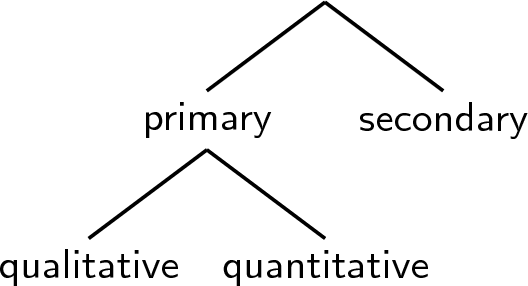
\includegraphics[width=300px]{col11306.imgs/m39403_MG10C16_001.png} % m39403;MG10C16\_001.png;;;6.0;8.5;
      \vspace{2pt}
    \vspace{\rubberspace}\par \begin{cnxcaption}
	  \small \textbf{Figure 16.1: }Classes of data.
	\end{cnxcaption}
    \vspace{.1in}
    \rule[.1in]{\figurerulewidth}{.005in} \\
    \end{center}
 \end{figure}       
          \label{m39403*id200390}\begin{description}[noitemsep]
            \label{m39403*uid4}
            \item[Primary data:]
          describes the original data that have been collected. This type of data is also known as \textsl{raw} data. Often the primary data set is very large and is therefore summarised or processed to extract meaningful information.
\label{m39403*uid5}
            \item[Qualitative data:]
          is information that cannot be written as numbers, for example, if you were collecting data from people on how they feel or what their favourite colour is.
\label{m39403*uid6}
            \item[Quantitative data:]
          is information that can be written as numbers, for example, if you were collecting data from people on their height or weight.
\label{m39403*uid7}
            \item[Secondary data:]
          is primary data that has been summarised or processed, for example, the set of colours that people gave as favourite colours would be secondary data because it is a summary of responses.
\end{itemize}
          \label{m39403*id200459}Transforming primary data into secondary data through analysis, grouping or organisation into secondary data is the process of generating information.\par 
        \label{m39403*uid8}
            \subsubsection{ Purpose of Collecting Primary Data}
            \nopagebreak
          \label{m39403*id200473}Data is collected to provide answers that help with understanding a particular situation. Here are examples to illustrate some real world data collections scenarios in the categories of qualitative and quantitative data.\par 
        \label{m39403*id200480}
            \subsubsection{ Qualitative Data}
            \nopagebreak
          \label{m39403*id200486}\begin{itemize}[noitemsep]
            \label{m39403*uid9}\item The local government might want to know how many residents have electricity and might ask the question: "Does your home have a safe, independent supply of electricity?"
\label{m39403*uid10}\item A supermarket manager might ask the question: ``What flavours of soft drink should be stocked in my supermarket?" The question asked of customers might be ``What is your favourite soft drink?'' Based on the customers' responses (i.e. which flavours are chosen), the manager can make an informed decision as to what soft drinks to stock.
\label{m39403*uid11}\item A company manufacturing medicines might ask ``How effective is our pill at relieving a headache?'' The question asked of people using the pill for a headache might be: ``Does taking the pill relieve your headache?'' Based on responses, the company learns how effective their product is.
\label{m39403*uid12}\item A motor car company might want to improve their customer service, and might ask their customers: ``How can we improve our customer service?''
\end{itemize}
        \label{m39403*id200551}
            \subsubsection{ Quantitative Data}
            \nopagebreak
          \label{m39403*id200557}\begin{itemize}[noitemsep]
            \label{m39403*uid13}\item A cell phone manufacturing company might collect data about how often people buy new cell phones and what factors affect their choice, so that the cell phone company can focus on those features that would make their product more attractive to buyers.
\label{m39403*uid14}\item A town councillor might want to know how many accidents have occurred at a particular intersection, to decide whether a robot should be installed. The councillor would visit the local police station to research their records to collect the appropriate data.
\label{m39403*uid15}\item A supermarket manager might ask the question: ``What flavours of soft drink should be stocked in my supermarket?" The question asked of customers might be ``What is your favourite soft drink?'' Based on the customers' responses (i.e. the number of customers who liked soft drink A), the manager can make an informed decision as to what soft drinks to stock. 
\end{itemize}
          \label{m39403*id200605}However, it is important to note that different questions reveal different features of a situation, and that this affects the ability to understand
the situation. For example, if the first question in the list was re-phrased to be: "Does your home have electricity?" then if you answered yes, but you were getting your electricity from a neighbour, then this would give the wrong impression that you did not need an independent supply of electricity.\par 
      \label{m39403*uid16}
            \subsubsection{ Methods of Data Collection}
            \nopagebreak
        \label{m39403*id200621}The method of collecting the data must be appropriate to the question being asked. Some examples of data collecting methods are:\par 
        \label{m39403*id200626}\begin{enumerate}[noitemsep, label=\textbf{\arabic*}. ] 
            \label{m39403*uid17}\item Questionnaires, surveys and interviews
\label{m39403*uid18}\item Experiments
\label{m39403*uid19}\item Other sources (friends, family, newspapers, books, magazines and the Internet)
\end{enumerate}
        \label{m39403*id200664}The most important aspect of each method of data collecting is to clearly formulate the question that is to be answered. The details of the data collection should therefore be structured to take your question into account.\par 
        \label{m39403*id200670}For example, questionnaires, interviews or surveys would be most appropriate for the list of questions in "Purpose of Collecting Primary Data" (Section~16.1.2.1.2: Purpose of Collecting Primary Data).\par 
      \label{m39403*uid20}
            \subsubsection{ Samples and Populations}
            \nopagebreak
        \label{m39403*id200688}Before the data collecting starts, it is important to decide how much data is needed to make sure that the results give an accurate reflection to the required answers. Ideally, the study should be designed to maximise the amount of information collected while minimising the effort. The concepts of \textsl{populations} and \textsl{samples} is vital to minimising effort.\par 
        \label{m39403*id200705}The following terms should be familiar:\par 
        \label{m39403*id200708}\begin{description}[noitemsep]
            \label{m39403*uid21}
            \item[Population:]
          describes the entire group under consideration in a study. For example, if you wanted to know how many learners in your school got the flu each winter, then your population would be all the learners in your school.
\label{m39403*uid22}
            \item[Sample:]
          describes a group chosen to represent the population under consideration in a study. For example, for the survey on winter flu, you might select a sample of learners, maybe one from each class.
\label{m39403*uid23}
            \item[Random sample:]
          describes a sample chosen from a population in such a way that each member of the population has an equal chance of being chosen.
\end{itemize}
        \label{m39403*id200757}
    \setcounter{subfigure}{0}
	\begin{figure}[H] % horizontal\label{m39403*id200760}
    \begin{center}
    \label{m39403*id200760!!!underscore!!!media}\label{m39403*id200760!!!underscore!!!printimage}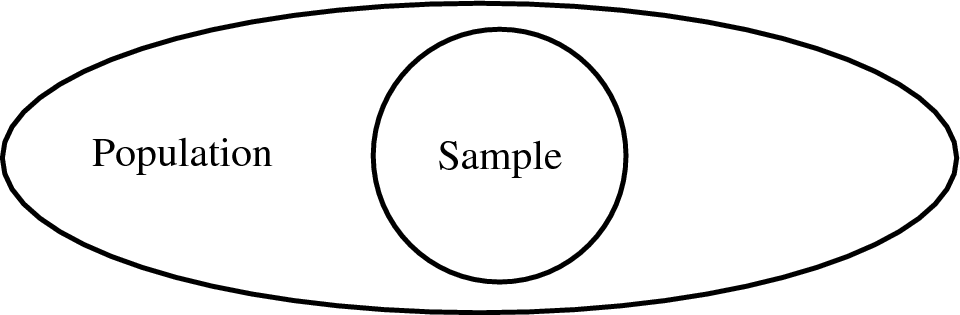
\includegraphics[width=300px]{col11306.imgs/m39403_MG10C16_002.png} % m39403;MG10C16\_002.png;;;6.0;8.5;
      \vspace{2pt}
    \vspace{.1in}
    \end{center}
 \end{figure}       
        \par 
        \label{m39403*id200766}Choosing a representative sample is crucial to obtaining results that are unbiased. For example, if we wanted to determine whether peer pressure affects the decision to start smoking, then the results would be different if only boys were interviewed, compared to if only girls were interviewed, compared to both boys and girls being interviewed.\par 
        \label{m39403*id200773}Therefore questions like: "How many interviews are needed?" and "How do I select the candidates for the interviews?" must be asked during the design stage of the sampling process.\par 
        \label{m39403*id200777}The most accurate results are obtained if the entire population is sampled for the survey, but this is expensive and time-consuming. The next best method is to \textsl{randomly} select a sample of subjects for the interviews. This means that whatever the method used to select subjects for the interviews, each subject has an equal chance of being selected. There are various methods of doing this for example, names can be picked out of a hat or can be selected by using a random number generator. Most modern scientific calculators have a random number generator or you can find one on a spreadsheet program on a computer.\par 
        \label{m39403*id200791}So, if you had a total population of 1 000 learners in your school and you randomly selected 100, then that would be the sample that is used to conduct your survey.\par 
    \label{m39403*cid4}
            \subsection{ Example Data Sets}
            \nopagebreak
      \label{m39403*id200805}The remainder of this chapter deals with the mathematical details that are required to analyse the data collected.\par 
      \label{m39403*id200809}The following are some example sets of data which can be used to apply the methods that are being explained.\par 
      \label{m39403*uid24}
            \subsubsection{ Data Set 1: Tossing a Coin}
            \nopagebreak
        \label{m39403*id200822}A fair coin was tossed 100 times and the values on the top face were recorded. The data are recorded in "Data Set 1: Tossing a coin" (Table 16.1).\par 
    % \textbf{m39403*uid25}\par
    % how many colspecs?  10
          % name: cnx:colspec
            % colnum: 1
            % colwidth: 10*
            % latex-name: columna
            % colname: 
            % align/tgroup-align/default: //left
            % -------------------------
            % name: cnx:colspec
            % colnum: 2
            % colwidth: 10*
            % latex-name: columnb
            % colname: 
            % align/tgroup-align/default: //left
            % -------------------------
            % name: cnx:colspec
            % colnum: 3
            % colwidth: 10*
            % latex-name: columnc
            % colname: 
            % align/tgroup-align/default: //left
            % -------------------------
            % name: cnx:colspec
            % colnum: 4
            % colwidth: 10*
            % latex-name: columnd
            % colname: 
            % align/tgroup-align/default: //left
            % -------------------------
            % name: cnx:colspec
            % colnum: 5
            % colwidth: 10*
            % latex-name: columne
            % colname: 
            % align/tgroup-align/default: //left
            % -------------------------
            % name: cnx:colspec
            % colnum: 6
            % colwidth: 10*
            % latex-name: columnf
            % colname: 
            % align/tgroup-align/default: //left
            % -------------------------
            % name: cnx:colspec
            % colnum: 7
            % colwidth: 10*
            % latex-name: columng
            % colname: 
            % align/tgroup-align/default: //left
            % -------------------------
            % name: cnx:colspec
            % colnum: 8
            % colwidth: 10*
            % latex-name: columnh
            % colname: 
            % align/tgroup-align/default: //left
            % -------------------------
            % name: cnx:colspec
            % colnum: 9
            % colwidth: 10*
            % latex-name: columni
            % colname: 
            % align/tgroup-align/default: //left
            % -------------------------
            % name: cnx:colspec
            % colnum: 10
            % colwidth: 10*
            % latex-name: columnj
            % colname: 
            % align/tgroup-align/default: //left
            % -------------------------
    \setlength\mytablespace{20\tabcolsep}
    \addtolength\mytablespace{11\arrayrulewidth}
    \setlength\mytablewidth{\linewidth}
    \setlength\mytableroom{\mytablewidth}
    \addtolength\mytableroom{-\mytablespace}
    \setlength\myfixedwidth{0pt}
    \setlength\mystarwidth{\mytableroom}
        \addtolength\mystarwidth{-\myfixedwidth}
        \divide\mystarwidth 100
      % ----- Begin capturing width of table in LR mode woof
      \settowidth{\mytableboxwidth}{\begin{tabular}[t]{|l|l|l|l|l|l|l|l|l|l|}\hline
    % count in rowspan-info-nodeset: 10
    % align/colidx: left,1
    % rowcount: '0' | start: 'false' | colidx: '1'
        % Formatting a regular cell and recurring on the next sibling
        H &
      % align/colidx: left,2
    % rowcount: '0' | start: 'false' | colidx: '2'
        % Formatting a regular cell and recurring on the next sibling
        T &
      % align/colidx: left,3
    % rowcount: '0' | start: 'false' | colidx: '3'
        % Formatting a regular cell and recurring on the next sibling
        T &
      % align/colidx: left,4
    % rowcount: '0' | start: 'false' | colidx: '4'
        % Formatting a regular cell and recurring on the next sibling
        H &
      % align/colidx: left,5
    % rowcount: '0' | start: 'false' | colidx: '5'
        % Formatting a regular cell and recurring on the next sibling
        H &
      % align/colidx: left,6
    % rowcount: '0' | start: 'false' | colidx: '6'
        % Formatting a regular cell and recurring on the next sibling
        T &
      % align/colidx: left,7
    % rowcount: '0' | start: 'false' | colidx: '7'
        % Formatting a regular cell and recurring on the next sibling
        H &
      % align/colidx: left,8
    % rowcount: '0' | start: 'false' | colidx: '8'
        % Formatting a regular cell and recurring on the next sibling
        H &
      % align/colidx: left,9
    % rowcount: '0' | start: 'false' | colidx: '9'
        % Formatting a regular cell and recurring on the next sibling
        H &
      % align/colidx: left,10
    % rowcount: '0' | start: 'false' | colidx: '10'
        % Formatting a regular cell and recurring on the next sibling
        H% make-rowspan-placeholders
    % rowspan info: col1 '0' | 'false' | '' || col2 '0' | 'false' | '' || col3 '0' | 'false' | '' || col4 '0' | 'false' | '' || col5 '0' | 'false' | '' || col6 '0' | 'false' | '' || col7 '0' | 'false' | '' || col8 '0' | 'false' | '' || col9 '0' | 'false' | '' || col10 '0' | 'false' | ''
     \tabularnewline\cline{1-1}\cline{2-2}\cline{3-3}\cline{4-4}\cline{5-5}\cline{6-6}\cline{7-7}\cline{8-8}\cline{9-9}\cline{10-10}
      %--------------------------------------------------------------------
    % align/colidx: left,1
    % rowcount: '0' | start: 'false' | colidx: '1'
        % Formatting a regular cell and recurring on the next sibling
        H &
      % align/colidx: left,2
    % rowcount: '0' | start: 'false' | colidx: '2'
        % Formatting a regular cell and recurring on the next sibling
        H &
      % align/colidx: left,3
    % rowcount: '0' | start: 'false' | colidx: '3'
        % Formatting a regular cell and recurring on the next sibling
        H &
      % align/colidx: left,4
    % rowcount: '0' | start: 'false' | colidx: '4'
        % Formatting a regular cell and recurring on the next sibling
        H &
      % align/colidx: left,5
    % rowcount: '0' | start: 'false' | colidx: '5'
        % Formatting a regular cell and recurring on the next sibling
        T &
      % align/colidx: left,6
    % rowcount: '0' | start: 'false' | colidx: '6'
        % Formatting a regular cell and recurring on the next sibling
        H &
      % align/colidx: left,7
    % rowcount: '0' | start: 'false' | colidx: '7'
        % Formatting a regular cell and recurring on the next sibling
        H &
      % align/colidx: left,8
    % rowcount: '0' | start: 'false' | colidx: '8'
        % Formatting a regular cell and recurring on the next sibling
        T &
      % align/colidx: left,9
    % rowcount: '0' | start: 'false' | colidx: '9'
        % Formatting a regular cell and recurring on the next sibling
        T &
      % align/colidx: left,10
    % rowcount: '0' | start: 'false' | colidx: '10'
        % Formatting a regular cell and recurring on the next sibling
        T% make-rowspan-placeholders
    % rowspan info: col1 '0' | 'false' | '' || col2 '0' | 'false' | '' || col3 '0' | 'false' | '' || col4 '0' | 'false' | '' || col5 '0' | 'false' | '' || col6 '0' | 'false' | '' || col7 '0' | 'false' | '' || col8 '0' | 'false' | '' || col9 '0' | 'false' | '' || col10 '0' | 'false' | ''
     \tabularnewline\cline{1-1}\cline{2-2}\cline{3-3}\cline{4-4}\cline{5-5}\cline{6-6}\cline{7-7}\cline{8-8}\cline{9-9}\cline{10-10}
      %--------------------------------------------------------------------
    % align/colidx: left,1
    % rowcount: '0' | start: 'false' | colidx: '1'
        % Formatting a regular cell and recurring on the next sibling
        T &
      % align/colidx: left,2
    % rowcount: '0' | start: 'false' | colidx: '2'
        % Formatting a regular cell and recurring on the next sibling
        T &
      % align/colidx: left,3
    % rowcount: '0' | start: 'false' | colidx: '3'
        % Formatting a regular cell and recurring on the next sibling
        H &
      % align/colidx: left,4
    % rowcount: '0' | start: 'false' | colidx: '4'
        % Formatting a regular cell and recurring on the next sibling
        T &
      % align/colidx: left,5
    % rowcount: '0' | start: 'false' | colidx: '5'
        % Formatting a regular cell and recurring on the next sibling
        T &
      % align/colidx: left,6
    % rowcount: '0' | start: 'false' | colidx: '6'
        % Formatting a regular cell and recurring on the next sibling
        H &
      % align/colidx: left,7
    % rowcount: '0' | start: 'false' | colidx: '7'
        % Formatting a regular cell and recurring on the next sibling
        T &
      % align/colidx: left,8
    % rowcount: '0' | start: 'false' | colidx: '8'
        % Formatting a regular cell and recurring on the next sibling
        H &
      % align/colidx: left,9
    % rowcount: '0' | start: 'false' | colidx: '9'
        % Formatting a regular cell and recurring on the next sibling
        T &
      % align/colidx: left,10
    % rowcount: '0' | start: 'false' | colidx: '10'
        % Formatting a regular cell and recurring on the next sibling
        H% make-rowspan-placeholders
    % rowspan info: col1 '0' | 'false' | '' || col2 '0' | 'false' | '' || col3 '0' | 'false' | '' || col4 '0' | 'false' | '' || col5 '0' | 'false' | '' || col6 '0' | 'false' | '' || col7 '0' | 'false' | '' || col8 '0' | 'false' | '' || col9 '0' | 'false' | '' || col10 '0' | 'false' | ''
     \tabularnewline\cline{1-1}\cline{2-2}\cline{3-3}\cline{4-4}\cline{5-5}\cline{6-6}\cline{7-7}\cline{8-8}\cline{9-9}\cline{10-10}
      %--------------------------------------------------------------------
    % align/colidx: left,1
    % rowcount: '0' | start: 'false' | colidx: '1'
        % Formatting a regular cell and recurring on the next sibling
        H &
      % align/colidx: left,2
    % rowcount: '0' | start: 'false' | colidx: '2'
        % Formatting a regular cell and recurring on the next sibling
        H &
      % align/colidx: left,3
    % rowcount: '0' | start: 'false' | colidx: '3'
        % Formatting a regular cell and recurring on the next sibling
        T &
      % align/colidx: left,4
    % rowcount: '0' | start: 'false' | colidx: '4'
        % Formatting a regular cell and recurring on the next sibling
        T &
      % align/colidx: left,5
    % rowcount: '0' | start: 'false' | colidx: '5'
        % Formatting a regular cell and recurring on the next sibling
        H &
      % align/colidx: left,6
    % rowcount: '0' | start: 'false' | colidx: '6'
        % Formatting a regular cell and recurring on the next sibling
        T &
      % align/colidx: left,7
    % rowcount: '0' | start: 'false' | colidx: '7'
        % Formatting a regular cell and recurring on the next sibling
        T &
      % align/colidx: left,8
    % rowcount: '0' | start: 'false' | colidx: '8'
        % Formatting a regular cell and recurring on the next sibling
        H &
      % align/colidx: left,9
    % rowcount: '0' | start: 'false' | colidx: '9'
        % Formatting a regular cell and recurring on the next sibling
        T &
      % align/colidx: left,10
    % rowcount: '0' | start: 'false' | colidx: '10'
        % Formatting a regular cell and recurring on the next sibling
        T% make-rowspan-placeholders
    % rowspan info: col1 '0' | 'false' | '' || col2 '0' | 'false' | '' || col3 '0' | 'false' | '' || col4 '0' | 'false' | '' || col5 '0' | 'false' | '' || col6 '0' | 'false' | '' || col7 '0' | 'false' | '' || col8 '0' | 'false' | '' || col9 '0' | 'false' | '' || col10 '0' | 'false' | ''
     \tabularnewline\cline{1-1}\cline{2-2}\cline{3-3}\cline{4-4}\cline{5-5}\cline{6-6}\cline{7-7}\cline{8-8}\cline{9-9}\cline{10-10}
      %--------------------------------------------------------------------
    % align/colidx: left,1
    % rowcount: '0' | start: 'false' | colidx: '1'
        % Formatting a regular cell and recurring on the next sibling
        T &
      % align/colidx: left,2
    % rowcount: '0' | start: 'false' | colidx: '2'
        % Formatting a regular cell and recurring on the next sibling
        H &
      % align/colidx: left,3
    % rowcount: '0' | start: 'false' | colidx: '3'
        % Formatting a regular cell and recurring on the next sibling
        H &
      % align/colidx: left,4
    % rowcount: '0' | start: 'false' | colidx: '4'
        % Formatting a regular cell and recurring on the next sibling
        H &
      % align/colidx: left,5
    % rowcount: '0' | start: 'false' | colidx: '5'
        % Formatting a regular cell and recurring on the next sibling
        T &
      % align/colidx: left,6
    % rowcount: '0' | start: 'false' | colidx: '6'
        % Formatting a regular cell and recurring on the next sibling
        T &
      % align/colidx: left,7
    % rowcount: '0' | start: 'false' | colidx: '7'
        % Formatting a regular cell and recurring on the next sibling
        H &
      % align/colidx: left,8
    % rowcount: '0' | start: 'false' | colidx: '8'
        % Formatting a regular cell and recurring on the next sibling
        T &
      % align/colidx: left,9
    % rowcount: '0' | start: 'false' | colidx: '9'
        % Formatting a regular cell and recurring on the next sibling
        T &
      % align/colidx: left,10
    % rowcount: '0' | start: 'false' | colidx: '10'
        % Formatting a regular cell and recurring on the next sibling
        H% make-rowspan-placeholders
    % rowspan info: col1 '0' | 'false' | '' || col2 '0' | 'false' | '' || col3 '0' | 'false' | '' || col4 '0' | 'false' | '' || col5 '0' | 'false' | '' || col6 '0' | 'false' | '' || col7 '0' | 'false' | '' || col8 '0' | 'false' | '' || col9 '0' | 'false' | '' || col10 '0' | 'false' | ''
     \tabularnewline\cline{1-1}\cline{2-2}\cline{3-3}\cline{4-4}\cline{5-5}\cline{6-6}\cline{7-7}\cline{8-8}\cline{9-9}\cline{10-10}
      %--------------------------------------------------------------------
    % align/colidx: left,1
    % rowcount: '0' | start: 'false' | colidx: '1'
        % Formatting a regular cell and recurring on the next sibling
        H &
      % align/colidx: left,2
    % rowcount: '0' | start: 'false' | colidx: '2'
        % Formatting a regular cell and recurring on the next sibling
        T &
      % align/colidx: left,3
    % rowcount: '0' | start: 'false' | colidx: '3'
        % Formatting a regular cell and recurring on the next sibling
        T &
      % align/colidx: left,4
    % rowcount: '0' | start: 'false' | colidx: '4'
        % Formatting a regular cell and recurring on the next sibling
        T &
      % align/colidx: left,5
    % rowcount: '0' | start: 'false' | colidx: '5'
        % Formatting a regular cell and recurring on the next sibling
        T &
      % align/colidx: left,6
    % rowcount: '0' | start: 'false' | colidx: '6'
        % Formatting a regular cell and recurring on the next sibling
        H &
      % align/colidx: left,7
    % rowcount: '0' | start: 'false' | colidx: '7'
        % Formatting a regular cell and recurring on the next sibling
        T &
      % align/colidx: left,8
    % rowcount: '0' | start: 'false' | colidx: '8'
        % Formatting a regular cell and recurring on the next sibling
        T &
      % align/colidx: left,9
    % rowcount: '0' | start: 'false' | colidx: '9'
        % Formatting a regular cell and recurring on the next sibling
        H &
      % align/colidx: left,10
    % rowcount: '0' | start: 'false' | colidx: '10'
        % Formatting a regular cell and recurring on the next sibling
        H% make-rowspan-placeholders
    % rowspan info: col1 '0' | 'false' | '' || col2 '0' | 'false' | '' || col3 '0' | 'false' | '' || col4 '0' | 'false' | '' || col5 '0' | 'false' | '' || col6 '0' | 'false' | '' || col7 '0' | 'false' | '' || col8 '0' | 'false' | '' || col9 '0' | 'false' | '' || col10 '0' | 'false' | ''
     \tabularnewline\cline{1-1}\cline{2-2}\cline{3-3}\cline{4-4}\cline{5-5}\cline{6-6}\cline{7-7}\cline{8-8}\cline{9-9}\cline{10-10}
      %--------------------------------------------------------------------
    % align/colidx: left,1
    % rowcount: '0' | start: 'false' | colidx: '1'
        % Formatting a regular cell and recurring on the next sibling
        T &
      % align/colidx: left,2
    % rowcount: '0' | start: 'false' | colidx: '2'
        % Formatting a regular cell and recurring on the next sibling
        T &
      % align/colidx: left,3
    % rowcount: '0' | start: 'false' | colidx: '3'
        % Formatting a regular cell and recurring on the next sibling
        H &
      % align/colidx: left,4
    % rowcount: '0' | start: 'false' | colidx: '4'
        % Formatting a regular cell and recurring on the next sibling
        T &
      % align/colidx: left,5
    % rowcount: '0' | start: 'false' | colidx: '5'
        % Formatting a regular cell and recurring on the next sibling
        T &
      % align/colidx: left,6
    % rowcount: '0' | start: 'false' | colidx: '6'
        % Formatting a regular cell and recurring on the next sibling
        H &
      % align/colidx: left,7
    % rowcount: '0' | start: 'false' | colidx: '7'
        % Formatting a regular cell and recurring on the next sibling
        T &
      % align/colidx: left,8
    % rowcount: '0' | start: 'false' | colidx: '8'
        % Formatting a regular cell and recurring on the next sibling
        T &
      % align/colidx: left,9
    % rowcount: '0' | start: 'false' | colidx: '9'
        % Formatting a regular cell and recurring on the next sibling
        H &
      % align/colidx: left,10
    % rowcount: '0' | start: 'false' | colidx: '10'
        % Formatting a regular cell and recurring on the next sibling
        T% make-rowspan-placeholders
    % rowspan info: col1 '0' | 'false' | '' || col2 '0' | 'false' | '' || col3 '0' | 'false' | '' || col4 '0' | 'false' | '' || col5 '0' | 'false' | '' || col6 '0' | 'false' | '' || col7 '0' | 'false' | '' || col8 '0' | 'false' | '' || col9 '0' | 'false' | '' || col10 '0' | 'false' | ''
     \tabularnewline\cline{1-1}\cline{2-2}\cline{3-3}\cline{4-4}\cline{5-5}\cline{6-6}\cline{7-7}\cline{8-8}\cline{9-9}\cline{10-10}
      %--------------------------------------------------------------------
    % align/colidx: left,1
    % rowcount: '0' | start: 'false' | colidx: '1'
        % Formatting a regular cell and recurring on the next sibling
        H &
      % align/colidx: left,2
    % rowcount: '0' | start: 'false' | colidx: '2'
        % Formatting a regular cell and recurring on the next sibling
        T &
      % align/colidx: left,3
    % rowcount: '0' | start: 'false' | colidx: '3'
        % Formatting a regular cell and recurring on the next sibling
        T &
      % align/colidx: left,4
    % rowcount: '0' | start: 'false' | colidx: '4'
        % Formatting a regular cell and recurring on the next sibling
        H &
      % align/colidx: left,5
    % rowcount: '0' | start: 'false' | colidx: '5'
        % Formatting a regular cell and recurring on the next sibling
        T &
      % align/colidx: left,6
    % rowcount: '0' | start: 'false' | colidx: '6'
        % Formatting a regular cell and recurring on the next sibling
        T &
      % align/colidx: left,7
    % rowcount: '0' | start: 'false' | colidx: '7'
        % Formatting a regular cell and recurring on the next sibling
        T &
      % align/colidx: left,8
    % rowcount: '0' | start: 'false' | colidx: '8'
        % Formatting a regular cell and recurring on the next sibling
        T &
      % align/colidx: left,9
    % rowcount: '0' | start: 'false' | colidx: '9'
        % Formatting a regular cell and recurring on the next sibling
        H &
      % align/colidx: left,10
    % rowcount: '0' | start: 'false' | colidx: '10'
        % Formatting a regular cell and recurring on the next sibling
        T% make-rowspan-placeholders
    % rowspan info: col1 '0' | 'false' | '' || col2 '0' | 'false' | '' || col3 '0' | 'false' | '' || col4 '0' | 'false' | '' || col5 '0' | 'false' | '' || col6 '0' | 'false' | '' || col7 '0' | 'false' | '' || col8 '0' | 'false' | '' || col9 '0' | 'false' | '' || col10 '0' | 'false' | ''
     \tabularnewline\cline{1-1}\cline{2-2}\cline{3-3}\cline{4-4}\cline{5-5}\cline{6-6}\cline{7-7}\cline{8-8}\cline{9-9}\cline{10-10}
      %--------------------------------------------------------------------
    % align/colidx: left,1
    % rowcount: '0' | start: 'false' | colidx: '1'
        % Formatting a regular cell and recurring on the next sibling
        T &
      % align/colidx: left,2
    % rowcount: '0' | start: 'false' | colidx: '2'
        % Formatting a regular cell and recurring on the next sibling
        H &
      % align/colidx: left,3
    % rowcount: '0' | start: 'false' | colidx: '3'
        % Formatting a regular cell and recurring on the next sibling
        T &
      % align/colidx: left,4
    % rowcount: '0' | start: 'false' | colidx: '4'
        % Formatting a regular cell and recurring on the next sibling
        T &
      % align/colidx: left,5
    % rowcount: '0' | start: 'false' | colidx: '5'
        % Formatting a regular cell and recurring on the next sibling
        H &
      % align/colidx: left,6
    % rowcount: '0' | start: 'false' | colidx: '6'
        % Formatting a regular cell and recurring on the next sibling
        H &
      % align/colidx: left,7
    % rowcount: '0' | start: 'false' | colidx: '7'
        % Formatting a regular cell and recurring on the next sibling
        H &
      % align/colidx: left,8
    % rowcount: '0' | start: 'false' | colidx: '8'
        % Formatting a regular cell and recurring on the next sibling
        T &
      % align/colidx: left,9
    % rowcount: '0' | start: 'false' | colidx: '9'
        % Formatting a regular cell and recurring on the next sibling
        H &
      % align/colidx: left,10
    % rowcount: '0' | start: 'false' | colidx: '10'
        % Formatting a regular cell and recurring on the next sibling
        T% make-rowspan-placeholders
    % rowspan info: col1 '0' | 'false' | '' || col2 '0' | 'false' | '' || col3 '0' | 'false' | '' || col4 '0' | 'false' | '' || col5 '0' | 'false' | '' || col6 '0' | 'false' | '' || col7 '0' | 'false' | '' || col8 '0' | 'false' | '' || col9 '0' | 'false' | '' || col10 '0' | 'false' | ''
     \tabularnewline\cline{1-1}\cline{2-2}\cline{3-3}\cline{4-4}\cline{5-5}\cline{6-6}\cline{7-7}\cline{8-8}\cline{9-9}\cline{10-10}
      %--------------------------------------------------------------------
    % align/colidx: left,1
    % rowcount: '0' | start: 'false' | colidx: '1'
        % Formatting a regular cell and recurring on the next sibling
        T &
      % align/colidx: left,2
    % rowcount: '0' | start: 'false' | colidx: '2'
        % Formatting a regular cell and recurring on the next sibling
        T &
      % align/colidx: left,3
    % rowcount: '0' | start: 'false' | colidx: '3'
        % Formatting a regular cell and recurring on the next sibling
        T &
      % align/colidx: left,4
    % rowcount: '0' | start: 'false' | colidx: '4'
        % Formatting a regular cell and recurring on the next sibling
        H &
      % align/colidx: left,5
    % rowcount: '0' | start: 'false' | colidx: '5'
        % Formatting a regular cell and recurring on the next sibling
        H &
      % align/colidx: left,6
    % rowcount: '0' | start: 'false' | colidx: '6'
        % Formatting a regular cell and recurring on the next sibling
        T &
      % align/colidx: left,7
    % rowcount: '0' | start: 'false' | colidx: '7'
        % Formatting a regular cell and recurring on the next sibling
        T &
      % align/colidx: left,8
    % rowcount: '0' | start: 'false' | colidx: '8'
        % Formatting a regular cell and recurring on the next sibling
        T &
      % align/colidx: left,9
    % rowcount: '0' | start: 'false' | colidx: '9'
        % Formatting a regular cell and recurring on the next sibling
        H &
      % align/colidx: left,10
    % rowcount: '0' | start: 'false' | colidx: '10'
        % Formatting a regular cell and recurring on the next sibling
        T% make-rowspan-placeholders
    % rowspan info: col1 '0' | 'false' | '' || col2 '0' | 'false' | '' || col3 '0' | 'false' | '' || col4 '0' | 'false' | '' || col5 '0' | 'false' | '' || col6 '0' | 'false' | '' || col7 '0' | 'false' | '' || col8 '0' | 'false' | '' || col9 '0' | 'false' | '' || col10 '0' | 'false' | ''
     \tabularnewline\cline{1-1}\cline{2-2}\cline{3-3}\cline{4-4}\cline{5-5}\cline{6-6}\cline{7-7}\cline{8-8}\cline{9-9}\cline{10-10}
      %--------------------------------------------------------------------
    \end{tabular}} % end mytableboxwidth set      
      % ----- End capturing width of table in LR mode
        % ----- LR or paragraph mode: must test
        % ----- Begin capturing height of table
        \settoheight{\mytableboxheight}{\begin{tabular}[t]{|l|l|l|l|l|l|l|l|l|l|}\hline
    % count in rowspan-info-nodeset: 10
    % align/colidx: left,1
    % rowcount: '0' | start: 'false' | colidx: '1'
        % Formatting a regular cell and recurring on the next sibling
        H &
      % align/colidx: left,2
    % rowcount: '0' | start: 'false' | colidx: '2'
        % Formatting a regular cell and recurring on the next sibling
        T &
      % align/colidx: left,3
    % rowcount: '0' | start: 'false' | colidx: '3'
        % Formatting a regular cell and recurring on the next sibling
        T &
      % align/colidx: left,4
    % rowcount: '0' | start: 'false' | colidx: '4'
        % Formatting a regular cell and recurring on the next sibling
        H &
      % align/colidx: left,5
    % rowcount: '0' | start: 'false' | colidx: '5'
        % Formatting a regular cell and recurring on the next sibling
        H &
      % align/colidx: left,6
    % rowcount: '0' | start: 'false' | colidx: '6'
        % Formatting a regular cell and recurring on the next sibling
        T &
      % align/colidx: left,7
    % rowcount: '0' | start: 'false' | colidx: '7'
        % Formatting a regular cell and recurring on the next sibling
        H &
      % align/colidx: left,8
    % rowcount: '0' | start: 'false' | colidx: '8'
        % Formatting a regular cell and recurring on the next sibling
        H &
      % align/colidx: left,9
    % rowcount: '0' | start: 'false' | colidx: '9'
        % Formatting a regular cell and recurring on the next sibling
        H &
      % align/colidx: left,10
    % rowcount: '0' | start: 'false' | colidx: '10'
        % Formatting a regular cell and recurring on the next sibling
        H% make-rowspan-placeholders
    % rowspan info: col1 '0' | 'false' | '' || col2 '0' | 'false' | '' || col3 '0' | 'false' | '' || col4 '0' | 'false' | '' || col5 '0' | 'false' | '' || col6 '0' | 'false' | '' || col7 '0' | 'false' | '' || col8 '0' | 'false' | '' || col9 '0' | 'false' | '' || col10 '0' | 'false' | ''
     \tabularnewline\cline{1-1}\cline{2-2}\cline{3-3}\cline{4-4}\cline{5-5}\cline{6-6}\cline{7-7}\cline{8-8}\cline{9-9}\cline{10-10}
      %--------------------------------------------------------------------
    % align/colidx: left,1
    % rowcount: '0' | start: 'false' | colidx: '1'
        % Formatting a regular cell and recurring on the next sibling
        H &
      % align/colidx: left,2
    % rowcount: '0' | start: 'false' | colidx: '2'
        % Formatting a regular cell and recurring on the next sibling
        H &
      % align/colidx: left,3
    % rowcount: '0' | start: 'false' | colidx: '3'
        % Formatting a regular cell and recurring on the next sibling
        H &
      % align/colidx: left,4
    % rowcount: '0' | start: 'false' | colidx: '4'
        % Formatting a regular cell and recurring on the next sibling
        H &
      % align/colidx: left,5
    % rowcount: '0' | start: 'false' | colidx: '5'
        % Formatting a regular cell and recurring on the next sibling
        T &
      % align/colidx: left,6
    % rowcount: '0' | start: 'false' | colidx: '6'
        % Formatting a regular cell and recurring on the next sibling
        H &
      % align/colidx: left,7
    % rowcount: '0' | start: 'false' | colidx: '7'
        % Formatting a regular cell and recurring on the next sibling
        H &
      % align/colidx: left,8
    % rowcount: '0' | start: 'false' | colidx: '8'
        % Formatting a regular cell and recurring on the next sibling
        T &
      % align/colidx: left,9
    % rowcount: '0' | start: 'false' | colidx: '9'
        % Formatting a regular cell and recurring on the next sibling
        T &
      % align/colidx: left,10
    % rowcount: '0' | start: 'false' | colidx: '10'
        % Formatting a regular cell and recurring on the next sibling
        T% make-rowspan-placeholders
    % rowspan info: col1 '0' | 'false' | '' || col2 '0' | 'false' | '' || col3 '0' | 'false' | '' || col4 '0' | 'false' | '' || col5 '0' | 'false' | '' || col6 '0' | 'false' | '' || col7 '0' | 'false' | '' || col8 '0' | 'false' | '' || col9 '0' | 'false' | '' || col10 '0' | 'false' | ''
     \tabularnewline\cline{1-1}\cline{2-2}\cline{3-3}\cline{4-4}\cline{5-5}\cline{6-6}\cline{7-7}\cline{8-8}\cline{9-9}\cline{10-10}
      %--------------------------------------------------------------------
    % align/colidx: left,1
    % rowcount: '0' | start: 'false' | colidx: '1'
        % Formatting a regular cell and recurring on the next sibling
        T &
      % align/colidx: left,2
    % rowcount: '0' | start: 'false' | colidx: '2'
        % Formatting a regular cell and recurring on the next sibling
        T &
      % align/colidx: left,3
    % rowcount: '0' | start: 'false' | colidx: '3'
        % Formatting a regular cell and recurring on the next sibling
        H &
      % align/colidx: left,4
    % rowcount: '0' | start: 'false' | colidx: '4'
        % Formatting a regular cell and recurring on the next sibling
        T &
      % align/colidx: left,5
    % rowcount: '0' | start: 'false' | colidx: '5'
        % Formatting a regular cell and recurring on the next sibling
        T &
      % align/colidx: left,6
    % rowcount: '0' | start: 'false' | colidx: '6'
        % Formatting a regular cell and recurring on the next sibling
        H &
      % align/colidx: left,7
    % rowcount: '0' | start: 'false' | colidx: '7'
        % Formatting a regular cell and recurring on the next sibling
        T &
      % align/colidx: left,8
    % rowcount: '0' | start: 'false' | colidx: '8'
        % Formatting a regular cell and recurring on the next sibling
        H &
      % align/colidx: left,9
    % rowcount: '0' | start: 'false' | colidx: '9'
        % Formatting a regular cell and recurring on the next sibling
        T &
      % align/colidx: left,10
    % rowcount: '0' | start: 'false' | colidx: '10'
        % Formatting a regular cell and recurring on the next sibling
        H% make-rowspan-placeholders
    % rowspan info: col1 '0' | 'false' | '' || col2 '0' | 'false' | '' || col3 '0' | 'false' | '' || col4 '0' | 'false' | '' || col5 '0' | 'false' | '' || col6 '0' | 'false' | '' || col7 '0' | 'false' | '' || col8 '0' | 'false' | '' || col9 '0' | 'false' | '' || col10 '0' | 'false' | ''
     \tabularnewline\cline{1-1}\cline{2-2}\cline{3-3}\cline{4-4}\cline{5-5}\cline{6-6}\cline{7-7}\cline{8-8}\cline{9-9}\cline{10-10}
      %--------------------------------------------------------------------
    % align/colidx: left,1
    % rowcount: '0' | start: 'false' | colidx: '1'
        % Formatting a regular cell and recurring on the next sibling
        H &
      % align/colidx: left,2
    % rowcount: '0' | start: 'false' | colidx: '2'
        % Formatting a regular cell and recurring on the next sibling
        H &
      % align/colidx: left,3
    % rowcount: '0' | start: 'false' | colidx: '3'
        % Formatting a regular cell and recurring on the next sibling
        T &
      % align/colidx: left,4
    % rowcount: '0' | start: 'false' | colidx: '4'
        % Formatting a regular cell and recurring on the next sibling
        T &
      % align/colidx: left,5
    % rowcount: '0' | start: 'false' | colidx: '5'
        % Formatting a regular cell and recurring on the next sibling
        H &
      % align/colidx: left,6
    % rowcount: '0' | start: 'false' | colidx: '6'
        % Formatting a regular cell and recurring on the next sibling
        T &
      % align/colidx: left,7
    % rowcount: '0' | start: 'false' | colidx: '7'
        % Formatting a regular cell and recurring on the next sibling
        T &
      % align/colidx: left,8
    % rowcount: '0' | start: 'false' | colidx: '8'
        % Formatting a regular cell and recurring on the next sibling
        H &
      % align/colidx: left,9
    % rowcount: '0' | start: 'false' | colidx: '9'
        % Formatting a regular cell and recurring on the next sibling
        T &
      % align/colidx: left,10
    % rowcount: '0' | start: 'false' | colidx: '10'
        % Formatting a regular cell and recurring on the next sibling
        T% make-rowspan-placeholders
    % rowspan info: col1 '0' | 'false' | '' || col2 '0' | 'false' | '' || col3 '0' | 'false' | '' || col4 '0' | 'false' | '' || col5 '0' | 'false' | '' || col6 '0' | 'false' | '' || col7 '0' | 'false' | '' || col8 '0' | 'false' | '' || col9 '0' | 'false' | '' || col10 '0' | 'false' | ''
     \tabularnewline\cline{1-1}\cline{2-2}\cline{3-3}\cline{4-4}\cline{5-5}\cline{6-6}\cline{7-7}\cline{8-8}\cline{9-9}\cline{10-10}
      %--------------------------------------------------------------------
    % align/colidx: left,1
    % rowcount: '0' | start: 'false' | colidx: '1'
        % Formatting a regular cell and recurring on the next sibling
        T &
      % align/colidx: left,2
    % rowcount: '0' | start: 'false' | colidx: '2'
        % Formatting a regular cell and recurring on the next sibling
        H &
      % align/colidx: left,3
    % rowcount: '0' | start: 'false' | colidx: '3'
        % Formatting a regular cell and recurring on the next sibling
        H &
      % align/colidx: left,4
    % rowcount: '0' | start: 'false' | colidx: '4'
        % Formatting a regular cell and recurring on the next sibling
        H &
      % align/colidx: left,5
    % rowcount: '0' | start: 'false' | colidx: '5'
        % Formatting a regular cell and recurring on the next sibling
        T &
      % align/colidx: left,6
    % rowcount: '0' | start: 'false' | colidx: '6'
        % Formatting a regular cell and recurring on the next sibling
        T &
      % align/colidx: left,7
    % rowcount: '0' | start: 'false' | colidx: '7'
        % Formatting a regular cell and recurring on the next sibling
        H &
      % align/colidx: left,8
    % rowcount: '0' | start: 'false' | colidx: '8'
        % Formatting a regular cell and recurring on the next sibling
        T &
      % align/colidx: left,9
    % rowcount: '0' | start: 'false' | colidx: '9'
        % Formatting a regular cell and recurring on the next sibling
        T &
      % align/colidx: left,10
    % rowcount: '0' | start: 'false' | colidx: '10'
        % Formatting a regular cell and recurring on the next sibling
        H% make-rowspan-placeholders
    % rowspan info: col1 '0' | 'false' | '' || col2 '0' | 'false' | '' || col3 '0' | 'false' | '' || col4 '0' | 'false' | '' || col5 '0' | 'false' | '' || col6 '0' | 'false' | '' || col7 '0' | 'false' | '' || col8 '0' | 'false' | '' || col9 '0' | 'false' | '' || col10 '0' | 'false' | ''
     \tabularnewline\cline{1-1}\cline{2-2}\cline{3-3}\cline{4-4}\cline{5-5}\cline{6-6}\cline{7-7}\cline{8-8}\cline{9-9}\cline{10-10}
      %--------------------------------------------------------------------
    % align/colidx: left,1
    % rowcount: '0' | start: 'false' | colidx: '1'
        % Formatting a regular cell and recurring on the next sibling
        H &
      % align/colidx: left,2
    % rowcount: '0' | start: 'false' | colidx: '2'
        % Formatting a regular cell and recurring on the next sibling
        T &
      % align/colidx: left,3
    % rowcount: '0' | start: 'false' | colidx: '3'
        % Formatting a regular cell and recurring on the next sibling
        T &
      % align/colidx: left,4
    % rowcount: '0' | start: 'false' | colidx: '4'
        % Formatting a regular cell and recurring on the next sibling
        T &
      % align/colidx: left,5
    % rowcount: '0' | start: 'false' | colidx: '5'
        % Formatting a regular cell and recurring on the next sibling
        T &
      % align/colidx: left,6
    % rowcount: '0' | start: 'false' | colidx: '6'
        % Formatting a regular cell and recurring on the next sibling
        H &
      % align/colidx: left,7
    % rowcount: '0' | start: 'false' | colidx: '7'
        % Formatting a regular cell and recurring on the next sibling
        T &
      % align/colidx: left,8
    % rowcount: '0' | start: 'false' | colidx: '8'
        % Formatting a regular cell and recurring on the next sibling
        T &
      % align/colidx: left,9
    % rowcount: '0' | start: 'false' | colidx: '9'
        % Formatting a regular cell and recurring on the next sibling
        H &
      % align/colidx: left,10
    % rowcount: '0' | start: 'false' | colidx: '10'
        % Formatting a regular cell and recurring on the next sibling
        H% make-rowspan-placeholders
    % rowspan info: col1 '0' | 'false' | '' || col2 '0' | 'false' | '' || col3 '0' | 'false' | '' || col4 '0' | 'false' | '' || col5 '0' | 'false' | '' || col6 '0' | 'false' | '' || col7 '0' | 'false' | '' || col8 '0' | 'false' | '' || col9 '0' | 'false' | '' || col10 '0' | 'false' | ''
     \tabularnewline\cline{1-1}\cline{2-2}\cline{3-3}\cline{4-4}\cline{5-5}\cline{6-6}\cline{7-7}\cline{8-8}\cline{9-9}\cline{10-10}
      %--------------------------------------------------------------------
    % align/colidx: left,1
    % rowcount: '0' | start: 'false' | colidx: '1'
        % Formatting a regular cell and recurring on the next sibling
        T &
      % align/colidx: left,2
    % rowcount: '0' | start: 'false' | colidx: '2'
        % Formatting a regular cell and recurring on the next sibling
        T &
      % align/colidx: left,3
    % rowcount: '0' | start: 'false' | colidx: '3'
        % Formatting a regular cell and recurring on the next sibling
        H &
      % align/colidx: left,4
    % rowcount: '0' | start: 'false' | colidx: '4'
        % Formatting a regular cell and recurring on the next sibling
        T &
      % align/colidx: left,5
    % rowcount: '0' | start: 'false' | colidx: '5'
        % Formatting a regular cell and recurring on the next sibling
        T &
      % align/colidx: left,6
    % rowcount: '0' | start: 'false' | colidx: '6'
        % Formatting a regular cell and recurring on the next sibling
        H &
      % align/colidx: left,7
    % rowcount: '0' | start: 'false' | colidx: '7'
        % Formatting a regular cell and recurring on the next sibling
        T &
      % align/colidx: left,8
    % rowcount: '0' | start: 'false' | colidx: '8'
        % Formatting a regular cell and recurring on the next sibling
        T &
      % align/colidx: left,9
    % rowcount: '0' | start: 'false' | colidx: '9'
        % Formatting a regular cell and recurring on the next sibling
        H &
      % align/colidx: left,10
    % rowcount: '0' | start: 'false' | colidx: '10'
        % Formatting a regular cell and recurring on the next sibling
        T% make-rowspan-placeholders
    % rowspan info: col1 '0' | 'false' | '' || col2 '0' | 'false' | '' || col3 '0' | 'false' | '' || col4 '0' | 'false' | '' || col5 '0' | 'false' | '' || col6 '0' | 'false' | '' || col7 '0' | 'false' | '' || col8 '0' | 'false' | '' || col9 '0' | 'false' | '' || col10 '0' | 'false' | ''
     \tabularnewline\cline{1-1}\cline{2-2}\cline{3-3}\cline{4-4}\cline{5-5}\cline{6-6}\cline{7-7}\cline{8-8}\cline{9-9}\cline{10-10}
      %--------------------------------------------------------------------
    % align/colidx: left,1
    % rowcount: '0' | start: 'false' | colidx: '1'
        % Formatting a regular cell and recurring on the next sibling
        H &
      % align/colidx: left,2
    % rowcount: '0' | start: 'false' | colidx: '2'
        % Formatting a regular cell and recurring on the next sibling
        T &
      % align/colidx: left,3
    % rowcount: '0' | start: 'false' | colidx: '3'
        % Formatting a regular cell and recurring on the next sibling
        T &
      % align/colidx: left,4
    % rowcount: '0' | start: 'false' | colidx: '4'
        % Formatting a regular cell and recurring on the next sibling
        H &
      % align/colidx: left,5
    % rowcount: '0' | start: 'false' | colidx: '5'
        % Formatting a regular cell and recurring on the next sibling
        T &
      % align/colidx: left,6
    % rowcount: '0' | start: 'false' | colidx: '6'
        % Formatting a regular cell and recurring on the next sibling
        T &
      % align/colidx: left,7
    % rowcount: '0' | start: 'false' | colidx: '7'
        % Formatting a regular cell and recurring on the next sibling
        T &
      % align/colidx: left,8
    % rowcount: '0' | start: 'false' | colidx: '8'
        % Formatting a regular cell and recurring on the next sibling
        T &
      % align/colidx: left,9
    % rowcount: '0' | start: 'false' | colidx: '9'
        % Formatting a regular cell and recurring on the next sibling
        H &
      % align/colidx: left,10
    % rowcount: '0' | start: 'false' | colidx: '10'
        % Formatting a regular cell and recurring on the next sibling
        T% make-rowspan-placeholders
    % rowspan info: col1 '0' | 'false' | '' || col2 '0' | 'false' | '' || col3 '0' | 'false' | '' || col4 '0' | 'false' | '' || col5 '0' | 'false' | '' || col6 '0' | 'false' | '' || col7 '0' | 'false' | '' || col8 '0' | 'false' | '' || col9 '0' | 'false' | '' || col10 '0' | 'false' | ''
     \tabularnewline\cline{1-1}\cline{2-2}\cline{3-3}\cline{4-4}\cline{5-5}\cline{6-6}\cline{7-7}\cline{8-8}\cline{9-9}\cline{10-10}
      %--------------------------------------------------------------------
    % align/colidx: left,1
    % rowcount: '0' | start: 'false' | colidx: '1'
        % Formatting a regular cell and recurring on the next sibling
        T &
      % align/colidx: left,2
    % rowcount: '0' | start: 'false' | colidx: '2'
        % Formatting a regular cell and recurring on the next sibling
        H &
      % align/colidx: left,3
    % rowcount: '0' | start: 'false' | colidx: '3'
        % Formatting a regular cell and recurring on the next sibling
        T &
      % align/colidx: left,4
    % rowcount: '0' | start: 'false' | colidx: '4'
        % Formatting a regular cell and recurring on the next sibling
        T &
      % align/colidx: left,5
    % rowcount: '0' | start: 'false' | colidx: '5'
        % Formatting a regular cell and recurring on the next sibling
        H &
      % align/colidx: left,6
    % rowcount: '0' | start: 'false' | colidx: '6'
        % Formatting a regular cell and recurring on the next sibling
        H &
      % align/colidx: left,7
    % rowcount: '0' | start: 'false' | colidx: '7'
        % Formatting a regular cell and recurring on the next sibling
        H &
      % align/colidx: left,8
    % rowcount: '0' | start: 'false' | colidx: '8'
        % Formatting a regular cell and recurring on the next sibling
        T &
      % align/colidx: left,9
    % rowcount: '0' | start: 'false' | colidx: '9'
        % Formatting a regular cell and recurring on the next sibling
        H &
      % align/colidx: left,10
    % rowcount: '0' | start: 'false' | colidx: '10'
        % Formatting a regular cell and recurring on the next sibling
        T% make-rowspan-placeholders
    % rowspan info: col1 '0' | 'false' | '' || col2 '0' | 'false' | '' || col3 '0' | 'false' | '' || col4 '0' | 'false' | '' || col5 '0' | 'false' | '' || col6 '0' | 'false' | '' || col7 '0' | 'false' | '' || col8 '0' | 'false' | '' || col9 '0' | 'false' | '' || col10 '0' | 'false' | ''
     \tabularnewline\cline{1-1}\cline{2-2}\cline{3-3}\cline{4-4}\cline{5-5}\cline{6-6}\cline{7-7}\cline{8-8}\cline{9-9}\cline{10-10}
      %--------------------------------------------------------------------
    % align/colidx: left,1
    % rowcount: '0' | start: 'false' | colidx: '1'
        % Formatting a regular cell and recurring on the next sibling
        T &
      % align/colidx: left,2
    % rowcount: '0' | start: 'false' | colidx: '2'
        % Formatting a regular cell and recurring on the next sibling
        T &
      % align/colidx: left,3
    % rowcount: '0' | start: 'false' | colidx: '3'
        % Formatting a regular cell and recurring on the next sibling
        T &
      % align/colidx: left,4
    % rowcount: '0' | start: 'false' | colidx: '4'
        % Formatting a regular cell and recurring on the next sibling
        H &
      % align/colidx: left,5
    % rowcount: '0' | start: 'false' | colidx: '5'
        % Formatting a regular cell and recurring on the next sibling
        H &
      % align/colidx: left,6
    % rowcount: '0' | start: 'false' | colidx: '6'
        % Formatting a regular cell and recurring on the next sibling
        T &
      % align/colidx: left,7
    % rowcount: '0' | start: 'false' | colidx: '7'
        % Formatting a regular cell and recurring on the next sibling
        T &
      % align/colidx: left,8
    % rowcount: '0' | start: 'false' | colidx: '8'
        % Formatting a regular cell and recurring on the next sibling
        T &
      % align/colidx: left,9
    % rowcount: '0' | start: 'false' | colidx: '9'
        % Formatting a regular cell and recurring on the next sibling
        H &
      % align/colidx: left,10
    % rowcount: '0' | start: 'false' | colidx: '10'
        % Formatting a regular cell and recurring on the next sibling
        T% make-rowspan-placeholders
    % rowspan info: col1 '0' | 'false' | '' || col2 '0' | 'false' | '' || col3 '0' | 'false' | '' || col4 '0' | 'false' | '' || col5 '0' | 'false' | '' || col6 '0' | 'false' | '' || col7 '0' | 'false' | '' || col8 '0' | 'false' | '' || col9 '0' | 'false' | '' || col10 '0' | 'false' | ''
     \tabularnewline\cline{1-1}\cline{2-2}\cline{3-3}\cline{4-4}\cline{5-5}\cline{6-6}\cline{7-7}\cline{8-8}\cline{9-9}\cline{10-10}
      %--------------------------------------------------------------------
    \end{tabular}} % end mytableboxheight set
        \settodepth{\mytableboxdepth}{\begin{tabular}[t]{|l|l|l|l|l|l|l|l|l|l|}\hline
    % count in rowspan-info-nodeset: 10
    % align/colidx: left,1
    % rowcount: '0' | start: 'false' | colidx: '1'
        % Formatting a regular cell and recurring on the next sibling
        H &
      % align/colidx: left,2
    % rowcount: '0' | start: 'false' | colidx: '2'
        % Formatting a regular cell and recurring on the next sibling
        T &
      % align/colidx: left,3
    % rowcount: '0' | start: 'false' | colidx: '3'
        % Formatting a regular cell and recurring on the next sibling
        T &
      % align/colidx: left,4
    % rowcount: '0' | start: 'false' | colidx: '4'
        % Formatting a regular cell and recurring on the next sibling
        H &
      % align/colidx: left,5
    % rowcount: '0' | start: 'false' | colidx: '5'
        % Formatting a regular cell and recurring on the next sibling
        H &
      % align/colidx: left,6
    % rowcount: '0' | start: 'false' | colidx: '6'
        % Formatting a regular cell and recurring on the next sibling
        T &
      % align/colidx: left,7
    % rowcount: '0' | start: 'false' | colidx: '7'
        % Formatting a regular cell and recurring on the next sibling
        H &
      % align/colidx: left,8
    % rowcount: '0' | start: 'false' | colidx: '8'
        % Formatting a regular cell and recurring on the next sibling
        H &
      % align/colidx: left,9
    % rowcount: '0' | start: 'false' | colidx: '9'
        % Formatting a regular cell and recurring on the next sibling
        H &
      % align/colidx: left,10
    % rowcount: '0' | start: 'false' | colidx: '10'
        % Formatting a regular cell and recurring on the next sibling
        H% make-rowspan-placeholders
    % rowspan info: col1 '0' | 'false' | '' || col2 '0' | 'false' | '' || col3 '0' | 'false' | '' || col4 '0' | 'false' | '' || col5 '0' | 'false' | '' || col6 '0' | 'false' | '' || col7 '0' | 'false' | '' || col8 '0' | 'false' | '' || col9 '0' | 'false' | '' || col10 '0' | 'false' | ''
     \tabularnewline\cline{1-1}\cline{2-2}\cline{3-3}\cline{4-4}\cline{5-5}\cline{6-6}\cline{7-7}\cline{8-8}\cline{9-9}\cline{10-10}
      %--------------------------------------------------------------------
    % align/colidx: left,1
    % rowcount: '0' | start: 'false' | colidx: '1'
        % Formatting a regular cell and recurring on the next sibling
        H &
      % align/colidx: left,2
    % rowcount: '0' | start: 'false' | colidx: '2'
        % Formatting a regular cell and recurring on the next sibling
        H &
      % align/colidx: left,3
    % rowcount: '0' | start: 'false' | colidx: '3'
        % Formatting a regular cell and recurring on the next sibling
        H &
      % align/colidx: left,4
    % rowcount: '0' | start: 'false' | colidx: '4'
        % Formatting a regular cell and recurring on the next sibling
        H &
      % align/colidx: left,5
    % rowcount: '0' | start: 'false' | colidx: '5'
        % Formatting a regular cell and recurring on the next sibling
        T &
      % align/colidx: left,6
    % rowcount: '0' | start: 'false' | colidx: '6'
        % Formatting a regular cell and recurring on the next sibling
        H &
      % align/colidx: left,7
    % rowcount: '0' | start: 'false' | colidx: '7'
        % Formatting a regular cell and recurring on the next sibling
        H &
      % align/colidx: left,8
    % rowcount: '0' | start: 'false' | colidx: '8'
        % Formatting a regular cell and recurring on the next sibling
        T &
      % align/colidx: left,9
    % rowcount: '0' | start: 'false' | colidx: '9'
        % Formatting a regular cell and recurring on the next sibling
        T &
      % align/colidx: left,10
    % rowcount: '0' | start: 'false' | colidx: '10'
        % Formatting a regular cell and recurring on the next sibling
        T% make-rowspan-placeholders
    % rowspan info: col1 '0' | 'false' | '' || col2 '0' | 'false' | '' || col3 '0' | 'false' | '' || col4 '0' | 'false' | '' || col5 '0' | 'false' | '' || col6 '0' | 'false' | '' || col7 '0' | 'false' | '' || col8 '0' | 'false' | '' || col9 '0' | 'false' | '' || col10 '0' | 'false' | ''
     \tabularnewline\cline{1-1}\cline{2-2}\cline{3-3}\cline{4-4}\cline{5-5}\cline{6-6}\cline{7-7}\cline{8-8}\cline{9-9}\cline{10-10}
      %--------------------------------------------------------------------
    % align/colidx: left,1
    % rowcount: '0' | start: 'false' | colidx: '1'
        % Formatting a regular cell and recurring on the next sibling
        T &
      % align/colidx: left,2
    % rowcount: '0' | start: 'false' | colidx: '2'
        % Formatting a regular cell and recurring on the next sibling
        T &
      % align/colidx: left,3
    % rowcount: '0' | start: 'false' | colidx: '3'
        % Formatting a regular cell and recurring on the next sibling
        H &
      % align/colidx: left,4
    % rowcount: '0' | start: 'false' | colidx: '4'
        % Formatting a regular cell and recurring on the next sibling
        T &
      % align/colidx: left,5
    % rowcount: '0' | start: 'false' | colidx: '5'
        % Formatting a regular cell and recurring on the next sibling
        T &
      % align/colidx: left,6
    % rowcount: '0' | start: 'false' | colidx: '6'
        % Formatting a regular cell and recurring on the next sibling
        H &
      % align/colidx: left,7
    % rowcount: '0' | start: 'false' | colidx: '7'
        % Formatting a regular cell and recurring on the next sibling
        T &
      % align/colidx: left,8
    % rowcount: '0' | start: 'false' | colidx: '8'
        % Formatting a regular cell and recurring on the next sibling
        H &
      % align/colidx: left,9
    % rowcount: '0' | start: 'false' | colidx: '9'
        % Formatting a regular cell and recurring on the next sibling
        T &
      % align/colidx: left,10
    % rowcount: '0' | start: 'false' | colidx: '10'
        % Formatting a regular cell and recurring on the next sibling
        H% make-rowspan-placeholders
    % rowspan info: col1 '0' | 'false' | '' || col2 '0' | 'false' | '' || col3 '0' | 'false' | '' || col4 '0' | 'false' | '' || col5 '0' | 'false' | '' || col6 '0' | 'false' | '' || col7 '0' | 'false' | '' || col8 '0' | 'false' | '' || col9 '0' | 'false' | '' || col10 '0' | 'false' | ''
     \tabularnewline\cline{1-1}\cline{2-2}\cline{3-3}\cline{4-4}\cline{5-5}\cline{6-6}\cline{7-7}\cline{8-8}\cline{9-9}\cline{10-10}
      %--------------------------------------------------------------------
    % align/colidx: left,1
    % rowcount: '0' | start: 'false' | colidx: '1'
        % Formatting a regular cell and recurring on the next sibling
        H &
      % align/colidx: left,2
    % rowcount: '0' | start: 'false' | colidx: '2'
        % Formatting a regular cell and recurring on the next sibling
        H &
      % align/colidx: left,3
    % rowcount: '0' | start: 'false' | colidx: '3'
        % Formatting a regular cell and recurring on the next sibling
        T &
      % align/colidx: left,4
    % rowcount: '0' | start: 'false' | colidx: '4'
        % Formatting a regular cell and recurring on the next sibling
        T &
      % align/colidx: left,5
    % rowcount: '0' | start: 'false' | colidx: '5'
        % Formatting a regular cell and recurring on the next sibling
        H &
      % align/colidx: left,6
    % rowcount: '0' | start: 'false' | colidx: '6'
        % Formatting a regular cell and recurring on the next sibling
        T &
      % align/colidx: left,7
    % rowcount: '0' | start: 'false' | colidx: '7'
        % Formatting a regular cell and recurring on the next sibling
        T &
      % align/colidx: left,8
    % rowcount: '0' | start: 'false' | colidx: '8'
        % Formatting a regular cell and recurring on the next sibling
        H &
      % align/colidx: left,9
    % rowcount: '0' | start: 'false' | colidx: '9'
        % Formatting a regular cell and recurring on the next sibling
        T &
      % align/colidx: left,10
    % rowcount: '0' | start: 'false' | colidx: '10'
        % Formatting a regular cell and recurring on the next sibling
        T% make-rowspan-placeholders
    % rowspan info: col1 '0' | 'false' | '' || col2 '0' | 'false' | '' || col3 '0' | 'false' | '' || col4 '0' | 'false' | '' || col5 '0' | 'false' | '' || col6 '0' | 'false' | '' || col7 '0' | 'false' | '' || col8 '0' | 'false' | '' || col9 '0' | 'false' | '' || col10 '0' | 'false' | ''
     \tabularnewline\cline{1-1}\cline{2-2}\cline{3-3}\cline{4-4}\cline{5-5}\cline{6-6}\cline{7-7}\cline{8-8}\cline{9-9}\cline{10-10}
      %--------------------------------------------------------------------
    % align/colidx: left,1
    % rowcount: '0' | start: 'false' | colidx: '1'
        % Formatting a regular cell and recurring on the next sibling
        T &
      % align/colidx: left,2
    % rowcount: '0' | start: 'false' | colidx: '2'
        % Formatting a regular cell and recurring on the next sibling
        H &
      % align/colidx: left,3
    % rowcount: '0' | start: 'false' | colidx: '3'
        % Formatting a regular cell and recurring on the next sibling
        H &
      % align/colidx: left,4
    % rowcount: '0' | start: 'false' | colidx: '4'
        % Formatting a regular cell and recurring on the next sibling
        H &
      % align/colidx: left,5
    % rowcount: '0' | start: 'false' | colidx: '5'
        % Formatting a regular cell and recurring on the next sibling
        T &
      % align/colidx: left,6
    % rowcount: '0' | start: 'false' | colidx: '6'
        % Formatting a regular cell and recurring on the next sibling
        T &
      % align/colidx: left,7
    % rowcount: '0' | start: 'false' | colidx: '7'
        % Formatting a regular cell and recurring on the next sibling
        H &
      % align/colidx: left,8
    % rowcount: '0' | start: 'false' | colidx: '8'
        % Formatting a regular cell and recurring on the next sibling
        T &
      % align/colidx: left,9
    % rowcount: '0' | start: 'false' | colidx: '9'
        % Formatting a regular cell and recurring on the next sibling
        T &
      % align/colidx: left,10
    % rowcount: '0' | start: 'false' | colidx: '10'
        % Formatting a regular cell and recurring on the next sibling
        H% make-rowspan-placeholders
    % rowspan info: col1 '0' | 'false' | '' || col2 '0' | 'false' | '' || col3 '0' | 'false' | '' || col4 '0' | 'false' | '' || col5 '0' | 'false' | '' || col6 '0' | 'false' | '' || col7 '0' | 'false' | '' || col8 '0' | 'false' | '' || col9 '0' | 'false' | '' || col10 '0' | 'false' | ''
     \tabularnewline\cline{1-1}\cline{2-2}\cline{3-3}\cline{4-4}\cline{5-5}\cline{6-6}\cline{7-7}\cline{8-8}\cline{9-9}\cline{10-10}
      %--------------------------------------------------------------------
    % align/colidx: left,1
    % rowcount: '0' | start: 'false' | colidx: '1'
        % Formatting a regular cell and recurring on the next sibling
        H &
      % align/colidx: left,2
    % rowcount: '0' | start: 'false' | colidx: '2'
        % Formatting a regular cell and recurring on the next sibling
        T &
      % align/colidx: left,3
    % rowcount: '0' | start: 'false' | colidx: '3'
        % Formatting a regular cell and recurring on the next sibling
        T &
      % align/colidx: left,4
    % rowcount: '0' | start: 'false' | colidx: '4'
        % Formatting a regular cell and recurring on the next sibling
        T &
      % align/colidx: left,5
    % rowcount: '0' | start: 'false' | colidx: '5'
        % Formatting a regular cell and recurring on the next sibling
        T &
      % align/colidx: left,6
    % rowcount: '0' | start: 'false' | colidx: '6'
        % Formatting a regular cell and recurring on the next sibling
        H &
      % align/colidx: left,7
    % rowcount: '0' | start: 'false' | colidx: '7'
        % Formatting a regular cell and recurring on the next sibling
        T &
      % align/colidx: left,8
    % rowcount: '0' | start: 'false' | colidx: '8'
        % Formatting a regular cell and recurring on the next sibling
        T &
      % align/colidx: left,9
    % rowcount: '0' | start: 'false' | colidx: '9'
        % Formatting a regular cell and recurring on the next sibling
        H &
      % align/colidx: left,10
    % rowcount: '0' | start: 'false' | colidx: '10'
        % Formatting a regular cell and recurring on the next sibling
        H% make-rowspan-placeholders
    % rowspan info: col1 '0' | 'false' | '' || col2 '0' | 'false' | '' || col3 '0' | 'false' | '' || col4 '0' | 'false' | '' || col5 '0' | 'false' | '' || col6 '0' | 'false' | '' || col7 '0' | 'false' | '' || col8 '0' | 'false' | '' || col9 '0' | 'false' | '' || col10 '0' | 'false' | ''
     \tabularnewline\cline{1-1}\cline{2-2}\cline{3-3}\cline{4-4}\cline{5-5}\cline{6-6}\cline{7-7}\cline{8-8}\cline{9-9}\cline{10-10}
      %--------------------------------------------------------------------
    % align/colidx: left,1
    % rowcount: '0' | start: 'false' | colidx: '1'
        % Formatting a regular cell and recurring on the next sibling
        T &
      % align/colidx: left,2
    % rowcount: '0' | start: 'false' | colidx: '2'
        % Formatting a regular cell and recurring on the next sibling
        T &
      % align/colidx: left,3
    % rowcount: '0' | start: 'false' | colidx: '3'
        % Formatting a regular cell and recurring on the next sibling
        H &
      % align/colidx: left,4
    % rowcount: '0' | start: 'false' | colidx: '4'
        % Formatting a regular cell and recurring on the next sibling
        T &
      % align/colidx: left,5
    % rowcount: '0' | start: 'false' | colidx: '5'
        % Formatting a regular cell and recurring on the next sibling
        T &
      % align/colidx: left,6
    % rowcount: '0' | start: 'false' | colidx: '6'
        % Formatting a regular cell and recurring on the next sibling
        H &
      % align/colidx: left,7
    % rowcount: '0' | start: 'false' | colidx: '7'
        % Formatting a regular cell and recurring on the next sibling
        T &
      % align/colidx: left,8
    % rowcount: '0' | start: 'false' | colidx: '8'
        % Formatting a regular cell and recurring on the next sibling
        T &
      % align/colidx: left,9
    % rowcount: '0' | start: 'false' | colidx: '9'
        % Formatting a regular cell and recurring on the next sibling
        H &
      % align/colidx: left,10
    % rowcount: '0' | start: 'false' | colidx: '10'
        % Formatting a regular cell and recurring on the next sibling
        T% make-rowspan-placeholders
    % rowspan info: col1 '0' | 'false' | '' || col2 '0' | 'false' | '' || col3 '0' | 'false' | '' || col4 '0' | 'false' | '' || col5 '0' | 'false' | '' || col6 '0' | 'false' | '' || col7 '0' | 'false' | '' || col8 '0' | 'false' | '' || col9 '0' | 'false' | '' || col10 '0' | 'false' | ''
     \tabularnewline\cline{1-1}\cline{2-2}\cline{3-3}\cline{4-4}\cline{5-5}\cline{6-6}\cline{7-7}\cline{8-8}\cline{9-9}\cline{10-10}
      %--------------------------------------------------------------------
    % align/colidx: left,1
    % rowcount: '0' | start: 'false' | colidx: '1'
        % Formatting a regular cell and recurring on the next sibling
        H &
      % align/colidx: left,2
    % rowcount: '0' | start: 'false' | colidx: '2'
        % Formatting a regular cell and recurring on the next sibling
        T &
      % align/colidx: left,3
    % rowcount: '0' | start: 'false' | colidx: '3'
        % Formatting a regular cell and recurring on the next sibling
        T &
      % align/colidx: left,4
    % rowcount: '0' | start: 'false' | colidx: '4'
        % Formatting a regular cell and recurring on the next sibling
        H &
      % align/colidx: left,5
    % rowcount: '0' | start: 'false' | colidx: '5'
        % Formatting a regular cell and recurring on the next sibling
        T &
      % align/colidx: left,6
    % rowcount: '0' | start: 'false' | colidx: '6'
        % Formatting a regular cell and recurring on the next sibling
        T &
      % align/colidx: left,7
    % rowcount: '0' | start: 'false' | colidx: '7'
        % Formatting a regular cell and recurring on the next sibling
        T &
      % align/colidx: left,8
    % rowcount: '0' | start: 'false' | colidx: '8'
        % Formatting a regular cell and recurring on the next sibling
        T &
      % align/colidx: left,9
    % rowcount: '0' | start: 'false' | colidx: '9'
        % Formatting a regular cell and recurring on the next sibling
        H &
      % align/colidx: left,10
    % rowcount: '0' | start: 'false' | colidx: '10'
        % Formatting a regular cell and recurring on the next sibling
        T% make-rowspan-placeholders
    % rowspan info: col1 '0' | 'false' | '' || col2 '0' | 'false' | '' || col3 '0' | 'false' | '' || col4 '0' | 'false' | '' || col5 '0' | 'false' | '' || col6 '0' | 'false' | '' || col7 '0' | 'false' | '' || col8 '0' | 'false' | '' || col9 '0' | 'false' | '' || col10 '0' | 'false' | ''
     \tabularnewline\cline{1-1}\cline{2-2}\cline{3-3}\cline{4-4}\cline{5-5}\cline{6-6}\cline{7-7}\cline{8-8}\cline{9-9}\cline{10-10}
      %--------------------------------------------------------------------
    % align/colidx: left,1
    % rowcount: '0' | start: 'false' | colidx: '1'
        % Formatting a regular cell and recurring on the next sibling
        T &
      % align/colidx: left,2
    % rowcount: '0' | start: 'false' | colidx: '2'
        % Formatting a regular cell and recurring on the next sibling
        H &
      % align/colidx: left,3
    % rowcount: '0' | start: 'false' | colidx: '3'
        % Formatting a regular cell and recurring on the next sibling
        T &
      % align/colidx: left,4
    % rowcount: '0' | start: 'false' | colidx: '4'
        % Formatting a regular cell and recurring on the next sibling
        T &
      % align/colidx: left,5
    % rowcount: '0' | start: 'false' | colidx: '5'
        % Formatting a regular cell and recurring on the next sibling
        H &
      % align/colidx: left,6
    % rowcount: '0' | start: 'false' | colidx: '6'
        % Formatting a regular cell and recurring on the next sibling
        H &
      % align/colidx: left,7
    % rowcount: '0' | start: 'false' | colidx: '7'
        % Formatting a regular cell and recurring on the next sibling
        H &
      % align/colidx: left,8
    % rowcount: '0' | start: 'false' | colidx: '8'
        % Formatting a regular cell and recurring on the next sibling
        T &
      % align/colidx: left,9
    % rowcount: '0' | start: 'false' | colidx: '9'
        % Formatting a regular cell and recurring on the next sibling
        H &
      % align/colidx: left,10
    % rowcount: '0' | start: 'false' | colidx: '10'
        % Formatting a regular cell and recurring on the next sibling
        T% make-rowspan-placeholders
    % rowspan info: col1 '0' | 'false' | '' || col2 '0' | 'false' | '' || col3 '0' | 'false' | '' || col4 '0' | 'false' | '' || col5 '0' | 'false' | '' || col6 '0' | 'false' | '' || col7 '0' | 'false' | '' || col8 '0' | 'false' | '' || col9 '0' | 'false' | '' || col10 '0' | 'false' | ''
     \tabularnewline\cline{1-1}\cline{2-2}\cline{3-3}\cline{4-4}\cline{5-5}\cline{6-6}\cline{7-7}\cline{8-8}\cline{9-9}\cline{10-10}
      %--------------------------------------------------------------------
    % align/colidx: left,1
    % rowcount: '0' | start: 'false' | colidx: '1'
        % Formatting a regular cell and recurring on the next sibling
        T &
      % align/colidx: left,2
    % rowcount: '0' | start: 'false' | colidx: '2'
        % Formatting a regular cell and recurring on the next sibling
        T &
      % align/colidx: left,3
    % rowcount: '0' | start: 'false' | colidx: '3'
        % Formatting a regular cell and recurring on the next sibling
        T &
      % align/colidx: left,4
    % rowcount: '0' | start: 'false' | colidx: '4'
        % Formatting a regular cell and recurring on the next sibling
        H &
      % align/colidx: left,5
    % rowcount: '0' | start: 'false' | colidx: '5'
        % Formatting a regular cell and recurring on the next sibling
        H &
      % align/colidx: left,6
    % rowcount: '0' | start: 'false' | colidx: '6'
        % Formatting a regular cell and recurring on the next sibling
        T &
      % align/colidx: left,7
    % rowcount: '0' | start: 'false' | colidx: '7'
        % Formatting a regular cell and recurring on the next sibling
        T &
      % align/colidx: left,8
    % rowcount: '0' | start: 'false' | colidx: '8'
        % Formatting a regular cell and recurring on the next sibling
        T &
      % align/colidx: left,9
    % rowcount: '0' | start: 'false' | colidx: '9'
        % Formatting a regular cell and recurring on the next sibling
        H &
      % align/colidx: left,10
    % rowcount: '0' | start: 'false' | colidx: '10'
        % Formatting a regular cell and recurring on the next sibling
        T% make-rowspan-placeholders
    % rowspan info: col1 '0' | 'false' | '' || col2 '0' | 'false' | '' || col3 '0' | 'false' | '' || col4 '0' | 'false' | '' || col5 '0' | 'false' | '' || col6 '0' | 'false' | '' || col7 '0' | 'false' | '' || col8 '0' | 'false' | '' || col9 '0' | 'false' | '' || col10 '0' | 'false' | ''
     \tabularnewline\cline{1-1}\cline{2-2}\cline{3-3}\cline{4-4}\cline{5-5}\cline{6-6}\cline{7-7}\cline{8-8}\cline{9-9}\cline{10-10}
      %--------------------------------------------------------------------
    \end{tabular}} % end mytableboxdepth set
        \addtolength{\mytableboxheight}{\mytableboxdepth}
        % ----- End capturing height of table        
        \ifthenelse{\mytableboxwidth<\textwidth}{% the table fits in LR mode
          \addtolength{\mytableboxwidth}{-\mytablespace}
          \typeout{textheight: \the\textheight}
          \typeout{mytableboxheight: \the\mytableboxheight}
          \typeout{textwidth: \the\textwidth}
          \typeout{mytableboxwidth: \the\mytableboxwidth}
          \ifthenelse{\mytableboxheight<\textheight}{%
    % \begin{table}[H]
    % \\ '' '0'
        \begin{center}
      \label{m39403*uid25}
    \noindent
    \begin{tabular}[t]{|l|l|l|l|l|l|l|l|l|l|}\hline
    % count in rowspan-info-nodeset: 10
    % align/colidx: left,1
    % rowcount: '0' | start: 'false' | colidx: '1'
        % Formatting a regular cell and recurring on the next sibling
        H &
      % align/colidx: left,2
    % rowcount: '0' | start: 'false' | colidx: '2'
        % Formatting a regular cell and recurring on the next sibling
        T &
      % align/colidx: left,3
    % rowcount: '0' | start: 'false' | colidx: '3'
        % Formatting a regular cell and recurring on the next sibling
        T &
      % align/colidx: left,4
    % rowcount: '0' | start: 'false' | colidx: '4'
        % Formatting a regular cell and recurring on the next sibling
        H &
      % align/colidx: left,5
    % rowcount: '0' | start: 'false' | colidx: '5'
        % Formatting a regular cell and recurring on the next sibling
        H &
      % align/colidx: left,6
    % rowcount: '0' | start: 'false' | colidx: '6'
        % Formatting a regular cell and recurring on the next sibling
        T &
      % align/colidx: left,7
    % rowcount: '0' | start: 'false' | colidx: '7'
        % Formatting a regular cell and recurring on the next sibling
        H &
      % align/colidx: left,8
    % rowcount: '0' | start: 'false' | colidx: '8'
        % Formatting a regular cell and recurring on the next sibling
        H &
      % align/colidx: left,9
    % rowcount: '0' | start: 'false' | colidx: '9'
        % Formatting a regular cell and recurring on the next sibling
        H &
      % align/colidx: left,10
    % rowcount: '0' | start: 'false' | colidx: '10'
        % Formatting a regular cell and recurring on the next sibling
        H% make-rowspan-placeholders
    % rowspan info: col1 '0' | 'false' | '' || col2 '0' | 'false' | '' || col3 '0' | 'false' | '' || col4 '0' | 'false' | '' || col5 '0' | 'false' | '' || col6 '0' | 'false' | '' || col7 '0' | 'false' | '' || col8 '0' | 'false' | '' || col9 '0' | 'false' | '' || col10 '0' | 'false' | ''
     \tabularnewline\cline{1-1}\cline{2-2}\cline{3-3}\cline{4-4}\cline{5-5}\cline{6-6}\cline{7-7}\cline{8-8}\cline{9-9}\cline{10-10}
      %--------------------------------------------------------------------
    % align/colidx: left,1
    % rowcount: '0' | start: 'false' | colidx: '1'
        % Formatting a regular cell and recurring on the next sibling
        H &
      % align/colidx: left,2
    % rowcount: '0' | start: 'false' | colidx: '2'
        % Formatting a regular cell and recurring on the next sibling
        H &
      % align/colidx: left,3
    % rowcount: '0' | start: 'false' | colidx: '3'
        % Formatting a regular cell and recurring on the next sibling
        H &
      % align/colidx: left,4
    % rowcount: '0' | start: 'false' | colidx: '4'
        % Formatting a regular cell and recurring on the next sibling
        H &
      % align/colidx: left,5
    % rowcount: '0' | start: 'false' | colidx: '5'
        % Formatting a regular cell and recurring on the next sibling
        T &
      % align/colidx: left,6
    % rowcount: '0' | start: 'false' | colidx: '6'
        % Formatting a regular cell and recurring on the next sibling
        H &
      % align/colidx: left,7
    % rowcount: '0' | start: 'false' | colidx: '7'
        % Formatting a regular cell and recurring on the next sibling
        H &
      % align/colidx: left,8
    % rowcount: '0' | start: 'false' | colidx: '8'
        % Formatting a regular cell and recurring on the next sibling
        T &
      % align/colidx: left,9
    % rowcount: '0' | start: 'false' | colidx: '9'
        % Formatting a regular cell and recurring on the next sibling
        T &
      % align/colidx: left,10
    % rowcount: '0' | start: 'false' | colidx: '10'
        % Formatting a regular cell and recurring on the next sibling
        T% make-rowspan-placeholders
    % rowspan info: col1 '0' | 'false' | '' || col2 '0' | 'false' | '' || col3 '0' | 'false' | '' || col4 '0' | 'false' | '' || col5 '0' | 'false' | '' || col6 '0' | 'false' | '' || col7 '0' | 'false' | '' || col8 '0' | 'false' | '' || col9 '0' | 'false' | '' || col10 '0' | 'false' | ''
     \tabularnewline\cline{1-1}\cline{2-2}\cline{3-3}\cline{4-4}\cline{5-5}\cline{6-6}\cline{7-7}\cline{8-8}\cline{9-9}\cline{10-10}
      %--------------------------------------------------------------------
    % align/colidx: left,1
    % rowcount: '0' | start: 'false' | colidx: '1'
        % Formatting a regular cell and recurring on the next sibling
        T &
      % align/colidx: left,2
    % rowcount: '0' | start: 'false' | colidx: '2'
        % Formatting a regular cell and recurring on the next sibling
        T &
      % align/colidx: left,3
    % rowcount: '0' | start: 'false' | colidx: '3'
        % Formatting a regular cell and recurring on the next sibling
        H &
      % align/colidx: left,4
    % rowcount: '0' | start: 'false' | colidx: '4'
        % Formatting a regular cell and recurring on the next sibling
        T &
      % align/colidx: left,5
    % rowcount: '0' | start: 'false' | colidx: '5'
        % Formatting a regular cell and recurring on the next sibling
        T &
      % align/colidx: left,6
    % rowcount: '0' | start: 'false' | colidx: '6'
        % Formatting a regular cell and recurring on the next sibling
        H &
      % align/colidx: left,7
    % rowcount: '0' | start: 'false' | colidx: '7'
        % Formatting a regular cell and recurring on the next sibling
        T &
      % align/colidx: left,8
    % rowcount: '0' | start: 'false' | colidx: '8'
        % Formatting a regular cell and recurring on the next sibling
        H &
      % align/colidx: left,9
    % rowcount: '0' | start: 'false' | colidx: '9'
        % Formatting a regular cell and recurring on the next sibling
        T &
      % align/colidx: left,10
    % rowcount: '0' | start: 'false' | colidx: '10'
        % Formatting a regular cell and recurring on the next sibling
        H% make-rowspan-placeholders
    % rowspan info: col1 '0' | 'false' | '' || col2 '0' | 'false' | '' || col3 '0' | 'false' | '' || col4 '0' | 'false' | '' || col5 '0' | 'false' | '' || col6 '0' | 'false' | '' || col7 '0' | 'false' | '' || col8 '0' | 'false' | '' || col9 '0' | 'false' | '' || col10 '0' | 'false' | ''
     \tabularnewline\cline{1-1}\cline{2-2}\cline{3-3}\cline{4-4}\cline{5-5}\cline{6-6}\cline{7-7}\cline{8-8}\cline{9-9}\cline{10-10}
      %--------------------------------------------------------------------
    % align/colidx: left,1
    % rowcount: '0' | start: 'false' | colidx: '1'
        % Formatting a regular cell and recurring on the next sibling
        H &
      % align/colidx: left,2
    % rowcount: '0' | start: 'false' | colidx: '2'
        % Formatting a regular cell and recurring on the next sibling
        H &
      % align/colidx: left,3
    % rowcount: '0' | start: 'false' | colidx: '3'
        % Formatting a regular cell and recurring on the next sibling
        T &
      % align/colidx: left,4
    % rowcount: '0' | start: 'false' | colidx: '4'
        % Formatting a regular cell and recurring on the next sibling
        T &
      % align/colidx: left,5
    % rowcount: '0' | start: 'false' | colidx: '5'
        % Formatting a regular cell and recurring on the next sibling
        H &
      % align/colidx: left,6
    % rowcount: '0' | start: 'false' | colidx: '6'
        % Formatting a regular cell and recurring on the next sibling
        T &
      % align/colidx: left,7
    % rowcount: '0' | start: 'false' | colidx: '7'
        % Formatting a regular cell and recurring on the next sibling
        T &
      % align/colidx: left,8
    % rowcount: '0' | start: 'false' | colidx: '8'
        % Formatting a regular cell and recurring on the next sibling
        H &
      % align/colidx: left,9
    % rowcount: '0' | start: 'false' | colidx: '9'
        % Formatting a regular cell and recurring on the next sibling
        T &
      % align/colidx: left,10
    % rowcount: '0' | start: 'false' | colidx: '10'
        % Formatting a regular cell and recurring on the next sibling
        T% make-rowspan-placeholders
    % rowspan info: col1 '0' | 'false' | '' || col2 '0' | 'false' | '' || col3 '0' | 'false' | '' || col4 '0' | 'false' | '' || col5 '0' | 'false' | '' || col6 '0' | 'false' | '' || col7 '0' | 'false' | '' || col8 '0' | 'false' | '' || col9 '0' | 'false' | '' || col10 '0' | 'false' | ''
     \tabularnewline\cline{1-1}\cline{2-2}\cline{3-3}\cline{4-4}\cline{5-5}\cline{6-6}\cline{7-7}\cline{8-8}\cline{9-9}\cline{10-10}
      %--------------------------------------------------------------------
    % align/colidx: left,1
    % rowcount: '0' | start: 'false' | colidx: '1'
        % Formatting a regular cell and recurring on the next sibling
        T &
      % align/colidx: left,2
    % rowcount: '0' | start: 'false' | colidx: '2'
        % Formatting a regular cell and recurring on the next sibling
        H &
      % align/colidx: left,3
    % rowcount: '0' | start: 'false' | colidx: '3'
        % Formatting a regular cell and recurring on the next sibling
        H &
      % align/colidx: left,4
    % rowcount: '0' | start: 'false' | colidx: '4'
        % Formatting a regular cell and recurring on the next sibling
        H &
      % align/colidx: left,5
    % rowcount: '0' | start: 'false' | colidx: '5'
        % Formatting a regular cell and recurring on the next sibling
        T &
      % align/colidx: left,6
    % rowcount: '0' | start: 'false' | colidx: '6'
        % Formatting a regular cell and recurring on the next sibling
        T &
      % align/colidx: left,7
    % rowcount: '0' | start: 'false' | colidx: '7'
        % Formatting a regular cell and recurring on the next sibling
        H &
      % align/colidx: left,8
    % rowcount: '0' | start: 'false' | colidx: '8'
        % Formatting a regular cell and recurring on the next sibling
        T &
      % align/colidx: left,9
    % rowcount: '0' | start: 'false' | colidx: '9'
        % Formatting a regular cell and recurring on the next sibling
        T &
      % align/colidx: left,10
    % rowcount: '0' | start: 'false' | colidx: '10'
        % Formatting a regular cell and recurring on the next sibling
        H% make-rowspan-placeholders
    % rowspan info: col1 '0' | 'false' | '' || col2 '0' | 'false' | '' || col3 '0' | 'false' | '' || col4 '0' | 'false' | '' || col5 '0' | 'false' | '' || col6 '0' | 'false' | '' || col7 '0' | 'false' | '' || col8 '0' | 'false' | '' || col9 '0' | 'false' | '' || col10 '0' | 'false' | ''
     \tabularnewline\cline{1-1}\cline{2-2}\cline{3-3}\cline{4-4}\cline{5-5}\cline{6-6}\cline{7-7}\cline{8-8}\cline{9-9}\cline{10-10}
      %--------------------------------------------------------------------
    % align/colidx: left,1
    % rowcount: '0' | start: 'false' | colidx: '1'
        % Formatting a regular cell and recurring on the next sibling
        H &
      % align/colidx: left,2
    % rowcount: '0' | start: 'false' | colidx: '2'
        % Formatting a regular cell and recurring on the next sibling
        T &
      % align/colidx: left,3
    % rowcount: '0' | start: 'false' | colidx: '3'
        % Formatting a regular cell and recurring on the next sibling
        T &
      % align/colidx: left,4
    % rowcount: '0' | start: 'false' | colidx: '4'
        % Formatting a regular cell and recurring on the next sibling
        T &
      % align/colidx: left,5
    % rowcount: '0' | start: 'false' | colidx: '5'
        % Formatting a regular cell and recurring on the next sibling
        T &
      % align/colidx: left,6
    % rowcount: '0' | start: 'false' | colidx: '6'
        % Formatting a regular cell and recurring on the next sibling
        H &
      % align/colidx: left,7
    % rowcount: '0' | start: 'false' | colidx: '7'
        % Formatting a regular cell and recurring on the next sibling
        T &
      % align/colidx: left,8
    % rowcount: '0' | start: 'false' | colidx: '8'
        % Formatting a regular cell and recurring on the next sibling
        T &
      % align/colidx: left,9
    % rowcount: '0' | start: 'false' | colidx: '9'
        % Formatting a regular cell and recurring on the next sibling
        H &
      % align/colidx: left,10
    % rowcount: '0' | start: 'false' | colidx: '10'
        % Formatting a regular cell and recurring on the next sibling
        H% make-rowspan-placeholders
    % rowspan info: col1 '0' | 'false' | '' || col2 '0' | 'false' | '' || col3 '0' | 'false' | '' || col4 '0' | 'false' | '' || col5 '0' | 'false' | '' || col6 '0' | 'false' | '' || col7 '0' | 'false' | '' || col8 '0' | 'false' | '' || col9 '0' | 'false' | '' || col10 '0' | 'false' | ''
     \tabularnewline\cline{1-1}\cline{2-2}\cline{3-3}\cline{4-4}\cline{5-5}\cline{6-6}\cline{7-7}\cline{8-8}\cline{9-9}\cline{10-10}
      %--------------------------------------------------------------------
    % align/colidx: left,1
    % rowcount: '0' | start: 'false' | colidx: '1'
        % Formatting a regular cell and recurring on the next sibling
        T &
      % align/colidx: left,2
    % rowcount: '0' | start: 'false' | colidx: '2'
        % Formatting a regular cell and recurring on the next sibling
        T &
      % align/colidx: left,3
    % rowcount: '0' | start: 'false' | colidx: '3'
        % Formatting a regular cell and recurring on the next sibling
        H &
      % align/colidx: left,4
    % rowcount: '0' | start: 'false' | colidx: '4'
        % Formatting a regular cell and recurring on the next sibling
        T &
      % align/colidx: left,5
    % rowcount: '0' | start: 'false' | colidx: '5'
        % Formatting a regular cell and recurring on the next sibling
        T &
      % align/colidx: left,6
    % rowcount: '0' | start: 'false' | colidx: '6'
        % Formatting a regular cell and recurring on the next sibling
        H &
      % align/colidx: left,7
    % rowcount: '0' | start: 'false' | colidx: '7'
        % Formatting a regular cell and recurring on the next sibling
        T &
      % align/colidx: left,8
    % rowcount: '0' | start: 'false' | colidx: '8'
        % Formatting a regular cell and recurring on the next sibling
        T &
      % align/colidx: left,9
    % rowcount: '0' | start: 'false' | colidx: '9'
        % Formatting a regular cell and recurring on the next sibling
        H &
      % align/colidx: left,10
    % rowcount: '0' | start: 'false' | colidx: '10'
        % Formatting a regular cell and recurring on the next sibling
        T% make-rowspan-placeholders
    % rowspan info: col1 '0' | 'false' | '' || col2 '0' | 'false' | '' || col3 '0' | 'false' | '' || col4 '0' | 'false' | '' || col5 '0' | 'false' | '' || col6 '0' | 'false' | '' || col7 '0' | 'false' | '' || col8 '0' | 'false' | '' || col9 '0' | 'false' | '' || col10 '0' | 'false' | ''
     \tabularnewline\cline{1-1}\cline{2-2}\cline{3-3}\cline{4-4}\cline{5-5}\cline{6-6}\cline{7-7}\cline{8-8}\cline{9-9}\cline{10-10}
      %--------------------------------------------------------------------
    % align/colidx: left,1
    % rowcount: '0' | start: 'false' | colidx: '1'
        % Formatting a regular cell and recurring on the next sibling
        H &
      % align/colidx: left,2
    % rowcount: '0' | start: 'false' | colidx: '2'
        % Formatting a regular cell and recurring on the next sibling
        T &
      % align/colidx: left,3
    % rowcount: '0' | start: 'false' | colidx: '3'
        % Formatting a regular cell and recurring on the next sibling
        T &
      % align/colidx: left,4
    % rowcount: '0' | start: 'false' | colidx: '4'
        % Formatting a regular cell and recurring on the next sibling
        H &
      % align/colidx: left,5
    % rowcount: '0' | start: 'false' | colidx: '5'
        % Formatting a regular cell and recurring on the next sibling
        T &
      % align/colidx: left,6
    % rowcount: '0' | start: 'false' | colidx: '6'
        % Formatting a regular cell and recurring on the next sibling
        T &
      % align/colidx: left,7
    % rowcount: '0' | start: 'false' | colidx: '7'
        % Formatting a regular cell and recurring on the next sibling
        T &
      % align/colidx: left,8
    % rowcount: '0' | start: 'false' | colidx: '8'
        % Formatting a regular cell and recurring on the next sibling
        T &
      % align/colidx: left,9
    % rowcount: '0' | start: 'false' | colidx: '9'
        % Formatting a regular cell and recurring on the next sibling
        H &
      % align/colidx: left,10
    % rowcount: '0' | start: 'false' | colidx: '10'
        % Formatting a regular cell and recurring on the next sibling
        T% make-rowspan-placeholders
    % rowspan info: col1 '0' | 'false' | '' || col2 '0' | 'false' | '' || col3 '0' | 'false' | '' || col4 '0' | 'false' | '' || col5 '0' | 'false' | '' || col6 '0' | 'false' | '' || col7 '0' | 'false' | '' || col8 '0' | 'false' | '' || col9 '0' | 'false' | '' || col10 '0' | 'false' | ''
     \tabularnewline\cline{1-1}\cline{2-2}\cline{3-3}\cline{4-4}\cline{5-5}\cline{6-6}\cline{7-7}\cline{8-8}\cline{9-9}\cline{10-10}
      %--------------------------------------------------------------------
    % align/colidx: left,1
    % rowcount: '0' | start: 'false' | colidx: '1'
        % Formatting a regular cell and recurring on the next sibling
        T &
      % align/colidx: left,2
    % rowcount: '0' | start: 'false' | colidx: '2'
        % Formatting a regular cell and recurring on the next sibling
        H &
      % align/colidx: left,3
    % rowcount: '0' | start: 'false' | colidx: '3'
        % Formatting a regular cell and recurring on the next sibling
        T &
      % align/colidx: left,4
    % rowcount: '0' | start: 'false' | colidx: '4'
        % Formatting a regular cell and recurring on the next sibling
        T &
      % align/colidx: left,5
    % rowcount: '0' | start: 'false' | colidx: '5'
        % Formatting a regular cell and recurring on the next sibling
        H &
      % align/colidx: left,6
    % rowcount: '0' | start: 'false' | colidx: '6'
        % Formatting a regular cell and recurring on the next sibling
        H &
      % align/colidx: left,7
    % rowcount: '0' | start: 'false' | colidx: '7'
        % Formatting a regular cell and recurring on the next sibling
        H &
      % align/colidx: left,8
    % rowcount: '0' | start: 'false' | colidx: '8'
        % Formatting a regular cell and recurring on the next sibling
        T &
      % align/colidx: left,9
    % rowcount: '0' | start: 'false' | colidx: '9'
        % Formatting a regular cell and recurring on the next sibling
        H &
      % align/colidx: left,10
    % rowcount: '0' | start: 'false' | colidx: '10'
        % Formatting a regular cell and recurring on the next sibling
        T% make-rowspan-placeholders
    % rowspan info: col1 '0' | 'false' | '' || col2 '0' | 'false' | '' || col3 '0' | 'false' | '' || col4 '0' | 'false' | '' || col5 '0' | 'false' | '' || col6 '0' | 'false' | '' || col7 '0' | 'false' | '' || col8 '0' | 'false' | '' || col9 '0' | 'false' | '' || col10 '0' | 'false' | ''
     \tabularnewline\cline{1-1}\cline{2-2}\cline{3-3}\cline{4-4}\cline{5-5}\cline{6-6}\cline{7-7}\cline{8-8}\cline{9-9}\cline{10-10}
      %--------------------------------------------------------------------
    % align/colidx: left,1
    % rowcount: '0' | start: 'false' | colidx: '1'
        % Formatting a regular cell and recurring on the next sibling
        T &
      % align/colidx: left,2
    % rowcount: '0' | start: 'false' | colidx: '2'
        % Formatting a regular cell and recurring on the next sibling
        T &
      % align/colidx: left,3
    % rowcount: '0' | start: 'false' | colidx: '3'
        % Formatting a regular cell and recurring on the next sibling
        T &
      % align/colidx: left,4
    % rowcount: '0' | start: 'false' | colidx: '4'
        % Formatting a regular cell and recurring on the next sibling
        H &
      % align/colidx: left,5
    % rowcount: '0' | start: 'false' | colidx: '5'
        % Formatting a regular cell and recurring on the next sibling
        H &
      % align/colidx: left,6
    % rowcount: '0' | start: 'false' | colidx: '6'
        % Formatting a regular cell and recurring on the next sibling
        T &
      % align/colidx: left,7
    % rowcount: '0' | start: 'false' | colidx: '7'
        % Formatting a regular cell and recurring on the next sibling
        T &
      % align/colidx: left,8
    % rowcount: '0' | start: 'false' | colidx: '8'
        % Formatting a regular cell and recurring on the next sibling
        T &
      % align/colidx: left,9
    % rowcount: '0' | start: 'false' | colidx: '9'
        % Formatting a regular cell and recurring on the next sibling
        H &
      % align/colidx: left,10
    % rowcount: '0' | start: 'false' | colidx: '10'
        % Formatting a regular cell and recurring on the next sibling
        T% make-rowspan-placeholders
    % rowspan info: col1 '0' | 'false' | '' || col2 '0' | 'false' | '' || col3 '0' | 'false' | '' || col4 '0' | 'false' | '' || col5 '0' | 'false' | '' || col6 '0' | 'false' | '' || col7 '0' | 'false' | '' || col8 '0' | 'false' | '' || col9 '0' | 'false' | '' || col10 '0' | 'false' | ''
     \tabularnewline\cline{1-1}\cline{2-2}\cline{3-3}\cline{4-4}\cline{5-5}\cline{6-6}\cline{7-7}\cline{8-8}\cline{9-9}\cline{10-10}
      %--------------------------------------------------------------------
    \end{tabular}
      \end{center}
    \begin{center}{\small\bfseries Table 16.1}: Results of 100 tosses of a fair coin. H means that the coin landed heads-up and T means that the coin landed tails-up.\end{center}
    %\end{table}
          }{ % else
    % \begin{table}[H]
    % \\ '' '0'
        \begin{center}
      \label{m39403*uid25}
    \noindent
    \tabletail{%
        \hline
        \multicolumn{10}{|p{\mytableboxwidth}|}{\raggedleft \small \sl continued on next page}\\
        \hline
      }
      \tablelasttail{}
      \begin{xtabular}[t]{|l|l|l|l|l|l|l|l|l|l|}\hline
    % count in rowspan-info-nodeset: 10
    % align/colidx: left,1
    % rowcount: '0' | start: 'false' | colidx: '1'
        % Formatting a regular cell and recurring on the next sibling
        H &
      % align/colidx: left,2
    % rowcount: '0' | start: 'false' | colidx: '2'
        % Formatting a regular cell and recurring on the next sibling
        T &
      % align/colidx: left,3
    % rowcount: '0' | start: 'false' | colidx: '3'
        % Formatting a regular cell and recurring on the next sibling
        T &
      % align/colidx: left,4
    % rowcount: '0' | start: 'false' | colidx: '4'
        % Formatting a regular cell and recurring on the next sibling
        H &
      % align/colidx: left,5
    % rowcount: '0' | start: 'false' | colidx: '5'
        % Formatting a regular cell and recurring on the next sibling
        H &
      % align/colidx: left,6
    % rowcount: '0' | start: 'false' | colidx: '6'
        % Formatting a regular cell and recurring on the next sibling
        T &
      % align/colidx: left,7
    % rowcount: '0' | start: 'false' | colidx: '7'
        % Formatting a regular cell and recurring on the next sibling
        H &
      % align/colidx: left,8
    % rowcount: '0' | start: 'false' | colidx: '8'
        % Formatting a regular cell and recurring on the next sibling
        H &
      % align/colidx: left,9
    % rowcount: '0' | start: 'false' | colidx: '9'
        % Formatting a regular cell and recurring on the next sibling
        H &
      % align/colidx: left,10
    % rowcount: '0' | start: 'false' | colidx: '10'
        % Formatting a regular cell and recurring on the next sibling
        H% make-rowspan-placeholders
    % rowspan info: col1 '0' | 'false' | '' || col2 '0' | 'false' | '' || col3 '0' | 'false' | '' || col4 '0' | 'false' | '' || col5 '0' | 'false' | '' || col6 '0' | 'false' | '' || col7 '0' | 'false' | '' || col8 '0' | 'false' | '' || col9 '0' | 'false' | '' || col10 '0' | 'false' | ''
     \tabularnewline\cline{1-1}\cline{2-2}\cline{3-3}\cline{4-4}\cline{5-5}\cline{6-6}\cline{7-7}\cline{8-8}\cline{9-9}\cline{10-10}
      %--------------------------------------------------------------------
    % align/colidx: left,1
    % rowcount: '0' | start: 'false' | colidx: '1'
        % Formatting a regular cell and recurring on the next sibling
        H &
      % align/colidx: left,2
    % rowcount: '0' | start: 'false' | colidx: '2'
        % Formatting a regular cell and recurring on the next sibling
        H &
      % align/colidx: left,3
    % rowcount: '0' | start: 'false' | colidx: '3'
        % Formatting a regular cell and recurring on the next sibling
        H &
      % align/colidx: left,4
    % rowcount: '0' | start: 'false' | colidx: '4'
        % Formatting a regular cell and recurring on the next sibling
        H &
      % align/colidx: left,5
    % rowcount: '0' | start: 'false' | colidx: '5'
        % Formatting a regular cell and recurring on the next sibling
        T &
      % align/colidx: left,6
    % rowcount: '0' | start: 'false' | colidx: '6'
        % Formatting a regular cell and recurring on the next sibling
        H &
      % align/colidx: left,7
    % rowcount: '0' | start: 'false' | colidx: '7'
        % Formatting a regular cell and recurring on the next sibling
        H &
      % align/colidx: left,8
    % rowcount: '0' | start: 'false' | colidx: '8'
        % Formatting a regular cell and recurring on the next sibling
        T &
      % align/colidx: left,9
    % rowcount: '0' | start: 'false' | colidx: '9'
        % Formatting a regular cell and recurring on the next sibling
        T &
      % align/colidx: left,10
    % rowcount: '0' | start: 'false' | colidx: '10'
        % Formatting a regular cell and recurring on the next sibling
        T% make-rowspan-placeholders
    % rowspan info: col1 '0' | 'false' | '' || col2 '0' | 'false' | '' || col3 '0' | 'false' | '' || col4 '0' | 'false' | '' || col5 '0' | 'false' | '' || col6 '0' | 'false' | '' || col7 '0' | 'false' | '' || col8 '0' | 'false' | '' || col9 '0' | 'false' | '' || col10 '0' | 'false' | ''
     \tabularnewline\cline{1-1}\cline{2-2}\cline{3-3}\cline{4-4}\cline{5-5}\cline{6-6}\cline{7-7}\cline{8-8}\cline{9-9}\cline{10-10}
      %--------------------------------------------------------------------
    % align/colidx: left,1
    % rowcount: '0' | start: 'false' | colidx: '1'
        % Formatting a regular cell and recurring on the next sibling
        T &
      % align/colidx: left,2
    % rowcount: '0' | start: 'false' | colidx: '2'
        % Formatting a regular cell and recurring on the next sibling
        T &
      % align/colidx: left,3
    % rowcount: '0' | start: 'false' | colidx: '3'
        % Formatting a regular cell and recurring on the next sibling
        H &
      % align/colidx: left,4
    % rowcount: '0' | start: 'false' | colidx: '4'
        % Formatting a regular cell and recurring on the next sibling
        T &
      % align/colidx: left,5
    % rowcount: '0' | start: 'false' | colidx: '5'
        % Formatting a regular cell and recurring on the next sibling
        T &
      % align/colidx: left,6
    % rowcount: '0' | start: 'false' | colidx: '6'
        % Formatting a regular cell and recurring on the next sibling
        H &
      % align/colidx: left,7
    % rowcount: '0' | start: 'false' | colidx: '7'
        % Formatting a regular cell and recurring on the next sibling
        T &
      % align/colidx: left,8
    % rowcount: '0' | start: 'false' | colidx: '8'
        % Formatting a regular cell and recurring on the next sibling
        H &
      % align/colidx: left,9
    % rowcount: '0' | start: 'false' | colidx: '9'
        % Formatting a regular cell and recurring on the next sibling
        T &
      % align/colidx: left,10
    % rowcount: '0' | start: 'false' | colidx: '10'
        % Formatting a regular cell and recurring on the next sibling
        H% make-rowspan-placeholders
    % rowspan info: col1 '0' | 'false' | '' || col2 '0' | 'false' | '' || col3 '0' | 'false' | '' || col4 '0' | 'false' | '' || col5 '0' | 'false' | '' || col6 '0' | 'false' | '' || col7 '0' | 'false' | '' || col8 '0' | 'false' | '' || col9 '0' | 'false' | '' || col10 '0' | 'false' | ''
     \tabularnewline\cline{1-1}\cline{2-2}\cline{3-3}\cline{4-4}\cline{5-5}\cline{6-6}\cline{7-7}\cline{8-8}\cline{9-9}\cline{10-10}
      %--------------------------------------------------------------------
    % align/colidx: left,1
    % rowcount: '0' | start: 'false' | colidx: '1'
        % Formatting a regular cell and recurring on the next sibling
        H &
      % align/colidx: left,2
    % rowcount: '0' | start: 'false' | colidx: '2'
        % Formatting a regular cell and recurring on the next sibling
        H &
      % align/colidx: left,3
    % rowcount: '0' | start: 'false' | colidx: '3'
        % Formatting a regular cell and recurring on the next sibling
        T &
      % align/colidx: left,4
    % rowcount: '0' | start: 'false' | colidx: '4'
        % Formatting a regular cell and recurring on the next sibling
        T &
      % align/colidx: left,5
    % rowcount: '0' | start: 'false' | colidx: '5'
        % Formatting a regular cell and recurring on the next sibling
        H &
      % align/colidx: left,6
    % rowcount: '0' | start: 'false' | colidx: '6'
        % Formatting a regular cell and recurring on the next sibling
        T &
      % align/colidx: left,7
    % rowcount: '0' | start: 'false' | colidx: '7'
        % Formatting a regular cell and recurring on the next sibling
        T &
      % align/colidx: left,8
    % rowcount: '0' | start: 'false' | colidx: '8'
        % Formatting a regular cell and recurring on the next sibling
        H &
      % align/colidx: left,9
    % rowcount: '0' | start: 'false' | colidx: '9'
        % Formatting a regular cell and recurring on the next sibling
        T &
      % align/colidx: left,10
    % rowcount: '0' | start: 'false' | colidx: '10'
        % Formatting a regular cell and recurring on the next sibling
        T% make-rowspan-placeholders
    % rowspan info: col1 '0' | 'false' | '' || col2 '0' | 'false' | '' || col3 '0' | 'false' | '' || col4 '0' | 'false' | '' || col5 '0' | 'false' | '' || col6 '0' | 'false' | '' || col7 '0' | 'false' | '' || col8 '0' | 'false' | '' || col9 '0' | 'false' | '' || col10 '0' | 'false' | ''
     \tabularnewline\cline{1-1}\cline{2-2}\cline{3-3}\cline{4-4}\cline{5-5}\cline{6-6}\cline{7-7}\cline{8-8}\cline{9-9}\cline{10-10}
      %--------------------------------------------------------------------
    % align/colidx: left,1
    % rowcount: '0' | start: 'false' | colidx: '1'
        % Formatting a regular cell and recurring on the next sibling
        T &
      % align/colidx: left,2
    % rowcount: '0' | start: 'false' | colidx: '2'
        % Formatting a regular cell and recurring on the next sibling
        H &
      % align/colidx: left,3
    % rowcount: '0' | start: 'false' | colidx: '3'
        % Formatting a regular cell and recurring on the next sibling
        H &
      % align/colidx: left,4
    % rowcount: '0' | start: 'false' | colidx: '4'
        % Formatting a regular cell and recurring on the next sibling
        H &
      % align/colidx: left,5
    % rowcount: '0' | start: 'false' | colidx: '5'
        % Formatting a regular cell and recurring on the next sibling
        T &
      % align/colidx: left,6
    % rowcount: '0' | start: 'false' | colidx: '6'
        % Formatting a regular cell and recurring on the next sibling
        T &
      % align/colidx: left,7
    % rowcount: '0' | start: 'false' | colidx: '7'
        % Formatting a regular cell and recurring on the next sibling
        H &
      % align/colidx: left,8
    % rowcount: '0' | start: 'false' | colidx: '8'
        % Formatting a regular cell and recurring on the next sibling
        T &
      % align/colidx: left,9
    % rowcount: '0' | start: 'false' | colidx: '9'
        % Formatting a regular cell and recurring on the next sibling
        T &
      % align/colidx: left,10
    % rowcount: '0' | start: 'false' | colidx: '10'
        % Formatting a regular cell and recurring on the next sibling
        H% make-rowspan-placeholders
    % rowspan info: col1 '0' | 'false' | '' || col2 '0' | 'false' | '' || col3 '0' | 'false' | '' || col4 '0' | 'false' | '' || col5 '0' | 'false' | '' || col6 '0' | 'false' | '' || col7 '0' | 'false' | '' || col8 '0' | 'false' | '' || col9 '0' | 'false' | '' || col10 '0' | 'false' | ''
     \tabularnewline\cline{1-1}\cline{2-2}\cline{3-3}\cline{4-4}\cline{5-5}\cline{6-6}\cline{7-7}\cline{8-8}\cline{9-9}\cline{10-10}
      %--------------------------------------------------------------------
    % align/colidx: left,1
    % rowcount: '0' | start: 'false' | colidx: '1'
        % Formatting a regular cell and recurring on the next sibling
        H &
      % align/colidx: left,2
    % rowcount: '0' | start: 'false' | colidx: '2'
        % Formatting a regular cell and recurring on the next sibling
        T &
      % align/colidx: left,3
    % rowcount: '0' | start: 'false' | colidx: '3'
        % Formatting a regular cell and recurring on the next sibling
        T &
      % align/colidx: left,4
    % rowcount: '0' | start: 'false' | colidx: '4'
        % Formatting a regular cell and recurring on the next sibling
        T &
      % align/colidx: left,5
    % rowcount: '0' | start: 'false' | colidx: '5'
        % Formatting a regular cell and recurring on the next sibling
        T &
      % align/colidx: left,6
    % rowcount: '0' | start: 'false' | colidx: '6'
        % Formatting a regular cell and recurring on the next sibling
        H &
      % align/colidx: left,7
    % rowcount: '0' | start: 'false' | colidx: '7'
        % Formatting a regular cell and recurring on the next sibling
        T &
      % align/colidx: left,8
    % rowcount: '0' | start: 'false' | colidx: '8'
        % Formatting a regular cell and recurring on the next sibling
        T &
      % align/colidx: left,9
    % rowcount: '0' | start: 'false' | colidx: '9'
        % Formatting a regular cell and recurring on the next sibling
        H &
      % align/colidx: left,10
    % rowcount: '0' | start: 'false' | colidx: '10'
        % Formatting a regular cell and recurring on the next sibling
        H% make-rowspan-placeholders
    % rowspan info: col1 '0' | 'false' | '' || col2 '0' | 'false' | '' || col3 '0' | 'false' | '' || col4 '0' | 'false' | '' || col5 '0' | 'false' | '' || col6 '0' | 'false' | '' || col7 '0' | 'false' | '' || col8 '0' | 'false' | '' || col9 '0' | 'false' | '' || col10 '0' | 'false' | ''
     \tabularnewline\cline{1-1}\cline{2-2}\cline{3-3}\cline{4-4}\cline{5-5}\cline{6-6}\cline{7-7}\cline{8-8}\cline{9-9}\cline{10-10}
      %--------------------------------------------------------------------
    % align/colidx: left,1
    % rowcount: '0' | start: 'false' | colidx: '1'
        % Formatting a regular cell and recurring on the next sibling
        T &
      % align/colidx: left,2
    % rowcount: '0' | start: 'false' | colidx: '2'
        % Formatting a regular cell and recurring on the next sibling
        T &
      % align/colidx: left,3
    % rowcount: '0' | start: 'false' | colidx: '3'
        % Formatting a regular cell and recurring on the next sibling
        H &
      % align/colidx: left,4
    % rowcount: '0' | start: 'false' | colidx: '4'
        % Formatting a regular cell and recurring on the next sibling
        T &
      % align/colidx: left,5
    % rowcount: '0' | start: 'false' | colidx: '5'
        % Formatting a regular cell and recurring on the next sibling
        T &
      % align/colidx: left,6
    % rowcount: '0' | start: 'false' | colidx: '6'
        % Formatting a regular cell and recurring on the next sibling
        H &
      % align/colidx: left,7
    % rowcount: '0' | start: 'false' | colidx: '7'
        % Formatting a regular cell and recurring on the next sibling
        T &
      % align/colidx: left,8
    % rowcount: '0' | start: 'false' | colidx: '8'
        % Formatting a regular cell and recurring on the next sibling
        T &
      % align/colidx: left,9
    % rowcount: '0' | start: 'false' | colidx: '9'
        % Formatting a regular cell and recurring on the next sibling
        H &
      % align/colidx: left,10
    % rowcount: '0' | start: 'false' | colidx: '10'
        % Formatting a regular cell and recurring on the next sibling
        T% make-rowspan-placeholders
    % rowspan info: col1 '0' | 'false' | '' || col2 '0' | 'false' | '' || col3 '0' | 'false' | '' || col4 '0' | 'false' | '' || col5 '0' | 'false' | '' || col6 '0' | 'false' | '' || col7 '0' | 'false' | '' || col8 '0' | 'false' | '' || col9 '0' | 'false' | '' || col10 '0' | 'false' | ''
     \tabularnewline\cline{1-1}\cline{2-2}\cline{3-3}\cline{4-4}\cline{5-5}\cline{6-6}\cline{7-7}\cline{8-8}\cline{9-9}\cline{10-10}
      %--------------------------------------------------------------------
    % align/colidx: left,1
    % rowcount: '0' | start: 'false' | colidx: '1'
        % Formatting a regular cell and recurring on the next sibling
        H &
      % align/colidx: left,2
    % rowcount: '0' | start: 'false' | colidx: '2'
        % Formatting a regular cell and recurring on the next sibling
        T &
      % align/colidx: left,3
    % rowcount: '0' | start: 'false' | colidx: '3'
        % Formatting a regular cell and recurring on the next sibling
        T &
      % align/colidx: left,4
    % rowcount: '0' | start: 'false' | colidx: '4'
        % Formatting a regular cell and recurring on the next sibling
        H &
      % align/colidx: left,5
    % rowcount: '0' | start: 'false' | colidx: '5'
        % Formatting a regular cell and recurring on the next sibling
        T &
      % align/colidx: left,6
    % rowcount: '0' | start: 'false' | colidx: '6'
        % Formatting a regular cell and recurring on the next sibling
        T &
      % align/colidx: left,7
    % rowcount: '0' | start: 'false' | colidx: '7'
        % Formatting a regular cell and recurring on the next sibling
        T &
      % align/colidx: left,8
    % rowcount: '0' | start: 'false' | colidx: '8'
        % Formatting a regular cell and recurring on the next sibling
        T &
      % align/colidx: left,9
    % rowcount: '0' | start: 'false' | colidx: '9'
        % Formatting a regular cell and recurring on the next sibling
        H &
      % align/colidx: left,10
    % rowcount: '0' | start: 'false' | colidx: '10'
        % Formatting a regular cell and recurring on the next sibling
        T% make-rowspan-placeholders
    % rowspan info: col1 '0' | 'false' | '' || col2 '0' | 'false' | '' || col3 '0' | 'false' | '' || col4 '0' | 'false' | '' || col5 '0' | 'false' | '' || col6 '0' | 'false' | '' || col7 '0' | 'false' | '' || col8 '0' | 'false' | '' || col9 '0' | 'false' | '' || col10 '0' | 'false' | ''
     \tabularnewline\cline{1-1}\cline{2-2}\cline{3-3}\cline{4-4}\cline{5-5}\cline{6-6}\cline{7-7}\cline{8-8}\cline{9-9}\cline{10-10}
      %--------------------------------------------------------------------
    % align/colidx: left,1
    % rowcount: '0' | start: 'false' | colidx: '1'
        % Formatting a regular cell and recurring on the next sibling
        T &
      % align/colidx: left,2
    % rowcount: '0' | start: 'false' | colidx: '2'
        % Formatting a regular cell and recurring on the next sibling
        H &
      % align/colidx: left,3
    % rowcount: '0' | start: 'false' | colidx: '3'
        % Formatting a regular cell and recurring on the next sibling
        T &
      % align/colidx: left,4
    % rowcount: '0' | start: 'false' | colidx: '4'
        % Formatting a regular cell and recurring on the next sibling
        T &
      % align/colidx: left,5
    % rowcount: '0' | start: 'false' | colidx: '5'
        % Formatting a regular cell and recurring on the next sibling
        H &
      % align/colidx: left,6
    % rowcount: '0' | start: 'false' | colidx: '6'
        % Formatting a regular cell and recurring on the next sibling
        H &
      % align/colidx: left,7
    % rowcount: '0' | start: 'false' | colidx: '7'
        % Formatting a regular cell and recurring on the next sibling
        H &
      % align/colidx: left,8
    % rowcount: '0' | start: 'false' | colidx: '8'
        % Formatting a regular cell and recurring on the next sibling
        T &
      % align/colidx: left,9
    % rowcount: '0' | start: 'false' | colidx: '9'
        % Formatting a regular cell and recurring on the next sibling
        H &
      % align/colidx: left,10
    % rowcount: '0' | start: 'false' | colidx: '10'
        % Formatting a regular cell and recurring on the next sibling
        T% make-rowspan-placeholders
    % rowspan info: col1 '0' | 'false' | '' || col2 '0' | 'false' | '' || col3 '0' | 'false' | '' || col4 '0' | 'false' | '' || col5 '0' | 'false' | '' || col6 '0' | 'false' | '' || col7 '0' | 'false' | '' || col8 '0' | 'false' | '' || col9 '0' | 'false' | '' || col10 '0' | 'false' | ''
     \tabularnewline\cline{1-1}\cline{2-2}\cline{3-3}\cline{4-4}\cline{5-5}\cline{6-6}\cline{7-7}\cline{8-8}\cline{9-9}\cline{10-10}
      %--------------------------------------------------------------------
    % align/colidx: left,1
    % rowcount: '0' | start: 'false' | colidx: '1'
        % Formatting a regular cell and recurring on the next sibling
        T &
      % align/colidx: left,2
    % rowcount: '0' | start: 'false' | colidx: '2'
        % Formatting a regular cell and recurring on the next sibling
        T &
      % align/colidx: left,3
    % rowcount: '0' | start: 'false' | colidx: '3'
        % Formatting a regular cell and recurring on the next sibling
        T &
      % align/colidx: left,4
    % rowcount: '0' | start: 'false' | colidx: '4'
        % Formatting a regular cell and recurring on the next sibling
        H &
      % align/colidx: left,5
    % rowcount: '0' | start: 'false' | colidx: '5'
        % Formatting a regular cell and recurring on the next sibling
        H &
      % align/colidx: left,6
    % rowcount: '0' | start: 'false' | colidx: '6'
        % Formatting a regular cell and recurring on the next sibling
        T &
      % align/colidx: left,7
    % rowcount: '0' | start: 'false' | colidx: '7'
        % Formatting a regular cell and recurring on the next sibling
        T &
      % align/colidx: left,8
    % rowcount: '0' | start: 'false' | colidx: '8'
        % Formatting a regular cell and recurring on the next sibling
        T &
      % align/colidx: left,9
    % rowcount: '0' | start: 'false' | colidx: '9'
        % Formatting a regular cell and recurring on the next sibling
        H &
      % align/colidx: left,10
    % rowcount: '0' | start: 'false' | colidx: '10'
        % Formatting a regular cell and recurring on the next sibling
        T% make-rowspan-placeholders
    % rowspan info: col1 '0' | 'false' | '' || col2 '0' | 'false' | '' || col3 '0' | 'false' | '' || col4 '0' | 'false' | '' || col5 '0' | 'false' | '' || col6 '0' | 'false' | '' || col7 '0' | 'false' | '' || col8 '0' | 'false' | '' || col9 '0' | 'false' | '' || col10 '0' | 'false' | ''
     \tabularnewline\cline{1-1}\cline{2-2}\cline{3-3}\cline{4-4}\cline{5-5}\cline{6-6}\cline{7-7}\cline{8-8}\cline{9-9}\cline{10-10}
      %--------------------------------------------------------------------
    \end{xtabular}
      \end{center}
    \begin{center}{\small\bfseries Table 16.1}: Results of 100 tosses of a fair coin. H means that the coin landed heads-up and T means that the coin landed tails-up.\end{center}
    %\end{table}
          } % 
        }{% else
        % typeset the table in paragraph mode
        % ----- Begin capturing height of table
        \settoheight{\mytableboxheight}{\begin{tabular*}{\mytablewidth}[t]{|p{10\mystarwidth}|p{10\mystarwidth}|p{10\mystarwidth}|p{10\mystarwidth}|p{10\mystarwidth}|p{10\mystarwidth}|p{10\mystarwidth}|p{10\mystarwidth}|p{10\mystarwidth}|p{10\mystarwidth}|}\hline
    % count in rowspan-info-nodeset: 10
    % align/colidx: left,1
    % rowcount: '0' | start: 'false' | colidx: '1'
        % Formatting a regular cell and recurring on the next sibling
        H &
      % align/colidx: left,2
    % rowcount: '0' | start: 'false' | colidx: '2'
        % Formatting a regular cell and recurring on the next sibling
        T &
      % align/colidx: left,3
    % rowcount: '0' | start: 'false' | colidx: '3'
        % Formatting a regular cell and recurring on the next sibling
        T &
      % align/colidx: left,4
    % rowcount: '0' | start: 'false' | colidx: '4'
        % Formatting a regular cell and recurring on the next sibling
        H &
      % align/colidx: left,5
    % rowcount: '0' | start: 'false' | colidx: '5'
        % Formatting a regular cell and recurring on the next sibling
        H &
      % align/colidx: left,6
    % rowcount: '0' | start: 'false' | colidx: '6'
        % Formatting a regular cell and recurring on the next sibling
        T &
      % align/colidx: left,7
    % rowcount: '0' | start: 'false' | colidx: '7'
        % Formatting a regular cell and recurring on the next sibling
        H &
      % align/colidx: left,8
    % rowcount: '0' | start: 'false' | colidx: '8'
        % Formatting a regular cell and recurring on the next sibling
        H &
      % align/colidx: left,9
    % rowcount: '0' | start: 'false' | colidx: '9'
        % Formatting a regular cell and recurring on the next sibling
        H &
      % align/colidx: left,10
    % rowcount: '0' | start: 'false' | colidx: '10'
        % Formatting a regular cell and recurring on the next sibling
        H% make-rowspan-placeholders
    % rowspan info: col1 '0' | 'false' | '' || col2 '0' | 'false' | '' || col3 '0' | 'false' | '' || col4 '0' | 'false' | '' || col5 '0' | 'false' | '' || col6 '0' | 'false' | '' || col7 '0' | 'false' | '' || col8 '0' | 'false' | '' || col9 '0' | 'false' | '' || col10 '0' | 'false' | ''
     \tabularnewline\cline{1-1}\cline{2-2}\cline{3-3}\cline{4-4}\cline{5-5}\cline{6-6}\cline{7-7}\cline{8-8}\cline{9-9}\cline{10-10}
      %--------------------------------------------------------------------
    % align/colidx: left,1
    % rowcount: '0' | start: 'false' | colidx: '1'
        % Formatting a regular cell and recurring on the next sibling
        H &
      % align/colidx: left,2
    % rowcount: '0' | start: 'false' | colidx: '2'
        % Formatting a regular cell and recurring on the next sibling
        H &
      % align/colidx: left,3
    % rowcount: '0' | start: 'false' | colidx: '3'
        % Formatting a regular cell and recurring on the next sibling
        H &
      % align/colidx: left,4
    % rowcount: '0' | start: 'false' | colidx: '4'
        % Formatting a regular cell and recurring on the next sibling
        H &
      % align/colidx: left,5
    % rowcount: '0' | start: 'false' | colidx: '5'
        % Formatting a regular cell and recurring on the next sibling
        T &
      % align/colidx: left,6
    % rowcount: '0' | start: 'false' | colidx: '6'
        % Formatting a regular cell and recurring on the next sibling
        H &
      % align/colidx: left,7
    % rowcount: '0' | start: 'false' | colidx: '7'
        % Formatting a regular cell and recurring on the next sibling
        H &
      % align/colidx: left,8
    % rowcount: '0' | start: 'false' | colidx: '8'
        % Formatting a regular cell and recurring on the next sibling
        T &
      % align/colidx: left,9
    % rowcount: '0' | start: 'false' | colidx: '9'
        % Formatting a regular cell and recurring on the next sibling
        T &
      % align/colidx: left,10
    % rowcount: '0' | start: 'false' | colidx: '10'
        % Formatting a regular cell and recurring on the next sibling
        T% make-rowspan-placeholders
    % rowspan info: col1 '0' | 'false' | '' || col2 '0' | 'false' | '' || col3 '0' | 'false' | '' || col4 '0' | 'false' | '' || col5 '0' | 'false' | '' || col6 '0' | 'false' | '' || col7 '0' | 'false' | '' || col8 '0' | 'false' | '' || col9 '0' | 'false' | '' || col10 '0' | 'false' | ''
     \tabularnewline\cline{1-1}\cline{2-2}\cline{3-3}\cline{4-4}\cline{5-5}\cline{6-6}\cline{7-7}\cline{8-8}\cline{9-9}\cline{10-10}
      %--------------------------------------------------------------------
    % align/colidx: left,1
    % rowcount: '0' | start: 'false' | colidx: '1'
        % Formatting a regular cell and recurring on the next sibling
        T &
      % align/colidx: left,2
    % rowcount: '0' | start: 'false' | colidx: '2'
        % Formatting a regular cell and recurring on the next sibling
        T &
      % align/colidx: left,3
    % rowcount: '0' | start: 'false' | colidx: '3'
        % Formatting a regular cell and recurring on the next sibling
        H &
      % align/colidx: left,4
    % rowcount: '0' | start: 'false' | colidx: '4'
        % Formatting a regular cell and recurring on the next sibling
        T &
      % align/colidx: left,5
    % rowcount: '0' | start: 'false' | colidx: '5'
        % Formatting a regular cell and recurring on the next sibling
        T &
      % align/colidx: left,6
    % rowcount: '0' | start: 'false' | colidx: '6'
        % Formatting a regular cell and recurring on the next sibling
        H &
      % align/colidx: left,7
    % rowcount: '0' | start: 'false' | colidx: '7'
        % Formatting a regular cell and recurring on the next sibling
        T &
      % align/colidx: left,8
    % rowcount: '0' | start: 'false' | colidx: '8'
        % Formatting a regular cell and recurring on the next sibling
        H &
      % align/colidx: left,9
    % rowcount: '0' | start: 'false' | colidx: '9'
        % Formatting a regular cell and recurring on the next sibling
        T &
      % align/colidx: left,10
    % rowcount: '0' | start: 'false' | colidx: '10'
        % Formatting a regular cell and recurring on the next sibling
        H% make-rowspan-placeholders
    % rowspan info: col1 '0' | 'false' | '' || col2 '0' | 'false' | '' || col3 '0' | 'false' | '' || col4 '0' | 'false' | '' || col5 '0' | 'false' | '' || col6 '0' | 'false' | '' || col7 '0' | 'false' | '' || col8 '0' | 'false' | '' || col9 '0' | 'false' | '' || col10 '0' | 'false' | ''
     \tabularnewline\cline{1-1}\cline{2-2}\cline{3-3}\cline{4-4}\cline{5-5}\cline{6-6}\cline{7-7}\cline{8-8}\cline{9-9}\cline{10-10}
      %--------------------------------------------------------------------
    % align/colidx: left,1
    % rowcount: '0' | start: 'false' | colidx: '1'
        % Formatting a regular cell and recurring on the next sibling
        H &
      % align/colidx: left,2
    % rowcount: '0' | start: 'false' | colidx: '2'
        % Formatting a regular cell and recurring on the next sibling
        H &
      % align/colidx: left,3
    % rowcount: '0' | start: 'false' | colidx: '3'
        % Formatting a regular cell and recurring on the next sibling
        T &
      % align/colidx: left,4
    % rowcount: '0' | start: 'false' | colidx: '4'
        % Formatting a regular cell and recurring on the next sibling
        T &
      % align/colidx: left,5
    % rowcount: '0' | start: 'false' | colidx: '5'
        % Formatting a regular cell and recurring on the next sibling
        H &
      % align/colidx: left,6
    % rowcount: '0' | start: 'false' | colidx: '6'
        % Formatting a regular cell and recurring on the next sibling
        T &
      % align/colidx: left,7
    % rowcount: '0' | start: 'false' | colidx: '7'
        % Formatting a regular cell and recurring on the next sibling
        T &
      % align/colidx: left,8
    % rowcount: '0' | start: 'false' | colidx: '8'
        % Formatting a regular cell and recurring on the next sibling
        H &
      % align/colidx: left,9
    % rowcount: '0' | start: 'false' | colidx: '9'
        % Formatting a regular cell and recurring on the next sibling
        T &
      % align/colidx: left,10
    % rowcount: '0' | start: 'false' | colidx: '10'
        % Formatting a regular cell and recurring on the next sibling
        T% make-rowspan-placeholders
    % rowspan info: col1 '0' | 'false' | '' || col2 '0' | 'false' | '' || col3 '0' | 'false' | '' || col4 '0' | 'false' | '' || col5 '0' | 'false' | '' || col6 '0' | 'false' | '' || col7 '0' | 'false' | '' || col8 '0' | 'false' | '' || col9 '0' | 'false' | '' || col10 '0' | 'false' | ''
     \tabularnewline\cline{1-1}\cline{2-2}\cline{3-3}\cline{4-4}\cline{5-5}\cline{6-6}\cline{7-7}\cline{8-8}\cline{9-9}\cline{10-10}
      %--------------------------------------------------------------------
    % align/colidx: left,1
    % rowcount: '0' | start: 'false' | colidx: '1'
        % Formatting a regular cell and recurring on the next sibling
        T &
      % align/colidx: left,2
    % rowcount: '0' | start: 'false' | colidx: '2'
        % Formatting a regular cell and recurring on the next sibling
        H &
      % align/colidx: left,3
    % rowcount: '0' | start: 'false' | colidx: '3'
        % Formatting a regular cell and recurring on the next sibling
        H &
      % align/colidx: left,4
    % rowcount: '0' | start: 'false' | colidx: '4'
        % Formatting a regular cell and recurring on the next sibling
        H &
      % align/colidx: left,5
    % rowcount: '0' | start: 'false' | colidx: '5'
        % Formatting a regular cell and recurring on the next sibling
        T &
      % align/colidx: left,6
    % rowcount: '0' | start: 'false' | colidx: '6'
        % Formatting a regular cell and recurring on the next sibling
        T &
      % align/colidx: left,7
    % rowcount: '0' | start: 'false' | colidx: '7'
        % Formatting a regular cell and recurring on the next sibling
        H &
      % align/colidx: left,8
    % rowcount: '0' | start: 'false' | colidx: '8'
        % Formatting a regular cell and recurring on the next sibling
        T &
      % align/colidx: left,9
    % rowcount: '0' | start: 'false' | colidx: '9'
        % Formatting a regular cell and recurring on the next sibling
        T &
      % align/colidx: left,10
    % rowcount: '0' | start: 'false' | colidx: '10'
        % Formatting a regular cell and recurring on the next sibling
        H% make-rowspan-placeholders
    % rowspan info: col1 '0' | 'false' | '' || col2 '0' | 'false' | '' || col3 '0' | 'false' | '' || col4 '0' | 'false' | '' || col5 '0' | 'false' | '' || col6 '0' | 'false' | '' || col7 '0' | 'false' | '' || col8 '0' | 'false' | '' || col9 '0' | 'false' | '' || col10 '0' | 'false' | ''
     \tabularnewline\cline{1-1}\cline{2-2}\cline{3-3}\cline{4-4}\cline{5-5}\cline{6-6}\cline{7-7}\cline{8-8}\cline{9-9}\cline{10-10}
      %--------------------------------------------------------------------
    % align/colidx: left,1
    % rowcount: '0' | start: 'false' | colidx: '1'
        % Formatting a regular cell and recurring on the next sibling
        H &
      % align/colidx: left,2
    % rowcount: '0' | start: 'false' | colidx: '2'
        % Formatting a regular cell and recurring on the next sibling
        T &
      % align/colidx: left,3
    % rowcount: '0' | start: 'false' | colidx: '3'
        % Formatting a regular cell and recurring on the next sibling
        T &
      % align/colidx: left,4
    % rowcount: '0' | start: 'false' | colidx: '4'
        % Formatting a regular cell and recurring on the next sibling
        T &
      % align/colidx: left,5
    % rowcount: '0' | start: 'false' | colidx: '5'
        % Formatting a regular cell and recurring on the next sibling
        T &
      % align/colidx: left,6
    % rowcount: '0' | start: 'false' | colidx: '6'
        % Formatting a regular cell and recurring on the next sibling
        H &
      % align/colidx: left,7
    % rowcount: '0' | start: 'false' | colidx: '7'
        % Formatting a regular cell and recurring on the next sibling
        T &
      % align/colidx: left,8
    % rowcount: '0' | start: 'false' | colidx: '8'
        % Formatting a regular cell and recurring on the next sibling
        T &
      % align/colidx: left,9
    % rowcount: '0' | start: 'false' | colidx: '9'
        % Formatting a regular cell and recurring on the next sibling
        H &
      % align/colidx: left,10
    % rowcount: '0' | start: 'false' | colidx: '10'
        % Formatting a regular cell and recurring on the next sibling
        H% make-rowspan-placeholders
    % rowspan info: col1 '0' | 'false' | '' || col2 '0' | 'false' | '' || col3 '0' | 'false' | '' || col4 '0' | 'false' | '' || col5 '0' | 'false' | '' || col6 '0' | 'false' | '' || col7 '0' | 'false' | '' || col8 '0' | 'false' | '' || col9 '0' | 'false' | '' || col10 '0' | 'false' | ''
     \tabularnewline\cline{1-1}\cline{2-2}\cline{3-3}\cline{4-4}\cline{5-5}\cline{6-6}\cline{7-7}\cline{8-8}\cline{9-9}\cline{10-10}
      %--------------------------------------------------------------------
    % align/colidx: left,1
    % rowcount: '0' | start: 'false' | colidx: '1'
        % Formatting a regular cell and recurring on the next sibling
        T &
      % align/colidx: left,2
    % rowcount: '0' | start: 'false' | colidx: '2'
        % Formatting a regular cell and recurring on the next sibling
        T &
      % align/colidx: left,3
    % rowcount: '0' | start: 'false' | colidx: '3'
        % Formatting a regular cell and recurring on the next sibling
        H &
      % align/colidx: left,4
    % rowcount: '0' | start: 'false' | colidx: '4'
        % Formatting a regular cell and recurring on the next sibling
        T &
      % align/colidx: left,5
    % rowcount: '0' | start: 'false' | colidx: '5'
        % Formatting a regular cell and recurring on the next sibling
        T &
      % align/colidx: left,6
    % rowcount: '0' | start: 'false' | colidx: '6'
        % Formatting a regular cell and recurring on the next sibling
        H &
      % align/colidx: left,7
    % rowcount: '0' | start: 'false' | colidx: '7'
        % Formatting a regular cell and recurring on the next sibling
        T &
      % align/colidx: left,8
    % rowcount: '0' | start: 'false' | colidx: '8'
        % Formatting a regular cell and recurring on the next sibling
        T &
      % align/colidx: left,9
    % rowcount: '0' | start: 'false' | colidx: '9'
        % Formatting a regular cell and recurring on the next sibling
        H &
      % align/colidx: left,10
    % rowcount: '0' | start: 'false' | colidx: '10'
        % Formatting a regular cell and recurring on the next sibling
        T% make-rowspan-placeholders
    % rowspan info: col1 '0' | 'false' | '' || col2 '0' | 'false' | '' || col3 '0' | 'false' | '' || col4 '0' | 'false' | '' || col5 '0' | 'false' | '' || col6 '0' | 'false' | '' || col7 '0' | 'false' | '' || col8 '0' | 'false' | '' || col9 '0' | 'false' | '' || col10 '0' | 'false' | ''
     \tabularnewline\cline{1-1}\cline{2-2}\cline{3-3}\cline{4-4}\cline{5-5}\cline{6-6}\cline{7-7}\cline{8-8}\cline{9-9}\cline{10-10}
      %--------------------------------------------------------------------
    % align/colidx: left,1
    % rowcount: '0' | start: 'false' | colidx: '1'
        % Formatting a regular cell and recurring on the next sibling
        H &
      % align/colidx: left,2
    % rowcount: '0' | start: 'false' | colidx: '2'
        % Formatting a regular cell and recurring on the next sibling
        T &
      % align/colidx: left,3
    % rowcount: '0' | start: 'false' | colidx: '3'
        % Formatting a regular cell and recurring on the next sibling
        T &
      % align/colidx: left,4
    % rowcount: '0' | start: 'false' | colidx: '4'
        % Formatting a regular cell and recurring on the next sibling
        H &
      % align/colidx: left,5
    % rowcount: '0' | start: 'false' | colidx: '5'
        % Formatting a regular cell and recurring on the next sibling
        T &
      % align/colidx: left,6
    % rowcount: '0' | start: 'false' | colidx: '6'
        % Formatting a regular cell and recurring on the next sibling
        T &
      % align/colidx: left,7
    % rowcount: '0' | start: 'false' | colidx: '7'
        % Formatting a regular cell and recurring on the next sibling
        T &
      % align/colidx: left,8
    % rowcount: '0' | start: 'false' | colidx: '8'
        % Formatting a regular cell and recurring on the next sibling
        T &
      % align/colidx: left,9
    % rowcount: '0' | start: 'false' | colidx: '9'
        % Formatting a regular cell and recurring on the next sibling
        H &
      % align/colidx: left,10
    % rowcount: '0' | start: 'false' | colidx: '10'
        % Formatting a regular cell and recurring on the next sibling
        T% make-rowspan-placeholders
    % rowspan info: col1 '0' | 'false' | '' || col2 '0' | 'false' | '' || col3 '0' | 'false' | '' || col4 '0' | 'false' | '' || col5 '0' | 'false' | '' || col6 '0' | 'false' | '' || col7 '0' | 'false' | '' || col8 '0' | 'false' | '' || col9 '0' | 'false' | '' || col10 '0' | 'false' | ''
     \tabularnewline\cline{1-1}\cline{2-2}\cline{3-3}\cline{4-4}\cline{5-5}\cline{6-6}\cline{7-7}\cline{8-8}\cline{9-9}\cline{10-10}
      %--------------------------------------------------------------------
    % align/colidx: left,1
    % rowcount: '0' | start: 'false' | colidx: '1'        \label{m39403*uid2}
            \subsubsection{ Data}
            \nopagebreak
        % Formatting a regular cell and recurring on the next sibling
        T &
      % align/colidx: left,2
    % rowcount: '0' | start: 'false' | colidx: '2'
        % Formatting a regular cell and recurring on the next sibling
        H &
      % align/colidx: left,3
    % rowcount: '0' | start: 'false' | colidx: '3'
        % Formatting a regular cell and recurring on the next sibling
        T &
      % align/colidx: left,4
    % rowcount: '0' | start: 'false' | colidx: '4'
        % Formatting a regular cell and recurring on the next sibling
        T &        \label{m39403*uid2}
            \subsubsection{ Data}
            \nopagebreak
      % align/colidx: left,5
    % rowcount: '0' | start: 'false' | colidx: '5'
        % Formatting a regular cell and recurring on the next sibling
        H &
      % align/colidx: left,6
    % rowcount: '0' | start: 'false' | colidx: '6'
        % Formatting a regular cell and recurring on the next sibling
        H &
      % align/colidx: left,7
    % rowcount: '0' | start: 'false' | colidx: '7'
        % Formatting a regular cell and recurring on the next sibling
        H &
      % align/colidx: left,8
    % rowcount: '0' | start: 'false' | colidx: '8'
        % Formatting a regular cell and recurring on the next sibling
        T &
      % align/colidx: left,9
    % rowcount: '0' | start: 'false' | colidx: '9'
        % Formatting a regular cell and recurring on the next sibling
        H &
      % align/colidx: left,10
    % rowcount: '0' | start: 'false' | colidx: '10'
        % Formatting a regular cell and recurring on the next sibling
        T% make-rowspan-placeholders
    % rowspan info: col1 '0' | 'false' | '' || col2 '0' | 'false' | '' || col3 '0' | 'false' | '' || col4 '0' | 'false' | '' || col5 '0' | 'false' | '' || col6 '0' | 'false' | '' || col7 '0' | 'false' | '' || col8 '0' | 'false' | '' || col9 '0' | 'false' | '' || col10 '0' | 'false' | ''
     \tabularnewline\cline{1-1}\cline{2-2}\cline{3-3}\cline{4-4}\cline{5-5}\cline{6-6}\cline{7-7}\cline{8-8}\cline{9-9}\cline{10-10}
      %--------------------------------------------------------------------
    % align/colidx: left,1
    % rowcount: '0' | start: 'false' | colidx: '1'
        % Formatting a regular cell and recurring on the next sibling
        T &
      % align/colidx: left,2
    % rowcount: '0' | start: 'false' | colidx: '2'
        % Formatting a regular cell and recurring on the next sibling
        T &
      % align/colidx: left,3
    % rowcount: '0' | start: 'false' | colidx: '3'
        % Formatting a regular cell and recurring on the next sibling
        T &
      % align/colidx: left,4
    % rowcount: '0' | start: 'false' | colidx: '4'
        % Formatting a regular cell and recurring on the next sibling
        H &
      % align/colidx: left,5
    % rowcount: '0' | start: 'false' | colidx: '5'
        % Formatting a regular cell and recurring on the next sibling
        H &
      % align/colidx: left,6
    % rowcount: '0' | start: 'false' | colidx: '6'
        % Formatting a regular cell and recurring on the next sibling
        T &
      % align/colidx: left,7
    % rowcount: '0' | start: 'false' | colidx: '7'
        % Formatting a regular cell and recurring on the next sibling
        T &
      % align/colidx: left,8
    % rowcount: '0' | start: 'false' | colidx: '8'
        % Formatting a regular cell and recurring on the next sibling
        T &
      % align/colidx: left,9
    % rowcount: '0' | start: 'false' | colidx: '9'
        % Formatting a regular cell and recurring on the next sibling
        H &
      % align/colidx: left,10
    % rowcount: '0' | start: 'false' | colidx: '10'
        % Formatting a regular cell and recurring on the next sibling
        T% make-rowspan-placeholders
    % rowspan info: col1 '0' | 'false' | '' || col2 '0' | 'false' | '' || col3 '0' | 'false' | '' || col4 '0' | 'false' | '' || col5 '0' | 'false' | '' || col6 '0' | 'false' | '' || col7 '0' | 'false' | '' || col8 '0' | 'false' | '' || col9 '0' | 'false' | '' || col10 '0' | 'false' | ''
     \tabularnewline\cline{1-1}\cline{2-2}\cline{3-3}\cline{4-4}\cline{5-5}\cline{6-6}\cline{7-7}\cline{8-8}\cline{9-9}\cline{10-10}
      %--------------------------------------------------------------------
    \end{tabular*}} % end mytableboxheight set
        \settodepth{\mytableboxdepth}{\begin{tabular*}{\mytablewidth}[t]{|p{10\mystarwidth}|p{10\mystarwidth}|p{10\mystarwidth}|p{10\mystarwidth}|p{10\mystarwidth}|p{10\mystarwidth}|p{10\mystarwidth}|p{10\mystarwidth}|p{10\mystarwidth}|p{10\mystarwidth}|}\hline
    % count in rowspan-info-nodeset: 10
    % align/colidx: left,1
    % rowcount: '0' | start: 'false' | colidx: '1'
        % Formatting a regular cell and recurring on the next sibling
        H &
      % align/colidx: left,2
    % rowcount: '0' | start: 'false' | colidx: '2'
        % Formatting a regular cell and recurring on the next sibling
        T &
      % align/colidx: left,3
    % rowcount: '0' | start: 'false' | colidx: '3'
        % Formatting a regular cell and recurring on the next sibling
        T &
      % align/colidx: left,4
    % rowcount: '0' | start: 'false' | colidx: '4'
        % Formatting a regular cell and recurring on the next sibling
        H &
      % align/colidx: left,5
    % rowcount: '0' | start: 'false' | colidx: '5'
        % Formatting a regular cell and recurring on the next sibling
        H &
      % align/colidx: left,6
    % rowcount: '0' | start: 'false' | colidx: '6'
        % Formatting a regular cell and recurring on the next sibling
        T &
      % align/colidx: left,7
    % rowcount: '0' | start: 'false' | colidx: '7'
        % Formatting a regular cell and recurring on the next sibling
        H &
      % align/colidx: left,8
    % rowcount: '0' | start: 'false' | colidx: '8'
        % Formatting a regular cell and recurring on the next sibling
        H &
      % align/colidx: left,9
    % rowcount: '0' | start: 'false' | colidx: '9'
        % Formatting a regular cell and recurring on the next sibling
        H &
      % align/colidx: left,10
    % rowcount: '0' | start: 'false' | colidx: '10'
        % Formatting a regular cell and recurring on the next sibling
        H% make-rowspan-placeholders
    % rowspan info: col1 '0' | 'false' | '' || col2 '0' | 'false' | '' || col3 '0' | 'false' | '' || col4 '0' | 'false' | '' || col5 '0' | 'false' | '' || col6 '0' | 'false' | '' || col7 '0' | 'false' | '' || col8 '0' | 'false' | '' || col9 '0' | 'false' | '' || col10 '0' | 'false' | ''
     \tabularnewline\cline{1-1}\cline{2-2}\cline{3-3}\cline{4-4}\cline{5-5}\cline{6-6}\cline{7-7}\cline{8-8}\cline{9-9}\cline{10-10}
      %--------------------------------------------------------------------
    % align/colidx: left,1
    % rowcount: '0' | start: 'false' | colidx: '1'
        % Formatting a regular cell and recurring on the next sibling
        H &
      % align/colidx: left,2
    % rowcount: '0' | start: 'false' | colidx: '2'
        % Formatting a regular cell and recurring on the next sibling
        H &
      % align/colidx: left,3
    % rowcount: '0' | start: 'false' | colidx: '3'
        % Formatting a regular cell and recurring on the next sibling
        H &
      % align/colidx: left,4
    % rowcount: '0' | start: 'false' | colidx: '4'
        % Formatting a regular cell and recurring on the next sibling
        H &
      % align/colidx: left,5
    % rowcount: '0' | start: 'false' | colidx: '5'
        % Formatting a regular cell and recurring on the next sibling
        T &
      % align/colidx: left,6
    % rowcount: '0' | start: 'false' | colidx: '6'
        % Formatting a regular cell and recurring on the next sibling
        H &
      % align/colidx: left,7
    % rowcount: '0' | start: 'false' | colidx: '7'
        % Formatting a regular cell and recurring on the next sibling
        H &
      % align/colidx: left,8
    % rowcount: '0' | start: 'false' | colidx: '8'
        % Formatting a regular cell and recurring on the next sibling
        T &
      % align/colidx: left,9
    % rowcount: '0' | start: 'false' | colidx: '9'
        % Formatting a regular cell and recurring on the next sibling
        T &
      % align/colidx: left,10
    % rowcount: '0' | start: 'false' | colidx: '10'
        % Formatting a regular cell and recurring on the next sibling
        T% make-rowspan-placeholders
    % rowspan info: col1 '0' | 'false' | '' || col2 '0' | 'false' | '' || col3 '0' | 'false' | '' || col4 '0' | 'false' | '' || col5 '0' | 'false' | '' || col6 '0' | 'false' | '' || col7 '0' | 'false' | '' || col8 '0' | 'false' | '' || col9 '0' | 'false' | '' || col10 '0' | 'false' | ''
     \tabularnewline\cline{1-1}\cline{2-2}\cline{3-3}\cline{4-4}\cline{5-5}\cline{6-6}\cline{7-7}\cline{8-8}\cline{9-9}\cline{10-10}
      %--------------------------------------------------------------------
    % align/colidx: left,1
    % rowcount: '0' | start: 'false' | colidx: '1'
        % Formatting a regular cell and recurring on the next sibling
        T &
      % align/colidx: left,2
    % rowcount: '0' | start: 'false' | colidx: '2'
        % Formatting a regular cell and recurring on the next sibling
        T &
      % align/colidx: left,3
    % rowcount: '0' | start: 'false' | colidx: '3'
        % Formatting a regular cell and recurring on the next sibling
        H &
      % align/colidx: left,4
    % rowcount: '0' | start: 'false' | colidx: '4'
        % Formatting a regular cell and recurring on the next sibling
        T &
      % align/colidx: left,5
    % rowcount: '0' | start: 'false' | colidx: '5'
        % Formatting a regular cell and recurring on the next sibling
        T &
      % align/colidx: left,6
    % rowcount: '0' | start: 'false' | colidx: '6'
        % Formatting a regular cell and recurring on the next sibling
        H &
      % align/colidx: left,7
    % rowcount: '0' | start: 'false' | colidx: '7'
        % Formatting a regular cell and recurring on the next sibling
        T &
      % align/colidx: left,8
    % rowcount: '0' | start: 'false' | colidx: '8'
        % Formatting a regular cell and recurring on the next sibling
        H &
      % align/colidx: left,9
    % rowcount: '0' | start: 'false' | colidx: '9'
        % Formatting a regular cell and recurring on the next sibling
        T &
      % align/colidx: left,10
    % rowcount: '0' | start: 'false' | colidx: '10'
        % Formatting a regular cell and recurring on the next sibling
        H% make-rowspan-placeholders
    % rowspan info: col1 '0' | 'false' | '' || col2 '0' | 'false' | '' || col3 '0' | 'false' | '' || col4 '0' | 'false' | '' || col5 '0' | 'false' | '' || col6 '0' | 'false' | '' || col7 '0' | 'false' | '' || col8 '0' | 'false' | '' || col9 '0' | 'false' | '' || col10 '0' | 'false' | ''
     \tabularnewline\cline{1-1}\cline{2-2}\cline{3-3}\cline{4-4}\cline{5-5}\cline{6-6}\cline{7-7}\cline{8-8}\cline{9-9}\cline{10-10}
      %--------------------------------------------------------------------
    % align/colidx: left,1
    % rowcount: '0' | start: 'false' | colidx: '1'
        % Formatting a regular cell and recurring on the next sibling
        H &
      % align/colidx: left,2
    % rowcount: '0' | start: 'false' | colidx: '2'
        % Formatting a regular cell and recurring on the next sibling
        H &
      % align/colidx: left,3
    % rowcount: '0' | start: 'false' | colidx: '3'
        % Formatting a regular cell and recurring on the next sibling
        T &
      % align/colidx: left,4
    % rowcount: '0' | start: 'false' | colidx: '4'
        % Formatting a regular cell and recurring on the next sibling
        T &
      % align/colidx: left,5
    % rowcount: '0' | start: 'false' | colidx: '5'
        % Formatting a regular cell and recurring on the next sibling
        H &
      % align/colidx: left,6
    % rowcount: '0' | start: 'false' | colidx: '6'
        % Formatting a regular cell and recurring on the next sibling
        T &
      % align/colidx: left,7
    % rowcount: '0' | start: 'false' | colidx: '7'
        % Formatting a regular cell and recurring on the next sibling
        T &
      % align/colidx: left,8
    % rowcount: '0' | start: 'false' | colidx: '8'
        % Formatting a regular cell and recurring on the next sibling
        H &
      % align/colidx: left,9
    % rowcount: '0' | start: 'false' | colidx: '9'
        % Formatting a regular cell and recurring on the next sibling
        T &
      % align/colidx: left,10
    % rowcount: '0' | start: 'false' | colidx: '10'
        % Formatting a regular cell and recurring on the next sibling
        T% make-rowspan-placeholders
    % rowspan info: col1 '0' | 'false' | '' || col2 '0' | 'false' | '' || col3 '0' | 'false' | '' || col4 '0' | 'false' | '' || col5 '0' | 'false' | '' || col6 '0' | 'false' | '' || col7 '0' | 'false' | '' || col8 '0' | 'false' | '' || col9 '0' | 'false' | '' || col10 '0' | 'false' | ''
     \tabularnewline\cline{1-1}\cline{2-2}\cline{3-3}\cline{4-4}\cline{5-5}\cline{6-6}\cline{7-7}\cline{8-8}\cline{9-9}\cline{10-10}
      %--------------------------------------------------------------------
    % align/colidx: left,1
    % rowcount: '0' | start: 'false' | colidx: '1'
        % Formatting a regular cell and recurring on the next sibling
        T &
      % align/colidx: left,2
    % rowcount: '0' | start: 'false' | colidx: '2'
        % Formatting a regular cell and recurring on the next sibling
        H &
      % align/colidx: left,3
    % rowcount: '0' | start: 'false' | colidx: '3'
        % Formatting a regular cell and recurring on the next sibling
        H &
      % align/colidx: left,4
    % rowcount: '0' | start: 'false' | colidx: '4'
        % Formatting a regular cell and recurring on the next sibling
        H &
      % align/colidx: left,5
    % rowcount: '0' | start: 'false' | colidx: '5'
        % Formatting a regular cell and recurring on the next sibling
        T &
      % align/colidx: left,6
    % rowcount: '0' | start: 'false' | colidx: '6'
        % Formatting a regular cell and recurring on the next sibling
        T &
      % align/colidx: left,7
    % rowcount: '0' | start: 'false' | colidx: '7'
        % Formatting a regular cell and recurring on the next sibling
        H &
      % align/colidx: left,8
    % rowcount: '0' | start: 'false' | colidx: '8'
        % Formatting a regular cell and recurring on the next sibling
        T &
      % align/colidx: left,9
    % rowcount: '0' | start: 'false' | colidx: '9'
        % Formatting a regular cell and recurring on the next sibling
        T &
      % align/colidx: left,10
    % rowcount: '0' | start: 'false' | colidx: '10'
        % Formatting a regular cell and recurring on the next sibling
        H% make-rowspan-placeholders
    % rowspan info: col1 '0' | 'false' | '' || col2 '0' | 'false' | '' || col3 '0' | 'false' | '' || col4 '0' | 'false' | '' || col5 '0' | 'false' | '' || col6 '0' | 'false' | '' || col7 '0' | 'false' | '' || col8 '0' | 'false' | '' || col9 '0' | 'false' | '' || col10 '0' | 'false' | ''
     \tabularnewline\cline{1-1}\cline{2-2}\cline{3-3}\cline{4-4}\cline{5-5}\cline{6-6}\cline{7-7}\cline{8-8}\cline{9-9}\cline{10-10}
      %--------------------------------------------------------------------
    % align/colidx: left,1
    % rowcount: '0' | start: 'false' | colidx: '1'
        % Formatting a regular cell and recurring on the next sibling
        H &
      % align/colidx: left,2
    % rowcount: '0' | start: 'false' | colidx: '2'
        % Formatting a regular cell and recurring on the next sibling
        T &
      % align/colidx: left,3
    % rowcount: '0' | start: 'false' | colidx: '3'
        % Formatting a regular cell and recurring on the next sibling
        T &
      % align/colidx: left,4
    % rowcount: '0' | start: 'false' | colidx: '4'
        % Formatting a regular cell and recurring on the next sibling
        T &
      % align/colidx: left,5
    % rowcount: '0' | start: 'false' | colidx: '5'
        % Formatting a regular cell and recurring on the next sibling
        T &
      % align/colidx: left,6
    % rowcount: '0' | start: 'false' | colidx: '6'
        % Formatting a regular cell and recurring on the next sibling
        H &
      % align/colidx: left,7
    % rowcount: '0' | start: 'false' | colidx: '7'
        % Formatting a regular cell and recurring on the next sibling
        T &
      % align/colidx: left,8
    % rowcount: '0' | start: 'false' | colidx: '8'
        % Formatting a regular cell and recurring on the next sibling
        T &
      % align/colidx: left,9
    % rowcount: '0' | start: 'false' | colidx: '9'
        % Formatting a regular cell and recurring on the next sibling
        H &
      % align/colidx: left,10
    % rowcount: '0' | start: 'false' | colidx: '10'
        % Formatting a regular cell and recurring on the next sibling
        H% make-rowspan-placeholders
    % rowspan info: col1 '0' | 'false' | '' || col2 '0' | 'false' | '' || col3 '0' | 'false' | '' || col4 '0' | 'false' | '' || col5 '0' | 'false' | '' || col6 '0' | 'false' | '' || col7 '0' | 'false' | '' || col8 '0' | 'false' | '' || col9 '0' | 'false' | '' || col10 '0' | 'false' | ''
     \tabularnewline\cline{1-1}\cline{2-2}\cline{3-3}\cline{4-4}\cline{5-5}\cline{6-6}\cline{7-7}\cline{8-8}\cline{9-9}\cline{10-10}
      %--------------------------------------------------------------------
    % align/colidx: left,1
    % rowcount: '0' | start: 'false' | colidx: '1'
        % Formatting a regular cell and recurring on the next sibling
        T &
      % align/colidx: left,2
    % rowcount: '0' | start: 'false' | colidx: '2'
        % Formatting a regular cell and recurring on the next sibling
        T &
      % align/colidx: left,3
    % rowcount: '0' | start: 'false' | colidx: '3'
        % Formatting a regular cell and recurring on the next sibling
        H &
      % align/colidx: left,4
    % rowcount: '0' | start: 'false' | colidx: '4'
        % Formatting a regular cell and recurring on the next sibling
        T &
      % align/colidx: left,5
    % rowcount: '0' | start: 'false' | colidx: '5'
        % Formatting a regular cell and recurring on the next sibling
        T &
      % align/colidx: left,6
    % rowcount: '0' | start: 'false' | colidx: '6'
        % Formatting a regular cell and recurring on the next sibling
        H &
      % align/colidx: left,7
    % rowcount: '0' | start: 'false' | colidx: '7'
        % Formatting a regular cell and recurring on the next sibling
        T &
      % align/colidx: left,8
    % rowcount: '0' | start: 'false' | colidx: '8'
        % Formatting a regular cell and recurring on the next sibling
        T &
      % align/colidx: left,9
    % rowcount: '0' | start: 'false' | colidx: '9'
        % Formatting a regular cell and recurring on the next sibling
        H &
      % align/colidx: left,10
    % rowcount: '0' | start: 'false' | colidx: '10'
        % Formatting a regular cell and recurring on the next sibling
        T% make-rowspan-placeholders
    % rowspan info: col1 '0' | 'false' | '' || col2 '0' | 'false' | '' || col3 '0' | 'false' | '' || col4 '0' | 'false' | '' || col5 '0' | 'false' | '' || col6 '0' | 'false' | '' || col7 '0' | 'false' | '' || col8 '0' | 'false' | '' || col9 '0' | 'false' | '' || col10 '0' | 'false' | ''
     \tabularnewline\cline{1-1}\cline{2-2}\cline{3-3}\cline{4-4}\cline{5-5}\cline{6-6}\cline{7-7}\cline{8-8}\cline{9-9}\cline{10-10}
      %--------------------------------------------------------------------
    % align/colidx: left,1
    % rowcount: '0' | start: 'false' | colidx: '1'
        % Formatting a regular cell and recurring on the next sibling
        H &
      % align/colidx: left,2
    % rowcount: '0' | start: 'false' | colidx: '2'
        % Formatting a regular cell and recurring on the next sibling
        T &
      % align/colidx: left,3
    % rowcount: '0' | start: 'false' | colidx: '3'
        % Formatting a regular cell and recurring on the next sibling
        T &
      % align/colidx: left,4
    % rowcount: '0' | start: 'false' | colidx: '4'
        % Formatting a regular cell and recurring on the next sibling
        H &
      % align/colidx: left,5
    % rowcount: '0' | start: 'false' | colidx: '5'
        % Formatting a regular cell and recurring on the next sibling
        T &
      % align/colidx: left,6
    % rowcount: '0' | start: 'false' | colidx: '6'
        % Formatting a regular cell and recurring on the next sibling
        T &
      % align/colidx: left,7
    % rowcount: '0' | start: 'false' | colidx: '7'
        % Formatting a regular cell and recurring on the next sibling
        T &
      % align/colidx: left,8
    % rowcount: '0' | start: 'false' | colidx: '8'
        % Formatting a regular cell and recurring on the next sibling
        T &
      % align/colidx: left,9
    % rowcount: '0' | start: 'false' | colidx: '9'
        % Formatting a regular cell and recurring on the next sibling
        H &
      % align/colidx: left,10
    % rowcount: '0' | start: 'false' | colidx: '10'
        % Formatting a regular cell and recurring on the next sibling
        T% make-rowspan-placeholders
    % rowspan info: col1 '0' | 'false' | '' || col2 '0' | 'false' | '' || col3 '0' | 'false' | '' || col4 '0' | 'false' | '' || col5 '0' | 'false' | '' || col6 '0' | 'false' | '' || col7 '0' | 'false' | '' || col8 '0' | 'false' | '' || col9 '0' | 'false' | '' || col10 '0' | 'false' | ''
     \tabularnewline\cline{1-1}\cline{2-2}\cline{3-3}\cline{4-4}\cline{5-5}\cline{6-6}\cline{7-7}\cline{8-8}\cline{9-9}\cline{10-10}
      %--------------------------------------------------------------------
    % align/colidx: left,1
    % rowcount: '0' | start: 'false' | colidx: '1'
        % Formatting a regular cell and recurring on the next sibling
        T &
      % align/colidx: left,2
    % rowcount: '0' | start: 'false' | colidx: '2'
        % Formatting a regular cell and recurring on the next sibling
        H &
      % align/colidx: left,3
    % rowcount: '0' | start: 'false' | colidx: '3'
        % Formatting a regular cell and recurring on the next sibling
        T &
      % align/colidx: left,4
    % rowcount: '0' | start: 'false' | colidx: '4'
        % Formatting a regular cell and recurring on the next sibling
        T &
      % align/colidx: left,5
    % rowcount: '0' | start: 'false' | colidx: '5'
        % Formatting a regular cell and recurring on the next sibling
        H &
      % align/colidx: left,6
    % rowcount: '0' | start: 'false' | colidx: '6'
        % Formatting a regular cell and recurring on the next sibling
        H &
      % align/colidx: left,7
    % rowcount: '0' | start: 'false' | colidx: '7'
        % Formatting a regular cell and recurring on the next sibling
        H &
      % align/colidx: left,8
    % rowcount: '0' | start: 'false' | colidx: '8'
        % Formatting a regular cell and recurring on the next sibling
        T &
      % align/colidx: left,9
    % rowcount: '0' | start: 'false' | colidx: '9'
        % Formatting a regular cell and recurring on the next sibling
        H &
      % align/colidx: left,10
    % rowcount: '0' | start: 'false' | colidx: '10'
        % Formatting a regular cell and recurring on the next sibling
        T% make-rowspan-placeholders
    % rowspan info: col1 '0' | 'false' | '' || col2 '0' | 'false' | '' || col3 '0' | 'false' | '' || col4 '0' | 'false' | '' || col5 '0' | 'false' | '' || col6 '0' | 'false' | '' || col7 '0' | 'false' | '' || col8 '0' | 'false' | '' || col9 '0' | 'false' | '' || col10 '0' | 'false' | ''
     \tabularnewline\cline{1-1}\cline{2-2}\cline{3-3}\cline{4-4}\cline{5-5}\cline{6-6}\cline{7-7}\cline{8-8}\cline{9-9}\cline{10-10}
      %--------------------------------------------------------------------
    % align/colidx: left,1
    % rowcount: '0' | start: 'false' | colidx: '1'
        % Formatting a regular cell and recurring on the next sibling
        T &
      % align/colidx: left,2
    % rowcount: '0' | start: 'false' | colidx: '2'
        % Formatting a regular cell and recurring on the next sibling
        T &
      % align/colidx: left,3
    % rowcount: '0' | start: 'false' | colidx: '3'
        % Formatting a regular cell and recurring on the next sibling
        T &
      % align/colidx: left,4
    % rowcount: '0' | start: 'false' | colidx: '4'
        % Formatting a regular cell and recurring on the next sibling
        H &
      % align/colidx: left,5
    % rowcount: '0' | start: 'false' | colidx: '5'
        % Formatting a regular cell and recurring on the next sibling
        H &
      % align/colidx: left,6
    % rowcount: '0' | start: 'false' | colidx: '6'
        % Formatting a regular cell and recurring on the next sibling
        T &
      % align/colidx: left,7
    % rowcount: '0' | start: 'false' | colidx: '7'
        % Formatting a regular cell and recurring on the next sibling
        T &
      % align/colidx: left,8
    % rowcount: '0' | start: 'false' | colidx: '8'
        % Formatting a regular cell and recurring on the next sibling
        T &
      % align/colidx: left,9
    % rowcount: '0' | start: 'false' | colidx: '9'
        % Formatting a regular cell and recurring on the next sibling
        H &
      % align/colidx: left,10
    % rowcount: '0' | start: 'false' | colidx: '10'
        % Formatting a regular cell and recurring on the next sibling
        T% make-rowspan-placeholders
    % rowspan info: col1 '0' | 'false' | '' || col2 '0' | 'false' | '' || col3 '0' | 'false' | '' || col4 '0' | 'false' | '' || col5 '0' | 'false' | '' || col6 '0' | 'false' | '' || col7 '0' | 'false' | '' || col8 '0' | 'false' | '' || col9 '0' | 'false' | '' || col10 '0' | 'false' | ''
     \tabularnewline\cline{1-1}\cline{2-2}\cline{3-3}\cline{4-4}\cline{5-5}\cline{6-6}\cline{7-7}\cline{8-8}\cline{9-9}\cline{10-10}
      %--------------------------------------------------------------------
    \end{tabular*}} % end mytableboxdepth set
        \addtolength{\mytableboxheight}{\mytableboxdepth}
        % ----- End capturing height of table
        \typeout{textheight: \the\textheight}
        \typeout{mytableboxheight: \the\mytableboxheight}
        \typeout{table too wide, outputting in para mode}
    % \begin{table}[H]
    % \\ '' '0'
        \begin{center}
      \label{m39403*uid25}
    \noindent
    \tabletail{%
        \hline
        \multicolumn{10}{|p{\mytableroom}|}{\raggedleft \small \sl continued on next page}\\
        \hline
      }
      \tablelasttail{}
      \begin{xtabular*}{\mytablewidth}[t]{|p{10\mystarwidth}|p{10\mystarwidth}|p{10\mystarwidth}|p{10\mystarwidth}|p{10\mystarwidth}|p{10\mystarwidth}|p{10\mystarwidth}|p{10\mystarwidth}|p{10\mystarwidth}|p{10\mystarwidth}|}\hline
    % count in rowspan-info-nodeset: 10
    % align/colidx: left,1
    % rowcount: '0' | start: 'false' | colidx: '1'
        % Formatting a regular cell and recurring on the next sibling
        H &
      % align/colidx: left,2
    % rowcount: '0' | start: 'false' | colidx: '2'
        % Formatting a regular cell and recurring on the next sibling
        T &
      % align/colidx: left,3
    % rowcount: '0' | start: 'false' | colidx: '3'
        % Formatting a regular cell and recurring on the next sibling
        T &
      % align/colidx: left,4
    % rowcount: '0' | start: 'false' | colidx: '4'
        % Formatting a regular cell and recurring on the next sibling
        H &
      % align/colidx: left,5
    % rowcount: '0' | start: 'false' | colidx: '5'
        % Formatting a regular cell and recurring on the next sibling
        H &
      % align/colidx: left,6
    % rowcount: '0' | start: 'false' | colidx: '6'
        % Formatting a regular cell and recurring on the next sibling
        T &
      % align/colidx: left,7
    % rowcount: '0' | start: 'false' | colidx: '7'
        % Formatting a regular cell and recurring on the next sibling
        H &
      % align/colidx: left,8
    % rowcount: '0' | start: 'false' | colidx: '8'
        % Formatting a regular cell and recurring on the next sibling
        H &
      % align/colidx: left,9
    % rowcount: '0' | start: 'false' | colidx: '9'
        % Formatting a regular cell and recurring on the next sibling
        H &
      % align/colidx: left,10
    % rowcount: '0' | start: 'false' | colidx: '10'
        % Formatting a regular cell and recurring on the next sibling
        H% make-rowspan-placeholders
    % rowspan info: col1 '0' | 'false' | '' || col2 '0' | 'false' | '' || col3 '0' | 'false' | '' || col4 '0' | 'false' | '' || col5 '0' | 'false' | '' || col6 '0' | 'false' | '' || col7 '0' | 'false' | '' || col8 '0' | 'false' | '' || col9 '0' | 'false' | '' || col10 '0' | 'false' | ''
     \tabularnewline\cline{1-1}\cline{2-2}\cline{3-3}\cline{4-4}\cline{5-5}\cline{6-6}\cline{7-7}\cline{8-8}\cline{9-9}\cline{10-10}
      %--------------------------------------------------------------------
    % align/colidx: left,1
    % rowcount: '0' | start: 'false' | colidx: '1'
        % Formatting a regular cell and recurring on the next sibling
        H &
      % align/colidx: left,2
    % rowcount: '0' | start: 'false' | colidx: '2'
        % Formatting a regular cell and recurring on the next sibling
        H &
      % align/colidx: left,3
    % rowcount: '0' | start: 'false' | colidx: '3'
        % Formatting a regular cell and recurring on the next sibling
        H &
      % align/colidx: left,4
    % rowcount: '0' | start: 'false' | colidx: '4'
        % Formatting a regular cell and recurring on the next sibling
        H &
      % align/colidx: left,5
    % rowcount: '0' | start: 'false' | colidx: '5'
        % Formatting a regular cell and recurring on the next sibling
        T &
      % align/colidx: left,6
    % rowcount: '0' | start: 'false' | colidx: '6'
        % Formatting a regular cell and recurring on the next sibling
        H &
      % align/colidx: left,7
    % rowcount: '0' | start: 'false' | colidx: '7'
        % Formatting a regular cell and recurring on the next sibling
        H &
      % align/colidx: left,8
    % rowcount: '0' | start: 'false' | colidx: '8'
        % Formatting a regular cell and recurring on the next sibling
        T &
      % align/colidx: left,9
    % rowcount: '0' | start: 'false' | colidx: '9'
        % Formatting a regular cell and recurring on the next sibling
        T &
      % align/colidx: left,10
    % rowcount: '0' | start: 'false' | colidx: '10'
        % Formatting a regular cell and recurring on the next sibling
        T% make-rowspan-placeholders
    % rowspan info: col1 '0' | 'false' | '' || col2 '0' | 'false' | '' || col3 '0' | 'false' | '' || col4 '0' | 'false' | '' || col5 '0' | 'false' | '' || col6 '0' | 'false' | '' || col7 '0' | 'false' | '' || col8 '0' | 'false' | '' || col9 '0' | 'false' | '' || col10 '0' | 'false' | ''
     \tabularnewline\cline{1-1}\cline{2-2}\cline{3-3}\cline{4-4}\cline{5-5}\cline{6-6}\cline{7-7}\cline{8-8}\cline{9-9}\cline{10-10}
      %--------------------------------------------------------------------
    % align/colidx: left,1
    % rowcount: '0' | start: 'false' | colidx: '1'
        % Formatting a regular cell and recurring on the next sibling
        T &
      % align/colidx: left,2
    % rowcount: '0' | start: 'false' | colidx: '2'
        % Formatting a regular cell and recurring on the next sibling
        T &
      % align/colidx: left,3
    % rowcount: '0' | start: 'false' | colidx: '3'
        % Formatting a regular cell and recurring on the next sibling
        H &
      % align/colidx: left,4
    % rowcount: '0' | start: 'false' | colidx: '4'
        % Formatting a regular cell and recurring on the next sibling
        T &
      % align/colidx: left,5
    % rowcount: '0' | start: 'false' | colidx: '5'
        % Formatting a regular cell and recurring on the next sibling
        T &
      % align/colidx: left,6
    % rowcount: '0' | start: 'false' | colidx: '6'
        % Formatting a regular cell and recurring on the next sibling
        H &
      % align/colidx: left,7
    % rowcount: '0' | start: 'false' | colidx: '7'
        % Formatting a regular cell and recurring on the next sibling
        T &
      % align/colidx: left,8
    % rowcount: '0' | start: 'false' | colidx: '8'
        % Formatting a regular cell and recurring on the next sibling
        H &
      % align/colidx: left,9
    % rowcount: '0' | start: 'false' | colidx: '9'
        % Formatting a regular cell and recurring on the next sibling
        T &
      % align/colidx: left,10
    % rowcount: '0' | start: 'false' | colidx: '10'
        % Formatting a regular cell and recurring on the next sibling
        H% make-rowspan-placeholders
    % rowspan info: col1 '0' | 'false' | '' || col2 '0' | 'false' | '' || col3 '0' | 'false' | '' || col4 '0' | 'false' | '' || col5 '0' | 'false' | '' || col6 '0' | 'false' | '' || col7 '0' | 'false' | '' || col8 '0' | 'false' | '' || col9 '0' | 'false' | '' || col10 '0' | 'false' | ''
     \tabularnewline\cline{1-1}\cline{2-2}\cline{3-3}\cline{4-4}\cline{5-5}\cline{6-6}\cline{7-7}\cline{8-8}\cline{9-9}\cline{10-10}
      %--------------------------------------------------------------------
    % align/colidx: left,1
    % rowcount: '0' | start: 'false' | colidx: '1'
        % Formatting a regular cell and recurring on the next sibling
        H &
      % align/colidx: left,2
    % rowcount: '0' | start: 'false' | colidx: '2'
        % Formatting a regular cell and recurring on the next sibling
        H &
      % align/colidx: left,3
    % rowcount: '0' | start: 'false' | colidx: '3'
        % Formatting a regular cell and recurring on the next sibling
        T &
      % align/colidx: left,4
    % rowcount: '0' | start: 'false' | colidx: '4'
        % Formatting a regular cell and recurring on the next sibling
        T &
      % align/colidx: left,5
    % rowcount: '0' | start: 'false' | colidx: '5'
        % Formatting a regular cell and recurring on the next sibling
        H &
      % align/colidx: left,6
    % rowcount: '0' | start: 'false' | colidx: '6'
        % Formatting a regular cell and recurring on the next sibling
        T &
      % align/colidx: left,7
    % rowcount: '0' | start: 'false' | colidx: '7'
        % Formatting a regular cell and recurring on the next sibling
        T &
      % align/colidx: left,8
    % rowcount: '0' | start: 'false' | colidx: '8'
        % Formatting a regular cell and recurring on the next sibling
        H &
      % align/colidx: left,9
    % rowcount: '0' | start: 'false' | colidx: '9'
        % Formatting a regular cell and recurring on the next sibling
        T &
      % align/colidx: left,10
    % rowcount: '0' | start: 'false' | colidx: '10'
        % Formatting a regular cell and recurring on the next sibling
        T% make-rowspan-placeholders
    % rowspan info: col1 '0' | 'false' | '' || col2 '0' | 'false' | '' || col3 '0' | 'false' | '' || col4 '0' | 'false' | '' || col5 '0' | 'false' | '' || col6 '0' | 'false' | '' || col7 '0' | 'false' | '' || col8 '0' | 'false' | '' || col9 '0' | 'false' | '' || col10 '0' | 'false' | ''
     \tabularnewline\cline{1-1}\cline{2-2}\cline{3-3}\cline{4-4}\cline{5-5}\cline{6-6}\cline{7-7}\cline{8-8}\cline{9-9}\cline{10-10}
      %--------------------------------------------------------------------
    % align/colidx: left,1
    % rowcount: '0' | start: 'false' | colidx: '1'
        % Formatting a regular cell and recurring on the next sibling
        T &
      % align/colidx: left,2
    % rowcount: '0' | start: 'false' | colidx: '2'
        % Formatting a regular cell and recurring on the next sibling
        H &
      % align/colidx: left,3
    % rowcount: '0' | start: 'false' | colidx: '3'
        % Formatting a regular cell and recurring on the next sibling
        H &
      % align/colidx: left,4
    % rowcount: '0' | start: 'false' | colidx: '4'
        % Formatting a regular cell and recurring on the next sibling
        H &
      % align/colidx: left,5
    % rowcount: '0' | start: 'false' | colidx: '5'
        % Formatting a regular cell and recurring on the next sibling
        T &
      % align/colidx: left,6
    % rowcount: '0' | start: 'false' | colidx: '6'
        % Formatting a regular cell and recurring on the next sibling
        T &
      % align/colidx: left,7
    % rowcount: '0' | start: 'false' | colidx: '7'
        % Formatting a regular cell and recurring on the next sibling
        H &
      % align/colidx: left,8
    % rowcount: '0' | start: 'false' | colidx: '8'
        % Formatting a regular cell and recurring on the next sibling
        T &
      % align/colidx: left,9
    % rowcount: '0' | start: 'false' | colidx: '9'
        % Formatting a regular cell and recurring on the next sibling
        T &
      % align/colidx: left,10
    % rowcount: '0' | start: 'false' | colidx: '10'
        % Formatting a regular cell and recurring on the next sibling
        H% make-rowspan-placeholders
    % rowspan info: col1 '0' | 'false' | '' || col2 '0' | 'false' | '' || col3 '0' | 'false' | '' || col4 '0' | 'false' | '' || col5 '0' | 'false' | '' || col6 '0' | 'false' | '' || col7 '0' | 'false' | '' || col8 '0' | 'false' | '' || col9 '0' | 'false' | '' || col10 '0' | 'false' | ''
     \tabularnewline\cline{1-1}\cline{2-2}\cline{3-3}\cline{4-4}\cline{5-5}\cline{6-6}\cline{7-7}\cline{8-8}\cline{9-9}\cline{10-10}
      %--------------------------------------------------------------------
    % align/colidx: left,1
    % rowcount: '0' | start: 'false' | colidx: '1'
        % Formatting a regular cell and recurring on the next sibling
        H &
      % align/colidx: left,2
    % rowcount: '0' | start: 'false' | colidx: '2'
        % Formatting a regular cell and recurring on the next sibling
        T &
      % align/colidx: left,3
    % rowcount: '0' | start: 'false' | colidx: '3'
        % Formatting a regular cell and recurring on the next sibling
        T &
      % align/colidx: left,4
    % rowcount: '0' | start: 'false' | colidx: '4'
        % Formatting a regular cell and recurring on the next sibling
        T &
      % align/colidx: left,5
    % rowcount: '0' | start: 'false' | colidx: '5'
        % Formatting a regular cell and recurring on the next sibling
        T &
      % align/colidx: left,6
    % rowcount: '0' | start: 'false' | colidx: '6'
        % Formatting a regular cell and recurring on the next sibling
        H &
      % align/colidx: left,7
    % rowcount: '0' | start: 'false' | colidx: '7'
        % Formatting a regular cell and recurring on the next sibling
        T &
      % align/colidx: left,8
    % rowcount: '0' | start: 'false' | colidx: '8'
        % Formatting a regular cell and recurring on the next sibling
        T &
      % align/colidx: left,9
    % rowcount: '0' | start: 'false' | colidx: '9'
        % Formatting a regular cell and recurring on the next sibling
        H &
      % align/colidx: left,10
    % rowcount: '0' | start: 'false' | colidx: '10'
        % Formatting a regular cell and recurring on the next sibling
        H% make-rowspan-placeholders
    % rowspan info: col1 '0' | 'false' | '' || col2 '0' | 'false' | '' || col3 '0' | 'false' | '' || col4 '0' | 'false' | '' || col5 '0' | 'false' | '' || col6 '0' | 'false' | '' || col7 '0' | 'false' | '' || col8 '0' | 'false' | '' || col9 '0' | 'false' | '' || col10 '0' | 'false' | ''
     \tabularnewline\cline{1-1}\cline{2-2}\cline{3-3}\cline{4-4}\cline{5-5}\cline{6-6}\cline{7-7}\cline{8-8}\cline{9-9}\cline{10-10}
      %--------------------------------------------------------------------
    % align/colidx: left,1
    % rowcount: '0' | start: 'false' | colidx: '1'
        % Formatting a regular cell and recurring on the next sibling
        T &
      % align/colidx: left,2
    % rowcount: '0' | start: 'false' | colidx: '2'
        % Formatting a regular cell and recurring on the next sibling
        T &
      % align/colidx: left,3
    % rowcount: '0' | start: 'false' | colidx: '3'
        % Formatting a regular cell and recurring on the next sibling
        H &
      % align/colidx: left,4
    % rowcount: '0' | start: 'false' | colidx: '4'
        % Formatting a regular cell and recurring on the next sibling
        T &
      % align/colidx: left,5
    % rowcount: '0' | start: 'false' | colidx: '5'
        % Formatting a regular cell and recurring on the next sibling
        T &
      % align/colidx: left,6
    % rowcount: '0' | start: 'false' | colidx: '6'
        % Formatting a regular cell and recurring on the next sibling
        H &
      % align/colidx: left,7
    % rowcount: '0' | start: 'false' | colidx: '7'
        % Formatting a regular cell and recurring on the next sibling
        T &
      % align/colidx: left,8
    % rowcount: '0' | start: 'false' | colidx: '8'
        % Formatting a regular cell and recurring on the next sibling
        T &
      % align/colidx: left,9
    % rowcount: '0' | start: 'false' | colidx: '9'
        % Formatting a regular cell and recurring on the next sibling
        H &
      % align/colidx: left,10
    % rowcount: '0' | start: 'false' | colidx: '10'
        % Formatting a regular cell and recurring on the next sibling
        T% make-rowspan-placeholders
    % rowspan info: col1 '0' | 'false' | '' || col2 '0' | 'false' | '' || col3 '0' | 'false' | '' || col4 '0' | 'false' | '' || col5 '0' | 'false' | '' || col6 '0' | 'false' | '' || col7 '0' | 'false' | '' || col8 '0' | 'false' | '' || col9 '0' | 'false' | '' || col10 '0' | 'false' | ''
     \tabularnewline\cline{1-1}\cline{2-2}\cline{3-3}\cline{4-4}\cline{5-5}\cline{6-6}\cline{7-7}\cline{8-8}\cline{9-9}\cline{10-10}
      %--------------------------------------------------------------------
    % align/colidx: left,1
    % rowcount: '0' | start: 'false' | colidx: '1'
        % Formatting a regular cell and recurring on the next sibling
        H &
      % align/colidx: left,2
    % rowcount: '0' | start: 'false' | colidx: '2'
        % Formatting a regular cell and recurring on the next sibling
        T &
      % align/colidx: left,3
    % rowcount: '0' | start: 'false' | colidx: '3'
        % Formatting a regular cell and recurring on the next sibling
        T &
      % align/colidx: left,4
    % rowcount: '0' | start: 'false' | colidx: '4'
        % Formatting a regular cell and recurring on the next sibling
        H &
      % align/colidx: left,5
    % rowcount: '0' | start: 'false' | colidx: '5'
        % Formatting a regular cell and recurring on the next sibling
        T &
      % align/colidx: left,6
    % rowcount: '0' | start: 'false' | colidx: '6'
        % Formatting a regular cell and recurring on the next sibling
        T &
      % align/colidx: left,7
    % rowcount: '0' | start: 'false' | colidx: '7'
        % Formatting a regular cell and recurring on the next sibling
        T &
      % align/colidx: left,8
    % rowcount: '0' | start: 'false' | colidx: '8'
        % Formatting a regular cell and recurring on the next sibling
        T &
      % align/colidx: left,9
    % rowcount: '0' | start: 'false' | colidx: '9'
        % Formatting a regular cell and recurring on the next sibling
        H &
      % align/colidx: left,10
    % rowcount: '0' | start: 'false' | colidx: '10'
        % Formatting a regular cell and recurring on the next sibling
        T% make-rowspan-placeholders
    % rowspan info: col1 '0' | 'false' | '' || col2 '0' | 'false' | '' || col3 '0' | 'false' | '' || col4 '0' | 'false' | '' || col5 '0' | 'false' | '' || col6 '0' | 'false' | '' || col7 '0' | 'false' | '' || col8 '0' | 'false' | '' || col9 '0' | 'false' | '' || col10 '0' | 'false' | ''
     \tabularnewline\cline{1-1}\cline{2-2}\cline{3-3}\cline{4-4}\cline{5-5}\cline{6-6}\cline{7-7}\cline{8-8}\cline{9-9}\cline{10-10}
      %--------------------------------------------------------------------
    % align/colidx: left,1
    % rowcount: '0' | start: 'false' | colidx: '1'
        % Formatting a regular cell and recurring on the next sibling
        T &
      % align/colidx: left,2
    % rowcount: '0' | start: 'false' | colidx: '2'
        % Formatting a regular cell and recurring on the next sibling
        H &
      % align/colidx: left,3
    % rowcount: '0' | start: 'false' | colidx: '3'
        % Formatting a regular cell and recurring on the next sibling
        T &
      % align/colidx: left,4
    % rowcount: '0' | start: 'false' | colidx: '4'
        % Formatting a regular cell and recurring on the next sibling
        T &
      % align/colidx: left,5
    % rowcount: '0' | start: 'false' | colidx: '5'
        % Formatting a regular cell and recurring on the next sibling
        H &
      % align/colidx: left,6
    % rowcount: '0' | start: 'false' | colidx: '6'
        % Formatting a regular cell and recurring on the next sibling
        H &
      % align/colidx: left,7
    % rowcount: '0' | start: 'false' | colidx: '7'
        % Formatting a regular cell and recurring on the next sibling
        H &
      % align/colidx: left,8
    % rowcount: '0' | start: 'false' | colidx: '8'
        % Formatting a regular cell and recurring on the next sibling
        T &
      % align/colidx: left,9
    % rowcount: '0' | start: 'false' | colidx: '9'
        % Formatting a regular cell and recurring on the next sibling
        H &
      % align/colidx: left,10
    % rowcount: '0' | start: 'false' | colidx: '10'
        % Formatting a regular cell and recurring on the next sibling
        T% make-rowspan-placeholders
    % rowspan info: col1 '0' | 'false' | '' || col2 '0' | 'false' | '' || col3 '0' | 'false' | '' || col4 '0' | 'false' | '' || col5 '0' | 'false' | '' || col6 '0' | 'false' | '' || col7 '0' | 'false' | '' || col8 '0' | 'false' | '' || col9 '0' | 'false' | '' || col10 '0' | 'false' | ''
     \tabularnewline\cline{1-1}\cline{2-2}\cline{3-3}\cline{4-4}\cline{5-5}\cline{6-6}\cline{7-7}\cline{8-8}\cline{9-9}\cline{10-10}
      %--------------------------------------------------------------------
    % align/colidx: left,1
    % rowcount: '0' | start: 'false' | colidx: '1'
        % Formatting a regular cell and recurring on the next sibling
        T &
      % align/colidx: left,2
    % rowcount: '0' | start: 'false' | colidx: '2'
        % Formatting a regular cell and recurring on the next sibling
        T &
      % align/colidx: left,3
    % rowcount: '0' | start: 'false' | colidx: '3'
        % Formatting a regular cell and recurring on the next sibling
        T &
      % align/colidx: left,4
    % rowcount: '0' | start: 'false' | colidx: '4'
        % Formatting a regular cell and recurring on the next sibling
        H &
      % align/colidx: left,5
    % rowcount: '0' | start: 'false' | colidx: '5'
        % Formatting a regular cell and recurring on the next sibling
        H &
      % align/colidx: left,6
    % rowcount: '0' | start: 'false' | colidx: '6'
        % Formatting a regular cell and recurring on the next sibling
        T &
      % align/colidx: left,7
    % rowcount: '0' | start: 'false' | colidx: '7'
        % Formatting a regular cell and recurring on the next sibling
        T &
      % align/colidx: left,8
    % rowcount: '0' | start: 'false' | colidx: '8'
        % Formatting a regular cell and recurring on the next sibling
        T &
      % align/colidx: left,9
    % rowcount: '0' | start: 'false' | colidx: '9'
        % Formatting a regular cell and recurring on the next sibling
        H &
      % align/colidx: left,10
    % rowcount: '0' | start: 'false' | colidx: '10'
        % Formatting a regular cell and recurring on the next sibling
        T% make-rowspan-placeholders
    % rowspan info: col1 '0' | 'false' | '' || col2 '0' | 'false' | '' || col3 '0' | 'false' | '' || col4 '0' | 'false' | '' || col5 '0' | 'false' | '' || col6 '0' | 'false' | '' || col7 '0' | 'false' | '' || col8 '0' | 'false' | '' || col9 '0' | 'false' | '' || col10 '0' | 'false' | ''
     \tabularnewline\cline{1-1}\cline{2-2}\cline{3-3}\cline{4-4}\cline{5-5}\cline{6-6}\cline{7-7}\cline{8-8}\cline{9-9}\cline{10-10}
      %--------------------------------------------------------------------
    \end{xtabular*}
      \end{center}
    \begin{center}{\small\bfseries Table 16.1}: Results of 100 tosses of a fair coin. H means that the coin landed heads-up and T means that the coin landed tails-up.\end{center}
    %\end{table}
        }% ending lr/para test clause
    \par
      \label{m39403*uid26}
            \subsubsection{ Data Set 2: Casting a die}
            \nopagebreak
        \label{m39403*id201632}A fair die was cast 100 times and the values on the top face were recorded. The data are recorded in "Data Set 2: Casting a die" (Section~16.1.3.2: Data Set 2: Casting a die).\par 
    % \textbf{m39403*uid27}\par
    % how many colspecs?  20
          % name: cnx:colspec
            % colnum: 1
            % colwidth: 10*
            % latex-name: columna
            % colname: 
            % align/tgroup-align/default: //left
            % -------------------------
            % name: cnx:colspec
            % colnum: 2
            % colwidth: 10*
            % latex-name: columnb
            % colname: 
            % align/tgroup-align/default: //left
            % -------------------------
            % name: cnx:colspec
            % colnum: 3
            % colwidth: 10*
            % latex-name: columnc
            % colname: 
            % align/tgroup-align/default: //left
            % -------------------------
            % name: cnx:colspec
            % colnum: 4
            % colwidth: 10*
            % latex-name: columnd
            % colname: 
            % align/tgroup-align/default: //left
            % -------------------------
            % name: cnx:colspec
            % colnum: 5
            % colwidth: 10*
            % latex-name: columne
            % colname: 
            % align/tgroup-align/default: //left
            % -------------------------
            % name: cnx:colspec
            % colnum: 6
            % colwidth: 10*
            % latex-name: columnf
            % colname: 
            % align/tgroup-align/default: //left
            % -------------------------
            % name: cnx:colspec
            % colnum: 7
            % colwidth: 10*
            % latex-name: columng
            % colname: 
            % align/tgroup-align/default: //left
            % -------------------------
            % name: cnx:colspec
            % colnum: 8
            % colwidth: 10*
            % latex-name: columnh
            % colname: 
            % align/tgroup-align/default: //left
            % -------------------------
            % name: cnx:colspec
            % colnum: 9
            % colwidth: 10*
            % latex-name: columni
            % colname: 
            % align/tgroup-align/default: //left
            % -------------------------
            % name: cnx:colspec
            % colnum: 10
            % colwidth: 10*
            % latex-name: columnj
            % colname: 
            % align/tgroup-align/default: //left
            % -------------------------
            % name: cnx:colspec
            % colnum: 11
            % colwidth: 10*
            % latex-name: columnk
            % colname: 
            % align/tgroup-align/default: //left
            % -------------------------
            % name: cnx:colspec
            % colnum: 12
            % colwidth: 10*
            % latex-name: columnl
            % colname: 
            % align/tgroup-align/default: //left
            % -------------------------
            % name: cnx:colspec
            % colnum: 13
            % colwidth: 10*
            % latex-name: columnm
            % colname: 
            % align/tgroup-align/default: //left
            % -------------------------
            % name: cnx:colspec
            % colnum: 14
            % colwidth: 10*
            % latex-name: columnn
            % colname: 
            % align/tgroup-align/default: //left
            % -------------------------
            % name: cnx:colspec
            % colnum: 15
            % colwidth: 10*
            % latex-name: columno
            % colname: 
            % align/tgroup-align/default: //left
            % -------------------------
            % name: cnx:colspec
            % colnum: 16
            % colwidth: 10*
            % latex-name: columnp
            % colname: 
            % align/tgroup-align/default: //left
            % -------------------------
            % name: cnx:colspec
            % colnum: 17
            % colwidth: 10*
            % latex-name: columnq
            % colname: 
            % align/tgroup-align/default: //left
            % -------------------------
            % name: cnx:colspec
            % colnum: 18
            % colwidth: 10*
            % latex-name: columnr
            % colname: 
            % align/tgroup-align/default: //left
            % -------------------------
            % name: cnx:colspec
            % colnum: 19
            % colwidth: 10*
            % latex-name: columns
            % colname: 
            % align/tgroup-align/default: //left
            % -------------------------
            % name: cnx:colspec
            % colnum: 20
            % colwidth: 10*
            % latex-name: columnt
            % colname: 
            % align/tgroup-align/default: //left
            % -------------------------
    \setlength\mytablespace{40\tabcolsep}
    \addtolength\mytablespace{21\arrayrulewidth}
    \setlength\mytablewidth{\linewidth}
    \setlength\mytableroom{\mytablewidth}
    \addtolength\mytableroom{-\mytablespace}
    \setlength\myfixedwidth{0pt}
    \setlength\mystarwidth{\mytableroom}
        \addtolength\mystarwidth{-\myfixedwidth}
        \divide\mystarwidth 200
      % ----- Begin capturing width of table in LR mode woof
      \settowidth{\mytableboxwidth}{\begin{tabular}[t]{|l|l|l|l|l|l|l|l|l|l|l|l|l|l|l|l|l|l|l|l|}\hline
    % count in rowspan-info-nodeset: 20
    % align/colidx: left,1
    % rowcount: '0' | start: 'false' | colidx: '1'
        % Formatting a regular cell and recurring on the next sibling
        3 &
      % align/colidx: left,2
    % rowcount: '0' | start: 'false' | colidx: '2'
        % Formatting a regular cell and recurring on the next sibling
        5 &
      % align/colidx: left,3
    % rowcount: '0' | start: 'false' | colidx: '3'
        % Formatting a regular cell and recurring on the next sibling
        3 &
      % align/colidx: left,4
    % rowcount: '0' | start: 'false' | colidx: '4'
        % Formatting a regular cell and recurring on the next sibling
        6 &
      % align/colidx: left,5
    % rowcount: '0' | start: 'false' | colidx: '5'
        % Formatting a regular cell and recurring on the next sibling
        2 &
      % align/colidx: left,6
    % rowcount: '0' | start: 'false' | colidx: '6'
        % Formatting a regular cell and recurring on the next sibling
        6 &
      % align/colidx: left,7
    % rowcount: '0' | start: 'false' | colidx: '7'
        % Formatting a regular cell and recurring on the next sibling
        6 &
      % align/colidx: left,8
    % rowcount: '0' | start: 'false' | colidx: '8'
        % Formatting a regular cell and recurring on the next sibling
        5 &
      % align/colidx: left,9
    % rowcount: '0' | start: 'false' | colidx: '9'
        % Formatting a regular cell and recurring on the next sibling
        5 &
      % align/colidx: left,10
    % rowcount: '0' | start: 'false' | colidx: '10'
        % Formatting a regular cell and recurring on the next sibling
        6 &
      % align/colidx: left,11
    % rowcount: '0' | start: 'false' | colidx: '11'
        % Formatting a regular cell and recurring on the next sibling
        6 &
      % align/colidx: left,12
    % rowcount: '0' | start: 'false' | colidx: '12'
        % Formatting a regular cell and recurring on the next sibling
        4 &
      % align/colidx: left,13
    % rowcount: '0' | start: 'false' | colidx: '13'
        % Formatting a regular cell and recurring on the next sibling
        2 &
      % align/colidx: left,14
    % rowcount: '0' | start: 'false' | colidx: '14'
        % Formatting a regular cell and recurring on the next sibling
        1 &
      % align/colidx: left,15
    % rowcount: '0' | start: 'false' | colidx: '15'
        % Formatting a regular cell and recurring on the next sibling
        5 &
      % align/colidx: left,16
    % rowcount: '0' | start: 'false' | colidx: '16'
        % Formatting a regular cell and recurring on the next sibling
        3 &
      % align/colidx: left,17
    % rowcount: '0' | start: 'false' | colidx: '17'
        % Formatting a regular cell and recurring on the next sibling
        2 &
      % align/colidx: left,18
    % rowcount: '0' | start: 'false' | colidx: '18'
        % Formatting a regular cell and recurring on the next sibling
        4 &
      % align/colidx: left,19
    % rowcount: '0' | start: 'false' | colidx: '19'
        % Formatting a regular cell and recurring on the next sibling
        5 &
      % align/colidx: left,20
    % rowcount: '0' | start: 'false' | colidx: '20'
        % Formatting a regular cell and recurring on the next sibling
        4% make-rowspan-placeholders
    % rowspan info: col1 '0' | 'false' | '' || col2 '0' | 'false' | '' || col3 '0' | 'false' | '' || col4 '0' | 'false' | '' || col5 '0' | 'false' | '' || col6 '0' | 'false' | '' || col7 '0' | 'false' | '' || col8 '0' | 'false' | '' || col9 '0' | 'false' | '' || col10 '0' | 'false' | '' || col11 '0' | 'false' | '' || col12 '0' | 'false' | '' || col13 '0' | 'false' | '' || col14 '0' | 'false' | '' || col15 '0' | 'false' | '' || col16 '0' | 'false' | '' || col17 '0' | 'false' | '' || col18 '0' | 'false' | '' || col19 '0' | 'false' | '' || col20 '0' | 'false' | ''
     \tabularnewline\cline{1-1}\cline{2-2}\cline{3-3}\cline{4-4}\cline{5-5}\cline{6-6}\cline{7-7}\cline{8-8}\cline{9-9}\cline{10-10}\cline{11-11}\cline{12-12}\cline{13-13}\cline{14-14}\cline{15-15}\cline{16-16}\cline{17-17}\cline{18-18}\cline{19-19}\cline{20-20}
      %--------------------------------------------------------------------
    % align/colidx: left,1
    % rowcount: '0' | start: 'false' | colidx: '1'
        % Formatting a regular cell and recurring on the next sibling
        1 &
      % align/colidx: left,2
    % rowcount: '0' | start: 'false' | colidx: '2'
        % Formatting a regular cell and recurring on the next sibling
        4 &
      % align/colidx: left,3
    % rowcount: '0' | start: 'false' | colidx: '3'
        % Formatting a regular cell and recurring on the next sibling
        3 &
      % align/colidx: left,4
    % rowcount: '0' | start: 'false' | colidx: '4'
        % Formatting a regular cell and recurring on the next sibling
        2 &
      % align/colidx: left,5
    % rowcount: '0' | start: 'false' | colidx: '5'
        % Formatting a regular cell and recurring on the next sibling
        6 &
      % align/colidx: left,6
    % rowcount: '0' | start: 'false' | colidx: '6'
        % Formatting a regular cell and recurring on the next sibling
        6 &
      % align/colidx: left,7
    % rowcount: '0' | start: 'false' | colidx: '7'
        % Formatting a regular cell and recurring on the next sibling
        4 &
      % align/colidx: left,8
    % rowcount: '0' | start: 'false' | colidx: '8'
        % Formatting a regular cell and recurring on the next sibling
        6 &
      % align/colidx: left,9
    % rowcount: '0' | start: 'false' | colidx: '9'
        % Formatting a regular cell and recurring on the next sibling
        2 &
      % align/colidx: left,10
    % rowcount: '0' | start: 'false' | colidx: '10'
        % Formatting a regular cell and recurring on the next sibling
        6 &
      % align/colidx: left,11
    % rowcount: '0' | start: 'false' | colidx: '11'
        % Formatting a regular cell and recurring on the next sibling
        5 &
      % align/colidx: left,12
    % rowcount: '0' | start: 'false' | colidx: '12'
        % Formatting a regular cell and recurring on the next sibling
        1 &
      % align/colidx: left,13
    % rowcount: '0' | start: 'false' | colidx: '13'
        % Formatting a regular cell and recurring on the next sibling
        5 &
      % align/colidx: left,14
    % rowcount: '0' | start: 'false' | colidx: '14'
        % Formatting a regular cell and recurring on the next sibling
        1 &
      % align/colidx: left,15
    % rowcount: '0' | start: 'false' | colidx: '15'
        % Formatting a regular cell and recurring on the next sibling
        2 &
      % align/colidx: left,16
    % rowcount: '0' | start: 'false' | colidx: '16'
        % Formatting a regular cell and recurring on the next sibling
        4 &
      % align/colidx: left,17
    % rowcount: '0' | start: 'false' | colidx: '17'
        % Formatting a regular cell and recurring on the next sibling
        4 &
      % align/colidx: left,18
    % rowcount: '0' | start: 'false' | colidx: '18'
        % Formatting a regular cell and recurring on the next sibling
        2 &
      % align/colidx: left,19
    % rowcount: '0' | start: 'false' | colidx: '19'
        % Formatting a regular cell and recurring on the next sibling
        4 &
      % align/colidx: left,20
    % rowcount: '0' | start: 'false' | colidx: '20'
        % Formatting a regular cell and recurring on the next sibling
        4% make-rowspan-placeholders
    % rowspan info: col1 '0' | 'false' | '' || col2 '0' | 'false' | '' || col3 '0' | 'false' | '' || col4 '0' | 'false' | '' || col5 '0' | 'false' | '' || col6 '0' | 'false' | '' || col7 '0' | 'false' | '' || col8 '0' | 'false' | '' || col9 '0' | 'false' | '' || col10 '0' | 'false' | '' || col11 '0' | 'false' | '' || col12 '0' | 'false' | '' || col13 '0' | 'false' | '' || col14 '0' | 'false' | '' || col15 '0' | 'false' | '' || col16 '0' | 'false' | '' || col17 '0' | 'false' | '' || col18 '0' | 'false' | '' || col19 '0' | 'false' | '' || col20 '0' | 'false' | ''
     \tabularnewline\cline{1-1}\cline{2-2}\cline{3-3}\cline{4-4}\cline{5-5}\cline{6-6}\cline{7-7}\cline{8-8}\cline{9-9}\cline{10-10}\cline{11-11}\cline{12-12}\cline{13-13}\cline{14-14}\cline{15-15}\cline{16-16}\cline{17-17}\cline{18-18}\cline{19-19}\cline{20-20}
      %--------------------------------------------------------------------
    % align/colidx: left,1
    % rowcount: '0' | start: 'false' | colidx: '1'
        % Formatting a regular cell and recurring on the next sibling
        4 &
      % align/colidx: left,2
    % rowcount: '0' | start: 'false' | colidx: '2'
        % Formatting a regular cell and recurring on the next sibling
        2 &
      % align/colidx: left,3
    % rowcount: '0' | start: 'false' | colidx: '3'
        % Formatting a regular cell and recurring on the next sibling
        6 &
      % align/colidx: left,4
    % rowcount: '0' | start: 'false' | colidx: '4'
        % Formatting a regular cell and recurring on the next sibling
        4 &
      % align/colidx: left,5
    % rowcount: '0' | start: 'false' | colidx: '5'
        % Formatting a regular cell and recurring on the next sibling
        5 &
      % align/colidx: left,6
    % rowcount: '0' | start: 'false' | colidx: '6'
        % Formatting a regular cell and recurring on the next sibling
        4 &
      % align/colidx: left,7
    % rowcount: '0' | start: 'false' | colidx: '7'
        % Formatting a regular cell and recurring on the next sibling
        3 &
      % align/colidx: left,8
    % rowcount: '0' | start: 'false' | colidx: '8'
        % Formatting a regular cell and recurring on the next sibling
        5 &
      % align/colidx: left,9
    % rowcount: '0' | start: 'false' | colidx: '9'
        % Formatting a regular cell and recurring on the next sibling
        5 &
      % align/colidx: left,10
    % rowcount: '0' | start: 'false' | colidx: '10'
        % Formatting a regular cell and recurring on the next sibling
        4 &
      % align/colidx: left,11
    % rowcount: '0' | start: 'false' | colidx: '11'
        % Formatting a regular cell and recurring on the next sibling
        6 &
      % align/colidx: left,12
    % rowcount: '0' | start: 'false' | colidx: '12'
        % Formatting a regular cell and recurring on the next sibling
        1 &
      % align/colidx: left,13
    % rowcount: '0' | start: 'false' | colidx: '13'
        % Formatting a regular cell and recurring on the next sibling
        1 &
      % align/colidx: left,14
    % rowcount: '0' | start: 'false' | colidx: '14'
        % Formatting a regular cell and recurring on the next sibling
        4 &
      % align/colidx: left,15
    % rowcount: '0' | start: 'false' | colidx: '15'
        % Formatting a regular cell and recurring on the next sibling
        6 &
      % align/colidx: left,16
    % rowcount: '0' | start: 'false' | colidx: '16'
        % Formatting a regular cell and recurring on the next sibling
        6 &
      % align/colidx: left,17
    % rowcount: '0' | start: 'false' | colidx: '17'
        % Formatting a regular cell and recurring on the next sibling
        4 &
      % align/colidx: left,18
    % rowcount: '0' | start: 'false' | colidx: '18'
        % Formatting a regular cell and recurring on the next sibling
        5 &
      % align/colidx: left,19
    % rowcount: '0' | start: 'false' | colidx: '19'
        % Formatting a regular cell and recurring on the next sibling
        3 &
      % align/colidx: left,20
    % rowcount: '0' | start: 'false' | colidx: '20'
        % Formatting a regular cell and recurring on the next sibling
        5% make-rowspan-placeholders
    % rowspan info: col1 '0' | 'false' | '' || col2 '0' | 'false' | '' || col3 '0' | 'false' | '' || col4 '0' | 'false' | '' || col5 '0' | 'false' | '' || col6 '0' | 'false' | '' || col7 '0' | 'false' | '' || col8 '0' | 'false' | '' || col9 '0' | 'false' | '' || col10 '0' | 'false' | '' || col11 '0' | 'false' | '' || col12 '0' | 'false' | '' || col13 '0' | 'false' | '' || col14 '0' | 'false' | '' || col15 '0' | 'false' | '' || col16 '0' | 'false' | '' || col17 '0' | 'false' | '' || col18 '0' | 'false' | '' || col19 '0' | 'false' | '' || col20 '0' | 'false' | ''
     \tabularnewline\cline{1-1}\cline{2-2}\cline{3-3}\cline{4-4}\cline{5-5}\cline{6-6}\cline{7-7}\cline{8-8}\cline{9-9}\cline{10-10}\cline{11-11}\cline{12-12}\cline{13-13}\cline{14-14}\cline{15-15}\cline{16-16}\cline{17-17}\cline{18-18}\cline{19-19}\cline{20-20}
      %--------------------------------------------------------------------
    % align/colidx: left,1
    % rowcount: '0' | start: 'false' | colidx: '1'
        % Formatting a regular cell and recurring on the next sibling
        2 &
      % align/colidx: left,2
    % rowcount: '0' | start: 'false' | colidx: '2'
        % Formatting a regular cell and recurring on the next sibling
        6 &
      % align/colidx: left,3
    % rowcount: '0' | start: 'false' | colidx: '3'
        % Formatting a regular cell and recurring on the next sibling
        3 &
      % align/colidx: left,4
    % rowcount: '0' | start: 'false' | colidx: '4'
        % Formatting a regular cell and recurring on the next sibling
        2 &
      % align/colidx: left,5
    % rowcount: '0' | start: 'false' | colidx: '5'
        % Formatting a regular cell and recurring on the next sibling
        4 &
      % align/colidx: left,6
    % rowcount: '0' | start: 'false' | colidx: '6'
        % Formatting a regular cell and recurring on the next sibling
        5 &
      % align/colidx: left,7
    % rowcount: '0' | start: 'false' | colidx: '7'
        % Formatting a regular cell and recurring on the next sibling
        3 &
      % align/colidx: left,8
    % rowcount: '0' | start: 'false' | colidx: '8'
        % Formatting a regular cell and recurring on the next sibling
        2 &
      % align/colidx: left,9
    % rowcount: '0' | start: 'false' | colidx: '9'
        % Formatting a regular cell and recurring on the next sibling
        2 &
      % align/colidx: left,10
    % rowcount: '0' | start: 'false' | colidx: '10'
        % Formatting a regular cell and recurring on the next sibling
        6 &
      % align/colidx: left,11
    % rowcount: '0' | start: 'false' | colidx: '11'
        % Formatting a regular cell and recurring on the next sibling
        3 &
      % align/colidx: left,12
    % rowcount: '0' | start: 'false' | colidx: '12'
        % Formatting a regular cell and recurring on the next sibling
        4 &
      % align/colidx: left,13
    % rowcount: '0' | start: 'false' | colidx: '13'
        % Formatting a regular cell and recurring on the next sibling
        3 &
      % align/colidx: left,14
    % rowcount: '0' | start: 'false' | colidx: '14'
        % Formatting a regular cell and recurring on the next sibling
        2 &
      % align/colidx: left,15
    % rowcount: '0' | start: 'false' | colidx: '15'
        % Formatting a regular cell and recurring on the next sibling
        6 &
      % align/colidx: left,16
    % rowcount: '0' | start: 'false' | colidx: '16'
        % Formatting a regular cell and recurring on the next sibling
        4 &
      % align/colidx: left,17
    % rowcount: '0' | start: 'false' | colidx: '17'
        % Formatting a regular cell and recurring on the next sibling
        5 &
      % align/colidx: left,18
    % rowcount: '0' | start: 'false' | colidx: '18'
        % Formatting a regular cell and recurring on the next sibling
        2 &
      % align/colidx: left,19
    % rowcount: '0' | start: 'false' | colidx: '19'
        % Formatting a regular cell and recurring on the next sibling
        1 &
      % align/colidx: left,20
    % rowcount: '0' | start: 'false' | colidx: '20'
        % Formatting a regular cell and recurring on the next sibling
        5% make-rowspan-placeholders
    % rowspan info: col1 '0' | 'false' | '' || col2 '0' | 'false' | '' || col3 '0' | 'false' | '' || col4 '0' | 'false' | '' || col5 '0' | 'false' | '' || col6 '0' | 'false' | '' || col7 '0' | 'false' | '' || col8 '0' | 'false' | '' || col9 '0' | 'false' | '' || col10 '0' | 'false' | '' || col11 '0' | 'false' | '' || col12 '0' | 'false' | '' || col13 '0' | 'false' | '' || col14 '0' | 'false' | '' || col15 '0' | 'false' | '' || col16 '0' | 'false' | '' || col17 '0' | 'false' | '' || col18 '0' | 'false' | '' || col19 '0' | 'false' | '' || col20 '0' | 'false' | ''
     \tabularnewline\cline{1-1}\cline{2-2}\cline{3-3}\cline{4-4}\cline{5-5}\cline{6-6}\cline{7-7}\cline{8-8}\cline{9-9}\cline{10-10}\cline{11-11}\cline{12-12}\cline{13-13}\cline{14-14}\cline{15-15}\cline{16-16}\cline{17-17}\cline{18-18}\cline{19-19}\cline{20-20}
      %--------------------------------------------------------------------
    % align/colidx: left,1
    % rowcount: '0' | start: 'false' | colidx: '1'
        % Formatting a regular cell and recurring on the next sibling
        5 &
      % align/colidx: left,2
    % rowcount: '0' | start: 'false' | colidx: '2'
        % Formatting a regular cell and recurring on the next sibling
        4 &
      % align/colidx: left,3
    % rowcount: '0' | start: 'false' | colidx: '3'
        % Formatting a regular cell and recurring on the next sibling
        1 &
      % align/colidx: left,4
    % rowcount: '0' | start: 'false' | colidx: '4'
        % Formatting a regular cell and recurring on the next sibling
        3 &
      % align/colidx: left,5
    % rowcount: '0' | start: 'false' | colidx: '5'
        % Formatting a regular cell and recurring on the next sibling
        1 &
      % align/colidx: left,6
    % rowcount: '0' | start: 'false' | colidx: '6'
        % Formatting a regular cell and recurring on the next sibling
        3 &
      % align/colidx: left,7
    % rowcount: '0' | start: 'false' | colidx: '7'
        % Formatting a regular cell and recurring on the next sibling
        5 &
      % align/colidx: left,8
    % rowcount: '0' | start: 'false' | colidx: '8'
        % Formatting a regular cell and recurring on the next sibling
        1 &
      % align/colidx: left,9
    % rowcount: '0' | start: 'false' | colidx: '9'
        % Formatting a regular cell and recurring on the next sibling
        3 &
      % align/colidx: left,10
    % rowcount: '0' | start: 'false' | colidx: '10'
        % Formatting a regular cell and recurring on the next sibling
        6 &
      % align/colidx: left,11
    % rowcount: '0' | start: 'false' | colidx: '11'
        % Formatting a regular cell and recurring on the next sibling
        5 &
      % align/colidx: left,12
    % rowcount: '0' | start: 'false' | colidx: '12'
        % Formatting a regular cell and recurring on the next sibling
        3 &
      % align/colidx: left,13
    % rowcount: '0' | start: 'false' | colidx: '13'
        % Formatting a regular cell and recurring on the next sibling
        4 &
      % align/colidx: left,14
    % rowcount: '0' | start: 'false' | colidx: '14'
        % Formatting a regular cell and recurring on the next sibling
        3 &
      % align/colidx: left,15
    % rowcount: '0' | start: 'false' | colidx: '15'
        % Formatting a regular cell and recurring on the next sibling
        4 &
      % align/colidx: left,16
    % rowcount: '0' | start: 'false' | colidx: '16'
        % Formatting a regular cell and recurring on the next sibling
        5 &
      % align/colidx: left,17
    % rowcount: '0' | start: 'false' | colidx: '17'
        % Formatting a regular cell and recurring on the next sibling
        1 &
      % align/colidx: left,18
    % rowcount: '0' | start: 'false' | colidx: '18'
        % Formatting a regular cell and recurring on the next sibling
        2 &
      % align/colidx: left,19
    % rowcount: '0' | start: 'false' | colidx: '19'
        % Formatting a regular cell and recurring on the next sibling
        1 &
      % align/colidx: left,20
    % rowcount: '0' | start: 'false' | colidx: '20'
        % Formatting a regular cell and recurring on the next sibling
        2% make-rowspan-placeholders
    % rowspan info: col1 '0' | 'false' | '' || col2 '0' | 'false' | '' || col3 '0' | 'false' | '' || col4 '0' | 'false' | '' || col5 '0' | 'false' | '' || col6 '0' | 'false' | '' || col7 '0' | 'false' | '' || col8 '0' | 'false' | '' || col9 '0' | 'false' | '' || col10 '0' | 'false' | '' || col11 '0' | 'false' | '' || col12 '0' | 'false' | '' || col13 '0' | 'false' | '' || col14 '0' | 'false' | '' || col15 '0' | 'false' | '' || col16 '0' | 'false' | '' || col17 '0' | 'false' | '' || col18 '0' | 'false' | '' || col19 '0' | 'false' | '' || col20 '0' | 'false' | ''
     \tabularnewline\cline{1-1}\cline{2-2}\cline{3-3}\cline{4-4}\cline{5-5}\cline{6-6}\cline{7-7}\cline{8-8}\cline{9-9}\cline{10-10}\cline{11-11}\cline{12-12}\cline{13-13}\cline{14-14}\cline{15-15}\cline{16-16}\cline{17-17}\cline{18-18}\cline{19-19}\cline{20-20}
      %--------------------------------------------------------------------
    % align/colidx: left,1
    % rowcount: '0' | start: 'false' | colidx: '1'
        % Formatting a regular cell and recurring on the next sibling
        1 &
      % align/colidx: left,2
    % rowcount: '0' | start: 'false' | colidx: '2'
        % Formatting a regular cell and recurring on the next sibling
        3 &
      % align/colidx: left,3
    % rowcount: '0' | start: 'false' | colidx: '3'
        % Formatting a regular cell and recurring on the next sibling
        2 &
      % align/colidx: left,4
    % rowcount: '0' | start: 'false' | colidx: '4'
        % Formatting a regular cell and recurring on the next sibling
        3 &
      % align/colidx: left,5
    % rowcount: '0' | start: 'false' | colidx: '5'
        % Formatting a regular cell and recurring on the next sibling
        6 &
      % align/colidx: left,6
    % rowcount: '0' | start: 'false' | colidx: '6'
        % Formatting a regular cell and recurring on the next sibling
        3 &
      % align/colidx: left,7
    % rowcount: '0' | start: 'false' | colidx: '7'
        % Formatting a regular cell and recurring on the next sibling
        1 &
      % align/colidx: left,8
    % rowcount: '0' | start: 'false' | colidx: '8'
        % Formatting a regular cell and recurring on the next sibling
        6 &
      % align/colidx: left,9
    % rowcount: '0' | start: 'false' | colidx: '9'
        % Formatting a regular cell and recurring on the next sibling
        3 &
      % align/colidx: left,10
    % rowcount: '0' | start: 'false' | colidx: '10'
        % Formatting a regular cell and recurring on the next sibling
        6 &
      % align/colidx: left,11
    % rowcount: '0' | start: 'false' | colidx: '11'
        % Formatting a regular cell and recurring on the next sibling
        6 &
      % align/colidx: left,12
    % rowcount: '0' | start: 'false' | colidx: '12'
        % Formatting a regular cell and recurring on the next sibling
        1 &
      % align/colidx: left,13
    % rowcount: '0' | start: 'false' | colidx: '13'
        % Formatting a regular cell and recurring on the next sibling
        4 &
      % align/colidx: left,14
    % rowcount: '0' | start: 'false' | colidx: '14'
        % Formatting a regular cell and recurring on the next sibling
        5 &
      % align/colidx: left,15
    % rowcount: '0' | start: 'false' | colidx: '15'
        % Formatting a regular cell and recurring on the next sibling
        2 &
      % align/colidx: left,16
    % rowcount: '0' | start: 'false' | colidx: '16'
        % Formatting a regular cell and recurring on the next sibling
        2 &
      % align/colidx: left,17
    % rowcount: '0' | start: 'false' | colidx: '17'
        % Formatting a regular cell and recurring on the next sibling
        6 &
      % align/colidx: left,18
    % rowcount: '0' | start: 'false' | colidx: '18'
        % Formatting a regular cell and recurring on the next sibling
        3 &
      % align/colidx: left,19
    % rowcount: '0' | start: 'false' | colidx: '19'
        % Formatting a regular cell and recurring on the next sibling
        5 &
      % align/colidx: left,20
    % rowcount: '0' | start: 'false' | colidx: '20'
        % Formatting a regular cell and recurring on the next sibling
        3% make-rowspan-placeholders
    % rowspan info: col1 '0' | 'false' | '' || col2 '0' | 'false' | '' || col3 '0' | 'false' | '' || col4 '0' | 'false' | '' || col5 '0' | 'false' | '' || col6 '0' | 'false' | '' || col7 '0' | 'false' | '' || col8 '0' | 'false' | '' || col9 '0' | 'false' | '' || col10 '0' | 'false' | '' || col11 '0' | 'false' | '' || col12 '0' | 'false' | '' || col13 '0' | 'false' | '' || col14 '0' | 'false' | '' || col15 '0' | 'false' | '' || col16 '0' | 'false' | '' || col17 '0' | 'false' | '' || col18 '0' | 'false' | '' || col19 '0' | 'false' | '' || col20 '0' | 'false' | ''
     \tabularnewline\cline{1-1}\cline{2-2}\cline{3-3}\cline{4-4}\cline{5-5}\cline{6-6}\cline{7-7}\cline{8-8}\cline{9-9}\cline{10-10}\cline{11-11}\cline{12-12}\cline{13-13}\cline{14-14}\cline{15-15}\cline{16-16}\cline{17-17}\cline{18-18}\cline{19-19}\cline{20-20}
      %--------------------------------------------------------------------
    % align/colidx: left,1
    % rowcount: '0' | start: 'false' | colidx: '1'
        % Formatting a regular cell and recurring on the next sibling
        1 &
      % align/colidx: left,2
    % rowcount: '0' | start: 'false' | colidx: '2'
        % Formatting a regular cell and recurring on the next sibling
        1 &
      % align/colidx: left,3
    % rowcount: '0' | start: 'false' | colidx: '3'
        % Formatting a regular cell and recurring on the next sibling
        6 &
      % align/colidx: left,4
    % rowcount: '0' | start: 'false' | colidx: '4'
        % Formatting a regular cell and recurring on the next sibling
        4 &
      % align/colidx: left,5
    % rowcount: '0' | start: 'false' | colidx: '5'
        % Formatting a regular cell and recurring on the next sibling
        5 &
      % align/colidx: left,6
    % rowcount: '0' | start: 'false' | colidx: '6'
        % Formatting a regular cell and recurring on the next sibling
        1 &
      % align/colidx: left,7
    % rowcount: '0' | start: 'false' | colidx: '7'
        % Formatting a regular cell and recurring on the next sibling
        6 &
      % align/colidx: left,8
    % rowcount: '0' | start: 'false' | colidx: '8'
        % Formatting a regular cell and recurring on the next sibling
        5 &
      % align/colidx: left,9
    % rowcount: '0' | start: 'false' | colidx: '9'
        % Formatting a regular cell and recurring on the next sibling
        3 &
      % align/colidx: left,10
    % rowcount: '0' | start: 'false' | colidx: '10'
        % Formatting a regular cell and recurring on the next sibling
        2 &
      % align/colidx: left,11
    % rowcount: '0' | start: 'false' | colidx: '11'
        % Formatting a regular cell and recurring on the next sibling
        6 &
      % align/colidx: left,12
    % rowcount: '0' | start: 'false' | colidx: '12'
        % Formatting a regular cell and recurring on the next sibling
        2 &
      % align/colidx: left,13
    % rowcount: '0' | start: 'false' | colidx: '13'
        % Formatting a regular cell and recurring on the next sibling
        3 &
      % align/colidx: left,14
    % rowcount: '0' | start: 'false' | colidx: '14'
        % Formatting a regular cell and recurring on the next sibling
        2 &
      % align/colidx: left,15
    % rowcount: '0' | start: 'false' | colidx: '15'
        % Formatting a regular cell and recurring on the next sibling
        5 &
      % align/colidx: left,16
    % rowcount: '0' | start: 'false' | colidx: '16'
        % Formatting a regular cell and recurring on the next sibling
        6 &
      % align/colidx: left,17
    % rowcount: '0' | start: 'false' | colidx: '17'
        % Formatting a regular cell and recurring on the next sibling
        3 &
      % align/colidx: left,18
    % rowcount: '0' | start: 'false' | colidx: '18'
        % Formatting a regular cell and recurring on the next sibling
        5 &
      % align/colidx: left,19
    % rowcount: '0' | start: 'false' | colidx: '19'
        % Formatting a regular cell and recurring on the next sibling
        5 &
      % align/colidx: left,20
    % rowcount: '0' | start: 'false' | colidx: '20'
        % Formatting a regular cell and recurring on the next sibling
        6% make-rowspan-placeholders
    % rowspan info: col1 '0' | 'false' | '' || col2 '0' | 'false' | '' || col3 '0' | 'false' | '' || col4 '0' | 'false' | '' || col5 '0' | 'false' | '' || col6 '0' | 'false' | '' || col7 '0' | 'false' | '' || col8 '0' | 'false' | '' || col9 '0' | 'false' | '' || col10 '0' | 'false' | '' || col11 '0' | 'false' | '' || col12 '0' | 'false' | '' || col13 '0' | 'false' | '' || col14 '0' | 'false' | '' || col15 '0' | 'false' | '' || col16 '0' | 'false' | '' || col17 '0' | 'false' | '' || col18 '0' | 'false' | '' || col19 '0' | 'false' | '' || col20 '0' | 'false' | ''
     \tabularnewline\cline{1-1}\cline{2-2}\cline{3-3}\cline{4-4}\cline{5-5}\cline{6-6}\cline{7-7}\cline{8-8}\cline{9-9}\cline{10-10}\cline{11-11}\cline{12-12}\cline{13-13}\cline{14-14}\cline{15-15}\cline{16-16}\cline{17-17}\cline{18-18}\cline{19-19}\cline{20-20}
      %--------------------------------------------------------------------
    % align/colidx: left,1
    % rowcount: '0' | start: 'false' | colidx: '1'
        % Formatting a regular cell and recurring on the next sibling
        2 &
      % align/colidx: left,2
    % rowcount: '0' | start: 'false' | colidx: '2'
        % Formatting a regular cell and recurring on the next sibling
        6 &
      % align/colidx: left,3
    % rowcount: '0' | start: 'false' | colidx: '3'
        % Formatting a regular cell and recurring on the next sibling
        6 &
      % align/colidx: left,4
    % rowcount: '0' | start: 'false' | colidx: '4'
        % Formatting a regular cell and recurring on the next sibling
        3 &
      % align/colidx: left,5
    % rowcount: '0' | start: 'false' | colidx: '5'
        % Formatting a regular cell and recurring on the next sibling
        5 &
      % align/colidx: left,6
    % rowcount: '0' | start: 'false' | colidx: '6'
        % Formatting a regular cell and recurring on the next sibling
        4 &
      % align/colidx: left,7
    % rowcount: '0' | start: 'false' | colidx: '7'
        % Formatting a regular cell and recurring on the next sibling
        1 &
      % align/colidx: left,8
    % rowcount: '0' | start: 'false' | colidx: '8'
        % Formatting a regular cell and recurring on the next sibling
        4 &
      % align/colidx: left,9
    % rowcount: '0' | start: 'false' | colidx: '9'
        % Formatting a regular cell and recurring on the next sibling
        5 &
      % align/colidx: left,10
    % rowcount: '0' | start: 'false' | colidx: '10'
        % Formatting a regular cell and recurring on the next sibling
        1 &
      % align/colidx: left,11
    % rowcount: '0' | start: 'false' | colidx: '11'
        % Formatting a regular cell and recurring on the next sibling
        4 &
      % align/colidx: left,12
    % rowcount: '0' | start: 'false' | colidx: '12'
        % Formatting a regular cell and recurring on the next sibling
        1 &
      % align/colidx: left,13
    % rowcount: '0' | start: 'false' | colidx: '13'
        % Formatting a regular cell and recurring on the next sibling
        3 &
      % align/colidx: left,14
    % rowcount: '0' | start: 'false' | colidx: '14'
        % Formatting a regular cell and recurring on the next sibling
        4 &
      % align/colidx: left,15
    % rowcount: '0' | start: 'false' | colidx: '15'
        % Formatting a regular cell and recurring on the next sibling
        3 &
      % align/colidx: left,16
    % rowcount: '0' | start: 'false' | colidx: '16'
        % Formatting a regular cell and recurring on the next sibling
        6 &
      % align/colidx: left,17
    % rowcount: '0' | start: 'false' | colidx: '17'
        % Formatting a regular cell and recurring on the next sibling
        2 &
      % align/colidx: left,18
    % rowcount: '0' | start: 'false' | colidx: '18'
        % Formatting a regular cell and recurring on the next sibling
        4 &
      % align/colidx: left,19
    % rowcount: '0' | start: 'false' | colidx: '19'
        % Formatting a regular cell and recurring on the next sibling
        3 &
      % align/colidx: left,20
    % rowcount: '0' | start: 'false' | colidx: '20'
        % Formatting a regular cell and recurring on the next sibling
        6% make-rowspan-placeholders
    % rowspan info: col1 '0' | 'false' | '' || col2 '0' | 'false' | '' || col3 '0' | 'false' | '' || col4 '0' | 'false' | '' || col5 '0' | 'false' | '' || col6 '0' | 'false' | '' || col7 '0' | 'false' | '' || col8 '0' | 'false' | '' || col9 '0' | 'false' | '' || col10 '0' | 'false' | '' || col11 '0' | 'false' | '' || col12 '0' | 'false' | '' || col13 '0' | 'false' | '' || col14 '0' | 'false' | '' || col15 '0' | 'false' | '' || col16 '0' | 'false' | '' || col17 '0' | 'false' | '' || col18 '0' | 'false' | '' || col19 '0' | 'false' | '' || col20 '0' | 'false' | ''
     \tabularnewline\cline{1-1}\cline{2-2}\cline{3-3}\cline{4-4}\cline{5-5}\cline{6-6}\cline{7-7}\cline{8-8}\cline{9-9}\cline{10-10}\cline{11-11}\cline{12-12}\cline{13-13}\cline{14-14}\cline{15-15}\cline{16-16}\cline{17-17}\cline{18-18}\cline{19-19}\cline{20-20}
      %--------------------------------------------------------------------
    % align/colidx: left,1
    % rowcount: '0' | start: 'false' | colidx: '1'
        % Formatting a regular cell and recurring on the next sibling
        6 &
      % align/colidx: left,2
    % rowcount: '0' | start: 'false' | colidx: '2'
        % Formatting a regular cell and recurring on the next sibling
        1 &
      % align/colidx: left,3
    % rowcount: '0' | start: 'false' | colidx: '3'
        % Formatting a regular cell and recurring on the next sibling
        1 &
      % align/colidx: left,4
    % rowcount: '0' | start: 'false' | colidx: '4'
        % Formatting a regular cell and recurring on the next sibling
        2 &
      % align/colidx: left,5
    % rowcount: '0' | start: 'false' | colidx: '5'
        % Formatting a regular cell and recurring on the next sibling
        4 &
      % align/colidx: left,6
    % rowcount: '0' | start: 'false' | colidx: '6'
        % Formatting a regular cell and recurring on the next sibling
        5 &
      % align/colidx: left,7
    % rowcount: '0' | start: 'false' | colidx: '7'
        % Formatting a regular cell and recurring on the next sibling
        2 &
      % align/colidx: left,8
    % rowcount: '0' | start: 'false' | colidx: '8'
        % Formatting a regular cell and recurring on the next sibling
        5 &
      % align/colidx: left,9
    % rowcount: '0' | start: 'false' | colidx: '9'
        % Formatting a regular cell and recurring on the next sibling
        3 &
      % align/colidx: left,10
    % rowcount: '0' | start: 'false' | colidx: '10'
        % Formatting a regular cell and recurring on the next sibling
        4 &
      % align/colidx: left,11
    % rowcount: '0' | start: 'false' | colidx: '11'
        % Formatting a regular cell and recurring on the next sibling
        3 &
      % align/colidx: left,12
    % rowcount: '0' | start: 'false' | colidx: '12'
        % Formatting a regular cell and recurring on the next sibling
        4 &
      % align/colidx: left,13
    % rowcount: '0' | start: 'false' | colidx: '13'
        % Formatting a regular cell and recurring on the next sibling
        5 &
      % align/colidx: left,14
    % rowcount: '0' | start: 'false' | colidx: '14'
        % Formatting a regular cell and recurring on the next sibling
        3 &
      % align/colidx: left,15
    % rowcount: '0' | start: 'false' | colidx: '15'
        % Formatting a regular cell and recurring on the next sibling
        3 &
      % align/colidx: left,16
    % rowcount: '0' | start: 'false' | colidx: '16'
        % Formatting a regular cell and recurring on the next sibling
        3 &
      % align/colidx: left,17
    % rowcount: '0' | start: 'false' | colidx: '17'
        % Formatting a regular cell and recurring on the next sibling
        1 &
      % align/colidx: left,18
    % rowcount: '0' | start: 'false' | colidx: '18'
        % Formatting a regular cell and recurring on the next sibling
        1 &
      % align/colidx: left,19
    % rowcount: '0' | start: 'false' | colidx: '19'
        % Formatting a regular cell and recurring on the next sibling
        4 &
      % align/colidx: left,20
    % rowcount: '0' | start: 'false' | colidx: '20'
        % Formatting a regular cell and recurring on the next sibling
        3% make-rowspan-placeholders
    % rowspan info: col1 '0' | 'false' | '' || col2 '0' | 'false' | '' || col3 '0' | 'false' | '' || col4 '0' | 'false' | '' || col5 '0' | 'false' | '' || col6 '0' | 'false' | '' || col7 '0' | 'false' | '' || col8 '0' | 'false' | '' || col9 '0' | 'false' | '' || col10 '0' | 'false' | '' || col11 '0' | 'false' | '' || col12 '0' | 'false' | '' || col13 '0' | 'false' | '' || col14 '0' | 'false' | '' || col15 '0' | 'false' | '' || col16 '0' | 'false' | '' || col17 '0' | 'false' | '' || col18 '0' | 'false' | '' || col19 '0' | 'false' | '' || col20 '0' | 'false' | ''
     \tabularnewline\cline{1-1}\cline{2-2}\cline{3-3}\cline{4-4}\cline{5-5}\cline{6-6}\cline{7-7}\cline{8-8}\cline{9-9}\cline{10-10}\cline{11-11}\cline{12-12}\cline{13-13}\cline{14-14}\cline{15-15}\cline{16-16}\cline{17-17}\cline{18-18}\cline{19-19}\cline{20-20}
      %--------------------------------------------------------------------
    % align/colidx: left,1
    % rowcount: '0' | start: 'false' | colidx: '1'
        % Formatting a regular cell and recurring on the next sibling
        5 &
      % align/colidx: left,2
    % rowcount: '0' | start: 'false' | colidx: '2'
        % Formatting a regular cell and recurring on the next sibling
        2 &
      % align/colidx: left,3
    % rowcount: '0' | start: 'false' | colidx: '3'
        % Formatting a regular cell and recurring on the next sibling
        1 &
      % align/colidx: left,4
    % rowcount: '0' | start: 'false' | colidx: '4'
        % Formatting a regular cell and recurring on the next sibling
        4 &
      % align/colidx: left,5
    % rowcount: '0' | start: 'false' | colidx: '5'
        % Formatting a regular cell and recurring on the next sibling
        2 &
      % align/colidx: left,6
    % rowcount: '0' | start: 'false' | colidx: '6'
        % Formatting a regular cell and recurring on the next sibling
        5 &
      % align/colidx: left,7
    % rowcount: '0' | start: 'false' | colidx: '7'
        % Formatting a regular cell and recurring on the next sibling
        2 &
      % align/colidx: left,8
    % rowcount: '0' | start: 'false' | colidx: '8'
        % Formatting a regular cell and recurring on the next sibling
        2 &
      % align/colidx: left,9
    % rowcount: '0' | start: 'false' | colidx: '9'
        % Formatting a regular cell and recurring on the next sibling
        1 &
      % align/colidx: left,10
    % rowcount: '0' | start: 'false' | colidx: '10'
        % Formatting a regular cell and recurring on the next sibling
        5 &
      % align/colidx: left,11
    % rowcount: '0' | start: 'false' | colidx: '11'
        % Formatting a regular cell and recurring on the next sibling
        4 &
      % align/colidx: left,12
    % rowcount: '0' | start: 'false' | colidx: '12'
        % Formatting a regular cell and recurring on the next sibling
        5 &
      % align/colidx: left,13
    % rowcount: '0' | start: 'false' | colidx: '13'
        % Formatting a regular cell and recurring on the next sibling
        1 &
      % align/colidx: left,14
    % rowcount: '0' | start: 'false' | colidx: '14'
        % Formatting a regular cell and recurring on the next sibling
        5 &
      % align/colidx: left,15
    % rowcount: '0' | start: 'false' | colidx: '15'
        % Formatting a regular cell and recurring on the next sibling
        3 &
      % align/colidx: left,16
    % rowcount: '0' | start: 'false' | colidx: '16'
        % Formatting a regular cell and recurring on the next sibling
        2 &
      % align/colidx: left,17
    % rowcount: '0' | start: 'false' | colidx: '17'
        % Formatting a regular cell and recurring on the next sibling
        2 &
      % align/colidx: left,18
    % rowcount: '0' | start: 'false' | colidx: '18'
        % Formatting a regular cell and recurring on the next sibling
        5 &
      % align/colidx: left,19
    % rowcount: '0' | start: 'false' | colidx: '19'
        % Formatting a regular cell and recurring on the next sibling
        1 &
      % align/colidx: left,20
    % rowcount: '0' | start: 'false' | colidx: '20'
        % Formatting a regular cell and recurring on the next sibling
        1% make-rowspan-placeholders
    % rowspan info: col1 '0' | 'false' | '' || col2 '0' | 'false' | '' || col3 '0' | 'false' | '' || col4 '0' | 'false' | '' || col5 '0' | 'false' | '' || col6 '0' | 'false' | '' || col7 '0' | 'false' | '' || col8 '0' | 'false' | '' || col9 '0' | 'false' | '' || col10 '0' | 'false' | '' || col11 '0' | 'false' | '' || col12 '0' | 'false' | '' || col13 '0' | 'false' | '' || col14 '0' | 'false' | '' || col15 '0' | 'false' | '' || col16 '0' | 'false' | '' || col17 '0' | 'false' | '' || col18 '0' | 'false' | '' || col19 '0' | 'false' | '' || col20 '0' | 'false' | ''
     \tabularnewline\cline{1-1}\cline{2-2}\cline{3-3}\cline{4-4}\cline{5-5}\cline{6-6}\cline{7-7}\cline{8-8}\cline{9-9}\cline{10-10}\cline{11-11}\cline{12-12}\cline{13-13}\cline{14-14}\cline{15-15}\cline{16-16}\cline{17-17}\cline{18-18}\cline{19-19}\cline{20-20}
      %--------------------------------------------------------------------
    \end{tabular}} % end mytableboxwidth set      
      % ----- End capturing width of table in LR mode
        % ----- LR or paragraph mode: must test
        % ----- Begin capturing height of table
        \settoheight{\mytableboxheight}{\begin{tabular}[t]{|l|l|l|l|l|l|l|l|l|l|l|l|l|l|l|l|l|l|l|l|}\hline
    % count in rowspan-info-nodeset: 20
    % align/colidx: left,1
    % rowcount: '0' | start: 'false' | colidx: '1'
        % Formatting a regular cell and recurring on the next sibling
        3 &
      % align/colidx: left,2
    % rowcount: '0' | start: 'false' | colidx: '2'
        % Formatting a regular cell and recurring on the next sibling
        5 &
      % align/colidx: left,3
    % rowcount: '0' | start: 'false' | colidx: '3'
        % Formatting a regular cell and recurring on the next sibling
        3 &
      % align/colidx: left,4
    % rowcount: '0' | start: 'false' | colidx: '4'
        % Formatting a regular cell and recurring on the next sibling
        6 &
      % align/colidx: left,5
    % rowcount: '0' | start: 'false' | colidx: '5'
        % Formatting a regular cell and recurring on the next sibling
        2 &
      % align/colidx: left,6
    % rowcount: '0' | start: 'false' | colidx: '6'
        % Formatting a regular cell and recurring on the next sibling
        6 &
      % align/colidx: left,7
    % rowcount: '0' | start: 'false' | colidx: '7'
        % Formatting a regular cell and recurring on the next sibling
        6 &
      % align/colidx: left,8
    % rowcount: '0' | start: 'false' | colidx: '8'
        % Formatting a regular cell and recurring on the next sibling
        5 &
      % align/colidx: left,9
    % rowcount: '0' | start: 'false' | colidx: '9'
        % Formatting a regular cell and recurring on the next sibling
        5 &
      % align/colidx: left,10
    % rowcount: '0' | start: 'false' | colidx: '10'
        % Formatting a regular cell and recurring on the next sibling
        6 &
      % align/colidx: left,11
    % rowcount: '0' | start: 'false' | colidx: '11'
        % Formatting a regular cell and recurring on the next sibling
        6 &
      % align/colidx: left,12
    % rowcount: '0' | start: 'false' | colidx: '12'
        % Formatting a regular cell and recurring on the next sibling
        4 &
      % align/colidx: left,13
    % rowcount: '0' | start: 'false' | colidx: '13'
        % Formatting a regular cell and recurring on the next sibling
        2 &
      % align/colidx: left,14
    % rowcount: '0' | start: 'false' | colidx: '14'
        % Formatting a regular cell and recurring on the next sibling
        1 &
      % align/colidx: left,15
    % rowcount: '0' | start: 'false' | colidx: '15'
        % Formatting a regular cell and recurring on the next sibling
        5 &
      % align/colidx: left,16
    % rowcount: '0' | start: 'false' | colidx: '16'
        % Formatting a regular cell and recurring on the next sibling
        3 &
      % align/colidx: left,17
    % rowcount: '0' | start: 'false' | colidx: '17'
        % Formatting a regular cell and recurring on the next sibling
        2 &
      % align/colidx: left,18
    % rowcount: '0' | start: 'false' | colidx: '18'
        % Formatting a regular cell and recurring on the next sibling
        4 &
      % align/colidx: left,19
    % rowcount: '0' | start: 'false' | colidx: '19'
        % Formatting a regular cell and recurring on the next sibling
        5 &
      % align/colidx: left,20
    % rowcount: '0' | start: 'false' | colidx: '20'
        % Formatting a regular cell and recurring on the next sibling
        4% make-rowspan-placeholders
    % rowspan info: col1 '0' | 'false' | '' || col2 '0' | 'false' | '' || col3 '0' | 'false' | '' || col4 '0' | 'false' | '' || col5 '0' | 'false' | '' || col6 '0' | 'false' | '' || col7 '0' | 'false' | '' || col8 '0' | 'false' | '' || col9 '0' | 'false' | '' || col10 '0' | 'false' | '' || col11 '0' | 'false' | '' || col12 '0' | 'false' | '' || col13 '0' | 'false' | '' || col14 '0' | 'false' | '' || col15 '0' | 'false' | '' || col16 '0' | 'false' | '' || col17 '0' | 'false' | '' || col18 '0' | 'false' | '' || col19 '0' | 'false' | '' || col20 '0' | 'false' | ''
     \tabularnewline\cline{1-1}\cline{2-2}\cline{3-3}\cline{4-4}\cline{5-5}\cline{6-6}\cline{7-7}\cline{8-8}\cline{9-9}\cline{10-10}\cline{11-11}\cline{12-12}\cline{13-13}\cline{14-14}\cline{15-15}\cline{16-16}\cline{17-17}\cline{18-18}\cline{19-19}\cline{20-20}
      %--------------------------------------------------------------------
    % align/colidx: left,1
    % rowcount: '0' | start: 'false' | colidx: '1'
        % Formatting a regular cell and recurring on the next sibling
        1 &
      % align/colidx: left,2
    % rowcount: '0' | start: 'false' | colidx: '2'
        % Formatting a regular cell and recurring on the next sibling
        4 &
      % align/colidx: left,3
    % rowcount: '0' | start: 'false' | colidx: '3'
        % Formatting a regular cell and recurring on the next sibling
        3 &
      % align/colidx: left,4
    % rowcount: '0' | start: 'false' | colidx: '4'
        % Formatting a regular cell and recurring on the next sibling
        2 &
      % align/colidx: left,5
    % rowcount: '0' | start: 'false' | colidx: '5'
        % Formatting a regular cell and recurring on the next sibling
        6 &
      % align/colidx: left,6
    % rowcount: '0' | start: 'false' | colidx: '6'
        % Formatting a regular cell and recurring on the next sibling
        6 &
      % align/colidx: left,7
    % rowcount: '0' | start: 'false' | colidx: '7'
        % Formatting a regular cell and recurring on the next sibling
        4 &
      % align/colidx: left,8
    % rowcount: '0' | start: 'false' | colidx: '8'
        % Formatting a regular cell and recurring on the next sibling
        6 &
      % align/colidx: left,9
    % rowcount: '0' | start: 'false' | colidx: '9'
        % Formatting a regular cell and recurring on the next sibling
        2 &
      % align/colidx: left,10
    % rowcount: '0' | start: 'false' | colidx: '10'
        % Formatting a regular cell and recurring on the next sibling
        6 &
      % align/colidx: left,11
    % rowcount: '0' | start: 'false' | colidx: '11'
        % Formatting a regular cell and recurring on the next sibling
        5 &
      % align/colidx: left,12
    % rowcount: '0' | start: 'false' | colidx: '12'
        % Formatting a regular cell and recurring on the next sibling
        1 &
      % align/colidx: left,13
    % rowcount: '0' | start: 'false' | colidx: '13'
        % Formatting a regular cell and recurring on the next sibling
        5 &
      % align/colidx: left,14
    % rowcount: '0' | start: 'false' | colidx: '14'
        % Formatting a regular cell and recurring on the next sibling
        1 &
      % align/colidx: left,15
    % rowcount: '0' | start: 'false' | colidx: '15'
        % Formatting a regular cell and recurring on the next sibling
        2 &
      % align/colidx: left,16
    % rowcount: '0' | start: 'false' | colidx: '16'
        % Formatting a regular cell and recurring on the next sibling
        4 &
      % align/colidx: left,17
    % rowcount: '0' | start: 'false' | colidx: '17'
        % Formatting a regular cell and recurring on the next sibling
        4 &
      % align/colidx: left,18
    % rowcount: '0' | start: 'false' | colidx: '18'
        % Formatting a regular cell and recurring on the next sibling
        2 &
      % align/colidx: left,19
    % rowcount: '0' | start: 'false' | colidx: '19'
        % Formatting a regular cell and recurring on the next sibling
        4 &
      % align/colidx: left,20
    % rowcount: '0' | start: 'false' | colidx: '20'
        % Formatting a regular cell and recurring on the next sibling
        4% make-rowspan-placeholders
    % rowspan info: col1 '0' | 'false' | '' || col2 '0' | 'false' | '' || col3 '0' | 'false' | '' || col4 '0' | 'false' | '' || col5 '0' | 'false' | '' || col6 '0' | 'false' | '' || col7 '0' | 'false' | '' || col8 '0' | 'false' | '' || col9 '0' | 'false' | '' || col10 '0' | 'false' | '' || col11 '0' | 'false' | '' || col12 '0' | 'false' | '' || col13 '0' | 'false' | '' || col14 '0' | 'false' | '' || col15 '0' | 'false' | '' || col16 '0' | 'false' | '' || col17 '0' | 'false' | '' || col18 '0' | 'false' | '' || col19 '0' | 'false' | '' || col20 '0' | 'false' | ''
     \tabularnewline\cline{1-1}\cline{2-2}\cline{3-3}\cline{4-4}\cline{5-5}\cline{6-6}\cline{7-7}\cline{8-8}\cline{9-9}\cline{10-10}\cline{11-11}\cline{12-12}\cline{13-13}\cline{14-14}\cline{15-15}\cline{16-16}\cline{17-17}\cline{18-18}\cline{19-19}\cline{20-20}
      %--------------------------------------------------------------------
    % align/colidx: left,1
    % rowcount: '0' | start: 'false' | colidx: '1'
        % Formatting a regular cell and recurring on the next sibling
        4 &
      % align/colidx: left,2
    % rowcount: '0' | start: 'false' | colidx: '2'
        % Formatting a regular cell and recurring on the next sibling
        2 &
      % align/colidx: left,3
    % rowcount: '0' | start: 'false' | colidx: '3'
        % Formatting a regular cell and recurring on the next sibling
        6 &
      % align/colidx: left,4
    % rowcount: '0' | start: 'false' | colidx: '4'
        % Formatting a regular cell and recurring on the next sibling
        4 &
      % align/colidx: left,5
    % rowcount: '0' | start: 'false' | colidx: '5'
        % Formatting a regular cell and recurring on the next sibling
        5 &
      % align/colidx: left,6
    % rowcount: '0' | start: 'false' | colidx: '6'
        % Formatting a regular cell and recurring on the next sibling
        4 &
      % align/colidx: left,7
    % rowcount: '0' | start: 'false' | colidx: '7'
        % Formatting a regular cell and recurring on the next sibling
        3 &
      % align/colidx: left,8
    % rowcount: '0' | start: 'false' | colidx: '8'
        % Formatting a regular cell and recurring on the next sibling
        5 &
      % align/colidx: left,9
    % rowcount: '0' | start: 'false' | colidx: '9'
        % Formatting a regular cell and recurring on the next sibling
        5 &
      % align/colidx: left,10
    % rowcount: '0' | start: 'false' | colidx: '10'
        % Formatting a regular cell and recurring on the next sibling
        4 &
      % align/colidx: left,11
    % rowcount: '0' | start: 'false' | colidx: '11'
        % Formatting a regular cell and recurring on the next sibling
        6 &
      % align/colidx: left,12
    % rowcount: '0' | start: 'false' | colidx: '12'
        % Formatting a regular cell and recurring on the next sibling
        1 &
      % align/colidx: left,13
    % rowcount: '0' | start: 'false' | colidx: '13'
        % Formatting a regular cell and recurring on the next sibling
        1 &
      % align/colidx: left,14
    % rowcount: '0' | start: 'false' | colidx: '14'
        % Formatting a regular cell and recurring on the next sibling
        4 &
      % align/colidx: left,15
    % rowcount: '0' | start: 'false' | colidx: '15'
        % Formatting a regular cell and recurring on the next sibling
        6 &
      % align/colidx: left,16
    % rowcount: '0' | start: 'false' | colidx: '16'
        % Formatting a regular cell and recurring on the next sibling
        6 &
      % align/colidx: left,17
    % rowcount: '0' | start: 'false' | colidx: '17'
        % Formatting a regular cell and recurring on the next sibling
        4 &
      % align/colidx: left,18
    % rowcount: '0' | start: 'false' | colidx: '18'
        % Formatting a regular cell and recurring on the next sibling
        5 &
      % align/colidx: left,19
    % rowcount: '0' | start: 'false' | colidx: '19'
        % Formatting a regular cell and recurring on the next sibling
        3 &
      % align/colidx: left,20
    % rowcount: '0' | start: 'false' | colidx: '20'
        % Formatting a regular cell and recurring on the next sibling
        5% make-rowspan-placeholders
    % rowspan info: col1 '0' | 'false' | '' || col2 '0' | 'false' | '' || col3 '0' | 'false' | '' || col4 '0' | 'false' | '' || col5 '0' | 'false' | '' || col6 '0' | 'false' | '' || col7 '0' | 'false' | '' || col8 '0' | 'false' | '' || col9 '0' | 'false' | '' || col10 '0' | 'false' | '' || col11 '0' | 'false' | '' || col12 '0' | 'false' | '' || col13 '0' | 'false' | '' || col14 '0' | 'false' | '' || col15 '0' | 'false' | '' || col16 '0' | 'false' | '' || col17 '0' | 'false' | '' || col18 '0' | 'false' | '' || col19 '0' | 'false' | '' || col20 '0' | 'false' | ''
     \tabularnewline\cline{1-1}\cline{2-2}\cline{3-3}\cline{4-4}\cline{5-5}\cline{6-6}\cline{7-7}\cline{8-8}\cline{9-9}\cline{10-10}\cline{11-11}\cline{12-12}\cline{13-13}\cline{14-14}\cline{15-15}\cline{16-16}\cline{17-17}\cline{18-18}\cline{19-19}\cline{20-20}
      %--------------------------------------------------------------------
    % align/colidx: left,1
    % rowcount: '0' | start: 'false' | colidx: '1'
        % Formatting a regular cell and recurring on the next sibling
        2 &
      % align/colidx: left,2
    % rowcount: '0' | start: 'false' | colidx: '2'
        % Formatting a regular cell and recurring on the next sibling
        6 &
      % align/colidx: left,3
    % rowcount: '0' | start: 'false' | colidx: '3'
        % Formatting a regular cell and recurring on the next sibling
        3 &
      % align/colidx: left,4
    % rowcount: '0' | start: 'false' | colidx: '4'
        % Formatting a regular cell and recurring on the next sibling
        2 &
      % align/colidx: left,5
    % rowcount: '0' | start: 'false' | colidx: '5'
        % Formatting a regular cell and recurring on the next sibling
        4 &
      % align/colidx: left,6
    % rowcount: '0' | start: 'false' | colidx: '6'
        % Formatting a regular cell and recurring on the next sibling
        5 &
      % align/colidx: left,7
    % rowcount: '0' | start: 'false' | colidx: '7'
        % Formatting a regular cell and recurring on the next sibling
        3 &
      % align/colidx: left,8
    % rowcount: '0' | start: 'false' | colidx: '8'
        % Formatting a regular cell and recurring on the next sibling
        2 &
      % align/colidx: left,9
    % rowcount: '0' | start: 'false' | colidx: '9'
        % Formatting a regular cell and recurring on the next sibling
        2 &
      % align/colidx: left,10
    % rowcount: '0' | start: 'false' | colidx: '10'
        % Formatting a regular cell and recurring on the next sibling
        6 &
      % align/colidx: left,11
    % rowcount: '0' | start: 'false' | colidx: '11'
        % Formatting a regular cell and recurring on the next sibling
        3 &
      % align/colidx: left,12
    % rowcount: '0' | start: 'false' | colidx: '12'
        % Formatting a regular cell and recurring on the next sibling
        4 &
      % align/colidx: left,13
    % rowcount: '0' | start: 'false' | colidx: '13'
        % Formatting a regular cell and recurring on the next sibling
        3 &
      % align/colidx: left,14
    % rowcount: '0' | start: 'false' | colidx: '14'
        % Formatting a regular cell and recurring on the next sibling
        2 &
      % align/colidx: left,15
    % rowcount: '0' | start: 'false' | colidx: '15'
        % Formatting a regular cell and recurring on the next sibling
        6 &
      % align/colidx: left,16
    % rowcount: '0' | start: 'false' | colidx: '16'
        % Formatting a regular cell and recurring on the next sibling
        4 &
      % align/colidx: left,17
    % rowcount: '0' | start: 'false' | colidx: '17'
        % Formatting a regular cell and recurring on the next sibling
        5 &
      % align/colidx: left,18
    % rowcount: '0' | start: 'false' | colidx: '18'
        % Formatting a regular cell and recurring on the next sibling
        2 &
      % align/colidx: left,19
    % rowcount: '0' | start: 'false' | colidx: '19'
        % Formatting a regular cell and recurring on the next sibling
        1 &
      % align/colidx: left,20
    % rowcount: '0' | start: 'false' | colidx: '20'
        % Formatting a regular cell and recurring on the next sibling
        5% make-rowspan-placeholders
    % rowspan info: col1 '0' | 'false' | '' || col2 '0' | 'false' | '' || col3 '0' | 'false' | '' || col4 '0' | 'false' | '' || col5 '0' | 'false' | '' || col6 '0' | 'false' | '' || col7 '0' | 'false' | '' || col8 '0' | 'false' | '' || col9 '0' | 'false' | '' || col10 '0' | 'false' | '' || col11 '0' | 'false' | '' || col12 '0' | 'false' | '' || col13 '0' | 'false' | '' || col14 '0' | 'false' | '' || col15 '0' | 'false' | '' || col16 '0' | 'false' | '' || col17 '0' | 'false' | '' || col18 '0' | 'false' | '' || col19 '0' | 'false' | '' || col20 '0' | 'false' | ''
     \tabularnewline\cline{1-1}\cline{2-2}\cline{3-3}\cline{4-4}\cline{5-5}\cline{6-6}\cline{7-7}\cline{8-8}\cline{9-9}\cline{10-10}\cline{11-11}\cline{12-12}\cline{13-13}\cline{14-14}\cline{15-15}\cline{16-16}\cline{17-17}\cline{18-18}\cline{19-19}\cline{20-20}
      %--------------------------------------------------------------------
    % align/colidx: left,1
    % rowcount: '0' | start: 'false' | colidx: '1'
        % Formatting a regular cell and recurring on the next sibling
        5 &
      % align/colidx: left,2
    % rowcount: '0' | start: 'false' | colidx: '2'
        % Formatting a regular cell and recurring on the next sibling
        4 &
      % align/colidx: left,3
    % rowcount: '0' | start: 'false' | colidx: '3'
        % Formatting a regular cell and recurring on the next sibling
        1 &
      % align/colidx: left,4
    % rowcount: '0' | start: 'false' | colidx: '4'
        % Formatting a regular cell and recurring on the next sibling
        3 &
      % align/colidx: left,5
    % rowcount: '0' | start: 'false' | colidx: '5'
        % Formatting a regular cell and recurring on the next sibling
        1 &
      % align/colidx: left,6
    % rowcount: '0' | start: 'false' | colidx: '6'
        % Formatting a regular cell and recurring on the next sibling
        3 &
      % align/colidx: left,7
    % rowcount: '0' | start: 'false' | colidx: '7'
        % Formatting a regular cell and recurring on the next sibling
        5 &
      % align/colidx: left,8
    % rowcount: '0' | start: 'false' | colidx: '8'
        % Formatting a regular cell and recurring on the next sibling
        1 &
      % align/colidx: left,9
    % rowcount: '0' | start: 'false' | colidx: '9'
        % Formatting a regular cell and recurring on the next sibling
        3 &
      % align/colidx: left,10
    % rowcount: '0' | start: 'false' | colidx: '10'
        % Formatting a regular cell and recurring on the next sibling
        6 &
      % align/colidx: left,11
    % rowcount: '0' | start: 'false' | colidx: '11'
        % Formatting a regular cell and recurring on the next sibling
        5 &
      % align/colidx: left,12
    % rowcount: '0' | start: 'false' | colidx: '12'
        % Formatting a regular cell and recurring on the next sibling
        3 &
      % align/colidx: left,13
    % rowcount: '0' | start: 'false' | colidx: '13'
        % Formatting a regular cell and recurring on the next sibling
        4 &
      % align/colidx: left,14
    % rowcount: '0' | start: 'false' | colidx: '14'
        % Formatting a regular cell and recurring on the next sibling
        3 &
      % align/colidx: left,15
    % rowcount: '0' | start: 'false' | colidx: '15'
        % Formatting a regular cell and recurring on the next sibling
        4 &
      % align/colidx: left,16
    % rowcount: '0' | start: 'false' | colidx: '16'
        % Formatting a regular cell and recurring on the next sibling
        5 &
      % align/colidx: left,17
    % rowcount: '0' | start: 'false' | colidx: '17'
        % Formatting a regular cell and recurring on the next sibling
        1 &
      % align/colidx: left,18
    % rowcount: '0' | start: 'false' | colidx: '18'
        % Formatting a regular cell and recurring on the next sibling
        2 &
      % align/colidx: left,19
    % rowcount: '0' | start: 'false' | colidx: '19'
        % Formatting a regular cell and recurring on the next sibling
        1 &
      % align/colidx: left,20
    % rowcount: '0' | start: 'false' | colidx: '20'
        % Formatting a regular cell and recurring on the next sibling
        2% make-rowspan-placeholders
    % rowspan info: col1 '0' | 'false' | '' || col2 '0' | 'false' | '' || col3 '0' | 'false' | '' || col4 '0' | 'false' | '' || col5 '0' | 'false' | '' || col6 '0' | 'false' | '' || col7 '0' | 'false' | '' || col8 '0' | 'false' | '' || col9 '0' | 'false' | '' || col10 '0' | 'false' | '' || col11 '0' | 'false' | '' || col12 '0' | 'false' | '' || col13 '0' | 'false' | '' || col14 '0' | 'false' | '' || col15 '0' | 'false' | '' || col16 '0' | 'false' | '' || col17 '0' | 'false' | '' || col18 '0' | 'false' | '' || col19 '0' | 'false' | '' || col20 '0' | 'false' | ''
     \tabularnewline\cline{1-1}\cline{2-2}\cline{3-3}\cline{4-4}\cline{5-5}\cline{6-6}\cline{7-7}\cline{8-8}\cline{9-9}\cline{10-10}\cline{11-11}\cline{12-12}\cline{13-13}\cline{14-14}\cline{15-15}\cline{16-16}\cline{17-17}\cline{18-18}\cline{19-19}\cline{20-20}
      %--------------------------------------------------------------------
    % align/colidx: left,1
    % rowcount: '0' | start: 'false' | colidx: '1'
        % Formatting a regular cell and recurring on the next sibling
        1 &
      % align/colidx: left,2
    % rowcount: '0' | start: 'false' | colidx: '2'
        % Formatting a regular cell and recurring on the next sibling
        3 &
      % align/colidx: left,3
    % rowcount: '0' | start: 'false' | colidx: '3'
        % Formatting a regular cell and recurring on the next sibling
        2 &
      % align/colidx: left,4
    % rowcount: '0' | start: 'false' | colidx: '4'
        % Formatting a regular cell and recurring on the next sibling
        3 &
      % align/colidx: left,5
    % rowcount: '0' | start: 'false' | colidx: '5'
        % Formatting a regular cell and recurring on the next sibling
        6 &
      % align/colidx: left,6
    % rowcount: '0' | start: 'false' | colidx: '6'
        % Formatting a regular cell and recurring on the next sibling
        3 &
      % align/colidx: left,7
    % rowcount: '0' | start: 'false' | colidx: '7'
        % Formatting a regular cell and recurring on the next sibling
        1 &
      % align/colidx: left,8
    % rowcount: '0' | start: 'false' | colidx: '8'
        % Formatting a regular cell and recurring on the next sibling
        6 &
      % align/colidx: left,9
    % rowcount: '0' | start: 'false' | colidx: '9'
        % Formatting a regular cell and recurring on the next sibling
        3 &
      % align/colidx: left,10
    % rowcount: '0' | start: 'false' | colidx: '10'
        % Formatting a regular cell and recurring on the next sibling
        6 &
      % align/colidx: left,11
    % rowcount: '0' | start: 'false' | colidx: '11'
        % Formatting a regular cell and recurring on the next sibling
        6 &
      % align/colidx: left,12
    % rowcount: '0' | start: 'false' | colidx: '12'
        % Formatting a regular cell and recurring on the next sibling
        1 &
      % align/colidx: left,13
    % rowcount: '0' | start: 'false' | colidx: '13'
        % Formatting a regular cell and recurring on the next sibling
        4 &
      % align/colidx: left,14
    % rowcount: '0' | start: 'false' | colidx: '14'
        % Formatting a regular cell and recurring on the next sibling
        5 &
      % align/colidx: left,15
    % rowcount: '0' | start: 'false' | colidx: '15'
        % Formatting a regular cell and recurring on the next sibling
        2 &
      % align/colidx: left,16
    % rowcount: '0' | start: 'false' | colidx: '16'
        % Formatting a regular cell and recurring on the next sibling
        2 &
      % align/colidx: left,17
    % rowcount: '0' | start: 'false' | colidx: '17'
        % Formatting a regular cell and recurring on the next sibling
        6 &
      % align/colidx: left,18
    % rowcount: '0' | start: 'false' | colidx: '18'
        % Formatting a regular cell and recurring on the next sibling
        3 &
      % align/colidx: left,19
    % rowcount: '0' | start: 'false' | colidx: '19'
        % Formatting a regular cell and recurring on the next sibling
        5 &
      % align/colidx: left,20
    % rowcount: '0' | start: 'false' | colidx: '20'
        % Formatting a regular cell and recurring on the next sibling
        3% make-rowspan-placeholders
    % rowspan info: col1 '0' | 'false' | '' || col2 '0' | 'false' | '' || col3 '0' | 'false' | '' || col4 '0' | 'false' | '' || col5 '0' | 'false' | '' || col6 '0' | 'false' | '' || col7 '0' | 'false' | '' || col8 '0' | 'false' | '' || col9 '0' | 'false' | '' || col10 '0' | 'false' | '' || col11 '0' | 'false' | '' || col12 '0' | 'false' | '' || col13 '0' | 'false' | '' || col14 '0' | 'false' | '' || col15 '0' | 'false' | '' || col16 '0' | 'false' | '' || col17 '0' | 'false' | '' || col18 '0' | 'false' | '' || col19 '0' | 'false' | '' || col20 '0' | 'false' | ''
     \tabularnewline\cline{1-1}\cline{2-2}\cline{3-3}\cline{4-4}\cline{5-5}\cline{6-6}\cline{7-7}\cline{8-8}\cline{9-9}\cline{10-10}\cline{11-11}\cline{12-12}\cline{13-13}\cline{14-14}\cline{15-15}\cline{16-16}\cline{17-17}\cline{18-18}\cline{19-19}\cline{20-20}
      %--------------------------------------------------------------------
    % align/colidx: left,1
    % rowcount: '0' | start: 'false' | colidx: '1'
        % Formatting a regular cell and recurring on the next sibling
        1 &
      % align/colidx: left,2
    % rowcount: '0' | start: 'false' | colidx: '2'
        % Formatting a regular cell and recurring on the next sibling
        1 &
      % align/colidx: left,3
    % rowcount: '0' | start: 'false' | colidx: '3'
        % Formatting a regular cell and recurring on the next sibling
        6 &
      % align/colidx: left,4
    % rowcount: '0' | start: 'false' | colidx: '4'
        % Formatting a regular cell and recurring on the next sibling
        4 &
      % align/colidx: left,5
    % rowcount: '0' | start: 'false' | colidx: '5'
        % Formatting a regular cell and recurring on the next sibling
        5 &
      % align/colidx: left,6
    % rowcount: '0' | start: 'false' | colidx: '6'
        % Formatting a regular cell and recurring on the next sibling
        1 &
      % align/colidx: left,7
    % rowcount: '0' | start: 'false' | colidx: '7'
        % Formatting a regular cell and recurring on the next sibling
        6 &
      % align/colidx: left,8
    % rowcount: '0' | start: 'false' | colidx: '8'
        % Formatting a regular cell and recurring on the next sibling
        5 &
      % align/colidx: left,9
    % rowcount: '0' | start: 'false' | colidx: '9'
        % Formatting a regular cell and recurring on the next sibling
        3 &
      % align/colidx: left,10
    % rowcount: '0' | start: 'false' | colidx: '10'
        % Formatting a regular cell and recurring on the next sibling
        2 &
      % align/colidx: left,11
    % rowcount: '0' | start: 'false' | colidx: '11'
        % Formatting a regular cell and recurring on the next sibling
        6 &
      % align/colidx: left,12
    % rowcount: '0' | start: 'false' | colidx: '12'
        % Formatting a regular cell and recurring on the next sibling
        2 &
      % align/colidx: left,13
    % rowcount: '0' | start: 'false' | colidx: '13'
        % Formatting a regular cell and recurring on the next sibling
        3 &
      % align/colidx: left,14
    % rowcount: '0' | start: 'false' | colidx: '14'
        % Formatting a regular cell and recurring on the next sibling
        2 &
      % align/colidx: left,15
    % rowcount: '0' | start: 'false' | colidx: '15'
        % Formatting a regular cell and recurring on the next sibling
        5 &
      % align/colidx: left,16
    % rowcount: '0' | start: 'false' | colidx: '16'
        % Formatting a regular cell and recurring on the next sibling
        6 &
      % align/colidx: left,17
    % rowcount: '0' | start: 'false' | colidx: '17'
        % Formatting a regular cell and recurring on the next sibling
        3 &
      % align/colidx: left,18
    % rowcount: '0' | start: 'false' | colidx: '18'
        % Formatting a regular cell and recurring on the next sibling
        5 &
      % align/colidx: left,19
    % rowcount: '0' | start: 'false' | colidx: '19'
        % Formatting a regular cell and recurring on the next sibling
        5 &
      % align/colidx: left,20
    % rowcount: '0' | start: 'false' | colidx: '20'
        % Formatting a regular cell and recurring on the next sibling
        6% make-rowspan-placeholders
    % rowspan info: col1 '0' | 'false' | '' || col2 '0' | 'false' | '' || col3 '0' | 'false' | '' || col4 '0' | 'false' | '' || col5 '0' | 'false' | '' || col6 '0' | 'false' | '' || col7 '0' | 'false' | '' || col8 '0' | 'false' | '' || col9 '0' | 'false' | '' || col10 '0' | 'false' | '' || col11 '0' | 'false' | '' || col12 '0' | 'false' | '' || col13 '0' | 'false' | '' || col14 '0' | 'false' | '' || col15 '0' | 'false' | '' || col16 '0' | 'false' | '' || col17 '0' | 'false' | '' || col18 '0' | 'false' | '' || col19 '0' | 'false' | '' || col20 '0' | 'false' | ''
     \tabularnewline\cline{1-1}\cline{2-2}\cline{3-3}\cline{4-4}\cline{5-5}\cline{6-6}\cline{7-7}\cline{8-8}\cline{9-9}\cline{10-10}\cline{11-11}\cline{12-12}\cline{13-13}\cline{14-14}\cline{15-15}\cline{16-16}\cline{17-17}\cline{18-18}\cline{19-19}\cline{20-20}
      %--------------------------------------------------------------------
    % align/colidx: left,1
    % rowcount: '0' | start: 'false' | colidx: '1'
        % Formatting a regular cell and recurring on the next sibling
        2 &
      % align/colidx: left,2
    % rowcount: '0' | start: 'false' | colidx: '2'
        % Formatting a regular cell and recurring on the next sibling
        6 &
      % align/colidx: left,3
    % rowcount: '0' | start: 'false' | colidx: '3'
        % Formatting a regular cell and recurring on the next sibling
        6 &
      % align/colidx: left,4
    % rowcount: '0' | start: 'false' | colidx: '4'
        % Formatting a regular cell and recurring on the next sibling
        3 &
      % align/colidx: left,5
    % rowcount: '0' | start: 'false' | colidx: '5'
        % Formatting a regular cell and recurring on the next sibling
        5 &
      % align/colidx: left,6
    % rowcount: '0' | start: 'false' | colidx: '6'
        % Formatting a regular cell and recurring on the next sibling
        4 &
      % align/colidx: left,7
    % rowcount: '0' | start: 'false' | colidx: '7'
        % Formatting a regular cell and recurring on the next sibling
        1 &
      % align/colidx: left,8
    % rowcount: '0' | start: 'false' | colidx: '8'
        % Formatting a regular cell and recurring on the next sibling
        4 &
      % align/colidx: left,9
    % rowcount: '0' | start: 'false' | colidx: '9'
        % Formatting a regular cell and recurring on the next sibling
        5 &
      % align/colidx: left,10
    % rowcount: '0' | start: 'false' | colidx: '10'
        % Formatting a regular cell and recurring on the next sibling
        1 &
      % align/colidx: left,11
    % rowcount: '0' | start: 'false' | colidx: '11'
        % Formatting a regular cell and recurring on the next sibling
        4 &
      % align/colidx: left,12
    % rowcount: '0' | start: 'false' | colidx: '12'
        % Formatting a regular cell and recurring on the next sibling
        1 &
      % align/colidx: left,13
    % rowcount: '0' | start: 'false' | colidx: '13'
        % Formatting a regular cell and recurring on the next sibling
        3 &
      % align/colidx: left,14
    % rowcount: '0' | start: 'false' | colidx: '14'
        % Formatting a regular cell and recurring on the next sibling
        4 &
      % align/colidx: left,15
    % rowcount: '0' | start: 'false' | colidx: '15'
        % Formatting a regular cell and recurring on the next sibling
        3 &
      % align/colidx: left,16
    % rowcount: '0' | start: 'false' | colidx: '16'
        % Formatting a regular cell and recurring on the next sibling
        6 &
      % align/colidx: left,17
    % rowcount: '0' | start: 'false' | colidx: '17'
        % Formatting a regular cell and recurring on the next sibling
        2 &
      % align/colidx: left,18
    % rowcount: '0' | start: 'false' | colidx: '18'
        % Formatting a regular cell and recurring on the next sibling
        4 &
      % align/colidx: left,19
    % rowcount: '0' | start: 'false' | colidx: '19'
        % Formatting a regular cell and recurring on the next sibling
        3 &
      % align/colidx: left,20
    % rowcount: '0' | start: 'false' | colidx: '20'
        % Formatting a regular cell and recurring on the next sibling
        6% make-rowspan-placeholders
    % rowspan info: col1 '0' | 'false' | '' || col2 '0' | 'false' | '' || col3 '0' | 'false' | '' || col4 '0' | 'false' | '' || col5 '0' | 'false' | '' || col6 '0' | 'false' | '' || col7 '0' | 'false' | '' || col8 '0' | 'false' | '' || col9 '0' | 'false' | '' || col10 '0' | 'false' | '' || col11 '0' | 'false' | '' || col12 '0' | 'false' | '' || col13 '0' | 'false' | '' || col14 '0' | 'false' | '' || col15 '0' | 'false' | '' || col16 '0' | 'false' | '' || col17 '0' | 'false' | '' || col18 '0' | 'false' | '' || col19 '0' | 'false' | '' || col20 '0' | 'false' | ''
     \tabularnewline\cline{1-1}\cline{2-2}\cline{3-3}\cline{4-4}\cline{5-5}\cline{6-6}\cline{7-7}\cline{8-8}\cline{9-9}\cline{10-10}\cline{11-11}\cline{12-12}\cline{13-13}\cline{14-14}\cline{15-15}\cline{16-16}\cline{17-17}\cline{18-18}\cline{19-19}\cline{20-20}
      %--------------------------------------------------------------------
    % align/colidx: left,1
    % rowcount: '0' | start: 'false' | colidx: '1'
        % Formatting a regular cell and recurring on the next sibling
        6 &
      % align/colidx: left,2
    % rowcount: '0' | start: 'false' | colidx: '2'
        % Formatting a regular cell and recurring on the next sibling
        1 &
      % align/colidx: left,3
    % rowcount: '0' | start: 'false' | colidx: '3'
        % Formatting a regular cell and recurring on the next sibling
        1 &
      % align/colidx: left,4
    % rowcount: '0' | start: 'false' | colidx: '4'
        % Formatting a regular cell and recurring on the next sibling
        2 &
      % align/colidx: left,5
    % rowcount: '0' | start: 'false' | colidx: '5'
        % Formatting a regular cell and recurring on the next sibling
        4 &
      % align/colidx: left,6
    % rowcount: '0' | start: 'false' | colidx: '6'
        % Formatting a regular cell and recurring on the next sibling
        5 &
      % align/colidx: left,7
    % rowcount: '0' | start: 'false' | colidx: '7'
        % Formatting a regular cell and recurring on the next sibling
        2 &
      % align/colidx: left,8
    % rowcount: '0' | start: 'false' | colidx: '8'
        % Formatting a regular cell and recurring on the next sibling
        5 &
      % align/colidx: left,9
    % rowcount: '0' | start: 'false' | colidx: '9'
        % Formatting a regular cell and recurring on the next sibling
        3 &
      % align/colidx: left,10
    % rowcount: '0' | start: 'false' | colidx: '10'
        % Formatting a regular cell and recurring on the next sibling
        4 &
      % align/colidx: left,11
    % rowcount: '0' | start: 'false' | colidx: '11'
        % Formatting a regular cell and recurring on the next sibling
        3 &
      % align/colidx: left,12
    % rowcount: '0' | start: 'false' | colidx: '12'
        % Formatting a regular cell and recurring on the next sibling
        4 &
      % align/colidx: left,13
    % rowcount: '0' | start: 'false' | colidx: '13'
        % Formatting a regular cell and recurring on the next sibling
        5 &
      % align/colidx: left,14
    % rowcount: '0' | start: 'false' | colidx: '14'
        % Formatting a regular cell and recurring on the next sibling
        3 &
      % align/colidx: left,15
    % rowcount: '0' | start: 'false' | colidx: '15'
        % Formatting a regular cell and recurring on the next sibling
        3 &
      % align/colidx: left,16
    % rowcount: '0' | start: 'false' | colidx: '16'
        % Formatting a regular cell and recurring on the next sibling
        3 &
      % align/colidx: left,17
    % rowcount: '0' | start: 'false' | colidx: '17'
        % Formatting a regular cell and recurring on the next sibling
        1 &
      % align/colidx: left,18
    % rowcount: '0' | start: 'false' | colidx: '18'
        % Formatting a regular cell and recurring on the next sibling
        1 &
      % align/colidx: left,19
    % rowcount: '0' | start: 'false' | colidx: '19'
        % Formatting a regular cell and recurring on the next sibling
        4 &
      % align/colidx: left,20
    % rowcount: '0' | start: 'false' | colidx: '20'
        % Formatting a regular cell and recurring on the next sibling
        3% make-rowspan-placeholders
    % rowspan info: col1 '0' | 'false' | '' || col2 '0' | 'false' | '' || col3 '0' | 'false' | '' || col4 '0' | 'false' | '' || col5 '0' | 'false' | '' || col6 '0' | 'false' | '' || col7 '0' | 'false' | '' || col8 '0' | 'false' | '' || col9 '0' | 'false' | '' || col10 '0' | 'false' | '' || col11 '0' | 'false' | '' || col12 '0' | 'false' | '' || col13 '0' | 'false' | '' || col14 '0' | 'false' | '' || col15 '0' | 'false' | '' || col16 '0' | 'false' | '' || col17 '0' | 'false' | '' || col18 '0' | 'false' | '' || col19 '0' | 'false' | '' || col20 '0' | 'false' | ''
     \tabularnewline\cline{1-1}\cline{2-2}\cline{3-3}\cline{4-4}\cline{5-5}\cline{6-6}\cline{7-7}\cline{8-8}\cline{9-9}\cline{10-10}\cline{11-11}\cline{12-12}\cline{13-13}\cline{14-14}\cline{15-15}\cline{16-16}\cline{17-17}\cline{18-18}\cline{19-19}\cline{20-20}
      %--------------------------------------------------------------------
    % align/colidx: left,1
    % rowcount: '0' | start: 'false' | colidx: '1'
        % Formatting a regular cell and recurring on the next sibling
        5 &
      % align/colidx: left,2
    % rowcount: '0' | start: 'false' | colidx: '2'
        % Formatting a regular cell and recurring on the next sibling
        2 &
      % align/colidx: left,3
    % rowcount: '0' | start: 'false' | colidx: '3'
        % Formatting a regular cell and recurring on the next sibling
        1 &
      % align/colidx: left,4
    % rowcount: '0' | start: 'false' | colidx: '4'
        % Formatting a regular cell and recurring on the next sibling
        4 &
      % align/colidx: left,5
    % rowcount: '0' | start: 'false' | colidx: '5'
        % Formatting a regular cell and recurring on the next sibling
        2 &
      % align/colidx: left,6
    % rowcount: '0' | start: 'false' | colidx: '6'
        % Formatting a regular cell and recurring on the next sibling
        5 &
      % align/colidx: left,7
    % rowcount: '0' | start: 'false' | colidx: '7'
        % Formatting a regular cell and recurring on the next sibling
        2 &
      % align/colidx: left,8
    % rowcount: '0' | start: 'false' | colidx: '8'
        % Formatting a regular cell and recurring on the next sibling
        2 &
      % align/colidx: left,9
    % rowcount: '0' | start: 'false' | colidx: '9'
        % Formatting a regular cell and recurring on the next sibling
        1 &
      % align/colidx: left,10
    % rowcount: '0' | start: 'false' | colidx: '10'
        % Formatting a regular cell and recurring on the next sibling
        5 &
      % align/colidx: left,11
    % rowcount: '0' | start: 'false' | colidx: '11'
        % Formatting a regular cell and recurring on the next sibling
        4 &
      % align/colidx: left,12
    % rowcount: '0' | start: 'false' | colidx: '12'
        % Formatting a regular cell and recurring on the next sibling
        5 &
      % align/colidx: left,13
    % rowcount: '0' | start: 'false' | colidx: '13'
        % Formatting a regular cell and recurring on the next sibling
        1 &
      % align/colidx: left,14
    % rowcount: '0' | start: 'false' | colidx: '14'
        % Formatting a regular cell and recurring on the next sibling
        5 &
      % align/colidx: left,15
    % rowcount: '0' | start: 'false' | colidx: '15'
        % Formatting a regular cell and recurring on the next sibling
        3 &
      % align/colidx: left,16
    % rowcount: '0' | start: 'false' | colidx: '16'
        % Formatting a regular cell and recurring on the next sibling
        2 &
      % align/colidx: left,17
    % rowcount: '0' | start: 'false' | colidx: '17'
        % Formatting a regular cell and recurring on the next sibling
        2 &
      % align/colidx: left,18
    % rowcount: '0' | start: 'false' | colidx: '18'
        % Formatting a regular cell and recurring on the next sibling
        5 &
      % align/colidx: left,19
    % rowcount: '0' | start: 'false' | colidx: '19'
        % Formatting a regular cell and recurring on the next sibling
        1 &
      % align/colidx: left,20
    % rowcount: '0' | start: 'false' | colidx: '20'
        % Formatting a regular cell and recurring on the next sibling
        1% make-rowspan-placeholders
    % rowspan info: col1 '0' | 'false' | '' || col2 '0' | 'false' | '' || col3 '0' | 'false' | '' || col4 '0' | 'false' | '' || col5 '0' | 'false' | '' || col6 '0' | 'false' | '' || col7 '0' | 'false' | '' || col8 '0' | 'false' | '' || col9 '0' | 'false' | '' || col10 '0' | 'false' | '' || col11 '0' | 'false' | '' || col12 '0' | 'false' | '' || col13 '0' | 'false' | '' || col14 '0' | 'false' | '' || col15 '0' | 'false' | '' || col16 '0' | 'false' | '' || col17 '0' | 'false' | '' || col18 '0' | 'false' | '' || col19 '0' | 'false' | '' || col20 '0' | 'false' | ''
     \tabularnewline\cline{1-1}\cline{2-2}\cline{3-3}\cline{4-4}\cline{5-5}\cline{6-6}\cline{7-7}\cline{8-8}\cline{9-9}\cline{10-10}\cline{11-11}\cline{12-12}\cline{13-13}\cline{14-14}\cline{15-15}\cline{16-16}\cline{17-17}\cline{18-18}\cline{19-19}\cline{20-20}
      %--------------------------------------------------------------------
    \end{tabular}} % end mytableboxheight set
        \settodepth{\mytableboxdepth}{\begin{tabular}[t]{|l|l|l|l|l|l|l|l|l|l|l|l|l|l|l|l|l|l|l|l|}\hline
    % count in rowspan-info-nodeset: 20
    % align/colidx: left,1
    % rowcount: '0' | start: 'false' | colidx: '1'
        % Formatting a regular cell and recurring on the next sibling
        3 &
      % align/colidx: left,2
    % rowcount: '0' | start: 'false' | colidx: '2'
        % Formatting a regular cell and recurring on the next sibling
        5 &
      % align/colidx: left,3
    % rowcount: '0' | start: 'false' | colidx: '3'
        % Formatting a regular cell and recurring on the next sibling
        3 &
      % align/colidx: left,4
    % rowcount: '0' | start: 'false' | colidx: '4'
        % Formatting a regular cell and recurring on the next sibling
        6 &
      % align/colidx: left,5
    % rowcount: '0' | start: 'false' | colidx: '5'
        % Formatting a regular cell and recurring on the next sibling
        2 &
      % align/colidx: left,6
    % rowcount: '0' | start: 'false' | colidx: '6'
        % Formatting a regular cell and recurring on the next sibling
        6 &
      % align/colidx: left,7
    % rowcount: '0' | start: 'false' | colidx: '7'
        % Formatting a regular cell and recurring on the next sibling
        6 &
      % align/colidx: left,8
    % rowcount: '0' | start: 'false' | colidx: '8'
        % Formatting a regular cell and recurring on the next sibling
        5 &
      % align/colidx: left,9
    % rowcount: '0' | start: 'false' | colidx: '9'
        % Formatting a regular cell and recurring on the next sibling
        5 &
      % align/colidx: left,10
    % rowcount: '0' | start: 'false' | colidx: '10'
        % Formatting a regular cell and recurring on the next sibling
        6 &
      % align/colidx: left,11
    % rowcount: '0' | start: 'false' | colidx: '11'
        % Formatting a regular cell and recurring on the next sibling
        6 &
      % align/colidx: left,12
    % rowcount: '0' | start: 'false' | colidx: '12'
        % Formatting a regular cell and recurring on the next sibling
        4 &
      % align/colidx: left,13
    % rowcount: '0' | start: 'false' | colidx: '13'
        % Formatting a regular cell and recurring on the next sibling
        2 &
      % align/colidx: left,14
    % rowcount: '0' | start: 'false' | colidx: '14'
        % Formatting a regular cell and recurring on the next sibling
        1 &
      % align/colidx: left,15
    % rowcount: '0' | start: 'false' | colidx: '15'
        % Formatting a regular cell and recurring on the next sibling
        5 &
      % align/colidx: left,16
    % rowcount: '0' | start: 'false' | colidx: '16'
        % Formatting a regular cell and recurring on the next sibling
        3 &
      % align/colidx: left,17
    % rowcount: '0' | start: 'false' | colidx: '17'
        % Formatting a regular cell and recurring on the next sibling
        2 &
      % align/colidx: left,18
    % rowcount: '0' | start: 'false' | colidx: '18'
        % Formatting a regular cell and recurring on the next sibling
        4 &
      % align/colidx: left,19
    % rowcount: '0' | start: 'false' | colidx: '19'
        % Formatting a regular cell and recurring on the next sibling
        5 &
      % align/colidx: left,20
    % rowcount: '0' | start: 'false' | colidx: '20'
        % Formatting a regular cell and recurring on the next sibling
        4% make-rowspan-placeholders
    % rowspan info: col1 '0' | 'false' | '' || col2 '0' | 'false' | '' || col3 '0' | 'false' | '' || col4 '0' | 'false' | '' || col5 '0' | 'false' | '' || col6 '0' | 'false' | '' || col7 '0' | 'false' | '' || col8 '0' | 'false' | '' || col9 '0' | 'false' | '' || col10 '0' | 'false' | '' || col11 '0' | 'false' | '' || col12 '0' | 'false' | '' || col13 '0' | 'false' | '' || col14 '0' | 'false' | '' || col15 '0' | 'false' | '' || col16 '0' | 'false' | '' || col17 '0' | 'false' | '' || col18 '0' | 'false' | '' || col19 '0' | 'false' | '' || col20 '0' | 'false' | ''
     \tabularnewline\cline{1-1}\cline{2-2}\cline{3-3}\cline{4-4}\cline{5-5}\cline{6-6}\cline{7-7}\cline{8-8}\cline{9-9}\cline{10-10}\cline{11-11}\cline{12-12}\cline{13-13}\cline{14-14}\cline{15-15}\cline{16-16}\cline{17-17}\cline{18-18}\cline{19-19}\cline{20-20}
      %--------------------------------------------------------------------
    % align/colidx: left,1
    % rowcount: '0' | start: 'false' | colidx: '1'
        % Formatting a regular cell and recurring on the next sibling
        1 &
      % align/colidx: left,2
    % rowcount: '0' | start: 'false' | colidx: '2'
        % Formatting a regular cell and recurring on the next sibling
        4 &
      % align/colidx: left,3
    % rowcount: '0' | start: 'false' | colidx: '3'
        % Formatting a regular cell and recurring on the next sibling
        3 &
      % align/colidx: left,4
    % rowcount: '0' | start: 'false' | colidx: '4'
        % Formatting a regular cell and recurring on the next sibling
        2 &
      % align/colidx: left,5
    % rowcount: '0' | start: 'false' | colidx: '5'
        % Formatting a regular cell and recurring on the next sibling
        6 &
      % align/colidx: left,6
    % rowcount: '0' | start: 'false' | colidx: '6'
        % Formatting a regular cell and recurring on the next sibling
        6 &
      % align/colidx: left,7
    % rowcount: '0' | start: 'false' | colidx: '7'
        % Formatting a regular cell and recurring on the next sibling
        4 &
      % align/colidx: left,8
    % rowcount: '0' | start: 'false' | colidx: '8'
        % Formatting a regular cell and recurring on the next sibling
        6 &
      % align/colidx: left,9
    % rowcount: '0' | start: 'false' | colidx: '9'
        % Formatting a regular cell and recurring on the next sibling
        2 &
      % align/colidx: left,10
    % rowcount: '0' | start: 'false' | colidx: '10'
        % Formatting a regular cell and recurring on the next sibling
        6 &
      % align/colidx: left,11
    % rowcount: '0' | start: 'false' | colidx: '11'
        % Formatting a regular cell and recurring on the next sibling
        5 &
      % align/colidx: left,12
    % rowcount: '0' | start: 'false' | colidx: '12'
        % Formatting a regular cell and recurring on the next sibling
        1 &
      % align/colidx: left,13
    % rowcount: '0' | start: 'false' | colidx: '13'
        % Formatting a regular cell and recurring on the next sibling
        5 &
      % align/colidx: left,14
    % rowcount: '0' | start: 'false' | colidx: '14'
        % Formatting a regular cell and recurring on the next sibling
        1 &
      % align/colidx: left,15
    % rowcount: '0' | start: 'false' | colidx: '15'
        % Formatting a regular cell and recurring on the next sibling
        2 &
      % align/colidx: left,16
    % rowcount: '0' | start: 'false' | colidx: '16'
        % Formatting a regular cell and recurring on the next sibling
        4 &
      % align/colidx: left,17
    % rowcount: '0' | start: 'false' | colidx: '17'
        % Formatting a regular cell and recurring on the next sibling
        4 &
      % align/colidx: left,18
    % rowcount: '0' | start: 'false' | colidx: '18'
        % Formatting a regular cell and recurring on the next sibling
        2 &
      % align/colidx: left,19
    % rowcount: '0' | start: 'false' | colidx: '19'
        % Formatting a regular cell and recurring on the next sibling
        4 &
      % align/colidx: left,20
    % rowcount: '0' | start: 'false' | colidx: '20'
        % Formatting a regular cell and recurring on the next sibling
        4% make-rowspan-placeholders
    % rowspan info: col1 '0' | 'false' | '' || col2 '0' | 'false' | '' || col3 '0' | 'false' | '' || col4 '0' | 'false' | '' || col5 '0' | 'false' | '' || col6 '0' | 'false' | '' || col7 '0' | 'false' | '' || col8 '0' | 'false' | '' || col9 '0' | 'false' | '' || col10 '0' | 'false' | '' || col11 '0' | 'false' | '' || col12 '0' | 'false' | '' || col13 '0' | 'false' | '' || col14 '0' | 'false' | '' || col15 '0' | 'false' | '' || col16 '0' | 'false' | '' || col17 '0' | 'false' | '' || col18 '0' | 'false' | '' || col19 '0' | 'false' | '' || col20 '0' | 'false' | ''
     \tabularnewline\cline{1-1}\cline{2-2}\cline{3-3}\cline{4-4}\cline{5-5}\cline{6-6}\cline{7-7}\cline{8-8}\cline{9-9}\cline{10-10}\cline{11-11}\cline{12-12}\cline{13-13}\cline{14-14}\cline{15-15}\cline{16-16}\cline{17-17}\cline{18-18}\cline{19-19}\cline{20-20}
      %--------------------------------------------------------------------
    % align/colidx: left,1
    % rowcount: '0' | start: 'false' | colidx: '1'
        % Formatting a regular cell and recurring on the next sibling
        4 &
      % align/colidx: left,2
    % rowcount: '0' | start: 'false' | colidx: '2'
        % Formatting a regular cell and recurring on the next sibling
        2 &
      % align/colidx: left,3
    % rowcount: '0' | start: 'false' | colidx: '3'
        % Formatting a regular cell and recurring on the next sibling
        6 &
      % align/colidx: left,4
    % rowcount: '0' | start: 'false' | colidx: '4'
        % Formatting a regular cell and recurring on the next sibling
        4 &
      % align/colidx: left,5
    % rowcount: '0' | start: 'false' | colidx: '5'
        % Formatting a regular cell and recurring on the next sibling
        5 &
      % align/colidx: left,6
    % rowcount: '0' | start: 'false' | colidx: '6'
        % Formatting a regular cell and recurring on the next sibling
        4 &
      % align/colidx: left,7
    % rowcount: '0' | start: 'false' | colidx: '7'
        % Formatting a regular cell and recurring on the next sibling
        3 &
      % align/colidx: left,8
    % rowcount: '0' | start: 'false' | colidx: '8'
        % Formatting a regular cell and recurring on the next sibling
        5 &
      % align/colidx: left,9
    % rowcount: '0' | start: 'false' | colidx: '9'
        % Formatting a regular cell and recurring on the next sibling
        5 &
      % align/colidx: left,10
    % rowcount: '0' | start: 'false' | colidx: '10'
        % Formatting a regular cell and recurring on the next sibling
        4 &
      % align/colidx: left,11
    % rowcount: '0' | start: 'false' | colidx: '11'
        % Formatting a regular cell and recurring on the next sibling
        6 &
      % align/colidx: left,12
    % rowcount: '0' | start: 'false' | colidx: '12'
        % Formatting a regular cell and recurring on the next sibling
        1 &
      % align/colidx: left,13
    % rowcount: '0' | start: 'false' | colidx: '13'
        % Formatting a regular cell and recurring on the next sibling
        1 &
      % align/colidx: left,14
    % rowcount: '0' | start: 'false' | colidx: '14'
        % Formatting a regular cell and recurring on the next sibling
        4 &
      % align/colidx: left,15
    % rowcount: '0' | start: 'false' | colidx: '15'
        % Formatting a regular cell and recurring on the next sibling
        6 &
      % align/colidx: left,16
    % rowcount: '0' | start: 'false' | colidx: '16'
        % Formatting a regular cell and recurring on the next sibling
        6 &
      % align/colidx: left,17
    % rowcount: '0' | start: 'false' | colidx: '17'
        % Formatting a regular cell and recurring on the next sibling
        4 &
      % align/colidx: left,18
    % rowcount: '0' | start: 'false' | colidx: '18'
        % Formatting a regular cell and recurring on the next sibling
        5 &
      % align/colidx: left,19
    % rowcount: '0' | start: 'false' | colidx: '19'
        % Formatting a regular cell and recurring on the next sibling
        3 &
      % align/colidx: left,20
    % rowcount: '0' | start: 'false' | colidx: '20'
        % Formatting a regular cell and recurring on the next sibling
        5% make-rowspan-placeholders
    % rowspan info: col1 '0' | 'false' | '' || col2 '0' | 'false' | '' || col3 '0' | 'false' | '' || col4 '0' | 'false' | '' || col5 '0' | 'false' | '' || col6 '0' | 'false' | '' || col7 '0' | 'false' | '' || col8 '0' | 'false' | '' || col9 '0' | 'false' | '' || col10 '0' | 'false' | '' || col11 '0' | 'false' | '' || col12 '0' | 'false' | '' || col13 '0' | 'false' | '' || col14 '0' | 'false' | '' || col15 '0' | 'false' | '' || col16 '0' | 'false' | '' || col17 '0' | 'false' | '' || col18 '0' | 'false' | '' || col19 '0' | 'false' | '' || col20 '0' | 'false' | ''
     \tabularnewline\cline{1-1}\cline{2-2}\cline{3-3}\cline{4-4}\cline{5-5}\cline{6-6}\cline{7-7}\cline{8-8}\cline{9-9}\cline{10-10}\cline{11-11}\cline{12-12}\cline{13-13}\cline{14-14}\cline{15-15}\cline{16-16}\cline{17-17}\cline{18-18}\cline{19-19}\cline{20-20}
      %--------------------------------------------------------------------
    % align/colidx: left,1
    % rowcount: '0' | start: 'false' | colidx: '1'
        % Formatting a regular cell and recurring on the next sibling
        2 &
      % align/colidx: left,2
    % rowcount: '0' | start: 'false' | colidx: '2'
        % Formatting a regular cell and recurring on the next sibling
        6 &
      % align/colidx: left,3
    % rowcount: '0' | start: 'false' | colidx: '3'
        % Formatting a regular cell and recurring on the next sibling
        3 &
      % align/colidx: left,4
    % rowcount: '0' | start: 'false' | colidx: '4'
        % Formatting a regular cell and recurring on the next sibling
        2 &
      % align/colidx: left,5
    % rowcount: '0' | start: 'false' | colidx: '5'
        % Formatting a regular cell and recurring on the next sibling
        4 &
      % align/colidx: left,6
    % rowcount: '0' | start: 'false' | colidx: '6'
        % Formatting a regular cell and recurring on the next sibling
        5 &
      % align/colidx: left,7
    % rowcount: '0' | start: 'false' | colidx: '7'
        % Formatting a regular cell and recurring on the next sibling
        3 &
      % align/colidx: left,8
    % rowcount: '0' | start: 'false' | colidx: '8'
        % Formatting a regular cell and recurring on the next sibling
        2 &
      % align/colidx: left,9
    % rowcount: '0' | start: 'false' | colidx: '9'
        % Formatting a regular cell and recurring on the next sibling
        2 &
      % align/colidx: left,10
    % rowcount: '0' | start: 'false' | colidx: '10'
        % Formatting a regular cell and recurring on the next sibling
        6 &
      % align/colidx: left,11
    % rowcount: '0' | start: 'false' | colidx: '11'
        % Formatting a regular cell and recurring on the next sibling
        3 &
      % align/colidx: left,12
    % rowcount: '0' | start: 'false' | colidx: '12'
        % Formatting a regular cell and recurring on the next sibling
        4 &
      % align/colidx: left,13
    % rowcount: '0' | start: 'false' | colidx: '13'
        % Formatting a regular cell and recurring on the next sibling
        3 &
      % align/colidx: left,14
    % rowcount: '0' | start: 'false' | colidx: '14'
        % Formatting a regular cell and recurring on the next sibling
        2 &
      % align/colidx: left,15
    % rowcount: '0' | start: 'false' | colidx: '15'
        % Formatting a regular cell and recurring on the next sibling
        6 &
      % align/colidx: left,16
    % rowcount: '0' | start: 'false' | colidx: '16'
        % Formatting a regular cell and recurring on the next sibling
        4 &
      % align/colidx: left,17
    % rowcount: '0' | start: 'false' | colidx: '17'
        % Formatting a regular cell and recurring on the next sibling
        5 &
      % align/colidx: left,18
    % rowcount: '0' | start: 'false' | colidx: '18'
        % Formatting a regular cell and recurring on the next sibling
        2 &
      % align/colidx: left,19
    % rowcount: '0' | start: 'false' | colidx: '19'
        % Formatting a regular cell and recurring on the next sibling
        1 &
      % align/colidx: left,20
    % rowcount: '0' | start: 'false' | colidx: '20'
        % Formatting a regular cell and recurring on the next sibling
        5% make-rowspan-placeholders
    % rowspan info: col1 '0' | 'false' | '' || col2 '0' | 'false' | '' || col3 '0' | 'false' | '' || col4 '0' | 'false' | '' || col5 '0' | 'false' | '' || col6 '0' | 'false' | '' || col7 '0' | 'false' | '' || col8 '0' | 'false' | '' || col9 '0' | 'false' | '' || col10 '0' | 'false' | '' || col11 '0' | 'false' | '' || col12 '0' | 'false' | '' || col13 '0' | 'false' | '' || col14 '0' | 'false' | '' || col15 '0' | 'false' | '' || col16 '0' | 'false' | '' || col17 '0' | 'false' | '' || col18 '0' | 'false' | '' || col19 '0' | 'false' | '' || col20 '0' | 'false' | ''
     \tabularnewline\cline{1-1}\cline{2-2}\cline{3-3}\cline{4-4}\cline{5-5}\cline{6-6}\cline{7-7}\cline{8-8}\cline{9-9}\cline{10-10}\cline{11-11}\cline{12-12}\cline{13-13}\cline{14-14}\cline{15-15}\cline{16-16}\cline{17-17}\cline{18-18}\cline{19-19}\cline{20-20}
      %--------------------------------------------------------------------
    % align/colidx: left,1
    % rowcount: '0' | start: 'false' | colidx: '1'
        % Formatting a regular cell and recurring on the next sibling
        5 &
      % align/colidx: left,2
    % rowcount: '0' | start: 'false' | colidx: '2'
        % Formatting a regular cell and recurring on the next sibling
        4 &
      % align/colidx: left,3
    % rowcount: '0' | start: 'false' | colidx: '3'
        % Formatting a regular cell and recurring on the next sibling
        1 &
      % align/colidx: left,4
    % rowcount: '0' | start: 'false' | colidx: '4'
        % Formatting a regular cell and recurring on the next sibling
        3 &
      % align/colidx: left,5
    % rowcount: '0' | start: 'false' | colidx: '5'
        % Formatting a regular cell and recurring on the next sibling
        1 &
      % align/colidx: left,6
    % rowcount: '0' | start: 'false' | colidx: '6'
        % Formatting a regular cell and recurring on the next sibling
        3 &
      % align/colidx: left,7
    % rowcount: '0' | start: 'false' | colidx: '7'
        % Formatting a regular cell and recurring on the next sibling
        5 &
      % align/colidx: left,8
    % rowcount: '0' | start: 'false' | colidx: '8'
        % Formatting a regular cell and recurring on the next sibling
        1 &
      % align/colidx: left,9
    % rowcount: '0' | start: 'false' | colidx: '9'
        % Formatting a regular cell and recurring on the next sibling
        3 &
      % align/colidx: left,10
    % rowcount: '0' | start: 'false' | colidx: '10'
        % Formatting a regular cell and recurring on the next sibling
        6 &
      % align/colidx: left,11
    % rowcount: '0' | start: 'false' | colidx: '11'
        % Formatting a regular cell and recurring on the next sibling
        5 &
      % align/colidx: left,12
    % rowcount: '0' | start: 'false' | colidx: '12'
        % Formatting a regular cell and recurring on the next sibling
        3 &
      % align/colidx: left,13
    % rowcount: '0' | start: 'false' | colidx: '13'
        % Formatting a regular cell and recurring on the next sibling
        4 &
      % align/colidx: left,14
    % rowcount: '0' | start: 'false' | colidx: '14'
        % Formatting a regular cell and recurring on the next sibling
        3 &
      % align/colidx: left,15
    % rowcount: '0' | start: 'false' | colidx: '15'
        % Formatting a regular cell and recurring on the next sibling
        4 &
      % align/colidx: left,16
    % rowcount: '0' | start: 'false' | colidx: '16'
        % Formatting a regular cell and recurring on the next sibling
        5 &
      % align/colidx: left,17
    % rowcount: '0' | start: 'false' | colidx: '17'
        % Formatting a regular cell and recurring on the next sibling
        1 &
      % align/colidx: left,18
    % rowcount: '0' | start: 'false' | colidx: '18'
        % Formatting a regular cell and recurring on the next sibling
        2 &
      % align/colidx: left,19
    % rowcount: '0' | start: 'false' | colidx: '19'
        % Formatting a regular cell and recurring on the next sibling
        1 &
      % align/colidx: left,20
    % rowcount: '0' | start: 'false' | colidx: '20'
        % Formatting a regular cell and recurring on the next sibling
        2% make-rowspan-placeholders
    % rowspan info: col1 '0' | 'false' | '' || col2 '0' | 'false' | '' || col3 '0' | 'false' | '' || col4 '0' | 'false' | '' || col5 '0' | 'false' | '' || col6 '0' | 'false' | '' || col7 '0' | 'false' | '' || col8 '0' | 'false' | '' || col9 '0' | 'false' | '' || col10 '0' | 'false' | '' || col11 '0' | 'false' | '' || col12 '0' | 'false' | '' || col13 '0' | 'false' | '' || col14 '0' | 'false' | '' || col15 '0' | 'false' | '' || col16 '0' | 'false' | '' || col17 '0' | 'false' | '' || col18 '0' | 'false' | '' || col19 '0' | 'false' | '' || col20 '0' | 'false' | ''
     \tabularnewline\cline{1-1}\cline{2-2}\cline{3-3}\cline{4-4}\cline{5-5}\cline{6-6}\cline{7-7}\cline{8-8}\cline{9-9}\cline{10-10}\cline{11-11}\cline{12-12}\cline{13-13}\cline{14-14}\cline{15-15}\cline{16-16}\cline{17-17}\cline{18-18}\cline{19-19}\cline{20-20}
      %--------------------------------------------------------------------
    % align/colidx: left,1
    % rowcount: '0' | start: 'false' | colidx: '1'
        % Formatting a regular cell and recurring on the next sibling
        1 &
      % align/colidx: left,2
    % rowcount: '0' | start: 'false' | colidx: '2'
        % Formatting a regular cell and recurring on the next sibling
        3 &
      % align/colidx: left,3
    % rowcount: '0' | start: 'false' | colidx: '3'
        % Formatting a regular cell and recurring on the next sibling
        2 &
      % align/colidx: left,4
    % rowcount: '0' | start: 'false' | colidx: '4'
        % Formatting a regular cell and recurring on the next sibling
        3 &
      % align/colidx: left,5
    % rowcount: '0' | start: 'false' | colidx: '5'
        % Formatting a regular cell and recurring on the next sibling
        6 &
      % align/colidx: left,6
    % rowcount: '0' | start: 'false' | colidx: '6'
        % Formatting a regular cell and recurring on the next sibling
        3 &
      % align/colidx: left,7
    % rowcount: '0' | start: 'false' | colidx: '7'
        % Formatting a regular cell and recurring on the next sibling
        1 &
      % align/colidx: left,8
    % rowcount: '0' | start: 'false' | colidx: '8'
        % Formatting a regular cell and recurring on the next sibling
        6 &
      % align/colidx: left,9
    % rowcount: '0' | start: 'false' | colidx: '9'
        % Formatting a regular cell and recurring on the next sibling
        3 &
      % align/colidx: left,10
    % rowcount: '0' | start: 'false' | colidx: '10'
        % Formatting a regular cell and recurring on the next sibling
        6 &
      % align/colidx: left,11
    % rowcount: '0' | start: 'false' | colidx: '11'
        % Formatting a regular cell and recurring on the next sibling
        6 &
      % align/colidx: left,12
    % rowcount: '0' | start: 'false' | colidx: '12'
        % Formatting a regular cell and recurring on the next sibling
        1 &
      % align/colidx: left,13
    % rowcount: '0' | start: 'false' | colidx: '13'
        % Formatting a regular cell and recurring on the next sibling
        4 &
      % align/colidx: left,14
    % rowcount: '0' | start: 'false' | colidx: '14'
        % Formatting a regular cell and recurring on the next sibling
        5 &
      % align/colidx: left,15
    % rowcount: '0' | start: 'false' | colidx: '15'
        % Formatting a regular cell and recurring on the next sibling
        2 &
      % align/colidx: left,16
    % rowcount: '0' | start: 'false' | colidx: '16'
        % Formatting a regular cell and recurring on the next sibling
        2 &
      % align/colidx: left,17
    % rowcount: '0' | start: 'false' | colidx: '17'
        % Formatting a regular cell and recurring on the next sibling
        6 &
      % align/colidx: left,18
    % rowcount: '0' | start: 'false' | colidx: '18'
        % Formatting a regular cell and recurring on the next sibling
        3 &
      % align/colidx: left,19
    % rowcount: '0' | start: 'false' | colidx: '19'
        % Formatting a regular cell and recurring on the next sibling
        5 &
      % align/colidx: left,20
    % rowcount: '0' | start: 'false' | colidx: '20'
        % Formatting a regular cell and recurring on the next sibling
        3% make-rowspan-placeholders
    % rowspan info: col1 '0' | 'false' | '' || col2 '0' | 'false' | '' || col3 '0' | 'false' | '' || col4 '0' | 'false' | '' || col5 '0' | 'false' | '' || col6 '0' | 'false' | '' || col7 '0' | 'false' | '' || col8 '0' | 'false' | '' || col9 '0' | 'false' | '' || col10 '0' | 'false' | '' || col11 '0' | 'false' | '' || col12 '0' | 'false' | '' || col13 '0' | 'false' | '' || col14 '0' | 'false' | '' || col15 '0' | 'false' | '' || col16 '0' | 'false' | '' || col17 '0' | 'false' | '' || col18 '0' | 'false' | '' || col19 '0' | 'false' | '' || col20 '0' | 'false' | ''
     \tabularnewline\cline{1-1}\cline{2-2}\cline{3-3}\cline{4-4}\cline{5-5}\cline{6-6}\cline{7-7}\cline{8-8}\cline{9-9}\cline{10-10}\cline{11-11}\cline{12-12}\cline{13-13}\cline{14-14}\cline{15-15}\cline{16-16}\cline{17-17}\cline{18-18}\cline{19-19}\cline{20-20}
      %--------------------------------------------------------------------
    % align/colidx: left,1
    % rowcount: '0' | start: 'false' | colidx: '1'
        % Formatting a regular cell and recurring on the next sibling
        1 &
      % align/colidx: left,2
    % rowcount: '0' | start: 'false' | colidx: '2'
        % Formatting a regular cell and recurring on the next sibling
        1 &
      % align/colidx: left,3
    % rowcount: '0' | start: 'false' | colidx: '3'
        % Formatting a regular cell and recurring on the next sibling
        6 &
      % align/colidx: left,4
    % rowcount: '0' | start: 'false' | colidx: '4'
        % Formatting a regular cell and recurring on the next sibling
        4 &
      % align/colidx: left,5
    % rowcount: '0' | start: 'false' | colidx: '5'
        % Formatting a regular cell and recurring on the next sibling
        5 &
      % align/colidx: left,6
    % rowcount: '0' | start: 'false' | colidx: '6'
        % Formatting a regular cell and recurring on the next sibling
        1 &
      % align/colidx: left,7
    % rowcount: '0' | start: 'false' | colidx: '7'
        % Formatting a regular cell and recurring on the next sibling
        6 &
      % align/colidx: left,8
    % rowcount: '0' | start: 'false' | colidx: '8'
        % Formatting a regular cell and recurring on the next sibling
        5 &
      % align/colidx: left,9
    % rowcount: '0' | start: 'false' | colidx: '9'
        % Formatting a regular cell and recurring on the next sibling
        3 &
      % align/colidx: left,10
    % rowcount: '0' | start: 'false' | colidx: '10'
        % Formatting a regular cell and recurring on the next sibling
        2 &
      % align/colidx: left,11
    % rowcount: '0' | start: 'false' | colidx: '11'
        % Formatting a regular cell and recurring on the next sibling
        6 &
      % align/colidx: left,12
    % rowcount: '0' | start: 'false' | colidx: '12'
        % Formatting a regular cell and recurring on the next sibling
        2 &
      % align/colidx: left,13
    % rowcount: '0' | start: 'false' | colidx: '13'
        % Formatting a regular cell and recurring on the next sibling
        3 &
      % align/colidx: left,14
    % rowcount: '0' | start: 'false' | colidx: '14'
        % Formatting a regular cell and recurring on the next sibling
        2 &
      % align/colidx: left,15
    % rowcount: '0' | start: 'false' | colidx: '15'
        % Formatting a regular cell and recurring on the next sibling
        5 &
      % align/colidx: left,16
    % rowcount: '0' | start: 'false' | colidx: '16'
        % Formatting a regular cell and recurring on the next sibling
        6 &
      % align/colidx: left,17
    % rowcount: '0' | start: 'false' | colidx: '17'
        % Formatting a regular cell and recurring on the next sibling
        3 &
      % align/colidx: left,18
    % rowcount: '0' | start: 'false' | colidx: '18'
        % Formatting a regular cell and recurring on the next sibling
        5 &
      % align/colidx: left,19
    % rowcount: '0' | start: 'false' | colidx: '19'
        % Formatting a regular cell and recurring on the next sibling
        5 &
      % align/colidx: left,20
    % rowcount: '0' | start: 'false' | colidx: '20'
        % Formatting a regular cell and recurring on the next sibling
        6% make-rowspan-placeholders
    % rowspan info: col1 '0' | 'false' | '' || col2 '0' | 'false' | '' || col3 '0' | 'false' | '' || col4 '0' | 'false' | '' || col5 '0' | 'false' | '' || col6 '0' | 'false' | '' || col7 '0' | 'false' | '' || col8 '0' | 'false' | '' || col9 '0' | 'false' | '' || col10 '0' | 'false' | '' || col11 '0' | 'false' | '' || col12 '0' | 'false' | '' || col13 '0' | 'false' | '' || col14 '0' | 'false' | '' || col15 '0' | 'false' | '' || col16 '0' | 'false' | '' || col17 '0' | 'false' | '' || col18 '0' | 'false' | '' || col19 '0' | 'false' | '' || col20 '0' | 'false' | ''
     \tabularnewline\cline{1-1}\cline{2-2}\cline{3-3}\cline{4-4}\cline{5-5}\cline{6-6}\cline{7-7}\cline{8-8}\cline{9-9}\cline{10-10}\cline{11-11}\cline{12-12}\cline{13-13}\cline{14-14}\cline{15-15}\cline{16-16}\cline{17-17}\cline{18-18}\cline{19-19}\cline{20-20}
      %--------------------------------------------------------------------
    % align/colidx: left,1
    % rowcount: '0' | start: 'false' | colidx: '1'
        % Formatting a regular cell and recurring on the next sibling
        2 &
      % align/colidx: left,2
    % rowcount: '0' | start: 'false' | colidx: '2'
        % Formatting a regular cell and recurring on the next sibling
        6 &
      % align/colidx: left,3
    % rowcount: '0' | start: 'false' | colidx: '3'
        % Formatting a regular cell and recurring on the next sibling
        6 &
      % align/colidx: left,4
    % rowcount: '0' | start: 'false' | colidx: '4'
        % Formatting a regular cell and recurring on the next sibling
        3 &
      % align/colidx: left,5
    % rowcount: '0' | start: 'false' | colidx: '5'
        % Formatting a regular cell and recurring on the next sibling
        5 &
      % align/colidx: left,6
    % rowcount: '0' | start: 'false' | colidx: '6'
        % Formatting a regular cell and recurring on the next sibling
        4 &
      % align/colidx: left,7
    % rowcount: '0' | start: 'false' | colidx: '7'
        % Formatting a regular cell and recurring on the next sibling
        1 &
      % align/colidx: left,8
    % rowcount: '0' | start: 'false' | colidx: '8'
        % Formatting a regular cell and recurring on the next sibling
        4 &
      % align/colidx: left,9
    % rowcount: '0' | start: 'false' | colidx: '9'
        % Formatting a regular cell and recurring on the next sibling
        5 &
      % align/colidx: left,10
    % rowcount: '0' | start: 'false' | colidx: '10'
        % Formatting a regular cell and recurring on the next sibling
        1 &
      % align/colidx: left,11
    % rowcount: '0' | start: 'false' | colidx: '11'
        % Formatting a regular cell and recurring on the next sibling
        4 &
      % align/colidx: left,12
    % rowcount: '0' | start: 'false' | colidx: '12'
        % Formatting a regular cell and recurring on the next sibling
        1 &
      % align/colidx: left,13
    % rowcount: '0' | start: 'false' | colidx: '13'
        % Formatting a regular cell and recurring on the next sibling
        3 &
      % align/colidx: left,14
    % rowcount: '0' | start: 'false' | colidx: '14'
        % Formatting a regular cell and recurring on the next sibling
        4 &
      % align/colidx: left,15
    % rowcount: '0' | start: 'false' | colidx: '15'
        % Formatting a regular cell and recurring on the next sibling
        3 &
      % align/colidx: left,16
    % rowcount: '0' | start: 'false' | colidx: '16'
        % Formatting a regular cell and recurring on the next sibling
        6 &
      % align/colidx: left,17
    % rowcount: '0' | start: 'false' | colidx: '17'
        % Formatting a regular cell and recurring on the next sibling
        2 &
      % align/colidx: left,18
    % rowcount: '0' | start: 'false' | colidx: '18'
        % Formatting a regular cell and recurring on the next sibling
        4 &
      % align/colidx: left,19
    % rowcount: '0' | start: 'false' | colidx: '19'
        % Formatting a regular cell and recurring on the next sibling
        3 &
      % align/colidx: left,20
    % rowcount: '0' | start: 'false' | colidx: '20'
        % Formatting a regular cell and recurring on the next sibling
        6% make-rowspan-placeholders
    % rowspan info: col1 '0' | 'false' | '' || col2 '0' | 'false' | '' || col3 '0' | 'false' | '' || col4 '0' | 'false' | '' || col5 '0' | 'false' | '' || col6 '0' | 'false' | '' || col7 '0' | 'false' | '' || col8 '0' | 'false' | '' || col9 '0' | 'false' | '' || col10 '0' | 'false' | '' || col11 '0' | 'false' | '' || col12 '0' | 'false' | '' || col13 '0' | 'false' | '' || col14 '0' | 'false' | '' || col15 '0' | 'false' | '' || col16 '0' | 'false' | '' || col17 '0' | 'false' | '' || col18 '0' | 'false' | '' || col19 '0' | 'false' | '' || col20 '0' | 'false' | ''
     \tabularnewline\cline{1-1}\cline{2-2}\cline{3-3}\cline{4-4}\cline{5-5}\cline{6-6}\cline{7-7}\cline{8-8}\cline{9-9}\cline{10-10}\cline{11-11}\cline{12-12}\cline{13-13}\cline{14-14}\cline{15-15}\cline{16-16}\cline{17-17}\cline{18-18}\cline{19-19}\cline{20-20}
      %--------------------------------------------------------------------
    % align/colidx: left,1
    % rowcount: '0' | start: 'false' | colidx: '1'
        % Formatting a regular cell and recurring on the next sibling
        6 &
      % align/colidx: left,2
    % rowcount: '0' | start: 'false' | colidx: '2'
        % Formatting a regular cell and recurring on the next sibling
        1 &
      % align/colidx: left,3
    % rowcount: '0' | start: 'false' | colidx: '3'
        % Formatting a regular cell and recurring on the next sibling
        1 &
      % align/colidx: left,4
    % rowcount: '0' | start: 'false' | colidx: '4'
        % Formatting a regular cell and recurring on the next sibling
        2 &
      % align/colidx: left,5
    % rowcount: '0' | start: 'false' | colidx: '5'
        % Formatting a regular cell and recurring on the next sibling
        4 &
      % align/colidx: left,6
    % rowcount: '0' | start: 'false' | colidx: '6'
        % Formatting a regular cell and recurring on the next sibling
        5 &
      % align/colidx: left,7
    % rowcount: '0' | start: 'false' | colidx: '7'
        % Formatting a regular cell and recurring on the next sibling
        2 &
      % align/colidx: left,8
    % rowcount: '0' | start: 'false' | colidx: '8'
        % Formatting a regular cell and recurring on the next sibling
        5 &
      % align/colidx: left,9
    % rowcount: '0' | start: 'false' | colidx: '9'
        % Formatting a regular cell and recurring on the next sibling
        3 &
      % align/colidx: left,10
    % rowcount: '0' | start: 'false' | colidx: '10'
        % Formatting a regular cell and recurring on the next sibling
        4 &
      % align/colidx: left,11
    % rowcount: '0' | start: 'false' | colidx: '11'
        % Formatting a regular cell and recurring on the next sibling
        3 &
      % align/colidx: left,12
    % rowcount: '0' | start: 'false' | colidx: '12'
        % Formatting a regular cell and recurring on the next sibling
        4 &
      % align/colidx: left,13
    % rowcount: '0' | start: 'false' | colidx: '13'
        % Formatting a regular cell and recurring on the next sibling
        5 &
      % align/colidx: left,14
    % rowcount: '0' | start: 'false' | colidx: '14'
        % Formatting a regular cell and recurring on the next sibling
        3 &
      % align/colidx: left,15
    % rowcount: '0' | start: 'false' | colidx: '15'
        % Formatting a regular cell and recurring on the next sibling
        3 &
      % align/colidx: left,16
    % rowcount: '0' | start: 'false' | colidx: '16'
        % Formatting a regular cell and recurring on the next sibling
        3 &
      % align/colidx: left,17
    % rowcount: '0' | start: 'false' | colidx: '17'
        % Formatting a regular cell and recurring on the next sibling
        1 &
      % align/colidx: left,18
    % rowcount: '0' | start: 'false' | colidx: '18'
        % Formatting a regular cell and recurring on the next sibling
        1 &
      % align/colidx: left,19
    % rowcount: '0' | start: 'false' | colidx: '19'
        % Formatting a regular cell and recurring on the next sibling
        4 &
      % align/colidx: left,20
    % rowcount: '0' | start: 'false' | colidx: '20'
        % Formatting a regular cell and recurring on the next sibling
        3% make-rowspan-placeholders
    % rowspan info: col1 '0' | 'false' | '' || col2 '0' | 'false' | '' || col3 '0' | 'false' | '' || col4 '0' | 'false' | '' || col5 '0' | 'false' | '' || col6 '0' | 'false' | '' || col7 '0' | 'false' | '' || col8 '0' | 'false' | '' || col9 '0' | 'false' | '' || col10 '0' | 'false' | '' || col11 '0' | 'false' | '' || col12 '0' | 'false' | '' || col13 '0' | 'false' | '' || col14 '0' | 'false' | '' || col15 '0' | 'false' | '' || col16 '0' | 'false' | '' || col17 '0' | 'false' | '' || col18 '0' | 'false' | '' || col19 '0' | 'false' | '' || col20 '0' | 'false' | ''
     \tabularnewline\cline{1-1}\cline{2-2}\cline{3-3}\cline{4-4}\cline{5-5}\cline{6-6}\cline{7-7}\cline{8-8}\cline{9-9}\cline{10-10}\cline{11-11}\cline{12-12}\cline{13-13}\cline{14-14}\cline{15-15}\cline{16-16}\cline{17-17}\cline{18-18}\cline{19-19}\cline{20-20}
      %--------------------------------------------------------------------
    % align/colidx: left,1
    % rowcount: '0' | start: 'false' | colidx: '1'
        % Formatting a regular cell and recurring on the next sibling
        5 &
      % align/colidx: left,2
    % rowcount: '0' | start: 'false' | colidx: '2'
        % Formatting a regular cell and recurring on the next sibling
        2 &
      % align/colidx: left,3
    % rowcount: '0' | start: 'false' | colidx: '3'
        % Formatting a regular cell and recurring on the next sibling
        1 &
      % align/colidx: left,4
    % rowcount: '0' | start: 'false' | colidx: '4'
        % Formatting a regular cell and recurring on the next sibling
        4 &
      % align/colidx: left,5
    % rowcount: '0' | start: 'false' | colidx: '5'
        % Formatting a regular cell and recurring on the next sibling
        2 &
      % align/colidx: left,6
    % rowcount: '0' | start: 'false' | colidx: '6'
        % Formatting a regular cell and recurring on the next sibling
        5 &
      % align/colidx: left,7
    % rowcount: '0' | start: 'false' | colidx: '7'
        % Formatting a regular cell and recurring on the next sibling
        2 &
      % align/colidx: left,8
    % rowcount: '0' | start: 'false' | colidx: '8'
        % Formatting a regular cell and recurring on the next sibling
        2 &
      % align/colidx: left,9
    % rowcount: '0' | start: 'false' | colidx: '9'
        % Formatting a regular cell and recurring on the next sibling
        1 &
      % align/colidx: left,10
    % rowcount: '0' | start: 'false' | colidx: '10'
        % Formatting a regular cell and recurring on the next sibling
        5 &
      % align/colidx: left,11
    % rowcount: '0' | start: 'false' | colidx: '11'
        % Formatting a regular cell and recurring on the next sibling
        4 &
      % align/colidx: left,12
    % rowcount: '0' | start: 'false' | colidx: '12'
        % Formatting a regular cell and recurring on the next sibling
        5 &
      % align/colidx: left,13
    % rowcount: '0' | start: 'false' | colidx: '13'
        % Formatting a regular cell and recurring on the next sibling
        1 &
      % align/colidx: left,14
    % rowcount: '0' | start: 'false' | colidx: '14'
        % Formatting a regular cell and recurring on the next sibling
        5 &
      % align/colidx: left,15
    % rowcount: '0' | start: 'false' | colidx: '15'
        % Formatting a regular cell and recurring on the next sibling
        3 &
      % align/colidx: left,16
    % rowcount: '0' | start: 'false' | colidx: '16'
        % Formatting a regular cell and recurring on the next sibling
        2 &
      % align/colidx: left,17
    % rowcount: '0' | start: 'false' | colidx: '17'
        % Formatting a regular cell and recurring on the next sibling
        2 &
      % align/colidx: left,18
    % rowcount: '0' | start: 'false' | colidx: '18'
        % Formatting a regular cell and recurring on the next sibling
        5 &
      % align/colidx: left,19
    % rowcount: '0' | start: 'false' | colidx: '19'
        % Formatting a regular cell and recurring on the next sibling
        1 &
      % align/colidx: left,20
    % rowcount: '0' | start: 'false' | colidx: '20'
        % Formatting a regular cell and recurring on the next sibling
        1% make-rowspan-placeholders
    % rowspan info: col1 '0' | 'false' | '' || col2 '0' | 'false' | '' || col3 '0' | 'false' | '' || col4 '0' | 'false' | '' || col5 '0' | 'false' | '' || col6 '0' | 'false' | '' || col7 '0' | 'false' | '' || col8 '0' | 'false' | '' || col9 '0' | 'false' | '' || col10 '0' | 'false' | '' || col11 '0' | 'false' | '' || col12 '0' | 'false' | '' || col13 '0' | 'false' | '' || col14 '0' | 'false' | '' || col15 '0' | 'false' | '' || col16 '0' | 'false' | '' || col17 '0' | 'false' | '' || col18 '0' | 'false' | '' || col19 '0' | 'false' | '' || col20 '0' | 'false' | ''
     \tabularnewline\cline{1-1}\cline{2-2}\cline{3-3}\cline{4-4}\cline{5-5}\cline{6-6}\cline{7-7}\cline{8-8}\cline{9-9}\cline{10-10}\cline{11-11}\cline{12-12}\cline{13-13}\cline{14-14}\cline{15-15}\cline{16-16}\cline{17-17}\cline{18-18}\cline{19-19}\cline{20-20}
      %--------------------------------------------------------------------
    \end{tabular}} % end mytableboxdepth set
        \addtolength{\mytableboxheight}{\mytableboxdepth}
        % ----- End capturing height of table        
        \ifthenelse{\mytableboxwidth<\textwidth}{% the table fits in LR mode
          \addtolength{\mytableboxwidth}{-\mytablespace}
          \typeout{textheight: \the\textheight}
          \typeout{mytableboxheight: \the\mytableboxheight}
          \typeout{textwidth: \the\textwidth}
          \typeout{mytableboxwidth: \the\mytableboxwidth}
          \ifthenelse{\mytableboxheight<\textheight}{%
    % \begin{table}[H]
    % \\ '' '0'
        \begin{center}
      \label{m39403*uid27}
    \noindent
    \begin{tabular}[t]{|l|l|l|l|l|l|l|l|l|l|l|l|l|l|l|l|l|l|l|l|}\hline
    % count in rowspan-info-nodeset: 20
    % align/colidx: left,1
    % rowcount: '0' | start: 'false' | colidx: '1'
        % Formatting a regular cell and recurring on the next sibling
        3 &
      % align/colidx: left,2
    % rowcount: '0' | start: 'false' | colidx: '2'
        % Formatting a regular cell and recurring on the next sibling
        5 &
      % align/colidx: left,3
    % rowcount: '0' | start: 'false' | colidx: '3'
        % Formatting a regular cell and recurring on the next sibling
        3 &
      % align/colidx: left,4
    % rowcount: '0' | start: 'false' | colidx: '4'
        % Formatting a regular cell and recurring on the next sibling
        6 &
      % align/colidx: left,5
    % rowcount: '0' | start: 'false' | colidx: '5'
        % Formatting a regular cell and recurring on the next sibling
        2 &
      % align/colidx: left,6
    % rowcount: '0' | start: 'false' | colidx: '6'
        % Formatting a regular cell and recurring on the next sibling
        6 &
      % align/colidx: left,7
    % rowcount: '0' | start: 'false' | colidx: '7'
        % Formatting a regular cell and recurring on the next sibling
        6 &
      % align/colidx: left,8
    % rowcount: '0' | start: 'false' | colidx: '8'
        % Formatting a regular cell and recurring on the next sibling
        5 &
      % align/colidx: left,9
    % rowcount: '0' | start: 'false' | colidx: '9'
        % Formatting a regular cell and recurring on the next sibling
        5 &
      % align/colidx: left,10
    % rowcount: '0' | start: 'false' | colidx: '10'
        % Formatting a regular cell and recurring on the next sibling
        6 &
      % align/colidx: left,11
    % rowcount: '0' | start: 'false' | colidx: '11'
        % Formatting a regular cell and recurring on the next sibling
        6 &
      % align/colidx: left,12
    % rowcount: '0' | start: 'false' | colidx: '12'
        % Formatting a regular cell and recurring on the next sibling
        4 &
      % align/colidx: left,13
    % rowcount: '0' | start: 'false' | colidx: '13'
        % Formatting a regular cell and recurring on the next sibling
        2 &
      % align/colidx: left,14
    % rowcount: '0' | start: 'false' | colidx: '14'
        % Formatting a regular cell and recurring on the next sibling
        1 &
      % align/colidx: left,15
    % rowcount: '0' | start: 'false' | colidx: '15'
        % Formatting a regular cell and recurring on the next sibling
        5 &
      % align/colidx: left,16
    % rowcount: '0' | start: 'false' | colidx: '16'
        % Formatting a regular cell and recurring on the next sibling
        3 &
      % align/colidx: left,17
    % rowcount: '0' | start: 'false' | colidx: '17'
        % Formatting a regular cell and recurring on the next sibling
        2 &
      % align/colidx: left,18
    % rowcount: '0' | start: 'false' | colidx: '18'
        % Formatting a regular cell and recurring on the next sibling
        4 &
      % align/colidx: left,19
    % rowcount: '0' | start: 'false' | colidx: '19'
        % Formatting a regular cell and recurring on the next sibling
        5 &
      % align/colidx: left,20
    % rowcount: '0' | start: 'false' | colidx: '20'
        % Formatting a regular cell and recurring on the next sibling
        4% make-rowspan-placeholders
    % rowspan info: col1 '0' | 'false' | '' || col2 '0' | 'false' | '' || col3 '0' | 'false' | '' || col4 '0' | 'false' | '' || col5 '0' | 'false' | '' || col6 '0' | 'false' | '' || col7 '0' | 'false' | '' || col8 '0' | 'false' | '' || col9 '0' | 'false' | '' || col10 '0' | 'false' | '' || col11 '0' | 'false' | '' || col12 '0' | 'false' | '' || col13 '0' | 'false' | '' || col14 '0' | 'false' | '' || col15 '0' | 'false' | '' || col16 '0' | 'false' | '' || col17 '0' | 'false' | '' || col18 '0' | 'false' | '' || col19 '0' | 'false' | '' || col20 '0' | 'false' | ''
     \tabularnewline\cline{1-1}\cline{2-2}\cline{3-3}\cline{4-4}\cline{5-5}\cline{6-6}\cline{7-7}\cline{8-8}\cline{9-9}\cline{10-10}\cline{11-11}\cline{12-12}\cline{13-13}\cline{14-14}\cline{15-15}\cline{16-16}\cline{17-17}\cline{18-18}\cline{19-19}\cline{20-20}
      %--------------------------------------------------------------------
    % align/colidx: left,1
    % rowcount: '0' | start: 'false' | colidx: '1'
        % Formatting a regular cell and recurring on the next sibling
        1 &
      % align/colidx: left,2
    % rowcount: '0' | start: 'false' | colidx: '2'
        % Formatting a regular cell and recurring on the next sibling
        4 &
      % align/colidx: left,3
    % rowcount: '0' | start: 'false' | colidx: '3'
        % Formatting a regular cell and recurring on the next sibling
        3 &
      % align/colidx: left,4
    % rowcount: '0' | start: 'false' | colidx: '4'
        % Formatting a regular cell and recurring on the next sibling
        2 &
      % align/colidx: left,5
    % rowcount: '0' | start: 'false' | colidx: '5'
        % Formatting a regular cell and recurring on the next sibling
        6 &
      % align/colidx: left,6
    % rowcount: '0' | start: 'false' | colidx: '6'
        % Formatting a regular cell and recurring on the next sibling
        6 &
      % align/colidx: left,7
    % rowcount: '0' | start: 'false' | colidx: '7'
        % Formatting a regular cell and recurring on the next sibling
        4 &
      % align/colidx: left,8
    % rowcount: '0' | start: 'false' | colidx: '8'
        % Formatting a regular cell and recurring on the next sibling
        6 &
      % align/colidx: left,9
    % rowcount: '0' | start: 'false' | colidx: '9'
        % Formatting a regular cell and recurring on the next sibling
        2 &
      % align/colidx: left,10
    % rowcount: '0' | start: 'false' | colidx: '10'
        % Formatting a regular cell and recurring on the next sibling
        6 &
      % align/colidx: left,11
    % rowcount: '0' | start: 'false' | colidx: '11'
        % Formatting a regular cell and recurring on the next sibling
        5 &
      % align/colidx: left,12
    % rowcount: '0' | start: 'false' | colidx: '12'
        % Formatting a regular cell and recurring on the next sibling
        1 &
      % align/colidx: left,13
    % rowcount: '0' | start: 'false' | colidx: '13'
        % Formatting a regular cell and recurring on the next sibling
        5 &
      % align/colidx: left,14
    % rowcount: '0' | start: 'false' | colidx: '14'
        % Formatting a regular cell and recurring on the next sibling
        1 &
      % align/colidx: left,15
    % rowcount: '0' | start: 'false' | colidx: '15'
        % Formatting a regular cell and recurring on the next sibling
        2 &
      % align/colidx: left,16
    % rowcount: '0' | start: 'false' | colidx: '16'
        % Formatting a regular cell and recurring on the next sibling
        4 &
      % align/colidx: left,17
    % rowcount: '0' | start: 'false' | colidx: '17'
        % Formatting a regular cell and recurring on the next sibling
        4 &
      % align/colidx: left,18
    % rowcount: '0' | start: 'false' | colidx: '18'
        % Formatting a regular cell and recurring on the next sibling
        2 &
      % align/colidx: left,19
    % rowcount: '0' | start: 'false' | colidx: '19'
        % Formatting a regular cell and recurring on the next sibling
        4 &
      % align/colidx: left,20
    % rowcount: '0' | start: 'false' | colidx: '20'
        % Formatting a regular cell and recurring on the next sibling
        4% make-rowspan-placeholders
    % rowspan info: col1 '0' | 'false' | '' || col2 '0' | 'false' | '' || col3 '0' | 'false' | '' || col4 '0' | 'false' | '' || col5 '0' | 'false' | '' || col6 '0' | 'false' | '' || col7 '0' | 'false' | '' || col8 '0' | 'false' | '' || col9 '0' | 'false' | '' || col10 '0' | 'false' | '' || col11 '0' | 'false' | '' || col12 '0' | 'false' | '' || col13 '0' | 'false' | '' || col14 '0' | 'false' | '' || col15 '0' | 'false' | '' || col16 '0' | 'false' | '' || col17 '0' | 'false' | '' || col18 '0' | 'false' | '' || col19 '0' | 'false' | '' || col20 '0' | 'false' | ''
     \tabularnewline\cline{1-1}\cline{2-2}\cline{3-3}\cline{4-4}\cline{5-5}\cline{6-6}\cline{7-7}\cline{8-8}\cline{9-9}\cline{10-10}\cline{11-11}\cline{12-12}\cline{13-13}\cline{14-14}\cline{15-15}\cline{16-16}\cline{17-17}\cline{18-18}\cline{19-19}\cline{20-20}
      %--------------------------------------------------------------------
    % align/colidx: left,1
    % rowcount: '0' | start: 'false' | colidx: '1'
        % Formatting a regular cell and recurring on the next sibling
        4 &
      % align/colidx: left,2
    % rowcount: '0' | start: 'false' | colidx: '2'
        % Formatting a regular cell and recurring on the next sibling
        2 &
      % align/colidx: left,3
    % rowcount: '0' | start: 'false' | colidx: '3'
        % Formatting a regular cell and recurring on the next sibling
        6 &
      % align/colidx: left,4
    % rowcount: '0' | start: 'false' | colidx: '4'
        % Formatting a regular cell and recurring on the next sibling
        4 &
      % align/colidx: left,5
    % rowcount: '0' | start: 'false' | colidx: '5'
        % Formatting a regular cell and recurring on the next sibling
        5 &
      % align/colidx: left,6
    % rowcount: '0' | start: 'false' | colidx: '6'
        % Formatting a regular cell and recurring on the next sibling
        4 &
      % align/colidx: left,7
    % rowcount: '0' | start: 'false' | colidx: '7'
        % Formatting a regular cell and recurring on the next sibling
        3 &
      % align/colidx: left,8
    % rowcount: '0' | start: 'false' | colidx: '8'
        % Formatting a regular cell and recurring on the next sibling
        5 &
      % align/colidx: left,9
    % rowcount: '0' | start: 'false' | colidx: '9'
        % Formatting a regular cell and recurring on the next sibling
        5 &
      % align/colidx: left,10
    % rowcount: '0' | start: 'false' | colidx: '10'
        % Formatting a regular cell and recurring on the next sibling
        4 &
      % align/colidx: left,11
    % rowcount: '0' | start: 'false' | colidx: '11'
        % Formatting a regular cell and recurring on the next sibling
        6 &
      % align/colidx: left,12
    % rowcount: '0' | start: 'false' | colidx: '12'
        % Formatting a regular cell and recurring on the next sibling
        1 &
      % align/colidx: left,13
    % rowcount: '0' | start: 'false' | colidx: '13'
        % Formatting a regular cell and recurring on the next sibling
        1 &
      % align/colidx: left,14
    % rowcount: '0' | start: 'false' | colidx: '14'
        % Formatting a regular cell and recurring on the next sibling
        4 &
      % align/colidx: left,15
    % rowcount: '0' | start: 'false' | colidx: '15'
        % Formatting a regular cell and recurring on the next sibling
        6 &
      % align/colidx: left,16
    % rowcount: '0' | start: 'false' | colidx: '16'
        % Formatting a regular cell and recurring on the next sibling
        6 &
      % align/colidx: left,17
    % rowcount: '0' | start: 'false' | colidx: '17'
        % Formatting a regular cell and recurring on the next sibling
        4 &
      % align/colidx: left,18
    % rowcount: '0' | start: 'false' | colidx: '18'
        % Formatting a regular cell and recurring on the next sibling
        5 &
      % align/colidx: left,19
    % rowcount: '0' | start: 'false' | colidx: '19'
        % Formatting a regular cell and recurring on the next sibling
        3 &
      % align/colidx: left,20
    % rowcount: '0' | start: 'false' | colidx: '20'
        % Formatting a regular cell and recurring on the next sibling
        5% make-rowspan-placeholders
    % rowspan info: col1 '0' | 'false' | '' || col2 '0' | 'false' | '' || col3 '0' | 'false' | '' || col4 '0' | 'false' | '' || col5 '0' | 'false' | '' || col6 '0' | 'false' | '' || col7 '0' | 'false' | '' || col8 '0' | 'false' | '' || col9 '0' | 'false' | '' || col10 '0' | 'false' | '' || col11 '0' | 'false' | '' || col12 '0' | 'false' | '' || col13 '0' | 'false' | '' || col14 '0' | 'false' | '' || col15 '0' | 'false' | '' || col16 '0' | 'false' | '' || col17 '0' | 'false' | '' || col18 '0' | 'false' | '' || col19 '0' | 'false' | '' || col20 '0' | 'false' | ''
     \tabularnewline\cline{1-1}\cline{2-2}\cline{3-3}\cline{4-4}\cline{5-5}\cline{6-6}\cline{7-7}\cline{8-8}\cline{9-9}\cline{10-10}\cline{11-11}\cline{12-12}\cline{13-13}\cline{14-14}\cline{15-15}\cline{16-16}\cline{17-17}\cline{18-18}\cline{19-19}\cline{20-20}
      %--------------------------------------------------------------------
    % align/colidx: left,1
    % rowcount: '0' | start: 'false' | colidx: '1'
        % Formatting a regular cell and recurring on the next sibling
        2 &
      % align/colidx: left,2
    % rowcount: '0' | start: 'false' | colidx: '2'
        % Formatting a regular cell and recurring on the next sibling
        6 &
      % align/colidx: left,3
    % rowcount: '0' | start: 'false' | colidx: '3'
        % Formatting a regular cell and recurring on the next sibling
        3 &
      % align/colidx: left,4
    % rowcount: '0' | start: 'false' | colidx: '4'
        % Formatting a regular cell and recurring on the next sibling
        2 &
      % align/colidx: left,5
    % rowcount: '0' | start: 'false' | colidx: '5'
        % Formatting a regular cell and recurring on the next sibling
        4 &
      % align/colidx: left,6
    % rowcount: '0' | start: 'false' | colidx: '6'
        % Formatting a regular cell and recurring on the next sibling
        5 &
      % align/colidx: left,7
    % rowcount: '0' | start: 'false' | colidx: '7'
        % Formatting a regular cell and recurring on the next sibling
        3 &
      % align/colidx: left,8
    % rowcount: '0' | start: 'false' | colidx: '8'
        % Formatting a regular cell and recurring on the next sibling
        2 &
      % align/colidx: left,9
    % rowcount: '0' | start: 'false' | colidx: '9'
        % Formatting a regular cell and recurring on the next sibling
        2 &
      % align/colidx: left,10
    % rowcount: '0' | start: 'false' | colidx: '10'
        % Formatting a regular cell and recurring on the next sibling
        6 &
      % align/colidx: left,11
    % rowcount: '0' | start: 'false' | colidx: '11'
        % Formatting a regular cell and recurring on the next sibling
        3 &
      % align/colidx: left,12
    % rowcount: '0' | start: 'false' | colidx: '12'
        % Formatting a regular cell and recurring on the next sibling
        4 &
      % align/colidx: left,13
    % rowcount: '0' | start: 'false' | colidx: '13'
        % Formatting a regular cell and recurring on the next sibling
        3 &
      % align/colidx: left,14
    % rowcount: '0' | start: 'false' | colidx: '14'
        % Formatting a regular cell and recurring on the next sibling
        2 &
      % align/colidx: left,15
    % rowcount: '0' | start: 'false' | colidx: '15'
        % Formatting a regular cell and recurring on the next sibling
        6 &
      % align/colidx: left,16
    % rowcount: '0' | start: 'false' | colidx: '16'
        % Formatting a regular cell and recurring on the next sibling
        4 &
      % align/colidx: left,17
    % rowcount: '0' | start: 'false' | colidx: '17'
        % Formatting a regular cell and recurring on the next sibling
        5 &
      % align/colidx: left,18
    % rowcount: '0' | start: 'false' | colidx: '18'
        % Formatting a regular cell and recurring on the next sibling
        2 &
      % align/colidx: left,19
    % rowcount: '0' | start: 'false' | colidx: '19'
        % Formatting a regular cell and recurring on the next sibling
        1 &
      % align/colidx: left,20
    % rowcount: '0' | start: 'false' | colidx: '20'
        % Formatting a regular cell and recurring on the next sibling
        5% make-rowspan-placeholders
    % rowspan info: col1 '0' | 'false' | '' || col2 '0' | 'false' | '' || col3 '0' | 'false' | '' || col4 '0' | 'false' | '' || col5 '0' | 'false' | '' || col6 '0' | 'false' | '' || col7 '0' | 'false' | '' || col8 '0' | 'false' | '' || col9 '0' | 'false' | '' || col10 '0' | 'false' | '' || col11 '0' | 'false' | '' || col12 '0' | 'false' | '' || col13 '0' | 'false' | '' || col14 '0' | 'false' | '' || col15 '0' | 'false' | '' || col16 '0' | 'false' | '' || col17 '0' | 'false' | '' || col18 '0' | 'false' | '' || col19 '0' | 'false' | '' || col20 '0' | 'false' | ''
     \tabularnewline\cline{1-1}\cline{2-2}\cline{3-3}\cline{4-4}\cline{5-5}\cline{6-6}\cline{7-7}\cline{8-8}\cline{9-9}\cline{10-10}\cline{11-11}\cline{12-12}\cline{13-13}\cline{14-14}\cline{15-15}\cline{16-16}\cline{17-17}\cline{18-18}\cline{19-19}\cline{20-20}
      %--------------------------------------------------------------------
    % align/colidx: left,1
    % rowcount: '0' | start: 'false' | colidx: '1'
        % Formatting a regular cell and recurring on the next sibling
        5 &
      % align/colidx: left,2
    % rowcount: '0' | start: 'false' | colidx: '2'
        % Formatting a regular cell and recurring on the next sibling
        4 &
      % align/colidx: left,3
    % rowcount: '0' | start: 'false' | colidx: '3'
        % Formatting a regular cell and recurring on the next sibling
        1 &
      % align/colidx: left,4
    % rowcount: '0' | start: 'false' | colidx: '4'
        % Formatting a regular cell and recurring on the next sibling
        3 &
      % align/colidx: left,5
    % rowcount: '0' | start: 'false' | colidx: '5'
        % Formatting a regular cell and recurring on the next sibling
        1 &
      % align/colidx: left,6
    % rowcount: '0' | start: 'false' | colidx: '6'
        % Formatting a regular cell and recurring on the next sibling
        3 &
      % align/colidx: left,7
    % rowcount: '0' | start: 'false' | colidx: '7'
        % Formatting a regular cell and recurring on the next sibling
        5 &
      % align/colidx: left,8
    % rowcount: '0' | start: 'false' | colidx: '8'
        % Formatting a regular cell and recurring on the next sibling
        1 &
      % align/colidx: left,9
    % rowcount: '0' | start: 'false' | colidx: '9'
        % Formatting a regular cell and recurring on the next sibling
        3 &
      % align/colidx: left,10
    % rowcount: '0' | start: 'false' | colidx: '10'
        % Formatting a regular cell and recurring on the next sibling
        6 &
      % align/colidx: left,11
    % rowcount: '0' | start: 'false' | colidx: '11'
        % Formatting a regular cell and recurring on the next sibling
        5 &
      % align/colidx: left,12
    % rowcount: '0' | start: 'false' | colidx: '12'
        % Formatting a regular cell and recurring on the next sibling
        3 &
      % align/colidx: left,13
    % rowcount: '0' | start: 'false' | colidx: '13'
        % Formatting a regular cell and recurring on the next sibling
        4 &
      % align/colidx: left,14
    % rowcount: '0' | start: 'false' | colidx: '14'
        % Formatting a regular cell and recurring on the next sibling
        3 &
      % align/colidx: left,15
    % rowcount: '0' | start: 'false' | colidx: '15'
        % Formatting a regular cell and recurring on the next sibling
        4 &
      % align/colidx: left,16
    % rowcount: '0' | start: 'false' | colidx: '16'
        % Formatting a regular cell and recurring on the next sibling
        5 &
      % align/colidx: left,17
    % rowcount: '0' | start: 'false' | colidx: '17'
        % Formatting a regular cell and recurring on the next sibling
        1 &
      % align/colidx: left,18
    % rowcount: '0' | start: 'false' | colidx: '18'
        % Formatting a regular cell and recurring on the next sibling
        2 &
      % align/colidx: left,19
    % rowcount: '0' | start: 'false' | colidx: '19'
        % Formatting a regular cell and recurring on the next sibling
        1 &
      % align/colidx: left,20
    % rowcount: '0' | start: 'false' | colidx: '20'
        % Formatting a regular cell and recurring on the next sibling
        2% make-rowspan-placeholders
    % rowspan info: col1 '0' | 'false' | '' || col2 '0' | 'false' | '' || col3 '0' | 'false' | '' || col4 '0' | 'false' | '' || col5 '0' | 'false' | '' || col6 '0' | 'false' | '' || col7 '0' | 'false' | '' || col8 '0' | 'false' | '' || col9 '0' | 'false' | '' || col10 '0' | 'false' | '' || col11 '0' | 'false' | '' || col12 '0' | 'false' | '' || col13 '0' | 'false' | '' || col14 '0' | 'false' | '' || col15 '0' | 'false' | '' || col16 '0' | 'false' | '' || col17 '0' | 'false' | '' || col18 '0' | 'false' | '' || col19 '0' | 'false' | '' || col20 '0' | 'false' | ''
     \tabularnewline\cline{1-1}\cline{2-2}\cline{3-3}\cline{4-4}\cline{5-5}\cline{6-6}\cline{7-7}\cline{8-8}\cline{9-9}\cline{10-10}\cline{11-11}\cline{12-12}\cline{13-13}\cline{14-14}\cline{15-15}\cline{16-16}\cline{17-17}\cline{18-18}\cline{19-19}\cline{20-20}
      %--------------------------------------------------------------------
    % align/colidx: left,1
    % rowcount: '0' | start: 'false' | colidx: '1'
        % Formatting a regular cell and recurring on the next sibling
        1 &
      % align/colidx: left,2
    % rowcount: '0' | start: 'false' | colidx: '2'
        % Formatting a regular cell and recurring on the next sibling
        3 &
      % align/colidx: left,3
    % rowcount: '0' | start: 'false' | colidx: '3'
        % Formatting a regular cell and recurring on the next sibling
        2 &
      % align/colidx: left,4
    % rowcount: '0' | start: 'false' | colidx: '4'
        % Formatting a regular cell and recurring on the next sibling
        3 &
      % align/colidx: left,5
    % rowcount: '0' | start: 'false' | colidx: '5'
        % Formatting a regular cell and recurring on the next sibling
        6 &
      % align/colidx: left,6
    % rowcount: '0' | start: 'false' | colidx: '6'
        % Formatting a regular cell and recurring on the next sibling
        3 &
      % align/colidx: left,7
    % rowcount: '0' | start: 'false' | colidx: '7'
        % Formatting a regular cell and recurring on the next sibling
        1 &
      % align/colidx: left,8
    % rowcount: '0' | start: 'false' | colidx: '8'
        % Formatting a regular cell and recurring on the next sibling
        6 &
      % align/colidx: left,9
    % rowcount: '0' | start: 'false' | colidx: '9'
        % Formatting a regular cell and recurring on the next sibling
        3 &
      % align/colidx: left,10
    % rowcount: '0' | start: 'false' | colidx: '10'
        % Formatting a regular cell and recurring on the next sibling
        6 &
      % align/colidx: left,11
    % rowcount: '0' | start: 'false' | colidx: '11'
        % Formatting a regular cell and recurring on the next sibling
        6 &
      % align/colidx: left,12
    % rowcount: '0' | start: 'false' | colidx: '12'
        % Formatting a regular cell and recurring on the next sibling
        1 &
      % align/colidx: left,13
    % rowcount: '0' | start: 'false' | colidx: '13'
        % Formatting a regular cell and recurring on the next sibling
        4 &
      % align/colidx: left,14
    % rowcount: '0' | start: 'false' | colidx: '14'
        % Formatting a regular cell and recurring on the next sibling
        5 &
      % align/colidx: left,15
    % rowcount: '0' | start: 'false' | colidx: '15'
        % Formatting a regular cell and recurring on the next sibling
        2 &
      % align/colidx: left,16
    % rowcount: '0' | start: 'false' | colidx: '16'
        % Formatting a regular cell and recurring on the next sibling
        2 &
      % align/colidx: left,17
    % rowcount: '0' | start: 'false' | colidx: '17'
        % Formatting a regular cell and recurring on the next sibling
        6 &
      % align/colidx: left,18
    % rowcount: '0' | start: 'false' | colidx: '18'
        % Formatting a regular cell and recurring on the next sibling
        3 &
      % align/colidx: left,19
    % rowcount: '0' | start: 'false' | colidx: '19'
        % Formatting a regular cell and recurring on the next sibling
        5 &
      % align/colidx: left,20
    % rowcount: '0' | start: 'false' | colidx: '20'
        % Formatting a regular cell and recurring on the next sibling
        3% make-rowspan-placeholders
    % rowspan info: col1 '0' | 'false' | '' || col2 '0' | 'false' | '' || col3 '0' | 'false' | '' || col4 '0' | 'false' | '' || col5 '0' | 'false' | '' || col6 '0' | 'false' | '' || col7 '0' | 'false' | '' || col8 '0' | 'false' | '' || col9 '0' | 'false' | '' || col10 '0' | 'false' | '' || col11 '0' | 'false' | '' || col12 '0' | 'false' | '' || col13 '0' | 'false' | '' || col14 '0' | 'false' | '' || col15 '0' | 'false' | '' || col16 '0' | 'false' | '' || col17 '0' | 'false' | '' || col18 '0' | 'false' | '' || col19 '0' | 'false' | '' || col20 '0' | 'false' | ''
     \tabularnewline\cline{1-1}\cline{2-2}\cline{3-3}\cline{4-4}\cline{5-5}\cline{6-6}\cline{7-7}\cline{8-8}\cline{9-9}\cline{10-10}\cline{11-11}\cline{12-12}\cline{13-13}\cline{14-14}\cline{15-15}\cline{16-16}\cline{17-17}\cline{18-18}\cline{19-19}\cline{20-20}
      %--------------------------------------------------------------------
    % align/colidx: left,1
    % rowcount: '0' | start: 'false' | colidx: '1'
        % Formatting a regular cell and recurring on the next sibling
        1 &
      % align/colidx: left,2
    % rowcount: '0' | start: 'false' | colidx: '2'
        % Formatting a regular cell and recurring on the next sibling
        1 &
      % align/colidx: left,3
    % rowcount: '0' | start: 'false' | colidx: '3'
        % Formatting a regular cell and recurring on the next sibling
        6 &
      % align/colidx: left,4
    % rowcount: '0' | start: 'false' | colidx: '4'
        % Formatting a regular cell and recurring on the next sibling
        4 &
      % align/colidx: left,5
    % rowcount: '0' | start: 'false' | colidx: '5'
        % Formatting a regular cell and recurring on the next sibling
        5 &
      % align/colidx: left,6
    % rowcount: '0' | start: 'false' | colidx: '6'
        % Formatting a regular cell and recurring on the next sibling
        1 &
      % align/colidx: left,7
    % rowcount: '0' | start: 'false' | colidx: '7'
        % Formatting a regular cell and recurring on the next sibling
        6 &
      % align/colidx: left,8
    % rowcount: '0' | start: 'false' | colidx: '8'
        % Formatting a regular cell and recurring on the next sibling
        5 &
      % align/colidx: left,9
    % rowcount: '0' | start: 'false' | colidx: '9'
        % Formatting a regular cell and recurring on the next sibling
        3 &
      % align/colidx: left,10
    % rowcount: '0' | start: 'false' | colidx: '10'
        % Formatting a regular cell and recurring on the next sibling
        2 &
      % align/colidx: left,11
    % rowcount: '0' | start: 'false' | colidx: '11'
        % Formatting a regular cell and recurring on the next sibling
        6 &
      % align/colidx: left,12
    % rowcount: '0' | start: 'false' | colidx: '12'
        % Formatting a regular cell and recurring on the next sibling
        2 &
      % align/colidx: left,13
    % rowcount: '0' | start: 'false' | colidx: '13'
        % Formatting a regular cell and recurring on the next sibling
        3 &
      % align/colidx: left,14
    % rowcount: '0' | start: 'false' | colidx: '14'
        % Formatting a regular cell and recurring on the next sibling
        2 &
      % align/colidx: left,15
    % rowcount: '0' | start: 'false' | colidx: '15'
        % Formatting a regular cell and recurring on the next sibling
        5 &
      % align/colidx: left,16
    % rowcount: '0' | start: 'false' | colidx: '16'
        % Formatting a regular cell and recurring on the next sibling
        6 &
      % align/colidx: left,17
    % rowcount: '0' | start: 'false' | colidx: '17'
        % Formatting a regular cell and recurring on the next sibling
        3 &
      % align/colidx: left,18
    % rowcount: '0' | start: 'false' | colidx: '18'
        % Formatting a regular cell and recurring on the next sibling
        5 &
      % align/colidx: left,19
    % rowcount: '0' | start: 'false' | colidx: '19'
        % Formatting a regular cell and recurring on the next sibling
        5 &
      % align/colidx: left,20
    % rowcount: '0' | start: 'false' | colidx: '20'
        % Formatting a regular cell and recurring on the next sibling
        6% make-rowspan-placeholders
    % rowspan info: col1 '0' | 'false' | '' || col2 '0' | 'false' | '' || col3 '0' | 'false' | '' || col4 '0' | 'false' | '' || col5 '0' | 'false' | '' || col6 '0' | 'false' | '' || col7 '0' | 'false' | '' || col8 '0' | 'false' | '' || col9 '0' | 'false' | '' || col10 '0' | 'false' | '' || col11 '0' | 'false' | '' || col12 '0' | 'false' | '' || col13 '0' | 'false' | '' || col14 '0' | 'false' | '' || col15 '0' | 'false' | '' || col16 '0' | 'false' | '' || col17 '0' | 'false' | '' || col18 '0' | 'false' | '' || col19 '0' | 'false' | '' || col20 '0' | 'false' | ''
     \tabularnewline\cline{1-1}\cline{2-2}\cline{3-3}\cline{4-4}\cline{5-5}\cline{6-6}\cline{7-7}\cline{8-8}\cline{9-9}\cline{10-10}\cline{11-11}\cline{12-12}\cline{13-13}\cline{14-14}\cline{15-15}\cline{16-16}\cline{17-17}\cline{18-18}\cline{19-19}\cline{20-20}
      %--------------------------------------------------------------------
    % align/colidx: left,1
    % rowcount: '0' | start: 'false' | colidx: '1'
        % Formatting a regular cell and recurring on the next sibling
        2 &
      % align/colidx: left,2
    % rowcount: '0' | start: 'false' | colidx: '2'
        % Formatting a regular cell and recurring on the next sibling
        6 &
      % align/colidx: left,3
    % rowcount: '0' | start: 'false' | colidx: '3'
        % Formatting a regular cell and recurring on the next sibling
        6 &
      % align/colidx: left,4
    % rowcount: '0' | start: 'false' | colidx: '4'
        % Formatting a regular cell and recurring on the next sibling
        3 &
      % align/colidx: left,5
    % rowcount: '0' | start: 'false' | colidx: '5'
        % Formatting a regular cell and recurring on the next sibling
        5 &
      % align/colidx: left,6
    % rowcount: '0' | start: 'false' | colidx: '6'
        % Formatting a regular cell and recurring on the next sibling
        4 &
      % align/colidx: left,7
    % rowcount: '0' | start: 'false' | colidx: '7'
        % Formatting a regular cell and recurring on the next sibling
        1 &
      % align/colidx: left,8
    % rowcount: '0' | start: 'false' | colidx: '8'
        % Formatting a regular cell and recurring on the next sibling
        4 &
      % align/colidx: left,9
    % rowcount: '0' | start: 'false' | colidx: '9'
        % Formatting a regular cell and recurring on the next sibling
        5 &
      % align/colidx: left,10
    % rowcount: '0' | start: 'false' | colidx: '10'
        % Formatting a regular cell and recurring on the next sibling
        1 &
      % align/colidx: left,11
    % rowcount: '0' | start: 'false' | colidx: '11'
        % Formatting a regular cell and recurring on the next sibling
        4 &
      % align/colidx: left,12
    % rowcount: '0' | start: 'false' | colidx: '12'
        % Formatting a regular cell and recurring on the next sibling
        1 &
      % align/colidx: left,13
    % rowcount: '0' | start: 'false' | colidx: '13'
        % Formatting a regular cell and recurring on the next sibling
        3 &
      % align/colidx: left,14
    % rowcount: '0' | start: 'false' | colidx: '14'
        % Formatting a regular cell and recurring on the next sibling
        4 &
      % align/colidx: left,15
    % rowcount: '0' | start: 'false' | colidx: '15'
        % Formatting a regular cell and recurring on the next sibling
        3 &
      % align/colidx: left,16
    % rowcount: '0' | start: 'false' | colidx: '16'
        % Formatting a regular cell and recurring on the next sibling
        6 &
      % align/colidx: left,17
    % rowcount: '0' | start: 'false' | colidx: '17'
        % Formatting a regular cell and recurring on the next sibling
        2 &
      % align/colidx: left,18
    % rowcount: '0' | start: 'false' | colidx: '18'
        % Formatting a regular cell and recurring on the next sibling
        4 &
      % align/colidx: left,19
    % rowcount: '0' | start: 'false' | colidx: '19'
        % Formatting a regular cell and recurring on the next sibling
        3 &
      % align/colidx: left,20
    % rowcount: '0' | start: 'false' | colidx: '20'
        % Formatting a regular cell and recurring on the next sibling
        6% make-rowspan-placeholders
    % rowspan info: col1 '0' | 'false' | '' || col2 '0' | 'false' | '' || col3 '0' | 'false' | '' || col4 '0' | 'false' | '' || col5 '0' | 'false' | '' || col6 '0' | 'false' | '' || col7 '0' | 'false' | '' || col8 '0' | 'false' | '' || col9 '0' | 'false' | '' || col10 '0' | 'false' | '' || col11 '0' | 'false' | '' || col12 '0' | 'false' | '' || col13 '0' | 'false' | '' || col14 '0' | 'false' | '' || col15 '0' | 'false' | '' || col16 '0' | 'false' | '' || col17 '0' | 'false' | '' || col18 '0' | 'false' | '' || col19 '0' | 'false' | '' || col20 '0' | 'false' | ''
     \tabularnewline\cline{1-1}\cline{2-2}\cline{3-3}\cline{4-4}\cline{5-5}\cline{6-6}\cline{7-7}\cline{8-8}\cline{9-9}\cline{10-10}\cline{11-11}\cline{12-12}\cline{13-13}\cline{14-14}\cline{15-15}\cline{16-16}\cline{17-17}\cline{18-18}\cline{19-19}\cline{20-20}
      %--------------------------------------------------------------------
    % align/colidx: left,1
    % rowcount: '0' | start: 'false' | colidx: '1'
        % Formatting a regular cell and recurring on the next sibling
        6 &
      % align/colidx: left,2
    % rowcount: '0' | start: 'false' | colidx: '2'
        % Formatting a regular cell and recurring on the next sibling
        1 &
      % align/colidx: left,3
    % rowcount: '0' | start: 'false' | colidx: '3'
        % Formatting a regular cell and recurring on the next sibling
        1 &
      % align/colidx: left,4
    % rowcount: '0' | start: 'false' | colidx: '4'
        % Formatting a regular cell and recurring on the next sibling
        2 &
      % align/colidx: left,5
    % rowcount: '0' | start: 'false' | colidx: '5'
        % Formatting a regular cell and recurring on the next sibling
        4 &
      % align/colidx: left,6
    % rowcount: '0' | start: 'false' | colidx: '6'
        % Formatting a regular cell and recurring on the next sibling
        5 &
      % align/colidx: left,7
    % rowcount: '0' | start: 'false' | colidx: '7'
        % Formatting a regular cell and recurring on the next sibling
        2 &
      % align/colidx: left,8
    % rowcount: '0' | start: 'false' | colidx: '8'
        % Formatting a regular cell and recurring on the next sibling
        5 &
      % align/colidx: left,9
    % rowcount: '0' | start: 'false' | colidx: '9'
        % Formatting a regular cell and recurring on the next sibling
        3 &
      % align/colidx: left,10
    % rowcount: '0' | start: 'false' | colidx: '10'
        % Formatting a regular cell and recurring on the next sibling
        4 &
      % align/colidx: left,11
    % rowcount: '0' | start: 'false' | colidx: '11'
        % Formatting a regular cell and recurring on the next sibling
        3 &
      % align/colidx: left,12
    % rowcount: '0' | start: 'false' | colidx: '12'
        % Formatting a regular cell and recurring on the next sibling
        4 &
      % align/colidx: left,13
    % rowcount: '0' | start: 'false' | colidx: '13'
        % Formatting a regular cell and recurring on the next sibling
        5 &
      % align/colidx: left,14
    % rowcount: '0' | start: 'false' | colidx: '14'
        % Formatting a regular cell and recurring on the next sibling
        3 &
      % align/colidx: left,15
    % rowcount: '0' | start: 'false' | colidx: '15'
        % Formatting a regular cell and recurring on the next sibling
        3 &
      % align/colidx: left,16
    % rowcount: '0' | start: 'false' | colidx: '16'
        % Formatting a regular cell and recurring on the next sibling
        3 &
      % align/colidx: left,17
    % rowcount: '0' | start: 'false' | colidx: '17'
        % Formatting a regular cell and recurring on the next sibling
        1 &
      % align/colidx: left,18
    % rowcount: '0' | start: 'false' | colidx: '18'
        % Formatting a regular cell and recurring on the next sibling
        1 &
      % align/colidx: left,19
    % rowcount: '0' | start: 'false' | colidx: '19'
        % Formatting a regular cell and recurring on the next sibling
        4 &
      % align/colidx: left,20
    % rowcount: '0' | start: 'false' | colidx: '20'
        % Formatting a regular cell and recurring on the next sibling
        3% make-rowspan-placeholders
    % rowspan info: col1 '0' | 'false' | '' || col2 '0' | 'false' | '' || col3 '0' | 'false' | '' || col4 '0' | 'false' | '' || col5 '0' | 'false' | '' || col6 '0' | 'false' | '' || col7 '0' | 'false' | '' || col8 '0' | 'false' | '' || col9 '0' | 'false' | '' || col10 '0' | 'false' | '' || col11 '0' | 'false' | '' || col12 '0' | 'false' | '' || col13 '0' | 'false' | '' || col14 '0' | 'false' | '' || col15 '0' | 'false' | '' || col16 '0' | 'false' | '' || col17 '0' | 'false' | '' || col18 '0' | 'false' | '' || col19 '0' | 'false' | '' || col20 '0' | 'false' | ''
     \tabularnewline\cline{1-1}\cline{2-2}\cline{3-3}\cline{4-4}\cline{5-5}\cline{6-6}\cline{7-7}\cline{8-8}\cline{9-9}\cline{10-10}\cline{11-11}\cline{12-12}\cline{13-13}\cline{14-14}\cline{15-15}\cline{16-16}\cline{17-17}\cline{18-18}\cline{19-19}\cline{20-20}
      %--------------------------------------------------------------------
    % align/colidx: left,1
    % rowcount: '0' | start: 'false' | colidx: '1'
        % Formatting a regular cell and recurring on the next sibling
        5 &
      % align/colidx: left,2
    % rowcount: '0' | start: 'false' | colidx: '2'
        % Formatting a regular cell and recurring on the next sibling
        2 &
      % align/colidx: left,3
    % rowcount: '0' | start: 'false' | colidx: '3'
        % Formatting a regular cell and recurring on the next sibling
        1 &
      % align/colidx: left,4
    % rowcount: '0' | start: 'false' | colidx: '4'
        % Formatting a regular cell and recurring on the next sibling
        4 &
      % align/colidx: left,5
    % rowcount: '0' | start: 'false' | colidx: '5'
        % Formatting a regular cell and recurring on the next sibling
        2 &
      % align/colidx: left,6
    % rowcount: '0' | start: 'false' | colidx: '6'
        % Formatting a regular cell and recurring on the next sibling
        5 &
      % align/colidx: left,7
    % rowcount: '0' | start: 'false' | colidx: '7'
        % Formatting a regular cell and recurring on the next sibling
        2 &
      % align/colidx: left,8
    % rowcount: '0' | start: 'false' | colidx: '8'
        % Formatting a regular cell and recurring on the next sibling
        2 &
      % align/colidx: left,9
    % rowcount: '0' | start: 'false' | colidx: '9'
        % Formatting a regular cell and recurring on the next sibling
        1 &
      % align/colidx: left,10
    % rowcount: '0' | start: 'false' | colidx: '10'
        % Formatting a regular cell and recurring on the next sibling
        5 &
      % align/colidx: left,11
    % rowcount: '0' | start: 'false' | colidx: '11'
        % Formatting a regular cell and recurring on the next sibling
        4 &
      % align/colidx: left,12
    % rowcount: '0' | start: 'false' | colidx: '12'
        % Formatting a regular cell and recurring on the next sibling
        5 &
      % align/colidx: left,13
    % rowcount: '0' | start: 'false' | colidx: '13'
        % Formatting a regular cell and recurring on the next sibling
        1 &
      % align/colidx: left,14
    % rowcount: '0' | start: 'false' | colidx: '14'
        % Formatting a regular cell and recurring on the next sibling
        5 &
      % align/colidx: left,15
    % rowcount: '0' | start: 'false' | colidx: '15'
        % Formatting a regular cell and recurring on the next sibling
        3 &
      % align/colidx: left,16
    % rowcount: '0' | start: 'false' | colidx: '16'
        % Formatting a regular cell and recurring on the next sibling
        2 &
      % align/colidx: left,17
    % rowcount: '0' | start: 'false' | colidx: '17'
        % Formatting a regular cell and recurring on the next sibling
        2 &
      % align/colidx: left,18
    % rowcount: '0' | start: 'false' | colidx: '18'
        % Formatting a regular cell and recurring on the next sibling
        5 &
      % align/colidx: left,19
    % rowcount: '0' | start: 'false' | colidx: '19'
        % Formatting a regular cell and recurring on the next sibling
        1 &
      % align/colidx: left,20
    % rowcount: '0' | start: 'false' | colidx: '20'
        % Formatting a regular cell and recurring on the next sibling
        1% make-rowspan-placeholders
    % rowspan info: col1 '0' | 'false' | '' || col2 '0' | 'false' | '' || col3 '0' | 'false' | '' || col4 '0' | 'false' | '' || col5 '0' | 'false' | '' || col6 '0' | 'false' | '' || col7 '0' | 'false' | '' || col8 '0' | 'false' | '' || col9 '0' | 'false' | '' || col10 '0' | 'false' | '' || col11 '0' | 'false' | '' || col12 '0' | 'false' | '' || col13 '0' | 'false' | '' || col14 '0' | 'false' | '' || col15 '0' | 'false' | '' || col16 '0' | 'false' | '' || col17 '0' | 'false' | '' || col18 '0' | 'false' | '' || col19 '0' | 'false' | '' || col20 '0' | 'false' | ''
     \tabularnewline\cline{1-1}\cline{2-2}\cline{3-3}\cline{4-4}\cline{5-5}\cline{6-6}\cline{7-7}\cline{8-8}\cline{9-9}\cline{10-10}\cline{11-11}\cline{12-12}\cline{13-13}\cline{14-14}\cline{15-15}\cline{16-16}\cline{17-17}\cline{18-18}\cline{19-19}\cline{20-20}
      %--------------------------------------------------------------------
    \end{tabular}
      \end{center}
    \begin{center}{\small\bfseries Table 16.2}: Results of 200 casts of a fair die.\end{center}
    %\end{table}
          }{ % else
    % \begin{table}[H]
    % \\ '' '0'
        \begin{center}
      \label{m39403*uid27}
    \noindent
    \tabletail{%
        \hline
        \multicolumn{20}{|p{\mytableboxwidth}|}{\raggedleft \small \sl continued on next page}\\
        \hline
      }
      \tablelasttail{}
      \begin{xtabular}[t]{|l|l|l|l|l|l|l|l|l|l|l|l|l|l|l|l|l|l|l|l|}\hline
    % count in rowspan-info-nodeset: 20
    % align/colidx: left,1
    % rowcount: '0' | start: 'false' | colidx: '1'
        % Formatting a regular cell and recurring on the next sibling
        3 &
      % align/colidx: left,2
    % rowcount: '0' | start: 'false' | colidx: '2'
        % Formatting a regular cell and recurring on the next sibling
        5 &
      % align/colidx: left,3
    % rowcount: '0' | start: 'false' | colidx: '3'
        % Formatting a regular cell and recurring on the next sibling
        3 &
      % align/colidx: left,4
    % rowcount: '0' | start: 'false' | colidx: '4'
        % Formatting a regular cell and recurring on the next sibling
        6 &
      % align/colidx: left,5
    % rowcount: '0' | start: 'false' | colidx: '5'
        % Formatting a regular cell and recurring on the next sibling
        2 &
      % align/colidx: left,6
    % rowcount: '0' | start: 'false' | colidx: '6'
        % Formatting a regular cell and recurring on the next sibling
        6 &
      % align/colidx: left,7
    % rowcount: '0' | start: 'false' | colidx: '7'
        % Formatting a regular cell and recurring on the next sibling
        6 &
      % align/colidx: left,8
    % rowcount: '0' | start: 'false' | colidx: '8'
        % Formatting a regular cell and recurring on the next sibling
        5 &
      % align/colidx: left,9
    % rowcount: '0' | start: 'false' | colidx: '9'
        % Formatting a regular cell and recurring on the next sibling
        5 &
      % align/colidx: left,10
    % rowcount: '0' | start: 'false' | colidx: '10'
        % Formatting a regular cell and recurring on the next sibling
        6 &
      % align/colidx: left,11
    % rowcount: '0' | start: 'false' | colidx: '11'
        % Formatting a regular cell and recurring on the next sibling
        6 &
      % align/colidx: left,12
    % rowcount: '0' | start: 'false' | colidx: '12'
        % Formatting a regular cell and recurring on the next sibling
        4 &
      % align/colidx: left,13
    % rowcount: '0' | start: 'false' | colidx: '13'
        % Formatting a regular cell and recurring on the next sibling
        2 &
      % align/colidx: left,14
    % rowcount: '0' | start: 'false' | colidx: '14'
        % Formatting a regular cell and recurring on the next sibling
        1 &
      % align/colidx: left,15
    % rowcount: '0' | start: 'false' | colidx: '15'
        % Formatting a regular cell and recurring on the next sibling
        5 &
      % align/colidx: left,16
    % rowcount: '0' | start: 'false' | colidx: '16'
        % Formatting a regular cell and recurring on the next sibling
        3 &
      % align/colidx: left,17
    % rowcount: '0' | start: 'false' | colidx: '17'
        % Formatting a regular cell and recurring on the next sibling
        2 &
      % align/colidx: left,18
    % rowcount: '0' | start: 'false' | colidx: '18'
        % Formatting a regular cell and recurring on the next sibling
        4 &
      % align/colidx: left,19
    % rowcount: '0' | start: 'false' | colidx: '19'
        % Formatting a regular cell and recurring on the next sibling
        5 &
      % align/colidx: left,20
    % rowcount: '0' | start: 'false' | colidx: '20'
        % Formatting a regular cell and recurring on the next sibling
        4% make-rowspan-placeholders
    % rowspan info: col1 '0' | 'false' | '' || col2 '0' | 'false' | '' || col3 '0' | 'false' | '' || col4 '0' | 'false' | '' || col5 '0' | 'false' | '' || col6 '0' | 'false' | '' || col7 '0' | 'false' | '' || col8 '0' | 'false' | '' || col9 '0' | 'false' | '' || col10 '0' | 'false' | '' || col11 '0' | 'false' | '' || col12 '0' | 'false' | '' || col13 '0' | 'false' | '' || col14 '0' | 'false' | '' || col15 '0' | 'false' | '' || col16 '0' | 'false' | '' || col17 '0' | 'false' | '' || col18 '0' | 'false' | '' || col19 '0' | 'false' | '' || col20 '0' | 'false' | ''
     \tabularnewline\cline{1-1}\cline{2-2}\cline{3-3}\cline{4-4}\cline{5-5}\cline{6-6}\cline{7-7}\cline{8-8}\cline{9-9}\cline{10-10}\cline{11-11}\cline{12-12}\cline{13-13}\cline{14-14}\cline{15-15}\cline{16-16}\cline{17-17}\cline{18-18}\cline{19-19}\cline{20-20}
      %--------------------------------------------------------------------
    % align/colidx: left,1
    % rowcount: '0' | start: 'false' | colidx: '1'
        % Formatting a regular cell and recurring on the next sibling
        1 &
      % align/colidx: left,2
    % rowcount: '0' | start: 'false' | colidx: '2'
        % Formatting a regular cell and recurring on the next sibling
        4 &
      % align/colidx: left,3
    % rowcount: '0' | start: 'false' | colidx: '3'
        % Formatting a regular cell and recurring on the next sibling
        3 &
      % align/colidx: left,4
    % rowcount: '0' | start: 'false' | colidx: '4'
        % Formatting a regular cell and recurring on the next sibling
        2 &
      % align/colidx: left,5
    % rowcount: '0' | start: 'false' | colidx: '5'
        % Formatting a regular cell and recurring on the next sibling
        6 &
      % align/colidx: left,6
    % rowcount: '0' | start: 'false' | colidx: '6'
        % Formatting a regular cell and recurring on the next sibling
        6 &
      % align/colidx: left,7
    % rowcount: '0' | start: 'false' | colidx: '7'
        % Formatting a regular cell and recurring on the next sibling
        4 &
      % align/colidx: left,8
    % rowcount: '0' | start: 'false' | colidx: '8'
        % Formatting a regular cell and recurring on the next sibling
        6 &
      % align/colidx: left,9
    % rowcount: '0' | start: 'false' | colidx: '9'
        % Formatting a regular cell and recurring on the next sibling
        2 &
      % align/colidx: left,10
    % rowcount: '0' | start: 'false' | colidx: '10'
        % Formatting a regular cell and recurring on the next sibling
        6 &
      % align/colidx: left,11
    % rowcount: '0' | start: 'false' | colidx: '11'
        % Formatting a regular cell and recurring on the next sibling
        5 &
      % align/colidx: left,12
    % rowcount: '0' | start: 'false' | colidx: '12'
        % Formatting a regular cell and recurring on the next sibling
        1 &
      % align/colidx: left,13
    % rowcount: '0' | start: 'false' | colidx: '13'
        % Formatting a regular cell and recurring on the next sibling
        5 &
      % align/colidx: left,14
    % rowcount: '0' | start: 'false' | colidx: '14'
        % Formatting a regular cell and recurring on the next sibling
        1 &
      % align/colidx: left,15
    % rowcount: '0' | start: 'false' | colidx: '15'
        % Formatting a regular cell and recurring on the next sibling
        2 &
      % align/colidx: left,16
    % rowcount: '0' | start: 'false' | colidx: '16'
        % Formatting a regular cell and recurring on the next sibling
        4 &
      % align/colidx: left,17
    % rowcount: '0' | start: 'false' | colidx: '17'
        % Formatting a regular cell and recurring on the next sibling
        4 &
      % align/colidx: left,18
    % rowcount: '0' | start: 'false' | colidx: '18'
        % Formatting a regular cell and recurring on the next sibling
        2 &
      % align/colidx: left,19
    % rowcount: '0' | start: 'false' | colidx: '19'
        % Formatting a regular cell and recurring on the next sibling
        4 &
      % align/colidx: left,20
    % rowcount: '0' | start: 'false' | colidx: '20'
        % Formatting a regular cell and recurring on the next sibling
        4% make-rowspan-placeholders
    % rowspan info: col1 '0' | 'false' | '' || col2 '0' | 'false' | '' || col3 '0' | 'false' | '' || col4 '0' | 'false' | '' || col5 '0' | 'false' | '' || col6 '0' | 'false' | '' || col7 '0' | 'false' | '' || col8 '0' | 'false' | '' || col9 '0' | 'false' | '' || col10 '0' | 'false' | '' || col11 '0' | 'false' | '' || col12 '0' | 'false' | '' || col13 '0' | 'false' | '' || col14 '0' | 'false' | '' || col15 '0' | 'false' | '' || col16 '0' | 'false' | '' || col17 '0' | 'false' | '' || col18 '0' | 'false' | '' || col19 '0' | 'false' | '' || col20 '0' | 'false' | ''
     \tabularnewline\cline{1-1}\cline{2-2}\cline{3-3}\cline{4-4}\cline{5-5}\cline{6-6}\cline{7-7}\cline{8-8}\cline{9-9}\cline{10-10}\cline{11-11}\cline{12-12}\cline{13-13}\cline{14-14}\cline{15-15}\cline{16-16}\cline{17-17}\cline{18-18}\cline{19-19}\cline{20-20}
      %--------------------------------------------------------------------
    % align/colidx: left,1
    % rowcount: '0' | start: 'false' | colidx: '1'
        % Formatting a regular cell and recurring on the next sibling
        4 &
      % align/colidx: left,2
    % rowcount: '0' | start: 'false' | colidx: '2'
        % Formatting a regular cell and recurring on the next sibling
        2 &
      % align/colidx: left,3
    % rowcount: '0' | start: 'false' | colidx: '3'
        % Formatting a regular cell and recurring on the next sibling
        6 &
      % align/colidx: left,4
    % rowcount: '0' | start: 'false' | colidx: '4'
        % Formatting a regular cell and recurring on the next sibling
        4 &
      % align/colidx: left,5
    % rowcount: '0' | start: 'false' | colidx: '5'
        % Formatting a regular cell and recurring on the next sibling
        5 &
      % align/colidx: left,6
    % rowcount: '0' | start: 'false' | colidx: '6'
        % Formatting a regular cell and recurring on the next sibling
        4 &
      % align/colidx: left,7
    % rowcount: '0' | start: 'false' | colidx: '7'
        % Formatting a regular cell and recurring on the next sibling
        3 &
      % align/colidx: left,8
    % rowcount: '0' | start: 'false' | colidx: '8'
        % Formatting a regular cell and recurring on the next sibling
        5 &
      % align/colidx: left,9
    % rowcount: '0' | start: 'false' | colidx: '9'
        % Formatting a regular cell and recurring on the next sibling
        5 &
      % align/colidx: left,10
    % rowcount: '0' | start: 'false' | colidx: '10'
        % Formatting a regular cell and recurring on the next sibling
        4 &
      % align/colidx: left,11
    % rowcount: '0' | start: 'false' | colidx: '11'
        % Formatting a regular cell and recurring on the next sibling
        6 &
      % align/colidx: left,12
    % rowcount: '0' | start: 'false' | colidx: '12'
        % Formatting a regular cell and recurring on the next sibling
        1 &
      % align/colidx: left,13
    % rowcount: '0' | start: 'false' | colidx: '13'
        % Formatting a regular cell and recurring on the next sibling
        1 &
      % align/colidx: left,14
    % rowcount: '0' | start: 'false' | colidx: '14'
        % Formatting a regular cell and recurring on the next sibling
        4 &
      % align/colidx: left,15
    % rowcount: '0' | start: 'false' | colidx: '15'
        % Formatting a regular cell and recurring on the next sibling
        6 &
      % align/colidx: left,16
    % rowcount: '0' | start: 'false' | colidx: '16'
        % Formatting a regular cell and recurring on the next sibling
        6 &
      % align/colidx: left,17
    % rowcount: '0' | start: 'false' | colidx: '17'
        % Formatting a regular cell and recurring on the next sibling
        4 &
      % align/colidx: left,18
    % rowcount: '0' | start: 'false' | colidx: '18'
        % Formatting a regular cell and recurring on the next sibling
        5 &
      % align/colidx: left,19
    % rowcount: '0' | start: 'false' | colidx: '19'
        % Formatting a regular cell and recurring on the next sibling
        3 &
      % align/colidx: left,20
    % rowcount: '0' | start: 'false' | colidx: '20'
        % Formatting a regular cell and recurring on the next sibling
        5% make-rowspan-placeholders
    % rowspan info: col1 '0' | 'false' | '' || col2 '0' | 'false' | '' || col3 '0' | 'false' | '' || col4 '0' | 'false' | '' || col5 '0' | 'false' | '' || col6 '0' | 'false' | '' || col7 '0' | 'false' | '' || col8 '0' | 'false' | '' || col9 '0' | 'false' | '' || col10 '0' | 'false' | '' || col11 '0' | 'false' | '' || col12 '0' | 'false' | '' || col13 '0' | 'false' | '' || col14 '0' | 'false' | '' || col15 '0' | 'false' | '' || col16 '0' | 'false' | '' || col17 '0' | 'false' | '' || col18 '0' | 'false' | '' || col19 '0' | 'false' | '' || col20 '0' | 'false' | ''
     \tabularnewline\cline{1-1}\cline{2-2}\cline{3-3}\cline{4-4}\cline{5-5}\cline{6-6}\cline{7-7}\cline{8-8}\cline{9-9}\cline{10-10}\cline{11-11}\cline{12-12}\cline{13-13}\cline{14-14}\cline{15-15}\cline{16-16}\cline{17-17}\cline{18-18}\cline{19-19}\cline{20-20}
      %--------------------------------------------------------------------
    % align/colidx: left,1
    % rowcount: '0' | start: 'false' | colidx: '1'
        % Formatting a regular cell and recurring on the next sibling
        2 &
      % align/colidx: left,2
    % rowcount: '0' | start: 'false' | colidx: '2'
        % Formatting a regular cell and recurring on the next sibling
        6 &
      % align/colidx: left,3
    % rowcount: '0' | start: 'false' | colidx: '3'
        % Formatting a regular cell and recurring on the next sibling
        3 &
      % align/colidx: left,4
    % rowcount: '0' | start: 'false' | colidx: '4'
        % Formatting a regular cell and recurring on the next sibling
        2 &
      % align/colidx: left,5
    % rowcount: '0' | start: 'false' | colidx: '5'
        % Formatting a regular cell and recurring on the next sibling
        4 &
      % align/colidx: left,6
    % rowcount: '0' | start: 'false' | colidx: '6'
        % Formatting a regular cell and recurring on the next sibling
        5 &
      % align/colidx: left,7
    % rowcount: '0' | start: 'false' | colidx: '7'
        % Formatting a regular cell and recurring on the next sibling
        3 &
      % align/colidx: left,8
    % rowcount: '0' | start: 'false' | colidx: '8'
        % Formatting a regular cell and recurring on the next sibling
        2 &
      % align/colidx: left,9
    % rowcount: '0' | start: 'false' | colidx: '9'
        % Formatting a regular cell and recurring on the next sibling
        2 &
      % align/colidx: left,10
    % rowcount: '0' | start: 'false' | colidx: '10'
        % Formatting a regular cell and recurring on the next sibling
        6 &
      % align/colidx: left,11
    % rowcount: '0' | start: 'false' | colidx: '11'
        % Formatting a regular cell and recurring on the next sibling
        3 &
      % align/colidx: left,12
    % rowcount: '0' | start: 'false' | colidx: '12'
        % Formatting a regular cell and recurring on the next sibling
        4 &
      % align/colidx: left,13
    % rowcount: '0' | start: 'false' | colidx: '13'
        % Formatting a regular cell and recurring on the next sibling
        3 &
      % align/colidx: left,14
    % rowcount: '0' | start: 'false' | colidx: '14'
        % Formatting a regular cell and recurring on the next sibling
        2 &
      % align/colidx: left,15
    % rowcount: '0' | start: 'false' | colidx: '15'
        % Formatting a regular cell and recurring on the next sibling
        6 &
      % align/colidx: left,16
    % rowcount: '0' | start: 'false' | colidx: '16'
        % Formatting a regular cell and recurring on the next sibling
        4 &
      % align/colidx: left,17
    % rowcount: '0' | start: 'false' | colidx: '17'
        % Formatting a regular cell and recurring on the next sibling
        5 &
      % align/colidx: left,18
    % rowcount: '0' | start: 'false' | colidx: '18'
        % Formatting a regular cell and recurring on the next sibling
        2 &
      % align/colidx: left,19
    % rowcount: '0' | start: 'false' | colidx: '19'
        % Formatting a regular cell and recurring on the next sibling
        1 &
      % align/colidx: left,20
    % rowcount: '0' | start: 'false' | colidx: '20'
        % Formatting a regular cell and recurring on the next sibling
        5% make-rowspan-placeholders
    % rowspan info: col1 '0' | 'false' | '' || col2 '0' | 'false' | '' || col3 '0' | 'false' | '' || col4 '0' | 'false' | '' || col5 '0' | 'false' | '' || col6 '0' | 'false' | '' || col7 '0' | 'false' | '' || col8 '0' | 'false' | '' || col9 '0' | 'false' | '' || col10 '0' | 'false' | '' || col11 '0' | 'false' | '' || col12 '0' | 'false' | '' || col13 '0' | 'false' | '' || col14 '0' | 'false' | '' || col15 '0' | 'false' | '' || col16 '0' | 'false' | '' || col17 '0' | 'false' | '' || col18 '0' | 'false' | '' || col19 '0' | 'false' | '' || col20 '0' | 'false' | ''
     \tabularnewline\cline{1-1}\cline{2-2}\cline{3-3}\cline{4-4}\cline{5-5}\cline{6-6}\cline{7-7}\cline{8-8}\cline{9-9}\cline{10-10}\cline{11-11}\cline{12-12}\cline{13-13}\cline{14-14}\cline{15-15}\cline{16-16}\cline{17-17}\cline{18-18}\cline{19-19}\cline{20-20}
      %--------------------------------------------------------------------
    % align/colidx: left,1
    % rowcount: '0' | start: 'false' | colidx: '1'
        % Formatting a regular cell and recurring on the next sibling
        5 &
      % align/colidx: left,2
    % rowcount: '0' | start: 'false' | colidx: '2'
        % Formatting a regular cell and recurring on the next sibling
        4 &
      % align/colidx: left,3
    % rowcount: '0' | start: 'false' | colidx: '3'
        % Formatting a regular cell and recurring on the next sibling
        1 &
      % align/colidx: left,4
    % rowcount: '0' | start: 'false' | colidx: '4'
        % Formatting a regular cell and recurring on the next sibling
        3 &
      % align/colidx: left,5
    % rowcount: '0' | start: 'false' | colidx: '5'
        % Formatting a regular cell and recurring on the next sibling
        1 &
      % align/colidx: left,6
    % rowcount: '0' | start: 'false' | colidx: '6'
        % Formatting a regular cell and recurring on the next sibling
        3 &
      % align/colidx: left,7
    % rowcount: '0' | start: 'false' | colidx: '7'
        % Formatting a regular cell and recurring on the next sibling
        5 &
      % align/colidx: left,8
    % rowcount: '0' | start: 'false' | colidx: '8'
        % Formatting a regular cell and recurring on the next sibling
        1 &
      % align/colidx: left,9
    % rowcount: '0' | start: 'false' | colidx: '9'
        % Formatting a regular cell and recurring on the next sibling
        3 &
      % align/colidx: left,10
    % rowcount: '0' | start: 'false' | colidx: '10'
        % Formatting a regular cell and recurring on the next sibling
        6 &
      % align/colidx: left,11
    % rowcount: '0' | start: 'false' | colidx: '11'
        % Formatting a regular cell and recurring on the next sibling
        5 &
      % align/colidx: left,12
    % rowcount: '0' | start: 'false' | colidx: '12'
        % Formatting a regular cell and recurring on the next sibling
        3 &
      % align/colidx: left,13
    % rowcount: '0' | start: 'false' | colidx: '13'
        % Formatting a regular cell and recurring on the next sibling
        4 &
      % align/colidx: left,14
    % rowcount: '0' | start: 'false' | colidx: '14'
        % Formatting a regular cell and recurring on the next sibling
        3 &
      % align/colidx: left,15
    % rowcount: '0' | start: 'false' | colidx: '15'
        % Formatting a regular cell and recurring on the next sibling
        4 &
      % align/colidx: left,16
    % rowcount: '0' | start: 'false' | colidx: '16'
        % Formatting a regular cell and recurring on the next sibling
        5 &
      % align/colidx: left,17
    % rowcount: '0' | start: 'false' | colidx: '17'
        % Formatting a regular cell and recurring on the next sibling
        1 &
      % align/colidx: left,18
    % rowcount: '0' | start: 'false' | colidx: '18'
        % Formatting a regular cell and recurring on the next sibling
        2 &
      % align/colidx: left,19
    % rowcount: '0' | start: 'false' | colidx: '19'
        % Formatting a regular cell and recurring on the next sibling
        1 &
      % align/colidx: left,20
    % rowcount: '0' | start: 'false' | colidx: '20'
        % Formatting a regular cell and recurring on the next sibling
        2% make-rowspan-placeholders
    % rowspan info: col1 '0' | 'false' | '' || col2 '0' | 'false' | '' || col3 '0' | 'false' | '' || col4 '0' | 'false' | '' || col5 '0' | 'false' | '' || col6 '0' | 'false' | '' || col7 '0' | 'false' | '' || col8 '0' | 'false' | '' || col9 '0' | 'false' | '' || col10 '0' | 'false' | '' || col11 '0' | 'false' | '' || col12 '0' | 'false' | '' || col13 '0' | 'false' | '' || col14 '0' | 'false' | '' || col15 '0' | 'false' | '' || col16 '0' | 'false' | '' || col17 '0' | 'false' | '' || col18 '0' | 'false' | '' || col19 '0' | 'false' | '' || col20 '0' | 'false' | ''
     \tabularnewline\cline{1-1}\cline{2-2}\cline{3-3}\cline{4-4}\cline{5-5}\cline{6-6}\cline{7-7}\cline{8-8}\cline{9-9}\cline{10-10}\cline{11-11}\cline{12-12}\cline{13-13}\cline{14-14}\cline{15-15}\cline{16-16}\cline{17-17}\cline{18-18}\cline{19-19}\cline{20-20}
      %--------------------------------------------------------------------
    % align/colidx: left,1
    % rowcount: '0' | start: 'false' | colidx: '1'
        % Formatting a regular cell and recurring on the next sibling
        1 &
      % align/colidx: left,2
    % rowcount: '0' | start: 'false' | colidx: '2'
        % Formatting a regular cell and recurring on the next sibling
        3 &
      % align/colidx: left,3
    % rowcount: '0' | start: 'false' | colidx: '3'
        % Formatting a regular cell and recurring on the next sibling
        2 &
      % align/colidx: left,4
    % rowcount: '0' | start: 'false' | colidx: '4'
        % Formatting a regular cell and recurring on the next sibling
        3 &
      % align/colidx: left,5
    % rowcount: '0' | start: 'false' | colidx: '5'
        % Formatting a regular cell and recurring on the next sibling
        6 &
      % align/colidx: left,6
    % rowcount: '0' | start: 'false' | colidx: '6'
        % Formatting a regular cell and recurring on the next sibling
        3 &
      % align/colidx: left,7
    % rowcount: '0' | start: 'false' | colidx: '7'
        % Formatting a regular cell and recurring on the next sibling
        1 &
      % align/colidx: left,8
    % rowcount: '0' | start: 'false' | colidx: '8'
        % Formatting a regular cell and recurring on the next sibling
        6 &
      % align/colidx: left,9
    % rowcount: '0' | start: 'false' | colidx: '9'
        % Formatting a regular cell and recurring on the next sibling
        3 &
      % align/colidx: left,10
    % rowcount: '0' | start: 'false' | colidx: '10'
        % Formatting a regular cell and recurring on the next sibling
        6 &
      % align/colidx: left,11
    % rowcount: '0' | start: 'false' | colidx: '11'
        % Formatting a regular cell and recurring on the next sibling
        6 &
      % align/colidx: left,12
    % rowcount: '0' | start: 'false' | colidx: '12'
        % Formatting a regular cell and recurring on the next sibling
        1 &
      % align/colidx: left,13
    % rowcount: '0' | start: 'false' | colidx: '13'
        % Formatting a regular cell and recurring on the next sibling
        4 &
      % align/colidx: left,14
    % rowcount: '0' | start: 'false' | colidx: '14'
        % Formatting a regular cell and recurring on the next sibling
        5 &
      % align/colidx: left,15
    % rowcount: '0' | start: 'false' | colidx: '15'
        % Formatting a regular cell and recurring on the next sibling
        2 &
      % align/colidx: left,16
    % rowcount: '0' | start: 'false' | colidx: '16'
        % Formatting a regular cell and recurring on the next sibling
        2 &
      % align/colidx: left,17
    % rowcount: '0' | start: 'false' | colidx: '17'
        % Formatting a regular cell and recurring on the next sibling
        6 &
      % align/colidx: left,18
    % rowcount: '0' | start: 'false' | colidx: '18'
        % Formatting a regular cell and recurring on the next sibling
        3 &
      % align/colidx: left,19
    % rowcount: '0' | start: 'false' | colidx: '19'
        % Formatting a regular cell and recurring on the next sibling
        5 &
      % align/colidx: left,20
    % rowcount: '0' | start: 'false' | colidx: '20'
        % Formatting a regular cell and recurring on the next sibling
        3% make-rowspan-placeholders
    % rowspan info: col1 '0' | 'false' | '' || col2 '0' | 'false' | '' || col3 '0' | 'false' | '' || col4 '0' | 'false' | '' || col5 '0' | 'false' | '' || col6 '0' | 'false' | '' || col7 '0' | 'false' | '' || col8 '0' | 'false' | '' || col9 '0' | 'false' | '' || col10 '0' | 'false' | '' || col11 '0' | 'false' | '' || col12 '0' | 'false' | '' || col13 '0' | 'false' | '' || col14 '0' | 'false' | '' || col15 '0' | 'false' | '' || col16 '0' | 'false' | '' || col17 '0' | 'false' | '' || col18 '0' | 'false' | '' || col19 '0' | 'false' | '' || col20 '0' | 'false' | ''
     \tabularnewline\cline{1-1}\cline{2-2}\cline{3-3}\cline{4-4}\cline{5-5}\cline{6-6}\cline{7-7}\cline{8-8}\cline{9-9}\cline{10-10}\cline{11-11}\cline{12-12}\cline{13-13}\cline{14-14}\cline{15-15}\cline{16-16}\cline{17-17}\cline{18-18}\cline{19-19}\cline{20-20}
      %--------------------------------------------------------------------
    % align/colidx: left,1
    % rowcount: '0' | start: 'false' | colidx: '1'
        % Formatting a regular cell and recurring on the next sibling
        1 &
      % align/colidx: left,2
    % rowcount: '0' | start: 'false' | colidx: '2'
        % Formatting a regular cell and recurring on the next sibling
        1 &
      % align/colidx: left,3
    % rowcount: '0' | start: 'false' | colidx: '3'
        % Formatting a regular cell and recurring on the next sibling
        6 &
      % align/colidx: left,4
    % rowcount: '0' | start: 'false' | colidx: '4'
        % Formatting a regular cell and recurring on the next sibling
        4 &
      % align/colidx: left,5
    % rowcount: '0' | start: 'false' | colidx: '5'
        % Formatting a regular cell and recurring on the next sibling
        5 &
      % align/colidx: left,6
    % rowcount: '0' | start: 'false' | colidx: '6'
        % Formatting a regular cell and recurring on the next sibling
        1 &
      % align/colidx: left,7
    % rowcount: '0' | start: 'false' | colidx: '7'
        % Formatting a regular cell and recurring on the next sibling
        6 &
      % align/colidx: left,8
    % rowcount: '0' | start: 'false' | colidx: '8'
        % Formatting a regular cell and recurring on the next sibling
        5 &
      % align/colidx: left,9
    % rowcount: '0' | start: 'false' | colidx: '9'
        % Formatting a regular cell and recurring on the next sibling
        3 &
      % align/colidx: left,10
    % rowcount: '0' | start: 'false' | colidx: '10'
        % Formatting a regular cell and recurring on the next sibling
        2 &
      % align/colidx: left,11
    % rowcount: '0' | start: 'false' | colidx: '11'
        % Formatting a regular cell and recurring on the next sibling
        6 &
      % align/colidx: left,12
    % rowcount: '0' | start: 'false' | colidx: '12'
        % Formatting a regular cell and recurring on the next sibling
        2 &
      % align/colidx: left,13
    % rowcount: '0' | start: 'false' | colidx: '13'
        % Formatting a regular cell and recurring on the next sibling
        3 &
      % align/colidx: left,14
    % rowcount: '0' | start: 'false' | colidx: '14'
        % Formatting a regular cell and recurring on the next sibling
        2 &
      % align/colidx: left,15
    % rowcount: '0' | start: 'false' | colidx: '15'
        % Formatting a regular cell and recurring on the next sibling
        5 &
      % align/colidx: left,16
    % rowcount: '0' | start: 'false' | colidx: '16'
        % Formatting a regular cell and recurring on the next sibling
        6 &
      % align/colidx: left,17
    % rowcount: '0' | start: 'false' | colidx: '17'
        % Formatting a regular cell and recurring on the next sibling
        3 &
      % align/colidx: left,18
    % rowcount: '0' | start: 'false' | colidx: '18'
        % Formatting a regular cell and recurring on the next sibling
        5 &
      % align/colidx: left,19
    % rowcount: '0' | start: 'false' | colidx: '19'
        % Formatting a regular cell and recurring on the next sibling
        5 &
      % align/colidx: left,20
    % rowcount: '0' | start: 'false' | colidx: '20'
        % Formatting a regular cell and recurring on the next sibling
        6% make-rowspan-placeholders
    % rowspan info: col1 '0' | 'false' | '' || col2 '0' | 'false' | '' || col3 '0' | 'false' | '' || col4 '0' | 'false' | '' || col5 '0' | 'false' | '' || col6 '0' | 'false' | '' || col7 '0' | 'false' | '' || col8 '0' | 'false' | '' || col9 '0' | 'false' | '' || col10 '0' | 'false' | '' || col11 '0' | 'false' | '' || col12 '0' | 'false' | '' || col13 '0' | 'false' | '' || col14 '0' | 'false' | '' || col15 '0' | 'false' | '' || col16 '0' | 'false' | '' || col17 '0' | 'false' | '' || col18 '0' | 'false' | '' || col19 '0' | 'false' | '' || col20 '0' | 'false' | ''
     \tabularnewline\cline{1-1}\cline{2-2}\cline{3-3}\cline{4-4}\cline{5-5}\cline{6-6}\cline{7-7}\cline{8-8}\cline{9-9}\cline{10-10}\cline{11-11}\cline{12-12}\cline{13-13}\cline{14-14}\cline{15-15}\cline{16-16}\cline{17-17}\cline{18-18}\cline{19-19}\cline{20-20}
      %--------------------------------------------------------------------
    % align/colidx: left,1
    % rowcount: '0' | start: 'false' | colidx: '1'
        % Formatting a regular cell and recurring on the next sibling
        2 &
      % align/colidx: left,2
    % rowcount: '0' | start: 'false' | colidx: '2'
        % Formatting a regular cell and recurring on the next sibling
        6 &
      % align/colidx: left,3
    % rowcount: '0' | start: 'false' | colidx: '3'
        % Formatting a regular cell and recurring on the next sibling
        6 &
      % align/colidx: left,4
    % rowcount: '0' | start: 'false' | colidx: '4'
        % Formatting a regular cell and recurring on the next sibling
        3 &
      % align/colidx: left,5
    % rowcount: '0' | start: 'false' | colidx: '5'
        % Formatting a regular cell and recurring on the next sibling
        5 &
      % align/colidx: left,6
    % rowcount: '0' | start: 'false' | colidx: '6'
        % Formatting a regular cell and recurring on the next sibling
        4 &
      % align/colidx: left,7
    % rowcount: '0' | start: 'false' | colidx: '7'
        % Formatting a regular cell and recurring on the next sibling
        1 &
      % align/colidx: left,8
    % rowcount: '0' | start: 'false' | colidx: '8'
        % Formatting a regular cell and recurring on the next sibling
        4 &
      % align/colidx: left,9
    % rowcount: '0' | start: 'false' | colidx: '9'
        % Formatting a regular cell and recurring on the next sibling
        5 &
      % align/colidx: left,10
    % rowcount: '0' | start: 'false' | colidx: '10'
        % Formatting a regular cell and recurring on the next sibling
        1 &
      % align/colidx: left,11
    % rowcount: '0' | start: 'false' | colidx: '11'
        % Formatting a regular cell and recurring on the next sibling
        4 &
      % align/colidx: left,12
    % rowcount: '0' | start: 'false' | colidx: '12'
        % Formatting a regular cell and recurring on the next sibling
        1 &
      % align/colidx: left,13
    % rowcount: '0' | start: 'false' | colidx: '13'
        % Formatting a regular cell and recurring on the next sibling
        3 &
      % align/colidx: left,14
    % rowcount: '0' | start: 'false' | colidx: '14'
        % Formatting a regular cell and recurring on the next sibling
        4 &
      % align/colidx: left,15
    % rowcount: '0' | start: 'false' | colidx: '15'
        % Formatting a regular cell and recurring on the next sibling
        3 &
      % align/colidx: left,16
    % rowcount: '0' | start: 'false' | colidx: '16'
        % Formatting a regular cell and recurring on the next sibling
        6 &
      % align/colidx: left,17
    % rowcount: '0' | start: 'false' | colidx: '17'
        % Formatting a regular cell and recurring on the next sibling
        2 &
      % align/colidx: left,18
    % rowcount: '0' | start: 'false' | colidx: '18'
        % Formatting a regular cell and recurring on the next sibling
        4 &
      % align/colidx: left,19
    % rowcount: '0' | start: 'false' | colidx: '19'
        % Formatting a regular cell and recurring on the next sibling
        3 &
      % align/colidx: left,20
    % rowcount: '0' | start: 'false' | colidx: '20'
        % Formatting a regular cell and recurring on the next sibling
        6% make-rowspan-placeholders
    % rowspan info: col1 '0' | 'false' | '' || col2 '0' | 'false' | '' || col3 '0' | 'false' | '' || col4 '0' | 'false' | '' || col5 '0' | 'false' | '' || col6 '0' | 'false' | '' || col7 '0' | 'false' | '' || col8 '0' | 'false' | '' || col9 '0' | 'false' | '' || col10 '0' | 'false' | '' || col11 '0' | 'false' | '' || col12 '0' | 'false' | '' || col13 '0' | 'false' | '' || col14 '0' | 'false' | '' || col15 '0' | 'false' | '' || col16 '0' | 'false' | '' || col17 '0' | 'false' | '' || col18 '0' | 'false' | '' || col19 '0' | 'false' | '' || col20 '0' | 'false' | ''
     \tabularnewline\cline{1-1}\cline{2-2}\cline{3-3}\cline{4-4}\cline{5-5}\cline{6-6}\cline{7-7}\cline{8-8}\cline{9-9}\cline{10-10}\cline{11-11}\cline{12-12}\cline{13-13}\cline{14-14}\cline{15-15}\cline{16-16}\cline{17-17}\cline{18-18}\cline{19-19}\cline{20-20}
      %--------------------------------------------------------------------
    % align/colidx: left,1
    % rowcount: '0' | start: 'false' | colidx: '1'
        % Formatting a regular cell and recurring on the next sibling
        6 &
      % align/colidx: left,2
    % rowcount: '0' | start: 'false' | colidx: '2'
        % Formatting a regular cell and recurring on the next sibling
        1 &
      % align/colidx: left,3
    % rowcount: '0' | start: 'false' | colidx: '3'
        % Formatting a regular cell and recurring on the next sibling
        1 &
      % align/colidx: left,4
    % rowcount: '0' | start: 'false' | colidx: '4'
        % Formatting a regular cell and recurring on the next sibling
        2 &
      % align/colidx: left,5
    % rowcount: '0' | start: 'false' | colidx: '5'
        % Formatting a regular cell and recurring on the next sibling
        4 &
      % align/colidx: left,6
    % rowcount: '0' | start: 'false' | colidx: '6'
        % Formatting a regular cell and recurring on the next sibling
        5 &
      % align/colidx: left,7
    % rowcount: '0' | start: 'false' | colidx: '7'
        % Formatting a regular cell and recurring on the next sibling
        2 &
      % align/colidx: left,8
    % rowcount: '0' | start: 'false' | colidx: '8'
        % Formatting a regular cell and recurring on the next sibling
        5 &
      % align/colidx: left,9
    % rowcount: '0' | start: 'false' | colidx: '9'
        % Formatting a regular cell and recurring on the next sibling
        3 &
      % align/colidx: left,10
    % rowcount: '0' | start: 'false' | colidx: '10'
        % Formatting a regular cell and recurring on the next sibling
        4 &
      % align/colidx: left,11
    % rowcount: '0' | start: 'false' | colidx: '11'
        % Formatting a regular cell and recurring on the next sibling
        3 &
      % align/colidx: left,12
    % rowcount: '0' | start: 'false' | colidx: '12'
        % Formatting a regular cell and recurring on the next sibling
        4 &
      % align/colidx: left,13
    % rowcount: '0' | start: 'false' | colidx: '13'
        % Formatting a regular cell and recurring on the next sibling
        5 &
      % align/colidx: left,14
    % rowcount: '0' | start: 'false' | colidx: '14'
        % Formatting a regular cell and recurring on the next sibling
        3 &
      % align/colidx: left,15
    % rowcount: '0' | start: 'false' | colidx: '15'
        % Formatting a regular cell and recurring on the next sibling
        3 &
      % align/colidx: left,16
    % rowcount: '0' | start: 'false' | colidx: '16'
        % Formatting a regular cell and recurring on the next sibling
        3 &
      % align/colidx: left,17
    % rowcount: '0' | start: 'false' | colidx: '17'
        % Formatting a regular cell and recurring on the next sibling
        1 &
      % align/colidx: left,18
    % rowcount: '0' | start: 'false' | colidx: '18'
        % Formatting a regular cell and recurring on the next sibling
        1 &
      % align/colidx: left,19
    % rowcount: '0' | start: 'false' | colidx: '19'
        % Formatting a regular cell and recurring on the next sibling
        4 &
      % align/colidx: left,20
    % rowcount: '0' | start: 'false' | colidx: '20'
        % Formatting a regular cell and recurring on the next sibling
        3% make-rowspan-placeholders
    % rowspan info: col1 '0' | 'false' | '' || col2 '0' | 'false' | '' || col3 '0' | 'false' | '' || col4 '0' | 'false' | '' || col5 '0' | 'false' | '' || col6 '0' | 'false' | '' || col7 '0' | 'false' | '' || col8 '0' | 'false' | '' || col9 '0' | 'false' | '' || col10 '0' | 'false' | '' || col11 '0' | 'false' | '' || col12 '0' | 'false' | '' || col13 '0' | 'false' | '' || col14 '0' | 'false' | '' || col15 '0' | 'false' | '' || col16 '0' | 'false' | '' || col17 '0' | 'false' | '' || col18 '0' | 'false' | '' || col19 '0' | 'false' | '' || col20 '0' | 'false' | ''
     \tabularnewline\cline{1-1}\cline{2-2}\cline{3-3}\cline{4-4}\cline{5-5}\cline{6-6}\cline{7-7}\cline{8-8}\cline{9-9}\cline{10-10}\cline{11-11}\cline{12-12}\cline{13-13}\cline{14-14}\cline{15-15}\cline{16-16}\cline{17-17}\cline{18-18}\cline{19-19}\cline{20-20}
      %--------------------------------------------------------------------
    % align/colidx: left,1
    % rowcount: '0' | start: 'false' | colidx: '1'
        % Formatting a regular cell and recurring on the next sibling
        5 &
      % align/colidx: left,2
    % rowcount: '0' | start: 'false' | colidx: '2'
        % Formatting a regular cell and recurring on the next sibling
        2 &
      % align/colidx: left,3
    % rowcount: '0' | start: 'false' | colidx: '3'
        % Formatting a regular cell and recurring on the next sibling
        1 &
      % align/colidx: left,4
    % rowcount: '0' | start: 'false' | colidx: '4'
        % Formatting a regular cell and recurring on the next sibling
        4 &
      % align/colidx: left,5
    % rowcount: '0' | start: 'false' | colidx: '5'
        % Formatting a regular cell and recurring on the next sibling
        2 &
      % align/colidx: left,6
    % rowcount: '0' | start: 'false' | colidx: '6'
        % Formatting a regular cell and recurring on the next sibling
        5 &
      % align/colidx: left,7
    % rowcount: '0' | start: 'false' | colidx: '7'
        % Formatting a regular cell and recurring on the next sibling
        2 &
      % align/colidx: left,8
    % rowcount: '0' | start: 'false' | colidx: '8'
        % Formatting a regular cell and recurring on the next sibling
        2 &
      % align/colidx: left,9
    % rowcount: '0' | start: 'false' | colidx: '9'
        % Formatting a regular cell and recurring on the next sibling
        1 &
      % align/colidx: left,10
    % rowcount: '0' | start: 'false' | colidx: '10'
        % Formatting a regular cell and recurring on the next sibling
        5 &
      % align/colidx: left,11
    % rowcount: '0' | start: 'false' | colidx: '11'
        % Formatting a regular cell and recurring on the next sibling
        4 &
      % align/colidx: left,12
    % rowcount: '0' | start: 'false' | colidx: '12'
        % Formatting a regular cell and recurring on the next sibling
        5 &
      % align/colidx: left,13
    % rowcount: '0' | start: 'false' | colidx: '13'
        % Formatting a regular cell and recurring on the next sibling
        1 &
      % align/colidx: left,14
    % rowcount: '0' | start: 'false' | colidx: '14'
        % Formatting a regular cell and recurring on the next sibling
        5 &
      % align/colidx: left,15
    % rowcount: '0' | start: 'false' | colidx: '15'
        % Formatting a regular cell and recurring on the next sibling
        3 &
      % align/colidx: left,16
    % rowcount: '0' | start: 'false' | colidx: '16'
        % Formatting a regular cell and recurring on the next sibling
        2 &
      % align/colidx: left,17
    % rowcount: '0' | start: 'false' | colidx: '17'
        % Formatting a regular cell and recurring on the next sibling
        2 &
      % align/colidx: left,18
    % rowcount: '0' | start: 'false' | colidx: '18'
        % Formatting a regular cell and recurring on the next sibling
        5 &
      % align/colidx: left,19
    % rowcount: '0' | start: 'false' | colidx: '19'
        % Formatting a regular cell and recurring on the next sibling
        1 &
      % align/colidx: left,20
    % rowcount: '0' | start: 'false' | colidx: '20'
        % Formatting a regular cell and recurring on the next sibling
        1% make-rowspan-placeholders
    % rowspan info: col1 '0' | 'false' | '' || col2 '0' | 'false' | '' || col3 '0' | 'false' | '' || col4 '0' | 'false' | '' || col5 '0' | 'false' | '' || col6 '0' | 'false' | '' || col7 '0' | 'false' | '' || col8 '0' | 'false' | '' || col9 '0' | 'false' | '' || col10 '0' | 'false' | '' || col11 '0' | 'false' | '' || col12 '0' | 'false' | '' || col13 '0' | 'false' | '' || col14 '0' | 'false' | '' || col15 '0' | 'false' | '' || col16 '0' | 'false' | '' || col17 '0' | 'false' | '' || col18 '0' | 'false' | '' || col19 '0' | 'false' | '' || col20 '0' | 'false' | ''
     \tabularnewline\cline{1-1}\cline{2-2}\cline{3-3}\cline{4-4}\cline{5-5}\cline{6-6}\cline{7-7}\cline{8-8}\cline{9-9}\cline{10-10}\cline{11-11}\cline{12-12}\cline{13-13}\cline{14-14}\cline{15-15}\cline{16-16}\cline{17-17}\cline{18-18}\cline{19-19}\cline{20-20}
      %--------------------------------------------------------------------
    \end{xtabular}
      \end{center}
    \begin{center}{\small\bfseries Table 16.2}: Results of 200 casts of a fair die.\end{center}
    %\end{table}
          } % 
        }{% else
        % typeset the table in paragraph mode
        % ----- Begin capturing height of table
        \settoheight{\mytableboxheight}{\begin{tabular*}{\mytablewidth}[t]{|p{10\mystarwidth}|p{10\mystarwidth}|p{10\mystarwidth}|p{10\mystarwidth}|p{10\mystarwidth}|p{10\mystarwidth}|p{10\mystarwidth}|p{10\mystarwidth}|p{10\mystarwidth}|p{10\mystarwidth}|p{10\mystarwidth}|p{10\mystarwidth}|p{10\mystarwidth}|p{10\mystarwidth}|p{10\mystarwidth}|p{10\mystarwidth}|p{10\mystarwidth}|p{10\mystarwidth}|p{10\mystarwidth}|p{10\mystarwidth}|}\hline
    % count in rowspan-info-nodeset: 20
    % align/colidx: left,1
    % rowcount: '0' | start: 'false' | colidx: '1'
        % Formatting a regular cell and recurring on the next sibling
        3 &
      % align/colidx: left,2
    % rowcount: '0' | start: 'false' | colidx: '2'
        % Formatting a regular cell and recurring on the next sibling
        5 &
      % align/colidx: left,3
    % rowcount: '0' | start: 'false' | colidx: '3'
        % Formatting a regular cell and recurring on the next sibling
        3 &
      % align/colidx: left,4
    % rowcount: '0' | start: 'false' | colidx: '4'
        % Formatting a regular cell and recurring on the next sibling
        6 &
      % align/colidx: left,5
    % rowcount: '0' | start: 'false' | colidx: '5'
        % Formatting a regular cell and recurring on the next sibling
        2 &
      % align/colidx: left,6
    % rowcount: '0' | start: 'false' | colidx: '6'
        % Formatting a regular cell and recurring on the next sibling
        6 &
      % align/colidx: left,7
    % rowcount: '0' | start: 'false' | colidx: '7'
        % Formatting a regular cell and recurring on the next sibling
        6 &
      % align/colidx: left,8
    % rowcount: '0' | start: 'false' | colidx: '8'
        % Formatting a regular cell and recurring on the next sibling
        5 &
      % align/colidx: left,9
    % rowcount: '0' | start: 'false' | colidx: '9'
        % Formatting a regular cell and recurring on the next sibling
        5 &
      % align/colidx: left,10
    % rowcount: '0' | start: 'false' | colidx: '10'
        % Formatting a regular cell and recurring on the next sibling
        6 &
      % align/colidx: left,11
    % rowcount: '0' | start: 'false' | colidx: '11'
        % Formatting a regular cell and recurring on the next sibling
        6 &
      % align/colidx: left,12
    % rowcount: '0' | start: 'false' | colidx: '12'
        % Formatting a regular cell and recurring on the next sibling
        4 &
      % align/colidx: left,13
    % rowcount: '0' | start: 'false' | colidx: '13'
        % Formatting a regular cell and recurring on the next sibling
        2 &
      % align/colidx: left,14
    % rowcount: '0' | start: 'false' | colidx: '14'
        % Formatting a regular cell and recurring on the next sibling
        1 &
      % align/colidx: left,15
    % rowcount: '0' | start: 'false' | colidx: '15'
        % Formatting a regular cell and recurring on the next sibling
        5 &
      % align/colidx: left,16
    % rowcount: '0' | start: 'false' | colidx: '16'
        % Formatting a regular cell and recurring on the next sibling
        3 &
      % align/colidx: left,17
    % rowcount: '0' | start: 'false' | colidx: '17'
        % Formatting a regular cell and recurring on the next sibling
        2 &
      % align/colidx: left,18
    % rowcount: '0' | start: 'false' | colidx: '18'
        % Formatting a regular cell and recurring on the next sibling
        4 &
      % align/colidx: left,19
    % rowcount: '0' | start: 'false' | colidx: '19'
        % Formatting a regular cell and recurring on the next sibling
        5 &
      % align/colidx: left,20
    % rowcount: '0' | start: 'false' | colidx: '20'
        % Formatting a regular cell and recurring on the next sibling
        4% make-rowspan-placeholders
    % rowspan info: col1 '0' | 'false' | '' || col2 '0' | 'false' | '' || col3 '0' | 'false' | '' || col4 '0' | 'false' | '' || col5 '0' | 'false' | '' || col6 '0' | 'false' | '' || col7 '0' | 'false' | '' || col8 '0' | 'false' | '' || col9 '0' | 'false' | '' || col10 '0' | 'false' | '' || col11 '0' | 'false' | '' || col12 '0' | 'false' | '' || col13 '0' | 'false' | '' || col14 '0' | 'false' | '' || col15 '0' | 'false' | '' || col16 '0' | 'false' | '' || col17 '0' | 'false' | '' || col18 '0' | 'false' | '' || col19 '0' | 'false' | '' || col20 '0' | 'false' | ''
     \tabularnewline\cline{1-1}\cline{2-2}\cline{3-3}\cline{4-4}\cline{5-5}\cline{6-6}\cline{7-7}\cline{8-8}\cline{9-9}\cline{10-10}\cline{11-11}\cline{12-12}\cline{13-13}\cline{14-14}\cline{15-15}\cline{16-16}\cline{17-17}\cline{18-18}\cline{19-19}\cline{20-20}
      %--------------------------------------------------------------------
    % align/colidx: left,1
    % rowcount: '0' | start: 'false' | colidx: '1'
        % Formatting a regular cell and recurring on the next sibling
        1 &
      % align/colidx: left,2
    % rowcount: '0' | start: 'false' | colidx: '2'
        % Formatting a regular cell and recurring on the next sibling
        4 &
      % align/colidx: left,3
    % rowcount: '0' | start: 'false' | colidx: '3'
        % Formatting a regular cell and recurring on the next sibling
        3 &
      % align/colidx: left,4
    % rowcount: '0' | start: 'false' | colidx: '4'
        % Formatting a regular cell and recurring on the next sibling
        2 &
      % align/colidx: left,5
    % rowcount: '0' | start: 'false' | colidx: '5'
        % Formatting a regular cell and recurring on the next sibling
        6 &
      % align/colidx: left,6
    % rowcount: '0' | start: 'false' | colidx: '6'
        % Formatting a regular cell and recurring on the next sibling
        6 &
      % align/colidx: left,7
    % rowcount: '0' | start: 'false' | colidx: '7'
        % Formatting a regular cell and recurring on the next sibling
        4 &
      % align/colidx: left,8
    % rowcount: '0' | start: 'false' | colidx: '8'
        % Formatting a regular cell and recurring on the next sibling
        6 &
      % align/colidx: left,9
    % rowcount: '0' | start: 'false' | colidx: '9'
        % Formatting a regular cell and recurring on the next sibling
        2 &
      % align/colidx: left,10
    % rowcount: '0' | start: 'false' | colidx: '10'
        % Formatting a regular cell and recurring on the next sibling
        6 &
      % align/colidx: left,11
    % rowcount: '0' | start: 'false' | colidx: '11'
        % Formatting a regular cell and recurring on the next sibling
        5 &
      % align/colidx: left,12
    % rowcount: '0' | start: 'false' | colidx: '12'
        % Formatting a regular cell and recurring on the next sibling
        1 &
      % align/colidx: left,13
    % rowcount: '0' | start: 'false' | colidx: '13'
        % Formatting a regular cell and recurring on the next sibling
        5 &
      % align/colidx: left,14
    % rowcount: '0' | start: 'false' | colidx: '14'
        % Formatting a regular cell and recurring on the next sibling
        1 &
      % align/colidx: left,15
    % rowcount: '0' | start: 'false' | colidx: '15'
        % Formatting a regular cell and recurring on the next sibling
        2 &
      % align/colidx: left,16
    % rowcount: '0' | start: 'false' | colidx: '16'
        % Formatting a regular cell and recurring on the next sibling
        4 &
      % align/colidx: left,17
    % rowcount: '0' | start: 'false' | colidx: '17'
        % Formatting a regular cell and recurring on the next sibling
        4 &
      % align/colidx: left,18
    % rowcount: '0' | start: 'false' | colidx: '18'
        % Formatting a regular cell and recurring on the next sibling
        2 &
      % align/colidx: left,19
    % rowcount: '0' | start: 'false' | colidx: '19'
        % Formatting a regular cell and recurring on the next sibling
        4 &
      % align/colidx: left,20
    % rowcount: '0' | start: 'false' | colidx: '20'
        % Formatting a regular cell and recurring on the next sibling
        4% make-rowspan-placeholders
    % rowspan info: col1 '0' | 'false' | '' || col2 '0' | 'false' | '' || col3 '0' | 'false' | '' || col4 '0' | 'false' | '' || col5 '0' | 'false' | '' || col6 '0' | 'false' | '' || col7 '0' | 'false' | '' || col8 '0' | 'false' | '' || col9 '0' | 'false' | '' || col10 '0' | 'false' | '' || col11 '0' | 'false' | '' || col12 '0' | 'false' | '' || col13 '0' | 'false' | '' || col14 '0' | 'false' | '' || col15 '0' | 'false' | '' || col16 '0' | 'false' | '' || col17 '0' | 'false' | '' || col18 '0' | 'false' | '' || col19 '0' | 'false' | '' || col20 '0' | 'false' | ''
     \tabularnewline\cline{1-1}\cline{2-2}\cline{3-3}\cline{4-4}\cline{5-5}\cline{6-6}\cline{7-7}\cline{8-8}\cline{9-9}\cline{10-10}\cline{11-11}\cline{12-12}\cline{13-13}\cline{14-14}\cline{15-15}\cline{16-16}\cline{17-17}\cline{18-18}\cline{19-19}\cline{20-20}
      %--------------------------------------------------------------------
    % align/colidx: left,1
    % rowcount: '0' | start: 'false' | colidx: '1'
        % Formatting a regular cell and recurring on the next sibling
        4 &
      % align/colidx: left,2
    % rowcount: '0' | start: 'false' | colidx: '2'
        % Formatting a regular cell and recurring on the next sibling
        2 &
      % align/colidx: left,3
    % rowcount: '0' | start: 'false' | colidx: '3'
        % Formatting a regular cell and recurring on the next sibling
        6 &
      % align/colidx: left,4
    % rowcount: '0' | start: 'false' | colidx: '4'
        % Formatting a regular cell and recurring on the next sibling
        4 &
      % align/colidx: left,5
    % rowcount: '0' | start: 'false' | colidx: '5'
        % Formatting a regular cell and recurring on the next sibling
        5 &
      % align/colidx: left,6
    % rowcount: '0' | start: 'false' | colidx: '6'
        % Formatting a regular cell and recurring on the next sibling
        4 &
      % align/colidx: left,7
    % rowcount: '0' | start: 'false' | colidx: '7'
        % Formatting a regular cell and recurring on the next sibling
        3 &
      % align/colidx: left,8
    % rowcount: '0' | start: 'false' | colidx: '8'
        % Formatting a regular cell and recurring on the next sibling
        5 &
      % align/colidx: left,9
    % rowcount: '0' | start: 'false' | colidx: '9'
        % Formatting a regular cell and recurring on the next sibling
        5 &
      % align/colidx: left,10
    % rowcount: '0' | start: 'false' | colidx: '10'
        % Formatting a regular cell and recurring on the next sibling
        4 &
      % align/colidx: left,11
    % rowcount: '0' | start: 'false' | colidx: '11'
        % Formatting a regular cell and recurring on the next sibling
        6 &
      % align/colidx: left,12
    % rowcount: '0' | start: 'false' | colidx: '12'
        % Formatting a regular cell and recurring on the next sibling
        1 &
      % align/colidx: left,13
    % rowcount: '0' | start: 'false' | colidx: '13'
        % Formatting a regular cell and recurring on the next sibling
        1 &
      % align/colidx: left,14
    % rowcount: '0' | start: 'false' | colidx: '14'
        % Formatting a regular cell and recurring on the next sibling
        4 &
      % align/colidx: left,15
    % rowcount: '0' | start: 'false' | colidx: '15'
        % Formatting a regular cell and recurring on the next sibling
        6 &
      % align/colidx: left,16
    % rowcount: '0' | start: 'false' | colidx: '16'
        % Formatting a regular cell and recurring on the next sibling
        6 &
      % align/colidx: left,17
    % rowcount: '0' | start: 'false' | colidx: '17'
        % Formatting a regular cell and recurring on the next sibling
        4 &
      % align/colidx: left,18
    % rowcount: '0' | start: 'false' | colidx: '18'
        % Formatting a regular cell and recurring on the next sibling
        5 &
      % align/colidx: left,19
    % rowcount: '0' | start: 'false' | colidx: '19'
        % Formatting a regular cell and recurring on the next sibling
        3 &
      % align/colidx: left,20
    % rowcount: '0' | start: 'false' | colidx: '20'
        % Formatting a regular cell and recurring on the next sibling
        5% make-rowspan-placeholders
    % rowspan info: col1 '0' | 'false' | '' || col2 '0' | 'false' | '' || col3 '0' | 'false' | '' || col4 '0' | 'false' | '' || col5 '0' | 'false' | '' || col6 '0' | 'false' | '' || col7 '0' | 'false' | '' || col8 '0' | 'false' | '' || col9 '0' | 'false' | '' || col10 '0' | 'false' | '' || col11 '0' | 'false' | '' || col12 '0' | 'false' | '' || col13 '0' | 'false' | '' || col14 '0' | 'false' | '' || col15 '0' | 'false' | '' || col16 '0' | 'false' | '' || col17 '0' | 'false' | '' || col18 '0' | 'false' | '' || col19 '0' | 'false' | '' || col20 '0' | 'false' | ''
     \tabularnewline\cline{1-1}\cline{2-2}\cline{3-3}\cline{4-4}\cline{5-5}\cline{6-6}\cline{7-7}\cline{8-8}\cline{9-9}\cline{10-10}\cline{11-11}\cline{12-12}\cline{13-13}\cline{14-14}\cline{15-15}\cline{16-16}\cline{17-17}\cline{18-18}\cline{19-19}\cline{20-20}
      %--------------------------------------------------------------------
    % align/colidx: left,1
    % rowcount: '0' | start: 'false' | colidx: '1'
        % Formatting a regular cell and recurring on the next sibling
        2 &
      % align/colidx: left,2
    % rowcount: '0' | start: 'false' | colidx: '2'
        % Formatting a regular cell and recurring on the next sibling
        6 &
      % align/colidx: left,3
    % rowcount: '0' | start: 'false' | colidx: '3'
        % Formatting a regular cell and recurring on the next sibling
        3 &
      % align/colidx: left,4
    % rowcount: '0' | start: 'false' | colidx: '4'
        % Formatting a regular cell and recurring on the next sibling
        2 &
      % align/colidx: left,5
    % rowcount: '0' | start: 'false' | colidx: '5'
        % Formatting a regular cell and recurring on the next sibling
        4 &
      % align/colidx: left,6
    % rowcount: '0' | start: 'false' | colidx: '6'
        % Formatting a regular cell and recurring on the next sibling
        5 &
      % align/colidx: left,7
    % rowcount: '0' | start: 'false' | colidx: '7'
        % Formatting a regular cell and recurring on the next sibling
        3 &
      % align/colidx: left,8
    % rowcount: '0' | start: 'false' | colidx: '8'
        % Formatting a regular cell and recurring on the next sibling
        2 &
      % align/colidx: left,9
    % rowcount: '0' | start: 'false' | colidx: '9'
        % Formatting a regular cell and recurring on the next sibling
        2 &
      % align/colidx: left,10
    % rowcount: '0' | start: 'false' | colidx: '10'
        % Formatting a regular cell and recurring on the next sibling
        6 &
      % align/colidx: left,11
    % rowcount: '0' | start: 'false' | colidx: '11'
        % Formatting a regular cell and recurring on the next sibling
        3 &
      % align/colidx: left,12
    % rowcount: '0' | start: 'false' | colidx: '12'
        % Formatting a regular cell and recurring on the next sibling
        4 &
      % align/colidx: left,13
    % rowcount: '0' | start: 'false' | colidx: '13'
        % Formatting a regular cell and recurring on the next sibling
        3 &
      % align/colidx: left,14
    % rowcount: '0' | start: 'false' | colidx: '14'
        % Formatting a regular cell and recurring on the next sibling
        2 &
      % align/colidx: left,15
    % rowcount: '0' | start: 'false' | colidx: '15'
        % Formatting a regular cell and recurring on the next sibling
        6 &
      % align/colidx: left,16
    % rowcount: '0' | start: 'false' | colidx: '16'
        % Formatting a regular cell and recurring on the next sibling
        4 &
      % align/colidx: left,17
    % rowcount: '0' | start: 'false' | colidx: '17'
        % Formatting a regular cell and recurring on the next sibling
        5 &
      % align/colidx: left,18
    % rowcount: '0' | start: 'false' | colidx: '18'
        % Formatting a regular cell and recurring on the next sibling
        2 &
      % align/colidx: left,19
    % rowcount: '0' | start: 'false' | colidx: '19'
        % Formatting a regular cell and recurring on the next sibling
        1 &
      % align/colidx: left,20
    % rowcount: '0' | start: 'false' | colidx: '20'
        % Formatting a regular cell and recurring on the next sibling
        5% make-rowspan-placeholders
    % rowspan info: col1 '0' | 'false' | '' || col2 '0' | 'false' | '' || col3 '0' | 'false' | '' || col4 '0' | 'false' | '' || col5 '0' | 'false' | '' || col6 '0' | 'false' | '' || col7 '0' | 'false' | '' || col8 '0' | 'false' | '' || col9 '0' | 'false' | '' || col10 '0' | 'false' | '' || col11 '0' | 'false' | '' || col12 '0' | 'false' | '' || col13 '0' | 'false' | '' || col14 '0' | 'false' | '' || col15 '0' | 'false' | '' || col16 '0' | 'false' | '' || col17 '0' | 'false' | '' || col18 '0' | 'false' | '' || col19 '0' | 'false' | '' || col20 '0' | 'false' | ''
     \tabularnewline\cline{1-1}\cline{2-2}\cline{3-3}\cline{4-4}\cline{5-5}\cline{6-6}\cline{7-7}\cline{8-8}\cline{9-9}\cline{10-10}\cline{11-11}\cline{12-12}\cline{13-13}\cline{14-14}\cline{15-15}\cline{16-16}\cline{17-17}\cline{18-18}\cline{19-19}\cline{20-20}
      %--------------------------------------------------------------------
    % align/colidx: left,1
    % rowcount: '0' | start: 'false' | colidx: '1'
        % Formatting a regular cell and recurring on the next sibling
        5 &
      % align/colidx: left,2
    % rowcount: '0' | start: 'false' | colidx: '2'
        % Formatting a regular cell and recurring on the next sibling
        4 &
      % align/colidx: left,3
    % rowcount: '0' | start: 'false' | colidx: '3'
        % Formatting a regular cell and recurring on the next sibling
        1 &
      % align/colidx: left,4
    % rowcount: '0' | start: 'false' | colidx: '4'
        % Formatting a regular cell and recurring on the next sibling
        3 &
      % align/colidx: left,5
    % rowcount: '0' | start: 'false' | colidx: '5'
        % Formatting a regular cell and recurring on the next sibling
        1 &
      % align/colidx: left,6
    % rowcount: '0' | start: 'false' | colidx: '6'
        % Formatting a regular cell and recurring on the next sibling
        3 &
      % align/colidx: left,7
    % rowcount: '0' | start: 'false' | colidx: '7'
        % Formatting a regular cell and recurring on the next sibling
        5 &
      % align/colidx: left,8
    % rowcount: '0' | start: 'false' | colidx: '8'
        % Formatting a regular cell and recurring on the next sibling
        1 &
      % align/colidx: left,9
    % rowcount: '0' | start: 'false' | colidx: '9'
        % Formatting a regular cell and recurring on the next sibling
        3 &
      % align/colidx: left,10
    % rowcount: '0' | start: 'false' | colidx: '10'
        % Formatting a regular cell and recurring on the next sibling
        6 &
      % align/colidx: left,11
    % rowcount: '0' | start: 'false' | colidx: '11'
        % Formatting a regular cell and recurring on the next sibling
        5 &
      % align/colidx: left,12
    % rowcount: '0' | start: 'false' | colidx: '12'
        % Formatting a regular cell and recurring on the next sibling
        3 &
      % align/colidx: left,13
    % rowcount: '0' | start: 'false' | colidx: '13'
        % Formatting a regular cell and recurring on the next sibling
        4 &
      % align/colidx: left,14
    % rowcount: '0' | start: 'false' | colidx: '14'
        % Formatting a regular cell and recurring on the next sibling
        3 &
      % align/colidx: left,15
    % rowcount: '0' | start: 'false' | colidx: '15'
        % Formatting a regular cell and recurring on the next sibling
        4 &
      % align/colidx: left,16
    % rowcount: '0' | start: 'false' | colidx: '16'
        % Formatting a regular cell and recurring on the next sibling
        5 &
      % align/colidx: left,17
    % rowcount: '0' | start: 'false' | colidx: '17'
        % Formatting a regular cell and recurring on the next sibling
        1 &
      % align/colidx: left,18
    % rowcount: '0' | start: 'false' | colidx: '18'
        % Formatting a regular cell and recurring on the next sibling
        2 &
      % align/colidx: left,19
    % rowcount: '0' | start: 'false' | colidx: '19'
        % Formatting a regular cell and recurring on the next sibling
        1 &
      % align/colidx: left,20
    % rowcount: '0' | start: 'false' | colidx: '20'
        % Formatting a regular cell and recurring on the next sibling
        2% make-rowspan-placeholders
    % rowspan info: col1 '0' | 'false' | '' || col2 '0' | 'false' | '' || col3 '0' | 'false' | '' || col4 '0' | 'false' | '' || col5 '0' | 'false' | '' || col6 '0' | 'false' | '' || col7 '0' | 'false' | '' || col8 '0' | 'false' | '' || col9 '0' | 'false' | '' || col10 '0' | 'false' | '' || col11 '0' | 'false' | '' || col12 '0' | 'false' | '' || col13 '0' | 'false' | '' || col14 '0' | 'false' | '' || col15 '0' | 'false' | '' || col16 '0' | 'false' | '' || col17 '0' | 'false' | '' || col18 '0' | 'false' | '' || col19 '0' | 'false' | '' || col20 '0' | 'false' | ''
     \tabularnewline\cline{1-1}\cline{2-2}\cline{3-3}\cline{4-4}\cline{5-5}\cline{6-6}\cline{7-7}\cline{8-8}\cline{9-9}\cline{10-10}\cline{11-11}\cline{12-12}\cline{13-13}\cline{14-14}\cline{15-15}\cline{16-16}\cline{17-17}\cline{18-18}\cline{19-19}\cline{20-20}
      %--------------------------------------------------------------------
    % align/colidx: left,1
    % rowcount: '0' | start: 'false' | colidx: '1'
        % Formatting a regular cell and recurring on the next sibling
        1 &
      % align/colidx: left,2
    % rowcount: '0' | start: 'false' | colidx: '2'
        % Formatting a regular cell and recurring on the next sibling
        3 &
      % align/colidx: left,3
    % rowcount: '0' | start: 'false' | colidx: '3'
        % Formatting a regular cell and recurring on the next sibling
        2 &
      % align/colidx: left,4
    % rowcount: '0' | start: 'false' | colidx: '4'
        % Formatting a regular cell and recurring on the next sibling
        3 &
      % align/colidx: left,5
    % rowcount: '0' | start: 'false' | colidx: '5'
        % Formatting a regular cell and recurring on the next sibling
        6 &
      % align/colidx: left,6
    % rowcount: '0' | start: 'false' | colidx: '6'
        % Formatting a regular cell and recurring on the next sibling
        3 &
      % align/colidx: left,7
    % rowcount: '0' | start: 'false' | colidx: '7'
        % Formatting a regular cell and recurring on the next sibling
        1 &
      % align/colidx: left,8
    % rowcount: '0' | start: 'false' | colidx: '8'
        % Formatting a regular cell and recurring on the next sibling
        6 &
      % align/colidx: left,9
    % rowcount: '0' | start: 'false' | colidx: '9'
        % Formatting a regular cell and recurring on the next sibling
        3 &
      % align/colidx: left,10
    % rowcount: '0' | start: 'false' | colidx: '10'
        % Formatting a regular cell and recurring on the next sibling
        6 &
      % align/colidx: left,11
    % rowcount: '0' | start: 'false' | colidx: '11'
        % Formatting a regular cell and recurring on the next sibling
        6 &
      % align/colidx: left,12
    % rowcount: '0' | start: 'false' | colidx: '12'
        % Formatting a regular cell and recurring on the next sibling
        1 &
      % align/colidx: left,13
    % rowcount: '0' | start: 'false' | colidx: '13'
        % Formatting a regular cell and recurring on the next sibling
        4 &
      % align/colidx: left,14
    % rowcount: '0' | start: 'false' | colidx: '14'
        % Formatting a regular cell and recurring on the next sibling
        5 &
      % align/colidx: left,15
    % rowcount: '0' | start: 'false' | colidx: '15'
        % Formatting a regular cell and recurring on the next sibling
        2 &
      % align/colidx: left,16
    % rowcount: '0' | start: 'false' | colidx: '16'
        % Formatting a regular cell and recurring on the next sibling
        2 &
      % align/colidx: left,17
    % rowcount: '0' | start: 'false' | colidx: '17'
        % Formatting a regular cell and recurring on the next sibling
        6 &
      % align/colidx: left,18
    % rowcount: '0' | start: 'false' | colidx: '18'
        % Formatting a regular cell and recurring on the next sibling
        3 &
      % align/colidx: left,19
    % rowcount: '0' | start: 'false' | colidx: '19'
        % Formatting a regular cell and recurring on the next sibling
        5 &
      % align/colidx: left,20
    % rowcount: '0' | start: 'false' | colidx: '20'
        % Formatting a regular cell and recurring on the next sibling
        3% make-rowspan-placeholders
    % rowspan info: col1 '0' | 'false' | '' || col2 '0' | 'false' | '' || col3 '0' | 'false' | '' || col4 '0' | 'false' | '' || col5 '0' | 'false' | '' || col6 '0' | 'false' | '' || col7 '0' | 'false' | '' || col8 '0' | 'false' | '' || col9 '0' | 'false' | '' || col10 '0' | 'false' | '' || col11 '0' | 'false' | '' || col12 '0' | 'false' | '' || col13 '0' | 'false' | '' || col14 '0' | 'false' | '' || col15 '0' | 'false' | '' || col16 '0' | 'false' | '' || col17 '0' | 'false' | '' || col18 '0' | 'false' | '' || col19 '0' | 'false' | '' || col20 '0' | 'false' | ''
     \tabularnewline\cline{1-1}\cline{2-2}\cline{3-3}\cline{4-4}\cline{5-5}\cline{6-6}\cline{7-7}\cline{8-8}\cline{9-9}\cline{10-10}\cline{11-11}\cline{12-12}\cline{13-13}\cline{14-14}\cline{15-15}\cline{16-16}\cline{17-17}\cline{18-18}\cline{19-19}\cline{20-20}
      %--------------------------------------------------------------------
    % align/colidx: left,1
    % rowcount: '0' | start: 'false' | colidx: '1'
        % Formatting a regular cell and recurring on the next sibling
        1 &
      % align/colidx: left,2
    % rowcount: '0' | start: 'false' | colidx: '2'
        % Formatting a regular cell and recurring on the next sibling
        1 &
      % align/colidx: left,3
    % rowcount: '0' | start: 'false' | colidx: '3'
        % Formatting a regular cell and recurring on the next sibling
        6 &
      % align/colidx: left,4
    % rowcount: '0' | start: 'false' | colidx: '4'
        % Formatting a regular cell and recurring on the next sibling
        4 &
      % align/colidx: left,5
    % rowcount: '0' | start: 'false' | colidx: '5'
        % Formatting a regular cell and recurring on the next sibling
        5 &
      % align/colidx: left,6
    % rowcount: '0' | start: 'false' | colidx: '6'
        % Formatting a regular cell and recurring on the next sibling
        1 &
      % align/colidx: left,7
    % rowcount: '0' | start: 'false' | colidx: '7'
        % Formatting a regular cell and recurring on the next sibling
        6 &
      % align/colidx: left,8
    % rowcount: '0' | start: 'false' | colidx: '8'
        % Formatting a regular cell and recurring on the next sibling
        5 &
      % align/colidx: left,9
    % rowcount: '0' | start: 'false' | colidx: '9'
        % Formatting a regular cell and recurring on the next sibling
        3 &
      % align/colidx: left,10
    % rowcount: '0' | start: 'false' | colidx: '10'
        % Formatting a regular cell and recurring on the next sibling
        2 &
      % align/colidx: left,11
    % rowcount: '0' | start: 'false' | colidx: '11'
        % Formatting a regular cell and recurring on the next sibling
        6 &
      % align/colidx: left,12
    % rowcount: '0' | start: 'false' | colidx: '12'
        % Formatting a regular cell and recurring on the next sibling
        2 &
      % align/colidx: left,13
    % rowcount: '0' | start: 'false' | colidx: '13'
        % Formatting a regular cell and recurring on the next sibling
        3 &
      % align/colidx: left,14
    % rowcount: '0' | start: 'false' | colidx: '14'
        % Formatting a regular cell and recurring on the next sibling
        2 &
      % align/colidx: left,15
    % rowcount: '0' | start: 'false' | colidx: '15'
        % Formatting a regular cell and recurring on the next sibling
        5 &
      % align/colidx: left,16
    % rowcount: '0' | start: 'false' | colidx: '16'
        % Formatting a regular cell and recurring on the next sibling
        6 &
      % align/colidx: left,17
    % rowcount: '0' | start: 'false' | colidx: '17'
        % Formatting a regular cell and recurring on the next sibling
        3 &
      % align/colidx: left,18
    % rowcount: '0' | start: 'false' | colidx: '18'
        % Formatting a regular cell and recurring on the next sibling
        5 &
      % align/colidx: left,19
    % rowcount: '0' | start: 'false' | colidx: '19'
        % Formatting a regular cell and recurring on the next sibling
        5 &
      % align/colidx: left,20
    % rowcount: '0' | start: 'false' | colidx: '20'
        % Formatting a regular cell and recurring on the next sibling
        6% make-rowspan-placeholders
    % rowspan info: col1 '0' | 'false' | '' || col2 '0' | 'false' | '' || col3 '0' | 'false' | '' || col4 '0' | 'false' | '' || col5 '0' | 'false' | '' || col6 '0' | 'false' | '' || col7 '0' | 'false' | '' || col8 '0' | 'false' | '' || col9 '0' | 'false' | '' || col10 '0' | 'false' | '' || col11 '0' | 'false' | '' || col12 '0' | 'false' | '' || col13 '0' | 'false' | '' || col14 '0' | 'false' | '' || col15 '0' | 'false' | '' || col16 '0' | 'false' | '' || col17 '0' | 'false' | '' || col18 '0' | 'false' | '' || col19 '0' | 'false' | '' || col20 '0' | 'false' | ''
     \tabularnewline\cline{1-1}\cline{2-2}\cline{3-3}\cline{4-4}\cline{5-5}\cline{6-6}\cline{7-7}\cline{8-8}\cline{9-9}\cline{10-10}\cline{11-11}\cline{12-12}\cline{13-13}\cline{14-14}\cline{15-15}\cline{16-16}\cline{17-17}\cline{18-18}\cline{19-19}\cline{20-20}
      %--------------------------------------------------------------------
    % align/colidx: left,1
    % rowcount: '0' | start: 'false' | colidx: '1'
        % Formatting a regular cell and recurring on the next sibling
        2 &
      % align/colidx: left,2
    % rowcount: '0' | start: 'false' | colidx: '2'
        % Formatting a regular cell and recurring on the next sibling
        6 &
      % align/colidx: left,3
    % rowcount: '0' | start: 'false' | colidx: '3'
        % Formatting a regular cell and recurring on the next sibling
        6 &
      % align/colidx: left,4
    % rowcount: '0' | start: 'false' | colidx: '4'
        % Formatting a regular cell and recurring on the next sibling
        3 &
      % align/colidx: left,5
    % rowcount: '0' | start: 'false' | colidx: '5'
        % Formatting a regular cell and recurring on the next sibling
        5 &
      % align/colidx: left,6
    % rowcount: '0' | start: 'false' | colidx: '6'
        % Formatting a regular cell and recurring on the next sibling
        4 &
      % align/colidx: left,7
    % rowcount: '0' | start: 'false' | colidx: '7'
        % Formatting a regular cell and recurring on the next sibling
        1 &
      % align/colidx: left,8
    % rowcount: '0' | start: 'false' | colidx: '8'
        % Formatting a regular cell and recurring on the next sibling
        4 &
      % align/colidx: left,9
    % rowcount: '0' | start: 'false' | colidx: '9'
        % Formatting a regular cell and recurring on the next sibling
        5 &
      % align/colidx: left,10
    % rowcount: '0' | start: 'false' | colidx: '10'
        % Formatting a regular cell and recurring on the next sibling
        1 &
      % align/colidx: left,11
    % rowcount: '0' | start: 'false' | colidx: '11'
        % Formatting a regular cell and recurring on the next sibling
        4 &
      % align/colidx: left,12
    % rowcount: '0' | start: 'false' | colidx: '12'
        % Formatting a regular cell and recurring on the next sibling
        1 &
      % align/colidx: left,13
    % rowcount: '0' | start: 'false' | colidx: '13'
        % Formatting a regular cell and recurring on the next sibling
        3 &
      % align/colidx: left,14
    % rowcount: '0' | start: 'false' | colidx: '14'
        % Formatting a regular cell and recurring on the next sibling
        4 &
      % align/colidx: left,15
    % rowcount: '0' | start: 'false' | colidx: '15'
        % Formatting a regular cell and recurring on the next sibling
        3 &
      % align/colidx: left,16
    % rowcount: '0' | start: 'false' | colidx: '16'
        % Formatting a regular cell and recurring on the next sibling
        6 &
      % align/colidx: left,17
    % rowcount: '0' | start: 'false' | colidx: '17'
        % Formatting a regular cell and recurring on the next sibling
        2 &
      % align/colidx: left,18
    % rowcount: '0' | start: 'false' | colidx: '18'
        % Formatting a regular cell and recurring on the next sibling
        4 &
      % align/colidx: left,19
    % rowcount: '0' | start: 'false' | colidx: '19'
        % Formatting a regular cell and recurring on the next sibling
        3 &
      % align/colidx: left,20
    % rowcount: '0' | start: 'false' | colidx: '20'
        % Formatting a regular cell and recurring on the next sibling
        6% make-rowspan-placeholders
    % rowspan info: col1 '0' | 'false' | '' || col2 '0' | 'false' | '' || col3 '0' | 'false' | '' || col4 '0' | 'false' | '' || col5 '0' | 'false' | '' || col6 '0' | 'false' | '' || col7 '0' | 'false' | '' || col8 '0' | 'false' | '' || col9 '0' | 'false' | '' || col10 '0' | 'false' | '' || col11 '0' | 'false' | '' || col12 '0' | 'false' | '' || col13 '0' | 'false' | '' || col14 '0' | 'false' | '' || col15 '0' | 'false' | '' || col16 '0' | 'false' | '' || col17 '0' | 'false' | '' || col18 '0' | 'false' | '' || col19 '0' | 'false' | '' || col20 '0' | 'false' | ''
     \tabularnewline\cline{1-1}\cline{2-2}\cline{3-3}\cline{4-4}\cline{5-5}\cline{6-6}\cline{7-7}\cline{8-8}\cline{9-9}\cline{10-10}\cline{11-11}\cline{12-12}\cline{13-13}\cline{14-14}\cline{15-15}\cline{16-16}\cline{17-17}\cline{18-18}\cline{19-19}\cline{20-20}
      %--------------------------------------------------------------------
    % align/colidx: left,1
    % rowcount: '0' | start: 'false' | colidx: '1'
        % Formatting a regular cell and recurring on the next sibling
        6 &
      % align/colidx: left,2
    % rowcount: '0' | start: 'false' | colidx: '2'
        % Formatting a regular cell and recurring on the next sibling
        1 &
      % align/colidx: left,3
    % rowcount: '0' | start: 'false' | colidx: '3'
        % Formatting a regular cell and recurring on the next sibling
        1 &
      % align/colidx: left,4
    % rowcount: '0' | start: 'false' | colidx: '4'
        % Formatting a regular cell and recurring on the next sibling
        2 &
      % align/colidx: left,5
    % rowcount: '0' | start: 'false' | colidx: '5'
        % Formatting a regular cell and recurring on the next sibling
        4 &
      % align/colidx: left,6
    % rowcount: '0' | start: 'false' | colidx: '6'
        % Formatting a regular cell and recurring on the next sibling
        5 &
      % align/colidx: left,7
    % rowcount: '0' | start: 'false' | colidx: '7'
        % Formatting a regular cell and recurring on the next sibling
        2 &
      % align/colidx: left,8
    % rowcount: '0' | start: 'false' | colidx: '8'
        % Formatting a regular cell and recurring on the next sibling
        5 &
      % align/colidx: left,9
    % rowcount: '0' | start: 'false' | colidx: '9'
        % Formatting a regular cell and recurring on the next sibling
        3 &
      % align/colidx: left,10
    % rowcount: '0' | start: 'false' | colidx: '10'
        % Formatting a regular cell and recurring on the next sibling
        4 &
      % align/colidx: left,11
    % rowcount: '0' | start: 'false' | colidx: '11'
        % Formatting a regular cell and recurring on the next sibling
        3 &
      % align/colidx: left,12
    % rowcount: '0' | start: 'false' | colidx: '12'
        % Formatting a regular cell and recurring on the next sibling
        4 &
      % align/colidx: left,13
    % rowcount: '0' | start: 'false' | colidx: '13'
        % Formatting a regular cell and recurring on the next sibling
        5 &
      % align/colidx: left,14
    % rowcount: '0' | start: 'false' | colidx: '14'
        % Formatting a regular cell and recurring on the next sibling
        3 &
      % align/colidx: left,15
    % rowcount: '0' | start: 'false' | colidx: '15'
        % Formatting a regular cell and recurring on the next sibling
        3 &
      % align/colidx: left,16
    % rowcount: '0' | start: 'false' | colidx: '16'
        % Formatting a regular cell and recurring on the next sibling
        3 &
      % align/colidx: left,17
    % rowcount: '0' | start: 'false' | colidx: '17'
        % Formatting a regular cell and recurring on the next sibling
        1 &
      % align/colidx: left,18
    % rowcount: '0' | start: 'false' | colidx: '18'
        % Formatting a regular cell and recurring on the next sibling
        1 &
      % align/colidx: left,19
    % rowcount: '0' | start: 'false' | colidx: '19'
        % Formatting a regular cell and recurring on the next sibling
        4 &
      % align/colidx: left,20
    % rowcount: '0' | start: 'false' | colidx: '20'
        % Formatting a regular cell and recurring on the next sibling
        3% make-rowspan-placeholders
    % rowspan info: col1 '0' | 'false' | '' || col2 '0' | 'false' | '' || col3 '0' | 'false' | '' || col4 '0' | 'false' | '' || col5 '0' | 'false' | '' || col6 '0' | 'false' | '' || col7 '0' | 'false' | '' || col8 '0' | 'false' | '' || col9 '0' | 'false' | '' || col10 '0' | 'false' | '' || col11 '0' | 'false' | '' || col12 '0' | 'false' | '' || col13 '0' | 'false' | '' || col14 '0' | 'false' | '' || col15 '0' | 'false' | '' || col16 '0' | 'false' | '' || col17 '0' | 'false' | '' || col18 '0' | 'false' | '' || col19 '0' | 'false' | '' || col20 '0' | 'false' | ''
     \tabularnewline\cline{1-1}\cline{2-2}\cline{3-3}\cline{4-4}\cline{5-5}\cline{6-6}\cline{7-7}\cline{8-8}\cline{9-9}\cline{10-10}\cline{11-11}\cline{12-12}\cline{13-13}\cline{14-14}\cline{15-15}\cline{16-16}\cline{17-17}\cline{18-18}\cline{19-19}\cline{20-20}
      %--------------------------------------------------------------------
    % align/colidx: left,1
    % rowcount: '0' | start: 'false' | colidx: '1'
        % Formatting a regular cell and recurring on the next sibling
        5 &
      % align/colidx: left,2
    % rowcount: '0' | start: 'false' | colidx: '2'
        % Formatting a regular cell and recurring on the next sibling
        2 &
      % align/colidx: left,3
    % rowcount: '0' | start: 'false' | colidx: '3'
        % Formatting a regular cell and recurring on the next sibling
        1 &
      % align/colidx: left,4
    % rowcount: '0' | start: 'false' | colidx: '4'
        % Formatting a regular cell and recurring on the next sibling
        4 &
      % align/colidx: left,5
    % rowcount: '0' | start: 'false' | colidx: '5'
        % Formatting a regular cell and recurring on the next sibling
        2 &
      % align/colidx: left,6
    % rowcount: '0' | start: 'false' | colidx: '6'
        % Formatting a regular cell and recurring on the next sibling
        5 &
      % align/colidx: left,7
    % rowcount: '0' | start: 'false' | colidx: '7'
        % Formatting a regular cell and recurring on the next sibling
        2 &
      % align/colidx: left,8
    % rowcount: '0' | start: 'false' | colidx: '8'
        % Formatting a regular cell and recurring on the next sibling
        2 &
      % align/colidx: left,9
    % rowcount: '0' | start: 'false' | colidx: '9'
        % Formatting a regular cell and recurring on the next sibling
        1 &
      % align/colidx: left,10
    % rowcount: '0' | start: 'false' | colidx: '10'
        % Formatting a regular cell and recurring on the next sibling
        5 &
      % align/colidx: left,11
    % rowcount: '0' | start: 'false' | colidx: '11'
        % Formatting a regular cell and recurring on the next sibling
        4 &
      % align/colidx: left,12
    % rowcount: '0' | start: 'false' | colidx: '12'
        % Formatting a regular cell and recurring on the next sibling
        5 &
      % align/colidx: left,13
    % rowcount: '0' | start: 'false' | colidx: '13'
        % Formatting a regular cell and recurring on the next sibling
        1 &
      % align/colidx: left,14
    % rowcount: '0' | start: 'false' | colidx: '14'
        % Formatting a regular cell and recurring on the next sibling
        5 &
      % align/colidx: left,15
    % rowcount: '0' | start: 'false' | colidx: '15'
        % Formatting a regular cell and recurring on the next sibling
        3 &
      % align/colidx: left,16
    % rowcount: '0' | start: 'false' | colidx: '16'
        % Formatting a regular cell and recurring on the next sibling
        2 &
      % align/colidx: left,17
    % rowcount: '0' | start: 'false' | colidx: '17'
        % Formatting a regular cell and recurring on the next sibling
        2 &
      % align/colidx: left,18
    % rowcount: '0' | start: 'false' | colidx: '18'
        % Formatting a regular cell and recurring on the next sibling
        5 &
      % align/colidx: left,19
    % rowcount: '0' | start: 'false' | colidx: '19'
        % Formatting a regular cell and recurring on the next sibling
        1 &
      % align/colidx: left,20
    % rowcount: '0' | start: 'false' | colidx: '20'
        % Formatting a regular cell and recurring on the next sibling
        1% make-rowspan-placeholders
    % rowspan info: col1 '0' | 'false' | '' || col2 '0' | 'false' | '' || col3 '0' | 'false' | '' || col4 '0' | 'false' | '' || col5 '0' | 'false' | '' || col6 '0' | 'false' | '' || col7 '0' | 'false' | '' || col8 '0' | 'false' | '' || col9 '0' | 'false' | '' || col10 '0' | 'false' | '' || col11 '0' | 'false' | '' || col12 '0' | 'false' | '' || col13 '0' | 'false' | '' || col14 '0' | 'false' | '' || col15 '0' | 'false' | '' || col16 '0' | 'false' | '' || col17 '0' | 'false' | '' || col18 '0' | 'false' | '' || col19 '0' | 'false' | '' || col20 '0' | 'false' | ''
     \tabularnewline\cline{1-1}\cline{2-2}\cline{3-3}\cline{4-4}\cline{5-5}\cline{6-6}\cline{7-7}\cline{8-8}\cline{9-9}\cline{10-10}\cline{11-11}\cline{12-12}\cline{13-13}\cline{14-14}\cline{15-15}\cline{16-16}\cline{17-17}\cline{18-18}\cline{19-19}\cline{20-20}
      %--------------------------------------------------------------------
    \end{tabular*}} % end mytableboxheight set
        \settodepth{\mytableboxdepth}{\begin{tabular*}{\mytablewidth}[t]{|p{10\mystarwidth}|p{10\mystarwidth}|p{10\mystarwidth}|p{10\mystarwidth}|p{10\mystarwidth}|p{10\mystarwidth}|p{10\mystarwidth}|p{10\mystarwidth}|p{10\mystarwidth}|p{10\mystarwidth}|p{10\mystarwidth}|p{10\mystarwidth}|p{10\mystarwidth}|p{10\mystarwidth}|p{10\mystarwidth}|p{10\mystarwidth}|p{10\mystarwidth}|p{10\mystarwidth}|p{10\mystarwidth}|p{10\mystarwidth}|}\hline
    % count in rowspan-info-nodeset: 20
    % align/colidx: left,1
    % rowcount: '0' | start: 'false' | colidx: '1'
        % Formatting a regular cell and recurring on the next sibling
        3 &
      % align/colidx: left,2
    % rowcount: '0' | start: 'false' | colidx: '2'
        % Formatting a regular cell and recurring on the next sibling
        5 &
      % align/colidx: left,3
    % rowcount: '0' | start: 'false' | colidx: '3'
        % Formatting a regular cell and recurring on the next sibling
        3 &
      % align/colidx: left,4
    % rowcount: '0' | start: 'false' | colidx: '4'
        % Formatting a regular cell and recurring on the next sibling
        6 &
      % align/colidx: left,5
    % rowcount: '0' | start: 'false' | colidx: '5'
        % Formatting a regular cell and recurring on the next sibling
        2 &
      % align/colidx: left,6
    % rowcount: '0' | start: 'false' | colidx: '6'
        % Formatting a regular cell and recurring on the next sibling
        6 &
      % align/colidx: left,7
    % rowcount: '0' | start: 'false' | colidx: '7'
        % Formatting a regular cell and recurring on the next sibling
        6 &
      % align/colidx: left,8
    % rowcount: '0' | start: 'false' | colidx: '8'
        % Formatting a regular cell and recurring on the next sibling
        5 &
      % align/colidx: left,9
    % rowcount: '0' | start: 'false' | colidx: '9'
        % Formatting a regular cell and recurring on the next sibling
        5 &
      % align/colidx: left,10
    % rowcount: '0' | start: 'false' | colidx: '10'
        % Formatting a regular cell and recurring on the next sibling
        6 &
      % align/colidx: left,11
    % rowcount: '0' | start: 'false' | colidx: '11'
        % Formatting a regular cell and recurring on the next sibling
        6 &
      % align/colidx: left,12
    % rowcount: '0' | start: 'false' | colidx: '12'
        % Formatting a regular cell and recurring on the next sibling
        4 &
      % align/colidx: left,13
    % rowcount: '0' | start: 'false' | colidx: '13'
        % Formatting a regular cell and recurring on the next sibling
        2 &
      % align/colidx: left,14
    % rowcount: '0' | start: 'false' | colidx: '14'
        % Formatting a regular cell and recurring on the next sibling
        1 &
      % align/colidx: left,15
    % rowcount: '0' | start: 'false' | colidx: '15'
        % Formatting a regular cell and recurring on the next sibling
        5 &
      % align/colidx: left,16
    % rowcount: '0' | start: 'false' | colidx: '16'
        % Formatting a regular cell and recurring on the next sibling
        3 &
      % align/colidx: left,17
    % rowcount: '0' | start: 'false' | colidx: '17'
        % Formatting a regular cell and recurring on the next sibling
        2 &
      % align/colidx: left,18
    % rowcount: '0' | start: 'false' | colidx: '18'
        % Formatting a regular cell and recurring on the next sibling
        4 &
      % align/colidx: left,19
    % rowcount: '0' | start: 'false' | colidx: '19'
        % Formatting a regular cell and recurring on the next sibling
        5 &
      % align/colidx: left,20
    % rowcount: '0' | start: 'false' | colidx: '20'
        % Formatting a regular cell and recurring on the next sibling
        4% make-rowspan-placeholders
    % rowspan info: col1 '0' | 'false' | '' || col2 '0' | 'false' | '' || col3 '0' | 'false' | '' || col4 '0' | 'false' | '' || col5 '0' | 'false' | '' || col6 '0' | 'false' | '' || col7 '0' | 'false' | '' || col8 '0' | 'false' | '' || col9 '0' | 'false' | '' || col10 '0' | 'false' | '' || col11 '0' | 'false' | '' || col12 '0' | 'false' | '' || col13 '0' | 'false' | '' || col14 '0' | 'false' | '' || col15 '0' | 'false' | '' || col16 '0' | 'false' | '' || col17 '0' | 'false' | '' || col18 '0' | 'false' | '' || col19 '0' | 'false' | '' || col20 '0' | 'false' | ''
     \tabularnewline\cline{1-1}\cline{2-2}\cline{3-3}\cline{4-4}\cline{5-5}\cline{6-6}\cline{7-7}\cline{8-8}\cline{9-9}\cline{10-10}\cline{11-11}\cline{12-12}\cline{13-13}\cline{14-14}\cline{15-15}\cline{16-16}\cline{17-17}\cline{18-18}\cline{19-19}\cline{20-20}
      %--------------------------------------------------------------------
    % align/colidx: left,1
    % rowcount: '0' | start: 'false' | colidx: '1'
        % Formatting a regular cell and recurring on the next sibling
        1 &
      % align/colidx: left,2
    % rowcount: '0' | start: 'false' | colidx: '2'
        % Formatting a regular cell and recurring on the next sibling
        4 &
      % align/colidx: left,3
    % rowcount: '0' | start: 'false' | colidx: '3'
        % Formatting a regular cell and recurring on the next sibling
        3 &
      % align/colidx: left,4
    % rowcount: '0' | start: 'false' | colidx: '4'
        % Formatting a regular cell and recurring on the next sibling
        2 &
      % align/colidx: left,5
    % rowcount: '0' | start: 'false' | colidx: '5'
        % Formatting a regular cell and recurring on the next sibling
        6 &
      % align/colidx: left,6
    % rowcount: '0' | start: 'false' | colidx: '6'
        % Formatting a regular cell and recurring on the next sibling
        6 &
      % align/colidx: left,7
    % rowcount: '0' | start: 'false' | colidx: '7'
        % Formatting a regular cell and recurring on the next sibling
        4 &
      % align/colidx: left,8
    % rowcount: '0' | start: 'false' | colidx: '8'
        % Formatting a regular cell and recurring on the next sibling
        6 &
      % align/colidx: left,9
    % rowcount: '0' | start: 'false' | colidx: '9'
        % Formatting a regular cell and recurring on the next sibling
        2 &
      % align/colidx: left,10
    % rowcount: '0' | start: 'false' | colidx: '10'
        % Formatting a regular cell and recurring on the next sibling
        6 &
      % align/colidx: left,11
    % rowcount: '0' | start: 'false' | colidx: '11'
        % Formatting a regular cell and recurring on the next sibling
        5 &
      % align/colidx: left,12
    % rowcount: '0' | start: 'false' | colidx: '12'
        % Formatting a regular cell and recurring on the next sibling
        1 &
      % align/colidx: left,13
    % rowcount: '0' | start: 'false' | colidx: '13'
        % Formatting a regular cell and recurring on the next sibling
        5 &
      % align/colidx: left,14
    % rowcount: '0' | start: 'false' | colidx: '14'
        % Formatting a regular cell and recurring on the next sibling
        1 &
      % align/colidx: left,15
    % rowcount: '0' | start: 'false' | colidx: '15'
        % Formatting a regular cell and recurring on the next sibling
        2 &
      % align/colidx: left,16
    % rowcount: '0' | start: 'false' | colidx: '16'
        % Formatting a regular cell and recurring on the next sibling
        4 &
      % align/colidx: left,17
    % rowcount: '0' | start: 'false' | colidx: '17'
        % Formatting a regular cell and recurring on the next sibling
        4 &
      % align/colidx: left,18
    % rowcount: '0' | start: 'false' | colidx: '18'
        % Formatting a regular cell and recurring on the next sibling
        2 &
      % align/colidx: left,19
    % rowcount: '0' | start: 'false' | colidx: '19'
        % Formatting a regular cell and recurring on the next sibling
        4 &
      % align/colidx: left,20
    % rowcount: '0' | start: 'false' | colidx: '20'
        % Formatting a regular cell and recurring on the next sibling
        4% make-rowspan-placeholders
    % rowspan info: col1 '0' | 'false' | '' || col2 '0' | 'false' | '' || col3 '0' | 'false' | '' || col4 '0' | 'false' | '' || col5 '0' | 'false' | '' || col6 '0' | 'false' | '' || col7 '0' | 'false' | '' || col8 '0' | 'false' | '' || col9 '0' | 'false' | '' || col10 '0' | 'false' | '' || col11 '0' | 'false' | '' || col12 '0' | 'false' | '' || col13 '0' | 'false' | '' || col14 '0' | 'false' | '' || col15 '0' | 'false' | '' || col16 '0' | 'false' | '' || col17 '0' | 'false' | '' || col18 '0' | 'false' | '' || col19 '0' | 'false' | '' || col20 '0' | 'false' | ''
     \tabularnewline\cline{1-1}\cline{2-2}\cline{3-3}\cline{4-4}\cline{5-5}\cline{6-6}\cline{7-7}\cline{8-8}\cline{9-9}\cline{10-10}\cline{11-11}\cline{12-12}\cline{13-13}\cline{14-14}\cline{15-15}\cline{16-16}\cline{17-17}\cline{18-18}\cline{19-19}\cline{20-20}
      %--------------------------------------------------------------------
    % align/colidx: left,1
    % rowcount: '0' | start: 'false' | colidx: '1'
        % Formatting a regular cell and recurring on the next sibling
        4 &
      % align/colidx: left,2
    % rowcount: '0' | start: 'false' | colidx: '2'
        % Formatting a regular cell and recurring on the next sibling
        2 &
      % align/colidx: left,3
    % rowcount: '0' | start: 'false' | colidx: '3'
        % Formatting a regular cell and recurring on the next sibling
        6 &
      % align/colidx: left,4
    % rowcount: '0' | start: 'false' | colidx: '4'
        % Formatting a regular cell and recurring on the next sibling
        4 &
      % align/colidx: left,5
    % rowcount: '0' | start: 'false' | colidx: '5'
        % Formatting a regular cell and recurring on the next sibling
        5 &
      % align/colidx: left,6
    % rowcount: '0' | start: 'false' | colidx: '6'
        % Formatting a regular cell and recurring on the next sibling
        4 &
      % align/colidx: left,7
    % rowcount: '0' | start: 'false' | colidx: '7'
        % Formatting a regular cell and recurring on the next sibling
        3 &
      % align/colidx: left,8
    % rowcount: '0' | start: 'false' | colidx: '8'
        % Formatting a regular cell and recurring on the next sibling
        5 &
      % align/colidx: left,9
    % rowcount: '0' | start: 'false' | colidx: '9'
        % Formatting a regular cell and recurring on the next sibling
        5 &
      % align/colidx: left,10
    % rowcount: '0' | start: 'false' | colidx: '10'
        % Formatting a regular cell and recurring on the next sibling
        4 &
      % align/colidx: left,11
    % rowcount: '0' | start: 'false' | colidx: '11'
        % Formatting a regular cell and recurring on the next sibling
        6 &
      % align/colidx: left,12
    % rowcount: '0' | start: 'false' | colidx: '12'
        % Formatting a regular cell and recurring on the next sibling
        1 &
      % align/colidx: left,13
    % rowcount: '0' | start: 'false' | colidx: '13'
        % Formatting a regular cell and recurring on the next sibling
        1 &
      % align/colidx: left,14
    % rowcount: '0' | start: 'false' | colidx: '14'
        % Formatting a regular cell and recurring on the next sibling
        4 &
      % align/colidx: left,15
    % rowcount: '0' | start: 'false' | colidx: '15'
        % Formatting a regular cell and recurring on the next sibling
        6 &
      % align/colidx: left,16
    % rowcount: '0' | start: 'false' | colidx: '16'
        % Formatting a regular cell and recurring on the next sibling
        6 &
      % align/colidx: left,17
    % rowcount: '0' | start: 'false' | colidx: '17'
        % Formatting a regular cell and recurring on the next sibling
        4 &
      % align/colidx: left,18
    % rowcount: '0' | start: 'false' | colidx: '18'
        % Formatting a regular cell and recurring on the next sibling
        5 &
      % align/colidx: left,19
    % rowcount: '0' | start: 'false' | colidx: '19'
        % Formatting a regular cell and recurring on the next sibling
        3 &
      % align/colidx: left,20
    % rowcount: '0' | start: 'false' | colidx: '20'
        % Formatting a regular cell and recurring on the next sibling
        5% make-rowspan-placeholders
    % rowspan info: col1 '0' | 'false' | '' || col2 '0' | 'false' | '' || col3 '0' | 'false' | '' || col4 '0' | 'false' | '' || col5 '0' | 'false' | '' || col6 '0' | 'false' | '' || col7 '0' | 'false' | '' || col8 '0' | 'false' | '' || col9 '0' | 'false' | '' || col10 '0' | 'false' | '' || col11 '0' | 'false' | '' || col12 '0' | 'false' | '' || col13 '0' | 'false' | '' || col14 '0' | 'false' | '' || col15 '0' | 'false' | '' || col16 '0' | 'false' | '' || col17 '0' | 'false' | '' || col18 '0' | 'false' | '' || col19 '0' | 'false' | '' || col20 '0' | 'false' | ''
     \tabularnewline\cline{1-1}\cline{2-2}\cline{3-3}\cline{4-4}\cline{5-5}\cline{6-6}\cline{7-7}\cline{8-8}\cline{9-9}\cline{10-10}\cline{11-11}\cline{12-12}\cline{13-13}\cline{14-14}\cline{15-15}\cline{16-16}\cline{17-17}\cline{18-18}\cline{19-19}\cline{20-20}
      %--------------------------------------------------------------------
    % align/colidx: left,1
    % rowcount: '0' | start: 'false' | colidx: '1'
        % Formatting a regular cell and recurring on the next sibling
        2 &
      % align/colidx: left,2
    % rowcount: '0' | start: 'false' | colidx: '2'
        % Formatting a regular cell and recurring on the next sibling
        6 &
      % align/colidx: left,3
    % rowcount: '0' | start: 'false' | colidx: '3'
        % Formatting a regular cell and recurring on the next sibling
        3 &
      % align/colidx: left,4
    % rowcount: '0' | start: 'false' | colidx: '4'
        % Formatting a regular cell and recurring on the next sibling
        2 &
      % align/colidx: left,5
    % rowcount: '0' | start: 'false' | colidx: '5'
        % Formatting a regular cell and recurring on the next sibling
        4 &
      % align/colidx: left,6
    % rowcount: '0' | start: 'false' | colidx: '6'
        % Formatting a regular cell and recurring on the next sibling
        5 &
      % align/colidx: left,7
    % rowcount: '0' | start: 'false' | colidx: '7'
        % Formatting a regular cell and recurring on the next sibling
        3 &
      % align/colidx: left,8
    % rowcount: '0' | start: 'false' | colidx: '8'
        % Formatting a regular cell and recurring on the next sibling
        2 &
      % align/colidx: left,9
    % rowcount: '0' | start: 'false' | colidx: '9'
        % Formatting a regular cell and recurring on the next sibling
        2 &
      % align/colidx: left,10
    % rowcount: '0' | start: 'false' | colidx: '10'
        % Formatting a regular cell and recurring on the next sibling
        6 &
      % align/colidx: left,11
    % rowcount: '0' | start: 'false' | colidx: '11'
        % Formatting a regular cell and recurring on the next sibling
        3 &
      % align/colidx: left,12
    % rowcount: '0' | start: 'false' | colidx: '12'
        % Formatting a regular cell and recurring on the next sibling
        4 &
      % align/colidx: left,13
    % rowcount: '0' | start: 'false' | colidx: '13'
        % Formatting a regular cell and recurring on the next sibling
        3 &
      % align/colidx: left,14
    % rowcount: '0' | start: 'false' | colidx: '14'
        % Formatting a regular cell and recurring on the next sibling
        2 &
      % align/colidx: left,15
    % rowcount: '0' | start: 'false' | colidx: '15'
        % Formatting a regular cell and recurring on the next sibling
        6 &
      % align/colidx: left,16
    % rowcount: '0' | start: 'false' | colidx: '16'
        % Formatting a regular cell and recurring on the next sibling
        4 &
      % align/colidx: left,17
    % rowcount: '0' | start: 'false' | colidx: '17'
        % Formatting a regular cell and recurring on the next sibling
        5 &
      % align/colidx: left,18
    % rowcount: '0' | start: 'false' | colidx: '18'
        % Formatting a regular cell and recurring on the next sibling
        2 &
      % align/colidx: left,19
    % rowcount: '0' | start: 'false' | colidx: '19'
        % Formatting a regular cell and recurring on the next sibling
        1 &
      % align/colidx: left,20
    % rowcount: '0' | start: 'false' | colidx: '20'
        % Formatting a regular cell and recurring on the next sibling
        5% make-rowspan-placeholders
    % rowspan info: col1 '0' | 'false' | '' || col2 '0' | 'false' | '' || col3 '0' | 'false' | '' || col4 '0' | 'false' | '' || col5 '0' | 'false' | '' || col6 '0' | 'false' | '' || col7 '0' | 'false' | '' || col8 '0' | 'false' | '' || col9 '0' | 'false' | '' || col10 '0' | 'false' | '' || col11 '0' | 'false' | '' || col12 '0' | 'false' | '' || col13 '0' | 'false' | '' || col14 '0' | 'false' | '' || col15 '0' | 'false' | '' || col16 '0' | 'false' | '' || col17 '0' | 'false' | '' || col18 '0' | 'false' | '' || col19 '0' | 'false' | '' || col20 '0' | 'false' | ''
     \tabularnewline\cline{1-1}\cline{2-2}\cline{3-3}\cline{4-4}\cline{5-5}\cline{6-6}\cline{7-7}\cline{8-8}\cline{9-9}\cline{10-10}\cline{11-11}\cline{12-12}\cline{13-13}\cline{14-14}\cline{15-15}\cline{16-16}\cline{17-17}\cline{18-18}\cline{19-19}\cline{20-20}
      %--------------------------------------------------------------------
    % align/colidx: left,1
    % rowcount: '0' | start: 'false' | colidx: '1'
        % Formatting a regular cell and recurring on the next sibling
        5 &
      % align/colidx: left,2
    % rowcount: '0' | start: 'false' | colidx: '2'
        % Formatting a regular cell and recurring on the next sibling
        4 &
      % align/colidx: left,3
    % rowcount: '0' | start: 'false' | colidx: '3'
        % Formatting a regular cell and recurring on the next sibling
        1 &
      % align/colidx: left,4
    % rowcount: '0' | start: 'false' | colidx: '4'
        % Formatting a regular cell and recurring on the next sibling
        3 &
      % align/colidx: left,5
    % rowcount: '0' | start: 'false' | colidx: '5'
        % Formatting a regular cell and recurring on the next sibling
        1 &
      % align/colidx: left,6
    % rowcount: '0' | start: 'false' | colidx: '6'
        % Formatting a regular cell and recurring on the next sibling
        3 &
      % align/colidx: left,7
    % rowcount: '0' | start: 'false' | colidx: '7'
        % Formatting a regular cell and recurring on the next sibling
        5 &
      % align/colidx: left,8
    % rowcount: '0' | start: 'false' | colidx: '8'
        % Formatting a regular cell and recurring on the next sibling
        1 &
      % align/colidx: left,9
    % rowcount: '0' | start: 'false' | colidx: '9'
        % Formatting a regular cell and recurring on the next sibling
        3 &
      % align/colidx: left,10
    % rowcount: '0' | start: 'false' | colidx: '10'
        % Formatting a regular cell and recurring on the next sibling
        6 &
      % align/colidx: left,11
    % rowcount: '0' | start: 'false' | colidx: '11'
        % Formatting a regular cell and recurring on the next sibling
        5 &
      % align/colidx: left,12
    % rowcount: '0' | start: 'false' | colidx: '12'
        % Formatting a regular cell and recurring on the next sibling
        3 &
      % align/colidx: left,13
    % rowcount: '0' | start: 'false' | colidx: '13'
        % Formatting a regular cell and recurring on the next sibling
        4 &
      % align/colidx: left,14
    % rowcount: '0' | start: 'false' | colidx: '14'
        % Formatting a regular cell and recurring on the next sibling
        3 &
      % align/colidx: left,15
    % rowcount: '0' | start: 'false' | colidx: '15'
        % Formatting a regular cell and recurring on the next sibling
        4 &
      % align/colidx: left,16
    % rowcount: '0' | start: 'false' | colidx: '16'
        % Formatting a regular cell and recurring on the next sibling
        5 &
      % align/colidx: left,17
    % rowcount: '0' | start: 'false' | colidx: '17'
        % Formatting a regular cell and recurring on the next sibling
        1 &
      % align/colidx: left,18
    % rowcount: '0' | start: 'false' | colidx: '18'
        % Formatting a regular cell and recurring on the next sibling
        2 &
      % align/colidx: left,19
    % rowcount: '0' | start: 'false' | colidx: '19'
        % Formatting a regular cell and recurring on the next sibling
        1 &
      % align/colidx: left,20
    % rowcount: '0' | start: 'false' | colidx: '20'
        % Formatting a regular cell and recurring on the next sibling
        2% make-rowspan-placeholders
    % rowspan info: col1 '0' | 'false' | '' || col2 '0' | 'false' | '' || col3 '0' | 'false' | '' || col4 '0' | 'false' | '' || col5 '0' | 'false' | '' || col6 '0' | 'false' | '' || col7 '0' | 'false' | '' || col8 '0' | 'false' | '' || col9 '0' | 'false' | '' || col10 '0' | 'false' | '' || col11 '0' | 'false' | '' || col12 '0' | 'false' | '' || col13 '0' | 'false' | '' || col14 '0' | 'false' | '' || col15 '0' | 'false' | '' || col16 '0' | 'false' | '' || col17 '0' | 'false' | '' || col18 '0' | 'false' | '' || col19 '0' | 'false' | '' || col20 '0' | 'false' | ''
     \tabularnewline\cline{1-1}\cline{2-2}\cline{3-3}\cline{4-4}\cline{5-5}\cline{6-6}\cline{7-7}\cline{8-8}\cline{9-9}\cline{10-10}\cline{11-11}\cline{12-12}\cline{13-13}\cline{14-14}\cline{15-15}\cline{16-16}\cline{17-17}\cline{18-18}\cline{19-19}\cline{20-20}
      %--------------------------------------------------------------------
    % align/colidx: left,1
    % rowcount: '0' | start: 'false' | colidx: '1'
        % Formatting a regular cell and recurring on the next sibling
        1 &
      % align/colidx: left,2
    % rowcount: '0' | start: 'false' | colidx: '2'
        % Formatting a regular cell and recurring on the next sibling
        3 &
      % align/colidx: left,3
    % rowcount: '0' | start: 'false' | colidx: '3'
        % Formatting a regular cell and recurring on the next sibling
        2 &
      % align/colidx: left,4
    % rowcount: '0' | start: 'false' | colidx: '4'
        % Formatting a regular cell and recurring on the next sibling
        3 &
      % align/colidx: left,5
    % rowcount: '0' | start: 'false' | colidx: '5'
        % Formatting a regular cell and recurring on the next sibling
        6 &
      % align/colidx: left,6
    % rowcount: '0' | start: 'false' | colidx: '6'
        % Formatting a regular cell and recurring on the next sibling
        3 &
      % align/colidx: left,7
    % rowcount: '0' | start: 'false' | colidx: '7'
        % Formatting a regular cell and recurring on the next sibling
        1 &
      % align/colidx: left,8
    % rowcount: '0' | start: 'false' | colidx: '8'
        % Formatting a regular cell and recurring on the next sibling
        6 &
      % align/colidx: left,9
    % rowcount: '0' | start: 'false' | colidx: '9'
        % Formatting a regular cell and recurring on the next sibling
        3 &
      % align/colidx: left,10
    % rowcount: '0' | start: 'false' | colidx: '10'
        % Formatting a regular cell and recurring on the next sibling
        6 &
      % align/colidx: left,11
    % rowcount: '0' | start: 'false' | colidx: '11'
        % Formatting a regular cell and recurring on the next sibling
        6 &
      % align/colidx: left,12
    % rowcount: '0' | start: 'false' | colidx: '12'
        % Formatting a regular cell and recurring on the next sibling
        1 &
      % align/colidx: left,13
    % rowcount: '0' | start: 'false' | colidx: '13'
        % Formatting a regular cell and recurring on the next sibling
        4 &
      % align/colidx: left,14
    % rowcount: '0' | start: 'false' | colidx: '14'
        % Formatting a regular cell and recurring on the next sibling
        5 &
      % align/colidx: left,15
    % rowcount: '0' | start: 'false' | colidx: '15'
        % Formatting a regular cell and recurring on the next sibling
        2 &
      % align/colidx: left,16
    % rowcount: '0' | start: 'false' | colidx: '16'
        % Formatting a regular cell and recurring on the next sibling
        2 &
      % align/colidx: left,17
    % rowcount: '0' | start: 'false' | colidx: '17'
        % Formatting a regular cell and recurring on the next sibling
        6 &
      % align/colidx: left,18
    % rowcount: '0' | start: 'false' | colidx: '18'
        % Formatting a regular cell and recurring on the next sibling
        3 &
      % align/colidx: left,19
    % rowcount: '0' | start: 'false' | colidx: '19'
        % Formatting a regular cell and recurring on the next sibling
        5 &
      % align/colidx: left,20
    % rowcount: '0' | start: 'false' | colidx: '20'
        % Formatting a regular cell and recurring on the next sibling
        3% make-rowspan-placeholders
    % rowspan info: col1 '0' | 'false' | '' || col2 '0' | 'false' | '' || col3 '0' | 'false' | '' || col4 '0' | 'false' | '' || col5 '0' | 'false' | '' || col6 '0' | 'false' | '' || col7 '0' | 'false' | '' || col8 '0' | 'false' | '' || col9 '0' | 'false' | '' || col10 '0' | 'false' | '' || col11 '0' | 'false' | '' || col12 '0' | 'false' | '' || col13 '0' | 'false' | '' || col14 '0' | 'false' | '' || col15 '0' | 'false' | '' || col16 '0' | 'false' | '' || col17 '0' | 'false' | '' || col18 '0' | 'false' | '' || col19 '0' | 'false' | '' || col20 '0' | 'false' | ''
     \tabularnewline\cline{1-1}\cline{2-2}\cline{3-3}\cline{4-4}\cline{5-5}\cline{6-6}\cline{7-7}\cline{8-8}\cline{9-9}\cline{10-10}\cline{11-11}\cline{12-12}\cline{13-13}\cline{14-14}\cline{15-15}\cline{16-16}\cline{17-17}\cline{18-18}\cline{19-19}\cline{20-20}
      %--------------------------------------------------------------------
    % align/colidx: left,1
    % rowcount: '0' | start: 'false' | colidx: '1'
        % Formatting a regular cell and recurring on the next sibling
        1 &
      % align/colidx: left,2
    % rowcount: '0' | start: 'false' | colidx: '2'
        % Formatting a regular cell and recurring on the next sibling
        1 &
      % align/colidx: left,3
    % rowcount: '0' | start: 'false' | colidx: '3'
        % Formatting a regular cell and recurring on the next sibling
        6 &
      % align/colidx: left,4
    % rowcount: '0' | start: 'false' | colidx: '4'
        % Formatting a regular cell and recurring on the next sibling
        4 &
      % align/colidx: left,5
    % rowcount: '0' | start: 'false' | colidx: '5'
        % Formatting a regular cell and recurring on the next sibling
        5 &
      % align/colidx: left,6
    % rowcount: '0' | start: 'false' | colidx: '6'
        % Formatting a regular cell and recurring on the next sibling
        1 &
      % align/colidx: left,7
    % rowcount: '0' | start: 'false' | colidx: '7'
        % Formatting a regular cell and recurring on the next sibling
        6 &
      % align/colidx: left,8
    % rowcount: '0' | start: 'false' | colidx: '8'
        % Formatting a regular cell and recurring on the next sibling
        5 &
      % align/colidx: left,9
    % rowcount: '0' | start: 'false' | colidx: '9'
        % Formatting a regular cell and recurring on the next sibling
        3 &
      % align/colidx: left,10
    % rowcount: '0' | start: 'false' | colidx: '10'
        % Formatting a regular cell and recurring on the next sibling
        2 &
      % align/colidx: left,11
    % rowcount: '0' | start: 'false' | colidx: '11'
        % Formatting a regular cell and recurring on the next sibling
        6 &
      % align/colidx: left,12
    % rowcount: '0' | start: 'false' | colidx: '12'
        % Formatting a regular cell and recurring on the next sibling
        2 &
      % align/colidx: left,13
    % rowcount: '0' | start: 'false' | colidx: '13'
        % Formatting a regular cell and recurring on the next sibling
        3 &
      % align/colidx: left,14
    % rowcount: '0' | start: 'false' | colidx: '14'
        % Formatting a regular cell and recurring on the next sibling
        2 &
      % align/colidx: left,15
    % rowcount: '0' | start: 'false' | colidx: '15'
        % Formatting a regular cell and recurring on the next sibling
        5 &
      % align/colidx: left,16
    % rowcount: '0' | start: 'false' | colidx: '16'
        % Formatting a regular cell and recurring on the next sibling
        6 &
      % align/colidx: left,17
    % rowcount: '0' | start: 'false' | colidx: '17'
        % Formatting a regular cell and recurring on the next sibling
        3 &
      % align/colidx: left,18
    % rowcount: '0' | start: 'false' | colidx: '18'
        % Formatting a regular cell and recurring on the next sibling
        5 &
      % align/colidx: left,19
    % rowcount: '0' | start: 'false' | colidx: '19'
        % Formatting a regular cell and recurring on the next sibling
        5 &
      % align/colidx: left,20
    % rowcount: '0' | start: 'false' | colidx: '20'
        % Formatting a regular cell and recurring on the next sibling
        6% make-rowspan-placeholders
    % rowspan info: col1 '0' | 'false' | '' || col2 '0' | 'false' | '' || col3 '0' | 'false' | '' || col4 '0' | 'false' | '' || col5 '0' | 'false' | '' || col6 '0' | 'false' | '' || col7 '0' | 'false' | '' || col8 '0' | 'false' | '' || col9 '0' | 'false' | '' || col10 '0' | 'false' | '' || col11 '0' | 'false' | '' || col12 '0' | 'false' | '' || col13 '0' | 'false' | '' || col14 '0' | 'false' | '' || col15 '0' | 'false' | '' || col16 '0' | 'false' | '' || col17 '0' | 'false' | '' || col18 '0' | 'false' | '' || col19 '0' | 'false' | '' || col20 '0' | 'false' | ''
     \tabularnewline\cline{1-1}\cline{2-2}\cline{3-3}\cline{4-4}\cline{5-5}\cline{6-6}\cline{7-7}\cline{8-8}\cline{9-9}\cline{10-10}\cline{11-11}\cline{12-12}\cline{13-13}\cline{14-14}\cline{15-15}\cline{16-16}\cline{17-17}\cline{18-18}\cline{19-19}\cline{20-20}
      %--------------------------------------------------------------------
    % align/colidx: left,1
    % rowcount: '0' | start: 'false' | colidx: '1'
        % Formatting a regular cell and recurring on the next sibling
        2 &
      % align/colidx: left,2
    % rowcount: '0' | start: 'false' | colidx: '2'
        % Formatting a regular cell and recurring on the next sibling
        6 &
      % align/colidx: left,3
    % rowcount: '0' | start: 'false' | colidx: '3'
        % Formatting a regular cell and recurring on the next sibling
        6 &
      % align/colidx: left,4
    % rowcount: '0' | start: 'false' | colidx: '4'
        % Formatting a regular cell and recurring on the next sibling
        3 &
      % align/colidx: left,5
    % rowcount: '0' | start: 'false' | colidx: '5'
        % Formatting a regular cell and recurring on the next sibling
        5 &
      % align/colidx: left,6
    % rowcount: '0' | start: 'false' | colidx: '6'
        % Formatting a regular cell and recurring on the next sibling
        4 &
      % align/colidx: left,7
    % rowcount: '0' | start: 'false' | colidx: '7'
        % Formatting a regular cell and recurring on the next sibling
        1 &
      % align/colidx: left,8
    % rowcount: '0' | start: 'false' | colidx: '8'
        % Formatting a regular cell and recurring on the next sibling
        4 &
      % align/colidx: left,9
    % rowcount: '0' | start: 'false' | colidx: '9'
        % Formatting a regular cell and recurring on the next sibling
        5 &
      % align/colidx: left,10
    % rowcount: '0' | start: 'false' | colidx: '10'
        % Formatting a regular cell and recurring on the next sibling
        1 &
      % align/colidx: left,11
    % rowcount: '0' | start: 'false' | colidx: '11'
        % Formatting a regular cell and recurring on the next sibling
        4 &
      % align/colidx: left,12
    % rowcount: '0' | start: 'false' | colidx: '12'
        % Formatting a regular cell and recurring on the next sibling
        1 &
      % align/colidx: left,13
    % rowcount: '0' | start: 'false' | colidx: '13'
        % Formatting a regular cell and recurring on the next sibling
        3 &
      % align/colidx: left,14
    % rowcount: '0' | start: 'false' | colidx: '14'
        % Formatting a regular cell and recurring on the next sibling
        4 &
      % align/colidx: left,15
    % rowcount: '0' | start: 'false' | colidx: '15'
        % Formatting a regular cell and recurring on the next sibling
        3 &
      % align/colidx: left,16
    % rowcount: '0' | start: 'false' | colidx: '16'
        % Formatting a regular cell and recurring on the next sibling
        6 &
      % align/colidx: left,17
    % rowcount: '0' | start: 'false' | colidx: '17'
        % Formatting a regular cell and recurring on the next sibling
        2 &
      % align/colidx: left,18
    % rowcount: '0' | start: 'false' | colidx: '18'
        % Formatting a regular cell and recurring on the next sibling
        4 &
      % align/colidx: left,19
    % rowcount: '0' | start: 'false' | colidx: '19'
        % Formatting a regular cell and recurring on the next sibling
        3 &
      % align/colidx: left,20
    % rowcount: '0' | start: 'false' | colidx: '20'
        % Formatting a regular cell and recurring on the next sibling
        6% make-rowspan-placeholders
    % rowspan info: col1 '0' | 'false' | '' || col2 '0' | 'false' | '' || col3 '0' | 'false' | '' || col4 '0' | 'false' | '' || col5 '0' | 'false' | '' || col6 '0' | 'false' | '' || col7 '0' | 'false' | '' || col8 '0' | 'false' | '' || col9 '0' | 'false' | '' || col10 '0' | 'false' | '' || col11 '0' | 'false' | '' || col12 '0' | 'false' | '' || col13 '0' | 'false' | '' || col14 '0' | 'false' | '' || col15 '0' | 'false' | '' || col16 '0' | 'false' | '' || col17 '0' | 'false' | '' || col18 '0' | 'false' | '' || col19 '0' | 'false' | '' || col20 '0' | 'false' | ''
     \tabularnewline\cline{1-1}\cline{2-2}\cline{3-3}\cline{4-4}\cline{5-5}\cline{6-6}\cline{7-7}\cline{8-8}\cline{9-9}\cline{10-10}\cline{11-11}\cline{12-12}\cline{13-13}\cline{14-14}\cline{15-15}\cline{16-16}\cline{17-17}\cline{18-18}\cline{19-19}\cline{20-20}
      %--------------------------------------------------------------------
    % align/colidx: left,1
    % rowcount: '0' | start: 'false' | colidx: '1'
        % Formatting a regular cell and recurring on the next sibling
        6 &
      % align/colidx: left,2
    % rowcount: '0' | start: 'false' | colidx: '2'
        % Formatting a regular cell and recurring on the next sibling
        1 &
      % align/colidx: left,3
    % rowcount: '0' | start: 'false' | colidx: '3'
        % Formatting a regular cell and recurring on the next sibling
        1 &
      % align/colidx: left,4
    % rowcount: '0' | start: 'false' | colidx: '4'
        % Formatting a regular cell and recurring on the next sibling
        2 &
      % align/colidx: left,5
    % rowcount: '0' | start: 'false' | colidx: '5'
        % Formatting a regular cell and recurring on the next sibling
        4 &
      % align/colidx: left,6
    % rowcount: '0' | start: 'false' | colidx: '6'
        % Formatting a regular cell and recurring on the next sibling
        5 &
      % align/colidx: left,7
    % rowcount: '0' | start: 'false' | colidx: '7'
        % Formatting a regular cell and recurring on the next sibling
        2 &
      % align/colidx: left,8
    % rowcount: '0' | start: 'false' | colidx: '8'
        % Formatting a regular cell and recurring on the next sibling
        5 &
      % align/colidx: left,9
    % rowcount: '0' | start: 'false' | colidx: '9'
        % Formatting a regular cell and recurring on the next sibling
        3 &
      % align/colidx: left,10
    % rowcount: '0' | start: 'false' | colidx: '10'
        % Formatting a regular cell and recurring on the next sibling
        4 &
      % align/colidx: left,11
    % rowcount: '0' | start: 'false' | colidx: '11'
        % Formatting a regular cell and recurring on the next sibling
        3 &
      % align/colidx: left,12
    % rowcount: '0' | start: 'false' | colidx: '12'
        % Formatting a regular cell and recurring on the next sibling
        4 &
      % align/colidx: left,13
    % rowcount: '0' | start: 'false' | colidx: '13'
        % Formatting a regular cell and recurring on the next sibling
        5 &
      % align/colidx: left,14
    % rowcount: '0' | start: 'false' | colidx: '14'
        % Formatting a regular cell and recurring on the next sibling
        3 &
      % align/colidx: left,15
    % rowcount: '0' | start: 'false' | colidx: '15'
        % Formatting a regular cell and recurring on the next sibling
        3 &
      % align/colidx: left,16
    % rowcount: '0' | start: 'false' | colidx: '16'
        % Formatting a regular cell and recurring on the next sibling
        3 &
      % align/colidx: left,17
    % rowcount: '0' | start: 'false' | colidx: '17'
        % Formatting a regular cell and recurring on the next sibling
        1 &
      % align/colidx: left,18
    % rowcount: '0' | start: 'false' | colidx: '18'
        % Formatting a regular cell and recurring on the next sibling
        1 &
      % align/colidx: left,19
    % rowcount: '0' | start: 'false' | colidx: '19'
        % Formatting a regular cell and recurring on the next sibling
        4 &
      % align/colidx: left,20
    % rowcount: '0' | start: 'false' | colidx: '20'
        % Formatting a regular cell and recurring on the next sibling
        3% make-rowspan-placeholders
    % rowspan info: col1 '0' | 'false' | '' || col2 '0' | 'false' | '' || col3 '0' | 'false' | '' || col4 '0' | 'false' | '' || col5 '0' | 'false' | '' || col6 '0' | 'false' | '' || col7 '0' | 'false' | '' || col8 '0' | 'false' | '' || col9 '0' | 'false' | '' || col10 '0' | 'false' | '' || col11 '0' | 'false' | '' || col12 '0' | 'false' | '' || col13 '0' | 'false' | '' || col14 '0' | 'false' | '' || col15 '0' | 'false' | '' || col16 '0' | 'false' | '' || col17 '0' | 'false' | '' || col18 '0' | 'false' | '' || col19 '0' | 'false' | '' || col20 '0' | 'false' | ''
     \tabularnewline\cline{1-1}\cline{2-2}\cline{3-3}\cline{4-4}\cline{5-5}\cline{6-6}\cline{7-7}\cline{8-8}\cline{9-9}\cline{10-10}\cline{11-11}\cline{12-12}\cline{13-13}\cline{14-14}\cline{15-15}\cline{16-16}\cline{17-17}\cline{18-18}\cline{19-19}\cline{20-20}
      %--------------------------------------------------------------------
    % align/colidx: left,1
    % rowcount: '0' | start: 'false' | colidx: '1'
        % Formatting a regular cell and recurring on the next sibling
        5 &
      % align/colidx: left,2
    % rowcount: '0' | start: 'false' | colidx: '2'
        % Formatting a regular cell and recurring on the next sibling
        2 &
      % align/colidx: left,3
    % rowcount: '0' | start: 'false' | colidx: '3'
        % Formatting a regular cell and recurring on the next sibling
        1 &
      % align/colidx: left,4
    % rowcount: '0' | start: 'false' | colidx: '4'
        % Formatting a regular cell and recurring on the next sibling
        4 &
      % align/colidx: left,5
    % rowcount: '0' | start: 'false' | colidx: '5'
        % Formatting a regular cell and recurring on the next sibling
        2 &
      % align/colidx: left,6
    % rowcount: '0' | start: 'false' | colidx: '6'
        % Formatting a regular cell and recurring on the next sibling
        5 &
      % align/colidx: left,7
    % rowcount: '0' | start: 'false' | colidx: '7'
        % Formatting a regular cell and recurring on the next sibling
        2 &
      % align/colidx: left,8
    % rowcount: '0' | start: 'false' | colidx: '8'
        % Formatting a regular cell and recurring on the next sibling
        2 &
      % align/colidx: left,9
    % rowcount: '0' | start: 'false' | colidx: '9'
        % Formatting a regular cell and recurring on the next sibling
        1 &
      % align/colidx: left,10
    % rowcount: '0' | start: 'false' | colidx: '10'
        % Formatting a regular cell and recurring on the next sibling
        5 &
      % align/colidx: left,11
    % rowcount: '0' | start: 'false' | colidx: '11'
        % Formatting a regular cell and recurring on the next sibling
        4 &
      % align/colidx: left,12
    % rowcount: '0' | start: 'false' | colidx: '12'
        % Formatting a regular cell and recurring on the next sibling
        5 &
      % align/colidx: left,13
    % rowcount: '0' | start: 'false' | colidx: '13'
        % Formatting a regular cell and recurring on the next sibling
        1 &
      % align/colidx: left,14
    % rowcount: '0' | start: 'false' | colidx: '14'
        % Formatting a regular cell and recurring on the next sibling
        5 &
      % align/colidx: left,15
    % rowcount: '0' | start: 'false' | colidx: '15'
        % Formatting a regular cell and recurring on the next sibling
        3 &
      % align/colidx: left,16
    % rowcount: '0' | start: 'false' | colidx: '16'
        % Formatting a regular cell and recurring on the next sibling
        2 &
      % align/colidx: left,17
    % rowcount: '0' | start: 'false' | colidx: '17'
        % Formatting a regular cell and recurring on the next sibling
        2 &
      % align/colidx: left,18
    % rowcount: '0' | start: 'false' | colidx: '18'
        % Formatting a regular cell and recurring on the next sibling
        5 &
      % align/colidx: left,19
    % rowcount: '0' | start: 'false' | colidx: '19'
        % Formatting a regular cell and recurring on the next sibling
        1 &
      % align/colidx: left,20
    % rowcount: '0' | start: 'false' | colidx: '20'
        % Formatting a regular cell and recurring on the next sibling
        1% make-rowspan-placeholders
    % rowspan info: col1 '0' | 'false' | '' || col2 '0' | 'false' | '' || col3 '0' | 'false' | '' || col4 '0' | 'false' | '' || col5 '0' | 'false' | '' || col6 '0' | 'false' | '' || col7 '0' | 'false' | '' || col8 '0' | 'false' | '' || col9 '0' | 'false' | '' || col10 '0' | 'false' | '' || col11 '0' | 'false' | '' || col12 '0' | 'false' | '' || col13 '0' | 'false' | '' || col14 '0' | 'false' | '' || col15 '0' | 'false' | '' || col16 '0' | 'false' | '' || col17 '0' | 'false' | '' || col18 '0' | 'false' | '' || col19 '0' | 'false' | '' || col20 '0' | 'false' | ''
     \tabularnewline\cline{1-1}\cline{2-2}\cline{3-3}\cline{4-4}\cline{5-5}\cline{6-6}\cline{7-7}\cline{8-8}\cline{9-9}\cline{10-10}\cline{11-11}\cline{12-12}\cline{13-13}\cline{14-14}\cline{15-15}\cline{16-16}\cline{17-17}\cline{18-18}\cline{19-19}\cline{20-20}
      %--------------------------------------------------------------------
    \end{tabular*}} % end mytableboxdepth set
        \addtolength{\mytableboxheight}{\mytableboxdepth}
        % ----- End capturing height of table
        \typeout{textheight: \the\textheight}
        \typeout{mytableboxheight: \the\mytableboxheight}
        \typeout{table too wide, outputting in para mode}
    % \begin{table}[H]
    % \\ '' '0'
        \begin{center}
      \label{m39403*uid27}
    \noindent
    \tabletail{%
        \hline
        \multicolumn{20}{|p{\mytableroom}|}{\raggedleft \small \sl continued on next page}\\
        \hline
      }
      \tablelasttail{}
      \begin{xtabular*}{\mytablewidth}[t]{|p{10\mystarwidth}|p{10\mystarwidth}|p{10\mystarwidth}|p{10\mystarwidth}|p{10\mystarwidth}|p{10\mystarwidth}|p{10\mystarwidth}|p{10\mystarwidth}|p{10\mystarwidth}|p{10\mystarwidth}|p{10\mystarwidth}|p{10\mystarwidth}|p{10\mystarwidth}|p{10\mystarwidth}|p{10\mystarwidth}|p{10\mystarwidth}|p{10\mystarwidth}|p{10\mystarwidth}|p{10\mystarwidth}|p{10\mystarwidth}|}\hline
    % count in rowspan-info-nodeset: 20
    % align/colidx: left,1
    % rowcount: '0' | start: 'false' | colidx: '1'
        % Formatting a regular cell and recurring on the next sibling
        3 &
      % align/colidx: left,2
    % rowcount: '0' | start: 'false' | colidx: '2'
        % Formatting a regular cell and recurring on the next sibling
        5 &
      % align/colidx: left,3
    % rowcount: '0' | start: 'false' | colidx: '3'
        % Formatting a regular cell and recurring on the next sibling
        3 &
      % align/colidx: left,4
    % rowcount: '0' | start: 'false' | colidx: '4'
        % Formatting a regular cell and recurring on the next sibling
        6 &
      % align/colidx: left,5
    % rowcount: '0' | start: 'false' | colidx: '5'
        % Formatting a regular cell and recurring on the next sibling
        2 &
      % align/colidx: left,6
    % rowcount: '0' | start: 'false' | colidx: '6'
        % Formatting a regular cell and recurring on the next sibling
        6 &
      % align/colidx: left,7
    % rowcount: '0' | start: 'false' | colidx: '7'
        % Formatting a regular cell and recurring on the next sibling
        6 &
      % align/colidx: left,8
    % rowcount: '0' | start: 'false' | colidx: '8'
        % Formatting a regular cell and recurring on the next sibling
        5 &
      % align/colidx: left,9
    % rowcount: '0' | start: 'false' | colidx: '9'
        % Formatting a regular cell and recurring on the next sibling
        5 &
      % align/colidx: left,10
    % rowcount: '0' | start: 'false' | colidx: '10'
        % Formatting a regular cell and recurring on the next sibling
        6 &
      % align/colidx: left,11
    % rowcount: '0' | start: 'false' | colidx: '11'
        % Formatting a regular cell and recurring on the next sibling
        6 &
      % align/colidx: left,12
    % rowcount: '0' | start: 'false' | colidx: '12'
        % Formatting a regular cell and recurring on the next sibling
        4 &
      % align/colidx: left,13
    % rowcount: '0' | start: 'false' | colidx: '13'
        % Formatting a regular cell and recurring on the next sibling
        2 &
      % align/colidx: left,14
    % rowcount: '0' | start: 'false' | colidx: '14'
        % Formatting a regular cell and recurring on the next sibling
        1 &
      % align/colidx: left,15
    % rowcount: '0' | start: 'false' | colidx: '15'
        % Formatting a regular cell and recurring on the next sibling
        5 &
      % align/colidx: left,16
    % rowcount: '0' | start: 'false' | colidx: '16'
        % Formatting a regular cell and recurring on the next sibling
        3 &
      % align/colidx: left,17
    % rowcount: '0' | start: 'false' | colidx: '17'
        % Formatting a regular cell and recurring on the next sibling
        2 &
      % align/colidx: left,18
    % rowcount: '0' | start: 'false' | colidx: '18'
        % Formatting a regular cell and recurring on the next sibling
        4 &
      % align/colidx: left,19
    % rowcount: '0' | start: 'false' | colidx: '19'
        % Formatting a regular cell and recurring on the next sibling
        5 &
      % align/colidx: left,20
    % rowcount: '0' | start: 'false' | colidx: '20'
        % Formatting a regular cell and recurring on the next sibling
        4% make-rowspan-placeholders
    % rowspan info: col1 '0' | 'false' | '' || col2 '0' | 'false' | '' || col3 '0' | 'false' | '' || col4 '0' | 'false' | '' || col5 '0' | 'false' | '' || col6 '0' | 'false' | '' || col7 '0' | 'false' | '' || col8 '0' | 'false' | '' || col9 '0' | 'false' | '' || col10 '0' | 'false' | '' || col11 '0' | 'false' | '' || col12 '0' | 'false' | '' || col13 '0' | 'false' | '' || col14 '0' | 'false' | '' || col15 '0' | 'false' | '' || col16 '0' | 'false' | '' || col17 '0' | 'false' | '' || col18 '0' | 'false' | '' || col19 '0' | 'false' | '' || col20 '0' | 'false' | ''
     \tabularnewline\cline{1-1}\cline{2-2}\cline{3-3}\cline{4-4}\cline{5-5}\cline{6-6}\cline{7-7}\cline{8-8}\cline{9-9}\cline{10-10}\cline{11-11}\cline{12-12}\cline{13-13}\cline{14-14}\cline{15-15}\cline{16-16}\cline{17-17}\cline{18-18}\cline{19-19}\cline{20-20}
      %--------------------------------------------------------------------
    % align/colidx: left,1
    % rowcount: '0' | start: 'false' | colidx: '1'
        % Formatting a regular cell and recurring on the next sibling
        1 &
      % align/colidx: left,2
    % rowcount: '0' | start: 'false' | colidx: '2'
        % Formatting a regular cell and recurring on the next sibling
        4 &
      % align/colidx: left,3
    % rowcount: '0' | start: 'false' | colidx: '3'
        % Formatting a regular cell and recurring on the next sibling
        3 &
      % align/colidx: left,4
    % rowcount: '0' | start: 'false' | colidx: '4'
        % Formatting a regular cell and recurring on the next sibling
        2 &
      % align/colidx: left,5
    % rowcount: '0' | start: 'false' | colidx: '5'
        % Formatting a regular cell and recurring on the next sibling
        6 &
      % align/colidx: left,6
    % rowcount: '0' | start: 'false' | colidx: '6'
        % Formatting a regular cell and recurring on the next sibling
        6 &
      % align/colidx: left,7
    % rowcount: '0' | start: 'false' | colidx: '7'
        % Formatting a regular cell and recurring on the next sibling
        4 &
      % align/colidx: left,8
    % rowcount: '0' | start: 'false' | colidx: '8'
        % Formatting a regular cell and recurring on the next sibling
        6 &
      % align/colidx: left,9
    % rowcount: '0' | start: 'false' | colidx: '9'
        % Formatting a regular cell and recurring on the next sibling
        2 &
      % align/colidx: left,10
    % rowcount: '0' | start: 'false' | colidx: '10'
        % Formatting a regular cell and recurring on the next sibling
        6 &
      % align/colidx: left,11
    % rowcount: '0' | start: 'false' | colidx: '11'
        % Formatting a regular cell and recurring on the next sibling
        5 &
      % align/colidx: left,12
    % rowcount: '0' | start: 'false' | colidx: '12'
        % Formatting a regular cell and recurring on the next sibling
        1 &
      % align/colidx: left,13
    % rowcount: '0' | start: 'false' | colidx: '13'
        % Formatting a regular cell and recurring on the next sibling
        5 &
      % align/colidx: left,14
    % rowcount: '0' | start: 'false' | colidx: '14'
        % Formatting a regular cell and recurring on the next sibling
        1 &
      % align/colidx: left,15
    % rowcount: '0' | start: 'false' | colidx: '15'
        % Formatting a regular cell and recurring on the next sibling
        2 &
      % align/colidx: left,16
    % rowcount: '0' | start: 'false' | colidx: '16'
        % Formatting a regular cell and recurring on the next sibling
        4 &
      % align/colidx: left,17
    % rowcount: '0' | start: 'false' | colidx: '17'
        % Formatting a regular cell and recurring on the next sibling
        4 &
      % align/colidx: left,18
    % rowcount: '0' | start: 'false' | colidx: '18'
        % Formatting a regular cell and recurring on the next sibling
        2 &
      % align/colidx: left,19
    % rowcount: '0' | start: 'false' | colidx: '19'
        % Formatting a regular cell and recurring on the next sibling
        4 &
      % align/colidx: left,20
    % rowcount: '0' | start: 'false' | colidx: '20'
        % Formatting a regular cell and recurring on the next sibling
        4% make-rowspan-placeholders
    % rowspan info: col1 '0' | 'false' | '' || col2 '0' | 'false' | '' || col3 '0' | 'false' | '' || col4 '0' | 'false' | '' || col5 '0' | 'false' | '' || col6 '0' | 'false' | '' || col7 '0' | 'false' | '' || col8 '0' | 'false' | '' || col9 '0' | 'false' | '' || col10 '0' | 'false' | '' || col11 '0' | 'false' | '' || col12 '0' | 'false' | '' || col13 '0' | 'false' | '' || col14 '0' | 'false' | '' || col15 '0' | 'false' | '' || col16 '0' | 'false' | '' || col17 '0' | 'false' | '' || col18 '0' | 'false' | '' || col19 '0' | 'false' | '' || col20 '0' | 'false' | ''
     \tabularnewline\cline{1-1}\cline{2-2}\cline{3-3}\cline{4-4}\cline{5-5}\cline{6-6}\cline{7-7}\cline{8-8}\cline{9-9}\cline{10-10}\cline{11-11}\cline{12-12}\cline{13-13}\cline{14-14}\cline{15-15}\cline{16-16}\cline{17-17}\cline{18-18}\cline{19-19}\cline{20-20}
      %--------------------------------------------------------------------
    % align/colidx: left,1
    % rowcount: '0' | start: 'false' | colidx: '1'
        % Formatting a regular cell and recurring on the next sibling
        4 &
      % align/colidx: left,2
    % rowcount: '0' | start: 'false' | colidx: '2'
        % Formatting a regular cell and recurring on the next sibling
        2 &
      % align/colidx: left,3
    % rowcount: '0' | start: 'false' | colidx: '3'
        % Formatting a regular cell and recurring on the next sibling
        6 &
      % align/colidx: left,4
    % rowcount: '0' | start: 'false' | colidx: '4'
        % Formatting a regular cell and recurring on the next sibling
        4 &
      % align/colidx: left,5
    % rowcount: '0' | start: 'false' | colidx: '5'
        % Formatting a regular cell and recurring on the next sibling
        5 &
      % align/colidx: left,6
    % rowcount: '0' | start: 'false' | colidx: '6'
        % Formatting a regular cell and recurring on the next sibling
        4 &
      % align/colidx: left,7
    % rowcount: '0' | start: 'false' | colidx: '7'
        % Formatting a regular cell and recurring on the next sibling
        3 &
      % align/colidx: left,8
    % rowcount: '0' | start: 'false' | colidx: '8'
        % Formatting a regular cell and recurring on the next sibling
        5 &
      % align/colidx: left,9
    % rowcount: '0' | start: 'false' | colidx: '9'
        % Formatting a regular cell and recurring on the next sibling
        5 &
      % align/colidx: left,10
    % rowcount: '0' | start: 'false' | colidx: '10'
        % Formatting a regular cell and recurring on the next sibling
        4 &
      % align/colidx: left,11
    % rowcount: '0' | start: 'false' | colidx: '11'
        % Formatting a regular cell and recurring on the next sibling
        6 &
      % align/colidx: left,12
    % rowcount: '0' | start: 'false' | colidx: '12'
        % Formatting a regular cell and recurring on the next sibling
        1 &
      % align/colidx: left,13
    % rowcount: '0' | start: 'false' | colidx: '13'
        % Formatting a regular cell and recurring on the next sibling
        1 &
      % align/colidx: left,14
    % rowcount: '0' | start: 'false' | colidx: '14'
        % Formatting a regular cell and recurring on the next sibling
        4 &
      % align/colidx: left,15
    % rowcount: '0' | start: 'false' | colidx: '15'
        % Formatting a regular cell and recurring on the next sibling
        6 &
      % align/colidx: left,16
    % rowcount: '0' | start: 'false' | colidx: '16'
        % Formatting a regular cell and recurring on the next sibling
        6 &
      % align/colidx: left,17
    % rowcount: '0' | start: 'false' | colidx: '17'
        % Formatting a regular cell and recurring on the next sibling
        4 &
      % align/colidx: left,18
    % rowcount: '0' | start: 'false' | colidx: '18'
        % Formatting a regular cell and recurring on the next sibling
        5 &
      % align/colidx: left,19
    % rowcount: '0' | start: 'false' | colidx: '19'
        % Formatting a regular cell and recurring on the next sibling
        3 &
      % align/colidx: left,20
    % rowcount: '0' | start: 'false' | colidx: '20'
        % Formatting a regular cell and recurring on the next sibling
        5% make-rowspan-placeholders
    % rowspan info: col1 '0' | 'false' | '' || col2 '0' | 'false' | '' || col3 '0' | 'false' | '' || col4 '0' | 'false' | '' || col5 '0' | 'false' | '' || col6 '0' | 'false' | '' || col7 '0' | 'false' | '' || col8 '0' | 'false' | '' || col9 '0' | 'false' | '' || col10 '0' | 'false' | '' || col11 '0' | 'false' | '' || col12 '0' | 'false' | '' || col13 '0' | 'false' | '' || col14 '0' | 'false' | '' || col15 '0' | 'false' | '' || col16 '0' | 'false' | '' || col17 '0' | 'false' | '' || col18 '0' | 'false' | '' || col19 '0' | 'false' | '' || col20 '0' | 'false' | ''
     \tabularnewline\cline{1-1}\cline{2-2}\cline{3-3}\cline{4-4}\cline{5-5}\cline{6-6}\cline{7-7}\cline{8-8}\cline{9-9}\cline{10-10}\cline{11-11}\cline{12-12}\cline{13-13}\cline{14-14}\cline{15-15}\cline{16-16}\cline{17-17}\cline{18-18}\cline{19-19}\cline{20-20}
      %--------------------------------------------------------------------
    % align/colidx: left,1
    % rowcount: '0' | start: 'false' | colidx: '1'
        % Formatting a regular cell and recurring on the next sibling
        2 &
      % align/colidx: left,2
    % rowcount: '0' | start: 'false' | colidx: '2'
        % Formatting a regular cell and recurring on the next sibling
        6 &
      % align/colidx: left,3
    % rowcount: '0' | start: 'false' | colidx: '3'
        % Formatting a regular cell and recurring on the next sibling
        3 &
      % align/colidx: left,4
    % rowcount: '0' | start: 'false' | colidx: '4'
        % Formatting a regular cell and recurring on the next sibling
        2 &
      % align/colidx: left,5
    % rowcount: '0' | start: 'false' | colidx: '5'
        % Formatting a regular cell and recurring on the next sibling
        4 &
      % align/colidx: left,6
    % rowcount: '0' | start: 'false' | colidx: '6'
        % Formatting a regular cell and recurring on the next sibling
        5 &
      % align/colidx: left,7
    % rowcount: '0' | start: 'false' | colidx: '7'
        % Formatting a regular cell and recurring on the next sibling
        3 &
      % align/colidx: left,8
    % rowcount: '0' | start: 'false' | colidx: '8'
        % Formatting a regular cell and recurring on the next sibling
        2 &
      % align/colidx: left,9
    % rowcount: '0' | start: 'false' | colidx: '9'
        % Formatting a regular cell and recurring on the next sibling
        2 &
      % align/colidx: left,10
    % rowcount: '0' | start: 'false' | colidx: '10'
        % Formatting a regular cell and recurring on the next sibling
        6 &
      % align/colidx: left,11
    % rowcount: '0' | start: 'false' | colidx: '11'
        % Formatting a regular cell and recurring on the next sibling
        3 &
      % align/colidx: left,12
    % rowcount: '0' | start: 'false' | colidx: '12'
        % Formatting a regular cell and recurring on the next sibling
        4 &
      % align/colidx: left,13
    % rowcount: '0' | start: 'false' | colidx: '13'
        % Formatting a regular cell and recurring on the next sibling
        3 &
      % align/colidx: left,14
    % rowcount: '0' | start: 'false' | colidx: '14'
        % Formatting a regular cell and recurring on the next sibling
        2 &
      % align/colidx: left,15
    % rowcount: '0' | start: 'false' | colidx: '15'
        % Formatting a regular cell and recurring on the next sibling
        6 &
      % align/colidx: left,16
    % rowcount: '0' | start: 'false' | colidx: '16'
        % Formatting a regular cell and recurring on the next sibling
        4 &
      % align/colidx: left,17
    % rowcount: '0' | start: 'false' | colidx: '17'
        % Formatting a regular cell and recurring on the next sibling
        5 &
      % align/colidx: left,18
    % rowcount: '0' | start: 'false' | colidx: '18'
        % Formatting a regular cell and recurring on the next sibling
        2 &
      % align/colidx: left,19
    % rowcount: '0' | start: 'false' | colidx: '19'
        % Formatting a regular cell and recurring on the next sibling
        1 &
      % align/colidx: left,20
    % rowcount: '0' | start: 'false' | colidx: '20'
        % Formatting a regular cell and recurring on the next sibling
        5% make-rowspan-placeholders
    % rowspan info: col1 '0' | 'false' | '' || col2 '0' | 'false' | '' || col3 '0' | 'false' | '' || col4 '0' | 'false' | '' || col5 '0' | 'false' | '' || col6 '0' | 'false' | '' || col7 '0' | 'false' | '' || col8 '0' | 'false' | '' || col9 '0' | 'false' | '' || col10 '0' | 'false' | '' || col11 '0' | 'false' | '' || col12 '0' | 'false' | '' || col13 '0' | 'false' | '' || col14 '0' | 'false' | '' || col15 '0' | 'false' | '' || col16 '0' | 'false' | '' || col17 '0' | 'false' | '' || col18 '0' | 'false' | '' || col19 '0' | 'false' | '' || col20 '0' | 'false' | ''
     \tabularnewline\cline{1-1}\cline{2-2}\cline{3-3}\cline{4-4}\cline{5-5}\cline{6-6}\cline{7-7}\cline{8-8}\cline{9-9}\cline{10-10}\cline{11-11}\cline{12-12}\cline{13-13}\cline{14-14}\cline{15-15}\cline{16-16}\cline{17-17}\cline{18-18}\cline{19-19}\cline{20-20}
      %--------------------------------------------------------------------
    % align/colidx: left,1
    % rowcount: '0' | start: 'false' | colidx: '1'
        % Formatting a regular cell and recurring on the next sibling
        5 &
      % align/colidx: left,2
    % rowcount: '0' | start: 'false' | colidx: '2'
        % Formatting a regular cell and recurring on the next sibling
        4 &
      % align/colidx: left,3
    % rowcount: '0' | start: 'false' | colidx: '3'
        % Formatting a regular cell and recurring on the next sibling
        1 &
      % align/colidx: left,4
    % rowcount: '0' | start: 'false' | colidx: '4'
        % Formatting a regular cell and recurring on the next sibling
        3 &
      % align/colidx: left,5
    % rowcount: '0' | start: 'false' | colidx: '5'
        % Formatting a regular cell and recurring on the next sibling
        1 &
      % align/colidx: left,6
    % rowcount: '0' | start: 'false' | colidx: '6'
        % Formatting a regular cell and recurring on the next sibling
        3 &
      % align/colidx: left,7
    % rowcount: '0' | start: 'false' | colidx: '7'
        % Formatting a regular cell and recurring on the next sibling
        5 &
      % align/colidx: left,8
    % rowcount: '0' | start: 'false' | colidx: '8'
        % Formatting a regular cell and recurring on the next sibling
        1 &
      % align/colidx: left,9
    % rowcount: '0' | start: 'false' | colidx: '9'
        % Formatting a regular cell and recurring on the next sibling
        3 &
      % align/colidx: left,10
    % rowcount: '0' | start: 'false' | colidx: '10'
        % Formatting a regular cell and recurring on the next sibling
        6 &
      % align/colidx: left,11
    % rowcount: '0' | start: 'false' | colidx: '11'
        % Formatting a regular cell and recurring on the next sibling
        5 &
      % align/colidx: left,12
    % rowcount: '0' | start: 'false' | colidx: '12'
        % Formatting a regular cell and recurring on the next sibling
        3 &
      % align/colidx: left,13
    % rowcount: '0' | start: 'false' | colidx: '13'
        % Formatting a regular cell and recurring on the next sibling
        4 &
      % align/colidx: left,14
    % rowcount: '0' | start: 'false' | colidx: '14'
        % Formatting a regular cell and recurring on the next sibling
        3 &
      % align/colidx: left,15
    % rowcount: '0' | start: 'false' | colidx: '15'
        % Formatting a regular cell and recurring on the next sibling
        4 &
      % align/colidx: left,16
    % rowcount: '0' | start: 'false' | colidx: '16'
        % Formatting a regular cell and recurring on the next sibling
        5 &
      % align/colidx: left,17
    % rowcount: '0' | start: 'false' | colidx: '17'
        % Formatting a regular cell and recurring on the next sibling
        1 &
      % align/colidx: left,18
    % rowcount: '0' | start: 'false' | colidx: '18'
        % Formatting a regular cell and recurring on the next sibling
        2 &
      % align/colidx: left,19
    % rowcount: '0' | start: 'false' | colidx: '19'
        % Formatting a regular cell and recurring on the next sibling
        1 &
      % align/colidx: left,20
    % rowcount: '0' | start: 'false' | colidx: '20'
        % Formatting a regular cell and recurring on the next sibling
        2% make-rowspan-placeholders
    % rowspan info: col1 '0' | 'false' | '' || col2 '0' | 'false' | '' || col3 '0' | 'false' | '' || col4 '0' | 'false' | '' || col5 '0' | 'false' | '' || col6 '0' | 'false' | '' || col7 '0' | 'false' | '' || col8 '0' | 'false' | '' || col9 '0' | 'false' | '' || col10 '0' | 'false' | '' || col11 '0' | 'false' | '' || col12 '0' | 'false' | '' || col13 '0' | 'false' | '' || col14 '0' | 'false' | '' || col15 '0' | 'false' | '' || col16 '0' | 'false' | '' || col17 '0' | 'false' | '' || col18 '0' | 'false' | '' || col19 '0' | 'false' | '' || col20 '0' | 'false' | ''
     \tabularnewline\cline{1-1}\cline{2-2}\cline{3-3}\cline{4-4}\cline{5-5}\cline{6-6}\cline{7-7}\cline{8-8}\cline{9-9}\cline{10-10}\cline{11-11}\cline{12-12}\cline{13-13}\cline{14-14}\cline{15-15}\cline{16-16}\cline{17-17}\cline{18-18}\cline{19-19}\cline{20-20}
      %--------------------------------------------------------------------
    % align/colidx: left,1
    % rowcount: '0' | start: 'false' | colidx: '1'
        % Formatting a regular cell and recurring on the next sibling
        1 &
      % align/colidx: left,2
    % rowcount: '0' | start: 'false' | colidx: '2'
        % Formatting a regular cell and recurring on the next sibling
        3 &
      % align/colidx: left,3
    % rowcount: '0' | start: 'false' | colidx: '3'
        % Formatting a regular cell and recurring on the next sibling
        2 &
      % align/colidx: left,4
    % rowcount: '0' | start: 'false' | colidx: '4'
        % Formatting a regular cell and recurring on the next sibling
        3 &
      % align/colidx: left,5
    % rowcount: '0' | start: 'false' | colidx: '5'
        % Formatting a regular cell and recurring on the next sibling
        6 &
      % align/colidx: left,6
    % rowcount: '0' | start: 'false' | colidx: '6'
        % Formatting a regular cell and recurring on the next sibling
        3 &
      % align/colidx: left,7
    % rowcount: '0' | start: 'false' | colidx: '7'
        % Formatting a regular cell and recurring on the next sibling
        1 &
      % align/colidx: left,8
    % rowcount: '0' | start: 'false' | colidx: '8'
        % Formatting a regular cell and recurring on the next sibling
        6 &
      % align/colidx: left,9
    % rowcount: '0' | start: 'false' | colidx: '9'
        % Formatting a regular cell and recurring on the next sibling
        3 &
      % align/colidx: left,10
    % rowcount: '0' | start: 'false' | colidx: '10'
        % Formatting a regular cell and recurring on the next sibling
        6 &
      % align/colidx: left,11
    % rowcount: '0' | start: 'false' | colidx: '11'
        % Formatting a regular cell and recurring on the next sibling
        6 &
      % align/colidx: left,12
    % rowcount: '0' | start: 'false' | colidx: '12'
        % Formatting a regular cell and recurring on the next sibling
        1 &
      % align/colidx: left,13
    % rowcount: '0' | start: 'false' | colidx: '13'
        % Formatting a regular cell and recurring on the next sibling
        4 &
      % align/colidx: left,14
    % rowcount: '0' | start: 'false' | colidx: '14'
        % Formatting a regular cell and recurring on the next sibling
        5 &
      % align/colidx: left,15
    % rowcount: '0' | start: 'false' | colidx: '15'
        % Formatting a regular cell and recurring on the next sibling
        2 &
      % align/colidx: left,16
    % rowcount: '0' | start: 'false' | colidx: '16'
        % Formatting a regular cell and recurring on the next sibling
        2 &
      % align/colidx: left,17
    % rowcount: '0' | start: 'false' | colidx: '17'
        % Formatting a regular cell and recurring on the next sibling
        6 &
      % align/colidx: left,18
    % rowcount: '0' | start: 'false' | colidx: '18'
        % Formatting a regular cell and recurring on the next sibling
        3 &
      % align/colidx: left,19
    % rowcount: '0' | start: 'false' | colidx: '19'
        % Formatting a regular cell and recurring on the next sibling
        5 &
      % align/colidx: left,20
    % rowcount: '0' | start: 'false' | colidx: '20'
        % Formatting a regular cell and recurring on the next sibling
        3% make-rowspan-placeholders
    % rowspan info: col1 '0' | 'false' | '' || col2 '0' | 'false' | '' || col3 '0' | 'false' | '' || col4 '0' | 'false' | '' || col5 '0' | 'false' | '' || col6 '0' | 'false' | '' || col7 '0' | 'false' | '' || col8 '0' | 'false' | '' || col9 '0' | 'false' | '' || col10 '0' | 'false' | '' || col11 '0' | 'false' | '' || col12 '0' | 'false' | '' || col13 '0' | 'false' | '' || col14 '0' | 'false' | '' || col15 '0' | 'false' | '' || col16 '0' | 'false' | '' || col17 '0' | 'false' | '' || col18 '0' | 'false' | '' || col19 '0' | 'false' | '' || col20 '0' | 'false' | ''
     \tabularnewline\cline{1-1}\cline{2-2}\cline{3-3}\cline{4-4}\cline{5-5}\cline{6-6}\cline{7-7}\cline{8-8}\cline{9-9}\cline{10-10}\cline{11-11}\cline{12-12}\cline{13-13}\cline{14-14}\cline{15-15}\cline{16-16}\cline{17-17}\cline{18-18}\cline{19-19}\cline{20-20}
      %--------------------------------------------------------------------
    % align/colidx: left,1
    % rowcount: '0' | start: 'false' | colidx: '1'
        % Formatting a regular cell and recurring on the next sibling
        1 &
      % align/colidx: left,2
    % rowcount: '0' | start: 'false' | colidx: '2'
        % Formatting a regular cell and recurring on the next sibling
        1 &
      % align/colidx: left,3
    % rowcount: '0' | start: 'false' | colidx: '3'
        % Formatting a regular cell and recurring on the next sibling
        6 &
      % align/colidx: left,4
    % rowcount: '0' | start: 'false' | colidx: '4'
        % Formatting a regular cell and recurring on the next sibling
        4 &
      % align/colidx: left,5
    % rowcount: '0' | start: 'false' | colidx: '5'
        % Formatting a regular cell and recurring on the next sibling
        5 &
      % align/colidx: left,6
    % rowcount: '0' | start: 'false' | colidx: '6'
        % Formatting a regular cell and recurring on the next sibling
        1 &
      % align/colidx: left,7
    % rowcount: '0' | start: 'false' | colidx: '7'
        % Formatting a regular cell and recurring on the next sibling
        6 &
      % align/colidx: left,8
    % rowcount: '0' | start: 'false' | colidx: '8'
        % Formatting a regular cell and recurring on the next sibling
        5 &
      % align/colidx: left,9
    % rowcount: '0' | start: 'false' | colidx: '9'
        % Formatting a regular cell and recurring on the next sibling
        3 &
      % align/colidx: left,10
    % rowcount: '0' | start: 'false' | colidx: '10'
        % Formatting a regular cell and recurring on the next sibling
        2 &
      % align/colidx: left,11
    % rowcount: '0' | start: 'false' | colidx: '11'
        % Formatting a regular cell and recurring on the next sibling
        6 &
      % align/colidx: left,12
    % rowcount: '0' | start: 'false' | colidx: '12'
        % Formatting a regular cell and recurring on the next sibling
        2 &
      % align/colidx: left,13
    % rowcount: '0' | start: 'false' | colidx: '13'
        % Formatting a regular cell and recurring on the next sibling
        3 &
      % align/colidx: left,14
    % rowcount: '0' | start: 'false' | colidx: '14'
        % Formatting a regular cell and recurring on the next sibling
        2 &
      % align/colidx: left,15
    % rowcount: '0' | start: 'false' | colidx: '15'
        % Formatting a regular cell and recurring on the next sibling
        5 &
      % align/colidx: left,16
    % rowcount: '0' | start: 'false' | colidx: '16'
        % Formatting a regular cell and recurring on the next sibling
        6 &
      % align/colidx: left,17
    % rowcount: '0' | start: 'false' | colidx: '17'
        % Formatting a regular cell and recurring on the next sibling
        3 &
      % align/colidx: left,18
    % rowcount: '0' | start: 'false' | colidx: '18'
        % Formatting a regular cell and recurring on the next sibling
        5 &
      % align/colidx: left,19
    % rowcount: '0' | start: 'false' | colidx: '19'
        % Formatting a regular cell and recurring on the next sibling
        5 &
      % align/colidx: left,20
    % rowcount: '0' | start: 'false' | colidx: '20'
        % Formatting a regular cell and recurring on the next sibling
        6% make-rowspan-placeholders
    % rowspan info: col1 '0' | 'false' | '' || col2 '0' | 'false' | '' || col3 '0' | 'false' | '' || col4 '0' | 'false' | '' || col5 '0' | 'false' | '' || col6 '0' | 'false' | '' || col7 '0' | 'false' | '' || col8 '0' | 'false' | '' || col9 '0' | 'false' | '' || col10 '0' | 'false' | '' || col11 '0' | 'false' | '' || col12 '0' | 'false' | '' || col13 '0' | 'false' | '' || col14 '0' | 'false' | '' || col15 '0' | 'false' | '' || col16 '0' | 'false' | '' || col17 '0' | 'false' | '' || col18 '0' | 'false' | '' || col19 '0' | 'false' | '' || col20 '0' | 'false' | ''
     \tabularnewline\cline{1-1}\cline{2-2}\cline{3-3}\cline{4-4}\cline{5-5}\cline{6-6}\cline{7-7}\cline{8-8}\cline{9-9}\cline{10-10}\cline{11-11}\cline{12-12}\cline{13-13}\cline{14-14}\cline{15-15}\cline{16-16}\cline{17-17}\cline{18-18}\cline{19-19}\cline{20-20}
      %--------------------------------------------------------------------
    % align/colidx: left,1
    % rowcount: '0' | start: 'false' | colidx: '1'
        % Formatting a regular cell and recurring on the next sibling
        2 &
      % align/colidx: left,2
    % rowcount: '0' | start: 'false' | colidx: '2'
        % Formatting a regular cell and recurring on the next sibling
        6 &
      % align/colidx: left,3
    % rowcount: '0' | start: 'false' | colidx: '3'
        % Formatting a regular cell and recurring on the next sibling
        6 &
      % align/colidx: left,4
    % rowcount: '0' | start: 'false' | colidx: '4'
        % Formatting a regular cell and recurring on the next sibling
        3 &
      % align/colidx: left,5
    % rowcount: '0' | start: 'false' | colidx: '5'
        % Formatting a regular cell and recurring on the next sibling
        5 &
      % align/colidx: left,6
    % rowcount: '0' | start: 'false' | colidx: '6'
        % Formatting a regular cell and recurring on the next sibling
        4 &
      % align/colidx: left,7
    % rowcount: '0' | start: 'false' | colidx: '7'
        % Formatting a regular cell and recurring on the next sibling
        1 &
      % align/colidx: left,8
    % rowcount: '0' | start: 'false' | colidx: '8'
        % Formatting a regular cell and recurring on the next sibling
        4 &
      % align/colidx: left,9
    % rowcount: '0' | start: 'false' | colidx: '9'
        % Formatting a regular cell and recurring on the next sibling
        5 &
      % align/colidx: left,10
    % rowcount: '0' | start: 'false' | colidx: '10'
        % Formatting a regular cell and recurring on the next sibling
        1 &
      % align/colidx: left,11
    % rowcount: '0' | start: 'false' | colidx: '11'
        % Formatting a regular cell and recurring on the next sibling
        4 &
      % align/colidx: left,12
    % rowcount: '0' | start: 'false' | colidx: '12'
        % Formatting a regular cell and recurring on the next sibling
        1 &
      % align/colidx: left,13
    % rowcount: '0' | start: 'false' | colidx: '13'
        % Formatting a regular cell and recurring on the next sibling
        3 &
      % align/colidx: left,14
    % rowcount: '0' | start: 'false' | colidx: '14'
        % Formatting a regular cell and recurring on the next sibling
        4 &
      % align/colidx: left,15
    % rowcount: '0' | start: 'false' | colidx: '15'
        % Formatting a regular cell and recurring on the next sibling
        3 &
      % align/colidx: left,16
    % rowcount: '0' | start: 'false' | colidx: '16'
        % Formatting a regular cell and recurring on the next sibling
        6 &
      % align/colidx: left,17
    % rowcount: '0' | start: 'false' | colidx: '17'
        % Formatting a regular cell and recurring on the next sibling
        2 &
      % align/colidx: left,18
    % rowcount: '0' | start: 'false' | colidx: '18'
        % Formatting a regular cell and recurring on the next sibling
        4 &
      % align/colidx: left,19
    % rowcount: '0' | start: 'false' | colidx: '19'
        % Formatting a regular cell and recurring on the next sibling
        3 &
      % align/colidx: left,20
    % rowcount: '0' | start: 'false' | colidx: '20'
        % Formatting a regular cell and recurring on the next sibling
        6% make-rowspan-placeholders
    % rowspan info: col1 '0' | 'false' | '' || col2 '0' | 'false' | '' || col3 '0' | 'false' | '' || col4 '0' | 'false' | '' || col5 '0' | 'false' | '' || col6 '0' | 'false' | '' || col7 '0' | 'false' | '' || col8 '0' | 'false' | '' || col9 '0' | 'false' | '' || col10 '0' | 'false' | '' || col11 '0' | 'false' | '' || col12 '0' | 'false' | '' || col13 '0' | 'false' | '' || col14 '0' | 'false' | '' || col15 '0' | 'false' | '' || col16 '0' | 'false' | '' || col17 '0' | 'false' | '' || col18 '0' | 'false' | '' || col19 '0' | 'false' | '' || col20 '0' | 'false' | ''
     \tabularnewline\cline{1-1}\cline{2-2}\cline{3-3}\cline{4-4}\cline{5-5}\cline{6-6}\cline{7-7}\cline{8-8}\cline{9-9}\cline{10-10}\cline{11-11}\cline{12-12}\cline{13-13}\cline{14-14}\cline{15-15}\cline{16-16}\cline{17-17}\cline{18-18}\cline{19-19}\cline{20-20}
      %--------------------------------------------------------------------
    % align/colidx: left,1
    % rowcount: '0' | start: 'false' | colidx: '1'
        % Formatting a regular cell and recurring on the next sibling
        6 &
      % align/colidx: left,2
    % rowcount: '0' | start: 'false' | colidx: '2'
        % Formatting a regular cell and recurring on the next sibling
        1 &
      % align/colidx: left,3
    % rowcount: '0' | start: 'false' | colidx: '3'
        % Formatting a regular cell and recurring on the next sibling
        1 &
      % align/colidx: left,4
    % rowcount: '0' | start: 'false' | colidx: '4'
        % Formatting a regular cell and recurring on the next sibling
        2 &
      % align/colidx: left,5
    % rowcount: '0' | start: 'false' | colidx: '5'
        % Formatting a regular cell and recurring on the next sibling
        4 &
      % align/colidx: left,6
    % rowcount: '0' | start: 'false' | colidx: '6'
        % Formatting a regular cell and recurring on the next sibling
        5 &
      % align/colidx: left,7
    % rowcount: '0' | start: 'false' | colidx: '7'
        % Formatting a regular cell and recurring on the next sibling
        2 &
      % align/colidx: left,8
    % rowcount: '0' | start: 'false' | colidx: '8'
        % Formatting a regular cell and recurring on the next sibling
        5 &
      % align/colidx: left,9
    % rowcount: '0' | start: 'false' | colidx: '9'
        % Formatting a regular cell and recurring on the next sibling
        3 &
      % align/colidx: left,10
    % rowcount: '0' | start: 'false' | colidx: '10'
        % Formatting a regular cell and recurring on the next sibling
        4 &
      % align/colidx: left,11
    % rowcount: '0' | start: 'false' | colidx: '11'
        % Formatting a regular cell and recurring on the next sibling
        3 &
      % align/colidx: left,12
    % rowcount: '0' | start: 'false' | colidx: '12'
        % Formatting a regular cell and recurring on the next sibling
        4 &
      % align/colidx: left,13
    % rowcount: '0' | start: 'false' | colidx: '13'
        % Formatting a regular cell and recurring on the next sibling
        5 &
      % align/colidx: left,14
    % rowcount: '0' | start: 'false' | colidx: '14'
        % Formatting a regular cell and recurring on the next sibling
        3 &
      % align/colidx: left,15
    % rowcount: '0' | start: 'false' | colidx: '15'
        % Formatting a regular cell and recurring on the next sibling
        3 &
      % align/colidx: left,16
    % rowcount: '0' | start: 'false' | colidx: '16'
        % Formatting a regular cell and recurring on the next sibling
        3 &
      % align/colidx: left,17
    % rowcount: '0' | start: 'false' | colidx: '17'
        % Formatting a regular cell and recurring on the next sibling
        1 &
      % align/colidx: left,18
    % rowcount: '0' | start: 'false' | colidx: '18'
        % Formatting a regular cell and recurring on the next sibling
        1 &
      % align/colidx: left,19
    % rowcount: '0' | start: 'false' | colidx: '19'
        % Formatting a regular cell and recurring on the next sibling
        4 &
      % align/colidx: left,20
    % rowcount: '0' | start: 'false' | colidx: '20'
        % Formatting a regular cell and recurring on the next sibling
        3% make-rowspan-placeholders
    % rowspan info: col1 '0' | 'false' | '' || col2 '0' | 'false' | '' || col3 '0' | 'false' | '' || col4 '0' | 'false' | '' || col5 '0' | 'false' | '' || col6 '0' | 'false' | '' || col7 '0' | 'false' | '' || col8 '0' | 'false' | '' || col9 '0' | 'false' | '' || col10 '0' | 'false' | '' || col11 '0' | 'false' | '' || col12 '0' | 'false' | '' || col13 '0' | 'false' | '' || col14 '0' | 'false' | '' || col15 '0' | 'false' | '' || col16 '0' | 'false' | '' || col17 '0' | 'false' | '' || col18 '0' | 'false' | '' || col19 '0' | 'false' | '' || col20 '0' | 'false' | ''
     \tabularnewline\cline{1-1}\cline{2-2}\cline{3-3}\cline{4-4}\cline{5-5}\cline{6-6}\cline{7-7}\cline{8-8}\cline{9-9}\cline{10-10}\cline{11-11}\cline{12-12}\cline{13-13}\cline{14-14}\cline{15-15}\cline{16-16}\cline{17-17}\cline{18-18}\cline{19-19}\cline{20-20}
      %--------------------------------------------------------------------
    % align/colidx: left,1
    % rowcount: '0' | start: 'false' | colidx: '1'
        % Formatting a regular cell and recurring on the next sibling
        5 &
      % align/colidx: left,2
    % rowcount: '0' | start: 'false' | colidx: '2'
        % Formatting a regular cell and recurring on the next sibling
        2 &
      % align/colidx: left,3
    % rowcount: '0' | start: 'false' | colidx: '3'
        % Formatting a regular cell and recurring on the next sibling
        1 &
      % align/colidx: left,4
    % rowcount: '0' | start: 'false' | colidx: '4'
        % Formatting a regular cell and recurring on the next sibling
        4 &
      % align/colidx: left,5
    % rowcount: '0' | start: 'false' | colidx: '5'
        % Formatting a regular cell and recurring on the next sibling
        2 &
      % align/colidx: left,6
    % rowcount: '0' | start: 'false' | colidx: '6'
        % Formatting a regular cell and recurring on the next sibling
        5 &
      % align/colidx: left,7
    % rowcount: '0' | start: 'false' | colidx: '7'
        % Formatting a regular cell and recurring on the next sibling
        2 &
      % align/colidx: left,8
    % rowcount: '0' | start: 'false' | colidx: '8'
        % Formatting a regular cell and recurring on the next sibling
        2 &
      % align/colidx: left,9
    % rowcount: '0' | start: 'false' | colidx: '9'
        % Formatting a regular cell and recurring on the next sibling
        1 &
      % align/colidx: left,10
    % rowcount: '0' | start: 'false' | colidx: '10'
        % Formatting a regular cell and recurring on the next sibling
        5 &
      % align/colidx: left,11
    % rowcount: '0' | start: 'false' | colidx: '11'
        % Formatting a regular cell and recurring on the next sibling
        4 &
      % align/colidx: left,12
    % rowcount: '0' | start: 'false' | colidx: '12'
        % Formatting a regular cell and recurring on the next sibling
        5 &
      % align/colidx: left,13
    % rowcount: '0' | start: 'false' | colidx: '13'
        % Formatting a regular cell and recurring on the next sibling
        1 &
      % align/colidx: left,14
    % rowcount: '0' | start: 'false' | colidx: '14'
        % Formatting a regular cell and recurring on the next sibling
        5 &
      % align/colidx: left,15
    % rowcount: '0' | start: 'false' | colidx: '15'
        % Formatting a regular cell and recurring on the next sibling
        3 &
      % align/colidx: left,16
    % rowcount: '0' | start: 'false' | colidx: '16'
        % Formatting a regular cell and recurring on the next sibling
        2 &
      % align/colidx: left,17
    % rowcount: '0' | start: 'false' | colidx: '17'
        % Formatting a regular cell and recurring on the next sibling
        2 &
      % align/colidx: left,18
    % rowcount: '0' | start: 'false' | colidx: '18'
        % Formatting a regular cell and recurring on the next sibling
        5 &
      % align/colidx: left,19
    % rowcount: '0' | start: 'false' | colidx: '19'
        % Formatting a regular cell and recurring on the next sibling
        1 &
      % align/colidx: left,20
    % rowcount: '0' | start: 'false' | colidx: '20'
        % Formatting a regular cell and recurring on the next sibling
        1% make-rowspan-placeholders
    % rowspan info: col1 '0' | 'false' | '' || col2 '0' | 'false' | '' || col3 '0' | 'false' | '' || col4 '0' | 'false' | '' || col5 '0' | 'false' | '' || col6 '0' | 'false' | '' || col7 '0' | 'false' | '' || col8 '0' | 'false' | '' || col9 '0' | 'false' | '' || col10 '0' | 'false' | '' || col11 '0' | 'false' | '' || col12 '0' | 'false' | '' || col13 '0' | 'false' | '' || col14 '0' | 'false' | '' || col15 '0' | 'false' | '' || col16 '0' | 'false' | '' || col17 '0' | 'false' | '' || col18 '0' | 'false' | '' || col19 '0' | 'false' | '' || col20 '0' | 'false' | ''
     \tabularnewline\cline{1-1}\cline{2-2}\cline{3-3}\cline{4-4}\cline{5-5}\cline{6-6}\cline{7-7}\cline{8-8}\cline{9-9}\cline{10-10}\cline{11-11}\cline{12-12}\cline{13-13}\cline{14-14}\cline{15-15}\cline{16-16}\cline{17-17}\cline{18-18}\cline{19-19}\cline{20-20}
      %--------------------------------------------------------------------
    \end{xtabular*}
      \end{center}
    \begin{center}{\small\bfseries Table 16.2}: Results of 200 casts of a fair die.\end{center}
    %\end{table}
        }% ending lr/para test clause
    \par
      \label{m39403*uid28}
            \subsubsection{ Data Set 3: Mass of a Loaf of Bread}
            \nopagebreak
        \label{m39403*id203270}There are regulations in South Africa related to bread production to protect consumers. Here is an excerpt from a report about the legislation:\par 
        \label{m39403*id203274}"The Trade Metrology Act requires that if a loaf of bread is not labelled, it must weigh 800g, with the leeway of five percent under or 10 percent over. However, an average of 10 loaves must be an exact match to the mass stipulated. - Sunday Tribune of 10 October 2004 on page 10"\par 
        \label{m39403*id203280}We can use measurements to test if consumers getting value for money. An unlabelled loaf of bread should weigh 800g. The masses of 10 different loaves of bread were measured at a store for 1 week. The data are shown in Table 16.3.\par 
    % \textbf{m39403*uid29}\par
    % how many colspecs?  7
          % name: cnx:colspec
            % colnum: 1
            % colwidth: 10*
            % latex-name: columna
            % colname: 
            % align/tgroup-align/default: //left
            % -------------------------
            % name: cnx:colspec
            % colnum: 2
            % colwidth: 10*
            % latex-name: columnb
            % colname: 
            % align/tgroup-align/default: //left
            % -------------------------
            % name: cnx:colspec
            % colnum: 3
            % colwidth: 10*
            % latex-name: columnc
            % colname: 
            % align/tgroup-align/default: //left
            % -------------------------
            % name: cnx:colspec
            % colnum: 4
            % colwidth: 10*
            % latex-name: columnd
            % colname: 
            % align/tgroup-align/default: //left
            % -------------------------
            % name: cnx:colspec
            % colnum: 5
            % colwidth: 10*
            % latex-name: columne
            % colname: 
            % align/tgroup-align/default: //left
            % -------------------------
            % name: cnx:colspec
            % colnum: 6
            % colwidth: 10*
            % latex-name: columnf
            % colname: 
            % align/tgroup-align/default: //left
            % -------------------------
            % name: cnx:colspec
            % colnum: 7
            % colwidth: 10*
            % latex-name: columng
            % colname: 
            % align/tgroup-align/default: //left
            % -------------------------
    \setlength\mytablespace{14\tabcolsep}
    \addtolength\mytablespace{8\arrayrulewidth}
    \setlength\mytablewidth{\linewidth}
    \setlength\mytableroom{\mytablewidth}
    \addtolength\mytableroom{-\mytablespace}
    \setlength\myfixedwidth{0pt}
    \setlength\mystarwidth{\mytableroom}
        \addtolength\mystarwidth{-\myfixedwidth}
        \divide\mystarwidth 70
      % ----- Begin capturing width of table in LR mode woof
      \settowidth{\mytableboxwidth}{\begin{tabular}[t]{|l|l|l|l|l|l|l|}\hline
    % count in rowspan-info-nodeset: 7
    % align/colidx: left,1
    % rowcount: '0' | start: 'false' | colidx: '1'
        % Formatting a regular cell and recurring on the next sibling
        Monday &
      % align/colidx: left,2
    % rowcount: '0' | start: 'false' | colidx: '2'
        % Formatting a regular cell and recurring on the next sibling
        Tuesday &
      % align/colidx: left,3
    % rowcount: '0' | start: 'false' | colidx: '3'
        % Formatting a regular cell and recurring on the next sibling
        Wednesday &
      % align/colidx: left,4
    % rowcount: '0' | start: 'false' | colidx: '4'
        % Formatting a regular cell and recurring on the next sibling
        Thursday &
      % align/colidx: left,5
    % rowcount: '0' | start: 'false' | colidx: '5'
        % Formatting a regular cell and recurring on the next sibling
        Friday &
      % align/colidx: left,6
    % rowcount: '0' | start: 'false' | colidx: '6'
        % Formatting a regular cell and recurring on the next sibling
        Saturday &
      % align/colidx: left,7
    % rowcount: '0' | start: 'false' | colidx: '7'
        % Formatting a regular cell and recurring on the next sibling
        Sunday% make-rowspan-placeholders
    % rowspan info: col1 '0' | 'false' | '' || col2 '0' | 'false' | '' || col3 '0' | 'false' | '' || col4 '0' | 'false' | '' || col5 '0' | 'false' | '' || col6 '0' | 'false' | '' || col7 '0' | 'false' | ''
     \tabularnewline\cline{1-1}\cline{2-2}\cline{3-3}\cline{4-4}\cline{5-5}\cline{6-6}\cline{7-7}
      %--------------------------------------------------------------------
    % align/colidx: left,1
    % rowcount: '0' | start: 'false' | colidx: '1'
        % Formatting a regular cell and recurring on the next sibling
        802.39 &
      % align/colidx: left,2
    % rowcount: '0' | start: 'false' | colidx: '2'
        % Formatting a regular cell and recurring on the next sibling
        787.78 &
      % align/colidx: left,3
    % rowcount: '0' | start: 'false' | colidx: '3'
        % Formatting a regular cell and recurring on the next sibling
        815.74 &
      % align/colidx: left,4
    % rowcount: '0' | start: 'false' | colidx: '4'
        % Formatting a regular cell and recurring on the next sibling
        807.41 &
      % align/colidx: left,5
    % rowcount: '0' | start: 'false' | colidx: '5'
        % Formatting a regular cell and recurring on the next sibling
        801.48 &
      % align/colidx: left,6
    % rowcount: '0' | start: 'false' | colidx: '6'
        % Formatting a regular cell and recurring on the next sibling
        786.59 &
      % align/colidx: left,7
    % rowcount: '0' | start: 'false' | colidx: '7'
        % Formatting a regular cell and recurring on the next sibling
        799.01% make-rowspan-placeholders
    % rowspan info: col1 '0' | 'false' | '' || col2 '0' | 'false' | '' || col3 '0' | 'false' | '' || col4 '0' | 'false' | '' || col5 '0' | 'false' | '' || col6 '0' | 'false' | '' || col7 '0' | 'false' | ''
     \tabularnewline\cline{1-1}\cline{2-2}\cline{3-3}\cline{4-4}\cline{5-5}\cline{6-6}\cline{7-7}
      %--------------------------------------------------------------------
    % align/colidx: left,1
    % rowcount: '0' | start: 'false' | colidx: '1'
        % Formatting a regular cell and recurring on the next sibling
        796.76 &
      % align/colidx: left,2
    % rowcount: '0' | start: 'false' | colidx: '2'
        % Formatting a regular cell and recurring on the next sibling
        798.93 &
      % align/colidx: left,3
    % rowcount: '0' | start: 'false' | colidx: '3'
        % Formatting a regular cell and recurring on the next sibling
        809.68 &
      % align/colidx: left,4
    % rowcount: '0' | start: 'false' | colidx: '4'
        % Formatting a regular cell and recurring on the next sibling
        798.72 &
      % align/colidx: left,5
    % rowcount: '0' | start: 'false' | colidx: '5'
        % Formatting a regular cell and recurring on the next sibling
        818.26 &
      % align/colidx: left,6
    % rowcount: '0' | start: 'false' | colidx: '6'
        % Formatting a regular cell and recurring on the next sibling
        789.08 &
      % align/colidx: left,7
    % rowcount: '0' | start: 'false' | colidx: '7'
        % Formatting a regular cell and recurring on the next sibling
        805.99% make-rowspan-placeholders
    % rowspan info: col1 '0' | 'false' | '' || col2 '0' | 'false' | '' || col3 '0' | 'false' | '' || col4 '0' | 'false' | '' || col5 '0' | 'false' | '' || col6 '0' | 'false' | '' || col7 '0' | 'false' | ''
     \tabularnewline\cline{1-1}\cline{2-2}\cline{3-3}\cline{4-4}\cline{5-5}\cline{6-6}\cline{7-7}
      %--------------------------------------------------------------------
    % align/colidx: left,1
    % rowcount: '0' | start: 'false' | colidx: '1'
        % Formatting a regular cell and recurring on the next sibling
        802.50 &
      % align/colidx: left,2
    % rowcount: '0' | start: 'false' | colidx: '2'
        % Formatting a regular cell and recurring on the next sibling
        793.63 &
      % align/colidx: left,3
    % rowcount: '0' | start: 'false' | colidx: '3'
        % Formatting a regular cell and recurring on the next sibling
        785.37 &
      % align/colidx: left,4
    % rowcount: '0' | start: 'false' | colidx: '4'
        % Formatting a regular cell and recurring on the next sibling
        809.30 &
      % align/colidx: left,5
    % rowcount: '0' | start: 'false' | colidx: '5'
        % Formatting a regular cell and recurring on the next sibling
        787.65 &
      % align/colidx: left,6
    % rowcount: '0' | start: 'false' | colidx: '6'
        % Formatting a regular cell and recurring on the next sibling
        801.45 &
      % align/colidx: left,7
    % rowcount: '0' | start: 'false' | colidx: '7'
        % Formatting a regular cell and recurring on the next sibling
        799.35% make-rowspan-placeholders
    % rowspan info: col1 '0' | 'false' | '' || col2 '0' | 'false' | '' || col3 '0' | 'false' | '' || col4 '0' | 'false' | '' || col5 '0' | 'false' | '' || col6 '0' | 'false' | '' || col7 '0' | 'false' | ''
     \tabularnewline\cline{1-1}\cline{2-2}\cline{3-3}\cline{4-4}\cline{5-5}\cline{6-6}\cline{7-7}
      %--------------------------------------------------------------------
    % align/colidx: left,1
    % rowcount: '0' | start: 'false' | colidx: '1'
        % Formatting a regular cell and recurring on the next sibling
        819.59 &
      % align/colidx: left,2
    % rowcount: '0' | start: 'false' | colidx: '2'
        % Formatting a regular cell and recurring on the next sibling
        812.62 &
      % align/colidx: left,3
    % rowcount: '0' | start: 'false' | colidx: '3'
        % Formatting a regular cell and recurring on the next sibling
        809.05 &
      % align/colidx: left,4
    % rowcount: '0' | start: 'false' | colidx: '4'
        % Formatting a regular cell and recurring on the next sibling
        791.13 &
      % align/colidx: left,5
    % rowcount: '0' | start: 'false' | colidx: '5'
        % Formatting a regular cell and recurring on the next sibling
        805.28 &
      % align/colidx: left,6
    % rowcount: '0' | start: 'false' | colidx: '6'
        % Formatting a regular cell and recurring on the next sibling
        817.76 &
      % align/colidx: left,7
    % rowcount: '0' | start: 'false' | colidx: '7'
        % Formatting a regular cell and recurring on the next sibling
        801.01% make-rowspan-placeholders
    % rowspan info: col1 '0' | 'false' | '' || col2 '0' | 'false' | '' || col3 '0' | 'false' | '' || col4 '0' | 'false' | '' || col5 '0' | 'false' | '' || col6 '0' | 'false' | '' || col7 '0' | 'false' | ''
     \tabularnewline\cline{1-1}\cline{2-2}\cline{3-3}\cline{4-4}\cline{5-5}\cline{6-6}\cline{7-7}
      %--------------------------------------------------------------------
    % align/colidx: left,1
    % rowcount: '0' | start: 'false' | colidx: '1'
        % Formatting a regular cell and recurring on the next sibling
        801.21 &
      % align/colidx: left,2
    % rowcount: '0' | start: 'false' | colidx: '2'
        % Formatting a regular cell and recurring on the next sibling
        795.86 &
      % align/colidx: left,3
    % rowcount: '0' | start: 'false' | colidx: '3'
        % Formatting a regular cell and recurring on the next sibling
        795.21 &
      % align/colidx: left,4
    % rowcount: '0' | start: 'false' | colidx: '4'
        % Formatting a regular cell and recurring on the next sibling
        820.39 &
      % align/colidx: left,5
    % rowcount: '0' | start: 'false' | colidx: '5'
        % Formatting a regular cell and recurring on the next sibling
        806.64 &
      % align/colidx: left,6
    % rowcount: '0' | start: 'false' | colidx: '6'
        % Formatting a regular cell and recurring on the next sibling
        819.54 &
      % align/colidx: left,7
    % rowcount: '0' | start: 'false' | colidx: '7'
        % Formatting a regular cell and recurring on the next sibling
        796.67% make-rowspan-placeholders
    % rowspan info: col1 '0' | 'false' | '' || col2 '0' | 'false' | '' || col3 '0' | 'false' | '' || col4 '0' | 'false' | '' || col5 '0' | 'false' | '' || col6 '0' | 'false' | '' || col7 '0' | 'false' | ''
     \tabularnewline\cline{1-1}\cline{2-2}\cline{3-3}\cline{4-4}\cline{5-5}\cline{6-6}\cline{7-7}
      %--------------------------------------------------------------------
    % align/colidx: left,1
    % rowcount: '0' | start: 'false' | colidx: '1'
        % Formatting a regular cell and recurring on the next sibling
        789.00 &
      % align/colidx: left,2
    % rowcount: '0' | start: 'false' | colidx: '2'
        % Formatting a regular cell and recurring on the next sibling
        796.33 &
      % align/colidx: left,3
    % rowcount: '0' | start: 'false' | colidx: '3'
        % Formatting a regular cell and recurring on the next sibling
        787.87 &
      % align/colidx: left,4
    % rowcount: '0' | start: 'false' | colidx: '4'
        % Formatting a regular cell and recurring on the next sibling
        799.84 &
      % align/colidx: left,5
    % rowcount: '0' | start: 'false' | colidx: '5'
        % Formatting a regular cell and recurring on the next sibling
        789.45 &
      % align/colidx: left,6
    % rowcount: '0' | start: 'false' | colidx: '6'
        % Formatting a regular cell and recurring on the next sibling
        802.05 &
      % align/colidx: left,7
    % rowcount: '0' | start: 'false' | colidx: '7'
        % Formatting a regular cell and recurring on the next sibling
        802.20% make-rowspan-placeholders
    % rowspan info: col1 '0' | 'false' | '' || col2 '0' | 'false' | '' || col3 '0' | 'false' | '' || col4 '0' | 'false' | '' || col5 '0' | 'false' | '' || col6 '0' | 'false' | '' || col7 '0' | 'false' | ''
     \tabularnewline\cline{1-1}\cline{2-2}\cline{3-3}\cline{4-4}\cline{5-5}\cline{6-6}\cline{7-7}
      %--------------------------------------------------------------------
    % align/colidx: left,1
    % rowcount: '0' | start: 'false' | colidx: '1'
        % Formatting a regular cell and recurring on the next sibling
        788.99 &
      % align/colidx: left,2
    % rowcount: '0' | start: 'false' | colidx: '2'
        % Formatting a regular cell and recurring on the next sibling
        797.72 &
      % align/colidx: left,3
    % rowcount: '0' | start: 'false' | colidx: '3'
        % Formatting a regular cell and recurring on the next sibling
        776.71 &
      % align/colidx: left,4
    % rowcount: '0' | start: 'false' | colidx: '4'
        % Formatting a regular cell and recurring on the next sibling
        790.69 &
      % align/colidx: left,5
    % rowcount: '0' | start: 'false' | colidx: '5'
        % Formatting a regular cell and recurring on the next sibling
        803.16 &
      % align/colidx: left,6
    % rowcount: '0' | start: 'false' | colidx: '6'
        % Formatting a regular cell and recurring on the next sibling
        801.24 &
      % align/colidx: left,7
    % rowcount: '0' | start: 'false' | colidx: '7'
        % Formatting a regular cell and recurring on the next sibling
        807.32% make-rowspan-placeholders
    % rowspan info: col1 '0' | 'false' | '' || col2 '0' | 'false' | '' || col3 '0' | 'false' | '' || col4 '0' | 'false' | '' || col5 '0' | 'false' | '' || col6 '0' | 'false' | '' || col7 '0' | 'false' | ''
     \tabularnewline\cline{1-1}\cline{2-2}\cline{3-3}\cline{4-4}\cline{5-5}\cline{6-6}\cline{7-7}
      %--------------------------------------------------------------------
    % align/colidx: left,1
    % rowcount: '0' | start: 'false' | colidx: '1'
        % Formatting a regular cell and recurring on the next sibling
        808.80 &
      % align/colidx: left,2
    % rowcount: '0' | start: 'false' | colidx: '2'
        % Formatting a regular cell and recurring on the next sibling
        780.38 &
      % align/colidx: left,3
    % rowcount: '0' | start: 'false' | colidx: '3'
        % Formatting a regular cell and recurring on the next sibling
        812.61 &
      % align/colidx: left,4
    % rowcount: '0' | start: 'false' | colidx: '4'
        % Formatting a regular cell and recurring on the next sibling
        801.82 &
      % align/colidx: left,5
    % rowcount: '0' | start: 'false' | colidx: '5'
        % Formatting a regular cell and recurring on the next sibling
        784.68 &
      % align/colidx: left,6
    % rowcount: '0' | start: 'false' | colidx: '6'
        % Formatting a regular cell and recurring on the next sibling
        792.19 &
      % align/colidx: left,7
    % rowcount: '0' | start: 'false' | colidx: '7'
        % Formatting a regular cell and recurring on the next sibling
        809.80% make-rowspan-placeholders
    % rowspan info: col1 '0' | 'false' | '' || col2 '0' | 'false' | '' || col3 '0' | 'false' | '' || col4 '0' | 'false' | '' || col5 '0' | 'false' | '' || col6 '0' | 'false' | '' || col7 '0' | 'false' | ''
     \tabularnewline\cline{1-1}\cline{2-2}\cline{3-3}\cline{4-4}\cline{5-5}\cline{6-6}\cline{7-7}
      %--------------------------------------------------------------------
    % align/colidx: left,1
    % rowcount: '0' | start: 'false' | colidx: '1'
        % Formatting a regular cell and recurring on the next sibling
        802.37 &
      % align/colidx: left,2
    % rowcount: '0' | start: 'false' | colidx: '2'
        % Formatting a regular cell and recurring on the next sibling
        790.83 &
      % align/colidx: left,3
    % rowcount: '0' | start: 'false' | colidx: '3'
        % Formatting a regular cell and recurring on the next sibling
        792.43 &
      % align/colidx: left,4
    % rowcount: '0' | start: 'false' | colidx: '4'
        % Formatting a regular cell and recurring on the next sibling
        789.24 &
      % align/colidx: left,5
    % rowcount: '0' | start: 'false' | colidx: '5'
        % Formatting a regular cell and recurring on the next sibling
        815.63 &
      % align/colidx: left,6
    % rowcount: '0' | start: 'false' | colidx: '6'
        % Formatting a regular cell and recurring on the next sibling
        799.35 &
      % align/colidx: left,7
    % rowcount: '0' | start: 'false' | colidx: '7'
        % Formatting a regular cell and recurring on the next sibling
        791.23% make-rowspan-placeholders
    % rowspan info: col1 '0' | 'false' | '' || col2 '0' | 'false' | '' || col3 '0' | 'false' | '' || col4 '0' | 'false' | '' || col5 '0' | 'false' | '' || col6 '0' | 'false' | '' || col7 '0' | 'false' | ''
     \tabularnewline\cline{1-1}\cline{2-2}\cline{3-3}\cline{4-4}\cline{5-5}\cline{6-6}\cline{7-7}
      %--------------------------------------------------------------------
    % align/colidx: left,1
    % rowcount: '0' | start: 'false' | colidx: '1'
        % Formatting a regular cell and recurring on the next sibling
        796.20 &
      % align/colidx: left,2
    % rowcount: '0' | start: 'false' | colidx: '2'
        % Formatting a regular cell and recurring on the next sibling
        817.57 &
      % align/colidx: left,3
    % rowcount: '0' | start: 'false' | colidx: '3'
        % Formatting a regular cell and recurring on the next sibling
        799.05 &
      % align/colidx: left,4
    % rowcount: '0' | start: 'false' | colidx: '4'
        % Formatting a regular cell and recurring on the next sibling
        825.96 &
      % align/colidx: left,5
    % rowcount: '0' | start: 'false' | colidx: '5'
        % Formatting a regular cell and recurring on the next sibling
        807.89 &
      % align/colidx: left,6
    % rowcount: '0' | start: 'false' | colidx: '6'
        % Formatting a regular cell and recurring on the next sibling
        806.65 &
      % align/colidx: left,7
    % rowcount: '0' | start: 'false' | colidx: '7'
        % Formatting a regular cell and recurring on the next sibling
        780.23% make-rowspan-placeholders
    % rowspan info: col1 '0' | 'false' | '' || col2 '0' | 'false' | '' || col3 '0' | 'false' | '' || col4 '0' | 'false' | '' || col5 '0' | 'false' | '' || col6 '0' | 'false' | '' || col7 '0' | 'false' | ''
     \tabularnewline\cline{1-1}\cline{2-2}\cline{3-3}\cline{4-4}\cline{5-5}\cline{6-6}\cline{7-7}
      %--------------------------------------------------------------------
    \end{tabular}} % end mytableboxwidth set      
      % ----- End capturing width of table in LR mode
        % ----- LR or paragraph mode: must test
        % ----- Begin capturing height of table
        \settoheight{\mytableboxheight}{\begin{tabular}[t]{|l|l|l|l|l|l|l|}\hline
    % count in rowspan-info-nodeset: 7
    % align/colidx: left,1
    % rowcount: '0' | start: 'false' | colidx: '1'
        % Formatting a regular cell and recurring on the next sibling
        Monday &
      % align/colidx: left,2
    % rowcount: '0' | start: 'false' | colidx: '2'
        % Formatting a regular cell and recurring on the next sibling
        Tuesday &
      % align/colidx: left,3
    % rowcount: '0' | start: 'false' | colidx: '3'
        % Formatting a regular cell and recurring on the next sibling
        Wednesday &
      % align/colidx: left,4
    % rowcount: '0' | start: 'false' | colidx: '4'
        % Formatting a regular cell and recurring on the next sibling
        Thursday &
      % align/colidx: left,5
    % rowcount: '0' | start: 'false' | colidx: '5'
        % Formatting a regular cell and recurring on the next sibling
        Friday &
      % align/colidx: left,6
    % rowcount: '0' | start: 'false' | colidx: '6'
        % Formatting a regular cell and recurring on the next sibling
        Saturday &
      % align/colidx: left,7
    % rowcount: '0' | start: 'false' | colidx: '7'
        % Formatting a regular cell and recurring on the next sibling
        Sunday% make-rowspan-placeholders
    % rowspan info: col1 '0' | 'false' | '' || col2 '0' | 'false' | '' || col3 '0' | 'false' | '' || col4 '0' | 'false' | '' || col5 '0' | 'false' | '' || col6 '0' | 'false' | '' || col7 '0' | 'false' | ''
     \tabularnewline\cline{1-1}\cline{2-2}\cline{3-3}\cline{4-4}\cline{5-5}\cline{6-6}\cline{7-7}
      %--------------------------------------------------------------------
    % align/colidx: left,1
    % rowcount: '0' | start: 'false' | colidx: '1'
        % Formatting a regular cell and recurring on the next sibling
        802.39 &
      % align/colidx: left,2
    % rowcount: '0' | start: 'false' | colidx: '2'
        % Formatting a regular cell and recurring on the next sibling
        787.78 &
      % align/colidx: left,3
    % rowcount: '0' | start: 'false' | colidx: '3'
        % Formatting a regular cell and recurring on the next sibling
        815.74 &
      % align/colidx: left,4
    % rowcount: '0' | start: 'false' | colidx: '4'
        % Formatting a regular cell and recurring on the next sibling
        807.41 &
      % align/colidx: left,5
    % rowcount: '0' | start: 'false' | colidx: '5'
        % Formatting a regular cell and recurring on the next sibling
        801.48 &
      % align/colidx: left,6
    % rowcount: '0' | start: 'false' | colidx: '6'
        % Formatting a regular cell and recurring on the next sibling
        786.59 &
      % align/colidx: left,7
    % rowcount: '0' | start: 'false' | colidx: '7'
        % Formatting a regular cell and recurring on the next sibling
        799.01% make-rowspan-placeholders
    % rowspan info: col1 '0' | 'false' | '' || col2 '0' | 'false' | '' || col3 '0' | 'false' | '' || col4 '0' | 'false' | '' || col5 '0' | 'false' | '' || col6 '0' | 'false' | '' || col7 '0' | 'false' | ''
     \tabularnewline\cline{1-1}\cline{2-2}\cline{3-3}\cline{4-4}\cline{5-5}\cline{6-6}\cline{7-7}
      %--------------------------------------------------------------------
    % align/colidx: left,1
    % rowcount: '0' | start: 'false' | colidx: '1'
        % Formatting a regular cell and recurring on the next sibling
        796.76 &
      % align/colidx: left,2
    % rowcount: '0' | start: 'false' | colidx: '2'
        % Formatting a regular cell and recurring on the next sibling
        798.93 &
      % align/colidx: left,3
    % rowcount: '0' | start: 'false' | colidx: '3'
        % Formatting a regular cell and recurring on the next sibling
        809.68 &
      % align/colidx: left,4
    % rowcount: '0' | start: 'false' | colidx: '4'
        % Formatting a regular cell and recurring on the next sibling
        798.72 &
      % align/colidx: left,5
    % rowcount: '0' | start: 'false' | colidx: '5'
        % Formatting a regular cell and recurring on the next sibling
        818.26 &
      % align/colidx: left,6
    % rowcount: '0' | start: 'false' | colidx: '6'
        % Formatting a regular cell and recurring on the next sibling
        789.08 &
      % align/colidx: left,7
    % rowcount: '0' | start: 'false' | colidx: '7'
        % Formatting a regular cell and recurring on the next sibling
        805.99% make-rowspan-placeholders
    % rowspan info: col1 '0' | 'false' | '' || col2 '0' | 'false' | '' || col3 '0' | 'false' | '' || col4 '0' | 'false' | '' || col5 '0' | 'false' | '' || col6 '0' | 'false' | '' || col7 '0' | 'false' | ''
     \tabularnewline\cline{1-1}\cline{2-2}\cline{3-3}\cline{4-4}\cline{5-5}\cline{6-6}\cline{7-7}
      %--------------------------------------------------------------------
    % align/colidx: left,1
    % rowcount: '0' | start: 'false' | colidx: '1'
        % Formatting a regular cell and recurring on the next sibling
        802.50 &
      % align/colidx: left,2
    % rowcount: '0' | start: 'false' | colidx: '2'
        % Formatting a regular cell and recurring on the next sibling
        793.63 &
      % align/colidx: left,3
    % rowcount: '0' | start: 'false' | colidx: '3'
        % Formatting a regular cell and recurring on the next sibling
        785.37 &
      % align/colidx: left,4
    % rowcount: '0' | start: 'false' | colidx: '4'
        % Formatting a regular cell and recurring on the next sibling
        809.30 &
      % align/colidx: left,5
    % rowcount: '0' | start: 'false' | colidx: '5'
        % Formatting a regular cell and recurring on the next sibling
        787.65 &
      % align/colidx: left,6
    % rowcount: '0' | start: 'false' | colidx: '6'
        % Formatting a regular cell and recurring on the next sibling
        801.45 &
      % align/colidx: left,7
    % rowcount: '0' | start: 'false' | colidx: '7'
        % Formatting a regular cell and recurring on the next sibling
        799.35% make-rowspan-placeholders
    % rowspan info: col1 '0' | 'false' | '' || col2 '0' | 'false' | '' || col3 '0' | 'false' | '' || col4 '0' | 'false' | '' || col5 '0' | 'false' | '' || col6 '0' | 'false' | '' || col7 '0' | 'false' | ''
     \tabularnewline\cline{1-1}\cline{2-2}\cline{3-3}\cline{4-4}\cline{5-5}\cline{6-6}\cline{7-7}
      %--------------------------------------------------------------------
    % align/colidx: left,1
    % rowcount: '0' | start: 'false' | colidx: '1'
        % Formatting a regular cell and recurring on the next sibling
        819.59 &
      % align/colidx: left,2
    % rowcount: '0' | start: 'false' | colidx: '2'
        % Formatting a regular cell and recurring on the next sibling
        812.62 &
      % align/colidx: left,3
    % rowcount: '0' | start: 'false' | colidx: '3'
        % Formatting a regular cell and recurring on the next sibling
        809.05 &
      % align/colidx: left,4
    % rowcount: '0' | start: 'false' | colidx: '4'
        % Formatting a regular cell and recurring on the next sibling
        791.13 &
      % align/colidx: left,5
    % rowcount: '0' | start: 'false' | colidx: '5'
        % Formatting a regular cell and recurring on the next sibling
        805.28 &
      % align/colidx: left,6
    % rowcount: '0' | start: 'false' | colidx: '6'
        % Formatting a regular cell and recurring on the next sibling
        817.76 &
      % align/colidx: left,7
    % rowcount: '0' | start: 'false' | colidx: '7'
        % Formatting a regular cell and recurring on the next sibling
        801.01% make-rowspan-placeholders
    % rowspan info: col1 '0' | 'false' | '' || col2 '0' | 'false' | '' || col3 '0' | 'false' | '' || col4 '0' | 'false' | '' || col5 '0' | 'false' | '' || col6 '0' | 'false' | '' || col7 '0' | 'false' | ''
     \tabularnewline\cline{1-1}\cline{2-2}\cline{3-3}\cline{4-4}\cline{5-5}\cline{6-6}\cline{7-7}
      %--------------------------------------------------------------------
    % align/colidx: left,1
    % rowcount: '0' | start: 'false' | colidx: '1'
        % Formatting a regular cell and recurring on the next sibling
        801.21 &
      % align/colidx: left,2
    % rowcount: '0' | start: 'false' | colidx: '2'
        % Formatting a regular cell and recurring on the next sibling
        795.86 &
      % align/colidx: left,3
    % rowcount: '0' | start: 'false' | colidx: '3'
        % Formatting a regular cell and recurring on the next sibling
        795.21 &
      % align/colidx: left,4
    % rowcount: '0' | start: 'false' | colidx: '4'
        % Formatting a regular cell and recurring on the next sibling
        820.39 &
      % align/colidx: left,5
    % rowcount: '0' | start: 'false' | colidx: '5'
        % Formatting a regular cell and recurring on the next sibling
        806.64 &
      % align/colidx: left,6
    % rowcount: '0' | start: 'false' | colidx: '6'
        % Formatting a regular cell and recurring on the next sibling
        819.54 &
      % align/colidx: left,7
    % rowcount: '0' | start: 'false' | colidx: '7'
        % Formatting a regular cell and recurring on the next sibling
        796.67% make-rowspan-placeholders
    % rowspan info: col1 '0' | 'false' | '' || col2 '0' | 'false' | '' || col3 '0' | 'false' | '' || col4 '0' | 'false' | '' || col5 '0' | 'false' | '' || col6 '0' | 'false' | '' || col7 '0' | 'false' | ''
     \tabularnewline\cline{1-1}\cline{2-2}\cline{3-3}\cline{4-4}\cline{5-5}\cline{6-6}\cline{7-7}
      %--------------------------------------------------------------------
    % align/colidx: left,1
    % rowcount: '0' | start: 'false' | colidx: '1'
        % Formatting a regular cell and recurring on the next sibling
        789.00 &
      % align/colidx: left,2
    % rowcount: '0' | start: 'false' | colidx: '2'
        % Formatting a regular cell and recurring on the next sibling
        796.33 &
      % align/colidx: left,3
    % rowcount: '0' | start: 'false' | colidx: '3'
        % Formatting a regular cell and recurring on the next sibling
        787.87 &
      % align/colidx: left,4
    % rowcount: '0' | start: 'false' | colidx: '4'
        % Formatting a regular cell and recurring on the next sibling
        799.84 &
      % align/colidx: left,5
    % rowcount: '0' | start: 'false' | colidx: '5'
        % Formatting a regular cell and recurring on the next sibling
        789.45 &
      % align/colidx: left,6
    % rowcount: '0' | start: 'false' | colidx: '6'
        % Formatting a regular cell and recurring on the next sibling
        802.05 &
      % align/colidx: left,7
    % rowcount: '0' | start: 'false' | colidx: '7'
        % Formatting a regular cell and recurring on the next sibling
        802.20% make-rowspan-placeholders
    % rowspan info: col1 '0' | 'false' | '' || col2 '0' | 'false' | '' || col3 '0' | 'false' | '' || col4 '0' | 'false' | '' || col5 '0' | 'false' | '' || col6 '0' | 'false' | '' || col7 '0' | 'false' | ''
     \tabularnewline\cline{1-1}\cline{2-2}\cline{3-3}\cline{4-4}\cline{5-5}\cline{6-6}\cline{7-7}
      %--------------------------------------------------------------------
    % align/colidx: left,1
    % rowcount: '0' | start: 'false' | colidx: '1'
        % Formatting a regular cell and recurring on the next sibling
        788.99 &
      % align/colidx: left,2
    % rowcount: '0' | start: 'false' | colidx: '2'
        % Formatting a regular cell and recurring on the next sibling
        797.72 &
      % align/colidx: left,3
    % rowcount: '0' | start: 'false' | colidx: '3'
        % Formatting a regular cell and recurring on the next sibling
        776.71 &
      % align/colidx: left,4
    % rowcount: '0' | start: 'false' | colidx: '4'
        % Formatting a regular cell and recurring on the next sibling
        790.69 &
      % align/colidx: left,5
    % rowcount: '0' | start: 'false' | colidx: '5'
        % Formatting a regular cell and recurring on the next sibling
        803.16 &
      % align/colidx: left,6
    % rowcount: '0' | start: 'false' | colidx: '6'
        % Formatting a regular cell and recurring on the next sibling
        801.24 &
      % align/colidx: left,7
    % rowcount: '0' | start: 'false' | colidx: '7'
        % Formatting a regular cell and recurring on the next sibling
        807.32% make-rowspan-placeholders
    % rowspan info: col1 '0' | 'false' | '' || col2 '0' | 'false' | '' || col3 '0' | 'false' | '' || col4 '0' | 'false' | '' || col5 '0' | 'false' | '' || col6 '0' | 'false' | '' || col7 '0' | 'false' | ''
     \tabularnewline\cline{1-1}\cline{2-2}\cline{3-3}\cline{4-4}\cline{5-5}\cline{6-6}\cline{7-7}
      %--------------------------------------------------------------------
    % align/colidx: left,1
    % rowcount: '0' | start: 'false' | colidx: '1'
        % Formatting a regular cell and recurring on the next sibling
        808.80 &
      % align/colidx: left,2
    % rowcount: '0' | start: 'false' | colidx: '2'
        % Formatting a regular cell and recurring on the next sibling
        780.38 &
      % align/colidx: left,3
    % rowcount: '0' | start: 'false' | colidx: '3'
        % Formatting a regular cell and recurring on the next sibling
        812.61 &
      % align/colidx: left,4
    % rowcount: '0' | start: 'false' | colidx: '4'
        % Formatting a regular cell and recurring on the next sibling
        801.82 &
      % align/colidx: left,5
    % rowcount: '0' | start: 'false' | colidx: '5'
        % Formatting a regular cell and recurring on the next sibling
        784.68 &
      % align/colidx: left,6
    % rowcount: '0' | start: 'false' | colidx: '6'
        % Formatting a regular cell and recurring on the next sibling
        792.19 &
      % align/colidx: left,7
    % rowcount: '0' | start: 'false' | colidx: '7'
        % Formatting a regular cell and recurring on the next sibling
        809.80% make-rowspan-placeholders
    % rowspan info: col1 '0' | 'false' | '' || col2 '0' | 'false' | '' || col3 '0' | 'false' | '' || col4 '0' | 'false' | '' || col5 '0' | 'false' | '' || col6 '0' | 'false' | '' || col7 '0' | 'false' | ''
     \tabularnewline\cline{1-1}\cline{2-2}\cline{3-3}\cline{4-4}\cline{5-5}\cline{6-6}\cline{7-7}
      %--------------------------------------------------------------------
    % align/colidx: left,1
    % rowcount: '0' | start: 'false' | colidx: '1'
        % Formatting a regular cell and recurring on the next sibling
        802.37 &
      % align/colidx: left,2
    % rowcount: '0' | start: 'false' | colidx: '2'
        % Formatting a regular cell and recurring on the next sibling
        790.83 &
      % align/colidx: left,3
    % rowcount: '0' | start: 'false' | colidx: '3'
        % Formatting a regular cell and recurring on the next sibling
        792.43 &
      % align/colidx: left,4
    % rowcount: '0' | start: 'false' | colidx: '4'
        % Formatting a regular cell and recurring on the next sibling
        789.24 &
      % align/colidx: left,5
    % rowcount: '0' | start: 'false' | colidx: '5'
        % Formatting a regular cell and recurring on the next sibling
        815.63 &
      % align/colidx: left,6
    % rowcount: '0' | start: 'false' | colidx: '6'
        % Formatting a regular cell and recurring on the next sibling
        799.35 &
      % align/colidx: left,7
    % rowcount: '0' | start: 'false' | colidx: '7'
        % Formatting a regular cell and recurring on the next sibling
        791.23% make-rowspan-placeholders
    % rowspan info: col1 '0' | 'false' | '' || col2 '0' | 'false' | '' || col3 '0' | 'false' | '' || col4 '0' | 'false' | '' || col5 '0' | 'false' | '' || col6 '0' | 'false' | '' || col7 '0' | 'false' | ''
     \tabularnewline\cline{1-1}\cline{2-2}\cline{3-3}\cline{4-4}\cline{5-5}\cline{6-6}\cline{7-7}
      %--------------------------------------------------------------------
    % align/colidx: left,1
    % rowcount: '0' | start: 'false' | colidx: '1'
        % Formatting a regular cell and recurring on the next sibling
        796.20 &
      % align/colidx: left,2
    % rowcount: '0' | start: 'false' | colidx: '2'
        % Formatting a regular cell and recurring on the next sibling
        817.57 &
      % align/colidx: left,3
    % rowcount: '0' | start: 'false' | colidx: '3'
        % Formatting a regular cell and recurring on the next sibling
        799.05 &
      % align/colidx: left,4
    % rowcount: '0' | start: 'false' | colidx: '4'
        % Formatting a regular cell and recurring on the next sibling
        825.96 &
      % align/colidx: left,5
    % rowcount: '0' | start: 'false' | colidx: '5'
        % Formatting a regular cell and recurring on the next sibling
        807.89 &
      % align/colidx: left,6
    % rowcount: '0' | start: 'false' | colidx: '6'
        % Formatting a regular cell and recurring on the next sibling
        806.65 &
      % align/colidx: left,7
    % rowcount: '0' | start: 'false' | colidx: '7'
        % Formatting a regular cell and recurring on the next sibling
        780.23% make-rowspan-placeholders
    % rowspan info: col1 '0' | 'false' | '' || col2 '0' | 'false' | '' || col3 '0' | 'false' | '' || col4 '0' | 'false' | '' || col5 '0' | 'false' | '' || col6 '0' | 'false' | '' || col7 '0' | 'false' | ''
     \tabularnewline\cline{1-1}\cline{2-2}\cline{3-3}\cline{4-4}\cline{5-5}\cline{6-6}\cline{7-7}
      %--------------------------------------------------------------------
    \end{tabular}} % end mytableboxheight set
        \settodepth{\mytableboxdepth}{\begin{tabular}[t]{|l|l|l|l|l|l|l|}\hline
    % count in rowspan-info-nodeset: 7
    % align/colidx: left,1
    % rowcount: '0' | start: 'false' | colidx: '1'
        % Formatting a regular cell and recurring on the next sibling
        Monday &
      % align/colidx: left,2
    % rowcount: '0' | start: 'false' | colidx: '2'
        % Formatting a regular cell and recurring on the next sibling
        Tuesday &
      % align/colidx: left,3
    % rowcount: '0' | start: 'false' | colidx: '3'
        % Formatting a regular cell and recurring on the next sibling
        Wednesday &
      % align/colidx: left,4
    % rowcount: '0' | start: 'false' | colidx: '4'
        % Formatting a regular cell and recurring on the next sibling
        Thursday &
      % align/colidx: left,5
    % rowcount: '0' | start: 'false' | colidx: '5'
        % Formatting a regular cell and recurring on the next sibling
        Friday &
      % align/colidx: left,6
    % rowcount: '0' | start: 'false' | colidx: '6'
        % Formatting a regular cell and recurring on the next sibling
        Saturday &
      % align/colidx: left,7
    % rowcount: '0' | start: 'false' | colidx: '7'
        % Formatting a regular cell and recurring on the next sibling
        Sunday% make-rowspan-placeholders
    % rowspan info: col1 '0' | 'false' | '' || col2 '0' | 'false' | '' || col3 '0' | 'false' | '' || col4 '0' | 'false' | '' || col5 '0' | 'false' | '' || col6 '0' | 'false' | '' || col7 '0' | 'false' | ''
     \tabularnewline\cline{1-1}\cline{2-2}\cline{3-3}\cline{4-4}\cline{5-5}\cline{6-6}\cline{7-7}
      %--------------------------------------------------------------------
    % align/colidx: left,1
    % rowcount: '0' | start: 'false' | colidx: '1'
        % Formatting a regular cell and recurring on the next sibling
        802.39 &
      % align/colidx: left,2
    % rowcount: '0' | start: 'false' | colidx: '2'
        % Formatting a regular cell and recurring on the next sibling
        787.78 &
      % align/colidx: left,3
    % rowcount: '0' | start: 'false' | colidx: '3'
        % Formatting a regular cell and recurring on the next sibling
        815.74 &
      % align/colidx: left,4
    % rowcount: '0' | start: 'false' | colidx: '4'
        % Formatting a regular cell and recurring on the next sibling
        807.41 &
      % align/colidx: left,5
    % rowcount: '0' | start: 'false' | colidx: '5'
        % Formatting a regular cell and recurring on the next sibling
        801.48 &
      % align/colidx: left,6
    % rowcount: '0' | start: 'false' | colidx: '6'
        % Formatting a regular cell and recurring on the next sibling
        786.59 &
      % align/colidx: left,7
    % rowcount: '0' | start: 'false' | colidx: '7'
        % Formatting a regular cell and recurring on the next sibling
        799.01% make-rowspan-placeholders
    % rowspan info: col1 '0' | 'false' | '' || col2 '0' | 'false' | '' || col3 '0' | 'false' | '' || col4 '0' | 'false' | '' || col5 '0' | 'false' | '' || col6 '0' | 'false' | '' || col7 '0' | 'false' | ''
     \tabularnewline\cline{1-1}\cline{2-2}\cline{3-3}\cline{4-4}\cline{5-5}\cline{6-6}\cline{7-7}
      %--------------------------------------------------------------------
    % align/colidx: left,1
    % rowcount: '0' | start: 'false' | colidx: '1'
        % Formatting a regular cell and recurring on the next sibling
        796.76 &
      % align/colidx: left,2
    % rowcount: '0' | start: 'false' | colidx: '2'
        % Formatting a regular cell and recurring on the next sibling
        798.93 &
      % align/colidx: left,3
    % rowcount: '0' | start: 'false' | colidx: '3'
        % Formatting a regular cell and recurring on the next sibling
        809.68 &
      % align/colidx: left,4
    % rowcount: '0' | start: 'false' | colidx: '4'
        % Formatting a regular cell and recurring on the next sibling
        798.72 &
      % align/colidx: left,5
    % rowcount: '0' | start: 'false' | colidx: '5'
        % Formatting a regular cell and recurring on the next sibling
        818.26 &
      % align/colidx: left,6
    % rowcount: '0' | start: 'false' | colidx: '6'
        % Formatting a regular cell and recurring on the next sibling
        789.08 &
      % align/colidx: left,7
    % rowcount: '0' | start: 'false' | colidx: '7'
        % Formatting a regular cell and recurring on the next sibling
        805.99% make-rowspan-placeholders
    % rowspan info: col1 '0' | 'false' | '' || col2 '0' | 'false' | '' || col3 '0' | 'false' | '' || col4 '0' | 'false' | '' || col5 '0' | 'false' | '' || col6 '0' | 'false' | '' || col7 '0' | 'false' | ''
     \tabularnewline\cline{1-1}\cline{2-2}\cline{3-3}\cline{4-4}\cline{5-5}\cline{6-6}\cline{7-7}
      %--------------------------------------------------------------------
    % align/colidx: left,1
    % rowcount: '0' | start: 'false' | colidx: '1'
        % Formatting a regular cell and recurring on the next sibling
        802.50 &
      % align/colidx: left,2
    % rowcount: '0' | start: 'false' | colidx: '2'
        % Formatting a regular cell and recurring on the next sibling
        793.63 &
      % align/colidx: left,3
    % rowcount: '0' | start: 'false' | colidx: '3'
        % Formatting a regular cell and recurring on the next sibling
        785.37 &
      % align/colidx: left,4
    % rowcount: '0' | start: 'false' | colidx: '4'
        % Formatting a regular cell and recurring on the next sibling
        809.30 &
      % align/colidx: left,5
    % rowcount: '0' | start: 'false' | colidx: '5'
        % Formatting a regular cell and recurring on the next sibling
        787.65 &
      % align/colidx: left,6
    % rowcount: '0' | start: 'false' | colidx: '6'
        % Formatting a regular cell and recurring on the next sibling
        801.45 &
      % align/colidx: left,7
    % rowcount: '0' | start: 'false' | colidx: '7'
        % Formatting a regular cell and recurring on the next sibling
        799.35% make-rowspan-placeholders
    % rowspan info: col1 '0' | 'false' | '' || col2 '0' | 'false' | '' || col3 '0' | 'false' | '' || col4 '0' | 'false' | '' || col5 '0' | 'false' | '' || col6 '0' | 'false' | '' || col7 '0' | 'false' | ''
     \tabularnewline\cline{1-1}\cline{2-2}\cline{3-3}\cline{4-4}\cline{5-5}\cline{6-6}\cline{7-7}
      %--------------------------------------------------------------------
    % align/colidx: left,1
    % rowcount: '0' | start: 'false' | colidx: '1'
        % Formatting a regular cell and recurring on the next sibling
        819.59 &
      % align/colidx: left,2
    % rowcount: '0' | start: 'false' | colidx: '2'
        % Formatting a regular cell and recurring on the next sibling
        812.62 &
      % align/colidx: left,3
    % rowcount: '0' | start: 'false' | colidx: '3'
        % Formatting a regular cell and recurring on the next sibling
        809.05 &
      % align/colidx: left,4
    % rowcount: '0' | start: 'false' | colidx: '4'
        % Formatting a regular cell and recurring on the next sibling
        791.13 &
      % align/colidx: left,5
    % rowcount: '0' | start: 'false' | colidx: '5'
        % Formatting a regular cell and recurring on the next sibling
        805.28 &
      % align/colidx: left,6
    % rowcount: '0' | start: 'false' | colidx: '6'
        % Formatting a regular cell and recurring on the next sibling
        817.76 &
      % align/colidx: left,7
    % rowcount: '0' | start: 'false' | colidx: '7'
        % Formatting a regular cell and recurring on the next sibling
        801.01% make-rowspan-placeholders
    % rowspan info: col1 '0' | 'false' | '' || col2 '0' | 'false' | '' || col3 '0' | 'false' | '' || col4 '0' | 'false' | '' || col5 '0' | 'false' | '' || col6 '0' | 'false' | '' || col7 '0' | 'false' | ''
     \tabularnewline\cline{1-1}\cline{2-2}\cline{3-3}\cline{4-4}\cline{5-5}\cline{6-6}\cline{7-7}
      %--------------------------------------------------------------------
    % align/colidx: left,1
    % rowcount: '0' | start: 'false' | colidx: '1'
        % Formatting a regular cell and recurring on the next sibling
        801.21 &
      % align/colidx: left,2
    % rowcount: '0' | start: 'false' | colidx: '2'
        % Formatting a regular cell and recurring on the next sibling
        795.86 &
      % align/colidx: left,3
    % rowcount: '0' | start: 'false' | colidx: '3'
        % Formatting a regular cell and recurring on the next sibling
        795.21 &
      % align/colidx: left,4
    % rowcount: '0' | start: 'false' | colidx: '4'
        % Formatting a regular cell and recurring on the next sibling
        820.39 &
      % align/colidx: left,5
    % rowcount: '0' | start: 'false' | colidx: '5'
        % Formatting a regular cell and recurring on the next sibling
        806.64 &
      % align/colidx: left,6
    % rowcount: '0' | start: 'false' | colidx: '6'
        % Formatting a regular cell and recurring on the next sibling
        819.54 &
      % align/colidx: left,7
    % rowcount: '0' | start: 'false' | colidx: '7'
        % Formatting a regular cell and recurring on the next sibling
        796.67% make-rowspan-placeholders
    % rowspan info: col1 '0' | 'false' | '' || col2 '0' | 'false' | '' || col3 '0' | 'false' | '' || col4 '0' | 'false' | '' || col5 '0' | 'false' | '' || col6 '0' | 'false' | '' || col7 '0' | 'false' | ''
     \tabularnewline\cline{1-1}\cline{2-2}\cline{3-3}\cline{4-4}\cline{5-5}\cline{6-6}\cline{7-7}
      %--------------------------------------------------------------------
    % align/colidx: left,1
    % rowcount: '0' | start: 'false' | colidx: '1'
        % Formatting a regular cell and recurring on the next sibling
        789.00 &
      % align/colidx: left,2
    % rowcount: '0' | start: 'false' | colidx: '2'
        % Formatting a regular cell and recurring on the next sibling
        796.33 &
      % align/colidx: left,3
    % rowcount: '0' | start: 'false' | colidx: '3'
        % Formatting a regular cell and recurring on the next sibling
        787.87 &
      % align/colidx: left,4
    % rowcount: '0' | start: 'false' | colidx: '4'
        % Formatting a regular cell and recurring on the next sibling
        799.84 &
      % align/colidx: left,5
    % rowcount: '0' | start: 'false' | colidx: '5'
        % Formatting a regular cell and recurring on the next sibling
        789.45 &
      % align/colidx: left,6
    % rowcount: '0' | start: 'false' | colidx: '6'
        % Formatting a regular cell and recurring on the next sibling
        802.05 &
      % align/colidx: left,7
    % rowcount: '0' | start: 'false' | colidx: '7'
        % Formatting a regular cell and recurring on the next sibling
        802.20% make-rowspan-placeholders
    % rowspan info: col1 '0' | 'false' | '' || col2 '0' | 'false' | '' || col3 '0' | 'false' | '' || col4 '0' | 'false' | '' || col5 '0' | 'false' | '' || col6 '0' | 'false' | '' || col7 '0' | 'false' | ''
     \tabularnewline\cline{1-1}\cline{2-2}\cline{3-3}\cline{4-4}\cline{5-5}\cline{6-6}\cline{7-7}
      %--------------------------------------------------------------------
    % align/colidx: left,1
    % rowcount: '0' | start: 'false' | colidx: '1'
        % Formatting a regular cell and recurring on the next sibling
        788.99 &
      % align/colidx: left,2
    % rowcount: '0' | start: 'false' | colidx: '2'
        % Formatting a regular cell and recurring on the next sibling
        797.72 &
      % align/colidx: left,3
    % rowcount: '0' | start: 'false' | colidx: '3'
        % Formatting a regular cell and recurring on the next sibling
        776.71 &
      % align/colidx: left,4
    % rowcount: '0' | start: 'false' | colidx: '4'
        % Formatting a regular cell and recurring on the next sibling
        790.69 &
      % align/colidx: left,5
    % rowcount: '0' | start: 'false' | colidx: '5'
        % Formatting a regular cell and recurring on the next sibling
        803.16 &
      % align/colidx: left,6
    % rowcount: '0' | start: 'false' | colidx: '6'
        % Formatting a regular cell and recurring on the next sibling
        801.24 &
      % align/colidx: left,7
    % rowcount: '0' | start: 'false' | colidx: '7'
        % Formatting a regular cell and recurring on the next sibling
        807.32% make-rowspan-placeholders
    % rowspan info: col1 '0' | 'false' | '' || col2 '0' | 'false' | '' || col3 '0' | 'false' | '' || col4 '0' | 'false' | '' || col5 '0' | 'false' | '' || col6 '0' | 'false' | '' || col7 '0' | 'false' | ''
     \tabularnewline\cline{1-1}\cline{2-2}\cline{3-3}\cline{4-4}\cline{5-5}\cline{6-6}\cline{7-7}
      %--------------------------------------------------------------------
    % align/colidx: left,1
    % rowcount: '0' | start: 'false' | colidx: '1'
        % Formatting a regular cell and recurring on the next sibling
        808.80 &
      % align/colidx: left,2
    % rowcount: '0' | start: 'false' | colidx: '2'
        % Formatting a regular cell and recurring on the next sibling
        780.38 &
      % align/colidx: left,3
    % rowcount: '0' | start: 'false' | colidx: '3'
        % Formatting a regular cell and recurring on the next sibling
        812.61 &
      % align/colidx: left,4
    % rowcount: '0' | start: 'false' | colidx: '4'
        % Formatting a regular cell and recurring on the next sibling
        801.82 &
      % align/colidx: left,5
    % rowcount: '0' | start: 'false' | colidx: '5'
        % Formatting a regular cell and recurring on the next sibling
        784.68 &
      % align/colidx: left,6
    % rowcount: '0' | start: 'false' | colidx: '6'
        % Formatting a regular cell and recurring on the next sibling
        792.19 &
      % align/colidx: left,7
    % rowcount: '0' | start: 'false' | colidx: '7'
        % Formatting a regular cell and recurring on the next sibling
        809.80% make-rowspan-placeholders
    % rowspan info: col1 '0' | 'false' | '' || col2 '0' | 'false' | '' || col3 '0' | 'false' | '' || col4 '0' | 'false' | '' || col5 '0' | 'false' | '' || col6 '0' | 'false' | '' || col7 '0' | 'false' | ''
     \tabularnewline\cline{1-1}\cline{2-2}\cline{3-3}\cline{4-4}\cline{5-5}\cline{6-6}\cline{7-7}
      %--------------------------------------------------------------------
    % align/colidx: left,1
    % rowcount: '0' | start: 'false' | colidx: '1'
        % Formatting a regular cell and recurring on the next sibling
        802.37 &
      % align/colidx: left,2
    % rowcount: '0' | start: 'false' | colidx: '2'
        % Formatting a regular cell and recurring on the next sibling
        790.83 &
      % align/colidx: left,3
    % rowcount: '0' | start: 'false' | colidx: '3'
        % Formatting a regular cell and recurring on the next sibling
        792.43 &
      % align/colidx: left,4
    % rowcount: '0' | start: 'false' | colidx: '4'
        % Formatting a regular cell and recurring on the next sibling
        789.24 &
      % align/colidx: left,5
    % rowcount: '0' | start: 'false' | colidx: '5'
        % Formatting a regular cell and recurring on the next sibling
        815.63 &
      % align/colidx: left,6
    % rowcount: '0' | start: 'false' | colidx: '6'
        % Formatting a regular cell and recurring on the next sibling
        799.35 &
      % align/colidx: left,7
    % rowcount: '0' | start: 'false' | colidx: '7'
        % Formatting a regular cell and recurring on the next sibling
        791.23% make-rowspan-placeholders
    % rowspan info: col1 '0' | 'false' | '' || col2 '0' | 'false' | '' || col3 '0' | 'false' | '' || col4 '0' | 'false' | '' || col5 '0' | 'false' | '' || col6 '0' | 'false' | '' || col7 '0' | 'false' | ''
     \tabularnewline\cline{1-1}\cline{2-2}\cline{3-3}\cline{4-4}\cline{5-5}\cline{6-6}\cline{7-7}
      %--------------------------------------------------------------------
    % align/colidx: left,1
    % rowcount: '0' | start: 'false' | colidx: '1'
        % Formatting a regular cell and recurring on the next sibling
        796.20 &
      % align/colidx: left,2
    % rowcount: '0' | start: 'false' | colidx: '2'
        % Formatting a regular cell and recurring on the next sibling
        817.57 &
      % align/colidx: left,3
    % rowcount: '0' | start: 'false' | colidx: '3'
        % Formatting a regular cell and recurring on the next sibling
        799.05 &
      % align/colidx: left,4
    % rowcount: '0' | start: 'false' | colidx: '4'
        % Formatting a regular cell and recurring on the next sibling
        825.96 &
      % align/colidx: left,5
    % rowcount: '0' | start: 'false' | colidx: '5'
        % Formatting a regular cell and recurring on the next sibling
        807.89 &
      % align/colidx: left,6
    % rowcount: '0' | start: 'false' | colidx: '6'
        % Formatting a regular cell and recurring on the next sibling
        806.65 &
      % align/colidx: left,7
    % rowcount: '0' | start: 'false' | colidx: '7'
        % Formatting a regular cell and recurring on the next sibling
        780.23% make-rowspan-placeholders
    % rowspan info: col1 '0' | 'false' | '' || col2 '0' | 'false' | '' || col3 '0' | 'false' | '' || col4 '0' | 'false' | '' || col5 '0' | 'false' | '' || col6 '0' | 'false' | '' || col7 '0' | 'false' | ''
     \tabularnewline\cline{1-1}\cline{2-2}\cline{3-3}\cline{4-4}\cline{5-5}\cline{6-6}\cline{7-7}
      %--------------------------------------------------------------------
    \end{tabular}} % end mytableboxdepth set
        \addtolength{\mytableboxheight}{\mytableboxdepth}
        % ----- End capturing height of table        
        \ifthenelse{\mytableboxwidth<\textwidth}{% the table fits in LR mode
          \addtolength{\mytableboxwidth}{-\mytablespace}
          \typeout{textheight: \the\textheight}
          \typeout{mytableboxheight: \the\mytableboxheight}
          \typeout{textwidth: \the\textwidth}
          \typeout{mytableboxwidth: \the\mytableboxwidth}
          \ifthenelse{\mytableboxheight<\textheight}{%
    % \begin{table}[H]
    % \\ '' '0'
        \begin{center}
      \label{m39403*uid29}
    \noindent
    \begin{tabular}[t]{|l|l|l|l|l|l|l|}\hline
    % count in rowspan-info-nodeset: 7
    % align/colidx: left,1
    % rowcount: '0' | start: 'false' | colidx: '1'
        % Formatting a regular cell and recurring on the next sibling
        Monday &
      % align/colidx: left,2
    % rowcount: '0' | start: 'false' | colidx: '2'
        % Formatting a regular cell and recurring on the next sibling
        Tuesday &
      % align/colidx: left,3
    % rowcount: '0' | start: 'false' | colidx: '3'
        % Formatting a regular cell and recurring on the next sibling
        Wednesday &
      % align/colidx: left,4
    % rowcount: '0' | start: 'false' | colidx: '4'
        % Formatting a regular cell and recurring on the next sibling
        Thursday &
      % align/colidx: left,5
    % rowcount: '0' | start: 'false' | colidx: '5'
        % Formatting a regular cell and recurring on the next sibling
        Friday &
      % align/colidx: left,6
    % rowcount: '0' | start: 'false' | colidx: '6'
        % Formatting a regular cell and recurring on the next sibling
        Saturday &
      % align/colidx: left,7
    % rowcount: '0' | start: 'false' | colidx: '7'
        % Formatting a regular cell and recurring on the next sibling
        Sunday% make-rowspan-placeholders
    % rowspan info: col1 '0' | 'false' | '' || col2 '0' | 'false' | '' || col3 '0' | 'false' | '' || col4 '0' | 'false' | '' || col5 '0' | 'false' | '' || col6 '0' | 'false' | '' || col7 '0' | 'false' | ''
     \tabularnewline\cline{1-1}\cline{2-2}\cline{3-3}\cline{4-4}\cline{5-5}\cline{6-6}\cline{7-7}
      %--------------------------------------------------------------------
    % align/colidx: left,1
    % rowcount: '0' | start: 'false' | colidx: '1'
        % Formatting a regular cell and recurring on the next sibling
        802.39 &
      % align/colidx: left,2
    % rowcount: '0' | start: 'false' | colidx: '2'
        % Formatting a regular cell and recurring on the next sibling
        787.78 &
      % align/colidx: left,3
    % rowcount: '0' | start: 'false' | colidx: '3'
        % Formatting a regular cell and recurring on the next sibling
        815.74 &
      % align/colidx: left,4
    % rowcount: '0' | start: 'false' | colidx: '4'
        % Formatting a regular cell and recurring on the next sibling
        807.41 &
      % align/colidx: left,5
    % rowcount: '0' | start: 'false' | colidx: '5'
        % Formatting a regular cell and recurring on the next sibling
        801.48 &
      % align/colidx: left,6
    % rowcount: '0' | start: 'false' | colidx: '6'
        % Formatting a regular cell and recurring on the next sibling
        786.59 &
      % align/colidx: left,7
    % rowcount: '0' | start: 'false' | colidx: '7'
        % Formatting a regular cell and recurring on the next sibling
        799.01% make-rowspan-placeholders
    % rowspan info: col1 '0' | 'false' | '' || col2 '0' | 'false' | '' || col3 '0' | 'false' | '' || col4 '0' | 'false' | '' || col5 '0' | 'false' | '' || col6 '0' | 'false' | '' || col7 '0' | 'false' | ''
     \tabularnewline\cline{1-1}\cline{2-2}\cline{3-3}\cline{4-4}\cline{5-5}\cline{6-6}\cline{7-7}
      %--------------------------------------------------------------------
    % align/colidx: left,1
    % rowcount: '0' | start: 'false' | colidx: '1'
        % Formatting a regular cell and recurring on the next sibling
        796.76 &
      % align/colidx: left,2
    % rowcount: '0' | start: 'false' | colidx: '2'
        % Formatting a regular cell and recurring on the next sibling
        798.93 &
      % align/colidx: left,3
    % rowcount: '0' | start: 'false' | colidx: '3'
        % Formatting a regular cell and recurring on the next sibling
        809.68 &
      % align/colidx: left,4
    % rowcount: '0' | start: 'false' | colidx: '4'
        % Formatting a regular cell and recurring on the next sibling
        798.72 &
      % align/colidx: left,5
    % rowcount: '0' | start: 'false' | colidx: '5'
        % Formatting a regular cell and recurring on the next sibling
        818.26 &
      % align/colidx: left,6
    % rowcount: '0' | start: 'false' | colidx: '6'
        % Formatting a regular cell and recurring on the next sibling
        789.08 &
      % align/colidx: left,7
    % rowcount: '0' | start: 'false' | colidx: '7'
        % Formatting a regular cell and recurring on the next sibling
        805.99% make-rowspan-placeholders
    % rowspan info: col1 '0' | 'false' | '' || col2 '0' | 'false' | '' || col3 '0' | 'false' | '' || col4 '0' | 'false' | '' || col5 '0' | 'false' | '' || col6 '0' | 'false' | '' || col7 '0' | 'false' | ''
     \tabularnewline\cline{1-1}\cline{2-2}\cline{3-3}\cline{4-4}\cline{5-5}\cline{6-6}\cline{7-7}
      %--------------------------------------------------------------------
    % align/colidx: left,1
    % rowcount: '0' | start: 'false' | colidx: '1'
        % Formatting a regular cell and recurring on the next sibling
        802.50 &
      % align/colidx: left,2
    % rowcount: '0' | start: 'false' | colidx: '2'
        % Formatting a regular cell and recurring on the next sibling
        793.63 &
      % align/colidx: left,3
    % rowcount: '0' | start: 'false' | colidx: '3'
        % Formatting a regular cell and recurring on the next sibling
        785.37 &
      % align/colidx: left,4
    % rowcount: '0' | start: 'false' | colidx: '4'
        % Formatting a regular cell and recurring on the next sibling
        809.30 &
      % align/colidx: left,5
    % rowcount: '0' | start: 'false' | colidx: '5'
        % Formatting a regular cell and recurring on the next sibling
        787.65 &
      % align/colidx: left,6
    % rowcount: '0' | start: 'false' | colidx: '6'
        % Formatting a regular cell and recurring on the next sibling
        801.45 &
      % align/colidx: left,7
    % rowcount: '0' | start: 'false' | colidx: '7'
        % Formatting a regular cell and recurring on the next sibling
        799.35% make-rowspan-placeholders
    % rowspan info: col1 '0' | 'false' | '' || col2 '0' | 'false' | '' || col3 '0' | 'false' | '' || col4 '0' | 'false' | '' || col5 '0' | 'false' | '' || col6 '0' | 'false' | '' || col7 '0' | 'false' | ''
     \tabularnewline\cline{1-1}\cline{2-2}\cline{3-3}\cline{4-4}\cline{5-5}\cline{6-6}\cline{7-7}
      %--------------------------------------------------------------------
    % align/colidx: left,1
    % rowcount: '0' | start: 'false' | colidx: '1'
        % Formatting a regular cell and recurring on the next sibling
        819.59 &
      % align/colidx: left,2
    % rowcount: '0' | start: 'false' | colidx: '2'
        % Formatting a regular cell and recurring on the next sibling
        812.62 &
      % align/colidx: left,3
    % rowcount: '0' | start: 'false' | colidx: '3'
        % Formatting a regular cell and recurring on the next sibling
        809.05 &
      % align/colidx: left,4
    % rowcount: '0' | start: 'false' | colidx: '4'
        % Formatting a regular cell and recurring on the next sibling
        791.13 &
      % align/colidx: left,5
    % rowcount: '0' | start: 'false' | colidx: '5'
        % Formatting a regular cell and recurring on the next sibling
        805.28 &
      % align/colidx: left,6
    % rowcount: '0' | start: 'false' | colidx: '6'
        % Formatting a regular cell and recurring on the next sibling
        817.76 &
      % align/colidx: left,7
    % rowcount: '0' | start: 'false' | colidx: '7'
        % Formatting a regular cell and recurring on the next sibling
        801.01% make-rowspan-placeholders
    % rowspan info: col1 '0' | 'false' | '' || col2 '0' | 'false' | '' || col3 '0' | 'false' | '' || col4 '0' | 'false' | '' || col5 '0' | 'false' | '' || col6 '0' | 'false' | '' || col7 '0' | 'false' | ''
     \tabularnewline\cline{1-1}\cline{2-2}\cline{3-3}\cline{4-4}\cline{5-5}\cline{6-6}\cline{7-7}
      %--------------------------------------------------------------------
    % align/colidx: left,1
    % rowcount: '0' | start: 'false' | colidx: '1'
        % Formatting a regular cell and recurring on the next sibling
        801.21 &
      % align/colidx: left,2
    % rowcount: '0' | start: 'false' | colidx: '2'
        % Formatting a regular cell and recurring on the next sibling
        795.86 &
      % align/colidx: left,3
    % rowcount: '0' | start: 'false' | colidx: '3'
        % Formatting a regular cell and recurring on the next sibling
        795.21 &
      % align/colidx: left,4
    % rowcount: '0' | start: 'false' | colidx: '4'
        % Formatting a regular cell and recurring on the next sibling
        820.39 &
      % align/colidx: left,5
    % rowcount: '0' | start: 'false' | colidx: '5'
        % Formatting a regular cell and recurring on the next sibling
        806.64 &
      % align/colidx: left,6
    % rowcount: '0' | start: 'false' | colidx: '6'
        % Formatting a regular cell and recurring on the next sibling
        819.54 &
      % align/colidx: left,7
    % rowcount: '0' | start: 'false' | colidx: '7'
        % Formatting a regular cell and recurring on the next sibling
        796.67% make-rowspan-placeholders
    % rowspan info: col1 '0' | 'false' | '' || col2 '0' | 'false' | '' || col3 '0' | 'false' | '' || col4 '0' | 'false' | '' || col5 '0' | 'false' | '' || col6 '0' | 'false' | '' || col7 '0' | 'false' | ''
     \tabularnewline\cline{1-1}\cline{2-2}\cline{3-3}\cline{4-4}\cline{5-5}\cline{6-6}\cline{7-7}
      %--------------------------------------------------------------------
    % align/colidx: left,1
    % rowcount: '0' | start: 'false' | colidx: '1'
        % Formatting a regular cell and recurring on the next sibling
        789.00 &
      % align/colidx: left,2
    % rowcount: '0' | start: 'false' | colidx: '2'
        % Formatting a regular cell and recurring on the next sibling
        796.33 &
      % align/colidx: left,3
    % rowcount: '0' | start: 'false' | colidx: '3'
        % Formatting a regular cell and recurring on the next sibling
        787.87 &
      % align/colidx: left,4
    % rowcount: '0' | start: 'false' | colidx: '4'
        % Formatting a regular cell and recurring on the next sibling
        799.84 &
      % align/colidx: left,5
    % rowcount: '0' | start: 'false' | colidx: '5'
        % Formatting a regular cell and recurring on the next sibling
        789.45 &
      % align/colidx: left,6
    % rowcount: '0' | start: 'false' | colidx: '6'
        % Formatting a regular cell and recurring on the next sibling
        802.05 &
      % align/colidx: left,7
    % rowcount: '0' | start: 'false' | colidx: '7'
        % Formatting a regular cell and recurring on the next sibling
        802.20% make-rowspan-placeholders
    % rowspan info: col1 '0' | 'false' | '' || col2 '0' | 'false' | '' || col3 '0' | 'false' | '' || col4 '0' | 'false' | '' || col5 '0' | 'false' | '' || col6 '0' | 'false' | '' || col7 '0' | 'false' | ''
     \tabularnewline\cline{1-1}\cline{2-2}\cline{3-3}\cline{4-4}\cline{5-5}\cline{6-6}\cline{7-7}
      %--------------------------------------------------------------------
    % align/colidx: left,1
    % rowcount: '0' | start: 'false' | colidx: '1'
        % Formatting a regular cell and recurring on the next sibling
        788.99 &
      % align/colidx: left,2
    % rowcount: '0' | start: 'false' | colidx: '2'
        % Formatting a regular cell and recurring on the next sibling
        797.72 &
      % align/colidx: left,3
    % rowcount: '0' | start: 'false' | colidx: '3'
        % Formatting a regular cell and recurring on the next sibling
        776.71 &
      % align/colidx: left,4
    % rowcount: '0' | start: 'false' | colidx: '4'
        % Formatting a regular cell and recurring on the next sibling
        790.69 &
      % align/colidx: left,5
    % rowcount: '0' | start: 'false' | colidx: '5'
        % Formatting a regular cell and recurring on the next sibling
        803.16 &
      % align/colidx: left,6
    % rowcount: '0' | start: 'false' | colidx: '6'
        % Formatting a regular cell and recurring on the next sibling
        801.24 &
      % align/colidx: left,7
    % rowcount: '0' | start: 'false' | colidx: '7'
        % Formatting a regular cell and recurring on the next sibling
        807.32% make-rowspan-placeholders
    % rowspan info: col1 '0' | 'false' | '' || col2 '0' | 'false' | '' || col3 '0' | 'false' | '' || col4 '0' | 'false' | '' || col5 '0' | 'false' | '' || col6 '0' | 'false' | '' || col7 '0' | 'false' | ''
     \tabularnewline\cline{1-1}\cline{2-2}\cline{3-3}\cline{4-4}\cline{5-5}\cline{6-6}\cline{7-7}
      %--------------------------------------------------------------------
    % align/colidx: left,1
    % rowcount: '0' | start: 'false' | colidx: '1'
        % Formatting a regular cell and recurring on the next sibling
        808.80 &
      % align/colidx: left,2
    % rowcount: '0' | start: 'false' | colidx: '2'
        % Formatting a regular cell and recurring on the next sibling
        780.38 &
      % align/colidx: left,3
    % rowcount: '0' | start: 'false' | colidx: '3'
        % Formatting a regular cell and recurring on the next sibling
        812.61 &
      % align/colidx: left,4
    % rowcount: '0' | start: 'false' | colidx: '4'
        % Formatting a regular cell and recurring on the next sibling
        801.82 &
      % align/colidx: left,5
    % rowcount: '0' | start: 'false' | colidx: '5'
        % Formatting a regular cell and recurring on the next sibling
        784.68 &
      % align/colidx: left,6
    % rowcount: '0' | start: 'false' | colidx: '6'
        % Formatting a regular cell and recurring on the next sibling
        792.19 &
      % align/colidx: left,7
    % rowcount: '0' | start: 'false' | colidx: '7'
        % Formatting a regular cell and recurring on the next sibling
        809.80% make-rowspan-placeholders
    % rowspan info: col1 '0' | 'false' | '' || col2 '0' | 'false' | '' || col3 '0' | 'false' | '' || col4 '0' | 'false' | '' || col5 '0' | 'false' | '' || col6 '0' | 'false' | '' || col7 '0' | 'false' | ''
     \tabularnewline\cline{1-1}\cline{2-2}\cline{3-3}\cline{4-4}\cline{5-5}\cline{6-6}\cline{7-7}
      %--------------------------------------------------------------------
    % align/colidx: left,1
    % rowcount: '0' | start: 'false' | colidx: '1'
        % Formatting a regular cell and recurring on the next sibling
        802.37 &
      % align/colidx: left,2
    % rowcount: '0' | start: 'false' | colidx: '2'
        % Formatting a regular cell and recurring on the next sibling
        790.83 &
      % align/colidx: left,3
    % rowcount: '0' | start: 'false' | colidx: '3'
        % Formatting a regular cell and recurring on the next sibling
        792.43 &
      % align/colidx: left,4
    % rowcount: '0' | start: 'false' | colidx: '4'
        % Formatting a regular cell and recurring on the next sibling
        789.24 &
      % align/colidx: left,5
    % rowcount: '0' | start: 'false' | colidx: '5'
        % Formatting a regular cell and recurring on the next sibling
        815.63 &
      % align/colidx: left,6
    % rowcount: '0' | start: 'false' | colidx: '6'
        % Formatting a regular cell and recurring on the next sibling
        799.35 &
      % align/colidx: left,7
    % rowcount: '0' | start: 'false' | colidx: '7'
        % Formatting a regular cell and recurring on the next sibling
        791.23% make-rowspan-placeholders
    % rowspan info: col1 '0' | 'false' | '' || col2 '0' | 'false' | '' || col3 '0' | 'false' | '' || col4 '0' | 'false' | '' || col5 '0' | 'false' | '' || col6 '0' | 'false' | '' || col7 '0' | 'false' | ''
     \tabularnewline\cline{1-1}\cline{2-2}\cline{3-3}\cline{4-4}\cline{5-5}\cline{6-6}\cline{7-7}
      %--------------------------------------------------------------------
    % align/colidx: left,1
    % rowcount: '0' | start: 'false' | colidx: '1'
        % Formatting a regular cell and recurring on the next sibling
        796.20 &
      % align/colidx: left,2
    % rowcount: '0' | start: 'false' | colidx: '2'
        % Formatting a regular cell and recurring on the next sibling
        817.57 &
      % align/colidx: left,3
    % rowcount: '0' | start: 'false' | colidx: '3'
        % Formatting a regular cell and recurring on the next sibling
        799.05 &
      % align/colidx: left,4
    % rowcount: '0' | start: 'false' | colidx: '4'
        % Formatting a regular cell and recurring on the next sibling
        825.96 &
      % align/colidx: left,5
    % rowcount: '0' | start: 'false' | colidx: '5'
        % Formatting a regular cell and recurring on the next sibling
        807.89 &
      % align/colidx: left,6
    % rowcount: '0' | start: 'false' | colidx: '6'
        % Formatting a regular cell and recurring on the next sibling
        806.65 &
      % align/colidx: left,7
    % rowcount: '0' | start: 'false' | colidx: '7'
        % Formatting a regular cell and recurring on the next sibling
        780.23% make-rowspan-placeholders
    % rowspan info: col1 '0' | 'false' | '' || col2 '0' | 'false' | '' || col3 '0' | 'false' | '' || col4 '0' | 'false' | '' || col5 '0' | 'false' | '' || col6 '0' | 'false' | '' || col7 '0' | 'false' | ''
     \tabularnewline\cline{1-1}\cline{2-2}\cline{3-3}\cline{4-4}\cline{5-5}\cline{6-6}\cline{7-7}
      %--------------------------------------------------------------------
    \end{tabular}
      \end{center}
    \begin{center}{\small\bfseries Table 16.3}: Masses (in g) of 10 different loaves of bread, from the same manufacturer, measured at the same store over a period of 1 week.\end{center}
    %\end{table}
          }{ % else
    % \begin{table}[H]
    % \\ '' '0'
        \begin{center}
      \label{m39403*uid29}
    \noindent
    \tabletail{%
        \hline
        \multicolumn{7}{|p{\mytableboxwidth}|}{\raggedleft \small \sl continued on next page}\\
        \hline
      }
      \tablelasttail{}
      \begin{xtabular}[t]{|l|l|l|l|l|l|l|}\hline
    % count in rowspan-info-nodeset: 7
    % align/colidx: left,1
    % rowcount: '0' | start: 'false' | colidx: '1'
        % Formatting a regular cell and recurring on the next sibling
        Monday &
      % align/colidx: left,2
    % rowcount: '0' | start: 'false' | colidx: '2'
        % Formatting a regular cell and recurring on the next sibling
        Tuesday &
      % align/colidx: left,3
    % rowcount: '0' | start: 'false' | colidx: '3'
        % Formatting a regular cell and recurring on the next sibling
        Wednesday &
      % align/colidx: left,4
    % rowcount: '0' | start: 'false' | colidx: '4'
        % Formatting a regular cell and recurring on the next sibling
        Thursday &
      % align/colidx: left,5
    % rowcount: '0' | start: 'false' | colidx: '5'
        % Formatting a regular cell and recurring on the next sibling
        Friday &
      % align/colidx: left,6
    % rowcount: '0' | start: 'false' | colidx: '6'
        % Formatting a regular cell and recurring on the next sibling
        Saturday &
      % align/colidx: left,7
    % rowcount: '0' | start: 'false' | colidx: '7'
        % Formatting a regular cell and recurring on the next sibling
        Sunday% make-rowspan-placeholders
    % rowspan info: col1 '0' | 'false' | '' || col2 '0' | 'false' | '' || col3 '0' | 'false' | '' || col4 '0' | 'false' | '' || col5 '0' | 'false' | '' || col6 '0' | 'false' | '' || col7 '0' | 'false' | ''
     \tabularnewline\cline{1-1}\cline{2-2}\cline{3-3}\cline{4-4}\cline{5-5}\cline{6-6}\cline{7-7}
      %--------------------------------------------------------------------
    % align/colidx: left,1
    % rowcount: '0' | start: 'false' | colidx: '1'
        % Formatting a regular cell and recurring on the next sibling
        802.39 &
      % align/colidx: left,2
    % rowcount: '0' | start: 'false' | colidx: '2'
        % Formatting a regular cell and recurring on the next sibling
        787.78 &
      % align/colidx: left,3
    % rowcount: '0' | start: 'false' | colidx: '3'
        % Formatting a regular cell and recurring on the next sibling
        815.74 &
      % align/colidx: left,4
    % rowcount: '0' | start: 'false' | colidx: '4'
        % Formatting a regular cell and recurring on the next sibling
        807.41 &
      % align/colidx: left,5
    % rowcount: '0' | start: 'false' | colidx: '5'
        % Formatting a regular cell and recurring on the next sibling
        801.48 &
      % align/colidx: left,6
    % rowcount: '0' | start: 'false' | colidx: '6'
        % Formatting a regular cell and recurring on the next sibling
        786.59 &
      % align/colidx: left,7
    % rowcount: '0' | start: 'false' | colidx: '7'
        % Formatting a regular cell and recurring on the next sibling
        799.01% make-rowspan-placeholders
    % rowspan info: col1 '0' | 'false' | '' || col2 '0' | 'false' | '' || col3 '0' | 'false' | '' || col4 '0' | 'false' | '' || col5 '0' | 'false' | '' || col6 '0' | 'false' | '' || col7 '0' | 'false' | ''
     \tabularnewline\cline{1-1}\cline{2-2}\cline{3-3}\cline{4-4}\cline{5-5}\cline{6-6}\cline{7-7}
      %--------------------------------------------------------------------
    % align/colidx: left,1
    % rowcount: '0' | start: 'false' | colidx: '1'
        % Formatting a regular cell and recurring on the next sibling
        796.76 &
      % align/colidx: left,2
    % rowcount: '0' | start: 'false' | colidx: '2'
        % Formatting a regular cell and recurring on the next sibling
        798.93 &
      % align/colidx: left,3
    % rowcount: '0' | start: 'false' | colidx: '3'
        % Formatting a regular cell and recurring on the next sibling
        809.68 &
      % align/colidx: left,4
    % rowcount: '0' | start: 'false' | colidx: '4'
        % Formatting a regular cell and recurring on the next sibling
        798.72 &
      % align/colidx: left,5
    % rowcount: '0' | start: 'false' | colidx: '5'
        % Formatting a regular cell and recurring on the next sibling
        818.26 &
      % align/colidx: left,6
    % rowcount: '0' | start: 'false' | colidx: '6'
        % Formatting a regular cell and recurring on the next sibling
        789.08 &
      % align/colidx: left,7
    % rowcount: '0' | start: 'false' | colidx: '7'
        % Formatting a regular cell and recurring on the next sibling
        805.99% make-rowspan-placeholders
    % rowspan info: col1 '0' | 'false' | '' || col2 '0' | 'false' | '' || col3 '0' | 'false' | '' || col4 '0' | 'false' | '' || col5 '0' | 'false' | '' || col6 '0' | 'false' | '' || col7 '0' | 'false' | ''
     \tabularnewline\cline{1-1}\cline{2-2}\cline{3-3}\cline{4-4}\cline{5-5}\cline{6-6}\cline{7-7}
      %--------------------------------------------------------------------
    % align/colidx: left,1
    % rowcount: '0' | start: 'false' | colidx: '1'
        % Formatting a regular cell and recurring on the next sibling
        802.50 &
      % align/colidx: left,2
    % rowcount: '0' | start: 'false' | colidx: '2'
        % Formatting a regular cell and recurring on the next sibling
        793.63 &
      % align/colidx: left,3
    % rowcount: '0' | start: 'false' | colidx: '3'
        % Formatting a regular cell and recurring on the next sibling
        785.37 &
      % align/colidx: left,4
    % rowcount: '0' | start: 'false' | colidx: '4'
        % Formatting a regular cell and recurring on the next sibling
        809.30 &
      % align/colidx: left,5
    % rowcount: '0' | start: 'false' | colidx: '5'
        % Formatting a regular cell and recurring on the next sibling
        787.65 &
      % align/colidx: left,6
    % rowcount: '0' | start: 'false' | colidx: '6'
        % Formatting a regular cell and recurring on the next sibling
        801.45 &
      % align/colidx: left,7
    % rowcount: '0' | start: 'false' | colidx: '7'
        % Formatting a regular cell and recurring on the next sibling
        799.35% make-rowspan-placeholders
    % rowspan info: col1 '0' | 'false' | '' || col2 '0' | 'false' | '' || col3 '0' | 'false' | '' || col4 '0' | 'false' | '' || col5 '0' | 'false' | '' || col6 '0' | 'false' | '' || col7 '0' | 'false' | ''
     \tabularnewline\cline{1-1}\cline{2-2}\cline{3-3}\cline{4-4}\cline{5-5}\cline{6-6}\cline{7-7}
      %--------------------------------------------------------------------
    % align/colidx: left,1
    % rowcount: '0' | start: 'false' | colidx: '1'
        % Formatting a regular cell and recurring on the next sibling
        819.59 &
      % align/colidx: left,2
    % rowcount: '0' | start: 'false' | colidx: '2'
        % Formatting a regular cell and recurring on the next sibling
        812.62 &
      % align/colidx: left,3
    % rowcount: '0' | start: 'false' | colidx: '3'
        % Formatting a regular cell and recurring on the next sibling
        809.05 &
      % align/colidx: left,4
    % rowcount: '0' | start: 'false' | colidx: '4'
        % Formatting a regular cell and recurring on the next sibling
        791.13 &
      % align/colidx: left,5
    % rowcount: '0' | start: 'false' | colidx: '5'
        % Formatting a regular cell and recurring on the next sibling
        805.28 &
      % align/colidx: left,6
    % rowcount: '0' | start: 'false' | colidx: '6'
        % Formatting a regular cell and recurring on the next sibling
        817.76 &
      % align/colidx: left,7
    % rowcount: '0' | start: 'false' | colidx: '7'
        % Formatting a regular cell and recurring on the next sibling
        801.01% make-rowspan-placeholders
    % rowspan info: col1 '0' | 'false' | '' || col2 '0' | 'false' | '' || col3 '0' | 'false' | '' || col4 '0' | 'false' | '' || col5 '0' | 'false' | '' || col6 '0' | 'false' | '' || col7 '0' | 'false' | ''
     \tabularnewline\cline{1-1}\cline{2-2}\cline{3-3}\cline{4-4}\cline{5-5}\cline{6-6}\cline{7-7}
      %--------------------------------------------------------------------
    % align/colidx: left,1
    % rowcount: '0' | start: 'false' | colidx: '1'
        % Formatting a regular cell and recurring on the next sibling
        801.21 &
      % align/colidx: left,2
    % rowcount: '0' | start: 'false' | colidx: '2'
        % Formatting a regular cell and recurring on the next sibling
        795.86 &
      % align/colidx: left,3
    % rowcount: '0' | start: 'false' | colidx: '3'
        % Formatting a regular cell and recurring on the next sibling
        795.21 &
      % align/colidx: left,4
    % rowcount: '0' | start: 'false' | colidx: '4'
        % Formatting a regular cell and recurring on the next sibling
        820.39 &
      % align/colidx: left,5
    % rowcount: '0' | start: 'false' | colidx: '5'
        % Formatting a regular cell and recurring on the next sibling
        806.64 &
      % align/colidx: left,6
    % rowcount: '0' | start: 'false' | colidx: '6'
        % Formatting a regular cell and recurring on the next sibling
        819.54 &
      % align/colidx: left,7
    % rowcount: '0' | start: 'false' | colidx: '7'
        % Formatting a regular cell and recurring on the next sibling
        796.67% make-rowspan-placeholders
    % rowspan info: col1 '0' | 'false' | '' || col2 '0' | 'false' | '' || col3 '0' | 'false' | '' || col4 '0' | 'false' | '' || col5 '0' | 'false' | '' || col6 '0' | 'false' | '' || col7 '0' | 'false' | ''
     \tabularnewline\cline{1-1}\cline{2-2}\cline{3-3}\cline{4-4}\cline{5-5}\cline{6-6}\cline{7-7}
      %--------------------------------------------------------------------
    % align/colidx: left,1
    % rowcount: '0' | start: 'false' | colidx: '1'
        % Formatting a regular cell and recurring on the next sibling
        789.00 &
      % align/colidx: left,2
    % rowcount: '0' | start: 'false' | colidx: '2'
        % Formatting a regular cell and recurring on the next sibling
        796.33 &
      % align/colidx: left,3
    % rowcount: '0' | start: 'false' | colidx: '3'
        % Formatting a regular cell and recurring on the next sibling
        787.87 &
      % align/colidx: left,4
    % rowcount: '0' | start: 'false' | colidx: '4'
        % Formatting a regular cell and recurring on the next sibling
        799.84 &
      % align/colidx: left,5
    % rowcount: '0' | start: 'false' | colidx: '5'
        % Formatting a regular cell and recurring on the next sibling
        789.45 &
      % align/colidx: left,6
    % rowcount: '0' | start: 'false' | colidx: '6'
        % Formatting a regular cell and recurring on the next sibling
        802.05 &
      % align/colidx: left,7
    % rowcount: '0' | start: 'false' | colidx: '7'
        % Formatting a regular cell and recurring on the next sibling
        802.20% make-rowspan-placeholders
    % rowspan info: col1 '0' | 'false' | '' || col2 '0' | 'false' | '' || col3 '0' | 'false' | '' || col4 '0' | 'false' | '' || col5 '0' | 'false' | '' || col6 '0' | 'false' | '' || col7 '0' | 'false' | ''
     \tabularnewline\cline{1-1}\cline{2-2}\cline{3-3}\cline{4-4}\cline{5-5}\cline{6-6}\cline{7-7}
      %--------------------------------------------------------------------
    % align/colidx: left,1
    % rowcount: '0' | start: 'false' | colidx: '1'
        % Formatting a regular cell and recurring on the next sibling
        788.99 &
      % align/colidx: left,2
    % rowcount: '0' | start: 'false' | colidx: '2'
        % Formatting a regular cell and recurring on the next sibling
        797.72 &
      % align/colidx: left,3
    % rowcount: '0' | start: 'false' | colidx: '3'
        % Formatting a regular cell and recurring on the next sibling
        776.71 &
      % align/colidx: left,4
    % rowcount: '0' | start: 'false' | colidx: '4'
        % Formatting a regular cell and recurring on the next sibling
        790.69 &
      % align/colidx: left,5
    % rowcount: '0' | start: 'false' | colidx: '5'
        % Formatting a regular cell and recurring on the next sibling
        803.16 &
      % align/colidx: left,6
    % rowcount: '0' | start: 'false' | colidx: '6'
        % Formatting a regular cell and recurring on the next sibling
        801.24 &
      % align/colidx: left,7
    % rowcount: '0' | start: 'false' | colidx: '7'
        % Formatting a regular cell and recurring on the next sibling
        807.32% make-rowspan-placeholders
    % rowspan info: col1 '0' | 'false' | '' || col2 '0' | 'false' | '' || col3 '0' | 'false' | '' || col4 '0' | 'false' | '' || col5 '0' | 'false' | '' || col6 '0' | 'false' | '' || col7 '0' | 'false' | ''
     \tabularnewline\cline{1-1}\cline{2-2}\cline{3-3}\cline{4-4}\cline{5-5}\cline{6-6}\cline{7-7}
      %--------------------------------------------------------------------
    % align/colidx: left,1
    % rowcount: '0' | start: 'false' | colidx: '1'
        % Formatting a regular cell and recurring on the next sibling
        808.80 &
      % align/colidx: left,2
    % rowcount: '0' | start: 'false' | colidx: '2'
        % Formatting a regular cell and recurring on the next sibling
        780.38 &
      % align/colidx: left,3
    % rowcount: '0' | start: 'false' | colidx: '3'
        % Formatting a regular cell and recurring on the next sibling
        812.61 &
      % align/colidx: left,4
    % rowcount: '0' | start: 'false' | colidx: '4'
        % Formatting a regular cell and recurring on the next sibling
        801.82 &
      % align/colidx: left,5
    % rowcount: '0' | start: 'false' | colidx: '5'
        % Formatting a regular cell and recurring on the next sibling
        784.68 &
      % align/colidx: left,6
    % rowcount: '0' | start: 'false' | colidx: '6'
        % Formatting a regular cell and recurring on the next sibling
        792.19 &
      % align/colidx: left,7
    % rowcount: '0' | start: 'false' | colidx: '7'
        % Formatting a regular cell and recurring on the next sibling
        809.80% make-rowspan-placeholders
    % rowspan info: col1 '0' | 'false' | '' || col2 '0' | 'false' | '' || col3 '0' | 'false' | '' || col4 '0' | 'false' | '' || col5 '0' | 'false' | '' || col6 '0' | 'false' | '' || col7 '0' | 'false' | ''
     \tabularnewline\cline{1-1}\cline{2-2}\cline{3-3}\cline{4-4}\cline{5-5}\cline{6-6}\cline{7-7}
      %--------------------------------------------------------------------
    % align/colidx: left,1
    % rowcount: '0' | start: 'false' | colidx: '1'
        % Formatting a regular cell and recurring on the next sibling
        802.37 &
      % align/colidx: left,2
    % rowcount: '0' | start: 'false' | colidx: '2'
        % Formatting a regular cell and recurring on the next sibling
        790.83 &
      % align/colidx: left,3
    % rowcount: '0' | start: 'false' | colidx: '3'
        % Formatting a regular cell and recurring on the next sibling
        792.43 &
      % align/colidx: left,4
    % rowcount: '0' | start: 'false' | colidx: '4'
        % Formatting a regular cell and recurring on the next sibling
        789.24 &
      % align/colidx: left,5
    % rowcount: '0' | start: 'false' | colidx: '5'
        % Formatting a regular cell and recurring on the next sibling
        815.63 &
      % align/colidx: left,6
    % rowcount: '0' | start: 'false' | colidx: '6'
        % Formatting a regular cell and recurring on the next sibling
        799.35 &
      % align/colidx: left,7
    % rowcount: '0' | start: 'false' | colidx: '7'
        % Formatting a regular cell and recurring on the next sibling
        791.23% make-rowspan-placeholders
    % rowspan info: col1 '0' | 'false' | '' || col2 '0' | 'false' | '' || col3 '0' | 'false' | '' || col4 '0' | 'false' | '' || col5 '0' | 'false' | '' || col6 '0' | 'false' | '' || col7 '0' | 'false' | ''
     \tabularnewline\cline{1-1}\cline{2-2}\cline{3-3}\cline{4-4}\cline{5-5}\cline{6-6}\cline{7-7}
      %--------------------------------------------------------------------
    % align/colidx: left,1
    % rowcount: '0' | start: 'false' | colidx: '1'
        % Formatting a regular cell and recurring on the next sibling
        796.20 &
      % align/colidx: left,2
    % rowcount: '0' | start: 'false' | colidx: '2'
        % Formatting a regular cell and recurring on the next sibling
        817.57 &
      % align/colidx: left,3
    % rowcount: '0' | start: 'false' | colidx: '3'
        % Formatting a regular cell and recurring on the next sibling
        799.05 &
      % align/colidx: left,4
    % rowcount: '0' | start: 'false' | colidx: '4'
        % Formatting a regular cell and recurring on the next sibling
        825.96 &
      % align/colidx: left,5
    % rowcount: '0' | start: 'false' | colidx: '5'
        % Formatting a regular cell and recurring on the next sibling
        807.89 &
      % align/colidx: left,6
    % rowcount: '0' | start: 'false' | colidx: '6'
        % Formatting a regular cell and recurring on the next sibling
        806.65 &
      % align/colidx: left,7
    % rowcount: '0' | start: 'false' | colidx: '7'
        % Formatting a regular cell and recurring on the next sibling
        780.23% make-rowspan-placeholders
    % rowspan info: col1 '0' | 'false' | '' || col2 '0' | 'false' | '' || col3 '0' | 'false' | '' || col4 '0' | 'false' | '' || col5 '0' | 'false' | '' || col6 '0' | 'false' | '' || col7 '0' | 'false' | ''
     \tabularnewline\cline{1-1}\cline{2-2}\cline{3-3}\cline{4-4}\cline{5-5}\cline{6-6}\cline{7-7}
      %--------------------------------------------------------------------
    \end{xtabular}
      \end{center}
    \begin{center}{\small\bfseries Table 16.3}: Masses (in g) of 10 different loaves of bread, from the same manufacturer, measured at the same store over a period of 1 week.\end{center}
    %\end{table}
          } % 
        }{% else
        % typeset the table in paragraph mode
        % ----- Begin capturing height of table
        \settoheight{\mytableboxheight}{\begin{tabular*}{\mytablewidth}[t]{|p{10\mystarwidth}|p{10\mystarwidth}|p{10\mystarwidth}|p{10\mystarwidth}|p{10\mystarwidth}|p{10\mystarwidth}|p{10\mystarwidth}|}\hline
    % count in rowspan-info-nodeset: 7
    % align/colidx: left,1
    % rowcount: '0' | start: 'false' | colidx: '1'
        % Formatting a regular cell and recurring on the next sibling
        Monday &
      % align/colidx: left,2
    % rowcount: '0' | start: 'false' | colidx: '2'
        % Formatting a regular cell and recurring on the next sibling
        Tuesday &
      % align/colidx: left,3
    % rowcount: '0' | start: 'false' | colidx: '3'
        % Formatting a regular cell and recurring on the next sibling
        Wednesday &
      % align/colidx: left,4
    % rowcount: '0' | start: 'false' | colidx: '4'
        % Formatting a regular cell and recurring on the next sibling
        Thursday &
      % align/colidx: left,5
    % rowcount: '0' | start: 'false' | colidx: '5'
        % Formatting a regular cell and recurring on the next sibling
        Friday &
      % align/colidx: left,6
    % rowcount: '0' | start: 'false' | colidx: '6'
        % Formatting a regular cell and recurring on the next sibling
        Saturday &
      % align/colidx: left,7
    % rowcount: '0' | start: 'false' | colidx: '7'
        % Formatting a regular cell and recurring on the next sibling
        Sunday% make-rowspan-placeholders
    % rowspan info: col1 '0' | 'false' | '' || col2 '0' | 'false' | '' || col3 '0' | 'false' | '' || col4 '0' | 'false' | '' || col5 '0' | 'false' | '' || col6 '0' | 'false' | '' || col7 '0' | 'false' | ''
     \tabularnewline\cline{1-1}\cline{2-2}\cline{3-3}\cline{4-4}\cline{5-5}\cline{6-6}\cline{7-7}
      %--------------------------------------------------------------------
    % align/colidx: left,1
    % rowcount: '0' | start: 'false' | colidx: '1'
        % Formatting a regular cell and recurring on the next sibling
        802.39 &
      % align/colidx: left,2
    % rowcount: '0' | start: 'false' | colidx: '2'
        % Formatting a regular cell and recurring on the next sibling
        787.78 &
      % align/colidx: left,3
    % rowcount: '0' | start: 'false' | colidx: '3'
        % Formatting a regular cell and recurring on the next sibling
        815.74 &
      % align/colidx: left,4
    % rowcount: '0' | start: 'false' | colidx: '4'
        % Formatting a regular cell and recurring on the next sibling
        807.41 &
      % align/colidx: left,5
    % rowcount: '0' | start: 'false' | colidx: '5'
        % Formatting a regular cell and recurring on the next sibling
        801.48 &
      % align/colidx: left,6
    % rowcount: '0' | start: 'false' | colidx: '6'
        % Formatting a regular cell and recurring on the next sibling
        786.59 &
      % align/colidx: left,7
    % rowcount: '0' | start: 'false' | colidx: '7'
        % Formatting a regular cell and recurring on the next sibling
        799.01% make-rowspan-placeholders
    % rowspan info: col1 '0' | 'false' | '' || col2 '0' | 'false' | '' || col3 '0' | 'false' | '' || col4 '0' | 'false' | '' || col5 '0' | 'false' | '' || col6 '0' | 'false' | '' || col7 '0' | 'false' | ''
     \tabularnewline\cline{1-1}\cline{2-2}\cline{3-3}\cline{4-4}\cline{5-5}\cline{6-6}\cline{7-7}
      %--------------------------------------------------------------------
    % align/colidx: left,1
    % rowcount: '0' | start: 'false' | colidx: '1'
        % Formatting a regular cell and recurring on the next sibling
        796.76 &
      % align/colidx: left,2
    % rowcount: '0' | start: 'false' | colidx: '2'
        % Formatting a regular cell and recurring on the next sibling
        798.93 &
      % align/colidx: left,3
    % rowcount: '0' | start: 'false' | colidx: '3'
        % Formatting a regular cell and recurring on the next sibling
        809.68 &
      % align/colidx: left,4
    % rowcount: '0' | start: 'false' | colidx: '4'
        % Formatting a regular cell and recurring on the next sibling
        798.72 &
      % align/colidx: left,5
    % rowcount: '0' | start: 'false' | colidx: '5'
        % Formatting a regular cell and recurring on the next sibling
        818.26 &
      % align/colidx: left,6
    % rowcount: '0' | start: 'false' | colidx: '6'
        % Formatting a regular cell and recurring on the next sibling
        789.08 &
      % align/colidx: left,7
    % rowcount: '0' | start: 'false' | colidx: '7'
        % Formatting a regular cell and recurring on the next sibling
        805.99% make-rowspan-placeholders
    % rowspan info: col1 '0' | 'false' | '' || col2 '0' | 'false' | '' || col3 '0' | 'false' | '' || col4 '0' | 'false' | '' || col5 '0' | 'false' | '' || col6 '0' | 'false' | '' || col7 '0' | 'false' | ''
     \tabularnewline\cline{1-1}\cline{2-2}\cline{3-3}\cline{4-4}\cline{5-5}\cline{6-6}\cline{7-7}
      %--------------------------------------------------------------------
    % align/colidx: left,1
    % rowcount: '0' | start: 'false' | colidx: '1'
        % Formatting a regular cell and recurring on the next sibling
        802.50 &
      % align/colidx: left,2
    % rowcount: '0' | start: 'false' | colidx: '2'
        % Formatting a regular cell and recurring on the next sibling
        793.63 &
      % align/colidx: left,3
    % rowcount: '0' | start: 'false' | colidx: '3'
        % Formatting a regular cell and recurring on the next sibling
        785.37 &
      % align/colidx: left,4
    % rowcount: '0' | start: 'false' | colidx: '4'
        % Formatting a regular cell and recurring on the next sibling
        809.30 &
      % align/colidx: left,5
    % rowcount: '0' | start: 'false' | colidx: '5'
        % Formatting a regular cell and recurring on the next sibling
        787.65 &
      % align/colidx: left,6
    % rowcount: '0' | start: 'false' | colidx: '6'
        % Formatting a regular cell and recurring on the next sibling
        801.45 &
      % align/colidx: left,7
    % rowcount: '0' | start: 'false' | colidx: '7'
        % Formatting a regular cell and recurring on the next sibling
        799.35% make-rowspan-placeholders
    % rowspan info: col1 '0' | 'false' | '' || col2 '0' | 'false' | '' || col3 '0' | 'false' | '' || col4 '0' | 'false' | '' || col5 '0' | 'false' | '' || col6 '0' | 'false' | '' || col7 '0' | 'false' | ''
     \tabularnewline\cline{1-1}\cline{2-2}\cline{3-3}\cline{4-4}\cline{5-5}\cline{6-6}\cline{7-7}
      %--------------------------------------------------------------------
    % align/colidx: left,1
    % rowcount: '0' | start: 'false' | colidx: '1'
        % Formatting a regular cell and recurring on the next sibling
        819.59 &
      % align/colidx: left,2
    % rowcount: '0' | start: 'false' | colidx: '2'
        % Formatting a regular cell and recurring on the next sibling
        812.62 &
      % align/colidx: left,3
    % rowcount: '0' | start: 'false' | colidx: '3'
        % Formatting a regular cell and recurring on the next sibling
        809.05 &
      % align/colidx: left,4
    % rowcount: '0' | start: 'false' | colidx: '4'
        % Formatting a regular cell and recurring on the next sibling
        791.13 &
      % align/colidx: left,5
    % rowcount: '0' | start: 'false' | colidx: '5'
        % Formatting a regular cell and recurring on the next sibling
        805.28 &
      % align/colidx: left,6
    % rowcount: '0' | start: 'false' | colidx: '6'
        % Formatting a regular cell and recurring on the next sibling
        817.76 &
      % align/colidx: left,7
    % rowcount: '0' | start: 'false' | colidx: '7'
        % Formatting a regular cell and recurring on the next sibling
        801.01% make-rowspan-placeholders
    % rowspan info: col1 '0' | 'false' | '' || col2 '0' | 'false' | '' || col3 '0' | 'false' | '' || col4 '0' | 'false' | '' || col5 '0' | 'false' | '' || col6 '0' | 'false' | '' || col7 '0' | 'false' | ''
     \tabularnewline\cline{1-1}\cline{2-2}\cline{3-3}\cline{4-4}\cline{5-5}\cline{6-6}\cline{7-7}
      %--------------------------------------------------------------------
    % align/colidx: left,1
    % rowcount: '0' | start: 'false' | colidx: '1'
        % Formatting a regular cell and recurring on the next sibling
        801.21 &
      % align/colidx: left,2
    % rowcount: '0' | start: 'false' | colidx: '2'
        % Formatting a regular cell and recurring on the next sibling
        795.86 &
      % align/colidx: left,3
    % rowcount: '0' | start: 'false' | colidx: '3'
        % Formatting a regular cell and recurring on the next sibling
        795.21 &
      % align/colidx: left,4
    % rowcount: '0' | start: 'false' | colidx: '4'
        % Formatting a regular cell and recurring on the next sibling
        820.39 &
      % align/colidx: left,5
    % rowcount: '0' | start: 'false' | colidx: '5'
        % Formatting a regular cell and recurring on the next sibling
        806.64 &
      % align/colidx: left,6
    % rowcount: '0' | start: 'false' | colidx: '6'
        % Formatting a regular cell and recurring on the next sibling
        819.54 &
      % align/colidx: left,7
    % rowcount: '0' | start: 'false' | colidx: '7'
        % Formatting a regular cell and recurring on the next sibling
        796.67% make-rowspan-placeholders
    % rowspan info: col1 '0' | 'false' | '' || col2 '0' | 'false' | '' || col3 '0' | 'false' | '' || col4 '0' | 'false' | '' || col5 '0' | 'false' | '' || col6 '0' | 'false' | '' || col7 '0' | 'false' | ''
     \tabularnewline\cline{1-1}\cline{2-2}\cline{3-3}\cline{4-4}\cline{5-5}\cline{6-6}\cline{7-7}
      %--------------------------------------------------------------------
    % align/colidx: left,1
    % rowcount: '0' | start: 'false' | colidx: '1'
        % Formatting a regular cell and recurring on the next sibling
        789.00 &
      % align/colidx: left,2
    % rowcount: '0' | start: 'false' | colidx: '2'
        % Formatting a regular cell and recurring on the next sibling
        796.33 &
      % align/colidx: left,3
    % rowcount: '0' | start: 'false' | colidx: '3'
        % Formatting a regular cell and recurring on the next sibling
        787.87 &
      % align/colidx: left,4
    % rowcount: '0' | start: 'false' | colidx: '4'
        % Formatting a regular cell and recurring on the next sibling
        799.84 &
      % align/colidx: left,5
    % rowcount: '0' | start: 'false' | colidx: '5'
        % Formatting a regular cell and recurring on the next sibling
        789.45 &
      % align/colidx: left,6
    % rowcount: '0' | start: 'false' | colidx: '6'
        % Formatting a regular cell and recurring on the next sibling
        802.05 &
      % align/colidx: left,7
    % rowcount: '0' | start: 'false' | colidx: '7'
        % Formatting a regular cell and recurring on the next sibling
        802.20% make-rowspan-placeholders
    % rowspan info: col1 '0' | 'false' | '' || col2 '0' | 'false' | '' || col3 '0' | 'false' | '' || col4 '0' | 'false' | '' || col5 '0' | 'false' | '' || col6 '0' | 'false' | '' || col7 '0' | 'false' | ''
     \tabularnewline\cline{1-1}\cline{2-2}\cline{3-3}\cline{4-4}\cline{5-5}\cline{6-6}\cline{7-7}
      %--------------------------------------------------------------------
    % align/colidx: left,1
    % rowcount: '0' | start: 'false' | colidx: '1'
        % Formatting a regular cell and recurring on the next sibling
        788.99 &
      % align/colidx: left,2
    % rowcount: '0' | start: 'false' | colidx: '2'
        % Formatting a regular cell and recurring on the next sibling
        797.72 &
      % align/colidx: left,3
    % rowcount: '0' | start: 'false' | colidx: '3'
        % Formatting a regular cell and recurring on the next sibling
        776.71 &
      % align/colidx: left,4
    % rowcount: '0' | start: 'false' | colidx: '4'
        % Formatting a regular cell and recurring on the next sibling
        790.69 &
      % align/colidx: left,5
    % rowcount: '0' | start: 'false' | colidx: '5'
        % Formatting a regular cell and recurring on the next sibling
        803.16 &
      % align/colidx: left,6
    % rowcount: '0' | start: 'false' | colidx: '6'
        % Formatting a regular cell and recurring on the next sibling
        801.24 &
      % align/colidx: left,7
    % rowcount: '0' | start: 'false' | colidx: '7'
        % Formatting a regular cell and recurring on the next sibling
        807.32% make-rowspan-placeholders
    % rowspan info: col1 '0' | 'false' | '' || col2 '0' | 'false' | '' || col3 '0' | 'false' | '' || col4 '0' | 'false' | '' || col5 '0' | 'false' | '' || col6 '0' | 'false' | '' || col7 '0' | 'false' | ''
     \tabularnewline\cline{1-1}\cline{2-2}\cline{3-3}\cline{4-4}\cline{5-5}\cline{6-6}\cline{7-7}
      %--------------------------------------------------------------------
    % align/colidx: left,1
    % rowcount: '0' | start: 'false' | colidx: '1'
        % Formatting a regular cell and recurring on the next sibling
        808.80 &
      % align/colidx: left,2
    % rowcount: '0' | start: 'false' | colidx: '2'
        % Formatting a regular cell and recurring on the next sibling
        780.38 &
      % align/colidx: left,3
    % rowcount: '0' | start: 'false' | colidx: '3'
        % Formatting a regular cell and recurring on the next sibling
        812.61 &
      % align/colidx: left,4
    % rowcount: '0' | start: 'false' | colidx: '4'
        % Formatting a regular cell and recurring on the next sibling
        801.82 &
      % align/colidx: left,5
    % rowcount: '0' | start: 'false' | colidx: '5'
        % Formatting a regular cell and recurring on the next sibling
        784.68 &
      % align/colidx: left,6
    % rowcount: '0' | start: 'false' | colidx: '6'
        % Formatting a regular cell and recurring on the next sibling
        792.19 &
      % align/colidx: left,7
    % rowcount: '0' | start: 'false' | colidx: '7'
        % Formatting a regular cell and recurring on the next sibling
        809.80% make-rowspan-placeholders
    % rowspan info: col1 '0' | 'false' | '' || col2 '0' | 'false' | '' || col3 '0' | 'false' | '' || col4 '0' | 'false' | '' || col5 '0' | 'false' | '' || col6 '0' | 'false' | '' || col7 '0' | 'false' | ''
     \tabularnewline\cline{1-1}\cline{2-2}\cline{3-3}\cline{4-4}\cline{5-5}\cline{6-6}\cline{7-7}
      %--------------------------------------------------------------------
    % align/colidx: left,1
    % rowcount: '0' | start: 'false' | colidx: '1'
        % Formatting a regular cell and recurring on the next sibling
        802.37 &
      % align/colidx: left,2
    % rowcount: '0' | start: 'false' | colidx: '2'
        % Formatting a regular cell and recurring on the next sibling
        790.83 &
      % align/colidx: left,3
    % rowcount: '0' | start: 'false' | colidx: '3'
        % Formatting a regular cell and recurring on the next sibling
        792.43 &
      % align/colidx: left,4
    % rowcount: '0' | start: 'false' | colidx: '4'
        % Formatting a regular cell and recurring on the next sibling
        789.24 &
      % align/colidx: left,5
    % rowcount: '0' | start: 'false' | colidx: '5'
        % Formatting a regular cell and recurring on the next sibling
        815.63 &
      % align/colidx: left,6
    % rowcount: '0' | start: 'false' | colidx: '6'
        % Formatting a regular cell and recurring on the next sibling
        799.35 &
      % align/colidx: left,7
    % rowcount: '0' | start: 'false' | colidx: '7'
        % Formatting a regular cell and recurring on the next sibling
        791.23% make-rowspan-placeholders
    % rowspan info: col1 '0' | 'false' | '' || col2 '0' | 'false' | '' || col3 '0' | 'false' | '' || col4 '0' | 'false' | '' || col5 '0' | 'false' | '' || col6 '0' | 'false' | '' || col7 '0' | 'false' | ''
     \tabularnewline\cline{1-1}\cline{2-2}\cline{3-3}\cline{4-4}\cline{5-5}\cline{6-6}\cline{7-7}
      %--------------------------------------------------------------------
    % align/colidx: left,1
    % rowcount: '0' | start: 'false' | colidx: '1'
        % Formatting a regular cell and recurring on the next sibling
        796.20 &
      % align/colidx: left,2
    % rowcount: '0' | start: 'false' | colidx: '2'
        % Formatting a regular cell and recurring on the next sibling
        817.57 &
      % align/colidx: left,3
    % rowcount: '0' | start: 'false' | colidx: '3'
        % Formatting a regular cell and recurring on the next sibling
        799.05 &
      % align/colidx: left,4
    % rowcount: '0' | start: 'false' | colidx: '4'
        % Formatting a regular cell and recurring on the next sibling
        825.96 &
      % align/colidx: left,5
    % rowcount: '0' | start: 'false' | colidx: '5'
        % Formatting a regular cell and recurring on the next sibling
        807.89 &
      % align/colidx: left,6
    % rowcount: '0' | start: 'false' | colidx: '6'
        % Formatting a regular cell and recurring on the next sibling
        806.65 &
      % align/colidx: left,7
    % rowcount: '0' | start: 'false' | colidx: '7'
        % Formatting a regular cell and recurring on the next sibling
        780.23% make-rowspan-placeholders
    % rowspan info: col1 '0' | 'false' | '' || col2 '0' | 'false' | '' || col3 '0' | 'false' | '' || col4 '0' | 'false' | '' || col5 '0' | 'false' | '' || col6 '0' | 'false' | '' || col7 '0' | 'false' | ''
     \tabularnewline\cline{1-1}\cline{2-2}\cline{3-3}\cline{4-4}\cline{5-5}\cline{6-6}\cline{7-7}
      %--------------------------------------------------------------------
    \end{tabular*}} % end mytableboxheight set
        \settodepth{\mytableboxdepth}{\begin{tabular*}{\mytablewidth}[t]{|p{10\mystarwidth}|p{10\mystarwidth}|p{10\mystarwidth}|p{10\mystarwidth}|p{10\mystarwidth}|p{10\mystarwidth}|p{10\mystarwidth}|}\hline
    % count in rowspan-info-nodeset: 7
    % align/colidx: left,1
    % rowcount: '0' | start: 'false' | colidx: '1'
        % Formatting a regular cell and recurring on the next sibling
        Monday &
      % align/colidx: left,2
    % rowcount: '0' | start: 'false' | colidx: '2'
        % Formatting a regular cell and recurring on the next sibling
        Tuesday &
      % align/colidx: left,3
    % rowcount: '0' | start: 'false' | colidx: '3'
        % Formatting a regular cell and recurring on the next sibling
        Wednesday &
      % align/colidx: left,4
    % rowcount: '0' | start: 'false' | colidx: '4'
        % Formatting a regular cell and recurring on the next sibling
        Thursday &
      % align/colidx: left,5
    % rowcount: '0' | start: 'false' | colidx: '5'
        % Formatting a regular cell and recurring on the next sibling
        Friday &
      % align/colidx: left,6
    % rowcount: '0' | start: 'false' | colidx: '6'
        % Formatting a regular cell and recurring on the next sibling
        Saturday &
      % align/colidx: left,7
    % rowcount: '0' | start: 'false' | colidx: '7'
        % Formatting a regular cell and recurring on the next sibling
        Sunday% make-rowspan-placeholders
    % rowspan info: col1 '0' | 'false' | '' || col2 '0' | 'false' | '' || col3 '0' | 'false' | '' || col4 '0' | 'false' | '' || col5 '0' | 'false' | '' || col6 '0' | 'false' | '' || col7 '0' | 'false' | ''
     \tabularnewline\cline{1-1}\cline{2-2}\cline{3-3}\cline{4-4}\cline{5-5}\cline{6-6}\cline{7-7}
      %--------------------------------------------------------------------
    % align/colidx: left,1
    % rowcount: '0' | start: 'false' | colidx: '1'
        % Formatting a regular cell and recurring on the next sibling
        802.39 &
      % align/colidx: left,2
    % rowcount: '0' | start: 'false' | colidx: '2'
        % Formatting a regular cell and recurring on the next sibling
        787.78 &
      % align/colidx: left,3
    % rowcount: '0' | start: 'false' | colidx: '3'
        % Formatting a regular cell and recurring on the next sibling
        815.74 &
      % align/colidx: left,4
    % rowcount: '0' | start: 'false' | colidx: '4'
        % Formatting a regular cell and recurring on the next sibling
        807.41 &
      % align/colidx: left,5
    % rowcount: '0' | start: 'false' | colidx: '5'
        % Formatting a regular cell and recurring on the next sibling
        801.48 &
      % align/colidx: left,6
    % rowcount: '0' | start: 'false' | colidx: '6'
        % Formatting a regular cell and recurring on the next sibling
        786.59 &
      % align/colidx: left,7
    % rowcount: '0' | start: 'false' | colidx: '7'
        % Formatting a regular cell and recurring on the next sibling
        799.01% make-rowspan-placeholders
    % rowspan info: col1 '0' | 'false' | '' || col2 '0' | 'false' | '' || col3 '0' | 'false' | '' || col4 '0' | 'false' | '' || col5 '0' | 'false' | '' || col6 '0' | 'false' | '' || col7 '0' | 'false' | ''
     \tabularnewline\cline{1-1}\cline{2-2}\cline{3-3}\cline{4-4}\cline{5-5}\cline{6-6}\cline{7-7}
      %--------------------------------------------------------------------
    % align/colidx: left,1
    % rowcount: '0' | start: 'false' | colidx: '1'
        % Formatting a regular cell and recurring on the next sibling
        796.76 &
      % align/colidx: left,2
    % rowcount: '0' | start: 'false' | colidx: '2'
        % Formatting a regular cell and recurring on the next sibling
        798.93 &
      % align/colidx: left,3
    % rowcount: '0' | start: 'false' | colidx: '3'
        % Formatting a regular cell and recurring on the next sibling
        809.68 &
      % align/colidx: left,4
    % rowcount: '0' | start: 'false' | colidx: '4'
        % Formatting a regular cell and recurring on the next sibling
        798.72 &
      % align/colidx: left,5
    % rowcount: '0' | start: 'false' | colidx: '5'
        % Formatting a regular cell and recurring on the next sibling
        818.26 &
      % align/colidx: left,6
    % rowcount: '0' | start: 'false' | colidx: '6'
        % Formatting a regular cell and recurring on the next sibling
        789.08 &
      % align/colidx: left,7
    % rowcount: '0' | start: 'false' | colidx: '7'
        % Formatting a regular cell and recurring on the next sibling
        805.99% make-rowspan-placeholders
    % rowspan info: col1 '0' | 'false' | '' || col2 '0' | 'false' | '' || col3 '0' | 'false' | '' || col4 '0' | 'false' | '' || col5 '0' | 'false' | '' || col6 '0' | 'false' | '' || col7 '0' | 'false' | ''
     \tabularnewline\cline{1-1}\cline{2-2}\cline{3-3}\cline{4-4}\cline{5-5}\cline{6-6}\cline{7-7}
      %--------------------------------------------------------------------
    % align/colidx: left,1
    % rowcount: '0' | start: 'false' | colidx: '1'
        % Formatting a regular cell and recurring on the next sibling
        802.50 &
      % align/colidx: left,2
    % rowcount: '0' | start: 'false' | colidx: '2'
        % Formatting a regular cell and recurring on the next sibling
        793.63 &
      % align/colidx: left,3
    % rowcount: '0' | start: 'false' | colidx: '3'
        % Formatting a regular cell and recurring on the next sibling
        785.37 &
      % align/colidx: left,4
    % rowcount: '0' | start: 'false' | colidx: '4'
        % Formatting a regular cell and recurring on the next sibling
        809.30 &
      % align/colidx: left,5
    % rowcount: '0' | start: 'false' | colidx: '5'
        % Formatting a regular cell and recurring on the next sibling
        787.65 &
      % align/colidx: left,6
    % rowcount: '0' | start: 'false' | colidx: '6'
        % Formatting a regular cell and recurring on the next sibling
        801.45 &
      % align/colidx: left,7
    % rowcount: '0' | start: 'false' | colidx: '7'
        % Formatting a regular cell and recurring on the next sibling
        799.35% make-rowspan-placeholders
    % rowspan info: col1 '0' | 'false' | '' || col2 '0' | 'false' | '' || col3 '0' | 'false' | '' || col4 '0' | 'false' | '' || col5 '0' | 'false' | '' || col6 '0' | 'false' | '' || col7 '0' | 'false' | ''
     \tabularnewline\cline{1-1}\cline{2-2}\cline{3-3}\cline{4-4}\cline{5-5}\cline{6-6}\cline{7-7}
      %--------------------------------------------------------------------
    % align/colidx: left,1
    % rowcount: '0' | start: 'false' | colidx: '1'
        % Formatting a regular cell and recurring on the next sibling
        819.59 &
      % align/colidx: left,2
    % rowcount: '0' | start: 'false' | colidx: '2'
        % Formatting a regular cell and recurring on the next sibling
        812.62 &
      % align/colidx: left,3
    % rowcount: '0' | start: 'false' | colidx: '3'
        % Formatting a regular cell and recurring on the next sibling
        809.05 &
      % align/colidx: left,4
    % rowcount: '0' | start: 'false' | colidx: '4'
        % Formatting a regular cell and recurring on the next sibling
        791.13 &
      % align/colidx: left,5
    % rowcount: '0' | start: 'false' | colidx: '5'
        % Formatting a regular cell and recurring on the next sibling
        805.28 &
      % align/colidx: left,6
    % rowcount: '0' | start: 'false' | colidx: '6'
        % Formatting a regular cell and recurring on the next sibling
        817.76 &
      % align/colidx: left,7
    % rowcount: '0' | start: 'false' | colidx: '7'
        % Formatting a regular cell and recurring on the next sibling
        801.01% make-rowspan-placeholders
    % rowspan info: col1 '0' | 'false' | '' || col2 '0' | 'false' | '' || col3 '0' | 'false' | '' || col4 '0' | 'false' | '' || col5 '0' | 'false' | '' || col6 '0' | 'false' | '' || col7 '0' | 'false' | ''
     \tabularnewline\cline{1-1}\cline{2-2}\cline{3-3}\cline{4-4}\cline{5-5}\cline{6-6}\cline{7-7}
      %--------------------------------------------------------------------
    % align/colidx: left,1
    % rowcount: '0' | start: 'false' | colidx: '1'
        % Formatting a regular cell and recurring on the next sibling
        801.21 &
      % align/colidx: left,2
    % rowcount: '0' | start: 'false' | colidx: '2'
        % Formatting a regular cell and recurring on the next sibling
        795.86 &
      % align/colidx: left,3
    % rowcount: '0' | start: 'false' | colidx: '3'
        % Formatting a regular cell and recurring on the next sibling
        795.21 &
      % align/colidx: left,4
    % rowcount: '0' | start: 'false' | colidx: '4'
        % Formatting a regular cell and recurring on the next sibling
        820.39 &
      % align/colidx: left,5
    % rowcount: '0' | start: 'false' | colidx: '5'
        % Formatting a regular cell and recurring on the next sibling
        806.64 &
      % align/colidx: left,6
    % rowcount: '0' | start: 'false' | colidx: '6'
        % Formatting a regular cell and recurring on the next sibling
        819.54 &
      % align/colidx: left,7
    % rowcount: '0' | start: 'false' | colidx: '7'
        % Formatting a regular cell and recurring on the next sibling
        796.67% make-rowspan-placeholders
    % rowspan info: col1 '0' | 'false' | '' || col2 '0' | 'false' | '' || col3 '0' | 'false' | '' || col4 '0' | 'false' | '' || col5 '0' | 'false' | '' || col6 '0' | 'false' | '' || col7 '0' | 'false' | ''
     \tabularnewline\cline{1-1}\cline{2-2}\cline{3-3}\cline{4-4}\cline{5-5}\cline{6-6}\cline{7-7}
      %--------------------------------------------------------------------
    % align/colidx: left,1
    % rowcount: '0' | start: 'false' | colidx: '1'
        % Formatting a regular cell and recurring on the next sibling
        789.00 &
      % align/colidx: left,2
    % rowcount: '0' | start: 'false' | colidx: '2'
        % Formatting a regular cell and recurring on the next sibling
        796.33 &
      % align/colidx: left,3
    % rowcount: '0' | start: 'false' | colidx: '3'
        % Formatting a regular cell and recurring on the next sibling
        787.87 &
      % align/colidx: left,4
    % rowcount: '0' | start: 'false' | colidx: '4'
        % Formatting a regular cell and recurring on the next sibling
        799.84 &
      % align/colidx: left,5
    % rowcount: '0' | start: 'false' | colidx: '5'
        % Formatting a regular cell and recurring on the next sibling
        789.45 &
      % align/colidx: left,6
    % rowcount: '0' | start: 'false' | colidx: '6'
        % Formatting a regular cell and recurring on the next sibling
        802.05 &
      % align/colidx: left,7
    % rowcount: '0' | start: 'false' | colidx: '7'
        % Formatting a regular cell and recurring on the next sibling
        802.20% make-rowspan-placeholders
    % rowspan info: col1 '0' | 'false' | '' || col2 '0' | 'false' | '' || col3 '0' | 'false' | '' || col4 '0' | 'false' | '' || col5 '0' | 'false' | '' || col6 '0' | 'false' | '' || col7 '0' | 'false' | ''
     \tabularnewline\cline{1-1}\cline{2-2}\cline{3-3}\cline{4-4}\cline{5-5}\cline{6-6}\cline{7-7}
      %--------------------------------------------------------------------
    % align/colidx: left,1
    % rowcount: '0' | start: 'false' | colidx: '1'
        % Formatting a regular cell and recurring on the next sibling
        788.99 &
      % align/colidx: left,2
    % rowcount: '0' | start: 'false' | colidx: '2'
        % Formatting a regular cell and recurring on the next sibling
        797.72 &
      % align/colidx: left,3
    % rowcount: '0' | start: 'false' | colidx: '3'
        % Formatting a regular cell and recurring on the next sibling
        776.71 &
      % align/colidx: left,4
    % rowcount: '0' | start: 'false' | colidx: '4'
        % Formatting a regular cell and recurring on the next sibling
        790.69 &
      % align/colidx: left,5
    % rowcount: '0' | start: 'false' | colidx: '5'
        % Formatting a regular cell and recurring on the next sibling
        803.16 &
      % align/colidx: left,6
    % rowcount: '0' | start: 'false' | colidx: '6'
        % Formatting a regular cell and recurring on the next sibling
        801.24 &
      % align/colidx: left,7
    % rowcount: '0' | start: 'false' | colidx: '7'
        % Formatting a regular cell and recurring on the next sibling
        807.32% make-rowspan-placeholders
    % rowspan info: col1 '0' | 'false' | '' || col2 '0' | 'false' | '' || col3 '0' | 'false' | '' || col4 '0' | 'false' | '' || col5 '0' | 'false' | '' || col6 '0' | 'false' | '' || col7 '0' | 'false' | ''
     \tabularnewline\cline{1-1}\cline{2-2}\cline{3-3}\cline{4-4}\cline{5-5}\cline{6-6}\cline{7-7}
      %--------------------------------------------------------------------
    % align/colidx: left,1
    % rowcount: '0' | start: 'false' | colidx: '1'
        % Formatting a regular cell and recurring on the next sibling
        808.80 &
      % align/colidx: left,2
    % rowcount: '0' | start: 'false' | colidx: '2'
        % Formatting a regular cell and recurring on the next sibling
        780.38 &
      % align/colidx: left,3
    % rowcount: '0' | start: 'false' | colidx: '3'
        % Formatting a regular cell and recurring on the next sibling
        812.61 &
      % align/colidx: left,4
    % rowcount: '0' | start: 'false' | colidx: '4'
        % Formatting a regular cell and recurring on the next sibling
        801.82 &
      % align/colidx: left,5
    % rowcount: '0' | start: 'false' | colidx: '5'
        % Formatting a regular cell and recurring on the next sibling
        784.68 &
      % align/colidx: left,6
    % rowcount: '0' | start: 'false' | colidx: '6'
        % Formatting a regular cell and recurring on the next sibling
        792.19 &
      % align/colidx: left,7
    % rowcount: '0' | start: 'false' | colidx: '7'
        % Formatting a regular cell and recurring on the next sibling
        809.80% make-rowspan-placeholders
    % rowspan info: col1 '0' | 'false' | '' || col2 '0' | 'false' | '' || col3 '0' | 'false' | '' || col4 '0' | 'false' | '' || col5 '0' | 'false' | '' || col6 '0' | 'false' | '' || col7 '0' | 'false' | ''
     \tabularnewline\cline{1-1}\cline{2-2}\cline{3-3}\cline{4-4}\cline{5-5}\cline{6-6}\cline{7-7}
      %--------------------------------------------------------------------
    % align/colidx: left,1
    % rowcount: '0' | start: 'false' | colidx: '1'
        % Formatting a regular cell and recurring on the next sibling
        802.37 &
      % align/colidx: left,2
    % rowcount: '0' | start: 'false' | colidx: '2'
        % Formatting a regular cell and recurring on the next sibling
        790.83 &
      % align/colidx: left,3
    % rowcount: '0' | start: 'false' | colidx: '3'
        % Formatting a regular cell and recurring on the next sibling
        792.43 &
      % align/colidx: left,4
    % rowcount: '0' | start: 'false' | colidx: '4'
        % Formatting a regular cell and recurring on the next sibling
        789.24 &
      % align/colidx: left,5
    % rowcount: '0' | start: 'false' | colidx: '5'
        % Formatting a regular cell and recurring on the next sibling
        815.63 &
      % align/colidx: left,6
    % rowcount: '0' | start: 'false' | colidx: '6'
        % Formatting a regular cell and recurring on the next sibling
        799.35 &
      % align/colidx: left,7
    % rowcount: '0' | start: 'false' | colidx: '7'
        % Formatting a regular cell and recurring on the next sibling
        791.23% make-rowspan-placeholders
    % rowspan info: col1 '0' | 'false' | '' || col2 '0' | 'false' | '' || col3 '0' | 'false' | '' || col4 '0' | 'false' | '' || col5 '0' | 'false' | '' || col6 '0' | 'false' | '' || col7 '0' | 'false' | ''
     \tabularnewline\cline{1-1}\cline{2-2}\cline{3-3}\cline{4-4}\cline{5-5}\cline{6-6}\cline{7-7}
      %--------------------------------------------------------------------
    % align/colidx: left,1
    % rowcount: '0' | start: 'false' | colidx: '1'
        % Formatting a regular cell and recurring on the next sibling
        796.20 &
      % align/colidx: left,2
    % rowcount: '0' | start: 'false' | colidx: '2'
        % Formatting a regular cell and recurring on the next sibling
        817.57 &
      % align/colidx: left,3
    % rowcount: '0' | start: 'false' | colidx: '3'
        % Formatting a regular cell and recurring on the next sibling
        799.05 &
      % align/colidx: left,4
    % rowcount: '0' | start: 'false' | colidx: '4'
        % Formatting a regular cell and recurring on the next sibling
        825.96 &
      % align/colidx: left,5
    % rowcount: '0' | start: 'false' | colidx: '5'
        % Formatting a regular cell and recurring on the next sibling
        807.89 &
      % align/colidx: left,6
    % rowcount: '0' | start: 'false' | colidx: '6'
        % Formatting a regular cell and recurring on the next sibling
        806.65 &
      % align/colidx: left,7
    % rowcount: '0' | start: 'false' | colidx: '7'
        % Formatting a regular cell and recurring on the next sibling
        780.23% make-rowspan-placeholders
    % rowspan info: col1 '0' | 'false' | '' || col2 '0' | 'false' | '' || col3 '0' | 'false' | '' || col4 '0' | 'false' | '' || col5 '0' | 'false' | '' || col6 '0' | 'false' | '' || col7 '0' | 'false' | ''
     \tabularnewline\cline{1-1}\cline{2-2}\cline{3-3}\cline{4-4}\cline{5-5}\cline{6-6}\cline{7-7}
      %--------------------------------------------------------------------
    \end{tabular*}} % end mytableboxdepth set
        \addtolength{\mytableboxheight}{\mytableboxdepth}
        % ----- End capturing height of table
        \typeout{textheight: \the\textheight}
        \typeout{mytableboxheight: \the\mytableboxheight}
        \typeout{table too wide, outputting in para mode}
    % \begin{table}[H]
    % \\ '' '0'
        \begin{center}
      \label{m39403*uid29}
    \noindent
    \tabletail{%
        \hline
        \multicolumn{7}{|p{\mytableroom}|}{\raggedleft \small \sl continued on next page}\\
        \hline
      }
      \tablelasttail{}
      \begin{xtabular*}{\mytablewidth}[t]{|p{10\mystarwidth}|p{10\mystarwidth}|p{10\mystarwidth}|p{10\mystarwidth}|p{10\mystarwidth}|p{10\mystarwidth}|p{10\mystarwidth}|}\hline
    % count in rowspan-info-nodeset: 7
    % align/colidx: left,1
    % rowcount: '0' | start: 'false' | colidx: '1'
        % Formatting a regular cell and recurring on the next sibling
        Monday &
      % align/colidx: left,2
    % rowcount: '0' | start: 'false' | colidx: '2'
        % Formatting a regular cell and recurring on the next sibling
        Tuesday &
      % align/colidx: left,3
    % rowcount: '0' | start: 'false' | colidx: '3'
        % Formatting a regular cell and recurring on the next sibling
        Wednesday &
      % align/colidx: left,4
    % rowcount: '0' | start: 'false' | colidx: '4'
        % Formatting a regular cell and recurring on the next sibling
        Thursday &
      % align/colidx: left,5
    % rowcount: '0' | start: 'false' | colidx: '5'
        % Formatting a regular cell and recurring on the next sibling
        Friday &
      % align/colidx: left,6
    % rowcount: '0' | start: 'false' | colidx: '6'
        % Formatting a regular cell and recurring on the next sibling
        Saturday &
      % align/colidx: left,7
    % rowcount: '0' | start: 'false' | colidx: '7'
        % Formatting a regular cell and recurring on the next sibling
        Sunday% make-rowspan-placeholders
    % rowspan info: col1 '0' | 'false' | '' || col2 '0' | 'false' | '' || col3 '0' | 'false' | '' || col4 '0' | 'false' | '' || col5 '0' | 'false' | '' || col6 '0' | 'false' | '' || col7 '0' | 'false' | ''
     \tabularnewline\cline{1-1}\cline{2-2}\cline{3-3}\cline{4-4}\cline{5-5}\cline{6-6}\cline{7-7}
      %--------------------------------------------------------------------
    % align/colidx: left,1
    % rowcount: '0' | start: 'false' | colidx: '1'
        % Formatting a regular cell and recurring on the next sibling
        802.39 &
      % align/colidx: left,2
    % rowcount: '0' | start: 'false' | colidx: '2'
        % Formatting a regular cell and recurring on the next sibling
        787.78 &
      % align/colidx: left,3
    % rowcount: '0' | start: 'false' | colidx: '3'
        % Formatting a regular cell and recurring on the next sibling
        815.74 &
      % align/colidx: left,4
    % rowcount: '0' | start: 'false' | colidx: '4'
        % Formatting a regular cell and recurring on the next sibling
        807.41 &
      % align/colidx: left,5
    % rowcount: '0' | start: 'false' | colidx: '5'
        % Formatting a regular cell and recurring on the next sibling
        801.48 &
      % align/colidx: left,6
    % rowcount: '0' | start: 'false' | colidx: '6'
        % Formatting a regular cell and recurring on the next sibling
        786.59 &
      % align/colidx: left,7
    % rowcount: '0' | start: 'false' | colidx: '7'
        % Formatting a regular cell and recurring on the next sibling
        799.01% make-rowspan-placeholders
    % rowspan info: col1 '0' | 'false' | '' || col2 '0' | 'false' | '' || col3 '0' | 'false' | '' || col4 '0' | 'false' | '' || col5 '0' | 'false' | '' || col6 '0' | 'false' | '' || col7 '0' | 'false' | ''
     \tabularnewline\cline{1-1}\cline{2-2}\cline{3-3}\cline{4-4}\cline{5-5}\cline{6-6}\cline{7-7}
      %--------------------------------------------------------------------
    % align/colidx: left,1
    % rowcount: '0' | start: 'false' | colidx: '1'
        % Formatting a regular cell and recurring on the next sibling
        796.76 &
      % align/colidx: left,2
    % rowcount: '0' | start: 'false' | colidx: '2'
        % Formatting a regular cell and recurring on the next sibling
        798.93 &
      % align/colidx: left,3
    % rowcount: '0' | start: 'false' | colidx: '3'
        % Formatting a regular cell and recurring on the next sibling
        809.68 &
      % align/colidx: left,4
    % rowcount: '0' | start: 'false' | colidx: '4'
        % Formatting a regular cell and recurring on the next sibling
        798.72 &
      % align/colidx: left,5
    % rowcount: '0' | start: 'false' | colidx: '5'
        % Formatting a regular cell and recurring on the next sibling
        818.26 &
      % align/colidx: left,6
    % rowcount: '0' | start: 'false' | colidx: '6'
        % Formatting a regular cell and recurring on the next sibling
        789.08 &
      % align/colidx: left,7
    % rowcount: '0' | start: 'false' | colidx: '7'
        % Formatting a regular cell and recurring on the next sibling
        805.99% make-rowspan-placeholders
    % rowspan info: col1 '0' | 'false' | '' || col2 '0' | 'false' | '' || col3 '0' | 'false' | '' || col4 '0' | 'false' | '' || col5 '0' | 'false' | '' || col6 '0' | 'false' | '' || col7 '0' | 'false' | ''
     \tabularnewline\cline{1-1}\cline{2-2}\cline{3-3}\cline{4-4}\cline{5-5}\cline{6-6}\cline{7-7}
      %--------------------------------------------------------------------
    % align/colidx: left,1
    % rowcount: '0' | start: 'false' | colidx: '1'
        % Formatting a regular cell and recurring on the next sibling
        802.50 &
      % align/colidx: left,2
    % rowcount: '0' | start: 'false' | colidx: '2'
        % Formatting a regular cell and recurring on the next sibling
        793.63 &
      % align/colidx: left,3
    % rowcount: '0' | start: 'false' | colidx: '3'
        % Formatting a regular cell and recurring on the next sibling
        785.37 &
      % align/colidx: left,4
    % rowcount: '0' | start: 'false' | colidx: '4'
        % Formatting a regular cell and recurring on the next sibling
        809.30 &
      % align/colidx: left,5
    % rowcount: '0' | start: 'false' | colidx: '5'
        % Formatting a regular cell and recurring on the next sibling
        787.65 &
      % align/colidx: left,6
    % rowcount: '0' | start: 'false' | colidx: '6'
        % Formatting a regular cell and recurring on the next sibling
        801.45 &
      % align/colidx: left,7
    % rowcount: '0' | start: 'false' | colidx: '7'
        % Formatting a regular cell and recurring on the next sibling
        799.35% make-rowspan-placeholders
    % rowspan info: col1 '0' | 'false' | '' || col2 '0' | 'false' | '' || col3 '0' | 'false' | '' || col4 '0' | 'false' | '' || col5 '0' | 'false' | '' || col6 '0' | 'false' | '' || col7 '0' | 'false' | ''
     \tabularnewline\cline{1-1}\cline{2-2}\cline{3-3}\cline{4-4}\cline{5-5}\cline{6-6}\cline{7-7}
      %--------------------------------------------------------------------
    % align/colidx: left,1
    % rowcount: '0' | start: 'false' | colidx: '1'
        % Formatting a regular cell and recurring on the next sibling
        819.59 &
      % align/colidx: left,2
    % rowcount: '0' | start: 'false' | colidx: '2'
        % Formatting a regular cell and recurring on the next sibling
        812.62 &
      % align/colidx: left,3
    % rowcount: '0' | start: 'false' | colidx: '3'
        % Formatting a regular cell and recurring on the next sibling
        809.05 &
      % align/colidx: left,4
    % rowcount: '0' | start: 'false' | colidx: '4'
        % Formatting a regular cell and recurring on the next sibling
        791.13 &
      % align/colidx: left,5
    % rowcount: '0' | start: 'false' | colidx: '5'
        % Formatting a regular cell and recurring on the next sibling
        805.28 &
      % align/colidx: left,6
    % rowcount: '0' | start: 'false' | colidx: '6'
        % Formatting a regular cell and recurring on the next sibling
        817.76 &
      % align/colidx: left,7
    % rowcount: '0' | start: 'false' | colidx: '7'
        % Formatting a regular cell and recurring on the next sibling
        801.01% make-rowspan-placeholders
    % rowspan info: col1 '0' | 'false' | '' || col2 '0' | 'false' | '' || col3 '0' | 'false' | '' || col4 '0' | 'false' | '' || col5 '0' | 'false' | '' || col6 '0' | 'false' | '' || col7 '0' | 'false' | ''
     \tabularnewline\cline{1-1}\cline{2-2}\cline{3-3}\cline{4-4}\cline{5-5}\cline{6-6}\cline{7-7}
      %--------------------------------------------------------------------
    % align/colidx: left,1
    % rowcount: '0' | start: 'false' | colidx: '1'
        % Formatting a regular cell and recurring on the next sibling
        801.21 &
      % align/colidx: left,2
    % rowcount: '0' | start: 'false' | colidx: '2'
        % Formatting a regular cell and recurring on the next sibling
        795.86 &
      % align/colidx: left,3
    % rowcount: '0' | start: 'false' | colidx: '3'
        % Formatting a regular cell and recurring on the next sibling
        795.21 &
      % align/colidx: left,4
    % rowcount: '0' | start: 'false' | colidx: '4'
        % Formatting a regular cell and recurring on the next sibling
        820.39 &
      % align/colidx: left,5
    % rowcount: '0' | start: 'false' | colidx: '5'
        % Formatting a regular cell and recurring on the next sibling
        806.64 &
      % align/colidx: left,6
    % rowcount: '0' | start: 'false' | colidx: '6'
        % Formatting a regular cell and recurring on the next sibling
        819.54 &
      % align/colidx: left,7
    % rowcount: '0' | start: 'false' | colidx: '7'
        % Formatting a regular cell and recurring on the next sibling
        796.67% make-rowspan-placeholders
    % rowspan info: col1 '0' | 'false' | '' || col2 '0' | 'false' | '' || col3 '0' | 'false' | '' || col4 '0' | 'false' | '' || col5 '0' | 'false' | '' || col6 '0' | 'false' | '' || col7 '0' | 'false' | ''
     \tabularnewline\cline{1-1}\cline{2-2}\cline{3-3}\cline{4-4}\cline{5-5}\cline{6-6}\cline{7-7}
      %--------------------------------------------------------------------
    % align/colidx: left,1
    % rowcount: '0' | start: 'false' | colidx: '1'
        % Formatting a regular cell and recurring on the next sibling
        789.00 &
      % align/colidx: left,2
    % rowcount: '0' | start: 'false' | colidx: '2'
        % Formatting a regular cell and recurring on the next sibling
        796.33 &
      % align/colidx: left,3
    % rowcount: '0' | start: 'false' | colidx: '3'
        % Formatting a regular cell and recurring on the next sibling
        787.87 &
      % align/colidx: left,4
    % rowcount: '0' | start: 'false' | colidx: '4'
        % Formatting a regular cell and recurring on the next sibling
        799.84 &
      % align/colidx: left,5
    % rowcount: '0' | start: 'false' | colidx: '5'
        % Formatting a regular cell and recurring on the next sibling
        789.45 &
      % align/colidx: left,6
    % rowcount: '0' | start: 'false' | colidx: '6'
        % Formatting a regular cell and recurring on the next sibling
        802.05 &
      % align/colidx: left,7
    % rowcount: '0' | start: 'false' | colidx: '7'
        % Formatting a regular cell and recurring on the next sibling
        802.20% make-rowspan-placeholders
    % rowspan info: col1 '0' | 'false' | '' || col2 '0' | 'false' | '' || col3 '0' | 'false' | '' || col4 '0' | 'false' | '' || col5 '0' | 'false' | '' || col6 '0' | 'false' | '' || col7 '0' | 'false' | ''
     \tabularnewline\cline{1-1}\cline{2-2}\cline{3-3}\cline{4-4}\cline{5-5}\cline{6-6}\cline{7-7}
      %--------------------------------------------------------------------
    % align/colidx: left,1
    % rowcount: '0' | start: 'false' | colidx: '1'
        % Formatting a regular cell and recurring on the next sibling
        788.99 &
      % align/colidx: left,2
    % rowcount: '0' | start: 'false' | colidx: '2'
        % Formatting a regular cell and recurring on the next sibling
        797.72 &
      % align/colidx: left,3
    % rowcount: '0' | start: 'false' | colidx: '3'
        % Formatting a regular cell and recurring on the next sibling
        776.71 &
      % align/colidx: left,4
    % rowcount: '0' | start: 'false' | colidx: '4'
        % Formatting a regular cell and recurring on the next sibling
        790.69 &
      % align/colidx: left,5
    % rowcount: '0' | start: 'false' | colidx: '5'
        % Formatting a regular cell and recurring on the next sibling
        803.16 &
      % align/colidx: left,6
    % rowcount: '0' | start: 'false' | colidx: '6'
        % Formatting a regular cell and recurring on the next sibling
        801.24 &
      % align/colidx: left,7
    % rowcount: '0' | start: 'false' | colidx: '7'
        % Formatting a regular cell and recurring on the next sibling
        807.32% make-rowspan-placeholders
    % rowspan info: col1 '0' | 'false' | '' || col2 '0' | 'false' | '' || col3 '0' | 'false' | '' || col4 '0' | 'false' | '' || col5 '0' | 'false' | '' || col6 '0' | 'false' | '' || col7 '0' | 'false' | ''
     \tabularnewline\cline{1-1}\cline{2-2}\cline{3-3}\cline{4-4}\cline{5-5}\cline{6-6}\cline{7-7}
      %--------------------------------------------------------------------
    % align/colidx: left,1
    % rowcount: '0' | start: 'false' | colidx: '1'
        % Formatting a regular cell and recurring on the next sibling
        808.80 &
      % align/colidx: left,2
    % rowcount: '0' | start: 'false' | colidx: '2'
        % Formatting a regular cell and recurring on the next sibling
        780.38 &
      % align/colidx: left,3
    % rowcount: '0' | start: 'false' | colidx: '3'
        % Formatting a regular cell and recurring on the next sibling
        812.61 &
      % align/colidx: left,4
    % rowcount: '0' | start: 'false' | colidx: '4'
        % Formatting a regular cell and recurring on the next sibling
        801.82 &
      % align/colidx: left,5
    % rowcount: '0' | start: 'false' | colidx: '5'
        % Formatting a regular cell and recurring on the next sibling
        784.68 &
      % align/colidx: left,6
    % rowcount: '0' | start: 'false' | colidx: '6'
        % Formatting a regular cell and recurring on the next sibling
        792.19 &
      % align/colidx: left,7
    % rowcount: '0' | start: 'false' | colidx: '7'
        % Formatting a regular cell and recurring on the next sibling
        809.80% make-rowspan-placeholders
    % rowspan info: col1 '0' | 'false' | '' || col2 '0' | 'false' | '' || col3 '0' | 'false' | '' || col4 '0' | 'false' | '' || col5 '0' | 'false' | '' || col6 '0' | 'false' | '' || col7 '0' | 'false' | ''
     \tabularnewline\cline{1-1}\cline{2-2}\cline{3-3}\cline{4-4}\cline{5-5}\cline{6-6}\cline{7-7}
      %--------------------------------------------------------------------
    % align/colidx: left,1
    % rowcount: '0' | start: 'false' | colidx: '1'
        % Formatting a regular cell and recurring on the next sibling
        802.37 &
      % align/colidx: left,2
    % rowcount: '0' | start: 'false' | colidx: '2'
        % Formatting a regular cell and recurring on the next sibling
        790.83 &
      % align/colidx: left,3
    % rowcount: '0' | start: 'false' | colidx: '3'
        % Formatting a regular cell and recurring on the next sibling
        792.43 &
      % align/colidx: left,4
    % rowcount: '0' | start: 'false' | colidx: '4'
        % Formatting a regular cell and recurring on the next sibling
        789.24 &
      % align/colidx: left,5
    % rowcount: '0' | start: 'false' | colidx: '5'
        % Formatting a regular cell and recurring on the next sibling
        815.63 &
      % align/colidx: left,6
    % rowcount: '0' | start: 'false' | colidx: '6'
        % Formatting a regular cell and recurring on the next sibling
        799.35 &
      % align/colidx: left,7
    % rowcount: '0' | start: 'false' | colidx: '7'
        % Formatting a regular cell and recurring on the next sibling
        791.23% make-rowspan-placeholders
    % rowspan info: col1 '0' | 'false' | '' || col2 '0' | 'false' | '' || col3 '0' | 'false' | '' || col4 '0' | 'false' | '' || col5 '0' | 'false' | '' || col6 '0' | 'false' | '' || col7 '0' | 'false' | ''
     \tabularnewline\cline{1-1}\cline{2-2}\cline{3-3}\cline{4-4}\cline{5-5}\cline{6-6}\cline{7-7}
      %--------------------------------------------------------------------
    % align/colidx: left,1
    % rowcount: '0' | start: 'false' | colidx: '1'
        % Formatting a regular cell and recurring on the next sibling
        796.20 &
      % align/colidx: left,2
    % rowcount: '0' | start: 'false' | colidx: '2'
        % Formatting a regular cell and recurring on the next sibling
        817.57 &
      % align/colidx: left,3
    % rowcount: '0' | start: 'false' | colidx: '3'
        % Formatting a regular cell and recurring on the next sibling
        799.05 &
      % align/colidx: left,4
    % rowcount: '0' | start: 'false' | colidx: '4'
        % Formatting a regular cell and recurring on the next sibling
        825.96 &
      % align/colidx: left,5
    % rowcount: '0' | start: 'false' | colidx: '5'
        % Formatting a regular cell and recurring on the next sibling
        807.89 &
      % align/colidx: left,6
    % rowcount: '0' | start: 'false' | colidx: '6'
        % Formatting a regular cell and recurring on the next sibling
        806.65 &
      % align/colidx: left,7
    % rowcount: '0' | start: 'false' | colidx: '7'
        % Formatting a regular cell and recurring on the next sibling
        780.23% make-rowspan-placeholders
    % rowspan info: col1 '0' | 'false' | '' || col2 '0' | 'false' | '' || col3 '0' | 'false' | '' || col4 '0' | 'false' | '' || col5 '0' | 'false' | '' || col6 '0' | 'false' | '' || col7 '0' | 'false' | ''
     \tabularnewline\cline{1-1}\cline{2-2}\cline{3-3}\cline{4-4}\cline{5-5}\cline{6-6}\cline{7-7}
      %--------------------------------------------------------------------
    \end{xtabular*}
      \end{center}
    \begin{center}{\small\bfseries Table 16.3}: Masses (in g) of 10 different loaves of bread, from the same manufacturer, measured at the same store over a period of 1 week.\end{center}
    %\end{table}
        }% ending lr/para test clause
    \par
      \label{m39403*uid30}
            \subsubsection{ Data Set 4: Global Temperature}
            \nopagebreak
            \label{m39403*id203994}The mean global temperature from 1861 to 1996 is listed in Table 16.4. The data, obtained from http://www.cgd.ucar.edu/stats/Data/Climate/\footnote{http://www.cgd.ucar.edu/stats/Data/Climate/}
        , was converted to mean temperature in degrees Celsius.\par 
    % \textbf{m39403*eip-685}\par
    % how many colspecs?  8
          % name: cnx:colspec
            % colnum: 1
            % colwidth: 10*
            % latex-name: columna
            % colname: 
            % align/tgroup-align/default: //left
            % -------------------------
            % name: cnx:colspec
            % colnum: 2
            % colwidth: 10*
            % latex-name: columnb
            % colname: 
            % align/tgroup-align/default: //left
            % -------------------------
            % name: cnx:colspec
            % colnum: 3
            % colwidth: 10*
            % latex-name: columnc
            % colname: 
            % align/tgroup-align/default: //left
            % -------------------------
            % name: cnx:colspec
            % colnum: 4
            % colwidth: 10*
            % latex-name: columnd
            % colname: 
            % align/tgroup-align/default: //left
            % -------------------------
            % name: cnx:colspec
            % colnum: 5
            % colwidth: 10*
            % latex-name: columne
            % colname: 
            % align/tgroup-align/default: //left
            % -------------------------
            % name: cnx:colspec
            % colnum: 6
            % colwidth: 10*
            % latex-name: columnf
            % colname: 
            % align/tgroup-align/default: //left
            % -------------------------
            % name: cnx:colspec
            % colnum: 7
            % colwidth: 10*
            % latex-name: columng
            % colname: 
            % align/tgroup-align/default: //left
            % -------------------------
            % name: cnx:colspec
            % colnum: 8
            % colwidth: 10*
            % latex-name: columnh
            % colname: 
            % align/tgroup-align/default: //left
            % -------------------------
    \setlength\mytablespace{16\tabcolsep}
    \addtolength\mytablespace{9\arrayrulewidth}
    \setlength\mytablewidth{\linewidth}
    \setlength\mytableroom{\mytablewidth}
    \addtolength\mytableroom{-\mytablespace}
    \setlength\myfixedwidth{0pt}
    \setlength\mystarwidth{\mytableroom}
        \addtolength\mystarwidth{-\myfixedwidth}
        \divide\mystarwidth 80
      % ----- Begin capturing width of table in LR mode woof
      \settowidth{\mytableboxwidth}{\begin{tabular}[t]{|l|l|l|l|l|l|l|l|}\hline
    % count in rowspan-info-nodeset: 8
    % align/colidx: left,1
    % rowcount: '0' | start: 'false' | colidx: '1'
        % Formatting a regular cell and recurring on the next sibling
        \textbf{	Year}	 &
      % align/colidx: left,2
    % rowcount: '0' | start: 'false' | colidx: '2'
        % Formatting a regular cell and recurring on the next sibling
        	\textbf{Temperature}		 &
      % align/colidx: left,3
    % rowcount: '0' | start: 'false' | colidx: '3'
        % Formatting a regular cell and recurring on the next sibling
        	\textbf{Year}		 &
      % align/colidx: left,4
    % rowcount: '0' | start: 'false' | colidx: '4'
        % Formatting a regular cell and recurring on the next sibling
        \textbf{	Temperature}		 &
      % align/colidx: left,5
    % rowcount: '0' | start: 'false' | colidx: '5'
        % Formatting a regular cell and recurring on the next sibling
        \textbf{	Year}		 &
      % align/colidx: left,6
    % rowcount: '0' | start: 'false' | colidx: '6'
        % Formatting a regular cell and recurring on the next sibling
        	\textbf{Temperature}		 &
      % align/colidx: left,7
    % rowcount: '0' | start: 'false' | colidx: '7'
        % Formatting a regular cell and recurring on the next sibling
        	\textbf{Year}		 &
      % align/colidx: left,8
    % rowcount: '0' | start: 'false' | colidx: '8'
        % Formatting a regular cell and recurring on the next sibling
        	\textbf{Temperature}		% make-rowspan-placeholders
    % rowspan info: col1 '0' | 'false' | '' || col2 '0' | 'false' | '' || col3 '0' | 'false' | '' || col4 '0' | 'false' | '' || col5 '0' | 'false' | '' || col6 '0' | 'false' | '' || col7 '0' | 'false' | '' || col8 '0' | 'false' | ''
     \tabularnewline\cline{1-1}\cline{2-2}\cline{3-3}\cline{4-4}\cline{5-5}\cline{6-6}\cline{7-7}\cline{8-8}
      %--------------------------------------------------------------------
    % align/colidx: left,1
    % rowcount: '0' | start: 'false' | colidx: '1'
        % Formatting a regular cell and recurring on the next sibling
        	1861	 &
      % align/colidx: left,2
    % rowcount: '0' | start: 'false' | colidx: '2'
        % Formatting a regular cell and recurring on the next sibling
        	12.66	 &
      % align/colidx: left,3
    % rowcount: '0' | start: 'false' | colidx: '3'
        % Formatting a regular cell and recurring on the next sibling
        	1901	 &
      % align/colidx: left,4
    % rowcount: '0' | start: 'false' | colidx: '4'
        % Formatting a regular cell and recurring on the next sibling
        	12.871	 &
      % align/colidx: left,5
    % rowcount: '0' | start: 'false' | colidx: '5'
        % Formatting a regular cell and recurring on the next sibling
        	1941	 &
      % align/colidx: left,6
    % rowcount: '0' | start: 'false' | colidx: '6'
        % Formatting a regular cell and recurring on the next sibling
        	13.152	 &
      % align/colidx: left,7
    % rowcount: '0' | start: 'false' | colidx: '7'
        % Formatting a regular cell and recurring on the next sibling
        	1981	 &
      % align/colidx: left,8
    % rowcount: '0' | start: 'false' | colidx: '8'
        % Formatting a regular cell and recurring on the next sibling
        	13.228	% make-rowspan-placeholders
    % rowspan info: col1 '0' | 'false' | '' || col2 '0' | 'false' | '' || col3 '0' | 'false' | '' || col4 '0' | 'false' | '' || col5 '0' | 'false' | '' || col6 '0' | 'false' | '' || col7 '0' | 'false' | '' || col8 '0' | 'false' | ''
     \tabularnewline\cline{1-1}\cline{2-2}\cline{3-3}\cline{4-4}\cline{5-5}\cline{6-6}\cline{7-7}\cline{8-8}
      %--------------------------------------------------------------------
    % align/colidx: left,1
    % rowcount: '0' | start: 'false' | colidx: '1'
        % Formatting a regular cell and recurring on the next sibling
        	1862	 &
      % align/colidx: left,2
    % rowcount: '0' | start: 'false' | colidx: '2'
        % Formatting a regular cell and recurring on the next sibling
        	12.58	 &
      % align/colidx: left,3
    % rowcount: '0' | start: 'false' | colidx: '3'
        % Formatting a regular cell and recurring on the next sibling
        	1902	 &
      % align/colidx: left,4
    % rowcount: '0' | start: 'false' | colidx: '4'
        % Formatting a regular cell and recurring on the next sibling
        	12.726	 &
      % align/colidx: left,5
    % rowcount: '0' | start: 'false' | colidx: '5'
        % Formatting a regular cell and recurring on the next sibling
        	1942	 &
      % align/colidx: left,6
    % rowcount: '0' | start: 'false' | colidx: '6'
        % Formatting a regular cell and recurring on the next sibling
        	13.147	 &
      % align/colidx: left,7
    % rowcount: '0' | start: 'false' | colidx: '7'
        % Formatting a regular cell and recurring on the next sibling
        	1982	 &
      % align/colidx: left,8
    % rowcount: '0' | start: 'false' | colidx: '8'
        % Formatting a regular cell and recurring on the next sibling
        	13.145	% make-rowspan-placeholders
    % rowspan info: col1 '0' | 'false' | '' || col2 '0' | 'false' | '' || col3 '0' | 'false' | '' || col4 '0' | 'false' | '' || col5 '0' | 'false' | '' || col6 '0' | 'false' | '' || col7 '0' | 'false' | '' || col8 '0' | 'false' | ''
     \tabularnewline\cline{1-1}\cline{2-2}\cline{3-3}\cline{4-4}\cline{5-5}\cline{6-6}\cline{7-7}\cline{8-8}
      %--------------------------------------------------------------------
    % align/colidx: left,1
    % rowcount: '0' | start: 'false' | colidx: '1'
        % Formatting a regular cell and recurring on the next sibling
        	1863	 &
      % align/colidx: left,2
    % rowcount: '0' | start: 'false' | colidx: '2'
        % Formatting a regular cell and recurring on the next sibling
        	12.799	 &
      % align/colidx: left,3
    % rowcount: '0' | start: 'false' | colidx: '3'
        % Formatting a regular cell and recurring on the next sibling
        	1903	 &
      % align/colidx: left,4
    % rowcount: '0' | start: 'false' | colidx: '4'
        % Formatting a regular cell and recurring on the next sibling
        	12.647	 &
      % align/colidx: left,5
    % rowcount: '0' | start: 'false' | colidx: '5'
        % Formatting a regular cell and recurring on the next sibling
        	1943	 &
      % align/colidx: left,6
    % rowcount: '0' | start: 'false' | colidx: '6'
        % Formatting a regular cell and recurring on the next sibling
        	13.156	 &
      % align/colidx: left,7
    % rowcount: '0' | start: 'false' | colidx: '7'
        % Formatting a regular cell and recurring on the next sibling
        	1983	 &
      % align/colidx: left,8
    % rowcount: '0' | start: 'false' | colidx: '8'
        % Formatting a regular cell and recurring on the next sibling
        	13.332	% make-rowspan-placeholders
    % rowspan info: col1 '0' | 'false' | '' || col2 '0' | 'false' | '' || col3 '0' | 'false' | '' || col4 '0' | 'false' | '' || col5 '0' | 'false' | '' || col6 '0' | 'false' | '' || col7 '0' | 'false' | '' || col8 '0' | 'false' | ''
     \tabularnewline\cline{1-1}\cline{2-2}\cline{3-3}\cline{4-4}\cline{5-5}\cline{6-6}\cline{7-7}\cline{8-8}
      %--------------------------------------------------------------------
    % align/colidx: left,1
    % rowcount: '0' | start: 'false' | colidx: '1'
        % Formatting a regular cell and recurring on the next sibling
        	1864	 &
      % align/colidx: left,2
    % rowcount: '0' | start: 'false' | colidx: '2'
        % Formatting a regular cell and recurring on the next sibling
        	12.619	 &
      % align/colidx: left,3
    % rowcount: '0' | start: 'false' | colidx: '3'
        % Formatting a regular cell and recurring on the next sibling
        	1904	 &
      % align/colidx: left,4
    % rowcount: '0' | start: 'false' | colidx: '4'
        % Formatting a regular cell and recurring on the next sibling
        	12.601	 &
      % align/colidx: left,5
    % rowcount: '0' | start: 'false' | colidx: '5'
        % Formatting a regular cell and recurring on the next sibling
        	1944	 &
      % align/colidx: left,6
    % rowcount: '0' | start: 'false' | colidx: '6'
        % Formatting a regular cell and recurring on the next sibling
        	13.31	 &
      % align/colidx: left,7
    % rowcount: '0' | start: 'false' | colidx: '7'
        % Formatting a regular cell and recurring on the next sibling
        	1984	 &
      % align/colidx: left,8
    % rowcount: '0' | start: 'false' | colidx: '8'
        % Formatting a regular cell and recurring on the next sibling
        	13.107	% make-rowspan-placeholders
    % rowspan info: col1 '0' | 'false' | '' || col2 '0' | 'false' | '' || col3 '0' | 'false' | '' || col4 '0' | 'false' | '' || col5 '0' | 'false' | '' || col6 '0' | 'false' | '' || col7 '0' | 'false' | '' || col8 '0' | 'false' | ''
     \tabularnewline\cline{1-1}\cline{2-2}\cline{3-3}\cline{4-4}\cline{5-5}\cline{6-6}\cline{7-7}\cline{8-8}
      %--------------------------------------------------------------------
    % align/colidx: left,1
    % rowcount: '0' | start: 'false' | colidx: '1'
        % Formatting a regular cell and recurring on the next sibling
        	1865	 &
      % align/colidx: left,2
    % rowcount: '0' | start: 'false' | colidx: '2'
        % Formatting a regular cell and recurring on the next sibling
        	12.825	 &
      % align/colidx: left,3
    % rowcount: '0' | start: 'false' | colidx: '3'
        % Formatting a regular cell and recurring on the next sibling
        	1905	 &
      % align/colidx: left,4
    % rowcount: '0' | start: 'false' | colidx: '4'
        % Formatting a regular cell and recurring on the next sibling
        	12.719	 &
      % align/colidx: left,5
    % rowcount: '0' | start: 'false' | colidx: '5'
        % Formatting a regular cell and recurring on the next sibling
        	1945	 &
      % align/colidx: left,6
    % rowcount: '0' | start: 'false' | colidx: '6'
        % Formatting a regular cell and recurring on the next sibling
        	13.153	 &
      % align/colidx: left,7
    % rowcount: '0' | start: 'false' | colidx: '7'
        % Formatting a regular cell and recurring on the next sibling
        	1985	 &
      % align/colidx: left,8
    % rowcount: '0' | start: 'false' | colidx: '8'
        % Formatting a regular cell and recurring on the next sibling
        	13.09	% make-rowspan-placeholders
    % rowspan info: col1 '0' | 'false' | '' || col2 '0' | 'false' | '' || col3 '0' | 'false' | '' || col4 '0' | 'false' | '' || col5 '0' | 'false' | '' || col6 '0' | 'false' | '' || col7 '0' | 'false' | '' || col8 '0' | 'false' | ''
     \tabularnewline\cline{1-1}\cline{2-2}\cline{3-3}\cline{4-4}\cline{5-5}\cline{6-6}\cline{7-7}\cline{8-8}
      %--------------------------------------------------------------------
    % align/colidx: left,1
    % rowcount: '0' | start: 'false' | colidx: '1'
        % Formatting a regular cell and recurring on the next sibling
        	1866	 &
      % align/colidx: left,2
    % rowcount: '0' | start: 'false' | colidx: '2'
        % Formatting a regular cell and recurring on the next sibling
        	12.881	 &
      % align/colidx: left,3
    % rowcount: '0' | start: 'false' | colidx: '3'
        % Formatting a regular cell and recurring on the next sibling
        	1906	 &
      % align/colidx: left,4
    % rowcount: '0' | start: 'false' | colidx: '4'
        % Formatting a regular cell and recurring on the next sibling
        	12.79	 &
      % align/colidx: left,5
    % rowcount: '0' | start: 'false' | colidx: '5'
        % Formatting a regular cell and recurring on the next sibling
        	1946	 &
      % align/colidx: left,6
    % rowcount: '0' | start: 'false' | colidx: '6'
        % Formatting a regular cell and recurring on the next sibling
        	13.015	 &
      % align/colidx: left,7
    % rowcount: '0' | start: 'false' | colidx: '7'
        % Formatting a regular cell and recurring on the next sibling
        	1986	 &
      % align/colidx: left,8
    % rowcount: '0' | start: 'false' | colidx: '8'
        % Formatting a regular cell and recurring on the next sibling
        	13.183	% make-rowspan-placeholders
    % rowspan info: col1 '0' | 'false' | '' || col2 '0' | 'false' | '' || col3 '0' | 'false' | '' || col4 '0' | 'false' | '' || col5 '0' | 'false' | '' || col6 '0' | 'false' | '' || col7 '0' | 'false' | '' || col8 '0' | 'false' | ''
     \tabularnewline\cline{1-1}\cline{2-2}\cline{3-3}\cline{4-4}\cline{5-5}\cline{6-6}\cline{7-7}\cline{8-8}
      %--------------------------------------------------------------------
    % align/colidx: left,1
    % rowcount: '0' | start: 'false' | colidx: '1'
        % Formatting a regular cell and recurring on the next sibling
        	1867	 &
      % align/colidx: left,2
    % rowcount: '0' | start: 'false' | colidx: '2'
        % Formatting a regular cell and recurring on the next sibling
        	12.781	 &
      % align/colidx: left,3
    % rowcount: '0' | start: 'false' | colidx: '3'
        % Formatting a regular cell and recurring on the next sibling
        	1907	 &
      % align/colidx: left,4
    % rowcount: '0' | start: 'false' | colidx: '4'
        % Formatting a regular cell and recurring on the next sibling
        	12.594	 &
      % align/colidx: left,5
    % rowcount: '0' | start: 'false' | colidx: '5'
        % Formatting a regular cell and recurring on the next sibling
        	1947	 &
      % align/colidx: left,6
    % rowcount: '0' | start: 'false' | colidx: '6'
        % Formatting a regular cell and recurring on the next sibling
        	13.006	 &
      % align/colidx: left,7
    % rowcount: '0' | start: 'false' | colidx: '7'
        % Formatting a regular cell and recurring on the next sibling
        	1987	 &
      % align/colidx: left,8
    % rowcount: '0' | start: 'false' | colidx: '8'
        % Formatting a regular cell and recurring on the next sibling
        	13.323	% make-rowspan-placeholders
    % rowspan info: col1 '0' | 'false' | '' || col2 '0' | 'false' | '' || col3 '0' | 'false' | '' || col4 '0' | 'false' | '' || col5 '0' | 'false' | '' || col6 '0' | 'false' | '' || col7 '0' | 'false' | '' || col8 '0' | 'false' | ''
     \tabularnewline\cline{1-1}\cline{2-2}\cline{3-3}\cline{4-4}\cline{5-5}\cline{6-6}\cline{7-7}\cline{8-8}
      %--------------------------------------------------------------------
    % align/colidx: left,1
    % rowcount: '0' | start: 'false' | colidx: '1'
        % Formatting a regular cell and recurring on the next sibling
        	1868	 &
      % align/colidx: left,2
    % rowcount: '0' | start: 'false' | colidx: '2'
        % Formatting a regular cell and recurring on the next sibling
        	12.853	 &
      % align/colidx: left,3
    % rowcount: '0' | start: 'false' | colidx: '3'
        % Formatting a regular cell and recurring on the next sibling
        	1908	 &
      % align/colidx: left,4
    % rowcount: '0' | start: 'false' | colidx: '4'
        % Formatting a regular cell and recurring on the next sibling
        	12.575	 &
      % align/colidx: left,5
    % rowcount: '0' | start: 'false' | colidx: '5'
        % Formatting a regular cell and recurring on the next sibling
        	1948	 &
      % align/colidx: left,6
    % rowcount: '0' | start: 'false' | colidx: '6'
        % Formatting a regular cell and recurring on the next sibling
        	13.015	 &
      % align/colidx: left,7
    % rowcount: '0' | start: 'false' | colidx: '7'
        % Formatting a regular cell and recurring on the next sibling
        	1988	 &
      % align/colidx: left,8
    % rowcount: '0' | start: 'false' | colidx: '8'
        % Formatting a regular cell and recurring on the next sibling
        	13.34	% make-rowspan-placeholders
    % rowspan info: col1 '0' | 'false' | '' || col2 '0' | 'false' | '' || col3 '0' | 'false' | '' || col4 '0' | 'false' | '' || col5 '0' | 'false' | '' || col6 '0' | 'false' | '' || col7 '0' | 'false' | '' || col8 '0' | 'false' | ''
     \tabularnewline\cline{1-1}\cline{2-2}\cline{3-3}\cline{4-4}\cline{5-5}\cline{6-6}\cline{7-7}\cline{8-8}
      %--------------------------------------------------------------------
    % align/colidx: left,1
    % rowcount: '0' | start: 'false' | colidx: '1'
        % Formatting a regular cell and recurring on the next sibling
        	1869	 &
      % align/colidx: left,2
    % rowcount: '0' | start: 'false' | colidx: '2'
        % Formatting a regular cell and recurring on the next sibling
        	12.787	 &
      % align/colidx: left,3
    % rowcount: '0' | start: 'false' | colidx: '3'
        % Formatting a regular cell and recurring on the next sibling
        	1909	 &
      % align/colidx: left,4
    % rowcount: '0' | start: 'false' | colidx: '4'
        % Formatting a regular cell and recurring on the next sibling
        	12.596	 &
      % align/colidx: left,5
    % rowcount: '0' | start: 'false' | colidx: '5'
        % Formatting a regular cell and recurring on the next sibling
        	1949	 &
      % align/colidx: left,6
    % rowcount: '0' | start: 'false' | colidx: '6'
        % Formatting a regular cell and recurring on the next sibling
        	13.005	 &
      % align/colidx: left,7
    % rowcount: '0' | start: 'false' | colidx: '7'
        % Formatting a regular cell and recurring on the next sibling
        	1989	 &
      % align/colidx: left,8
    % rowcount: '0' | start: 'false' | colidx: '8'
        % Formatting a regular cell and recurring on the next sibling
        	13.269	% make-rowspan-placeholders
    % rowspan info: col1 '0' | 'false' | '' || col2 '0' | 'false' | '' || col3 '0' | 'false' | '' || col4 '0' | 'false' | '' || col5 '0' | 'false' | '' || col6 '0' | 'false' | '' || col7 '0' | 'false' | '' || col8 '0' | 'false' | ''
     \tabularnewline\cline{1-1}\cline{2-2}\cline{3-3}\cline{4-4}\cline{5-5}\cline{6-6}\cline{7-7}\cline{8-8}
      %--------------------------------------------------------------------
    % align/colidx: left,1
    % rowcount: '0' | start: 'false' | colidx: '1'
        % Formatting a regular cell and recurring on the next sibling
        	1870	 &
      % align/colidx: left,2
    % rowcount: '0' | start: 'false' | colidx: '2'
        % Formatting a regular cell and recurring on the next sibling
        	12.752	 &
      % align/colidx: left,3
    % rowcount: '0' | start: 'false' | colidx: '3'
        % Formatting a regular cell and recurring on the next sibling
        	1910	 &
      % align/colidx: left,4
    % rowcount: '0' | start: 'false' | colidx: '4'
        % Formatting a regular cell and recurring on the next sibling
        	12.635	 &
      % align/colidx: left,5
    % rowcount: '0' | start: 'false' | colidx: '5'
        % Formatting a regular cell and recurring on the next sibling
        	1950	 &
      % align/colidx: left,6
    % rowcount: '0' | start: 'false' | colidx: '6'
        % Formatting a regular cell and recurring on the next sibling
        	12.898	 &
      % align/colidx: left,7
    % rowcount: '0' | start: 'false' | colidx: '7'
        % Formatting a regular cell and recurring on the next sibling
        	1990	 &
      % align/colidx: left,8
    % rowcount: '0' | start: 'false' | colidx: '8'
        % Formatting a regular cell and recurring on the next sibling
        	13.437	% make-rowspan-placeholders
    % rowspan info: col1 '0' | 'false' | '' || col2 '0' | 'false' | '' || col3 '0' | 'false' | '' || col4 '0' | 'false' | '' || col5 '0' | 'false' | '' || col6 '0' | 'false' | '' || col7 '0' | 'false' | '' || col8 '0' | 'false' | ''
     \tabularnewline\cline{1-1}\cline{2-2}\cline{3-3}\cline{4-4}\cline{5-5}\cline{6-6}\cline{7-7}\cline{8-8}
      %--------------------------------------------------------------------
    % align/colidx: left,1
    % rowcount: '0' | start: 'false' | colidx: '1'
        % Formatting a regular cell and recurring on the next sibling
        	1871	 &
      % align/colidx: left,2
    % rowcount: '0' | start: 'false' | colidx: '2'
        % Formatting a regular cell and recurring on the next sibling
        	12.733	 &
      % align/colidx: left,3
    % rowcount: '0' | start: 'false' | colidx: '3'
        % Formatting a regular cell and recurring on the next sibling
        	1911	 &
      % align/colidx: left,4
    % rowcount: '0' | start: 'false' | colidx: '4'
        % Formatting a regular cell and recurring on the next sibling
        	12.611	 &
      % align/colidx: left,5
    % rowcount: '0' | start: 'false' | colidx: '5'
        % Formatting a regular cell and recurring on the next sibling
        	1951	 &
      % align/colidx: left,6
    % rowcount: '0' | start: 'false' | colidx: '6'
        % Formatting a regular cell and recurring on the next sibling
        	13.044	 &
      % align/colidx: left,7
    % rowcount: '0' | start: 'false' | colidx: '7'
        % Formatting a regular cell and recurring on the next sibling
        	1991	 &
      % align/colidx: left,8
    % rowcount: '0' | start: 'false' | colidx: '8'
        % Formatting a regular cell and recurring on the next sibling
        	13.385	% make-rowspan-placeholders
    % rowspan info: col1 '0' | 'false' | '' || col2 '0' | 'false' | '' || col3 '0' | 'false' | '' || col4 '0' | 'false' | '' || col5 '0' | 'false' | '' || col6 '0' | 'false' | '' || col7 '0' | 'false' | '' || col8 '0' | 'false' | ''
     \tabularnewline\cline{1-1}\cline{2-2}\cline{3-3}\cline{4-4}\cline{5-5}\cline{6-6}\cline{7-7}\cline{8-8}
      %--------------------------------------------------------------------
    % align/colidx: left,1
    % rowcount: '0' | start: 'false' | colidx: '1'
        % Formatting a regular cell and recurring on the next sibling
        	1872	 &
      % align/colidx: left,2
    % rowcount: '0' | start: 'false' | colidx: '2'
        % Formatting a regular cell and recurring on the next sibling
        	12.857	 &
      % align/colidx: left,3
    % rowcount: '0' | start: 'false' | colidx: '3'
        % Formatting a regular cell and recurring on the next sibling
        	1912	 &
      % align/colidx: left,4
    % rowcount: '0' | start: 'false' | colidx: '4'
        % Formatting a regular cell and recurring on the next sibling
        	12.678	 &
      % align/colidx: left,5
    % rowcount: '0' | start: 'false' | colidx: '5'
        % Formatting a regular cell and recurring on the next sibling
        	1952	 &
      % align/colidx: left,6
    % rowcount: '0' | start: 'false' | colidx: '6'
        % Formatting a regular cell and recurring on the next sibling
        	13.113	 &
      % align/colidx: left,7
    % rowcount: '0' | start: 'false' | colidx: '7'
        % Formatting a regular cell and recurring on the next sibling
        	1992	 &
      % align/colidx: left,8
    % rowcount: '0' | start: 'false' | colidx: '8'
        % Formatting a regular cell and recurring on the next sibling
        	13.237	% make-rowspan-placeholders
    % rowspan info: col1 '0' | 'false' | '' || col2 '0' | 'false' | '' || col3 '0' | 'false' | '' || col4 '0' | 'false' | '' || col5 '0' | 'false' | '' || col6 '0' | 'false' | '' || col7 '0' | 'false' | '' || col8 '0' | 'false' | ''
     \tabularnewline\cline{1-1}\cline{2-2}\cline{3-3}\cline{4-4}\cline{5-5}\cline{6-6}\cline{7-7}\cline{8-8}
      %--------------------------------------------------------------------
    % align/colidx: left,1
    % rowcount: '0' | start: 'false' | colidx: '1'
        % Formatting a regular cell and recurring on the next sibling
        	1873	 &
      % align/colidx: left,2
    % rowcount: '0' | start: 'false' | colidx: '2'
        % Formatting a regular cell and recurring on the next sibling
        	12.802	 &
      % align/colidx: left,3
    % rowcount: '0' | start: 'false' | colidx: '3'
        % Formatting a regular cell and recurring on the next sibling
        	1913	 &
      % align/colidx: left,4
    % rowcount: '0' | start: 'false' | colidx: '4'
        % Formatting a regular cell and recurring on the next sibling
        	12.671	 &
      % align/colidx: left,5
    % rowcount: '0' | start: 'false' | colidx: '5'
        % Formatting a regular cell and recurring on the next sibling
        	1953	 &
      % align/colidx: left,6
    % rowcount: '0' | start: 'false' | colidx: '6'
        % Formatting a regular cell and recurring on the next sibling
        	13.192	 &
      % align/colidx: left,7
    % rowcount: '0' | start: 'false' | colidx: '7'
        % Formatting a regular cell and recurring on the next sibling
        	1993	 &
      % align/colidx: left,8
    % rowcount: '0' | start: 'false' | colidx: '8'
        % Formatting a regular cell and recurring on the next sibling
        	13.28	% make-rowspan-placeholders
    % rowspan info: col1 '0' | 'false' | '' || col2 '0' | 'false' | '' || col3 '0' | 'false' | '' || col4 '0' | 'false' | '' || col5 '0' | 'false' | '' || col6 '0' | 'false' | '' || col7 '0' | 'false' | '' || col8 '0' | 'false' | ''
     \tabularnewline\cline{1-1}\cline{2-2}\cline{3-3}\cline{4-4}\cline{5-5}\cline{6-6}\cline{7-7}\cline{8-8}
      %--------------------------------------------------------------------
    % align/colidx: left,1
    % rowcount: '0' | start: 'false' | colidx: '1'
        % Formatting a regular cell and recurring on the next sibling
        	1874	 &
      % align/colidx: left,2
    % rowcount: '0' | start: 'false' | colidx: '2'
        % Formatting a regular cell and recurring on the next sibling
        	12.68	 &
      % align/colidx: left,3
    % rowcount: '0' | start: 'false' | colidx: '3'
        % Formatting a regular cell and recurring on the next sibling
        	1914	 &
      % align/colidx: left,4
    % rowcount: '0' | start: 'false' | colidx: '4'
        % Formatting a regular cell and recurring on the next sibling
        	12.85	 &
      % align/colidx: left,5
    % rowcount: '0' | start: 'false' | colidx: '5'
        % Formatting a regular cell and recurring on the next sibling
        	1954	 &
      % align/colidx: left,6
    % rowcount: '0' | start: 'false' | colidx: '6'
        % Formatting a regular cell and recurring on the next sibling
        	12.944	 &
      % align/colidx: left,7
    % rowcount: '0' | start: 'false' | colidx: '7'
        % Formatting a regular cell and recurring on the next sibling
        	1994	 &
      % align/colidx: left,8
    % rowcount: '0' | start: 'false' | colidx: '8'
        % Formatting a regular cell and recurring on the next sibling
        	13.355	% make-rowspan-placeholders
    % rowspan info: col1 '0' | 'false' | '' || col2 '0' | 'false' | '' || col3 '0' | 'false' | '' || col4 '0' | 'false' | '' || col5 '0' | 'false' | '' || col6 '0' | 'false' | '' || col7 '0' | 'false' | '' || col8 '0' | 'false' | ''
     \tabularnewline\cline{1-1}\cline{2-2}\cline{3-3}\cline{4-4}\cline{5-5}\cline{6-6}\cline{7-7}\cline{8-8}
      %--------------------------------------------------------------------
    % align/colidx: left,1
    % rowcount: '0' | start: 'false' | colidx: '1'
        % Formatting a regular cell and recurring on the next sibling
        	1875	 &
      % align/colidx: left,2
    % rowcount: '0' | start: 'false' | colidx: '2'
        % Formatting a regular cell and recurring on the next sibling
        	12.669	 &
      % align/colidx: left,3
    % rowcount: '0' | start: 'false' | colidx: '3'
        % Formatting a regular cell and recurring on the next sibling
        	1915	 &
      % align/colidx: left,4
    % rowcount: '0' | start: 'false' | colidx: '4'
        % Formatting a regular cell and recurring on the next sibling
        	12.962	 &
      % align/colidx: left,5
    % rowcount: '0' | start: 'false' | colidx: '5'
        % Formatting a regular cell and recurring on the next sibling
        	1955	 &
      % align/colidx: left,6
    % rowcount: '0' | start: 'false' | colidx: '6'
        % Formatting a regular cell and recurring on the next sibling
        	12.935	 &
      % align/colidx: left,7
    % rowcount: '0' | start: 'false' | colidx: '7'
        % Formatting a regular cell and recurring on the next sibling
        	1995	 &
      % align/colidx: left,8
    % rowcount: '0' | start: 'false' | colidx: '8'
        % Formatting a regular cell and recurring on the next sibling
        	13.483	% make-rowspan-placeholders
    % rowspan info: col1 '0' | 'false' | '' || col2 '0' | 'false' | '' || col3 '0' | 'false' | '' || col4 '0' | 'false' | '' || col5 '0' | 'false' | '' || col6 '0' | 'false' | '' || col7 '0' | 'false' | '' || col8 '0' | 'false' | ''
     \tabularnewline\cline{1-1}\cline{2-2}\cline{3-3}\cline{4-4}\cline{5-5}\cline{6-6}\cline{7-7}\cline{8-8}
      %--------------------------------------------------------------------
    % align/colidx: left,1
    % rowcount: '0' | start: 'false' | colidx: '1'
        % Formatting a regular cell and recurring on the next sibling
        	1876	 &
      % align/colidx: left,2
    % rowcount: '0' | start: 'false' | colidx: '2'
        % Formatting a regular cell and recurring on the next sibling
        	12.687	 &
      % align/colidx: left,3
    % rowcount: '0' | start: 'false' | colidx: '3'
        % Formatting a regular cell and recurring on the next sibling
        	1916	 &
      % align/colidx: left,4
    % rowcount: '0' | start: 'false' | colidx: '4'
        % Formatting a regular cell and recurring on the next sibling
        	12.727	 &
      % align/colidx: left,5
    % rowcount: '0' | start: 'false' | colidx: '5'
        % Formatting a regular cell and recurring on the next sibling
        	1956	 &
      % align/colidx: left,6
    % rowcount: '0' | start: 'false' | colidx: '6'
        % Formatting a regular cell and recurring on the next sibling
        	12.836	 &
      % align/colidx: left,7
    % rowcount: '0' | start: 'false' | colidx: '7'
        % Formatting a regular cell and recurring on the next sibling
        	1996	 &
      % align/colidx: left,8
    % rowcount: '0' | start: 'false' | colidx: '8'
        % Formatting a regular cell and recurring on the next sibling
        	13.314	% make-rowspan-placeholders
    % rowspan info: col1 '0' | 'false' | '' || col2 '0' | 'false' | '' || col3 '0' | 'false' | '' || col4 '0' | 'false' | '' || col5 '0' | 'false' | '' || col6 '0' | 'false' | '' || col7 '0' | 'false' | '' || col8 '0' | 'false' | ''
     \tabularnewline\cline{1-1}\cline{2-2}\cline{3-3}\cline{4-4}\cline{5-5}\cline{6-6}\cline{7-7}\cline{8-8}
      %--------------------------------------------------------------------
    % align/colidx: left,1
    % rowcount: '0' | start: 'false' | colidx: '1'
        % Formatting a regular cell and recurring on the next sibling
        	1877	 &
      % align/colidx: left,2
    % rowcount: '0' | start: 'false' | colidx: '2'
        % Formatting a regular cell and recurring on the next sibling
        	12.957	 &
      % align/colidx: left,3
    % rowcount: '0' | start: 'false' | colidx: '3'
        % Formatting a regular cell and recurring on the next sibling
        	1917	 &
      % align/colidx: left,4
    % rowcount: '0' | start: 'false' | colidx: '4'
        % Formatting a regular cell and recurring on the next sibling
        	12.584	 &
      % align/colidx: left,5
    % rowcount: '0' | start: 'false' | colidx: '5'
        % Formatting a regular cell and recurring on the next sibling
        	1957	 &
      % align/colidx: left,6
    % rowcount: '0' | start: 'false' | colidx: '6'
        % Formatting a regular cell and recurring on the next sibling
        	13.139	 &
      % align/colidx: left,7
    % rowcount: '0' | start: 'false' | colidx: '7'
        % Formatting a regular cell and recurring on the next sibling
        		 &
      % align/colidx: left,8
    % rowcount: '0' | start: 'false' | colidx: '8'
        % Formatting a regular cell and recurring on the next sibling
        		% make-rowspan-placeholders
    % rowspan info: col1 '0' | 'false' | '' || col2 '0' | 'false' | '' || col3 '0' | 'false' | '' || col4 '0' | 'false' | '' || col5 '0' | 'false' | '' || col6 '0' | 'false' | '' || col7 '0' | 'false' | '' || col8 '0' | 'false' | ''
     \tabularnewline\cline{1-1}\cline{2-2}\cline{3-3}\cline{4-4}\cline{5-5}\cline{6-6}\cline{7-7}\cline{8-8}
      %--------------------------------------------------------------------
    % align/colidx: left,1
    % rowcount: '0' | start: 'false' | colidx: '1'
        % Formatting a regular cell and recurring on the next sibling
        	1878	 &
      % align/colidx: left,2
    % rowcount: '0' | start: 'false' | colidx: '2'
        % Formatting a regular cell and recurring on the next sibling
        	13.092	 &
      % align/colidx: left,3
    % rowcount: '0' | start: 'false' | colidx: '3'
        % Formatting a regular cell and recurring on the next sibling
        	1918	 &
      % align/colidx: left,4
    % rowcount: '0' | start: 'false' | colidx: '4'
        % Formatting a regular cell and recurring on the next sibling
        	12.7	 &
      % align/colidx: left,5
    % rowcount: '0' | start: 'false' | colidx: '5'
        % Formatting a regular cell and recurring on the next sibling
        	1958	 &
      % align/colidx: left,6
    % rowcount: '0' | start: 'false' | colidx: '6'
        % Formatting a regular cell and recurring on the next sibling
        	13.208	 &
      % align/colidx: left,7
    % rowcount: '0' | start: 'false' | colidx: '7'
        % Formatting a regular cell and recurring on the next sibling
        		 &
      % align/colidx: left,8
    % rowcount: '0' | start: 'false' | colidx: '8'
        % Formatting a regular cell and recurring on the next sibling
        		% make-rowspan-placeholders
    % rowspan info: col1 '0' | 'false' | '' || col2 '0' | 'false' | '' || col3 '0' | 'false' | '' || col4 '0' | 'false' | '' || col5 '0' | 'false' | '' || col6 '0' | 'false' | '' || col7 '0' | 'false' | '' || col8 '0' | 'false' | ''
     \tabularnewline\cline{1-1}\cline{2-2}\cline{3-3}\cline{4-4}\cline{5-5}\cline{6-6}\cline{7-7}\cline{8-8}
      %--------------------------------------------------------------------
    % align/colidx: left,1
    % rowcount: '0' | start: 'false' | colidx: '1'
        % Formatting a regular cell and recurring on the next sibling
        	1879	 &
      % align/colidx: left,2
    % rowcount: '0' | start: 'false' | colidx: '2'
        % Formatting a regular cell and recurring on the next sibling
        	12.796	 &
      % align/colidx: left,3
    % rowcount: '0' | start: 'false' | colidx: '3'
        % Formatting a regular cell and recurring on the next sibling
        	1919	 &
      % align/colidx: left,4
    % rowcount: '0' | start: 'false' | colidx: '4'
        % Formatting a regular cell and recurring on the next sibling
        	12.792	 &
      % align/colidx: left,5
    % rowcount: '0' | start: 'false' | colidx: '5'
        % Formatting a regular cell and recurring on the next sibling
        	1959	 &
      % align/colidx: left,6
    % rowcount: '0' | start: 'false' | colidx: '6'
        % Formatting a regular cell and recurring on the next sibling
        	13.133	 &
      % align/colidx: left,7
    % rowcount: '0' | start: 'false' | colidx: '7'
        % Formatting a regular cell and recurring on the next sibling
        		 &
      % align/colidx: left,8
    % rowcount: '0' | start: 'false' | colidx: '8'
        % Formatting a regular cell and recurring on the next sibling
        		% make-rowspan-placeholders
    % rowspan info: col1 '0' | 'false' | '' || col2 '0' | 'false' | '' || col3 '0' | 'false' | '' || col4 '0' | 'false' | '' || col5 '0' | 'false' | '' || col6 '0' | 'false' | '' || col7 '0' | 'false' | '' || col8 '0' | 'false' | ''
     \tabularnewline\cline{1-1}\cline{2-2}\cline{3-3}\cline{4-4}\cline{5-5}\cline{6-6}\cline{7-7}\cline{8-8}
      %--------------------------------------------------------------------
    % align/colidx: left,1
    % rowcount: '0' | start: 'false' | colidx: '1'
        % Formatting a regular cell and recurring on the next sibling
        	1880	 &
      % align/colidx: left,2
    % rowcount: '0' | start: 'false' | colidx: '2'
        % Formatting a regular cell and recurring on the next sibling
        	12.811	 &
      % align/colidx: left,3
    % rowcount: '0' | start: 'false' | colidx: '3'
        % Formatting a regular cell and recurring on the next sibling
        	1920	 &
      % align/colidx: left,4
    % rowcount: '0' | start: 'false' | colidx: '4'
        % Formatting a regular cell and recurring on the next sibling
        	12.857	 &
      % align/colidx: left,5
    % rowcount: '0' | start: 'false' | colidx: '5'
        % Formatting a regular cell and recurring on the next sibling
        	1960	 &
      % align/colidx: left,6
    % rowcount: '0' | start: 'false' | colidx: '6'
        % Formatting a regular cell and recurring on the next sibling
        	13.094	 &
      % align/colidx: left,7
    % rowcount: '0' | start: 'false' | colidx: '7'
        % Formatting a regular cell and recurring on the next sibling
        		 &
      % align/colidx: left,8
    % rowcount: '0' | start: 'false' | colidx: '8'
        % Formatting a regular cell and recurring on the next sibling
        		% make-rowspan-placeholders
    % rowspan info: col1 '0' | 'false' | '' || col2 '0' | 'false' | '' || col3 '0' | 'false' | '' || col4 '0' | 'false' | '' || col5 '0' | 'false' | '' || col6 '0' | 'false' | '' || col7 '0' | 'false' | '' || col8 '0' | 'false' | ''
     \tabularnewline\cline{1-1}\cline{2-2}\cline{3-3}\cline{4-4}\cline{5-5}\cline{6-6}\cline{7-7}\cline{8-8}
      %--------------------------------------------------------------------
    % align/colidx: left,1
    % rowcount: '0' | start: 'false' | colidx: '1'
        % Formatting a regular cell and recurring on the next sibling
        	1881	 &
      % align/colidx: left,2
    % rowcount: '0' | start: 'false' | colidx: '2'
        % Formatting a regular cell and recurring on the next sibling
        	12.845	 &
      % align/colidx: left,3
    % rowcount: '0' | start: 'false' | colidx: '3'
        % Formatting a regular cell and recurring on the next sibling
        	1921	 &
      % align/colidx: left,4
    % rowcount: '0' | start: 'false' | colidx: '4'
        % Formatting a regular cell and recurring on the next sibling
        	12.902	 &
      % align/colidx: left,5
    % rowcount: '0' | start: 'false' | colidx: '5'
        % Formatting a regular cell and recurring on the next sibling
        	1961	 &
      % align/colidx: left,6
    % rowcount: '0' | start: 'false' | colidx: '6'
        % Formatting a regular cell and recurring on the next sibling
        	13.124	 &
      % align/colidx: left,7
    % rowcount: '0' | start: 'false' | colidx: '7'
        % Formatting a regular cell and recurring on the next sibling
        		 &
      % align/colidx: left,8
    % rowcount: '0' | start: 'false' | colidx: '8'
        % Formatting a regular cell and recurring on the next sibling
        		% make-rowspan-placeholders
    % rowspan info: col1 '0' | 'false' | '' || col2 '0' | 'false' | '' || col3 '0' | 'false' | '' || col4 '0' | 'false' | '' || col5 '0' | 'false' | '' || col6 '0' | 'false' | '' || col7 '0' | 'false' | '' || col8 '0' | 'false' | ''
     \tabularnewline\cline{1-1}\cline{2-2}\cline{3-3}\cline{4-4}\cline{5-5}\cline{6-6}\cline{7-7}\cline{8-8}
      %--------------------------------------------------------------------
    % align/colidx: left,1
    % rowcount: '0' | start: 'false' | colidx: '1'
        % Formatting a regular cell and recurring on the next sibling
        	1882	 &
      % align/colidx: left,2
    % rowcount: '0' | start: 'false' | colidx: '2'
        % Formatting a regular cell and recurring on the next sibling
        	12.864	 &
      % align/colidx: left,3
    % rowcount: '0' | start: 'false' | colidx: '3'
        % Formatting a regular cell and recurring on the next sibling
        	1922	 &
      % align/colidx: left,4
    % rowcount: '0' | start: 'false' | colidx: '4'
        % Formatting a regular cell and recurring on the next sibling
        	12.787	 &
      % align/colidx: left,5
    % rowcount: '0' | start: 'false' | colidx: '5'
        % Formatting a regular cell and recurring on the next sibling
        	1962	 &
      % align/colidx: left,6
    % rowcount: '0' | start: 'false' | colidx: '6'
        % Formatting a regular cell and recurring on the next sibling
        	13.129	 &
      % align/colidx: left,7
    % rowcount: '0' | start: 'false' | colidx: '7'
        % Formatting a regular cell and recurring on the next sibling
        		 &
      % align/colidx: left,8
    % rowcount: '0' | start: 'false' | colidx: '8'
        % Formatting a regular cell and recurring on the next sibling
        		% make-rowspan-placeholders
    % rowspan info: col1 '0' | 'false' | '' || col2 '0' | 'false' | '' || col3 '0' | 'false' | '' || col4 '0' | 'false' | '' || col5 '0' | 'false' | '' || col6 '0' | 'false' | '' || col7 '0' | 'false' | '' || col8 '0' | 'false' | ''
     \tabularnewline\cline{1-1}\cline{2-2}\cline{3-3}\cline{4-4}\cline{5-5}\cline{6-6}\cline{7-7}\cline{8-8}
      %--------------------------------------------------------------------
    % align/colidx: left,1
    % rowcount: '0' | start: 'false' | colidx: '1'
        % Formatting a regular cell and recurring on the next sibling
        	1883	 &
      % align/colidx: left,2
    % rowcount: '0' | start: 'false' | colidx: '2'
        % Formatting a regular cell and recurring on the next sibling
        	12.783	 &
      % align/colidx: left,3
    % rowcount: '0' | start: 'false' | colidx: '3'
        % Formatting a regular cell and recurring on the next sibling
        	1923	 &
      % align/colidx: left,4
    % rowcount: '0' | start: 'false' | colidx: '4'
        % Formatting a regular cell and recurring on the next sibling
        	12.821	 &
      % align/colidx: left,5
    % rowcount: '0' | start: 'false' | colidx: '5'
        % Formatting a regular cell and recurring on the next sibling
        	1963	 &
      % align/colidx: left,6
    % rowcount: '0' | start: 'false' | colidx: '6'
        % Formatting a regular cell and recurring on the next sibling
        	13.16	 &
      % align/colidx: left,7
    % rowcount: '0' | start: 'false' | colidx: '7'
        % Formatting a regular cell and recurring on the next sibling
        		 &
      % align/colidx: left,8
    % rowcount: '0' | start: 'false' | colidx: '8'
        % Formatting a regular cell and recurring on the next sibling
        		% make-rowspan-placeholders
    % rowspan info: col1 '0' | 'false' | '' || col2 '0' | 'false' | '' || col3 '0' | 'false' | '' || col4 '0' | 'false' | '' || col5 '0' | 'false' | '' || col6 '0' | 'false' | '' || col7 '0' | 'false' | '' || col8 '0' | 'false' | ''
     \tabularnewline\cline{1-1}\cline{2-2}\cline{3-3}\cline{4-4}\cline{5-5}\cline{6-6}\cline{7-7}\cline{8-8}
      %--------------------------------------------------------------------
    % align/colidx: left,1
    % rowcount: '0' | start: 'false' | colidx: '1'
        % Formatting a regular cell and recurring on the next sibling
        	1884	 &
      % align/colidx: left,2
    % rowcount: '0' | start: 'false' | colidx: '2'
        % Formatting a regular cell and recurring on the next sibling
        	12.73	 &
      % align/colidx: left,3
    % rowcount: '0' | start: 'false' | colidx: '3'
        % Formatting a regular cell and recurring on the next sibling
        	1924	 &
      % align/colidx: left,4
    % rowcount: '0' | start: 'false' | colidx: '4'
        % Formatting a regular cell and recurring on the next sibling
        	12.764	 &
      % align/colidx: left,5
    % rowcount: '0' | start: 'false' | colidx: '5'
        % Formatting a regular cell and recurring on the next sibling
        	1964	 &
      % align/colidx: left,6
    % rowcount: '0' | start: 'false' | colidx: '6'
        % Formatting a regular cell and recurring on the next sibling
        	12.868	 &
      % align/colidx: left,7
    % rowcount: '0' | start: 'false' | colidx: '7'
        % Formatting a regular cell and recurring on the next sibling
        		 &
      % align/colidx: left,8
    % rowcount: '0' | start: 'false' | colidx: '8'
        % Formatting a regular cell and recurring on the next sibling
        		% make-rowspan-placeholders
    % rowspan info: col1 '0' | 'false' | '' || col2 '0' | 'false' | '' || col3 '0' | 'false' | '' || col4 '0' | 'false' | '' || col5 '0' | 'false' | '' || col6 '0' | 'false' | '' || col7 '0' | 'false' | '' || col8 '0' | 'false' | ''
     \tabularnewline\cline{1-1}\cline{2-2}\cline{3-3}\cline{4-4}\cline{5-5}\cline{6-6}\cline{7-7}\cline{8-8}
      %--------------------------------------------------------------------
    % align/colidx: left,1
    % rowcount: '0' | start: 'false' | colidx: '1'
        % Formatting a regular cell and recurring on the next sibling
        	1885	 &
      % align/colidx: left,2
    % rowcount: '0' | start: 'false' | colidx: '2'
        % Formatting a regular cell and recurring on the next sibling
        	12.754	 &
      % align/colidx: left,3
    % rowcount: '0' | start: 'false' | colidx: '3'
        % Formatting a regular cell and recurring on the next sibling
        	1925	 &
      % align/colidx: left,4
    % rowcount: '0' | start: 'false' | colidx: '4'
        % Formatting a regular cell and recurring on the next sibling
        	12.868	 &
      % align/colidx: left,5
    % rowcount: '0' | start: 'false' | colidx: '5'
        % Formatting a regular cell and recurring on the next sibling
        	1965	 &
      % align/colidx: left,6
    % rowcount: '0' | start: 'false' | colidx: '6'
        % Formatting a regular cell and recurring on the next sibling
        	12.935	 &
      % align/colidx: left,7
    % rowcount: '0' | start: 'false' | colidx: '7'
        % Formatting a regular cell and recurring on the next sibling
        		 &
      % align/colidx: left,8
    % rowcount: '0' | start: 'false' | colidx: '8'
        % Formatting a regular cell and recurring on the next sibling
        		% make-rowspan-placeholders
    % rowspan info: col1 '0' | 'false' | '' || col2 '0' | 'false' | '' || col3 '0' | 'false' | '' || col4 '0' | 'false' | '' || col5 '0' | 'false' | '' || col6 '0' | 'false' | '' || col7 '0' | 'false' | '' || col8 '0' | 'false' | ''
     \tabularnewline\cline{1-1}\cline{2-2}\cline{3-3}\cline{4-4}\cline{5-5}\cline{6-6}\cline{7-7}\cline{8-8}
      %--------------------------------------------------------------------
    % align/colidx: left,1
    % rowcount: '0' | start: 'false' | colidx: '1'
        % Formatting a regular cell and recurring on the next sibling
        	1886	 &
      % align/colidx: left,2
    % rowcount: '0' | start: 'false' | colidx: '2'
        % Formatting a regular cell and recurring on the next sibling
        	12.826	 &
      % align/colidx: left,3
    % rowcount: '0' | start: 'false' | colidx: '3'
        % Formatting a regular cell and recurring on the next sibling
        	1926	 &
      % align/colidx: left,4
    % rowcount: '0' | start: 'false' | colidx: '4'
        % Formatting a regular cell and recurring on the next sibling
        	13.014	 &
      % align/colidx: left,5
    % rowcount: '0' | start: 'false' | colidx: '5'
        % Formatting a regular cell and recurring on the next sibling
        	1966	 &
      % align/colidx: left,6
    % rowcount: '0' | start: 'false' | colidx: '6'
        % Formatting a regular cell and recurring on the next sibling
        	13.035	 &
      % align/colidx: left,7
    % rowcount: '0' | start: 'false' | colidx: '7'
        % Formatting a regular cell and recurring on the next sibling
        		 &
      % align/colidx: left,8
    % rowcount: '0' | start: 'false' | colidx: '8'
        % Formatting a regular cell and recurring on the next sibling
        		% make-rowspan-placeholders
    % rowspan info: col1 '0' | 'false' | '' || col2 '0' | 'false' | '' || col3 '0' | 'false' | '' || col4 '0' | 'false' | '' || col5 '0' | 'false' | '' || col6 '0' | 'false' | '' || col7 '0' | 'false' | '' || col8 '0' | 'false' | ''
     \tabularnewline\cline{1-1}\cline{2-2}\cline{3-3}\cline{4-4}\cline{5-5}\cline{6-6}\cline{7-7}\cline{8-8}
      %--------------------------------------------------------------------
    % align/colidx: left,1
    % rowcount: '0' | start: 'false' | colidx: '1'
        % Formatting a regular cell and recurring on the next sibling
        	1887	 &
      % align/colidx: left,2
    % rowcount: '0' | start: 'false' | colidx: '2'
        % Formatting a regular cell and recurring on the next sibling
        	12.723	 &
      % align/colidx: left,3
    % rowcount: '0' | start: 'false' | colidx: '3'
        % Formatting a regular cell and recurring on the next sibling
        	1927	 &
      % align/colidx: left,4
    % rowcount: '0' | start: 'false' | colidx: '4'
        % Formatting a regular cell and recurring on the next sibling
        	12.904	 &
      % align/colidx: left,5
    % rowcount: '0' | start: 'false' | colidx: '5'
        % Formatting a regular cell and recurring on the next sibling
        	1967	 &
      % align/colidx: left,6
    % rowcount: '0' | start: 'false' | colidx: '6'
        % Formatting a regular cell and recurring on the next sibling
        	13.031	 &
      % align/colidx: left,7
    % rowcount: '0' | start: 'false' | colidx: '7'
        % Formatting a regular cell and recurring on the next sibling
        		 &
      % align/colidx: left,8
    % rowcount: '0' | start: 'false' | colidx: '8'
        % Formatting a regular cell and recurring on the next sibling
        		% make-rowspan-placeholders
    % rowspan info: col1 '0' | 'false' | '' || col2 '0' | 'false' | '' || col3 '0' | 'false' | '' || col4 '0' | 'false' | '' || col5 '0' | 'false' | '' || col6 '0' | 'false' | '' || col7 '0' | 'false' | '' || col8 '0' | 'false' | ''
     \tabularnewline\cline{1-1}\cline{2-2}\cline{3-3}\cline{4-4}\cline{5-5}\cline{6-6}\cline{7-7}\cline{8-8}
      %--------------------------------------------------------------------
    % align/colidx: left,1
    % rowcount: '0' | start: 'false' | colidx: '1'
        % Formatting a regular cell and recurring on the next sibling
        	1888	 &
      % align/colidx: left,2
    % rowcount: '0' | start: 'false' | colidx: '2'
        % Formatting a regular cell and recurring on the next sibling
        	12.783	 &
      % align/colidx: left,3
    % rowcount: '0' | start: 'false' | colidx: '3'
        % Formatting a regular cell and recurring on the next sibling
        	1928	 &
      % align/colidx: left,4
    % rowcount: '0' | start: 'false' | colidx: '4'
        % Formatting a regular cell and recurring on the next sibling
        	12.871	 &
      % align/colidx: left,5
    % rowcount: '0' | start: 'false' | colidx: '5'
        % Formatting a regular cell and recurring on the next sibling
        	1968	 &
      % align/colidx: left,6
    % rowcount: '0' | start: 'false' | colidx: '6'
        % Formatting a regular cell and recurring on the next sibling
        	13.004	 &
      % align/colidx: left,7
    % rowcount: '0' | start: 'false' | colidx: '7'
        % Formatting a regular cell and recurring on the next sibling
        		 &
      % align/colidx: left,8
    % rowcount: '0' | start: 'false' | colidx: '8'
        % Formatting a regular cell and recurring on the next sibling
        		% make-rowspan-placeholders
    % rowspan info: col1 '0' | 'false' | '' || col2 '0' | 'false' | '' || col3 '0' | 'false' | '' || col4 '0' | 'false' | '' || col5 '0' | 'false' | '' || col6 '0' | 'false' | '' || col7 '0' | 'false' | '' || col8 '0' | 'false' | ''
     \tabularnewline\cline{1-1}\cline{2-2}\cline{3-3}\cline{4-4}\cline{5-5}\cline{6-6}\cline{7-7}\cline{8-8}
      %--------------------------------------------------------------------
    % align/colidx: left,1
    % rowcount: '0' | start: 'false' | colidx: '1'
        % Formatting a regular cell and recurring on the next sibling
        	1889	 &
      % align/colidx: left,2
    % rowcount: '0' | start: 'false' | colidx: '2'
        % Formatting a regular cell and recurring on the next sibling
        	12.922	 &
      % align/colidx: left,3
    % rowcount: '0' | start: 'false' | colidx: '3'
        % Formatting a regular cell and recurring on the next sibling
        	1929	 &
      % align/colidx: left,4
    % rowcount: '0' | start: 'false' | colidx: '4'
        % Formatting a regular cell and recurring on the next sibling
        	12.718	 &
      % align/colidx: left,5
    % rowcount: '0' | start: 'false' | colidx: '5'
        % Formatting a regular cell and recurring on the next sibling
        	1969	 &
      % align/colidx: left,6
    % rowcount: '0' | start: 'false' | colidx: '6'
        % Formatting a regular cell and recurring on the next sibling
        	13.117	 &
      % align/colidx: left,7
    % rowcount: '0' | start: 'false' | colidx: '7'
        % Formatting a regular cell and recurring on the next sibling
        		 &
      % align/colidx: left,8
    % rowcount: '0' | start: 'false' | colidx: '8'
        % Formatting a regular cell and recurring on the next sibling
        		% make-rowspan-placeholders
    % rowspan info: col1 '0' | 'false' | '' || col2 '0' | 'false' | '' || col3 '0' | 'false' | '' || col4 '0' | 'false' | '' || col5 '0' | 'false' | '' || col6 '0' | 'false' | '' || col7 '0' | 'false' | '' || col8 '0' | 'false' | ''
     \tabularnewline\cline{1-1}\cline{2-2}\cline{3-3}\cline{4-4}\cline{5-5}\cline{6-6}\cline{7-7}\cline{8-8}
      %--------------------------------------------------------------------
    % align/colidx: left,1
    % rowcount: '0' | start: 'false' | colidx: '1'
        % Formatting a regular cell and recurring on the next sibling
        	1890	 &
      % align/colidx: left,2
    % rowcount: '0' | start: 'false' | colidx: '2'
        % Formatting a regular cell and recurring on the next sibling
        	12.703	 &
      % align/colidx: left,3
    % rowcount: '0' | start: 'false' | colidx: '3'
        % Formatting a regular cell and recurring on the next sibling
        	1930	 &
      % align/colidx: left,4
    % rowcount: '0' | start: 'false' | colidx: '4'
        % Formatting a regular cell and recurring on the next sibling
        	12.964	 &
      % align/colidx: left,5
    % rowcount: '0' | start: 'false' | colidx: '5'
        % Formatting a regular cell and recurring on the next sibling
        	1970	 &
      % align/colidx: left,6
    % rowcount: '0' | start: 'false' | colidx: '6'
        % Formatting a regular cell and recurring on the next sibling
        	13.064	 &
      % align/colidx: left,7
    % rowcount: '0' | start: 'false' | colidx: '7'
        % Formatting a regular cell and recurring on the next sibling
        		 &
      % align/colidx: left,8
    % rowcount: '0' | start: 'false' | colidx: '8'
        % Formatting a regular cell and recurring on the next sibling
        		% make-rowspan-placeholders
    % rowspan info: col1 '0' | 'false' | '' || col2 '0' | 'false' | '' || col3 '0' | 'false' | '' || col4 '0' | 'false' | '' || col5 '0' | 'false' | '' || col6 '0' | 'false' | '' || col7 '0' | 'false' | '' || col8 '0' | 'false' | ''
     \tabularnewline\cline{1-1}\cline{2-2}\cline{3-3}\cline{4-4}\cline{5-5}\cline{6-6}\cline{7-7}\cline{8-8}
      %--------------------------------------------------------------------
    % align/colidx: left,1
    % rowcount: '0' | start: 'false' | colidx: '1'
        % Formatting a regular cell and recurring on the next sibling
        	1891	 &
      % align/colidx: left,2
    % rowcount: '0' | start: 'false' | colidx: '2'
        % Formatting a regular cell and recurring on the next sibling
        	12.767	 &
      % align/colidx: left,3
    % rowcount: '0' | start: 'false' | colidx: '3'
        % Formatting a regular cell and recurring on the next sibling
        	1931	 &
      % align/colidx: left,4
    % rowcount: '0' | start: 'false' | colidx: '4'
        % Formatting a regular cell and recurring on the next sibling
        	13.041	 &
      % align/colidx: left,5
    % rowcount: '0' | start: 'false' | colidx: '5'
        % Formatting a regular cell and recurring on the next sibling
        	1971	 &
      % align/colidx: left,6
    % rowcount: '0' | start: 'false' | colidx: '6'
        % Formatting a regular cell and recurring on the next sibling
        	12.903	 &
      % align/colidx: left,7
    % rowcount: '0' | start: 'false' | colidx: '7'
        % Formatting a regular cell and recurring on the next sibling
        		 &
      % align/colidx: left,8
    % rowcount: '0' | start: 'false' | colidx: '8'
        % Formatting a regular cell and recurring on the next sibling
        		% make-rowspan-placeholders
    % rowspan info: col1 '0' | 'false' | '' || col2 '0' | 'false' | '' || col3 '0' | 'false' | '' || col4 '0' | 'false' | '' || col5 '0' | 'false' | '' || col6 '0' | 'false' | '' || col7 '0' | 'false' | '' || col8 '0' | 'false' | ''
     \tabularnewline\cline{1-1}\cline{2-2}\cline{3-3}\cline{4-4}\cline{5-5}\cline{6-6}\cline{7-7}\cline{8-8}
      %--------------------------------------------------------------------
    % align/colidx: left,1
    % rowcount: '0' | start: 'false' | colidx: '1'
        % Formatting a regular cell and recurring on the next sibling
        	1892	 &
      % align/colidx: left,2
    % rowcount: '0' | start: 'false' | colidx: '2'
        % Formatting a regular cell and recurring on the next sibling
        	12.671	 &
      % align/colidx: left,3
    % rowcount: '0' | start: 'false' | colidx: '3'
        % Formatting a regular cell and recurring on the next sibling
        	1932	 &
      % align/colidx: left,4
    % rowcount: '0' | start: 'false' | colidx: '4'
        % Formatting a regular cell and recurring on the next sibling
        	12.992	 &
      % align/colidx: left,5
    % rowcount: '0' | start: 'false' | colidx: '5'
        % Formatting a regular cell and recurring on the next sibling
        	1972	 &
      % align/colidx: left,6
    % rowcount: '0' | start: 'false' | colidx: '6'
        % Formatting a regular cell and recurring on the next sibling
        	13.031	 &
      % align/colidx: left,7
    % rowcount: '0' | start: 'false' | colidx: '7'
        % Formatting a regular cell and recurring on the next sibling
        		 &
      % align/colidx: left,8
    % rowcount: '0' | start: 'false' | colidx: '8'
        % Formatting a regular cell and recurring on the next sibling
        		% make-rowspan-placeholders
    % rowspan info: col1 '0' | 'false' | '' || col2 '0' | 'false' | '' || col3 '0' | 'false' | '' || col4 '0' | 'false' | '' || col5 '0' | 'false' | '' || col6 '0' | 'false' | '' || col7 '0' | 'false' | '' || col8 '0' | 'false' | ''
     \tabularnewline\cline{1-1}\cline{2-2}\cline{3-3}\cline{4-4}\cline{5-5}\cline{6-6}\cline{7-7}\cline{8-8}
      %--------------------------------------------------------------------
    % align/colidx: left,1
    % rowcount: '0' | start: 'false' | colidx: '1'
        % Formatting a regular cell and recurring on the next sibling
        	1893	 &
      % align/colidx: left,2
    % rowcount: '0' | start: 'false' | colidx: '2'
        % Formatting a regular cell and recurring on the next sibling
        	12.631	 &
      % align/colidx: left,3
    % rowcount: '0' | start: 'false' | colidx: '3'
        % Formatting a regular cell and recurring on the next sibling
        	1933	 &
      % align/colidx: left,4
    % rowcount: '0' | start: 'false' | colidx: '4'
        % Formatting a regular cell and recurring on the next sibling
        	12.857	 &
      % align/colidx: left,5
    % rowcount: '0' | start: 'false' | colidx: '5'
        % Formatting a regular cell and recurring on the next sibling
        	1973	 &
      % align/colidx: left,6
    % rowcount: '0' | start: 'false' | colidx: '6'
        % Formatting a regular cell and recurring on the next sibling
        	13.175	 &
      % align/colidx: left,7
    % rowcount: '0' | start: 'false' | colidx: '7'
        % Formatting a regular cell and recurring on the next sibling
        		 &
      % align/colidx: left,8
    % rowcount: '0' | start: 'false' | colidx: '8'
        % Formatting a regular cell and recurring on the next sibling
        		% make-rowspan-placeholders
    % rowspan info: col1 '0' | 'false' | '' || col2 '0' | 'false' | '' || col3 '0' | 'false' | '' || col4 '0' | 'false' | '' || col5 '0' | 'false' | '' || col6 '0' | 'false' | '' || col7 '0' | 'false' | '' || col8 '0' | 'false' | ''
     \tabularnewline\cline{1-1}\cline{2-2}\cline{3-3}\cline{4-4}\cline{5-5}\cline{6-6}\cline{7-7}\cline{8-8}
      %--------------------------------------------------------------------
    % align/colidx: left,1
    % rowcount: '0' | start: 'false' | colidx: '1'
        % Formatting a regular cell and recurring on the next sibling
        	1894	 &
      % align/colidx: left,2
    % rowcount: '0' | start: 'false' | colidx: '2'
        % Formatting a regular cell and recurring on the next sibling
        	12.709	 &
      % align/colidx: left,3
    % rowcount: '0' | start: 'false' | colidx: '3'
        % Formatting a regular cell and recurring on the next sibling
        	1934	 &
      % align/colidx: left,4
    % rowcount: '0' | start: 'false' | colidx: '4'
        % Formatting a regular cell and recurring on the next sibling
        	12.982	 &
      % align/colidx: left,5
    % rowcount: '0' | start: 'false' | colidx: '5'
        % Formatting a regular cell and recurring on the next sibling
        	1974	 &
      % align/colidx: left,6
    % rowcount: '0' | start: 'false' | colidx: '6'
        % Formatting a regular cell and recurring on the next sibling
        	12.912	 &
      % align/colidx: left,7
    % rowcount: '0' | start: 'false' | colidx: '7'
        % Formatting a regular cell and recurring on the next sibling
        		 &
      % align/colidx: left,8
    % rowcount: '0' | start: 'false' | colidx: '8'
        % Formatting a regular cell and recurring on the next sibling
        		% make-rowspan-placeholders
    % rowspan info: col1 '0' | 'false' | '' || col2 '0' | 'false' | '' || col3 '0' | 'false' | '' || col4 '0' | 'false' | '' || col5 '0' | 'false' | '' || col6 '0' | 'false' | '' || col7 '0' | 'false' | '' || col8 '0' | 'false' | ''
     \tabularnewline\cline{1-1}\cline{2-2}\cline{3-3}\cline{4-4}\cline{5-5}\cline{6-6}\cline{7-7}\cline{8-8}
      %--------------------------------------------------------------------
    % align/colidx: left,1
    % rowcount: '0' | start: 'false' | colidx: '1'
        % Formatting a regular cell and recurring on the next sibling
        	1895	 &
      % align/colidx: left,2
    % rowcount: '0' | start: 'false' | colidx: '2'
        % Formatting a regular cell and recurring on the next sibling
        	12.728	 &
      % align/colidx: left,3
    % rowcount: '0' | start: 'false' | colidx: '3'
        % Formatting a regular cell and recurring on the next sibling
        	1935	 &
      % align/colidx: left,4
    % rowcount: '0' | start: 'false' | colidx: '4'
        % Formatting a regular cell and recurring on the next sibling
        	12.943	 &
      % align/colidx: left,5
    % rowcount: '0' | start: 'false' | colidx: '5'
        % Formatting a regular cell and recurring on the next sibling
        	1975	 &
      % align/colidx: left,6
    % rowcount: '0' | start: 'false' | colidx: '6'
        % Formatting a regular cell and recurring on the next sibling
        	12.975	 &
      % align/colidx: left,7
    % rowcount: '0' | start: 'false' | colidx: '7'
        % Formatting a regular cell and recurring on the next sibling
        		 &
      % align/colidx: left,8
    % rowcount: '0' | start: 'false' | colidx: '8'
        % Formatting a regular cell and recurring on the next sibling
        		% make-rowspan-placeholders
    % rowspan info: col1 '0' | 'false' | '' || col2 '0' | 'false' | '' || col3 '0' | 'false' | '' || col4 '0' | 'false' | '' || col5 '0' | 'false' | '' || col6 '0' | 'false' | '' || col7 '0' | 'false' | '' || col8 '0' | 'false' | ''
     \tabularnewline\cline{1-1}\cline{2-2}\cline{3-3}\cline{4-4}\cline{5-5}\cline{6-6}\cline{7-7}\cline{8-8}
      %--------------------------------------------------------------------
    % align/colidx: left,1
    % rowcount: '0' | start: 'false' | colidx: '1'
        % Formatting a regular cell and recurring on the next sibling
        	1896	 &
      % align/colidx: left,2
    % rowcount: '0' | start: 'false' | colidx: '2'
        % Formatting a regular cell and recurring on the next sibling
        	12.93	 &
      % align/colidx: left,3
    % rowcount: '0' | start: 'false' | colidx: '3'
        % Formatting a regular cell and recurring on the next sibling
        	1936	 &
      % align/colidx: left,4
    % rowcount: '0' | start: 'false' | colidx: '4'
        % Formatting a regular cell and recurring on the next sibling
        	12.993	 &
      % align/colidx: left,5
    % rowcount: '0' | start: 'false' | colidx: '5'
        % Formatting a regular cell and recurring on the next sibling
        	1976	 &
      % align/colidx: left,6
    % rowcount: '0' | start: 'false' | colidx: '6'
        % Formatting a regular cell and recurring on the next sibling
        	12.869	 &
      % align/colidx: left,7
    % rowcount: '0' | start: 'false' | colidx: '7'
        % Formatting a regular cell and recurring on the next sibling
        		 &
      % align/colidx: left,8
    % rowcount: '0' | start: 'false' | colidx: '8'
        % Formatting a regular cell and recurring on the next sibling
        		% make-rowspan-placeholders
    % rowspan info: col1 '0' | 'false' | '' || col2 '0' | 'false' | '' || col3 '0' | 'false' | '' || col4 '0' | 'false' | '' || col5 '0' | 'false' | '' || col6 '0' | 'false' | '' || col7 '0' | 'false' | '' || col8 '0' | 'false' | ''
     \tabularnewline\cline{1-1}\cline{2-2}\cline{3-3}\cline{4-4}\cline{5-5}\cline{6-6}\cline{7-7}\cline{8-8}
      %--------------------------------------------------------------------
    % align/colidx: left,1
    % rowcount: '0' | start: 'false' | colidx: '1'
        % Formatting a regular cell and recurring on the next sibling
        	1897	 &
      % align/colidx: left,2
    % rowcount: '0' | start: 'false' | colidx: '2'
        % Formatting a regular cell and recurring on the next sibling
        	12.936	 &
      % align/colidx: left,3
    % rowcount: '0' | start: 'false' | colidx: '3'
        % Formatting a regular cell and recurring on the next sibling
        	1937	 &
      % align/colidx: left,4
    % rowcount: '0' | start: 'false' | colidx: '4'
        % Formatting a regular cell and recurring on the next sibling
        	13.092	 &
      % align/colidx: left,5
    % rowcount: '0' | start: 'false' | colidx: '5'
        % Formatting a regular cell and recurring on the next sibling
        	1977	 &
      % align/colidx: left,6
    % rowcount: '0' | start: 'false' | colidx: '6'
        % Formatting a regular cell and recurring on the next sibling
        	13.148	 &
      % align/colidx: left,7
    % rowcount: '0' | start: 'false' | colidx: '7'
        % Formatting a regular cell and recurring on the next sibling
        		 &
      % align/colidx: left,8
    % rowcount: '0' | start: 'false' | colidx: '8'
        % Formatting a regular cell and recurring on the next sibling
        		% make-rowspan-placeholders
    % rowspan info: col1 '0' | 'false' | '' || col2 '0' | 'false' | '' || col3 '0' | 'false' | '' || col4 '0' | 'false' | '' || col5 '0' | 'false' | '' || col6 '0' | 'false' | '' || col7 '0' | 'false' | '' || col8 '0' | 'false' | ''
     \tabularnewline\cline{1-1}\cline{2-2}\cline{3-3}\cline{4-4}\cline{5-5}\cline{6-6}\cline{7-7}\cline{8-8}
      %--------------------------------------------------------------------
    % align/colidx: left,1
    % rowcount: '0' | start: 'false' | colidx: '1'
        % Formatting a regular cell and recurring on the next sibling
        	1898	 &
      % align/colidx: left,2
    % rowcount: '0' | start: 'false' | colidx: '2'
        % Formatting a regular cell and recurring on the next sibling
        	12.759	 &
      % align/colidx: left,3
    % rowcount: '0' | start: 'false' | colidx: '3'
        % Formatting a regular cell and recurring on the next sibling
        	1938	 &
      % align/colidx: left,4
    % rowcount: '0' | start: 'false' | colidx: '4'
        % Formatting a regular cell and recurring on the next sibling
        	13.187	 &
      % align/colidx: left,5
    % rowcount: '0' | start: 'false' | colidx: '5'
        % Formatting a regular cell and recurring on the next sibling
        	1978	 &
      % align/colidx: left,6
    % rowcount: '0' | start: 'false' | colidx: '6'
        % Formatting a regular cell and recurring on the next sibling
        	13.057	 &
      % align/colidx: left,7
    % rowcount: '0' | start: 'false' | colidx: '7'
        % Formatting a regular cell and recurring on the next sibling
        		 &
      % align/colidx: left,8
    % rowcount: '0' | start: 'false' | colidx: '8'
        % Formatting a regular cell and recurring on the next sibling
        		% make-rowspan-placeholders
    % rowspan info: col1 '0' | 'false' | '' || col2 '0' | 'false' | '' || col3 '0' | 'false' | '' || col4 '0' | 'false' | '' || col5 '0' | 'false' | '' || col6 '0' | 'false' | '' || col7 '0' | 'false' | '' || col8 '0' | 'false' | ''
     \tabularnewline\cline{1-1}\cline{2-2}\cline{3-3}\cline{4-4}\cline{5-5}\cline{6-6}\cline{7-7}\cline{8-8}
      %--------------------------------------------------------------------
    % align/colidx: left,1
    % rowcount: '0' | start: 'false' | colidx: '1'
        % Formatting a regular cell and recurring on the next sibling
        	1899	 &
      % align/colidx: left,2
    % rowcount: '0' | start: 'false' | colidx: '2'
        % Formatting a regular cell and recurring on the next sibling
        	12.874	 &
      % align/colidx: left,3
    % rowcount: '0' | start: 'false' | colidx: '3'
        % Formatting a regular cell and recurring on the next sibling
        	1939	 &
      % align/colidx: left,4
    % rowcount: '0' | start: 'false' | colidx: '4'
        % Formatting a regular cell and recurring on the next sibling
        	13.111	 &
      % align/colidx: left,5
    % rowcount: '0' | start: 'false' | colidx: '5'
        % Formatting a regular cell and recurring on the next sibling
        	1979	 &
      % align/colidx: left,6
    % rowcount: '0' | start: 'false' | colidx: '6'
        % Formatting a regular cell and recurring on the next sibling
        	13.154	 &
      % align/colidx: left,7
    % rowcount: '0' | start: 'false' | colidx: '7'
        % Formatting a regular cell and recurring on the next sibling
        		 &
      % align/colidx: left,8
    % rowcount: '0' | start: 'false' | colidx: '8'
        % Formatting a regular cell and recurring on the next sibling
        		% make-rowspan-placeholders
    % rowspan info: col1 '0' | 'false' | '' || col2 '0' | 'false' | '' || col3 '0' | 'false' | '' || col4 '0' | 'false' | '' || col5 '0' | 'false' | '' || col6 '0' | 'false' | '' || col7 '0' | 'false' | '' || col8 '0' | 'false' | ''
     \tabularnewline\cline{1-1}\cline{2-2}\cline{3-3}\cline{4-4}\cline{5-5}\cline{6-6}\cline{7-7}\cline{8-8}
      %--------------------------------------------------------------------
    % align/colidx: left,1
    % rowcount: '0' | start: 'false' | colidx: '1'
        % Formatting a regular cell and recurring on the next sibling
        	1900	 &
      % align/colidx: left,2
    % rowcount: '0' | start: 'false' | colidx: '2'
        % Formatting a regular cell and recurring on the next sibling
        	12.959	 &
      % align/colidx: left,3
    % rowcount: '0' | start: 'false' | colidx: '3'
        % Formatting a regular cell and recurring on the next sibling
        	1940	 &
      % align/colidx: left,4
    % rowcount: '0' | start: 'false' | colidx: '4'
        % Formatting a regular cell and recurring on the next sibling
        	13.055	 &
      % align/colidx: left,5
    % rowcount: '0' | start: 'false' | colidx: '5'
        % Formatting a regular cell and recurring on the next sibling
        	1980	 &
      % align/colidx: left,6
    % rowcount: '0' | start: 'false' | colidx: '6'
        % Formatting a regular cell and recurring on the next sibling
        	13.195	 &
      % align/colidx: left,7
    % rowcount: '0' | start: 'false' | colidx: '7'
        % Formatting a regular cell and recurring on the next sibling
        		 &
      % align/colidx: left,8
    % rowcount: '0' | start: 'false' | colidx: '8'
        % Formatting a regular cell and recurring on the next sibling
        		% make-rowspan-placeholders
    % rowspan info: col1 '0' | 'false' | '' || col2 '0' | 'false' | '' || col3 '0' | 'false' | '' || col4 '0' | 'false' | '' || col5 '0' | 'false' | '' || col6 '0' | 'false' | '' || col7 '0' | 'false' | '' || col8 '0' | 'false' | ''
     \tabularnewline\cline{1-1}\cline{2-2}\cline{3-3}\cline{4-4}\cline{5-5}\cline{6-6}\cline{7-7}\cline{8-8}
      %--------------------------------------------------------------------
    \end{tabular}} % end mytableboxwidth set      
      % ----- End capturing width of table in LR mode
        % ----- LR or paragraph mode: must test
        % ----- Begin capturing height of table
        \settoheight{\mytableboxheight}{\begin{tabular}[t]{|l|l|l|l|l|l|l|l|}\hline
    % count in rowspan-info-nodeset: 8
    % align/colidx: left,1
    % rowcount: '0' | start: 'false' | colidx: '1'
        % Formatting a regular cell and recurring on the next sibling
        \textbf{	Year}	 &
      % align/colidx: left,2
    % rowcount: '0' | start: 'false' | colidx: '2'
        % Formatting a regular cell and recurring on the next sibling
        	\textbf{Temperature}		 &
      % align/colidx: left,3
    % rowcount: '0' | start: 'false' | colidx: '3'
        % Formatting a regular cell and recurring on the next sibling
        	\textbf{Year}		 &
      % align/colidx: left,4
    % rowcount: '0' | start: 'false' | colidx: '4'
        % Formatting a regular cell and recurring on the next sibling
        \textbf{	Temperature}		 &
      % align/colidx: left,5
    % rowcount: '0' | start: 'false' | colidx: '5'
        % Formatting a regular cell and recurring on the next sibling
        \textbf{	Year}		 &
      % align/colidx: left,6
    % rowcount: '0' | start: 'false' | colidx: '6'
        % Formatting a regular cell and recurring on the next sibling
        	\textbf{Temperature}		 &
      % align/colidx: left,7
    % rowcount: '0' | start: 'false' | colidx: '7'
        % Formatting a regular cell and recurring on the next sibling
        	\textbf{Year}		 &
      % align/colidx: left,8
    % rowcount: '0' | start: 'false' | colidx: '8'
        % Formatting a regular cell and recurring on the next sibling
        	\textbf{Temperature}		% make-rowspan-placeholders
    % rowspan info: col1 '0' | 'false' | '' || col2 '0' | 'false' | '' || col3 '0' | 'false' | '' || col4 '0' | 'false' | '' || col5 '0' | 'false' | '' || col6 '0' | 'false' | '' || col7 '0' | 'false' | '' || col8 '0' | 'false' | ''
     \tabularnewline\cline{1-1}\cline{2-2}\cline{3-3}\cline{4-4}\cline{5-5}\cline{6-6}\cline{7-7}\cline{8-8}
      %--------------------------------------------------------------------
    % align/colidx: left,1
    % rowcount: '0' | start: 'false' | colidx: '1'
        % Formatting a regular cell and recurring on the next sibling
        	1861	 &
      % align/colidx: left,2
    % rowcount: '0' | start: 'false' | colidx: '2'
        % Formatting a regular cell and recurring on the next sibling
        	12.66	 &
      % align/colidx: left,3
    % rowcount: '0' | start: 'false' | colidx: '3'
        % Formatting a regular cell and recurring on the next sibling
        	1901	 &
      % align/colidx: left,4
    % rowcount: '0' | start: 'false' | colidx: '4'
        % Formatting a regular cell and recurring on the next sibling
        	12.871	 &
      % align/colidx: left,5
    % rowcount: '0' | start: 'false' | colidx: '5'
        % Formatting a regular cell and recurring on the next sibling
        	1941	 &
      % align/colidx: left,6
    % rowcount: '0' | start: 'false' | colidx: '6'
        % Formatting a regular cell and recurring on the next sibling
        	13.152	 &
      % align/colidx: left,7
    % rowcount: '0' | start: 'false' | colidx: '7'
        % Formatting a regular cell and recurring on the next sibling
        	1981	 &
      % align/colidx: left,8
    % rowcount: '0' | start: 'false' | colidx: '8'
        % Formatting a regular cell and recurring on the next sibling
        	13.228	% make-rowspan-placeholders
    % rowspan info: col1 '0' | 'false' | '' || col2 '0' | 'false' | '' || col3 '0' | 'false' | '' || col4 '0' | 'false' | '' || col5 '0' | 'false' | '' || col6 '0' | 'false' | '' || col7 '0' | 'false' | '' || col8 '0' | 'false' | ''
     \tabularnewline\cline{1-1}\cline{2-2}\cline{3-3}\cline{4-4}\cline{5-5}\cline{6-6}\cline{7-7}\cline{8-8}
      %--------------------------------------------------------------------
    % align/colidx: left,1
    % rowcount: '0' | start: 'false' | colidx: '1'
        % Formatting a regular cell and recurring on the next sibling
        	1862	 &
      % align/colidx: left,2
    % rowcount: '0' | start: 'false' | colidx: '2'
        % Formatting a regular cell and recurring on the next sibling
        	12.58	 &
      % align/colidx: left,3
    % rowcount: '0' | start: 'false' | colidx: '3'
        % Formatting a regular cell and recurring on the next sibling
        	1902	 &
      % align/colidx: left,4
    % rowcount: '0' | start: 'false' | colidx: '4'
        % Formatting a regular cell and recurring on the next sibling
        	12.726	 &
      % align/colidx: left,5
    % rowcount: '0' | start: 'false' | colidx: '5'
        % Formatting a regular cell and recurring on the next sibling
        	1942	 &
      % align/colidx: left,6
    % rowcount: '0' | start: 'false' | colidx: '6'
        % Formatting a regular cell and recurring on the next sibling
        	13.147	 &
      % align/colidx: left,7
    % rowcount: '0' | start: 'false' | colidx: '7'
        % Formatting a regular cell and recurring on the next sibling
        	1982	 &
      % align/colidx: left,8
    % rowcount: '0' | start: 'false' | colidx: '8'
        % Formatting a regular cell and recurring on the next sibling
        	13.145	% make-rowspan-placeholders
    % rowspan info: col1 '0' | 'false' | '' || col2 '0' | 'false' | '' || col3 '0' | 'false' | '' || col4 '0' | 'false' | '' || col5 '0' | 'false' | '' || col6 '0' | 'false' | '' || col7 '0' | 'false' | '' || col8 '0' | 'false' | ''
     \tabularnewline\cline{1-1}\cline{2-2}\cline{3-3}\cline{4-4}\cline{5-5}\cline{6-6}\cline{7-7}\cline{8-8}
      %--------------------------------------------------------------------
    % align/colidx: left,1
    % rowcount: '0' | start: 'false' | colidx: '1'
        % Formatting a regular cell and recurring on the next sibling
        	1863	 &
      % align/colidx: left,2
    % rowcount: '0' | start: 'false' | colidx: '2'
        % Formatting a regular cell and recurring on the next sibling
        	12.799	 &
      % align/colidx: left,3
    % rowcount: '0' | start: 'false' | colidx: '3'
        % Formatting a regular cell and recurring on the next sibling
        	1903	 &
      % align/colidx: left,4
    % rowcount: '0' | start: 'false' | colidx: '4'
        % Formatting a regular cell and recurring on the next sibling
        	12.647	 &
      % align/colidx: left,5
    % rowcount: '0' | start: 'false' | colidx: '5'
        % Formatting a regular cell and recurring on the next sibling
        	1943	 &
      % align/colidx: left,6
    % rowcount: '0' | start: 'false' | colidx: '6'
        % Formatting a regular cell and recurring on the next sibling
        	13.156	 &
      % align/colidx: left,7
    % rowcount: '0' | start: 'false' | colidx: '7'
        % Formatting a regular cell and recurring on the next sibling
        	1983	 &
      % align/colidx: left,8
    % rowcount: '0' | start: 'false' | colidx: '8'
        % Formatting a regular cell and recurring on the next sibling
        	13.332	% make-rowspan-placeholders
    % rowspan info: col1 '0' | 'false' | '' || col2 '0' | 'false' | '' || col3 '0' | 'false' | '' || col4 '0' | 'false' | '' || col5 '0' | 'false' | '' || col6 '0' | 'false' | '' || col7 '0' | 'false' | '' || col8 '0' | 'false' | ''
     \tabularnewline\cline{1-1}\cline{2-2}\cline{3-3}\cline{4-4}\cline{5-5}\cline{6-6}\cline{7-7}\cline{8-8}
      %--------------------------------------------------------------------
    % align/colidx: left,1
    % rowcount: '0' | start: 'false' | colidx: '1'
        % Formatting a regular cell and recurring on the next sibling
        	1864	 &
      % align/colidx: left,2
    % rowcount: '0' | start: 'false' | colidx: '2'
        % Formatting a regular cell and recurring on the next sibling
        	12.619	 &
      % align/colidx: left,3
    % rowcount: '0' | start: 'false' | colidx: '3'
        % Formatting a regular cell and recurring on the next sibling
        	1904	 &
      % align/colidx: left,4
    % rowcount: '0' | start: 'false' | colidx: '4'
        % Formatting a regular cell and recurring on the next sibling
        	12.601	 &
      % align/colidx: left,5
    % rowcount: '0' | start: 'false' | colidx: '5'
        % Formatting a regular cell and recurring on the next sibling
        	1944	 &
      % align/colidx: left,6
    % rowcount: '0' | start: 'false' | colidx: '6'
        % Formatting a regular cell and recurring on the next sibling
        	13.31	 &
      % align/colidx: left,7
    % rowcount: '0' | start: 'false' | colidx: '7'
        % Formatting a regular cell and recurring on the next sibling
        	1984	 &
      % align/colidx: left,8
    % rowcount: '0' | start: 'false' | colidx: '8'
        % Formatting a regular cell and recurring on the next sibling
        	13.107	% make-rowspan-placeholders
    % rowspan info: col1 '0' | 'false' | '' || col2 '0' | 'false' | '' || col3 '0' | 'false' | '' || col4 '0' | 'false' | '' || col5 '0' | 'false' | '' || col6 '0' | 'false' | '' || col7 '0' | 'false' | '' || col8 '0' | 'false' | ''
     \tabularnewline\cline{1-1}\cline{2-2}\cline{3-3}\cline{4-4}\cline{5-5}\cline{6-6}\cline{7-7}\cline{8-8}
      %--------------------------------------------------------------------
    % align/colidx: left,1
    % rowcount: '0' | start: 'false' | colidx: '1'
        % Formatting a regular cell and recurring on the next sibling
        	1865	 &
      % align/colidx: left,2
    % rowcount: '0' | start: 'false' | colidx: '2'
        % Formatting a regular cell and recurring on the next sibling
        	12.825	 &
      % align/colidx: left,3
    % rowcount: '0' | start: 'false' | colidx: '3'
        % Formatting a regular cell and recurring on the next sibling
        	1905	 &
      % align/colidx: left,4
    % rowcount: '0' | start: 'false' | colidx: '4'
        % Formatting a regular cell and recurring on the next sibling
        	12.719	 &
      % align/colidx: left,5
    % rowcount: '0' | start: 'false' | colidx: '5'
        % Formatting a regular cell and recurring on the next sibling
        	1945	 &
      % align/colidx: left,6
    % rowcount: '0' | start: 'false' | colidx: '6'
        % Formatting a regular cell and recurring on the next sibling
        	13.153	 &
      % align/colidx: left,7
    % rowcount: '0' | start: 'false' | colidx: '7'
        % Formatting a regular cell and recurring on the next sibling
        	1985	 &
      % align/colidx: left,8
    % rowcount: '0' | start: 'false' | colidx: '8'
        % Formatting a regular cell and recurring on the next sibling
        	13.09	% make-rowspan-placeholders
    % rowspan info: col1 '0' | 'false' | '' || col2 '0' | 'false' | '' || col3 '0' | 'false' | '' || col4 '0' | 'false' | '' || col5 '0' | 'false' | '' || col6 '0' | 'false' | '' || col7 '0' | 'false' | '' || col8 '0' | 'false' | ''
     \tabularnewline\cline{1-1}\cline{2-2}\cline{3-3}\cline{4-4}\cline{5-5}\cline{6-6}\cline{7-7}\cline{8-8}
      %--------------------------------------------------------------------
    % align/colidx: left,1
    % rowcount: '0' | start: 'false' | colidx: '1'
        % Formatting a regular cell and recurring on the next sibling
        	1866	 &
      % align/colidx: left,2
    % rowcount: '0' | start: 'false' | colidx: '2'
        % Formatting a regular cell and recurring on the next sibling
        	12.881	 &
      % align/colidx: left,3
    % rowcount: '0' | start: 'false' | colidx: '3'
        % Formatting a regular cell and recurring on the next sibling
        	1906	 &
      % align/colidx: left,4
    % rowcount: '0' | start: 'false' | colidx: '4'
        % Formatting a regular cell and recurring on the next sibling
        	12.79	 &
      % align/colidx: left,5
    % rowcount: '0' | start: 'false' | colidx: '5'
        % Formatting a regular cell and recurring on the next sibling
        	1946	 &
      % align/colidx: left,6
    % rowcount: '0' | start: 'false' | colidx: '6'
        % Formatting a regular cell and recurring on the next sibling
        	13.015	 &
      % align/colidx: left,7
    % rowcount: '0' | start: 'false' | colidx: '7'
        % Formatting a regular cell and recurring on the next sibling
        	1986	 &
      % align/colidx: left,8
    % rowcount: '0' | start: 'false' | colidx: '8'
        % Formatting a regular cell and recurring on the next sibling
        	13.183	% make-rowspan-placeholders
    % rowspan info: col1 '0' | 'false' | '' || col2 '0' | 'false' | '' || col3 '0' | 'false' | '' || col4 '0' | 'false' | '' || col5 '0' | 'false' | '' || col6 '0' | 'false' | '' || col7 '0' | 'false' | '' || col8 '0' | 'false' | ''
     \tabularnewline\cline{1-1}\cline{2-2}\cline{3-3}\cline{4-4}\cline{5-5}\cline{6-6}\cline{7-7}\cline{8-8}
      %--------------------------------------------------------------------
    % align/colidx: left,1
    % rowcount: '0' | start: 'false' | colidx: '1'
        % Formatting a regular cell and recurring on the next sibling
        	1867	 &
      % align/colidx: left,2
    % rowcount: '0' | start: 'false' | colidx: '2'
        % Formatting a regular cell and recurring on the next sibling
        	12.781	 &
      % align/colidx: left,3
    % rowcount: '0' | start: 'false' | colidx: '3'
        % Formatting a regular cell and recurring on the next sibling
        	1907	 &
      % align/colidx: left,4
    % rowcount: '0' | start: 'false' | colidx: '4'
        % Formatting a regular cell and recurring on the next sibling
        	12.594	 &
      % align/colidx: left,5
    % rowcount: '0' | start: 'false' | colidx: '5'
        % Formatting a regular cell and recurring on the next sibling
        	1947	 &
      % align/colidx: left,6
    % rowcount: '0' | start: 'false' | colidx: '6'
        % Formatting a regular cell and recurring on the next sibling
        	13.006	 &
      % align/colidx: left,7
    % rowcount: '0' | start: 'false' | colidx: '7'
        % Formatting a regular cell and recurring on the next sibling
        	1987	 &
      % align/colidx: left,8
    % rowcount: '0' | start: 'false' | colidx: '8'
        % Formatting a regular cell and recurring on the next sibling
        	13.323	% make-rowspan-placeholders
    % rowspan info: col1 '0' | 'false' | '' || col2 '0' | 'false' | '' || col3 '0' | 'false' | '' || col4 '0' | 'false' | '' || col5 '0' | 'false' | '' || col6 '0' | 'false' | '' || col7 '0' | 'false' | '' || col8 '0' | 'false' | ''
     \tabularnewline\cline{1-1}\cline{2-2}\cline{3-3}\cline{4-4}\cline{5-5}\cline{6-6}\cline{7-7}\cline{8-8}
      %--------------------------------------------------------------------
    % align/colidx: left,1
    % rowcount: '0' | start: 'false' | colidx: '1'
        % Formatting a regular cell and recurring on the next sibling
        	1868	 &
      % align/colidx: left,2
    % rowcount: '0' | start: 'false' | colidx: '2'
        % Formatting a regular cell and recurring on the next sibling
        	12.853	 &
      % align/colidx: left,3
    % rowcount: '0' | start: 'false' | colidx: '3'
        % Formatting a regular cell and recurring on the next sibling
        	1908	 &
      % align/colidx: left,4
    % rowcount: '0' | start: 'false' | colidx: '4'
        % Formatting a regular cell and recurring on the next sibling
        	12.575	 &
      % align/colidx: left,5
    % rowcount: '0' | start: 'false' | colidx: '5'
        % Formatting a regular cell and recurring on the next sibling
        	1948	 &
      % align/colidx: left,6
    % rowcount: '0' | start: 'false' | colidx: '6'
        % Formatting a regular cell and recurring on the next sibling
        	13.015	 &
      % align/colidx: left,7
    % rowcount: '0' | start: 'false' | colidx: '7'
        % Formatting a regular cell and recurring on the next sibling
        	1988	 &
      % align/colidx: left,8
    % rowcount: '0' | start: 'false' | colidx: '8'
        % Formatting a regular cell and recurring on the next sibling
        	13.34	% make-rowspan-placeholders
    % rowspan info: col1 '0' | 'false' | '' || col2 '0' | 'false' | '' || col3 '0' | 'false' | '' || col4 '0' | 'false' | '' || col5 '0' | 'false' | '' || col6 '0' | 'false' | '' || col7 '0' | 'false' | '' || col8 '0' | 'false' | ''
     \tabularnewline\cline{1-1}\cline{2-2}\cline{3-3}\cline{4-4}\cline{5-5}\cline{6-6}\cline{7-7}\cline{8-8}
      %--------------------------------------------------------------------
    % align/colidx: left,1
    % rowcount: '0' | start: 'false' | colidx: '1'
        % Formatting a regular cell and recurring on the next sibling
        	1869	 &
      % align/colidx: left,2
    % rowcount: '0' | start: 'false' | colidx: '2'
        % Formatting a regular cell and recurring on the next sibling
        	12.787	 &
      % align/colidx: left,3
    % rowcount: '0' | start: 'false' | colidx: '3'
        % Formatting a regular cell and recurring on the next sibling
        	1909	 &
      % align/colidx: left,4
    % rowcount: '0' | start: 'false' | colidx: '4'
        % Formatting a regular cell and recurring on the next sibling
        	12.596	 &
      % align/colidx: left,5
    % rowcount: '0' | start: 'false' | colidx: '5'
        % Formatting a regular cell and recurring on the next sibling
        	1949	 &
      % align/colidx: left,6
    % rowcount: '0' | start: 'false' | colidx: '6'
        % Formatting a regular cell and recurring on the next sibling
        	13.005	 &
      % align/colidx: left,7
    % rowcount: '0' | start: 'false' | colidx: '7'
        % Formatting a regular cell and recurring on the next sibling
        	1989	 &
      % align/colidx: left,8
    % rowcount: '0' | start: 'false' | colidx: '8'
        % Formatting a regular cell and recurring on the next sibling
        	13.269	% make-rowspan-placeholders
    % rowspan info: col1 '0' | 'false' | '' || col2 '0' | 'false' | '' || col3 '0' | 'false' | '' || col4 '0' | 'false' | '' || col5 '0' | 'false' | '' || col6 '0' | 'false' | '' || col7 '0' | 'false' | '' || col8 '0' | 'false' | ''
     \tabularnewline\cline{1-1}\cline{2-2}\cline{3-3}\cline{4-4}\cline{5-5}\cline{6-6}\cline{7-7}\cline{8-8}
      %--------------------------------------------------------------------
    % align/colidx: left,1
    % rowcount: '0' | start: 'false' | colidx: '1'
        % Formatting a regular cell and recurring on the next sibling
        	1870	 &
      % align/colidx: left,2
    % rowcount: '0' | start: 'false' | colidx: '2'
        % Formatting a regular cell and recurring on the next sibling
        	12.752	 &
      % align/colidx: left,3
    % rowcount: '0' | start: 'false' | colidx: '3'
        % Formatting a regular cell and recurring on the next sibling
        	1910	 &
      % align/colidx: left,4
    % rowcount: '0' | start: 'false' | colidx: '4'
        % Formatting a regular cell and recurring on the next sibling
        	12.635	 &
      % align/colidx: left,5
    % rowcount: '0' | start: 'false' | colidx: '5'
        % Formatting a regular cell and recurring on the next sibling
        	1950	 &
      % align/colidx: left,6
    % rowcount: '0' | start: 'false' | colidx: '6'
        % Formatting a regular cell and recurring on the next sibling
        	12.898	 &
      % align/colidx: left,7
    % rowcount: '0' | start: 'false' | colidx: '7'
        % Formatting a regular cell and recurring on the next sibling
        	1990	 &
      % align/colidx: left,8
    % rowcount: '0' | start: 'false' | colidx: '8'
        % Formatting a regular cell and recurring on the next sibling
        	13.437	% make-rowspan-placeholders
    % rowspan info: col1 '0' | 'false' | '' || col2 '0' | 'false' | '' || col3 '0' | 'false' | '' || col4 '0' | 'false' | '' || col5 '0' | 'false' | '' || col6 '0' | 'false' | '' || col7 '0' | 'false' | '' || col8 '0' | 'false' | ''
     \tabularnewline\cline{1-1}\cline{2-2}\cline{3-3}\cline{4-4}\cline{5-5}\cline{6-6}\cline{7-7}\cline{8-8}
      %--------------------------------------------------------------------
    % align/colidx: left,1
    % rowcount: '0' | start: 'false' | colidx: '1'
        % Formatting a regular cell and recurring on the next sibling
        	1871	 &
      % align/colidx: left,2
    % rowcount: '0' | start: 'false' | colidx: '2'
        % Formatting a regular cell and recurring on the next sibling
        	12.733	 &
      % align/colidx: left,3
    % rowcount: '0' | start: 'false' | colidx: '3'
        % Formatting a regular cell and recurring on the next sibling
        	1911	 &
      % align/colidx: left,4
    % rowcount: '0' | start: 'false' | colidx: '4'
        % Formatting a regular cell and recurring on the next sibling
        	12.611	 &
      % align/colidx: left,5
    % rowcount: '0' | start: 'false' | colidx: '5'
        % Formatting a regular cell and recurring on the next sibling
        	1951	 &
      % align/colidx: left,6
    % rowcount: '0' | start: 'false' | colidx: '6'
        % Formatting a regular cell and recurring on the next sibling
        	13.044	 &
      % align/colidx: left,7
    % rowcount: '0' | start: 'false' | colidx: '7'
        % Formatting a regular cell and recurring on the next sibling
        	1991	 &
      % align/colidx: left,8
    % rowcount: '0' | start: 'false' | colidx: '8'
        % Formatting a regular cell and recurring on the next sibling
        	13.385	% make-rowspan-placeholders
    % rowspan info: col1 '0' | 'false' | '' || col2 '0' | 'false' | '' || col3 '0' | 'false' | '' || col4 '0' | 'false' | '' || col5 '0' | 'false' | '' || col6 '0' | 'false' | '' || col7 '0' | 'false' | '' || col8 '0' | 'false' | ''
     \tabularnewline\cline{1-1}\cline{2-2}\cline{3-3}\cline{4-4}\cline{5-5}\cline{6-6}\cline{7-7}\cline{8-8}
      %--------------------------------------------------------------------
    % align/colidx: left,1
    % rowcount: '0' | start: 'false' | colidx: '1'
        % Formatting a regular cell and recurring on the next sibling
        	1872	 &
      % align/colidx: left,2
    % rowcount: '0' | start: 'false' | colidx: '2'
        % Formatting a regular cell and recurring on the next sibling
        	12.857	 &
      % align/colidx: left,3
    % rowcount: '0' | start: 'false' | colidx: '3'
        % Formatting a regular cell and recurring on the next sibling
        	1912	 &
      % align/colidx: left,4
    % rowcount: '0' | start: 'false' | colidx: '4'
        % Formatting a regular cell and recurring on the next sibling
        	12.678	 &
      % align/colidx: left,5
    % rowcount: '0' | start: 'false' | colidx: '5'
        % Formatting a regular cell and recurring on the next sibling
        	1952	 &
      % align/colidx: left,6
    % rowcount: '0' | start: 'false' | colidx: '6'
        % Formatting a regular cell and recurring on the next sibling
        	13.113	 &
      % align/colidx: left,7
    % rowcount: '0' | start: 'false' | colidx: '7'
        % Formatting a regular cell and recurring on the next sibling
        	1992	 &
      % align/colidx: left,8
    % rowcount: '0' | start: 'false' | colidx: '8'
        % Formatting a regular cell and recurring on the next sibling
        	13.237	% make-rowspan-placeholders
    % rowspan info: col1 '0' | 'false' | '' || col2 '0' | 'false' | '' || col3 '0' | 'false' | '' || col4 '0' | 'false' | '' || col5 '0' | 'false' | '' || col6 '0' | 'false' | '' || col7 '0' | 'false' | '' || col8 '0' | 'false' | ''
     \tabularnewline\cline{1-1}\cline{2-2}\cline{3-3}\cline{4-4}\cline{5-5}\cline{6-6}\cline{7-7}\cline{8-8}
      %--------------------------------------------------------------------
    % align/colidx: left,1
    % rowcount: '0' | start: 'false' | colidx: '1'
        % Formatting a regular cell and recurring on the next sibling
        	1873	 &
      % align/colidx: left,2
    % rowcount: '0' | start: 'false' | colidx: '2'
        % Formatting a regular cell and recurring on the next sibling
        	12.802	 &
      % align/colidx: left,3
    % rowcount: '0' | start: 'false' | colidx: '3'
        % Formatting a regular cell and recurring on the next sibling
        	1913	 &
      % align/colidx: left,4
    % rowcount: '0' | start: 'false' | colidx: '4'
        % Formatting a regular cell and recurring on the next sibling
        	12.671	 &
      % align/colidx: left,5
    % rowcount: '0' | start: 'false' | colidx: '5'
        % Formatting a regular cell and recurring on the next sibling
        	1953	 &
      % align/colidx: left,6
    % rowcount: '0' | start: 'false' | colidx: '6'
        % Formatting a regular cell and recurring on the next sibling
        	13.192	 &
      % align/colidx: left,7
    % rowcount: '0' | start: 'false' | colidx: '7'
        % Formatting a regular cell and recurring on the next sibling
        	1993	 &
      % align/colidx: left,8
    % rowcount: '0' | start: 'false' | colidx: '8'
        % Formatting a regular cell and recurring on the next sibling
        	13.28	% make-rowspan-placeholders
    % rowspan info: col1 '0' | 'false' | '' || col2 '0' | 'false' | '' || col3 '0' | 'false' | '' || col4 '0' | 'false' | '' || col5 '0' | 'false' | '' || col6 '0' | 'false' | '' || col7 '0' | 'false' | '' || col8 '0' | 'false' | ''
     \tabularnewline\cline{1-1}\cline{2-2}\cline{3-3}\cline{4-4}\cline{5-5}\cline{6-6}\cline{7-7}\cline{8-8}
      %--------------------------------------------------------------------
    % align/colidx: left,1
    % rowcount: '0' | start: 'false' | colidx: '1'
        % Formatting a regular cell and recurring on the next sibling
        	1874	 &
      % align/colidx: left,2
    % rowcount: '0' | start: 'false' | colidx: '2'
        % Formatting a regular cell and recurring on the next sibling
        	12.68	 &
      % align/colidx: left,3
    % rowcount: '0' | start: 'false' | colidx: '3'
        % Formatting a regular cell and recurring on the next sibling
        	1914	 &
      % align/colidx: left,4
    % rowcount: '0' | start: 'false' | colidx: '4'
        % Formatting a regular cell and recurring on the next sibling
        	12.85	 &
      % align/colidx: left,5
    % rowcount: '0' | start: 'false' | colidx: '5'
        % Formatting a regular cell and recurring on the next sibling
        	1954	 &
      % align/colidx: left,6
    % rowcount: '0' | start: 'false' | colidx: '6'
        % Formatting a regular cell and recurring on the next sibling
        	12.944	 &
      % align/colidx: left,7
    % rowcount: '0' | start: 'false' | colidx: '7'
        % Formatting a regular cell and recurring on the next sibling
        	1994	 &
      % align/colidx: left,8
    % rowcount: '0' | start: 'false' | colidx: '8'
        % Formatting a regular cell and recurring on the next sibling
        	13.355	% make-rowspan-placeholders
    % rowspan info: col1 '0' | 'false' | '' || col2 '0' | 'false' | '' || col3 '0' | 'false' | '' || col4 '0' | 'false' | '' || col5 '0' | 'false' | '' || col6 '0' | 'false' | '' || col7 '0' | 'false' | '' || col8 '0' | 'false' | ''
     \tabularnewline\cline{1-1}\cline{2-2}\cline{3-3}\cline{4-4}\cline{5-5}\cline{6-6}\cline{7-7}\cline{8-8}
      %--------------------------------------------------------------------
    % align/colidx: left,1
    % rowcount: '0' | start: 'false' | colidx: '1'
        % Formatting a regular cell and recurring on the next sibling
        	1875	 &
      % align/colidx: left,2
    % rowcount: '0' | start: 'false' | colidx: '2'
        % Formatting a regular cell and recurring on the next sibling
        	12.669	 &
      % align/colidx: left,3
    % rowcount: '0' | start: 'false' | colidx: '3'
        % Formatting a regular cell and recurring on the next sibling
        	1915	 &
      % align/colidx: left,4
    % rowcount: '0' | start: 'false' | colidx: '4'
        % Formatting a regular cell and recurring on the next sibling
        	12.962	 &
      % align/colidx: left,5
    % rowcount: '0' | start: 'false' | colidx: '5'
        % Formatting a regular cell and recurring on the next sibling
        	1955	 &
      % align/colidx: left,6
    % rowcount: '0' | start: 'false' | colidx: '6'
        % Formatting a regular cell and recurring on the next sibling
        	12.935	 &
      % align/colidx: left,7
    % rowcount: '0' | start: 'false' | colidx: '7'
        % Formatting a regular cell and recurring on the next sibling
        	1995	 &
      % align/colidx: left,8
    % rowcount: '0' | start: 'false' | colidx: '8'
        % Formatting a regular cell and recurring on the next sibling
        	13.483	% make-rowspan-placeholders
    % rowspan info: col1 '0' | 'false' | '' || col2 '0' | 'false' | '' || col3 '0' | 'false' | '' || col4 '0' | 'false' | '' || col5 '0' | 'false' | '' || col6 '0' | 'false' | '' || col7 '0' | 'false' | '' || col8 '0' | 'false' | ''
     \tabularnewline\cline{1-1}\cline{2-2}\cline{3-3}\cline{4-4}\cline{5-5}\cline{6-6}\cline{7-7}\cline{8-8}
      %--------------------------------------------------------------------
    % align/colidx: left,1
    % rowcount: '0' | start: 'false' | colidx: '1'
        % Formatting a regular cell and recurring on the next sibling
        	1876	 &
      % align/colidx: left,2
    % rowcount: '0' | start: 'false' | colidx: '2'
        % Formatting a regular cell and recurring on the next sibling
        	12.687	 &
      % align/colidx: left,3
    % rowcount: '0' | start: 'false' | colidx: '3'
        % Formatting a regular cell and recurring on the next sibling
        	1916	 &
      % align/colidx: left,4
    % rowcount: '0' | start: 'false' | colidx: '4'
        % Formatting a regular cell and recurring on the next sibling
        	12.727	 &
      % align/colidx: left,5
    % rowcount: '0' | start: 'false' | colidx: '5'
        % Formatting a regular cell and recurring on the next sibling
        	1956	 &
      % align/colidx: left,6
    % rowcount: '0' | start: 'false' | colidx: '6'
        % Formatting a regular cell and recurring on the next sibling
        	12.836	 &
      % align/colidx: left,7
    % rowcount: '0' | start: 'false' | colidx: '7'
        % Formatting a regular cell and recurring on the next sibling
        	1996	 &
      % align/colidx: left,8
    % rowcount: '0' | start: 'false' | colidx: '8'
        % Formatting a regular cell and recurring on the next sibling
        	13.314	% make-rowspan-placeholders
    % rowspan info: col1 '0' | 'false' | '' || col2 '0' | 'false' | '' || col3 '0' | 'false' | '' || col4 '0' | 'false' | '' || col5 '0' | 'false' | '' || col6 '0' | 'false' | '' || col7 '0' | 'false' | '' || col8 '0' | 'false' | ''
     \tabularnewline\cline{1-1}\cline{2-2}\cline{3-3}\cline{4-4}\cline{5-5}\cline{6-6}\cline{7-7}\cline{8-8}
      %--------------------------------------------------------------------
    % align/colidx: left,1
    % rowcount: '0' | start: 'false' | colidx: '1'
        % Formatting a regular cell and recurring on the next sibling
        	1877	 &
      % align/colidx: left,2
    % rowcount: '0' | start: 'false' | colidx: '2'
        % Formatting a regular cell and recurring on the next sibling
        	12.957	 &
      % align/colidx: left,3
    % rowcount: '0' | start: 'false' | colidx: '3'
        % Formatting a regular cell and recurring on the next sibling
        	1917	 &
      % align/colidx: left,4
    % rowcount: '0' | start: 'false' | colidx: '4'
        % Formatting a regular cell and recurring on the next sibling
        	12.584	 &
      % align/colidx: left,5
    % rowcount: '0' | start: 'false' | colidx: '5'
        % Formatting a regular cell and recurring on the next sibling
        	1957	 &
      % align/colidx: left,6
    % rowcount: '0' | start: 'false' | colidx: '6'
        % Formatting a regular cell and recurring on the next sibling
        	13.139	 &
      % align/colidx: left,7
    % rowcount: '0' | start: 'false' | colidx: '7'
        % Formatting a regular cell and recurring on the next sibling
        		 &
      % align/colidx: left,8
    % rowcount: '0' | start: 'false' | colidx: '8'
        % Formatting a regular cell and recurring on the next sibling
        		% make-rowspan-placeholders
    % rowspan info: col1 '0' | 'false' | '' || col2 '0' | 'false' | '' || col3 '0' | 'false' | '' || col4 '0' | 'false' | '' || col5 '0' | 'false' | '' || col6 '0' | 'false' | '' || col7 '0' | 'false' | '' || col8 '0' | 'false' | ''
     \tabularnewline\cline{1-1}\cline{2-2}\cline{3-3}\cline{4-4}\cline{5-5}\cline{6-6}\cline{7-7}\cline{8-8}
      %--------------------------------------------------------------------
    % align/colidx: left,1
    % rowcount: '0' | start: 'false' | colidx: '1'
        % Formatting a regular cell and recurring on the next sibling
        	1878	 &
      % align/colidx: left,2
    % rowcount: '0' | start: 'false' | colidx: '2'
        % Formatting a regular cell and recurring on the next sibling
        	13.092	 &
      % align/colidx: left,3
    % rowcount: '0' | start: 'false' | colidx: '3'
        % Formatting a regular cell and recurring on the next sibling
        	1918	 &
      % align/colidx: left,4
    % rowcount: '0' | start: 'false' | colidx: '4'
        % Formatting a regular cell and recurring on the next sibling
        	12.7	 &
      % align/colidx: left,5
    % rowcount: '0' | start: 'false' | colidx: '5'
        % Formatting a regular cell and recurring on the next sibling
        	1958	 &
      % align/colidx: left,6
    % rowcount: '0' | start: 'false' | colidx: '6'
        % Formatting a regular cell and recurring on the next sibling
        	13.208	 &
      % align/colidx: left,7
    % rowcount: '0' | start: 'false' | colidx: '7'
        % Formatting a regular cell and recurring on the next sibling
        		 &
      % align/colidx: left,8
    % rowcount: '0' | start: 'false' | colidx: '8'
        % Formatting a regular cell and recurring on the next sibling
        		% make-rowspan-placeholders
    % rowspan info: col1 '0' | 'false' | '' || col2 '0' | 'false' | '' || col3 '0' | 'false' | '' || col4 '0' | 'false' | '' || col5 '0' | 'false' | '' || col6 '0' | 'false' | '' || col7 '0' | 'false' | '' || col8 '0' | 'false' | ''
     \tabularnewline\cline{1-1}\cline{2-2}\cline{3-3}\cline{4-4}\cline{5-5}\cline{6-6}\cline{7-7}\cline{8-8}
      %--------------------------------------------------------------------
    % align/colidx: left,1
    % rowcount: '0' | start: 'false' | colidx: '1'
        % Formatting a regular cell and recurring on the next sibling
        	1879	 &
      % align/colidx: left,2
    % rowcount: '0' | start: 'false' | colidx: '2'
        % Formatting a regular cell and recurring on the next sibling
        	12.796	 &
      % align/colidx: left,3
    % rowcount: '0' | start: 'false' | colidx: '3'
        % Formatting a regular cell and recurring on the next sibling
        	1919	 &
      % align/colidx: left,4
    % rowcount: '0' | start: 'false' | colidx: '4'
        % Formatting a regular cell and recurring on the next sibling
        	12.792	 &
      % align/colidx: left,5
    % rowcount: '0' | start: 'false' | colidx: '5'
        % Formatting a regular cell and recurring on the next sibling
        	1959	 &
      % align/colidx: left,6
    % rowcount: '0' | start: 'false' | colidx: '6'
        % Formatting a regular cell and recurring on the next sibling
        	13.133	 &
      % align/colidx: left,7
    % rowcount: '0' | start: 'false' | colidx: '7'
        % Formatting a regular cell and recurring on the next sibling
        		 &
      % align/colidx: left,8
    % rowcount: '0' | start: 'false' | colidx: '8'
        % Formatting a regular cell and recurring on the next sibling
        		% make-rowspan-placeholders
    % rowspan info: col1 '0' | 'false' | '' || col2 '0' | 'false' | '' || col3 '0' | 'false' | '' || col4 '0' | 'false' | '' || col5 '0' | 'false' | '' || col6 '0' | 'false' | '' || col7 '0' | 'false' | '' || col8 '0' | 'false' | ''
     \tabularnewline\cline{1-1}\cline{2-2}\cline{3-3}\cline{4-4}\cline{5-5}\cline{6-6}\cline{7-7}\cline{8-8}
      %--------------------------------------------------------------------
    % align/colidx: left,1
    % rowcount: '0' | start: 'false' | colidx: '1'
        % Formatting a regular cell and recurring on the next sibling
        	1880	 &
      % align/colidx: left,2
    % rowcount: '0' | start: 'false' | colidx: '2'
        % Formatting a regular cell and recurring on the next sibling
        	12.811	 &
      % align/colidx: left,3
    % rowcount: '0' | start: 'false' | colidx: '3'
        % Formatting a regular cell and recurring on the next sibling
        	1920	 &
      % align/colidx: left,4
    % rowcount: '0' | start: 'false' | colidx: '4'
        % Formatting a regular cell and recurring on the next sibling
        	12.857	 &
      % align/colidx: left,5
    % rowcount: '0' | start: 'false' | colidx: '5'
        % Formatting a regular cell and recurring on the next sibling
        	1960	 &
      % align/colidx: left,6
    % rowcount: '0' | start: 'false' | colidx: '6'
        % Formatting a regular cell and recurring on the next sibling
        	13.094	 &
      % align/colidx: left,7
    % rowcount: '0' | start: 'false' | colidx: '7'
        % Formatting a regular cell and recurring on the next sibling
        		 &
      % align/colidx: left,8
    % rowcount: '0' | start: 'false' | colidx: '8'
        % Formatting a regular cell and recurring on the next sibling
        		% make-rowspan-placeholders
    % rowspan info: col1 '0' | 'false' | '' || col2 '0' | 'false' | '' || col3 '0' | 'false' | '' || col4 '0' | 'false' | '' || col5 '0' | 'false' | '' || col6 '0' | 'false' | '' || col7 '0' | 'false' | '' || col8 '0' | 'false' | ''
     \tabularnewline\cline{1-1}\cline{2-2}\cline{3-3}\cline{4-4}\cline{5-5}\cline{6-6}\cline{7-7}\cline{8-8}
      %--------------------------------------------------------------------
    % align/colidx: left,1
    % rowcount: '0' | start: 'false' | colidx: '1'
        % Formatting a regular cell and recurring on the next sibling
        	1881	 &
      % align/colidx: left,2
    % rowcount: '0' | start: 'false' | colidx: '2'
        % Formatting a regular cell and recurring on the next sibling
        	12.845	 &
      % align/colidx: left,3
    % rowcount: '0' | start: 'false' | colidx: '3'
        % Formatting a regular cell and recurring on the next sibling
        	1921	 &
      % align/colidx: left,4
    % rowcount: '0' | start: 'false' | colidx: '4'
        % Formatting a regular cell and recurring on the next sibling
        	12.902	 &
      % align/colidx: left,5
    % rowcount: '0' | start: 'false' | colidx: '5'
        % Formatting a regular cell and recurring on the next sibling
        	1961	 &
      % align/colidx: left,6
    % rowcount: '0' | start: 'false' | colidx: '6'
        % Formatting a regular cell and recurring on the next sibling
        	13.124	 &
      % align/colidx: left,7
    % rowcount: '0' | start: 'false' | colidx: '7'
        % Formatting a regular cell and recurring on the next sibling
        		 &
      % align/colidx: left,8
    % rowcount: '0' | start: 'false' | colidx: '8'
        % Formatting a regular cell and recurring on the next sibling
        		% make-rowspan-placeholders
    % rowspan info: col1 '0' | 'false' | '' || col2 '0' | 'false' | '' || col3 '0' | 'false' | '' || col4 '0' | 'false' | '' || col5 '0' | 'false' | '' || col6 '0' | 'false' | '' || col7 '0' | 'false' | '' || col8 '0' | 'false' | ''
     \tabularnewline\cline{1-1}\cline{2-2}\cline{3-3}\cline{4-4}\cline{5-5}\cline{6-6}\cline{7-7}\cline{8-8}
      %--------------------------------------------------------------------
    % align/colidx: left,1
    % rowcount: '0' | start: 'false' | colidx: '1'
        % Formatting a regular cell and recurring on the next sibling
        	1882	 &
      % align/colidx: left,2
    % rowcount: '0' | start: 'false' | colidx: '2'
        % Formatting a regular cell and recurring on the next sibling
        	12.864	 &
      % align/colidx: left,3
    % rowcount: '0' | start: 'false' | colidx: '3'
        % Formatting a regular cell and recurring on the next sibling
        	1922	 &
      % align/colidx: left,4
    % rowcount: '0' | start: 'false' | colidx: '4'
        % Formatting a regular cell and recurring on the next sibling
        	12.787	 &
      % align/colidx: left,5
    % rowcount: '0' | start: 'false' | colidx: '5'
        % Formatting a regular cell and recurring on the next sibling
        	1962	 &
      % align/colidx: left,6
    % rowcount: '0' | start: 'false' | colidx: '6'
        % Formatting a regular cell and recurring on the next sibling
        	13.129	 &
      % align/colidx: left,7
    % rowcount: '0' | start: 'false' | colidx: '7'
        % Formatting a regular cell and recurring on the next sibling
        		 &
      % align/colidx: left,8
    % rowcount: '0' | start: 'false' | colidx: '8'
        % Formatting a regular cell and recurring on the next sibling
        		% make-rowspan-placeholders
    % rowspan info: col1 '0' | 'false' | '' || col2 '0' | 'false' | '' || col3 '0' | 'false' | '' || col4 '0' | 'false' | '' || col5 '0' | 'false' | '' || col6 '0' | 'false' | '' || col7 '0' | 'false' | '' || col8 '0' | 'false' | ''
     \tabularnewline\cline{1-1}\cline{2-2}\cline{3-3}\cline{4-4}\cline{5-5}\cline{6-6}\cline{7-7}\cline{8-8}
      %--------------------------------------------------------------------
    % align/colidx: left,1
    % rowcount: '0' | start: 'false' | colidx: '1'
        % Formatting a regular cell and recurring on the next sibling
        	1883	 &
      % align/colidx: left,2
    % rowcount: '0' | start: 'false' | colidx: '2'
        % Formatting a regular cell and recurring on the next sibling
        	12.783	 &
      % align/colidx: left,3
    % rowcount: '0' | start: 'false' | colidx: '3'
        % Formatting a regular cell and recurring on the next sibling
        	1923	 &
      % align/colidx: left,4
    % rowcount: '0' | start: 'false' | colidx: '4'
        % Formatting a regular cell and recurring on the next sibling
        	12.821	 &
      % align/colidx: left,5
    % rowcount: '0' | start: 'false' | colidx: '5'
        % Formatting a regular cell and recurring on the next sibling
        	1963	 &
      % align/colidx: left,6
    % rowcount: '0' | start: 'false' | colidx: '6'
        % Formatting a regular cell and recurring on the next sibling
        	13.16	 &
      % align/colidx: left,7
    % rowcount: '0' | start: 'false' | colidx: '7'
        % Formatting a regular cell and recurring on the next sibling
        		 &
      % align/colidx: left,8
    % rowcount: '0' | start: 'false' | colidx: '8'
        % Formatting a regular cell and recurring on the next sibling
        		% make-rowspan-placeholders
    % rowspan info: col1 '0' | 'false' | '' || col2 '0' | 'false' | '' || col3 '0' | 'false' | '' || col4 '0' | 'false' | '' || col5 '0' | 'false' | '' || col6 '0' | 'false' | '' || col7 '0' | 'false' | '' || col8 '0' | 'false' | ''
     \tabularnewline\cline{1-1}\cline{2-2}\cline{3-3}\cline{4-4}\cline{5-5}\cline{6-6}\cline{7-7}\cline{8-8}
      %--------------------------------------------------------------------
    % align/colidx: left,1
    % rowcount: '0' | start: 'false' | colidx: '1'
        % Formatting a regular cell and recurring on the next sibling
        	1884	 &
      % align/colidx: left,2
    % rowcount: '0' | start: 'false' | colidx: '2'
        % Formatting a regular cell and recurring on the next sibling
        	12.73	 &
      % align/colidx: left,3
    % rowcount: '0' | start: 'false' | colidx: '3'
        % Formatting a regular cell and recurring on the next sibling
        	1924	 &
      % align/colidx: left,4
    % rowcount: '0' | start: 'false' | colidx: '4'
        % Formatting a regular cell and recurring on the next sibling
        	12.764	 &
      % align/colidx: left,5
    % rowcount: '0' | start: 'false' | colidx: '5'
        % Formatting a regular cell and recurring on the next sibling
        	1964	 &
      % align/colidx: left,6
    % rowcount: '0' | start: 'false' | colidx: '6'
        % Formatting a regular cell and recurring on the next sibling
        	12.868	 &
      % align/colidx: left,7
    % rowcount: '0' | start: 'false' | colidx: '7'
        % Formatting a regular cell and recurring on the next sibling
        		 &
      % align/colidx: left,8
    % rowcount: '0' | start: 'false' | colidx: '8'
        % Formatting a regular cell and recurring on the next sibling
        		% make-rowspan-placeholders
    % rowspan info: col1 '0' | 'false' | '' || col2 '0' | 'false' | '' || col3 '0' | 'false' | '' || col4 '0' | 'false' | '' || col5 '0' | 'false' | '' || col6 '0' | 'false' | '' || col7 '0' | 'false' | '' || col8 '0' | 'false' | ''
     \tabularnewline\cline{1-1}\cline{2-2}\cline{3-3}\cline{4-4}\cline{5-5}\cline{6-6}\cline{7-7}\cline{8-8}
      %--------------------------------------------------------------------
    % align/colidx: left,1
    % rowcount: '0' | start: 'false' | colidx: '1'
        % Formatting a regular cell and recurring on the next sibling
        	1885	 &
      % align/colidx: left,2
    % rowcount: '0' | start: 'false' | colidx: '2'
        % Formatting a regular cell and recurring on the next sibling
        	12.754	 &
      % align/colidx: left,3
    % rowcount: '0' | start: 'false' | colidx: '3'
        % Formatting a regular cell and recurring on the next sibling
        	1925	 &
      % align/colidx: left,4
    % rowcount: '0' | start: 'false' | colidx: '4'
        % Formatting a regular cell and recurring on the next sibling
        	12.868	 &
      % align/colidx: left,5
    % rowcount: '0' | start: 'false' | colidx: '5'
        % Formatting a regular cell and recurring on the next sibling
        	1965	 &
      % align/colidx: left,6
    % rowcount: '0' | start: 'false' | colidx: '6'
        % Formatting a regular cell and recurring on the next sibling
        	12.935	 &
      % align/colidx: left,7
    % rowcount: '0' | start: 'false' | colidx: '7'
        % Formatting a regular cell and recurring on the next sibling
        		 &
      % align/colidx: left,8
    % rowcount: '0' | start: 'false' | colidx: '8'
        % Formatting a regular cell and recurring on the next sibling
        		% make-rowspan-placeholders
    % rowspan info: col1 '0' | 'false' | '' || col2 '0' | 'false' | '' || col3 '0' | 'false' | '' || col4 '0' | 'false' | '' || col5 '0' | 'false' | '' || col6 '0' | 'false' | '' || col7 '0' | 'false' | '' || col8 '0' | 'false' | ''
     \tabularnewline\cline{1-1}\cline{2-2}\cline{3-3}\cline{4-4}\cline{5-5}\cline{6-6}\cline{7-7}\cline{8-8}
      %--------------------------------------------------------------------
    % align/colidx: left,1
    % rowcount: '0' | start: 'false' | colidx: '1'
        % Formatting a regular cell and recurring on the next sibling
        	1886	 &
      % align/colidx: left,2
    % rowcount: '0' | start: 'false' | colidx: '2'
        % Formatting a regular cell and recurring on the next sibling
        	12.826	 &
      % align/colidx: left,3
    % rowcount: '0' | start: 'false' | colidx: '3'
        % Formatting a regular cell and recurring on the next sibling
        	1926	 &
      % align/colidx: left,4
    % rowcount: '0' | start: 'false' | colidx: '4'
        % Formatting a regular cell and recurring on the next sibling
        	13.014	 &
      % align/colidx: left,5
    % rowcount: '0' | start: 'false' | colidx: '5'
        % Formatting a regular cell and recurring on the next sibling
        	1966	 &
      % align/colidx: left,6
    % rowcount: '0' | start: 'false' | colidx: '6'
        % Formatting a regular cell and recurring on the next sibling
        	13.035	 &
      % align/colidx: left,7
    % rowcount: '0' | start: 'false' | colidx: '7'
        % Formatting a regular cell and recurring on the next sibling
        		 &
      % align/colidx: left,8
    % rowcount: '0' | start: 'false' | colidx: '8'
        % Formatting a regular cell and recurring on the next sibling
        		% make-rowspan-placeholders
    % rowspan info: col1 '0' | 'false' | '' || col2 '0' | 'false' | '' || col3 '0' | 'false' | '' || col4 '0' | 'false' | '' || col5 '0' | 'false' | '' || col6 '0' | 'false' | '' || col7 '0' | 'false' | '' || col8 '0' | 'false' | ''
     \tabularnewline\cline{1-1}\cline{2-2}\cline{3-3}\cline{4-4}\cline{5-5}\cline{6-6}\cline{7-7}\cline{8-8}
      %--------------------------------------------------------------------
    % align/colidx: left,1
    % rowcount: '0' | start: 'false' | colidx: '1'
        % Formatting a regular cell and recurring on the next sibling
        	1887	 &
      % align/colidx: left,2
    % rowcount: '0' | start: 'false' | colidx: '2'
        % Formatting a regular cell and recurring on the next sibling
        	12.723	 &
      % align/colidx: left,3
    % rowcount: '0' | start: 'false' | colidx: '3'
        % Formatting a regular cell and recurring on the next sibling
        	1927	 &
      % align/colidx: left,4
    % rowcount: '0' | start: 'false' | colidx: '4'
        % Formatting a regular cell and recurring on the next sibling
        	12.904	 &
      % align/colidx: left,5
    % rowcount: '0' | start: 'false' | colidx: '5'
        % Formatting a regular cell and recurring on the next sibling
        	1967	 &
      % align/colidx: left,6
    % rowcount: '0' | start: 'false' | colidx: '6'
        % Formatting a regular cell and recurring on the next sibling
        	13.031	 &
      % align/colidx: left,7
    % rowcount: '0' | start: 'false' | colidx: '7'
        % Formatting a regular cell and recurring on the next sibling
        		 &
      % align/colidx: left,8
    % rowcount: '0' | start: 'false' | colidx: '8'
        % Formatting a regular cell and recurring on the next sibling
        		% make-rowspan-placeholders
    % rowspan info: col1 '0' | 'false' | '' || col2 '0' | 'false' | '' || col3 '0' | 'false' | '' || col4 '0' | 'false' | '' || col5 '0' | 'false' | '' || col6 '0' | 'false' | '' || col7 '0' | 'false' | '' || col8 '0' | 'false' | ''
     \tabularnewline\cline{1-1}\cline{2-2}\cline{3-3}\cline{4-4}\cline{5-5}\cline{6-6}\cline{7-7}\cline{8-8}
      %--------------------------------------------------------------------
    % align/colidx: left,1
    % rowcount: '0' | start: 'false' | colidx: '1'
        % Formatting a regular cell and recurring on the next sibling
        	1888	 &
      % align/colidx: left,2
    % rowcount: '0' | start: 'false' | colidx: '2'
        % Formatting a regular cell and recurring on the next sibling
        	12.783	 &
      % align/colidx: left,3
    % rowcount: '0' | start: 'false' | colidx: '3'
        % Formatting a regular cell and recurring on the next sibling
        	1928	 &
      % align/colidx: left,4
    % rowcount: '0' | start: 'false' | colidx: '4'
        % Formatting a regular cell and recurring on the next sibling
        	12.871	 &
      % align/colidx: left,5
    % rowcount: '0' | start: 'false' | colidx: '5'
        % Formatting a regular cell and recurring on the next sibling
        	1968	 &
      % align/colidx: left,6
    % rowcount: '0' | start: 'false' | colidx: '6'
        % Formatting a regular cell and recurring on the next sibling
        	13.004	 &
      % align/colidx: left,7
    % rowcount: '0' | start: 'false' | colidx: '7'
        % Formatting a regular cell and recurring on the next sibling
        		 &
      % align/colidx: left,8
    % rowcount: '0' | start: 'false' | colidx: '8'
        % Formatting a regular cell and recurring on the next sibling
        		% make-rowspan-placeholders
    % rowspan info: col1 '0' | 'false' | '' || col2 '0' | 'false' | '' || col3 '0' | 'false' | '' || col4 '0' | 'false' | '' || col5 '0' | 'false' | '' || col6 '0' | 'false' | '' || col7 '0' | 'false' | '' || col8 '0' | 'false' | ''
     \tabularnewline\cline{1-1}\cline{2-2}\cline{3-3}\cline{4-4}\cline{5-5}\cline{6-6}\cline{7-7}\cline{8-8}
      %--------------------------------------------------------------------
    % align/colidx: left,1
    % rowcount: '0' | start: 'false' | colidx: '1'
        % Formatting a regular cell and recurring on the next sibling
        	1889	 &
      % align/colidx: left,2
    % rowcount: '0' | start: 'false' | colidx: '2'
        % Formatting a regular cell and recurring on the next sibling
        	12.922	 &
      % align/colidx: left,3
    % rowcount: '0' | start: 'false' | colidx: '3'
        % Formatting a regular cell and recurring on the next sibling
        	1929	 &
      % align/colidx: left,4
    % rowcount: '0' | start: 'false' | colidx: '4'
        % Formatting a regular cell and recurring on the next sibling
        	12.718	 &
      % align/colidx: left,5
    % rowcount: '0' | start: 'false' | colidx: '5'
        % Formatting a regular cell and recurring on the next sibling
        	1969	 &
      % align/colidx: left,6
    % rowcount: '0' | start: 'false' | colidx: '6'
        % Formatting a regular cell and recurring on the next sibling
        	13.117	 &
      % align/colidx: left,7
    % rowcount: '0' | start: 'false' | colidx: '7'
        % Formatting a regular cell and recurring on the next sibling
        		 &
      % align/colidx: left,8
    % rowcount: '0' | start: 'false' | colidx: '8'
        % Formatting a regular cell and recurring on the next sibling
        		% make-rowspan-placeholders
    % rowspan info: col1 '0' | 'false' | '' || col2 '0' | 'false' | '' || col3 '0' | 'false' | '' || col4 '0' | 'false' | '' || col5 '0' | 'false' | '' || col6 '0' | 'false' | '' || col7 '0' | 'false' | '' || col8 '0' | 'false' | ''
     \tabularnewline\cline{1-1}\cline{2-2}\cline{3-3}\cline{4-4}\cline{5-5}\cline{6-6}\cline{7-7}\cline{8-8}
      %--------------------------------------------------------------------
    % align/colidx: left,1
    % rowcount: '0' | start: 'false' | colidx: '1'
        % Formatting a regular cell and recurring on the next sibling
        	1890	 &
      % align/colidx: left,2
    % rowcount: '0' | start: 'false' | colidx: '2'
        % Formatting a regular cell and recurring on the next sibling
        	12.703	 &
      % align/colidx: left,3
    % rowcount: '0' | start: 'false' | colidx: '3'
        % Formatting a regular cell and recurring on the next sibling
        	1930	 &
      % align/colidx: left,4
    % rowcount: '0' | start: 'false' | colidx: '4'
        % Formatting a regular cell and recurring on the next sibling
        	12.964	 &
      % align/colidx: left,5
    % rowcount: '0' | start: 'false' | colidx: '5'
        % Formatting a regular cell and recurring on the next sibling
        	1970	 &
      % align/colidx: left,6
    % rowcount: '0' | start: 'false' | colidx: '6'
        % Formatting a regular cell and recurring on the next sibling
        	13.064	 &
      % align/colidx: left,7
    % rowcount: '0' | start: 'false' | colidx: '7'
        % Formatting a regular cell and recurring on the next sibling
        		 &
      % align/colidx: left,8
    % rowcount: '0' | start: 'false' | colidx: '8'
        % Formatting a regular cell and recurring on the next sibling
        		% make-rowspan-placeholders
    % rowspan info: col1 '0' | 'false' | '' || col2 '0' | 'false' | '' || col3 '0' | 'false' | '' || col4 '0' | 'false' | '' || col5 '0' | 'false' | '' || col6 '0' | 'false' | '' || col7 '0' | 'false' | '' || col8 '0' | 'false' | ''
     \tabularnewline\cline{1-1}\cline{2-2}\cline{3-3}\cline{4-4}\cline{5-5}\cline{6-6}\cline{7-7}\cline{8-8}
      %--------------------------------------------------------------------
    % align/colidx: left,1
    % rowcount: '0' | start: 'false' | colidx: '1'
        % Formatting a regular cell and recurring on the next sibling
        	1891	 &
      % align/colidx: left,2
    % rowcount: '0' | start: 'false' | colidx: '2'
        % Formatting a regular cell and recurring on the next sibling
        	12.767	 &
      % align/colidx: left,3
    % rowcount: '0' | start: 'false' | colidx: '3'
        % Formatting a regular cell and recurring on the next sibling
        	1931	 &
      % align/colidx: left,4
    % rowcount: '0' | start: 'false' | colidx: '4'
        % Formatting a regular cell and recurring on the next sibling
        	13.041	 &
      % align/colidx: left,5
    % rowcount: '0' | start: 'false' | colidx: '5'
        % Formatting a regular cell and recurring on the next sibling
        	1971	 &
      % align/colidx: left,6
    % rowcount: '0' | start: 'false' | colidx: '6'
        % Formatting a regular cell and recurring on the next sibling
        	12.903	 &
      % align/colidx: left,7
    % rowcount: '0' | start: 'false' | colidx: '7'
        % Formatting a regular cell and recurring on the next sibling
        		 &
      % align/colidx: left,8
    % rowcount: '0' | start: 'false' | colidx: '8'
        % Formatting a regular cell and recurring on the next sibling
        		% make-rowspan-placeholders
    % rowspan info: col1 '0' | 'false' | '' || col2 '0' | 'false' | '' || col3 '0' | 'false' | '' || col4 '0' | 'false' | '' || col5 '0' | 'false' | '' || col6 '0' | 'false' | '' || col7 '0' | 'false' | '' || col8 '0' | 'false' | ''
     \tabularnewline\cline{1-1}\cline{2-2}\cline{3-3}\cline{4-4}\cline{5-5}\cline{6-6}\cline{7-7}\cline{8-8}
      %--------------------------------------------------------------------
    % align/colidx: left,1
    % rowcount: '0' | start: 'false' | colidx: '1'
        % Formatting a regular cell and recurring on the next sibling
        	1892	 &
      % align/colidx: left,2
    % rowcount: '0' | start: 'false' | colidx: '2'
        % Formatting a regular cell and recurring on the next sibling
        	12.671	 &
      % align/colidx: left,3
    % rowcount: '0' | start: 'false' | colidx: '3'
        % Formatting a regular cell and recurring on the next sibling
        	1932	 &
      % align/colidx: left,4
    % rowcount: '0' | start: 'false' | colidx: '4'
        % Formatting a regular cell and recurring on the next sibling
        	12.992	 &
      % align/colidx: left,5
    % rowcount: '0' | start: 'false' | colidx: '5'
        % Formatting a regular cell and recurring on the next sibling
        	1972	 &
      % align/colidx: left,6
    % rowcount: '0' | start: 'false' | colidx: '6'
        % Formatting a regular cell and recurring on the next sibling
        	13.031	 &
      % align/colidx: left,7
    % rowcount: '0' | start: 'false' | colidx: '7'
        % Formatting a regular cell and recurring on the next sibling
        		 &
      % align/colidx: left,8
    % rowcount: '0' | start: 'false' | colidx: '8'
        % Formatting a regular cell and recurring on the next sibling
        		% make-rowspan-placeholders
    % rowspan info: col1 '0' | 'false' | '' || col2 '0' | 'false' | '' || col3 '0' | 'false' | '' || col4 '0' | 'false' | '' || col5 '0' | 'false' | '' || col6 '0' | 'false' | '' || col7 '0' | 'false' | '' || col8 '0' | 'false' | ''
     \tabularnewline\cline{1-1}\cline{2-2}\cline{3-3}\cline{4-4}\cline{5-5}\cline{6-6}\cline{7-7}\cline{8-8}
      %--------------------------------------------------------------------
    % align/colidx: left,1
    % rowcount: '0' | start: 'false' | colidx: '1'
        % Formatting a regular cell and recurring on the next sibling
        	1893	 &
      % align/colidx: left,2
    % rowcount: '0' | start: 'false' | colidx: '2'
        % Formatting a regular cell and recurring on the next sibling
        	12.631	 &
      % align/colidx: left,3
    % rowcount: '0' | start: 'false' | colidx: '3'
        % Formatting a regular cell and recurring on the next sibling
        	1933	 &
      % align/colidx: left,4
    % rowcount: '0' | start: 'false' | colidx: '4'
        % Formatting a regular cell and recurring on the next sibling
        	12.857	 &
      % align/colidx: left,5
    % rowcount: '0' | start: 'false' | colidx: '5'
        % Formatting a regular cell and recurring on the next sibling
        	1973	 &
      % align/colidx: left,6
    % rowcount: '0' | start: 'false' | colidx: '6'
        % Formatting a regular cell and recurring on the next sibling
        	13.175	 &
      % align/colidx: left,7
    % rowcount: '0' | start: 'false' | colidx: '7'
        % Formatting a regular cell and recurring on the next sibling
        		 &
      % align/colidx: left,8
    % rowcount: '0' | start: 'false' | colidx: '8'
        % Formatting a regular cell and recurring on the next sibling
        		% make-rowspan-placeholders
    % rowspan info: col1 '0' | 'false' | '' || col2 '0' | 'false' | '' || col3 '0' | 'false' | '' || col4 '0' | 'false' | '' || col5 '0' | 'false' | '' || col6 '0' | 'false' | '' || col7 '0' | 'false' | '' || col8 '0' | 'false' | ''
     \tabularnewline\cline{1-1}\cline{2-2}\cline{3-3}\cline{4-4}\cline{5-5}\cline{6-6}\cline{7-7}\cline{8-8}
      %--------------------------------------------------------------------
    % align/colidx: left,1
    % rowcount: '0' | start: 'false' | colidx: '1'
        % Formatting a regular cell and recurring on the next sibling
        	1894	 &
      % align/colidx: left,2
    % rowcount: '0' | start: 'false' | colidx: '2'
        % Formatting a regular cell and recurring on the next sibling
        	12.709	 &
      % align/colidx: left,3
    % rowcount: '0' | start: 'false' | colidx: '3'
        % Formatting a regular cell and recurring on the next sibling
        	1934	 &
      % align/colidx: left,4
    % rowcount: '0' | start: 'false' | colidx: '4'
        % Formatting a regular cell and recurring on the next sibling
        	12.982	 &
      % align/colidx: left,5
    % rowcount: '0' | start: 'false' | colidx: '5'
        % Formatting a regular cell and recurring on the next sibling
        	1974	 &
      % align/colidx: left,6
    % rowcount: '0' | start: 'false' | colidx: '6'
        % Formatting a regular cell and recurring on the next sibling
        	12.912	 &
      % align/colidx: left,7
    % rowcount: '0' | start: 'false' | colidx: '7'
        % Formatting a regular cell and recurring on the next sibling
        		 &
      % align/colidx: left,8
    % rowcount: '0' | start: 'false' | colidx: '8'
        % Formatting a regular cell and recurring on the next sibling
        		% make-rowspan-placeholders
    % rowspan info: col1 '0' | 'false' | '' || col2 '0' | 'false' | '' || col3 '0' | 'false' | '' || col4 '0' | 'false' | '' || col5 '0' | 'false' | '' || col6 '0' | 'false' | '' || col7 '0' | 'false' | '' || col8 '0' | 'false' | ''
     \tabularnewline\cline{1-1}\cline{2-2}\cline{3-3}\cline{4-4}\cline{5-5}\cline{6-6}\cline{7-7}\cline{8-8}
      %--------------------------------------------------------------------
    % align/colidx: left,1
    % rowcount: '0' | start: 'false' | colidx: '1'
        % Formatting a regular cell and recurring on the next sibling
        	1895	 &
      % align/colidx: left,2
    % rowcount: '0' | start: 'false' | colidx: '2'
        % Formatting a regular cell and recurring on the next sibling
        	12.728	 &
      % align/colidx: left,3
    % rowcount: '0' | start: 'false' | colidx: '3'
        % Formatting a regular cell and recurring on the next sibling
        	1935	 &
      % align/colidx: left,4
    % rowcount: '0' | start: 'false' | colidx: '4'
        % Formatting a regular cell and recurring on the next sibling
        	12.943	 &
      % align/colidx: left,5
    % rowcount: '0' | start: 'false' | colidx: '5'
        % Formatting a regular cell and recurring on the next sibling
        	1975	 &
      % align/colidx: left,6
    % rowcount: '0' | start: 'false' | colidx: '6'
        % Formatting a regular cell and recurring on the next sibling
        	12.975	 &
      % align/colidx: left,7
    % rowcount: '0' | start: 'false' | colidx: '7'
        % Formatting a regular cell and recurring on the next sibling
        		 &
      % align/colidx: left,8
    % rowcount: '0' | start: 'false' | colidx: '8'
        % Formatting a regular cell and recurring on the next sibling
        		% make-rowspan-placeholders
    % rowspan info: col1 '0' | 'false' | '' || col2 '0' | 'false' | '' || col3 '0' | 'false' | '' || col4 '0' | 'false' | '' || col5 '0' | 'false' | '' || col6 '0' | 'false' | '' || col7 '0' | 'false' | '' || col8 '0' | 'false' | ''
     \tabularnewline\cline{1-1}\cline{2-2}\cline{3-3}\cline{4-4}\cline{5-5}\cline{6-6}\cline{7-7}\cline{8-8}
      %--------------------------------------------------------------------
    % align/colidx: left,1
    % rowcount: '0' | start: 'false' | colidx: '1'
        % Formatting a regular cell and recurring on the next sibling
        	1896	 &
      % align/colidx: left,2
    % rowcount: '0' | start: 'false' | colidx: '2'
        % Formatting a regular cell and recurring on the next sibling
        	12.93	 &
      % align/colidx: left,3
    % rowcount: '0' | start: 'false' | colidx: '3'
        % Formatting a regular cell and recurring on the next sibling
        	1936	 &
      % align/colidx: left,4
    % rowcount: '0' | start: 'false' | colidx: '4'
        % Formatting a regular cell and recurring on the next sibling
        	12.993	 &
      % align/colidx: left,5
    % rowcount: '0' | start: 'false' | colidx: '5'
        % Formatting a regular cell and recurring on the next sibling
        	1976	 &
      % align/colidx: left,6
    % rowcount: '0' | start: 'false' | colidx: '6'
        % Formatting a regular cell and recurring on the next sibling
        	12.869	 &
      % align/colidx: left,7
    % rowcount: '0' | start: 'false' | colidx: '7'
        % Formatting a regular cell and recurring on the next sibling
        		 &
      % align/colidx: left,8
    % rowcount: '0' | start: 'false' | colidx: '8'
        % Formatting a regular cell and recurring on the next sibling
        		% make-rowspan-placeholders
    % rowspan info: col1 '0' | 'false' | '' || col2 '0' | 'false' | '' || col3 '0' | 'false' | '' || col4 '0' | 'false' | '' || col5 '0' | 'false' | '' || col6 '0' | 'false' | '' || col7 '0' | 'false' | '' || col8 '0' | 'false' | ''
     \tabularnewline\cline{1-1}\cline{2-2}\cline{3-3}\cline{4-4}\cline{5-5}\cline{6-6}\cline{7-7}\cline{8-8}
      %--------------------------------------------------------------------
    % align/colidx: left,1
    % rowcount: '0' | start: 'false' | colidx: '1'
        % Formatting a regular cell and recurring on the next sibling
        	1897	 &
      % align/colidx: left,2
    % rowcount: '0' | start: 'false' | colidx: '2'
        % Formatting a regular cell and recurring on the next sibling
        	12.936	 &
      % align/colidx: left,3
    % rowcount: '0' | start: 'false' | colidx: '3'
        % Formatting a regular cell and recurring on the next sibling
        	1937	 &
      % align/colidx: left,4
    % rowcount: '0' | start: 'false' | colidx: '4'
        % Formatting a regular cell and recurring on the next sibling
        	13.092	 &
      % align/colidx: left,5
    % rowcount: '0' | start: 'false' | colidx: '5'
        % Formatting a regular cell and recurring on the next sibling
        	1977	 &
      % align/colidx: left,6
    % rowcount: '0' | start: 'false' | colidx: '6'
        % Formatting a regular cell and recurring on the next sibling
        	13.148	 &
      % align/colidx: left,7
    % rowcount: '0' | start: 'false' | colidx: '7'
        % Formatting a regular cell and recurring on the next sibling
        		 &
      % align/colidx: left,8
    % rowcount: '0' | start: 'false' | colidx: '8'
        % Formatting a regular cell and recurring on the next sibling
        		% make-rowspan-placeholders
    % rowspan info: col1 '0' | 'false' | '' || col2 '0' | 'false' | '' || col3 '0' | 'false' | '' || col4 '0' | 'false' | '' || col5 '0' | 'false' | '' || col6 '0' | 'false' | '' || col7 '0' | 'false' | '' || col8 '0' | 'false' | ''
     \tabularnewline\cline{1-1}\cline{2-2}\cline{3-3}\cline{4-4}\cline{5-5}\cline{6-6}\cline{7-7}\cline{8-8}
      %--------------------------------------------------------------------
    % align/colidx: left,1
    % rowcount: '0' | start: 'false' | colidx: '1'
        % Formatting a regular cell and recurring on the next sibling
        	1898	 &
      % align/colidx: left,2
    % rowcount: '0' | start: 'false' | colidx: '2'
        % Formatting a regular cell and recurring on the next sibling
        	12.759	 &
      % align/colidx: left,3
    % rowcount: '0' | start: 'false' | colidx: '3'
        % Formatting a regular cell and recurring on the next sibling
        	1938	 &
      % align/colidx: left,4
    % rowcount: '0' | start: 'false' | colidx: '4'
        % Formatting a regular cell and recurring on the next sibling
        	13.187	 &
      % align/colidx: left,5
    % rowcount: '0' | start: 'false' | colidx: '5'
        % Formatting a regular cell and recurring on the next sibling
        	1978	 &
      % align/colidx: left,6
    % rowcount: '0' | start: 'false' | colidx: '6'
        % Formatting a regular cell and recurring on the next sibling
        	13.057	 &
      % align/colidx: left,7
    % rowcount: '0' | start: 'false' | colidx: '7'
        % Formatting a regular cell and recurring on the next sibling
        		 &
      % align/colidx: left,8
    % rowcount: '0' | start: 'false' | colidx: '8'
        % Formatting a regular cell and recurring on the next sibling
        		% make-rowspan-placeholders
    % rowspan info: col1 '0' | 'false' | '' || col2 '0' | 'false' | '' || col3 '0' | 'false' | '' || col4 '0' | 'false' | '' || col5 '0' | 'false' | '' || col6 '0' | 'false' | '' || col7 '0' | 'false' | '' || col8 '0' | 'false' | ''
     \tabularnewline\cline{1-1}\cline{2-2}\cline{3-3}\cline{4-4}\cline{5-5}\cline{6-6}\cline{7-7}\cline{8-8}
      %--------------------------------------------------------------------
    % align/colidx: left,1
    % rowcount: '0' | start: 'false' | colidx: '1'
        % Formatting a regular cell and recurring on the next sibling
        	1899	 &
      % align/colidx: left,2
    % rowcount: '0' | start: 'false' | colidx: '2'
        % Formatting a regular cell and recurring on the next sibling
        	12.874	 &
      % align/colidx: left,3
    % rowcount: '0' | start: 'false' | colidx: '3'
        % Formatting a regular cell and recurring on the next sibling
        	1939	 &
      % align/colidx: left,4
    % rowcount: '0' | start: 'false' | colidx: '4'
        % Formatting a regular cell and recurring on the next sibling
        	13.111	 &
      % align/colidx: left,5
    % rowcount: '0' | start: 'false' | colidx: '5'
        % Formatting a regular cell and recurring on the next sibling
        	1979	 &
      % align/colidx: left,6
    % rowcount: '0' | start: 'false' | colidx: '6'
        % Formatting a regular cell and recurring on the next sibling
        	13.154	 &
      % align/colidx: left,7
    % rowcount: '0' | start: 'false' | colidx: '7'
        % Formatting a regular cell and recurring on the next sibling
        		 &
      % align/colidx: left,8
    % rowcount: '0' | start: 'false' | colidx: '8'
        % Formatting a regular cell and recurring on the next sibling
        		% make-rowspan-placeholders
    % rowspan info: col1 '0' | 'false' | '' || col2 '0' | 'false' | '' || col3 '0' | 'false' | '' || col4 '0' | 'false' | '' || col5 '0' | 'false' | '' || col6 '0' | 'false' | '' || col7 '0' | 'false' | '' || col8 '0' | 'false' | ''
     \tabularnewline\cline{1-1}\cline{2-2}\cline{3-3}\cline{4-4}\cline{5-5}\cline{6-6}\cline{7-7}\cline{8-8}
      %--------------------------------------------------------------------
    % align/colidx: left,1
    % rowcount: '0' | start: 'false' | colidx: '1'
        % Formatting a regular cell and recurring on the next sibling
        	1900	 &
      % align/colidx: left,2
    % rowcount: '0' | start: 'false' | colidx: '2'
        % Formatting a regular cell and recurring on the next sibling
        	12.959	 &
      % align/colidx: left,3
    % rowcount: '0' | start: 'false' | colidx: '3'
        % Formatting a regular cell and recurring on the next sibling
        	1940	 &
      % align/colidx: left,4
    % rowcount: '0' | start: 'false' | colidx: '4'
        % Formatting a regular cell and recurring on the next sibling
        	13.055	 &
      % align/colidx: left,5
    % rowcount: '0' | start: 'false' | colidx: '5'
        % Formatting a regular cell and recurring on the next sibling
        	1980	 &
      % align/colidx: left,6
    % rowcount: '0' | start: 'false' | colidx: '6'
        % Formatting a regular cell and recurring on the next sibling
        	13.195	 &
      % align/colidx: left,7
    % rowcount: '0' | start: 'false' | colidx: '7'
        % Formatting a regular cell and recurring on the next sibling
        		 &
      % align/colidx: left,8
    % rowcount: '0' | start: 'false' | colidx: '8'
        % Formatting a regular cell and recurring on the next sibling
        		% make-rowspan-placeholders
    % rowspan info: col1 '0' | 'false' | '' || col2 '0' | 'false' | '' || col3 '0' | 'false' | '' || col4 '0' | 'false' | '' || col5 '0' | 'false' | '' || col6 '0' | 'false' | '' || col7 '0' | 'false' | '' || col8 '0' | 'false' | ''
     \tabularnewline\cline{1-1}\cline{2-2}\cline{3-3}\cline{4-4}\cline{5-5}\cline{6-6}\cline{7-7}\cline{8-8}
      %--------------------------------------------------------------------
    \end{tabular}} % end mytableboxheight set
        \settodepth{\mytableboxdepth}{\begin{tabular}[t]{|l|l|l|l|l|l|l|l|}\hline
    % count in rowspan-info-nodeset: 8
    % align/colidx: left,1
    % rowcount: '0' | start: 'false' | colidx: '1'
        % Formatting a regular cell and recurring on the next sibling
        \textbf{	Year}	 &
      % align/colidx: left,2
    % rowcount: '0' | start: 'false' | colidx: '2'
        % Formatting a regular cell and recurring on the next sibling
        	\textbf{Temperature}		 &
      % align/colidx: left,3
    % rowcount: '0' | start: 'false' | colidx: '3'
        % Formatting a regular cell and recurring on the next sibling
        	\textbf{Year}		 &
      % align/colidx: left,4
    % rowcount: '0' | start: 'false' | colidx: '4'
        % Formatting a regular cell and recurring on the next sibling
        \textbf{	Temperature}		 &
      % align/colidx: left,5
    % rowcount: '0' | start: 'false' | colidx: '5'
        % Formatting a regular cell and recurring on the next sibling
        \textbf{	Year}		 &
      % align/colidx: left,6
    % rowcount: '0' | start: 'false' | colidx: '6'
        % Formatting a regular cell and recurring on the next sibling
        	\textbf{Temperature}		 &
      % align/colidx: left,7
    % rowcount: '0' | start: 'false' | colidx: '7'
        % Formatting a regular cell and recurring on the next sibling
        	\textbf{Year}		 &
      % align/colidx: left,8
    % rowcount: '0' | start: 'false' | colidx: '8'
        % Formatting a regular cell and recurring on the next sibling
        	\textbf{Temperature}		% make-rowspan-placeholders
    % rowspan info: col1 '0' | 'false' | '' || col2 '0' | 'false' | '' || col3 '0' | 'false' | '' || col4 '0' | 'false' | '' || col5 '0' | 'false' | '' || col6 '0' | 'false' | '' || col7 '0' | 'false' | '' || col8 '0' | 'false' | ''
     \tabularnewline\cline{1-1}\cline{2-2}\cline{3-3}\cline{4-4}\cline{5-5}\cline{6-6}\cline{7-7}\cline{8-8}
      %--------------------------------------------------------------------
    % align/colidx: left,1
    % rowcount: '0' | start: 'false' | colidx: '1'
        % Formatting a regular cell and recurring on the next sibling
        	1861	 &
      % align/colidx: left,2
    % rowcount: '0' | start: 'false' | colidx: '2'
        % Formatting a regular cell and recurring on the next sibling
        	12.66	 &
      % align/colidx: left,3
    % rowcount: '0' | start: 'false' | colidx: '3'
        % Formatting a regular cell and recurring on the next sibling
        	1901	 &
      % align/colidx: left,4
    % rowcount: '0' | start: 'false' | colidx: '4'
        % Formatting a regular cell and recurring on the next sibling
        	12.871	 &
      % align/colidx: left,5
    % rowcount: '0' | start: 'false' | colidx: '5'
        % Formatting a regular cell and recurring on the next sibling
        	1941	 &
      % align/colidx: left,6
    % rowcount: '0' | start: 'false' | colidx: '6'
        % Formatting a regular cell and recurring on the next sibling
        	13.152	 &
      % align/colidx: left,7
    % rowcount: '0' | start: 'false' | colidx: '7'
        % Formatting a regular cell and recurring on the next sibling
        	1981	 &
      % align/colidx: left,8
    % rowcount: '0' | start: 'false' | colidx: '8'
        % Formatting a regular cell and recurring on the next sibling
        	13.228	% make-rowspan-placeholders
    % rowspan info: col1 '0' | 'false' | '' || col2 '0' | 'false' | '' || col3 '0' | 'false' | '' || col4 '0' | 'false' | '' || col5 '0' | 'false' | '' || col6 '0' | 'false' | '' || col7 '0' | 'false' | '' || col8 '0' | 'false' | ''
     \tabularnewline\cline{1-1}\cline{2-2}\cline{3-3}\cline{4-4}\cline{5-5}\cline{6-6}\cline{7-7}\cline{8-8}
      %--------------------------------------------------------------------
    % align/colidx: left,1
    % rowcount: '0' | start: 'false' | colidx: '1'
        % Formatting a regular cell and recurring on the next sibling
        	1862	 &
      % align/colidx: left,2
    % rowcount: '0' | start: 'false' | colidx: '2'
        % Formatting a regular cell and recurring on the next sibling
        	12.58	 &
      % align/colidx: left,3
    % rowcount: '0' | start: 'false' | colidx: '3'
        % Formatting a regular cell and recurring on the next sibling
        	1902	 &
      % align/colidx: left,4
    % rowcount: '0' | start: 'false' | colidx: '4'
        % Formatting a regular cell and recurring on the next sibling
        	12.726	 &
      % align/colidx: left,5
    % rowcount: '0' | start: 'false' | colidx: '5'
        % Formatting a regular cell and recurring on the next sibling
        	1942	 &
      % align/colidx: left,6
    % rowcount: '0' | start: 'false' | colidx: '6'
        % Formatting a regular cell and recurring on the next sibling
        	13.147	 &
      % align/colidx: left,7
    % rowcount: '0' | start: 'false' | colidx: '7'
        % Formatting a regular cell and recurring on the next sibling
        	1982	 &
      % align/colidx: left,8
    % rowcount: '0' | start: 'false' | colidx: '8'
        % Formatting a regular cell and recurring on the next sibling
        	13.145	% make-rowspan-placeholders
    % rowspan info: col1 '0' | 'false' | '' || col2 '0' | 'false' | '' || col3 '0' | 'false' | '' || col4 '0' | 'false' | '' || col5 '0' | 'false' | '' || col6 '0' | 'false' | '' || col7 '0' | 'false' | '' || col8 '0' | 'false' | ''
     \tabularnewline\cline{1-1}\cline{2-2}\cline{3-3}\cline{4-4}\cline{5-5}\cline{6-6}\cline{7-7}\cline{8-8}
      %--------------------------------------------------------------------
    % align/colidx: left,1
    % rowcount: '0' | start: 'false' | colidx: '1'
        % Formatting a regular cell and recurring on the next sibling
        	1863	 &
      % align/colidx: left,2
    % rowcount: '0' | start: 'false' | colidx: '2'
        % Formatting a regular cell and recurring on the next sibling
        	12.799	 &
      % align/colidx: left,3
    % rowcount: '0' | start: 'false' | colidx: '3'
        % Formatting a regular cell and recurring on the next sibling
        	1903	 &
      % align/colidx: left,4
    % rowcount: '0' | start: 'false' | colidx: '4'
        % Formatting a regular cell and recurring on the next sibling
        	12.647	 &
      % align/colidx: left,5
    % rowcount: '0' | start: 'false' | colidx: '5'
        % Formatting a regular cell and recurring on the next sibling
        	1943	 &
      % align/colidx: left,6
    % rowcount: '0' | start: 'false' | colidx: '6'
        % Formatting a regular cell and recurring on the next sibling
        	13.156	 &
      % align/colidx: left,7
    % rowcount: '0' | start: 'false' | colidx: '7'
        % Formatting a regular cell and recurring on the next sibling
        	1983	 &
      % align/colidx: left,8
    % rowcount: '0' | start: 'false' | colidx: '8'
        % Formatting a regular cell and recurring on the next sibling
        	13.332	% make-rowspan-placeholders
    % rowspan info: col1 '0' | 'false' | '' || col2 '0' | 'false' | '' || col3 '0' | 'false' | '' || col4 '0' | 'false' | '' || col5 '0' | 'false' | '' || col6 '0' | 'false' | '' || col7 '0' | 'false' | '' || col8 '0' | 'false' | ''
     \tabularnewline\cline{1-1}\cline{2-2}\cline{3-3}\cline{4-4}\cline{5-5}\cline{6-6}\cline{7-7}\cline{8-8}
      %--------------------------------------------------------------------
    % align/colidx: left,1
    % rowcount: '0' | start: 'false' | colidx: '1'
        % Formatting a regular cell and recurring on the next sibling
        	1864	 &
      % align/colidx: left,2
    % rowcount: '0' | start: 'false' | colidx: '2'
        % Formatting a regular cell and recurring on the next sibling
        	12.619	 &
      % align/colidx: left,3
    % rowcount: '0' | start: 'false' | colidx: '3'
        % Formatting a regular cell and recurring on the next sibling
        	1904	 &
      % align/colidx: left,4
    % rowcount: '0' | start: 'false' | colidx: '4'
        % Formatting a regular cell and recurring on the next sibling
        	12.601	 &
      % align/colidx: left,5
    % rowcount: '0' | start: 'false' | colidx: '5'
        % Formatting a regular cell and recurring on the next sibling
        	1944	 &
      % align/colidx: left,6
    % rowcount: '0' | start: 'false' | colidx: '6'
        % Formatting a regular cell and recurring on the next sibling
        	13.31	 &
      % align/colidx: left,7
    % rowcount: '0' | start: 'false' | colidx: '7'
        % Formatting a regular cell and recurring on the next sibling
        	1984	 &
      % align/colidx: left,8
    % rowcount: '0' | start: 'false' | colidx: '8'
        % Formatting a regular cell and recurring on the next sibling
        	13.107	% make-rowspan-placeholders
    % rowspan info: col1 '0' | 'false' | '' || col2 '0' | 'false' | '' || col3 '0' | 'false' | '' || col4 '0' | 'false' | '' || col5 '0' | 'false' | '' || col6 '0' | 'false' | '' || col7 '0' | 'false' | '' || col8 '0' | 'false' | ''
     \tabularnewline\cline{1-1}\cline{2-2}\cline{3-3}\cline{4-4}\cline{5-5}\cline{6-6}\cline{7-7}\cline{8-8}
      %--------------------------------------------------------------------
    % align/colidx: left,1
    % rowcount: '0' | start: 'false' | colidx: '1'
        % Formatting a regular cell and recurring on the next sibling
        	1865	 &
      % align/colidx: left,2
    % rowcount: '0' | start: 'false' | colidx: '2'
        % Formatting a regular cell and recurring on the next sibling
        	12.825	 &
      % align/colidx: left,3
    % rowcount: '0' | start: 'false' | colidx: '3'
        % Formatting a regular cell and recurring on the next sibling
        	1905	 &
      % align/colidx: left,4
    % rowcount: '0' | start: 'false' | colidx: '4'
        % Formatting a regular cell and recurring on the next sibling
        	12.719	 &
      % align/colidx: left,5
    % rowcount: '0' | start: 'false' | colidx: '5'
        % Formatting a regular cell and recurring on the next sibling
        	1945	 &
      % align/colidx: left,6
    % rowcount: '0' | start: 'false' | colidx: '6'
        % Formatting a regular cell and recurring on the next sibling
        	13.153	 &
      % align/colidx: left,7
    % rowcount: '0' | start: 'false' | colidx: '7'
        % Formatting a regular cell and recurring on the next sibling
        	1985	 &
      % align/colidx: left,8
    % rowcount: '0' | start: 'false' | colidx: '8'
        % Formatting a regular cell and recurring on the next sibling
        	13.09	% make-rowspan-placeholders
    % rowspan info: col1 '0' | 'false' | '' || col2 '0' | 'false' | '' || col3 '0' | 'false' | '' || col4 '0' | 'false' | '' || col5 '0' | 'false' | '' || col6 '0' | 'false' | '' || col7 '0' | 'false' | '' || col8 '0' | 'false' | ''
     \tabularnewline\cline{1-1}\cline{2-2}\cline{3-3}\cline{4-4}\cline{5-5}\cline{6-6}\cline{7-7}\cline{8-8}
      %--------------------------------------------------------------------
    % align/colidx: left,1
    % rowcount: '0' | start: 'false' | colidx: '1'
        % Formatting a regular cell and recurring on the next sibling
        	1866	 &
      % align/colidx: left,2
    % rowcount: '0' | start: 'false' | colidx: '2'
        % Formatting a regular cell and recurring on the next sibling
        	12.881	 &
      % align/colidx: left,3
    % rowcount: '0' | start: 'false' | colidx: '3'
        % Formatting a regular cell and recurring on the next sibling
        	1906	 &
      % align/colidx: left,4
    % rowcount: '0' | start: 'false' | colidx: '4'
        % Formatting a regular cell and recurring on the next sibling
        	12.79	 &
      % align/colidx: left,5
    % rowcount: '0' | start: 'false' | colidx: '5'
        % Formatting a regular cell and recurring on the next sibling
        	1946	 &
      % align/colidx: left,6
    % rowcount: '0' | start: 'false' | colidx: '6'
        % Formatting a regular cell and recurring on the next sibling
        	13.015	 &
      % align/colidx: left,7
    % rowcount: '0' | start: 'false' | colidx: '7'
        % Formatting a regular cell and recurring on the next sibling
        	1986	 &
      % align/colidx: left,8
    % rowcount: '0' | start: 'false' | colidx: '8'
        % Formatting a regular cell and recurring on the next sibling
        	13.183	% make-rowspan-placeholders
    % rowspan info: col1 '0' | 'false' | '' || col2 '0' | 'false' | '' || col3 '0' | 'false' | '' || col4 '0' | 'false' | '' || col5 '0' | 'false' | '' || col6 '0' | 'false' | '' || col7 '0' | 'false' | '' || col8 '0' | 'false' | ''
     \tabularnewline\cline{1-1}\cline{2-2}\cline{3-3}\cline{4-4}\cline{5-5}\cline{6-6}\cline{7-7}\cline{8-8}
      %--------------------------------------------------------------------
    % align/colidx: left,1
    % rowcount: '0' | start: 'false' | colidx: '1'
        % Formatting a regular cell and recurring on the next sibling
        	1867	 &
      % align/colidx: left,2
    % rowcount: '0' | start: 'false' | colidx: '2'
        % Formatting a regular cell and recurring on the next sibling
        	12.781	 &
      % align/colidx: left,3
    % rowcount: '0' | start: 'false' | colidx: '3'
        % Formatting a regular cell and recurring on the next sibling
        	1907	 &
      % align/colidx: left,4
    % rowcount: '0' | start: 'false' | colidx: '4'
        % Formatting a regular cell and recurring on the next sibling
        	12.594	 &
      % align/colidx: left,5
    % rowcount: '0' | start: 'false' | colidx: '5'
        % Formatting a regular cell and recurring on the next sibling
        	1947	 &
      % align/colidx: left,6
    % rowcount: '0' | start: 'false' | colidx: '6'
        % Formatting a regular cell and recurring on the next sibling
        	13.006	 &
      % align/colidx: left,7
    % rowcount: '0' | start: 'false' | colidx: '7'
        % Formatting a regular cell and recurring on the next sibling
        	1987	 &
      % align/colidx: left,8
    % rowcount: '0' | start: 'false' | colidx: '8'
        % Formatting a regular cell and recurring on the next sibling
        	13.323	% make-rowspan-placeholders
    % rowspan info: col1 '0' | 'false' | '' || col2 '0' | 'false' | '' || col3 '0' | 'false' | '' || col4 '0' | 'false' | '' || col5 '0' | 'false' | '' || col6 '0' | 'false' | '' || col7 '0' | 'false' | '' || col8 '0' | 'false' | ''
     \tabularnewline\cline{1-1}\cline{2-2}\cline{3-3}\cline{4-4}\cline{5-5}\cline{6-6}\cline{7-7}\cline{8-8}
      %--------------------------------------------------------------------
    % align/colidx: left,1
    % rowcount: '0' | start: 'false' | colidx: '1'
        % Formatting a regular cell and recurring on the next sibling
        	1868	 &
      % align/colidx: left,2
    % rowcount: '0' | start: 'false' | colidx: '2'
        % Formatting a regular cell and recurring on the next sibling
        	12.853	 &
      % align/colidx: left,3
    % rowcount: '0' | start: 'false' | colidx: '3'
        % Formatting a regular cell and recurring on the next sibling
        	1908	 &
      % align/colidx: left,4
    % rowcount: '0' | start: 'false' | colidx: '4'
        % Formatting a regular cell and recurring on the next sibling
        	12.575	 &
      % align/colidx: left,5
    % rowcount: '0' | start: 'false' | colidx: '5'
        % Formatting a regular cell and recurring on the next sibling
        	1948	 &
      % align/colidx: left,6
    % rowcount: '0' | start: 'false' | colidx: '6'
        % Formatting a regular cell and recurring on the next sibling
        	13.015	 &
      % align/colidx: left,7
    % rowcount: '0' | start: 'false' | colidx: '7'
        % Formatting a regular cell and recurring on the next sibling
        	1988	 &
      % align/colidx: left,8
    % rowcount: '0' | start: 'false' | colidx: '8'
        % Formatting a regular cell and recurring on the next sibling
        	13.34	% make-rowspan-placeholders
    % rowspan info: col1 '0' | 'false' | '' || col2 '0' | 'false' | '' || col3 '0' | 'false' | '' || col4 '0' | 'false' | '' || col5 '0' | 'false' | '' || col6 '0' | 'false' | '' || col7 '0' | 'false' | '' || col8 '0' | 'false' | ''
     \tabularnewline\cline{1-1}\cline{2-2}\cline{3-3}\cline{4-4}\cline{5-5}\cline{6-6}\cline{7-7}\cline{8-8}
      %--------------------------------------------------------------------
    % align/colidx: left,1
    % rowcount: '0' | start: 'false' | colidx: '1'
        % Formatting a regular cell and recurring on the next sibling
        	1869	 &
      % align/colidx: left,2
    % rowcount: '0' | start: 'false' | colidx: '2'
        % Formatting a regular cell and recurring on the next sibling
        	12.787	 &
      % align/colidx: left,3
    % rowcount: '0' | start: 'false' | colidx: '3'
        % Formatting a regular cell and recurring on the next sibling
        	1909	 &
      % align/colidx: left,4
    % rowcount: '0' | start: 'false' | colidx: '4'
        % Formatting a regular cell and recurring on the next sibling
        	12.596	 &
      % align/colidx: left,5
    % rowcount: '0' | start: 'false' | colidx: '5'
        % Formatting a regular cell and recurring on the next sibling
        	1949	 &
      % align/colidx: left,6
    % rowcount: '0' | start: 'false' | colidx: '6'
        % Formatting a regular cell and recurring on the next sibling
        	13.005	 &
      % align/colidx: left,7
    % rowcount: '0' | start: 'false' | colidx: '7'
        % Formatting a regular cell and recurring on the next sibling
        	1989	 &
      % align/colidx: left,8
    % rowcount: '0' | start: 'false' | colidx: '8'
        % Formatting a regular cell and recurring on the next sibling
        	13.269	% make-rowspan-placeholders
    % rowspan info: col1 '0' | 'false' | '' || col2 '0' | 'false' | '' || col3 '0' | 'false' | '' || col4 '0' | 'false' | '' || col5 '0' | 'false' | '' || col6 '0' | 'false' | '' || col7 '0' | 'false' | '' || col8 '0' | 'false' | ''
     \tabularnewline\cline{1-1}\cline{2-2}\cline{3-3}\cline{4-4}\cline{5-5}\cline{6-6}\cline{7-7}\cline{8-8}
      %--------------------------------------------------------------------
    % align/colidx: left,1
    % rowcount: '0' | start: 'false' | colidx: '1'
        % Formatting a regular cell and recurring on the next sibling
        	1870	 &
      % align/colidx: left,2
    % rowcount: '0' | start: 'false' | colidx: '2'
        % Formatting a regular cell and recurring on the next sibling
        	12.752	 &
      % align/colidx: left,3
    % rowcount: '0' | start: 'false' | colidx: '3'
        % Formatting a regular cell and recurring on the next sibling
        	1910	 &
      % align/colidx: left,4
    % rowcount: '0' | start: 'false' | colidx: '4'
        % Formatting a regular cell and recurring on the next sibling
        	12.635	 &
      % align/colidx: left,5
    % rowcount: '0' | start: 'false' | colidx: '5'
        % Formatting a regular cell and recurring on the next sibling
        	1950	 &
      % align/colidx: left,6
    % rowcount: '0' | start: 'false' | colidx: '6'
        % Formatting a regular cell and recurring on the next sibling
        	12.898	 &
      % align/colidx: left,7
    % rowcount: '0' | start: 'false' | colidx: '7'
        % Formatting a regular cell and recurring on the next sibling
        	1990	 &
      % align/colidx: left,8
    % rowcount: '0' | start: 'false' | colidx: '8'
        % Formatting a regular cell and recurring on the next sibling
        	13.437	% make-rowspan-placeholders
    % rowspan info: col1 '0' | 'false' | '' || col2 '0' | 'false' | '' || col3 '0' | 'false' | '' || col4 '0' | 'false' | '' || col5 '0' | 'false' | '' || col6 '0' | 'false' | '' || col7 '0' | 'false' | '' || col8 '0' | 'false' | ''
     \tabularnewline\cline{1-1}\cline{2-2}\cline{3-3}\cline{4-4}\cline{5-5}\cline{6-6}\cline{7-7}\cline{8-8}
      %--------------------------------------------------------------------
    % align/colidx: left,1
    % rowcount: '0' | start: 'false' | colidx: '1'
        % Formatting a regular cell and recurring on the next sibling
        	1871	 &
      % align/colidx: left,2
    % rowcount: '0' | start: 'false' | colidx: '2'
        % Formatting a regular cell and recurring on the next sibling
        	12.733	 &
      % align/colidx: left,3
    % rowcount: '0' | start: 'false' | colidx: '3'
        % Formatting a regular cell and recurring on the next sibling
        	1911	 &
      % align/colidx: left,4
    % rowcount: '0' | start: 'false' | colidx: '4'
        % Formatting a regular cell and recurring on the next sibling
        	12.611	 &
      % align/colidx: left,5
    % rowcount: '0' | start: 'false' | colidx: '5'
        % Formatting a regular cell and recurring on the next sibling
        	1951	 &
      % align/colidx: left,6
    % rowcount: '0' | start: 'false' | colidx: '6'
        % Formatting a regular cell and recurring on the next sibling
        	13.044	 &
      % align/colidx: left,7
    % rowcount: '0' | start: 'false' | colidx: '7'
        % Formatting a regular cell and recurring on the next sibling
        	1991	 &
      % align/colidx: left,8
    % rowcount: '0' | start: 'false' | colidx: '8'
        % Formatting a regular cell and recurring on the next sibling
        	13.385	% make-rowspan-placeholders
    % rowspan info: col1 '0' | 'false' | '' || col2 '0' | 'false' | '' || col3 '0' | 'false' | '' || col4 '0' | 'false' | '' || col5 '0' | 'false' | '' || col6 '0' | 'false' | '' || col7 '0' | 'false' | '' || col8 '0' | 'false' | ''
     \tabularnewline\cline{1-1}\cline{2-2}\cline{3-3}\cline{4-4}\cline{5-5}\cline{6-6}\cline{7-7}\cline{8-8}
      %--------------------------------------------------------------------
    % align/colidx: left,1
    % rowcount: '0' | start: 'false' | colidx: '1'
        % Formatting a regular cell and recurring on the next sibling
        	1872	 &
      % align/colidx: left,2
    % rowcount: '0' | start: 'false' | colidx: '2'
        % Formatting a regular cell and recurring on the next sibling
        	12.857	 &
      % align/colidx: left,3
    % rowcount: '0' | start: 'false' | colidx: '3'
        % Formatting a regular cell and recurring on the next sibling
        	1912	 &
      % align/colidx: left,4
    % rowcount: '0' | start: 'false' | colidx: '4'
        % Formatting a regular cell and recurring on the next sibling
        	12.678	 &
      % align/colidx: left,5
    % rowcount: '0' | start: 'false' | colidx: '5'
        % Formatting a regular cell and recurring on the next sibling
        	1952	 &
      % align/colidx: left,6
    % rowcount: '0' | start: 'false' | colidx: '6'
        % Formatting a regular cell and recurring on the next sibling
        	13.113	 &
      % align/colidx: left,7
    % rowcount: '0' | start: 'false' | colidx: '7'
        % Formatting a regular cell and recurring on the next sibling
        	1992	 &
      % align/colidx: left,8
    % rowcount: '0' | start: 'false' | colidx: '8'
        % Formatting a regular cell and recurring on the next sibling
        	13.237	% make-rowspan-placeholders
    % rowspan info: col1 '0' | 'false' | '' || col2 '0' | 'false' | '' || col3 '0' | 'false' | '' || col4 '0' | 'false' | '' || col5 '0' | 'false' | '' || col6 '0' | 'false' | '' || col7 '0' | 'false' | '' || col8 '0' | 'false' | ''
     \tabularnewline\cline{1-1}\cline{2-2}\cline{3-3}\cline{4-4}\cline{5-5}\cline{6-6}\cline{7-7}\cline{8-8}
      %--------------------------------------------------------------------
    % align/colidx: left,1
    % rowcount: '0' | start: 'false' | colidx: '1'
        % Formatting a regular cell and recurring on the next sibling
        	1873	 &
      % align/colidx: left,2
    % rowcount: '0' | start: 'false' | colidx: '2'
        % Formatting a regular cell and recurring on the next sibling
        	12.802	 &
      % align/colidx: left,3
    % rowcount: '0' | start: 'false' | colidx: '3'
        % Formatting a regular cell and recurring on the next sibling
        	1913	 &
      % align/colidx: left,4
    % rowcount: '0' | start: 'false' | colidx: '4'
        % Formatting a regular cell and recurring on the next sibling
        	12.671	 &
      % align/colidx: left,5
    % rowcount: '0' | start: 'false' | colidx: '5'
        % Formatting a regular cell and recurring on the next sibling
        	1953	 &
      % align/colidx: left,6
    % rowcount: '0' | start: 'false' | colidx: '6'
        % Formatting a regular cell and recurring on the next sibling
        	13.192	 &
      % align/colidx: left,7
    % rowcount: '0' | start: 'false' | colidx: '7'
        % Formatting a regular cell and recurring on the next sibling
        	1993	 &
      % align/colidx: left,8
    % rowcount: '0' | start: 'false' | colidx: '8'
        % Formatting a regular cell and recurring on the next sibling
        	13.28	% make-rowspan-placeholders
    % rowspan info: col1 '0' | 'false' | '' || col2 '0' | 'false' | '' || col3 '0' | 'false' | '' || col4 '0' | 'false' | '' || col5 '0' | 'false' | '' || col6 '0' | 'false' | '' || col7 '0' | 'false' | '' || col8 '0' | 'false' | ''
     \tabularnewline\cline{1-1}\cline{2-2}\cline{3-3}\cline{4-4}\cline{5-5}\cline{6-6}\cline{7-7}\cline{8-8}
      %--------------------------------------------------------------------
    % align/colidx: left,1
    % rowcount: '0' | start: 'false' | colidx: '1'
        % Formatting a regular cell and recurring on the next sibling
        	1874	 &
      % align/colidx: left,2
    % rowcount: '0' | start: 'false' | colidx: '2'
        % Formatting a regular cell and recurring on the next sibling
        	12.68	 &
      % align/colidx: left,3
    % rowcount: '0' | start: 'false' | colidx: '3'
        % Formatting a regular cell and recurring on the next sibling
        	1914	 &
      % align/colidx: left,4
    % rowcount: '0' | start: 'false' | colidx: '4'
        % Formatting a regular cell and recurring on the next sibling
        	12.85	 &
      % align/colidx: left,5
    % rowcount: '0' | start: 'false' | colidx: '5'
        % Formatting a regular cell and recurring on the next sibling
        	1954	 &
      % align/colidx: left,6
    % rowcount: '0' | start: 'false' | colidx: '6'
        % Formatting a regular cell and recurring on the next sibling
        	12.944	 &
      % align/colidx: left,7
    % rowcount: '0' | start: 'false' | colidx: '7'
        % Formatting a regular cell and recurring on the next sibling
        	1994	 &
      % align/colidx: left,8
    % rowcount: '0' | start: 'false' | colidx: '8'
        % Formatting a regular cell and recurring on the next sibling
        	13.355	% make-rowspan-placeholders
    % rowspan info: col1 '0' | 'false' | '' || col2 '0' | 'false' | '' || col3 '0' | 'false' | '' || col4 '0' | 'false' | '' || col5 '0' | 'false' | '' || col6 '0' | 'false' | '' || col7 '0' | 'false' | '' || col8 '0' | 'false' | ''
     \tabularnewline\cline{1-1}\cline{2-2}\cline{3-3}\cline{4-4}\cline{5-5}\cline{6-6}\cline{7-7}\cline{8-8}
      %--------------------------------------------------------------------
    % align/colidx: left,1
    % rowcount: '0' | start: 'false' | colidx: '1'
        % Formatting a regular cell and recurring on the next sibling
        	1875	 &
      % align/colidx: left,2
    % rowcount: '0' | start: 'false' | colidx: '2'
        % Formatting a regular cell and recurring on the next sibling
        	12.669	 &
      % align/colidx: left,3
    % rowcount: '0' | start: 'false' | colidx: '3'
        % Formatting a regular cell and recurring on the next sibling
        	1915	 &
      % align/colidx: left,4
    % rowcount: '0' | start: 'false' | colidx: '4'
        % Formatting a regular cell and recurring on the next sibling
        	12.962	 &
      % align/colidx: left,5
    % rowcount: '0' | start: 'false' | colidx: '5'
        % Formatting a regular cell and recurring on the next sibling
        	1955	 &
      % align/colidx: left,6
    % rowcount: '0' | start: 'false' | colidx: '6'
        % Formatting a regular cell and recurring on the next sibling
        	12.935	 &
      % align/colidx: left,7
    % rowcount: '0' | start: 'false' | colidx: '7'
        % Formatting a regular cell and recurring on the next sibling
        	1995	 &
      % align/colidx: left,8
    % rowcount: '0' | start: 'false' | colidx: '8'
        % Formatting a regular cell and recurring on the next sibling
        	13.483	% make-rowspan-placeholders
    % rowspan info: col1 '0' | 'false' | '' || col2 '0' | 'false' | '' || col3 '0' | 'false' | '' || col4 '0' | 'false' | '' || col5 '0' | 'false' | '' || col6 '0' | 'false' | '' || col7 '0' | 'false' | '' || col8 '0' | 'false' | ''
     \tabularnewline\cline{1-1}\cline{2-2}\cline{3-3}\cline{4-4}\cline{5-5}\cline{6-6}\cline{7-7}\cline{8-8}
      %--------------------------------------------------------------------
    % align/colidx: left,1
    % rowcount: '0' | start: 'false' | colidx: '1'
        % Formatting a regular cell and recurring on the next sibling
        	1876	 &
      % align/colidx: left,2
    % rowcount: '0' | start: 'false' | colidx: '2'
        % Formatting a regular cell and recurring on the next sibling
        	12.687	 &
      % align/colidx: left,3
    % rowcount: '0' | start: 'false' | colidx: '3'
        % Formatting a regular cell and recurring on the next sibling
        	1916	 &
      % align/colidx: left,4
    % rowcount: '0' | start: 'false' | colidx: '4'
        % Formatting a regular cell and recurring on the next sibling
        	12.727	 &
      % align/colidx: left,5
    % rowcount: '0' | start: 'false' | colidx: '5'
        % Formatting a regular cell and recurring on the next sibling
        	1956	 &
      % align/colidx: left,6
    % rowcount: '0' | start: 'false' | colidx: '6'
        % Formatting a regular cell and recurring on the next sibling
        	12.836	 &
      % align/colidx: left,7
    % rowcount: '0' | start: 'false' | colidx: '7'
        % Formatting a regular cell and recurring on the next sibling
        	1996	 &
      % align/colidx: left,8
    % rowcount: '0' | start: 'false' | colidx: '8'
        % Formatting a regular cell and recurring on the next sibling
        	13.314	% make-rowspan-placeholders
    % rowspan info: col1 '0' | 'false' | '' || col2 '0' | 'false' | '' || col3 '0' | 'false' | '' || col4 '0' | 'false' | '' || col5 '0' | 'false' | '' || col6 '0' | 'false' | '' || col7 '0' | 'false' | '' || col8 '0' | 'false' | ''
     \tabularnewline\cline{1-1}\cline{2-2}\cline{3-3}\cline{4-4}\cline{5-5}\cline{6-6}\cline{7-7}\cline{8-8}
      %--------------------------------------------------------------------
    % align/colidx: left,1
    % rowcount: '0' | start: 'false' | colidx: '1'
        % Formatting a regular cell and recurring on the next sibling
        	1877	 &
      % align/colidx: left,2
    % rowcount: '0' | start: 'false' | colidx: '2'
        % Formatting a regular cell and recurring on the next sibling
        	12.957	 &
      % align/colidx: left,3
    % rowcount: '0' | start: 'false' | colidx: '3'
        % Formatting a regular cell and recurring on the next sibling
        	1917	 &
      % align/colidx: left,4
    % rowcount: '0' | start: 'false' | colidx: '4'
        % Formatting a regular cell and recurring on the next sibling
        	12.584	 &
      % align/colidx: left,5
    % rowcount: '0' | start: 'false' | colidx: '5'
        % Formatting a regular cell and recurring on the next sibling
        	1957	 &
      % align/colidx: left,6
    % rowcount: '0' | start: 'false' | colidx: '6'
        % Formatting a regular cell and recurring on the next sibling
        	13.139	 &
      % align/colidx: left,7
    % rowcount: '0' | start: 'false' | colidx: '7'
        % Formatting a regular cell and recurring on the next sibling
        		 &
      % align/colidx: left,8
    % rowcount: '0' | start: 'false' | colidx: '8'
        % Formatting a regular cell and recurring on the next sibling
        		% make-rowspan-placeholders
    % rowspan info: col1 '0' | 'false' | '' || col2 '0' | 'false' | '' || col3 '0' | 'false' | '' || col4 '0' | 'false' | '' || col5 '0' | 'false' | '' || col6 '0' | 'false' | '' || col7 '0' | 'false' | '' || col8 '0' | 'false' | ''
     \tabularnewline\cline{1-1}\cline{2-2}\cline{3-3}\cline{4-4}\cline{5-5}\cline{6-6}\cline{7-7}\cline{8-8}
      %--------------------------------------------------------------------
    % align/colidx: left,1
    % rowcount: '0' | start: 'false' | colidx: '1'
        % Formatting a regular cell and recurring on the next sibling
        	1878	 &
      % align/colidx: left,2
    % rowcount: '0' | start: 'false' | colidx: '2'
        % Formatting a regular cell and recurring on the next sibling
        	13.092	 &
      % align/colidx: left,3
    % rowcount: '0' | start: 'false' | colidx: '3'
        % Formatting a regular cell and recurring on the next sibling
        	1918	 &
      % align/colidx: left,4
    % rowcount: '0' | start: 'false' | colidx: '4'
        % Formatting a regular cell and recurring on the next sibling
        	12.7	 &
      % align/colidx: left,5
    % rowcount: '0' | start: 'false' | colidx: '5'
        % Formatting a regular cell and recurring on the next sibling
        	1958	 &
      % align/colidx: left,6
    % rowcount: '0' | start: 'false' | colidx: '6'
        % Formatting a regular cell and recurring on the next sibling
        	13.208	 &
      % align/colidx: left,7
    % rowcount: '0' | start: 'false' | colidx: '7'
        % Formatting a regular cell and recurring on the next sibling
        		 &
      % align/colidx: left,8
    % rowcount: '0' | start: 'false' | colidx: '8'
        % Formatting a regular cell and recurring on the next sibling
        		% make-rowspan-placeholders
    % rowspan info: col1 '0' | 'false' | '' || col2 '0' | 'false' | '' || col3 '0' | 'false' | '' || col4 '0' | 'false' | '' || col5 '0' | 'false' | '' || col6 '0' | 'false' | '' || col7 '0' | 'false' | '' || col8 '0' | 'false' | ''
     \tabularnewline\cline{1-1}\cline{2-2}\cline{3-3}\cline{4-4}\cline{5-5}\cline{6-6}\cline{7-7}\cline{8-8}
      %--------------------------------------------------------------------
    % align/colidx: left,1
    % rowcount: '0' | start: 'false' | colidx: '1'
        % Formatting a regular cell and recurring on the next sibling
        	1879	 &
      % align/colidx: left,2
    % rowcount: '0' | start: 'false' | colidx: '2'
        % Formatting a regular cell and recurring on the next sibling
        	12.796	 &
      % align/colidx: left,3
    % rowcount: '0' | start: 'false' | colidx: '3'
        % Formatting a regular cell and recurring on the next sibling
        	1919	 &
      % align/colidx: left,4
    % rowcount: '0' | start: 'false' | colidx: '4'
        % Formatting a regular cell and recurring on the next sibling
        	12.792	 &
      % align/colidx: left,5
    % rowcount: '0' | start: 'false' | colidx: '5'
        % Formatting a regular cell and recurring on the next sibling
        	1959	 &
      % align/colidx: left,6
    % rowcount: '0' | start: 'false' | colidx: '6'
        % Formatting a regular cell and recurring on the next sibling
        	13.133	 &
      % align/colidx: left,7
    % rowcount: '0' | start: 'false' | colidx: '7'
        % Formatting a regular cell and recurring on the next sibling
        		 &
      % align/colidx: left,8
    % rowcount: '0' | start: 'false' | colidx: '8'
        % Formatting a regular cell and recurring on the next sibling
        		% make-rowspan-placeholders
    % rowspan info: col1 '0' | 'false' | '' || col2 '0' | 'false' | '' || col3 '0' | 'false' | '' || col4 '0' | 'false' | '' || col5 '0' | 'false' | '' || col6 '0' | 'false' | '' || col7 '0' | 'false' | '' || col8 '0' | 'false' | ''
     \tabularnewline\cline{1-1}\cline{2-2}\cline{3-3}\cline{4-4}\cline{5-5}\cline{6-6}\cline{7-7}\cline{8-8}
      %--------------------------------------------------------------------
    % align/colidx: left,1
    % rowcount: '0' | start: 'false' | colidx: '1'
        % Formatting a regular cell and recurring on the next sibling
        	1880	 &
      % align/colidx: left,2
    % rowcount: '0' | start: 'false' | colidx: '2'
        % Formatting a regular cell and recurring on the next sibling
        	12.811	 &
      % align/colidx: left,3
    % rowcount: '0' | start: 'false' | colidx: '3'
        % Formatting a regular cell and recurring on the next sibling
        	1920	 &
      % align/colidx: left,4
    % rowcount: '0' | start: 'false' | colidx: '4'
        % Formatting a regular cell and recurring on the next sibling
        	12.857	 &
      % align/colidx: left,5
    % rowcount: '0' | start: 'false' | colidx: '5'
        % Formatting a regular cell and recurring on the next sibling
        	1960	 &
      % align/colidx: left,6
    % rowcount: '0' | start: 'false' | colidx: '6'
        % Formatting a regular cell and recurring on the next sibling
        	13.094	 &
      % align/colidx: left,7
    % rowcount: '0' | start: 'false' | colidx: '7'
        % Formatting a regular cell and recurring on the next sibling
        		 &
      % align/colidx: left,8
    % rowcount: '0' | start: 'false' | colidx: '8'
        % Formatting a regular cell and recurring on the next sibling
        		% make-rowspan-placeholders
    % rowspan info: col1 '0' | 'false' | '' || col2 '0' | 'false' | '' || col3 '0' | 'false' | '' || col4 '0' | 'false' | '' || col5 '0' | 'false' | '' || col6 '0' | 'false' | '' || col7 '0' | 'false' | '' || col8 '0' | 'false' | ''
     \tabularnewline\cline{1-1}\cline{2-2}\cline{3-3}\cline{4-4}\cline{5-5}\cline{6-6}\cline{7-7}\cline{8-8}
      %--------------------------------------------------------------------
    % align/colidx: left,1
    % rowcount: '0' | start: 'false' | colidx: '1'
        % Formatting a regular cell and recurring on the next sibling
        	1881	 &
      % align/colidx: left,2
    % rowcount: '0' | start: 'false' | colidx: '2'
        % Formatting a regular cell and recurring on the next sibling
        	12.845	 &
      % align/colidx: left,3
    % rowcount: '0' | start: 'false' | colidx: '3'
        % Formatting a regular cell and recurring on the next sibling
        	1921	 &
      % align/colidx: left,4
    % rowcount: '0' | start: 'false' | colidx: '4'
        % Formatting a regular cell and recurring on the next sibling
        	12.902	 &
      % align/colidx: left,5
    % rowcount: '0' | start: 'false' | colidx: '5'
        % Formatting a regular cell and recurring on the next sibling
        	1961	 &
      % align/colidx: left,6
    % rowcount: '0' | start: 'false' | colidx: '6'
        % Formatting a regular cell and recurring on the next sibling
        	13.124	 &
      % align/colidx: left,7
    % rowcount: '0' | start: 'false' | colidx: '7'
        % Formatting a regular cell and recurring on the next sibling
        		 &
      % align/colidx: left,8
    % rowcount: '0' | start: 'false' | colidx: '8'
        % Formatting a regular cell and recurring on the next sibling
        		% make-rowspan-placeholders
    % rowspan info: col1 '0' | 'false' | '' || col2 '0' | 'false' | '' || col3 '0' | 'false' | '' || col4 '0' | 'false' | '' || col5 '0' | 'false' | '' || col6 '0' | 'false' | '' || col7 '0' | 'false' | '' || col8 '0' | 'false' | ''
     \tabularnewline\cline{1-1}\cline{2-2}\cline{3-3}\cline{4-4}\cline{5-5}\cline{6-6}\cline{7-7}\cline{8-8}
      %--------------------------------------------------------------------
    % align/colidx: left,1
    % rowcount: '0' | start: 'false' | colidx: '1'
        % Formatting a regular cell and recurring on the next sibling
        	1882	 &
      % align/colidx: left,2
    % rowcount: '0' | start: 'false' | colidx: '2'
        % Formatting a regular cell and recurring on the next sibling
        	12.864	 &
      % align/colidx: left,3
    % rowcount: '0' | start: 'false' | colidx: '3'
        % Formatting a regular cell and recurring on the next sibling
        	1922	 &
      % align/colidx: left,4
    % rowcount: '0' | start: 'false' | colidx: '4'
        % Formatting a regular cell and recurring on the next sibling
        	12.787	 &
      % align/colidx: left,5
    % rowcount: '0' | start: 'false' | colidx: '5'
        % Formatting a regular cell and recurring on the next sibling
        	1962	 &
      % align/colidx: left,6
    % rowcount: '0' | start: 'false' | colidx: '6'
        % Formatting a regular cell and recurring on the next sibling
        	13.129	 &
      % align/colidx: left,7
    % rowcount: '0' | start: 'false' | colidx: '7'
        % Formatting a regular cell and recurring on the next sibling
        		 &
      % align/colidx: left,8
    % rowcount: '0' | start: 'false' | colidx: '8'
        % Formatting a regular cell and recurring on the next sibling
        		% make-rowspan-placeholders
    % rowspan info: col1 '0' | 'false' | '' || col2 '0' | 'false' | '' || col3 '0' | 'false' | '' || col4 '0' | 'false' | '' || col5 '0' | 'false' | '' || col6 '0' | 'false' | '' || col7 '0' | 'false' | '' || col8 '0' | 'false' | ''
     \tabularnewline\cline{1-1}\cline{2-2}\cline{3-3}\cline{4-4}\cline{5-5}\cline{6-6}\cline{7-7}\cline{8-8}
      %--------------------------------------------------------------------
    % align/colidx: left,1
    % rowcount: '0' | start: 'false' | colidx: '1'
        % Formatting a regular cell and recurring on the next sibling
        	1883	 &
      % align/colidx: left,2
    % rowcount: '0' | start: 'false' | colidx: '2'
        % Formatting a regular cell and recurring on the next sibling
        	12.783	 &
      % align/colidx: left,3
    % rowcount: '0' | start: 'false' | colidx: '3'
        % Formatting a regular cell and recurring on the next sibling
        	1923	 &
      % align/colidx: left,4
    % rowcount: '0' | start: 'false' | colidx: '4'
        % Formatting a regular cell and recurring on the next sibling
        	12.821	 &
      % align/colidx: left,5
    % rowcount: '0' | start: 'false' | colidx: '5'
        % Formatting a regular cell and recurring on the next sibling
        	1963	 &
      % align/colidx: left,6
    % rowcount: '0' | start: 'false' | colidx: '6'
        % Formatting a regular cell and recurring on the next sibling
        	13.16	 &
      % align/colidx: left,7
    % rowcount: '0' | start: 'false' | colidx: '7'
        % Formatting a regular cell and recurring on the next sibling
        		 &
      % align/colidx: left,8
    % rowcount: '0' | start: 'false' | colidx: '8'
        % Formatting a regular cell and recurring on the next sibling
        		% make-rowspan-placeholders
    % rowspan info: col1 '0' | 'false' | '' || col2 '0' | 'false' | '' || col3 '0' | 'false' | '' || col4 '0' | 'false' | '' || col5 '0' | 'false' | '' || col6 '0' | 'false' | '' || col7 '0' | 'false' | '' || col8 '0' | 'false' | ''
     \tabularnewline\cline{1-1}\cline{2-2}\cline{3-3}\cline{4-4}\cline{5-5}\cline{6-6}\cline{7-7}\cline{8-8}
      %--------------------------------------------------------------------
    % align/colidx: left,1
    % rowcount: '0' | start: 'false' | colidx: '1'
        % Formatting a regular cell and recurring on the next sibling
        	1884	 &
      % align/colidx: left,2
    % rowcount: '0' | start: 'false' | colidx: '2'
        % Formatting a regular cell and recurring on the next sibling
        	12.73	 &
      % align/colidx: left,3
    % rowcount: '0' | start: 'false' | colidx: '3'
        % Formatting a regular cell and recurring on the next sibling
        	1924	 &
      % align/colidx: left,4
    % rowcount: '0' | start: 'false' | colidx: '4'
        % Formatting a regular cell and recurring on the next sibling
        	12.764	 &
      % align/colidx: left,5
    % rowcount: '0' | start: 'false' | colidx: '5'
        % Formatting a regular cell and recurring on the next sibling
        	1964	 &
      % align/colidx: left,6
    % rowcount: '0' | start: 'false' | colidx: '6'
        % Formatting a regular cell and recurring on the next sibling
        	12.868	 &
      % align/colidx: left,7
    % rowcount: '0' | start: 'false' | colidx: '7'
        % Formatting a regular cell and recurring on the next sibling
        		 &
      % align/colidx: left,8
    % rowcount: '0' | start: 'false' | colidx: '8'
        % Formatting a regular cell and recurring on the next sibling
        		% make-rowspan-placeholders
    % rowspan info: col1 '0' | 'false' | '' || col2 '0' | 'false' | '' || col3 '0' | 'false' | '' || col4 '0' | 'false' | '' || col5 '0' | 'false' | '' || col6 '0' | 'false' | '' || col7 '0' | 'false' | '' || col8 '0' | 'false' | ''
     \tabularnewline\cline{1-1}\cline{2-2}\cline{3-3}\cline{4-4}\cline{5-5}\cline{6-6}\cline{7-7}\cline{8-8}
      %--------------------------------------------------------------------
    % align/colidx: left,1
    % rowcount: '0' | start: 'false' | colidx: '1'
        % Formatting a regular cell and recurring on the next sibling
        	1885	 &
      % align/colidx: left,2
    % rowcount: '0' | start: 'false' | colidx: '2'
        % Formatting a regular cell and recurring on the next sibling
        	12.754	 &
      % align/colidx: left,3
    % rowcount: '0' | start: 'false' | colidx: '3'
        % Formatting a regular cell and recurring on the next sibling
        	1925	 &
      % align/colidx: left,4
    % rowcount: '0' | start: 'false' | colidx: '4'
        % Formatting a regular cell and recurring on the next sibling
        	12.868	 &
      % align/colidx: left,5
    % rowcount: '0' | start: 'false' | colidx: '5'
        % Formatting a regular cell and recurring on the next sibling
        	1965	 &
      % align/colidx: left,6
    % rowcount: '0' | start: 'false' | colidx: '6'
        % Formatting a regular cell and recurring on the next sibling
        	12.935	 &
      % align/colidx: left,7
    % rowcount: '0' | start: 'false' | colidx: '7'
        % Formatting a regular cell and recurring on the next sibling
        		 &
      % align/colidx: left,8
    % rowcount: '0' | start: 'false' | colidx: '8'
        % Formatting a regular cell and recurring on the next sibling
        		% make-rowspan-placeholders
    % rowspan info: col1 '0' | 'false' | '' || col2 '0' | 'false' | '' || col3 '0' | 'false' | '' || col4 '0' | 'false' | '' || col5 '0' | 'false' | '' || col6 '0' | 'false' | '' || col7 '0' | 'false' | '' || col8 '0' | 'false' | ''
     \tabularnewline\cline{1-1}\cline{2-2}\cline{3-3}\cline{4-4}\cline{5-5}\cline{6-6}\cline{7-7}\cline{8-8}
      %--------------------------------------------------------------------
    % align/colidx: left,1
    % rowcount: '0' | start: 'false' | colidx: '1'
        % Formatting a regular cell and recurring on the next sibling
        	1886	 &
      % align/colidx: left,2
    % rowcount: '0' | start: 'false' | colidx: '2'
        % Formatting a regular cell and recurring on the next sibling
        	12.826	 &
      % align/colidx: left,3
    % rowcount: '0' | start: 'false' | colidx: '3'
        % Formatting a regular cell and recurring on the next sibling
        	1926	 &
      % align/colidx: left,4
    % rowcount: '0' | start: 'false' | colidx: '4'
        % Formatting a regular cell and recurring on the next sibling
        	13.014	 &
      % align/colidx: left,5
    % rowcount: '0' | start: 'false' | colidx: '5'
        % Formatting a regular cell and recurring on the next sibling
        	1966	 &
      % align/colidx: left,6
    % rowcount: '0' | start: 'false' | colidx: '6'
        % Formatting a regular cell and recurring on the next sibling
        	13.035	 &
      % align/colidx: left,7
    % rowcount: '0' | start: 'false' | colidx: '7'
        % Formatting a regular cell and recurring on the next sibling
        		 &
      % align/colidx: left,8
    % rowcount: '0' | start: 'false' | colidx: '8'
        % Formatting a regular cell and recurring on the next sibling
        		% make-rowspan-placeholders
    % rowspan info: col1 '0' | 'false' | '' || col2 '0' | 'false' | '' || col3 '0' | 'false' | '' || col4 '0' | 'false' | '' || col5 '0' | 'false' | '' || col6 '0' | 'false' | '' || col7 '0' | 'false' | '' || col8 '0' | 'false' | ''
     \tabularnewline\cline{1-1}\cline{2-2}\cline{3-3}\cline{4-4}\cline{5-5}\cline{6-6}\cline{7-7}\cline{8-8}
      %--------------------------------------------------------------------
    % align/colidx: left,1
    % rowcount: '0' | start: 'false' | colidx: '1'
        % Formatting a regular cell and recurring on the next sibling
        	1887	 &
      % align/colidx: left,2
    % rowcount: '0' | start: 'false' | colidx: '2'
        % Formatting a regular cell and recurring on the next sibling
        	12.723	 &
      % align/colidx: left,3
    % rowcount: '0' | start: 'false' | colidx: '3'
        % Formatting a regular cell and recurring on the next sibling
        	1927	 &
      % align/colidx: left,4
    % rowcount: '0' | start: 'false' | colidx: '4'
        % Formatting a regular cell and recurring on the next sibling
        	12.904	 &
      % align/colidx: left,5
    % rowcount: '0' | start: 'false' | colidx: '5'
        % Formatting a regular cell and recurring on the next sibling
        	1967	 &
      % align/colidx: left,6
    % rowcount: '0' | start: 'false' | colidx: '6'
        % Formatting a regular cell and recurring on the next sibling
        	13.031	 &
      % align/colidx: left,7
    % rowcount: '0' | start: 'false' | colidx: '7'
        % Formatting a regular cell and recurring on the next sibling
        		 &
      % align/colidx: left,8
    % rowcount: '0' | start: 'false' | colidx: '8'
        % Formatting a regular cell and recurring on the next sibling
        		% make-rowspan-placeholders
    % rowspan info: col1 '0' | 'false' | '' || col2 '0' | 'false' | '' || col3 '0' | 'false' | '' || col4 '0' | 'false' | '' || col5 '0' | 'false' | '' || col6 '0' | 'false' | '' || col7 '0' | 'false' | '' || col8 '0' | 'false' | ''
     \tabularnewline\cline{1-1}\cline{2-2}\cline{3-3}\cline{4-4}\cline{5-5}\cline{6-6}\cline{7-7}\cline{8-8}
      %--------------------------------------------------------------------
    % align/colidx: left,1
    % rowcount: '0' | start: 'false' | colidx: '1'
        % Formatting a regular cell and recurring on the next sibling
        	1888	 &
      % align/colidx: left,2
    % rowcount: '0' | start: 'false' | colidx: '2'
        % Formatting a regular cell and recurring on the next sibling
        	12.783	 &
      % align/colidx: left,3
    % rowcount: '0' | start: 'false' | colidx: '3'
        % Formatting a regular cell and recurring on the next sibling
        	1928	 &
      % align/colidx: left,4
    % rowcount: '0' | start: 'false' | colidx: '4'
        % Formatting a regular cell and recurring on the next sibling
        	12.871	 &
      % align/colidx: left,5
    % rowcount: '0' | start: 'false' | colidx: '5'
        % Formatting a regular cell and recurring on the next sibling
        	1968	 &
      % align/colidx: left,6
    % rowcount: '0' | start: 'false' | colidx: '6'
        % Formatting a regular cell and recurring on the next sibling
        	13.004	 &
      % align/colidx: left,7
    % rowcount: '0' | start: 'false' | colidx: '7'
        % Formatting a regular cell and recurring on the next sibling
        		 &
      % align/colidx: left,8
    % rowcount: '0' | start: 'false' | colidx: '8'
        % Formatting a regular cell and recurring on the next sibling
        		% make-rowspan-placeholders
    % rowspan info: col1 '0' | 'false' | '' || col2 '0' | 'false' | '' || col3 '0' | 'false' | '' || col4 '0' | 'false' | '' || col5 '0' | 'false' | '' || col6 '0' | 'false' | '' || col7 '0' | 'false' | '' || col8 '0' | 'false' | ''
     \tabularnewline\cline{1-1}\cline{2-2}\cline{3-3}\cline{4-4}\cline{5-5}\cline{6-6}\cline{7-7}\cline{8-8}
      %--------------------------------------------------------------------
    % align/colidx: left,1
    % rowcount: '0' | start: 'false' | colidx: '1'
        % Formatting a regular cell and recurring on the next sibling
        	1889	 &
      % align/colidx: left,2
    % rowcount: '0' | start: 'false' | colidx: '2'
        % Formatting a regular cell and recurring on the next sibling
        	12.922	 &
      % align/colidx: left,3
    % rowcount: '0' | start: 'false' | colidx: '3'
        % Formatting a regular cell and recurring on the next sibling
        	1929	 &
      % align/colidx: left,4
    % rowcount: '0' | start: 'false' | colidx: '4'
        % Formatting a regular cell and recurring on the next sibling
        	12.718	 &
      % align/colidx: left,5
    % rowcount: '0' | start: 'false' | colidx: '5'
        % Formatting a regular cell and recurring on the next sibling
        	1969	 &
      % align/colidx: left,6
    % rowcount: '0' | start: 'false' | colidx: '6'
        % Formatting a regular cell and recurring on the next sibling
        	13.117	 &
      % align/colidx: left,7
    % rowcount: '0' | start: 'false' | colidx: '7'
        % Formatting a regular cell and recurring on the next sibling
        		 &
      % align/colidx: left,8
    % rowcount: '0' | start: 'false' | colidx: '8'
        % Formatting a regular cell and recurring on the next sibling
        		% make-rowspan-placeholders
    % rowspan info: col1 '0' | 'false' | '' || col2 '0' | 'false' | '' || col3 '0' | 'false' | '' || col4 '0' | 'false' | '' || col5 '0' | 'false' | '' || col6 '0' | 'false' | '' || col7 '0' | 'false' | '' || col8 '0' | 'false' | ''
     \tabularnewline\cline{1-1}\cline{2-2}\cline{3-3}\cline{4-4}\cline{5-5}\cline{6-6}\cline{7-7}\cline{8-8}
      %--------------------------------------------------------------------
    % align/colidx: left,1
    % rowcount: '0' | start: 'false' | colidx: '1'
        % Formatting a regular cell and recurring on the next sibling
        	1890	 &
      % align/colidx: left,2
    % rowcount: '0' | start: 'false' | colidx: '2'
        % Formatting a regular cell and recurring on the next sibling
        	12.703	 &
      % align/colidx: left,3
    % rowcount: '0' | start: 'false' | colidx: '3'
        % Formatting a regular cell and recurring on the next sibling
        	1930	 &
      % align/colidx: left,4
    % rowcount: '0' | start: 'false' | colidx: '4'
        % Formatting a regular cell and recurring on the next sibling
        	12.964	 &
      % align/colidx: left,5
    % rowcount: '0' | start: 'false' | colidx: '5'
        % Formatting a regular cell and recurring on the next sibling
        	1970	 &
      % align/colidx: left,6
    % rowcount: '0' | start: 'false' | colidx: '6'
        % Formatting a regular cell and recurring on the next sibling
        	13.064	 &
      % align/colidx: left,7
    % rowcount: '0' | start: 'false' | colidx: '7'
        % Formatting a regular cell and recurring on the next sibling
        		 &
      % align/colidx: left,8
    % rowcount: '0' | start: 'false' | colidx: '8'
        % Formatting a regular cell and recurring on the next sibling
        		% make-rowspan-placeholders
    % rowspan info: col1 '0' | 'false' | '' || col2 '0' | 'false' | '' || col3 '0' | 'false' | '' || col4 '0' | 'false' | '' || col5 '0' | 'false' | '' || col6 '0' | 'false' | '' || col7 '0' | 'false' | '' || col8 '0' | 'false' | ''
     \tabularnewline\cline{1-1}\cline{2-2}\cline{3-3}\cline{4-4}\cline{5-5}\cline{6-6}\cline{7-7}\cline{8-8}
      %--------------------------------------------------------------------
    % align/colidx: left,1
    % rowcount: '0' | start: 'false' | colidx: '1'
        % Formatting a regular cell and recurring on the next sibling
        	1891	 &
      % align/colidx: left,2
    % rowcount: '0' | start: 'false' | colidx: '2'
        % Formatting a regular cell and recurring on the next sibling
        	12.767	 &
      % align/colidx: left,3
    % rowcount: '0' | start: 'false' | colidx: '3'
        % Formatting a regular cell and recurring on the next sibling
        	1931	 &
      % align/colidx: left,4
    % rowcount: '0' | start: 'false' | colidx: '4'
        % Formatting a regular cell and recurring on the next sibling
        	13.041	 &
      % align/colidx: left,5
    % rowcount: '0' | start: 'false' | colidx: '5'
        % Formatting a regular cell and recurring on the next sibling
        	1971	 &
      % align/colidx: left,6
    % rowcount: '0' | start: 'false' | colidx: '6'
        % Formatting a regular cell and recurring on the next sibling
        	12.903	 &
      % align/colidx: left,7
    % rowcount: '0' | start: 'false' | colidx: '7'
        % Formatting a regular cell and recurring on the next sibling
        		 &
      % align/colidx: left,8
    % rowcount: '0' | start: 'false' | colidx: '8'
        % Formatting a regular cell and recurring on the next sibling
        		% make-rowspan-placeholders
    % rowspan info: col1 '0' | 'false' | '' || col2 '0' | 'false' | '' || col3 '0' | 'false' | '' || col4 '0' | 'false' | '' || col5 '0' | 'false' | '' || col6 '0' | 'false' | '' || col7 '0' | 'false' | '' || col8 '0' | 'false' | ''
     \tabularnewline\cline{1-1}\cline{2-2}\cline{3-3}\cline{4-4}\cline{5-5}\cline{6-6}\cline{7-7}\cline{8-8}
      %--------------------------------------------------------------------
    % align/colidx: left,1
    % rowcount: '0' | start: 'false' | colidx: '1'
        % Formatting a regular cell and recurring on the next sibling
        	1892	 &
      % align/colidx: left,2
    % rowcount: '0' | start: 'false' | colidx: '2'
        % Formatting a regular cell and recurring on the next sibling
        	12.671	 &
      % align/colidx: left,3
    % rowcount: '0' | start: 'false' | colidx: '3'
        % Formatting a regular cell and recurring on the next sibling
        	1932	 &
      % align/colidx: left,4
    % rowcount: '0' | start: 'false' | colidx: '4'
        % Formatting a regular cell and recurring on the next sibling
        	12.992	 &
      % align/colidx: left,5
    % rowcount: '0' | start: 'false' | colidx: '5'
        % Formatting a regular cell and recurring on the next sibling
        	1972	 &
      % align/colidx: left,6
    % rowcount: '0' | start: 'false' | colidx: '6'
        % Formatting a regular cell and recurring on the next sibling
        	13.031	 &
      % align/colidx: left,7
    % rowcount: '0' | start: 'false' | colidx: '7'
        % Formatting a regular cell and recurring on the next sibling
        		 &
      % align/colidx: left,8
    % rowcount: '0' | start: 'false' | colidx: '8'
        % Formatting a regular cell and recurring on the next sibling
        		% make-rowspan-placeholders
    % rowspan info: col1 '0' | 'false' | '' || col2 '0' | 'false' | '' || col3 '0' | 'false' | '' || col4 '0' | 'false' | '' || col5 '0' | 'false' | '' || col6 '0' | 'false' | '' || col7 '0' | 'false' | '' || col8 '0' | 'false' | ''
     \tabularnewline\cline{1-1}\cline{2-2}\cline{3-3}\cline{4-4}\cline{5-5}\cline{6-6}\cline{7-7}\cline{8-8}
      %--------------------------------------------------------------------
    % align/colidx: left,1
    % rowcount: '0' | start: 'false' | colidx: '1'
        % Formatting a regular cell and recurring on the next sibling
        	1893	 &
      % align/colidx: left,2
    % rowcount: '0' | start: 'false' | colidx: '2'
        % Formatting a regular cell and recurring on the next sibling
        	12.631	 &
      % align/colidx: left,3
    % rowcount: '0' | start: 'false' | colidx: '3'
        % Formatting a regular cell and recurring on the next sibling
        	1933	 &
      % align/colidx: left,4
    % rowcount: '0' | start: 'false' | colidx: '4'
        % Formatting a regular cell and recurring on the next sibling
        	12.857	 &
      % align/colidx: left,5
    % rowcount: '0' | start: 'false' | colidx: '5'
        % Formatting a regular cell and recurring on the next sibling
        	1973	 &
      % align/colidx: left,6
    % rowcount: '0' | start: 'false' | colidx: '6'
        % Formatting a regular cell and recurring on the next sibling
        	13.175	 &
      % align/colidx: left,7
    % rowcount: '0' | start: 'false' | colidx: '7'
        % Formatting a regular cell and recurring on the next sibling
        		 &
      % align/colidx: left,8
    % rowcount: '0' | start: 'false' | colidx: '8'
        % Formatting a regular cell and recurring on the next sibling
        		% make-rowspan-placeholders
    % rowspan info: col1 '0' | 'false' | '' || col2 '0' | 'false' | '' || col3 '0' | 'false' | '' || col4 '0' | 'false' | '' || col5 '0' | 'false' | '' || col6 '0' | 'false' | '' || col7 '0' | 'false' | '' || col8 '0' | 'false' | ''
     \tabularnewline\cline{1-1}\cline{2-2}\cline{3-3}\cline{4-4}\cline{5-5}\cline{6-6}\cline{7-7}\cline{8-8}
      %--------------------------------------------------------------------
    % align/colidx: left,1
    % rowcount: '0' | start: 'false' | colidx: '1'
        % Formatting a regular cell and recurring on the next sibling
        	1894	 &
      % align/colidx: left,2
    % rowcount: '0' | start: 'false' | colidx: '2'
        % Formatting a regular cell and recurring on the next sibling
        	12.709	 &
      % align/colidx: left,3
    % rowcount: '0' | start: 'false' | colidx: '3'
        % Formatting a regular cell and recurring on the next sibling
        	1934	 &
      % align/colidx: left,4
    % rowcount: '0' | start: 'false' | colidx: '4'
        % Formatting a regular cell and recurring on the next sibling
        	12.982	 &
      % align/colidx: left,5
    % rowcount: '0' | start: 'false' | colidx: '5'
        % Formatting a regular cell and recurring on the next sibling
        	1974	 &
      % align/colidx: left,6
    % rowcount: '0' | start: 'false' | colidx: '6'
        % Formatting a regular cell and recurring on the next sibling
        	12.912	 &
      % align/colidx: left,7
    % rowcount: '0' | start: 'false' | colidx: '7'
        % Formatting a regular cell and recurring on the next sibling
        		 &
      % align/colidx: left,8
    % rowcount: '0' | start: 'false' | colidx: '8'
        % Formatting a regular cell and recurring on the next sibling
        		% make-rowspan-placeholders
    % rowspan info: col1 '0' | 'false' | '' || col2 '0' | 'false' | '' || col3 '0' | 'false' | '' || col4 '0' | 'false' | '' || col5 '0' | 'false' | '' || col6 '0' | 'false' | '' || col7 '0' | 'false' | '' || col8 '0' | 'false' | ''
     \tabularnewline\cline{1-1}\cline{2-2}\cline{3-3}\cline{4-4}\cline{5-5}\cline{6-6}\cline{7-7}\cline{8-8}
      %--------------------------------------------------------------------
    % align/colidx: left,1
    % rowcount: '0' | start: 'false' | colidx: '1'
        % Formatting a regular cell and recurring on the next sibling
        	1895	 &
      % align/colidx: left,2
    % rowcount: '0' | start: 'false' | colidx: '2'
        % Formatting a regular cell and recurring on the next sibling
        	12.728	 &
      % align/colidx: left,3
    % rowcount: '0' | start: 'false' | colidx: '3'
        % Formatting a regular cell and recurring on the next sibling
        	1935	 &
      % align/colidx: left,4
    % rowcount: '0' | start: 'false' | colidx: '4'
        % Formatting a regular cell and recurring on the next sibling
        	12.943	 &
      % align/colidx: left,5
    % rowcount: '0' | start: 'false' | colidx: '5'
        % Formatting a regular cell and recurring on the next sibling
        	1975	 &
      % align/colidx: left,6
    % rowcount: '0' | start: 'false' | colidx: '6'
        % Formatting a regular cell and recurring on the next sibling
        	12.975	 &
      % align/colidx: left,7
    % rowcount: '0' | start: 'false' | colidx: '7'
        % Formatting a regular cell and recurring on the next sibling
        		 &
      % align/colidx: left,8
    % rowcount: '0' | start: 'false' | colidx: '8'
        % Formatting a regular cell and recurring on the next sibling
        		% make-rowspan-placeholders
    % rowspan info: col1 '0' | 'false' | '' || col2 '0' | 'false' | '' || col3 '0' | 'false' | '' || col4 '0' | 'false' | '' || col5 '0' | 'false' | '' || col6 '0' | 'false' | '' || col7 '0' | 'false' | '' || col8 '0' | 'false' | ''
     \tabularnewline\cline{1-1}\cline{2-2}\cline{3-3}\cline{4-4}\cline{5-5}\cline{6-6}\cline{7-7}\cline{8-8}
      %--------------------------------------------------------------------
    % align/colidx: left,1
    % rowcount: '0' | start: 'false' | colidx: '1'
        % Formatting a regular cell and recurring on the next sibling
        	1896	 &
      % align/colidx: left,2
    % rowcount: '0' | start: 'false' | colidx: '2'
        % Formatting a regular cell and recurring on the next sibling
        	12.93	 &
      % align/colidx: left,3
    % rowcount: '0' | start: 'false' | colidx: '3'
        % Formatting a regular cell and recurring on the next sibling
        	1936	 &
      % align/colidx: left,4
    % rowcount: '0' | start: 'false' | colidx: '4'
        % Formatting a regular cell and recurring on the next sibling
        	12.993	 &
      % align/colidx: left,5
    % rowcount: '0' | start: 'false' | colidx: '5'
        % Formatting a regular cell and recurring on the next sibling
        	1976	 &
      % align/colidx: left,6
    % rowcount: '0' | start: 'false' | colidx: '6'
        % Formatting a regular cell and recurring on the next sibling
        	12.869	 &
      % align/colidx: left,7
    % rowcount: '0' | start: 'false' | colidx: '7'
        % Formatting a regular cell and recurring on the next sibling
        		 &
      % align/colidx: left,8
    % rowcount: '0' | start: 'false' | colidx: '8'
        % Formatting a regular cell and recurring on the next sibling
        		% make-rowspan-placeholders
    % rowspan info: col1 '0' | 'false' | '' || col2 '0' | 'false' | '' || col3 '0' | 'false' | '' || col4 '0' | 'false' | '' || col5 '0' | 'false' | '' || col6 '0' | 'false' | '' || col7 '0' | 'false' | '' || col8 '0' | 'false' | ''
     \tabularnewline\cline{1-1}\cline{2-2}\cline{3-3}\cline{4-4}\cline{5-5}\cline{6-6}\cline{7-7}\cline{8-8}
      %--------------------------------------------------------------------
    % align/colidx: left,1
    % rowcount: '0' | start: 'false' | colidx: '1'
        % Formatting a regular cell and recurring on the next sibling
        	1897	 &
      % align/colidx: left,2
    % rowcount: '0' | start: 'false' | colidx: '2'
        % Formatting a regular cell and recurring on the next sibling
        	12.936	 &
      % align/colidx: left,3
    % rowcount: '0' | start: 'false' | colidx: '3'
        % Formatting a regular cell and recurring on the next sibling
        	1937	 &
      % align/colidx: left,4
    % rowcount: '0' | start: 'false' | colidx: '4'
        % Formatting a regular cell and recurring on the next sibling
        	13.092	 &
      % align/colidx: left,5
    % rowcount: '0' | start: 'false' | colidx: '5'
        % Formatting a regular cell and recurring on the next sibling
        	1977	 &
      % align/colidx: left,6
    % rowcount: '0' | start: 'false' | colidx: '6'
        % Formatting a regular cell and recurring on the next sibling
        	13.148	 &
      % align/colidx: left,7
    % rowcount: '0' | start: 'false' | colidx: '7'
        % Formatting a regular cell and recurring on the next sibling
        		 &
      % align/colidx: left,8
    % rowcount: '0' | start: 'false' | colidx: '8'
        % Formatting a regular cell and recurring on the next sibling
        		% make-rowspan-placeholders
    % rowspan info: col1 '0' | 'false' | '' || col2 '0' | 'false' | '' || col3 '0' | 'false' | '' || col4 '0' | 'false' | '' || col5 '0' | 'false' | '' || col6 '0' | 'false' | '' || col7 '0' | 'false' | '' || col8 '0' | 'false' | ''
     \tabularnewline\cline{1-1}\cline{2-2}\cline{3-3}\cline{4-4}\cline{5-5}\cline{6-6}\cline{7-7}\cline{8-8}
      %--------------------------------------------------------------------
    % align/colidx: left,1
    % rowcount: '0' | start: 'false' | colidx: '1'
        % Formatting a regular cell and recurring on the next sibling
        	1898	 &
      % align/colidx: left,2
    % rowcount: '0' | start: 'false' | colidx: '2'
        % Formatting a regular cell and recurring on the next sibling
        	12.759	 &
      % align/colidx: left,3
    % rowcount: '0' | start: 'false' | colidx: '3'
        % Formatting a regular cell and recurring on the next sibling
        	1938	 &
      % align/colidx: left,4
    % rowcount: '0' | start: 'false' | colidx: '4'
        % Formatting a regular cell and recurring on the next sibling
        	13.187	 &
      % align/colidx: left,5
    % rowcount: '0' | start: 'false' | colidx: '5'
        % Formatting a regular cell and recurring on the next sibling
        	1978	 &
      % align/colidx: left,6
    % rowcount: '0' | start: 'false' | colidx: '6'
        % Formatting a regular cell and recurring on the next sibling
        	13.057	 &
      % align/colidx: left,7
    % rowcount: '0' | start: 'false' | colidx: '7'
        % Formatting a regular cell and recurring on the next sibling
        		 &
      % align/colidx: left,8
    % rowcount: '0' | start: 'false' | colidx: '8'
        % Formatting a regular cell and recurring on the next sibling
        		% make-rowspan-placeholders
    % rowspan info: col1 '0' | 'false' | '' || col2 '0' | 'false' | '' || col3 '0' | 'false' | '' || col4 '0' | 'false' | '' || col5 '0' | 'false' | '' || col6 '0' | 'false' | '' || col7 '0' | 'false' | '' || col8 '0' | 'false' | ''
     \tabularnewline\cline{1-1}\cline{2-2}\cline{3-3}\cline{4-4}\cline{5-5}\cline{6-6}\cline{7-7}\cline{8-8}
      %--------------------------------------------------------------------
    % align/colidx: left,1
    % rowcount: '0' | start: 'false' | colidx: '1'
        % Formatting a regular cell and recurring on the next sibling
        	1899	 &
      % align/colidx: left,2
    % rowcount: '0' | start: 'false' | colidx: '2'
        % Formatting a regular cell and recurring on the next sibling
        	12.874	 &
      % align/colidx: left,3
    % rowcount: '0' | start: 'false' | colidx: '3'
        % Formatting a regular cell and recurring on the next sibling
        	1939	 &
      % align/colidx: left,4
    % rowcount: '0' | start: 'false' | colidx: '4'
        % Formatting a regular cell and recurring on the next sibling
        	13.111	 &
      % align/colidx: left,5
    % rowcount: '0' | start: 'false' | colidx: '5'
        % Formatting a regular cell and recurring on the next sibling
        	1979	 &
      % align/colidx: left,6
    % rowcount: '0' | start: 'false' | colidx: '6'
        % Formatting a regular cell and recurring on the next sibling
        	13.154	 &
      % align/colidx: left,7
    % rowcount: '0' | start: 'false' | colidx: '7'
        % Formatting a regular cell and recurring on the next sibling
        		 &
      % align/colidx: left,8
    % rowcount: '0' | start: 'false' | colidx: '8'
        % Formatting a regular cell and recurring on the next sibling
        		% make-rowspan-placeholders
    % rowspan info: col1 '0' | 'false' | '' || col2 '0' | 'false' | '' || col3 '0' | 'false' | '' || col4 '0' | 'false' | '' || col5 '0' | 'false' | '' || col6 '0' | 'false' | '' || col7 '0' | 'false' | '' || col8 '0' | 'false' | ''
     \tabularnewline\cline{1-1}\cline{2-2}\cline{3-3}\cline{4-4}\cline{5-5}\cline{6-6}\cline{7-7}\cline{8-8}
      %--------------------------------------------------------------------
    % align/colidx: left,1
    % rowcount: '0' | start: 'false' | colidx: '1'
        % Formatting a regular cell and recurring on the next sibling
        	1900	 &
      % align/colidx: left,2
    % rowcount: '0' | start: 'false' | colidx: '2'
        % Formatting a regular cell and recurring on the next sibling
        	12.959	 &
      % align/colidx: left,3
    % rowcount: '0' | start: 'false' | colidx: '3'
        % Formatting a regular cell and recurring on the next sibling
        	1940	 &
      % align/colidx: left,4
    % rowcount: '0' | start: 'false' | colidx: '4'
        % Formatting a regular cell and recurring on the next sibling
        	13.055	 &
      % align/colidx: left,5
    % rowcount: '0' | start: 'false' | colidx: '5'
        % Formatting a regular cell and recurring on the next sibling
        	1980	 &
      % align/colidx: left,6
    % rowcount: '0' | start: 'false' | colidx: '6'
        % Formatting a regular cell and recurring on the next sibling
        	13.195	 &
      % align/colidx: left,7
    % rowcount: '0' | start: 'false' | colidx: '7'
        % Formatting a regular cell and recurring on the next sibling
        		 &
      % align/colidx: left,8
    % rowcount: '0' | start: 'false' | colidx: '8'
        % Formatting a regular cell and recurring on the next sibling
        		% make-rowspan-placeholders
    % rowspan info: col1 '0' | 'false' | '' || col2 '0' | 'false' | '' || col3 '0' | 'false' | '' || col4 '0' | 'false' | '' || col5 '0' | 'false' | '' || col6 '0' | 'false' | '' || col7 '0' | 'false' | '' || col8 '0' | 'false' | ''
     \tabularnewline\cline{1-1}\cline{2-2}\cline{3-3}\cline{4-4}\cline{5-5}\cline{6-6}\cline{7-7}\cline{8-8}
      %--------------------------------------------------------------------
    \end{tabular}} % end mytableboxdepth set
        \addtolength{\mytableboxheight}{\mytableboxdepth}
        % ----- End capturing height of table        
        \ifthenelse{\mytableboxwidth<\textwidth}{% the table fits in LR mode
          \addtolength{\mytableboxwidth}{-\mytablespace}
          \typeout{textheight: \the\textheight}
          \typeout{mytableboxheight: \the\mytableboxheight}
          \typeout{textwidth: \the\textwidth}
          \typeout{mytableboxwidth: \the\mytableboxwidth}
          \ifthenelse{\mytableboxheight<\textheight}{%
    % \begin{table}[H]
    % \\ '' '0'
        \begin{center}
      \label{m39403*eip-685}
    \noindent
    \begin{tabular}[t]{|l|l|l|l|l|l|l|l|}\hline
    % count in rowspan-info-nodeset: 8
    % align/colidx: left,1
    % rowcount: '0' | start: 'false' | colidx: '1'
        % Formatting a regular cell and recurring on the next sibling
        \textbf{	Year}	 &
      % align/colidx: left,2
    % rowcount: '0' | start: 'false' | colidx: '2'
        % Formatting a regular cell and recurring on the next sibling
        	\textbf{Temperature}		 &
      % align/colidx: left,3
    % rowcount: '0' | start: 'false' | colidx: '3'
        % Formatting a regular cell and recurring on the next sibling
        	\textbf{Year}		 &
      % align/colidx: left,4
    % rowcount: '0' | start: 'false' | colidx: '4'
        % Formatting a regular cell and recurring on the next sibling
        \textbf{	Temperature}		 &
      % align/colidx: left,5
    % rowcount: '0' | start: 'false' | colidx: '5'
        % Formatting a regular cell and recurring on the next sibling
        \textbf{	Year}		 &
      % align/colidx: left,6
    % rowcount: '0' | start: 'false' | colidx: '6'
        % Formatting a regular cell and recurring on the next sibling
        	\textbf{Temperature}		 &
      % align/colidx: left,7
    % rowcount: '0' | start: 'false' | colidx: '7'
        % Formatting a regular cell and recurring on the next sibling
        	\textbf{Year}		 &
      % align/colidx: left,8
    % rowcount: '0' | start: 'false' | colidx: '8'
        % Formatting a regular cell and recurring on the next sibling
        	\textbf{Temperature}		% make-rowspan-placeholders
    % rowspan info: col1 '0' | 'false' | '' || col2 '0' | 'false' | '' || col3 '0' | 'false' | '' || col4 '0' | 'false' | '' || col5 '0' | 'false' | '' || col6 '0' | 'false' | '' || col7 '0' | 'false' | '' || col8 '0' | 'false' | ''
     \tabularnewline\cline{1-1}\cline{2-2}\cline{3-3}\cline{4-4}\cline{5-5}\cline{6-6}\cline{7-7}\cline{8-8}
      %--------------------------------------------------------------------
    % align/colidx: left,1
    % rowcount: '0' | start: 'false' | colidx: '1'
        % Formatting a regular cell and recurring on the next sibling
        	1861	 &
      % align/colidx: left,2
    % rowcount: '0' | start: 'false' | colidx: '2'
        % Formatting a regular cell and recurring on the next sibling
        	12.66	 &
      % align/colidx: left,3
    % rowcount: '0' | start: 'false' | colidx: '3'
        % Formatting a regular cell and recurring on the next sibling
        	1901	 &
      % align/colidx: left,4
    % rowcount: '0' | start: 'false' | colidx: '4'
        % Formatting a regular cell and recurring on the next sibling
        	12.871	 &
      % align/colidx: left,5
    % rowcount: '0' | start: 'false' | colidx: '5'
        % Formatting a regular cell and recurring on the next sibling
        	1941	 &
      % align/colidx: left,6
    % rowcount: '0' | start: 'false' | colidx: '6'
        % Formatting a regular cell and recurring on the next sibling
        	13.152	 &
      % align/colidx: left,7
    % rowcount: '0' | start: 'false' | colidx: '7'
        % Formatting a regular cell and recurring on the next sibling
        	1981	 &
      % align/colidx: left,8
    % rowcount: '0' | start: 'false' | colidx: '8'
        % Formatting a regular cell and recurring on the next sibling
        	13.228	% make-rowspan-placeholders
    % rowspan info: col1 '0' | 'false' | '' || col2 '0' | 'false' | '' || col3 '0' | 'false' | '' || col4 '0' | 'false' | '' || col5 '0' | 'false' | '' || col6 '0' | 'false' | '' || col7 '0' | 'false' | '' || col8 '0' | 'false' | ''
     \tabularnewline\cline{1-1}\cline{2-2}\cline{3-3}\cline{4-4}\cline{5-5}\cline{6-6}\cline{7-7}\cline{8-8}
      %--------------------------------------------------------------------
    % align/colidx: left,1
    % rowcount: '0' | start: 'false' | colidx: '1'
        % Formatting a regular cell and recurring on the next sibling
        	1862	 &
      % align/colidx: left,2
    % rowcount: '0' | start: 'false' | colidx: '2'
        % Formatting a regular cell and recurring on the next sibling
        	12.58	 &
      % align/colidx: left,3
    % rowcount: '0' | start: 'false' | colidx: '3'
        % Formatting a regular cell and recurring on the next sibling
        	1902	 &
      % align/colidx: left,4
    % rowcount: '0' | start: 'false' | colidx: '4'
        % Formatting a regular cell and recurring on the next sibling
        	12.726	 &
      % align/colidx: left,5
    % rowcount: '0' | start: 'false' | colidx: '5'
        % Formatting a regular cell and recurring on the next sibling
        	1942	 &
      % align/colidx: left,6
    % rowcount: '0' | start: 'false' | colidx: '6'
        % Formatting a regular cell and recurring on the next sibling
        	13.147	 &
      % align/colidx: left,7
    % rowcount: '0' | start: 'false' | colidx: '7'
        % Formatting a regular cell and recurring on the next sibling
        	1982	 &
      % align/colidx: left,8
    % rowcount: '0' | start: 'false' | colidx: '8'
        % Formatting a regular cell and recurring on the next sibling
        	13.145	% make-rowspan-placeholders
    % rowspan info: col1 '0' | 'false' | '' || col2 '0' | 'false' | '' || col3 '0' | 'false' | '' || col4 '0' | 'false' | '' || col5 '0' | 'false' | '' || col6 '0' | 'false' | '' || col7 '0' | 'false' | '' || col8 '0' | 'false' | ''
     \tabularnewline\cline{1-1}\cline{2-2}\cline{3-3}\cline{4-4}\cline{5-5}\cline{6-6}\cline{7-7}\cline{8-8}
      %--------------------------------------------------------------------
    % align/colidx: left,1
    % rowcount: '0' | start: 'false' | colidx: '1'
        % Formatting a regular cell and recurring on the next sibling
        	1863	 &
      % align/colidx: left,2
    % rowcount: '0' | start: 'false' | colidx: '2'
        % Formatting a regular cell and recurring on the next sibling
        	12.799	 &
      % align/colidx: left,3
    % rowcount: '0' | start: 'false' | colidx: '3'
        % Formatting a regular cell and recurring on the next sibling
        	1903	 &
      % align/colidx: left,4
    % rowcount: '0' | start: 'false' | colidx: '4'
        % Formatting a regular cell and recurring on the next sibling
        	12.647	 &
      % align/colidx: left,5
    % rowcount: '0' | start: 'false' | colidx: '5'
        % Formatting a regular cell and recurring on the next sibling
        	1943	 &
      % align/colidx: left,6
    % rowcount: '0' | start: 'false' | colidx: '6'
        % Formatting a regular cell and recurring on the next sibling
        	13.156	 &
      % align/colidx: left,7
    % rowcount: '0' | start: 'false' | colidx: '7'
        % Formatting a regular cell and recurring on the next sibling
        	1983	 &
      % align/colidx: left,8
    % rowcount: '0' | start: 'false' | colidx: '8'
        % Formatting a regular cell and recurring on the next sibling
        	13.332	% make-rowspan-placeholders
    % rowspan info: col1 '0' | 'false' | '' || col2 '0' | 'false' | '' || col3 '0' | 'false' | '' || col4 '0' | 'false' | '' || col5 '0' | 'false' | '' || col6 '0' | 'false' | '' || col7 '0' | 'false' | '' || col8 '0' | 'false' | ''
     \tabularnewline\cline{1-1}\cline{2-2}\cline{3-3}\cline{4-4}\cline{5-5}\cline{6-6}\cline{7-7}\cline{8-8}
      %--------------------------------------------------------------------
    % align/colidx: left,1
    % rowcount: '0' | start: 'false' | colidx: '1'
        % Formatting a regular cell and recurring on the next sibling
        	1864	 &
      % align/colidx: left,2
    % rowcount: '0' | start: 'false' | colidx: '2'
        % Formatting a regular cell and recurring on the next sibling
        	12.619	 &
      % align/colidx: left,3
    % rowcount: '0' | start: 'false' | colidx: '3'
        % Formatting a regular cell and recurring on the next sibling
        	1904	 &
      % align/colidx: left,4
    % rowcount: '0' | start: 'false' | colidx: '4'
        % Formatting a regular cell and recurring on the next sibling
        	12.601	 &
      % align/colidx: left,5
    % rowcount: '0' | start: 'false' | colidx: '5'
        % Formatting a regular cell and recurring on the next sibling
        	1944	 &
      % align/colidx: left,6
    % rowcount: '0' | start: 'false' | colidx: '6'
        % Formatting a regular cell and recurring on the next sibling
        	13.31	 &
      % align/colidx: left,7
    % rowcount: '0' | start: 'false' | colidx: '7'
        % Formatting a regular cell and recurring on the next sibling
        	1984	 &
      % align/colidx: left,8
    % rowcount: '0' | start: 'false' | colidx: '8'
        % Formatting a regular cell and recurring on the next sibling
        	13.107	% make-rowspan-placeholders
    % rowspan info: col1 '0' | 'false' | '' || col2 '0' | 'false' | '' || col3 '0' | 'false' | '' || col4 '0' | 'false' | '' || col5 '0' | 'false' | '' || col6 '0' | 'false' | '' || col7 '0' | 'false' | '' || col8 '0' | 'false' | ''
     \tabularnewline\cline{1-1}\cline{2-2}\cline{3-3}\cline{4-4}\cline{5-5}\cline{6-6}\cline{7-7}\cline{8-8}
      %--------------------------------------------------------------------
    % align/colidx: left,1
    % rowcount: '0' | start: 'false' | colidx: '1'
        % Formatting a regular cell and recurring on the next sibling
        	1865	 &
      % align/colidx: left,2
    % rowcount: '0' | start: 'false' | colidx: '2'
        % Formatting a regular cell and recurring on the next sibling
        	12.825	 &
      % align/colidx: left,3
    % rowcount: '0' | start: 'false' | colidx: '3'
        % Formatting a regular cell and recurring on the next sibling
        	1905	 &
      % align/colidx: left,4
    % rowcount: '0' | start: 'false' | colidx: '4'
        % Formatting a regular cell and recurring on the next sibling
        	12.719	 &
      % align/colidx: left,5
    % rowcount: '0' | start: 'false' | colidx: '5'
        % Formatting a regular cell and recurring on the next sibling
        	1945	 &
      % align/colidx: left,6
    % rowcount: '0' | start: 'false' | colidx: '6'
        % Formatting a regular cell and recurring on the next sibling
        	13.153	 &
      % align/colidx: left,7
    % rowcount: '0' | start: 'false' | colidx: '7'
        % Formatting a regular cell and recurring on the next sibling
        	1985	 &
      % align/colidx: left,8
    % rowcount: '0' | start: 'false' | colidx: '8'
        % Formatting a regular cell and recurring on the next sibling
        	13.09	% make-rowspan-placeholders
    % rowspan info: col1 '0' | 'false' | '' || col2 '0' | 'false' | '' || col3 '0' | 'false' | '' || col4 '0' | 'false' | '' || col5 '0' | 'false' | '' || col6 '0' | 'false' | '' || col7 '0' | 'false' | '' || col8 '0' | 'false' | ''
     \tabularnewline\cline{1-1}\cline{2-2}\cline{3-3}\cline{4-4}\cline{5-5}\cline{6-6}\cline{7-7}\cline{8-8}
      %--------------------------------------------------------------------
    % align/colidx: left,1
    % rowcount: '0' | start: 'false' | colidx: '1'
        % Formatting a regular cell and recurring on the next sibling
        	1866	 &
      % align/colidx: left,2
    % rowcount: '0' | start: 'false' | colidx: '2'
        % Formatting a regular cell and recurring on the next sibling
        	12.881	 &
      % align/colidx: left,3
    % rowcount: '0' | start: 'false' | colidx: '3'
        % Formatting a regular cell and recurring on the next sibling
        	1906	 &
      % align/colidx: left,4
    % rowcount: '0' | start: 'false' | colidx: '4'
        % Formatting a regular cell and recurring on the next sibling
        	12.79	 &
      % align/colidx: left,5
    % rowcount: '0' | start: 'false' | colidx: '5'
        % Formatting a regular cell and recurring on the next sibling
        	1946	 &
      % align/colidx: left,6
    % rowcount: '0' | start: 'false' | colidx: '6'
        % Formatting a regular cell and recurring on the next sibling
        	13.015	 &
      % align/colidx: left,7
    % rowcount: '0' | start: 'false' | colidx: '7'
        % Formatting a regular cell and recurring on the next sibling
        	1986	 &
      % align/colidx: left,8
    % rowcount: '0' | start: 'false' | colidx: '8'
        % Formatting a regular cell and recurring on the next sibling
        	13.183	% make-rowspan-placeholders
    % rowspan info: col1 '0' | 'false' | '' || col2 '0' | 'false' | '' || col3 '0' | 'false' | '' || col4 '0' | 'false' | '' || col5 '0' | 'false' | '' || col6 '0' | 'false' | '' || col7 '0' | 'false' | '' || col8 '0' | 'false' | ''
     \tabularnewline\cline{1-1}\cline{2-2}\cline{3-3}\cline{4-4}\cline{5-5}\cline{6-6}\cline{7-7}\cline{8-8}
      %--------------------------------------------------------------------
    % align/colidx: left,1
    % rowcount: '0' | start: 'false' | colidx: '1'
        % Formatting a regular cell and recurring on the next sibling
        	1867	 &
      % align/colidx: left,2
    % rowcount: '0' | start: 'false' | colidx: '2'
        % Formatting a regular cell and recurring on the next sibling
        	12.781	 &
      % align/colidx: left,3
    % rowcount: '0' | start: 'false' | colidx: '3'
        % Formatting a regular cell and recurring on the next sibling
        	1907	 &
      % align/colidx: left,4
    % rowcount: '0' | start: 'false' | colidx: '4'
        % Formatting a regular cell and recurring on the next sibling
        	12.594	 &
      % align/colidx: left,5
    % rowcount: '0' | start: 'false' | colidx: '5'
        % Formatting a regular cell and recurring on the next sibling
        	1947	 &
      % align/colidx: left,6
    % rowcount: '0' | start: 'false' | colidx: '6'
        % Formatting a regular cell and recurring on the next sibling
        	13.006	 &
      % align/colidx: left,7
    % rowcount: '0' | start: 'false' | colidx: '7'
        % Formatting a regular cell and recurring on the next sibling
        	1987	 &
      % align/colidx: left,8
    % rowcount: '0' | start: 'false' | colidx: '8'
        % Formatting a regular cell and recurring on the next sibling
        	13.323	% make-rowspan-placeholders
    % rowspan info: col1 '0' | 'false' | '' || col2 '0' | 'false' | '' || col3 '0' | 'false' | '' || col4 '0' | 'false' | '' || col5 '0' | 'false' | '' || col6 '0' | 'false' | '' || col7 '0' | 'false' | '' || col8 '0' | 'false' | ''
     \tabularnewline\cline{1-1}\cline{2-2}\cline{3-3}\cline{4-4}\cline{5-5}\cline{6-6}\cline{7-7}\cline{8-8}
      %--------------------------------------------------------------------
    % align/colidx: left,1
    % rowcount: '0' | start: 'false' | colidx: '1'
        % Formatting a regular cell and recurring on the next sibling
        	1868	 &
      % align/colidx: left,2
    % rowcount: '0' | start: 'false' | colidx: '2'
        % Formatting a regular cell and recurring on the next sibling
        	12.853	 &
      % align/colidx: left,3
    % rowcount: '0' | start: 'false' | colidx: '3'
        % Formatting a regular cell and recurring on the next sibling
        	1908	 &
      % align/colidx: left,4
    % rowcount: '0' | start: 'false' | colidx: '4'
        % Formatting a regular cell and recurring on the next sibling
        	12.575	 &
      % align/colidx: left,5
    % rowcount: '0' | start: 'false' | colidx: '5'
        % Formatting a regular cell and recurring on the next sibling
        	1948	 &
      % align/colidx: left,6
    % rowcount: '0' | start: 'false' | colidx: '6'
        % Formatting a regular cell and recurring on the next sibling
        	13.015	 &
      % align/colidx: left,7
    % rowcount: '0' | start: 'false' | colidx: '7'
        % Formatting a regular cell and recurring on the next sibling
        	1988	 &
      % align/colidx: left,8
    % rowcount: '0' | start: 'false' | colidx: '8'
        % Formatting a regular cell and recurring on the next sibling
        	13.34	% make-rowspan-placeholders
    % rowspan info: col1 '0' | 'false' | '' || col2 '0' | 'false' | '' || col3 '0' | 'false' | '' || col4 '0' | 'false' | '' || col5 '0' | 'false' | '' || col6 '0' | 'false' | '' || col7 '0' | 'false' | '' || col8 '0' | 'false' | ''
     \tabularnewline\cline{1-1}\cline{2-2}\cline{3-3}\cline{4-4}\cline{5-5}\cline{6-6}\cline{7-7}\cline{8-8}
      %--------------------------------------------------------------------
    % align/colidx: left,1
    % rowcount: '0' | start: 'false' | colidx: '1'
        % Formatting a regular cell and recurring on the next sibling
        	1869	 &
      % align/colidx: left,2
    % rowcount: '0' | start: 'false' | colidx: '2'
        % Formatting a regular cell and recurring on the next sibling
        	12.787	 &
      % align/colidx: left,3
    % rowcount: '0' | start: 'false' | colidx: '3'
        % Formatting a regular cell and recurring on the next sibling
        	1909	 &
      % align/colidx: left,4
    % rowcount: '0' | start: 'false' | colidx: '4'
        % Formatting a regular cell and recurring on the next sibling
        	12.596	 &
      % align/colidx: left,5
    % rowcount: '0' | start: 'false' | colidx: '5'
        % Formatting a regular cell and recurring on the next sibling
        	1949	 &
      % align/colidx: left,6
    % rowcount: '0' | start: 'false' | colidx: '6'
        % Formatting a regular cell and recurring on the next sibling
        	13.005	 &
      % align/colidx: left,7
    % rowcount: '0' | start: 'false' | colidx: '7'
        % Formatting a regular cell and recurring on the next sibling
        	1989	 &
      % align/colidx: left,8
    % rowcount: '0' | start: 'false' | colidx: '8'
        % Formatting a regular cell and recurring on the next sibling
        	13.269	% make-rowspan-placeholders
    % rowspan info: col1 '0' | 'false' | '' || col2 '0' | 'false' | '' || col3 '0' | 'false' | '' || col4 '0' | 'false' | '' || col5 '0' | 'false' | '' || col6 '0' | 'false' | '' || col7 '0' | 'false' | '' || col8 '0' | 'false' | ''
     \tabularnewline\cline{1-1}\cline{2-2}\cline{3-3}\cline{4-4}\cline{5-5}\cline{6-6}\cline{7-7}\cline{8-8}
      %--------------------------------------------------------------------
    % align/colidx: left,1
    % rowcount: '0' | start: 'false' | colidx: '1'
        % Formatting a regular cell and recurring on the next sibling
        	1870	 &
      % align/colidx: left,2
    % rowcount: '0' | start: 'false' | colidx: '2'
        % Formatting a regular cell and recurring on the next sibling
        	12.752	 &
      % align/colidx: left,3
    % rowcount: '0' | start: 'false' | colidx: '3'
        % Formatting a regular cell and recurring on the next sibling
        	1910	 &
      % align/colidx: left,4
    % rowcount: '0' | start: 'false' | colidx: '4'
        % Formatting a regular cell and recurring on the next sibling
        	12.635	 &
      % align/colidx: left,5
    % rowcount: '0' | start: 'false' | colidx: '5'
        % Formatting a regular cell and recurring on the next sibling
        	1950	 &
      % align/colidx: left,6
    % rowcount: '0' | start: 'false' | colidx: '6'
        % Formatting a regular cell and recurring on the next sibling
        	12.898	 &
      % align/colidx: left,7
    % rowcount: '0' | start: 'false' | colidx: '7'
        % Formatting a regular cell and recurring on the next sibling
        	1990	 &
      % align/colidx: left,8
    % rowcount: '0' | start: 'false' | colidx: '8'
        % Formatting a regular cell and recurring on the next sibling
        	13.437	% make-rowspan-placeholders
    % rowspan info: col1 '0' | 'false' | '' || col2 '0' | 'false' | '' || col3 '0' | 'false' | '' || col4 '0' | 'false' | '' || col5 '0' | 'false' | '' || col6 '0' | 'false' | '' || col7 '0' | 'false' | '' || col8 '0' | 'false' | ''
     \tabularnewline\cline{1-1}\cline{2-2}\cline{3-3}\cline{4-4}\cline{5-5}\cline{6-6}\cline{7-7}\cline{8-8}
      %--------------------------------------------------------------------
    % align/colidx: left,1
    % rowcount: '0' | start: 'false' | colidx: '1'
        % Formatting a regular cell and recurring on the next sibling
        	1871	 &
      % align/colidx: left,2
    % rowcount: '0' | start: 'false' | colidx: '2'
        % Formatting a regular cell and recurring on the next sibling
        	12.733	 &
      % align/colidx: left,3
    % rowcount: '0' | start: 'false' | colidx: '3'
        % Formatting a regular cell and recurring on the next sibling
        	1911	 &
      % align/colidx: left,4
    % rowcount: '0' | start: 'false' | colidx: '4'
        % Formatting a regular cell and recurring on the next sibling
        	12.611	 &
      % align/colidx: left,5
    % rowcount: '0' | start: 'false' | colidx: '5'
        % Formatting a regular cell and recurring on the next sibling
        	1951	 &
      % align/colidx: left,6
    % rowcount: '0' | start: 'false' | colidx: '6'
        % Formatting a regular cell and recurring on the next sibling
        	13.044	 &
      % align/colidx: left,7
    % rowcount: '0' | start: 'false' | colidx: '7'
        % Formatting a regular cell and recurring on the next sibling
        	1991	 &
      % align/colidx: left,8
    % rowcount: '0' | start: 'false' | colidx: '8'
        % Formatting a regular cell and recurring on the next sibling
        	13.385	% make-rowspan-placeholders
    % rowspan info: col1 '0' | 'false' | '' || col2 '0' | 'false' | '' || col3 '0' | 'false' | '' || col4 '0' | 'false' | '' || col5 '0' | 'false' | '' || col6 '0' | 'false' | '' || col7 '0' | 'false' | '' || col8 '0' | 'false' | ''
     \tabularnewline\cline{1-1}\cline{2-2}\cline{3-3}\cline{4-4}\cline{5-5}\cline{6-6}\cline{7-7}\cline{8-8}
      %--------------------------------------------------------------------
    % align/colidx: left,1
    % rowcount: '0' | start: 'false' | colidx: '1'
        % Formatting a regular cell and recurring on the next sibling
        	1872	 &
      % align/colidx: left,2
    % rowcount: '0' | start: 'false' | colidx: '2'
        % Formatting a regular cell and recurring on the next sibling
        	12.857	 &
      % align/colidx: left,3
    % rowcount: '0' | start: 'false' | colidx: '3'
        % Formatting a regular cell and recurring on the next sibling
        	1912	 &
      % align/colidx: left,4
    % rowcount: '0' | start: 'false' | colidx: '4'
        % Formatting a regular cell and recurring on the next sibling
        	12.678	 &
      % align/colidx: left,5
    % rowcount: '0' | start: 'false' | colidx: '5'
        % Formatting a regular cell and recurring on the next sibling
        	1952	 &
      % align/colidx: left,6
    % rowcount: '0' | start: 'false' | colidx: '6'
        % Formatting a regular cell and recurring on the next sibling
        	13.113	 &
      % align/colidx: left,7
    % rowcount: '0' | start: 'false' | colidx: '7'
        % Formatting a regular cell and recurring on the next sibling
        	1992	 &
      % align/colidx: left,8
    % rowcount: '0' | start: 'false' | colidx: '8'
        % Formatting a regular cell and recurring on the next sibling
        	13.237	% make-rowspan-placeholders
    % rowspan info: col1 '0' | 'false' | '' || col2 '0' | 'false' | '' || col3 '0' | 'false' | '' || col4 '0' | 'false' | '' || col5 '0' | 'false' | '' || col6 '0' | 'false' | '' || col7 '0' | 'false' | '' || col8 '0' | 'false' | ''
     \tabularnewline\cline{1-1}\cline{2-2}\cline{3-3}\cline{4-4}\cline{5-5}\cline{6-6}\cline{7-7}\cline{8-8}
      %--------------------------------------------------------------------
    % align/colidx: left,1
    % rowcount: '0' | start: 'false' | colidx: '1'
        % Formatting a regular cell and recurring on the next sibling
        	1873	 &
      % align/colidx: left,2
    % rowcount: '0' | start: 'false' | colidx: '2'
        % Formatting a regular cell and recurring on the next sibling
        	12.802	 &
      % align/colidx: left,3
    % rowcount: '0' | start: 'false' | colidx: '3'
        % Formatting a regular cell and recurring on the next sibling
        	1913	 &
      % align/colidx: left,4
    % rowcount: '0' | start: 'false' | colidx: '4'
        % Formatting a regular cell and recurring on the next sibling
        	12.671	 &
      % align/colidx: left,5
    % rowcount: '0' | start: 'false' | colidx: '5'
        % Formatting a regular cell and recurring on the next sibling
        	1953	 &
      % align/colidx: left,6
    % rowcount: '0' | start: 'false' | colidx: '6'
        % Formatting a regular cell and recurring on the next sibling
        	13.192	 &
      % align/colidx: left,7
    % rowcount: '0' | start: 'false' | colidx: '7'
        % Formatting a regular cell and recurring on the next sibling
        	1993	 &
      % align/colidx: left,8
    % rowcount: '0' | start: 'false' | colidx: '8'
        % Formatting a regular cell and recurring on the next sibling
        	13.28	% make-rowspan-placeholders
    % rowspan info: col1 '0' | 'false' | '' || col2 '0' | 'false' | '' || col3 '0' | 'false' | '' || col4 '0' | 'false' | '' || col5 '0' | 'false' | '' || col6 '0' | 'false' | '' || col7 '0' | 'false' | '' || col8 '0' | 'false' | ''
     \tabularnewline\cline{1-1}\cline{2-2}\cline{3-3}\cline{4-4}\cline{5-5}\cline{6-6}\cline{7-7}\cline{8-8}
      %--------------------------------------------------------------------
    % align/colidx: left,1
    % rowcount: '0' | start: 'false' | colidx: '1'
        % Formatting a regular cell and recurring on the next sibling
        	1874	 &
      % align/colidx: left,2
    % rowcount: '0' | start: 'false' | colidx: '2'
        % Formatting a regular cell and recurring on the next sibling
        	12.68	 &
      % align/colidx: left,3
    % rowcount: '0' | start: 'false' | colidx: '3'
        % Formatting a regular cell and recurring on the next sibling
        	1914	 &
      % align/colidx: left,4
    % rowcount: '0' | start: 'false' | colidx: '4'
        % Formatting a regular cell and recurring on the next sibling
        	12.85	 &
      % align/colidx: left,5
    % rowcount: '0' | start: 'false' | colidx: '5'
        % Formatting a regular cell and recurring on the next sibling
        	1954	 &
      % align/colidx: left,6
    % rowcount: '0' | start: 'false' | colidx: '6'
        % Formatting a regular cell and recurring on the next sibling
        	12.944	 &
      % align/colidx: left,7
    % rowcount: '0' | start: 'false' | colidx: '7'
        % Formatting a regular cell and recurring on the next sibling
        	1994	 &
      % align/colidx: left,8
    % rowcount: '0' | start: 'false' | colidx: '8'
        % Formatting a regular cell and recurring on the next sibling
        	13.355	% make-rowspan-placeholders
    % rowspan info: col1 '0' | 'false' | '' || col2 '0' | 'false' | '' || col3 '0' | 'false' | '' || col4 '0' | 'false' | '' || col5 '0' | 'false' | '' || col6 '0' | 'false' | '' || col7 '0' | 'false' | '' || col8 '0' | 'false' | ''
     \tabularnewline\cline{1-1}\cline{2-2}\cline{3-3}\cline{4-4}\cline{5-5}\cline{6-6}\cline{7-7}\cline{8-8}
      %--------------------------------------------------------------------
    % align/colidx: left,1
    % rowcount: '0' | start: 'false' | colidx: '1'
        % Formatting a regular cell and recurring on the next sibling
        	1875	 &
      % align/colidx: left,2
    % rowcount: '0' | start: 'false' | colidx: '2'
        % Formatting a regular cell and recurring on the next sibling
        	12.669	 &
      % align/colidx: left,3
    % rowcount: '0' | start: 'false' | colidx: '3'
        % Formatting a regular cell and recurring on the next sibling
        	1915	 &
      % align/colidx: left,4
    % rowcount: '0' | start: 'false' | colidx: '4'
        % Formatting a regular cell and recurring on the next sibling
        	12.962	 &
      % align/colidx: left,5
    % rowcount: '0' | start: 'false' | colidx: '5'
        % Formatting a regular cell and recurring on the next sibling
        	1955	 &
      % align/colidx: left,6
    % rowcount: '0' | start: 'false' | colidx: '6'
        % Formatting a regular cell and recurring on the next sibling
        	12.935	 &
      % align/colidx: left,7
    % rowcount: '0' | start: 'false' | colidx: '7'
        % Formatting a regular cell and recurring on the next sibling
        	1995	 &
      % align/colidx: left,8
    % rowcount: '0' | start: 'false' | colidx: '8'
        % Formatting a regular cell and recurring on the next sibling
        	13.483	% make-rowspan-placeholders
    % rowspan info: col1 '0' | 'false' | '' || col2 '0' | 'false' | '' || col3 '0' | 'false' | '' || col4 '0' | 'false' | '' || col5 '0' | 'false' | '' || col6 '0' | 'false' | '' || col7 '0' | 'false' | '' || col8 '0' | 'false' | ''
     \tabularnewline\cline{1-1}\cline{2-2}\cline{3-3}\cline{4-4}\cline{5-5}\cline{6-6}\cline{7-7}\cline{8-8}
      %--------------------------------------------------------------------
    % align/colidx: left,1
    % rowcount: '0' | start: 'false' | colidx: '1'
        % Formatting a regular cell and recurring on the next sibling
        	1876	 &
      % align/colidx: left,2
    % rowcount: '0' | start: 'false' | colidx: '2'
        % Formatting a regular cell and recurring on the next sibling
        	12.687	 &
      % align/colidx: left,3
    % rowcount: '0' | start: 'false' | colidx: '3'
        % Formatting a regular cell and recurring on the next sibling
        	1916	 &
      % align/colidx: left,4
    % rowcount: '0' | start: 'false' | colidx: '4'
        % Formatting a regular cell and recurring on the next sibling
        	12.727	 &
      % align/colidx: left,5
    % rowcount: '0' | start: 'false' | colidx: '5'
        % Formatting a regular cell and recurring on the next sibling
        	1956	 &
      % align/colidx: left,6
    % rowcount: '0' | start: 'false' | colidx: '6'
        % Formatting a regular cell and recurring on the next sibling
        	12.836	 &
      % align/colidx: left,7
    % rowcount: '0' | start: 'false' | colidx: '7'
        % Formatting a regular cell and recurring on the next sibling
        	1996	 &
      % align/colidx: left,8
    % rowcount: '0' | start: 'false' | colidx: '8'
        % Formatting a regular cell and recurring on the next sibling
        	13.314	% make-rowspan-placeholders
    % rowspan info: col1 '0' | 'false' | '' || col2 '0' | 'false' | '' || col3 '0' | 'false' | '' || col4 '0' | 'false' | '' || col5 '0' | 'false' | '' || col6 '0' | 'false' | '' || col7 '0' | 'false' | '' || col8 '0' | 'false' | ''
     \tabularnewline\cline{1-1}\cline{2-2}\cline{3-3}\cline{4-4}\cline{5-5}\cline{6-6}\cline{7-7}\cline{8-8}
      %--------------------------------------------------------------------
    % align/colidx: left,1
    % rowcount: '0' | start: 'false' | colidx: '1'
        % Formatting a regular cell and recurring on the next sibling
        	1877	 &
      % align/colidx: left,2
    % rowcount: '0' | start: 'false' | colidx: '2'
        % Formatting a regular cell and recurring on the next sibling
        	12.957	 &
      % align/colidx: left,3
    % rowcount: '0' | start: 'false' | colidx: '3'
        % Formatting a regular cell and recurring on the next sibling
        	1917	 &
      % align/colidx: left,4
    % rowcount: '0' | start: 'false' | colidx: '4'
        % Formatting a regular cell and recurring on the next sibling
        	12.584	 &
      % align/colidx: left,5
    % rowcount: '0' | start: 'false' | colidx: '5'
        % Formatting a regular cell and recurring on the next sibling
        	1957	 &
      % align/colidx: left,6
    % rowcount: '0' | start: 'false' | colidx: '6'
        % Formatting a regular cell and recurring on the next sibling
        	13.139	 &
      % align/colidx: left,7
    % rowcount: '0' | start: 'false' | colidx: '7'
        % Formatting a regular cell and recurring on the next sibling
        		 &
      % align/colidx: left,8
    % rowcount: '0' | start: 'false' | colidx: '8'
        % Formatting a regular cell and recurring on the next sibling
        		% make-rowspan-placeholders
    % rowspan info: col1 '0' | 'false' | '' || col2 '0' | 'false' | '' || col3 '0' | 'false' | '' || col4 '0' | 'false' | '' || col5 '0' | 'false' | '' || col6 '0' | 'false' | '' || col7 '0' | 'false' | '' || col8 '0' | 'false' | ''
     \tabularnewline\cline{1-1}\cline{2-2}\cline{3-3}\cline{4-4}\cline{5-5}\cline{6-6}\cline{7-7}\cline{8-8}
      %--------------------------------------------------------------------
    % align/colidx: left,1
    % rowcount: '0' | start: 'false' | colidx: '1'
        % Formatting a regular cell and recurring on the next sibling
        	1878	 &
      % align/colidx: left,2
    % rowcount: '0' | start: 'false' | colidx: '2'
        % Formatting a regular cell and recurring on the next sibling
        	13.092	 &
      % align/colidx: left,3
    % rowcount: '0' | start: 'false' | colidx: '3'
        % Formatting a regular cell and recurring on the next sibling
        	1918	 &
      % align/colidx: left,4
    % rowcount: '0' | start: 'false' | colidx: '4'
        % Formatting a regular cell and recurring on the next sibling
        	12.7	 &
      % align/colidx: left,5
    % rowcount: '0' | start: 'false' | colidx: '5'
        % Formatting a regular cell and recurring on the next sibling
        	1958	 &
      % align/colidx: left,6
    % rowcount: '0' | start: 'false' | colidx: '6'
        % Formatting a regular cell and recurring on the next sibling
        	13.208	 &
      % align/colidx: left,7
    % rowcount: '0' | start: 'false' | colidx: '7'
        % Formatting a regular cell and recurring on the next sibling
        		 &
      % align/colidx: left,8
    % rowcount: '0' | start: 'false' | colidx: '8'
        % Formatting a regular cell and recurring on the next sibling
        		% make-rowspan-placeholders
    % rowspan info: col1 '0' | 'false' | '' || col2 '0' | 'false' | '' || col3 '0' | 'false' | '' || col4 '0' | 'false' | '' || col5 '0' | 'false' | '' || col6 '0' | 'false' | '' || col7 '0' | 'false' | '' || col8 '0' | 'false' | ''
     \tabularnewline\cline{1-1}\cline{2-2}\cline{3-3}\cline{4-4}\cline{5-5}\cline{6-6}\cline{7-7}\cline{8-8}
      %--------------------------------------------------------------------
    % align/colidx: left,1
    % rowcount: '0' | start: 'false' | colidx: '1'
        % Formatting a regular cell and recurring on the next sibling
        	1879	 &
      % align/colidx: left,2
    % rowcount: '0' | start: 'false' | colidx: '2'
        % Formatting a regular cell and recurring on the next sibling
        	12.796	 &
      % align/colidx: left,3
    % rowcount: '0' | start: 'false' | colidx: '3'
        % Formatting a regular cell and recurring on the next sibling
        	1919	 &
      % align/colidx: left,4
    % rowcount: '0' | start: 'false' | colidx: '4'
        % Formatting a regular cell and recurring on the next sibling
        	12.792	 &
      % align/colidx: left,5
    % rowcount: '0' | start: 'false' | colidx: '5'
        % Formatting a regular cell and recurring on the next sibling
        	1959	 &
      % align/colidx: left,6
    % rowcount: '0' | start: 'false' | colidx: '6'
        % Formatting a regular cell and recurring on the next sibling
        	13.133	 &
      % align/colidx: left,7
    % rowcount: '0' | start: 'false' | colidx: '7'
        % Formatting a regular cell and recurring on the next sibling
        		 &
      % align/colidx: left,8
    % rowcount: '0' | start: 'false' | colidx: '8'
        % Formatting a regular cell and recurring on the next sibling
        		% make-rowspan-placeholders
    % rowspan info: col1 '0' | 'false' | '' || col2 '0' | 'false' | '' || col3 '0' | 'false' | '' || col4 '0' | 'false' | '' || col5 '0' | 'false' | '' || col6 '0' | 'false' | '' || col7 '0' | 'false' | '' || col8 '0' | 'false' | ''
     \tabularnewline\cline{1-1}\cline{2-2}\cline{3-3}\cline{4-4}\cline{5-5}\cline{6-6}\cline{7-7}\cline{8-8}
      %--------------------------------------------------------------------
    % align/colidx: left,1
    % rowcount: '0' | start: 'false' | colidx: '1'
        % Formatting a regular cell and recurring on the next sibling
        	1880	 &
      % align/colidx: left,2
    % rowcount: '0' | start: 'false' | colidx: '2'
        % Formatting a regular cell and recurring on the next sibling
        	12.811	 &
      % align/colidx: left,3
    % rowcount: '0' | start: 'false' | colidx: '3'
        % Formatting a regular cell and recurring on the next sibling
        	1920	 &
      % align/colidx: left,4
    % rowcount: '0' | start: 'false' | colidx: '4'
        % Formatting a regular cell and recurring on the next sibling
        	12.857	 &
      % align/colidx: left,5
    % rowcount: '0' | start: 'false' | colidx: '5'
        % Formatting a regular cell and recurring on the next sibling
        	1960	 &
      % align/colidx: left,6
    % rowcount: '0' | start: 'false' | colidx: '6'
        % Formatting a regular cell and recurring on the next sibling
        	13.094	 &
      % align/colidx: left,7
    % rowcount: '0' | start: 'false' | colidx: '7'
        % Formatting a regular cell and recurring on the next sibling
        		 &
      % align/colidx: left,8
    % rowcount: '0' | start: 'false' | colidx: '8'
        % Formatting a regular cell and recurring on the next sibling
        		% make-rowspan-placeholders
    % rowspan info: col1 '0' | 'false' | '' || col2 '0' | 'false' | '' || col3 '0' | 'false' | '' || col4 '0' | 'false' | '' || col5 '0' | 'false' | '' || col6 '0' | 'false' | '' || col7 '0' | 'false' | '' || col8 '0' | 'false' | ''
     \tabularnewline\cline{1-1}\cline{2-2}\cline{3-3}\cline{4-4}\cline{5-5}\cline{6-6}\cline{7-7}\cline{8-8}
      %--------------------------------------------------------------------
    % align/colidx: left,1
    % rowcount: '0' | start: 'false' | colidx: '1'
        % Formatting a regular cell and recurring on the next sibling
        	1881	 &
      % align/colidx: left,2
    % rowcount: '0' | start: 'false' | colidx: '2'
        % Formatting a regular cell and recurring on the next sibling
        	12.845	 &
      % align/colidx: left,3
    % rowcount: '0' | start: 'false' | colidx: '3'
        % Formatting a regular cell and recurring on the next sibling
        	1921	 &
      % align/colidx: left,4
    % rowcount: '0' | start: 'false' | colidx: '4'
        % Formatting a regular cell and recurring on the next sibling
        	12.902	 &
      % align/colidx: left,5
    % rowcount: '0' | start: 'false' | colidx: '5'
        % Formatting a regular cell and recurring on the next sibling
        	1961	 &
      % align/colidx: left,6
    % rowcount: '0' | start: 'false' | colidx: '6'
        % Formatting a regular cell and recurring on the next sibling
        	13.124	 &
      % align/colidx: left,7
    % rowcount: '0' | start: 'false' | colidx: '7'
        % Formatting a regular cell and recurring on the next sibling
        		 &
      % align/colidx: left,8
    % rowcount: '0' | start: 'false' | colidx: '8'
        % Formatting a regular cell and recurring on the next sibling
        		% make-rowspan-placeholders
    % rowspan info: col1 '0' | 'false' | '' || col2 '0' | 'false' | '' || col3 '0' | 'false' | '' || col4 '0' | 'false' | '' || col5 '0' | 'false' | '' || col6 '0' | 'false' | '' || col7 '0' | 'false' | '' || col8 '0' | 'false' | ''
     \tabularnewline\cline{1-1}\cline{2-2}\cline{3-3}\cline{4-4}\cline{5-5}\cline{6-6}\cline{7-7}\cline{8-8}
      %--------------------------------------------------------------------
    % align/colidx: left,1
    % rowcount: '0' | start: 'false' | colidx: '1'
        % Formatting a regular cell and recurring on the next sibling
        	1882	 &
      % align/colidx: left,2
    % rowcount: '0' | start: 'false' | colidx: '2'
        % Formatting a regular cell and recurring on the next sibling
        	12.864	 &
      % align/colidx: left,3
    % rowcount: '0' | start: 'false' | colidx: '3'
        % Formatting a regular cell and recurring on the next sibling
        	1922	 &
      % align/colidx: left,4
    % rowcount: '0' | start: 'false' | colidx: '4'
        % Formatting a regular cell and recurring on the next sibling
        	12.787	 &
      % align/colidx: left,5
    % rowcount: '0' | start: 'false' | colidx: '5'
        % Formatting a regular cell and recurring on the next sibling
        	1962	 &
      % align/colidx: left,6
    % rowcount: '0' | start: 'false' | colidx: '6'
        % Formatting a regular cell and recurring on the next sibling
        	13.129	 &
      % align/colidx: left,7
    % rowcount: '0' | start: 'false' | colidx: '7'
        % Formatting a regular cell and recurring on the next sibling
        		 &
      % align/colidx: left,8
    % rowcount: '0' | start: 'false' | colidx: '8'
        % Formatting a regular cell and recurring on the next sibling
        		% make-rowspan-placeholders
    % rowspan info: col1 '0' | 'false' | '' || col2 '0' | 'false' | '' || col3 '0' | 'false' | '' || col4 '0' | 'false' | '' || col5 '0' | 'false' | '' || col6 '0' | 'false' | '' || col7 '0' | 'false' | '' || col8 '0' | 'false' | ''
     \tabularnewline\cline{1-1}\cline{2-2}\cline{3-3}\cline{4-4}\cline{5-5}\cline{6-6}\cline{7-7}\cline{8-8}
      %--------------------------------------------------------------------
    % align/colidx: left,1
    % rowcount: '0' | start: 'false' | colidx: '1'
        % Formatting a regular cell and recurring on the next sibling
        	1883	 &
      % align/colidx: left,2
    % rowcount: '0' | start: 'false' | colidx: '2'
        % Formatting a regular cell and recurring on the next sibling
        	12.783	 &
      % align/colidx: left,3
    % rowcount: '0' | start: 'false' | colidx: '3'
        % Formatting a regular cell and recurring on the next sibling
        	1923	 &
      % align/colidx: left,4
    % rowcount: '0' | start: 'false' | colidx: '4'
        % Formatting a regular cell and recurring on the next sibling
        	12.821	 &
      % align/colidx: left,5
    % rowcount: '0' | start: 'false' | colidx: '5'
        % Formatting a regular cell and recurring on the next sibling
        	1963	 &
      % align/colidx: left,6
    % rowcount: '0' | start: 'false' | colidx: '6'
        % Formatting a regular cell and recurring on the next sibling
        	13.16	 &
      % align/colidx: left,7
    % rowcount: '0' | start: 'false' | colidx: '7'
        % Formatting a regular cell and recurring on the next sibling
        		 &
      % align/colidx: left,8
    % rowcount: '0' | start: 'false' | colidx: '8'
        % Formatting a regular cell and recurring on the next sibling
        		% make-rowspan-placeholders
    % rowspan info: col1 '0' | 'false' | '' || col2 '0' | 'false' | '' || col3 '0' | 'false' | '' || col4 '0' | 'false' | '' || col5 '0' | 'false' | '' || col6 '0' | 'false' | '' || col7 '0' | 'false' | '' || col8 '0' | 'false' | ''
     \tabularnewline\cline{1-1}\cline{2-2}\cline{3-3}\cline{4-4}\cline{5-5}\cline{6-6}\cline{7-7}\cline{8-8}
      %--------------------------------------------------------------------
    % align/colidx: left,1
    % rowcount: '0' | start: 'false' | colidx: '1'
        % Formatting a regular cell and recurring on the next sibling
        	1884	 &
      % align/colidx: left,2
    % rowcount: '0' | start: 'false' | colidx: '2'
        % Formatting a regular cell and recurring on the next sibling
        	12.73	 &
      % align/colidx: left,3
    % rowcount: '0' | start: 'false' | colidx: '3'
        % Formatting a regular cell and recurring on the next sibling
        	1924	 &
      % align/colidx: left,4
    % rowcount: '0' | start: 'false' | colidx: '4'
        % Formatting a regular cell and recurring on the next sibling
        	12.764	 &
      % align/colidx: left,5
    % rowcount: '0' | start: 'false' | colidx: '5'
        % Formatting a regular cell and recurring on the next sibling
        	1964	 &
      % align/colidx: left,6
    % rowcount: '0' | start: 'false' | colidx: '6'
        % Formatting a regular cell and recurring on the next sibling
        	12.868	 &
      % align/colidx: left,7
    % rowcount: '0' | start: 'false' | colidx: '7'
        % Formatting a regular cell and recurring on the next sibling
        		 &
      % align/colidx: left,8
    % rowcount: '0' | start: 'false' | colidx: '8'
        % Formatting a regular cell and recurring on the next sibling
        		% make-rowspan-placeholders
    % rowspan info: col1 '0' | 'false' | '' || col2 '0' | 'false' | '' || col3 '0' | 'false' | '' || col4 '0' | 'false' | '' || col5 '0' | 'false' | '' || col6 '0' | 'false' | '' || col7 '0' | 'false' | '' || col8 '0' | 'false' | ''
     \tabularnewline\cline{1-1}\cline{2-2}\cline{3-3}\cline{4-4}\cline{5-5}\cline{6-6}\cline{7-7}\cline{8-8}
      %--------------------------------------------------------------------
    % align/colidx: left,1
    % rowcount: '0' | start: 'false' | colidx: '1'
        % Formatting a regular cell and recurring on the next sibling
        	1885	 &
      % align/colidx: left,2
    % rowcount: '0' | start: 'false' | colidx: '2'
        % Formatting a regular cell and recurring on the next sibling
        	12.754	 &
      % align/colidx: left,3
    % rowcount: '0' | start: 'false' | colidx: '3'
        % Formatting a regular cell and recurring on the next sibling
        	1925	 &
      % align/colidx: left,4
    % rowcount: '0' | start: 'false' | colidx: '4'
        % Formatting a regular cell and recurring on the next sibling
        	12.868	 &
      % align/colidx: left,5
    % rowcount: '0' | start: 'false' | colidx: '5'
        % Formatting a regular cell and recurring on the next sibling
        	1965	 &
      % align/colidx: left,6
    % rowcount: '0' | start: 'false' | colidx: '6'
        % Formatting a regular cell and recurring on the next sibling
        	12.935	 &
      % align/colidx: left,7
    % rowcount: '0' | start: 'false' | colidx: '7'
        % Formatting a regular cell and recurring on the next sibling
        		 &
      % align/colidx: left,8
    % rowcount: '0' | start: 'false' | colidx: '8'
        % Formatting a regular cell and recurring on the next sibling
        		% make-rowspan-placeholders
    % rowspan info: col1 '0' | 'false' | '' || col2 '0' | 'false' | '' || col3 '0' | 'false' | '' || col4 '0' | 'false' | '' || col5 '0' | 'false' | '' || col6 '0' | 'false' | '' || col7 '0' | 'false' | '' || col8 '0' | 'false' | ''
     \tabularnewline\cline{1-1}\cline{2-2}\cline{3-3}\cline{4-4}\cline{5-5}\cline{6-6}\cline{7-7}\cline{8-8}
      %--------------------------------------------------------------------
    % align/colidx: left,1
    % rowcount: '0' | start: 'false' | colidx: '1'
        % Formatting a regular cell and recurring on the next sibling
        	1886	 &
      % align/colidx: left,2
    % rowcount: '0' | start: 'false' | colidx: '2'
        % Formatting a regular cell and recurring on the next sibling
        	12.826	 &
      % align/colidx: left,3
    % rowcount: '0' | start: 'false' | colidx: '3'
        % Formatting a regular cell and recurring on the next sibling
        	1926	 &
      % align/colidx: left,4
    % rowcount: '0' | start: 'false' | colidx: '4'
        % Formatting a regular cell and recurring on the next sibling
        	13.014	 &
      % align/colidx: left,5
    % rowcount: '0' | start: 'false' | colidx: '5'
        % Formatting a regular cell and recurring on the next sibling
        	1966	 &
      % align/colidx: left,6
    % rowcount: '0' | start: 'false' | colidx: '6'
        % Formatting a regular cell and recurring on the next sibling
        	13.035	 &
      % align/colidx: left,7
    % rowcount: '0' | start: 'false' | colidx: '7'
        % Formatting a regular cell and recurring on the next sibling
        		 &
      % align/colidx: left,8
    % rowcount: '0' | start: 'false' | colidx: '8'
        % Formatting a regular cell and recurring on the next sibling
        		% make-rowspan-placeholders
    % rowspan info: col1 '0' | 'false' | '' || col2 '0' | 'false' | '' || col3 '0' | 'false' | '' || col4 '0' | 'false' | '' || col5 '0' | 'false' | '' || col6 '0' | 'false' | '' || col7 '0' | 'false' | '' || col8 '0' | 'false' | ''
     \tabularnewline\cline{1-1}\cline{2-2}\cline{3-3}\cline{4-4}\cline{5-5}\cline{6-6}\cline{7-7}\cline{8-8}
      %--------------------------------------------------------------------
    % align/colidx: left,1
    % rowcount: '0' | start: 'false' | colidx: '1'
        % Formatting a regular cell and recurring on the next sibling
        	1887	 &
      % align/colidx: left,2
    % rowcount: '0' | start: 'false' | colidx: '2'
        % Formatting a regular cell and recurring on the next sibling
        	12.723	 &
      % align/colidx: left,3
    % rowcount: '0' | start: 'false' | colidx: '3'
        % Formatting a regular cell and recurring on the next sibling
        	1927	 &
      % align/colidx: left,4
    % rowcount: '0' | start: 'false' | colidx: '4'
        % Formatting a regular cell and recurring on the next sibling
        	12.904	 &
      % align/colidx: left,5
    % rowcount: '0' | start: 'false' | colidx: '5'
        % Formatting a regular cell and recurring on the next sibling
        	1967	 &
      % align/colidx: left,6
    % rowcount: '0' | start: 'false' | colidx: '6'
        % Formatting a regular cell and recurring on the next sibling
        	13.031	 &
      % align/colidx: left,7
    % rowcount: '0' | start: 'false' | colidx: '7'
        % Formatting a regular cell and recurring on the next sibling
        		 &
      % align/colidx: left,8
    % rowcount: '0' | start: 'false' | colidx: '8'
        % Formatting a regular cell and recurring on the next sibling
        		% make-rowspan-placeholders
    % rowspan info: col1 '0' | 'false' | '' || col2 '0' | 'false' | '' || col3 '0' | 'false' | '' || col4 '0' | 'false' | '' || col5 '0' | 'false' | '' || col6 '0' | 'false' | '' || col7 '0' | 'false' | '' || col8 '0' | 'false' | ''
     \tabularnewline\cline{1-1}\cline{2-2}\cline{3-3}\cline{4-4}\cline{5-5}\cline{6-6}\cline{7-7}\cline{8-8}
      %--------------------------------------------------------------------
    % align/colidx: left,1
    % rowcount: '0' | start: 'false' | colidx: '1'
        % Formatting a regular cell and recurring on the next sibling
        	1888	 &
      % align/colidx: left,2
    % rowcount: '0' | start: 'false' | colidx: '2'
        % Formatting a regular cell and recurring on the next sibling
        	12.783	 &
      % align/colidx: left,3
    % rowcount: '0' | start: 'false' | colidx: '3'
        % Formatting a regular cell and recurring on the next sibling
        	1928	 &
      % align/colidx: left,4
    % rowcount: '0' | start: 'false' | colidx: '4'
        % Formatting a regular cell and recurring on the next sibling
        	12.871	 &
      % align/colidx: left,5
    % rowcount: '0' | start: 'false' | colidx: '5'
        % Formatting a regular cell and recurring on the next sibling
        	1968	 &
      % align/colidx: left,6
    % rowcount: '0' | start: 'false' | colidx: '6'
        % Formatting a regular cell and recurring on the next sibling
        	13.004	 &
      % align/colidx: left,7
    % rowcount: '0' | start: 'false' | colidx: '7'
        % Formatting a regular cell and recurring on the next sibling
        		 &
      % align/colidx: left,8
    % rowcount: '0' | start: 'false' | colidx: '8'
        % Formatting a regular cell and recurring on the next sibling
        		% make-rowspan-placeholders
    % rowspan info: col1 '0' | 'false' | '' || col2 '0' | 'false' | '' || col3 '0' | 'false' | '' || col4 '0' | 'false' | '' || col5 '0' | 'false' | '' || col6 '0' | 'false' | '' || col7 '0' | 'false' | '' || col8 '0' | 'false' | ''
     \tabularnewline\cline{1-1}\cline{2-2}\cline{3-3}\cline{4-4}\cline{5-5}\cline{6-6}\cline{7-7}\cline{8-8}
      %--------------------------------------------------------------------
    % align/colidx: left,1
    % rowcount: '0' | start: 'false' | colidx: '1'
        % Formatting a regular cell and recurring on the next sibling
        	1889	 &
      % align/colidx: left,2
    % rowcount: '0' | start: 'false' | colidx: '2'
        % Formatting a regular cell and recurring on the next sibling
        	12.922	 &
      % align/colidx: left,3
    % rowcount: '0' | start: 'false' | colidx: '3'
        % Formatting a regular cell and recurring on the next sibling
        	1929	 &
      % align/colidx: left,4
    % rowcount: '0' | start: 'false' | colidx: '4'
        % Formatting a regular cell and recurring on the next sibling
        	12.718	 &
      % align/colidx: left,5
    % rowcount: '0' | start: 'false' | colidx: '5'
        % Formatting a regular cell and recurring on the next sibling
        	1969	 &
      % align/colidx: left,6
    % rowcount: '0' | start: 'false' | colidx: '6'
        % Formatting a regular cell and recurring on the next sibling
        	13.117	 &
      % align/colidx: left,7
    % rowcount: '0' | start: 'false' | colidx: '7'
        % Formatting a regular cell and recurring on the next sibling
        		 &
      % align/colidx: left,8
    % rowcount: '0' | start: 'false' | colidx: '8'
        % Formatting a regular cell and recurring on the next sibling
        		% make-rowspan-placeholders
    % rowspan info: col1 '0' | 'false' | '' || col2 '0' | 'false' | '' || col3 '0' | 'false' | '' || col4 '0' | 'false' | '' || col5 '0' | 'false' | '' || col6 '0' | 'false' | '' || col7 '0' | 'false' | '' || col8 '0' | 'false' | ''
     \tabularnewline\cline{1-1}\cline{2-2}\cline{3-3}\cline{4-4}\cline{5-5}\cline{6-6}\cline{7-7}\cline{8-8}
      %--------------------------------------------------------------------
    % align/colidx: left,1
    % rowcount: '0' | start: 'false' | colidx: '1'
        % Formatting a regular cell and recurring on the next sibling
        	1890	 &
      % align/colidx: left,2
    % rowcount: '0' | start: 'false' | colidx: '2'
        % Formatting a regular cell and recurring on the next sibling
        	12.703	 &
      % align/colidx: left,3
    % rowcount: '0' | start: 'false' | colidx: '3'
        % Formatting a regular cell and recurring on the next sibling
        	1930	 &
      % align/colidx: left,4
    % rowcount: '0' | start: 'false' | colidx: '4'
        % Formatting a regular cell and recurring on the next sibling
        	12.964	 &
      % align/colidx: left,5
    % rowcount: '0' | start: 'false' | colidx: '5'
        % Formatting a regular cell and recurring on the next sibling
        	1970	 &
      % align/colidx: left,6
    % rowcount: '0' | start: 'false' | colidx: '6'
        % Formatting a regular cell and recurring on the next sibling
        	13.064	 &
      % align/colidx: left,7
    % rowcount: '0' | start: 'false' | colidx: '7'
        % Formatting a regular cell and recurring on the next sibling
        		 &
      % align/colidx: left,8
    % rowcount: '0' | start: 'false' | colidx: '8'
        % Formatting a regular cell and recurring on the next sibling
        		% make-rowspan-placeholders
    % rowspan info: col1 '0' | 'false' | '' || col2 '0' | 'false' | '' || col3 '0' | 'false' | '' || col4 '0' | 'false' | '' || col5 '0' | 'false' | '' || col6 '0' | 'false' | '' || col7 '0' | 'false' | '' || col8 '0' | 'false' | ''
     \tabularnewline\cline{1-1}\cline{2-2}\cline{3-3}\cline{4-4}\cline{5-5}\cline{6-6}\cline{7-7}\cline{8-8}
      %--------------------------------------------------------------------
    % align/colidx: left,1
    % rowcount: '0' | start: 'false' | colidx: '1'
        % Formatting a regular cell and recurring on the next sibling
        	1891	 &
      % align/colidx: left,2
    % rowcount: '0' | start: 'false' | colidx: '2'
        % Formatting a regular cell and recurring on the next sibling
        	12.767	 &
      % align/colidx: left,3
    % rowcount: '0' | start: 'false' | colidx: '3'
        % Formatting a regular cell and recurring on the next sibling
        	1931	 &
      % align/colidx: left,4
    % rowcount: '0' | start: 'false' | colidx: '4'
        % Formatting a regular cell and recurring on the next sibling
        	13.041	 &
      % align/colidx: left,5
    % rowcount: '0' | start: 'false' | colidx: '5'
        % Formatting a regular cell and recurring on the next sibling
        	1971	 &
      % align/colidx: left,6
    % rowcount: '0' | start: 'false' | colidx: '6'
        % Formatting a regular cell and recurring on the next sibling
        	12.903	 &
      % align/colidx: left,7
    % rowcount: '0' | start: 'false' | colidx: '7'
        % Formatting a regular cell and recurring on the next sibling
        		 &
      % align/colidx: left,8
    % rowcount: '0' | start: 'false' | colidx: '8'
        % Formatting a regular cell and recurring on the next sibling
        		% make-rowspan-placeholders
    % rowspan info: col1 '0' | 'false' | '' || col2 '0' | 'false' | '' || col3 '0' | 'false' | '' || col4 '0' | 'false' | '' || col5 '0' | 'false' | '' || col6 '0' | 'false' | '' || col7 '0' | 'false' | '' || col8 '0' | 'false' | ''
     \tabularnewline\cline{1-1}\cline{2-2}\cline{3-3}\cline{4-4}\cline{5-5}\cline{6-6}\cline{7-7}\cline{8-8}
      %--------------------------------------------------------------------
    % align/colidx: left,1
    % rowcount: '0' | start: 'false' | colidx: '1'
        % Formatting a regular cell and recurring on the next sibling
        	1892	 &
      % align/colidx: left,2
    % rowcount: '0' | start: 'false' | colidx: '2'
        % Formatting a regular cell and recurring on the next sibling
        	12.671	 &
      % align/colidx: left,3
    % rowcount: '0' | start: 'false' | colidx: '3'
        % Formatting a regular cell and recurring on the next sibling
        	1932	 &
      % align/colidx: left,4
    % rowcount: '0' | start: 'false' | colidx: '4'
        % Formatting a regular cell and recurring on the next sibling
        	12.992	 &
      % align/colidx: left,5
    % rowcount: '0' | start: 'false' | colidx: '5'
        % Formatting a regular cell and recurring on the next sibling
        	1972	 &
      % align/colidx: left,6
    % rowcount: '0' | start: 'false' | colidx: '6'
        % Formatting a regular cell and recurring on the next sibling
        	13.031	 &
      % align/colidx: left,7
    % rowcount: '0' | start: 'false' | colidx: '7'
        % Formatting a regular cell and recurring on the next sibling
        		 &
      % align/colidx: left,8
    % rowcount: '0' | start: 'false' | colidx: '8'
        % Formatting a regular cell and recurring on the next sibling
        		% make-rowspan-placeholders
    % rowspan info: col1 '0' | 'false' | '' || col2 '0' | 'false' | '' || col3 '0' | 'false' | '' || col4 '0' | 'false' | '' || col5 '0' | 'false' | '' || col6 '0' | 'false' | '' || col7 '0' | 'false' | '' || col8 '0' | 'false' | ''
     \tabularnewline\cline{1-1}\cline{2-2}\cline{3-3}\cline{4-4}\cline{5-5}\cline{6-6}\cline{7-7}\cline{8-8}
      %--------------------------------------------------------------------
    % align/colidx: left,1
    % rowcount: '0' | start: 'false' | colidx: '1'
        % Formatting a regular cell and recurring on the next sibling
        	1893	 &
      % align/colidx: left,2
    % rowcount: '0' | start: 'false' | colidx: '2'
        % Formatting a regular cell and recurring on the next sibling
        	12.631	 &
      % align/colidx: left,3
    % rowcount: '0' | start: 'false' | colidx: '3'
        % Formatting a regular cell and recurring on the next sibling
        	1933	 &
      % align/colidx: left,4
    % rowcount: '0' | start: 'false' | colidx: '4'
        % Formatting a regular cell and recurring on the next sibling
        	12.857	 &
      % align/colidx: left,5
    % rowcount: '0' | start: 'false' | colidx: '5'
        % Formatting a regular cell and recurring on the next sibling
        	1973	 &
      % align/colidx: left,6
    % rowcount: '0' | start: 'false' | colidx: '6'
        % Formatting a regular cell and recurring on the next sibling
        	13.175	 &
      % align/colidx: left,7
    % rowcount: '0' | start: 'false' | colidx: '7'
        % Formatting a regular cell and recurring on the next sibling
        		 &
      % align/colidx: left,8
    % rowcount: '0' | start: 'false' | colidx: '8'
        % Formatting a regular cell and recurring on the next sibling
        		% make-rowspan-placeholders
    % rowspan info: col1 '0' | 'false' | '' || col2 '0' | 'false' | '' || col3 '0' | 'false' | '' || col4 '0' | 'false' | '' || col5 '0' | 'false' | '' || col6 '0' | 'false' | '' || col7 '0' | 'false' | '' || col8 '0' | 'false' | ''
     \tabularnewline\cline{1-1}\cline{2-2}\cline{3-3}\cline{4-4}\cline{5-5}\cline{6-6}\cline{7-7}\cline{8-8}
      %--------------------------------------------------------------------
    % align/colidx: left,1
    % rowcount: '0' | start: 'false' | colidx: '1'
        % Formatting a regular cell and recurring on the next sibling
        	1894	 &
      % align/colidx: left,2
    % rowcount: '0' | start: 'false' | colidx: '2'
        % Formatting a regular cell and recurring on the next sibling
        	12.709	 &
      % align/colidx: left,3
    % rowcount: '0' | start: 'false' | colidx: '3'
        % Formatting a regular cell and recurring on the next sibling
        	1934	 &
      % align/colidx: left,4
    % rowcount: '0' | start: 'false' | colidx: '4'
        % Formatting a regular cell and recurring on the next sibling
        	12.982	 &
      % align/colidx: left,5
    % rowcount: '0' | start: 'false' | colidx: '5'
        % Formatting a regular cell and recurring on the next sibling
        	1974	 &
      % align/colidx: left,6
    % rowcount: '0' | start: 'false' | colidx: '6'
        % Formatting a regular cell and recurring on the next sibling
        	12.912	 &
      % align/colidx: left,7
    % rowcount: '0' | start: 'false' | colidx: '7'
        % Formatting a regular cell and recurring on the next sibling
        		 &
      % align/colidx: left,8
    % rowcount: '0' | start: 'false' | colidx: '8'
        % Formatting a regular cell and recurring on the next sibling
        		% make-rowspan-placeholders
    % rowspan info: col1 '0' | 'false' | '' || col2 '0' | 'false' | '' || col3 '0' | 'false' | '' || col4 '0' | 'false' | '' || col5 '0' | 'false' | '' || col6 '0' | 'false' | '' || col7 '0' | 'false' | '' || col8 '0' | 'false' | ''
     \tabularnewline\cline{1-1}\cline{2-2}\cline{3-3}\cline{4-4}\cline{5-5}\cline{6-6}\cline{7-7}\cline{8-8}
      %--------------------------------------------------------------------
    % align/colidx: left,1
    % rowcount: '0' | start: 'false' | colidx: '1'
        % Formatting a regular cell and recurring on the next sibling
        	1895	 &
      % align/colidx: left,2
    % rowcount: '0' | start: 'false' | colidx: '2'
        % Formatting a regular cell and recurring on the next sibling
        	12.728	 &
      % align/colidx: left,3
    % rowcount: '0' | start: 'false' | colidx: '3'
        % Formatting a regular cell and recurring on the next sibling
        	1935	 &
      % align/colidx: left,4
    % rowcount: '0' | start: 'false' | colidx: '4'
        % Formatting a regular cell and recurring on the next sibling
        	12.943	 &
      % align/colidx: left,5
    % rowcount: '0' | start: 'false' | colidx: '5'
        % Formatting a regular cell and recurring on the next sibling
        	1975	 &
      % align/colidx: left,6
    % rowcount: '0' | start: 'false' | colidx: '6'
        % Formatting a regular cell and recurring on the next sibling
        	12.975	 &
      % align/colidx: left,7
    % rowcount: '0' | start: 'false' | colidx: '7'
        % Formatting a regular cell and recurring on the next sibling
        		 &
      % align/colidx: left,8
    % rowcount: '0' | start: 'false' | colidx: '8'
        % Formatting a regular cell and recurring on the next sibling
        		% make-rowspan-placeholders
    % rowspan info: col1 '0' | 'false' | '' || col2 '0' | 'false' | '' || col3 '0' | 'false' | '' || col4 '0' | 'false' | '' || col5 '0' | 'false' | '' || col6 '0' | 'false' | '' || col7 '0' | 'false' | '' || col8 '0' | 'false' | ''
     \tabularnewline\cline{1-1}\cline{2-2}\cline{3-3}\cline{4-4}\cline{5-5}\cline{6-6}\cline{7-7}\cline{8-8}
      %--------------------------------------------------------------------
    % align/colidx: left,1
    % rowcount: '0' | start: 'false' | colidx: '1'
        % Formatting a regular cell and recurring on the next sibling
        	1896	 &
      % align/colidx: left,2
    % rowcount: '0' | start: 'false' | colidx: '2'
        % Formatting a regular cell and recurring on the next sibling
        	12.93	 &
      % align/colidx: left,3
    % rowcount: '0' | start: 'false' | colidx: '3'
        % Formatting a regular cell and recurring on the next sibling
        	1936	 &
      % align/colidx: left,4
    % rowcount: '0' | start: 'false' | colidx: '4'
        % Formatting a regular cell and recurring on the next sibling
        	12.993	 &
      % align/colidx: left,5
    % rowcount: '0' | start: 'false' | colidx: '5'
        % Formatting a regular cell and recurring on the next sibling
        	1976	 &
      % align/colidx: left,6
    % rowcount: '0' | start: 'false' | colidx: '6'
        % Formatting a regular cell and recurring on the next sibling
        	12.869	 &
      % align/colidx: left,7
    % rowcount: '0' | start: 'false' | colidx: '7'
        % Formatting a regular cell and recurring on the next sibling
        		 &
      % align/colidx: left,8
    % rowcount: '0' | start: 'false' | colidx: '8'
        % Formatting a regular cell and recurring on the next sibling
        		% make-rowspan-placeholders
    % rowspan info: col1 '0' | 'false' | '' || col2 '0' | 'false' | '' || col3 '0' | 'false' | '' || col4 '0' | 'false' | '' || col5 '0' | 'false' | '' || col6 '0' | 'false' | '' || col7 '0' | 'false' | '' || col8 '0' | 'false' | ''
     \tabularnewline\cline{1-1}\cline{2-2}\cline{3-3}\cline{4-4}\cline{5-5}\cline{6-6}\cline{7-7}\cline{8-8}
      %--------------------------------------------------------------------
    % align/colidx: left,1
    % rowcount: '0' | start: 'false' | colidx: '1'
        % Formatting a regular cell and recurring on the next sibling
        	1897	 &
      % align/colidx: left,2
    % rowcount: '0' | start: 'false' | colidx: '2'
        % Formatting a regular cell and recurring on the next sibling
        	12.936	 &
      % align/colidx: left,3
    % rowcount: '0' | start: 'false' | colidx: '3'
        % Formatting a regular cell and recurring on the next sibling
        	1937	 &
      % align/colidx: left,4
    % rowcount: '0' | start: 'false' | colidx: '4'
        % Formatting a regular cell and recurring on the next sibling
        	13.092	 &
      % align/colidx: left,5
    % rowcount: '0' | start: 'false' | colidx: '5'
        % Formatting a regular cell and recurring on the next sibling
        	1977	 &
      % align/colidx: left,6
    % rowcount: '0' | start: 'false' | colidx: '6'
        % Formatting a regular cell and recurring on the next sibling
        	13.148	 &
      % align/colidx: left,7
    % rowcount: '0' | start: 'false' | colidx: '7'
        % Formatting a regular cell and recurring on the next sibling
        		 &
      % align/colidx: left,8
    % rowcount: '0' | start: 'false' | colidx: '8'
        % Formatting a regular cell and recurring on the next sibling
        		% make-rowspan-placeholders
    % rowspan info: col1 '0' | 'false' | '' || col2 '0' | 'false' | '' || col3 '0' | 'false' | '' || col4 '0' | 'false' | '' || col5 '0' | 'false' | '' || col6 '0' | 'false' | '' || col7 '0' | 'false' | '' || col8 '0' | 'false' | ''
     \tabularnewline\cline{1-1}\cline{2-2}\cline{3-3}\cline{4-4}\cline{5-5}\cline{6-6}\cline{7-7}\cline{8-8}
      %--------------------------------------------------------------------
    % align/colidx: left,1
    % rowcount: '0' | start: 'false' | colidx: '1'
        % Formatting a regular cell and recurring on the next sibling
        	1898	 &
      % align/colidx: left,2
    % rowcount: '0' | start: 'false' | colidx: '2'
        % Formatting a regular cell and recurring on the next sibling
        	12.759	 &
      % align/colidx: left,3
    % rowcount: '0' | start: 'false' | colidx: '3'
        % Formatting a regular cell and recurring on the next sibling
        	1938	 &
      % align/colidx: left,4
    % rowcount: '0' | start: 'false' | colidx: '4'
        % Formatting a regular cell and recurring on the next sibling
        	13.187	 &
      % align/colidx: left,5
    % rowcount: '0' | start: 'false' | colidx: '5'
        % Formatting a regular cell and recurring on the next sibling
        	1978	 &
      % align/colidx: left,6
    % rowcount: '0' | start: 'false' | colidx: '6'
        % Formatting a regular cell and recurring on the next sibling
        	13.057	 &
      % align/colidx: left,7
    % rowcount: '0' | start: 'false' | colidx: '7'
        % Formatting a regular cell and recurring on the next sibling
        		 &
      % align/colidx: left,8
    % rowcount: '0' | start: 'false' | colidx: '8'
        % Formatting a regular cell and recurring on the next sibling
        		% make-rowspan-placeholders
    % rowspan info: col1 '0' | 'false' | '' || col2 '0' | 'false' | '' || col3 '0' | 'false' | '' || col4 '0' | 'false' | '' || col5 '0' | 'false' | '' || col6 '0' | 'false' | '' || col7 '0' | 'false' | '' || col8 '0' | 'false' | ''
     \tabularnewline\cline{1-1}\cline{2-2}\cline{3-3}\cline{4-4}\cline{5-5}\cline{6-6}\cline{7-7}\cline{8-8}
      %--------------------------------------------------------------------
    % align/colidx: left,1
    % rowcount: '0' | start: 'false' | colidx: '1'
        % Formatting a regular cell and recurring on the next sibling
        	1899	 &
      % align/colidx: left,2
    % rowcount: '0' | start: 'false' | colidx: '2'
        % Formatting a regular cell and recurring on the next sibling
        	12.874	 &
      % align/colidx: left,3
    % rowcount: '0' | start: 'false' | colidx: '3'
        % Formatting a regular cell and recurring on the next sibling
        	1939	 &
      % align/colidx: left,4
    % rowcount: '0' | start: 'false' | colidx: '4'
        % Formatting a regular cell and recurring on the next sibling
        	13.111	 &
      % align/colidx: left,5
    % rowcount: '0' | start: 'false' | colidx: '5'
        % Formatting a regular cell and recurring on the next sibling
        	1979	 &
      % align/colidx: left,6
    % rowcount: '0' | start: 'false' | colidx: '6'
        % Formatting a regular cell and recurring on the next sibling
        	13.154	 &
      % align/colidx: left,7
    % rowcount: '0' | start: 'false' | colidx: '7'
        % Formatting a regular cell and recurring on the next sibling
        		 &
      % align/colidx: left,8
    % rowcount: '0' | start: 'false' | colidx: '8'
        % Formatting a regular cell and recurring on the next sibling
        		% make-rowspan-placeholders
    % rowspan info: col1 '0' | 'false' | '' || col2 '0' | 'false' | '' || col3 '0' | 'false' | '' || col4 '0' | 'false' | '' || col5 '0' | 'false' | '' || col6 '0' | 'false' | '' || col7 '0' | 'false' | '' || col8 '0' | 'false' | ''
     \tabularnewline\cline{1-1}\cline{2-2}\cline{3-3}\cline{4-4}\cline{5-5}\cline{6-6}\cline{7-7}\cline{8-8}
      %--------------------------------------------------------------------
    % align/colidx: left,1
    % rowcount: '0' | start: 'false' | colidx: '1'
        % Formatting a regular cell and recurring on the next sibling
        	1900	 &
      % align/colidx: left,2
    % rowcount: '0' | start: 'false' | colidx: '2'
        % Formatting a regular cell and recurring on the next sibling
        	12.959	 &
      % align/colidx: left,3
    % rowcount: '0' | start: 'false' | colidx: '3'
        % Formatting a regular cell and recurring on the next sibling
        	1940	 &
      % align/colidx: left,4
    % rowcount: '0' | start: 'false' | colidx: '4'
        % Formatting a regular cell and recurring on the next sibling
        	13.055	 &
      % align/colidx: left,5
    % rowcount: '0' | start: 'false' | colidx: '5'
        % Formatting a regular cell and recurring on the next sibling
        	1980	 &
      % align/colidx: left,6
    % rowcount: '0' | start: 'false' | colidx: '6'
        % Formatting a regular cell and recurring on the next sibling
        	13.195	 &
      % align/colidx: left,7
    % rowcount: '0' | start: 'false' | colidx: '7'
        % Formatting a regular cell and recurring on the next sibling
        		 &
      % align/colidx: left,8
    % rowcount: '0' | start: 'false' | colidx: '8'
        % Formatting a regular cell and recurring on the next sibling
        		% make-rowspan-placeholders
    % rowspan info: col1 '0' | 'false' | '' || col2 '0' | 'false' | '' || col3 '0' | 'false' | '' || col4 '0' | 'false' | '' || col5 '0' | 'false' | '' || col6 '0' | 'false' | '' || col7 '0' | 'false' | '' || col8 '0' | 'false' | ''
     \tabularnewline\cline{1-1}\cline{2-2}\cline{3-3}\cline{4-4}\cline{5-5}\cline{6-6}\cline{7-7}\cline{8-8}
      %--------------------------------------------------------------------
    \end{tabular}
      \end{center}
    \begin{center}{\small\bfseries Table 16.4}: Global temperature changes over the past 135 years. There has been a lot of discussion
regarding changing weather patterns and a possible link to pollution and greenhouse gasses.\end{center}
    %\end{table}
          }{ % else
    % \begin{table}[H]
    % \\ '' '0'
        \begin{center}
      \label{m39403*eip-685}
    \noindent
    \tabletail{%
        \hline
        \multicolumn{8}{|p{\mytableboxwidth}|}{\raggedleft \small \sl continued on next page}\\
        \hline
      }
      \tablelasttail{}
      \begin{xtabular}[t]{|l|l|l|l|l|l|l|l|}\hline
    % count in rowspan-info-nodeset: 8
    % align/colidx: left,1
    % rowcount: '0' | start: 'false' | colidx: '1'
        % Formatting a regular cell and recurring on the next sibling
        \textbf{	Year}	 &
      % align/colidx: left,2
    % rowcount: '0' | start: 'false' | colidx: '2'
        % Formatting a regular cell and recurring on the next sibling
        	\textbf{Temperature}		 &
      % align/colidx: left,3
    % rowcount: '0' | start: 'false' | colidx: '3'
        % Formatting a regular cell and recurring on the next sibling
        	\textbf{Year}		 &
      % align/colidx: left,4
    % rowcount: '0' | start: 'false' | colidx: '4'
        % Formatting a regular cell and recurring on the next sibling
        \textbf{	Temperature}		 &
      % align/colidx: left,5
    % rowcount: '0' | start: 'false' | colidx: '5'
        % Formatting a regular cell and recurring on the next sibling
        \textbf{	Year}		 &
      % align/colidx: left,6
    % rowcount: '0' | start: 'false' | colidx: '6'
        % Formatting a regular cell and recurring on the next sibling
        	\textbf{Temperature}		 &
      % align/colidx: left,7
    % rowcount: '0' | start: 'false' | colidx: '7'
        % Formatting a regular cell and recurring on the next sibling
        	\textbf{Year}		 &
      % align/colidx: left,8
    % rowcount: '0' | start: 'false' | colidx: '8'
        % Formatting a regular cell and recurring on the next sibling
        	\textbf{Temperature}		% make-rowspan-placeholders
    % rowspan info: col1 '0' | 'false' | '' || col2 '0' | 'false' | '' || col3 '0' | 'false' | '' || col4 '0' | 'false' | '' || col5 '0' | 'false' | '' || col6 '0' | 'false' | '' || col7 '0' | 'false' | '' || col8 '0' | 'false' | ''
     \tabularnewline\cline{1-1}\cline{2-2}\cline{3-3}\cline{4-4}\cline{5-5}\cline{6-6}\cline{7-7}\cline{8-8}
      %--------------------------------------------------------------------
    % align/colidx: left,1
    % rowcount: '0' | start: 'false' | colidx: '1'
        % Formatting a regular cell and recurring on the next sibling
        	1861	 &
      % align/colidx: left,2
    % rowcount: '0' | start: 'false' | colidx: '2'
        % Formatting a regular cell and recurring on the next sibling
        	12.66	 &
      % align/colidx: left,3
    % rowcount: '0' | start: 'false' | colidx: '3'
        % Formatting a regular cell and recurring on the next sibling
        	1901	 &
      % align/colidx: left,4
    % rowcount: '0' | start: 'false' | colidx: '4'
        % Formatting a regular cell and recurring on the next sibling
        	12.871	 &
      % align/colidx: left,5
    % rowcount: '0' | start: 'false' | colidx: '5'
        % Formatting a regular cell and recurring on the next sibling
        	1941	 &
      % align/colidx: left,6
    % rowcount: '0' | start: 'false' | colidx: '6'
        % Formatting a regular cell and recurring on the next sibling
        	13.152	 &
      % align/colidx: left,7
    % rowcount: '0' | start: 'false' | colidx: '7'
        % Formatting a regular cell and recurring on the next sibling
        	1981	 &
      % align/colidx: left,8
    % rowcount: '0' | start: 'false' | colidx: '8'
        % Formatting a regular cell and recurring on the next sibling
        	13.228	% make-rowspan-placeholders
    % rowspan info: col1 '0' | 'false' | '' || col2 '0' | 'false' | '' || col3 '0' | 'false' | '' || col4 '0' | 'false' | '' || col5 '0' | 'false' | '' || col6 '0' | 'false' | '' || col7 '0' | 'false' | '' || col8 '0' | 'false' | ''
     \tabularnewline\cline{1-1}\cline{2-2}\cline{3-3}\cline{4-4}\cline{5-5}\cline{6-6}\cline{7-7}\cline{8-8}
      %--------------------------------------------------------------------
    % align/colidx: left,1
    % rowcount: '0' | start: 'false' | colidx: '1'
        % Formatting a regular cell and recurring on the next sibling
        	1862	 &
      % align/colidx: left,2
    % rowcount: '0' | start: 'false' | colidx: '2'
        % Formatting a regular cell and recurring on the next sibling
        	12.58	 &
      % align/colidx: left,3
    % rowcount: '0' | start: 'false' | colidx: '3'
        % Formatting a regular cell and recurring on the next sibling
        	1902	 &
      % align/colidx: left,4
    % rowcount: '0' | start: 'false' | colidx: '4'
        % Formatting a regular cell and recurring on the next sibling
        	12.726	 &
      % align/colidx: left,5
    % rowcount: '0' | start: 'false' | colidx: '5'
        % Formatting a regular cell and recurring on the next sibling
        	1942	 &
      % align/colidx: left,6
    % rowcount: '0' | start: 'false' | colidx: '6'
        % Formatting a regular cell and recurring on the next sibling
        	13.147	 &
      % align/colidx: left,7
    % rowcount: '0' | start: 'false' | colidx: '7'
        % Formatting a regular cell and recurring on the next sibling
        	1982	 &
      % align/colidx: left,8
    % rowcount: '0' | start: 'false' | colidx: '8'
        % Formatting a regular cell and recurring on the next sibling
        	13.145	% make-rowspan-placeholders
    % rowspan info: col1 '0' | 'false' | '' || col2 '0' | 'false' | '' || col3 '0' | 'false' | '' || col4 '0' | 'false' | '' || col5 '0' | 'false' | '' || col6 '0' | 'false' | '' || col7 '0' | 'false' | '' || col8 '0' | 'false' | ''
     \tabularnewline\cline{1-1}\cline{2-2}\cline{3-3}\cline{4-4}\cline{5-5}\cline{6-6}\cline{7-7}\cline{8-8}
      %--------------------------------------------------------------------
    % align/colidx: left,1
    % rowcount: '0' | start: 'false' | colidx: '1'
        % Formatting a regular cell and recurring on the next sibling
        	1863	 &
      % align/colidx: left,2
    % rowcount: '0' | start: 'false' | colidx: '2'
        % Formatting a regular cell and recurring on the next sibling
        	12.799	 &
      % align/colidx: left,3
    % rowcount: '0' | start: 'false' | colidx: '3'
        % Formatting a regular cell and recurring on the next sibling
        	1903	 &
      % align/colidx: left,4
    % rowcount: '0' | start: 'false' | colidx: '4'
        % Formatting a regular cell and recurring on the next sibling
        	12.647	 &
      % align/colidx: left,5
    % rowcount: '0' | start: 'false' | colidx: '5'
        % Formatting a regular cell and recurring on the next sibling
        	1943	 &
      % align/colidx: left,6
    % rowcount: '0' | start: 'false' | colidx: '6'
        % Formatting a regular cell and recurring on the next sibling
        	13.156	 &
      % align/colidx: left,7
    % rowcount: '0' | start: 'false' | colidx: '7'
        % Formatting a regular cell and recurring on the next sibling
        	1983	 &
      % align/colidx: left,8
    % rowcount: '0' | start: 'false' | colidx: '8'
        % Formatting a regular cell and recurring on the next sibling
        	13.332	% make-rowspan-placeholders
    % rowspan info: col1 '0' | 'false' | '' || col2 '0' | 'false' | '' || col3 '0' | 'false' | '' || col4 '0' | 'false' | '' || col5 '0' | 'false' | '' || col6 '0' | 'false' | '' || col7 '0' | 'false' | '' || col8 '0' | 'false' | ''
     \tabularnewline\cline{1-1}\cline{2-2}\cline{3-3}\cline{4-4}\cline{5-5}\cline{6-6}\cline{7-7}\cline{8-8}
      %--------------------------------------------------------------------
    % align/colidx: left,1
    % rowcount: '0' | start: 'false' | colidx: '1'
        % Formatting a regular cell and recurring on the next sibling
        	1864	 &
      % align/colidx: left,2
    % rowcount: '0' | start: 'false' | colidx: '2'
        % Formatting a regular cell and recurring on the next sibling
        	12.619	 &
      % align/colidx: left,3
    % rowcount: '0' | start: 'false' | colidx: '3'
        % Formatting a regular cell and recurring on the next sibling
        	1904	 &
      % align/colidx: left,4
    % rowcount: '0' | start: 'false' | colidx: '4'
        % Formatting a regular cell and recurring on the next sibling
        	12.601	 &
      % align/colidx: left,5
    % rowcount: '0' | start: 'false' | colidx: '5'
        % Formatting a regular cell and recurring on the next sibling
        	1944	 &
      % align/colidx: left,6
    % rowcount: '0' | start: 'false' | colidx: '6'
        % Formatting a regular cell and recurring on the next sibling
        	13.31	 &
      % align/colidx: left,7
    % rowcount: '0' | start: 'false' | colidx: '7'
        % Formatting a regular cell and recurring on the next sibling
        	1984	 &
      % align/colidx: left,8
    % rowcount: '0' | start: 'false' | colidx: '8'
        % Formatting a regular cell and recurring on the next sibling
        	13.107	% make-rowspan-placeholders
    % rowspan info: col1 '0' | 'false' | '' || col2 '0' | 'false' | '' || col3 '0' | 'false' | '' || col4 '0' | 'false' | '' || col5 '0' | 'false' | '' || col6 '0' | 'false' | '' || col7 '0' | 'false' | '' || col8 '0' | 'false' | ''
     \tabularnewline\cline{1-1}\cline{2-2}\cline{3-3}\cline{4-4}\cline{5-5}\cline{6-6}\cline{7-7}\cline{8-8}
      %--------------------------------------------------------------------
    % align/colidx: left,1
    % rowcount: '0' | start: 'false' | colidx: '1'
        % Formatting a regular cell and recurring on the next sibling
        	1865	 &
      % align/colidx: left,2
    % rowcount: '0' | start: 'false' | colidx: '2'
        % Formatting a regular cell and recurring on the next sibling
        	12.825	 &
      % align/colidx: left,3
    % rowcount: '0' | start: 'false' | colidx: '3'
        % Formatting a regular cell and recurring on the next sibling
        	1905	 &
      % align/colidx: left,4
    % rowcount: '0' | start: 'false' | colidx: '4'
        % Formatting a regular cell and recurring on the next sibling
        	12.719	 &
      % align/colidx: left,5
    % rowcount: '0' | start: 'false' | colidx: '5'
        % Formatting a regular cell and recurring on the next sibling
        	1945	 &
      % align/colidx: left,6
    % rowcount: '0' | start: 'false' | colidx: '6'
        % Formatting a regular cell and recurring on the next sibling
        	13.153	 &
      % align/colidx: left,7
    % rowcount: '0' | start: 'false' | colidx: '7'
        % Formatting a regular cell and recurring on the next sibling
        	1985	 &
      % align/colidx: left,8
    % rowcount: '0' | start: 'false' | colidx: '8'
        % Formatting a regular cell and recurring on the next sibling
        	13.09	% make-rowspan-placeholders
    % rowspan info: col1 '0' | 'false' | '' || col2 '0' | 'false' | '' || col3 '0' | 'false' | '' || col4 '0' | 'false' | '' || col5 '0' | 'false' | '' || col6 '0' | 'false' | '' || col7 '0' | 'false' | '' || col8 '0' | 'false' | ''
     \tabularnewline\cline{1-1}\cline{2-2}\cline{3-3}\cline{4-4}\cline{5-5}\cline{6-6}\cline{7-7}\cline{8-8}
      %--------------------------------------------------------------------
    % align/colidx: left,1
    % rowcount: '0' | start: 'false' | colidx: '1'
        % Formatting a regular cell and recurring on the next sibling
        	1866	 &
      % align/colidx: left,2
    % rowcount: '0' | start: 'false' | colidx: '2'
        % Formatting a regular cell and recurring on the next sibling
        	12.881	 &
      % align/colidx: left,3
    % rowcount: '0' | start: 'false' | colidx: '3'
        % Formatting a regular cell and recurring on the next sibling
        	1906	 &
      % align/colidx: left,4
    % rowcount: '0' | start: 'false' | colidx: '4'
        % Formatting a regular cell and recurring on the next sibling
        	12.79	 &
      % align/colidx: left,5
    % rowcount: '0' | start: 'false' | colidx: '5'
        % Formatting a regular cell and recurring on the next sibling
        	1946	 &
      % align/colidx: left,6
    % rowcount: '0' | start: 'false' | colidx: '6'
        % Formatting a regular cell and recurring on the next sibling
        	13.015	 &
      % align/colidx: left,7
    % rowcount: '0' | start: 'false' | colidx: '7'
        % Formatting a regular cell and recurring on the next sibling
        	1986	 &
      % align/colidx: left,8
    % rowcount: '0' | start: 'false' | colidx: '8'
        % Formatting a regular cell and recurring on the next sibling
        	13.183	% make-rowspan-placeholders
    % rowspan info: col1 '0' | 'false' | '' || col2 '0' | 'false' | '' || col3 '0' | 'false' | '' || col4 '0' | 'false' | '' || col5 '0' | 'false' | '' || col6 '0' | 'false' | '' || col7 '0' | 'false' | '' || col8 '0' | 'false' | ''
     \tabularnewline\cline{1-1}\cline{2-2}\cline{3-3}\cline{4-4}\cline{5-5}\cline{6-6}\cline{7-7}\cline{8-8}
      %--------------------------------------------------------------------
    % align/colidx: left,1
    % rowcount: '0' | start: 'false' | colidx: '1'
        % Formatting a regular cell and recurring on the next sibling
        	1867	 &
      % align/colidx: left,2
    % rowcount: '0' | start: 'false' | colidx: '2'
        % Formatting a regular cell and recurring on the next sibling
        	12.781	 &
      % align/colidx: left,3
    % rowcount: '0' | start: 'false' | colidx: '3'
        % Formatting a regular cell and recurring on the next sibling
        	1907	 &
      % align/colidx: left,4
    % rowcount: '0' | start: 'false' | colidx: '4'
        % Formatting a regular cell and recurring on the next sibling
        	12.594	 &
      % align/colidx: left,5
    % rowcount: '0' | start: 'false' | colidx: '5'
        % Formatting a regular cell and recurring on the next sibling
        	1947	 &
      % align/colidx: left,6
    % rowcount: '0' | start: 'false' | colidx: '6'
        % Formatting a regular cell and recurring on the next sibling
        	13.006	 &
      % align/colidx: left,7
    % rowcount: '0' | start: 'false' | colidx: '7'
        % Formatting a regular cell and recurring on the next sibling
        	1987	 &
      % align/colidx: left,8
    % rowcount: '0' | start: 'false' | colidx: '8'
        % Formatting a regular cell and recurring on the next sibling
        	13.323	% make-rowspan-placeholders
    % rowspan info: col1 '0' | 'false' | '' || col2 '0' | 'false' | '' || col3 '0' | 'false' | '' || col4 '0' | 'false' | '' || col5 '0' | 'false' | '' || col6 '0' | 'false' | '' || col7 '0' | 'false' | '' || col8 '0' | 'false' | ''
     \tabularnewline\cline{1-1}\cline{2-2}\cline{3-3}\cline{4-4}\cline{5-5}\cline{6-6}\cline{7-7}\cline{8-8}
      %--------------------------------------------------------------------
    % align/colidx: left,1
    % rowcount: '0' | start: 'false' | colidx: '1'
        % Formatting a regular cell and recurring on the next sibling
        	1868	 &
      % align/colidx: left,2
    % rowcount: '0' | start: 'false' | colidx: '2'
        % Formatting a regular cell and recurring on the next sibling
        	12.853	 &
      % align/colidx: left,3
    % rowcount: '0' | start: 'false' | colidx: '3'
        % Formatting a regular cell and recurring on the next sibling
        	1908	 &
      % align/colidx: left,4
    % rowcount: '0' | start: 'false' | colidx: '4'
        % Formatting a regular cell and recurring on the next sibling
        	12.575	 &
      % align/colidx: left,5
    % rowcount: '0' | start: 'false' | colidx: '5'
        % Formatting a regular cell and recurring on the next sibling
        	1948	 &
      % align/colidx: left,6
    % rowcount: '0' | start: 'false' | colidx: '6'
        % Formatting a regular cell and recurring on the next sibling
        	13.015	 &
      % align/colidx: left,7
    % rowcount: '0' | start: 'false' | colidx: '7'
        % Formatting a regular cell and recurring on the next sibling
        	1988	 &
      % align/colidx: left,8
    % rowcount: '0' | start: 'false' | colidx: '8'
        % Formatting a regular cell and recurring on the next sibling
        	13.34	% make-rowspan-placeholders
    % rowspan info: col1 '0' | 'false' | '' || col2 '0' | 'false' | '' || col3 '0' | 'false' | '' || col4 '0' | 'false' | '' || col5 '0' | 'false' | '' || col6 '0' | 'false' | '' || col7 '0' | 'false' | '' || col8 '0' | 'false' | ''
     \tabularnewline\cline{1-1}\cline{2-2}\cline{3-3}\cline{4-4}\cline{5-5}\cline{6-6}\cline{7-7}\cline{8-8}
      %--------------------------------------------------------------------
    % align/colidx: left,1
    % rowcount: '0' | start: 'false' | colidx: '1'
        % Formatting a regular cell and recurring on the next sibling
        	1869	 &
      % align/colidx: left,2
    % rowcount: '0' | start: 'false' | colidx: '2'
        % Formatting a regular cell and recurring on the next sibling
        	12.787	 &
      % align/colidx: left,3
    % rowcount: '0' | start: 'false' | colidx: '3'
        % Formatting a regular cell and recurring on the next sibling
        	1909	 &
      % align/colidx: left,4
    % rowcount: '0' | start: 'false' | colidx: '4'
        % Formatting a regular cell and recurring on the next sibling
        	12.596	 &
      % align/colidx: left,5
    % rowcount: '0' | start: 'false' | colidx: '5'
        % Formatting a regular cell and recurring on the next sibling
        	1949	 &
      % align/colidx: left,6
    % rowcount: '0' | start: 'false' | colidx: '6'
        % Formatting a regular cell and recurring on the next sibling
        	13.005	 &
      % align/colidx: left,7
    % rowcount: '0' | start: 'false' | colidx: '7'
        % Formatting a regular cell and recurring on the next sibling
        	1989	 &
      % align/colidx: left,8
    % rowcount: '0' | start: 'false' | colidx: '8'
        % Formatting a regular cell and recurring on the next sibling
        	13.269	% make-rowspan-placeholders
    % rowspan info: col1 '0' | 'false' | '' || col2 '0' | 'false' | '' || col3 '0' | 'false' | '' || col4 '0' | 'false' | '' || col5 '0' | 'false' | '' || col6 '0' | 'false' | '' || col7 '0' | 'false' | '' || col8 '0' | 'false' | ''
     \tabularnewline\cline{1-1}\cline{2-2}\cline{3-3}\cline{4-4}\cline{5-5}\cline{6-6}\cline{7-7}\cline{8-8}
      %--------------------------------------------------------------------
    % align/colidx: left,1
    % rowcount: '0' | start: 'false' | colidx: '1'
        % Formatting a regular cell and recurring on the next sibling
        	1870	 &
      % align/colidx: left,2
    % rowcount: '0' | start: 'false' | colidx: '2'
        % Formatting a regular cell and recurring on the next sibling
        	12.752	 &
      % align/colidx: left,3
    % rowcount: '0' | start: 'false' | colidx: '3'
        % Formatting a regular cell and recurring on the next sibling
        	1910	 &
      % align/colidx: left,4
    % rowcount: '0' | start: 'false' | colidx: '4'
        % Formatting a regular cell and recurring on the next sibling
        	12.635	 &
      % align/colidx: left,5
    % rowcount: '0' | start: 'false' | colidx: '5'
        % Formatting a regular cell and recurring on the next sibling
        	1950	 &
      % align/colidx: left,6
    % rowcount: '0' | start: 'false' | colidx: '6'
        % Formatting a regular cell and recurring on the next sibling
        	12.898	 &
      % align/colidx: left,7
    % rowcount: '0' | start: 'false' | colidx: '7'
        % Formatting a regular cell and recurring on the next sibling
        	1990	 &
      % align/colidx: left,8
    % rowcount: '0' | start: 'false' | colidx: '8'
        % Formatting a regular cell and recurring on the next sibling
        	13.437	% make-rowspan-placeholders
    % rowspan info: col1 '0' | 'false' | '' || col2 '0' | 'false' | '' || col3 '0' | 'false' | '' || col4 '0' | 'false' | '' || col5 '0' | 'false' | '' || col6 '0' | 'false' | '' || col7 '0' | 'false' | '' || col8 '0' | 'false' | ''
     \tabularnewline\cline{1-1}\cline{2-2}\cline{3-3}\cline{4-4}\cline{5-5}\cline{6-6}\cline{7-7}\cline{8-8}
      %--------------------------------------------------------------------
    % align/colidx: left,1
    % rowcount: '0' | start: 'false' | colidx: '1'
        % Formatting a regular cell and recurring on the next sibling
        	1871	 &
      % align/colidx: left,2
    % rowcount: '0' | start: 'false' | colidx: '2'
        % Formatting a regular cell and recurring on the next sibling
        	12.733	 &
      % align/colidx: left,3
    % rowcount: '0' | start: 'false' | colidx: '3'
        % Formatting a regular cell and recurring on the next sibling
        	1911	 &
      % align/colidx: left,4
    % rowcount: '0' | start: 'false' | colidx: '4'
        % Formatting a regular cell and recurring on the next sibling
        	12.611	 &
      % align/colidx: left,5
    % rowcount: '0' | start: 'false' | colidx: '5'
        % Formatting a regular cell and recurring on the next sibling
        	1951	 &
      % align/colidx: left,6
    % rowcount: '0' | start: 'false' | colidx: '6'
        % Formatting a regular cell and recurring on the next sibling
        	13.044	 &
      % align/colidx: left,7
    % rowcount: '0' | start: 'false' | colidx: '7'
        % Formatting a regular cell and recurring on the next sibling
        	1991	 &
      % align/colidx: left,8
    % rowcount: '0' | start: 'false' | colidx: '8'
        % Formatting a regular cell and recurring on the next sibling
        	13.385	% make-rowspan-placeholders
    % rowspan info: col1 '0' | 'false' | '' || col2 '0' | 'false' | '' || col3 '0' | 'false' | '' || col4 '0' | 'false' | '' || col5 '0' | 'false' | '' || col6 '0' | 'false' | '' || col7 '0' | 'false' | '' || col8 '0' | 'false' | ''
     \tabularnewline\cline{1-1}\cline{2-2}\cline{3-3}\cline{4-4}\cline{5-5}\cline{6-6}\cline{7-7}\cline{8-8}
      %--------------------------------------------------------------------
    % align/colidx: left,1
    % rowcount: '0' | start: 'false' | colidx: '1'
        % Formatting a regular cell and recurring on the next sibling
        	1872	 &
      % align/colidx: left,2
    % rowcount: '0' | start: 'false' | colidx: '2'
        % Formatting a regular cell and recurring on the next sibling
        	12.857	 &
      % align/colidx: left,3
    % rowcount: '0' | start: 'false' | colidx: '3'
        % Formatting a regular cell and recurring on the next sibling
        	1912	 &
      % align/colidx: left,4
    % rowcount: '0' | start: 'false' | colidx: '4'
        % Formatting a regular cell and recurring on the next sibling
        	12.678	 &
      % align/colidx: left,5
    % rowcount: '0' | start: 'false' | colidx: '5'
        % Formatting a regular cell and recurring on the next sibling
        	1952	 &
      % align/colidx: left,6
    % rowcount: '0' | start: 'false' | colidx: '6'
        % Formatting a regular cell and recurring on the next sibling
        	13.113	 &
      % align/colidx: left,7
    % rowcount: '0' | start: 'false' | colidx: '7'
        % Formatting a regular cell and recurring on the next sibling
        	1992	 &
      % align/colidx: left,8
    % rowcount: '0' | start: 'false' | colidx: '8'
        % Formatting a regular cell and recurring on the next sibling
        	13.237	% make-rowspan-placeholders
    % rowspan info: col1 '0' | 'false' | '' || col2 '0' | 'false' | '' || col3 '0' | 'false' | '' || col4 '0' | 'false' | '' || col5 '0' | 'false' | '' || col6 '0' | 'false' | '' || col7 '0' | 'false' | '' || col8 '0' | 'false' | ''
     \tabularnewline\cline{1-1}\cline{2-2}\cline{3-3}\cline{4-4}\cline{5-5}\cline{6-6}\cline{7-7}\cline{8-8}
      %--------------------------------------------------------------------
    % align/colidx: left,1
    % rowcount: '0' | start: 'false' | colidx: '1'
        % Formatting a regular cell and recurring on the next sibling
        	1873	 &
      % align/colidx: left,2
    % rowcount: '0' | start: 'false' | colidx: '2'
        % Formatting a regular cell and recurring on the next sibling
        	12.802	 &
      % align/colidx: left,3
    % rowcount: '0' | start: 'false' | colidx: '3'
        % Formatting a regular cell and recurring on the next sibling
        	1913	 &
      % align/colidx: left,4
    % rowcount: '0' | start: 'false' | colidx: '4'
        % Formatting a regular cell and recurring on the next sibling
        	12.671	 &
      % align/colidx: left,5
    % rowcount: '0' | start: 'false' | colidx: '5'
        % Formatting a regular cell and recurring on the next sibling
        	1953	 &
      % align/colidx: left,6
    % rowcount: '0' | start: 'false' | colidx: '6'
        % Formatting a regular cell and recurring on the next sibling
        	13.192	 &
      % align/colidx: left,7
    % rowcount: '0' | start: 'false' | colidx: '7'
        % Formatting a regular cell and recurring on the next sibling
        	1993	 &
      % align/colidx: left,8
    % rowcount: '0' | start: 'false' | colidx: '8'
        % Formatting a regular cell and recurring on the next sibling
        	13.28	% make-rowspan-placeholders
    % rowspan info: col1 '0' | 'false' | '' || col2 '0' | 'false' | '' || col3 '0' | 'false' | '' || col4 '0' | 'false' | '' || col5 '0' | 'false' | '' || col6 '0' | 'false' | '' || col7 '0' | 'false' | '' || col8 '0' | 'false' | ''
     \tabularnewline\cline{1-1}\cline{2-2}\cline{3-3}\cline{4-4}\cline{5-5}\cline{6-6}\cline{7-7}\cline{8-8}
      %--------------------------------------------------------------------
    % align/colidx: left,1
    % rowcount: '0' | start: 'false' | colidx: '1'
        % Formatting a regular cell and recurring on the next sibling
        	1874	 &
      % align/colidx: left,2
    % rowcount: '0' | start: 'false' | colidx: '2'
        % Formatting a regular cell and recurring on the next sibling
        	12.68	 &
      % align/colidx: left,3
    % rowcount: '0' | start: 'false' | colidx: '3'
        % Formatting a regular cell and recurring on the next sibling
        	1914	 &
      % align/colidx: left,4
    % rowcount: '0' | start: 'false' | colidx: '4'
        % Formatting a regular cell and recurring on the next sibling
        	12.85	 &
      % align/colidx: left,5
    % rowcount: '0' | start: 'false' | colidx: '5'
        % Formatting a regular cell and recurring on the next sibling
        	1954	 &
      % align/colidx: left,6
    % rowcount: '0' | start: 'false' | colidx: '6'
        % Formatting a regular cell and recurring on the next sibling
        	12.944	 &
      % align/colidx: left,7
    % rowcount: '0' | start: 'false' | colidx: '7'
        % Formatting a regular cell and recurring on the next sibling
        	1994	 &
      % align/colidx: left,8
    % rowcount: '0' | start: 'false' | colidx: '8'
        % Formatting a regular cell and recurring on the next sibling
        	13.355	% make-rowspan-placeholders
    % rowspan info: col1 '0' | 'false' | '' || col2 '0' | 'false' | '' || col3 '0' | 'false' | '' || col4 '0' | 'false' | '' || col5 '0' | 'false' | '' || col6 '0' | 'false' | '' || col7 '0' | 'false' | '' || col8 '0' | 'false' | ''
     \tabularnewline\cline{1-1}\cline{2-2}\cline{3-3}\cline{4-4}\cline{5-5}\cline{6-6}\cline{7-7}\cline{8-8}
      %--------------------------------------------------------------------
    % align/colidx: left,1
    % rowcount: '0' | start: 'false' | colidx: '1'
        % Formatting a regular cell and recurring on the next sibling
        	1875	 &
      % align/colidx: left,2
    % rowcount: '0' | start: 'false' | colidx: '2'
        % Formatting a regular cell and recurring on the next sibling
        	12.669	 &
      % align/colidx: left,3
    % rowcount: '0' | start: 'false' | colidx: '3'
        % Formatting a regular cell and recurring on the next sibling
        	1915	 &
      % align/colidx: left,4
    % rowcount: '0' | start: 'false' | colidx: '4'
        % Formatting a regular cell and recurring on the next sibling
        	12.962	 &
      % align/colidx: left,5
    % rowcount: '0' | start: 'false' | colidx: '5'
        % Formatting a regular cell and recurring on the next sibling
        	1955	 &
      % align/colidx: left,6
    % rowcount: '0' | start: 'false' | colidx: '6'
        % Formatting a regular cell and recurring on the next sibling
        	12.935	 &
      % align/colidx: left,7
    % rowcount: '0' | start: 'false' | colidx: '7'
        % Formatting a regular cell and recurring on the next sibling
        	1995	 &
      % align/colidx: left,8
    % rowcount: '0' | start: 'false' | colidx: '8'
        % Formatting a regular cell and recurring on the next sibling
        	13.483	% make-rowspan-placeholders
    % rowspan info: col1 '0' | 'false' | '' || col2 '0' | 'false' | '' || col3 '0' | 'false' | '' || col4 '0' | 'false' | '' || col5 '0' | 'false' | '' || col6 '0' | 'false' | '' || col7 '0' | 'false' | '' || col8 '0' | 'false' | ''
     \tabularnewline\cline{1-1}\cline{2-2}\cline{3-3}\cline{4-4}\cline{5-5}\cline{6-6}\cline{7-7}\cline{8-8}
      %--------------------------------------------------------------------
    % align/colidx: left,1
    % rowcount: '0' | start: 'false' | colidx: '1'
        % Formatting a regular cell and recurring on the next sibling
        	1876	 &
      % align/colidx: left,2
    % rowcount: '0' | start: 'false' | colidx: '2'
        % Formatting a regular cell and recurring on the next sibling
        	12.687	 &
      % align/colidx: left,3
    % rowcount: '0' | start: 'false' | colidx: '3'
        % Formatting a regular cell and recurring on the next sibling
        	1916	 &
      % align/colidx: left,4
    % rowcount: '0' | start: 'false' | colidx: '4'
        % Formatting a regular cell and recurring on the next sibling
        	12.727	 &
      % align/colidx: left,5
    % rowcount: '0' | start: 'false' | colidx: '5'
        % Formatting a regular cell and recurring on the next sibling
        	1956	 &
      % align/colidx: left,6
    % rowcount: '0' | start: 'false' | colidx: '6'
        % Formatting a regular cell and recurring on the next sibling
        	12.836	 &
      % align/colidx: left,7
    % rowcount: '0' | start: 'false' | colidx: '7'
        % Formatting a regular cell and recurring on the next sibling
        	1996	 &
      % align/colidx: left,8
    % rowcount: '0' | start: 'false' | colidx: '8'
        % Formatting a regular cell and recurring on the next sibling
        	13.314	% make-rowspan-placeholders
    % rowspan info: col1 '0' | 'false' | '' || col2 '0' | 'false' | '' || col3 '0' | 'false' | '' || col4 '0' | 'false' | '' || col5 '0' | 'false' | '' || col6 '0' | 'false' | '' || col7 '0' | 'false' | '' || col8 '0' | 'false' | ''
     \tabularnewline\cline{1-1}\cline{2-2}\cline{3-3}\cline{4-4}\cline{5-5}\cline{6-6}\cline{7-7}\cline{8-8}
      %--------------------------------------------------------------------
    % align/colidx: left,1
    % rowcount: '0' | start: 'false' | colidx: '1'
        % Formatting a regular cell and recurring on the next sibling
        	1877	 &
      % align/colidx: left,2
    % rowcount: '0' | start: 'false' | colidx: '2'
        % Formatting a regular cell and recurring on the next sibling
        	12.957	 &
      % align/colidx: left,3
    % rowcount: '0' | start: 'false' | colidx: '3'
        % Formatting a regular cell and recurring on the next sibling
        	1917	 &
      % align/colidx: left,4
    % rowcount: '0' | start: 'false' | colidx: '4'
        % Formatting a regular cell and recurring on the next sibling
        	12.584	 &
      % align/colidx: left,5
    % rowcount: '0' | start: 'false' | colidx: '5'
        % Formatting a regular cell and recurring on the next sibling
        	1957	 &
      % align/colidx: left,6
    % rowcount: '0' | start: 'false' | colidx: '6'
        % Formatting a regular cell and recurring on the next sibling
        	13.139	 &
      % align/colidx: left,7
    % rowcount: '0' | start: 'false' | colidx: '7'
        % Formatting a regular cell and recurring on the next sibling
        		 &
      % align/colidx: left,8
    % rowcount: '0' | start: 'false' | colidx: '8'
        % Formatting a regular cell and recurring on the next sibling
        		% make-rowspan-placeholders
    % rowspan info: col1 '0' | 'false' | '' || col2 '0' | 'false' | '' || col3 '0' | 'false' | '' || col4 '0' | 'false' | '' || col5 '0' | 'false' | '' || col6 '0' | 'false' | '' || col7 '0' | 'false' | '' || col8 '0' | 'false' | ''
     \tabularnewline\cline{1-1}\cline{2-2}\cline{3-3}\cline{4-4}\cline{5-5}\cline{6-6}\cline{7-7}\cline{8-8}
      %--------------------------------------------------------------------
    % align/colidx: left,1
    % rowcount: '0' | start: 'false' | colidx: '1'
        % Formatting a regular cell and recurring on the next sibling
        	1878	 &
      % align/colidx: left,2
    % rowcount: '0' | start: 'false' | colidx: '2'
        % Formatting a regular cell and recurring on the next sibling
        	13.092	 &
      % align/colidx: left,3
    % rowcount: '0' | start: 'false' | colidx: '3'
        % Formatting a regular cell and recurring on the next sibling
        	1918	 &
      % align/colidx: left,4
    % rowcount: '0' | start: 'false' | colidx: '4'
        % Formatting a regular cell and recurring on the next sibling
        	12.7	 &
      % align/colidx: left,5
    % rowcount: '0' | start: 'false' | colidx: '5'
        % Formatting a regular cell and recurring on the next sibling
        	1958	 &
      % align/colidx: left,6
    % rowcount: '0' | start: 'false' | colidx: '6'
        % Formatting a regular cell and recurring on the next sibling
        	13.208	 &
      % align/colidx: left,7
    % rowcount: '0' | start: 'false' | colidx: '7'
        % Formatting a regular cell and recurring on the next sibling
        		 &
      % align/colidx: left,8
    % rowcount: '0' | start: 'false' | colidx: '8'
        % Formatting a regular cell and recurring on the next sibling
        		% make-rowspan-placeholders
    % rowspan info: col1 '0' | 'false' | '' || col2 '0' | 'false' | '' || col3 '0' | 'false' | '' || col4 '0' | 'false' | '' || col5 '0' | 'false' | '' || col6 '0' | 'false' | '' || col7 '0' | 'false' | '' || col8 '0' | 'false' | ''
     \tabularnewline\cline{1-1}\cline{2-2}\cline{3-3}\cline{4-4}\cline{5-5}\cline{6-6}\cline{7-7}\cline{8-8}
      %--------------------------------------------------------------------
    % align/colidx: left,1
    % rowcount: '0' | start: 'false' | colidx: '1'
        % Formatting a regular cell and recurring on the next sibling
        	1879	 &
      % align/colidx: left,2
    % rowcount: '0' | start: 'false' | colidx: '2'
        % Formatting a regular cell and recurring on the next sibling
        	12.796	 &
      % align/colidx: left,3
    % rowcount: '0' | start: 'false' | colidx: '3'
        % Formatting a regular cell and recurring on the next sibling
        	1919	 &
      % align/colidx: left,4
    % rowcount: '0' | start: 'false' | colidx: '4'
        % Formatting a regular cell and recurring on the next sibling
        	12.792	 &
      % align/colidx: left,5
    % rowcount: '0' | start: 'false' | colidx: '5'
        % Formatting a regular cell and recurring on the next sibling
        	1959	 &
      % align/colidx: left,6
    % rowcount: '0' | start: 'false' | colidx: '6'
        % Formatting a regular cell and recurring on the next sibling
        	13.133	 &
      % align/colidx: left,7
    % rowcount: '0' | start: 'false' | colidx: '7'
        % Formatting a regular cell and recurring on the next sibling
        		 &
      % align/colidx: left,8
    % rowcount: '0' | start: 'false' | colidx: '8'
        % Formatting a regular cell and recurring on the next sibling
        		% make-rowspan-placeholders
    % rowspan info: col1 '0' | 'false' | '' || col2 '0' | 'false' | '' || col3 '0' | 'false' | '' || col4 '0' | 'false' | '' || col5 '0' | 'false' | '' || col6 '0' | 'false' | '' || col7 '0' | 'false' | '' || col8 '0' | 'false' | ''
     \tabularnewline\cline{1-1}\cline{2-2}\cline{3-3}\cline{4-4}\cline{5-5}\cline{6-6}\cline{7-7}\cline{8-8}
      %--------------------------------------------------------------------
    % align/colidx: left,1
    % rowcount: '0' | start: 'false' | colidx: '1'
        % Formatting a regular cell and recurring on the next sibling
        	1880	 &
      % align/colidx: left,2
    % rowcount: '0' | start: 'false' | colidx: '2'
        % Formatting a regular cell and recurring on the next sibling
        	12.811	 &
      % align/colidx: left,3
    % rowcount: '0' | start: 'false' | colidx: '3'
        % Formatting a regular cell and recurring on the next sibling
        	1920	 &
      % align/colidx: left,4
    % rowcount: '0' | start: 'false' | colidx: '4'
        % Formatting a regular cell and recurring on the next sibling
        	12.857	 &
      % align/colidx: left,5
    % rowcount: '0' | start: 'false' | colidx: '5'
        % Formatting a regular cell and recurring on the next sibling
        	1960	 &
      % align/colidx: left,6
    % rowcount: '0' | start: 'false' | colidx: '6'
        % Formatting a regular cell and recurring on the next sibling
        	13.094	 &
      % align/colidx: left,7
    % rowcount: '0' | start: 'false' | colidx: '7'
        % Formatting a regular cell and recurring on the next sibling
        		 &
      % align/colidx: left,8
    % rowcount: '0' | start: 'false' | colidx: '8'
        % Formatting a regular cell and recurring on the next sibling
        		% make-rowspan-placeholders
    % rowspan info: col1 '0' | 'false' | '' || col2 '0' | 'false' | '' || col3 '0' | 'false' | '' || col4 '0' | 'false' | '' || col5 '0' | 'false' | '' || col6 '0' | 'false' | '' || col7 '0' | 'false' | '' || col8 '0' | 'false' | ''
     \tabularnewline\cline{1-1}\cline{2-2}\cline{3-3}\cline{4-4}\cline{5-5}\cline{6-6}\cline{7-7}\cline{8-8}
      %--------------------------------------------------------------------
    % align/colidx: left,1
    % rowcount: '0' | start: 'false' | colidx: '1'
        % Formatting a regular cell and recurring on the next sibling
        	1881	 &
      % align/colidx: left,2
    % rowcount: '0' | start: 'false' | colidx: '2'
        % Formatting a regular cell and recurring on the next sibling
        	12.845	 &
      % align/colidx: left,3
    % rowcount: '0' | start: 'false' | colidx: '3'
        % Formatting a regular cell and recurring on the next sibling
        	1921	 &
      % align/colidx: left,4
    % rowcount: '0' | start: 'false' | colidx: '4'
        % Formatting a regular cell and recurring on the next sibling
        	12.902	 &
      % align/colidx: left,5
    % rowcount: '0' | start: 'false' | colidx: '5'
        % Formatting a regular cell and recurring on the next sibling
        	1961	 &
      % align/colidx: left,6
    % rowcount: '0' | start: 'false' | colidx: '6'
        % Formatting a regular cell and recurring on the next sibling
        	13.124	 &
      % align/colidx: left,7
    % rowcount: '0' | start: 'false' | colidx: '7'
        % Formatting a regular cell and recurring on the next sibling
        		 &
      % align/colidx: left,8
    % rowcount: '0' | start: 'false' | colidx: '8'
        % Formatting a regular cell and recurring on the next sibling
        		% make-rowspan-placeholders
    % rowspan info: col1 '0' | 'false' | '' || col2 '0' | 'false' | '' || col3 '0' | 'false' | '' || col4 '0' | 'false' | '' || col5 '0' | 'false' | '' || col6 '0' | 'false' | '' || col7 '0' | 'false' | '' || col8 '0' | 'false' | ''
     \tabularnewline\cline{1-1}\cline{2-2}\cline{3-3}\cline{4-4}\cline{5-5}\cline{6-6}\cline{7-7}\cline{8-8}
      %--------------------------------------------------------------------
    % align/colidx: left,1
    % rowcount: '0' | start: 'false' | colidx: '1'
        % Formatting a regular cell and recurring on the next sibling
        	1882	 &
      % align/colidx: left,2
    % rowcount: '0' | start: 'false' | colidx: '2'
        % Formatting a regular cell and recurring on the next sibling
        	12.864	 &
      % align/colidx: left,3
    % rowcount: '0' | start: 'false' | colidx: '3'
        % Formatting a regular cell and recurring on the next sibling
        	1922	 &
      % align/colidx: left,4
    % rowcount: '0' | start: 'false' | colidx: '4'
        % Formatting a regular cell and recurring on the next sibling
        	12.787	 &
      % align/colidx: left,5
    % rowcount: '0' | start: 'false' | colidx: '5'
        % Formatting a regular cell and recurring on the next sibling
        	1962	 &
      % align/colidx: left,6
    % rowcount: '0' | start: 'false' | colidx: '6'
        % Formatting a regular cell and recurring on the next sibling
        	13.129	 &
      % align/colidx: left,7
    % rowcount: '0' | start: 'false' | colidx: '7'
        % Formatting a regular cell and recurring on the next sibling
        		 &
      % align/colidx: left,8
    % rowcount: '0' | start: 'false' | colidx: '8'
        % Formatting a regular cell and recurring on the next sibling
        		% make-rowspan-placeholders
    % rowspan info: col1 '0' | 'false' | '' || col2 '0' | 'false' | '' || col3 '0' | 'false' | '' || col4 '0' | 'false' | '' || col5 '0' | 'false' | '' || col6 '0' | 'false' | '' || col7 '0' | 'false' | '' || col8 '0' | 'false' | ''
     \tabularnewline\cline{1-1}\cline{2-2}\cline{3-3}\cline{4-4}\cline{5-5}\cline{6-6}\cline{7-7}\cline{8-8}
      %--------------------------------------------------------------------
    % align/colidx: left,1
    % rowcount: '0' | start: 'false' | colidx: '1'
        % Formatting a regular cell and recurring on the next sibling
        	1883	 &
      % align/colidx: left,2
    % rowcount: '0' | start: 'false' | colidx: '2'
        % Formatting a regular cell and recurring on the next sibling
        	12.783	 &
      % align/colidx: left,3
    % rowcount: '0' | start: 'false' | colidx: '3'
        % Formatting a regular cell and recurring on the next sibling
        	1923	 &
      % align/colidx: left,4
    % rowcount: '0' | start: 'false' | colidx: '4'
        % Formatting a regular cell and recurring on the next sibling
        	12.821	 &
      % align/colidx: left,5
    % rowcount: '0' | start: 'false' | colidx: '5'
        % Formatting a regular cell and recurring on the next sibling
        	1963	 &
      % align/colidx: left,6
    % rowcount: '0' | start: 'false' | colidx: '6'
        % Formatting a regular cell and recurring on the next sibling
        	13.16	 &
      % align/colidx: left,7
    % rowcount: '0' | start: 'false' | colidx: '7'
        % Formatting a regular cell and recurring on the next sibling
        		 &
      % align/colidx: left,8
    % rowcount: '0' | start: 'false' | colidx: '8'
        % Formatting a regular cell and recurring on the next sibling
        		% make-rowspan-placeholders
    % rowspan info: col1 '0' | 'false' | '' || col2 '0' | 'false' | '' || col3 '0' | 'false' | '' || col4 '0' | 'false' | '' || col5 '0' | 'false' | '' || col6 '0' | 'false' | '' || col7 '0' | 'false' | '' || col8 '0' | 'false' | ''
     \tabularnewline\cline{1-1}\cline{2-2}\cline{3-3}\cline{4-4}\cline{5-5}\cline{6-6}\cline{7-7}\cline{8-8}
      %--------------------------------------------------------------------
    % align/colidx: left,1
    % rowcount: '0' | start: 'false' | colidx: '1'
        % Formatting a regular cell and recurring on the next sibling
        	1884	 &
      % align/colidx: left,2
    % rowcount: '0' | start: 'false' | colidx: '2'
        % Formatting a regular cell and recurring on the next sibling
        	12.73	 &
      % align/colidx: left,3
    % rowcount: '0' | start: 'false' | colidx: '3'
        % Formatting a regular cell and recurring on the next sibling
        	1924	 &
      % align/colidx: left,4
    % rowcount: '0' | start: 'false' | colidx: '4'
        % Formatting a regular cell and recurring on the next sibling
        	12.764	 &
      % align/colidx: left,5
    % rowcount: '0' | start: 'false' | colidx: '5'
        % Formatting a regular cell and recurring on the next sibling
        	1964	 &
      % align/colidx: left,6
    % rowcount: '0' | start: 'false' | colidx: '6'
        % Formatting a regular cell and recurring on the next sibling
        	12.868	 &
      % align/colidx: left,7
    % rowcount: '0' | start: 'false' | colidx: '7'
        % Formatting a regular cell and recurring on the next sibling
        		 &
      % align/colidx: left,8
    % rowcount: '0' | start: 'false' | colidx: '8'
        % Formatting a regular cell and recurring on the next sibling
        		% make-rowspan-placeholders
    % rowspan info: col1 '0' | 'false' | '' || col2 '0' | 'false' | '' || col3 '0' | 'false' | '' || col4 '0' | 'false' | '' || col5 '0' | 'false' | '' || col6 '0' | 'false' | '' || col7 '0' | 'false' | '' || col8 '0' | 'false' | ''
     \tabularnewline\cline{1-1}\cline{2-2}\cline{3-3}\cline{4-4}\cline{5-5}\cline{6-6}\cline{7-7}\cline{8-8}
      %--------------------------------------------------------------------
    % align/colidx: left,1
    % rowcount: '0' | start: 'false' | colidx: '1'
        % Formatting a regular cell and recurring on the next sibling
        	1885	 &
      % align/colidx: left,2
    % rowcount: '0' | start: 'false' | colidx: '2'
        % Formatting a regular cell and recurring on the next sibling
        	12.754	 &
      % align/colidx: left,3
    % rowcount: '0' | start: 'false' | colidx: '3'
        % Formatting a regular cell and recurring on the next sibling
        	1925	 &
      % align/colidx: left,4
    % rowcount: '0' | start: 'false' | colidx: '4'
        % Formatting a regular cell and recurring on the next sibling
        	12.868	 &
      % align/colidx: left,5
    % rowcount: '0' | start: 'false' | colidx: '5'
        % Formatting a regular cell and recurring on the next sibling
        	1965	 &
      % align/colidx: left,6
    % rowcount: '0' | start: 'false' | colidx: '6'
        % Formatting a regular cell and recurring on the next sibling
        	12.935	 &
      % align/colidx: left,7
    % rowcount: '0' | start: 'false' | colidx: '7'
        % Formatting a regular cell and recurring on the next sibling
        		 &
      % align/colidx: left,8
    % rowcount: '0' | start: 'false' | colidx: '8'
        % Formatting a regular cell and recurring on the next sibling
        		% make-rowspan-placeholders
    % rowspan info: col1 '0' | 'false' | '' || col2 '0' | 'false' | '' || col3 '0' | 'false' | '' || col4 '0' | 'false' | '' || col5 '0' | 'false' | '' || col6 '0' | 'false' | '' || col7 '0' | 'false' | '' || col8 '0' | 'false' | ''
     \tabularnewline\cline{1-1}\cline{2-2}\cline{3-3}\cline{4-4}\cline{5-5}\cline{6-6}\cline{7-7}\cline{8-8}
      %--------------------------------------------------------------------
    % align/colidx: left,1
    % rowcount: '0' | start: 'false' | colidx: '1'
        % Formatting a regular cell and recurring on the next sibling
        	1886	 &
      % align/colidx: left,2
    % rowcount: '0' | start: 'false' | colidx: '2'
        % Formatting a regular cell and recurring on the next sibling
        	12.826	 &
      % align/colidx: left,3
    % rowcount: '0' | start: 'false' | colidx: '3'
        % Formatting a regular cell and recurring on the next sibling
        	1926	 &
      % align/colidx: left,4
    % rowcount: '0' | start: 'false' | colidx: '4'
        % Formatting a regular cell and recurring on the next sibling
        	13.014	 &
      % align/colidx: left,5
    % rowcount: '0' | start: 'false' | colidx: '5'
        % Formatting a regular cell and recurring on the next sibling
        	1966	 &
      % align/colidx: left,6
    % rowcount: '0' | start: 'false' | colidx: '6'
        % Formatting a regular cell and recurring on the next sibling
        	13.035	 &
      % align/colidx: left,7
    % rowcount: '0' | start: 'false' | colidx: '7'
        % Formatting a regular cell and recurring on the next sibling
        		 &
      % align/colidx: left,8
    % rowcount: '0' | start: 'false' | colidx: '8'
        % Formatting a regular cell and recurring on the next sibling
        		% make-rowspan-placeholders
    % rowspan info: col1 '0' | 'false' | '' || col2 '0' | 'false' | '' || col3 '0' | 'false' | '' || col4 '0' | 'false' | '' || col5 '0' | 'false' | '' || col6 '0' | 'false' | '' || col7 '0' | 'false' | '' || col8 '0' | 'false' | ''
     \tabularnewline\cline{1-1}\cline{2-2}\cline{3-3}\cline{4-4}\cline{5-5}\cline{6-6}\cline{7-7}\cline{8-8}
      %--------------------------------------------------------------------
    % align/colidx: left,1
    % rowcount: '0' | start: 'false' | colidx: '1'
        % Formatting a regular cell and recurring on the next sibling
        	1887	 &
      % align/colidx: left,2
    % rowcount: '0' | start: 'false' | colidx: '2'
        % Formatting a regular cell and recurring on the next sibling
        	12.723	 &
      % align/colidx: left,3
    % rowcount: '0' | start: 'false' | colidx: '3'
        % Formatting a regular cell and recurring on the next sibling
        	1927	 &
      % align/colidx: left,4
    % rowcount: '0' | start: 'false' | colidx: '4'
        % Formatting a regular cell and recurring on the next sibling
        	12.904	 &
      % align/colidx: left,5
    % rowcount: '0' | start: 'false' | colidx: '5'
        % Formatting a regular cell and recurring on the next sibling
        	1967	 &
      % align/colidx: left,6
    % rowcount: '0' | start: 'false' | colidx: '6'
        % Formatting a regular cell and recurring on the next sibling
        	13.031	 &
      % align/colidx: left,7
    % rowcount: '0' | start: 'false' | colidx: '7'
        % Formatting a regular cell and recurring on the next sibling
        		 &
      % align/colidx: left,8
    % rowcount: '0' | start: 'false' | colidx: '8'
        % Formatting a regular cell and recurring on the next sibling
        		% make-rowspan-placeholders
    % rowspan info: col1 '0' | 'false' | '' || col2 '0' | 'false' | '' || col3 '0' | 'false' | '' || col4 '0' | 'false' | '' || col5 '0' | 'false' | '' || col6 '0' | 'false' | '' || col7 '0' | 'false' | '' || col8 '0' | 'false' | ''
     \tabularnewline\cline{1-1}\cline{2-2}\cline{3-3}\cline{4-4}\cline{5-5}\cline{6-6}\cline{7-7}\cline{8-8}
      %--------------------------------------------------------------------
    % align/colidx: left,1
    % rowcount: '0' | start: 'false' | colidx: '1'
        % Formatting a regular cell and recurring on the next sibling
        	1888	 &
      % align/colidx: left,2
    % rowcount: '0' | start: 'false' | colidx: '2'
        % Formatting a regular cell and recurring on the next sibling
        	12.783	 &
      % align/colidx: left,3
    % rowcount: '0' | start: 'false' | colidx: '3'
        % Formatting a regular cell and recurring on the next sibling
        	1928	 &
      % align/colidx: left,4
    % rowcount: '0' | start: 'false' | colidx: '4'
        % Formatting a regular cell and recurring on the next sibling
        	12.871	 &
      % align/colidx: left,5
    % rowcount: '0' | start: 'false' | colidx: '5'
        % Formatting a regular cell and recurring on the next sibling
        	1968	 &
      % align/colidx: left,6
    % rowcount: '0' | start: 'false' | colidx: '6'
        % Formatting a regular cell and recurring on the next sibling
        	13.004	 &
      % align/colidx: left,7
    % rowcount: '0' | start: 'false' | colidx: '7'
        % Formatting a regular cell and recurring on the next sibling
        		 &
      % align/colidx: left,8
    % rowcount: '0' | start: 'false' | colidx: '8'
        % Formatting a regular cell and recurring on the next sibling
        		% make-rowspan-placeholders
    % rowspan info: col1 '0' | 'false' | '' || col2 '0' | 'false' | '' || col3 '0' | 'false' | '' || col4 '0' | 'false' | '' || col5 '0' | 'false' | '' || col6 '0' | 'false' | '' || col7 '0' | 'false' | '' || col8 '0' | 'false' | ''
     \tabularnewline\cline{1-1}\cline{2-2}\cline{3-3}\cline{4-4}\cline{5-5}\cline{6-6}\cline{7-7}\cline{8-8}
      %--------------------------------------------------------------------
    % align/colidx: left,1
    % rowcount: '0' | start: 'false' | colidx: '1'
        % Formatting a regular cell and recurring on the next sibling
        	1889	 &
      % align/colidx: left,2
    % rowcount: '0' | start: 'false' | colidx: '2'
        % Formatting a regular cell and recurring on the next sibling
        	12.922	 &
      % align/colidx: left,3
    % rowcount: '0' | start: 'false' | colidx: '3'
        % Formatting a regular cell and recurring on the next sibling
        	1929	 &
      % align/colidx: left,4
    % rowcount: '0' | start: 'false' | colidx: '4'
        % Formatting a regular cell and recurring on the next sibling
        	12.718	 &
      % align/colidx: left,5
    % rowcount: '0' | start: 'false' | colidx: '5'
        % Formatting a regular cell and recurring on the next sibling
        	1969	 &
      % align/colidx: left,6
    % rowcount: '0' | start: 'false' | colidx: '6'
        % Formatting a regular cell and recurring on the next sibling
        	13.117	 &
      % align/colidx: left,7
    % rowcount: '0' | start: 'false' | colidx: '7'
        % Formatting a regular cell and recurring on the next sibling
        		 &
      % align/colidx: left,8
    % rowcount: '0' | start: 'false' | colidx: '8'
        % Formatting a regular cell and recurring on the next sibling
        		% make-rowspan-placeholders
    % rowspan info: col1 '0' | 'false' | '' || col2 '0' | 'false' | '' || col3 '0' | 'false' | '' || col4 '0' | 'false' | '' || col5 '0' | 'false' | '' || col6 '0' | 'false' | '' || col7 '0' | 'false' | '' || col8 '0' | 'false' | ''
     \tabularnewline\cline{1-1}\cline{2-2}\cline{3-3}\cline{4-4}\cline{5-5}\cline{6-6}\cline{7-7}\cline{8-8}
      %--------------------------------------------------------------------
    % align/colidx: left,1
    % rowcount: '0' | start: 'false' | colidx: '1'
        % Formatting a regular cell and recurring on the next sibling
        	1890	 &
      % align/colidx: left,2
    % rowcount: '0' | start: 'false' | colidx: '2'
        % Formatting a regular cell and recurring on the next sibling
        	12.703	 &
      % align/colidx: left,3
    % rowcount: '0' | start: 'false' | colidx: '3'
        % Formatting a regular cell and recurring on the next sibling
        	1930	 &
      % align/colidx: left,4
    % rowcount: '0' | start: 'false' | colidx: '4'
        % Formatting a regular cell and recurring on the next sibling
        	12.964	 &
      % align/colidx: left,5
    % rowcount: '0' | start: 'false' | colidx: '5'
        % Formatting a regular cell and recurring on the next sibling
        	1970	 &
      % align/colidx: left,6
    % rowcount: '0' | start: 'false' | colidx: '6'
        % Formatting a regular cell and recurring on the next sibling
        	13.064	 &
      % align/colidx: left,7
    % rowcount: '0' | start: 'false' | colidx: '7'
        % Formatting a regular cell and recurring on the next sibling
        		 &
      % align/colidx: left,8
    % rowcount: '0' | start: 'false' | colidx: '8'
        % Formatting a regular cell and recurring on the next sibling
        		% make-rowspan-placeholders
    % rowspan info: col1 '0' | 'false' | '' || col2 '0' | 'false' | '' || col3 '0' | 'false' | '' || col4 '0' | 'false' | '' || col5 '0' | 'false' | '' || col6 '0' | 'false' | '' || col7 '0' | 'false' | '' || col8 '0' | 'false' | ''
     \tabularnewline\cline{1-1}\cline{2-2}\cline{3-3}\cline{4-4}\cline{5-5}\cline{6-6}\cline{7-7}\cline{8-8}
      %--------------------------------------------------------------------
    % align/colidx: left,1
    % rowcount: '0' | start: 'false' | colidx: '1'
        % Formatting a regular cell and recurring on the next sibling
        	1891	 &
      % align/colidx: left,2
    % rowcount: '0' | start: 'false' | colidx: '2'
        % Formatting a regular cell and recurring on the next sibling
        	12.767	 &
      % align/colidx: left,3
    % rowcount: '0' | start: 'false' | colidx: '3'
        % Formatting a regular cell and recurring on the next sibling
        	1931	 &
      % align/colidx: left,4
    % rowcount: '0' | start: 'false' | colidx: '4'
        % Formatting a regular cell and recurring on the next sibling
        	13.041	 &
      % align/colidx: left,5
    % rowcount: '0' | start: 'false' | colidx: '5'
        % Formatting a regular cell and recurring on the next sibling
        	1971	 &
      % align/colidx: left,6
    % rowcount: '0' | start: 'false' | colidx: '6'
        % Formatting a regular cell and recurring on the next sibling
        	12.903	 &
      % align/colidx: left,7
    % rowcount: '0' | start: 'false' | colidx: '7'
        % Formatting a regular cell and recurring on the next sibling
        		 &
      % align/colidx: left,8
    % rowcount: '0' | start: 'false' | colidx: '8'
        % Formatting a regular cell and recurring on the next sibling
        		% make-rowspan-placeholders
    % rowspan info: col1 '0' | 'false' | '' || col2 '0' | 'false' | '' || col3 '0' | 'false' | '' || col4 '0' | 'false' | '' || col5 '0' | 'false' | '' || col6 '0' | 'false' | '' || col7 '0' | 'false' | '' || col8 '0' | 'false' | ''
     \tabularnewline\cline{1-1}\cline{2-2}\cline{3-3}\cline{4-4}\cline{5-5}\cline{6-6}\cline{7-7}\cline{8-8}
      %--------------------------------------------------------------------
    % align/colidx: left,1
    % rowcount: '0' | start: 'false' | colidx: '1'
        % Formatting a regular cell and recurring on the next sibling
        	1892	 &
      % align/colidx: left,2
    % rowcount: '0' | start: 'false' | colidx: '2'
        % Formatting a regular cell and recurring on the next sibling
        	12.671	 &
      % align/colidx: left,3
    % rowcount: '0' | start: 'false' | colidx: '3'
        % Formatting a regular cell and recurring on the next sibling
        	1932	 &
      % align/colidx: left,4
    % rowcount: '0' | start: 'false' | colidx: '4'
        % Formatting a regular cell and recurring on the next sibling
        	12.992	 &
      % align/colidx: left,5
    % rowcount: '0' | start: 'false' | colidx: '5'
        % Formatting a regular cell and recurring on the next sibling
        	1972	 &
      % align/colidx: left,6
    % rowcount: '0' | start: 'false' | colidx: '6'
        % Formatting a regular cell and recurring on the next sibling
        	13.031	 &
      % align/colidx: left,7
    % rowcount: '0' | start: 'false' | colidx: '7'
        % Formatting a regular cell and recurring on the next sibling
        		 &
      % align/colidx: left,8
    % rowcount: '0' | start: 'false' | colidx: '8'
        % Formatting a regular cell and recurring on the next sibling
        		% make-rowspan-placeholders
    % rowspan info: col1 '0' | 'false' | '' || col2 '0' | 'false' | '' || col3 '0' | 'false' | '' || col4 '0' | 'false' | '' || col5 '0' | 'false' | '' || col6 '0' | 'false' | '' || col7 '0' | 'false' | '' || col8 '0' | 'false' | ''
     \tabularnewline\cline{1-1}\cline{2-2}\cline{3-3}\cline{4-4}\cline{5-5}\cline{6-6}\cline{7-7}\cline{8-8}
      %--------------------------------------------------------------------
    % align/colidx: left,1
    % rowcount: '0' | start: 'false' | colidx: '1'
        % Formatting a regular cell and recurring on the next sibling
        	1893	 &
      % align/colidx: left,2
    % rowcount: '0' | start: 'false' | colidx: '2'
        % Formatting a regular cell and recurring on the next sibling
        	12.631	 &
      % align/colidx: left,3
    % rowcount: '0' | start: 'false' | colidx: '3'
        % Formatting a regular cell and recurring on the next sibling
        	1933	 &
      % align/colidx: left,4
    % rowcount: '0' | start: 'false' | colidx: '4'
        % Formatting a regular cell and recurring on the next sibling
        	12.857	 &
      % align/colidx: left,5
    % rowcount: '0' | start: 'false' | colidx: '5'
        % Formatting a regular cell and recurring on the next sibling
        	1973	 &
      % align/colidx: left,6
    % rowcount: '0' | start: 'false' | colidx: '6'
        % Formatting a regular cell and recurring on the next sibling
        	13.175	 &
      % align/colidx: left,7
    % rowcount: '0' | start: 'false' | colidx: '7'
        % Formatting a regular cell and recurring on the next sibling
        		 &
      % align/colidx: left,8
    % rowcount: '0' | start: 'false' | colidx: '8'
        % Formatting a regular cell and recurring on the next sibling
        		% make-rowspan-placeholders
    % rowspan info: col1 '0' | 'false' | '' || col2 '0' | 'false' | '' || col3 '0' | 'false' | '' || col4 '0' | 'false' | '' || col5 '0' | 'false' | '' || col6 '0' | 'false' | '' || col7 '0' | 'false' | '' || col8 '0' | 'false' | ''
     \tabularnewline\cline{1-1}\cline{2-2}\cline{3-3}\cline{4-4}\cline{5-5}\cline{6-6}\cline{7-7}\cline{8-8}
      %--------------------------------------------------------------------
    % align/colidx: left,1
    % rowcount: '0' | start: 'false' | colidx: '1'
        % Formatting a regular cell and recurring on the next sibling
        	1894	 &
      % align/colidx: left,2
    % rowcount: '0' | start: 'false' | colidx: '2'
        % Formatting a regular cell and recurring on the next sibling
        	12.709	 &
      % align/colidx: left,3
    % rowcount: '0' | start: 'false' | colidx: '3'
        % Formatting a regular cell and recurring on the next sibling
        	1934	 &
      % align/colidx: left,4
    % rowcount: '0' | start: 'false' | colidx: '4'
        % Formatting a regular cell and recurring on the next sibling
        	12.982	 &
      % align/colidx: left,5
    % rowcount: '0' | start: 'false' | colidx: '5'
        % Formatting a regular cell and recurring on the next sibling
        	1974	 &
      % align/colidx: left,6
    % rowcount: '0' | start: 'false' | colidx: '6'
        % Formatting a regular cell and recurring on the next sibling
        	12.912	 &
      % align/colidx: left,7
    % rowcount: '0' | start: 'false' | colidx: '7'
        % Formatting a regular cell and recurring on the next sibling
        		 &
      % align/colidx: left,8
    % rowcount: '0' | start: 'false' | colidx: '8'
        % Formatting a regular cell and recurring on the next sibling
        		% make-rowspan-placeholders
    % rowspan info: col1 '0' | 'false' | '' || col2 '0' | 'false' | '' || col3 '0' | 'false' | '' || col4 '0' | 'false' | '' || col5 '0' | 'false' | '' || col6 '0' | 'false' | '' || col7 '0' | 'false' | '' || col8 '0' | 'false' | ''
     \tabularnewline\cline{1-1}\cline{2-2}\cline{3-3}\cline{4-4}\cline{5-5}\cline{6-6}\cline{7-7}\cline{8-8}
      %--------------------------------------------------------------------
    % align/colidx: left,1
    % rowcount: '0' | start: 'false' | colidx: '1'
        % Formatting a regular cell and recurring on the next sibling
        	1895	 &
      % align/colidx: left,2
    % rowcount: '0' | start: 'false' | colidx: '2'
        % Formatting a regular cell and recurring on the next sibling
        	12.728	 &
      % align/colidx: left,3
    % rowcount: '0' | start: 'false' | colidx: '3'
        % Formatting a regular cell and recurring on the next sibling
        	1935	 &
      % align/colidx: left,4
    % rowcount: '0' | start: 'false' | colidx: '4'
        % Formatting a regular cell and recurring on the next sibling
        	12.943	 &
      % align/colidx: left,5
    % rowcount: '0' | start: 'false' | colidx: '5'
        % Formatting a regular cell and recurring on the next sibling
        	1975	 &
      % align/colidx: left,6
    % rowcount: '0' | start: 'false' | colidx: '6'
        % Formatting a regular cell and recurring on the next sibling
        	12.975	 &
      % align/colidx: left,7
    % rowcount: '0' | start: 'false' | colidx: '7'
        % Formatting a regular cell and recurring on the next sibling
        		 &
      % align/colidx: left,8
    % rowcount: '0' | start: 'false' | colidx: '8'
        % Formatting a regular cell and recurring on the next sibling
        		% make-rowspan-placeholders
    % rowspan info: col1 '0' | 'false' | '' || col2 '0' | 'false' | '' || col3 '0' | 'false' | '' || col4 '0' | 'false' | '' || col5 '0' | 'false' | '' || col6 '0' | 'false' | '' || col7 '0' | 'false' | '' || col8 '0' | 'false' | ''
     \tabularnewline\cline{1-1}\cline{2-2}\cline{3-3}\cline{4-4}\cline{5-5}\cline{6-6}\cline{7-7}\cline{8-8}
      %--------------------------------------------------------------------
    % align/colidx: left,1
    % rowcount: '0' | start: 'false' | colidx: '1'
        % Formatting a regular cell and recurring on the next sibling
        	1896	 &
      % align/colidx: left,2
    % rowcount: '0' | start: 'false' | colidx: '2'
        % Formatting a regular cell and recurring on the next sibling
        	12.93	 &
      % align/colidx: left,3
    % rowcount: '0' | start: 'false' | colidx: '3'
        % Formatting a regular cell and recurring on the next sibling
        	1936	 &
      % align/colidx: left,4
    % rowcount: '0' | start: 'false' | colidx: '4'
        % Formatting a regular cell and recurring on the next sibling
        	12.993	 &
      % align/colidx: left,5
    % rowcount: '0' | start: 'false' | colidx: '5'
        % Formatting a regular cell and recurring on the next sibling
        	1976	 &
      % align/colidx: left,6
    % rowcount: '0' | start: 'false' | colidx: '6'
        % Formatting a regular cell and recurring on the next sibling
        	12.869	 &
      % align/colidx: left,7
    % rowcount: '0' | start: 'false' | colidx: '7'
        % Formatting a regular cell and recurring on the next sibling
        		 &
      % align/colidx: left,8
    % rowcount: '0' | start: 'false' | colidx: '8'
        % Formatting a regular cell and recurring on the next sibling
        		% make-rowspan-placeholders
    % rowspan info: col1 '0' | 'false' | '' || col2 '0' | 'false' | '' || col3 '0' | 'false' | '' || col4 '0' | 'false' | '' || col5 '0' | 'false' | '' || col6 '0' | 'false' | '' || col7 '0' | 'false' | '' || col8 '0' | 'false' | ''
     \tabularnewline\cline{1-1}\cline{2-2}\cline{3-3}\cline{4-4}\cline{5-5}\cline{6-6}\cline{7-7}\cline{8-8}
      %--------------------------------------------------------------------
    % align/colidx: left,1
    % rowcount: '0' | start: 'false' | colidx: '1'
        % Formatting a regular cell and recurring on the next sibling
        	1897	 &
      % align/colidx: left,2
    % rowcount: '0' | start: 'false' | colidx: '2'
        % Formatting a regular cell and recurring on the next sibling
        	12.936	 &
      % align/colidx: left,3
    % rowcount: '0' | start: 'false' | colidx: '3'
        % Formatting a regular cell and recurring on the next sibling
        	1937	 &
      % align/colidx: left,4
    % rowcount: '0' | start: 'false' | colidx: '4'
        % Formatting a regular cell and recurring on the next sibling
        	13.092	 &
      % align/colidx: left,5
    % rowcount: '0' | start: 'false' | colidx: '5'
        % Formatting a regular cell and recurring on the next sibling
        	1977	 &
      % align/colidx: left,6
    % rowcount: '0' | start: 'false' | colidx: '6'
        % Formatting a regular cell and recurring on the next sibling
        	13.148	 &
      % align/colidx: left,7
    % rowcount: '0' | start: 'false' | colidx: '7'
        % Formatting a regular cell and recurring on the next sibling
        		 &
      % align/colidx: left,8
    % rowcount: '0' | start: 'false' | colidx: '8'
        % Formatting a regular cell and recurring on the next sibling
        		% make-rowspan-placeholders
    % rowspan info: col1 '0' | 'false' | '' || col2 '0' | 'false' | '' || col3 '0' | 'false' | '' || col4 '0' | 'false' | '' || col5 '0' | 'false' | '' || col6 '0' | 'false' | '' || col7 '0' | 'false' | '' || col8 '0' | 'false' | ''
     \tabularnewline\cline{1-1}\cline{2-2}\cline{3-3}\cline{4-4}\cline{5-5}\cline{6-6}\cline{7-7}\cline{8-8}
      %--------------------------------------------------------------------
    % align/colidx: left,1
    % rowcount: '0' | start: 'false' | colidx: '1'
        % Formatting a regular cell and recurring on the next sibling
        	1898	 &
      % align/colidx: left,2
    % rowcount: '0' | start: 'false' | colidx: '2'
        % Formatting a regular cell and recurring on the next sibling
        	12.759	 &
      % align/colidx: left,3
    % rowcount: '0' | start: 'false' | colidx: '3'
        % Formatting a regular cell and recurring on the next sibling
        	1938	 &
      % align/colidx: left,4
    % rowcount: '0' | start: 'false' | colidx: '4'
        % Formatting a regular cell and recurring on the next sibling
        	13.187	 &
      % align/colidx: left,5
    % rowcount: '0' | start: 'false' | colidx: '5'
        % Formatting a regular cell and recurring on the next sibling
        	1978	 &
      % align/colidx: left,6
    % rowcount: '0' | start: 'false' | colidx: '6'
        % Formatting a regular cell and recurring on the next sibling
        	13.057	 &
      % align/colidx: left,7
    % rowcount: '0' | start: 'false' | colidx: '7'
        % Formatting a regular cell and recurring on the next sibling
        		 &
      % align/colidx: left,8
    % rowcount: '0' | start: 'false' | colidx: '8'
        % Formatting a regular cell and recurring on the next sibling
        		% make-rowspan-placeholders
    % rowspan info: col1 '0' | 'false' | '' || col2 '0' | 'false' | '' || col3 '0' | 'false' | '' || col4 '0' | 'false' | '' || col5 '0' | 'false' | '' || col6 '0' | 'false' | '' || col7 '0' | 'false' | '' || col8 '0' | 'false' | ''
     \tabularnewline\cline{1-1}\cline{2-2}\cline{3-3}\cline{4-4}\cline{5-5}\cline{6-6}\cline{7-7}\cline{8-8}
      %--------------------------------------------------------------------
    % align/colidx: left,1
    % rowcount: '0' | start: 'false' | colidx: '1'
        % Formatting a regular cell and recurring on the next sibling
        	1899	 &
      % align/colidx: left,2
    % rowcount: '0' | start: 'false' | colidx: '2'
        % Formatting a regular cell and recurring on the next sibling
        	12.874	 &
      % align/colidx: left,3
    % rowcount: '0' | start: 'false' | colidx: '3'
        % Formatting a regular cell and recurring on the next sibling
        	1939	 &
      % align/colidx: left,4
    % rowcount: '0' | start: 'false' | colidx: '4'
        % Formatting a regular cell and recurring on the next sibling
        	13.111	 &
      % align/colidx: left,5
    % rowcount: '0' | start: 'false' | colidx: '5'
        % Formatting a regular cell and recurring on the next sibling
        	1979	 &
      % align/colidx: left,6
    % rowcount: '0' | start: 'false' | colidx: '6'
        % Formatting a regular cell and recurring on the next sibling
        	13.154	 &
      % align/colidx: left,7
    % rowcount: '0' | start: 'false' | colidx: '7'
        % Formatting a regular cell and recurring on the next sibling
        		 &
      % align/colidx: left,8
    % rowcount: '0' | start: 'false' | colidx: '8'
        % Formatting a regular cell and recurring on the next sibling
        		% make-rowspan-placeholders
    % rowspan info: col1 '0' | 'false' | '' || col2 '0' | 'false' | '' || col3 '0' | 'false' | '' || col4 '0' | 'false' | '' || col5 '0' | 'false' | '' || col6 '0' | 'false' | '' || col7 '0' | 'false' | '' || col8 '0' | 'false' | ''
     \tabularnewline\cline{1-1}\cline{2-2}\cline{3-3}\cline{4-4}\cline{5-5}\cline{6-6}\cline{7-7}\cline{8-8}
      %--------------------------------------------------------------------
    % align/colidx: left,1
    % rowcount: '0' | start: 'false' | colidx: '1'
        % Formatting a regular cell and recurring on the next sibling
        	1900	 &
      % align/colidx: left,2
    % rowcount: '0' | start: 'false' | colidx: '2'
        % Formatting a regular cell and recurring on the next sibling
        	12.959	 &
      % align/colidx: left,3
    % rowcount: '0' | start: 'false' | colidx: '3'
        % Formatting a regular cell and recurring on the next sibling
        	1940	 &
      % align/colidx: left,4
    % rowcount: '0' | start: 'false' | colidx: '4'
        % Formatting a regular cell and recurring on the next sibling
        	13.055	 &
      % align/colidx: left,5
    % rowcount: '0' | start: 'false' | colidx: '5'
        % Formatting a regular cell and recurring on the next sibling
        	1980	 &
      % align/colidx: left,6
    % rowcount: '0' | start: 'false' | colidx: '6'
        % Formatting a regular cell and recurring on the next sibling
        	13.195	 &
      % align/colidx: left,7
    % rowcount: '0' | start: 'false' | colidx: '7'
        % Formatting a regular cell and recurring on the next sibling
        		 &
      % align/colidx: left,8
    % rowcount: '0' | start: 'false' | colidx: '8'
        % Formatting a regular cell and recurring on the next sibling
        		% make-rowspan-placeholders
    % rowspan info: col1 '0' | 'false' | '' || col2 '0' | 'false' | '' || col3 '0' | 'false' | '' || col4 '0' | 'false' | '' || col5 '0' | 'false' | '' || col6 '0' | 'false' | '' || col7 '0' | 'false' | '' || col8 '0' | 'false' | ''
     \tabularnewline\cline{1-1}\cline{2-2}\cline{3-3}\cline{4-4}\cline{5-5}\cline{6-6}\cline{7-7}\cline{8-8}
      %--------------------------------------------------------------------
    \end{xtabular}
      \end{center}
    \begin{center}{\small\bfseries Table 16.4}: Global temperature changes over the past 135 years. There has been a lot of discussion
regarding changing weather patterns and a possible link to pollution and greenhouse gasses.\end{center}
    %\end{table}
          } % 
        }{% else
        % typeset the table in paragraph mode
        % ----- Begin capturing height of table
        \settoheight{\mytableboxheight}{\begin{tabular*}{\mytablewidth}[t]{|p{10\mystarwidth}|p{10\mystarwidth}|p{10\mystarwidth}|p{10\mystarwidth}|p{10\mystarwidth}|p{10\mystarwidth}|p{10\mystarwidth}|p{10\mystarwidth}|}\hline
    % count in rowspan-info-nodeset: 8
    % align/colidx: left,1
    % rowcount: '0' | start: 'false' | colidx: '1'
        % Formatting a regular cell and recurring on the next sibling
        \textbf{	Year}	 &
      % align/colidx: left,2
    % rowcount: '0' | start: 'false' | colidx: '2'
        % Formatting a regular cell and recurring on the next sibling
        	\textbf{Temperature}		 &
      % align/colidx: left,3
    % rowcount: '0' | start: 'false' | colidx: '3'
        % Formatting a regular cell and recurring on the next sibling
        	\textbf{Year}		 &
      % align/colidx: left,4
    % rowcount: '0' | start: 'false' | colidx: '4'
        % Formatting a regular cell and recurring on the next sibling
        \textbf{	Temperature}		 &
      % align/colidx: left,5
    % rowcount: '0' | start: 'false' | colidx: '5'
        % Formatting a regular cell and recurring on the next sibling
        \textbf{	Year}		 &
      % align/colidx: left,6
    % rowcount: '0' | start: 'false' | colidx: '6'
        % Formatting a regular cell and recurring on the next sibling
        	\textbf{Temperature}		 &
      % align/colidx: left,7
    % rowcount: '0' | start: 'false' | colidx: '7'
        % Formatting a regular cell and recurring on the next sibling
        	\textbf{Year}		 &
      % align/colidx: left,8
    % rowcount: '0' | start: 'false' | colidx: '8'
        % Formatting a regular cell and recurring on the next sibling
        	\textbf{Temperature}		% make-rowspan-placeholders
    % rowspan info: col1 '0' | 'false' | '' || col2 '0' | 'false' | '' || col3 '0' | 'false' | '' || col4 '0' | 'false' | '' || col5 '0' | 'false' | '' || col6 '0' | 'false' | '' || col7 '0' | 'false' | '' || col8 '0' | 'false' | ''
     \tabularnewline\cline{1-1}\cline{2-2}\cline{3-3}\cline{4-4}\cline{5-5}\cline{6-6}\cline{7-7}\cline{8-8}
      %--------------------------------------------------------------------
    % align/colidx: left,1
    % rowcount: '0' | start: 'false' | colidx: '1'
        % Formatting a regular cell and recurring on the next sibling
        	1861	 &
      % align/colidx: left,2
    % rowcount: '0' | start: 'false' | colidx: '2'
        % Formatting a regular cell and recurring on the next sibling
        	12.66	 &
      % align/colidx: left,3
    % rowcount: '0' | start: 'false' | colidx: '3'
        % Formatting a regular cell and recurring on the next sibling
        	1901	 &
      % align/colidx: left,4
    % rowcount: '0' | start: 'false' | colidx: '4'
        % Formatting a regular cell and recurring on the next sibling
        	12.871	 &
      % align/colidx: left,5
    % rowcount: '0' | start: 'false' | colidx: '5'
        % Formatting a regular cell and recurring on the next sibling
        	1941	 &
      % align/colidx: left,6
    % rowcount: '0' | start: 'false' | colidx: '6'
        % Formatting a regular cell and recurring on the next sibling
        	13.152	 &
      % align/colidx: left,7
    % rowcount: '0' | start: 'false' | colidx: '7'
        % Formatting a regular cell and recurring on the next sibling
        	1981	 &
      % align/colidx: left,8
    % rowcount: '0' | start: 'false' | colidx: '8'
        % Formatting a regular cell and recurring on the next sibling
        	13.228	% make-rowspan-placeholders
    % rowspan info: col1 '0' | 'false' | '' || col2 '0' | 'false' | '' || col3 '0' | 'false' | '' || col4 '0' | 'false' | '' || col5 '0' | 'false' | '' || col6 '0' | 'false' | '' || col7 '0' | 'false' | '' || col8 '0' | 'false' | ''
     \tabularnewline\cline{1-1}\cline{2-2}\cline{3-3}\cline{4-4}\cline{5-5}\cline{6-6}\cline{7-7}\cline{8-8}
      %--------------------------------------------------------------------
    % align/colidx: left,1
    % rowcount: '0' | start: 'false' | colidx: '1'
        % Formatting a regular cell and recurring on the next sibling
        	1862	 &
      % align/colidx: left,2
    % rowcount: '0' | start: 'false' | colidx: '2'
        % Formatting a regular cell and recurring on the next sibling
        	12.58	 &
      % align/colidx: left,3
    % rowcount: '0' | start: 'false' | colidx: '3'
        % Formatting a regular cell and recurring on the next sibling
        	1902	 &
      % align/colidx: left,4
    % rowcount: '0' | start: 'false' | colidx: '4'
        % Formatting a regular cell and recurring on the next sibling
        	12.726	 &
      % align/colidx: left,5
    % rowcount: '0' | start: 'false' | colidx: '5'
        % Formatting a regular cell and recurring on the next sibling
        	1942	 &
      % align/colidx: left,6
    % rowcount: '0' | start: 'false' | colidx: '6'
        % Formatting a regular cell and recurring on the next sibling
        	13.147	 &
      % align/colidx: left,7
    % rowcount: '0' | start: 'false' | colidx: '7'
        % Formatting a regular cell and recurring on the next sibling
        	1982	 &
      % align/colidx: left,8
    % rowcount: '0' | start: 'false' | colidx: '8'
        % Formatting a regular cell and recurring on the next sibling
        	13.145	% make-rowspan-placeholders
    % rowspan info: col1 '0' | 'false' | '' || col2 '0' | 'false' | '' || col3 '0' | 'false' | '' || col4 '0' | 'false' | '' || col5 '0' | 'false' | '' || col6 '0' | 'false' | '' || col7 '0' | 'false' | '' || col8 '0' | 'false' | ''
     \tabularnewline\cline{1-1}\cline{2-2}\cline{3-3}\cline{4-4}\cline{5-5}\cline{6-6}\cline{7-7}\cline{8-8}
      %--------------------------------------------------------------------
    % align/colidx: left,1
    % rowcount: '0' | start: 'false' | colidx: '1'
        % Formatting a regular cell and recurring on the next sibling
        	1863	 &
      % align/colidx: left,2
    % rowcount: '0' | start: 'false' | colidx: '2'
        % Formatting a regular cell and recurring on the next sibling
        	12.799	 &
      % align/colidx: left,3
    % rowcount: '0' | start: 'false' | colidx: '3'
        % Formatting a regular cell and recurring on the next sibling
        	1903	 &
      % align/colidx: left,4
    % rowcount: '0' | start: 'false' | colidx: '4'
        % Formatting a regular cell and recurring on the next sibling
        	12.647	 &
      % align/colidx: left,5
    % rowcount: '0' | start: 'false' | colidx: '5'
        % Formatting a regular cell and recurring on the next sibling
        	1943	 &
      % align/colidx: left,6
    % rowcount: '0' | start: 'false' | colidx: '6'
        % Formatting a regular cell and recurring on the next sibling
        	13.156	 &
      % align/colidx: left,7
    % rowcount: '0' | start: 'false' | colidx: '7'
        % Formatting a regular cell and recurring on the next sibling
        	1983	 &
      % align/colidx: left,8
    % rowcount: '0' | start: 'false' | colidx: '8'
        % Formatting a regular cell and recurring on the next sibling
        	13.332	% make-rowspan-placeholders
    % rowspan info: col1 '0' | 'false' | '' || col2 '0' | 'false' | '' || col3 '0' | 'false' | '' || col4 '0' | 'false' | '' || col5 '0' | 'false' | '' || col6 '0' | 'false' | '' || col7 '0' | 'false' | '' || col8 '0' | 'false' | ''
     \tabularnewline\cline{1-1}\cline{2-2}\cline{3-3}\cline{4-4}\cline{5-5}\cline{6-6}\cline{7-7}\cline{8-8}
      %--------------------------------------------------------------------
    % align/colidx: left,1
    % rowcount: '0' | start: 'false' | colidx: '1'
        % Formatting a regular cell and recurring on the next sibling
        	1864	 &
      % align/colidx: left,2
    % rowcount: '0' | start: 'false' | colidx: '2'
        % Formatting a regular cell and recurring on the next sibling
        	12.619	 &
      % align/colidx: left,3
    % rowcount: '0' | start: 'false' | colidx: '3'
        % Formatting a regular cell and recurring on the next sibling
        	1904	 &
      % align/colidx: left,4
    % rowcount: '0' | start: 'false' | colidx: '4'
        % Formatting a regular cell and recurring on the next sibling
        	12.601	 &
      % align/colidx: left,5
    % rowcount: '0' | start: 'false' | colidx: '5'
        % Formatting a regular cell and recurring on the next sibling
        	1944	 &
      % align/colidx: left,6
    % rowcount: '0' | start: 'false' | colidx: '6'
        % Formatting a regular cell and recurring on the next sibling
        	13.31	 &
      % align/colidx: left,7
    % rowcount: '0' | start: 'false' | colidx: '7'
        % Formatting a regular cell and recurring on the next sibling
        	1984	 &
      % align/colidx: left,8
    % rowcount: '0' | start: 'false' | colidx: '8'
        % Formatting a regular cell and recurring on the next sibling
        	13.107	% make-rowspan-placeholders
    % rowspan info: col1 '0' | 'false' | '' || col2 '0' | 'false' | '' || col3 '0' | 'false' | '' || col4 '0' | 'false' | '' || col5 '0' | 'false' | '' || col6 '0' | 'false' | '' || col7 '0' | 'false' | '' || col8 '0' | 'false' | ''
     \tabularnewline\cline{1-1}\cline{2-2}\cline{3-3}\cline{4-4}\cline{5-5}\cline{6-6}\cline{7-7}\cline{8-8}
      %--------------------------------------------------------------------
    % align/colidx: left,1
    % rowcount: '0' | start: 'false' | colidx: '1'
        % Formatting a regular cell and recurring on the next sibling
        	1865	 &
      % align/colidx: left,2
    % rowcount: '0' | start: 'false' | colidx: '2'
        % Formatting a regular cell and recurring on the next sibling
        	12.825	 &
      % align/colidx: left,3
    % rowcount: '0' | start: 'false' | colidx: '3'
        % Formatting a regular cell and recurring on the next sibling
        	1905	 &
      % align/colidx: left,4
    % rowcount: '0' | start: 'false' | colidx: '4'
        % Formatting a regular cell and recurring on the next sibling
        	12.719	 &
      % align/colidx: left,5
    % rowcount: '0' | start: 'false' | colidx: '5'
        % Formatting a regular cell and recurring on the next sibling
        	1945	 &
      % align/colidx: left,6
    % rowcount: '0' | start: 'false' | colidx: '6'
        % Formatting a regular cell and recurring on the next sibling
        	13.153	 &
      % align/colidx: left,7
    % rowcount: '0' | start: 'false' | colidx: '7'
        % Formatting a regular cell and recurring on the next sibling
        	1985	 &
      % align/colidx: left,8
    % rowcount: '0' | start: 'false' | colidx: '8'
        % Formatting a regular cell and recurring on the next sibling
        	13.09	% make-rowspan-placeholders
    % rowspan info: col1 '0' | 'false' | '' || col2 '0' | 'false' | '' || col3 '0' | 'false' | '' || col4 '0' | 'false' | '' || col5 '0' | 'false' | '' || col6 '0' | 'false' | '' || col7 '0' | 'false' | '' || col8 '0' | 'false' | ''
     \tabularnewline\cline{1-1}\cline{2-2}\cline{3-3}\cline{4-4}\cline{5-5}\cline{6-6}\cline{7-7}\cline{8-8}
      %--------------------------------------------------------------------
    % align/colidx: left,1
    % rowcount: '0' | start: 'false' | colidx: '1'
        % Formatting a regular cell and recurring on the next sibling
        	1866	 &
      % align/colidx: left,2
    % rowcount: '0' | start: 'false' | colidx: '2'
        % Formatting a regular cell and recurring on the next sibling
        	12.881	 &
      % align/colidx: left,3
    % rowcount: '0' | start: 'false' | colidx: '3'
        % Formatting a regular cell and recurring on the next sibling
        	1906	 &
      % align/colidx: left,4
    % rowcount: '0' | start: 'false' | colidx: '4'
        % Formatting a regular cell and recurring on the next sibling
        	12.79	 &
      % align/colidx: left,5
    % rowcount: '0' | start: 'false' | colidx: '5'
        % Formatting a regular cell and recurring on the next sibling
        	1946	 &
      % align/colidx: left,6
    % rowcount: '0' | start: 'false' | colidx: '6'
        % Formatting a regular cell and recurring on the next sibling
        	13.015	 &
      % align/colidx: left,7
    % rowcount: '0' | start: 'false' | colidx: '7'
        % Formatting a regular cell and recurring on the next sibling
        	1986	 &
      % align/colidx: left,8
    % rowcount: '0' | start: 'false' | colidx: '8'
        % Formatting a regular cell and recurring on the next sibling
        	13.183	% make-rowspan-placeholders
    % rowspan info: col1 '0' | 'false' | '' || col2 '0' | 'false' | '' || col3 '0' | 'false' | '' || col4 '0' | 'false' | '' || col5 '0' | 'false' | '' || col6 '0' | 'false' | '' || col7 '0' | 'false' | '' || col8 '0' | 'false' | ''
     \tabularnewline\cline{1-1}\cline{2-2}\cline{3-3}\cline{4-4}\cline{5-5}\cline{6-6}\cline{7-7}\cline{8-8}
      %--------------------------------------------------------------------
    % align/colidx: left,1
    % rowcount: '0' | start: 'false' | colidx: '1'
        % Formatting a regular cell and recurring on the next sibling
        	1867	 &
      % align/colidx: left,2
    % rowcount: '0' | start: 'false' | colidx: '2'
        % Formatting a regular cell and recurring on the next sibling
        	12.781	 &
      % align/colidx: left,3
    % rowcount: '0' | start: 'false' | colidx: '3'
        % Formatting a regular cell and recurring on the next sibling
        	1907	 &
      % align/colidx: left,4
    % rowcount: '0' | start: 'false' | colidx: '4'
        % Formatting a regular cell and recurring on the next sibling
        	12.594	 &
      % align/colidx: left,5
    % rowcount: '0' | start: 'false' | colidx: '5'
        % Formatting a regular cell and recurring on the next sibling
        	1947	 &
      % align/colidx: left,6
    % rowcount: '0' | start: 'false' | colidx: '6'
        % Formatting a regular cell and recurring on the next sibling
        	13.006	 &
      % align/colidx: left,7
    % rowcount: '0' | start: 'false' | colidx: '7'
        % Formatting a regular cell and recurring on the next sibling
        	1987	 &
      % align/colidx: left,8
    % rowcount: '0' | start: 'false' | colidx: '8'
        % Formatting a regular cell and recurring on the next sibling
        	13.323	% make-rowspan-placeholders
    % rowspan info: col1 '0' | 'false' | '' || col2 '0' | 'false' | '' || col3 '0' | 'false' | '' || col4 '0' | 'false' | '' || col5 '0' | 'false' | '' || col6 '0' | 'false' | '' || col7 '0' | 'false' | '' || col8 '0' | 'false' | ''
     \tabularnewline\cline{1-1}\cline{2-2}\cline{3-3}\cline{4-4}\cline{5-5}\cline{6-6}\cline{7-7}\cline{8-8}
      %--------------------------------------------------------------------
    % align/colidx: left,1
    % rowcount: '0' | start: 'false' | colidx: '1'
        % Formatting a regular cell and recurring on the next sibling
        	1868	 &
      % align/colidx: left,2
    % rowcount: '0' | start: 'false' | colidx: '2'
        % Formatting a regular cell and recurring on the next sibling
        	12.853	 &
      % align/colidx: left,3
    % rowcount: '0' | start: 'false' | colidx: '3'
        % Formatting a regular cell and recurring on the next sibling
        	1908	 &
      % align/colidx: left,4
    % rowcount: '0' | start: 'false' | colidx: '4'
        % Formatting a regular cell and recurring on the next sibling
        	12.575	 &
      % align/colidx: left,5
    % rowcount: '0' | start: 'false' | colidx: '5'
        % Formatting a regular cell and recurring on the next sibling
        	1948	 &
      % align/colidx: left,6
    % rowcount: '0' | start: 'false' | colidx: '6'
        % Formatting a regular cell and recurring on the next sibling
        	13.015	 &
      % align/colidx: left,7
    % rowcount: '0' | start: 'false' | colidx: '7'
        % Formatting a regular cell and recurring on the next sibling
        	1988	 &
      % align/colidx: left,8
    % rowcount: '0' | start: 'false' | colidx: '8'
        % Formatting a regular cell and recurring on the next sibling
        	13.34	% make-rowspan-placeholders
    % rowspan info: col1 '0' | 'false' | '' || col2 '0' | 'false' | '' || col3 '0' | 'false' | '' || col4 '0' | 'false' | '' || col5 '0' | 'false' | '' || col6 '0' | 'false' | '' || col7 '0' | 'false' | '' || col8 '0' | 'false' | ''
     \tabularnewline\cline{1-1}\cline{2-2}\cline{3-3}\cline{4-4}\cline{5-5}\cline{6-6}\cline{7-7}\cline{8-8}
      %--------------------------------------------------------------------
    % align/colidx: left,1
    % rowcount: '0' | start: 'false' | colidx: '1'
        % Formatting a regular cell and recurring on the next sibling
        	1869	 &
      % align/colidx: left,2
    % rowcount: '0' | start: 'false' | colidx: '2'
        % Formatting a regular cell and recurring on the next sibling
        	12.787	 &
      % align/colidx: left,3
    % rowcount: '0' | start: 'false' | colidx: '3'
        % Formatting a regular cell and recurring on the next sibling
        	1909	 &
      % align/colidx: left,4
    % rowcount: '0' | start: 'false' | colidx: '4'
        % Formatting a regular cell and recurring on the next sibling
        	12.596	 &
      % align/colidx: left,5
    % rowcount: '0' | start: 'false' | colidx: '5'
        % Formatting a regular cell and recurring on the next sibling
        	1949	 &
      % align/colidx: left,6
    % rowcount: '0' | start: 'false' | colidx: '6'
        % Formatting a regular cell and recurring on the next sibling
        	13.005	 &
      % align/colidx: left,7
    % rowcount: '0' | start: 'false' | colidx: '7'
        % Formatting a regular cell and recurring on the next sibling
        	1989	 &
      % align/colidx: left,8
    % rowcount: '0' | start: 'false' | colidx: '8'
        % Formatting a regular cell and recurring on the next sibling
        	13.269	% make-rowspan-placeholders
    % rowspan info: col1 '0' | 'false' | '' || col2 '0' | 'false' | '' || col3 '0' | 'false' | '' || col4 '0' | 'false' | '' || col5 '0' | 'false' | '' || col6 '0' | 'false' | '' || col7 '0' | 'false' | '' || col8 '0' | 'false' | ''
     \tabularnewline\cline{1-1}\cline{2-2}\cline{3-3}\cline{4-4}\cline{5-5}\cline{6-6}\cline{7-7}\cline{8-8}
      %--------------------------------------------------------------------
    % align/colidx: left,1
    % rowcount: '0' | start: 'false' | colidx: '1'
        % Formatting a regular cell and recurring on the next sibling
        	1870	 &
      % align/colidx: left,2
    % rowcount: '0' | start: 'false' | colidx: '2'
        % Formatting a regular cell and recurring on the next sibling
        	12.752	 &
      % align/colidx: left,3
    % rowcount: '0' | start: 'false' | colidx: '3'
        % Formatting a regular cell and recurring on the next sibling
        	1910	 &
      % align/colidx: left,4
    % rowcount: '0' | start: 'false' | colidx: '4'
        % Formatting a regular cell and recurring on the next sibling
        	12.635	 &
      % align/colidx: left,5
    % rowcount: '0' | start: 'false' | colidx: '5'
        % Formatting a regular cell and recurring on the next sibling
        	1950	 &
      % align/colidx: left,6
    % rowcount: '0' | start: 'false' | colidx: '6'
        % Formatting a regular cell and recurring on the next sibling
        	12.898	 &
      % align/colidx: left,7
    % rowcount: '0' | start: 'false' | colidx: '7'
        % Formatting a regular cell and recurring on the next sibling
        	1990	 &
      % align/colidx: left,8
    % rowcount: '0' | start: 'false' | colidx: '8'
        % Formatting a regular cell and recurring on the next sibling
        	13.437	% make-rowspan-placeholders
    % rowspan info: col1 '0' | 'false' | '' || col2 '0' | 'false' | '' || col3 '0' | 'false' | '' || col4 '0' | 'false' | '' || col5 '0' | 'false' | '' || col6 '0' | 'false' | '' || col7 '0' | 'false' | '' || col8 '0' | 'false' | ''
     \tabularnewline\cline{1-1}\cline{2-2}\cline{3-3}\cline{4-4}\cline{5-5}\cline{6-6}\cline{7-7}\cline{8-8}
      %--------------------------------------------------------------------
    % align/colidx: left,1
    % rowcount: '0' | start: 'false' | colidx: '1'
        % Formatting a regular cell and recurring on the next sibling
        	1871	 &
      % align/colidx: left,2
    % rowcount: '0' | start: 'false' | colidx: '2'
        % Formatting a regular cell and recurring on the next sibling
        	12.733	 &
      % align/colidx: left,3
    % rowcount: '0' | start: 'false' | colidx: '3'
        % Formatting a regular cell and recurring on the next sibling
        	1911	 &
      % align/colidx: left,4
    % rowcount: '0' | start: 'false' | colidx: '4'
        % Formatting a regular cell and recurring on the next sibling
        	12.611	 &
      % align/colidx: left,5
    % rowcount: '0' | start: 'false' | colidx: '5'
        % Formatting a regular cell and recurring on the next sibling
        	1951	 &
      % align/colidx: left,6
    % rowcount: '0' | start: 'false' | colidx: '6'
        % Formatting a regular cell and recurring on the next sibling
        	13.044	 &
      % align/colidx: left,7
    % rowcount: '0' | start: 'false' | colidx: '7'
        % Formatting a regular cell and recurring on the next sibling
        	1991	 &
      % align/colidx: left,8
    % rowcount: '0' | start: 'false' | colidx: '8'
        % Formatting a regular cell and recurring on the next sibling
        	13.385	% make-rowspan-placeholders
    % rowspan info: col1 '0' | 'false' | '' || col2 '0' | 'false' | '' || col3 '0' | 'false' | '' || col4 '0' | 'false' | '' || col5 '0' | 'false' | '' || col6 '0' | 'false' | '' || col7 '0' | 'false' | '' || col8 '0' | 'false' | ''
     \tabularnewline\cline{1-1}\cline{2-2}\cline{3-3}\cline{4-4}\cline{5-5}\cline{6-6}\cline{7-7}\cline{8-8}
      %--------------------------------------------------------------------
    % align/colidx: left,1
    % rowcount: '0' | start: 'false' | colidx: '1'
        % Formatting a regular cell and recurring on the next sibling
        	1872	 &
      % align/colidx: left,2
    % rowcount: '0' | start: 'false' | colidx: '2'
        % Formatting a regular cell and recurring on the next sibling
        	12.857	 &
      % align/colidx: left,3
    % rowcount: '0' | start: 'false' | colidx: '3'
        % Formatting a regular cell and recurring on the next sibling
        	1912	 &
      % align/colidx: left,4
    % rowcount: '0' | start: 'false' | colidx: '4'
        % Formatting a regular cell and recurring on the next sibling
        	12.678	 &
      % align/colidx: left,5
    % rowcount: '0' | start: 'false' | colidx: '5'
        % Formatting a regular cell and recurring on the next sibling
        	1952	 &
      % align/colidx: left,6
    % rowcount: '0' | start: 'false' | colidx: '6'
        % Formatting a regular cell and recurring on the next sibling
        	13.113	 &
      % align/colidx: left,7
    % rowcount: '0' | start: 'false' | colidx: '7'
        % Formatting a regular cell and recurring on the next sibling
        	1992	 &
      % align/colidx: left,8
    % rowcount: '0' | start: 'false' | colidx: '8'
        % Formatting a regular cell and recurring on the next sibling
        	13.237	% make-rowspan-placeholders
    % rowspan info: col1 '0' | 'false' | '' || col2 '0' | 'false' | '' || col3 '0' | 'false' | '' || col4 '0' | 'false' | '' || col5 '0' | 'false' | '' || col6 '0' | 'false' | '' || col7 '0' | 'false' | '' || col8 '0' | 'false' | ''
     \tabularnewline\cline{1-1}\cline{2-2}\cline{3-3}\cline{4-4}\cline{5-5}\cline{6-6}\cline{7-7}\cline{8-8}
      %--------------------------------------------------------------------
    % align/colidx: left,1
    % rowcount: '0' | start: 'false' | colidx: '1'
        % Formatting a regular cell and recurring on the next sibling
        	1873	 &
      % align/colidx: left,2
    % rowcount: '0' | start: 'false' | colidx: '2'
        % Formatting a regular cell and recurring on the next sibling
        	12.802	 &
      % align/colidx: left,3
    % rowcount: '0' | start: 'false' | colidx: '3'
        % Formatting a regular cell and recurring on the next sibling
        	1913	 &
      % align/colidx: left,4
    % rowcount: '0' | start: 'false' | colidx: '4'
        % Formatting a regular cell and recurring on the next sibling
        	12.671	 &
      % align/colidx: left,5
    % rowcount: '0' | start: 'false' | colidx: '5'
        % Formatting a regular cell and recurring on the next sibling
        	1953	 &
      % align/colidx: left,6
    % rowcount: '0' | start: 'false' | colidx: '6'
        % Formatting a regular cell and recurring on the next sibling
        	13.192	 &
      % align/colidx: left,7
    % rowcount: '0' | start: 'false' | colidx: '7'
        % Formatting a regular cell and recurring on the next sibling
        	1993	 &
      % align/colidx: left,8
    % rowcount: '0' | start: 'false' | colidx: '8'
        % Formatting a regular cell and recurring on the next sibling
        	13.28	% make-rowspan-placeholders
    % rowspan info: col1 '0' | 'false' | '' || col2 '0' | 'false' | '' || col3 '0' | 'false' | '' || col4 '0' | 'false' | '' || col5 '0' | 'false' | '' || col6 '0' | 'false' | '' || col7 '0' | 'false' | '' || col8 '0' | 'false' | ''
     \tabularnewline\cline{1-1}\cline{2-2}\cline{3-3}\cline{4-4}\cline{5-5}\cline{6-6}\cline{7-7}\cline{8-8}
      %--------------------------------------------------------------------
    % align/colidx: left,1
    % rowcount: '0' | start: 'false' | colidx: '1'
        % Formatting a regular cell and recurring on the next sibling
        	1874	 &
      % align/colidx: left,2
    % rowcount: '0' | start: 'false' | colidx: '2'
        % Formatting a regular cell and recurring on the next sibling
        	12.68	 &
      % align/colidx: left,3
    % rowcount: '0' | start: 'false' | colidx: '3'
        % Formatting a regular cell and recurring on the next sibling
        	1914	 &
      % align/colidx: left,4
    % rowcount: '0' | start: 'false' | colidx: '4'
        % Formatting a regular cell and recurring on the next sibling
        	12.85	 &
      % align/colidx: left,5
    % rowcount: '0' | start: 'false' | colidx: '5'
        % Formatting a regular cell and recurring on the next sibling
        	1954	 &
      % align/colidx: left,6
    % rowcount: '0' | start: 'false' | colidx: '6'
        % Formatting a regular cell and recurring on the next sibling
        	12.944	 &
      % align/colidx: left,7
    % rowcount: '0' | start: 'false' | colidx: '7'
        % Formatting a regular cell and recurring on the next sibling
        	1994	 &
      % align/colidx: left,8
    % rowcount: '0' | start: 'false' | colidx: '8'
        % Formatting a regular cell and recurring on the next sibling
        	13.355	% make-rowspan-placeholders
    % rowspan info: col1 '0' | 'false' | '' || col2 '0' | 'false' | '' || col3 '0' | 'false' | '' || col4 '0' | 'false' | '' || col5 '0' | 'false' | '' || col6 '0' | 'false' | '' || col7 '0' | 'false' | '' || col8 '0' | 'false' | ''
     \tabularnewline\cline{1-1}\cline{2-2}\cline{3-3}\cline{4-4}\cline{5-5}\cline{6-6}\cline{7-7}\cline{8-8}
      %--------------------------------------------------------------------
    % align/colidx: left,1
    % rowcount: '0' | start: 'false' | colidx: '1'
        % Formatting a regular cell and recurring on the next sibling
        	1875	 &
      % align/colidx: left,2
    % rowcount: '0' | start: 'false' | colidx: '2'
        % Formatting a regular cell and recurring on the next sibling
        	12.669	 &
      % align/colidx: left,3
    % rowcount: '0' | start: 'false' | colidx: '3'
        % Formatting a regular cell and recurring on the next sibling
        	1915	 &
      % align/colidx: left,4
    % rowcount: '0' | start: 'false' | colidx: '4'
        % Formatting a regular cell and recurring on the next sibling
        	12.962	 &
      % align/colidx: left,5
    % rowcount: '0' | start: 'false' | colidx: '5'
        % Formatting a regular cell and recurring on the next sibling
        	1955	 &
      % align/colidx: left,6
    % rowcount: '0' | start: 'false' | colidx: '6'
        % Formatting a regular cell and recurring on the next sibling
        	12.935	 &
      % align/colidx: left,7
    % rowcount: '0' | start: 'false' | colidx: '7'
        % Formatting a regular cell and recurring on the next sibling
        	1995	 &
      % align/colidx: left,8
    % rowcount: '0' | start: 'false' | colidx: '8'
        % Formatting a regular cell and recurring on the next sibling
        	13.483	% make-rowspan-placeholders
    % rowspan info: col1 '0' | 'false' | '' || col2 '0' | 'false' | '' || col3 '0' | 'false' | '' || col4 '0' | 'false' | '' || col5 '0' | 'false' | '' || col6 '0' | 'false' | '' || col7 '0' | 'false' | '' || col8 '0' | 'false' | ''
     \tabularnewline\cline{1-1}\cline{2-2}\cline{3-3}\cline{4-4}\cline{5-5}\cline{6-6}\cline{7-7}\cline{8-8}
      %--------------------------------------------------------------------
    % align/colidx: left,1
    % rowcount: '0' | start: 'false' | colidx: '1'
        % Formatting a regular cell and recurring on the next sibling
        	1876	 &
      % align/colidx: left,2
    % rowcount: '0' | start: 'false' | colidx: '2'
        % Formatting a regular cell and recurring on the next sibling
        	12.687	 &
      % align/colidx: left,3
    % rowcount: '0' | start: 'false' | colidx: '3'
        % Formatting a regular cell and recurring on the next sibling
        	1916	 &
      % align/colidx: left,4
    % rowcount: '0' | start: 'false' | colidx: '4'
        % Formatting a regular cell and recurring on the next sibling
        	12.727	 &
      % align/colidx: left,5
    % rowcount: '0' | start: 'false' | colidx: '5'
        % Formatting a regular cell and recurring on the next sibling
        	1956	 &
      % align/colidx: left,6
    % rowcount: '0' | start: 'false' | colidx: '6'
        % Formatting a regular cell and recurring on the next sibling
        	12.836	 &
      % align/colidx: left,7
    % rowcount: '0' | start: 'false' | colidx: '7'
        % Formatting a regular cell and recurring on the next sibling
        	1996	 &
      % align/colidx: left,8
    % rowcount: '0' | start: 'false' | colidx: '8'
        % Formatting a regular cell and recurring on the next sibling
        	13.314	% make-rowspan-placeholders
    % rowspan info: col1 '0' | 'false' | '' || col2 '0' | 'false' | '' || col3 '0' | 'false' | '' || col4 '0' | 'false' | '' || col5 '0' | 'false' | '' || col6 '0' | 'false' | '' || col7 '0' | 'false' | '' || col8 '0' | 'false' | ''
     \tabularnewline\cline{1-1}\cline{2-2}\cline{3-3}\cline{4-4}\cline{5-5}\cline{6-6}\cline{7-7}\cline{8-8}
      %--------------------------------------------------------------------
    % align/colidx: left,1
    % rowcount: '0' | start: 'false' | colidx: '1'
        % Formatting a regular cell and recurring on the next sibling
        	1877	 &
      % align/colidx: left,2
    % rowcount: '0' | start: 'false' | colidx: '2'
        % Formatting a regular cell and recurring on the next sibling
        	12.957	 &
      % align/colidx: left,3
    % rowcount: '0' | start: 'false' | colidx: '3'
        % Formatting a regular cell and recurring on the next sibling
        	1917	 &
      % align/colidx: left,4
    % rowcount: '0' | start: 'false' | colidx: '4'
        % Formatting a regular cell and recurring on the next sibling
        	12.584	 &
      % align/colidx: left,5
    % rowcount: '0' | start: 'false' | colidx: '5'
        % Formatting a regular cell and recurring on the next sibling
        	1957	 &
      % align/colidx: left,6
    % rowcount: '0' | start: 'false' | colidx: '6'
        % Formatting a regular cell and recurring on the next sibling
        	13.139	 &
      % align/colidx: left,7
    % rowcount: '0' | start: 'false' | colidx: '7'
        % Formatting a regular cell and recurring on the next sibling
        		 &
      % align/colidx: left,8
    % rowcount: '0' | start: 'false' | colidx: '8'
        % Formatting a regular cell and recurring on the next sibling
        		% make-rowspan-placeholders
    % rowspan info: col1 '0' | 'false' | '' || col2 '0' | 'false' | '' || col3 '0' | 'false' | '' || col4 '0' | 'false' | '' || col5 '0' | 'false' | '' || col6 '0' | 'false' | '' || col7 '0' | 'false' | '' || col8 '0' | 'false' | ''
     \tabularnewline\cline{1-1}\cline{2-2}\cline{3-3}\cline{4-4}\cline{5-5}\cline{6-6}\cline{7-7}\cline{8-8}
      %--------------------------------------------------------------------
    % align/colidx: left,1
    % rowcount: '0' | start: 'false' | colidx: '1'
        % Formatting a regular cell and recurring on the next sibling
        	1878	 &
      % align/colidx: left,2
    % rowcount: '0' | start: 'false' | colidx: '2'
        % Formatting a regular cell and recurring on the next sibling
        	13.092	 &
      % align/colidx: left,3
    % rowcount: '0' | start: 'false' | colidx: '3'
        % Formatting a regular cell and recurring on the next sibling
        	1918	 &
      % align/colidx: left,4
    % rowcount: '0' | start: 'false' | colidx: '4'
        % Formatting a regular cell and recurring on the next sibling
        	12.7	 &
      % align/colidx: left,5
    % rowcount: '0' | start: 'false' | colidx: '5'
        % Formatting a regular cell and recurring on the next sibling
        	1958	 &
      % align/colidx: left,6
    % rowcount: '0' | start: 'false' | colidx: '6'
        % Formatting a regular cell and recurring on the next sibling
        	13.208	 &
      % align/colidx: left,7
    % rowcount: '0' | start: 'false' | colidx: '7'
        % Formatting a regular cell and recurring on the next sibling
        		 &
      % align/colidx: left,8
    % rowcount: '0' | start: 'false' | colidx: '8'
        % Formatting a regular cell and recurring on the next sibling
        		% make-rowspan-placeholders
    % rowspan info: col1 '0' | 'false' | '' || col2 '0' | 'false' | '' || col3 '0' | 'false' | '' || col4 '0' | 'false' | '' || col5 '0' | 'false' | '' || col6 '0' | 'false' | '' || col7 '0' | 'false' | '' || col8 '0' | 'false' | ''
     \tabularnewline\cline{1-1}\cline{2-2}\cline{3-3}\cline{4-4}\cline{5-5}\cline{6-6}\cline{7-7}\cline{8-8}
      %--------------------------------------------------------------------
    % align/colidx: left,1
    % rowcount: '0' | start: 'false' | colidx: '1'
        % Formatting a regular cell and recurring on the next sibling
        	1879	 &
      % align/colidx: left,2
    % rowcount: '0' | start: 'false' | colidx: '2'
        % Formatting a regular cell and recurring on the next sibling
        	12.796	 &
      % align/colidx: left,3
    % rowcount: '0' | start: 'false' | colidx: '3'
        % Formatting a regular cell and recurring on the next sibling
        	1919	 &
      % align/colidx: left,4
    % rowcount: '0' | start: 'false' | colidx: '4'
        % Formatting a regular cell and recurring on the next sibling
        	12.792	 &
      % align/colidx: left,5
    % rowcount: '0' | start: 'false' | colidx: '5'
        % Formatting a regular cell and recurring on the next sibling
        	1959	 &
      % align/colidx: left,6
    % rowcount: '0' | start: 'false' | colidx: '6'
        % Formatting a regular cell and recurring on the next sibling
        	13.133	 &
      % align/colidx: left,7
    % rowcount: '0' | start: 'false' | colidx: '7'
        % Formatting a regular cell and recurring on the next sibling
        		 &
      % align/colidx: left,8
    % rowcount: '0' | start: 'false' | colidx: '8'
        % Formatting a regular cell and recurring on the next sibling
        		% make-rowspan-placeholders
    % rowspan info: col1 '0' | 'false' | '' || col2 '0' | 'false' | '' || col3 '0' | 'false' | '' || col4 '0' | 'false' | '' || col5 '0' | 'false' | '' || col6 '0' | 'false' | '' || col7 '0' | 'false' | '' || col8 '0' | 'false' | ''
     \tabularnewline\cline{1-1}\cline{2-2}\cline{3-3}\cline{4-4}\cline{5-5}\cline{6-6}\cline{7-7}\cline{8-8}
      %--------------------------------------------------------------------
    % align/colidx: left,1
    % rowcount: '0' | start: 'false' | colidx: '1'
        % Formatting a regular cell and recurring on the next sibling
        	1880	 &
      % align/colidx: left,2
    % rowcount: '0' | start: 'false' | colidx: '2'
        % Formatting a regular cell and recurring on the next sibling
        	12.811	 &
      % align/colidx: left,3
    % rowcount: '0' | start: 'false' | colidx: '3'
        % Formatting a regular cell and recurring on the next sibling
        	1920	 &
      % align/colidx: left,4
    % rowcount: '0' | start: 'false' | colidx: '4'
        % Formatting a regular cell and recurring on the next sibling
        	12.857	 &
      % align/colidx: left,5
    % rowcount: '0' | start: 'false' | colidx: '5'
        % Formatting a regular cell and recurring on the next sibling
        	1960	 &
      % align/colidx: left,6
    % rowcount: '0' | start: 'false' | colidx: '6'
        % Formatting a regular cell and recurring on the next sibling
        	13.094	 &
      % align/colidx: left,7
    % rowcount: '0' | start: 'false' | colidx: '7'
        % Formatting a regular cell and recurring on the next sibling
        		 &
      % align/colidx: left,8
    % rowcount: '0' | start: 'false' | colidx: '8'
        % Formatting a regular cell and recurring on the next sibling
        		% make-rowspan-placeholders
    % rowspan info: col1 '0' | 'false' | '' || col2 '0' | 'false' | '' || col3 '0' | 'false' | '' || col4 '0' | 'false' | '' || col5 '0' | 'false' | '' || col6 '0' | 'false' | '' || col7 '0' | 'false' | '' || col8 '0' | 'false' | ''
     \tabularnewline\cline{1-1}\cline{2-2}\cline{3-3}\cline{4-4}\cline{5-5}\cline{6-6}\cline{7-7}\cline{8-8}
      %--------------------------------------------------------------------
    % align/colidx: left,1
    % rowcount: '0' | start: 'false' | colidx: '1'
        % Formatting a regular cell and recurring on the next sibling
        	1881	 &
      % align/colidx: left,2
    % rowcount: '0' | start: 'false' | colidx: '2'
        % Formatting a regular cell and recurring on the next sibling
        	12.845	 &
      % align/colidx: left,3
    % rowcount: '0' | start: 'false' | colidx: '3'
        % Formatting a regular cell and recurring on the next sibling
        	1921	 &
      % align/colidx: left,4
    % rowcount: '0' | start: 'false' | colidx: '4'
        % Formatting a regular cell and recurring on the next sibling
        	12.902	 &
      % align/colidx: left,5
    % rowcount: '0' | start: 'false' | colidx: '5'
        % Formatting a regular cell and recurring on the next sibling
        	1961	 &
      % align/colidx: left,6
    % rowcount: '0' | start: 'false' | colidx: '6'
        % Formatting a regular cell and recurring on the next sibling
        	13.124	 &
      % align/colidx: left,7
    % rowcount: '0' | start: 'false' | colidx: '7'
        % Formatting a regular cell and recurring on the next sibling
        		 &
      % align/colidx: left,8
    % rowcount: '0' | start: 'false' | colidx: '8'
        % Formatting a regular cell and recurring on the next sibling
        		% make-rowspan-placeholders
    % rowspan info: col1 '0' | 'false' | '' || col2 '0' | 'false' | '' || col3 '0' | 'false' | '' || col4 '0' | 'false' | '' || col5 '0' | 'false' | '' || col6 '0' | 'false' | '' || col7 '0' | 'false' | '' || col8 '0' | 'false' | ''
     \tabularnewline\cline{1-1}\cline{2-2}\cline{3-3}\cline{4-4}\cline{5-5}\cline{6-6}\cline{7-7}\cline{8-8}
      %--------------------------------------------------------------------
    % align/colidx: left,1
    % rowcount: '0' | start: 'false' | colidx: '1'
        % Formatting a regular cell and recurring on the next sibling
        	1882	 &
      % align/colidx: left,2
    % rowcount: '0' | start: 'false' | colidx: '2'
        % Formatting a regular cell and recurring on the next sibling
        	12.864	 &
      % align/colidx: left,3
    % rowcount: '0' | start: 'false' | colidx: '3'
        % Formatting a regular cell and recurring on the next sibling
        	1922	 &
      % align/colidx: left,4
    % rowcount: '0' | start: 'false' | colidx: '4'
        % Formatting a regular cell and recurring on the next sibling
        	12.787	 &
      % align/colidx: left,5
    % rowcount: '0' | start: 'false' | colidx: '5'
        % Formatting a regular cell and recurring on the next sibling
        	1962	 &
      % align/colidx: left,6
    % rowcount: '0' | start: 'false' | colidx: '6'
        % Formatting a regular cell and recurring on the next sibling
        	13.129	 &
      % align/colidx: left,7
    % rowcount: '0' | start: 'false' | colidx: '7'
        % Formatting a regular cell and recurring on the next sibling
        		 &
      % align/colidx: left,8
    % rowcount: '0' | start: 'false' | colidx: '8'
        % Formatting a regular cell and recurring on the next sibling
        		% make-rowspan-placeholders
    % rowspan info: col1 '0' | 'false' | '' || col2 '0' | 'false' | '' || col3 '0' | 'false' | '' || col4 '0' | 'false' | '' || col5 '0' | 'false' | '' || col6 '0' | 'false' | '' || col7 '0' | 'false' | '' || col8 '0' | 'false' | ''
     \tabularnewline\cline{1-1}\cline{2-2}\cline{3-3}\cline{4-4}\cline{5-5}\cline{6-6}\cline{7-7}\cline{8-8}
      %--------------------------------------------------------------------
    % align/colidx: left,1
    % rowcount: '0' | start: 'false' | colidx: '1'
        % Formatting a regular cell and recurring on the next sibling
        	1883	 &
      % align/colidx: left,2
    % rowcount: '0' | start: 'false' | colidx: '2'
        % Formatting a regular cell and recurring on the next sibling
        	12.783	 &
      % align/colidx: left,3
    % rowcount: '0' | start: 'false' | colidx: '3'
        % Formatting a regular cell and recurring on the next sibling
        	1923	 &
      % align/colidx: left,4
    % rowcount: '0' | start: 'false' | colidx: '4'
        % Formatting a regular cell and recurring on the next sibling
        	12.821	 &
      % align/colidx: left,5
    % rowcount: '0' | start: 'false' | colidx: '5'
        % Formatting a regular cell and recurring on the next sibling
        	1963	 &
      % align/colidx: left,6
    % rowcount: '0' | start: 'false' | colidx: '6'
        % Formatting a regular cell and recurring on the next sibling
        	13.16	 &
      % align/colidx: left,7
    % rowcount: '0' | start: 'false' | colidx: '7'
        % Formatting a regular cell and recurring on the next sibling
        		 &
      % align/colidx: left,8
    % rowcount: '0' | start: 'false' | colidx: '8'
        % Formatting a regular cell and recurring on the next sibling
        		% make-rowspan-placeholders
    % rowspan info: col1 '0' | 'false' | '' || col2 '0' | 'false' | '' || col3 '0' | 'false' | '' || col4 '0' | 'false' | '' || col5 '0' | 'false' | '' || col6 '0' | 'false' | '' || col7 '0' | 'false' | '' || col8 '0' | 'false' | ''
     \tabularnewline\cline{1-1}\cline{2-2}\cline{3-3}\cline{4-4}\cline{5-5}\cline{6-6}\cline{7-7}\cline{8-8}
      %--------------------------------------------------------------------
    % align/colidx: left,1
    % rowcount: '0' | start: 'false' | colidx: '1'
        % Formatting a regular cell and recurring on the next sibling
        	1884	 &
      % align/colidx: left,2
    % rowcount: '0' | start: 'false' | colidx: '2'
        % Formatting a regular cell and recurring on the next sibling
        	12.73	 &
      % align/colidx: left,3
    % rowcount: '0' | start: 'false' | colidx: '3'
        % Formatting a regular cell and recurring on the next sibling
        	1924	 &
      % align/colidx: left,4
    % rowcount: '0' | start: 'false' | colidx: '4'
        % Formatting a regular cell and recurring on the next sibling
        	12.764	 &
      % align/colidx: left,5
    % rowcount: '0' | start: 'false' | colidx: '5'
        % Formatting a regular cell and recurring on the next sibling
        	1964	 &
      % align/colidx: left,6
    % rowcount: '0' | start: 'false' | colidx: '6'
        % Formatting a regular cell and recurring on the next sibling
        	12.868	 &
      % align/colidx: left,7
    % rowcount: '0' | start: 'false' | colidx: '7'
        % Formatting a regular cell and recurring on the next sibling
        		 &
      % align/colidx: left,8
    % rowcount: '0' | start: 'false' | colidx: '8'
        % Formatting a regular cell and recurring on the next sibling
        		% make-rowspan-placeholders
    % rowspan info: col1 '0' | 'false' | '' || col2 '0' | 'false' | '' || col3 '0' | 'false' | '' || col4 '0' | 'false' | '' || col5 '0' | 'false' | '' || col6 '0' | 'false' | '' || col7 '0' | 'false' | '' || col8 '0' | 'false' | ''
     \tabularnewline\cline{1-1}\cline{2-2}\cline{3-3}\cline{4-4}\cline{5-5}\cline{6-6}\cline{7-7}\cline{8-8}
      %--------------------------------------------------------------------
    % align/colidx: left,1
    % rowcount: '0' | start: 'false' | colidx: '1'
        % Formatting a regular cell and recurring on the next sibling
        	1885	 &
      % align/colidx: left,2
    % rowcount: '0' | start: 'false' | colidx: '2'
        % Formatting a regular cell and recurring on the next sibling
        	12.754	 &
      % align/colidx: left,3
    % rowcount: '0' | start: 'false' | colidx: '3'
        % Formatting a regular cell and recurring on the next sibling
        	1925	 &
      % align/colidx: left,4
    % rowcount: '0' | start: 'false' | colidx: '4'
        % Formatting a regular cell and recurring on the next sibling
        	12.868	 &
      % align/colidx: left,5
    % rowcount: '0' | start: 'false' | colidx: '5'
        % Formatting a regular cell and recurring on the next sibling
        	1965	 &
      % align/colidx: left,6
    % rowcount: '0' | start: 'false' | colidx: '6'
        % Formatting a regular cell and recurring on the next sibling
        	12.935	 &
      % align/colidx: left,7
    % rowcount: '0' | start: 'false' | colidx: '7'
        % Formatting a regular cell and recurring on the next sibling
        		 &
      % align/colidx: left,8
    % rowcount: '0' | start: 'false' | colidx: '8'
        % Formatting a regular cell and recurring on the next sibling
        		% make-rowspan-placeholders
    % rowspan info: col1 '0' | 'false' | '' || col2 '0' | 'false' | '' || col3 '0' | 'false' | '' || col4 '0' | 'false' | '' || col5 '0' | 'false' | '' || col6 '0' | 'false' | '' || col7 '0' | 'false' | '' || col8 '0' | 'false' | ''
     \tabularnewline\cline{1-1}\cline{2-2}\cline{3-3}\cline{4-4}\cline{5-5}\cline{6-6}\cline{7-7}\cline{8-8}
      %--------------------------------------------------------------------
    % align/colidx: left,1
    % rowcount: '0' | start: 'false' | colidx: '1'
        % Formatting a regular cell and recurring on the next sibling
        	1886	 &
      % align/colidx: left,2
    % rowcount: '0' | start: 'false' | colidx: '2'
        % Formatting a regular cell and recurring on the next sibling
        	12.826	 &
      % align/colidx: left,3
    % rowcount: '0' | start: 'false' | colidx: '3'
        % Formatting a regular cell and recurring on the next sibling
        	1926	 &
      % align/colidx: left,4
    % rowcount: '0' | start: 'false' | colidx: '4'
        % Formatting a regular cell and recurring on the next sibling
        	13.014	 &
      % align/colidx: left,5
    % rowcount: '0' | start: 'false' | colidx: '5'
        % Formatting a regular cell and recurring on the next sibling
        	1966	 &
      % align/colidx: left,6
    % rowcount: '0' | start: 'false' | colidx: '6'
        % Formatting a regular cell and recurring on the next sibling
        	13.035	 &
      % align/colidx: left,7
    % rowcount: '0' | start: 'false' | colidx: '7'
        % Formatting a regular cell and recurring on the next sibling
        		 &
      % align/colidx: left,8
    % rowcount: '0' | start: 'false' | colidx: '8'
        % Formatting a regular cell and recurring on the next sibling
        		% make-rowspan-placeholders
    % rowspan info: col1 '0' | 'false' | '' || col2 '0' | 'false' | '' || col3 '0' | 'false' | '' || col4 '0' | 'false' | '' || col5 '0' | 'false' | '' || col6 '0' | 'false' | '' || col7 '0' | 'false' | '' || col8 '0' | 'false' | ''
     \tabularnewline\cline{1-1}\cline{2-2}\cline{3-3}\cline{4-4}\cline{5-5}\cline{6-6}\cline{7-7}\cline{8-8}
      %--------------------------------------------------------------------
    % align/colidx: left,1
    % rowcount: '0' | start: 'false' | colidx: '1'
        % Formatting a regular cell and recurring on the next sibling
        	1887	 &
      % align/colidx: left,2
    % rowcount: '0' | start: 'false' | colidx: '2'
        % Formatting a regular cell and recurring on the next sibling
        	12.723	 &
      % align/colidx: left,3
    % rowcount: '0' | start: 'false' | colidx: '3'
        % Formatting a regular cell and recurring on the next sibling
        	1927	 &
      % align/colidx: left,4
    % rowcount: '0' | start: 'false' | colidx: '4'
        % Formatting a regular cell and recurring on the next sibling
        	12.904	 &
      % align/colidx: left,5
    % rowcount: '0' | start: 'false' | colidx: '5'
        % Formatting a regular cell and recurring on the next sibling
        	1967	 &
      % align/colidx: left,6
    % rowcount: '0' | start: 'false' | colidx: '6'
        % Formatting a regular cell and recurring on the next sibling
        	13.031	 &
      % align/colidx: left,7
    % rowcount: '0' | start: 'false' | colidx: '7'
        % Formatting a regular cell and recurring on the next sibling
        		 &
      % align/colidx: left,8
    % rowcount: '0' | start: 'false' | colidx: '8'
        % Formatting a regular cell and recurring on the next sibling
        		% make-rowspan-placeholders
    % rowspan info: col1 '0' | 'false' | '' || col2 '0' | 'false' | '' || col3 '0' | 'false' | '' || col4 '0' | 'false' | '' || col5 '0' | 'false' | '' || col6 '0' | 'false' | '' || col7 '0' | 'false' | '' || col8 '0' | 'false' | ''
     \tabularnewline\cline{1-1}\cline{2-2}\cline{3-3}\cline{4-4}\cline{5-5}\cline{6-6}\cline{7-7}\cline{8-8}
      %--------------------------------------------------------------------
    % align/colidx: left,1
    % rowcount: '0' | start: 'false' | colidx: '1'
        % Formatting a regular cell and recurring on the next sibling
        	1888	 &
      % align/colidx: left,2
    % rowcount: '0' | start: 'false' | colidx: '2'
        % Formatting a regular cell and recurring on the next sibling
        	12.783	 &
      % align/colidx: left,3
    % rowcount: '0' | start: 'false' | colidx: '3'
        % Formatting a regular cell and recurring on the next sibling
        	1928	 &
      % align/colidx: left,4
    % rowcount: '0' | start: 'false' | colidx: '4'
        % Formatting a regular cell and recurring on the next sibling
        	12.871	 &
      % align/colidx: left,5
    % rowcount: '0' | start: 'false' | colidx: '5'
        % Formatting a regular cell and recurring on the next sibling
        	1968	 &
      % align/colidx: left,6
    % rowcount: '0' | start: 'false' | colidx: '6'
        % Formatting a regular cell and recurring on the next sibling
        	13.004	 &
      % align/colidx: left,7
    % rowcount: '0' | start: 'false' | colidx: '7'
        % Formatting a regular cell and recurring on the next sibling
        		 &
      % align/colidx: left,8
    % rowcount: '0' | start: 'false' | colidx: '8'
        % Formatting a regular cell and recurring on the next sibling
        		% make-rowspan-placeholders
    % rowspan info: col1 '0' | 'false' | '' || col2 '0' | 'false' | '' || col3 '0' | 'false' | '' || col4 '0' | 'false' | '' || col5 '0' | 'false' | '' || col6 '0' | 'false' | '' || col7 '0' | 'false' | '' || col8 '0' | 'false' | ''
     \tabularnewline\cline{1-1}\cline{2-2}\cline{3-3}\cline{4-4}\cline{5-5}\cline{6-6}\cline{7-7}\cline{8-8}
      %--------------------------------------------------------------------
    % align/colidx: left,1
    % rowcount: '0' | start: 'false' | colidx: '1'
        % Formatting a regular cell and recurring on the next sibling
        	1889	 &
      % align/colidx: left,2
    % rowcount: '0' | start: 'false' | colidx: '2'
        % Formatting a regular cell and recurring on the next sibling
        	12.922	 &
      % align/colidx: left,3
    % rowcount: '0' | start: 'false' | colidx: '3'
        % Formatting a regular cell and recurring on the next sibling
        	1929	 &
      % align/colidx: left,4
    % rowcount: '0' | start: 'false' | colidx: '4'
        % Formatting a regular cell and recurring on the next sibling
        	12.718	 &
      % align/colidx: left,5
    % rowcount: '0' | start: 'false' | colidx: '5'
        % Formatting a regular cell and recurring on the next sibling
        	1969	 &
      % align/colidx: left,6
    % rowcount: '0' | start: 'false' | colidx: '6'
        % Formatting a regular cell and recurring on the next sibling
        	13.117	 &
      % align/colidx: left,7
    % rowcount: '0' | start: 'false' | colidx: '7'
        % Formatting a regular cell and recurring on the next sibling
        		 &
      % align/colidx: left,8
    % rowcount: '0' | start: 'false' | colidx: '8'
        % Formatting a regular cell and recurring on the next sibling
        		% make-rowspan-placeholders
    % rowspan info: col1 '0' | 'false' | '' || col2 '0' | 'false' | '' || col3 '0' | 'false' | '' || col4 '0' | 'false' | '' || col5 '0' | 'false' | '' || col6 '0' | 'false' | '' || col7 '0' | 'false' | '' || col8 '0' | 'false' | ''
     \tabularnewline\cline{1-1}\cline{2-2}\cline{3-3}\cline{4-4}\cline{5-5}\cline{6-6}\cline{7-7}\cline{8-8}
      %--------------------------------------------------------------------
    % align/colidx: left,1
    % rowcount: '0' | start: 'false' | colidx: '1'
        % Formatting a regular cell and recurring on the next sibling
        	1890	 &
      % align/colidx: left,2
    % rowcount: '0' | start: 'false' | colidx: '2'
        % Formatting a regular cell and recurring on the next sibling
        	12.703	 &
      % align/colidx: left,3
    % rowcount: '0' | start: 'false' | colidx: '3'
        % Formatting a regular cell and recurring on the next sibling
        	1930	 &
      % align/colidx: left,4
    % rowcount: '0' | start: 'false' | colidx: '4'
        % Formatting a regular cell and recurring on the next sibling
        	12.964	 &
      % align/colidx: left,5
    % rowcount: '0' | start: 'false' | colidx: '5'
        % Formatting a regular cell and recurring on the next sibling
        	1970	 &
      % align/colidx: left,6
    % rowcount: '0' | start: 'false' | colidx: '6'
        % Formatting a regular cell and recurring on the next sibling
        	13.064	 &
      % align/colidx: left,7
    % rowcount: '0' | start: 'false' | colidx: '7'
        % Formatting a regular cell and recurring on the next sibling
        		 &
      % align/colidx: left,8
    % rowcount: '0' | start: 'false' | colidx: '8'
        % Formatting a regular cell and recurring on the next sibling
        		% make-rowspan-placeholders
    % rowspan info: col1 '0' | 'false' | '' || col2 '0' | 'false' | '' || col3 '0' | 'false' | '' || col4 '0' | 'false' | '' || col5 '0' | 'false' | '' || col6 '0' | 'false' | '' || col7 '0' | 'false' | '' || col8 '0' | 'false' | ''
     \tabularnewline\cline{1-1}\cline{2-2}\cline{3-3}\cline{4-4}\cline{5-5}\cline{6-6}\cline{7-7}\cline{8-8}
      %--------------------------------------------------------------------
    % align/colidx: left,1
    % rowcount: '0' | start: 'false' | colidx: '1'
        % Formatting a regular cell and recurring on the next sibling
        	1891	 &
      % align/colidx: left,2
    % rowcount: '0' | start: 'false' | colidx: '2'
        % Formatting a regular cell and recurring on the next sibling
        	12.767	 &
      % align/colidx: left,3
    % rowcount: '0' | start: 'false' | colidx: '3'
        % Formatting a regular cell and recurring on the next sibling
        	1931	 &
      % align/colidx: left,4
    % rowcount: '0' | start: 'false' | colidx: '4'
        % Formatting a regular cell and recurring on the next sibling
        	13.041	 &
      % align/colidx: left,5
    % rowcount: '0' | start: 'false' | colidx: '5'
        % Formatting a regular cell and recurring on the next sibling
        	1971	 &
      % align/colidx: left,6
    % rowcount: '0' | start: 'false' | colidx: '6'
        % Formatting a regular cell and recurring on the next sibling
        	12.903	 &
      % align/colidx: left,7
    % rowcount: '0' | start: 'false' | colidx: '7'
        % Formatting a regular cell and recurring on the next sibling
        		 &
      % align/colidx: left,8
    % rowcount: '0' | start: 'false' | colidx: '8'
        % Formatting a regular cell and recurring on the next sibling
        		% make-rowspan-placeholders
    % rowspan info: col1 '0' | 'false' | '' || col2 '0' | 'false' | '' || col3 '0' | 'false' | '' || col4 '0' | 'false' | '' || col5 '0' | 'false' | '' || col6 '0' | 'false' | '' || col7 '0' | 'false' | '' || col8 '0' | 'false' | ''
     \tabularnewline\cline{1-1}\cline{2-2}\cline{3-3}\cline{4-4}\cline{5-5}\cline{6-6}\cline{7-7}\cline{8-8}
      %--------------------------------------------------------------------
    % align/colidx: left,1
    % rowcount: '0' | start: 'false' | colidx: '1'
        % Formatting a regular cell and recurring on the next sibling
        	1892	 &
      % align/colidx: left,2
    % rowcount: '0' | start: 'false' | colidx: '2'
        % Formatting a regular cell and recurring on the next sibling
        	12.671	 &
      % align/colidx: left,3
    % rowcount: '0' | start: 'false' | colidx: '3'
        % Formatting a regular cell and recurring on the next sibling
        	1932	 &
      % align/colidx: left,4
    % rowcount: '0' | start: 'false' | colidx: '4'
        % Formatting a regular cell and recurring on the next sibling
        	12.992	 &
      % align/colidx: left,5
    % rowcount: '0' | start: 'false' | colidx: '5'
        % Formatting a regular cell and recurring on the next sibling
        	1972	 &
      % align/colidx: left,6
    % rowcount: '0' | start: 'false' | colidx: '6'
        % Formatting a regular cell and recurring on the next sibling
        	13.031	 &
      % align/colidx: left,7
    % rowcount: '0' | start: 'false' | colidx: '7'
        % Formatting a regular cell and recurring on the next sibling
        		 &
      % align/colidx: left,8
    % rowcount: '0' | start: 'false' | colidx: '8'
        % Formatting a regular cell and recurring on the next sibling
        		% make-rowspan-placeholders
    % rowspan info: col1 '0' | 'false' | '' || col2 '0' | 'false' | '' || col3 '0' | 'false' | '' || col4 '0' | 'false' | '' || col5 '0' | 'false' | '' || col6 '0' | 'false' | '' || col7 '0' | 'false' | '' || col8 '0' | 'false' | ''
     \tabularnewline\cline{1-1}\cline{2-2}\cline{3-3}\cline{4-4}\cline{5-5}\cline{6-6}\cline{7-7}\cline{8-8}
      %--------------------------------------------------------------------
    % align/colidx: left,1
    % rowcount: '0' | start: 'false' | colidx: '1'
        % Formatting a regular cell and recurring on the next sibling
        	1893	 &
      % align/colidx: left,2
    % rowcount: '0' | start: 'false' | colidx: '2'
        % Formatting a regular cell and recurring on the next sibling
        	12.631	 &
      % align/colidx: left,3
    % rowcount: '0' | start: 'false' | colidx: '3'
        % Formatting a regular cell and recurring on the next sibling
        	1933	 &
      % align/colidx: left,4
    % rowcount: '0' | start: 'false' | colidx: '4'
        % Formatting a regular cell and recurring on the next sibling
        	12.857	 &
      % align/colidx: left,5
    % rowcount: '0' | start: 'false' | colidx: '5'
        % Formatting a regular cell and recurring on the next sibling
        	1973	 &
      % align/colidx: left,6
    % rowcount: '0' | start: 'false' | colidx: '6'
        % Formatting a regular cell and recurring on the next sibling
        	13.175	 &
      % align/colidx: left,7
    % rowcount: '0' | start: 'false' | colidx: '7'
        % Formatting a regular cell and recurring on the next sibling
        		 &
      % align/colidx: left,8
    % rowcount: '0' | start: 'false' | colidx: '8'
        % Formatting a regular cell and recurring on the next sibling
        		% make-rowspan-placeholders
    % rowspan info: col1 '0' | 'false' | '' || col2 '0' | 'false' | '' || col3 '0' | 'false' | '' || col4 '0' | 'false' | '' || col5 '0' | 'false' | '' || col6 '0' | 'false' | '' || col7 '0' | 'false' | '' || col8 '0' | 'false' | ''
     \tabularnewline\cline{1-1}\cline{2-2}\cline{3-3}\cline{4-4}\cline{5-5}\cline{6-6}\cline{7-7}\cline{8-8}
      %--------------------------------------------------------------------
    % align/colidx: left,1
    % rowcount: '0' | start: 'false' | colidx: '1'
        % Formatting a regular cell and recurring on the next sibling
        	1894	 &
      % align/colidx: left,2
    % rowcount: '0' | start: 'false' | colidx: '2'
        % Formatting a regular cell and recurring on the next sibling
        	12.709	 &
      % align/colidx: left,3
    % rowcount: '0' | start: 'false' | colidx: '3'
        % Formatting a regular cell and recurring on the next sibling
        	1934	 &
      % align/colidx: left,4
    % rowcount: '0' | start: 'false' | colidx: '4'
        % Formatting a regular cell and recurring on the next sibling
        	12.982	 &
      % align/colidx: left,5
    % rowcount: '0' | start: 'false' | colidx: '5'
        % Formatting a regular cell and recurring on the next sibling
        	1974	 &
      % align/colidx: left,6
    % rowcount: '0' | start: 'false' | colidx: '6'
        % Formatting a regular cell and recurring on the next sibling
        	12.912	 &
      % align/colidx: left,7
    % rowcount: '0' | start: 'false' | colidx: '7'
        % Formatting a regular cell and recurring on the next sibling
        		 &
      % align/colidx: left,8
    % rowcount: '0' | start: 'false' | colidx: '8'
        % Formatting a regular cell and recurring on the next sibling
        		% make-rowspan-placeholders
    % rowspan info: col1 '0' | 'false' | '' || col2 '0' | 'false' | '' || col3 '0' | 'false' | '' || col4 '0' | 'false' | '' || col5 '0' | 'false' | '' || col6 '0' | 'false' | '' || col7 '0' | 'false' | '' || col8 '0' | 'false' | ''
     \tabularnewline\cline{1-1}\cline{2-2}\cline{3-3}\cline{4-4}\cline{5-5}\cline{6-6}\cline{7-7}\cline{8-8}
      %--------------------------------------------------------------------
    % align/colidx: left,1
    % rowcount: '0' | start: 'false' | colidx: '1'
        % Formatting a regular cell and recurring on the next sibling
        	1895	 &
      % align/colidx: left,2
    % rowcount: '0' | start: 'false' | colidx: '2'
        % Formatting a regular cell and recurring on the next sibling
        	12.728	 &
      % align/colidx: left,3
    % rowcount: '0' | start: 'false' | colidx: '3'
        % Formatting a regular cell and recurring on the next sibling
        	1935	 &
      % align/colidx: left,4
    % rowcount: '0' | start: 'false' | colidx: '4'
        % Formatting a regular cell and recurring on the next sibling
        	12.943	 &
      % align/colidx: left,5
    % rowcount: '0' | start: 'false' | colidx: '5'
        % Formatting a regular cell and recurring on the next sibling
        	1975	 &
      % align/colidx: left,6
    % rowcount: '0' | start: 'false' | colidx: '6'
        % Formatting a regular cell and recurring on the next sibling
        	12.975	 &
      % align/colidx: left,7
    % rowcount: '0' | start: 'false' | colidx: '7'
        % Formatting a regular cell and recurring on the next sibling
        		 &
      % align/colidx: left,8
    % rowcount: '0' | start: 'false' | colidx: '8'
        % Formatting a regular cell and recurring on the next sibling
        		% make-rowspan-placeholders
    % rowspan info: col1 '0' | 'false' | '' || col2 '0' | 'false' | '' || col3 '0' | 'false' | '' || col4 '0' | 'false' | '' || col5 '0' | 'false' | '' || col6 '0' | 'false' | '' || col7 '0' | 'false' | '' || col8 '0' | 'false' | ''
     \tabularnewline\cline{1-1}\cline{2-2}\cline{3-3}\cline{4-4}\cline{5-5}\cline{6-6}\cline{7-7}\cline{8-8}
      %--------------------------------------------------------------------
    % align/colidx: left,1
    % rowcount: '0' | start: 'false' | colidx: '1'
        % Formatting a regular cell and recurring on the next sibling
        	1896	 &
      % align/colidx: left,2
    % rowcount: '0' | start: 'false' | colidx: '2'
        % Formatting a regular cell and recurring on the next sibling
        	12.93	 &
      % align/colidx: left,3
    % rowcount: '0' | start: 'false' | colidx: '3'
        % Formatting a regular cell and recurring on the next sibling
        	1936	 &
      % align/colidx: left,4
    % rowcount: '0' | start: 'false' | colidx: '4'
        % Formatting a regular cell and recurring on the next sibling
        	12.993	 &
      % align/colidx: left,5
    % rowcount: '0' | start: 'false' | colidx: '5'
        % Formatting a regular cell and recurring on the next sibling
        	1976	 &
      % align/colidx: left,6
    % rowcount: '0' | start: 'false' | colidx: '6'
        % Formatting a regular cell and recurring on the next sibling
        	12.869	 &
      % align/colidx: left,7
    % rowcount: '0' | start: 'false' | colidx: '7'
        % Formatting a regular cell and recurring on the next sibling
        		 &
      % align/colidx: left,8
    % rowcount: '0' | start: 'false' | colidx: '8'
        % Formatting a regular cell and recurring on the next sibling
        		% make-rowspan-placeholders
    % rowspan info: col1 '0' | 'false' | '' || col2 '0' | 'false' | '' || col3 '0' | 'false' | '' || col4 '0' | 'false' | '' || col5 '0' | 'false' | '' || col6 '0' | 'false' | '' || col7 '0' | 'false' | '' || col8 '0' | 'false' | ''
     \tabularnewline\cline{1-1}\cline{2-2}\cline{3-3}\cline{4-4}\cline{5-5}\cline{6-6}\cline{7-7}\cline{8-8}
      %--------------------------------------------------------------------
    % align/colidx: left,1
    % rowcount: '0' | start: 'false' | colidx: '1'
        % Formatting a regular cell and recurring on the next sibling
        	1897	 &
      % align/colidx: left,2
    % rowcount: '0' | start: 'false' | colidx: '2'
        % Formatting a regular cell and recurring on the next sibling
        	12.936	 &
      % align/colidx: left,3
    % rowcount: '0' | start: 'false' | colidx: '3'
        % Formatting a regular cell and recurring on the next sibling
        	1937	 &
      % align/colidx: left,4
    % rowcount: '0' | start: 'false' | colidx: '4'
        % Formatting a regular cell and recurring on the next sibling
        	13.092	 &
      % align/colidx: left,5
    % rowcount: '0' | start: 'false' | colidx: '5'
        % Formatting a regular cell and recurring on the next sibling
        	1977	 &
      % align/colidx: left,6
    % rowcount: '0' | start: 'false' | colidx: '6'
        % Formatting a regular cell and recurring on the next sibling
        	13.148	 &
      % align/colidx: left,7
    % rowcount: '0' | start: 'false' | colidx: '7'
        % Formatting a regular cell and recurring on the next sibling
        		 &
      % align/colidx: left,8
    % rowcount: '0' | start: 'false' | colidx: '8'
        % Formatting a regular cell and recurring on the next sibling
        		% make-rowspan-placeholders
    % rowspan info: col1 '0' | 'false' | '' || col2 '0' | 'false' | '' || col3 '0' | 'false' | '' || col4 '0' | 'false' | '' || col5 '0' | 'false' | '' || col6 '0' | 'false' | '' || col7 '0' | 'false' | '' || col8 '0' | 'false' | ''
     \tabularnewline\cline{1-1}\cline{2-2}\cline{3-3}\cline{4-4}\cline{5-5}\cline{6-6}\cline{7-7}\cline{8-8}
      %--------------------------------------------------------------------
    % align/colidx: left,1
    % rowcount: '0' | start: 'false' | colidx: '1'
        % Formatting a regular cell and recurring on the next sibling
        	1898	 &
      % align/colidx: left,2
    % rowcount: '0' | start: 'false' | colidx: '2'
        % Formatting a regular cell and recurring on the next sibling
        	12.759	 &
      % align/colidx: left,3
    % rowcount: '0' | start: 'false' | colidx: '3'
        % Formatting a regular cell and recurring on the next sibling
        	1938	 &
      % align/colidx: left,4
    % rowcount: '0' | start: 'false' | colidx: '4'
        % Formatting a regular cell and recurring on the next sibling
        	13.187	 &
      % align/colidx: left,5
    % rowcount: '0' | start: 'false' | colidx: '5'
        % Formatting a regular cell and recurring on the next sibling
        	1978	 &
      % align/colidx: left,6
    % rowcount: '0' | start: 'false' | colidx: '6'
        % Formatting a regular cell and recurring on the next sibling
        	13.057	 &
      % align/colidx: left,7
    % rowcount: '0' | start: 'false' | colidx: '7'
        % Formatting a regular cell and recurring on the next sibling
        		 &
      % align/colidx: left,8
    % rowcount: '0' | start: 'false' | colidx: '8'
        % Formatting a regular cell and recurring on the next sibling
        		% make-rowspan-placeholders
    % rowspan info: col1 '0' | 'false' | '' || col2 '0' | 'false' | '' || col3 '0' | 'false' | '' || col4 '0' | 'false' | '' || col5 '0' | 'false' | '' || col6 '0' | 'false' | '' || col7 '0' | 'false' | '' || col8 '0' | 'false' | ''
     \tabularnewline\cline{1-1}\cline{2-2}\cline{3-3}\cline{4-4}\cline{5-5}\cline{6-6}\cline{7-7}\cline{8-8}
      %--------------------------------------------------------------------
    % align/colidx: left,1
    % rowcount: '0' | start: 'false' | colidx: '1'
        % Formatting a regular cell and recurring on the next sibling
        	1899	 &
      % align/colidx: left,2
    % rowcount: '0' | start: 'false' | colidx: '2'
        % Formatting a regular cell and recurring on the next sibling
        	12.874	 &
      % align/colidx: left,3
    % rowcount: '0' | start: 'false' | colidx: '3'
        % Formatting a regular cell and recurring on the next sibling
        	1939	 &
      % align/colidx: left,4
    % rowcount: '0' | start: 'false' | colidx: '4'
        % Formatting a regular cell and recurring on the next sibling
        	13.111	 &
      % align/colidx: left,5
    % rowcount: '0' | start: 'false' | colidx: '5'
        % Formatting a regular cell and recurring on the next sibling
        	1979	 &
      % align/colidx: left,6
    % rowcount: '0' | start: 'false' | colidx: '6'
        % Formatting a regular cell and recurring on the next sibling
        	13.154	 &
      % align/colidx: left,7
    % rowcount: '0' | start: 'false' | colidx: '7'
        % Formatting a regular cell and recurring on the next sibling
        		 &
      % align/colidx: left,8
    % rowcount: '0' | start: 'false' | colidx: '8'
        % Formatting a regular cell and recurring on the next sibling
        		% make-rowspan-placeholders
    % rowspan info: col1 '0' | 'false' | '' || col2 '0' | 'false' | '' || col3 '0' | 'false' | '' || col4 '0' | 'false' | '' || col5 '0' | 'false' | '' || col6 '0' | 'false' | '' || col7 '0' | 'false' | '' || col8 '0' | 'false' | ''
     \tabularnewline\cline{1-1}\cline{2-2}\cline{3-3}\cline{4-4}\cline{5-5}\cline{6-6}\cline{7-7}\cline{8-8}
      %--------------------------------------------------------------------
    % align/colidx: left,1
    % rowcount: '0' | start: 'false' | colidx: '1'
        % Formatting a regular cell and recurring on the next sibling
        	1900	 &
      % align/colidx: left,2
    % rowcount: '0' | start: 'false' | colidx: '2'
        % Formatting a regular cell and recurring on the next sibling
        	12.959	 &
      % align/colidx: left,3
    % rowcount: '0' | start: 'false' | colidx: '3'
        % Formatting a regular cell and recurring on the next sibling
        	1940	 &
      % align/colidx: left,4
    % rowcount: '0' | start: 'false' | colidx: '4'
        % Formatting a regular cell and recurring on the next sibling
        	13.055	 &
      % align/colidx: left,5
    % rowcount: '0' | start: 'false' | colidx: '5'
        % Formatting a regular cell and recurring on the next sibling
        	1980	 &
      % align/colidx: left,6
    % rowcount: '0' | start: 'false' | colidx: '6'
        % Formatting a regular cell and recurring on the next sibling
        	13.195	 &
      % align/colidx: left,7
    % rowcount: '0' | start: 'false' | colidx: '7'
        % Formatting a regular cell and recurring on the next sibling
        		 &
      % align/colidx: left,8
    % rowcount: '0' | start: 'false' | colidx: '8'
        % Formatting a regular cell and recurring on the next sibling
        		% make-rowspan-placeholders
    % rowspan info: col1 '0' | 'false' | '' || col2 '0' | 'false' | '' || col3 '0' | 'false' | '' || col4 '0' | 'false' | '' || col5 '0' | 'false' | '' || col6 '0' | 'false' | '' || col7 '0' | 'false' | '' || col8 '0' | 'false' | ''
     \tabularnewline\cline{1-1}\cline{2-2}\cline{3-3}\cline{4-4}\cline{5-5}\cline{6-6}\cline{7-7}\cline{8-8}
      %--------------------------------------------------------------------
    \end{tabular*}} % end mytableboxheight set
        \settodepth{\mytableboxdepth}{\begin{tabular*}{\mytablewidth}[t]{|p{10\mystarwidth}|p{10\mystarwidth}|p{10\mystarwidth}|p{10\mystarwidth}|p{10\mystarwidth}|p{10\mystarwidth}|p{10\mystarwidth}|p{10\mystarwidth}|}\hline
    % count in rowspan-info-nodeset: 8
    % align/colidx: left,1
    % rowcount: '0' | start: 'false' | colidx: '1'
        % Formatting a regular cell and recurring on the next sibling
        \textbf{	Year}	 &
      % align/colidx: left,2
    % rowcount: '0' | start: 'false' | colidx: '2'
        % Formatting a regular cell and recurring on the next sibling
        	\textbf{Temperature}		 &
      % align/colidx: left,3
    % rowcount: '0' | start: 'false' | colidx: '3'
        % Formatting a regular cell and recurring on the next sibling
        	\textbf{Year}		 &
      % align/colidx: left,4
    % rowcount: '0' | start: 'false' | colidx: '4'
        % Formatting a regular cell and recurring on the next sibling
        \textbf{	Temperature}		 &
      % align/colidx: left,5
    % rowcount: '0' | start: 'false' | colidx: '5'
        % Formatting a regular cell and recurring on the next sibling
        \textbf{	Year}		 &
      % align/colidx: left,6
    % rowcount: '0' | start: 'false' | colidx: '6'
        % Formatting a regular cell and recurring on the next sibling
        	\textbf{Temperature}		 &
      % align/colidx: left,7
    % rowcount: '0' | start: 'false' | colidx: '7'
        % Formatting a regular cell and recurring on the next sibling
        	\textbf{Year}		 &
      % align/colidx: left,8
    % rowcount: '0' | start: 'false' | colidx: '8'
        % Formatting a regular cell and recurring on the next sibling
        	\textbf{Temperature}		% make-rowspan-placeholders
    % rowspan info: col1 '0' | 'false' | '' || col2 '0' | 'false' | '' || col3 '0' | 'false' | '' || col4 '0' | 'false' | '' || col5 '0' | 'false' | '' || col6 '0' | 'false' | '' || col7 '0' | 'false' | '' || col8 '0' | 'false' | ''
     \tabularnewline\cline{1-1}\cline{2-2}\cline{3-3}\cline{4-4}\cline{5-5}\cline{6-6}\cline{7-7}\cline{8-8}
      %--------------------------------------------------------------------
    % align/colidx: left,1
    % rowcount: '0' | start: 'false' | colidx: '1'
        % Formatting a regular cell and recurring on the next sibling
        	1861	 &
      % align/colidx: left,2
    % rowcount: '0' | start: 'false' | colidx: '2'
        % Formatting a regular cell and recurring on the next sibling
        	12.66	 &
      % align/colidx: left,3
    % rowcount: '0' | start: 'false' | colidx: '3'
        % Formatting a regular cell and recurring on the next sibling
        	1901	 &
      % align/colidx: left,4
    % rowcount: '0' | start: 'false' | colidx: '4'
        % Formatting a regular cell and recurring on the next sibling
        	12.871	 &
      % align/colidx: left,5
    % rowcount: '0' | start: 'false' | colidx: '5'
        % Formatting a regular cell and recurring on the next sibling
        	1941	 &
      % align/colidx: left,6
    % rowcount: '0' | start: 'false' | colidx: '6'
        % Formatting a regular cell and recurring on the next sibling
        	13.152	 &
      % align/colidx: left,7
    % rowcount: '0' | start: 'false' | colidx: '7'
        % Formatting a regular cell and recurring on the next sibling
        	1981	 &
      % align/colidx: left,8
    % rowcount: '0' | start: 'false' | colidx: '8'
        % Formatting a regular cell and recurring on the next sibling
        	13.228	% make-rowspan-placeholders
    % rowspan info: col1 '0' | 'false' | '' || col2 '0' | 'false' | '' || col3 '0' | 'false' | '' || col4 '0' | 'false' | '' || col5 '0' | 'false' | '' || col6 '0' | 'false' | '' || col7 '0' | 'false' | '' || col8 '0' | 'false' | ''
     \tabularnewline\cline{1-1}\cline{2-2}\cline{3-3}\cline{4-4}\cline{5-5}\cline{6-6}\cline{7-7}\cline{8-8}
      %--------------------------------------------------------------------
    % align/colidx: left,1
    % rowcount: '0' | start: 'false' | colidx: '1'
        % Formatting a regular cell and recurring on the next sibling
        	1862	 &
      % align/colidx: left,2
    % rowcount: '0' | start: 'false' | colidx: '2'
        % Formatting a regular cell and recurring on the next sibling
        	12.58	 &
      % align/colidx: left,3
    % rowcount: '0' | start: 'false' | colidx: '3'
        % Formatting a regular cell and recurring on the next sibling
        	1902	 &
      % align/colidx: left,4
    % rowcount: '0' | start: 'false' | colidx: '4'
        % Formatting a regular cell and recurring on the next sibling
        	12.726	 &
      % align/colidx: left,5
    % rowcount: '0' | start: 'false' | colidx: '5'
        % Formatting a regular cell and recurring on the next sibling
        	1942	 &
      % align/colidx: left,6
    % rowcount: '0' | start: 'false' | colidx: '6'
        % Formatting a regular cell and recurring on the next sibling
        	13.147	 &
      % align/colidx: left,7
    % rowcount: '0' | start: 'false' | colidx: '7'
        % Formatting a regular cell and recurring on the next sibling
        	1982	 &
      % align/colidx: left,8
    % rowcount: '0' | start: 'false' | colidx: '8'
        % Formatting a regular cell and recurring on the next sibling
        	13.145	% make-rowspan-placeholders
    % rowspan info: col1 '0' | 'false' | '' || col2 '0' | 'false' | '' || col3 '0' | 'false' | '' || col4 '0' | 'false' | '' || col5 '0' | 'false' | '' || col6 '0' | 'false' | '' || col7 '0' | 'false' | '' || col8 '0' | 'false' | ''
     \tabularnewline\cline{1-1}\cline{2-2}\cline{3-3}\cline{4-4}\cline{5-5}\cline{6-6}\cline{7-7}\cline{8-8}
      %--------------------------------------------------------------------
    % align/colidx: left,1
    % rowcount: '0' | start: 'false' | colidx: '1'
        % Formatting a regular cell and recurring on the next sibling
        	1863	 &
      % align/colidx: left,2
    % rowcount: '0' | start: 'false' | colidx: '2'
        % Formatting a regular cell and recurring on the next sibling
        	12.799	 &
      % align/colidx: left,3
    % rowcount: '0' | start: 'false' | colidx: '3'
        % Formatting a regular cell and recurring on the next sibling
        	1903	 &
      % align/colidx: left,4
    % rowcount: '0' | start: 'false' | colidx: '4'
        % Formatting a regular cell and recurring on the next sibling
        	12.647	 &
      % align/colidx: left,5
    % rowcount: '0' | start: 'false' | colidx: '5'
        % Formatting a regular cell and recurring on the next sibling
        	1943	 &
      % align/colidx: left,6
    % rowcount: '0' | start: 'false' | colidx: '6'
        % Formatting a regular cell and recurring on the next sibling
        	13.156	 &
      % align/colidx: left,7
    % rowcount: '0' | start: 'false' | colidx: '7'
        % Formatting a regular cell and recurring on the next sibling
        	1983	 &
      % align/colidx: left,8
    % rowcount: '0' | start: 'false' | colidx: '8'
        % Formatting a regular cell and recurring on the next sibling
        	13.332	% make-rowspan-placeholders
    % rowspan info: col1 '0' | 'false' | '' || col2 '0' | 'false' | '' || col3 '0' | 'false' | '' || col4 '0' | 'false' | '' || col5 '0' | 'false' | '' || col6 '0' | 'false' | '' || col7 '0' | 'false' | '' || col8 '0' | 'false' | ''
     \tabularnewline\cline{1-1}\cline{2-2}\cline{3-3}\cline{4-4}\cline{5-5}\cline{6-6}\cline{7-7}\cline{8-8}
      %--------------------------------------------------------------------
    % align/colidx: left,1
    % rowcount: '0' | start: 'false' | colidx: '1'
        % Formatting a regular cell and recurring on the next sibling
        	1864	 &
      % align/colidx: left,2
    % rowcount: '0' | start: 'false' | colidx: '2'
        % Formatting a regular cell and recurring on the next sibling
        	12.619	 &
      % align/colidx: left,3
    % rowcount: '0' | start: 'false' | colidx: '3'
        % Formatting a regular cell and recurring on the next sibling
        	1904	 &
      % align/colidx: left,4
    % rowcount: '0' | start: 'false' | colidx: '4'
        % Formatting a regular cell and recurring on the next sibling
        	12.601	 &
      % align/colidx: left,5
    % rowcount: '0' | start: 'false' | colidx: '5'
        % Formatting a regular cell and recurring on the next sibling
        	1944	 &
      % align/colidx: left,6
    % rowcount: '0' | start: 'false' | colidx: '6'
        % Formatting a regular cell and recurring on the next sibling
        	13.31	 &
      % align/colidx: left,7
    % rowcount: '0' | start: 'false' | colidx: '7'
        % Formatting a regular cell and recurring on the next sibling
        	1984	 &
      % align/colidx: left,8
    % rowcount: '0' | start: 'false' | colidx: '8'
        % Formatting a regular cell and recurring on the next sibling
        	13.107	% make-rowspan-placeholders
    % rowspan info: col1 '0' | 'false' | '' || col2 '0' | 'false' | '' || col3 '0' | 'false' | '' || col4 '0' | 'false' | '' || col5 '0' | 'false' | '' || col6 '0' | 'false' | '' || col7 '0' | 'false' | '' || col8 '0' | 'false' | ''
     \tabularnewline\cline{1-1}\cline{2-2}\cline{3-3}\cline{4-4}\cline{5-5}\cline{6-6}\cline{7-7}\cline{8-8}
      %--------------------------------------------------------------------
    % align/colidx: left,1
    % rowcount: '0' | start: 'false' | colidx: '1'
        % Formatting a regular cell and recurring on the next sibling
        	1865	 &
      % align/colidx: left,2
    % rowcount: '0' | start: 'false' | colidx: '2'
        % Formatting a regular cell and recurring on the next sibling
        	12.825	 &
      % align/colidx: left,3
    % rowcount: '0' | start: 'false' | colidx: '3'
        % Formatting a regular cell and recurring on the next sibling
        	1905	 &
      % align/colidx: left,4
    % rowcount: '0' | start: 'false' | colidx: '4'
        % Formatting a regular cell and recurring on the next sibling
        	12.719	 &
      % align/colidx: left,5
    % rowcount: '0' | start: 'false' | colidx: '5'
        % Formatting a regular cell and recurring on the next sibling
        	1945	 &
      % align/colidx: left,6
    % rowcount: '0' | start: 'false' | colidx: '6'
        % Formatting a regular cell and recurring on the next sibling
        	13.153	 &
      % align/colidx: left,7
    % rowcount: '0' | start: 'false' | colidx: '7'
        % Formatting a regular cell and recurring on the next sibling
        	1985	 &
      % align/colidx: left,8
    % rowcount: '0' | start: 'false' | colidx: '8'
        % Formatting a regular cell and recurring on the next sibling
        	13.09	% make-rowspan-placeholders
    % rowspan info: col1 '0' | 'false' | '' || col2 '0' | 'false' | '' || col3 '0' | 'false' | '' || col4 '0' | 'false' | '' || col5 '0' | 'false' | '' || col6 '0' | 'false' | '' || col7 '0' | 'false' | '' || col8 '0' | 'false' | ''
     \tabularnewline\cline{1-1}\cline{2-2}\cline{3-3}\cline{4-4}\cline{5-5}\cline{6-6}\cline{7-7}\cline{8-8}
      %--------------------------------------------------------------------
    % align/colidx: left,1
    % rowcount: '0' | start: 'false' | colidx: '1'
        % Formatting a regular cell and recurring on the next sibling
        	1866	 &
      % align/colidx: left,2
    % rowcount: '0' | start: 'false' | colidx: '2'
        % Formatting a regular cell and recurring on the next sibling
        	12.881	 &
      % align/colidx: left,3
    % rowcount: '0' | start: 'false' | colidx: '3'
        % Formatting a regular cell and recurring on the next sibling
        	1906	 &
      % align/colidx: left,4
    % rowcount: '0' | start: 'false' | colidx: '4'
        % Formatting a regular cell and recurring on the next sibling
        	12.79	 &
      % align/colidx: left,5
    % rowcount: '0' | start: 'false' | colidx: '5'
        % Formatting a regular cell and recurring on the next sibling
        	1946	 &
      % align/colidx: left,6
    % rowcount: '0' | start: 'false' | colidx: '6'
        % Formatting a regular cell and recurring on the next sibling
        	13.015	 &
      % align/colidx: left,7
    % rowcount: '0' | start: 'false' | colidx: '7'
        % Formatting a regular cell and recurring on the next sibling
        	1986	 &
      % align/colidx: left,8
    % rowcount: '0' | start: 'false' | colidx: '8'
        % Formatting a regular cell and recurring on the next sibling
        	13.183	% make-rowspan-placeholders
    % rowspan info: col1 '0' | 'false' | '' || col2 '0' | 'false' | '' || col3 '0' | 'false' | '' || col4 '0' | 'false' | '' || col5 '0' | 'false' | '' || col6 '0' | 'false' | '' || col7 '0' | 'false' | '' || col8 '0' | 'false' | ''
     \tabularnewline\cline{1-1}\cline{2-2}\cline{3-3}\cline{4-4}\cline{5-5}\cline{6-6}\cline{7-7}\cline{8-8}
      %--------------------------------------------------------------------
    % align/colidx: left,1
    % rowcount: '0' | start: 'false' | colidx: '1'
        % Formatting a regular cell and recurring on the next sibling
        	1867	 &
      % align/colidx: left,2
    % rowcount: '0' | start: 'false' | colidx: '2'
        % Formatting a regular cell and recurring on the next sibling
        	12.781	 &
      % align/colidx: left,3
    % rowcount: '0' | start: 'false' | colidx: '3'
        % Formatting a regular cell and recurring on the next sibling
        	1907	 &
      % align/colidx: left,4
    % rowcount: '0' | start: 'false' | colidx: '4'
        % Formatting a regular cell and recurring on the next sibling
        	12.594	 &
      % align/colidx: left,5
    % rowcount: '0' | start: 'false' | colidx: '5'
        % Formatting a regular cell and recurring on the next sibling
        	1947	 &
      % align/colidx: left,6
    % rowcount: '0' | start: 'false' | colidx: '6'
        % Formatting a regular cell and recurring on the next sibling
        	13.006	 &
      % align/colidx: left,7
    % rowcount: '0' | start: 'false' | colidx: '7'
        % Formatting a regular cell and recurring on the next sibling
        	1987	 &
      % align/colidx: left,8
    % rowcount: '0' | start: 'false' | colidx: '8'
        % Formatting a regular cell and recurring on the next sibling
        	13.323	% make-rowspan-placeholders
    % rowspan info: col1 '0' | 'false' | '' || col2 '0' | 'false' | '' || col3 '0' | 'false' | '' || col4 '0' | 'false' | '' || col5 '0' | 'false' | '' || col6 '0' | 'false' | '' || col7 '0' | 'false' | '' || col8 '0' | 'false' | ''
     \tabularnewline\cline{1-1}\cline{2-2}\cline{3-3}\cline{4-4}\cline{5-5}\cline{6-6}\cline{7-7}\cline{8-8}
      %--------------------------------------------------------------------
    % align/colidx: left,1
    % rowcount: '0' | start: 'false' | colidx: '1'
        % Formatting a regular cell and recurring on the next sibling
        	1868	 &
      % align/colidx: left,2
    % rowcount: '0' | start: 'false' | colidx: '2'
        % Formatting a regular cell and recurring on the next sibling
        	12.853	 &
      % align/colidx: left,3
    % rowcount: '0' | start: 'false' | colidx: '3'
        % Formatting a regular cell and recurring on the next sibling
        	1908	 &
      % align/colidx: left,4
    % rowcount: '0' | start: 'false' | colidx: '4'
        % Formatting a regular cell and recurring on the next sibling
        	12.575	 &
      % align/colidx: left,5
    % rowcount: '0' | start: 'false' | colidx: '5'
        % Formatting a regular cell and recurring on the next sibling
        	1948	 &
      % align/colidx: left,6
    % rowcount: '0' | start: 'false' | colidx: '6'
        % Formatting a regular cell and recurring on the next sibling
        	13.015	 &
      % align/colidx: left,7
    % rowcount: '0' | start: 'false' | colidx: '7'
        % Formatting a regular cell and recurring on the next sibling
        	1988	 &
      % align/colidx: left,8
    % rowcount: '0' | start: 'false' | colidx: '8'
        % Formatting a regular cell and recurring on the next sibling
        	13.34	% make-rowspan-placeholders
    % rowspan info: col1 '0' | 'false' | '' || col2 '0' | 'false' | '' || col3 '0' | 'false' | '' || col4 '0' | 'false' | '' || col5 '0' | 'false' | '' || col6 '0' | 'false' | '' || col7 '0' | 'false' | '' || col8 '0' | 'false' | ''
     \tabularnewline\cline{1-1}\cline{2-2}\cline{3-3}\cline{4-4}\cline{5-5}\cline{6-6}\cline{7-7}\cline{8-8}
      %--------------------------------------------------------------------
    % align/colidx: left,1
    % rowcount: '0' | start: 'false' | colidx: '1'
        % Formatting a regular cell and recurring on the next sibling
        	1869	 &
      % align/colidx: left,2
    % rowcount: '0' | start: 'false' | colidx: '2'
        % Formatting a regular cell and recurring on the next sibling
        	12.787	 &
      % align/colidx: left,3
    % rowcount: '0' | start: 'false' | colidx: '3'
        % Formatting a regular cell and recurring on the next sibling
        	1909	 &
      % align/colidx: left,4
    % rowcount: '0' | start: 'false' | colidx: '4'
        % Formatting a regular cell and recurring on the next sibling
        	12.596	 &
      % align/colidx: left,5
    % rowcount: '0' | start: 'false' | colidx: '5'
        % Formatting a regular cell and recurring on the next sibling
        	1949	 &
      % align/colidx: left,6
    % rowcount: '0' | start: 'false' | colidx: '6'
        % Formatting a regular cell and recurring on the next sibling
        	13.005	 &
      % align/colidx: left,7
    % rowcount: '0' | start: 'false' | colidx: '7'
        % Formatting a regular cell and recurring on the next sibling
        	1989	 &
      % align/colidx: left,8
    % rowcount: '0' | start: 'false' | colidx: '8'
        % Formatting a regular cell and recurring on the next sibling
        	13.269	% make-rowspan-placeholders
    % rowspan info: col1 '0' | 'false' | '' || col2 '0' | 'false' | '' || col3 '0' | 'false' | '' || col4 '0' | 'false' | '' || col5 '0' | 'false' | '' || col6 '0' | 'false' | '' || col7 '0' | 'false' | '' || col8 '0' | 'false' | ''
     \tabularnewline\cline{1-1}\cline{2-2}\cline{3-3}\cline{4-4}\cline{5-5}\cline{6-6}\cline{7-7}\cline{8-8}
      %--------------------------------------------------------------------
    % align/colidx: left,1
    % rowcount: '0' | start: 'false' | colidx: '1'
        % Formatting a regular cell and recurring on the next sibling
        	1870	 &
      % align/colidx: left,2
    % rowcount: '0' | start: 'false' | colidx: '2'
        % Formatting a regular cell and recurring on the next sibling
        	12.752	 &
      % align/colidx: left,3
    % rowcount: '0' | start: 'false' | colidx: '3'
        % Formatting a regular cell and recurring on the next sibling
        	1910	 &
      % align/colidx: left,4
    % rowcount: '0' | start: 'false' | colidx: '4'
        % Formatting a regular cell and recurring on the next sibling
        	12.635	 &
      % align/colidx: left,5
    % rowcount: '0' | start: 'false' | colidx: '5'
        % Formatting a regular cell and recurring on the next sibling
        	1950	 &
      % align/colidx: left,6
    % rowcount: '0' | start: 'false' | colidx: '6'
        % Formatting a regular cell and recurring on the next sibling
        	12.898	 &
      % align/colidx: left,7
    % rowcount: '0' | start: 'false' | colidx: '7'
        % Formatting a regular cell and recurring on the next sibling
        	1990	 &
      % align/colidx: left,8
    % rowcount: '0' | start: 'false' | colidx: '8'
        % Formatting a regular cell and recurring on the next sibling
        	13.437	% make-rowspan-placeholders
    % rowspan info: col1 '0' | 'false' | '' || col2 '0' | 'false' | '' || col3 '0' | 'false' | '' || col4 '0' | 'false' | '' || col5 '0' | 'false' | '' || col6 '0' | 'false' | '' || col7 '0' | 'false' | '' || col8 '0' | 'false' | ''
     \tabularnewline\cline{1-1}\cline{2-2}\cline{3-3}\cline{4-4}\cline{5-5}\cline{6-6}\cline{7-7}\cline{8-8}
      %--------------------------------------------------------------------
    % align/colidx: left,1
    % rowcount: '0' | start: 'false' | colidx: '1'
        % Formatting a regular cell and recurring on the next sibling
        	1871	 &
      % align/colidx: left,2
    % rowcount: '0' | start: 'false' | colidx: '2'
        % Formatting a regular cell and recurring on the next sibling
        	12.733	 &
      % align/colidx: left,3
    % rowcount: '0' | start: 'false' | colidx: '3'
        % Formatting a regular cell and recurring on the next sibling
        	1911	 &
      % align/colidx: left,4
    % rowcount: '0' | start: 'false' | colidx: '4'
        % Formatting a regular cell and recurring on the next sibling
        	12.611	 &
      % align/colidx: left,5
    % rowcount: '0' | start: 'false' | colidx: '5'
        % Formatting a regular cell and recurring on the next sibling
        	1951	 &
      % align/colidx: left,6
    % rowcount: '0' | start: 'false' | colidx: '6'
        % Formatting a regular cell and recurring on the next sibling
        	13.044	 &
      % align/colidx: left,7
    % rowcount: '0' | start: 'false' | colidx: '7'
        % Formatting a regular cell and recurring on the next sibling
        	1991	 &
      % align/colidx: left,8
    % rowcount: '0' | start: 'false' | colidx: '8'
        % Formatting a regular cell and recurring on the next sibling
        	13.385	% make-rowspan-placeholders
    % rowspan info: col1 '0' | 'false' | '' || col2 '0' | 'false' | '' || col3 '0' | 'false' | '' || col4 '0' | 'false' | '' || col5 '0' | 'false' | '' || col6 '0' | 'false' | '' || col7 '0' | 'false' | '' || col8 '0' | 'false' | ''
     \tabularnewline\cline{1-1}\cline{2-2}\cline{3-3}\cline{4-4}\cline{5-5}\cline{6-6}\cline{7-7}\cline{8-8}
      %--------------------------------------------------------------------
    % align/colidx: left,1
    % rowcount: '0' | start: 'false' | colidx: '1'
        % Formatting a regular cell and recurring on the next sibling
        	1872	 &
      % align/colidx: left,2
    % rowcount: '0' | start: 'false' | colidx: '2'
        % Formatting a regular cell and recurring on the next sibling
        	12.857	 &
      % align/colidx: left,3
    % rowcount: '0' | start: 'false' | colidx: '3'
        % Formatting a regular cell and recurring on the next sibling
        	1912	 &
      % align/colidx: left,4
    % rowcount: '0' | start: 'false' | colidx: '4'
        % Formatting a regular cell and recurring on the next sibling
        	12.678	 &
      % align/colidx: left,5
    % rowcount: '0' | start: 'false' | colidx: '5'
        % Formatting a regular cell and recurring on the next sibling
        	1952	 &
      % align/colidx: left,6
    % rowcount: '0' | start: 'false' | colidx: '6'
        % Formatting a regular cell and recurring on the next sibling
        	13.113	 &
      % align/colidx: left,7
    % rowcount: '0' | start: 'false' | colidx: '7'
        % Formatting a regular cell and recurring on the next sibling
        	1992	 &
      % align/colidx: left,8
    % rowcount: '0' | start: 'false' | colidx: '8'
        % Formatting a regular cell and recurring on the next sibling
        	13.237	% make-rowspan-placeholders
    % rowspan info: col1 '0' | 'false' | '' || col2 '0' | 'false' | '' || col3 '0' | 'false' | '' || col4 '0' | 'false' | '' || col5 '0' | 'false' | '' || col6 '0' | 'false' | '' || col7 '0' | 'false' | '' || col8 '0' | 'false' | ''
     \tabularnewline\cline{1-1}\cline{2-2}\cline{3-3}\cline{4-4}\cline{5-5}\cline{6-6}\cline{7-7}\cline{8-8}
      %--------------------------------------------------------------------
    % align/colidx: left,1
    % rowcount: '0' | start: 'false' | colidx: '1'
        % Formatting a regular cell and recurring on the next sibling
        	1873	 &
      % align/colidx: left,2
    % rowcount: '0' | start: 'false' | colidx: '2'
        % Formatting a regular cell and recurring on the next sibling
        	12.802	 &
      % align/colidx: left,3
    % rowcount: '0' | start: 'false' | colidx: '3'
        % Formatting a regular cell and recurring on the next sibling
        	1913	 &
      % align/colidx: left,4
    % rowcount: '0' | start: 'false' | colidx: '4'
        % Formatting a regular cell and recurring on the next sibling
        	12.671	 &
      % align/colidx: left,5
    % rowcount: '0' | start: 'false' | colidx: '5'
        % Formatting a regular cell and recurring on the next sibling
        	1953	 &
      % align/colidx: left,6
    % rowcount: '0' | start: 'false' | colidx: '6'
        % Formatting a regular cell and recurring on the next sibling
        	13.192	 &
      % align/colidx: left,7
    % rowcount: '0' | start: 'false' | colidx: '7'
        % Formatting a regular cell and recurring on the next sibling
        	1993	 &
      % align/colidx: left,8
    % rowcount: '0' | start: 'false' | colidx: '8'
        % Formatting a regular cell and recurring on the next sibling
        	13.28	% make-rowspan-placeholders
    % rowspan info: col1 '0' | 'false' | '' || col2 '0' | 'false' | '' || col3 '0' | 'false' | '' || col4 '0' | 'false' | '' || col5 '0' | 'false' | '' || col6 '0' | 'false' | '' || col7 '0' | 'false' | '' || col8 '0' | 'false' | ''
     \tabularnewline\cline{1-1}\cline{2-2}\cline{3-3}\cline{4-4}\cline{5-5}\cline{6-6}\cline{7-7}\cline{8-8}
      %--------------------------------------------------------------------
    % align/colidx: left,1
    % rowcount: '0' | start: 'false' | colidx: '1'
        % Formatting a regular cell and recurring on the next sibling
        	1874	 &
      % align/colidx: left,2
    % rowcount: '0' | start: 'false' | colidx: '2'
        % Formatting a regular cell and recurring on the next sibling
        	12.68	 &
      % align/colidx: left,3
    % rowcount: '0' | start: 'false' | colidx: '3'
        % Formatting a regular cell and recurring on the next sibling
        	1914	 &
      % align/colidx: left,4
    % rowcount: '0' | start: 'false' | colidx: '4'
        % Formatting a regular cell and recurring on the next sibling
        	12.85	 &
      % align/colidx: left,5
    % rowcount: '0' | start: 'false' | colidx: '5'
        % Formatting a regular cell and recurring on the next sibling
        	1954	 &
      % align/colidx: left,6
    % rowcount: '0' | start: 'false' | colidx: '6'
        % Formatting a regular cell and recurring on the next sibling
        	12.944	 &
      % align/colidx: left,7
    % rowcount: '0' | start: 'false' | colidx: '7'
        % Formatting a regular cell and recurring on the next sibling
        	1994	 &
      % align/colidx: left,8
    % rowcount: '0' | start: 'false' | colidx: '8'
        % Formatting a regular cell and recurring on the next sibling
        	13.355	% make-rowspan-placeholders
    % rowspan info: col1 '0' | 'false' | '' || col2 '0' | 'false' | '' || col3 '0' | 'false' | '' || col4 '0' | 'false' | '' || col5 '0' | 'false' | '' || col6 '0' | 'false' | '' || col7 '0' | 'false' | '' || col8 '0' | 'false' | ''
     \tabularnewline\cline{1-1}\cline{2-2}\cline{3-3}\cline{4-4}\cline{5-5}\cline{6-6}\cline{7-7}\cline{8-8}
      %--------------------------------------------------------------------
    % align/colidx: left,1
    % rowcount: '0' | start: 'false' | colidx: '1'
        % Formatting a regular cell and recurring on the next sibling
        	1875	 &
      % align/colidx: left,2
    % rowcount: '0' | start: 'false' | colidx: '2'
        % Formatting a regular cell and recurring on the next sibling
        	12.669	 &
      % align/colidx: left,3
    % rowcount: '0' | start: 'false' | colidx: '3'
        % Formatting a regular cell and recurring on the next sibling
        	1915	 &
      % align/colidx: left,4
    % rowcount: '0' | start: 'false' | colidx: '4'
        % Formatting a regular cell and recurring on the next sibling
        	12.962	 &
      % align/colidx: left,5
    % rowcount: '0' | start: 'false' | colidx: '5'
        % Formatting a regular cell and recurring on the next sibling
        	1955	 &
      % align/colidx: left,6
    % rowcount: '0' | start: 'false' | colidx: '6'
        % Formatting a regular cell and recurring on the next sibling
        	12.935	 &
      % align/colidx: left,7
    % rowcount: '0' | start: 'false' | colidx: '7'
        % Formatting a regular cell and recurring on the next sibling
        	1995	 &
      % align/colidx: left,8
    % rowcount: '0' | start: 'false' | colidx: '8'
        % Formatting a regular cell and recurring on the next sibling
        	13.483	% make-rowspan-placeholders
    % rowspan info: col1 '0' | 'false' | '' || col2 '0' | 'false' | '' || col3 '0' | 'false' | '' || col4 '0' | 'false' | '' || col5 '0' | 'false' | '' || col6 '0' | 'false' | '' || col7 '0' | 'false' | '' || col8 '0' | 'false' | ''
     \tabularnewline\cline{1-1}\cline{2-2}\cline{3-3}\cline{4-4}\cline{5-5}\cline{6-6}\cline{7-7}\cline{8-8}
      %--------------------------------------------------------------------
    % align/colidx: left,1
    % rowcount: '0' | start: 'false' | colidx: '1'
        % Formatting a regular cell and recurring on the next sibling
        	1876	 &
      % align/colidx: left,2
    % rowcount: '0' | start: 'false' | colidx: '2'
        % Formatting a regular cell and recurring on the next sibling
        	12.687	 &
      % align/colidx: left,3
    % rowcount: '0' | start: 'false' | colidx: '3'
        % Formatting a regular cell and recurring on the next sibling
        	1916	 &
      % align/colidx: left,4
    % rowcount: '0' | start: 'false' | colidx: '4'
        % Formatting a regular cell and recurring on the next sibling
        	12.727	 &
      % align/colidx: left,5
    % rowcount: '0' | start: 'false' | colidx: '5'
        % Formatting a regular cell and recurring on the next sibling
        	1956	 &
      % align/colidx: left,6
    % rowcount: '0' | start: 'false' | colidx: '6'
        % Formatting a regular cell and recurring on the next sibling
        	12.836	 &
      % align/colidx: left,7
    % rowcount: '0' | start: 'false' | colidx: '7'
        % Formatting a regular cell and recurring on the next sibling
        	1996	 &
      % align/colidx: left,8
    % rowcount: '0' | start: 'false' | colidx: '8'
        % Formatting a regular cell and recurring on the next sibling
        	13.314	% make-rowspan-placeholders
    % rowspan info: col1 '0' | 'false' | '' || col2 '0' | 'false' | '' || col3 '0' | 'false' | '' || col4 '0' | 'false' | '' || col5 '0' | 'false' | '' || col6 '0' | 'false' | '' || col7 '0' | 'false' | '' || col8 '0' | 'false' | ''
     \tabularnewline\cline{1-1}\cline{2-2}\cline{3-3}\cline{4-4}\cline{5-5}\cline{6-6}\cline{7-7}\cline{8-8}
      %--------------------------------------------------------------------
    % align/colidx: left,1
    % rowcount: '0' | start: 'false' | colidx: '1'
        % Formatting a regular cell and recurring on the next sibling
        	1877	 &
      % align/colidx: left,2
    % rowcount: '0' | start: 'false' | colidx: '2'
        % Formatting a regular cell and recurring on the next sibling
        	12.957	 &
      % align/colidx: left,3
    % rowcount: '0' | start: 'false' | colidx: '3'
        % Formatting a regular cell and recurring on the next sibling
        	1917	 &
      % align/colidx: left,4
    % rowcount: '0' | start: 'false' | colidx: '4'
        % Formatting a regular cell and recurring on the next sibling
        	12.584	 &
      % align/colidx: left,5
    % rowcount: '0' | start: 'false' | colidx: '5'
        % Formatting a regular cell and recurring on the next sibling
        	1957	 &
      % align/colidx: left,6
    % rowcount: '0' | start: 'false' | colidx: '6'
        % Formatting a regular cell and recurring on the next sibling
        	13.139	 &
      % align/colidx: left,7
    % rowcount: '0' | start: 'false' | colidx: '7'
        % Formatting a regular cell and recurring on the next sibling
        		 &
      % align/colidx: left,8
    % rowcount: '0' | start: 'false' | colidx: '8'
        % Formatting a regular cell and recurring on the next sibling
        		% make-rowspan-placeholders
    % rowspan info: col1 '0' | 'false' | '' || col2 '0' | 'false' | '' || col3 '0' | 'false' | '' || col4 '0' | 'false' | '' || col5 '0' | 'false' | '' || col6 '0' | 'false' | '' || col7 '0' | 'false' | '' || col8 '0' | 'false' | ''
     \tabularnewline\cline{1-1}\cline{2-2}\cline{3-3}\cline{4-4}\cline{5-5}\cline{6-6}\cline{7-7}\cline{8-8}
      %--------------------------------------------------------------------
    % align/colidx: left,1
    % rowcount: '0' | start: 'false' | colidx: '1'
        % Formatting a regular cell and recurring on the next sibling
        	1878	 &
      % align/colidx: left,2
    % rowcount: '0' | start: 'false' | colidx: '2'
        % Formatting a regular cell and recurring on the next sibling
        	13.092	 &
      % align/colidx: left,3
    % rowcount: '0' | start: 'false' | colidx: '3'
        % Formatting a regular cell and recurring on the next sibling
        	1918	 &
      % align/colidx: left,4
    % rowcount: '0' | start: 'false' | colidx: '4'
        % Formatting a regular cell and recurring on the next sibling
        	12.7	 &
      % align/colidx: left,5
    % rowcount: '0' | start: 'false' | colidx: '5'
        % Formatting a regular cell and recurring on the next sibling
        	1958	 &
      % align/colidx: left,6
    % rowcount: '0' | start: 'false' | colidx: '6'
        % Formatting a regular cell and recurring on the next sibling
        	13.208	 &
      % align/colidx: left,7
    % rowcount: '0' | start: 'false' | colidx: '7'
        % Formatting a regular cell and recurring on the next sibling
        		 &
      % align/colidx: left,8
    % rowcount: '0' | start: 'false' | colidx: '8'
        % Formatting a regular cell and recurring on the next sibling
        		% make-rowspan-placeholders
    % rowspan info: col1 '0' | 'false' | '' || col2 '0' | 'false' | '' || col3 '0' | 'false' | '' || col4 '0' | 'false' | '' || col5 '0' | 'false' | '' || col6 '0' | 'false' | '' || col7 '0' | 'false' | '' || col8 '0' | 'false' | ''
     \tabularnewline\cline{1-1}\cline{2-2}\cline{3-3}\cline{4-4}\cline{5-5}\cline{6-6}\cline{7-7}\cline{8-8}
      %--------------------------------------------------------------------
    % align/colidx: left,1
    % rowcount: '0' | start: 'false' | colidx: '1'
        % Formatting a regular cell and recurring on the next sibling
        	1879	 &
      % align/colidx: left,2
    % rowcount: '0' | start: 'false' | colidx: '2'
        % Formatting a regular cell and recurring on the next sibling
        	12.796	 &
      % align/colidx: left,3
    % rowcount: '0' | start: 'false' | colidx: '3'
        % Formatting a regular cell and recurring on the next sibling
        	1919	 &
      % align/colidx: left,4
    % rowcount: '0' | start: 'false' | colidx: '4'
        % Formatting a regular cell and recurring on the next sibling
        	12.792	 &
      % align/colidx: left,5
    % rowcount: '0' | start: 'false' | colidx: '5'
        % Formatting a regular cell and recurring on the next sibling
        	1959	 &
      % align/colidx: left,6
    % rowcount: '0' | start: 'false' | colidx: '6'
        % Formatting a regular cell and recurring on the next sibling
        	13.133	 &
      % align/colidx: left,7
    % rowcount: '0' | start: 'false' | colidx: '7'
        % Formatting a regular cell and recurring on the next sibling
        		 &
      % align/colidx: left,8
    % rowcount: '0' | start: 'false' | colidx: '8'
        % Formatting a regular cell and recurring on the next sibling
        		% make-rowspan-placeholders
    % rowspan info: col1 '0' | 'false' | '' || col2 '0' | 'false' | '' || col3 '0' | 'false' | '' || col4 '0' | 'false' | '' || col5 '0' | 'false' | '' || col6 '0' | 'false' | '' || col7 '0' | 'false' | '' || col8 '0' | 'false' | ''
     \tabularnewline\cline{1-1}\cline{2-2}\cline{3-3}\cline{4-4}\cline{5-5}\cline{6-6}\cline{7-7}\cline{8-8}
      %--------------------------------------------------------------------
    % align/colidx: left,1
    % rowcount: '0' | start: 'false' | colidx: '1'
        % Formatting a regular cell and recurring on the next sibling
        	1880	 &
      % align/colidx: left,2
    % rowcount: '0' | start: 'false' | colidx: '2'
        % Formatting a regular cell and recurring on the next sibling
        	12.811	 &
      % align/colidx: left,3
    % rowcount: '0' | start: 'false' | colidx: '3'
        % Formatting a regular cell and recurring on the next sibling
        	1920	 &
      % align/colidx: left,4
    % rowcount: '0' | start: 'false' | colidx: '4'
        % Formatting a regular cell and recurring on the next sibling
        	12.857	 &
      % align/colidx: left,5
    % rowcount: '0' | start: 'false' | colidx: '5'
        % Formatting a regular cell and recurring on the next sibling
        	1960	 &
      % align/colidx: left,6
    % rowcount: '0' | start: 'false' | colidx: '6'
        % Formatting a regular cell and recurring on the next sibling
        	13.094	 &
      % align/colidx: left,7
    % rowcount: '0' | start: 'false' | colidx: '7'
        % Formatting a regular cell and recurring on the next sibling
        		 &
      % align/colidx: left,8
    % rowcount: '0' | start: 'false' | colidx: '8'
        % Formatting a regular cell and recurring on the next sibling
        		% make-rowspan-placeholders
    % rowspan info: col1 '0' | 'false' | '' || col2 '0' | 'false' | '' || col3 '0' | 'false' | '' || col4 '0' | 'false' | '' || col5 '0' | 'false' | '' || col6 '0' | 'false' | '' || col7 '0' | 'false' | '' || col8 '0' | 'false' | ''
     \tabularnewline\cline{1-1}\cline{2-2}\cline{3-3}\cline{4-4}\cline{5-5}\cline{6-6}\cline{7-7}\cline{8-8}
      %--------------------------------------------------------------------
    % align/colidx: left,1
    % rowcount: '0' | start: 'false' | colidx: '1'
        % Formatting a regular cell and recurring on the next sibling
        	1881	 &
      % align/colidx: left,2
    % rowcount: '0' | start: 'false' | colidx: '2'
        % Formatting a regular cell and recurring on the next sibling
        	12.845	 &
      % align/colidx: left,3
    % rowcount: '0' | start: 'false' | colidx: '3'
        % Formatting a regular cell and recurring on the next sibling
        	1921	 &
      % align/colidx: left,4
    % rowcount: '0' | start: 'false' | colidx: '4'
        % Formatting a regular cell and recurring on the next sibling
        	12.902	 &
      % align/colidx: left,5
    % rowcount: '0' | start: 'false' | colidx: '5'
        % Formatting a regular cell and recurring on the next sibling
        	1961	 &
      % align/colidx: left,6
    % rowcount: '0' | start: 'false' | colidx: '6'
        % Formatting a regular cell and recurring on the next sibling
        	13.124	 &
      % align/colidx: left,7
    % rowcount: '0' | start: 'false' | colidx: '7'
        % Formatting a regular cell and recurring on the next sibling
        		 &
      % align/colidx: left,8
    % rowcount: '0' | start: 'false' | colidx: '8'
        % Formatting a regular cell and recurring on the next sibling
        		% make-rowspan-placeholders
    % rowspan info: col1 '0' | 'false' | '' || col2 '0' | 'false' | '' || col3 '0' | 'false' | '' || col4 '0' | 'false' | '' || col5 '0' | 'false' | '' || col6 '0' | 'false' | '' || col7 '0' | 'false' | '' || col8 '0' | 'false' | ''
     \tabularnewline\cline{1-1}\cline{2-2}\cline{3-3}\cline{4-4}\cline{5-5}\cline{6-6}\cline{7-7}\cline{8-8}
      %--------------------------------------------------------------------
    % align/colidx: left,1
    % rowcount: '0' | start: 'false' | colidx: '1'
        % Formatting a regular cell and recurring on the next sibling
        	1882	 &
      % align/colidx: left,2
    % rowcount: '0' | start: 'false' | colidx: '2'
        % Formatting a regular cell and recurring on the next sibling
        	12.864	 &
      % align/colidx: left,3
    % rowcount: '0' | start: 'false' | colidx: '3'
        % Formatting a regular cell and recurring on the next sibling
        	1922	 &
      % align/colidx: left,4
    % rowcount: '0' | start: 'false' | colidx: '4'
        % Formatting a regular cell and recurring on the next sibling
        	12.787	 &
      % align/colidx: left,5
    % rowcount: '0' | start: 'false' | colidx: '5'
        % Formatting a regular cell and recurring on the next sibling
        	1962	 &
      % align/colidx: left,6
    % rowcount: '0' | start: 'false' | colidx: '6'
        % Formatting a regular cell and recurring on the next sibling
        	13.129	 &
      % align/colidx: left,7
    % rowcount: '0' | start: 'false' | colidx: '7'
        % Formatting a regular cell and recurring on the next sibling
        		 &
      % align/colidx: left,8
    % rowcount: '0' | start: 'false' | colidx: '8'
        % Formatting a regular cell and recurring on the next sibling
        		% make-rowspan-placeholders
    % rowspan info: col1 '0' | 'false' | '' || col2 '0' | 'false' | '' || col3 '0' | 'false' | '' || col4 '0' | 'false' | '' || col5 '0' | 'false' | '' || col6 '0' | 'false' | '' || col7 '0' | 'false' | '' || col8 '0' | 'false' | ''
     \tabularnewline\cline{1-1}\cline{2-2}\cline{3-3}\cline{4-4}\cline{5-5}\cline{6-6}\cline{7-7}\cline{8-8}
      %--------------------------------------------------------------------
    % align/colidx: left,1
    % rowcount: '0' | start: 'false' | colidx: '1'
        % Formatting a regular cell and recurring on the next sibling
        	1883	 &
      % align/colidx: left,2
    % rowcount: '0' | start: 'false' | colidx: '2'
        % Formatting a regular cell and recurring on the next sibling
        	12.783	 &
      % align/colidx: left,3
    % rowcount: '0' | start: 'false' | colidx: '3'
        % Formatting a regular cell and recurring on the next sibling
        	1923	 &
      % align/colidx: left,4
    % rowcount: '0' | start: 'false' | colidx: '4'
        % Formatting a regular cell and recurring on the next sibling
        	12.821	 &
      % align/colidx: left,5
    % rowcount: '0' | start: 'false' | colidx: '5'
        % Formatting a regular cell and recurring on the next sibling
        	1963	 &
      % align/colidx: left,6
    % rowcount: '0' | start: 'false' | colidx: '6'
        % Formatting a regular cell and recurring on the next sibling
        	13.16	 &
      % align/colidx: left,7
    % rowcount: '0' | start: 'false' | colidx: '7'
        % Formatting a regular cell and recurring on the next sibling
        		 &
      % align/colidx: left,8
    % rowcount: '0' | start: 'false' | colidx: '8'
        % Formatting a regular cell and recurring on the next sibling
        		% make-rowspan-placeholders
    % rowspan info: col1 '0' | 'false' | '' || col2 '0' | 'false' | '' || col3 '0' | 'false' | '' || col4 '0' | 'false' | '' || col5 '0' | 'false' | '' || col6 '0' | 'false' | '' || col7 '0' | 'false' | '' || col8 '0' | 'false' | ''
     \tabularnewline\cline{1-1}\cline{2-2}\cline{3-3}\cline{4-4}\cline{5-5}\cline{6-6}\cline{7-7}\cline{8-8}
      %--------------------------------------------------------------------
    % align/colidx: left,1
    % rowcount: '0' | start: 'false' | colidx: '1'
        % Formatting a regular cell and recurring on the next sibling
        	1884	 &
      % align/colidx: left,2
    % rowcount: '0' | start: 'false' | colidx: '2'
        % Formatting a regular cell and recurring on the next sibling
        	12.73	 &
      % align/colidx: left,3
    % rowcount: '0' | start: 'false' | colidx: '3'
        % Formatting a regular cell and recurring on the next sibling
        	1924	 &
      % align/colidx: left,4
    % rowcount: '0' | start: 'false' | colidx: '4'
        % Formatting a regular cell and recurring on the next sibling
        	12.764	 &
      % align/colidx: left,5
    % rowcount: '0' | start: 'false' | colidx: '5'
        % Formatting a regular cell and recurring on the next sibling
        	1964	 &
      % align/colidx: left,6
    % rowcount: '0' | start: 'false' | colidx: '6'
        % Formatting a regular cell and recurring on the next sibling
        	12.868	 &
      % align/colidx: left,7
    % rowcount: '0' | start: 'false' | colidx: '7'
        % Formatting a regular cell and recurring on the next sibling
        		 &
      % align/colidx: left,8
    % rowcount: '0' | start: 'false' | colidx: '8'
        % Formatting a regular cell and recurring on the next sibling
        		% make-rowspan-placeholders
    % rowspan info: col1 '0' | 'false' | '' || col2 '0' | 'false' | '' || col3 '0' | 'false' | '' || col4 '0' | 'false' | '' || col5 '0' | 'false' | '' || col6 '0' | 'false' | '' || col7 '0' | 'false' | '' || col8 '0' | 'false' | ''
     \tabularnewline\cline{1-1}\cline{2-2}\cline{3-3}\cline{4-4}\cline{5-5}\cline{6-6}\cline{7-7}\cline{8-8}
      %--------------------------------------------------------------------
    % align/colidx: left,1
    % rowcount: '0' | start: 'false' | colidx: '1'
        % Formatting a regular cell and recurring on the next sibling
        	1885	 &
      % align/colidx: left,2
    % rowcount: '0' | start: 'false' | colidx: '2'
        % Formatting a regular cell and recurring on the next sibling
        	12.754	 &
      % align/colidx: left,3
    % rowcount: '0' | start: 'false' | colidx: '3'
        % Formatting a regular cell and recurring on the next sibling
        	1925	 &
      % align/colidx: left,4
    % rowcount: '0' | start: 'false' | colidx: '4'
        % Formatting a regular cell and recurring on the next sibling
        	12.868	 &
      % align/colidx: left,5
    % rowcount: '0' | start: 'false' | colidx: '5'
        % Formatting a regular cell and recurring on the next sibling
        	1965	 &
      % align/colidx: left,6
    % rowcount: '0' | start: 'false' | colidx: '6'
        % Formatting a regular cell and recurring on the next sibling
        	12.935	 &
      % align/colidx: left,7
    % rowcount: '0' | start: 'false' | colidx: '7'
        % Formatting a regular cell and recurring on the next sibling
        		 &
      % align/colidx: left,8
    % rowcount: '0' | start: 'false' | colidx: '8'
        % Formatting a regular cell and recurring on the next sibling
        		% make-rowspan-placeholders
    % rowspan info: col1 '0' | 'false' | '' || col2 '0' | 'false' | '' || col3 '0' | 'false' | '' || col4 '0' | 'false' | '' || col5 '0' | 'false' | '' || col6 '0' | 'false' | '' || col7 '0' | 'false' | '' || col8 '0' | 'false' | ''
     \tabularnewline\cline{1-1}\cline{2-2}\cline{3-3}\cline{4-4}\cline{5-5}\cline{6-6}\cline{7-7}\cline{8-8}
      %--------------------------------------------------------------------
    % align/colidx: left,1
    % rowcount: '0' | start: 'false' | colidx: '1'
        % Formatting a regular cell and recurring on the next sibling
        	1886	 &
      % align/colidx: left,2
    % rowcount: '0' | start: 'false' | colidx: '2'
        % Formatting a regular cell and recurring on the next sibling
        	12.826	 &
      % align/colidx: left,3
    % rowcount: '0' | start: 'false' | colidx: '3'
        % Formatting a regular cell and recurring on the next sibling
        	1926	 &
      % align/colidx: left,4
    % rowcount: '0' | start: 'false' | colidx: '4'
        % Formatting a regular cell and recurring on the next sibling
        	13.014	 &
      % align/colidx: left,5
    % rowcount: '0' | start: 'false' | colidx: '5'
        % Formatting a regular cell and recurring on the next sibling
        	1966	 &
      % align/colidx: left,6
    % rowcount: '0' | start: 'false' | colidx: '6'
        % Formatting a regular cell and recurring on the next sibling
        	13.035	 &
      % align/colidx: left,7
    % rowcount: '0' | start: 'false' | colidx: '7'
        % Formatting a regular cell and recurring on the next sibling
        		 &
      % align/colidx: left,8
    % rowcount: '0' | start: 'false' | colidx: '8'
        % Formatting a regular cell and recurring on the next sibling
        		% make-rowspan-placeholders
    % rowspan info: col1 '0' | 'false' | '' || col2 '0' | 'false' | '' || col3 '0' | 'false' | '' || col4 '0' | 'false' | '' || col5 '0' | 'false' | '' || col6 '0' | 'false' | '' || col7 '0' | 'false' | '' || col8 '0' | 'false' | ''
     \tabularnewline\cline{1-1}\cline{2-2}\cline{3-3}\cline{4-4}\cline{5-5}\cline{6-6}\cline{7-7}\cline{8-8}
      %--------------------------------------------------------------------
    % align/colidx: left,1
    % rowcount: '0' | start: 'false' | colidx: '1'
        % Formatting a regular cell and recurring on the next sibling
        	1887	 &
      % align/colidx: left,2
    % rowcount: '0' | start: 'false' | colidx: '2'
        % Formatting a regular cell and recurring on the next sibling
        	12.723	 &
      % align/colidx: left,3
    % rowcount: '0' | start: 'false' | colidx: '3'
        % Formatting a regular cell and recurring on the next sibling
        	1927	 &
      % align/colidx: left,4
    % rowcount: '0' | start: 'false' | colidx: '4'
        % Formatting a regular cell and recurring on the next sibling
        	12.904	 &
      % align/colidx: left,5
    % rowcount: '0' | start: 'false' | colidx: '5'
        % Formatting a regular cell and recurring on the next sibling
        	1967	 &
      % align/colidx: left,6
    % rowcount: '0' | start: 'false' | colidx: '6'
        % Formatting a regular cell and recurring on the next sibling
        	13.031	 &
      % align/colidx: left,7
    % rowcount: '0' | start: 'false' | colidx: '7'
        % Formatting a regular cell and recurring on the next sibling
        		 &
      % align/colidx: left,8
    % rowcount: '0' | start: 'false' | colidx: '8'
        % Formatting a regular cell and recurring on the next sibling
        		% make-rowspan-placeholders
    % rowspan info: col1 '0' | 'false' | '' || col2 '0' | 'false' | '' || col3 '0' | 'false' | '' || col4 '0' | 'false' | '' || col5 '0' | 'false' | '' || col6 '0' | 'false' | '' || col7 '0' | 'false' | '' || col8 '0' | 'false' | ''
     \tabularnewline\cline{1-1}\cline{2-2}\cline{3-3}\cline{4-4}\cline{5-5}\cline{6-6}\cline{7-7}\cline{8-8}
      %--------------------------------------------------------------------
    % align/colidx: left,1
    % rowcount: '0' | start: 'false' | colidx: '1'
        % Formatting a regular cell and recurring on the next sibling
        	1888	 &
      % align/colidx: left,2
    % rowcount: '0' | start: 'false' | colidx: '2'
        % Formatting a regular cell and recurring on the next sibling
        	12.783	 &
      % align/colidx: left,3
    % rowcount: '0' | start: 'false' | colidx: '3'
        % Formatting a regular cell and recurring on the next sibling
        	1928	 &
      % align/colidx: left,4
    % rowcount: '0' | start: 'false' | colidx: '4'
        % Formatting a regular cell and recurring on the next sibling
        	12.871	 &
      % align/colidx: left,5
    % rowcount: '0' | start: 'false' | colidx: '5'
        % Formatting a regular cell and recurring on the next sibling
        	1968	 &
      % align/colidx: left,6
    % rowcount: '0' | start: 'false' | colidx: '6'
        % Formatting a regular cell and recurring on the next sibling
        	13.004	 &
      % align/colidx: left,7
    % rowcount: '0' | start: 'false' | colidx: '7'
        % Formatting a regular cell and recurring on the next sibling
        		 &
      % align/colidx: left,8
    % rowcount: '0' | start: 'false' | colidx: '8'
        % Formatting a regular cell and recurring on the next sibling
        		% make-rowspan-placeholders
    % rowspan info: col1 '0' | 'false' | '' || col2 '0' | 'false' | '' || col3 '0' | 'false' | '' || col4 '0' | 'false' | '' || col5 '0' | 'false' | '' || col6 '0' | 'false' | '' || col7 '0' | 'false' | '' || col8 '0' | 'false' | ''
     \tabularnewline\cline{1-1}\cline{2-2}\cline{3-3}\cline{4-4}\cline{5-5}\cline{6-6}\cline{7-7}\cline{8-8}
      %--------------------------------------------------------------------
    % align/colidx: left,1
    % rowcount: '0' | start: 'false' | colidx: '1'
        % Formatting a regular cell and recurring on the next sibling
        	1889	 &
      % align/colidx: left,2
    % rowcount: '0' | start: 'false' | colidx: '2'
        % Formatting a regular cell and recurring on the next sibling
        	12.922	 &
      % align/colidx: left,3
    % rowcount: '0' | start: 'false' | colidx: '3'
        % Formatting a regular cell and recurring on the next sibling
        	1929	 &
      % align/colidx: left,4
    % rowcount: '0' | start: 'false' | colidx: '4'
        % Formatting a regular cell and recurring on the next sibling
        	12.718	 &
      % align/colidx: left,5
    % rowcount: '0' | start: 'false' | colidx: '5'
        % Formatting a regular cell and recurring on the next sibling
        	1969	 &
      % align/colidx: left,6
    % rowcount: '0' | start: 'false' | colidx: '6'
        % Formatting a regular cell and recurring on the next sibling
        	13.117	 &
      % align/colidx: left,7
    % rowcount: '0' | start: 'false' | colidx: '7'
        % Formatting a regular cell and recurring on the next sibling
        		 &
      % align/colidx: left,8
    % rowcount: '0' | start: 'false' | colidx: '8'
        % Formatting a regular cell and recurring on the next sibling
        		% make-rowspan-placeholders
    % rowspan info: col1 '0' | 'false' | '' || col2 '0' | 'false' | '' || col3 '0' | 'false' | '' || col4 '0' | 'false' | '' || col5 '0' | 'false' | '' || col6 '0' | 'false' | '' || col7 '0' | 'false' | '' || col8 '0' | 'false' | ''
     \tabularnewline\cline{1-1}\cline{2-2}\cline{3-3}\cline{4-4}\cline{5-5}\cline{6-6}\cline{7-7}\cline{8-8}
      %--------------------------------------------------------------------
    % align/colidx: left,1
    % rowcount: '0' | start: 'false' | colidx: '1'
        % Formatting a regular cell and recurring on the next sibling
        	1890	 &
      % align/colidx: left,2
    % rowcount: '0' | start: 'false' | colidx: '2'
        % Formatting a regular cell and recurring on the next sibling
        	12.703	 &
      % align/colidx: left,3
    % rowcount: '0' | start: 'false' | colidx: '3'
        % Formatting a regular cell and recurring on the next sibling
        	1930	 &
      % align/colidx: left,4
    % rowcount: '0' | start: 'false' | colidx: '4'
        % Formatting a regular cell and recurring on the next sibling
        	12.964	 &
      % align/colidx: left,5
    % rowcount: '0' | start: 'false' | colidx: '5'
        % Formatting a regular cell and recurring on the next sibling
        	1970	 &
      % align/colidx: left,6
    % rowcount: '0' | start: 'false' | colidx: '6'
        % Formatting a regular cell and recurring on the next sibling
        	13.064	 &
      % align/colidx: left,7
    % rowcount: '0' | start: 'false' | colidx: '7'
        % Formatting a regular cell and recurring on the next sibling
        		 &
      % align/colidx: left,8
    % rowcount: '0' | start: 'false' | colidx: '8'
        % Formatting a regular cell and recurring on the next sibling
        		% make-rowspan-placeholders
    % rowspan info: col1 '0' | 'false' | '' || col2 '0' | 'false' | '' || col3 '0' | 'false' | '' || col4 '0' | 'false' | '' || col5 '0' | 'false' | '' || col6 '0' | 'false' | '' || col7 '0' | 'false' | '' || col8 '0' | 'false' | ''
     \tabularnewline\cline{1-1}\cline{2-2}\cline{3-3}\cline{4-4}\cline{5-5}\cline{6-6}\cline{7-7}\cline{8-8}
      %--------------------------------------------------------------------
    % align/colidx: left,1
    % rowcount: '0' | start: 'false' | colidx: '1'
        % Formatting a regular cell and recurring on the next sibling
        	1891	 &
      % align/colidx: left,2
    % rowcount: '0' | start: 'false' | colidx: '2'
        % Formatting a regular cell and recurring on the next sibling
        	12.767	 &
      % align/colidx: left,3
    % rowcount: '0' | start: 'false' | colidx: '3'
        % Formatting a regular cell and recurring on the next sibling
        	1931	 &
      % align/colidx: left,4
    % rowcount: '0' | start: 'false' | colidx: '4'
        % Formatting a regular cell and recurring on the next sibling
        	13.041	 &
      % align/colidx: left,5
    % rowcount: '0' | start: 'false' | colidx: '5'
        % Formatting a regular cell and recurring on the next sibling
        	1971	 &
      % align/colidx: left,6
    % rowcount: '0' | start: 'false' | colidx: '6'
        % Formatting a regular cell and recurring on the next sibling
        	12.903	 &
      % align/colidx: left,7
    % rowcount: '0' | start: 'false' | colidx: '7'
        % Formatting a regular cell and recurring on the next sibling
        		 &
      % align/colidx: left,8
    % rowcount: '0' | start: 'false' | colidx: '8'
        % Formatting a regular cell and recurring on the next sibling
        		% make-rowspan-placeholders
    % rowspan info: col1 '0' | 'false' | '' || col2 '0' | 'false' | '' || col3 '0' | 'false' | '' || col4 '0' | 'false' | '' || col5 '0' | 'false' | '' || col6 '0' | 'false' | '' || col7 '0' | 'false' | '' || col8 '0' | 'false' | ''
     \tabularnewline\cline{1-1}\cline{2-2}\cline{3-3}\cline{4-4}\cline{5-5}\cline{6-6}\cline{7-7}\cline{8-8}
      %--------------------------------------------------------------------
    % align/colidx: left,1
    % rowcount: '0' | start: 'false' | colidx: '1'
        % Formatting a regular cell and recurring on the next sibling
        	1892	 &
      % align/colidx: left,2
    % rowcount: '0' | start: 'false' | colidx: '2'
        % Formatting a regular cell and recurring on the next sibling
        	12.671	 &
      % align/colidx: left,3
    % rowcount: '0' | start: 'false' | colidx: '3'
        % Formatting a regular cell and recurring on the next sibling
        	1932	 &
      % align/colidx: left,4
    % rowcount: '0' | start: 'false' | colidx: '4'
        % Formatting a regular cell and recurring on the next sibling
        	12.992	 &
      % align/colidx: left,5
    % rowcount: '0' | start: 'false' | colidx: '5'
        % Formatting a regular cell and recurring on the next sibling
        	1972	 &
      % align/colidx: left,6
    % rowcount: '0' | start: 'false' | colidx: '6'
        % Formatting a regular cell and recurring on the next sibling
        	13.031	 &
      % align/colidx: left,7
    % rowcount: '0' | start: 'false' | colidx: '7'
        % Formatting a regular cell and recurring on the next sibling
        		 &
      % align/colidx: left,8
    % rowcount: '0' | start: 'false' | colidx: '8'
        % Formatting a regular cell and recurring on the next sibling
        		% make-rowspan-placeholders
    % rowspan info: col1 '0' | 'false' | '' || col2 '0' | 'false' | '' || col3 '0' | 'false' | '' || col4 '0' | 'false' | '' || col5 '0' | 'false' | '' || col6 '0' | 'false' | '' || col7 '0' | 'false' | '' || col8 '0' | 'false' | ''
     \tabularnewline\cline{1-1}\cline{2-2}\cline{3-3}\cline{4-4}\cline{5-5}\cline{6-6}\cline{7-7}\cline{8-8}
      %--------------------------------------------------------------------
    % align/colidx: left,1
    % rowcount: '0' | start: 'false' | colidx: '1'
        % Formatting a regular cell and recurring on the next sibling
        	1893	 &
      % align/colidx: left,2
    % rowcount: '0' | start: 'false' | colidx: '2'
        % Formatting a regular cell and recurring on the next sibling
        	12.631	 &
      % align/colidx: left,3
    % rowcount: '0' | start: 'false' | colidx: '3'
        % Formatting a regular cell and recurring on the next sibling
        	1933	 &
      % align/colidx: left,4
    % rowcount: '0' | start: 'false' | colidx: '4'
        % Formatting a regular cell and recurring on the next sibling
        	12.857	 &
      % align/colidx: left,5
    % rowcount: '0' | start: 'false' | colidx: '5'
        % Formatting a regular cell and recurring on the next sibling
        	1973	 &
      % align/colidx: left,6
    % rowcount: '0' | start: 'false' | colidx: '6'
        % Formatting a regular cell and recurring on the next sibling
        	13.175	 &
      % align/colidx: left,7
    % rowcount: '0' | start: 'false' | colidx: '7'
        % Formatting a regular cell and recurring on the next sibling
        		 &
      % align/colidx: left,8
    % rowcount: '0' | start: 'false' | colidx: '8'
        % Formatting a regular cell and recurring on the next sibling
        		% make-rowspan-placeholders
    % rowspan info: col1 '0' | 'false' | '' || col2 '0' | 'false' | '' || col3 '0' | 'false' | '' || col4 '0' | 'false' | '' || col5 '0' | 'false' | '' || col6 '0' | 'false' | '' || col7 '0' | 'false' | '' || col8 '0' | 'false' | ''
     \tabularnewline\cline{1-1}\cline{2-2}\cline{3-3}\cline{4-4}\cline{5-5}\cline{6-6}\cline{7-7}\cline{8-8}
      %--------------------------------------------------------------------
    % align/colidx: left,1
    % rowcount: '0' | start: 'false' | colidx: '1'
        % Formatting a regular cell and recurring on the next sibling
        	1894	 &
      % align/colidx: left,2
    % rowcount: '0' | start: 'false' | colidx: '2'
        % Formatting a regular cell and recurring on the next sibling
        	12.709	 &
      % align/colidx: left,3
    % rowcount: '0' | start: 'false' | colidx: '3'
        % Formatting a regular cell and recurring on the next sibling
        	1934	 &
      % align/colidx: left,4
    % rowcount: '0' | start: 'false' | colidx: '4'
        % Formatting a regular cell and recurring on the next sibling
        	12.982	 &
      % align/colidx: left,5
    % rowcount: '0' | start: 'false' | colidx: '5'
        % Formatting a regular cell and recurring on the next sibling
        	1974	 &
      % align/colidx: left,6
    % rowcount: '0' | start: 'false' | colidx: '6'
        % Formatting a regular cell and recurring on the next sibling
        	12.912	 &
      % align/colidx: left,7
    % rowcount: '0' | start: 'false' | colidx: '7'
        % Formatting a regular cell and recurring on the next sibling
        		 &
      % align/colidx: left,8
    % rowcount: '0' | start: 'false' | colidx: '8'
        % Formatting a regular cell and recurring on the next sibling
        		% make-rowspan-placeholders
    % rowspan info: col1 '0' | 'false' | '' || col2 '0' | 'false' | '' || col3 '0' | 'false' | '' || col4 '0' | 'false' | '' || col5 '0' | 'false' | '' || col6 '0' | 'false' | '' || col7 '0' | 'false' | '' || col8 '0' | 'false' | ''
     \tabularnewline\cline{1-1}\cline{2-2}\cline{3-3}\cline{4-4}\cline{5-5}\cline{6-6}\cline{7-7}\cline{8-8}
      %--------------------------------------------------------------------
    % align/colidx: left,1
    % rowcount: '0' | start: 'false' | colidx: '1'
        % Formatting a regular cell and recurring on the next sibling
        	1895	 &
      % align/colidx: left,2
    % rowcount: '0' | start: 'false' | colidx: '2'
        % Formatting a regular cell and recurring on the next sibling
        	12.728	 &
      % align/colidx: left,3
    % rowcount: '0' | start: 'false' | colidx: '3'
        % Formatting a regular cell and recurring on the next sibling
        	1935	 &
      % align/colidx: left,4
    % rowcount: '0' | start: 'false' | colidx: '4'
        % Formatting a regular cell and recurring on the next sibling
        	12.943	 &
      % align/colidx: left,5
    % rowcount: '0' | start: 'false' | colidx: '5'
        % Formatting a regular cell and recurring on the next sibling
        	1975	 &
      % align/colidx: left,6
    % rowcount: '0' | start: 'false' | colidx: '6'
        % Formatting a regular cell and recurring on the next sibling
        	12.975	 &
      % align/colidx: left,7
    % rowcount: '0' | start: 'false' | colidx: '7'
        % Formatting a regular cell and recurring on the next sibling
        		 &
      % align/colidx: left,8
    % rowcount: '0' | start: 'false' | colidx: '8'
        % Formatting a regular cell and recurring on the next sibling
        		% make-rowspan-placeholders
    % rowspan info: col1 '0' | 'false' | '' || col2 '0' | 'false' | '' || col3 '0' | 'false' | '' || col4 '0' | 'false' | '' || col5 '0' | 'false' | '' || col6 '0' | 'false' | '' || col7 '0' | 'false' | '' || col8 '0' | 'false' | ''
     \tabularnewline\cline{1-1}\cline{2-2}\cline{3-3}\cline{4-4}\cline{5-5}\cline{6-6}\cline{7-7}\cline{8-8}
      %--------------------------------------------------------------------
    % align/colidx: left,1
    % rowcount: '0' | start: 'false' | colidx: '1'
        % Formatting a regular cell and recurring on the next sibling
        	1896	 &
      % align/colidx: left,2
    % rowcount: '0' | start: 'false' | colidx: '2'
        % Formatting a regular cell and recurring on the next sibling
        	12.93	 &
      % align/colidx: left,3
    % rowcount: '0' | start: 'false' | colidx: '3'
        % Formatting a regular cell and recurring on the next sibling
        	1936	 &
      % align/colidx: left,4
    % rowcount: '0' | start: 'false' | colidx: '4'
        % Formatting a regular cell and recurring on the next sibling
        	12.993	 &
      % align/colidx: left,5
    % rowcount: '0' | start: 'false' | colidx: '5'
        % Formatting a regular cell and recurring on the next sibling
        	1976	 &
      % align/colidx: left,6
    % rowcount: '0' | start: 'false' | colidx: '6'
        % Formatting a regular cell and recurring on the next sibling
        	12.869	 &
      % align/colidx: left,7
    % rowcount: '0' | start: 'false' | colidx: '7'
        % Formatting a regular cell and recurring on the next sibling
        		 &
      % align/colidx: left,8
    % rowcount: '0' | start: 'false' | colidx: '8'
        % Formatting a regular cell and recurring on the next sibling
        		% make-rowspan-placeholders
    % rowspan info: col1 '0' | 'false' | '' || col2 '0' | 'false' | '' || col3 '0' | 'false' | '' || col4 '0' | 'false' | '' || col5 '0' | 'false' | '' || col6 '0' | 'false' | '' || col7 '0' | 'false' | '' || col8 '0' | 'false' | ''
     \tabularnewline\cline{1-1}\cline{2-2}\cline{3-3}\cline{4-4}\cline{5-5}\cline{6-6}\cline{7-7}\cline{8-8}
      %--------------------------------------------------------------------
    % align/colidx: left,1
    % rowcount: '0' | start: 'false' | colidx: '1'
        % Formatting a regular cell and recurring on the next sibling
        	1897	 &
      % align/colidx: left,2
    % rowcount: '0' | start: 'false' | colidx: '2'
        % Formatting a regular cell and recurring on the next sibling
        	12.936	 &
      % align/colidx: left,3
    % rowcount: '0' | start: 'false' | colidx: '3'
        % Formatting a regular cell and recurring on the next sibling
        	1937	 &
      % align/colidx: left,4
    % rowcount: '0' | start: 'false' | colidx: '4'
        % Formatting a regular cell and recurring on the next sibling
        	13.092	 &
      % align/colidx: left,5
    % rowcount: '0' | start: 'false' | colidx: '5'
        % Formatting a regular cell and recurring on the next sibling
        	1977	 &
      % align/colidx: left,6
    % rowcount: '0' | start: 'false' | colidx: '6'
        % Formatting a regular cell and recurring on the next sibling
        	13.148	 &
      % align/colidx: left,7
    % rowcount: '0' | start: 'false' | colidx: '7'
        % Formatting a regular cell and recurring on the next sibling
        		 &
      % align/colidx: left,8
    % rowcount: '0' | start: 'false' | colidx: '8'
        % Formatting a regular cell and recurring on the next sibling
        		% make-rowspan-placeholders
    % rowspan info: col1 '0' | 'false' | '' || col2 '0' | 'false' | '' || col3 '0' | 'false' | '' || col4 '0' | 'false' | '' || col5 '0' | 'false' | '' || col6 '0' | 'false' | '' || col7 '0' | 'false' | '' || col8 '0' | 'false' | ''
     \tabularnewline\cline{1-1}\cline{2-2}\cline{3-3}\cline{4-4}\cline{5-5}\cline{6-6}\cline{7-7}\cline{8-8}
      %--------------------------------------------------------------------
    % align/colidx: left,1
    % rowcount: '0' | start: 'false' | colidx: '1'
        % Formatting a regular cell and recurring on the next sibling
        	1898	 &
      % align/colidx: left,2
    % rowcount: '0' | start: 'false' | colidx: '2'
        % Formatting a regular cell and recurring on the next sibling
        	12.759	 &
      % align/colidx: left,3
    % rowcount: '0' | start: 'false' | colidx: '3'
        % Formatting a regular cell and recurring on the next sibling
        	1938	 &
      % align/colidx: left,4
    % rowcount: '0' | start: 'false' | colidx: '4'
        % Formatting a regular cell and recurring on the next sibling
        	13.187	 &
      % align/colidx: left,5
    % rowcount: '0' | start: 'false' | colidx: '5'
        % Formatting a regular cell and recurring on the next sibling
        	1978	 &
      % align/colidx: left,6
    % rowcount: '0' | start: 'false' | colidx: '6'
        % Formatting a regular cell and recurring on the next sibling
        	13.057	 &
      % align/colidx: left,7
    % rowcount: '0' | start: 'false' | colidx: '7'
        % Formatting a regular cell and recurring on the next sibling
        		 &
      % align/colidx: left,8
    % rowcount: '0' | start: 'false' | colidx: '8'
        % Formatting a regular cell and recurring on the next sibling
        		% make-rowspan-placeholders
    % rowspan info: col1 '0' | 'false' | '' || col2 '0' | 'false' | '' || col3 '0' | 'false' | '' || col4 '0' | 'false' | '' || col5 '0' | 'false' | '' || col6 '0' | 'false' | '' || col7 '0' | 'false' | '' || col8 '0' | 'false' | ''
     \tabularnewline\cline{1-1}\cline{2-2}\cline{3-3}\cline{4-4}\cline{5-5}\cline{6-6}\cline{7-7}\cline{8-8}
      %--------------------------------------------------------------------
    % align/colidx: left,1
    % rowcount: '0' | start: 'false' | colidx: '1'
        % Formatting a regular cell and recurring on the next sibling
        	1899	 &
      % align/colidx: left,2
    % rowcount: '0' | start: 'false' | colidx: '2'
        % Formatting a regular cell and recurring on the next sibling
        	12.874	 &
      % align/colidx: left,3
    % rowcount: '0' | start: 'false' | colidx: '3'
        % Formatting a regular cell and recurring on the next sibling
        	1939	 &
      % align/colidx: left,4
    % rowcount: '0' | start: 'false' | colidx: '4'
        % Formatting a regular cell and recurring on the next sibling
        	13.111	 &
      % align/colidx: left,5
    % rowcount: '0' | start: 'false' | colidx: '5'
        % Formatting a regular cell and recurring on the next sibling
        	1979	 &
      % align/colidx: left,6
    % rowcount: '0' | start: 'false' | colidx: '6'
        % Formatting a regular cell and recurring on the next sibling
        	13.154	 &
      % align/colidx: left,7
    % rowcount: '0' | start: 'false' | colidx: '7'
        % Formatting a regular cell and recurring on the next sibling
        		 &
      % align/colidx: left,8
    % rowcount: '0' | start: 'false' | colidx: '8'
        % Formatting a regular cell and recurring on the next sibling
        		% make-rowspan-placeholders
    % rowspan info: col1 '0' | 'false' | '' || col2 '0' | 'false' | '' || col3 '0' | 'false' | '' || col4 '0' | 'false' | '' || col5 '0' | 'false' | '' || col6 '0' | 'false' | '' || col7 '0' | 'false' | '' || col8 '0' | 'false' | ''
     \tabularnewline\cline{1-1}\cline{2-2}\cline{3-3}\cline{4-4}\cline{5-5}\cline{6-6}\cline{7-7}\cline{8-8}
      %--------------------------------------------------------------------
    % align/colidx: left,1
    % rowcount: '0' | start: 'false' | colidx: '1'
        % Formatting a regular cell and recurring on the next sibling
        	1900	 &
      % align/colidx: left,2
    % rowcount: '0' | start: 'false' | colidx: '2'
        % Formatting a regular cell and recurring on the next sibling
        	12.959	 &
      % align/colidx: left,3
    % rowcount: '0' | start: 'false' | colidx: '3'
        % Formatting a regular cell and recurring on the next sibling
        	1940	 &
      % align/colidx: left,4
    % rowcount: '0' | start: 'false' | colidx: '4'
        % Formatting a regular cell and recurring on the next sibling
        	13.055	 &
      % align/colidx: left,5
    % rowcount: '0' | start: 'false' | colidx: '5'
        % Formatting a regular cell and recurring on the next sibling
        	1980	 &
      % align/colidx: left,6
    % rowcount: '0' | start: 'false' | colidx: '6'
        % Formatting a regular cell and recurring on the next sibling
        	13.195	 &
      % align/colidx: left,7
    % rowcount: '0' | start: 'false' | colidx: '7'
        % Formatting a regular cell and recurring on the next sibling
        		 &
      % align/colidx: left,8
    % rowcount: '0' | start: 'false' | colidx: '8'
        % Formatting a regular cell and recurring on the next sibling
        		% make-rowspan-placeholders
    % rowspan info: col1 '0' | 'false' | '' || col2 '0' | 'false' | '' || col3 '0' | 'false' | '' || col4 '0' | 'false' | '' || col5 '0' | 'false' | '' || col6 '0' | 'false' | '' || col7 '0' | 'false' | '' || col8 '0' | 'false' | ''
     \tabularnewline\cline{1-1}\cline{2-2}\cline{3-3}\cline{4-4}\cline{5-5}\cline{6-6}\cline{7-7}\cline{8-8}
      %--------------------------------------------------------------------
    \end{tabular*}} % end mytableboxdepth set
        \addtolength{\mytableboxheight}{\mytableboxdepth}
        % ----- End capturing height of table
        \typeout{textheight: \the\textheight}
        \typeout{mytableboxheight: \the\mytableboxheight}
        \typeout{table too wide, outputting in para mode}
    % \begin{table}[H]
    % \\ '' '0'
        \begin{center}
      \label{m39403*eip-685}
    \noindent
    \tabletail{%
        \hline
        \multicolumn{8}{|p{\mytableroom}|}{\raggedleft \small \sl continued on next page}\\
        \hline
      }
      \tablelasttail{}
      \begin{xtabular*}{\mytablewidth}[t]{|p{10\mystarwidth}|p{10\mystarwidth}|p{10\mystarwidth}|p{10\mystarwidth}|p{10\mystarwidth}|p{10\mystarwidth}|p{10\mystarwidth}|p{10\mystarwidth}|}\hline
    % count in rowspan-info-nodeset: 8
    % align/colidx: left,1
    % rowcount: '0' | start: 'false' | colidx: '1'
        % Formatting a regular cell and recurring on the next sibling
        \textbf{	Year}	 &
      % align/colidx: left,2
    % rowcount: '0' | start: 'false' | colidx: '2'
        % Formatting a regular cell and recurring on the next sibling
        	\textbf{Temperature}		 &
      % align/colidx: left,3
    % rowcount: '0' | start: 'false' | colidx: '3'
        % Formatting a regular cell and recurring on the next sibling
        	\textbf{Year}		 &
      % align/colidx: left,4
    % rowcount: '0' | start: 'false' | colidx: '4'
        % Formatting a regular cell and recurring on the next sibling
        \textbf{	Temperature}		 &
      % align/colidx: left,5
    % rowcount: '0' | start: 'false' | colidx: '5'
        % Formatting a regular cell and recurring on the next sibling
        \textbf{	Year}		 &
      % align/colidx: left,6
    % rowcount: '0' | start: 'false' | colidx: '6'
        % Formatting a regular cell and recurring on the next sibling
        	\textbf{Temperature}		 &
      % align/colidx: left,7
    % rowcount: '0' | start: 'false' | colidx: '7'
        % Formatting a regular cell and recurring on the next sibling
        	\textbf{Year}		 &
      % align/colidx: left,8
    % rowcount: '0' | start: 'false' | colidx: '8'
        % Formatting a regular cell and recurring on the next sibling
        	\textbf{Temperature}		% make-rowspan-placeholders
    % rowspan info: col1 '0' | 'false' | '' || col2 '0' | 'false' | '' || col3 '0' | 'false' | '' || col4 '0' | 'false' | '' || col5 '0' | 'false' | '' || col6 '0' | 'false' | '' || col7 '0' | 'false' | '' || col8 '0' | 'false' | ''
     \tabularnewline\cline{1-1}\cline{2-2}\cline{3-3}\cline{4-4}\cline{5-5}\cline{6-6}\cline{7-7}\cline{8-8}
      %--------------------------------------------------------------------
    % align/colidx: left,1
    % rowcount: '0' | start: 'false' | colidx: '1'
        % Formatting a regular cell and recurring on the next sibling
        	1861	 &
      % align/colidx: left,2
    % rowcount: '0' | start: 'false' | colidx: '2'
        % Formatting a regular cell and recurring on the next sibling
        	12.66	 &
      % align/colidx: left,3
    % rowcount: '0' | start: 'false' | colidx: '3'
        % Formatting a regular cell and recurring on the next sibling
        	1901	 &
      % align/colidx: left,4
    % rowcount: '0' | start: 'false' | colidx: '4'
        % Formatting a regular cell and recurring on the next sibling
        	12.871	 &
      % align/colidx: left,5
    % rowcount: '0' | start: 'false' | colidx: '5'
        % Formatting a regular cell and recurring on the next sibling
        	1941	 &
      % align/colidx: left,6
    % rowcount: '0' | start: 'false' | colidx: '6'
        % Formatting a regular cell and recurring on the next sibling
        	13.152	 &
      % align/colidx: left,7
    % rowcount: '0' | start: 'false' | colidx: '7'
        % Formatting a regular cell and recurring on the next sibling
        	1981	 &
      % align/colidx: left,8
    % rowcount: '0' | start: 'false' | colidx: '8'
        % Formatting a regular cell and recurring on the next sibling
        	13.228	% make-rowspan-placeholders
    % rowspan info: col1 '0' | 'false' | '' || col2 '0' | 'false' | '' || col3 '0' | 'false' | '' || col4 '0' | 'false' | '' || col5 '0' | 'false' | '' || col6 '0' | 'false' | '' || col7 '0' | 'false' | '' || col8 '0' | 'false' | ''
     \tabularnewline\cline{1-1}\cline{2-2}\cline{3-3}\cline{4-4}\cline{5-5}\cline{6-6}\cline{7-7}\cline{8-8}
      %--------------------------------------------------------------------
    % align/colidx: left,1
    % rowcount: '0' | start: 'false' | colidx: '1'
        % Formatting a regular cell and recurring on the next sibling
        	1862	 &
      % align/colidx: left,2
    % rowcount: '0' | start: 'false' | colidx: '2'
        % Formatting a regular cell and recurring on the next sibling
        	12.58	 &
      % align/colidx: left,3
    % rowcount: '0' | start: 'false' | colidx: '3'
        % Formatting a regular cell and recurring on the next sibling
        	1902	 &
      % align/colidx: left,4
    % rowcount: '0' | start: 'false' | colidx: '4'
        % Formatting a regular cell and recurring on the next sibling
        	12.726	 &
      % align/colidx: left,5
    % rowcount: '0' | start: 'false' | colidx: '5'
        % Formatting a regular cell and recurring on the next sibling
        	1942	 &
      % align/colidx: left,6
    % rowcount: '0' | start: 'false' | colidx: '6'
        % Formatting a regular cell and recurring on the next sibling
        	13.147	 &
      % align/colidx: left,7
    % rowcount: '0' | start: 'false' | colidx: '7'
        % Formatting a regular cell and recurring on the next sibling
        	1982	 &
      % align/colidx: left,8
    % rowcount: '0' | start: 'false' | colidx: '8'
        % Formatting a regular cell and recurring on the next sibling
        	13.145	% make-rowspan-placeholders
    % rowspan info: col1 '0' | 'false' | '' || col2 '0' | 'false' | '' || col3 '0' | 'false' | '' || col4 '0' | 'false' | '' || col5 '0' | 'false' | '' || col6 '0' | 'false' | '' || col7 '0' | 'false' | '' || col8 '0' | 'false' | ''
     \tabularnewline\cline{1-1}\cline{2-2}\cline{3-3}\cline{4-4}\cline{5-5}\cline{6-6}\cline{7-7}\cline{8-8}
      %--------------------------------------------------------------------
    % align/colidx: left,1
    % rowcount: '0' | start: 'false' | colidx: '1'
        % Formatting a regular cell and recurring on the next sibling
        	1863	 &
      % align/colidx: left,2
    % rowcount: '0' | start: 'false' | colidx: '2'
        % Formatting a regular cell and recurring on the next sibling
        	12.799	 &
      % align/colidx: left,3
    % rowcount: '0' | start: 'false' | colidx: '3'
        % Formatting a regular cell and recurring on the next sibling
        	1903	 &
      % align/colidx: left,4
    % rowcount: '0' | start: 'false' | colidx: '4'
        % Formatting a regular cell and recurring on the next sibling
        	12.647	 &
      % align/colidx: left,5
    % rowcount: '0' | start: 'false' | colidx: '5'
        % Formatting a regular cell and recurring on the next sibling
        	1943	 &
      % align/colidx: left,6
    % rowcount: '0' | start: 'false' | colidx: '6'
        % Formatting a regular cell and recurring on the next sibling
        	13.156	 &
      % align/colidx: left,7
    % rowcount: '0' | start: 'false' | colidx: '7'
        % Formatting a regular cell and recurring on the next sibling
        	1983	 &
      % align/colidx: left,8
    % rowcount: '0' | start: 'false' | colidx: '8'
        % Formatting a regular cell and recurring on the next sibling
        	13.332	% make-rowspan-placeholders
    % rowspan info: col1 '0' | 'false' | '' || col2 '0' | 'false' | '' || col3 '0' | 'false' | '' || col4 '0' | 'false' | '' || col5 '0' | 'false' | '' || col6 '0' | 'false' | '' || col7 '0' | 'false' | '' || col8 '0' | 'false' | ''
     \tabularnewline\cline{1-1}\cline{2-2}\cline{3-3}\cline{4-4}\cline{5-5}\cline{6-6}\cline{7-7}\cline{8-8}
      %--------------------------------------------------------------------
    % align/colidx: left,1
    % rowcount: '0' | start: 'false' | colidx: '1'
        % Formatting a regular cell and recurring on the next sibling
        	1864	 &
      % align/colidx: left,2
    % rowcount: '0' | start: 'false' | colidx: '2'
        % Formatting a regular cell and recurring on the next sibling
        	12.619	 &
      % align/colidx: left,3
    % rowcount: '0' | start: 'false' | colidx: '3'
        % Formatting a regular cell and recurring on the next sibling
        	1904	 &
      % align/colidx: left,4
    % rowcount: '0' | start: 'false' | colidx: '4'
        % Formatting a regular cell and recurring on the next sibling
        	12.601	 &
      % align/colidx: left,5
    % rowcount: '0' | start: 'false' | colidx: '5'
        % Formatting a regular cell and recurring on the next sibling
        	1944	 &
      % align/colidx: left,6
    % rowcount: '0' | start: 'false' | colidx: '6'
        % Formatting a regular cell and recurring on the next sibling
        	13.31	 &
      % align/colidx: left,7
    % rowcount: '0' | start: 'false' | colidx: '7'
        % Formatting a regular cell and recurring on the next sibling
        	1984	 &
      % align/colidx: left,8
    % rowcount: '0' | start: 'false' | colidx: '8'
        % Formatting a regular cell and recurring on the next sibling
        	13.107	% make-rowspan-placeholders
    % rowspan info: col1 '0' | 'false' | '' || col2 '0' | 'false' | '' || col3 '0' | 'false' | '' || col4 '0' | 'false' | '' || col5 '0' | 'false' | '' || col6 '0' | 'false' | '' || col7 '0' | 'false' | '' || col8 '0' | 'false' | ''
     \tabularnewline\cline{1-1}\cline{2-2}\cline{3-3}\cline{4-4}\cline{5-5}\cline{6-6}\cline{7-7}\cline{8-8}
      %--------------------------------------------------------------------
    % align/colidx: left,1
    % rowcount: '0' | start: 'false' | colidx: '1'
        % Formatting a regular cell and recurring on the next sibling
        	1865	 &
      % align/colidx: left,2
    % rowcount: '0' | start: 'false' | colidx: '2'
        % Formatting a regular cell and recurring on the next sibling
        	12.825	 &
      % align/colidx: left,3
    % rowcount: '0' | start: 'false' | colidx: '3'
        % Formatting a regular cell and recurring on the next sibling
        	1905	 &
      % align/colidx: left,4
    % rowcount: '0' | start: 'false' | colidx: '4'
        % Formatting a regular cell and recurring on the next sibling
        	12.719	 &
      % align/colidx: left,5
    % rowcount: '0' | start: 'false' | colidx: '5'
        % Formatting a regular cell and recurring on the next sibling
        	1945	 &
      % align/colidx: left,6
    % rowcount: '0' | start: 'false' | colidx: '6'
        % Formatting a regular cell and recurring on the next sibling
        	13.153	 &
      % align/colidx: left,7
    % rowcount: '0' | start: 'false' | colidx: '7'
        % Formatting a regular cell and recurring on the next sibling
        	1985	 &
      % align/colidx: left,8
    % rowcount: '0' | start: 'false' | colidx: '8'
        % Formatting a regular cell and recurring on the next sibling
        	13.09	% make-rowspan-placeholders
    % rowspan info: col1 '0' | 'false' | '' || col2 '0' | 'false' | '' || col3 '0' | 'false' | '' || col4 '0' | 'false' | '' || col5 '0' | 'false' | '' || col6 '0' | 'false' | '' || col7 '0' | 'false' | '' || col8 '0' | 'false' | ''
     \tabularnewline\cline{1-1}\cline{2-2}\cline{3-3}\cline{4-4}\cline{5-5}\cline{6-6}\cline{7-7}\cline{8-8}
      %--------------------------------------------------------------------
    % align/colidx: left,1
    % rowcount: '0' | start: 'false' | colidx: '1'
        % Formatting a regular cell and recurring on the next sibling
        	1866	 &
      % align/colidx: left,2
    % rowcount: '0' | start: 'false' | colidx: '2'
        % Formatting a regular cell and recurring on the next sibling
        	12.881	 &
      % align/colidx: left,3
    % rowcount: '0' | start: 'false' | colidx: '3'
        % Formatting a regular cell and recurring on the next sibling
        	1906	 &
      % align/colidx: left,4
    % rowcount: '0' | start: 'false' | colidx: '4'
        % Formatting a regular cell and recurring on the next sibling
        	12.79	 &
      % align/colidx: left,5
    % rowcount: '0' | start: 'false' | colidx: '5'
        % Formatting a regular cell and recurring on the next sibling
        	1946	 &
      % align/colidx: left,6
    % rowcount: '0' | start: 'false' | colidx: '6'
        % Formatting a regular cell and recurring on the next sibling
        	13.015	 &
      % align/colidx: left,7
    % rowcount: '0' | start: 'false' | colidx: '7'
        % Formatting a regular cell and recurring on the next sibling
        	1986	 &
      % align/colidx: left,8
    % rowcount: '0' | start: 'false' | colidx: '8'
        % Formatting a regular cell and recurring on the next sibling
        	13.183	% make-rowspan-placeholders
    % rowspan info: col1 '0' | 'false' | '' || col2 '0' | 'false' | '' || col3 '0' | 'false' | '' || col4 '0' | 'false' | '' || col5 '0' | 'false' | '' || col6 '0' | 'false' | '' || col7 '0' | 'false' | '' || col8 '0' | 'false' | ''
     \tabularnewline\cline{1-1}\cline{2-2}\cline{3-3}\cline{4-4}\cline{5-5}\cline{6-6}\cline{7-7}\cline{8-8}
      %--------------------------------------------------------------------
    % align/colidx: left,1
    % rowcount: '0' | start: 'false' | colidx: '1'
        % Formatting a regular cell and recurring on the next sibling
        	1867	 &
      % align/colidx: left,2
    % rowcount: '0' | start: 'false' | colidx: '2'
        % Formatting a regular cell and recurring on the next sibling
        	12.781	 &
      % align/colidx: left,3
    % rowcount: '0' | start: 'false' | colidx: '3'
        % Formatting a regular cell and recurring on the next sibling
        	1907	 &
      % align/colidx: left,4
    % rowcount: '0' | start: 'false' | colidx: '4'
        % Formatting a regular cell and recurring on the next sibling
        	12.594	 &
      % align/colidx: left,5
    % rowcount: '0' | start: 'false' | colidx: '5'
        % Formatting a regular cell and recurring on the next sibling
        	1947	 &
      % align/colidx: left,6
    % rowcount: '0' | start: 'false' | colidx: '6'
        % Formatting a regular cell and recurring on the next sibling
        	13.006	 &
      % align/colidx: left,7
    % rowcount: '0' | start: 'false' | colidx: '7'
        % Formatting a regular cell and recurring on the next sibling
        	1987	 &
      % align/colidx: left,8
    % rowcount: '0' | start: 'false' | colidx: '8'
        % Formatting a regular cell and recurring on the next sibling
        	13.323	% make-rowspan-placeholders
    % rowspan info: col1 '0' | 'false' | '' || col2 '0' | 'false' | '' || col3 '0' | 'false' | '' || col4 '0' | 'false' | '' || col5 '0' | 'false' | '' || col6 '0' | 'false' | '' || col7 '0' | 'false' | '' || col8 '0' | 'false' | ''
     \tabularnewline\cline{1-1}\cline{2-2}\cline{3-3}\cline{4-4}\cline{5-5}\cline{6-6}\cline{7-7}\cline{8-8}
      %--------------------------------------------------------------------
    % align/colidx: left,1
    % rowcount: '0' | start: 'false' | colidx: '1'
        % Formatting a regular cell and recurring on the next sibling
        	1868	 &
      % align/colidx: left,2
    % rowcount: '0' | start: 'false' | colidx: '2'
        % Formatting a regular cell and recurring on the next sibling
        	12.853	 &
      % align/colidx: left,3
    % rowcount: '0' | start: 'false' | colidx: '3'
        % Formatting a regular cell and recurring on the next sibling
        	1908	 &
      % align/colidx: left,4
    % rowcount: '0' | start: 'false' | colidx: '4'
        % Formatting a regular cell and recurring on the next sibling
        	12.575	 &
      % align/colidx: left,5
    % rowcount: '0' | start: 'false' | colidx: '5'
        % Formatting a regular cell and recurring on the next sibling
        	1948	 &
      % align/colidx: left,6
    % rowcount: '0' | start: 'false' | colidx: '6'
        % Formatting a regular cell and recurring on the next sibling
        	13.015	 &
      % align/colidx: left,7
    % rowcount: '0' | start: 'false' | colidx: '7'
        % Formatting a regular cell and recurring on the next sibling
        	1988	 &
      % align/colidx: left,8
    % rowcount: '0' | start: 'false' | colidx: '8'
        % Formatting a regular cell and recurring on the next sibling
        	13.34	% make-rowspan-placeholders
    % rowspan info: col1 '0' | 'false' | '' || col2 '0' | 'false' | '' || col3 '0' | 'false' | '' || col4 '0' | 'false' | '' || col5 '0' | 'false' | '' || col6 '0' | 'false' | '' || col7 '0' | 'false' | '' || col8 '0' | 'false' | ''
     \tabularnewline\cline{1-1}\cline{2-2}\cline{3-3}\cline{4-4}\cline{5-5}\cline{6-6}\cline{7-7}\cline{8-8}
      %--------------------------------------------------------------------
    % align/colidx: left,1
    % rowcount: '0' | start: 'false' | colidx: '1'
        % Formatting a regular cell and recurring on the next sibling
        	1869	 &
      % align/colidx: left,2
    % rowcount: '0' | start: 'false' | colidx: '2'
        % Formatting a regular cell and recurring on the next sibling
        	12.787	 &
      % align/colidx: left,3
    % rowcount: '0' | start: 'false' | colidx: '3'
        % Formatting a regular cell and recurring on the next sibling
        	1909	 &
      % align/colidx: left,4
    % rowcount: '0' | start: 'false' | colidx: '4'
        % Formatting a regular cell and recurring on the next sibling
        	12.596	 &
      % align/colidx: left,5
    % rowcount: '0' | start: 'false' | colidx: '5'
        % Formatting a regular cell and recurring on the next sibling
        	1949	 &
      % align/colidx: left,6
    % rowcount: '0' | start: 'false' | colidx: '6'
        % Formatting a regular cell and recurring on the next sibling
        	13.005	 &
      % align/colidx: left,7
    % rowcount: '0' | start: 'false' | colidx: '7'
        % Formatting a regular cell and recurring on the next sibling
        	1989	 &
      % align/colidx: left,8
    % rowcount: '0' | start: 'false' | colidx: '8'
        % Formatting a regular cell and recurring on the next sibling
        	13.269	% make-rowspan-placeholders
    % rowspan info: col1 '0' | 'false' | '' || col2 '0' | 'false' | '' || col3 '0' | 'false' | '' || col4 '0' | 'false' | '' || col5 '0' | 'false' | '' || col6 '0' | 'false' | '' || col7 '0' | 'false' | '' || col8 '0' | 'false' | ''
     \tabularnewline\cline{1-1}\cline{2-2}\cline{3-3}\cline{4-4}\cline{5-5}\cline{6-6}\cline{7-7}\cline{8-8}
      %--------------------------------------------------------------------
    % align/colidx: left,1
    % rowcount: '0' | start: 'false' | colidx: '1'
        % Formatting a regular cell and recurring on the next sibling
        	1870	 &
      % align/colidx: left,2
    % rowcount: '0' | start: 'false' | colidx: '2'
        % Formatting a regular cell and recurring on the next sibling
        	12.752	 &
      % align/colidx: left,3
    % rowcount: '0' | start: 'false' | colidx: '3'
        % Formatting a regular cell and recurring on the next sibling
        	1910	 &
      % align/colidx: left,4
    % rowcount: '0' | start: 'false' | colidx: '4'
        % Formatting a regular cell and recurring on the next sibling
        	12.635	 &
      % align/colidx: left,5
    % rowcount: '0' | start: 'false' | colidx: '5'
        % Formatting a regular cell and recurring on the next sibling
        	1950	 &
      % align/colidx: left,6
    % rowcount: '0' | start: 'false' | colidx: '6'
        % Formatting a regular cell and recurring on the next sibling
        	12.898	 &
      % align/colidx: left,7
    % rowcount: '0' | start: 'false' | colidx: '7'
        % Formatting a regular cell and recurring on the next sibling
        	1990	 &
      % align/colidx: left,8
    % rowcount: '0' | start: 'false' | colidx: '8'
        % Formatting a regular cell and recurring on the next sibling
        	13.437	% make-rowspan-placeholders
    % rowspan info: col1 '0' | 'false' | '' || col2 '0' | 'false' | '' || col3 '0' | 'false' | '' || col4 '0' | 'false' | '' || col5 '0' | 'false' | '' || col6 '0' | 'false' | '' || col7 '0' | 'false' | '' || col8 '0' | 'false' | ''
     \tabularnewline\cline{1-1}\cline{2-2}\cline{3-3}\cline{4-4}\cline{5-5}\cline{6-6}\cline{7-7}\cline{8-8}
      %--------------------------------------------------------------------
    % align/colidx: left,1
    % rowcount: '0' | start: 'false' | colidx: '1'
        % Formatting a regular cell and recurring on the next sibling
        	1871	 &
      % align/colidx: left,2
    % rowcount: '0' | start: 'false' | colidx: '2'
        % Formatting a regular cell and recurring on the next sibling
        	12.733	 &
      % align/colidx: left,3
    % rowcount: '0' | start: 'false' | colidx: '3'
        % Formatting a regular cell and recurring on the next sibling
        	1911	 &
      % align/colidx: left,4
    % rowcount: '0' | start: 'false' | colidx: '4'
        % Formatting a regular cell and recurring on the next sibling
        	12.611	 &
      % align/colidx: left,5
    % rowcount: '0' | start: 'false' | colidx: '5'
        % Formatting a regular cell and recurring on the next sibling
        	1951	 &
      % align/colidx: left,6
    % rowcount: '0' | start: 'false' | colidx: '6'
        % Formatting a regular cell and recurring on the next sibling
        	13.044	 &
      % align/colidx: left,7
    % rowcount: '0' | start: 'false' | colidx: '7'
        % Formatting a regular cell and recurring on the next sibling
        	1991	 &
      % align/colidx: left,8
    % rowcount: '0' | start: 'false' | colidx: '8'
        % Formatting a regular cell and recurring on the next sibling
        	13.385	% make-rowspan-placeholders
    % rowspan info: col1 '0' | 'false' | '' || col2 '0' | 'false' | '' || col3 '0' | 'false' | '' || col4 '0' | 'false' | '' || col5 '0' | 'false' | '' || col6 '0' | 'false' | '' || col7 '0' | 'false' | '' || col8 '0' | 'false' | ''
     \tabularnewline\cline{1-1}\cline{2-2}\cline{3-3}\cline{4-4}\cline{5-5}\cline{6-6}\cline{7-7}\cline{8-8}
      %--------------------------------------------------------------------
    % align/colidx: left,1
    % rowcount: '0' | start: 'false' | colidx: '1'
        % Formatting a regular cell and recurring on the next sibling
        	1872	 &
      % align/colidx: left,2
    % rowcount: '0' | start: 'false' | colidx: '2'
        % Formatting a regular cell and recurring on the next sibling
        	12.857	 &
      % align/colidx: left,3
    % rowcount: '0' | start: 'false' | colidx: '3'
        % Formatting a regular cell and recurring on the next sibling
        	1912	 &
      % align/colidx: left,4
    % rowcount: '0' | start: 'false' | colidx: '4'
        % Formatting a regular cell and recurring on the next sibling
        	12.678	 &
      % align/colidx: left,5
    % rowcount: '0' | start: 'false' | colidx: '5'
        % Formatting a regular cell and recurring on the next sibling
        	1952	 &
      % align/colidx: left,6
    % rowcount: '0' | start: 'false' | colidx: '6'
        % Formatting a regular cell and recurring on the next sibling
        	13.113	 &
      % align/colidx: left,7
    % rowcount: '0' | start: 'false' | colidx: '7'
        % Formatting a regular cell and recurring on the next sibling
        	1992	 &
      % align/colidx: left,8
    % rowcount: '0' | start: 'false' | colidx: '8'
        % Formatting a regular cell and recurring on the next sibling
        	13.237	% make-rowspan-placeholders
    % rowspan info: col1 '0' | 'false' | '' || col2 '0' | 'false' | '' || col3 '0' | 'false' | '' || col4 '0' | 'false' | '' || col5 '0' | 'false' | '' || col6 '0' | 'false' | '' || col7 '0' | 'false' | '' || col8 '0' | 'false' | ''
     \tabularnewline\cline{1-1}\cline{2-2}\cline{3-3}\cline{4-4}\cline{5-5}\cline{6-6}\cline{7-7}\cline{8-8}
      %--------------------------------------------------------------------
    % align/colidx: left,1
    % rowcount: '0' | start: 'false' | colidx: '1'
        % Formatting a regular cell and recurring on the next sibling
        	1873	 &
      % align/colidx: left,2
    % rowcount: '0' | start: 'false' | colidx: '2'
        % Formatting a regular cell and recurring on the next sibling
        	12.802	 &
      % align/colidx: left,3
    % rowcount: '0' | start: 'false' | colidx: '3'
        % Formatting a regular cell and recurring on the next sibling
        	1913	 &
      % align/colidx: left,4
    % rowcount: '0' | start: 'false' | colidx: '4'
        % Formatting a regular cell and recurring on the next sibling
        	12.671	 &
      % align/colidx: left,5
    % rowcount: '0' | start: 'false' | colidx: '5'
        % Formatting a regular cell and recurring on the next sibling
        	1953	 &
      % align/colidx: left,6
    % rowcount: '0' | start: 'false' | colidx: '6'
        % Formatting a regular cell and recurring on the next sibling
        	13.192	 &
      % align/colidx: left,7
    % rowcount: '0' | start: 'false' | colidx: '7'
        % Formatting a regular cell and recurring on the next sibling
        	1993	 &
      % align/colidx: left,8
    % rowcount: '0' | start: 'false' | colidx: '8'
        % Formatting a regular cell and recurring on the next sibling
        	13.28	% make-rowspan-placeholders
    % rowspan info: col1 '0' | 'false' | '' || col2 '0' | 'false' | '' || col3 '0' | 'false' | '' || col4 '0' | 'false' | '' || col5 '0' | 'false' | '' || col6 '0' | 'false' | '' || col7 '0' | 'false' | '' || col8 '0' | 'false' | ''
     \tabularnewline\cline{1-1}\cline{2-2}\cline{3-3}\cline{4-4}\cline{5-5}\cline{6-6}\cline{7-7}\cline{8-8}
      %--------------------------------------------------------------------
    % align/colidx: left,1
    % rowcount: '0' | start: 'false' | colidx: '1'
        % Formatting a regular cell and recurring on the next sibling
        	1874	 &
      % align/colidx: left,2
    % rowcount: '0' | start: 'false' | colidx: '2'
        % Formatting a regular cell and recurring on the next sibling
        	12.68	 &
      % align/colidx: left,3
    % rowcount: '0' | start: 'false' | colidx: '3'
        % Formatting a regular cell and recurring on the next sibling
        	1914	 &
      % align/colidx: left,4
    % rowcount: '0' | start: 'false' | colidx: '4'
        % Formatting a regular cell and recurring on the next sibling
        	12.85	 &
      % align/colidx: left,5
    % rowcount: '0' | start: 'false' | colidx: '5'
        % Formatting a regular cell and recurring on the next sibling
        	1954	 &
      % align/colidx: left,6
    % rowcount: '0' | start: 'false' | colidx: '6'
        % Formatting a regular cell and recurring on the next sibling
        	12.944	 &
      % align/colidx: left,7
    % rowcount: '0' | start: 'false' | colidx: '7'
        % Formatting a regular cell and recurring on the next sibling
        	1994	 &
      % align/colidx: left,8
    % rowcount: '0' | start: 'false' | colidx: '8'
        % Formatting a regular cell and recurring on the next sibling
        	13.355	% make-rowspan-placeholders
    % rowspan info: col1 '0' | 'false' | '' || col2 '0' | 'false' | '' || col3 '0' | 'false' | '' || col4 '0' | 'false' | '' || col5 '0' | 'false' | '' || col6 '0' | 'false' | '' || col7 '0' | 'false' | '' || col8 '0' | 'false' | ''
     \tabularnewline\cline{1-1}\cline{2-2}\cline{3-3}\cline{4-4}\cline{5-5}\cline{6-6}\cline{7-7}\cline{8-8}
      %--------------------------------------------------------------------
    % align/colidx: left,1
    % rowcount: '0' | start: 'false' | colidx: '1'
        % Formatting a regular cell and recurring on the next sibling
        	1875	 &
      % align/colidx: left,2
    % rowcount: '0' | start: 'false' | colidx: '2'
        % Formatting a regular cell and recurring on the next sibling
        	12.669	 &
      % align/colidx: left,3
    % rowcount: '0' | start: 'false' | colidx: '3'
        % Formatting a regular cell and recurring on the next sibling
        	1915	 &
      % align/colidx: left,4
    % rowcount: '0' | start: 'false' | colidx: '4'
        % Formatting a regular cell and recurring on the next sibling
        	12.962	 &
      % align/colidx: left,5
    % rowcount: '0' | start: 'false' | colidx: '5'
        % Formatting a regular cell and recurring on the next sibling
        	1955	 &
      % align/colidx: left,6
    % rowcount: '0' | start: 'false' | colidx: '6'
        % Formatting a regular cell and recurring on the next sibling
        	12.935	 &
      % align/colidx: left,7
    % rowcount: '0' | start: 'false' | colidx: '7'
        % Formatting a regular cell and recurring on the next sibling
        	1995	 &
      % align/colidx: left,8
    % rowcount: '0' | start: 'false' | colidx: '8'
        % Formatting a regular cell and recurring on the next sibling
        	13.483	% make-rowspan-placeholders
    % rowspan info: col1 '0' | 'false' | '' || col2 '0' | 'false' | '' || col3 '0' | 'false' | '' || col4 '0' | 'false' | '' || col5 '0' | 'false' | '' || col6 '0' | 'false' | '' || col7 '0' | 'false' | '' || col8 '0' | 'false' | ''
     \tabularnewline\cline{1-1}\cline{2-2}\cline{3-3}\cline{4-4}\cline{5-5}\cline{6-6}\cline{7-7}\cline{8-8}
      %--------------------------------------------------------------------
    % align/colidx: left,1
    % rowcount: '0' | start: 'false' | colidx: '1'
        % Formatting a regular cell and recurring on the next sibling
        	1876	 &
      % align/colidx: left,2
    % rowcount: '0' | start: 'false' | colidx: '2'
        % Formatting a regular cell and recurring on the next sibling
        	12.687	 &
      % align/colidx: left,3
    % rowcount: '0' | start: 'false' | colidx: '3'
        % Formatting a regular cell and recurring on the next sibling
        	1916	 &
      % align/colidx: left,4
    % rowcount: '0' | start: 'false' | colidx: '4'
        % Formatting a regular cell and recurring on the next sibling
        	12.727	 &
      % align/colidx: left,5
    % rowcount: '0' | start: 'false' | colidx: '5'
        % Formatting a regular cell and recurring on the next sibling
        	1956	 &
      % align/colidx: left,6
    % rowcount: '0' | start: 'false' | colidx: '6'
        % Formatting a regular cell and recurring on the next sibling
        	12.836	 &
      % align/colidx: left,7
    % rowcount: '0' | start: 'false' | colidx: '7'
        % Formatting a regular cell and recurring on the next sibling
        	1996	 &
      % align/colidx: left,8
    % rowcount: '0' | start: 'false' | colidx: '8'
        % Formatting a regular cell and recurring on the next sibling
        	13.314	% make-rowspan-placeholders
    % rowspan info: col1 '0' | 'false' | '' || col2 '0' | 'false' | '' || col3 '0' | 'false' | '' || col4 '0' | 'false' | '' || col5 '0' | 'false' | '' || col6 '0' | 'false' | '' || col7 '0' | 'false' | '' || col8 '0' | 'false' | ''
     \tabularnewline\cline{1-1}\cline{2-2}\cline{3-3}\cline{4-4}\cline{5-5}\cline{6-6}\cline{7-7}\cline{8-8}
      %--------------------------------------------------------------------
    % align/colidx: left,1
    % rowcount: '0' | start: 'false' | colidx: '1'
        % Formatting a regular cell and recurring on the next sibling
        	1877	 &
      % align/colidx: left,2
    % rowcount: '0' | start: 'false' | colidx: '2'
        % Formatting a regular cell and recurring on the next sibling
        	12.957	 &
      % align/colidx: left,3
    % rowcount: '0' | start: 'false' | colidx: '3'
        % Formatting a regular cell and recurring on the next sibling
        	1917	 &
      % align/colidx: left,4
    % rowcount: '0' | start: 'false' | colidx: '4'
        % Formatting a regular cell and recurring on the next sibling
        	12.584	 &
      % align/colidx: left,5
    % rowcount: '0' | start: 'false' | colidx: '5'
        % Formatting a regular cell and recurring on the next sibling
        	1957	 &
      % align/colidx: left,6
    % rowcount: '0' | start: 'false' | colidx: '6'
        % Formatting a regular cell and recurring on the next sibling
        	13.139	 &
      % align/colidx: left,7
    % rowcount: '0' | start: 'false' | colidx: '7'
        % Formatting a regular cell and recurring on the next sibling
        		 &
      % align/colidx: left,8
    % rowcount: '0' | start: 'false' | colidx: '8'
        % Formatting a regular cell and recurring on the next sibling
        		% make-rowspan-placeholders
    % rowspan info: col1 '0' | 'false' | '' || col2 '0' | 'false' | '' || col3 '0' | 'false' | '' || col4 '0' | 'false' | '' || col5 '0' | 'false' | '' || col6 '0' | 'false' | '' || col7 '0' | 'false' | '' || col8 '0' | 'false' | ''
     \tabularnewline\cline{1-1}\cline{2-2}\cline{3-3}\cline{4-4}\cline{5-5}\cline{6-6}\cline{7-7}\cline{8-8}
      %--------------------------------------------------------------------
    % align/colidx: left,1
    % rowcount: '0' | start: 'false' | colidx: '1'
        % Formatting a regular cell and recurring on the next sibling
        	1878	 &
      % align/colidx: left,2
    % rowcount: '0' | start: 'false' | colidx: '2'
        % Formatting a regular cell and recurring on the next sibling
        	13.092	 &
      % align/colidx: left,3
    % rowcount: '0' | start: 'false' | colidx: '3'
        % Formatting a regular cell and recurring on the next sibling
        	1918	 &
      % align/colidx: left,4
    % rowcount: '0' | start: 'false' | colidx: '4'
        % Formatting a regular cell and recurring on the next sibling
        	12.7	 &
      % align/colidx: left,5
    % rowcount: '0' | start: 'false' | colidx: '5'
        % Formatting a regular cell and recurring on the next sibling
        	1958	 &
      % align/colidx: left,6
    % rowcount: '0' | start: 'false' | colidx: '6'
        % Formatting a regular cell and recurring on the next sibling
        	13.208	 &
      % align/colidx: left,7
    % rowcount: '0' | start: 'false' | colidx: '7'
        % Formatting a regular cell and recurring on the next sibling
        		 &
      % align/colidx: left,8
    % rowcount: '0' | start: 'false' | colidx: '8'
        % Formatting a regular cell and recurring on the next sibling
        		% make-rowspan-placeholders
    % rowspan info: col1 '0' | 'false' | '' || col2 '0' | 'false' | '' || col3 '0' | 'false' | '' || col4 '0' | 'false' | '' || col5 '0' | 'false' | '' || col6 '0' | 'false' | '' || col7 '0' | 'false' | '' || col8 '0' | 'false' | ''
     \tabularnewline\cline{1-1}\cline{2-2}\cline{3-3}\cline{4-4}\cline{5-5}\cline{6-6}\cline{7-7}\cline{8-8}
      %--------------------------------------------------------------------
    % align/colidx: left,1
    % rowcount: '0' | start: 'false' | colidx: '1'
        % Formatting a regular cell and recurring on the next sibling
        	1879	 &
      % align/colidx: left,2
    % rowcount: '0' | start: 'false' | colidx: '2'
        % Formatting a regular cell and recurring on the next sibling
        	12.796	 &
      % align/colidx: left,3
    % rowcount: '0' | start: 'false' | colidx: '3'
        % Formatting a regular cell and recurring on the next sibling
        	1919	 &
      % align/colidx: left,4
    % rowcount: '0' | start: 'false' | colidx: '4'
        % Formatting a regular cell and recurring on the next sibling
        	12.792	 &
      % align/colidx: left,5
    % rowcount: '0' | start: 'false' | colidx: '5'
        % Formatting a regular cell and recurring on the next sibling
        	1959	 &
      % align/colidx: left,6
    % rowcount: '0' | start: 'false' | colidx: '6'
        % Formatting a regular cell and recurring on the next sibling
        	13.133	 &
      % align/colidx: left,7
    % rowcount: '0' | start: 'false' | colidx: '7'
        % Formatting a regular cell and recurring on the next sibling
        		 &
      % align/colidx: left,8
    % rowcount: '0' | start: 'false' | colidx: '8'
        % Formatting a regular cell and recurring on the next sibling
        		% make-rowspan-placeholders
    % rowspan info: col1 '0' | 'false' | '' || col2 '0' | 'false' | '' || col3 '0' | 'false' | '' || col4 '0' | 'false' | '' || col5 '0' | 'false' | '' || col6 '0' | 'false' | '' || col7 '0' | 'false' | '' || col8 '0' | 'false' | ''
     \tabularnewline\cline{1-1}\cline{2-2}\cline{3-3}\cline{4-4}\cline{5-5}\cline{6-6}\cline{7-7}\cline{8-8}
      %--------------------------------------------------------------------
    % align/colidx: left,1
    % rowcount: '0' | start: 'false' | colidx: '1'
        % Formatting a regular cell and recurring on the next sibling
        	1880	 &
      % align/colidx: left,2
    % rowcount: '0' | start: 'false' | colidx: '2'
        % Formatting a regular cell and recurring on the next sibling
        	12.811	 &
      % align/colidx: left,3
    % rowcount: '0' | start: 'false' | colidx: '3'
        % Formatting a regular cell and recurring on the next sibling
        	1920	 &
      % align/colidx: left,4
    % rowcount: '0' | start: 'false' | colidx: '4'
        % Formatting a regular cell and recurring on the next sibling
        	12.857	 &
      % align/colidx: left,5
    % rowcount: '0' | start: 'false' | colidx: '5'
        % Formatting a regular cell and recurring on the next sibling
        	1960	 &
      % align/colidx: left,6
    % rowcount: '0' | start: 'false' | colidx: '6'
        % Formatting a regular cell and recurring on the next sibling
        	13.094	 &
      % align/colidx: left,7
    % rowcount: '0' | start: 'false' | colidx: '7'
        % Formatting a regular cell and recurring on the next sibling
        		 &
      % align/colidx: left,8
    % rowcount: '0' | start: 'false' | colidx: '8'
        % Formatting a regular cell and recurring on the next sibling
        		% make-rowspan-placeholders
    % rowspan info: col1 '0' | 'false' | '' || col2 '0' | 'false' | '' || col3 '0' | 'false' | '' || col4 '0' | 'false' | '' || col5 '0' | 'false' | '' || col6 '0' | 'false' | '' || col7 '0' | 'false' | '' || col8 '0' | 'false' | ''
     \tabularnewline\cline{1-1}\cline{2-2}\cline{3-3}\cline{4-4}\cline{5-5}\cline{6-6}\cline{7-7}\cline{8-8}
      %--------------------------------------------------------------------
    % align/colidx: left,1
    % rowcount: '0' | start: 'false' | colidx: '1'
        % Formatting a regular cell and recurring on the next sibling
        	1881	 &
      % align/colidx: left,2
    % rowcount: '0' | start: 'false' | colidx: '2'
        % Formatting a regular cell and recurring on the next sibling
        	12.845	 &
      % align/colidx: left,3
    % rowcount: '0' | start: 'false' | colidx: '3'
        % Formatting a regular cell and recurring on the next sibling
        	1921	 &
      % align/colidx: left,4
    % rowcount: '0' | start: 'false' | colidx: '4'
        % Formatting a regular cell and recurring on the next sibling
        	12.902	 &
      % align/colidx: left,5
    % rowcount: '0' | start: 'false' | colidx: '5'
        % Formatting a regular cell and recurring on the next sibling
        	1961	 &
      % align/colidx: left,6
    % rowcount: '0' | start: 'false' | colidx: '6'
        % Formatting a regular cell and recurring on the next sibling
        	13.124	 &
      % align/colidx: left,7
    % rowcount: '0' | start: 'false' | colidx: '7'
        % Formatting a regular cell and recurring on the next sibling
        		 &
      % align/colidx: left,8
    % rowcount: '0' | start: 'false' | colidx: '8'
        % Formatting a regular cell and recurring on the next sibling
        		% make-rowspan-placeholders
    % rowspan info: col1 '0' | 'false' | '' || col2 '0' | 'false' | '' || col3 '0' | 'false' | '' || col4 '0' | 'false' | '' || col5 '0' | 'false' | '' || col6 '0' | 'false' | '' || col7 '0' | 'false' | '' || col8 '0' | 'false' | ''
     \tabularnewline\cline{1-1}\cline{2-2}\cline{3-3}\cline{4-4}\cline{5-5}\cline{6-6}\cline{7-7}\cline{8-8}
      %--------------------------------------------------------------------
    % align/colidx: left,1
    % rowcount: '0' | start: 'false' | colidx: '1'
        % Formatting a regular cell and recurring on the next sibling
        	1882	 &
      % align/colidx: left,2
    % rowcount: '0' | start: 'false' | colidx: '2'
        % Formatting a regular cell and recurring on the next sibling
        	12.864	 &
      % align/colidx: left,3
    % rowcount: '0' | start: 'false' | colidx: '3'
        % Formatting a regular cell and recurring on the next sibling
        	1922	 &
      % align/colidx: left,4
    % rowcount: '0' | start: 'false' | colidx: '4'
        % Formatting a regular cell and recurring on the next sibling
        	12.787	 &
      % align/colidx: left,5
    % rowcount: '0' | start: 'false' | colidx: '5'
        % Formatting a regular cell and recurring on the next sibling
        	1962	 &
      % align/colidx: left,6
    % rowcount: '0' | start: 'false' | colidx: '6'
        % Formatting a regular cell and recurring on the next sibling
        	13.129	 &
      % align/colidx: left,7
    % rowcount: '0' | start: 'false' | colidx: '7'
        % Formatting a regular cell and recurring on the next sibling
        		 &
      % align/colidx: left,8
    % rowcount: '0' | start: 'false' | colidx: '8'
        % Formatting a regular cell and recurring on the next sibling
        		% make-rowspan-placeholders
    % rowspan info: col1 '0' | 'false' | '' || col2 '0' | 'false' | '' || col3 '0' | 'false' | '' || col4 '0' | 'false' | '' || col5 '0' | 'false' | '' || col6 '0' | 'false' | '' || col7 '0' | 'false' | '' || col8 '0' | 'false' | ''
     \tabularnewline\cline{1-1}\cline{2-2}\cline{3-3}\cline{4-4}\cline{5-5}\cline{6-6}\cline{7-7}\cline{8-8}
      %--------------------------------------------------------------------
    % align/colidx: left,1
    % rowcount: '0' | start: 'false' | colidx: '1'
        % Formatting a regular cell and recurring on the next sibling
        	1883	 &
      % align/colidx: left,2
    % rowcount: '0' | start: 'false' | colidx: '2'
        % Formatting a regular cell and recurring on the next sibling
        	12.783	 &
      % align/colidx: left,3
    % rowcount: '0' | start: 'false' | colidx: '3'
        % Formatting a regular cell and recurring on the next sibling
        	1923	 &
      % align/colidx: left,4
    % rowcount: '0' | start: 'false' | colidx: '4'
        % Formatting a regular cell and recurring on the next sibling
        	12.821	 &
      % align/colidx: left,5
    % rowcount: '0' | start: 'false' | colidx: '5'
        % Formatting a regular cell and recurring on the next sibling
        	1963	 &
      % align/colidx: left,6
    % rowcount: '0' | start: 'false' | colidx: '6'
        % Formatting a regular cell and recurring on the next sibling
        	13.16	 &
      % align/colidx: left,7
    % rowcount: '0' | start: 'false' | colidx: '7'
        % Formatting a regular cell and recurring on the next sibling
        		 &
      % align/colidx: left,8
    % rowcount: '0' | start: 'false' | colidx: '8'
        % Formatting a regular cell and recurring on the next sibling
        		% make-rowspan-placeholders
    % rowspan info: col1 '0' | 'false' | '' || col2 '0' | 'false' | '' || col3 '0' | 'false' | '' || col4 '0' | 'false' | '' || col5 '0' | 'false' | '' || col6 '0' | 'false' | '' || col7 '0' | 'false' | '' || col8 '0' | 'false' | ''
     \tabularnewline\cline{1-1}\cline{2-2}\cline{3-3}\cline{4-4}\cline{5-5}\cline{6-6}\cline{7-7}\cline{8-8}
      %--------------------------------------------------------------------
    % align/colidx: left,1
    % rowcount: '0' | start: 'false' | colidx: '1'
        % Formatting a regular cell and recurring on the next sibling
        	1884	 &
      % align/colidx: left,2
    % rowcount: '0' | start: 'false' | colidx: '2'
        % Formatting a regular cell and recurring on the next sibling
        	12.73	 &
      % align/colidx: left,3
    % rowcount: '0' | start: 'false' | colidx: '3'
        % Formatting a regular cell and recurring on the next sibling
        	1924	 &
      % align/colidx: left,4
    % rowcount: '0' | start: 'false' | colidx: '4'
        % Formatting a regular cell and recurring on the next sibling
        	12.764	 &
      % align/colidx: left,5
    % rowcount: '0' | start: 'false' | colidx: '5'
        % Formatting a regular cell and recurring on the next sibling
        	1964	 &
      % align/colidx: left,6
    % rowcount: '0' | start: 'false' | colidx: '6'
        % Formatting a regular cell and recurring on the next sibling
        	12.868	 &
      % align/colidx: left,7
    % rowcount: '0' | start: 'false' | colidx: '7'
        % Formatting a regular cell and recurring on the next sibling
        		 &
      % align/colidx: left,8
    % rowcount: '0' | start: 'false' | colidx: '8'
        % Formatting a regular cell and recurring on the next sibling
        		% make-rowspan-placeholders
    % rowspan info: col1 '0' | 'false' | '' || col2 '0' | 'false' | '' || col3 '0' | 'false' | '' || col4 '0' | 'false' | '' || col5 '0' | 'false' | '' || col6 '0' | 'false' | '' || col7 '0' | 'false' | '' || col8 '0' | 'false' | ''
     \tabularnewline\cline{1-1}\cline{2-2}\cline{3-3}\cline{4-4}\cline{5-5}\cline{6-6}\cline{7-7}\cline{8-8}
      %--------------------------------------------------------------------
    % align/colidx: left,1
    % rowcount: '0' | start: 'false' | colidx: '1'
        % Formatting a regular cell and recurring on the next sibling
        	1885	 &
      % align/colidx: left,2
    % rowcount: '0' | start: 'false' | colidx: '2'
        % Formatting a regular cell and recurring on the next sibling
        	12.754	 &
      % align/colidx: left,3
    % rowcount: '0' | start: 'false' | colidx: '3'
        % Formatting a regular cell and recurring on the next sibling
        	1925	 &
      % align/colidx: left,4
    % rowcount: '0' | start: 'false' | colidx: '4'
        % Formatting a regular cell and recurring on the next sibling
        	12.868	 &
      % align/colidx: left,5
    % rowcount: '0' | start: 'false' | colidx: '5'
        % Formatting a regular cell and recurring on the next sibling
        	1965	 &
      % align/colidx: left,6
    % rowcount: '0' | start: 'false' | colidx: '6'
        % Formatting a regular cell and recurring on the next sibling
        	12.935	 &
      % align/colidx: left,7
    % rowcount: '0' | start: 'false' | colidx: '7'
        % Formatting a regular cell and recurring on the next sibling
        		 &
      % align/colidx: left,8
    % rowcount: '0' | start: 'false' | colidx: '8'
        % Formatting a regular cell and recurring on the next sibling
        		% make-rowspan-placeholders
    % rowspan info: col1 '0' | 'false' | '' || col2 '0' | 'false' | '' || col3 '0' | 'false' | '' || col4 '0' | 'false' | '' || col5 '0' | 'false' | '' || col6 '0' | 'false' | '' || col7 '0' | 'false' | '' || col8 '0' | 'false' | ''
     \tabularnewline\cline{1-1}\cline{2-2}\cline{3-3}\cline{4-4}\cline{5-5}\cline{6-6}\cline{7-7}\cline{8-8}
      %--------------------------------------------------------------------
    % align/colidx: left,1
    % rowcount: '0' | start: 'false' | colidx: '1'
        % Formatting a regular cell and recurring on the next sibling
        	1886	 &
      % align/colidx: left,2
    % rowcount: '0' | start: 'false' | colidx: '2'
        % Formatting a regular cell and recurring on the next sibling
        	12.826	 &
      % align/colidx: left,3
    % rowcount: '0' | start: 'false' | colidx: '3'
        % Formatting a regular cell and recurring on the next sibling
        	1926	 &
      % align/colidx: left,4
    % rowcount: '0' | start: 'false' | colidx: '4'
        % Formatting a regular cell and recurring on the next sibling
        	13.014	 &
      % align/colidx: left,5
    % rowcount: '0' | start: 'false' | colidx: '5'
        % Formatting a regular cell and recurring on the next sibling
        	1966	 &
      % align/colidx: left,6
    % rowcount: '0' | start: 'false' | colidx: '6'
        % Formatting a regular cell and recurring on the next sibling
        	13.035	 &
      % align/colidx: left,7
    % rowcount: '0' | start: 'false' | colidx: '7'
        % Formatting a regular cell and recurring on the next sibling
        		 &
      % align/colidx: left,8
    % rowcount: '0' | start: 'false' | colidx: '8'
        % Formatting a regular cell and recurring on the next sibling
        		% make-rowspan-placeholders
    % rowspan info: col1 '0' | 'false' | '' || col2 '0' | 'false' | '' || col3 '0' | 'false' | '' || col4 '0' | 'false' | '' || col5 '0' | 'false' | '' || col6 '0' | 'false' | '' || col7 '0' | 'false' | '' || col8 '0' | 'false' | ''
     \tabularnewline\cline{1-1}\cline{2-2}\cline{3-3}\cline{4-4}\cline{5-5}\cline{6-6}\cline{7-7}\cline{8-8}
      %--------------------------------------------------------------------
    % align/colidx: left,1
    % rowcount: '0' | start: 'false' | colidx: '1'
        % Formatting a regular cell and recurring on the next sibling
        	1887	 &
      % align/colidx: left,2
    % rowcount: '0' | start: 'false' | colidx: '2'
        % Formatting a regular cell and recurring on the next sibling
        	12.723	 &
      % align/colidx: left,3
    % rowcount: '0' | start: 'false' | colidx: '3'
        % Formatting a regular cell and recurring on the next sibling
        	1927	 &
      % align/colidx: left,4
    % rowcount: '0' | start: 'false' | colidx: '4'
        % Formatting a regular cell and recurring on the next sibling
        	12.904	 &
      % align/colidx: left,5
    % rowcount: '0' | start: 'false' | colidx: '5'
        % Formatting a regular cell and recurring on the next sibling
        	1967	 &
      % align/colidx: left,6
    % rowcount: '0' | start: 'false' | colidx: '6'
        % Formatting a regular cell and recurring on the next sibling
        	13.031	 &
      % align/colidx: left,7
    % rowcount: '0' | start: 'false' | colidx: '7'
        % Formatting a regular cell and recurring on the next sibling
        		 &
      % align/colidx: left,8
    % rowcount: '0' | start: 'false' | colidx: '8'
        % Formatting a regular cell and recurring on the next sibling
        		% make-rowspan-placeholders
    % rowspan info: col1 '0' | 'false' | '' || col2 '0' | 'false' | '' || col3 '0' | 'false' | '' || col4 '0' | 'false' | '' || col5 '0' | 'false' | '' || col6 '0' | 'false' | '' || col7 '0' | 'false' | '' || col8 '0' | 'false' | ''
     \tabularnewline\cline{1-1}\cline{2-2}\cline{3-3}\cline{4-4}\cline{5-5}\cline{6-6}\cline{7-7}\cline{8-8}
      %--------------------------------------------------------------------
    % align/colidx: left,1
    % rowcount: '0' | start: 'false' | colidx: '1'
        % Formatting a regular cell and recurring on the next sibling
        	1888	 &
      % align/colidx: left,2
    % rowcount: '0' | start: 'false' | colidx: '2'
        % Formatting a regular cell and recurring on the next sibling
        	12.783	 &
      % align/colidx: left,3
    % rowcount: '0' | start: 'false' | colidx: '3'
        % Formatting a regular cell and recurring on the next sibling
        	1928	 &
      % align/colidx: left,4
    % rowcount: '0' | start: 'false' | colidx: '4'
        % Formatting a regular cell and recurring on the next sibling
        	12.871	 &
      % align/colidx: left,5
    % rowcount: '0' | start: 'false' | colidx: '5'
        % Formatting a regular cell and recurring on the next sibling
        	1968	 &
      % align/colidx: left,6
    % rowcount: '0' | start: 'false' | colidx: '6'
        % Formatting a regular cell and recurring on the next sibling
        	13.004	 &
      % align/colidx: left,7
    % rowcount: '0' | start: 'false' | colidx: '7'
        % Formatting a regular cell and recurring on the next sibling
        		 &
      % align/colidx: left,8
    % rowcount: '0' | start: 'false' | colidx: '8'
        % Formatting a regular cell and recurring on the next sibling
        		% make-rowspan-placeholders
    % rowspan info: col1 '0' | 'false' | '' || col2 '0' | 'false' | '' || col3 '0' | 'false' | '' || col4 '0' | 'false' | '' || col5 '0' | 'false' | '' || col6 '0' | 'false' | '' || col7 '0' | 'false' | '' || col8 '0' | 'false' | ''
     \tabularnewline\cline{1-1}\cline{2-2}\cline{3-3}\cline{4-4}\cline{5-5}\cline{6-6}\cline{7-7}\cline{8-8}
      %--------------------------------------------------------------------
    % align/colidx: left,1
    % rowcount: '0' | start: 'false' | colidx: '1'
        % Formatting a regular cell and recurring on the next sibling
        	1889	 &
      % align/colidx: left,2
    % rowcount: '0' | start: 'false' | colidx: '2'
        % Formatting a regular cell and recurring on the next sibling
        	12.922	 &
      % align/colidx: left,3
    % rowcount: '0' | start: 'false' | colidx: '3'
        % Formatting a regular cell and recurring on the next sibling
        	1929	 &
      % align/colidx: left,4
    % rowcount: '0' | start: 'false' | colidx: '4'
        % Formatting a regular cell and recurring on the next sibling
        	12.718	 &
      % align/colidx: left,5
    % rowcount: '0' | start: 'false' | colidx: '5'
        % Formatting a regular cell and recurring on the next sibling
        	1969	 &
      % align/colidx: left,6
    % rowcount: '0' | start: 'false' | colidx: '6'
        % Formatting a regular cell and recurring on the next sibling
        	13.117	 &
      % align/colidx: left,7
    % rowcount: '0' | start: 'false' | colidx: '7'
        % Formatting a regular cell and recurring on the next sibling
        		 &
      % align/colidx: left,8
    % rowcount: '0' | start: 'false' | colidx: '8'
        % Formatting a regular cell and recurring on the next sibling
        		% make-rowspan-placeholders
    % rowspan info: col1 '0' | 'false' | '' || col2 '0' | 'false' | '' || col3 '0' | 'false' | '' || col4 '0' | 'false' | '' || col5 '0' | 'false' | '' || col6 '0' | 'false' | '' || col7 '0' | 'false' | '' || col8 '0' | 'false' | ''
     \tabularnewline\cline{1-1}\cline{2-2}\cline{3-3}\cline{4-4}\cline{5-5}\cline{6-6}\cline{7-7}\cline{8-8}
      %--------------------------------------------------------------------
    % align/colidx: left,1
    % rowcount: '0' | start: 'false' | colidx: '1'
        % Formatting a regular cell and recurring on the next sibling
        	1890	 &
      % align/colidx: left,2
    % rowcount: '0' | start: 'false' | colidx: '2'
        % Formatting a regular cell and recurring on the next sibling
        	12.703	 &
      % align/colidx: left,3
    % rowcount: '0' | start: 'false' | colidx: '3'
        % Formatting a regular cell and recurring on the next sibling
        	1930	 &
      % align/colidx: left,4
    % rowcount: '0' | start: 'false' | colidx: '4'
        % Formatting a regular cell and recurring on the next sibling
        	12.964	 &
      % align/colidx: left,5
    % rowcount: '0' | start: 'false' | colidx: '5'
        % Formatting a regular cell and recurring on the next sibling
        	1970	 &
      % align/colidx: left,6
    % rowcount: '0' | start: 'false' | colidx: '6'
        % Formatting a regular cell and recurring on the next sibling
        	13.064	 &
      % align/colidx: left,7
    % rowcount: '0' | start: 'false' | colidx: '7'
        % Formatting a regular cell and recurring on the next sibling
        		 &
      % align/colidx: left,8
    % rowcount: '0' | start: 'false' | colidx: '8'
        % Formatting a regular cell and recurring on the next sibling
        		% make-rowspan-placeholders
    % rowspan info: col1 '0' | 'false' | '' || col2 '0' | 'false' | '' || col3 '0' | 'false' | '' || col4 '0' | 'false' | '' || col5 '0' | 'false' | '' || col6 '0' | 'false' | '' || col7 '0' | 'false' | '' || col8 '0' | 'false' | ''
     \tabularnewline\cline{1-1}\cline{2-2}\cline{3-3}\cline{4-4}\cline{5-5}\cline{6-6}\cline{7-7}\cline{8-8}
      %--------------------------------------------------------------------
    % align/colidx: left,1
    % rowcount: '0' | start: 'false' | colidx: '1'
        % Formatting a regular cell and recurring on the next sibling
        	1891	 &
      % align/colidx: left,2
    % rowcount: '0' | start: 'false' | colidx: '2'
        % Formatting a regular cell and recurring on the next sibling
        	12.767	 &
      % align/colidx: left,3
    % rowcount: '0' | start: 'false' | colidx: '3'
        % Formatting a regular cell and recurring on the next sibling
        	1931	 &
      % align/colidx: left,4
    % rowcount: '0' | start: 'false' | colidx: '4'
        % Formatting a regular cell and recurring on the next sibling
        	13.041	 &
      % align/colidx: left,5
    % rowcount: '0' | start: 'false' | colidx: '5'
        % Formatting a regular cell and recurring on the next sibling
        	1971	 &
      % align/colidx: left,6
    % rowcount: '0' | start: 'false' | colidx: '6'
        % Formatting a regular cell and recurring on the next sibling
        	12.903	 &
      % align/colidx: left,7
    % rowcount: '0' | start: 'false' | colidx: '7'
        % Formatting a regular cell and recurring on the next sibling
        		 &
      % align/colidx: left,8
    % rowcount: '0' | start: 'false' | colidx: '8'
        % Formatting a regular cell and recurring on the next sibling
        		% make-rowspan-placeholders
    % rowspan info: col1 '0' | 'false' | '' || col2 '0' | 'false' | '' || col3 '0' | 'false' | '' || col4 '0' | 'false' | '' || col5 '0' | 'false' | '' || col6 '0' | 'false' | '' || col7 '0' | 'false' | '' || col8 '0' | 'false' | ''
     \tabularnewline\cline{1-1}\cline{2-2}\cline{3-3}\cline{4-4}\cline{5-5}\cline{6-6}\cline{7-7}\cline{8-8}
      %--------------------------------------------------------------------
    % align/colidx: left,1
    % rowcount: '0' | start: 'false' | colidx: '1'
        % Formatting a regular cell and recurring on the next sibling
        	1892	 &
      % align/colidx: left,2
    % rowcount: '0' | start: 'false' | colidx: '2'
        % Formatting a regular cell and recurring on the next sibling
        	12.671	 &
      % align/colidx: left,3
    % rowcount: '0' | start: 'false' | colidx: '3'
        % Formatting a regular cell and recurring on the next sibling
        	1932	 &
      % align/colidx: left,4
    % rowcount: '0' | start: 'false' | colidx: '4'
        % Formatting a regular cell and recurring on the next sibling
        	12.992	 &
      % align/colidx: left,5
    % rowcount: '0' | start: 'false' | colidx: '5'
        % Formatting a regular cell and recurring on the next sibling
        	1972	 &
      % align/colidx: left,6
    % rowcount: '0' | start: 'false' | colidx: '6'
        % Formatting a regular cell and recurring on the next sibling
        	13.031	 &
      % align/colidx: left,7
    % rowcount: '0' | start: 'false' | colidx: '7'
        % Formatting a regular cell and recurring on the next sibling
        		 &
      % align/colidx: left,8
    % rowcount: '0' | start: 'false' | colidx: '8'
        % Formatting a regular cell and recurring on the next sibling
        		% make-rowspan-placeholders
    % rowspan info: col1 '0' | 'false' | '' || col2 '0' | 'false' | '' || col3 '0' | 'false' | '' || col4 '0' | 'false' | '' || col5 '0' | 'false' | '' || col6 '0' | 'false' | '' || col7 '0' | 'false' | '' || col8 '0' | 'false' | ''
     \tabularnewline\cline{1-1}\cline{2-2}\cline{3-3}\cline{4-4}\cline{5-5}\cline{6-6}\cline{7-7}\cline{8-8}
      %--------------------------------------------------------------------
    % align/colidx: left,1
    % rowcount: '0' | start: 'false' | colidx: '1'
        % Formatting a regular cell and recurring on the next sibling
        	1893	 &
      % align/colidx: left,2
    % rowcount: '0' | start: 'false' | colidx: '2'
        % Formatting a regular cell and recurring on the next sibling
        	12.631	 &
      % align/colidx: left,3
    % rowcount: '0' | start: 'false' | colidx: '3'
        % Formatting a regular cell and recurring on the next sibling
        	1933	 &
      % align/colidx: left,4
    % rowcount: '0' | start: 'false' | colidx: '4'
        % Formatting a regular cell and recurring on the next sibling
        	12.857	 &
      % align/colidx: left,5
    % rowcount: '0' | start: 'false' | colidx: '5'
        % Formatting a regular cell and recurring on the next sibling
        	1973	 &
      % align/colidx: left,6
    % rowcount: '0' | start: 'false' | colidx: '6'
        % Formatting a regular cell and recurring on the next sibling
        	13.175	 &
      % align/colidx: left,7
    % rowcount: '0' | start: 'false' | colidx: '7'
        % Formatting a regular cell and recurring on the next sibling
        		 &
      % align/colidx: left,8
    % rowcount: '0' | start: 'false' | colidx: '8'
        % Formatting a regular cell and recurring on the next sibling
        		% make-rowspan-placeholders
    % rowspan info: col1 '0' | 'false' | '' || col2 '0' | 'false' | '' || col3 '0' | 'false' | '' || col4 '0' | 'false' | '' || col5 '0' | 'false' | '' || col6 '0' | 'false' | '' || col7 '0' | 'false' | '' || col8 '0' | 'false' | ''
     \tabularnewline\cline{1-1}\cline{2-2}\cline{3-3}\cline{4-4}\cline{5-5}\cline{6-6}\cline{7-7}\cline{8-8}
      %--------------------------------------------------------------------
    % align/colidx: left,1
    % rowcount: '0' | start: 'false' | colidx: '1'
        % Formatting a regular cell and recurring on the next sibling
        	1894	 &
      % align/colidx: left,2
    % rowcount: '0' | start: 'false' | colidx: '2'
        % Formatting a regular cell and recurring on the next sibling
        	12.709	 &
      % align/colidx: left,3
    % rowcount: '0' | start: 'false' | colidx: '3'
        % Formatting a regular cell and recurring on the next sibling
        	1934	 &
      % align/colidx: left,4
    % rowcount: '0' | start: 'false' | colidx: '4'
        % Formatting a regular cell and recurring on the next sibling
        	12.982	 &
      % align/colidx: left,5
    % rowcount: '0' | start: 'false' | colidx: '5'
        % Formatting a regular cell and recurring on the next sibling
        	1974	 &
      % align/colidx: left,6
    % rowcount: '0' | start: 'false' | colidx: '6'
        % Formatting a regular cell and recurring on the next sibling
        	12.912	 &
      % align/colidx: left,7
    % rowcount: '0' | start: 'false' | colidx: '7'
        % Formatting a regular cell and recurring on the next sibling
        		 &
      % align/colidx: left,8
    % rowcount: '0' | start: 'false' | colidx: '8'
        % Formatting a regular cell and recurring on the next sibling
        		% make-rowspan-placeholders
    % rowspan info: col1 '0' | 'false' | '' || col2 '0' | 'false' | '' || col3 '0' | 'false' | '' || col4 '0' | 'false' | '' || col5 '0' | 'false' | '' || col6 '0' | 'false' | '' || col7 '0' | 'false' | '' || col8 '0' | 'false' | ''
     \tabularnewline\cline{1-1}\cline{2-2}\cline{3-3}\cline{4-4}\cline{5-5}\cline{6-6}\cline{7-7}\cline{8-8}
      %--------------------------------------------------------------------
    % align/colidx: left,1
    % rowcount: '0' | start: 'false' | colidx: '1'
        % Formatting a regular cell and recurring on the next sibling
        	1895	 &
      % align/colidx: left,2
    % rowcount: '0' | start: 'false' | colidx: '2'
        % Formatting a regular cell and recurring on the next sibling
        	12.728	 &
      % align/colidx: left,3
    % rowcount: '0' | start: 'false' | colidx: '3'
        % Formatting a regular cell and recurring on the next sibling
        	1935	 &
      % align/colidx: left,4
    % rowcount: '0' | start: 'false' | colidx: '4'
        % Formatting a regular cell and recurring on the next sibling
        	12.943	 &
      % align/colidx: left,5
    % rowcount: '0' | start: 'false' | colidx: '5'
        % Formatting a regular cell and recurring on the next sibling
        	1975	 &
      % align/colidx: left,6
    % rowcount: '0' | start: 'false' | colidx: '6'
        % Formatting a regular cell and recurring on the next sibling
        	12.975	 &
      % align/colidx: left,7
    % rowcount: '0' | start: 'false' | colidx: '7'
        % Formatting a regular cell and recurring on the next sibling
        		 &
      % align/colidx: left,8
    % rowcount: '0' | start: 'false' | colidx: '8'
        % Formatting a regular cell and recurring on the next sibling
        		% make-rowspan-placeholders
    % rowspan info: col1 '0' | 'false' | '' || col2 '0' | 'false' | '' || col3 '0' | 'false' | '' || col4 '0' | 'false' | '' || col5 '0' | 'false' | '' || col6 '0' | 'false' | '' || col7 '0' | 'false' | '' || col8 '0' | 'false' | ''
     \tabularnewline\cline{1-1}\cline{2-2}\cline{3-3}\cline{4-4}\cline{5-5}\cline{6-6}\cline{7-7}\cline{8-8}
      %--------------------------------------------------------------------
    % align/colidx: left,1
    % rowcount: '0' | start: 'false' | colidx: '1'
        % Formatting a regular cell and recurring on the next sibling
        	1896	 &
      % align/colidx: left,2
    % rowcount: '0' | start: 'false' | colidx: '2'
        % Formatting a regular cell and recurring on the next sibling
        	12.93	 &
      % align/colidx: left,3
    % rowcount: '0' | start: 'false' | colidx: '3'
        % Formatting a regular cell and recurring on the next sibling
        	1936	 &
      % align/colidx: left,4
    % rowcount: '0' | start: 'false' | colidx: '4'
        % Formatting a regular cell and recurring on the next sibling
        	12.993	 &
      % align/colidx: left,5
    % rowcount: '0' | start: 'false' | colidx: '5'
        % Formatting a regular cell and recurring on the next sibling
        	1976	 &
      % align/colidx: left,6
    % rowcount: '0' | start: 'false' | colidx: '6'
        % Formatting a regular cell and recurring on the next sibling
        	12.869	 &
      % align/colidx: left,7
    % rowcount: '0' | start: 'false' | colidx: '7'
        % Formatting a regular cell and recurring on the next sibling
        		 &
      % align/colidx: left,8
    % rowcount: '0' | start: 'false' | colidx: '8'
        % Formatting a regular cell and recurring on the next sibling
        		% make-rowspan-placeholders
    % rowspan info: col1 '0' | 'false' | '' || col2 '0' | 'false' | '' || col3 '0' | 'false' | '' || col4 '0' | 'false' | '' || col5 '0' | 'false' | '' || col6 '0' | 'false' | '' || col7 '0' | 'false' | '' || col8 '0' | 'false' | ''
     \tabularnewline\cline{1-1}\cline{2-2}\cline{3-3}\cline{4-4}\cline{5-5}\cline{6-6}\cline{7-7}\cline{8-8}
      %--------------------------------------------------------------------
    % align/colidx: left,1
    % rowcount: '0' | start: 'false' | colidx: '1'
        % Formatting a regular cell and recurring on the next sibling
        	1897	 &
      % align/colidx: left,2
    % rowcount: '0' | start: 'false' | colidx: '2'
        % Formatting a regular cell and recurring on the next sibling
        	12.936	 &
      % align/colidx: left,3
    % rowcount: '0' | start: 'false' | colidx: '3'
        % Formatting a regular cell and recurring on the next sibling
        	1937	 &
      % align/colidx: left,4
    % rowcount: '0' | start: 'false' | colidx: '4'
        % Formatting a regular cell and recurring on the next sibling
        	13.092	 &
      % align/colidx: left,5
    % rowcount: '0' | start: 'false' | colidx: '5'
        % Formatting a regular cell and recurring on the next sibling
        	1977	 &
      % align/colidx: left,6
    % rowcount: '0' | start: 'false' | colidx: '6'
        % Formatting a regular cell and recurring on the next sibling
        	13.148	 &
      % align/colidx: left,7
    % rowcount: '0' | start: 'false' | colidx: '7'
        % Formatting a regular cell and recurring on the next sibling
        		 &
      % align/colidx: left,8
    % rowcount: '0' | start: 'false' | colidx: '8'
        % Formatting a regular cell and recurring on the next sibling
        		% make-rowspan-placeholders
    % rowspan info: col1 '0' | 'false' | '' || col2 '0' | 'false' | '' || col3 '0' | 'false' | '' || col4 '0' | 'false' | '' || col5 '0' | 'false' | '' || col6 '0' | 'false' | '' || col7 '0' | 'false' | '' || col8 '0' | 'false' | ''
     \tabularnewline\cline{1-1}\cline{2-2}\cline{3-3}\cline{4-4}\cline{5-5}\cline{6-6}\cline{7-7}\cline{8-8}
      %--------------------------------------------------------------------
    % align/colidx: left,1
    % rowcount: '0' | start: 'false' | colidx: '1'
        % Formatting a regular cell and recurring on the next sibling
        	1898	 &
      % align/colidx: left,2
    % rowcount: '0' | start: 'false' | colidx: '2'
        % Formatting a regular cell and recurring on the next sibling
        	12.759	 &
      % align/colidx: left,3
    % rowcount: '0' | start: 'false' | colidx: '3'
        % Formatting a regular cell and recurring on the next sibling
        	1938	 &
      % align/colidx: left,4
    % rowcount: '0' | start: 'false' | colidx: '4'
        % Formatting a regular cell and recurring on the next sibling
        	13.187	 &
      % align/colidx: left,5
    % rowcount: '0' | start: 'false' | colidx: '5'
        % Formatting a regular cell and recurring on the next sibling
        	1978	 &
      % align/colidx: left,6
    % rowcount: '0' | start: 'false' | colidx: '6'
        % Formatting a regular cell and recurring on the next sibling
        	13.057	 &
      % align/colidx: left,7
    % rowcount: '0' | start: 'false' | colidx: '7'
        % Formatting a regular cell and recurring on the next sibling
        		 &
      % align/colidx: left,8
    % rowcount: '0' | start: 'false' | colidx: '8'
        % Formatting a regular cell and recurring on the next sibling
        		% make-rowspan-placeholders
    % rowspan info: col1 '0' | 'false' | '' || col2 '0' | 'false' | '' || col3 '0' | 'false' | '' || col4 '0' | 'false' | '' || col5 '0' | 'false' | '' || col6 '0' | 'false' | '' || col7 '0' | 'false' | '' || col8 '0' | 'false' | ''
     \tabularnewline\cline{1-1}\cline{2-2}\cline{3-3}\cline{4-4}\cline{5-5}\cline{6-6}\cline{7-7}\cline{8-8}
      %--------------------------------------------------------------------
    % align/colidx: left,1
    % rowcount: '0' | start: 'false' | colidx: '1'
        % Formatting a regular cell and recurring on the next sibling
        	1899	 &
      % align/colidx: left,2
    % rowcount: '0' | start: 'false' | colidx: '2'
        % Formatting a regular cell and recurring on the next sibling
        	12.874	 &
      % align/colidx: left,3
    % rowcount: '0' | start: 'false' | colidx: '3'
        % Formatting a regular cell and recurring on the next sibling
        	1939	 &
      % align/colidx: left,4
    % rowcount: '0' | start: 'false' | colidx: '4'
        % Formatting a regular cell and recurring on the next sibling
        	13.111	 &
      % align/colidx: left,5
    % rowcount: '0' | start: 'false' | colidx: '5'
        % Formatting a regular cell and recurring on the next sibling
        	1979	 &
      % align/colidx: left,6
    % rowcount: '0' | start: 'false' | colidx: '6'
        % Formatting a regular cell and recurring on the next sibling
        	13.154	 &
      % align/colidx: left,7
    % rowcount: '0' | start: 'false' | colidx: '7'
        % Formatting a regular cell and recurring on the next sibling
        		 &
      % align/colidx: left,8
    % rowcount: '0' | start: 'false' | colidx: '8'
        % Formatting a regular cell and recurring on the next sibling
        		% make-rowspan-placeholders
    % rowspan info: col1 '0' | 'false' | '' || col2 '0' | 'false' | '' || col3 '0' | 'false' | '' || col4 '0' | 'false' | '' || col5 '0' | 'false' | '' || col6 '0' | 'false' | '' || col7 '0' | 'false' | '' || col8 '0' | 'false' | ''
     \tabularnewline\cline{1-1}\cline{2-2}\cline{3-3}\cline{4-4}\cline{5-5}\cline{6-6}\cline{7-7}\cline{8-8}
      %--------------------------------------------------------------------
    % align/colidx: left,1
    % rowcount: '0' | start: 'false' | colidx: '1'
        % Formatting a regular cell and recurring on the next sibling
        	1900	 &
      % align/colidx: left,2
    % rowcount: '0' | start: 'false' | colidx: '2'
        % Formatting a regular cell and recurring on the next sibling
        	12.959	 &
      % align/colidx: left,3
    % rowcount: '0' | start: 'false' | colidx: '3'
        % Formatting a regular cell and recurring on the next sibling
        	1940	 &
      % align/colidx: left,4
    % rowcount: '0' | start: 'false' | colidx: '4'
        % Formatting a regular cell and recurring on the next sibling
        	13.055	 &
      % align/colidx: left,5
    % rowcount: '0' | start: 'false' | colidx: '5'
        % Formatting a regular cell and recurring on the next sibling
        	1980	 &
      % align/colidx: left,6
    % rowcount: '0' | start: 'false' | colidx: '6'
        % Formatting a regular cell and recurring on the next sibling
        	13.195	 &
      % align/colidx: left,7
    % rowcount: '0' | start: 'false' | colidx: '7'
        % Formatting a regular cell and recurring on the next sibling
        		 &
      % align/colidx: left,8
    % rowcount: '0' | start: 'false' | colidx: '8'
        % Formatting a regular cell and recurring on the next sibling
        		% make-rowspan-placeholders
    % rowspan info: col1 '0' | 'false' | '' || col2 '0' | 'false' | '' || col3 '0' | 'false' | '' || col4 '0' | 'false' | '' || col5 '0' | 'false' | '' || col6 '0' | 'false' | '' || col7 '0' | 'false' | '' || col8 '0' | 'false' | ''
     \tabularnewline\cline{1-1}\cline{2-2}\cline{3-3}\cline{4-4}\cline{5-5}\cline{6-6}\cline{7-7}\cline{8-8}
      %--------------------------------------------------------------------
    \end{xtabular*}
      \end{center}
    \begin{center}{\small\bfseries Table 16.4}: Global temperature changes over the past 135 years. There has been a lot of discussion
regarding changing weather patterns and a possible link to pollution and greenhouse gasses.\end{center}
    %\end{table}
        }% ending lr/para test clause
    \par
      \label{m39403*uid32}
            \subsubsection{ Data Set 5: Price of Petrol}
            \nopagebreak
        \label{m39403*id206845}The price of petrol in South Africa from August 1998 to July 2000 is shown in Table 16.5.\par 
    % \textbf{m39403*uid33}\par
    % how many colspecs?  2
          % name: cnx:colspec
            % colnum: 1
            % colwidth: 10*
            % latex-name: columna
            % colname: 
            % align/tgroup-align/default: //left
            % -------------------------
            % name: cnx:colspec
            % colnum: 2
            % colwidth: 10*
            % latex-name: columnb
            % colname: 
            % align/tgroup-align/default: //left
            % -------------------------
    \setlength\mytablespace{4\tabcolsep}
    \addtolength\mytablespace{3\arrayrulewidth}
    \setlength\mytablewidth{\linewidth}
    \setlength\mytableroom{\mytablewidth}
    \addtolength\mytableroom{-\mytablespace}
    \setlength\myfixedwidth{0pt}
    \setlength\mystarwidth{\mytableroom}
        \addtolength\mystarwidth{-\myfixedwidth}
        \divide\mystarwidth 20
      % ----- Begin capturing width of table in LR mode woof
      \settowidth{\mytableboxwidth}{\begin{tabular}[t]{|l|l|}\hline
    % count in rowspan-info-nodeset: 2
    % align/colidx: left,1
    % rowcount: '0' | start: 'false' | colidx: '1'
        % Formatting a regular cell and recurring on the next sibling
        Date &
      % align/colidx: left,2
    % rowcount: '0' | start: 'false' | colidx: '2'
        % Formatting a regular cell and recurring on the next sibling
        Price (R/l)% make-rowspan-placeholders
    % rowspan info: col1 '0' | 'false' | '' || col2 '0' | 'false' | ''
     \tabularnewline\cline{1-1}\cline{2-2}
      %--------------------------------------------------------------------
    % align/colidx: left,1
    % rowcount: '0' | start: 'false' | colidx: '1'
        % Formatting a regular cell and recurring on the next sibling
        August 1998 &
      % align/colidx: left,2
    % rowcount: '0' | start: 'false' | colidx: '2'
        % Formatting a regular cell and recurring on the next sibling
        R 2.37% make-rowspan-placeholders
    % rowspan info: col1 '0' | 'false' | '' || col2 '0' | 'false' | ''
     \tabularnewline\cline{1-1}\cline{2-2}
      %--------------------------------------------------------------------
    % align/colidx: left,1
    % rowcount: '0' | start: 'false' | colidx: '1'
        % Formatting a regular cell and recurring on the next sibling
        September 1998 &
      % align/colidx: left,2
    % rowcount: '0' | start: 'false' | colidx: '2'
        % Formatting a regular cell and recurring on the next sibling
        R 2.38% make-rowspan-placeholders
    % rowspan info: col1 '0' | 'false' | '' || col2 '0' | 'false' | ''
     \tabularnewline\cline{1-1}\cline{2-2}
      %--------------------------------------------------------------------
    % align/colidx: left,1
    % rowcount: '0' | start: 'false' | colidx: '1'
        % Formatting a regular cell and recurring on the next sibling
        October 1998 &
      % align/colidx: left,2
    % rowcount: '0' | start: 'false' | colidx: '2'
        % Formatting a regular cell and recurring on the next sibling
        R 2.35% make-rowspan-placeholders
    % rowspan info: col1 '0' | 'false' | '' || col2 '0' | 'false' | ''
     \tabularnewline\cline{1-1}\cline{2-2}
      %--------------------------------------------------------------------
    % align/colidx: left,1
    % rowcount: '0' | start: 'false' | colidx: '1'
        % Formatting a regular cell and recurring on the next sibling
        November 1998 &
      % align/colidx: left,2
    % rowcount: '0' | start: 'false' | colidx: '2'
        % Formatting a regular cell and recurring on the next sibling
        R 2.29% make-rowspan-placeholders
    % rowspan info: col1 '0' | 'false' | '' || col2 '0' | 'false' | ''
     \tabularnewline\cline{1-1}\cline{2-2}
      %--------------------------------------------------------------------
    % align/colidx: left,1
    % rowcount: '0' | start: 'false' | colidx: '1'
        % Formatting a regular cell and recurring on the next sibling
        December 1998 &
      % align/colidx: left,2
    % rowcount: '0' | start: 'false' | colidx: '2'
        % Formatting a regular cell and recurring on the next sibling
        R 2.31% make-rowspan-placeholders
    % rowspan info: col1 '0' | 'false' | '' || col2 '0' | 'false' | ''
     \tabularnewline\cline{1-1}\cline{2-2}
      %--------------------------------------------------------------------
    % align/colidx: left,1
    % rowcount: '0' | start: 'false' | colidx: '1'
        % Formatting a regular cell and recurring on the next sibling
        January 1999 &
      % align/colidx: left,2
    % rowcount: '0' | start: 'false' | colidx: '2'
        % Formatting a regular cell and recurring on the next sibling
        R 2.25% make-rowspan-placeholders
    % rowspan info: col1 '0' | 'false' | '' || col2 '0' | 'false' | ''
     \tabularnewline\cline{1-1}\cline{2-2}
      %--------------------------------------------------------------------
    % align/colidx: left,1
    % rowcount: '0' | start: 'false' | colidx: '1'
        % Formatting a regular cell and recurring on the next sibling
        February 1999 &
      % align/colidx: left,2
    % rowcount: '0' | start: 'false' | colidx: '2'
        % Formatting a regular cell and recurring on the next sibling
        R 2.22% make-rowspan-placeholders
    % rowspan info: col1 '0' | 'false' | '' || col2 '0' | 'false' | ''
     \tabularnewline\cline{1-1}\cline{2-2}
      %--------------------------------------------------------------------
    % align/colidx: left,1
    % rowcount: '0' | start: 'false' | colidx: '1'
        % Formatting a regular cell and recurring on the next sibling
        March 1999 &
      % align/colidx: left,2
    % rowcount: '0' | start: 'false' | colidx: '2'
        % Formatting a regular cell and recurring on the next sibling
        R 2.25% make-rowspan-placeholders
    % rowspan info: col1 '0' | 'false' | '' || col2 '0' | 'false' | ''
     \tabularnewline\cline{1-1}\cline{2-2}
      %--------------------------------------------------------------------
    % align/colidx: left,1
    % rowcount: '0' | start: 'false' | colidx: '1'
        % Formatting a regular cell and recurring on the next sibling
        April 1999 &
      % align/colidx: left,2
    % rowcount: '0' | start: 'false' | colidx: '2'
        % Formatting a regular cell and recurring on the next sibling
        R 2.31% make-rowspan-placeholders
    % rowspan info: col1 '0' | 'false' | '' || col2 '0' | 'false' | ''
     \tabularnewline\cline{1-1}\cline{2-2}
      %--------------------------------------------------------------------
    % align/colidx: left,1
    % rowcount: '0' | start: 'false' | colidx: '1'
        % Formatting a regular cell and recurring on the next sibling
        May 1999 &
      % align/colidx: left,2
    % rowcount: '0' | start: 'false' | colidx: '2'
        % Formatting a regular cell and recurring on the next sibling
        R 2.49% make-rowspan-placeholders
    % rowspan info: col1 '0' | 'false' | '' || col2 '0' | 'false' | ''
     \tabularnewline\cline{1-1}\cline{2-2}
      %--------------------------------------------------------------------
    % align/colidx: left,1
    % rowcount: '0' | start: 'false' | colidx: '1'
        % Formatting a regular cell and recurring on the next sibling
        June 1999 &
      % align/colidx: left,2
    % rowcount: '0' | start: 'false' | colidx: '2'
        % Formatting a regular cell and recurring on the next sibling
        R 2.61% make-rowspan-placeholders
    % rowspan info: col1 '0' | 'false' | '' || col2 '0' | 'false' | ''
     \tabularnewline\cline{1-1}\cline{2-2}
      %--------------------------------------------------------------------
    % align/colidx: left,1
    % rowcount: '0' | start: 'false' | colidx: '1'
        % Formatting a regular cell and recurring on the next sibling
        July 1999 &
      % align/colidx: left,2
    % rowcount: '0' | start: 'false' | colidx: '2'
        % Formatting a regular cell and recurring on the next sibling
        R 2.61% make-rowspan-placeholders
    % rowspan info: col1 '0' | 'false' | '' || col2 '0' | 'false' | ''
     \tabularnewline\cline{1-1}\cline{2-2}
      %--------------------------------------------------------------------
    % align/colidx: left,1
    % rowcount: '0' | start: 'false' | colidx: '1'
        % Formatting a regular cell and recurring on the next sibling
        August 1999 &
      % align/colidx: left,2
    % rowcount: '0' | start: 'false' | colidx: '2'
        % Formatting a regular cell and recurring on the next sibling
        R 2.62% make-rowspan-placeholders
    % rowspan info: col1 '0' | 'false' | '' || col2 '0' | 'false' | ''
     \tabularnewline\cline{1-1}\cline{2-2}
      %--------------------------------------------------------------------
    % align/colidx: left,1
    % rowcount: '0' | start: 'false' | colidx: '1'
        % Formatting a regular cell and recurring on the next sibling
        September 1999 &
      % align/colidx: left,2
    % rowcount: '0' | start: 'false' | colidx: '2'
        % Formatting a regular cell and recurring on the next sibling
        R 2.75% make-rowspan-placeholders
    % rowspan info: col1 '0' | 'false' | '' || col2 '0' | 'false' | ''
     \tabularnewline\cline{1-1}\cline{2-2}
      %--------------------------------------------------------------------
    % align/colidx: left,1
    % rowcount: '0' | start: 'false' | colidx: '1'
        % Formatting a regular cell and recurring on the next sibling
        October 1999 &
      % align/colidx: left,2
    % rowcount: '0' | start: 'false' | colidx: '2'
        % Formatting a regular cell and recurring on the next sibling
        R 2.81% make-rowspan-placeholders
    % rowspan info: col1 '0' | 'false' | '' || col2 '0' | 'false' | ''
     \tabularnewline\cline{1-1}\cline{2-2}
      %--------------------------------------------------------------------
    % align/colidx: left,1
    % rowcount: '0' | start: 'false' | colidx: '1'
        % Formatting a regular cell and recurring on the next sibling
        November 1999 &
      % align/colidx: left,2
    % rowcount: '0' | start: 'false' | colidx: '2'
        % Formatting a regular cell and recurring on the next sibling
        R 2.86% make-rowspan-placeholders
    % rowspan info: col1 '0' | 'false' | '' || col2 '0' | 'false' | ''
     \tabularnewline\cline{1-1}\cline{2-2}
      %--------------------------------------------------------------------
    % align/colidx: left,1
    % rowcount: '0' | start: 'false' | colidx: '1'
        % Formatting a regular cell and recurring on the next sibling
        December 1999 &
      % align/colidx: left,2
    % rowcount: '0' | start: 'false' | colidx: '2'
        % Formatting a regular cell and recurring on the next sibling
        R 2.85% make-rowspan-placeholders
    % rowspan info: col1 '0' | 'false' | '' || col2 '0' | 'false' | ''
     \tabularnewline\cline{1-1}\cline{2-2}
      %--------------------------------------------------------------------
    % align/colidx: left,1
    % rowcount: '0' | start: 'false' | colidx: '1'
        % Formatting a regular cell and recurring on the next sibling
        January 2000 &
      % align/colidx: left,2
    % rowcount: '0' | start: 'false' | colidx: '2'
        % Formatting a regular cell and recurring on the next sibling
        R 2.86% make-rowspan-placeholders
    % rowspan info: col1 '0' | 'false' | '' || col2 '0' | 'false' | ''
     \tabularnewline\cline{1-1}\cline{2-2}
      %--------------------------------------------------------------------
    % align/colidx: left,1
    % rowcount: '0' | start: 'false' | colidx: '1'
        % Formatting a regular cell and recurring on the next sibling
        February 2000 &
      % align/colidx: left,2
    % rowcount: '0' | start: 'false' | colidx: '2'
        % Formatting a regular cell and recurring on the next sibling
        R 2.81% make-rowspan-placeholders
    % rowspan info: col1 '0' | 'false' | '' || col2 '0' | 'false' | ''
     \tabularnewline\cline{1-1}\cline{2-2}
      %--------------------------------------------------------------------
    % align/colidx: left,1
    % rowcount: '0' | start: 'false' | colidx: '1'
        % Formatting a regular cell and recurring on the next sibling
        March 2000 &
      % align/colidx: left,2
    % rowcount: '0' | start: 'false' | colidx: '2'
        % Formatting a regular cell and recurring on the next sibling
        R 2.89% make-rowspan-placeholders
    % rowspan info: col1 '0' | 'false' | '' || col2 '0' | 'false' | ''
     \tabularnewline\cline{1-1}\cline{2-2}
      %--------------------------------------------------------------------
    % align/colidx: left,1
    % rowcount: '0' | start: 'false' | colidx: '1'
        % Formatting a regular cell and recurring on the next sibling
        April 2000 &
      % align/colidx: left,2
    % rowcount: '0' | start: 'false' | colidx: '2'
        % Formatting a regular cell and recurring on the next sibling
        R 3.03% make-rowspan-placeholders
    % rowspan info: col1 '0' | 'false' | '' || col2 '0' | 'false' | ''
     \tabularnewline\cline{1-1}\cline{2-2}
      %--------------------------------------------------------------------
    % align/colidx: left,1
    % rowcount: '0' | start: 'false' | colidx: '1'
        % Formatting a regular cell and recurring on the next sibling
        May 2000 &
      % align/colidx: left,2
    % rowcount: '0' | start: 'false' | colidx: '2'
        % Formatting a regular cell and recurring on the next sibling
        R 3.18% make-rowspan-placeholders
    % rowspan info: col1 '0' | 'false' | '' || col2 '0' | 'false' | ''
     \tabularnewline\cline{1-1}\cline{2-2}
      %--------------------------------------------------------------------
    % align/colidx: left,1
    % rowcount: '0' | start: 'false' | colidx: '1'
        % Formatting a regular cell and recurring on the next sibling
        June 2000 &
      % align/colidx: left,2
    % rowcount: '0' | start: 'false' | colidx: '2'
        % Formatting a regular cell and recurring on the next sibling
        R 3.22% make-rowspan-placeholders
    % rowspan info: col1 '0' | 'false' | '' || col2 '0' | 'false' | ''
     \tabularnewline\cline{1-1}\cline{2-2}
      %--------------------------------------------------------------------
    % align/colidx: left,1
    % rowcount: '0' | start: 'false' | colidx: '1'
        % Formatting a regular cell and recurring on the next sibling
        July 2000 &
      % align/colidx: left,2
    % rowcount: '0' | start: 'false' | colidx: '2'
        % Formatting a regular cell and recurring on the next sibling
        R 3.36% make-rowspan-placeholders
    % rowspan info: col1 '0' | 'false' | '' || col2 '0' | 'false' | ''
     \tabularnewline\cline{1-1}\cline{2-2}
      %--------------------------------------------------------------------
    \end{tabular}} % end mytableboxwidth set      
      % ----- End capturing width of table in LR mode
        % ----- LR or paragraph mode: must test
        % ----- Begin capturing height of table
        \settoheight{\mytableboxheight}{\begin{tabular}[t]{|l|l|}\hline
    % count in rowspan-info-nodeset: 2
    % align/colidx: left,1
    % rowcount: '0' | start: 'false' | colidx: '1'
        % Formatting a regular cell and recurring on the next sibling
        Date &
      % align/colidx: left,2
    % rowcount: '0' | start: 'false' | colidx: '2'
        % Formatting a regular cell and recurring on the next sibling
        Price (R/l)% make-rowspan-placeholders
    % rowspan info: col1 '0' | 'false' | '' || col2 '0' | 'false' | ''
     \tabularnewline\cline{1-1}\cline{2-2}
      %--------------------------------------------------------------------
    % align/colidx: left,1
    % rowcount: '0' | start: 'false' | colidx: '1'
        % Formatting a regular cell and recurring on the next sibling
        August 1998 &
      % align/colidx: left,2
    % rowcount: '0' | start: 'false' | colidx: '2'
        % Formatting a regular cell and recurring on the next sibling
        R 2.37% make-rowspan-placeholders
    % rowspan info: col1 '0' | 'false' | '' || col2 '0' | 'false' | ''
     \tabularnewline\cline{1-1}\cline{2-2}
      %--------------------------------------------------------------------
    % align/colidx: left,1
    % rowcount: '0' | start: 'false' | colidx: '1'
        % Formatting a regular cell and recurring on the next sibling
        September 1998 &
      % align/colidx: left,2
    % rowcount: '0' | start: 'false' | colidx: '2'
        % Formatting a regular cell and recurring on the next sibling
        R 2.38% make-rowspan-placeholders
    % rowspan info: col1 '0' | 'false' | '' || col2 '0' | 'false' | ''
     \tabularnewline\cline{1-1}\cline{2-2}
      %--------------------------------------------------------------------
    % align/colidx: left,1
    % rowcount: '0' | start: 'false' | colidx: '1'
        % Formatting a regular cell and recurring on the next sibling
        October 1998 &
      % align/colidx: left,2
    % rowcount: '0' | start: 'false' | colidx: '2'
        % Formatting a regular cell and recurring on the next sibling
        R 2.35% make-rowspan-placeholders
    % rowspan info: col1 '0' | 'false' | '' || col2 '0' | 'false' | ''
     \tabularnewline\cline{1-1}\cline{2-2}
      %--------------------------------------------------------------------
    % align/colidx: left,1
    % rowcount: '0' | start: 'false' | colidx: '1'
        % Formatting a regular cell and recurring on the next sibling
        November 1998 &
      % align/colidx: left,2
    % rowcount: '0' | start: 'false' | colidx: '2'
        % Formatting a regular cell and recurring on the next sibling
        R 2.29% make-rowspan-placeholders
    % rowspan info: col1 '0' | 'false' | '' || col2 '0' | 'false' | ''
     \tabularnewline\cline{1-1}\cline{2-2}
      %--------------------------------------------------------------------
    % align/colidx: left,1
    % rowcount: '0' | start: 'false' | colidx: '1'
        % Formatting a regular cell and recurring on the next sibling
        December 1998 &
      % align/colidx: left,2
    % rowcount: '0' | start: 'false' | colidx: '2'
        % Formatting a regular cell and recurring on the next sibling
        R 2.31% make-rowspan-placeholders
    % rowspan info: col1 '0' | 'false' | '' || col2 '0' | 'false' | ''
     \tabularnewline\cline{1-1}\cline{2-2}
      %--------------------------------------------------------------------
    % align/colidx: left,1
    % rowcount: '0' | start: 'false' | colidx: '1'
        % Formatting a regular cell and recurring on the next sibling
        January 1999 &
      % align/colidx: left,2
    % rowcount: '0' | start: 'false' | colidx: '2'
        % Formatting a regular cell and recurring on the next sibling
        R 2.25% make-rowspan-placeholders
    % rowspan info: col1 '0' | 'false' | '' || col2 '0' | 'false' | ''
     \tabularnewline\cline{1-1}\cline{2-2}
      %--------------------------------------------------------------------
    % align/colidx: left,1
    % rowcount: '0' | start: 'false' | colidx: '1'
        % Formatting a regular cell and recurring on the next sibling
        February 1999 &
      % align/colidx: left,2
    % rowcount: '0' | start: 'false' | colidx: '2'
        % Formatting a regular cell and recurring on the next sibling
        R 2.22% make-rowspan-placeholders
    % rowspan info: col1 '0' | 'false' | '' || col2 '0' | 'false' | ''
     \tabularnewline\cline{1-1}\cline{2-2}
      %--------------------------------------------------------------------
    % align/colidx: left,1
    % rowcount: '0' | start: 'false' | colidx: '1'
        % Formatting a regular cell and recurring on the next sibling
        March 1999 &
      % align/colidx: left,2
    % rowcount: '0' | start: 'false' | colidx: '2'
        % Formatting a regular cell and recurring on the next sibling
        R 2.25% make-rowspan-placeholders
    % rowspan info: col1 '0' | 'false' | '' || col2 '0' | 'false' | ''
     \tabularnewline\cline{1-1}\cline{2-2}
      %--------------------------------------------------------------------
    % align/colidx: left,1
    % rowcount: '0' | start: 'false' | colidx: '1'
        % Formatting a regular cell and recurring on the next sibling
        April 1999 &
      % align/colidx: left,2
    % rowcount: '0' | start: 'false' | colidx: '2'
        % Formatting a regular cell and recurring on the next sibling
        R 2.31% make-rowspan-placeholders
    % rowspan info: col1 '0' | 'false' | '' || col2 '0' | 'false' | ''
     \tabularnewline\cline{1-1}\cline{2-2}
      %--------------------------------------------------------------------
    % align/colidx: left,1
    % rowcount: '0' | start: 'false' | colidx: '1'
        % Formatting a regular cell and recurring on the next sibling
        May 1999 &
      % align/colidx: left,2
    % rowcount: '0' | start: 'false' | colidx: '2'
        % Formatting a regular cell and recurring on the next sibling
        R 2.49% make-rowspan-placeholders
    % rowspan info: col1 '0' | 'false' | '' || col2 '0' | 'false' | ''
     \tabularnewline\cline{1-1}\cline{2-2}
      %--------------------------------------------------------------------
    % align/colidx: left,1
    % rowcount: '0' | start: 'false' | colidx: '1'
        % Formatting a regular cell and recurring on the next sibling
        June 1999 &
      % align/colidx: left,2
    % rowcount: '0' | start: 'false' | colidx: '2'
        % Formatting a regular cell and recurring on the next sibling
        R 2.61% make-rowspan-placeholders
    % rowspan info: col1 '0' | 'false' | '' || col2 '0' | 'false' | ''
     \tabularnewline\cline{1-1}\cline{2-2}
      %--------------------------------------------------------------------
    % align/colidx: left,1
    % rowcount: '0' | start: 'false' | colidx: '1'
        % Formatting a regular cell and recurring on the next sibling
        July 1999 &
      % align/colidx: left,2
    % rowcount: '0' | start: 'false' | colidx: '2'
        % Formatting a regular cell and recurring on the next sibling
        R 2.61% make-rowspan-placeholders
    % rowspan info: col1 '0' | 'false' | '' || col2 '0' | 'false' | ''
     \tabularnewline\cline{1-1}\cline{2-2}
      %--------------------------------------------------------------------
    % align/colidx: left,1
    % rowcount: '0' | start: 'false' | colidx: '1'
        % Formatting a regular cell and recurring on the next sibling
        August 1999 &
      % align/colidx: left,2
    % rowcount: '0' | start: 'false' | colidx: '2'
        % Formatting a regular cell and recurring on the next sibling
        R 2.62% make-rowspan-placeholders
    % rowspan info: col1 '0' | 'false' | '' || col2 '0' | 'false' | ''
     \tabularnewline\cline{1-1}\cline{2-2}
      %--------------------------------------------------------------------
    % align/colidx: left,1
    % rowcount: '0' | start: 'false' | colidx: '1'
        % Formatting a regular cell and recurring on the next sibling
        September 1999 &
      % align/colidx: left,2
    % rowcount: '0' | start: 'false' | colidx: '2'
        % Formatting a regular cell and recurring on the next sibling
        R 2.75% make-rowspan-placeholders
    % rowspan info: col1 '0' | 'false' | '' || col2 '0' | 'false' | ''
     \tabularnewline\cline{1-1}\cline{2-2}
      %--------------------------------------------------------------------
    % align/colidx: left,1
    % rowcount: '0' | start: 'false' | colidx: '1'
        % Formatting a regular cell and recurring on the next sibling
        October 1999 &
      % align/colidx: left,2
    % rowcount: '0' | start: 'false' | colidx: '2'
        % Formatting a regular cell and recurring on the next sibling
        R 2.81% make-rowspan-placeholders
    % rowspan info: col1 '0' | 'false' | '' || col2 '0' | 'false' | ''
     \tabularnewline\cline{1-1}\cline{2-2}
      %--------------------------------------------------------------------
    % align/colidx: left,1
    % rowcount: '0' | start: 'false' | colidx: '1'
        % Formatting a regular cell and recurring on the next sibling
        November 1999 &
      % align/colidx: left,2
    % rowcount: '0' | start: 'false' | colidx: '2'
        % Formatting a regular cell and recurring on the next sibling
        R 2.86% make-rowspan-placeholders
    % rowspan info: col1 '0' | 'false' | '' || col2 '0' | 'false' | ''
     \tabularnewline\cline{1-1}\cline{2-2}
      %--------------------------------------------------------------------
    % align/colidx: left,1
    % rowcount: '0' | start: 'false' | colidx: '1'
        % Formatting a regular cell and recurring on the next sibling
        December 1999 &
      % align/colidx: left,2
    % rowcount: '0' | start: 'false' | colidx: '2'
        % Formatting a regular cell and recurring on the next sibling
        R 2.85% make-rowspan-placeholders
    % rowspan info: col1 '0' | 'false' | '' || col2 '0' | 'false' | ''
     \tabularnewline\cline{1-1}\cline{2-2}
      %--------------------------------------------------------------------
    % align/colidx: left,1
    % rowcount: '0' | start: 'false' | colidx: '1'
        % Formatting a regular cell and recurring on the next sibling
        January 2000 &
      % align/colidx: left,2
    % rowcount: '0' | start: 'false' | colidx: '2'
        % Formatting a regular cell and recurring on the next sibling
        R 2.86% make-rowspan-placeholders
    % rowspan info: col1 '0' | 'false' | '' || col2 '0' | 'false' | ''
     \tabularnewline\cline{1-1}\cline{2-2}
      %--------------------------------------------------------------------
    % align/colidx: left,1
    % rowcount: '0' | start: 'false' | colidx: '1'
        % Formatting a regular cell and recurring on the next sibling
        February 2000 &
      % align/colidx: left,2
    % rowcount: '0' | start: 'false' | colidx: '2'
        % Formatting a regular cell and recurring on the next sibling
        R 2.81% make-rowspan-placeholders
    % rowspan info: col1 '0' | 'false' | '' || col2 '0' | 'false' | ''
     \tabularnewline\cline{1-1}\cline{2-2}
      %--------------------------------------------------------------------
    % align/colidx: left,1
    % rowcount: '0' | start: 'false' | colidx: '1'
        % Formatting a regular cell and recurring on the next sibling
        March 2000 &
      % align/colidx: left,2
    % rowcount: '0' | start: 'false' | colidx: '2'
        % Formatting a regular cell and recurring on the next sibling
        R 2.89% make-rowspan-placeholders
    % rowspan info: col1 '0' | 'false' | '' || col2 '0' | 'false' | ''
     \tabularnewline\cline{1-1}\cline{2-2}
      %--------------------------------------------------------------------
    % align/colidx: left,1
    % rowcount: '0' | start: 'false' | colidx: '1'
        % Formatting a regular cell and recurring on the next sibling
        April 2000 &
      % align/colidx: left,2
    % rowcount: '0' | start: 'false' | colidx: '2'
        % Formatting a regular cell and recurring on the next sibling
        R 3.03% make-rowspan-placeholders
    % rowspan info: col1 '0' | 'false' | '' || col2 '0' | 'false' | ''
     \tabularnewline\cline{1-1}\cline{2-2}
      %--------------------------------------------------------------------
    % align/colidx: left,1
    % rowcount: '0' | start: 'false' | colidx: '1'
        % Formatting a regular cell and recurring on the next sibling
        May 2000 &
      % align/colidx: left,2
    % rowcount: '0' | start: 'false' | colidx: '2'
        % Formatting a regular cell and recurring on the next sibling
        R 3.18% make-rowspan-placeholders
    % rowspan info: col1 '0' | 'false' | '' || col2 '0' | 'false' | ''
     \tabularnewline\cline{1-1}\cline{2-2}
      %--------------------------------------------------------------------
    % align/colidx: left,1
    % rowcount: '0' | start: 'false' | colidx: '1'
        % Formatting a regular cell and recurring on the next sibling
        June 2000 &
      % align/colidx: left,2
    % rowcount: '0' | start: 'false' | colidx: '2'
        % Formatting a regular cell and recurring on the next sibling
        R 3.22% make-rowspan-placeholders
    % rowspan info: col1 '0' | 'false' | '' || col2 '0' | 'false' | ''
     \tabularnewline\cline{1-1}\cline{2-2}
      %--------------------------------------------------------------------
    % align/colidx: left,1
    % rowcount: '0' | start: 'false' | colidx: '1'
        % Formatting a regular cell and recurring on the next sibling
        July 2000 &
      % align/colidx: left,2
    % rowcount: '0' | start: 'false' | colidx: '2'
        % Formatting a regular cell and recurring on the next sibling
        R 3.36% make-rowspan-placeholders
    % rowspan info: col1 '0' | 'false' | '' || col2 '0' | 'false' | ''
     \tabularnewline\cline{1-1}\cline{2-2}
      %--------------------------------------------------------------------
    \end{tabular}} % end mytableboxheight set
        \settodepth{\mytableboxdepth}{\begin{tabular}[t]{|l|l|}\hline
    % count in rowspan-info-nodeset: 2
    % align/colidx: left,1
    % rowcount: '0' | start: 'false' | colidx: '1'
        % Formatting a regular cell and recurring on the next sibling
        Date &
      % align/colidx: left,2
    % rowcount: '0' | start: 'false' | colidx: '2'
        % Formatting a regular cell and recurring on the next sibling
        Price (R/l)% make-rowspan-placeholders
    % rowspan info: col1 '0' | 'false' | '' || col2 '0' | 'false' | ''
     \tabularnewline\cline{1-1}\cline{2-2}
      %--------------------------------------------------------------------
    % align/colidx: left,1
    % rowcount: '0' | start: 'false' | colidx: '1'
        % Formatting a regular cell and recurring on the next sibling
        August 1998 &
      % align/colidx: left,2
    % rowcount: '0' | start: 'false' | colidx: '2'
        % Formatting a regular cell and recurring on the next sibling
        R 2.37% make-rowspan-placeholders
    % rowspan info: col1 '0' | 'false' | '' || col2 '0' | 'false' | ''
     \tabularnewline\cline{1-1}\cline{2-2}
      %--------------------------------------------------------------------
    % align/colidx: left,1
    % rowcount: '0' | start: 'false' | colidx: '1'
        % Formatting a regular cell and recurring on the next sibling
        September 1998 &
      % align/colidx: left,2
    % rowcount: '0' | start: 'false' | colidx: '2'
        % Formatting a regular cell and recurring on the next sibling
        R 2.38% make-rowspan-placeholders
    % rowspan info: col1 '0' | 'false' | '' || col2 '0' | 'false' | ''
     \tabularnewline\cline{1-1}\cline{2-2}
      %--------------------------------------------------------------------
    % align/colidx: left,1
    % rowcount: '0' | start: 'false' | colidx: '1'
        % Formatting a regular cell and recurring on the next sibling
        October 1998 &
      % align/colidx: left,2
    % rowcount: '0' | start: 'false' | colidx: '2'
        % Formatting a regular cell and recurring on the next sibling
        R 2.35% make-rowspan-placeholders
    % rowspan info: col1 '0' | 'false' | '' || col2 '0' | 'false' | ''
     \tabularnewline\cline{1-1}\cline{2-2}
      %--------------------------------------------------------------------
    % align/colidx: left,1
    % rowcount: '0' | start: 'false' | colidx: '1'
        % Formatting a regular cell and recurring on the next sibling
        November 1998 &
      % align/colidx: left,2
    % rowcount: '0' | start: 'false' | colidx: '2'
        % Formatting a regular cell and recurring on the next sibling
        R 2.29% make-rowspan-placeholders
    % rowspan info: col1 '0' | 'false' | '' || col2 '0' | 'false' | ''
     \tabularnewline\cline{1-1}\cline{2-2}
      %--------------------------------------------------------------------
    % align/colidx: left,1
    % rowcount: '0' | start: 'false' | colidx: '1'
        % Formatting a regular cell and recurring on the next sibling
        December 1998 &
      % align/colidx: left,2
    % rowcount: '0' | start: 'false' | colidx: '2'
        % Formatting a regular cell and recurring on the next sibling
        R 2.31% make-rowspan-placeholders
    % rowspan info: col1 '0' | 'false' | '' || col2 '0' | 'false' | ''
     \tabularnewline\cline{1-1}\cline{2-2}
      %--------------------------------------------------------------------
    % align/colidx: left,1
    % rowcount: '0' | start: 'false' | colidx: '1'
        % Formatting a regular cell and recurring on the next sibling
        January 1999 &
      % align/colidx: left,2
    % rowcount: '0' | start: 'false' | colidx: '2'
        % Formatting a regular cell and recurring on the next sibling
        R 2.25% make-rowspan-placeholders
    % rowspan info: col1 '0' | 'false' | '' || col2 '0' | 'false' | ''
     \tabularnewline\cline{1-1}\cline{2-2}
      %--------------------------------------------------------------------
    % align/colidx: left,1
    % rowcount: '0' | start: 'false' | colidx: '1'
        % Formatting a regular cell and recurring on the next sibling
        February 1999 &
      % align/colidx: left,2
    % rowcount: '0' | start: 'false' | colidx: '2'
        % Formatting a regular cell and recurring on the next sibling
        R 2.22% make-rowspan-placeholders
    % rowspan info: col1 '0' | 'false' | '' || col2 '0' | 'false' | ''
     \tabularnewline\cline{1-1}\cline{2-2}
      %--------------------------------------------------------------------
    % align/colidx: left,1
    % rowcount: '0' | start: 'false' | colidx: '1'
        % Formatting a regular cell and recurring on the next sibling
        March 1999 &
      % align/colidx: left,2
    % rowcount: '0' | start: 'false' | colidx: '2'
        % Formatting a regular cell and recurring on the next sibling
        R 2.25% make-rowspan-placeholders
    % rowspan info: col1 '0' | 'false' | '' || col2 '0' | 'false' | ''
     \tabularnewline\cline{1-1}\cline{2-2}
      %--------------------------------------------------------------------
    % align/colidx: left,1
    % rowcount: '0' | start: 'false' | colidx: '1'
        % Formatting a regular cell and recurring on the next sibling
        April 1999 &
      % align/colidx: left,2
    % rowcount: '0' | start: 'false' | colidx: '2'
        % Formatting a regular cell and recurring on the next sibling
        R 2.31% make-rowspan-placeholders
    % rowspan info: col1 '0' | 'false' | '' || col2 '0' | 'false' | ''
     \tabularnewline\cline{1-1}\cline{2-2}
      %--------------------------------------------------------------------
    % align/colidx: left,1
    % rowcount: '0' | start: 'false' | colidx: '1'
        % Formatting a regular cell and recurring on the next sibling
        May 1999 &
      % align/colidx: left,2
    % rowcount: '0' | start: 'false' | colidx: '2'
        % Formatting a regular cell and recurring on the next sibling
        R 2.49% make-rowspan-placeholders
    % rowspan info: col1 '0' | 'false' | '' || col2 '0' | 'false' | ''
     \tabularnewline\cline{1-1}\cline{2-2}
      %--------------------------------------------------------------------
    % align/colidx: left,1
    % rowcount: '0' | start: 'false' | colidx: '1'
        % Formatting a regular cell and recurring on the next sibling
        June 1999 &
      % align/colidx: left,2
    % rowcount: '0' | start: 'false' | colidx: '2'
        % Formatting a regular cell and recurring on the next sibling
        R 2.61% make-rowspan-placeholders
    % rowspan info: col1 '0' | 'false' | '' || col2 '0' | 'false' | ''
     \tabularnewline\cline{1-1}\cline{2-2}
      %--------------------------------------------------------------------
    % align/colidx: left,1
    % rowcount: '0' | start: 'false' | colidx: '1'
        % Formatting a regular cell and recurring on the next sibling
        July 1999 &
      % align/colidx: left,2
    % rowcount: '0' | start: 'false' | colidx: '2'
        % Formatting a regular cell and recurring on the next sibling
        R 2.61% make-rowspan-placeholders
    % rowspan info: col1 '0' | 'false' | '' || col2 '0' | 'false' | ''
     \tabularnewline\cline{1-1}\cline{2-2}
      %--------------------------------------------------------------------
    % align/colidx: left,1
    % rowcount: '0' | start: 'false' | colidx: '1'
        % Formatting a regular cell and recurring on the next sibling
        August 1999 &
      % align/colidx: left,2
    % rowcount: '0' | start: 'false' | colidx: '2'
        % Formatting a regular cell and recurring on the next sibling
        R 2.62% make-rowspan-placeholders
    % rowspan info: col1 '0' | 'false' | '' || col2 '0' | 'false' | ''
     \tabularnewline\cline{1-1}\cline{2-2}
      %--------------------------------------------------------------------
    % align/colidx: left,1
    % rowcount: '0' | start: 'false' | colidx: '1'
        % Formatting a regular cell and recurring on the next sibling
        September 1999 &
      % align/colidx: left,2
    % rowcount: '0' | start: 'false' | colidx: '2'
        % Formatting a regular cell and recurring on the next sibling
        R 2.75% make-rowspan-placeholders
    % rowspan info: col1 '0' | 'false' | '' || col2 '0' | 'false' | ''
     \tabularnewline\cline{1-1}\cline{2-2}
      %--------------------------------------------------------------------
    % align/colidx: left,1
    % rowcount: '0' | start: 'false' | colidx: '1'
        % Formatting a regular cell and recurring on the next sibling
        October 1999 &
      % align/colidx: left,2
    % rowcount: '0' | start: 'false' | colidx: '2'
        % Formatting a regular cell and recurring on the next sibling
        R 2.81% make-rowspan-placeholders
    % rowspan info: col1 '0' | 'false' | '' || col2 '0' | 'false' | ''
     \tabularnewline\cline{1-1}\cline{2-2}
      %--------------------------------------------------------------------
    % align/colidx: left,1
    % rowcount: '0' | start: 'false' | colidx: '1'
        % Formatting a regular cell and recurring on the next sibling
        November 1999 &
      % align/colidx: left,2
    % rowcount: '0' | start: 'false' | colidx: '2'
        % Formatting a regular cell and recurring on the next sibling
        R 2.86% make-rowspan-placeholders
    % rowspan info: col1 '0' | 'false' | '' || col2 '0' | 'false' | ''
     \tabularnewline\cline{1-1}\cline{2-2}
      %--------------------------------------------------------------------
    % align/colidx: left,1
    % rowcount: '0' | start: 'false' | colidx: '1'
        % Formatting a regular cell and recurring on the next sibling
        December 1999 &
      % align/colidx: left,2
    % rowcount: '0' | start: 'false' | colidx: '2'
        % Formatting a regular cell and recurring on the next sibling
        R 2.85% make-rowspan-placeholders
    % rowspan info: col1 '0' | 'false' | '' || col2 '0' | 'false' | ''
     \tabularnewline\cline{1-1}\cline{2-2}
      %--------------------------------------------------------------------
    % align/colidx: left,1
    % rowcount: '0' | start: 'false' | colidx: '1'
        % Formatting a regular cell and recurring on the next sibling
        January 2000 &
      % align/colidx: left,2
    % rowcount: '0' | start: 'false' | colidx: '2'
        % Formatting a regular cell and recurring on the next sibling
        R 2.86% make-rowspan-placeholders
    % rowspan info: col1 '0' | 'false' | '' || col2 '0' | 'false' | ''
     \tabularnewline\cline{1-1}\cline{2-2}
      %--------------------------------------------------------------------
    % align/colidx: left,1
    % rowcount: '0' | start: 'false' | colidx: '1'
        % Formatting a regular cell and recurring on the next sibling
        February 2000 &
      % align/colidx: left,2
    % rowcount: '0' | start: 'false' | colidx: '2'
        % Formatting a regular cell and recurring on the next sibling
        R 2.81% make-rowspan-placeholders
    % rowspan info: col1 '0' | 'false' | '' || col2 '0' | 'false' | ''
     \tabularnewline\cline{1-1}\cline{2-2}
      %--------------------------------------------------------------------
    % align/colidx: left,1
    % rowcount: '0' | start: 'false' | colidx: '1'
        % Formatting a regular cell and recurring on the next sibling
        March 2000 &
      % align/colidx: left,2
    % rowcount: '0' | start: 'false' | colidx: '2'
        % Formatting a regular cell and recurring on the next sibling
        R 2.89% make-rowspan-placeholders
    % rowspan info: col1 '0' | 'false' | '' || col2 '0' | 'false' | ''
     \tabularnewline\cline{1-1}\cline{2-2}
      %--------------------------------------------------------------------
    % align/colidx: left,1
    % rowcount: '0' | start: 'false' | colidx: '1'
        % Formatting a regular cell and recurring on the next sibling
        April 2000 &
      % align/colidx: left,2
    % rowcount: '0' | start: 'false' | colidx: '2'
        % Formatting a regular cell and recurring on the next sibling
        R 3.03% make-rowspan-placeholders
    % rowspan info: col1 '0' | 'false' | '' || col2 '0' | 'false' | ''
     \tabularnewline\cline{1-1}\cline{2-2}
      %--------------------------------------------------------------------
    % align/colidx: left,1
    % rowcount: '0' | start: 'false' | colidx: '1'
        % Formatting a regular cell and recurring on the next sibling
        May 2000 &
      % align/colidx: left,2
    % rowcount: '0' | start: 'false' | colidx: '2'
        % Formatting a regular cell and recurring on the next sibling
        R 3.18% make-rowspan-placeholders
    % rowspan info: col1 '0' | 'false' | '' || col2 '0' | 'false' | ''
     \tabularnewline\cline{1-1}\cline{2-2}
      %--------------------------------------------------------------------
    % align/colidx: left,1
    % rowcount: '0' | start: 'false' | colidx: '1'
        % Formatting a regular cell and recurring on the next sibling
        June 2000 &
      % align/colidx: left,2
    % rowcount: '0' | start: 'false' | colidx: '2'
        % Formatting a regular cell and recurring on the next sibling
        R 3.22% make-rowspan-placeholders
    % rowspan info: col1 '0' | 'false' | '' || col2 '0' | 'false' | ''
     \tabularnewline\cline{1-1}\cline{2-2}
      %--------------------------------------------------------------------
    % align/colidx: left,1
    % rowcount: '0' | start: 'false' | colidx: '1'
        % Formatting a regular cell and recurring on the next sibling
        July 2000 &
      % align/colidx: left,2
    % rowcount: '0' | start: 'false' | colidx: '2'
        % Formatting a regular cell and recurring on the next sibling
        R 3.36% make-rowspan-placeholders
    % rowspan info: col1 '0' | 'false' | '' || col2 '0' | 'false' | ''
     \tabularnewline\cline{1-1}\cline{2-2}
      %--------------------------------------------------------------------
    \end{tabular}} % end mytableboxdepth set
        \addtolength{\mytableboxheight}{\mytableboxdepth}
        % ----- End capturing height of table        
        \ifthenelse{\mytableboxwidth<\textwidth}{% the table fits in LR mode
          \addtolength{\mytableboxwidth}{-\mytablespace}
          \typeout{textheight: \the\textheight}
          \typeout{mytableboxheight: \the\mytableboxheight}
          \typeout{textwidth: \the\textwidth}
          \typeout{mytableboxwidth: \the\mytableboxwidth}
          \ifthenelse{\mytableboxheight<\textheight}{%
    % \begin{table}[H]
    % \\ '' '0'
        \begin{center}
      \label{m39403*uid33}
    \noindent
    \begin{tabular}[t]{|l|l|}\hline
    % count in rowspan-info-nodeset: 2
    % align/colidx: left,1
    % rowcount: '0' | start: 'false' | colidx: '1'
        % Formatting a regular cell and recurring on the next sibling
        Date &
      % align/colidx: left,2
    % rowcount: '0' | start: 'false' | colidx: '2'
        % Formatting a regular cell and recurring on the next sibling
        Price (R/l)% make-rowspan-placeholders
    % rowspan info: col1 '0' | 'false' | '' || col2 '0' | 'false' | ''
     \tabularnewline\cline{1-1}\cline{2-2}
      %--------------------------------------------------------------------
    % align/colidx: left,1
    % rowcount: '0' | start: 'false' | colidx: '1'
        % Formatting a regular cell and recurring on the next sibling
        August 1998 &
      % align/colidx: left,2
    % rowcount: '0' | start: 'false' | colidx: '2'
        % Formatting a regular cell and recurring on the next sibling
        R 2.37% make-rowspan-placeholders
    % rowspan info: col1 '0' | 'false' | '' || col2 '0' | 'false' | ''
     \tabularnewline\cline{1-1}\cline{2-2}
      %--------------------------------------------------------------------
    % align/colidx: left,1
    % rowcount: '0' | start: 'false' | colidx: '1'
        % Formatting a regular cell and recurring on the next sibling
        September 1998 &
      % align/colidx: left,2
    % rowcount: '0' | start: 'false' | colidx: '2'
        % Formatting a regular cell and recurring on the next sibling
        R 2.38% make-rowspan-placeholders
    % rowspan info: col1 '0' | 'false' | '' || col2 '0' | 'false' | ''
     \tabularnewline\cline{1-1}\cline{2-2}
      %--------------------------------------------------------------------
    % align/colidx: left,1
    % rowcount: '0' | start: 'false' | colidx: '1'
        % Formatting a regular cell and recurring on the next sibling
        October 1998 &
      % align/colidx: left,2
    % rowcount: '0' | start: 'false' | colidx: '2'
        % Formatting a regular cell and recurring on the next sibling
        R 2.35% make-rowspan-placeholders
    % rowspan info: col1 '0' | 'false' | '' || col2 '0' | 'false' | ''
     \tabularnewline\cline{1-1}\cline{2-2}
      %--------------------------------------------------------------------
    % align/colidx: left,1
    % rowcount: '0' | start: 'false' | colidx: '1'
        % Formatting a regular cell and recurring on the next sibling
        November 1998 &
      % align/colidx: left,2
    % rowcount: '0' | start: 'false' | colidx: '2'
        % Formatting a regular cell and recurring on the next sibling
        R 2.29% make-rowspan-placeholders
    % rowspan info: col1 '0' | 'false' | '' || col2 '0' | 'false' | ''
     \tabularnewline\cline{1-1}\cline{2-2}
      %--------------------------------------------------------------------
    % align/colidx: left,1
    % rowcount: '0' | start: 'false' | colidx: '1'
        % Formatting a regular cell and recurring on the next sibling
        December 1998 &
      % align/colidx: left,2
    % rowcount: '0' | start: 'false' | colidx: '2'
        % Formatting a regular cell and recurring on the next sibling
        R 2.31% make-rowspan-placeholders
    % rowspan info: col1 '0' | 'false' | '' || col2 '0' | 'false' | ''
     \tabularnewline\cline{1-1}\cline{2-2}
      %--------------------------------------------------------------------
    % align/colidx: left,1
    % rowcount: '0' | start: 'false' | colidx: '1'
        % Formatting a regular cell and recurring on the next sibling
        January 1999 &
      % align/colidx: left,2
    % rowcount: '0' | start: 'false' | colidx: '2'
        % Formatting a regular cell and recurring on the next sibling
        R 2.25% make-rowspan-placeholders
    % rowspan info: col1 '0' | 'false' | '' || col2 '0' | 'false' | ''
     \tabularnewline\cline{1-1}\cline{2-2}
      %--------------------------------------------------------------------
    % align/colidx: left,1
    % rowcount: '0' | start: 'false' | colidx: '1'
        % Formatting a regular cell and recurring on the next sibling
        February 1999 &
      % align/colidx: left,2
    % rowcount: '0' | start: 'false' | colidx: '2'
        % Formatting a regular cell and recurring on the next sibling
        R 2.22% make-rowspan-placeholders
    % rowspan info: col1 '0' | 'false' | '' || col2 '0' | 'false' | ''
     \tabularnewline\cline{1-1}\cline{2-2}
      %--------------------------------------------------------------------
    % align/colidx: left,1
    % rowcount: '0' | start: 'false' | colidx: '1'
        % Formatting a regular cell and recurring on the next sibling
        March 1999 &
      % align/colidx: left,2
    % rowcount: '0' | start: 'false' | colidx: '2'
        % Formatting a regular cell and recurring on the next sibling
        R 2.25% make-rowspan-placeholders
    % rowspan info: col1 '0' | 'false' | '' || col2 '0' | 'false' | ''
     \tabularnewline\cline{1-1}\cline{2-2}
      %--------------------------------------------------------------------
    % align/colidx: left,1
    % rowcount: '0' | start: 'false' | colidx: '1'
        % Formatting a regular cell and recurring on the next sibling
        April 1999 &
      % align/colidx: left,2
    % rowcount: '0' | start: 'false' | colidx: '2'
        % Formatting a regular cell and recurring on the next sibling
        R 2.31% make-rowspan-placeholders
    % rowspan info: col1 '0' | 'false' | '' || col2 '0' | 'false' | ''
     \tabularnewline\cline{1-1}\cline{2-2}
      %--------------------------------------------------------------------
    % align/colidx: left,1
    % rowcount: '0' | start: 'false' | colidx: '1'
        % Formatting a regular cell and recurring on the next sibling
        May 1999 &
      % align/colidx: left,2
    % rowcount: '0' | start: 'false' | colidx: '2'
        % Formatting a regular cell and recurring on the next sibling
        R 2.49% make-rowspan-placeholders
    % rowspan info: col1 '0' | 'false' | '' || col2 '0' | 'false' | ''
     \tabularnewline\cline{1-1}\cline{2-2}
      %--------------------------------------------------------------------
    % align/colidx: left,1
    % rowcount: '0' | start: 'false' | colidx: '1'
        % Formatting a regular cell and recurring on the next sibling
        June 1999 &
      % align/colidx: left,2
    % rowcount: '0' | start: 'false' | colidx: '2'
        % Formatting a regular cell and recurring on the next sibling
        R 2.61% make-rowspan-placeholders
    % rowspan info: col1 '0' | 'false' | '' || col2 '0' | 'false' | ''
     \tabularnewline\cline{1-1}\cline{2-2}
      %--------------------------------------------------------------------
    % align/colidx: left,1
    % rowcount: '0' | start: 'false' | colidx: '1'
        % Formatting a regular cell and recurring on the next sibling
        July 1999 &
      % align/colidx: left,2
    % rowcount: '0' | start: 'false' | colidx: '2'
        % Formatting a regular cell and recurring on the next sibling
        R 2.61% make-rowspan-placeholders
    % rowspan info: col1 '0' | 'false' | '' || col2 '0' | 'false' | ''
     \tabularnewline\cline{1-1}\cline{2-2}
      %--------------------------------------------------------------------
    % align/colidx: left,1
    % rowcount: '0' | start: 'false' | colidx: '1'
        % Formatting a regular cell and recurring on the next sibling
        August 1999 &
      % align/colidx: left,2
    % rowcount: '0' | start: 'false' | colidx: '2'
        % Formatting a regular cell and recurring on the next sibling
        R 2.62% make-rowspan-placeholders
    % rowspan info: col1 '0' | 'false' | '' || col2 '0' | 'false' | ''
     \tabularnewline\cline{1-1}\cline{2-2}
      %--------------------------------------------------------------------
    % align/colidx: left,1
    % rowcount: '0' | start: 'false' | colidx: '1'
        % Formatting a regular cell and recurring on the next sibling
        September 1999 &
      % align/colidx: left,2
    % rowcount: '0' | start: 'false' | colidx: '2'
        % Formatting a regular cell and recurring on the next sibling
        R 2.75% make-rowspan-placeholders
    % rowspan info: col1 '0' | 'false' | '' || col2 '0' | 'false' | ''
     \tabularnewline\cline{1-1}\cline{2-2}
      %--------------------------------------------------------------------
    % align/colidx: left,1
    % rowcount: '0' | start: 'false' | colidx: '1'
        % Formatting a regular cell and recurring on the next sibling
        October 1999 &
      % align/colidx: left,2
    % rowcount: '0' | start: 'false' | colidx: '2'
        % Formatting a regular cell and recurring on the next sibling
        R 2.81% make-rowspan-placeholders
    % rowspan info: col1 '0' | 'false' | '' || col2 '0' | 'false' | ''
     \tabularnewline\cline{1-1}\cline{2-2}
      %--------------------------------------------------------------------
    % align/colidx: left,1
    % rowcount: '0' | start: 'false' | colidx: '1'
        % Formatting a regular cell and recurring on the next sibling
        November 1999 &
      % align/colidx: left,2
    % rowcount: '0' | start: 'false' | colidx: '2'
        % Formatting a regular cell and recurring on the next sibling
        R 2.86% make-rowspan-placeholders
    % rowspan info: col1 '0' | 'false' | '' || col2 '0' | 'false' | ''
     \tabularnewline\cline{1-1}\cline{2-2}
      %--------------------------------------------------------------------
    % align/colidx: left,1
    % rowcount: '0' | start: 'false' | colidx: '1'
        % Formatting a regular cell and recurring on the next sibling
        December 1999 &
      % align/colidx: left,2
    % rowcount: '0' | start: 'false' | colidx: '2'
        % Formatting a regular cell and recurring on the next sibling
        R 2.85% make-rowspan-placeholders
    % rowspan info: col1 '0' | 'false' | '' || col2 '0' | 'false' | ''
     \tabularnewline\cline{1-1}\cline{2-2}
      %--------------------------------------------------------------------
    % align/colidx: left,1
    % rowcount: '0' | start: 'false' | colidx: '1'
        % Formatting a regular cell and recurring on the next sibling
        January 2000 &
      % align/colidx: left,2
    % rowcount: '0' | start: 'false' | colidx: '2'
        % Formatting a regular cell and recurring on the next sibling
        R 2.86% make-rowspan-placeholders
    % rowspan info: col1 '0' | 'false' | '' || col2 '0' | 'false' | ''
     \tabularnewline\cline{1-1}\cline{2-2}
      %--------------------------------------------------------------------
    % align/colidx: left,1
    % rowcount: '0' | start: 'false' | colidx: '1'
        % Formatting a regular cell and recurring on the next sibling
        February 2000 &
      % align/colidx: left,2
    % rowcount: '0' | start: 'false' | colidx: '2'
        % Formatting a regular cell and recurring on the next sibling
        R 2.81% make-rowspan-placeholders
    % rowspan info: col1 '0' | 'false' | '' || col2 '0' | 'false' | ''
     \tabularnewline\cline{1-1}\cline{2-2}
      %--------------------------------------------------------------------
    % align/colidx: left,1
    % rowcount: '0' | start: 'false' | colidx: '1'
        % Formatting a regular cell and recurring on the next sibling
        March 2000 &
      % align/colidx: left,2
    % rowcount: '0' | start: 'false' | colidx: '2'
        % Formatting a regular cell and recurring on the next sibling
        R 2.89% make-rowspan-placeholders
    % rowspan info: col1 '0' | 'false' | '' || col2 '0' | 'false' | ''
     \tabularnewline\cline{1-1}\cline{2-2}
      %--------------------------------------------------------------------
    % align/colidx: left,1
    % rowcount: '0' | start: 'false' | colidx: '1'
        % Formatting a regular cell and recurring on the next sibling
        April 2000 &
      % align/colidx: left,2
    % rowcount: '0' | start: 'false' | colidx: '2'
        % Formatting a regular cell and recurring on the next sibling
        R 3.03% make-rowspan-placeholders
    % rowspan info: col1 '0' | 'false' | '' || col2 '0' | 'false' | ''
     \tabularnewline\cline{1-1}\cline{2-2}
      %--------------------------------------------------------------------
    % align/colidx: left,1
    % rowcount: '0' | start: 'false' | colidx: '1'
        % Formatting a regular cell and recurring on the next sibling
        May 2000 &
      % align/colidx: left,2
    % rowcount: '0' | start: 'false' | colidx: '2'
        % Formatting a regular cell and recurring on the next sibling
        R 3.18% make-rowspan-placeholders
    % rowspan info: col1 '0' | 'false' | '' || col2 '0' | 'false' | ''
     \tabularnewline\cline{1-1}\cline{2-2}
      %--------------------------------------------------------------------
    % align/colidx: left,1
    % rowcount: '0' | start: 'false' | colidx: '1'
        % Formatting a regular cell and recurring on the next sibling
        June 2000 &
      % align/colidx: left,2
    % rowcount: '0' | start: 'false' | colidx: '2'
        % Formatting a regular cell and recurring on the next sibling
        R 3.22% make-rowspan-placeholders
    % rowspan info: col1 '0' | 'false' | '' || col2 '0' | 'false' | ''
     \tabularnewline\cline{1-1}\cline{2-2}
      %--------------------------------------------------------------------
    % align/colidx: left,1
    % rowcount: '0' | start: 'false' | colidx: '1'
        % Formatting a regular cell and recurring on the next sibling
        July 2000 &
      % align/colidx: left,2
    % rowcount: '0' | start: 'false' | colidx: '2'
        % Formatting a regular cell and recurring on the next sibling
        R 3.36% make-rowspan-placeholders
    % rowspan info: col1 '0' | 'false' | '' || col2 '0' | 'false' | ''
     \tabularnewline\cline{1-1}\cline{2-2}
      %--------------------------------------------------------------------
    \end{tabular}
      \end{center}
    \begin{center}{\small\bfseries Table 16.5}: Petrol prices\end{center}
    %\end{table}
          }{ % else
    % \begin{table}[H]
    % \\ '' '0'
        \begin{center}
      \label{m39403*uid33}
    \noindent
    \tabletail{%
        \hline
        \multicolumn{2}{|p{\mytableboxwidth}|}{\raggedleft \small \sl continued on next page}\\
        \hline
      }
      \tablelasttail{}
      \begin{xtabular}[t]{|l|l|}\hline
    % count in rowspan-info-nodeset: 2
    % align/colidx: left,1
    % rowcount: '0' | start: 'false' | colidx: '1'
        % Formatting a regular cell and recurring on the next sibling
        Date &
      % align/colidx: left,2
    % rowcount: '0' | start: 'false' | colidx: '2'
        % Formatting a regular cell and recurring on the next sibling
        Price (R/l)% make-rowspan-placeholders
    % rowspan info: col1 '0' | 'false' | '' || col2 '0' | 'false' | ''
     \tabularnewline\cline{1-1}\cline{2-2}
      %--------------------------------------------------------------------
    % align/colidx: left,1
    % rowcount: '0' | start: 'false' | colidx: '1'
        % Formatting a regular cell and recurring on the next sibling
        August 1998 &
      % align/colidx: left,2
    % rowcount: '0' | start: 'false' | colidx: '2'
        % Formatting a regular cell and recurring on the next sibling
        R 2.37% make-rowspan-placeholders
    % rowspan info: col1 '0' | 'false' | '' || col2 '0' | 'false' | ''
     \tabularnewline\cline{1-1}\cline{2-2}
      %--------------------------------------------------------------------
    % align/colidx: left,1
    % rowcount: '0' | start: 'false' | colidx: '1'
        % Formatting a regular cell and recurring on the next sibling
        September 1998 &
      % align/colidx: left,2
    % rowcount: '0' | start: 'false' | colidx: '2'
        % Formatting a regular cell and recurring on the next sibling
        R 2.38% make-rowspan-placeholders
    % rowspan info: col1 '0' | 'false' | '' || col2 '0' | 'false' | ''
     \tabularnewline\cline{1-1}\cline{2-2}
      %--------------------------------------------------------------------
    % align/colidx: left,1
    % rowcount: '0' | start: 'false' | colidx: '1'
        % Formatting a regular cell and recurring on the next sibling
        October 1998 &
      % align/colidx: left,2
    % rowcount: '0' | start: 'false' | colidx: '2'
        % Formatting a regular cell and recurring on the next sibling
        R 2.35% make-rowspan-placeholders
    % rowspan info: col1 '0' | 'false' | '' || col2 '0' | 'false' | ''
     \tabularnewline\cline{1-1}\cline{2-2}
      %--------------------------------------------------------------------
    % align/colidx: left,1
    % rowcount: '0' | start: 'false' | colidx: '1'
        % Formatting a regular cell and recurring on the next sibling
        November 1998 &
      % align/colidx: left,2
    % rowcount: '0' | start: 'false' | colidx: '2'
        % Formatting a regular cell and recurring on the next sibling
        R 2.29% make-rowspan-placeholders
    % rowspan info: col1 '0' | 'false' | '' || col2 '0' | 'false' | ''
     \tabularnewline\cline{1-1}\cline{2-2}
      %--------------------------------------------------------------------
    % align/colidx: left,1
    % rowcount: '0' | start: 'false' | colidx: '1'
        % Formatting a regular cell and recurring on the next sibling
        December 1998 &
      % align/colidx: left,2
    % rowcount: '0' | start: 'false' | colidx: '2'
        % Formatting a regular cell and recurring on the next sibling
        R 2.31% make-rowspan-placeholders
    % rowspan info: col1 '0' | 'false' | '' || col2 '0' | 'false' | ''
     \tabularnewline\cline{1-1}\cline{2-2}
      %--------------------------------------------------------------------
    % align/colidx: left,1
    % rowcount: '0' | start: 'false' | colidx: '1'
        % Formatting a regular cell and recurring on the next sibling
        January 1999 &
      % align/colidx: left,2
    % rowcount: '0' | start: 'false' | colidx: '2'
        % Formatting a regular cell and recurring on the next sibling
        R 2.25% make-rowspan-placeholders
    % rowspan info: col1 '0' | 'false' | '' || col2 '0' | 'false' | ''
     \tabularnewline\cline{1-1}\cline{2-2}
      %--------------------------------------------------------------------
    % align/colidx: left,1
    % rowcount: '0' | start: 'false' | colidx: '1'
        % Formatting a regular cell and recurring on the next sibling
        February 1999 &
      % align/colidx: left,2
    % rowcount: '0' | start: 'false' | colidx: '2'
        % Formatting a regular cell and recurring on the next sibling
        R 2.22% make-rowspan-placeholders
    % rowspan info: col1 '0' | 'false' | '' || col2 '0' | 'false' | ''
     \tabularnewline\cline{1-1}\cline{2-2}
      %--------------------------------------------------------------------
    % align/colidx: left,1
    % rowcount: '0' | start: 'false' | colidx: '1'
        % Formatting a regular cell and recurring on the next sibling
        March 1999 &
      % align/colidx: left,2
    % rowcount: '0' | start: 'false' | colidx: '2'
        % Formatting a regular cell and recurring on the next sibling
        R 2.25% make-rowspan-placeholders
    % rowspan info: col1 '0' | 'false' | '' || col2 '0' | 'false' | ''
     \tabularnewline\cline{1-1}\cline{2-2}
      %--------------------------------------------------------------------
    % align/colidx: left,1
    % rowcount: '0' | start: 'false' | colidx: '1'
        % Formatting a regular cell and recurring on the next sibling
        April 1999 &
      % align/colidx: left,2
    % rowcount: '0' | start: 'false' | colidx: '2'
        % Formatting a regular cell and recurring on the next sibling
        R 2.31% make-rowspan-placeholders
    % rowspan info: col1 '0' | 'false' | '' || col2 '0' | 'false' | ''
     \tabularnewline\cline{1-1}\cline{2-2}
      %--------------------------------------------------------------------
    % align/colidx: left,1
    % rowcount: '0' | start: 'false' | colidx: '1'
        % Formatting a regular cell and recurring on the next sibling
        May 1999 &
      % align/colidx: left,2
    % rowcount: '0' | start: 'false' | colidx: '2'
        % Formatting a regular cell and recurring on the next sibling
        R 2.49% make-rowspan-placeholders
    % rowspan info: col1 '0' | 'false' | '' || col2 '0' | 'false' | ''
     \tabularnewline\cline{1-1}\cline{2-2}
      %--------------------------------------------------------------------
    % align/colidx: left,1
    % rowcount: '0' | start: 'false' | colidx: '1'
        % Formatting a regular cell and recurring on the next sibling
        June 1999 &
      % align/colidx: left,2
    % rowcount: '0' | start: 'false' | colidx: '2'
        % Formatting a regular cell and recurring on the next sibling
        R 2.61% make-rowspan-placeholders
    % rowspan info: col1 '0' | 'false' | '' || col2 '0' | 'false' | ''
     \tabularnewline\cline{1-1}\cline{2-2}
      %--------------------------------------------------------------------
    % align/colidx: left,1
    % rowcount: '0' | start: 'false' | colidx: '1'
        % Formatting a regular cell and recurring on the next sibling
        July 1999 &
      % align/colidx: left,2
    % rowcount: '0' | start: 'false' | colidx: '2'
        % Formatting a regular cell and recurring on the next sibling
        R 2.61% make-rowspan-placeholders
    % rowspan info: col1 '0' | 'false' | '' || col2 '0' | 'false' | ''
     \tabularnewline\cline{1-1}\cline{2-2}
      %--------------------------------------------------------------------
    % align/colidx: left,1
    % rowcount: '0' | start: 'false' | colidx: '1'
        % Formatting a regular cell and recurring on the next sibling
        August 1999 &
      % align/colidx: left,2
    % rowcount: '0' | start: 'false' | colidx: '2'
        % Formatting a regular cell and recurring on the next sibling
        R 2.62% make-rowspan-placeholders
    % rowspan info: col1 '0' | 'false' | '' || col2 '0' | 'false' | ''
     \tabularnewline\cline{1-1}\cline{2-2}
      %--------------------------------------------------------------------
    % align/colidx: left,1
    % rowcount: '0' | start: 'false' | colidx: '1'
        % Formatting a regular cell and recurring on the next sibling
        September 1999 &
      % align/colidx: left,2
    % rowcount: '0' | start: 'false' | colidx: '2'
        % Formatting a regular cell and recurring on the next sibling
        R 2.75% make-rowspan-placeholders
    % rowspan info: col1 '0' | 'false' | '' || col2 '0' | 'false' | ''
     \tabularnewline\cline{1-1}\cline{2-2}
      %--------------------------------------------------------------------
    % align/colidx: left,1
    % rowcount: '0' | start: 'false' | colidx: '1'
        % Formatting a regular cell and recurring on the next sibling
        October 1999 &
      % align/colidx: left,2
    % rowcount: '0' | start: 'false' | colidx: '2'
        % Formatting a regular cell and recurring on the next sibling
        R 2.81% make-rowspan-placeholders
    % rowspan info: col1 '0' | 'false' | '' || col2 '0' | 'false' | ''
     \tabularnewline\cline{1-1}\cline{2-2}
      %--------------------------------------------------------------------
    % align/colidx: left,1
    % rowcount: '0' | start: 'false' | colidx: '1'
        % Formatting a regular cell and recurring on the next sibling
        November 1999 &
      % align/colidx: left,2
    % rowcount: '0' | start: 'false' | colidx: '2'
        % Formatting a regular cell and recurring on the next sibling
        R 2.86% make-rowspan-placeholders
    % rowspan info: col1 '0' | 'false' | '' || col2 '0' | 'false' | ''
     \tabularnewline\cline{1-1}\cline{2-2}
      %--------------------------------------------------------------------
    % align/colidx: left,1
    % rowcount: '0' | start: 'false' | colidx: '1'
        % Formatting a regular cell and recurring on the next sibling
        December 1999 &
      % align/colidx: left,2
    % rowcount: '0' | start: 'false' | colidx: '2'
        % Formatting a regular cell and recurring on the next sibling
        R 2.85% make-rowspan-placeholders
    % rowspan info: col1 '0' | 'false' | '' || col2 '0' | 'false' | ''
     \tabularnewline\cline{1-1}\cline{2-2}
      %--------------------------------------------------------------------
    % align/colidx: left,1
    % rowcount: '0' | start: 'false' | colidx: '1'
        % Formatting a regular cell and recurring on the next sibling
        January 2000 &
      % align/colidx: left,2
    % rowcount: '0' | start: 'false' | colidx: '2'
        % Formatting a regular cell and recurring on the next sibling
        R 2.86% make-rowspan-placeholders
    % rowspan info: col1 '0' | 'false' | '' || col2 '0' | 'false' | ''
     \tabularnewline\cline{1-1}\cline{2-2}
      %--------------------------------------------------------------------
    % align/colidx: left,1
    % rowcount: '0' | start: 'false' | colidx: '1'
        % Formatting a regular cell and recurring on the next sibling
        February 2000 &
      % align/colidx: left,2
    % rowcount: '0' | start: 'false' | colidx: '2'
        % Formatting a regular cell and recurring on the next sibling
        R 2.81% make-rowspan-placeholders
    % rowspan info: col1 '0' | 'false' | '' || col2 '0' | 'false' | ''
     \tabularnewline\cline{1-1}\cline{2-2}
      %--------------------------------------------------------------------
    % align/colidx: left,1
    % rowcount: '0' | start: 'false' | colidx: '1'
        % Formatting a regular cell and recurring on the next sibling
        March 2000 &
      % align/colidx: left,2
    % rowcount: '0' | start: 'false' | colidx: '2'
        % Formatting a regular cell and recurring on the next sibling
        R 2.89% make-rowspan-placeholders
    % rowspan info: col1 '0' | 'false' | '' || col2 '0' | 'false' | ''
     \tabularnewline\cline{1-1}\cline{2-2}
      %--------------------------------------------------------------------
    % align/colidx: left,1
    % rowcount: '0' | start: 'false' | colidx: '1'
        % Formatting a regular cell and recurring on the next sibling
        April 2000 &
      % align/colidx: left,2
    % rowcount: '0' | start: 'false' | colidx: '2'
        % Formatting a regular cell and recurring on the next sibling
        R 3.03% make-rowspan-placeholders
    % rowspan info: col1 '0' | 'false' | '' || col2 '0' | 'false' | ''
     \tabularnewline\cline{1-1}\cline{2-2}
      %--------------------------------------------------------------------
    % align/colidx: left,1
    % rowcount: '0' | start: 'false' | colidx: '1'
        % Formatting a regular cell and recurring on the next sibling
        May 2000 &
      % align/colidx: left,2
    % rowcount: '0' | start: 'false' | colidx: '2'
        % Formatting a regular cell and recurring on the next sibling
        R 3.18% make-rowspan-placeholders
    % rowspan info: col1 '0' | 'false' | '' || col2 '0' | 'false' | ''
     \tabularnewline\cline{1-1}\cline{2-2}
      %--------------------------------------------------------------------
    % align/colidx: left,1
    % rowcount: '0' | start: 'false' | colidx: '1'
        % Formatting a regular cell and recurring on the next sibling
        June 2000 &
      % align/colidx: left,2
    % rowcount: '0' | start: 'false' | colidx: '2'
        % Formatting a regular cell and recurring on the next sibling
        R 3.22% make-rowspan-placeholders
    % rowspan info: col1 '0' | 'false' | '' || col2 '0' | 'false' | ''
     \tabularnewline\cline{1-1}\cline{2-2}
      %--------------------------------------------------------------------
    % align/colidx: left,1
    % rowcount: '0' | start: 'false' | colidx: '1'
        % Formatting a regular cell and recurring on the next sibling
        July 2000 &
      % align/colidx: left,2
    % rowcount: '0' | start: 'false' | colidx: '2'
        % Formatting a regular cell and recurring on the next sibling
        R 3.36% make-rowspan-placeholders
    % rowspan info: col1 '0' | 'false' | '' || col2 '0' | 'false' | ''
     \tabularnewline\cline{1-1}\cline{2-2}
      %--------------------------------------------------------------------
    \end{xtabular}
      \end{center}
    \begin{center}{\small\bfseries Table 16.5}: Petrol prices\end{center}
    %\end{table}
          } % 
        }{% else
        % typeset the table in paragraph mode
        % ----- Begin capturing height of table
        \settoheight{\mytableboxheight}{\begin{tabular*}{\mytablewidth}[t]{|p{10\mystarwidth}|p{10\mystarwidth}|}\hline
    % count in rowspan-info-nodeset: 2
    % align/colidx: left,1
    % rowcount: '0' | start: 'false' | colidx: '1'
        % Formatting a regular cell and recurring on the next sibling
        Date &
      % align/colidx: left,2
    % rowcount: '0' | start: 'false' | colidx: '2'
        % Formatting a regular cell and recurring on the next sibling
        Price (R/l)% make-rowspan-placeholders
    % rowspan info: col1 '0' | 'false' | '' || col2 '0' | 'false' | ''
     \tabularnewline\cline{1-1}\cline{2-2}
      %--------------------------------------------------------------------
    % align/colidx: left,1
    % rowcount: '0' | start: 'false' | colidx: '1'
        % Formatting a regular cell and recurring on the next sibling
        August 1998 &
      % align/colidx: left,2
    % rowcount: '0' | start: 'false' | colidx: '2'
        % Formatting a regular cell and recurring on the next sibling
        R 2.37% make-rowspan-placeholders
    % rowspan info: col1 '0' | 'false' | '' || col2 '0' | 'false' | ''
     \tabularnewline\cline{1-1}\cline{2-2}
      %--------------------------------------------------------------------
    % align/colidx: left,1
    % rowcount: '0' | start: 'false' | colidx: '1'
        % Formatting a regular cell and recurring on the next sibling
        September 1998 &
      % align/colidx: left,2
    % rowcount: '0' | start: 'false' | colidx: '2'
        % Formatting a regular cell and recurring on the next sibling
        R 2.38% make-rowspan-placeholders
    % rowspan info: col1 '0' | 'false' | '' || col2 '0' | 'false' | ''
     \tabularnewline\cline{1-1}\cline{2-2}
      %--------------------------------------------------------------------
    % align/colidx: left,1
    % rowcount: '0' | start: 'false' | colidx: '1'
        % Formatting a regular cell and recurring on the next sibling
        October 1998 &
      % align/colidx: left,2
    % rowcount: '0' | start: 'false' | colidx: '2'
        % Formatting a regular cell and recurring on the next sibling
        R 2.35% make-rowspan-placeholders
    % rowspan info: col1 '0' | 'false' | '' || col2 '0' | 'false' | ''
     \tabularnewline\cline{1-1}\cline{2-2}
      %--------------------------------------------------------------------
    % align/colidx: left,1
    % rowcount: '0' | start: 'false' | colidx: '1'
        % Formatting a regular cell and recurring on the next sibling
        November 1998 &
      % align/colidx: left,2
    % rowcount: '0' | start: 'false' | colidx: '2'
        % Formatting a regular cell and recurring on the next sibling
        R 2.29% make-rowspan-placeholders
    % rowspan info: col1 '0' | 'false' | '' || col2 '0' | 'false' | ''
     \tabularnewline\cline{1-1}\cline{2-2}
      %--------------------------------------------------------------------
    % align/colidx: left,1
    % rowcount: '0' | start: 'false' | colidx: '1'
        % Formatting a regular cell and recurring on the next sibling
        December 1998 &
      % align/colidx: left,2
    % rowcount: '0' | start: 'false' | colidx: '2'
        % Formatting a regular cell and recurring on the next sibling
        R 2.31% make-rowspan-placeholders
    % rowspan info: col1 '0' | 'false' | '' || col2 '0' | 'false' | ''
     \tabularnewline\cline{1-1}\cline{2-2}
      %--------------------------------------------------------------------
    % align/colidx: left,1
    % rowcount: '0' | start: 'false' | colidx: '1'
        % Formatting a regular cell and recurring on the next sibling
        January 1999 &
      % align/colidx: left,2
    % rowcount: '0' | start: 'false' | colidx: '2'
        % Formatting a regular cell and recurring on the next sibling
        R 2.25% make-rowspan-placeholders
    % rowspan info: col1 '0' | 'false' | '' || col2 '0' | 'false' | ''
     \tabularnewline\cline{1-1}\cline{2-2}
      %--------------------------------------------------------------------
    % align/colidx: left,1
    % rowcount: '0' | start: 'false' | colidx: '1'
        % Formatting a regular cell and recurring on the next sibling
        February 1999 &
      % align/colidx: left,2
    % rowcount: '0' | start: 'false' | colidx: '2'
        % Formatting a regular cell and recurring on the next sibling
        R 2.22% make-rowspan-placeholders
    % rowspan info: col1 '0' | 'false' | '' || col2 '0' | 'false' | ''
     \tabularnewline\cline{1-1}\cline{2-2}
      %--------------------------------------------------------------------
    % align/colidx: left,1
    % rowcount: '0' | start: 'false' | colidx: '1'
        % Formatting a regular cell and recurring on the next sibling
        March 1999 &
      % align/colidx: left,2
    % rowcount: '0' | start: 'false' | colidx: '2'
        % Formatting a regular cell and recurring on the next sibling
        R 2.25% make-rowspan-placeholders
    % rowspan info: col1 '0' | 'false' | '' || col2 '0' | 'false' | ''
     \tabularnewline\cline{1-1}\cline{2-2}
      %--------------------------------------------------------------------
    % align/colidx: left,1
    % rowcount: '0' | start: 'false' | colidx: '1'
        % Formatting a regular cell and recurring on the next sibling
        April 1999 &
      % align/colidx: left,2
    % rowcount: '0' | start: 'false' | colidx: '2'
        % Formatting a regular cell and recurring on the next sibling
        R 2.31% make-rowspan-placeholders
    % rowspan info: col1 '0' | 'false' | '' || col2 '0' | 'false' | ''
     \tabularnewline\cline{1-1}\cline{2-2}
      %--------------------------------------------------------------------
    % align/colidx: left,1
    % rowcount: '0' | start: 'false' | colidx: '1'
        % Formatting a regular cell and recurring on the next sibling
        May 1999 &
      % align/colidx: left,2
    % rowcount: '0' | start: 'false' | colidx: '2'
        % Formatting a regular cell and recurring on the next sibling
        R 2.49% make-rowspan-placeholders
    % rowspan info: col1 '0' | 'false' | '' || col2 '0' | 'false' | ''
     \tabularnewline\cline{1-1}\cline{2-2}
      %--------------------------------------------------------------------
    % align/colidx: left,1
    % rowcount: '0' | start: 'false' | colidx: '1'
        % Formatting a regular cell and recurring on the next sibling
        June 1999 &
      % align/colidx: left,2
    % rowcount: '0' | start: 'false' | colidx: '2'
        % Formatting a regular cell and recurring on the next sibling
        R 2.61% make-rowspan-placeholders
    % rowspan info: col1 '0' | 'false' | '' || col2 '0' | 'false' | ''
     \tabularnewline\cline{1-1}\cline{2-2}
      %--------------------------------------------------------------------
    % align/colidx: left,1
    % rowcount: '0' | start: 'false' | colidx: '1'
        % Formatting a regular cell and recurring on the next sibling
        July 1999 &
      % align/colidx: left,2
    % rowcount: '0' | start: 'false' | colidx: '2'
        % Formatting a regular cell and recurring on the next sibling
        R 2.61% make-rowspan-placeholders
    % rowspan info: col1 '0' | 'false' | '' || col2 '0' | 'false' | ''
     \tabularnewline\cline{1-1}\cline{2-2}
      %--------------------------------------------------------------------
    % align/colidx: left,1
    % rowcount: '0' | start: 'false' | colidx: '1'
        % Formatting a regular cell and recurring on the next sibling
        August 1999 &
      % align/colidx: left,2
    % rowcount: '0' | start: 'false' | colidx: '2'
        % Formatting a regular cell and recurring on the next sibling
        R 2.62% make-rowspan-placeholders
    % rowspan info: col1 '0' | 'false' | '' || col2 '0' | 'false' | ''
     \tabularnewline\cline{1-1}\cline{2-2}
      %--------------------------------------------------------------------
    % align/colidx: left,1
    % rowcount: '0' | start: 'false' | colidx: '1'
        % Formatting a regular cell and recurring on the next sibling
        September 1999 &
      % align/colidx: left,2
    % rowcount: '0' | start: 'false' | colidx: '2'
        % Formatting a regular cell and recurring on the next sibling
        R 2.75% make-rowspan-placeholders
    % rowspan info: col1 '0' | 'false' | '' || col2 '0' | 'false' | ''
     \tabularnewline\cline{1-1}\cline{2-2}
      %--------------------------------------------------------------------
    % align/colidx: left,1
    % rowcount: '0' | start: 'false' | colidx: '1'
        % Formatting a regular cell and recurring on the next sibling
        October 1999 &
      % align/colidx: left,2
    % rowcount: '0' | start: 'false' | colidx: '2'
        % Formatting a regular cell and recurring on the next sibling
        R 2.81% make-rowspan-placeholders
    % rowspan info: col1 '0' | 'false' | '' || col2 '0' | 'false' | ''
     \tabularnewline\cline{1-1}\cline{2-2}
      %--------------------------------------------------------------------
    % align/colidx: left,1
    % rowcount: '0' | start: 'false' | colidx: '1'
        % Formatting a regular cell and recurring on the next sibling
        November 1999 &
      % align/colidx: left,2
    % rowcount: '0' | start: 'false' | colidx: '2'
        % Formatting a regular cell and recurring on the next sibling
        R 2.86% make-rowspan-placeholders
    % rowspan info: col1 '0' | 'false' | '' || col2 '0' | 'false' | ''
     \tabularnewline\cline{1-1}\cline{2-2}
      %--------------------------------------------------------------------
    % align/colidx: left,1
    % rowcount: '0' | start: 'false' | colidx: '1'
        % Formatting a regular cell and recurring on the next sibling
        December 1999 &
      % align/colidx: left,2
    % rowcount: '0' | start: 'false' | colidx: '2'
        % Formatting a regular cell and recurring on the next sibling
        R 2.85% make-rowspan-placeholders
    % rowspan info: col1 '0' | 'false' | '' || col2 '0' | 'false' | ''
     \tabularnewline\cline{1-1}\cline{2-2}
      %--------------------------------------------------------------------
    % align/colidx: left,1
    % rowcount: '0' | start: 'false' | colidx: '1'
        % Formatting a regular cell and recurring on the next sibling
        January 2000 &
      % align/colidx: left,2
    % rowcount: '0' | start: 'false' | colidx: '2'
        % Formatting a regular cell and recurring on the next sibling
        R 2.86% make-rowspan-placeholders
    % rowspan info: col1 '0' | 'false' | '' || col2 '0' | 'false' | ''
     \tabularnewline\cline{1-1}\cline{2-2}
      %--------------------------------------------------------------------
    % align/colidx: left,1
    % rowcount: '0' | start: 'false' | colidx: '1'
        % Formatting a regular cell and recurring on the next sibling
        February 2000 &
      % align/colidx: left,2
    % rowcount: '0' | start: 'false' | colidx: '2'
        % Formatting a regular cell and recurring on the next sibling
        R 2.81% make-rowspan-placeholders
    % rowspan info: col1 '0' | 'false' | '' || col2 '0' | 'false' | ''
     \tabularnewline\cline{1-1}\cline{2-2}
      %--------------------------------------------------------------------
    % align/colidx: left,1
    % rowcount: '0' | start: 'false' | colidx: '1'
        % Formatting a regular cell and recurring on the next sibling
        March 2000 &
      % align/colidx: left,2
    % rowcount: '0' | start: 'false' | colidx: '2'
        % Formatting a regular cell and recurring on the next sibling
        R 2.89% make-rowspan-placeholders
    % rowspan info: col1 '0' | 'false' | '' || col2 '0' | 'false' | ''
     \tabularnewline\cline{1-1}\cline{2-2}
      %--------------------------------------------------------------------
    % align/colidx: left,1
    % rowcount: '0' | start: 'false' | colidx: '1'
        % Formatting a regular cell and recurring on the next sibling
        April 2000 &
      % align/colidx: left,2
    % rowcount: '0' | start: 'false' | colidx: '2'
        % Formatting a regular cell and recurring on the next sibling
        R 3.03% make-rowspan-placeholders
    % rowspan info: col1 '0' | 'false' | '' || col2 '0' | 'false' | ''
     \tabularnewline\cline{1-1}\cline{2-2}
      %--------------------------------------------------------------------
    % align/colidx: left,1
    % rowcount: '0' | start: 'false' | colidx: '1'
        % Formatting a regular cell and recurring on the next sibling
        May 2000 &
      % align/colidx: left,2
    % rowcount: '0' | start: 'false' | colidx: '2'
        % Formatting a regular cell and recurring on the next sibling
        R 3.18% make-rowspan-placeholders
    % rowspan info: col1 '0' | 'false' | '' || col2 '0' | 'false' | ''
     \tabularnewline\cline{1-1}\cline{2-2}
      %--------------------------------------------------------------------
    % align/colidx: left,1
    % rowcount: '0' | start: 'false' | colidx: '1'
        % Formatting a regular cell and recurring on the next sibling
        June 2000 &
      % align/colidx: left,2
    % rowcount: '0' | start: 'false' | colidx: '2'
        % Formatting a regular cell and recurring on the next sibling
        R 3.22% make-rowspan-placeholders
    % rowspan info: col1 '0' | 'false' | '' || col2 '0' | 'false' | ''
     \tabularnewline\cline{1-1}\cline{2-2}
      %--------------------------------------------------------------------
    % align/colidx: left,1
    % rowcount: '0' | start: 'false' | colidx: '1'
        % Formatting a regular cell and recurring on the next sibling
        July 2000 &
      % align/colidx: left,2
    % rowcount: '0' | start: 'false' | colidx: '2'
        % Formatting a regular cell and recurring on the next sibling
        R 3.36% make-rowspan-placeholders
    % rowspan info: col1 '0' | 'false' | '' || col2 '0' | 'false' | ''
     \tabularnewline\cline{1-1}\cline{2-2}
      %--------------------------------------------------------------------
    \end{tabular*}} % end mytableboxheight set
        \settodepth{\mytableboxdepth}{\begin{tabular*}{\mytablewidth}[t]{|p{10\mystarwidth}|p{10\mystarwidth}|}\hline
    % count in rowspan-info-nodeset: 2
    % align/colidx: left,1
    % rowcount: '0' | start: 'false' | colidx: '1'
        % Formatting a regular cell and recurring on the next sibling
        Date &
      % align/colidx: left,2
    % rowcount: '0' | start: 'false' | colidx: '2'
        % Formatting a regular cell and recurring on the next sibling
        Price (R/l)% make-rowspan-placeholders
    % rowspan info: col1 '0' | 'false' | '' || col2 '0' | 'false' | ''
     \tabularnewline\cline{1-1}\cline{2-2}
      %--------------------------------------------------------------------
    % align/colidx: left,1
    % rowcount: '0' | start: 'false' | colidx: '1'
        % Formatting a regular cell and recurring on the next sibling
        August 1998 &
      % align/colidx: left,2
    % rowcount: '0' | start: 'false' | colidx: '2'
        % Formatting a regular cell and recurring on the next sibling
        R 2.37% make-rowspan-placeholders
    % rowspan info: col1 '0' | 'false' | '' || col2 '0' | 'false' | ''
     \tabularnewline\cline{1-1}\cline{2-2}
      %--------------------------------------------------------------------
    % align/colidx: left,1
    % rowcount: '0' | start: 'false' | colidx: '1'
        % Formatting a regular cell and recurring on the next sibling
        September 1998 &
      % align/colidx: left,2
    % rowcount: '0' | start: 'false' | colidx: '2'
        % Formatting a regular cell and recurring on the next sibling
        R 2.38% make-rowspan-placeholders
    % rowspan info: col1 '0' | 'false' | '' || col2 '0' | 'false' | ''
     \tabularnewline\cline{1-1}\cline{2-2}
      %--------------------------------------------------------------------
    % align/colidx: left,1
    % rowcount: '0' | start: 'false' | colidx: '1'
        % Formatting a regular cell and recurring on the next sibling
        October 1998 &
      % align/colidx: left,2
    % rowcount: '0' | start: 'false' | colidx: '2'
        % Formatting a regular cell and recurring on the next sibling
        R 2.35% make-rowspan-placeholders
    % rowspan info: col1 '0' | 'false' | '' || col2 '0' | 'false' | ''
     \tabularnewline\cline{1-1}\cline{2-2}
      %--------------------------------------------------------------------
    % align/colidx: left,1
    % rowcount: '0' | start: 'false' | colidx: '1'
        % Formatting a regular cell and recurring on the next sibling
        November 1998 &
      % align/colidx: left,2
    % rowcount: '0' | start: 'false' | colidx: '2'
        % Formatting a regular cell and recurring on the next sibling
        R 2.29% make-rowspan-placeholders
    % rowspan info: col1 '0' | 'false' | '' || col2 '0' | 'false' | ''
     \tabularnewline\cline{1-1}\cline{2-2}
      %--------------------------------------------------------------------
    % align/colidx: left,1
    % rowcount: '0' | start: 'false' | colidx: '1'
        % Formatting a regular cell and recurring on the next sibling
        December 1998 &
      % align/colidx: left,2
    % rowcount: '0' | start: 'false' | colidx: '2'
        % Formatting a regular cell and recurring on the next sibling
        R 2.31% make-rowspan-placeholders
    % rowspan info: col1 '0' | 'false' | '' || col2 '0' | 'false' | ''
     \tabularnewline\cline{1-1}\cline{2-2}
      %--------------------------------------------------------------------
    % align/colidx: left,1
    % rowcount: '0' | start: 'false' | colidx: '1'
        % Formatting a regular cell and recurring on the next sibling
        January 1999 &
      % align/colidx: left,2
    % rowcount: '0' | start: 'false' | colidx: '2'
        % Formatting a regular cell and recurring on the next sibling
        R 2.25% make-rowspan-placeholders
    % rowspan info: col1 '0' | 'false' | '' || col2 '0' | 'false' | ''
     \tabularnewline\cline{1-1}\cline{2-2}
      %--------------------------------------------------------------------
    % align/colidx: left,1
    % rowcount: '0' | start: 'false' | colidx: '1'
        % Formatting a regular cell and recurring on the next sibling
        February 1999 &
      % align/colidx: left,2
    % rowcount: '0' | start: 'false' | colidx: '2'
        % Formatting a regular cell and recurring on the next sibling
        R 2.22% make-rowspan-placeholders
    % rowspan info: col1 '0' | 'false' | '' || col2 '0' | 'false' | ''
     \tabularnewline\cline{1-1}\cline{2-2}
      %--------------------------------------------------------------------
    % align/colidx: left,1
    % rowcount: '0' | start: 'false' | colidx: '1'
        % Formatting a regular cell and recurring on the next sibling
        March 1999 &
      % align/colidx: left,2
    % rowcount: '0' | start: 'false' | colidx: '2'
        % Formatting a regular cell and recurring on the next sibling
        R 2.25% make-rowspan-placeholders
    % rowspan info: col1 '0' | 'false' | '' || col2 '0' | 'false' | ''
     \tabularnewline\cline{1-1}\cline{2-2}
      %--------------------------------------------------------------------
    % align/colidx: left,1
    % rowcount: '0' | start: 'false' | colidx: '1'
        % Formatting a regular cell and recurring on the next sibling
        April 1999 &
      % align/colidx: left,2
    % rowcount: '0' | start: 'false' | colidx: '2'
        % Formatting a regular cell and recurring on the next sibling
        R 2.31% make-rowspan-placeholders
    % rowspan info: col1 '0' | 'false' | '' || col2 '0' | 'false' | ''
     \tabularnewline\cline{1-1}\cline{2-2}
      %--------------------------------------------------------------------
    % align/colidx: left,1
    % rowcount: '0' | start: 'false' | colidx: '1'
        % Formatting a regular cell and recurring on the next sibling
        May 1999 &
      % align/colidx: left,2
    % rowcount: '0' | start: 'false' | colidx: '2'
        % Formatting a regular cell and recurring on the next sibling
        R 2.49% make-rowspan-placeholders
    % rowspan info: col1 '0' | 'false' | '' || col2 '0' | 'false' | ''
     \tabularnewline\cline{1-1}\cline{2-2}
      %--------------------------------------------------------------------
    % align/colidx: left,1
    % rowcount: '0' | start: 'false' | colidx: '1'
        % Formatting a regular cell and recurring on the next sibling
        June 1999 &
      % align/colidx: left,2
    % rowcount: '0' | start: 'false' | colidx: '2'
        % Formatting a regular cell and recurring on the next sibling
        R 2.61% make-rowspan-placeholders
    % rowspan info: col1 '0' | 'false' | '' || col2 '0' | 'false' | ''
     \tabularnewline\cline{1-1}\cline{2-2}
      %--------------------------------------------------------------------
    % align/colidx: left,1
    % rowcount: '0' | start: 'false' | colidx: '1'
        % Formatting a regular cell and recurring on the next sibling
        July 1999 &
      % align/colidx: left,2
    % rowcount: '0' | start: 'false' | colidx: '2'
        % Formatting a regular cell and recurring on the next sibling
        R 2.61% make-rowspan-placeholders
    % rowspan info: col1 '0' | 'false' | '' || col2 '0' | 'false' | ''
     \tabularnewline\cline{1-1}\cline{2-2}
      %--------------------------------------------------------------------
    % align/colidx: left,1
    % rowcount: '0' | start: 'false' | colidx: '1'
        % Formatting a regular cell and recurring on the next sibling
        August 1999 &
      % align/colidx: left,2
    % rowcount: '0' | start: 'false' | colidx: '2'
        % Formatting a regular cell and recurring on the next sibling
        R 2.62% make-rowspan-placeholders
    % rowspan info: col1 '0' | 'false' | '' || col2 '0' | 'false' | ''
     \tabularnewline\cline{1-1}\cline{2-2}
      %--------------------------------------------------------------------
    % align/colidx: left,1
    % rowcount: '0' | start: 'false' | colidx: '1'
        % Formatting a regular cell and recurring on the next sibling
        September 1999 &
      % align/colidx: left,2
    % rowcount: '0' | start: 'false' | colidx: '2'
        % Formatting a regular cell and recurring on the next sibling
        R 2.75% make-rowspan-placeholders
    % rowspan info: col1 '0' | 'false' | '' || col2 '0' | 'false' | ''
     \tabularnewline\cline{1-1}\cline{2-2}
      %--------------------------------------------------------------------
    % align/colidx: left,1
    % rowcount: '0' | start: 'false' | colidx: '1'
        % Formatting a regular cell and recurring on the next sibling
        October 1999 &
      % align/colidx: left,2
    % rowcount: '0' | start: 'false' | colidx: '2'
        % Formatting a regular cell and recurring on the next sibling
        R 2.81% make-rowspan-placeholders
    % rowspan info: col1 '0' | 'false' | '' || col2 '0' | 'false' | ''
     \tabularnewline\cline{1-1}\cline{2-2}
      %--------------------------------------------------------------------
    % align/colidx: left,1
    % rowcount: '0' | start: 'false' | colidx: '1'
        % Formatting a regular cell and recurring on the next sibling
        November 1999 &
      % align/colidx: left,2
    % rowcount: '0' | start: 'false' | colidx: '2'
        % Formatting a regular cell and recurring on the next sibling
        R 2.86% make-rowspan-placeholders
    % rowspan info: col1 '0' | 'false' | '' || col2 '0' | 'false' | ''
     \tabularnewline\cline{1-1}\cline{2-2}
      %--------------------------------------------------------------------
    % align/colidx: left,1
    % rowcount: '0' | start: 'false' | colidx: '1'
        % Formatting a regular cell and recurring on the next sibling
        December 1999 &
      % align/colidx: left,2
    % rowcount: '0' | start: 'false' | colidx: '2'
        % Formatting a regular cell and recurring on the next sibling
        R 2.85% make-rowspan-placeholders
    % rowspan info: col1 '0' | 'false' | '' || col2 '0' | 'false' | ''
     \tabularnewline\cline{1-1}\cline{2-2}
      %--------------------------------------------------------------------
    % align/colidx: left,1
    % rowcount: '0' | start: 'false' | colidx: '1'
        % Formatting a regular cell and recurring on the next sibling
        January 2000 &
      % align/colidx: left,2
    % rowcount: '0' | start: 'false' | colidx: '2'
        % Formatting a regular cell and recurring on the next sibling
        R 2.86% make-rowspan-placeholders
    % rowspan info: col1 '0' | 'false' | '' || col2 '0' | 'false' | ''
     \tabularnewline\cline{1-1}\cline{2-2}
      %--------------------------------------------------------------------
    % align/colidx: left,1
    % rowcount: '0' | start: 'false' | colidx: '1'
        % Formatting a regular cell and recurring on the next sibling
        February 2000 &
      % align/colidx: left,2
    % rowcount: '0' | start: 'false' | colidx: '2'
        % Formatting a regular cell and recurring on the next sibling
        R 2.81% make-rowspan-placeholders
    % rowspan info: col1 '0' | 'false' | '' || col2 '0' | 'false' | ''
     \tabularnewline\cline{1-1}\cline{2-2}
      %--------------------------------------------------------------------
    % align/colidx: left,1
    % rowcount: '0' | start: 'false' | colidx: '1'
        % Formatting a regular cell and recurring on the next sibling
        March 2000 &
      % align/colidx: left,2
    % rowcount: '0' | start: 'false' | colidx: '2'
        % Formatting a regular cell and recurring on the next sibling
        R 2.89% make-rowspan-placeholders
    % rowspan info: col1 '0' | 'false' | '' || col2 '0' | 'false' | ''
     \tabularnewline\cline{1-1}\cline{2-2}
      %--------------------------------------------------------------------
    % align/colidx: left,1
    % rowcount: '0' | start: 'false' | colidx: '1'
        % Formatting a regular cell and recurring on the next sibling
        April 2000 &
      % align/colidx: left,2
    % rowcount: '0' | start: 'false' | colidx: '2'
        % Formatting a regular cell and recurring on the next sibling
        R 3.03% make-rowspan-placeholders
    % rowspan info: col1 '0' | 'false' | '' || col2 '0' | 'false' | ''
     \tabularnewline\cline{1-1}\cline{2-2}
      %--------------------------------------------------------------------
    % align/colidx: left,1
    % rowcount: '0' | start: 'false' | colidx: '1'
        % Formatting a regular cell and recurring on the next sibling
        May 2000 &
      % align/colidx: left,2
    % rowcount: '0' | start: 'false' | colidx: '2'
        % Formatting a regular cell and recurring on the next sibling
        R 3.18% make-rowspan-placeholders
    % rowspan info: col1 '0' | 'false' | '' || col2 '0' | 'false' | ''
     \tabularnewline\cline{1-1}\cline{2-2}
      %--------------------------------------------------------------------
    % align/colidx: left,1
    % rowcount: '0' | start: 'false' | colidx: '1'
        % Formatting a regular cell and recurring on the next sibling
        June 2000 &
      % align/colidx: left,2
    % rowcount: '0' | start: 'false' | colidx: '2'
        % Formatting a regular cell and recurring on the next sibling
        R 3.22% make-rowspan-placeholders
    % rowspan info: col1 '0' | 'false' | '' || col2 '0' | 'false' | ''
     \tabularnewline\cline{1-1}\cline{2-2}
      %--------------------------------------------------------------------
    % align/colidx: left,1
    % rowcount: '0' | start: 'false' | colidx: '1'
        % Formatting a regular cell and recurring on the next sibling
        July 2000 &
      % align/colidx: left,2
    % rowcount: '0' | start: 'false' | colidx: '2'
        % Formatting a regular cell and recurring on the next sibling
        R 3.36% make-rowspan-placeholders
    % rowspan info: col1 '0' | 'false' | '' || col2 '0' | 'false' | ''
     \tabularnewline\cline{1-1}\cline{2-2}
      %--------------------------------------------------------------------
    \end{tabular*}} % end mytableboxdepth set
        \addtolength{\mytableboxheight}{\mytableboxdepth}
        % ----- End capturing height of table
        \typeout{textheight: \the\textheight}
        \typeout{mytableboxheight: \the\mytableboxheight}
        \typeout{table too wide, outputting in para mode}
    % \begin{table}[H]
    % \\ '' '0'
        \begin{center}
      \label{m39403*uid33}
    \noindent
    \tabletail{%
        \hline
        \multicolumn{2}{|p{\mytableroom}|}{\raggedleft \small \sl continued on next page}\\
        \hline
      }
      \tablelasttail{}
      \begin{xtabular*}{\mytablewidth}[t]{|p{10\mystarwidth}|p{10\mystarwidth}|}\hline
    % count in rowspan-info-nodeset: 2
    % align/colidx: left,1
    % rowcount: '0' | start: 'false' | colidx: '1'
        % Formatting a regular cell and recurring on the next sibling
        Date &
      % align/colidx: left,2
    % rowcount: '0' | start: 'false' | colidx: '2'
        % Formatting a regular cell and recurring on the next sibling
        Price (R/l)% make-rowspan-placeholders
    % rowspan info: col1 '0' | 'false' | '' || col2 '0' | 'false' | ''
     \tabularnewline\cline{1-1}\cline{2-2}
      %--------------------------------------------------------------------
    % align/colidx: left,1
    % rowcount: '0' | start: 'false' | colidx: '1'
        % Formatting a regular cell and recurring on the next sibling
        August 1998 &
      % align/colidx: left,2
    % rowcount: '0' | start: 'false' | colidx: '2'
        % Formatting a regular cell and recurring on the next sibling
        R 2.37% make-rowspan-placeholders
    % rowspan info: col1 '0' | 'false' | '' || col2 '0' | 'false' | ''
     \tabularnewline\cline{1-1}\cline{2-2}
      %--------------------------------------------------------------------
    % align/colidx: left,1
    % rowcount: '0' | start: 'false' | colidx: '1'
        % Formatting a regular cell and recurring on the next sibling
        September 1998 &
      % align/colidx: left,2
    % rowcount: '0' | start: 'false' | colidx: '2'
        % Formatting a regular cell and recurring on the next sibling
        R 2.38% make-rowspan-placeholders
    % rowspan info: col1 '0' | 'false' | '' || col2 '0' | 'false' | ''
     \tabularnewline\cline{1-1}\cline{2-2}
      %--------------------------------------------------------------------
    % align/colidx: left,1
    % rowcount: '0' | start: 'false' | colidx: '1'
        % Formatting a regular cell and recurring on the next sibling
        October 1998 &
      % align/colidx: left,2
    % rowcount: '0' | start: 'false' | colidx: '2'
        % Formatting a regular cell and recurring on the next sibling
        R 2.35% make-rowspan-placeholders
    % rowspan info: col1 '0' | 'false' | '' || col2 '0' | 'false' | ''
     \tabularnewline\cline{1-1}\cline{2-2}
      %--------------------------------------------------------------------
    % align/colidx: left,1
    % rowcount: '0' | start: 'false' | colidx: '1'
        % Formatting a regular cell and recurring on the next sibling
        November 1998 &
      % align/colidx: left,2
    % rowcount: '0' | start: 'false' | colidx: '2'
        % Formatting a regular cell and recurring on the next sibling
        R 2.29% make-rowspan-placeholders
    % rowspan info: col1 '0' | 'false' | '' || col2 '0' | 'false' | ''
     \tabularnewline\cline{1-1}\cline{2-2}
      %--------------------------------------------------------------------
    % align/colidx: left,1
    % rowcount: '0' | start: 'false' | colidx: '1'
        % Formatting a regular cell and recurring on the next sibling
        December 1998 &
      % align/colidx: left,2
    % rowcount: '0' | start: 'false' | colidx: '2'
        % Formatting a regular cell and recurring on the next sibling
        R 2.31% make-rowspan-placeholders
    % rowspan info: col1 '0' | 'false' | '' || col2 '0' | 'false' | ''
     \tabularnewline\cline{1-1}\cline{2-2}
      %--------------------------------------------------------------------
    % align/colidx: left,1
    % rowcount: '0' | start: 'false' | colidx: '1'
        % Formatting a regular cell and recurring on the next sibling
        January 1999 &
      % align/colidx: left,2
    % rowcount: '0' | start: 'false' | colidx: '2'
        % Formatting a regular cell and recurring on the next sibling
        R 2.25% make-rowspan-placeholders
    % rowspan info: col1 '0' | 'false' | '' || col2 '0' | 'false' | ''
     \tabularnewline\cline{1-1}\cline{2-2}
      %--------------------------------------------------------------------
    % align/colidx: left,1
    % rowcount: '0' | start: 'false' | colidx: '1'
        % Formatting a regular cell and recurring on the next sibling
        February 1999 &
      % align/colidx: left,2
    % rowcount: '0' | start: 'false' | colidx: '2'
        % Formatting a regular cell and recurring on the next sibling
        R 2.22% make-rowspan-placeholders
    % rowspan info: col1 '0' | 'false' | '' || col2 '0' | 'false' | ''
     \tabularnewline\cline{1-1}\cline{2-2}
      %--------------------------------------------------------------------
    % align/colidx: left,1
    % rowcount: '0' | start: 'false' | colidx: '1'
        % Formatting a regular cell and recurring on the next sibling
        March 1999 &
      % align/colidx: left,2
    % rowcount: '0' | start: 'false' | colidx: '2'
        % Formatting a regular cell and recurring on the next sibling
        R 2.25% make-rowspan-placeholders
    % rowspan info: col1 '0' | 'false' | '' || col2 '0' | 'false' | ''
     \tabularnewline\cline{1-1}\cline{2-2}
      %--------------------------------------------------------------------
    % align/colidx: left,1
    % rowcount: '0' | start: 'false' | colidx: '1'
        % Formatting a regular cell and recurring on the next sibling
        April 1999 &
      % align/colidx: left,2
    % rowcount: '0' | start: 'false' | colidx: '2'
        % Formatting a regular cell and recurring on the next sibling
        R 2.31% make-rowspan-placeholders
    % rowspan info: col1 '0' | 'false' | '' || col2 '0' | 'false' | ''
     \tabularnewline\cline{1-1}\cline{2-2}
      %--------------------------------------------------------------------
    % align/colidx: left,1
    % rowcount: '0' | start: 'false' | colidx: '1'
        % Formatting a regular cell and recurring on the next sibling
        May 1999 &
      % align/colidx: left,2
    % rowcount: '0' | start: 'false' | colidx: '2'
        % Formatting a regular cell and recurring on the next sibling
        R 2.49% make-rowspan-placeholders
    % rowspan info: col1 '0' | 'false' | '' || col2 '0' | 'false' | ''
     \tabularnewline\cline{1-1}\cline{2-2}
      %--------------------------------------------------------------------
    % align/colidx: left,1
    % rowcount: '0' | start: 'false' | colidx: '1'
        % Formatting a regular cell and recurring on the next sibling
        June 1999 &
      % align/colidx: left,2
    % rowcount: '0' | start: 'false' | colidx: '2'
        % Formatting a regular cell and recurring on the next sibling
        R 2.61% make-rowspan-placeholders
    % rowspan info: col1 '0' | 'false' | '' || col2 '0' | 'false' | ''
     \tabularnewline\cline{1-1}\cline{2-2}
      %--------------------------------------------------------------------
    % align/colidx: left,1
    % rowcount: '0' | start: 'false' | colidx: '1'
        % Formatting a regular cell and recurring on the next sibling
        July 1999 &
      % align/colidx: left,2
    % rowcount: '0' | start: 'false' | colidx: '2'
        % Formatting a regular cell and recurring on the next sibling
        R 2.61% make-rowspan-placeholders
    % rowspan info: col1 '0' | 'false' | '' || col2 '0' | 'false' | ''
     \tabularnewline\cline{1-1}\cline{2-2}
      %--------------------------------------------------------------------
    % align/colidx: left,1
    % rowcount: '0' | start: 'false' | colidx: '1'
        % Formatting a regular cell and recurring on the next sibling
        August 1999 &
      % align/colidx: left,2
    % rowcount: '0' | start: 'false' | colidx: '2'
        % Formatting a regular cell and recurring on the next sibling
        R 2.62% make-rowspan-placeholders
    % rowspan info: col1 '0' | 'false' | '' || col2 '0' | 'false' | ''
     \tabularnewline\cline{1-1}\cline{2-2}
      %--------------------------------------------------------------------
    % align/colidx: left,1
    % rowcount: '0' | start: 'false' | colidx: '1'
        % Formatting a regular cell and recurring on the next sibling
        September 1999 &
      % align/colidx: left,2
    % rowcount: '0' | start: 'false' | colidx: '2'
        % Formatting a regular cell and recurring on the next sibling
        R 2.75% make-rowspan-placeholders
    % rowspan info: col1 '0' | 'false' | '' || col2 '0' | 'false' | ''
     \tabularnewline\cline{1-1}\cline{2-2}
      %--------------------------------------------------------------------
    % align/colidx: left,1
    % rowcount: '0' | start: 'false' | colidx: '1'
        % Formatting a regular cell and recurring on the next sibling
        October 1999 &
      % align/colidx: left,2
    % rowcount: '0' | start: 'false' | colidx: '2'
        % Formatting a regular cell and recurring on the next sibling
        R 2.81% make-rowspan-placeholders
    % rowspan info: col1 '0' | 'false' | '' || col2 '0' | 'false' | ''
     \tabularnewline\cline{1-1}\cline{2-2}
      %--------------------------------------------------------------------
    % align/colidx: left,1
    % rowcount: '0' | start: 'false' | colidx: '1'
        % Formatting a regular cell and recurring on the next sibling
        November 1999 &
      % align/colidx: left,2
    % rowcount: '0' | start: 'false' | colidx: '2'
        % Formatting a regular cell and recurring on the next sibling
        R 2.86% make-rowspan-placeholders
    % rowspan info: col1 '0' | 'false' | '' || col2 '0' | 'false' | ''
     \tabularnewline\cline{1-1}\cline{2-2}
      %--------------------------------------------------------------------
    % align/colidx: left,1
    % rowcount: '0' | start: 'false' | colidx: '1'
        % Formatting a regular cell and recurring on the next sibling
        December 1999 &
      % align/colidx: left,2
    % rowcount: '0' | start: 'false' | colidx: '2'
        % Formatting a regular cell and recurring on the next sibling
        R 2.85% make-rowspan-placeholders
    % rowspan info: col1 '0' | 'false' | '' || col2 '0' | 'false' | ''
     \tabularnewline\cline{1-1}\cline{2-2}
      %--------------------------------------------------------------------
    % align/colidx: left,1
    % rowcount: '0' | start: 'false' | colidx: '1'
        % Formatting a regular cell and recurring on the next sibling
        January 2000 &
      % align/colidx: left,2
    % rowcount: '0' | start: 'false' | colidx: '2'
        % Formatting a regular cell and recurring on the next sibling
        R 2.86% make-rowspan-placeholders
    % rowspan info: col1 '0' | 'false' | '' || col2 '0' | 'false' | ''
     \tabularnewline\cline{1-1}\cline{2-2}
      %--------------------------------------------------------------------
    % align/colidx: left,1
    % rowcount: '0' | start: 'false' | colidx: '1'
        % Formatting a regular cell and recurring on the next sibling
        February 2000 &
      % align/colidx: left,2
    % rowcount: '0' | start: 'false' | colidx: '2'
        % Formatting a regular cell and recurring on the next sibling
        R 2.81% make-rowspan-placeholders
    % rowspan info: col1 '0' | 'false' | '' || col2 '0' | 'false' | ''
     \tabularnewline\cline{1-1}\cline{2-2}
      %--------------------------------------------------------------------
    % align/colidx: left,1
    % rowcount: '0' | start: 'false' | colidx: '1'
        % Formatting a regular cell and recurring on the next sibling
        March 2000 &
      % align/colidx: left,2
    % rowcount: '0' | start: 'false' | colidx: '2'
        % Formatting a regular cell and recurring on the next sibling
        R 2.89% make-rowspan-placeholders
    % rowspan info: col1 '0' | 'false' | '' || col2 '0' | 'false' | ''
     \tabularnewline\cline{1-1}\cline{2-2}
      %--------------------------------------------------------------------
    % align/colidx: left,1
    % rowcount: '0' | start: 'false' | colidx: '1'
        % Formatting a regular cell and recurring on the next sibling
        April 2000 &
      % align/colidx: left,2
    % rowcount: '0' | start: 'false' | colidx: '2'
        % Formatting a regular cell and recurring on the next sibling
        R 3.03% make-rowspan-placeholders
    % rowspan info: col1 '0' | 'false' | '' || col2 '0' | 'false' | ''
     \tabularnewline\cline{1-1}\cline{2-2}
      %--------------------------------------------------------------------
    % align/colidx: left,1
    % rowcount: '0' | start: 'false' | colidx: '1'
        % Formatting a regular cell and recurring on the next sibling
        May 2000 &
      % align/colidx: left,2
    % rowcount: '0' | start: 'false' | colidx: '2'
        % Formatting a regular cell and recurring on the next sibling
        R 3.18% make-rowspan-placeholders
    % rowspan info: col1 '0' | 'false' | '' || col2 '0' | 'false' | ''
     \tabularnewline\cline{1-1}\cline{2-2}
      %--------------------------------------------------------------------
    % align/colidx: left,1
    % rowcount: '0' | start: 'false' | colidx: '1'
        % Formatting a regular cell and recurring on the next sibling
        June 2000 &
      % align/colidx: left,2
    % rowcount: '0' | start: 'false' | colidx: '2'
        % Formatting a regular cell and recurring on the next sibling
        R 3.22% make-rowspan-placeholders
    % rowspan info: col1 '0' | 'false' | '' || col2 '0' | 'false' | ''
     \tabularnewline\cline{1-1}\cline{2-2}
      %--------------------------------------------------------------------
    % align/colidx: left,1
    % rowcount: '0' | start: 'false' | colidx: '1'
        % Formatting a regular cell and recurring on the next sibling
        July 2000 &
      % align/colidx: left,2
    % rowcount: '0' | start: 'false' | colidx: '2'
        % Formatting a regular cell and recurring on the next sibling
        R 3.36% make-rowspan-placeholders
    % rowspan info: col1 '0' | 'false' | '' || col2 '0' | 'false' | ''
     \tabularnewline\cline{1-1}\cline{2-2}
      %--------------------------------------------------------------------
    \end{xtabular*}
      \end{center}
    \begin{center}{\small\bfseries Table 16.5}: Petrol prices\end{center}
    %\end{table}
        }% ending lr/para test clause
    \par
    \label{m39403*cid5}
% 
%          \section{ Summarising data}
%     \nopagebreak
%             \label{m39400} $ \hspace{-5pt}\begin{array}{cccccccccccc}   
\includegraphics[width=0.75cm]{col11306.imgs/summary_fullmarks.png} &   
\includegraphics[width=0.75cm]{col11306.imgs/summary_video.png} &   \end{array} $ \hspace{2 pt}\raisebox{-5 pt}{} {(section shortcode: MG10115 )} \par 
%     
%     
%     
%     
    \label{m39400*cid7}
            \section{Revision: Ungrouped Data}
            \nopagebreak
      \label{m39400*id211153}Once the data has been collected, it must be organised in a manner that allows for the information to be extracted most efficiently. For this reason it is useful to be able to summarise the data set by calculating a few quantities that give information about how the data values are spread and about the central values in the data set. Other methods of summarising and representing data will be covered in grade 11.\par 
      \label{m39400*uid59}
            \subsubsection{ Measures of Central Tendency}
            \nopagebreak
        \label{m39400*uid60}
            \subsubsection{ Mean or Average}
            \nopagebreak
          \label{m39400*id211176}The mean, (also known as arithmetic mean), is simply the arithmetic average of a group of numbers (or data set) and is shown using the bar symbol \hspace{1ex} \begin{math}\overline{}\end{math}. So the mean of the variable \begin{math}x\end{math} is \begin{math}\overline{x}\end{math} pronounced "x-bar". The mean of a set of values is calculated by adding up all the values in the set and dividing by the number of items in that set. The mean is calculated from the raw, ungrouped data.\par 
\label{m39400*fhsst!!!underscore!!!id1287}\begin{definition}
	  \begin{tabular*}{15 cm}{m{15 mm}m{}}
	\hspace*{-50pt}  
\includegraphics[width=0.5in]{col11306.imgs/psflag2.png}   & \Definition{   \label{id2621067}\textbf{ Mean }} { \label{m39400*meaningfhsst!!!underscore!!!id1287}
          \label{m39400*id211228}The mean of a data set, \begin{math}x\end{math}, denoted by \begin{math}\overline{x}\end{math}, is the average of the data values, and is calculated as:\par 
          \label{m39400*uid61}\nopagebreak\noindent{}\settowidth{\mymathboxwidth}{\begin{equation}
    \overline{x}\phantom{\rule{4pt}{0ex}}=\phantom{\rule{4pt}{0ex}}\frac{\mathrm{sum\; of\; all\; values}}{\mathrm{number\; of\; all\; values}}\phantom{\rule{4pt}{0ex}}=\phantom{\rule{4pt}{0ex}}\frac{{x}_{1}+{x}_{2}+{x}_{3}+...+{x}_{n}}{n}\tag{16.1}
      \end{equation}
    }
    \typeout{Columnwidth = \the\columnwidth}\typeout{math as usual width = \the\mymathboxwidth}
    \ifthenelse{\lengthtest{\mymathboxwidth < \columnwidth}}{% if the math fits, do it again, for real
    \begin{equation}
    \overline{x}\phantom{\rule{4pt}{0ex}}=\phantom{\rule{4pt}{0ex}}\frac{\mathrm{sum\; of\; all\; values}}{\mathrm{number\; of\; all\; values}}\phantom{\rule{4pt}{0ex}}=\phantom{\rule{4pt}{0ex}}\frac{{x}_{1}+{x}_{2}+{x}_{3}+...+{x}_{n}}{n}\tag{16.1}
      \end{equation}
    }{% else, if it doesn't fit
    \setlength{\mymathboxwidth}{\columnwidth}
      \addtolength{\mymathboxwidth}{-48pt}
    \par\vspace{12pt}\noindent\begin{minipage}{\columnwidth}
    \parbox[t]{\mymathboxwidth}{\large\begin{math}
    \overline{x}\phantom{\rule{4pt}{0ex}}=\phantom{\rule{4pt}{0ex}}\frac{\mathrm{sum\; of\; all\; values}}{\mathrm{number\; of\; all\; values}}\phantom{\rule{4pt}{0ex}}=\phantom{\rule{4pt}{0ex}}\frac{{x}_{1}+{x}_{2}+{x}_{3}+...+{x}_{n}}{n}\end{math}}\hfill
    \parbox[t]{48pt}{\raggedleft 
    (16.1)}
    \end{minipage}\vspace{12pt}\par
    }% end of conditional for this bit of math
    \typeout{math as usual width = \the\mymathboxwidth}
           } 
      \end{tabular*}
      \end{definition}
          \label{m39400*id211421}
            \textbf{Method: Calculating the mean}
          \par 
          \label{m39400*id211428}\begin{enumerate}[noitemsep, label=\textbf{\arabic*}. ] 
            \label{m39400*uid62}\item Find the total of the data values in the data set.
\label{m39400*uid63}\item Count how many data values there are in the data set.
\label{m39400*uid64}\item Divide the total by the number of data values.
\end{enumerate}
\par
            \label{m39400*secfhsst!!!underscore!!!id1378}\vspace{.5cm} 
      \noindent
      \hspace*{-30pt}
\includegraphics[width=0.5in]{col11306.imgs/pspencil2.png}   \raisebox{25mm}{   
      \begin{mdframed}[linewidth=4, leftmargin=40, rightmargin=40]  
      \begin{exercise}
    \noindent\textbf{Exercise 16.2:  Mean }
          \label{m39400*probfhsst!!!underscore!!!id1379}mass of
          \label{m39400*id211482}What is the mean of \begin{math}x=\{10,20,30,40,50\}\end{math}? \par 
          \vspace{5pt}
          \label{m39400*solfhsst!!!underscore!!!id1382}\noindent\textbf{Solution to Exercise } \label{m39400*listfhsst!!!underscore!!!id1382}\begin{enumerate}[noitemsep, label=\textbf{Step} \textbf{\arabic*}. ] 
            \leftskip=20pt\rightskip=\leftskip\item  
          \label{m39400*id211542}\nopagebreak\noindent{}
            \settowidth{\mymathboxwidth}{\begin{equation}
    10+20+30+40+50=150\tag{16.2}
      \end{equation}
    }
    \typeout{Columnwidth = \the\columnwidth}\typeout{math as usual width = \the\mymathboxwidth}
    \ifthenelse{\lengthtest{\mymathboxwidth < \columnwidth}}{% if the math fits, do it again, for real
    \begin{equation}
    10+20+30+40+50=150\tag{16.2}
      \end{equation}
    }{% else, if it doesn't fit
    \setlength{\mymathboxwidth}{\columnwidth}
      \addtolength{\mymathboxwidth}{-48pt}
    \par\vspace{12pt}\noindent\begin{minipage}{\columnwidth}
    \parbox[t]{\mymathboxwidth}{\large\begin{math}
    10+20+30+40+50=150\end{math}}\hfill
    \parbox[t]{48pt}{\raggedleft 
    (16.2)}
    \end{minipage}\vspace{12pt}\par
    }% end of conditional for this bit of math
    \typeout{math as usual width = \the\mymathboxwidth}
          \item  
          \label{m39400*id211580}There are 5 values in the data set.\par 
          \item  
          \label{m39400*id211588}\nopagebreak\noindent{}
            \settowidth{\mymathboxwidth}{\begin{equation}
    150÷5=30\tag{16.3}
      \end{equation}
    }
    \typeout{Columnwidth = \the\columnwidth}\typeout{math as usual width = \the\mymathboxwidth}
    \ifthenelse{\lengthtest{\mymathboxwidth < \columnwidth}}{% if the math fits, do it again, for real
    \begin{equation}
    150÷5=30\tag{16.3}
      \end{equation}
    }{% else, if it doesn't fit
    \setlength{\mymathboxwidth}{\columnwidth}
      \addtolength{\mymathboxwidth}{-48pt}
    \par\vspace{12pt}\noindent\begin{minipage}{\columnwidth}
    \parbox[t]{\mymathboxwidth}{\large\begin{math}
    150÷5=30\end{math}}\hfill
    \parbox[t]{48pt}{\raggedleft 
    (16.3)}
    \end{minipage}\vspace{12pt}\par
    }% end of conditional for this bit of math
    \typeout{math as usual width = \the\mymathboxwidth}
          \item  
          \label{m39400*id211612}\begin{math}\therefore \end{math} the mean of the data set \begin{math}x=\{10,20,30,40,50\}\end{math} is 30. \par 
          \end{enumerate}
    \end{exercise}
    \end{mdframed}
    }
    \noindent
        \label{m39400*uid65}
            \subsubsection{ Median}
            \nopagebreak
            \par
            \label{m39400*fhsst!!!underscore!!!id1422}\begin{definition}
	  \begin{tabular*}{15 cm}{m{15 mm}m{}}
	\hspace*{-50pt}  
\includegraphics[width=0.5in]{col11306.imgs/psflag2.png}   & \Definition{   \label{id2621547}\textbf{ Median }} { \label{m39400*meaningfhsst!!!underscore!!!id1422}
          \label{m39400*id211687}The median of a set of data is the data value in the central position, when the data set has been arranged from highest to lowest or from lowest to highest. There are an equal number of data values on either side of the median value. \par 
           } 
      \end{tabular*}
      \end{definition}
          \label{m39400*id211700}The median is calculated from the raw, ungrouped data, as follows.\par 
          \label{m39400*id211704}
            \textbf{Method: Calculating the median}
          \par 
          \label{m39400*id211711}\begin{enumerate}[noitemsep, label=\textbf{\arabic*}. ] 
            \label{m39400*uid66}\item Order the data from smallest to largest or from largest to smallest.
\label{m39400*uid67}\item Count how many data values there are in the data set.
\label{m39400*uid68}\item Find the data value in the central position of the set.
\end{enumerate}
\par
            \label{m39400*secfhsst!!!underscore!!!id1437}\vspace{.5cm} 
      \noindent
      \hspace*{-30pt}
\includegraphics[width=0.5in]{col11306.imgs/pspencil2.png}   \raisebox{25mm}{   
      \begin{mdframed}[linewidth=4, leftmargin=40, rightmargin=40]  
      \begin{exercise}
    \noindent\textbf{Exercise 16.3:  Median }
          \label{m39400*probfhsst!!!underscore!!!id1438}
          \label{m39400*id211766}What is the median of \begin{math}\{10,14,86,2,68,99,1\}\end{math}? \par 
          \vspace{5pt}
          \label{m39400*solfhsst!!!underscore!!!id1441}\noindent\textbf{Solution to Exercise } \label{m39400*listfhsst!!!underscore!!!id1441}\begin{enumerate}[noitemsep, label=\textbf{Step} \textbf{\arabic*}. ] 
            \leftskip=20pt\rightskip=\leftskip\item  
          \label{m39400*id211830}1,2,10,14,68,86,99\par 
          \item  
          \label{m39400*id211837}There are 7 points in the data set.\par 
          \item  
          \label{m39400*id211845}The central position of the data set is 4.\par 
          \item  
          \label{m39400*id211853}14 is in the central position of the data set.\par 
          \item  
          \label{m39400*id211860}\begin{math}\therefore \end{math} 14 is the median of the data set \begin{math}\{1,2,10,14,68,86,99\}\end{math}.
 \par 
          \end{enumerate}
    \end{exercise}
    \end{mdframed}
    }
    \noindent
          \label{m39400*id211924}This example has highlighted a potential problem with determining the median. It is very easy to determine the median of a data set with an odd number of data values, but what happens when there is an even number of data values in the data set?\par 
          \label{m39400*id211929}When there is an even number of data values, the median is the mean of the two middle points.\par 
\label{m39400*notfhsst!!!underscore!!!id1457}
\begin{tabular}{cc}
	   \hspace*{-50pt}\raisebox{-8 mm}{ 
\includegraphics[width=0.5in]{col11306.imgs/pstip2.png}  }& 
	\begin{minipage}{0.85\textwidth}
	\begin{note}
      {tip: }
     An easy way to determine the central position or positions for any ordered data set is to take the total number of data values, add 1, and then divide by 2. If the number you get is a whole number, then that is the central position. If the number you get is a fraction, take the two whole numbers on either side of the fraction, as the positions of the data values that must be averaged to obtain the median.
	\end{note}
	\end{minipage}
	\end{tabular}
	\par
\label{m39400*secfhsst!!!underscore!!!id1459}\vspace{.5cm} 
      \noindent
      \hspace*{-30pt}
\includegraphics[width=0.5in]{col11306.imgs/pspencil2.png}   \raisebox{25mm}{   
      \begin{mdframed}[linewidth=4, leftmargin=40, rightmargin=40]  
      \begin{exercise}
    \noindent\textbf{Exercise 16.4:  Median }
          \label{m39400*probfhsst!!!underscore!!!id1460}
          \label{m39400*id211959}What is the median of \begin{math}\{11,10,14,86,2,68,99,1\}\end{math}? \par 
          \vspace{5pt}
          \label{m39400*solfhsst!!!underscore!!!id1463}\noindent\textbf{Solution to Exercise } \label{m39400*listfhsst!!!underscore!!!id1463}\begin{enumerate}[noitemsep, label=\textbf{Step} \textbf{\arabic*}. ] 
            \leftskip=20pt\rightskip=\leftskip\item  
          \label{m39400*id212027}1,2,10,11,14,68,85,99\par 
          \item  
          \label{m39400*id212035}There are 8 points in the data set.\par 
          \item  
          \label{m39400*id212043}The central position of the data set is between positions 4 and 5.\par 
          \item  
          \label{m39400*id212051}11 is in position 4 and 14 is in position 5.\par 
          \item  
          \label{m39400*id212058}\begin{math}\therefore \end{math} the median of the data set \begin{math}\{1,2,10,11,14,68,85,99\}\end{math} is\par 
          \label{m39400*id212114}\nopagebreak\noindent{}
            \settowidth{\mymathboxwidth}{\begin{equation}
    \left(11+14\right)÷2=12,5\tag{16.4}
      \end{equation}
    }
    \typeout{Columnwidth = \the\columnwidth}\typeout{math as usual width = \the\mymathboxwidth}
    \ifthenelse{\lengthtest{\mymathboxwidth < \columnwidth}}{% if the math fits, do it again, for real
    \begin{equation}
    \left(11+14\right)÷2=12,5\tag{16.4}
      \end{equation}
    }{% else, if it doesn't fit
    \setlength{\mymathboxwidth}{\columnwidth}
      \addtolength{\mymathboxwidth}{-48pt}
    \par\vspace{12pt}\noindent\begin{minipage}{\columnwidth}
    \parbox[t]{\mymathboxwidth}{\large\begin{math}
    \left(11+14\right)÷2=12,5\end{math}}\hfill
    \parbox[t]{48pt}{\raggedleft 
    (16.4)}
    \end{minipage}\vspace{12pt}\par
    }% end of conditional for this bit of math
    \typeout{math as usual width = \the\mymathboxwidth}
          \end{enumerate}
    \end{exercise}
    \end{mdframed}
    }
    \noindent
        \label{m39400*uid69}
            \subsubsection{ Mode}
            \nopagebreak
\par
            \label{m39400*fhsst!!!underscore!!!id1497}\begin{definition}
	  \begin{tabular*}{15 cm}{m{15 mm}m{}}
	\hspace*{-50pt}  
\includegraphics[width=0.5in]{col11306.imgs/psflag2.png}   & \Definition{   \label{id2622125}\textbf{ Mode }} { \label{m39400*meaningfhsst!!!underscore!!!id1497}
          \label{m39400*id212182}The mode is the data value that occurs most often, i.e. it is the most frequent value or most common value in a set. \par 
           } 
      \end{tabular*}
      \end{definition}
          \label{m39400*id212194}\textbf{Method: Calculating the mode}
Count how many times each data value occurs. The mode is the data value that occurs the most.\par 
          \label{m39400*id212203}The mode is calculated from grouped data, or single data items.\par 
\label{m39400*secfhsst!!!underscore!!!id1503}\vspace{.5cm} 
      \noindent
      \hspace*{-30pt}
\includegraphics[width=0.5in]{col11306.imgs/pspencil2.png}   \raisebox{25mm}{   
      \begin{mdframed}[linewidth=4, leftmargin=40, rightmargin=40]  
      \begin{exercise}
    \noindent\textbf{Exercise 16.5:  Mode }
          \label{m39400*probfhsst!!!underscore!!!id1504}
          \label{m39400*id212220}Find the mode of the data set \begin{math}x=\{1,2,3,4,4,4,5,6,7,8,8,9,10,10\}\end{math} \par 
          \vspace{5pt}
          \label{m39400*solfhsst!!!underscore!!!id1507}\noindent\textbf{Solution to Exercise } \label{m39400*listfhsst!!!underscore!!!id1507}\begin{enumerate}[noitemsep, label=\textbf{Step} \textbf{\arabic*}. ] 
            \leftskip=20pt\rightskip=\leftskip\item  
    % \textbf{m39400*id212318}\par
    % how many colspecs?  4
          % name: cnx:colspec
            % colnum: 1
            % colwidth: 10*
            % latex-name: columna
            % colname: 
            % align/tgroup-align/default: //left
            % -------------------------
            % name: cnx:colspec
            % colnum: 2
            % colwidth: 10*
            % latex-name: columnb
            % colname: 
            % align/tgroup-align/default: //left
            % -------------------------
            % name: cnx:colspec
            % colnum: 3
            % colwidth: 10*
            % latex-name: columnc
            % colname: 
            % align/tgroup-align/default: //left
            % -------------------------
            % name: cnx:colspec
            % colnum: 4
            % colwidth: 10*
            % latex-name: columnd
            % colname: 
            % align/tgroup-align/default: //left
            % -------------------------
    \setlength\mytablespace{8\tabcolsep}
    \addtolength\mytablespace{5\arrayrulewidth}
    \setlength\mytablewidth{\linewidth}
    \setlength\mytableroom{\mytablewidth}
    \addtolength\mytableroom{-\mytablespace}
    \setlength\myfixedwidth{0pt}
    \setlength\mystarwidth{\mytableroom}
        \addtolength\mystarwidth{-\myfixedwidth}
        \divide\mystarwidth 40
      % ----- Begin capturing width of table in LR mode woof
      \settowidth{\mytableboxwidth}{\begin{tabular}[t]{|l|l|l|l|}\hline
    % count in rowspan-info-nodeset: 4
    % align/colidx: left,1
    % rowcount: '0' | start: 'false' | colidx: '1'
        % Formatting a regular cell and recurring on the next sibling
        data value &
      % align/colidx: left,2
    % rowcount: '0' | start: 'false' | colidx: '2'
        % Formatting a regular cell and recurring on the next sibling
        frequency &
      % align/colidx: left,3
    % rowcount: '0' | start: 'false' | colidx: '3'
        % Formatting a regular cell and recurring on the next sibling
        data value &
      % align/colidx: left,4
    % rowcount: '0' | start: 'false' | colidx: '4'
        % Formatting a regular cell and recurring on the next sibling
        frequency% make-rowspan-placeholders
    % rowspan info: col1 '0' | 'false' | '' || col2 '0' | 'false' | '' || col3 '0' | 'false' | '' || col4 '0' | 'false' | ''
     \tabularnewline\cline{1-1}\cline{2-2}\cline{3-3}\cline{4-4}
      %--------------------------------------------------------------------
    % align/colidx: left,1
    % rowcount: '0' | start: 'false' | colidx: '1'
        % Formatting a regular cell and recurring on the next sibling
        1 &
      % align/colidx: left,2
    % rowcount: '0' | start: 'false' | colidx: '2'
        % Formatting a regular cell and recurring on the next sibling
        1 &
      % align/colidx: left,3
    % rowcount: '0' | start: 'false' | colidx: '3'
        % Formatting a regular cell and recurring on the next sibling
        6 &
      % align/colidx: left,4
    % rowcount: '0' | start: 'false' | colidx: '4'
        % Formatting a regular cell and recurring on the next sibling
        1% make-rowspan-placeholders
    % rowspan info: col1 '0' | 'false' | '' || col2 '0' | 'false' | '' || col3 '0' | 'false' | '' || col4 '0' | 'false' | ''
     \tabularnewline\cline{1-1}\cline{2-2}\cline{3-3}\cline{4-4}
      %--------------------------------------------------------------------
    % align/colidx: left,1
    % rowcount: '0' | start: 'false' | colidx: '1'
        % Formatting a regular cell and recurring on the next sibling
        2 &
      % align/colidx: left,2
    % rowcount: '0' | start: 'false' | colidx: '2'
        % Formatting a regular cell and recurring on the next sibling
        1 &
      % align/colidx: left,3
    % rowcount: '0' | start: 'false' | colidx: '3'
        % Formatting a regular cell and recurring on the next sibling
        7 &
      % align/colidx: left,4
    % rowcount: '0' | start: 'false' | colidx: '4'
        % Formatting a regular cell and recurring on the next sibling
        1% make-rowspan-placeholders
    % rowspan info: col1 '0' | 'false' | '' || col2 '0' | 'false' | '' || col3 '0' | 'false' | '' || col4 '0' | 'false' | ''
     \tabularnewline\cline{1-1}\cline{2-2}\cline{3-3}\cline{4-4}
      %--------------------------------------------------------------------
    % align/colidx: left,1
    % rowcount: '0' | start: 'false' | colidx: '1'
        % Formatting a regular cell and recurring on the next sibling
        3 &
      % align/colidx: left,2
    % rowcount: '0' | start: 'false' | colidx: '2'
        % Formatting a regular cell and recurring on the next sibling
        1 &
      % align/colidx: left,3
    % rowcount: '0' | start: 'false' | colidx: '3'
        % Formatting a regular cell and recurring on the next sibling
        8 &
      % align/colidx: left,4
    % rowcount: '0' | start: 'false' | colidx: '4'
        % Formatting a regular cell and recurring on the next sibling
        2% make-rowspan-placeholders
    % rowspan info: col1 '0' | 'false' | '' || col2 '0' | 'false' | '' || col3 '0' | 'false' | '' || col4 '0' | 'false' | ''
     \tabularnewline\cline{1-1}\cline{2-2}\cline{3-3}\cline{4-4}
      %--------------------------------------------------------------------
    % align/colidx: left,1
    % rowcount: '0' | start: 'false' | colidx: '1'
        % Formatting a regular cell and recurring on the next sibling
        4 &
      % align/colidx: left,2
    % rowcount: '0' | start: 'false' | colidx: '2'
        % Formatting a regular cell and recurring on the next sibling
        3 &
      % align/colidx: left,3
    % rowcount: '0' | start: 'false' | colidx: '3'
        % Formatting a regular cell and recurring on the next sibling
        9 &
      % align/colidx: left,4
    % rowcount: '0' | start: 'false' | colidx: '4'
        % Formatting a regular cell and recurring on the next sibling
        1% make-rowspan-placeholders
    % rowspan info: col1 '0' | 'false' | '' || col2 '0' | 'false' | '' || col3 '0' | 'false' | '' || col4 '0' | 'false' | ''
     \tabularnewline\cline{1-1}\cline{2-2}\cline{3-3}\cline{4-4}
      %--------------------------------------------------------------------
    % align/colidx: left,1
    % rowcount: '0' | start: 'false' | colidx: '1'
        % Formatting a regular cell and recurring on the next sibling
        5 &
      % align/colidx: left,2
    % rowcount: '0' | start: 'false' | colidx: '2'
        % Formatting a regular cell and recurring on the next sibling
        1 &
      % align/colidx: left,3
    % rowcount: '0' | start: 'false' | colidx: '3'
        % Formatting a regular cell and recurring on the next sibling
        10 &
      % align/colidx: left,4
    % rowcount: '0' | start: 'false' | colidx: '4'
        % Formatting a regular cell and recurring on the next sibling
        2% make-rowspan-placeholders
    % rowspan info: col1 '0' | 'false' | '' || col2 '0' | 'false' | '' || col3 '0' | 'false' | '' || col4 '0' | 'false' | ''
     \tabularnewline\cline{1-1}\cline{2-2}\cline{3-3}\cline{4-4}
      %--------------------------------------------------------------------
    \end{tabular}} % end mytableboxwidth set      
      % ----- End capturing width of table in LR mode
        % ----- LR or paragraph mode: must test
        % ----- Begin capturing height of table
        \settoheight{\mytableboxheight}{\begin{tabular}[t]{|l|l|l|l|}\hline
    % count in rowspan-info-nodeset: 4
    % align/colidx: left,1
    % rowcount: '0' | start: 'false' | colidx: '1'
        % Formatting a regular cell and recurring on the next sibling
        data value &
      % align/colidx: left,2
    % rowcount: '0' | start: 'false' | colidx: '2'
        % Formatting a regular cell and recurring on the next sibling
        frequency &
      % align/colidx: left,3
    % rowcount: '0' | start: 'false' | colidx: '3'
        % Formatting a regular cell and recurring on the next sibling
        data value &
      % align/colidx: left,4
    % rowcount: '0' | start: 'false' | colidx: '4'
        % Formatting a regular cell and recurring on the next sibling
        frequency% make-rowspan-placeholders
    % rowspan info: col1 '0' | 'false' | '' || col2 '0' | 'false' | '' || col3 '0' | 'false' | '' || col4 '0' | 'false' | ''
     \tabularnewline\cline{1-1}\cline{2-2}\cline{3-3}\cline{4-4}
      %--------------------------------------------------------------------
    % align/colidx: left,1
    % rowcount: '0' | start: 'false' | colidx: '1'
        % Formatting a regular cell and recurring on the next sibling
        1 &
      % align/colidx: left,2
    % rowcount: '0' | start: 'false' | colidx: '2'
        % Formatting a regular cell and recurring on the next sibling
        1 &
      % align/colidx: left,3
    % rowcount: '0' | start: 'false' | colidx: '3'
        % Formatting a regular cell and recurring on the next sibling
        6 &
      % align/colidx: left,4
    % rowcount: '0' | start: 'false' | colidx: '4'
        % Formatting a regular cell and recurring on the next sibling
        1% make-rowspan-placeholders
    % rowspan info: col1 '0' | 'false' | '' || col2 '0' | 'false' | '' || col3 '0' | 'false' | '' || col4 '0' | 'false' | ''
     \tabularnewline\cline{1-1}\cline{2-2}\cline{3-3}\cline{4-4}
      %--------------------------------------------------------------------
    % align/colidx: left,1
    % rowcount: '0' | start: 'false' | colidx: '1'
        % Formatting a regular cell and recurring on the next sibling
        2 &
      % align/colidx: left,2
    % rowcount: '0' | start: 'false' | colidx: '2'
        % Formatting a regular cell and recurring on the next sibling
        1 &
      % align/colidx: left,3
    % rowcount: '0' | start: 'false' | colidx: '3'
        % Formatting a regular cell and recurring on the next sibling
        7 &
      % align/colidx: left,4
    % rowcount: '0' | start: 'false' | colidx: '4'
        % Formatting a regular cell and recurring on the next sibling
        1% make-rowspan-placeholders
    % rowspan info: col1 '0' | 'false' | '' || col2 '0' | 'false' | '' || col3 '0' | 'false' | '' || col4 '0' | 'false' | ''
     \tabularnewline\cline{1-1}\cline{2-2}\cline{3-3}\cline{4-4}
      %--------------------------------------------------------------------
    % align/colidx: left,1
    % rowcount: '0' | start: 'false' | colidx: '1'
        % Formatting a regular cell and recurring on the next sibling
        3 &
      % align/colidx: left,2
    % rowcount: '0' | start: 'false' | colidx: '2'
        % Formatting a regular cell and recurring on the next sibling
        1 &
      % align/colidx: left,3
    % rowcount: '0' | start: 'false' | colidx: '3'
        % Formatting a regular cell and recurring on the next sibling
        8 &
      % align/colidx: left,4
    % rowcount: '0' | start: 'false' | colidx: '4'
        % Formatting a regular cell and recurring on the next sibling
        2% make-rowspan-placeholders
    % rowspan info: col1 '0' | 'false' | '' || col2 '0' | 'false' | '' || col3 '0' | 'false' | '' || col4 '0' | 'false' | ''
     \tabularnewline\cline{1-1}\cline{2-2}\cline{3-3}\cline{4-4}
      %--------------------------------------------------------------------
    % align/colidx: left,1
    % rowcount: '0' | start: 'false' | colidx: '1'
        % Formatting a regular cell and recurring on the next sibling
        4 &
      % align/colidx: left,2
    % rowcount: '0' | start: 'false' | colidx: '2'
        % Formatting a regular cell and recurring on the next sibling
        3 &
      % align/colidx: left,3
    % rowcount: '0' | start: 'false' | colidx: '3'
        % Formatting a regular cell and recurring on the next sibling
        9 &
      % align/colidx: left,4
    % rowcount: '0' | start: 'false' | colidx: '4'
        % Formatting a regular cell and recurring on the next sibling
        1% make-rowspan-placeholders
    % rowspan info: col1 '0' | 'false' | '' || col2 '0' | 'false' | '' || col3 '0' | 'false' | '' || col4 '0' | 'false' | ''
     \tabularnewline\cline{1-1}\cline{2-2}\cline{3-3}\cline{4-4}
      %--------------------------------------------------------------------
    % align/colidx: left,1
    % rowcount: '0' | start: 'false' | colidx: '1'
        % Formatting a regular cell and recurring on the next sibling
        5 &
      % align/colidx: left,2
    % rowcount: '0' | start: 'false' | colidx: '2'
        % Formatting a regular cell and recurring on the next sibling
        1 &
      % align/colidx: left,3
    % rowcount: '0' | start: 'false' | colidx: '3'
        % Formatting a regular cell and recurring on the next sibling
        10 &
      % align/colidx: left,4
    % rowcount: '0' | start: 'false' | colidx: '4'
        % Formatting a regular cell and recurring on the next sibling
        2% make-rowspan-placeholders
    % rowspan info: col1 '0' | 'false' | '' || col2 '0' | 'false' | '' || col3 '0' | 'false' | '' || col4 '0' | 'false' | ''
     \tabularnewline\cline{1-1}\cline{2-2}\cline{3-3}\cline{4-4}
      %--------------------------------------------------------------------
    \end{tabular}} % end mytableboxheight set
        \settodepth{\mytableboxdepth}{\begin{tabular}[t]{|l|l|l|l|}\hline
    % count in rowspan-info-nodeset: 4
    % align/colidx: left,1
    % rowcount: '0' | start: 'false' | colidx: '1'
        % Formatting a regular cell and recurring on the next sibling
        data value &
      % align/colidx: left,2
    % rowcount: '0' | start: 'false' | colidx: '2'
        % Formatting a regular cell and recurring on the next sibling
        frequency &
      % align/colidx: left,3
    % rowcount: '0' | start: 'false' | colidx: '3'
        % Formatting a regular cell and recurring on the next sibling
        data value &
      % align/colidx: left,4
    % rowcount: '0' | start: 'false' | colidx: '4'
        % Formatting a regular cell and recurring on the next sibling
        frequency% make-rowspan-placeholders
    % rowspan info: col1 '0' | 'false' | '' || col2 '0' | 'false' | '' || col3 '0' | 'false' | '' || col4 '0' | 'false' | ''
     \tabularnewline\cline{1-1}\cline{2-2}\cline{3-3}\cline{4-4}
      %--------------------------------------------------------------------
    % align/colidx: left,1
    % rowcount: '0' | start: 'false' | colidx: '1'
        % Formatting a regular cell and recurring on the next sibling
        1 &
      % align/colidx: left,2
    % rowcount: '0' | start: 'false' | colidx: '2'
        % Formatting a regular cell and recurring on the next sibling
        1 &
      % align/colidx: left,3
    % rowcount: '0' | start: 'false' | colidx: '3'
        % Formatting a regular cell and recurring on the next sibling
        6 &
      % align/colidx: left,4
    % rowcount: '0' | start: 'false' | colidx: '4'
        % Formatting a regular cell and recurring on the next sibling
        1% make-rowspan-placeholders
    % rowspan info: col1 '0' | 'false' | '' || col2 '0' | 'false' | '' || col3 '0' | 'false' | '' || col4 '0' | 'false' | ''
     \tabularnewline\cline{1-1}\cline{2-2}\cline{3-3}\cline{4-4}
      %--------------------------------------------------------------------
    % align/colidx: left,1
    % rowcount: '0' | start: 'false' | colidx: '1'
        % Formatting a regular cell and recurring on the next sibling
        2 &
      % align/colidx: left,2
    % rowcount: '0' | start: 'false' | colidx: '2'
        % Formatting a regular cell and recurring on the next sibling
        1 &
      % align/colidx: left,3
    % rowcount: '0' | start: 'false' | colidx: '3'
        % Formatting a regular cell and recurring on the next sibling
        7 &
      % align/colidx: left,4
    % rowcount: '0' | start: 'false' | colidx: '4'
        % Formatting a regular cell and recurring on the next sibling
        1% make-rowspan-placeholders
    % rowspan info: col1 '0' | 'false' | '' || col2 '0' | 'false' | '' || col3 '0' | 'false' | '' || col4 '0' | 'false' | ''
     \tabularnewline\cline{1-1}\cline{2-2}\cline{3-3}\cline{4-4}
      %--------------------------------------------------------------------
    % align/colidx: left,1
    % rowcount: '0' | start: 'false' | colidx: '1'
        % Formatting a regular cell and recurring on the next sibling
        3 &
      % align/colidx: left,2
    % rowcount: '0' | start: 'false' | colidx: '2'
        % Formatting a regular cell and recurring on the next sibling
        1 &
      % align/colidx: left,3
    % rowcount: '0' | start: 'false' | colidx: '3'
        % Formatting a regular cell and recurring on the next sibling
        8 &
      % align/colidx: left,4
    % rowcount: '0' | start: 'false' | colidx: '4'
        % Formatting a regular cell and recurring on the next sibling
        2% make-rowspan-placeholders
    % rowspan info: col1 '0' | 'false' | '' || col2 '0' | 'false' | '' || col3 '0' | 'false' | '' || col4 '0' | 'false' | ''
     \tabularnewline\cline{1-1}\cline{2-2}\cline{3-3}\cline{4-4}
      %--------------------------------------------------------------------
    % align/colidx: left,1
    % rowcount: '0' | start: 'false' | colidx: '1'
        % Formatting a regular cell and recurring on the next sibling
        4 &
      % align/colidx: left,2
    % rowcount: '0' | start: 'false' | colidx: '2'
        % Formatting a regular cell and recurring on the next sibling
        3 &
      % align/colidx: left,3
    % rowcount: '0' | start: 'false' | colidx: '3'
        % Formatting a regular cell and recurring on the next sibling
        9 &
      % align/colidx: left,4
    % rowcount: '0' | start: 'false' | colidx: '4'
        % Formatting a regular cell and recurring on the next sibling
        1% make-rowspan-placeholders
    % rowspan info: col1 '0' | 'false' | '' || col2 '0' | 'false' | '' || col3 '0' | 'false' | '' || col4 '0' | 'false' | ''
     \tabularnewline\cline{1-1}\cline{2-2}\cline{3-3}\cline{4-4}
      %--------------------------------------------------------------------
    % align/colidx: left,1
    % rowcount: '0' | start: 'false' | colidx: '1'
        % Formatting a regular cell and recurring on the next sibling
        5 &
      % align/colidx: left,2
    % rowcount: '0' | start: 'false' | colidx: '2'
        % Formatting a regular cell and recurring on the next sibling
        1 &
      % align/colidx: left,3
    % rowcount: '0' | start: 'false' | colidx: '3'
        % Formatting a regular cell and recurring on the next sibling
        10 &
      % align/colidx: left,4
    % rowcount: '0' | start: 'false' | colidx: '4'
        % Formatting a regular cell and recurring on the next sibling
        2% make-rowspan-placeholders
    % rowspan info: col1 '0' | 'false' | '' || col2 '0' | 'false' | '' || col3 '0' | 'false' | '' || col4 '0' | 'false' | ''
     \tabularnewline\cline{1-1}\cline{2-2}\cline{3-3}\cline{4-4}
      %--------------------------------------------------------------------
    \end{tabular}} % end mytableboxdepth set
        \addtolength{\mytableboxheight}{\mytableboxdepth}
        % ----- End capturing height of table        
        \ifthenelse{\mytableboxwidth<\textwidth}{% the table fits in LR mode
          \addtolength{\mytableboxwidth}{-\mytablespace}
          \typeout{textheight: \the\textheight}
          \typeout{mytableboxheight: \the\mytableboxheight}
          \typeout{textwidth: \the\textwidth}
          \typeout{mytableboxwidth: \the\mytableboxwidth}
          \ifthenelse{\mytableboxheight<\textheight}{%
    % \begin{table}[H]
    % \\ 'id2996904' '1'
        \begin{center}
      \label{m39400*id212318}
    \noindent
    \begin{tabular}[t]{|l|l|l|l|}\hline
    % count in rowspan-info-nodeset: 4
    % align/colidx: left,1
    % rowcount: '0' | start: 'false' | colidx: '1'
        % Formatting a regular cell and recurring on the next sibling
        data value &
      % align/colidx: left,2
    % rowcount: '0' | start: 'false' | colidx: '2'
        % Formatting a regular cell and recurring on the next sibling
        frequency &
      % align/colidx: left,3
    % rowcount: '0' | start: 'false' | colidx: '3'
        % Formatting a regular cell and recurring on the next sibling
        data value &
      % align/colidx: left,4
    % rowcount: '0' | start: 'false' | colidx: '4'
        % Formatting a regular cell and recurring on the next sibling
        frequency% make-rowspan-placeholders
    % rowspan info: col1 '0' | 'false' | '' || col2 '0' | 'false' | '' || col3 '0' | 'false' | '' || col4 '0' | 'false' | ''
     \tabularnewline\cline{1-1}\cline{2-2}\cline{3-3}\cline{4-4}
      %--------------------------------------------------------------------
    % align/colidx: left,1
    % rowcount: '0' | start: 'false' | colidx: '1'
        % Formatting a regular cell and recurring on the next sibling
        1 &
      % align/colidx: left,2
    % rowcount: '0' | start: 'false' | colidx: '2'
        % Formatting a regular cell and recurring on the next sibling
        1 &
      % align/colidx: left,3
    % rowcount: '0' | start: 'false' | colidx: '3'
        % Formatting a regular cell and recurring on the next sibling
        6 &
      % align/colidx: left,4
    % rowcount: '0' | start: 'false' | colidx: '4'
        % Formatting a regular cell and recurring on the next sibling
        1% make-rowspan-placeholders
    % rowspan info: col1 '0' | 'false' | '' || col2 '0' | 'false' | '' || col3 '0' | 'false' | '' || col4 '0' | 'false' | ''
     \tabularnewline\cline{1-1}\cline{2-2}\cline{3-3}\cline{4-4}
      %--------------------------------------------------------------------
    % align/colidx: left,1
    % rowcount: '0' | start: 'false' | colidx: '1'
        % Formatting a regular cell and recurring on the next sibling
        2 &
      % align/colidx: left,2
    % rowcount: '0' | start: 'false' | colidx: '2'
        % Formatting a regular cell and recurring on the next sibling
        1 &
      % align/colidx: left,3
    % rowcount: '0' | start: 'false' | colidx: '3'
        % Formatting a regular cell and recurring on the next sibling
        7 &
      % align/colidx: left,4
    % rowcount: '0' | start: 'false' | colidx: '4'
        % Formatting a regular cell and recurring on the next sibling
        1% make-rowspan-placeholders
    % rowspan info: col1 '0' | 'false' | '' || col2 '0' | 'false' | '' || col3 '0' | 'false' | '' || col4 '0' | 'false' | ''
     \tabularnewline\cline{1-1}\cline{2-2}\cline{3-3}\cline{4-4}
      %--------------------------------------------------------------------
    % align/colidx: left,1
    % rowcount: '0' | start: 'false' | colidx: '1'
        % Formatting a regular cell and recurring on the next sibling
        3 &
      % align/colidx: left,2
    % rowcount: '0' | start: 'false' | colidx: '2'
        % Formatting a regular cell and recurring on the next sibling
        1 &
      % align/colidx: left,3
    % rowcount: '0' | start: 'false' | colidx: '3'
        % Formatting a regular cell and recurring on the next sibling
        8 &
      % align/colidx: left,4
    % rowcount: '0' | start: 'false' | colidx: '4'
        % Formatting a regular cell and recurring on the next sibling
        2% make-rowspan-placeholders
    % rowspan info: col1 '0' | 'false' | '' || col2 '0' | 'false' | '' || col3 '0' | 'false' | '' || col4 '0' | 'false' | ''
     \tabularnewline\cline{1-1}\cline{2-2}\cline{3-3}\cline{4-4}
      %--------------------------------------------------------------------
    % align/colidx: left,1
    % rowcount: '0' | start: 'false' | colidx: '1'
        % Formatting a regular cell and recurring on the next sibling
        4 &
      % align/colidx: left,2
    % rowcount: '0' | start: 'false' | colidx: '2'
        % Formatting a regular cell and recurring on the next sibling
        3 &
      % align/colidx: left,3
    % rowcount: '0' | start: 'false' | colidx: '3'
        % Formatting a regular cell and recurring on the next sibling
        9 &
      % align/colidx: left,4
    % rowcount: '0' | start: 'false' | colidx: '4'
        % Formatting a regular cell and recurring on the next sibling
        1% make-rowspan-placeholders
    % rowspan info: col1 '0' | 'false' | '' || col2 '0' | 'false' | '' || col3 '0' | 'false' | '' || col4 '0' | 'false' | ''
     \tabularnewline\cline{1-1}\cline{2-2}\cline{3-3}\cline{4-4}
      %--------------------------------------------------------------------
    % align/colidx: left,1
    % rowcount: '0' | start: 'false' | colidx: '1'
        % Formatting a regular cell and recurring on the next sibling
        5 &
      % align/colidx: left,2
    % rowcount: '0' | start: 'false' | colidx: '2'
        % Formatting a regular cell and recurring on the next sibling
        1 &
      % align/colidx: left,3
    % rowcount: '0' | start: 'false' | colidx: '3'
        % Formatting a regular cell and recurring on the next sibling
        10 &
      % align/colidx: left,4
    % rowcount: '0' | start: 'false' | colidx: '4'
        % Formatting a regular cell and recurring on the next sibling
        2% make-rowspan-placeholders
    % rowspan info: col1 '0' | 'false' | '' || col2 '0' | 'false' | '' || col3 '0' | 'false' | '' || col4 '0' | 'false' | ''
     \tabularnewline\cline{1-1}\cline{2-2}\cline{3-3}\cline{4-4}
      %--------------------------------------------------------------------
    \end{tabular}
      \end{center}
    \begin{center}{\small\bfseries Table 16.10}\end{center}
    %\end{table}
          }{ % else
    % \begin{table}[H]
    % \\ 'id2996904' '1'
        \begin{center}
      \label{m39400*id212318}
    \noindent
    \tabletail{%
        \hline
        \multicolumn{4}{|p{\mytableboxwidth}|}{\raggedleft \small \sl continued on next page}\\
        \hline
      }
      \tablelasttail{}
      \begin{xtabular}[t]{|l|l|l|l|}\hline
    % count in rowspan-info-nodeset: 4
    % align/colidx: left,1
    % rowcount: '0' | start: 'false' | colidx: '1'
        % Formatting a regular cell and recurring on the next sibling
        data value &
      % align/colidx: left,2
    % rowcount: '0' | start: 'false' | colidx: '2'
        % Formatting a regular cell and recurring on the next sibling
        frequency &
      % align/colidx: left,3
    % rowcount: '0' | start: 'false' | colidx: '3'
        % Formatting a regular cell and recurring on the next sibling
        data value &
      % align/colidx: left,4
    % rowcount: '0' | start: 'false' | colidx: '4'
        % Formatting a regular cell and recurring on the next sibling
        frequency% make-rowspan-placeholders
    % rowspan info: col1 '0' | 'false' | '' || col2 '0' | 'false' | '' || col3 '0' | 'false' | '' || col4 '0' | 'false' | ''
     \tabularnewline\cline{1-1}\cline{2-2}\cline{3-3}\cline{4-4}
      %--------------------------------------------------------------------
    % align/colidx: left,1
    % rowcount: '0' | start: 'false' | colidx: '1'
        % Formatting a regular cell and recurring on the next sibling
        1 &
      % align/colidx: left,2
    % rowcount: '0' | start: 'false' | colidx: '2'
        % Formatting a regular cell and recurring on the next sibling
        1 &
      % align/colidx: left,3
    % rowcount: '0' | start: 'false' | colidx: '3'
        % Formatting a regular cell and recurring on the next sibling
        6 &
      % align/colidx: left,4
    % rowcount: '0' | start: 'false' | colidx: '4'
        % Formatting a regular cell and recurring on the next sibling
        1% make-rowspan-placeholders
    % rowspan info: col1 '0' | 'false' | '' || col2 '0' | 'false' | '' || col3 '0' | 'false' | '' || col4 '0' | 'false' | ''
     \tabularnewline\cline{1-1}\cline{2-2}\cline{3-3}\cline{4-4}
      %--------------------------------------------------------------------
    % align/colidx: left,1
    % rowcount: '0' | start: 'false' | colidx: '1'
        % Formatting a regular cell and recurring on the next sibling
        2 &
      % align/colidx: left,2
    % rowcount: '0' | start: 'false' | colidx: '2'
        % Formatting a regular cell and recurring on the next sibling
        1 &
      % align/colidx: left,3
    % rowcount: '0' | start: 'false' | colidx: '3'
        % Formatting a regular cell and recurring on the next sibling
        7 &
      % align/colidx: left,4
    % rowcount: '0' | start: 'false' | colidx: '4'
        % Formatting a regular cell and recurring on the next sibling
        1% make-rowspan-placeholders
    % rowspan info: col1 '0' | 'false' | '' || col2 '0' | 'false' | '' || col3 '0' | 'false' | '' || col4 '0' | 'false' | ''
     \tabularnewline\cline{1-1}\cline{2-2}\cline{3-3}\cline{4-4}
      %--------------------------------------------------------------------
    % align/colidx: left,1
    % rowcount: '0' | start: 'false' | colidx: '1'
        % Formatting a regular cell and recurring on the next sibling
        3 &
      % align/colidx: left,2
    % rowcount: '0' | start: 'false' | colidx: '2'
        % Formatting a regular cell and recurring on the next sibling
        1 &
      % align/colidx: left,3
    % rowcount: '0' | start: 'false' | colidx: '3'
        % Formatting a regular cell and recurring on the next sibling
        8 &
      % align/colidx: left,4
    % rowcount: '0' | start: 'false' | colidx: '4'
        % Formatting a regular cell and recurring on the next sibling
        2% make-rowspan-placeholders
    % rowspan info: col1 '0' | 'false' | '' || col2 '0' | 'false' | '' || col3 '0' | 'false' | '' || col4 '0' | 'false' | ''
     \tabularnewline\cline{1-1}\cline{2-2}\cline{3-3}\cline{4-4}
      %--------------------------------------------------------------------
    % align/colidx: left,1
    % rowcount: '0' | start: 'false' | colidx: '1'
        % Formatting a regular cell and recurring on the next sibling
        4 &
      % align/colidx: left,2
    % rowcount: '0' | start: 'false' | colidx: '2'
        % Formatting a regular cell and recurring on the next sibling
        3 &
      % align/colidx: left,3
    % rowcount: '0' | start: 'false' | colidx: '3'
        % Formatting a regular cell and recurring on the next sibling
        9 &
      % align/colidx: left,4
    % rowcount: '0' | start: 'false' | colidx: '4'
        % Formatting a regular cell and recurring on the next sibling
        1% make-rowspan-placeholders
    % rowspan info: col1 '0' | 'false' | '' || col2 '0' | 'false' | '' || col3 '0' | 'false' | '' || col4 '0' | 'false' | ''
     \tabularnewline\cline{1-1}\cline{2-2}\cline{3-3}\cline{4-4}
      %--------------------------------------------------------------------
    % align/colidx: left,1
    % rowcount: '0' | start: 'false' | colidx: '1'
        % Formatting a regular cell and recurring on the next sibling
        5 &
      % align/colidx: left,2
    % rowcount: '0' | start: 'false' | colidx: '2'
        % Formatting a regular cell and recurring on the next sibling
        1 &
      % align/colidx: left,3
    % rowcount: '0' | start: 'false' | colidx: '3'
        % Formatting a regular cell and recurring on the next sibling
        10 &
      % align/colidx: left,4
    % rowcount: '0' | start: 'false' | colidx: '4'
        % Formatting a regular cell and recurring on the next sibling
        2% make-rowspan-placeholders
    % rowspan info: col1 '0' | 'false' | '' || col2 '0' | 'false' | '' || col3 '0' | 'false' | '' || col4 '0' | 'false' | ''
     \tabularnewline\cline{1-1}\cline{2-2}\cline{3-3}\cline{4-4}
      %--------------------------------------------------------------------
    \end{xtabular}
      \end{center}
    \begin{center}{\small\bfseries Table 16.10}\end{center}
    %\end{table}
          } % 
        }{% else
        % typeset the table in paragraph mode
        % ----- Begin capturing height of table
        \settoheight{\mytableboxheight}{\begin{tabular*}{\mytablewidth}[t]{|p{10\mystarwidth}|p{10\mystarwidth}|p{10\mystarwidth}|p{10\mystarwidth}|}\hline
    % count in rowspan-info-nodeset: 4
    % align/colidx: left,1
    % rowcount: '0' | start: 'false' | colidx: '1'
        % Formatting a regular cell and recurring on the next sibling
        data value &
      % align/colidx: left,2
    % rowcount: '0' | start: 'false' | colidx: '2'
        % Formatting a regular cell and recurring on the next sibling
        frequency &
      % align/colidx: left,3
    % rowcount: '0' | start: 'false' | colidx: '3'
        % Formatting a regular cell and recurring on the next sibling
        data value &
      % align/colidx: left,4
    % rowcount: '0' | start: 'false' | colidx: '4'
        % Formatting a regular cell and recurring on the next sibling
        frequency% make-rowspan-placeholders
    % rowspan info: col1 '0' | 'false' | '' || col2 '0' | 'false' | '' || col3 '0' | 'false' | '' || col4 '0' | 'false' | ''
     \tabularnewline\cline{1-1}\cline{2-2}\cline{3-3}\cline{4-4}
      %--------------------------------------------------------------------
    % align/colidx: left,1
    % rowcount: '0' | start: 'false' | colidx: '1'
        % Formatting a regular cell and recurring on the next sibling
        1 &
      % align/colidx: left,2
    % rowcount: '0' | start: 'false' | colidx: '2'
        % Formatting a regular cell and recurring on the next sibling
        1 &
      % align/colidx: left,3
    % rowcount: '0' | start: 'false' | colidx: '3'
        % Formatting a regular cell and recurring on the next sibling
        6 &
      % align/colidx: left,4
    % rowcount: '0' | start: 'false' | colidx: '4'
        % Formatting a regular cell and recurring on the next sibling
        1% make-rowspan-placeholders
    % rowspan info: col1 '0' | 'false' | '' || col2 '0' | 'false' | '' || col3 '0' | 'false' | '' || col4 '0' | 'false' | ''
     \tabularnewline\cline{1-1}\cline{2-2}\cline{3-3}\cline{4-4}
      %--------------------------------------------------------------------
    % align/colidx: left,1
    % rowcount: '0' | start: 'false' | colidx: '1'
        % Formatting a regular cell and recurring on the next sibling
        2 &
      % align/colidx: left,2
    % rowcount: '0' | start: 'false' | colidx: '2'
        % Formatting a regular cell and recurring on the next sibling
        1 &
      % align/colidx: left,3
    % rowcount: '0' | start: 'false' | colidx: '3'
        % Formatting a regular cell and recurring on the next sibling
        7 &
      % align/colidx: left,4
    % rowcount: '0' | start: 'false' | colidx: '4'
        % Formatting a regular cell and recurring on the next sibling
        1% make-rowspan-placeholders
    % rowspan info: col1 '0' | 'false' | '' || col2 '0' | 'false' | '' || col3 '0' | 'false' | '' || col4 '0' | 'false' | ''
     \tabularnewline\cline{1-1}\cline{2-2}\cline{3-3}\cline{4-4}
      %--------------------------------------------------------------------
    % align/colidx: left,1
    % rowcount: '0' | start: 'false' | colidx: '1'
        % Formatting a regular cell and recurring on the next sibling
        3 &
      % align/colidx: left,2
    % rowcount: '0' | start: 'false' | colidx: '2'
        % Formatting a regular cell and recurring on the next sibling
        1 &
      % align/colidx: left,3
    % rowcount: '0' | start: 'false' | colidx: '3'
        % Formatting a regular cell and recurring on the next sibling
        8 &
      % align/colidx: left,4
    % rowcount: '0' | start: 'false' | colidx: '4'
        % Formatting a regular cell and recurring on the next sibling
        2% make-rowspan-placeholders
    % rowspan info: col1 '0' | 'false' | '' || col2 '0' | 'false' | '' || col3 '0' | 'false' | '' || col4 '0' | 'false' | ''
     \tabularnewline\cline{1-1}\cline{2-2}\cline{3-3}\cline{4-4}
      %--------------------------------------------------------------------
    % align/colidx: left,1
    % rowcount: '0' | start: 'false' | colidx: '1'
        % Formatting a regular cell and recurring on the next sibling
        4 &
      % align/colidx: left,2
    % rowcount: '0' | start: 'false' | colidx: '2'
        % Formatting a regular cell and recurring on the next sibling
        3 &
      % align/colidx: left,3
    % rowcount: '0' | start: 'false' | colidx: '3'
        % Formatting a regular cell and recurring on the next sibling
        9 &
      % align/colidx: left,4
    % rowcount: '0' | start: 'false' | colidx: '4'
        % Formatting a regular cell and recurring on the next sibling
        1% make-rowspan-placeholders
    % rowspan info: col1 '0' | 'false' | '' || col2 '0' | 'false' | '' || col3 '0' | 'false' | '' || col4 '0' | 'false' | ''
     \tabularnewline\cline{1-1}\cline{2-2}\cline{3-3}\cline{4-4}
      %--------------------------------------------------------------------
    % align/colidx: left,1
    % rowcount: '0' | start: 'false' | colidx: '1'
        % Formatting a regular cell and recurring on the next sibling
        5 &
      % align/colidx: left,2
    % rowcount: '0' | start: 'false' | colidx: '2'
        % Formatting a regular cell and recurring on the next sibling
        1 &
      % align/colidx: left,3
    % rowcount: '0' | start: 'false' | colidx: '3'
        % Formatting a regular cell and recurring on the next sibling
        10 &
      % align/colidx: left,4
    % rowcount: '0' | start: 'false' | colidx: '4'
        % Formatting a regular cell and recurring on the next sibling
        2% make-rowspan-placeholders
    % rowspan info: col1 '0' | 'false' | '' || col2 '0' | 'false' | '' || col3 '0' | 'false' | '' || col4 '0' | 'false' | ''
     \tabularnewline\cline{1-1}\cline{2-2}\cline{3-3}\cline{4-4}
      %--------------------------------------------------------------------
    \end{tabular*}} % end mytableboxheight set
        \settodepth{\mytableboxdepth}{\begin{tabular*}{\mytablewidth}[t]{|p{10\mystarwidth}|p{10\mystarwidth}|p{10\mystarwidth}|p{10\mystarwidth}|}\hline
    % count in rowspan-info-nodeset: 4
    % align/colidx: left,1
    % rowcount: '0' | start: 'false' | colidx: '1'
        % Formatting a regular cell and recurring on the next sibling
        data value &
      % align/colidx: left,2
    % rowcount: '0' | start: 'false' | colidx: '2'
        % Formatting a regular cell and recurring on the next sibling
        frequency &
      % align/colidx: left,3
    % rowcount: '0' | start: 'false' | colidx: '3'
        % Formatting a regular cell and recurring on the next sibling
        data value &
      % align/colidx: left,4
    % rowcount: '0' | start: 'false' | colidx: '4'
        % Formatting a regular cell and recurring on the next sibling
        frequency% make-rowspan-placeholders
    % rowspan info: col1 '0' | 'false' | '' || col2 '0' | 'false' | '' || col3 '0' | 'false' | '' || col4 '0' | 'false' | ''
     \tabularnewline\cline{1-1}\cline{2-2}\cline{3-3}\cline{4-4}
      %--------------------------------------------------------------------
    % align/colidx: left,1
    % rowcount: '0' | start: 'false' | colidx: '1'
        % Formatting a regular cell and recurring on the next sibling
        1 &
      % align/colidx: left,2
    % rowcount: '0' | start: 'false' | colidx: '2'
        % Formatting a regular cell and recurring on the next sibling
        1 &
      % align/colidx: left,3
    % rowcount: '0' | start: 'false' | colidx: '3'
        % Formatting a regular cell and recurring on the next sibling
        6 &
      % align/colidx: left,4
    % rowcount: '0' | start: 'false' | colidx: '4'
        % Formatting a regular cell and recurring on the next sibling
        1% make-rowspan-placeholders
    % rowspan info: col1 '0' | 'false' | '' || col2 '0' | 'false' | '' || col3 '0' | 'false' | '' || col4 '0' | 'false' | ''
     \tabularnewline\cline{1-1}\cline{2-2}\cline{3-3}\cline{4-4}
      %--------------------------------------------------------------------
    % align/colidx: left,1
    % rowcount: '0' | start: 'false' | colidx: '1'
        % Formatting a regular cell and recurring on the next sibling
        2 &
      % align/colidx: left,2
    % rowcount: '0' | start: 'false' | colidx: '2'
        % Formatting a regular cell and recurring on the next sibling
        1 &
      % align/colidx: left,3
    % rowcount: '0' | start: 'false' | colidx: '3'
        % Formatting a regular cell and recurring on the next sibling
        7 &
      % align/colidx: left,4
    % rowcount: '0' | start: 'false' | colidx: '4'
        % Formatting a regular cell and recurring on the next sibling
        1% make-rowspan-placeholders
    % rowspan info: col1 '0' | 'false' | '' || col2 '0' | 'false' | '' || col3 '0' | 'false' | '' || col4 '0' | 'false' | ''
     \tabularnewline\cline{1-1}\cline{2-2}\cline{3-3}\cline{4-4}
      %--------------------------------------------------------------------
    % align/colidx: left,1
    % rowcount: '0' | start: 'false' | colidx: '1'
        % Formatting a regular cell and recurring on the next sibling
        3 &
      % align/colidx: left,2
    % rowcount: '0' | start: 'false' | colidx: '2'
        % Formatting a regular cell and recurring on the next sibling
        1 &
      % align/colidx: left,3
    % rowcount: '0' | start: 'false' | colidx: '3'
        % Formatting a regular cell and recurring on the next sibling
        8 &
      % align/colidx: left,4
    % rowcount: '0' | start: 'false' | colidx: '4'
        % Formatting a regular cell and recurring on the next sibling
        2% make-rowspan-placeholders
    % rowspan info: col1 '0' | 'false' | '' || col2 '0' | 'false' | '' || col3 '0' | 'false' | '' || col4 '0' | 'false' | ''
     \tabularnewline\cline{1-1}\cline{2-2}\cline{3-3}\cline{4-4}
      %--------------------------------------------------------------------
    % align/colidx: left,1
    % rowcount: '0' | start: 'false' | colidx: '1'
        % Formatting a regular cell and recurring on the next sibling
        4 &
      % align/colidx: left,2
    % rowcount: '0' | start: 'false' | colidx: '2'
        % Formatting a regular cell and recurring on the next sibling
        3 &
      % align/colidx: left,3
    % rowcount: '0' | start: 'false' | colidx: '3'
        % Formatting a regular cell and recurring on the next sibling
        9 &
      % align/colidx: left,4
    % rowcount: '0' | start: 'false' | colidx: '4'
        % Formatting a regular cell and recurring on the next sibling
        1% make-rowspan-placeholders
    % rowspan info: col1 '0' | 'false' | '' || col2 '0' | 'false' | '' || col3 '0' | 'false' | '' || col4 '0' | 'false' | ''
     \tabularnewline\cline{1-1}\cline{2-2}\cline{3-3}\cline{4-4}
      %--------------------------------------------------------------------
    % align/colidx: left,1
    % rowcount: '0' | start: 'false' | colidx: '1'
        % Formatting a regular cell and recurring on the next sibling
        5 &
      % align/colidx: left,2
    % rowcount: '0' | start: 'false' | colidx: '2'
        % Formatting a regular cell and recurring on the next sibling
        1 &
      % align/colidx: left,3
    % rowcount: '0' | start: 'false' | colidx: '3'
        % Formatting a regular cell and recurring on the next sibling
        10 &
      % align/colidx: left,4
    % rowcount: '0' | start: 'false' | colidx: '4'
        % Formatting a regular cell and recurring on the next sibling
        2% make-rowspan-placeholders
    % rowspan info: col1 '0' | 'false' | '' || col2 '0' | 'false' | '' || col3 '0' | 'false' | '' || col4 '0' | 'false' | ''
     \tabularnewline\cline{1-1}\cline{2-2}\cline{3-3}\cline{4-4}
      %--------------------------------------------------------------------
    \end{tabular*}} % end mytableboxdepth set
        \addtolength{\mytableboxheight}{\mytableboxdepth}
        % ----- End capturing height of table
        \typeout{textheight: \the\textheight}
        \typeout{mytableboxheight: \the\mytableboxheight}
        \typeout{table too wide, outputting in para mode}
    % \begin{table}[H]
    % \\ 'id2996904' '1'
        \begin{center}
      \label{m39400*id212318}
    \noindent
    \tabletail{%
        \hline
        \multicolumn{4}{|p{\mytableroom}|}{\raggedleft \small \sl continued on next page}\\
        \hline
      }
      \tablelasttail{}
      \begin{xtabular*}{\mytablewidth}[t]{|p{10\mystarwidth}|p{10\mystarwidth}|p{10\mystarwidth}|p{10\mystarwidth}|}\hline
    % count in rowspan-info-nodeset: 4
    % align/colidx: left,1
    % rowcount: '0' | start: 'false' | colidx: '1'
        % Formatting a regular cell and recurring on the next sibling
        data value &
      % align/colidx: left,2
    % rowcount: '0' | start: 'false' | colidx: '2'
        % Formatting a regular cell and recurring on the next sibling
        frequency &
      % align/colidx: left,3
    % rowcount: '0' | start: 'false' | colidx: '3'
        % Formatting a regular cell and recurring on the next sibling
        data value &
      % align/colidx: left,4
    % rowcount: '0' | start: 'false' | colidx: '4'
        % Formatting a regular cell and recurring on the next sibling
        frequency% make-rowspan-placeholders
    % rowspan info: col1 '0' | 'false' | '' || col2 '0' | 'false' | '' || col3 '0' | 'false' | '' || col4 '0' | 'false' | ''
     \tabularnewline\cline{1-1}\cline{2-2}\cline{3-3}\cline{4-4}
      %--------------------------------------------------------------------
    % align/colidx: left,1
    % rowcount: '0' | start: 'false' | colidx: '1'
        % Formatting a regular cell and recurring on the next sibling
        1 &
      % align/colidx: left,2
    % rowcount: '0' | start: 'false' | colidx: '2'
        % Formatting a regular cell and recurring on the next sibling
        1 &
      % align/colidx: left,3
    % rowcount: '0' | start: 'false' | colidx: '3'
        % Formatting a regular cell and recurring on the next sibling
        6 &
      % align/colidx: left,4
    % rowcount: '0' | start: 'false' | colidx: '4'
        % Formatting a regular cell and recurring on the next sibling
        1% make-rowspan-placeholders
    % rowspan info: col1 '0' | 'false' | '' || col2 '0' | 'false' | '' || col3 '0' | 'false' | '' || col4 '0' | 'false' | ''
     \tabularnewline\cline{1-1}\cline{2-2}\cline{3-3}\cline{4-4}
      %--------------------------------------------------------------------
    % align/colidx: left,1
    % rowcount: '0' | start: 'false' | colidx: '1'
        % Formatting a regular cell and recurring on the next sibling
        2 &
      % align/colidx: left,2
    % rowcount: '0' | start: 'false' | colidx: '2'
        % Formatting a regular cell and recurring on the next sibling
        1 &
      % align/colidx: left,3
    % rowcount: '0' | start: 'false' | colidx: '3'
        % Formatting a regular cell and recurring on the next sibling
        7 &
      % align/colidx: left,4
    % rowcount: '0' | start: 'false' | colidx: '4'
        % Formatting a regular cell and recurring on the next sibling
        1% make-rowspan-placeholders
    % rowspan info: col1 '0' | 'false' | '' || col2 '0' | 'false' | '' || col3 '0' | 'false' | '' || col4 '0' | 'false' | ''
     \tabularnewline\cline{1-1}\cline{2-2}\cline{3-3}\cline{4-4}
      %--------------------------------------------------------------------
    % align/colidx: left,1
    % rowcount: '0' | start: 'false' | colidx: '1'
        % Formatting a regular cell and recurring on the next sibling
        3 &
      % align/colidx: left,2
    % rowcount: '0' | start: 'false' | colidx: '2'
        % Formatting a regular cell and recurring on the next sibling
        1 &
      % align/colidx: left,3
    % rowcount: '0' | start: 'false' | colidx: '3'
        % Formatting a regular cell and recurring on the next sibling
        8 &
      % align/colidx: left,4
    % rowcount: '0' | start: 'false' | colidx: '4'
        % Formatting a regular cell and recurring on the next sibling
        2% make-rowspan-placeholders
    % rowspan info: col1 '0' | 'false' | '' || col2 '0' | 'false' | '' || col3 '0' | 'false' | '' || col4 '0' | 'false' | ''
     \tabularnewline\cline{1-1}\cline{2-2}\cline{3-3}\cline{4-4}
      %--------------------------------------------------------------------
    % align/colidx: left,1
    % rowcount: '0' | start: 'false' | colidx: '1'
        % Formatting a regular cell and recurring on the next sibling
        4 &
      % align/colidx: left,2
    % rowcount: '0' | start: 'false' | colidx: '2'
        % Formatting a regular cell and recurring on the next sibling
        3 &
      % align/colidx: left,3
    % rowcount: '0' | start: 'false' | colidx: '3'
        % Formatting a regular cell and recurring on the next sibling
        9 &
      % align/colidx: left,4
    % rowcount: '0' | start: 'false' | colidx: '4'
        % Formatting a regular cell and recurring on the next sibling
        1% make-rowspan-placeholders
    % rowspan info: col1 '0' | 'false' | '' || col2 '0' | 'false' | '' || col3 '0' | 'false' | '' || col4 '0' | 'false' | ''
     \tabularnewline\cline{1-1}\cline{2-2}\cline{3-3}\cline{4-4}
      %--------------------------------------------------------------------
    % align/colidx: left,1
    % rowcount: '0' | start: 'false' | colidx: '1'
        % Formatting a regular cell and recurring on the next sibling
        5 &
      % align/colidx: left,2
    % rowcount: '0' | start: 'false' | colidx: '2'
        % Formatting a regular cell and recurring on the next sibling
        1 &
      % align/colidx: left,3
    % rowcount: '0' | start: 'false' | colidx: '3'
        % Formatting a regular cell and recurring on the next sibling
        10 &
      % align/colidx: left,4
    % rowcount: '0' | start: 'false' | colidx: '4'
        % Formatting a regular cell and recurring on the next sibling
        2% make-rowspan-placeholders
    % rowspan info: col1 '0' | 'false' | '' || col2 '0' | 'false' | '' || col3 '0' | 'false' | '' || col4 '0' | 'false' | ''
     \tabularnewline\cline{1-1}\cline{2-2}\cline{3-3}\cline{4-4}
      %--------------------------------------------------------------------
    \end{xtabular*}
      \end{center}
    \begin{center}{\small\bfseries Table 16.10}\end{center}
    %\end{table}
        }% ending lr/para test clause
    \par
          \item  
          \label{m39400*id212553}4 occurs most often.\par 
          \item  
          \label{m39400*id212560}The mode of the data set \begin{math}x=\{1,2,3,4,4,4,5,6,7,8,8,9,10,10\}\end{math} is 4. Since the number 4 appears the most frequently. \par 
          \end{enumerate}
    \end{exercise}
    \end{mdframed}
    }
    \noindent
          \label{m39400*id212650}A data set can have more than one mode. For example, both 2 and 3 are modes in the set 1, 2, 2, 3, 3. If all points in a data set occur with equal frequency, it is equally accurate to describe the data set as having many modes or no mode.\par 
        \label{m39400*eip-977}
    \setcounter{subfigure}{0}
	\begin{figure}[H] % horizontal\label{m39400*statistics-1}
    \textnormal{Khan academy video on statistics}\vspace{.1in} \nopagebreak
  \label{m39400*yt-media1}\label{m39400*yt-video1}
            \raisebox{-5 pt}{ 
\includegraphics[width=0.5cm]{col11306.imgs/summary_www.png}} { (Video:  MG10116 )}
      \vspace{2pt}
    \vspace{.1in}
 \end{figure}       \par 
      \label{m39400*uid70}
            \subsubsection{ Measures of Dispersion}
            \nopagebreak
        \label{m39400*id212665}The mean, median and mode are measures of central tendency, i.e. they provide information on the central data values in a set. When describing data it is sometimes useful (and in some cases necessary) to determine the spread of a distribution. Measures of dispersion provide information on how the data values in a set are distributed around the mean value. Some measures of dispersion are range, percentiles and quartiles.\par 
        \label{m39400*uid71}
            \subsubsection{ Range}
            \nopagebreak
\par
            \label{m39400*fhsst!!!underscore!!!id1566}\begin{definition}
	  \begin{tabular*}{15 cm}{m{15 mm}m{}}
	\hspace*{-50pt}  
\includegraphics[width=0.5in]{col11306.imgs/psflag2.png}   & \Definition{   \label{id2622611}\textbf{ Range }} { \label{m39400*meaningfhsst!!!underscore!!!id1566}
          \label{m39400*id212688}The range of a data set is the difference between the lowest value and the highest value in the set. \par 
           } 
      \end{tabular*}
      \end{definition}
          \label{m39400*id212700}
            \textbf{Method: Calculating the range}
          \par 
          \label{m39400*id212707}\begin{enumerate}[noitemsep, label=\textbf{\arabic*}. ] 
            \label{m39400*uid72}\item Find the highest value in the data set.
\label{m39400*uid73}\item Find the lowest value in the data set.
\label{m39400*uid74}\item Subtract the lowest value from the highest value. The difference is the range.
\end{enumerate}
\par
            \label{m39400*secfhsst!!!underscore!!!id1580}\vspace{.5cm} 
      \noindent
      \hspace*{-30pt}
\includegraphics[width=0.5in]{col11306.imgs/pspencil2.png}   \raisebox{25mm}{   
      \begin{mdframed}[linewidth=4, leftmargin=40, rightmargin=40]  
      \begin{exercise}
    \noindent\textbf{Exercise 16.6:  Range }
          \label{m39400*probfhsst!!!underscore!!!id1581}
          \label{m39400*id212761}Find the range of the data set \begin{math}x=\{1,2,3,4,4,4,5,6,7,8,8,9,10,10\}\end{math} \par 
          \vspace{5pt}
          \label{m39400*solfhsst!!!underscore!!!id1584}\noindent\textbf{Solution to Exercise } \label{m39400*listfhsst!!!underscore!!!id1584}\begin{enumerate}[noitemsep, label=\textbf{Step} \textbf{\arabic*}. ] 
            \leftskip=20pt\rightskip=\leftskip\item  
          \label{m39400*id212859}10 is the highest value and 1 is the lowest value.\par 
          \item  
          \label{m39400*id212868}\nopagebreak\noindent{}
            \settowidth{\mymathboxwidth}{\begin{equation}
    10-1=9\tag{16.5}
      \end{equation}
    }
    \typeout{Columnwidth = \the\columnwidth}\typeout{math as usual width = \the\mymathboxwidth}
    \ifthenelse{\lengthtest{\mymathboxwidth < \columnwidth}}{% if the math fits, do it again, for real
    \begin{equation}
    10-1=9\tag{16.5}
      \end{equation}
    }{% else, if it doesn't fit
    \setlength{\mymathboxwidth}{\columnwidth}
      \addtolength{\mymathboxwidth}{-48pt}
    \par\vspace{12pt}\noindent\begin{minipage}{\columnwidth}
    \parbox[t]{\mymathboxwidth}{\large\begin{math}
    10-1=9\end{math}}\hfill
    \parbox[t]{48pt}{\raggedleft 
    (16.5)}
    \end{minipage}\vspace{12pt}\par
    }% end of conditional for this bit of math
    \typeout{math as usual width = \the\mymathboxwidth}
          \item  
          \label{m39400*id212892}For the data set \begin{math}x=\{1,2,3,4,4,4,5,6,7,8,8,9,10,10\}\end{math}, the range is 9. \par 
          \end{enumerate}
    \end{exercise}
    \end{mdframed}
    }
    \noindent
        \label{m39400*uid75}
            \subsubsection{ Quartiles}
            \nopagebreak
            \par
            \label{m39400*fhsst!!!underscore!!!id1606}\begin{definition}
	  \begin{tabular*}{15 cm}{m{15 mm}m{}}
	\hspace*{-50pt}  
\includegraphics[width=0.5in]{col11306.imgs/psflag2.png}   & \Definition{   \label{id2622949}\textbf{ Quartiles }} { \label{m39400*meaningfhsst!!!underscore!!!id1606}
          \label{m39400*id212998}Quartiles are the three data values that divide an ordered data set into four groups containing equal numbers of data values. The median is the second quartile. \par 
           } 
      \end{tabular*}
      \end{definition}
          \label{m39400*id213011}The quartiles of a data set are formed by the two boundaries on either side of the median, which divide the set into four equal sections. The lowest 25\% of the data being found below the first quartile value, also called the lower quartile. The median, or second quartile divides the set into two equal sections. The lowest 75\% of the data set should be found below the third quartile, also called the upper quartile. For example:\par 
    % \textbf{m39400*id213018}\par
    % how many colspecs?  11
          % name: cnx:colspec
            % colnum: 1
            % colwidth: 10*
            % latex-name: columna
            % colname: 
            % align/tgroup-align/default: /center/left
            % -------------------------
            % name: cnx:colspec
            % colnum: 2
            % colwidth: 10*
            % latex-name: columnb
            % colname: 
            % align/tgroup-align/default: /center/left
            % -------------------------
            % name: cnx:colspec
            % colnum: 3
            % colwidth: 10*
            % latex-name: columnc
            % colname: 
            % align/tgroup-align/default: /center/left
            % -------------------------
            % name: cnx:colspec
            % colnum: 4
            % colwidth: 10*
            % latex-name: columnd
            % colname: 
            % align/tgroup-align/default: /center/left
            % -------------------------
            % name: cnx:colspec
            % colnum: 5
            % colwidth: 10*
            % latex-name: columne
            % colname: 
            % align/tgroup-align/default: /center/left
            % -------------------------
            % name: cnx:colspec
            % colnum: 6
            % colwidth: 10*
            % latex-name: columnf
            % colname: 
            % align/tgroup-align/default: /center/left
            % -------------------------
            % name: cnx:colspec
            % colnum: 7
            % colwidth: 10*
            % latex-name: columng
            % colname: 
            % align/tgroup-align/default: /center/left
            % -------------------------
            % name: cnx:colspec
            % colnum: 8
            % colwidth: 10*
            % latex-name: columnh
            % colname: 
            % align/tgroup-align/default: /center/left
            % -------------------------
            % name: cnx:colspec
            % colnum: 9
            % colwidth: 10*
            % latex-name: columni
            % colname: 
            % align/tgroup-align/default: /center/left
            % -------------------------
            % name: cnx:colspec
            % colnum: 10
            % colwidth: 10*
            % latex-name: columnj
            % colname: 
            % align/tgroup-align/default: /center/left
            % -------------------------
            % name: cnx:colspec
            % colnum: 11
            % colwidth: 10*
            % latex-name: columnk
            % colname: 
            % align/tgroup-align/default: /center/left
            % -------------------------
    \setlength\mytablespace{22\tabcolsep}
    \addtolength\mytablespace{12\arrayrulewidth}
    \setlength\mytablewidth{\linewidth}
    \setlength\mytableroom{\mytablewidth}
    \addtolength\mytableroom{-\mytablespace}
    \setlength\myfixedwidth{0pt}
    \setlength\mystarwidth{\mytableroom}
        \addtolength\mystarwidth{-\myfixedwidth}
        \divide\mystarwidth 110
      % ----- Begin capturing width of table in LR mode woof
      \settowidth{\mytableboxwidth}{\begin{tabular}[t]{|c|c|c|c|c|c|c|c|c|c|c|}\hline
    % count in rowspan-info-nodeset: 11
    % align/colidx: left,1
    \multicolumn{1}{|l|}{
    % rowcount: '0' | start: 'false' | colidx: '1'
        % Formatting a regular cell and recurring on the next sibling
        22} &
      % align/colidx: left,2
    \multicolumn{1}{l|}{
    % rowcount: '0' | start: 'false' | colidx: '2'
        % Formatting a regular cell and recurring on the next sibling
        24} &
      % align/colidx: left,3
    \multicolumn{1}{l|}{
    % rowcount: '0' | start: 'false' | colidx: '3'
        % Formatting a regular cell and recurring on the next sibling
        48
} &
      % align/colidx: left,4
    \multicolumn{1}{l|}{
    % rowcount: '0' | start: 'false' | colidx: '4'
        % Formatting a regular cell and recurring on the next sibling
        51} &
      % align/colidx: left,5
    \multicolumn{1}{l|}{
    % rowcount: '0' | start: 'false' | colidx: '5'
        % Formatting a regular cell and recurring on the next sibling
        60} &
      % align/colidx: left,6
    \multicolumn{1}{l|}{
    % rowcount: '0' | start: 'false' | colidx: '6'
        % Formatting a regular cell and recurring on the next sibling
        72
} &
      % align/colidx: left,7
    \multicolumn{1}{l|}{
    % rowcount: '0' | start: 'false' | colidx: '7'
        % Formatting a regular cell and recurring on the next sibling
        73} &
      % align/colidx: left,8
    \multicolumn{1}{l|}{
    % rowcount: '0' | start: 'false' | colidx: '8'
        % Formatting a regular cell and recurring on the next sibling
        75} &
      % align/colidx: left,9
    \multicolumn{1}{l|}{
    % rowcount: '0' | start: 'false' | colidx: '9'
        % Formatting a regular cell and recurring on the next sibling
        80
} &
      % align/colidx: left,10
    \multicolumn{1}{l|}{
    % rowcount: '0' | start: 'false' | colidx: '10'
        % Formatting a regular cell and recurring on the next sibling
        88} &
      % align/colidx: left,11
    \multicolumn{1}{l|}{
    % rowcount: '0' | start: 'false' | colidx: '11'
        % Formatting a regular cell and recurring on the next sibling
        90}% make-rowspan-placeholders
    % rowspan info: col1 '0' | 'false' | '' || col2 '0' | 'false' | '' || col3 '0' | 'false' | '' || col4 '0' | 'false' | '' || col5 '0' | 'false' | '' || col6 '0' | 'false' | '' || col7 '0' | 'false' | '' || col8 '0' | 'false' | '' || col9 '0' | 'false' | '' || col10 '0' | 'false' | '' || col11 '0' | 'false' | ''
     \tabularnewline\cline{1-1}\cline{2-2}\cline{3-3}\cline{4-4}\cline{5-5}\cline{6-6}\cline{7-7}\cline{8-8}\cline{9-9}\cline{10-10}\cline{11-11}
      %--------------------------------------------------------------------
    % align/colidx: left,1
    \multicolumn{1}{|l|}{
    % rowcount: '0' | start: 'false' | colidx: '1'
        % Formatting a regular cell and recurring on the next sibling
        } &
      % align/colidx: left,2
    \multicolumn{1}{l|}{
    % rowcount: '0' | start: 'false' | colidx: '2'
        % Formatting a regular cell and recurring on the next sibling
        } &
      % align/colidx: left,3
    \multicolumn{1}{l|}{
    % rowcount: '0' | start: 'false' | colidx: '3'
        % Formatting a regular cell and recurring on the next sibling
                    \begin{math}\ensuremath{\downarrow}\end{math}
                  } &
      % align/colidx: left,4
    \multicolumn{1}{l|}{
    % rowcount: '0' | start: 'false' | colidx: '4'
        % Formatting a regular cell and recurring on the next sibling
        } &
      % align/colidx: left,5
    \multicolumn{1}{l|}{
    % rowcount: '0' | start: 'false' | colidx: '5'
        % Formatting a regular cell and recurring on the next sibling
        } &
      % align/colidx: left,6
    \multicolumn{1}{l|}{
    % rowcount: '0' | start: 'false' | colidx: '6'
        % Formatting a regular cell and recurring on the next sibling
                    \begin{math}\ensuremath{\downarrow}\end{math}
                  } &
      % align/colidx: left,7
    \multicolumn{1}{l|}{
    % rowcount: '0' | start: 'false' | colidx: '7'
        % Formatting a regular cell and recurring on the next sibling
        } &
      % align/colidx: left,8
    \multicolumn{1}{l|}{
    % rowcount: '0' | start: 'false' | colidx: '8'
        % Formatting a regular cell and recurring on the next sibling
        } &
      % align/colidx: left,9
    \multicolumn{1}{l|}{
    % rowcount: '0' | start: 'false' | colidx: '9'
        % Formatting a regular cell and recurring on the next sibling
                    \begin{math}\ensuremath{\downarrow}\end{math}
                  } &
      % align/colidx: left,10
    \multicolumn{1}{l|}{
    % rowcount: '0' | start: 'false' | colidx: '10'
        % Formatting a regular cell and recurring on the next sibling
        } &
      % align/colidx: left,11
    \multicolumn{1}{l|}{
    % rowcount: '0' | start: 'false' | colidx: '11'
        % Formatting a regular cell and recurring on the next sibling
        }% make-rowspan-placeholders
    % rowspan info: col1 '0' | 'false' | '' || col2 '0' | 'false' | '' || col3 '0' | 'false' | '' || col4 '0' | 'false' | '' || col5 '0' | 'false' | '' || col6 '0' | 'false' | '' || col7 '0' | 'false' | '' || col8 '0' | 'false' | '' || col9 '0' | 'false' | '' || col10 '0' | 'false' | '' || col11 '0' | 'false' | ''
     \tabularnewline\cline{1-1}\cline{2-2}\cline{3-3}\cline{4-4}\cline{5-5}\cline{6-6}\cline{7-7}\cline{8-8}\cline{9-9}\cline{10-10}\cline{11-11}
      %--------------------------------------------------------------------
    % align/colidx: left,1
    \multicolumn{1}{|l|}{
    % rowcount: '0' | start: 'false' | colidx: '1'
        % Formatting a regular cell and recurring on the next sibling
        } &
      % align/colidx: left,2
    \multicolumn{1}{l|}{
    % rowcount: '0' | start: 'false' | colidx: '2'
        % Formatting a regular cell and recurring on the next sibling
        } &
      % align/colidx: left,3
    \multicolumn{1}{l|}{
    % rowcount: '0' | start: 'false' | colidx: '3'
        % Formatting a regular cell and recurring on the next sibling
        Lower quartile} &
      % align/colidx: left,4
    \multicolumn{1}{l|}{
    % rowcount: '0' | start: 'false' | colidx: '4'
        % Formatting a regular cell and recurring on the next sibling
        } &
      % align/colidx: left,5
    \multicolumn{1}{l|}{
    % rowcount: '0' | start: 'false' | colidx: '5'
        % Formatting a regular cell and recurring on the next sibling
        } &
      % align/colidx: left,6
    \multicolumn{1}{l|}{
    % rowcount: '0' | start: 'false' | colidx: '6'
        % Formatting a regular cell and recurring on the next sibling
        Median} &
      % align/colidx: left,7
    \multicolumn{1}{l|}{
    % rowcount: '0' | start: 'false' | colidx: '7'
        % Formatting a regular cell and recurring on the next sibling
        } &
      % align/colidx: left,8
    \multicolumn{1}{l|}{
    % rowcount: '0' | start: 'false' | colidx: '8'
        % Formatting a regular cell and recurring on the next sibling
        } &
      % align/colidx: left,9
    \multicolumn{1}{l|}{
    % rowcount: '0' | start: 'false' | colidx: '9'
        % Formatting a regular cell and recurring on the next sibling
        Upper quartile} &
      % align/colidx: left,10
    \multicolumn{1}{l|}{
    % rowcount: '0' | start: 'false' | colidx: '10'
        % Formatting a regular cell and recurring on the next sibling
        } &
      % align/colidx: left,11
    \multicolumn{1}{l|}{
    % rowcount: '0' | start: 'false' | colidx: '11'
        % Formatting a regular cell and recurring on the next sibling
        }% make-rowspan-placeholders
    % rowspan info: col1 '0' | 'false' | '' || col2 '0' | 'false' | '' || col3 '0' | 'false' | '' || col4 '0' | 'false' | '' || col5 '0' | 'false' | '' || col6 '0' | 'false' | '' || col7 '0' | 'false' | '' || col8 '0' | 'false' | '' || col9 '0' | 'false' | '' || col10 '0' | 'false' | '' || col11 '0' | 'false' | ''
     \tabularnewline\cline{1-1}\cline{2-2}\cline{3-3}\cline{4-4}\cline{5-5}\cline{6-6}\cline{7-7}\cline{8-8}\cline{9-9}\cline{10-10}\cline{11-11}
      %--------------------------------------------------------------------
    % align/colidx: left,1
    \multicolumn{1}{|l|}{
    % rowcount: '0' | start: 'false' | colidx: '1'
        % Formatting a regular cell and recurring on the next sibling
        } &
      % align/colidx: left,2
    \multicolumn{1}{l|}{
    % rowcount: '0' | start: 'false' | colidx: '2'
        % Formatting a regular cell and recurring on the next sibling
        } &
      % align/colidx: left,3
    \multicolumn{1}{l|}{
    % rowcount: '0' | start: 'false' | colidx: '3'
        % Formatting a regular cell and recurring on the next sibling
        (\begin{math}{Q}_{1}\end{math})} &
      % align/colidx: left,4
    \multicolumn{1}{l|}{
    % rowcount: '0' | start: 'false' | colidx: '4'
        % Formatting a regular cell and recurring on the next sibling
        } &
      % align/colidx: left,5
    \multicolumn{1}{l|}{
    % rowcount: '0' | start: 'false' | colidx: '5'
        % Formatting a regular cell and recurring on the next sibling
        } &
      % align/colidx: left,6
    \multicolumn{1}{l|}{
    % rowcount: '0' | start: 'false' | colidx: '6'
        % Formatting a regular cell and recurring on the next sibling
        (\begin{math}{Q}_{2}\end{math})} &
      % align/colidx: left,7
    \multicolumn{1}{l|}{
    % rowcount: '0' | start: 'false' | colidx: '7'
        % Formatting a regular cell and recurring on the next sibling
        } &
      % align/colidx: left,8
    \multicolumn{1}{l|}{
    % rowcount: '0' | start: 'false' | colidx: '8'
        % Formatting a regular cell and recurring on the next sibling
        } &
      % align/colidx: left,9
    \multicolumn{1}{l|}{
    % rowcount: '0' | start: 'false' | colidx: '9'
        % Formatting a regular cell and recurring on the next sibling
        (\begin{math}{Q}_{3}\end{math})} &
      % align/colidx: left,10
    \multicolumn{1}{l|}{
    % rowcount: '0' | start: 'false' | colidx: '10'
        % Formatting a regular cell and recurring on the next sibling
        } &
      % align/colidx: left,11
    \multicolumn{1}{l|}{
    % rowcount: '0' | start: 'false' | colidx: '11'
        % Formatting a regular cell and recurring on the next sibling
        }% make-rowspan-placeholders
    % rowspan info: col1 '0' | 'false' | '' || col2 '0' | 'false' | '' || col3 '0' | 'false' | '' || col4 '0' | 'false' | '' || col5 '0' | 'false' | '' || col6 '0' | 'false' | '' || col7 '0' | 'false' | '' || col8 '0' | 'false' | '' || col9 '0' | 'false' | '' || col10 '0' | 'false' | '' || col11 '0' | 'false' | ''
     \tabularnewline\cline{1-1}\cline{2-2}\cline{3-3}\cline{4-4}\cline{5-5}\cline{6-6}\cline{7-7}\cline{8-8}\cline{9-9}\cline{10-10}\cline{11-11}
      %--------------------------------------------------------------------
    \end{tabular}} % end mytableboxwidth set      
      % ----- End capturing width of table in LR mode
        % ----- LR or paragraph mode: must test
        % ----- Begin capturing height of table
        \settoheight{\mytableboxheight}{\begin{tabular}[t]{|c|c|c|c|c|c|c|c|c|c|c|}\hline
    % count in rowspan-info-nodeset: 11
    % align/colidx: left,1
    \multicolumn{1}{|l|}{
    % rowcount: '0' | start: 'false' | colidx: '1'
        % Formatting a regular cell and recurring on the next sibling
        22} &
      % align/colidx: left,2
    \multicolumn{1}{l|}{
    % rowcount: '0' | start: 'false' | colidx: '2'
        % Formatting a regular cell and recurring on the next sibling
        24} &
      % align/colidx: left,3
    \multicolumn{1}{l|}{
    % rowcount: '0' | start: 'false' | colidx: '3'
        % Formatting a regular cell and recurring on the next sibling
        48
} &
      % align/colidx: left,4
    \multicolumn{1}{l|}{
    % rowcount: '0' | start: 'false' | colidx: '4'
        % Formatting a regular cell and recurring on the next sibling
        51} &
      % align/colidx: left,5
    \multicolumn{1}{l|}{
    % rowcount: '0' | start: 'false' | colidx: '5'
        % Formatting a regular cell and recurring on the next sibling
        60} &
      % align/colidx: left,6
    \multicolumn{1}{l|}{
    % rowcount: '0' | start: 'false' | colidx: '6'
        % Formatting a regular cell and recurring on the next sibling
        72
} &
      % align/colidx: left,7
    \multicolumn{1}{l|}{
    % rowcount: '0' | start: 'false' | colidx: '7'
        % Formatting a regular cell and recurring on the next sibling
        73} &
      % align/colidx: left,8
    \multicolumn{1}{l|}{
    % rowcount: '0' | start: 'false' | colidx: '8'
        % Formatting a regular cell and recurring on the next sibling
        75} &
      % align/colidx: left,9
    \multicolumn{1}{l|}{
    % rowcount: '0' | start: 'false' | colidx: '9'
        % Formatting a regular cell and recurring on the next sibling
        80
} &
      % align/colidx: left,10
    \multicolumn{1}{l|}{
    % rowcount: '0' | start: 'false' | colidx: '10'
        % Formatting a regular cell and recurring on the next sibling
        88} &
      % align/colidx: left,11
    \multicolumn{1}{l|}{
    % rowcount: '0' | start: 'false' | colidx: '11'
        % Formatting a regular cell and recurring on the next sibling
        90}% make-rowspan-placeholders
    % rowspan info: col1 '0' | 'false' | '' || col2 '0' | 'false' | '' || col3 '0' | 'false' | '' || col4 '0' | 'false' | '' || col5 '0' | 'false' | '' || col6 '0' | 'false' | '' || col7 '0' | 'false' | '' || col8 '0' | 'false' | '' || col9 '0' | 'false' | '' || col10 '0' | 'false' | '' || col11 '0' | 'false' | ''
     \tabularnewline\cline{1-1}\cline{2-2}\cline{3-3}\cline{4-4}\cline{5-5}\cline{6-6}\cline{7-7}\cline{8-8}\cline{9-9}\cline{10-10}\cline{11-11}
      %--------------------------------------------------------------------
    % align/colidx: left,1
    \multicolumn{1}{|l|}{
    % rowcount: '0' | start: 'false' | colidx: '1'
        % Formatting a regular cell and recurring on the next sibling
        } &
      % align/colidx: left,2
    \multicolumn{1}{l|}{
    % rowcount: '0' | start: 'false' | colidx: '2'
        % Formatting a regular cell and recurring on the next sibling
        } &
      % align/colidx: left,3
    \multicolumn{1}{l|}{
    % rowcount: '0' | start: 'false' | colidx: '3'
        % Formatting a regular cell and recurring on the next sibling
                    \begin{math}\ensuremath{\downarrow}\end{math}
                  } &
      % align/colidx: left,4
    \multicolumn{1}{l|}{
    % rowcount: '0' | start: 'false' | colidx: '4'
        % Formatting a regular cell and recurring on the next sibling
        } &
      % align/colidx: left,5
    \multicolumn{1}{l|}{
    % rowcount: '0' | start: 'false' | colidx: '5'
        % Formatting a regular cell and recurring on the next sibling
        } &
      % align/colidx: left,6
    \multicolumn{1}{l|}{
    % rowcount: '0' | start: 'false' | colidx: '6'
        % Formatting a regular cell and recurring on the next sibling
                    \begin{math}\ensuremath{\downarrow}\end{math}
                  } &
      % align/colidx: left,7
    \multicolumn{1}{l|}{
    % rowcount: '0' | start: 'false' | colidx: '7'
        % Formatting a regular cell and recurring on the next sibling
        } &
      % align/colidx: left,8
    \multicolumn{1}{l|}{
    % rowcount: '0' | start: 'false' | colidx: '8'
        % Formatting a regular cell and recurring on the next sibling
        } &
      % align/colidx: left,9
    \multicolumn{1}{l|}{
    % rowcount: '0' | start: 'false' | colidx: '9'
        % Formatting a regular cell and recurring on the next sibling
                    \begin{math}\ensuremath{\downarrow}\end{math}
                  } &
      % align/colidx: left,10
    \multicolumn{1}{l|}{
    % rowcount: '0' | start: 'false' | colidx: '10'
        % Formatting a regular cell and recurring on the next sibling
        } &
      % align/colidx: left,11
    \multicolumn{1}{l|}{
    % rowcount: '0' | start: 'false' | colidx: '11'
        % Formatting a regular cell and recurring on the next sibling
        }% make-rowspan-placeholders
    % rowspan info: col1 '0' | 'false' | '' || col2 '0' | 'false' | '' || col3 '0' | 'false' | '' || col4 '0' | 'false' | '' || col5 '0' | 'false' | '' || col6 '0' | 'false' | '' || col7 '0' | 'false' | '' || col8 '0' | 'false' | '' || col9 '0' | 'false' | '' || col10 '0' | 'false' | '' || col11 '0' | 'false' | ''
     \tabularnewline\cline{1-1}\cline{2-2}\cline{3-3}\cline{4-4}\cline{5-5}\cline{6-6}\cline{7-7}\cline{8-8}\cline{9-9}\cline{10-10}\cline{11-11}
      %--------------------------------------------------------------------
    % align/colidx: left,1
    \multicolumn{1}{|l|}{
    % rowcount: '0' | start: 'false' | colidx: '1'
        % Formatting a regular cell and recurring on the next sibling
        } &
      % align/colidx: left,2
    \multicolumn{1}{l|}{
    % rowcount: '0' | start: 'false' | colidx: '2'
        % Formatting a regular cell and recurring on the next sibling
        } &
      % align/colidx: left,3
    \multicolumn{1}{l|}{
    % rowcount: '0' | start: 'false' | colidx: '3'
        % Formatting a regular cell and recurring on the next sibling
        Lower quartile} &
      % align/colidx: left,4
    \multicolumn{1}{l|}{
    % rowcount: '0' | start: 'false' | colidx: '4'
        % Formatting a regular cell and recurring on the next sibling
        } &
      % align/colidx: left,5
    \multicolumn{1}{l|}{
    % rowcount: '0' | start: 'false' | colidx: '5'
        % Formatting a regular cell and recurring on the next sibling
        } &
      % align/colidx: left,6
    \multicolumn{1}{l|}{
    % rowcount: '0' | start: 'false' | colidx: '6'
        % Formatting a regular cell and recurring on the next sibling
        Median} &
      % align/colidx: left,7
    \multicolumn{1}{l|}{
    % rowcount: '0' | start: 'false' | colidx: '7'
        % Formatting a regular cell and recurring on the next sibling
        } &
      % align/colidx: left,8
    \multicolumn{1}{l|}{
    % rowcount: '0' | start: 'false' | colidx: '8'
        % Formatting a regular cell and recurring on the next sibling
        } &
      % align/colidx: left,9
    \multicolumn{1}{l|}{
    % rowcount: '0' | start: 'false' | colidx: '9'
        % Formatting a regular cell and recurring on the next sibling
        Upper quartile} &
      % align/colidx: left,10
    \multicolumn{1}{l|}{
    % rowcount: '0' | start: 'false' | colidx: '10'
        % Formatting a regular cell and recurring on the next sibling
        } &
      % align/colidx: left,11
    \multicolumn{1}{l|}{
    % rowcount: '0' | start: 'false' | colidx: '11'
        % Formatting a regular cell and recurring on the next sibling
        }% make-rowspan-placeholders
    % rowspan info: col1 '0' | 'false' | '' || col2 '0' | 'false' | '' || col3 '0' | 'false' | '' || col4 '0' | 'false' | '' || col5 '0' | 'false' | '' || col6 '0' | 'false' | '' || col7 '0' | 'false' | '' || col8 '0' | 'false' | '' || col9 '0' | 'false' | '' || col10 '0' | 'false' | '' || col11 '0' | 'false' | ''
     \tabularnewline\cline{1-1}\cline{2-2}\cline{3-3}\cline{4-4}\cline{5-5}\cline{6-6}\cline{7-7}\cline{8-8}\cline{9-9}\cline{10-10}\cline{11-11}
      %--------------------------------------------------------------------
    % align/colidx: left,1
    \multicolumn{1}{|l|}{
    % rowcount: '0' | start: 'false' | colidx: '1'
        % Formatting a regular cell and recurring on the next sibling
        } &
      % align/colidx: left,2
    \multicolumn{1}{l|}{
    % rowcount: '0' | start: 'false' | colidx: '2'
        % Formatting a regular cell and recurring on the next sibling
        } &
      % align/colidx: left,3
    \multicolumn{1}{l|}{
    % rowcount: '0' | start: 'false' | colidx: '3'
        % Formatting a regular cell and recurring on the next sibling
        (\begin{math}{Q}_{1}\end{math})} &
      % align/colidx: left,4
    \multicolumn{1}{l|}{
    % rowcount: '0' | start: 'false' | colidx: '4'
        % Formatting a regular cell and recurring on the next sibling
        } &
      % align/colidx: left,5
    \multicolumn{1}{l|}{
    % rowcount: '0' | start: 'false' | colidx: '5'
        % Formatting a regular cell and recurring on the next sibling
        } &
      % align/colidx: left,6
    \multicolumn{1}{l|}{
    % rowcount: '0' | start: 'false' | colidx: '6'
        % Formatting a regular cell and recurring on the next sibling
        (\begin{math}{Q}_{2}\end{math})} &
      % align/colidx: left,7
    \multicolumn{1}{l|}{
    % rowcount: '0' | start: 'false' | colidx: '7'
        % Formatting a regular cell and recurring on the next sibling
        } &
      % align/colidx: left,8
    \multicolumn{1}{l|}{
    % rowcount: '0' | start: 'false' | colidx: '8'
        % Formatting a regular cell and recurring on the next sibling
        } &
      % align/colidx: left,9
    \multicolumn{1}{l|}{
    % rowcount: '0' | start: 'false' | colidx: '9'
        % Formatting a regular cell and recurring on the next sibling
        (\begin{math}{Q}_{3}\end{math})} &
      % align/colidx: left,10
    \multicolumn{1}{l|}{
    % rowcount: '0' | start: 'false' | colidx: '10'
        % Formatting a regular cell and recurring on the next sibling
        } &
      % align/colidx: left,11
    \multicolumn{1}{l|}{
    % rowcount: '0' | start: 'false' | colidx: '11'
        % Formatting a regular cell and recurring on the next sibling
        }% make-rowspan-placeholders
    % rowspan info: col1 '0' | 'false' | '' || col2 '0' | 'false' | '' || col3 '0' | 'false' | '' || col4 '0' | 'false' | '' || col5 '0' | 'false' | '' || col6 '0' | 'false' | '' || col7 '0' | 'false' | '' || col8 '0' | 'false' | '' || col9 '0' | 'false' | '' || col10 '0' | 'false' | '' || col11 '0' | 'false' | ''
     \tabularnewline\cline{1-1}\cline{2-2}\cline{3-3}\cline{4-4}\cline{5-5}\cline{6-6}\cline{7-7}\cline{8-8}\cline{9-9}\cline{10-10}\cline{11-11}
      %--------------------------------------------------------------------
    \end{tabular}} % end mytableboxheight set
        \settodepth{\mytableboxdepth}{\begin{tabular}[t]{|c|c|c|c|c|c|c|c|c|c|c|}\hline
    % count in rowspan-info-nodeset: 11
    % align/colidx: left,1
    \multicolumn{1}{|l|}{
    % rowcount: '0' | start: 'false' | colidx: '1'
        % Formatting a regular cell and recurring on the next sibling
        22} &
      % align/colidx: left,2
    \multicolumn{1}{l|}{
    % rowcount: '0' | start: 'false' | colidx: '2'
        % Formatting a regular cell and recurring on the next sibling
        24} &
      % align/colidx: left,3
    \multicolumn{1}{l|}{
    % rowcount: '0' | start: 'false' | colidx: '3'
        % Formatting a regular cell and recurring on the next sibling
        48
} &
      % align/colidx: left,4
    \multicolumn{1}{l|}{
    % rowcount: '0' | start: 'false' | colidx: '4'
        % Formatting a regular cell and recurring on the next sibling
        51} &
      % align/colidx: left,5
    \multicolumn{1}{l|}{
    % rowcount: '0' | start: 'false' | colidx: '5'
        % Formatting a regular cell and recurring on the next sibling
        60} &
      % align/colidx: left,6
    \multicolumn{1}{l|}{
    % rowcount: '0' | start: 'false' | colidx: '6'
        % Formatting a regular cell and recurring on the next sibling
        72
} &
      % align/colidx: left,7
    \multicolumn{1}{l|}{
    % rowcount: '0' | start: 'false' | colidx: '7'
        % Formatting a regular cell and recurring on the next sibling
        73} &
      % align/colidx: left,8
    \multicolumn{1}{l|}{
    % rowcount: '0' | start: 'false' | colidx: '8'
        % Formatting a regular cell and recurring on the next sibling
        75} &
      % align/colidx: left,9
    \multicolumn{1}{l|}{
    % rowcount: '0' | start: 'false' | colidx: '9'
        % Formatting a regular cell and recurring on the next sibling
        80
} &
      % align/colidx: left,10
    \multicolumn{1}{l|}{
    % rowcount: '0' | start: 'false' | colidx: '10'
        % Formatting a regular cell and recurring on the next sibling
        88} &
      % align/colidx: left,11
    \multicolumn{1}{l|}{
    % rowcount: '0' | start: 'false' | colidx: '11'
        % Formatting a regular cell and recurring on the next sibling
        90}% make-rowspan-placeholders
    % rowspan info: col1 '0' | 'false' | '' || col2 '0' | 'false' | '' || col3 '0' | 'false' | '' || col4 '0' | 'false' | '' || col5 '0' | 'false' | '' || col6 '0' | 'false' | '' || col7 '0' | 'false' | '' || col8 '0' | 'false' | '' || col9 '0' | 'false' | '' || col10 '0' | 'false' | '' || col11 '0' | 'false' | ''
     \tabularnewline\cline{1-1}\cline{2-2}\cline{3-3}\cline{4-4}\cline{5-5}\cline{6-6}\cline{7-7}\cline{8-8}\cline{9-9}\cline{10-10}\cline{11-11}
      %--------------------------------------------------------------------
    % align/colidx: left,1
    \multicolumn{1}{|l|}{
    % rowcount: '0' | start: 'false' | colidx: '1'
        % Formatting a regular cell and recurring on the next sibling
        } &
      % align/colidx: left,2
    \multicolumn{1}{l|}{
    % rowcount: '0' | start: 'false' | colidx: '2'
        % Formatting a regular cell and recurring on the next sibling
        } &
      % align/colidx: left,3
    \multicolumn{1}{l|}{
    % rowcount: '0' | start: 'false' | colidx: '3'
        % Formatting a regular cell and recurring on the next sibling
                    \begin{math}\ensuremath{\downarrow}\end{math}
                  } &
      % align/colidx: left,4
    \multicolumn{1}{l|}{
    % rowcount: '0' | start: 'false' | colidx: '4'
        % Formatting a regular cell and recurring on the next sibling
        } &
      % align/colidx: left,5
    \multicolumn{1}{l|}{
    % rowcount: '0' | start: 'false' | colidx: '5'
        % Formatting a regular cell and recurring on the next sibling
        } &
      % align/colidx: left,6
    \multicolumn{1}{l|}{
    % rowcount: '0' | start: 'false' | colidx: '6'
        % Formatting a regular cell and recurring on the next sibling
                    \begin{math}\ensuremath{\downarrow}\end{math}
                  } &
      % align/colidx: left,7
    \multicolumn{1}{l|}{
    % rowcount: '0' | start: 'false' | colidx: '7'
        % Formatting a regular cell and recurring on the next sibling
        } &
      % align/colidx: left,8
    \multicolumn{1}{l|}{
    % rowcount: '0' | start: 'false' | colidx: '8'
        % Formatting a regular cell and recurring on the next sibling
        } &
      % align/colidx: left,9
    \multicolumn{1}{l|}{
    % rowcount: '0' | start: 'false' | colidx: '9'
        % Formatting a regular cell and recurring on the next sibling
                    \begin{math}\ensuremath{\downarrow}\end{math}
                  } &
      % align/colidx: left,10
    \multicolumn{1}{l|}{
    % rowcount: '0' | start: 'false' | colidx: '10'
        % Formatting a regular cell and recurring on the next sibling
        } &
      % align/colidx: left,11
    \multicolumn{1}{l|}{
    % rowcount: '0' | start: 'false' | colidx: '11'
        % Formatting a regular cell and recurring on the next sibling
        }% make-rowspan-placeholders
    % rowspan info: col1 '0' | 'false' | '' || col2 '0' | 'false' | '' || col3 '0' | 'false' | '' || col4 '0' | 'false' | '' || col5 '0' | 'false' | '' || col6 '0' | 'false' | '' || col7 '0' | 'false' | '' || col8 '0' | 'false' | '' || col9 '0' | 'false' | '' || col10 '0' | 'false' | '' || col11 '0' | 'false' | ''
     \tabularnewline\cline{1-1}\cline{2-2}\cline{3-3}\cline{4-4}\cline{5-5}\cline{6-6}\cline{7-7}\cline{8-8}\cline{9-9}\cline{10-10}\cline{11-11}
      %--------------------------------------------------------------------
    % align/colidx: left,1
    \multicolumn{1}{|l|}{
    % rowcount: '0' | start: 'false' | colidx: '1'
        % Formatting a regular cell and recurring on the next sibling
        } &
      % align/colidx: left,2
    \multicolumn{1}{l|}{
    % rowcount: '0' | start: 'false' | colidx: '2'
        % Formatting a regular cell and recurring on the next sibling
        } &
      % align/colidx: left,3
    \multicolumn{1}{l|}{
    % rowcount: '0' | start: 'false' | colidx: '3'
        % Formatting a regular cell and recurring on the next sibling
        Lower quartile} &
      % align/colidx: left,4
    \multicolumn{1}{l|}{
    % rowcount: '0' | start: 'false' | colidx: '4'
        % Formatting a regular cell and recurring on the next sibling
        } &
      % align/colidx: left,5
    \multicolumn{1}{l|}{
    % rowcount: '0' | start: 'false' | colidx: '5'
        % Formatting a regular cell and recurring on the next sibling
        } &
      % align/colidx: left,6
    \multicolumn{1}{l|}{
    % rowcount: '0' | start: 'false' | colidx: '6'
        % Formatting a regular cell and recurring on the next sibling
        Median} &
      % align/colidx: left,7
    \multicolumn{1}{l|}{
    % rowcount: '0' | start: 'false' | colidx: '7'
        % Formatting a regular cell and recurring on the next sibling
        } &
      % align/colidx: left,8
    \multicolumn{1}{l|}{
    % rowcount: '0' | start: 'false' | colidx: '8'
        % Formatting a regular cell and recurring on the next sibling
        } &
      % align/colidx: left,9
    \multicolumn{1}{l|}{
    % rowcount: '0' | start: 'false' | colidx: '9'
        % Formatting a regular cell and recurring on the next sibling
        Upper quartile} &
      % align/colidx: left,10
    \multicolumn{1}{l|}{
    % rowcount: '0' | start: 'false' | colidx: '10'
        % Formatting a regular cell and recurring on the next sibling
        } &
      % align/colidx: left,11
    \multicolumn{1}{l|}{
    % rowcount: '0' | start: 'false' | colidx: '11'
        % Formatting a regular cell and recurring on the next sibling
        }% make-rowspan-placeholders
    % rowspan info: col1 '0' | 'false' | '' || col2 '0' | 'false' | '' || col3 '0' | 'false' | '' || col4 '0' | 'false' | '' || col5 '0' | 'false' | '' || col6 '0' | 'false' | '' || col7 '0' | 'false' | '' || col8 '0' | 'false' | '' || col9 '0' | 'false' | '' || col10 '0' | 'false' | '' || col11 '0' | 'false' | ''
     \tabularnewline\cline{1-1}\cline{2-2}\cline{3-3}\cline{4-4}\cline{5-5}\cline{6-6}\cline{7-7}\cline{8-8}\cline{9-9}\cline{10-10}\cline{11-11}
      %--------------------------------------------------------------------
    % align/colidx: left,1
    \multicolumn{1}{|l|}{
    % rowcount: '0' | start: 'false' | colidx: '1'
        % Formatting a regular cell and recurring on the next sibling
        } &
      % align/colidx: left,2
    \multicolumn{1}{l|}{
    % rowcount: '0' | start: 'false' | colidx: '2'
        % Formatting a regular cell and recurring on the next sibling
        } &
      % align/colidx: left,3
    \multicolumn{1}{l|}{
    % rowcount: '0' | start: 'false' | colidx: '3'
        % Formatting a regular cell and recurring on the next sibling
        (\begin{math}{Q}_{1}\end{math})} &
      % align/colidx: left,4
    \multicolumn{1}{l|}{
    % rowcount: '0' | start: 'false' | colidx: '4'
        % Formatting a regular cell and recurring on the next sibling
        } &
      % align/colidx: left,5
    \multicolumn{1}{l|}{
    % rowcount: '0' | start: 'false' | colidx: '5'
        % Formatting a regular cell and recurring on the next sibling
        } &
      % align/colidx: left,6
    \multicolumn{1}{l|}{
    % rowcount: '0' | start: 'false' | colidx: '6'
        % Formatting a regular cell and recurring on the next sibling
        (\begin{math}{Q}_{2}\end{math})} &
      % align/colidx: left,7
    \multicolumn{1}{l|}{
    % rowcount: '0' | start: 'false' | colidx: '7'
        % Formatting a regular cell and recurring on the next sibling
        } &
      % align/colidx: left,8
    \multicolumn{1}{l|}{
    % rowcount: '0' | start: 'false' | colidx: '8'
        % Formatting a regular cell and recurring on the next sibling
        } &
      % align/colidx: left,9
    \multicolumn{1}{l|}{
    % rowcount: '0' | start: 'false' | colidx: '9'
        % Formatting a regular cell and recurring on the next sibling
        (\begin{math}{Q}_{3}\end{math})} &
      % align/colidx: left,10
    \multicolumn{1}{l|}{
    % rowcount: '0' | start: 'false' | colidx: '10'
        % Formatting a regular cell and recurring on the next sibling
        } &
      % align/colidx: left,11
    \multicolumn{1}{l|}{
    % rowcount: '0' | start: 'false' | colidx: '11'
        % Formatting a regular cell and recurring on the next sibling
        }% make-rowspan-placeholders
    % rowspan info: col1 '0' | 'false' | '' || col2 '0' | 'false' | '' || col3 '0' | 'false' | '' || col4 '0' | 'false' | '' || col5 '0' | 'false' | '' || col6 '0' | 'false' | '' || col7 '0' | 'false' | '' || col8 '0' | 'false' | '' || col9 '0' | 'false' | '' || col10 '0' | 'false' | '' || col11 '0' | 'false' | ''
     \tabularnewline\cline{1-1}\cline{2-2}\cline{3-3}\cline{4-4}\cline{5-5}\cline{6-6}\cline{7-7}\cline{8-8}\cline{9-9}\cline{10-10}\cline{11-11}
      %--------------------------------------------------------------------
    \end{tabular}} % end mytableboxdepth set
        \addtolength{\mytableboxheight}{\mytableboxdepth}
        % ----- End capturing height of table        
        \ifthenelse{\mytableboxwidth<\textwidth}{% the table fits in LR mode
          \addtolength{\mytableboxwidth}{-\mytablespace}
          \typeout{textheight: \the\textheight}
          \typeout{mytableboxheight: \the\mytableboxheight}
          \typeout{textwidth: \the\textwidth}
          \typeout{mytableboxwidth: \the\mytableboxwidth}
          \ifthenelse{\mytableboxheight<\textheight}{%
    % \begin{table}[H]
    % \\ '' '0'
        \begin{center}
      \label{m39400*id213018}
    \noindent
    \begin{tabular}[t]{|c|c|c|c|c|c|c|c|c|c|c|}\hline
    % count in rowspan-info-nodeset: 11
    % align/colidx: left,1
    \multicolumn{1}{|l|}{
    % rowcount: '0' | start: 'false' | colidx: '1'
        % Formatting a regular cell and recurring on the next sibling
        22} &
      % align/colidx: left,2
    \multicolumn{1}{l|}{
    % rowcount: '0' | start: 'false' | colidx: '2'
        % Formatting a regular cell and recurring on the next sibling
        24} &
      % align/colidx: left,3
    \multicolumn{1}{l|}{
    % rowcount: '0' | start: 'false' | colidx: '3'
        % Formatting a regular cell and recurring on the next sibling
        48
} &
      % align/colidx: left,4
    \multicolumn{1}{l|}{
    % rowcount: '0' | start: 'false' | colidx: '4'
        % Formatting a regular cell and recurring on the next sibling
        51} &
      % align/colidx: left,5
    \multicolumn{1}{l|}{
    % rowcount: '0' | start: 'false' | colidx: '5'
        % Formatting a regular cell and recurring on the next sibling
        60} &
      % align/colidx: left,6
    \multicolumn{1}{l|}{
    % rowcount: '0' | start: 'false' | colidx: '6'
        % Formatting a regular cell and recurring on the next sibling
        72
} &
      % align/colidx: left,7
    \multicolumn{1}{l|}{
    % rowcount: '0' | start: 'false' | colidx: '7'
        % Formatting a regular cell and recurring on the next sibling
        73} &
      % align/colidx: left,8
    \multicolumn{1}{l|}{
    % rowcount: '0' | start: 'false' | colidx: '8'
        % Formatting a regular cell and recurring on the next sibling
        75} &
      % align/colidx: left,9
    \multicolumn{1}{l|}{
    % rowcount: '0' | start: 'false' | colidx: '9'
        % Formatting a regular cell and recurring on the next sibling
        80
} &
      % align/colidx: left,10
    \multicolumn{1}{l|}{
    % rowcount: '0' | start: 'false' | colidx: '10'
        % Formatting a regular cell and recurring on the next sibling
        88} &
      % align/colidx: left,11
    \multicolumn{1}{l|}{
    % rowcount: '0' | start: 'false' | colidx: '11'
        % Formatting a regular cell and recurring on the next sibling
        90}% make-rowspan-placeholders
    % rowspan info: col1 '0' | 'false' | '' || col2 '0' | 'false' | '' || col3 '0' | 'false' | '' || col4 '0' | 'false' | '' || col5 '0' | 'false' | '' || col6 '0' | 'false' | '' || col7 '0' | 'false' | '' || col8 '0' | 'false' | '' || col9 '0' | 'false' | '' || col10 '0' | 'false' | '' || col11 '0' | 'false' | ''
     \tabularnewline\cline{1-1}\cline{2-2}\cline{3-3}\cline{4-4}\cline{5-5}\cline{6-6}\cline{7-7}\cline{8-8}\cline{9-9}\cline{10-10}\cline{11-11}
      %--------------------------------------------------------------------
    % align/colidx: left,1
    \multicolumn{1}{|l|}{
    % rowcount: '0' | start: 'false' | colidx: '1'
        % Formatting a regular cell and recurring on the next sibling
        } &
      % align/colidx: left,2
    \multicolumn{1}{l|}{
    % rowcount: '0' | start: 'false' | colidx: '2'
        % Formatting a regular cell and recurring on the next sibling
        } &
      % align/colidx: left,3
    \multicolumn{1}{l|}{
    % rowcount: '0' | start: 'false' | colidx: '3'
        % Formatting a regular cell and recurring on the next sibling
                    \begin{math}\ensuremath{\downarrow}\end{math}
                  } &
      % align/colidx: left,4
    \multicolumn{1}{l|}{
    % rowcount: '0' | start: 'false' | colidx: '4'
        % Formatting a regular cell and recurring on the next sibling
        } &
      % align/colidx: left,5
    \multicolumn{1}{l|}{
    % rowcount: '0' | start: 'false' | colidx: '5'
        % Formatting a regular cell and recurring on the next sibling
        } &
      % align/colidx: left,6
    \multicolumn{1}{l|}{
    % rowcount: '0' | start: 'false' | colidx: '6'
        % Formatting a regular cell and recurring on the next sibling
                    \begin{math}\ensuremath{\downarrow}\end{math}
                  } &
      % align/colidx: left,7
    \multicolumn{1}{l|}{
    % rowcount: '0' | start: 'false' | colidx: '7'
        % Formatting a regular cell and recurring on the next sibling
        } &
      % align/colidx: left,8
    \multicolumn{1}{l|}{
    % rowcount: '0' | start: 'false' | colidx: '8'
        % Formatting a regular cell and recurring on the next sibling
        } &
      % align/colidx: left,9
    \multicolumn{1}{l|}{
    % rowcount: '0' | start: 'false' | colidx: '9'
        % Formatting a regular cell and recurring on the next sibling
                    \begin{math}\ensuremath{\downarrow}\end{math}
                  } &
      % align/colidx: left,10
    \multicolumn{1}{l|}{
    % rowcount: '0' | start: 'false' | colidx: '10'
        % Formatting a regular cell and recurring on the next sibling
        } &
      % align/colidx: left,11
    \multicolumn{1}{l|}{
    % rowcount: '0' | start: 'false' | colidx: '11'
        % Formatting a regular cell and recurring on the next sibling
        }% make-rowspan-placeholders
    % rowspan info: col1 '0' | 'false' | '' || col2 '0' | 'false' | '' || col3 '0' | 'false' | '' || col4 '0' | 'false' | '' || col5 '0' | 'false' | '' || col6 '0' | 'false' | '' || col7 '0' | 'false' | '' || col8 '0' | 'false' | '' || col9 '0' | 'false' | '' || col10 '0' | 'false' | '' || col11 '0' | 'false' | ''
     \tabularnewline\cline{1-1}\cline{2-2}\cline{3-3}\cline{4-4}\cline{5-5}\cline{6-6}\cline{7-7}\cline{8-8}\cline{9-9}\cline{10-10}\cline{11-11}
      %--------------------------------------------------------------------
    % align/colidx: left,1
    \multicolumn{1}{|l|}{
    % rowcount: '0' | start: 'false' | colidx: '1'
        % Formatting a regular cell and recurring on the next sibling
        } &
      % align/colidx: left,2
    \multicolumn{1}{l|}{
    % rowcount: '0' | start: 'false' | colidx: '2'
        % Formatting a regular cell and recurring on the next sibling
        } &
      % align/colidx: left,3
    \multicolumn{1}{l|}{
    % rowcount: '0' | start: 'false' | colidx: '3'
        % Formatting a regular cell and recurring on the next sibling
        Lower quartile} &
      % align/colidx: left,4
    \multicolumn{1}{l|}{
    % rowcount: '0' | start: 'false' | colidx: '4'
        % Formatting a regular cell and recurring on the next sibling
        } &
      % align/colidx: left,5
    \multicolumn{1}{l|}{
    % rowcount: '0' | start: 'false' | colidx: '5'
        % Formatting a regular cell and recurring on the next sibling
        } &
      % align/colidx: left,6
    \multicolumn{1}{l|}{
    % rowcount: '0' | start: 'false' | colidx: '6'
        % Formatting a regular cell and recurring on the next sibling
        Median} &
      % align/colidx: left,7
    \multicolumn{1}{l|}{
    % rowcount: '0' | start: 'false' | colidx: '7'
        % Formatting a regular cell and recurring on the next sibling
        } &
      % align/colidx: left,8
    \multicolumn{1}{l|}{
    % rowcount: '0' | start: 'false' | colidx: '8'
        % Formatting a regular cell and recurring on the next sibling
        } &
      % align/colidx: left,9
    \multicolumn{1}{l|}{
    % rowcount: '0' | start: 'false' | colidx: '9'
        % Formatting a regular cell and recurring on the next sibling
        Upper quartile} &
      % align/colidx: left,10
    \multicolumn{1}{l|}{
    % rowcount: '0' | start: 'false' | colidx: '10'
        % Formatting a regular cell and recurring on the next sibling
        } &
      % align/colidx: left,11
    \multicolumn{1}{l|}{
    % rowcount: '0' | start: 'false' | colidx: '11'
        % Formatting a regular cell and recurring on the next sibling
        }% make-rowspan-placeholders
    % rowspan info: col1 '0' | 'false' | '' || col2 '0' | 'false' | '' || col3 '0' | 'false' | '' || col4 '0' | 'false' | '' || col5 '0' | 'false' | '' || col6 '0' | 'false' | '' || col7 '0' | 'false' | '' || col8 '0' | 'false' | '' || col9 '0' | 'false' | '' || col10 '0' | 'false' | '' || col11 '0' | 'false' | ''
     \tabularnewline\cline{1-1}\cline{2-2}\cline{3-3}\cline{4-4}\cline{5-5}\cline{6-6}\cline{7-7}\cline{8-8}\cline{9-9}\cline{10-10}\cline{11-11}
      %--------------------------------------------------------------------
    % align/colidx: left,1
    \multicolumn{1}{|l|}{
    % rowcount: '0' | start: 'false' | colidx: '1'
        % Formatting a regular cell and recurring on the next sibling
        } &
      % align/colidx: left,2
    \multicolumn{1}{l|}{
    % rowcount: '0' | start: 'false' | colidx: '2'
        % Formatting a regular cell and recurring on the next sibling
        } &
      % align/colidx: left,3
    \multicolumn{1}{l|}{
    % rowcount: '0' | start: 'false' | colidx: '3'
        % Formatting a regular cell and recurring on the next sibling
        (\begin{math}{Q}_{1}\end{math})} &
      % align/colidx: left,4
    \multicolumn{1}{l|}{
    % rowcount: '0' | start: 'false' | colidx: '4'
        % Formatting a regular cell and recurring on the next sibling
        } &
      % align/colidx: left,5
    \multicolumn{1}{l|}{
    % rowcount: '0' | start: 'false' | colidx: '5'
        % Formatting a regular cell and recurring on the next sibling
        } &
      % align/colidx: left,6
    \multicolumn{1}{l|}{
    % rowcount: '0' | start: 'false' | colidx: '6'
        % Formatting a regular cell and recurring on the next sibling
        (\begin{math}{Q}_{2}\end{math})} &
      % align/colidx: left,7
    \multicolumn{1}{l|}{
    % rowcount: '0' | start: 'false' | colidx: '7'
        % Formatting a regular cell and recurring on the next sibling
        } &
      % align/colidx: left,8
    \multicolumn{1}{l|}{
    % rowcount: '0' | start: 'false' | colidx: '8'
        % Formatting a regular cell and recurring on the next sibling
        } &
      % align/colidx: left,9
    \multicolumn{1}{l|}{
    % rowcount: '0' | start: 'false' | colidx: '9'
        % Formatting a regular cell and recurring on the next sibling
        (\begin{math}{Q}_{3}\end{math})} &
      % align/colidx: left,10
    \multicolumn{1}{l|}{
    % rowcount: '0' | start: 'false' | colidx: '10'
        % Formatting a regular cell and recurring on the next sibling
        } &
      % align/colidx: left,11
    \multicolumn{1}{l|}{
    % rowcount: '0' | start: 'false' | colidx: '11'
        % Formatting a regular cell and recurring on the next sibling
        }% make-rowspan-placeholders
    % rowspan info: col1 '0' | 'false' | '' || col2 '0' | 'false' | '' || col3 '0' | 'false' | '' || col4 '0' | 'false' | '' || col5 '0' | 'false' | '' || col6 '0' | 'false' | '' || col7 '0' | 'false' | '' || col8 '0' | 'false' | '' || col9 '0' | 'false' | '' || col10 '0' | 'false' | '' || col11 '0' | 'false' | ''
     \tabularnewline\cline{1-1}\cline{2-2}\cline{3-3}\cline{4-4}\cline{5-5}\cline{6-6}\cline{7-7}\cline{8-8}\cline{9-9}\cline{10-10}\cline{11-11}
      %--------------------------------------------------------------------
    \end{tabular}
      \end{center}
    \begin{center}{\small\bfseries Table 16.11}\end{center}
    %\end{table}
          }{ % else
    % \begin{table}[H]
    % \\ '' '0'
        \begin{center}
      \label{m39400*id213018}
    \noindent
    \tabletail{%
        \hline
        \multicolumn{11}{|p{\mytableboxwidth}|}{\raggedleft \small \sl continued on next page}\\
        \hline
      }
      \tablelasttail{}
      \begin{xtabular}[t]{|c|c|c|c|c|c|c|c|c|c|c|}\hline
    % count in rowspan-info-nodeset: 11
    % align/colidx: left,1
    \multicolumn{1}{|l|}{
    % rowcount: '0' | start: 'false' | colidx: '1'
        % Formatting a regular cell and recurring on the next sibling
        22} &
      % align/colidx: left,2
    \multicolumn{1}{l|}{
    % rowcount: '0' | start: 'false' | colidx: '2'
        % Formatting a regular cell and recurring on the next sibling
        24} &
      % align/colidx: left,3
    \multicolumn{1}{l|}{
    % rowcount: '0' | start: 'false' | colidx: '3'
        % Formatting a regular cell and recurring on the next sibling
        48
} &
      % align/colidx: left,4
    \multicolumn{1}{l|}{
    % rowcount: '0' | start: 'false' | colidx: '4'
        % Formatting a regular cell and recurring on the next sibling
        51} &
      % align/colidx: left,5
    \multicolumn{1}{l|}{
    % rowcount: '0' | start: 'false' | colidx: '5'
        % Formatting a regular cell and recurring on the next sibling
        60} &
      % align/colidx: left,6
    \multicolumn{1}{l|}{
    % rowcount: '0' | start: 'false' | colidx: '6'
        % Formatting a regular cell and recurring on the next sibling
        72
} &
      % align/colidx: left,7
    \multicolumn{1}{l|}{
    % rowcount: '0' | start: 'false' | colidx: '7'
        % Formatting a regular cell and recurring on the next sibling
        73} &
      % align/colidx: left,8
    \multicolumn{1}{l|}{
    % rowcount: '0' | start: 'false' | colidx: '8'
        % Formatting a regular cell and recurring on the next sibling
        75} &
      % align/colidx: left,9
    \multicolumn{1}{l|}{
    % rowcount: '0' | start: 'false' | colidx: '9'
        % Formatting a regular cell and recurring on the next sibling
        80
} &
      % align/colidx: left,10
    \multicolumn{1}{l|}{
    % rowcount: '0' | start: 'false' | colidx: '10'
        % Formatting a regular cell and recurring on the next sibling
        88} &
      % align/colidx: left,11
    \multicolumn{1}{l|}{
    % rowcount: '0' | start: 'false' | colidx: '11'
        % Formatting a regular cell and recurring on the next sibling
        90}% make-rowspan-placeholders
    % rowspan info: col1 '0' | 'false' | '' || col2 '0' | 'false' | '' || col3 '0' | 'false' | '' || col4 '0' | 'false' | '' || col5 '0' | 'false' | '' || col6 '0' | 'false' | '' || col7 '0' | 'false' | '' || col8 '0' | 'false' | '' || col9 '0' | 'false' | '' || col10 '0' | 'false' | '' || col11 '0' | 'false' | ''
     \tabularnewline\cline{1-1}\cline{2-2}\cline{3-3}\cline{4-4}\cline{5-5}\cline{6-6}\cline{7-7}\cline{8-8}\cline{9-9}\cline{10-10}\cline{11-11}
      %--------------------------------------------------------------------
    % align/colidx: left,1
    \multicolumn{1}{|l|}{
    % rowcount: '0' | start: 'false' | colidx: '1'
        % Formatting a regular cell and recurring on the next sibling
        } &
      % align/colidx: left,2
    \multicolumn{1}{l|}{
    % rowcount: '0' | start: 'false' | colidx: '2'
        % Formatting a regular cell and recurring on the next sibling
        } &
      % align/colidx: left,3
    \multicolumn{1}{l|}{
    % rowcount: '0' | start: 'false' | colidx: '3'
        % Formatting a regular cell and recurring on the next sibling
                    \begin{math}\ensuremath{\downarrow}\end{math}
                  } &
      % align/colidx: left,4
    \multicolumn{1}{l|}{
    % rowcount: '0' | start: 'false' | colidx: '4'
        % Formatting a regular cell and recurring on the next sibling
        } &
      % align/colidx: left,5
    \multicolumn{1}{l|}{
    % rowcount: '0' | start: 'false' | colidx: '5'
        % Formatting a regular cell and recurring on the next sibling
        } &
      % align/colidx: left,6
    \multicolumn{1}{l|}{
    % rowcount: '0' | start: 'false' | colidx: '6'
        % Formatting a regular cell and recurring on the next sibling
                    \begin{math}\ensuremath{\downarrow}\end{math}
                  } &
      % align/colidx: left,7
    \multicolumn{1}{l|}{
    % rowcount: '0' | start: 'false' | colidx: '7'
        % Formatting a regular cell and recurring on the next sibling
        } &
      % align/colidx: left,8
    \multicolumn{1}{l|}{
    % rowcount: '0' | start: 'false' | colidx: '8'
        % Formatting a regular cell and recurring on the next sibling
        } &
      % align/colidx: left,9
    \multicolumn{1}{l|}{
    % rowcount: '0' | start: 'false' | colidx: '9'
        % Formatting a regular cell and recurring on the next sibling
                    \begin{math}\ensuremath{\downarrow}\end{math}
                  } &
      % align/colidx: left,10
    \multicolumn{1}{l|}{
    % rowcount: '0' | start: 'false' | colidx: '10'
        % Formatting a regular cell and recurring on the next sibling
        } &
      % align/colidx: left,11
    \multicolumn{1}{l|}{
    % rowcount: '0' | start: 'false' | colidx: '11'
        % Formatting a regular cell and recurring on the next sibling
        }% make-rowspan-placeholders
    % rowspan info: col1 '0' | 'false' | '' || col2 '0' | 'false' | '' || col3 '0' | 'false' | '' || col4 '0' | 'false' | '' || col5 '0' | 'false' | '' || col6 '0' | 'false' | '' || col7 '0' | 'false' | '' || col8 '0' | 'false' | '' || col9 '0' | 'false' | '' || col10 '0' | 'false' | '' || col11 '0' | 'false' | ''
     \tabularnewline\cline{1-1}\cline{2-2}\cline{3-3}\cline{4-4}\cline{5-5}\cline{6-6}\cline{7-7}\cline{8-8}\cline{9-9}\cline{10-10}\cline{11-11}
      %--------------------------------------------------------------------
    % align/colidx: left,1
    \multicolumn{1}{|l|}{
    % rowcount: '0' | start: 'false' | colidx: '1'
        % Formatting a regular cell and recurring on the next sibling
        } &
      % align/colidx: left,2
    \multicolumn{1}{l|}{
    % rowcount: '0' | start: 'false' | colidx: '2'
        % Formatting a regular cell and recurring on the next sibling
        } &
      % align/colidx: left,3
    \multicolumn{1}{l|}{
    % rowcount: '0' | start: 'false' | colidx: '3'
        % Formatting a regular cell and recurring on the next sibling
        Lower quartile} &
      % align/colidx: left,4
    \multicolumn{1}{l|}{
    % rowcount: '0' | start: 'false' | colidx: '4'
        % Formatting a regular cell and recurring on the next sibling
        } &
      % align/colidx: left,5
    \multicolumn{1}{l|}{
    % rowcount: '0' | start: 'false' | colidx: '5'
        % Formatting a regular cell and recurring on the next sibling
        } &
      % align/colidx: left,6
    \multicolumn{1}{l|}{
    % rowcount: '0' | start: 'false' | colidx: '6'
        % Formatting a regular cell and recurring on the next sibling
        Median} &
      % align/colidx: left,7
    \multicolumn{1}{l|}{
    % rowcount: '0' | start: 'false' | colidx: '7'
        % Formatting a regular cell and recurring on the next sibling
        } &
      % align/colidx: left,8
    \multicolumn{1}{l|}{
    % rowcount: '0' | start: 'false' | colidx: '8'
        % Formatting a regular cell and recurring on the next sibling
        } &
      % align/colidx: left,9
    \multicolumn{1}{l|}{
    % rowcount: '0' | start: 'false' | colidx: '9'
        % Formatting a regular cell and recurring on the next sibling
        Upper quartile} &
      % align/colidx: left,10
    \multicolumn{1}{l|}{
    % rowcount: '0' | start: 'false' | colidx: '10'
        % Formatting a regular cell and recurring on the next sibling
        } &
      % align/colidx: left,11
    \multicolumn{1}{l|}{
    % rowcount: '0' | start: 'false' | colidx: '11'
        % Formatting a regular cell and recurring on the next sibling
        }% make-rowspan-placeholders
    % rowspan info: col1 '0' | 'false' | '' || col2 '0' | 'false' | '' || col3 '0' | 'false' | '' || col4 '0' | 'false' | '' || col5 '0' | 'false' | '' || col6 '0' | 'false' | '' || col7 '0' | 'false' | '' || col8 '0' | 'false' | '' || col9 '0' | 'false' | '' || col10 '0' | 'false' | '' || col11 '0' | 'false' | ''
     \tabularnewline\cline{1-1}\cline{2-2}\cline{3-3}\cline{4-4}\cline{5-5}\cline{6-6}\cline{7-7}\cline{8-8}\cline{9-9}\cline{10-10}\cline{11-11}
      %--------------------------------------------------------------------
    % align/colidx: left,1
    \multicolumn{1}{|l|}{
    % rowcount: '0' | start: 'false' | colidx: '1'
        % Formatting a regular cell and recurring on the next sibling
        } &
      % align/colidx: left,2
    \multicolumn{1}{l|}{
    % rowcount: '0' | start: 'false' | colidx: '2'
        % Formatting a regular cell and recurring on the next sibling
        } &
      % align/colidx: left,3
    \multicolumn{1}{l|}{
    % rowcount: '0' | start: 'false' | colidx: '3'
        % Formatting a regular cell and recurring on the next sibling
        (\begin{math}{Q}_{1}\end{math})} &
      % align/colidx: left,4
    \multicolumn{1}{l|}{
    % rowcount: '0' | start: 'false' | colidx: '4'
        % Formatting a regular cell and recurring on the next sibling
        } &
      % align/colidx: left,5
    \multicolumn{1}{l|}{
    % rowcount: '0' | start: 'false' | colidx: '5'
        % Formatting a regular cell and recurring on the next sibling
        } &
      % align/colidx: left,6
    \multicolumn{1}{l|}{
    % rowcount: '0' | start: 'false' | colidx: '6'
        % Formatting a regular cell and recurring on the next sibling
        (\begin{math}{Q}_{2}\end{math})} &
      % align/colidx: left,7
    \multicolumn{1}{l|}{
    % rowcount: '0' | start: 'false' | colidx: '7'
        % Formatting a regular cell and recurring on the next sibling
        } &
      % align/colidx: left,8
    \multicolumn{1}{l|}{
    % rowcount: '0' | start: 'false' | colidx: '8'
        % Formatting a regular cell and recurring on the next sibling
        } &
      % align/colidx: left,9
    \multicolumn{1}{l|}{
    % rowcount: '0' | start: 'false' | colidx: '9'
        % Formatting a regular cell and recurring on the next sibling
        (\begin{math}{Q}_{3}\end{math})} &
      % align/colidx: left,10
    \multicolumn{1}{l|}{
    % rowcount: '0' | start: 'false' | colidx: '10'
        % Formatting a regular cell and recurring on the next sibling
        } &
      % align/colidx: left,11
    \multicolumn{1}{l|}{
    % rowcount: '0' | start: 'false' | colidx: '11'
        % Formatting a regular cell and recurring on the next sibling
        }% make-rowspan-placeholders
    % rowspan info: col1 '0' | 'false' | '' || col2 '0' | 'false' | '' || col3 '0' | 'false' | '' || col4 '0' | 'false' | '' || col5 '0' | 'false' | '' || col6 '0' | 'false' | '' || col7 '0' | 'false' | '' || col8 '0' | 'false' | '' || col9 '0' | 'false' | '' || col10 '0' | 'false' | '' || col11 '0' | 'false' | ''
     \tabularnewline\cline{1-1}\cline{2-2}\cline{3-3}\cline{4-4}\cline{5-5}\cline{6-6}\cline{7-7}\cline{8-8}\cline{9-9}\cline{10-10}\cline{11-11}
      %--------------------------------------------------------------------
    \end{xtabular}
      \end{center}
    \begin{center}{\small\bfseries Table 16.11}\end{center}
    %\end{table}
          } % 
        }{% else
        % typeset the table in paragraph mode
        % ----- Begin capturing height of table
        \settoheight{\mytableboxheight}{\begin{tabular*}{\mytablewidth}[t]{|p{10\mystarwidth}|p{10\mystarwidth}|p{10\mystarwidth}|p{10\mystarwidth}|p{10\mystarwidth}|p{10\mystarwidth}|p{10\mystarwidth}|p{10\mystarwidth}|p{10\mystarwidth}|p{10\mystarwidth}|p{10\mystarwidth}|}\hline
    % count in rowspan-info-nodeset: 11
    % align/colidx: left,1
    \raggedright{}
    % rowcount: '0' | start: 'false' | colidx: '1'
        % Formatting a regular cell and recurring on the next sibling
        22 &
      % align/colidx: left,2
    \raggedright{}
    % rowcount: '0' | start: 'false' | colidx: '2'
        % Formatting a regular cell and recurring on the next sibling
        24 &
      % align/colidx: left,3
    \raggedright{}
    % rowcount: '0' | start: 'false' | colidx: '3'
        % Formatting a regular cell and recurring on the next sibling
        48
 &
      % align/colidx: left,4
    \raggedright{}
    % rowcount: '0' | start: 'false' | colidx: '4'
        % Formatting a regular cell and recurring on the next sibling
        51 &
      % align/colidx: left,5
    \raggedright{}
    % rowcount: '0' | start: 'false' | colidx: '5'
        % Formatting a regular cell and recurring on the next sibling
        60 &
      % align/colidx: left,6
    \raggedright{}
    % rowcount: '0' | start: 'false' | colidx: '6'
        % Formatting a regular cell and recurring on the next sibling
        72
 &
      % align/colidx: left,7
    \raggedright{}
    % rowcount: '0' | start: 'false' | colidx: '7'
        % Formatting a regular cell and recurring on the next sibling
        73 &
      % align/colidx: left,8
    \raggedright{}
    % rowcount: '0' | start: 'false' | colidx: '8'
        % Formatting a regular cell and recurring on the next sibling
        75 &
      % align/colidx: left,9
    \raggedright{}
    % rowcount: '0' | start: 'false' | colidx: '9'
        % Formatting a regular cell and recurring on the next sibling
        80
 &
      % align/colidx: left,10
    \raggedright{}
    % rowcount: '0' | start: 'false' | colidx: '10'
        % Formatting a regular cell and recurring on the next sibling
        88 &
      % align/colidx: left,11
    \raggedright{}
    % rowcount: '0' | start: 'false' | colidx: '11'
        % Formatting a regular cell and recurring on the next sibling
        90% make-rowspan-placeholders
    % rowspan info: col1 '0' | 'false' | '' || col2 '0' | 'false' | '' || col3 '0' | 'false' | '' || col4 '0' | 'false' | '' || col5 '0' | 'false' | '' || col6 '0' | 'false' | '' || col7 '0' | 'false' | '' || col8 '0' | 'false' | '' || col9 '0' | 'false' | '' || col10 '0' | 'false' | '' || col11 '0' | 'false' | ''
     \tabularnewline\cline{1-1}\cline{2-2}\cline{3-3}\cline{4-4}\cline{5-5}\cline{6-6}\cline{7-7}\cline{8-8}\cline{9-9}\cline{10-10}\cline{11-11}
      %--------------------------------------------------------------------
    % align/colidx: left,1
    \raggedright{}
    % rowcount: '0' | start: 'false' | colidx: '1'
        % Formatting a regular cell and recurring on the next sibling
         &
      % align/colidx: left,2
    \raggedright{}
    % rowcount: '0' | start: 'false' | colidx: '2'
        % Formatting a regular cell and recurring on the next sibling
         &
      % align/colidx: left,3
    \raggedright{}
    % rowcount: '0' | start: 'false' | colidx: '3'
        % Formatting a regular cell and recurring on the next sibling
                    \begin{math}\ensuremath{\downarrow}\end{math}
                   &
      % align/colidx: left,4
    \raggedright{}
    % rowcount: '0' | start: 'false' | colidx: '4'
        % Formatting a regular cell and recurring on the next sibling
         &
      % align/colidx: left,5
    \raggedright{}
    % rowcount: '0' | start: 'false' | colidx: '5'
        % Formatting a regular cell and recurring on the next sibling
         &
      % align/colidx: left,6
    \raggedright{}
    % rowcount: '0' | start: 'false' | colidx: '6'
        % Formatting a regular cell and recurring on the next sibling
                    \begin{math}\ensuremath{\downarrow}\end{math}
                   &
      % align/colidx: left,7
    \raggedright{}
    % rowcount: '0' | start: 'false' | colidx: '7'
        % Formatting a regular cell and recurring on the next sibling
         &
      % align/colidx: left,8
    \raggedright{}
    % rowcount: '0' | start: 'false' | colidx: '8'
        % Formatting a regular cell and recurring on the next sibling
         &
      % align/colidx: left,9
    \raggedright{}
    % rowcount: '0' | start: 'false' | colidx: '9'
        % Formatting a regular cell and recurring on the next sibling
                    \begin{math}\ensuremath{\downarrow}\end{math}
                   &
      % align/colidx: left,10
    \raggedright{}
    % rowcount: '0' | start: 'false' | colidx: '10'
        % Formatting a regular cell and recurring on the next sibling
         &
      % align/colidx: left,11
    \raggedright{}
    % rowcount: '0' | start: 'false' | colidx: '11'
        % Formatting a regular cell and recurring on the next sibling
        % make-rowspan-placeholders
    % rowspan info: col1 '0' | 'false' | '' || col2 '0' | 'false' | '' || col3 '0' | 'false' | '' || col4 '0' | 'false' | '' || col5 '0' | 'false' | '' || col6 '0' | 'false' | '' || col7 '0' | 'false' | '' || col8 '0' | 'false' | '' || col9 '0' | 'false' | '' || col10 '0' | 'false' | '' || col11 '0' | 'false' | ''
     \tabularnewline\cline{1-1}\cline{2-2}\cline{3-3}\cline{4-4}\cline{5-5}\cline{6-6}\cline{7-7}\cline{8-8}\cline{9-9}\cline{10-10}\cline{11-11}
      %--------------------------------------------------------------------
    % align/colidx: left,1
    \raggedright{}
    % rowcount: '0' | start: 'false' | colidx: '1'
        % Formatting a regular cell and recurring on the next sibling
         &
      % align/colidx: left,2
    \raggedright{}
    % rowcount: '0' | start: 'false' | colidx: '2'
        % Formatting a regular cell and recurring on the next sibling
         &
      % align/colidx: left,3
    \raggedright{}
    % rowcount: '0' | start: 'false' | colidx: '3'
        % Formatting a regular cell and recurring on the next sibling
        Lower quartile &
      % align/colidx: left,4
    \raggedright{}
    % rowcount: '0' | start: 'false' | colidx: '4'
        % Formatting a regular cell and recurring on the next sibling
         &
      % align/colidx: left,5
    \raggedright{}
    % rowcount: '0' | start: 'false' | colidx: '5'
        % Formatting a regular cell and recurring on the next sibling
         &
      % align/colidx: left,6
    \raggedright{}
    % rowcount: '0' | start: 'false' | colidx: '6'
        % Formatting a regular cell and recurring on the next sibling
        Median &
      % align/colidx: left,7
    \raggedright{}
    % rowcount: '0' | start: 'false' | colidx: '7'
        % Formatting a regular cell and recurring on the next sibling
         &
      % align/colidx: left,8
    \raggedright{}
    % rowcount: '0' | start: 'false' | colidx: '8'
        % Formatting a regular cell and recurring on the next sibling
         &
      % align/colidx: left,9
    \raggedright{}
    % rowcount: '0' | start: 'false' | colidx: '9'
        % Formatting a regular cell and recurring on the next sibling
        Upper quartile &
      % align/colidx: left,10
    \raggedright{}
    % rowcount: '0' | start: 'false' | colidx: '10'
        % Formatting a regular cell and recurring on the next sibling
         &
      % align/colidx: left,11
    \raggedright{}
    % rowcount: '0' | start: 'false' | colidx: '11'
        % Formatting a regular cell and recurring on the next sibling
        % make-rowspan-placeholders
    % rowspan info: col1 '0' | 'false' | '' || col2 '0' | 'false' | '' || col3 '0' | 'false' | '' || col4 '0' | 'false' | '' || col5 '0' | 'false' | '' || col6 '0' | 'false' | '' || col7 '0' | 'false' | '' || col8 '0' | 'false' | '' || col9 '0' | 'false' | '' || col10 '0' | 'false' | '' || col11 '0' | 'false' | ''
     \tabularnewline\cline{1-1}\cline{2-2}\cline{3-3}\cline{4-4}\cline{5-5}\cline{6-6}\cline{7-7}\cline{8-8}\cline{9-9}\cline{10-10}\cline{11-11}
      %--------------------------------------------------------------------
    % align/colidx: left,1
    \raggedright{}
    % rowcount: '0' | start: 'false' | colidx: '1'
        % Formatting a regular cell and recurring on the next sibling
         &
      % align/colidx: left,2
    \raggedright{}
    % rowcount: '0' | start: 'false' | colidx: '2'
        % Formatting a regular cell and recurring on the next sibling
         &
      % align/colidx: left,3
    \raggedright{}
    % rowcount: '0' | start: 'false' | colidx: '3'
        % Formatting a regular cell and recurring on the next sibling
        (\begin{math}{Q}_{1}\end{math}) &
      % align/colidx: left,4
    \raggedright{}
    % rowcount: '0' | start: 'false' | colidx: '4'
        % Formatting a regular cell and recurring on the next sibling
         &
      % align/colidx: left,5
    \raggedright{}
    % rowcount: '0' | start: 'false' | colidx: '5'
        % Formatting a regular cell and recurring on the next sibling
         &
      % align/colidx: left,6
    \raggedright{}
    % rowcount: '0' | start: 'false' | colidx: '6'
        % Formatting a regular cell and recurring on the next sibling
        (\begin{math}{Q}_{2}\end{math}) &
      % align/colidx: left,7
    \raggedright{}
    % rowcount: '0' | start: 'false' | colidx: '7'
        % Formatting a regular cell and recurring on the next sibling
         &
      % align/colidx: left,8
    \raggedright{}
    % rowcount: '0' | start: 'false' | colidx: '8'
        % Formatting a regular cell and recurring on the next sibling
         &
      % align/colidx: left,9
    \raggedright{}
    % rowcount: '0' | start: 'false' | colidx: '9'
        % Formatting a regular cell and recurring on the next sibling
        (\begin{math}{Q}_{3}\end{math}) &
      % align/colidx: left,10
    \raggedright{}
    % rowcount: '0' | start: 'false' | colidx: '10'
        % Formatting a regular cell and recurring on the next sibling
         &
      % align/colidx: left,11
    \raggedright{}
    % rowcount: '0' | start: 'false' | colidx: '11'
        % Formatting a regular cell and recurring on the next sibling
        % make-rowspan-placeholders
    % rowspan info: col1 '0' | 'false' | '' || col2 '0' | 'false' | '' || col3 '0' | 'false' | '' || col4 '0' | 'false' | '' || col5 '0' | 'false' | '' || col6 '0' | 'false' | '' || col7 '0' | 'false' | '' || col8 '0' | 'false' | '' || col9 '0' | 'false' | '' || col10 '0' | 'false' | '' || col11 '0' | 'false' | ''
     \tabularnewline\cline{1-1}\cline{2-2}\cline{3-3}\cline{4-4}\cline{5-5}\cline{6-6}\cline{7-7}\cline{8-8}\cline{9-9}\cline{10-10}\cline{11-11}
      %--------------------------------------------------------------------
    \end{tabular*}} % end mytableboxheight set
        \settodepth{\mytableboxdepth}{\begin{tabular*}{\mytablewidth}[t]{|p{10\mystarwidth}|p{10\mystarwidth}|p{10\mystarwidth}|p{10\mystarwidth}|p{10\mystarwidth}|p{10\mystarwidth}|p{10\mystarwidth}|p{10\mystarwidth}|p{10\mystarwidth}|p{10\mystarwidth}|p{10\mystarwidth}|}\hline
    % count in rowspan-info-nodeset: 11
    % align/colidx: left,1
    \raggedright{}
    % rowcount: '0' | start: 'false' | colidx: '1'
        % Formatting a regular cell and recurring on the next sibling
        22 &
      % align/colidx: left,2
    \raggedright{}
    % rowcount: '0' | start: 'false' | colidx: '2'
        % Formatting a regular cell and recurring on the next sibling
        24 &
      % align/colidx: left,3
    \raggedright{}
    % rowcount: '0' | start: 'false' | colidx: '3'
        % Formatting a regular cell and recurring on the next sibling
        48
 &
      % align/colidx: left,4
    \raggedright{}
    % rowcount: '0' | start: 'false' | colidx: '4'
        % Formatting a regular cell and recurring on the next sibling
        51 &
      % align/colidx: left,5
    \raggedright{}
    % rowcount: '0' | start: 'false' | colidx: '5'
        % Formatting a regular cell and recurring on the next sibling
        60 &
      % align/colidx: left,6
    \raggedright{}
    % rowcount: '0' | start: 'false' | colidx: '6'
        % Formatting a regular cell and recurring on the next sibling
        72
 &
      % align/colidx: left,7
    \raggedright{}
    % rowcount: '0' | start: 'false' | colidx: '7'
        % Formatting a regular cell and recurring on the next sibling
        73 &
      % align/colidx: left,8
    \raggedright{}
    % rowcount: '0' | start: 'false' | colidx: '8'
        % Formatting a regular cell and recurring on the next sibling
        75 &
      % align/colidx: left,9
    \raggedright{}
    % rowcount: '0' | start: 'false' | colidx: '9'
        % Formatting a regular cell and recurring on the next sibling
        80
 &
      % align/colidx: left,10
    \raggedright{}
    % rowcount: '0' | start: 'false' | colidx: '10'
        % Formatting a regular cell and recurring on the next sibling
        88 &
      % align/colidx: left,11
    \raggedright{}
    % rowcount: '0' | start: 'false' | colidx: '11'
        % Formatting a regular cell and recurring on the next sibling
        90% make-rowspan-placeholders
    % rowspan info: col1 '0' | 'false' | '' || col2 '0' | 'false' | '' || col3 '0' | 'false' | '' || col4 '0' | 'false' | '' || col5 '0' | 'false' | '' || col6 '0' | 'false' | '' || col7 '0' | 'false' | '' || col8 '0' | 'false' | '' || col9 '0' | 'false' | '' || col10 '0' | 'false' | '' || col11 '0' | 'false' | ''
     \tabularnewline\cline{1-1}\cline{2-2}\cline{3-3}\cline{4-4}\cline{5-5}\cline{6-6}\cline{7-7}\cline{8-8}\cline{9-9}\cline{10-10}\cline{11-11}
      %--------------------------------------------------------------------
    % align/colidx: left,1
    \raggedright{}
    % rowcount: '0' | start: 'false' | colidx: '1'
        % Formatting a regular cell and recurring on the next sibling
         &
      % align/colidx: left,2
    \raggedright{}
    % rowcount: '0' | start: 'false' | colidx: '2'
        % Formatting a regular cell and recurring on the next sibling
         &
      % align/colidx: left,3
    \raggedright{}
    % rowcount: '0' | start: 'false' | colidx: '3'
        % Formatting a regular cell and recurring on the next sibling
                    \begin{math}\ensuremath{\downarrow}\end{math}
                   &
      % align/colidx: left,4
    \raggedright{}
    % rowcount: '0' | start: 'false' | colidx: '4'
        % Formatting a regular cell and recurring on the next sibling
         &
      % align/colidx: left,5
    \raggedright{}
    % rowcount: '0' | start: 'false' | colidx: '5'
        % Formatting a regular cell and recurring on the next sibling
         &
      % align/colidx: left,6
    \raggedright{}
    % rowcount: '0' | start: 'false' | colidx: '6'
        % Formatting a regular cell and recurring on the next sibling
                    \begin{math}\ensuremath{\downarrow}\end{math}
                   &
      % align/colidx: left,7
    \raggedright{}
    % rowcount: '0' | start: 'false' | colidx: '7'
        % Formatting a regular cell and recurring on the next sibling
         &
      % align/colidx: left,8
    \raggedright{}
    % rowcount: '0' | start: 'false' | colidx: '8'
        % Formatting a regular cell and recurring on the next sibling
         &
      % align/colidx: left,9
    \raggedright{}
    % rowcount: '0' | start: 'false' | colidx: '9'
        % Formatting a regular cell and recurring on the next sibling
                    \begin{math}\ensuremath{\downarrow}\end{math}
                   &
      % align/colidx: left,10
    \raggedright{}
    % rowcount: '0' | start: 'false' | colidx: '10'
        % Formatting a regular cell and recurring on the next sibling
         &
      % align/colidx: left,11
    \raggedright{}
    % rowcount: '0' | start: 'false' | colidx: '11'
        % Formatting a regular cell and recurring on the next sibling
        % make-rowspan-placeholders
    % rowspan info: col1 '0' | 'false' | '' || col2 '0' | 'false' | '' || col3 '0' | 'false' | '' || col4 '0' | 'false' | '' || col5 '0' | 'false' | '' || col6 '0' | 'false' | '' || col7 '0' | 'false' | '' || col8 '0' | 'false' | '' || col9 '0' | 'false' | '' || col10 '0' | 'false' | '' || col11 '0' | 'false' | ''
     \tabularnewline\cline{1-1}\cline{2-2}\cline{3-3}\cline{4-4}\cline{5-5}\cline{6-6}\cline{7-7}\cline{8-8}\cline{9-9}\cline{10-10}\cline{11-11}
      %--------------------------------------------------------------------
    % align/colidx: left,1
    \raggedright{}
    % rowcount: '0' | start: 'false' | colidx: '1'
        % Formatting a regular cell and recurring on the next sibling
         &
      % align/colidx: left,2
    \raggedright{}
    % rowcount: '0' | start: 'false' | colidx: '2'
        % Formatting a regular cell and recurring on the next sibling
         &
      % align/colidx: left,3
    \raggedright{}
    % rowcount: '0' | start: 'false' | colidx: '3'
        % Formatting a regular cell and recurring on the next sibling
        Lower quartile &
      % align/colidx: left,4
    \raggedright{}
    % rowcount: '0' | start: 'false' | colidx: '4'
        % Formatting a regular cell and recurring on the next sibling
         &
      % align/colidx: left,5
    \raggedright{}
    % rowcount: '0' | start: 'false' | colidx: '5'
        % Formatting a regular cell and recurring on the next sibling
         &
      % align/colidx: left,6
    \raggedright{}
    % rowcount: '0' | start: 'false' | colidx: '6'
        % Formatting a regular cell and recurring on the next sibling
        Median &
      % align/colidx: left,7
    \raggedright{}
    % rowcount: '0' | start: 'false' | colidx: '7'
        % Formatting a regular cell and recurring on the next sibling
         &
      % align/colidx: left,8
    \raggedright{}
    % rowcount: '0' | start: 'false' | colidx: '8'
        % Formatting a regular cell and recurring on the next sibling
         &
      % align/colidx: left,9
    \raggedright{}
    % rowcount: '0' | start: 'false' | colidx: '9'
        % Formatting a regular cell and recurring on the next sibling
        Upper quartile &
      % align/colidx: left,10
    \raggedright{}
    % rowcount: '0' | start: 'false' | colidx: '10'
        % Formatting a regular cell and recurring on the next sibling
         &
      % align/colidx: left,11
    \raggedright{}
    % rowcount: '0' | start: 'false' | colidx: '11'
        % Formatting a regular cell and recurring on the next sibling
        % make-rowspan-placeholders
    % rowspan info: col1 '0' | 'false' | '' || col2 '0' | 'false' | '' || col3 '0' | 'false' | '' || col4 '0' | 'false' | '' || col5 '0' | 'false' | '' || col6 '0' | 'false' | '' || col7 '0' | 'false' | '' || col8 '0' | 'false' | '' || col9 '0' | 'false' | '' || col10 '0' | 'false' | '' || col11 '0' | 'false' | ''
     \tabularnewline\cline{1-1}\cline{2-2}\cline{3-3}\cline{4-4}\cline{5-5}\cline{6-6}\cline{7-7}\cline{8-8}\cline{9-9}\cline{10-10}\cline{11-11}
      %--------------------------------------------------------------------
    % align/colidx: left,1
    \raggedright{}
    % rowcount: '0' | start: 'false' | colidx: '1'
        % Formatting a regular cell and recurring on the next sibling
         &
      % align/colidx: left,2
    \raggedright{}
    % rowcount: '0' | start: 'false' | colidx: '2'
        % Formatting a regular cell and recurring on the next sibling
         &
      % align/colidx: left,3
    \raggedright{}
    % rowcount: '0' | start: 'false' | colidx: '3'
        % Formatting a regular cell and recurring on the next sibling
        (\begin{math}{Q}_{1}\end{math}) &
      % align/colidx: left,4
    \raggedright{}
    % rowcount: '0' | start: 'false' | colidx: '4'
        % Formatting a regular cell and recurring on the next sibling
         &
      % align/colidx: left,5
    \raggedright{}
    % rowcount: '0' | start: 'false' | colidx: '5'
        % Formatting a regular cell and recurring on the next sibling
         &
      % align/colidx: left,6
    \raggedright{}
    % rowcount: '0' | start: 'false' | colidx: '6'
        % Formatting a regular cell and recurring on the next sibling
        (\begin{math}{Q}_{2}\end{math}) &
      % align/colidx: left,7
    \raggedright{}
    % rowcount: '0' | start: 'false' | colidx: '7'
        % Formatting a regular cell and recurring on the next sibling
         &
      % align/colidx: left,8
    \raggedright{}
    % rowcount: '0' | start: 'false' | colidx: '8'
        % Formatting a regular cell and recurring on the next sibling
         &
      % align/colidx: left,9
    \raggedright{}
    % rowcount: '0' | start: 'false' | colidx: '9'
        % Formatting a regular cell and recurring on the next sibling
        (\begin{math}{Q}_{3}\end{math}) &
      % align/colidx: left,10
    \raggedright{}
    % rowcount: '0' | start: 'false' | colidx: '10'
        % Formatting a regular cell and recurring on the next sibling
         &
      % align/colidx: left,11
    \raggedright{}
    % rowcount: '0' | start: 'false' | colidx: '11'
        % Formatting a regular cell and recurring on the next sibling
        % make-rowspan-placeholders
    % rowspan info: col1 '0' | 'false' | '' || col2 '0' | 'false' | '' || col3 '0' | 'false' | '' || col4 '0' | 'false' | '' || col5 '0' | 'false' | '' || col6 '0' | 'false' | '' || col7 '0' | 'false' | '' || col8 '0' | 'false' | '' || col9 '0' | 'false' | '' || col10 '0' | 'false' | '' || col11 '0' | 'false' | ''
     \tabularnewline\cline{1-1}\cline{2-2}\cline{3-3}\cline{4-4}\cline{5-5}\cline{6-6}\cline{7-7}\cline{8-8}\cline{9-9}\cline{10-10}\cline{11-11}
      %--------------------------------------------------------------------
    \end{tabular*}} % end mytableboxdepth set
        \addtolength{\mytableboxheight}{\mytableboxdepth}
        % ----- End capturing height of table
        \typeout{textheight: \the\textheight}
        \typeout{mytableboxheight: \the\mytableboxheight}
        \typeout{table too wide, outputting in para mode}
    % \begin{table}[H]
    % \\ '' '0'
        \begin{center}
      \label{m39400*id213018}
    \noindent
    \tabletail{%
        \hline
        \multicolumn{11}{|p{\mytableroom}|}{\raggedleft \small \sl continued on next page}\\
        \hline
      }
      \tablelasttail{}
      \begin{xtabular*}{\mytablewidth}[t]{|p{10\mystarwidth}|p{10\mystarwidth}|p{10\mystarwidth}|p{10\mystarwidth}|p{10\mystarwidth}|p{10\mystarwidth}|p{10\mystarwidth}|p{10\mystarwidth}|p{10\mystarwidth}|p{10\mystarwidth}|p{10\mystarwidth}|}\hline
    % count in rowspan-info-nodeset: 11
    % align/colidx: left,1
    \raggedright{}
    % rowcount: '0' | start: 'false' | colidx: '1'
        % Formatting a regular cell and recurring on the next sibling
        22 &
      % align/colidx: left,2
    \raggedright{}
    % rowcount: '0' | start: 'false' | colidx: '2'
        % Formatting a regular cell and recurring on the next sibling
        24 &
      % align/colidx: left,3
    \raggedright{}
    % rowcount: '0' | start: 'false' | colidx: '3'
        % Formatting a regular cell and recurring on the next sibling
        48
 &
      % align/colidx: left,4
    \raggedright{}
    % rowcount: '0' | start: 'false' | colidx: '4'
        % Formatting a regular cell and recurring on the next sibling
        51 &
      % align/colidx: left,5
    \raggedright{}
    % rowcount: '0' | start: 'false' | colidx: '5'
        % Formatting a regular cell and recurring on the next sibling
        60 &
      % align/colidx: left,6
    \raggedright{}
    % rowcount: '0' | start: 'false' | colidx: '6'
        % Formatting a regular cell and recurring on the next sibling
        72
 &
      % align/colidx: left,7
    \raggedright{}
    % rowcount: '0' | start: 'false' | colidx: '7'
        % Formatting a regular cell and recurring on the next sibling
        73 &
      % align/colidx: left,8
    \raggedright{}
    % rowcount: '0' | start: 'false' | colidx: '8'
        % Formatting a regular cell and recurring on the next sibling
        75 &
      % align/colidx: left,9
    \raggedright{}
    % rowcount: '0' | start: 'false' | colidx: '9'
        % Formatting a regular cell and recurring on the next sibling
        80
 &
      % align/colidx: left,10
    \raggedright{}
    % rowcount: '0' | start: 'false' | colidx: '10'
        % Formatting a regular cell and recurring on the next sibling
        88 &
      % align/colidx: left,11
    \raggedright{}
    % rowcount: '0' | start: 'false' | colidx: '11'
        % Formatting a regular cell and recurring on the next sibling
        90% make-rowspan-placeholders
    % rowspan info: col1 '0' | 'false' | '' || col2 '0' | 'false' | '' || col3 '0' | 'false' | '' || col4 '0' | 'false' | '' || col5 '0' | 'false' | '' || col6 '0' | 'false' | '' || col7 '0' | 'false' | '' || col8 '0' | 'false' | '' || col9 '0' | 'false' | '' || col10 '0' | 'false' | '' || col11 '0' | 'false' | ''
     \tabularnewline\cline{1-1}\cline{2-2}\cline{3-3}\cline{4-4}\cline{5-5}\cline{6-6}\cline{7-7}\cline{8-8}\cline{9-9}\cline{10-10}\cline{11-11}
      %--------------------------------------------------------------------
    % align/colidx: left,1
    \raggedright{}
    % rowcount: '0' | start: 'false' | colidx: '1'
        % Formatting a regular cell and recurring on the next sibling
         &
      % align/colidx: left,2
    \raggedright{}
    % rowcount: '0' | start: 'false' | colidx: '2'
        % Formatting a regular cell and recurring on the next sibling
         &
      % align/colidx: left,3
    \raggedright{}
    % rowcount: '0' | start: 'false' | colidx: '3'
        % Formatting a regular cell and recurring on the next sibling
                    \begin{math}\ensuremath{\downarrow}\end{math}
                   &
      % align/colidx: left,4
    \raggedright{}
    % rowcount: '0' | start: 'false' | colidx: '4'
        % Formatting a regular cell and recurring on the next sibling
         &
      % align/colidx: left,5
    \raggedright{}
    % rowcount: '0' | start: 'false' | colidx: '5'
        % Formatting a regular cell and recurring on the next sibling
         &
      % align/colidx: left,6
    \raggedright{}
    % rowcount: '0' | start: 'false' | colidx: '6'
        % Formatting a regular cell and recurring on the next sibling
                    \begin{math}\ensuremath{\downarrow}\end{math}
                   &
      % align/colidx: left,7
    \raggedright{}
    % rowcount: '0' | start: 'false' | colidx: '7'
        % Formatting a regular cell and recurring on the next sibling
         &
      % align/colidx: left,8
    \raggedright{}
    % rowcount: '0' | start: 'false' | colidx: '8'
        % Formatting a regular cell and recurring on the next sibling
         &
      % align/colidx: left,9
    \raggedright{}
    % rowcount: '0' | start: 'false' | colidx: '9'
        % Formatting a regular cell and recurring on the next sibling
                    \begin{math}\ensuremath{\downarrow}\end{math}
                   &
      % align/colidx: left,10
    \raggedright{}
    % rowcount: '0' | start: 'false' | colidx: '10'
        % Formatting a regular cell and recurring on the next sibling
         &
      % align/colidx: left,11
    \raggedright{}
    % rowcount: '0' | start: 'false' | colidx: '11'
        % Formatting a regular cell and recurring on the next sibling
        % make-rowspan-placeholders
    % rowspan info: col1 '0' | 'false' | '' || col2 '0' | 'false' | '' || col3 '0' | 'false' | '' || col4 '0' | 'false' | '' || col5 '0' | 'false' | '' || col6 '0' | 'false' | '' || col7 '0' | 'false' | '' || col8 '0' | 'false' | '' || col9 '0' | 'false' | '' || col10 '0' | 'false' | '' || col11 '0' | 'false' | ''
     \tabularnewline\cline{1-1}\cline{2-2}\cline{3-3}\cline{4-4}\cline{5-5}\cline{6-6}\cline{7-7}\cline{8-8}\cline{9-9}\cline{10-10}\cline{11-11}
      %--------------------------------------------------------------------
    % align/colidx: left,1
    \raggedright{}
    % rowcount: '0' | start: 'false' | colidx: '1'
        % Formatting a regular cell and recurring on the next sibling
         &
      % align/colidx: left,2
    \raggedright{}
    % rowcount: '0' | start: 'false' | colidx: '2'
        % Formatting a regular cell and recurring on the next sibling
         &
      % align/colidx: left,3
    \raggedright{}
    % rowcount: '0' | start: 'false' | colidx: '3'
        % Formatting a regular cell and recurring on the next sibling
        Lower quartile &
      % align/colidx: left,4
    \raggedright{}
    % rowcount: '0' | start: 'false' | colidx: '4'
        % Formatting a regular cell and recurring on the next sibling
         &
      % align/colidx: left,5
    \raggedright{}
    % rowcount: '0' | start: 'false' | colidx: '5'
        % Formatting a regular cell and recurring on the next sibling
         &
      % align/colidx: left,6
    \raggedright{}
    % rowcount: '0' | start: 'false' | colidx: '6'
        % Formatting a regular cell and recurring on the next sibling
        Median &
      % align/colidx: left,7
    \raggedright{}
    % rowcount: '0' | start: 'false' | colidx: '7'
        % Formatting a regular cell and recurring on the next sibling
         &
      % align/colidx: left,8
    \raggedright{}
    % rowcount: '0' | start: 'false' | colidx: '8'
        % Formatting a regular cell and recurring on the next sibling
         &
      % align/colidx: left,9
    \raggedright{}
    % rowcount: '0' | start: 'false' | colidx: '9'
        % Formatting a regular cell and recurring on the next sibling
        Upper quartile &
      % align/colidx: left,10
    \raggedright{}
    % rowcount: '0' | start: 'false' | colidx: '10'
        % Formatting a regular cell and recurring on the next sibling
         &
      % align/colidx: left,11
    \raggedright{}
    % rowcount: '0' | start: 'false' | colidx: '11'
        % Formatting a regular cell and recurring on the next sibling
        % make-rowspan-placeholders
    % rowspan info: col1 '0' | 'false' | '' || col2 '0' | 'false' | '' || col3 '0' | 'false' | '' || col4 '0' | 'false' | '' || col5 '0' | 'false' | '' || col6 '0' | 'false' | '' || col7 '0' | 'false' | '' || col8 '0' | 'false' | '' || col9 '0' | 'false' | '' || col10 '0' | 'false' | '' || col11 '0' | 'false' | ''
     \tabularnewline\cline{1-1}\cline{2-2}\cline{3-3}\cline{4-4}\cline{5-5}\cline{6-6}\cline{7-7}\cline{8-8}\cline{9-9}\cline{10-10}\cline{11-11}
      %--------------------------------------------------------------------
    % align/colidx: left,1
    \raggedright{}
    % rowcount: '0' | start: 'false' | colidx: '1'
        % Formatting a regular cell and recurring on the next sibling
         &
      % align/colidx: left,2
    \raggedright{}
    % rowcount: '0' | start: 'false' | colidx: '2'
        % Formatting a regular cell and recurring on the next sibling
         &
      % align/colidx: left,3
    \raggedright{}
    % rowcount: '0' | start: 'false' | colidx: '3'
        % Formatting a regular cell and recurring on the next sibling
        (\begin{math}{Q}_{1}\end{math}) &
      % align/colidx: left,4
    \raggedright{}
    % rowcount: '0' | start: 'false' | colidx: '4'
        % Formatting a regular cell and recurring on the next sibling
         &
      % align/colidx: left,5
    \raggedright{}
    % rowcount: '0' | start: 'false' | colidx: '5'
        % Formatting a regular cell and recurring on the next sibling
         &
      % align/colidx: left,6
    \raggedright{}
    % rowcount: '0' | start: 'false' | colidx: '6'
        % Formatting a regular cell and recurring on the next sibling
        (\begin{math}{Q}_{2}\end{math}) &
      % align/colidx: left,7
    \raggedright{}
    % rowcount: '0' | start: 'false' | colidx: '7'
        % Formatting a regular cell and recurring on the next sibling
         &
      % align/colidx: left,8
    \raggedright{}
    % rowcount: '0' | start: 'false' | colidx: '8'
        % Formatting a regular cell and recurring on the next sibling
         &
      % align/colidx: left,9
    \raggedright{}
    % rowcount: '0' | start: 'false' | colidx: '9'
        % Formatting a regular cell and recurring on the next sibling
        (\begin{math}{Q}_{3}\end{math}) &
      % align/colidx: left,10
    \raggedright{}
    % rowcount: '0' | start: 'false' | colidx: '10'
        % Formatting a regular cell and recurring on the next sibling
         &
      % align/colidx: left,11
    \raggedright{}
    % rowcount: '0' | start: 'false' | colidx: '11'
        % Formatting a regular cell and recurring on the next sibling
        % make-rowspan-placeholders
    % rowspan info: col1 '0' | 'false' | '' || col2 '0' | 'false' | '' || col3 '0' | 'false' | '' || col4 '0' | 'false' | '' || col5 '0' | 'false' | '' || col6 '0' | 'false' | '' || col7 '0' | 'false' | '' || col8 '0' | 'false' | '' || col9 '0' | 'false' | '' || col10 '0' | 'false' | '' || col11 '0' | 'false' | ''
     \tabularnewline\cline{1-1}\cline{2-2}\cline{3-3}\cline{4-4}\cline{5-5}\cline{6-6}\cline{7-7}\cline{8-8}\cline{9-9}\cline{10-10}\cline{11-11}
      %--------------------------------------------------------------------
    \end{xtabular*}
      \end{center}
    \begin{center}{\small\bfseries Table 16.11}\end{center}
    %\end{table}
        }% ending lr/para test clause
    \par
          \label{m39400*id213452}
            \textbf{Method: Calculating the quartiles}
          \par 
          \label{m39400*id213459}\begin{enumerate}[noitemsep, label=\textbf{\arabic*}. ] 
            \label{m39400*uid76}\item Order the data from smallest to largest or from largest to smallest.
\label{m39400*uid77}\item Count how many data values there are in the data set.
\label{m39400*uid78}\item Divide the number of data values by 4. The result is the number of data values per group.
\label{m39400*uid79}\item Determine the data values corresponding to the first, second and third quartiles using the number of data values per quartile.
\end{enumerate}
\par
            \label{m39400*secfhsst!!!underscore!!!id1723}\vspace{.5cm} 
      \noindent
      \hspace*{-30pt}
\includegraphics[width=0.5in]{col11306.imgs/pspencil2.png}   \raisebox{25mm}{   
      \begin{mdframed}[linewidth=4, leftmargin=40, rightmargin=40]  
      \begin{exercise}
    \noindent\textbf{Exercise 16.7:  Quartiles }
          \label{m39400*probfhsst!!!underscore!!!id1724}
          \label{m39400*id213527}What are the quartiles of \begin{math}\{3,5,1,8,9,12,25,28,24,30,41,50\}\end{math}? \par 
          \vspace{5pt}
          \label{m39400*solfhsst!!!underscore!!!id1727}\noindent\textbf{Solution to Exercise } \label{m39400*listfhsst!!!underscore!!!id1727}\begin{enumerate}[noitemsep, label=\textbf{Step} \textbf{\arabic*}. ] 
            \leftskip=20pt\rightskip=\leftskip\item  
          \label{m39400*id213613}
            \begin{math}\{1,3,5,8,9,12,24,25,28,30,41,50\}\end{math}
          \par 
          \item  
          \label{m39400*id213680}There are 12 values in the data set.\par 
          \item  
          \label{m39400*id213688}\nopagebreak\noindent{}
            \settowidth{\mymathboxwidth}{\begin{equation}
    12÷4=3\tag{16.6}
      \end{equation}
    }
    \typeout{Columnwidth = \the\columnwidth}\typeout{math as usual width = \the\mymathboxwidth}
    \ifthenelse{\lengthtest{\mymathboxwidth < \columnwidth}}{% if the math fits, do it again, for real
    \begin{equation}
    12÷4=3\tag{16.6}
      \end{equation}
    }{% else, if it doesn't fit
    \setlength{\mymathboxwidth}{\columnwidth}
      \addtolength{\mymathboxwidth}{-48pt}
    \par\vspace{12pt}\noindent\begin{minipage}{\columnwidth}
    \parbox[t]{\mymathboxwidth}{\large\begin{math}
    12÷4=3\end{math}}\hfill
    \parbox[t]{48pt}{\raggedleft 
    (16.6)}
    \end{minipage}\vspace{12pt}\par
    }% end of conditional for this bit of math
    \typeout{math as usual width = \the\mymathboxwidth}
          \item  
    % \textbf{m39400*id213712}\par
    % how many colspecs?  15
          % name: cnx:colspec
            % colnum: 1
            % colwidth: 10*
            % latex-name: columna
            % colname: 
            % align/tgroup-align/default: //left
            % -------------------------
            % name: cnx:colspec
            % colnum: 2
            % colwidth: 10*
            % latex-name: columnb
            % colname: 
            % align/tgroup-align/default: //left
            % -------------------------
            % name: cnx:colspec
            % colnum: 3
            % colwidth: 10*
            % latex-name: columnc
            % colname: 
            % align/tgroup-align/default: //left
            % -------------------------
            % name: cnx:colspec
            % colnum: 4
            % colwidth: 10*
            % latex-name: columnd
            % colname: 
            % align/tgroup-align/default: //left
            % -------------------------
            % name: cnx:colspec
            % colnum: 5
            % colwidth: 10*
            % latex-name: columne
            % colname: 
            % align/tgroup-align/default: //left
            % -------------------------
            % name: cnx:colspec
            % colnum: 6
            % colwidth: 10*
            % latex-name: columnf
            % colname: 
            % align/tgroup-align/default: //left
            % -------------------------
            % name: cnx:colspec
            % colnum: 7
            % colwidth: 10*
            % latex-name: columng
            % colname: 
            % align/tgroup-align/default: //left
            % -------------------------
            % name: cnx:colspec
            % colnum: 8
            % colwidth: 10*
            % latex-name: columnh
            % colname: 
            % align/tgroup-align/default: //left
            % -------------------------
            % name: cnx:colspec
            % colnum: 9
            % colwidth: 10*
            % latex-name: columni
            % colname: 
            % align/tgroup-align/default: //left
            % -------------------------
            % name: cnx:colspec
            % colnum: 10
            % colwidth: 10*
            % latex-name: columnj
            % colname: 
            % align/tgroup-align/default: //left
            % -------------------------
            % name: cnx:colspec
            % colnum: 11
            % colwidth: 10*
            % latex-name: columnk
            % colname: 
            % align/tgroup-align/default: //left
            % -------------------------
            % name: cnx:colspec
            % colnum: 12
            % colwidth: 10*
            % latex-name: columnl
            % colname: 
            % align/tgroup-align/default: //left
            % -------------------------
            % name: cnx:colspec
            % colnum: 13
            % colwidth: 10*
            % latex-name: columnm
            % colname: 
            % align/tgroup-align/default: //left
            % -------------------------
            % name: cnx:colspec
            % colnum: 14
            % colwidth: 10*
            % latex-name: columnn
            % colname: 
            % align/tgroup-align/default: //left
            % -------------------------
            % name: cnx:colspec
            % colnum: 15
            % colwidth: 10*
            % latex-name: columno
            % colname: 
            % align/tgroup-align/default: //left
            % -------------------------
    \setlength\mytablespace{30\tabcolsep}
    \addtolength\mytablespace{16\arrayrulewidth}
    \setlength\mytablewidth{\linewidth}
    \setlength\mytableroom{\mytablewidth}
    \addtolength\mytableroom{-\mytablespace}
    \setlength\myfixedwidth{0pt}
    \setlength\mystarwidth{\mytableroom}
        \addtolength\mystarwidth{-\myfixedwidth}
        \divide\mystarwidth 150
      % ----- Begin capturing width of table in LR mode woof
      \settowidth{\mytableboxwidth}{\begin{tabular}[t]{|l|l|l|l|l|l|l|l|l|l|l|l|l|l|l|}\hline
    % count in rowspan-info-nodeset: 15
    % align/colidx: left,1
    % rowcount: '0' | start: 'false' | colidx: '1'
        % Formatting a regular cell and recurring on the next sibling
        1 &
      % align/colidx: left,2
    % rowcount: '0' | start: 'false' | colidx: '2'
        % Formatting a regular cell and recurring on the next sibling
        3 &
      % align/colidx: left,3
    % rowcount: '0' | start: 'false' | colidx: '3'
        % Formatting a regular cell and recurring on the next sibling
        5 &
      % align/colidx: left,4
    % rowcount: '0' | start: 'false' | colidx: '4'
        % Formatting a regular cell and recurring on the next sibling
                    \begin{math}\parallel \end{math}
                   &
      % align/colidx: left,5
    % rowcount: '0' | start: 'false' | colidx: '5'
        % Formatting a regular cell and recurring on the next sibling
        8 &
      % align/colidx: left,6
    % rowcount: '0' | start: 'false' | colidx: '6'
        % Formatting a regular cell and recurring on the next sibling
        9 &
      % align/colidx: left,7
    % rowcount: '0' | start: 'false' | colidx: '7'
        % Formatting a regular cell and recurring on the next sibling
        12 &
      % align/colidx: left,8
    % rowcount: '0' | start: 'false' | colidx: '8'
        % Formatting a regular cell and recurring on the next sibling
                    \begin{math}\parallel \end{math}
                   &
      % align/colidx: left,9
    % rowcount: '0' | start: 'false' | colidx: '9'
        % Formatting a regular cell and recurring on the next sibling
        24 &
      % align/colidx: left,10
    % rowcount: '0' | start: 'false' | colidx: '10'
        % Formatting a regular cell and recurring on the next sibling
        25 &
      % align/colidx: left,11
    % rowcount: '0' | start: 'false' | colidx: '11'
        % Formatting a regular cell and recurring on the next sibling
        28 &
      % align/colidx: left,12
    % rowcount: '0' | start: 'false' | colidx: '12'
        % Formatting a regular cell and recurring on the next sibling
                    \begin{math}\parallel \end{math}
                   &
      % align/colidx: left,13
    % rowcount: '0' | start: 'false' | colidx: '13'
        % Formatting a regular cell and recurring on the next sibling
        30 &
      % align/colidx: left,14
    % rowcount: '0' | start: 'false' | colidx: '14'
        % Formatting a regular cell and recurring on the next sibling
        41 &
      % align/colidx: left,15
    % rowcount: '0' | start: 'false' | colidx: '15'
        % Formatting a regular cell and recurring on the next sibling
        50% make-rowspan-placeholders
    % rowspan info: col1 '0' | 'false' | '' || col2 '0' | 'false' | '' || col3 '0' | 'false' | '' || col4 '0' | 'false' | '' || col5 '0' | 'false' | '' || col6 '0' | 'false' | '' || col7 '0' | 'false' | '' || col8 '0' | 'false' | '' || col9 '0' | 'false' | '' || col10 '0' | 'false' | '' || col11 '0' | 'false' | '' || col12 '0' | 'false' | '' || col13 '0' | 'false' | '' || col14 '0' | 'false' | '' || col15 '0' | 'false' | ''
     \tabularnewline\cline{1-1}\cline{2-2}\cline{3-3}\cline{4-4}\cline{5-5}\cline{6-6}\cline{7-7}\cline{8-8}\cline{9-9}\cline{10-10}\cline{11-11}\cline{12-12}\cline{13-13}\cline{14-14}\cline{15-15}
      %--------------------------------------------------------------------
    % align/colidx: left,1
    % rowcount: '0' | start: 'false' | colidx: '1'
        % Formatting a regular cell and recurring on the next sibling
         &
      % align/colidx: left,2
    % rowcount: '0' | start: 'false' | colidx: '2'
        % Formatting a regular cell and recurring on the next sibling
         &
      % align/colidx: left,3
    % rowcount: '0' | start: 'false' | colidx: '3'
        % Formatting a regular cell and recurring on the next sibling
         &
      % align/colidx: left,4
    % rowcount: '0' | start: 'false' | colidx: '4'
        % Formatting a regular cell and recurring on the next sibling
                    \begin{math}{Q}_{1}\end{math}
                   &
      % align/colidx: left,5
    % rowcount: '0' | start: 'false' | colidx: '5'
        % Formatting a regular cell and recurring on the next sibling
         &
      % align/colidx: left,6
    % rowcount: '0' | start: 'false' | colidx: '6'
        % Formatting a regular cell and recurring on the next sibling
         &
      % align/colidx: left,7
    % rowcount: '0' | start: 'false' | colidx: '7'
        % Formatting a regular cell and recurring on the next sibling
         &
      % align/colidx: left,8
    % rowcount: '0' | start: 'false' | colidx: '8'
        % Formatting a regular cell and recurring on the next sibling
                    \begin{math}{Q}_{2}\end{math}
                   &
      % align/colidx: left,9
    % rowcount: '0' | start: 'false' | colidx: '9'
        % Formatting a regular cell and recurring on the next sibling
         &
      % align/colidx: left,10
    % rowcount: '0' | start: 'false' | colidx: '10'
        % Formatting a regular cell and recurring on the next sibling
         &
      % align/colidx: left,11
    % rowcount: '0' | start: 'false' | colidx: '11'
        % Formatting a regular cell and recurring on the next sibling
         &
      % align/colidx: left,12
    % rowcount: '0' | start: 'false' | colidx: '12'
        % Formatting a regular cell and recurring on the next sibling
                    \begin{math}{Q}_{3}\end{math}
                   &
      % align/colidx: left,13
    % rowcount: '0' | start: 'false' | colidx: '13'
        % Formatting a regular cell and recurring on the next sibling
         &
      % align/colidx: left,14
    % rowcount: '0' | start: 'false' | colidx: '14'
        % Formatting a regular cell and recurring on the next sibling
         &
      % align/colidx: left,15
    % rowcount: '0' | start: 'false' | colidx: '15'
        % Formatting a regular cell and recurring on the next sibling
        % make-rowspan-placeholders
    % rowspan info: col1 '0' | 'false' | '' || col2 '0' | 'false' | '' || col3 '0' | 'false' | '' || col4 '0' | 'false' | '' || col5 '0' | 'false' | '' || col6 '0' | 'false' | '' || col7 '0' | 'false' | '' || col8 '0' | 'false' | '' || col9 '0' | 'false' | '' || col10 '0' | 'false' | '' || col11 '0' | 'false' | '' || col12 '0' | 'false' | '' || col13 '0' | 'false' | '' || col14 '0' | 'false' | '' || col15 '0' | 'false' | ''
     \tabularnewline\cline{1-1}\cline{2-2}\cline{3-3}\cline{4-4}\cline{5-5}\cline{6-6}\cline{7-7}\cline{8-8}\cline{9-9}\cline{10-10}\cline{11-11}\cline{12-12}\cline{13-13}\cline{14-14}\cline{15-15}
      %--------------------------------------------------------------------
    \end{tabular}} % end mytableboxwidth set      
      % ----- End capturing width of table in LR mode
        % ----- LR or paragraph mode: must test
        % ----- Begin capturing height of table
        \settoheight{\mytableboxheight}{\begin{tabular}[t]{|l|l|l|l|l|l|l|l|l|l|l|l|l|l|l|}\hline
    % count in rowspan-info-nodeset: 15
    % align/colidx: left,1
    % rowcount: '0' | start: 'false' | colidx: '1'
        % Formatting a regular cell and recurring on the next sibling
        1 &
      % align/colidx: left,2
    % rowcount: '0' | start: 'false' | colidx: '2'
        % Formatting a regular cell and recurring on the next sibling
        3 &
      % align/colidx: left,3
    % rowcount: '0' | start: 'false' | colidx: '3'
        % Formatting a regular cell and recurring on the next sibling
        5 &
      % align/colidx: left,4
    % rowcount: '0' | start: 'false' | colidx: '4'
        % Formatting a regular cell and recurring on the next sibling
                    \begin{math}\parallel \end{math}
                   &
      % align/colidx: left,5
    % rowcount: '0' | start: 'false' | colidx: '5'
        % Formatting a regular cell and recurring on the next sibling
        8 &
      % align/colidx: left,6
    % rowcount: '0' | start: 'false' | colidx: '6'
        % Formatting a regular cell and recurring on the next sibling
        9 &
      % align/colidx: left,7
    % rowcount: '0' | start: 'false' | colidx: '7'
        % Formatting a regular cell and recurring on the next sibling
        12 &
      % align/colidx: left,8
    % rowcount: '0' | start: 'false' | colidx: '8'
        % Formatting a regular cell and recurring on the next sibling
                    \begin{math}\parallel \end{math}
                   &
      % align/colidx: left,9
    % rowcount: '0' | start: 'false' | colidx: '9'
        % Formatting a regular cell and recurring on the next sibling
        24 &
      % align/colidx: left,10
    % rowcount: '0' | start: 'false' | colidx: '10'
        % Formatting a regular cell and recurring on the next sibling
        25 &
      % align/colidx: left,11
    % rowcount: '0' | start: 'false' | colidx: '11'
        % Formatting a regular cell and recurring on the next sibling
        28 &
      % align/colidx: left,12
    % rowcount: '0' | start: 'false' | colidx: '12'
        % Formatting a regular cell and recurring on the next sibling
                    \begin{math}\parallel \end{math}
                   &
      % align/colidx: left,13
    % rowcount: '0' | start: 'false' | colidx: '13'
        % Formatting a regular cell and recurring on the next sibling
        30 &
      % align/colidx: left,14
    % rowcount: '0' | start: 'false' | colidx: '14'
        % Formatting a regular cell and recurring on the next sibling
        41 &
      % align/colidx: left,15
    % rowcount: '0' | start: 'false' | colidx: '15'
        % Formatting a regular cell and recurring on the next sibling
        50% make-rowspan-placeholders
    % rowspan info: col1 '0' | 'false' | '' || col2 '0' | 'false' | '' || col3 '0' | 'false' | '' || col4 '0' | 'false' | '' || col5 '0' | 'false' | '' || col6 '0' | 'false' | '' || col7 '0' | 'false' | '' || col8 '0' | 'false' | '' || col9 '0' | 'false' | '' || col10 '0' | 'false' | '' || col11 '0' | 'false' | '' || col12 '0' | 'false' | '' || col13 '0' | 'false' | '' || col14 '0' | 'false' | '' || col15 '0' | 'false' | ''
     \tabularnewline\cline{1-1}\cline{2-2}\cline{3-3}\cline{4-4}\cline{5-5}\cline{6-6}\cline{7-7}\cline{8-8}\cline{9-9}\cline{10-10}\cline{11-11}\cline{12-12}\cline{13-13}\cline{14-14}\cline{15-15}
      %--------------------------------------------------------------------
    % align/colidx: left,1
    % rowcount: '0' | start: 'false' | colidx: '1'
        % Formatting a regular cell and recurring on the next sibling
         &
      % align/colidx: left,2
    % rowcount: '0' | start: 'false' | colidx: '2'
        % Formatting a regular cell and recurring on the next sibling
         &
      % align/colidx: left,3
    % rowcount: '0' | start: 'false' | colidx: '3'
        % Formatting a regular cell and recurring on the next sibling
         &
      % align/colidx: left,4
    % rowcount: '0' | start: 'false' | colidx: '4'
        % Formatting a regular cell and recurring on the next sibling
                    \begin{math}{Q}_{1}\end{math}
                   &
      % align/colidx: left,5
    % rowcount: '0' | start: 'false' | colidx: '5'
        % Formatting a regular cell and recurring on the next sibling
         &
      % align/colidx: left,6
    % rowcount: '0' | start: 'false' | colidx: '6'
        % Formatting a regular cell and recurring on the next sibling
         &
      % align/colidx: left,7
    % rowcount: '0' | start: 'false' | colidx: '7'
        % Formatting a regular cell and recurring on the next sibling
         &
      % align/colidx: left,8
    % rowcount: '0' | start: 'false' | colidx: '8'
        % Formatting a regular cell and recurring on the next sibling
                    \begin{math}{Q}_{2}\end{math}
                   &
      % align/colidx: left,9
    % rowcount: '0' | start: 'false' | colidx: '9'
        % Formatting a regular cell and recurring on the next sibling
         &
      % align/colidx: left,10
    % rowcount: '0' | start: 'false' | colidx: '10'
        % Formatting a regular cell and recurring on the next sibling
         &
      % align/colidx: left,11
    % rowcount: '0' | start: 'false' | colidx: '11'
        % Formatting a regular cell and recurring on the next sibling
         &
      % align/colidx: left,12
    % rowcount: '0' | start: 'false' | colidx: '12'
        % Formatting a regular cell and recurring on the next sibling
                    \begin{math}{Q}_{3}\end{math}
                   &
      % align/colidx: left,13
    % rowcount: '0' | start: 'false' | colidx: '13'
        % Formatting a regular cell and recurring on the next sibling
         &
      % align/colidx: left,14
    % rowcount: '0' | start: 'false' | colidx: '14'
        % Formatting a regular cell and recurring on the next sibling
         &
      % align/colidx: left,15
    % rowcount: '0' | start: 'false' | colidx: '15'
        % Formatting a regular cell and recurring on the next sibling
        % make-rowspan-placeholders
    % rowspan info: col1 '0' | 'false' | '' || col2 '0' | 'false' | '' || col3 '0' | 'false' | '' || col4 '0' | 'false' | '' || col5 '0' | 'false' | '' || col6 '0' | 'false' | '' || col7 '0' | 'false' | '' || col8 '0' | 'false' | '' || col9 '0' | 'false' | '' || col10 '0' | 'false' | '' || col11 '0' | 'false' | '' || col12 '0' | 'false' | '' || col13 '0' | 'false' | '' || col14 '0' | 'false' | '' || col15 '0' | 'false' | ''
     \tabularnewline\cline{1-1}\cline{2-2}\cline{3-3}\cline{4-4}\cline{5-5}\cline{6-6}\cline{7-7}\cline{8-8}\cline{9-9}\cline{10-10}\cline{11-11}\cline{12-12}\cline{13-13}\cline{14-14}\cline{15-15}
      %--------------------------------------------------------------------
    \end{tabular}} % end mytableboxheight set
        \settodepth{\mytableboxdepth}{\begin{tabular}[t]{|l|l|l|l|l|l|l|l|l|l|l|l|l|l|l|}\hline
    % count in rowspan-info-nodeset: 15
    % align/colidx: left,1
    % rowcount: '0' | start: 'false' | colidx: '1'
        % Formatting a regular cell and recurring on the next sibling
        1 &
      % align/colidx: left,2
    % rowcount: '0' | start: 'false' | colidx: '2'
        % Formatting a regular cell and recurring on the next sibling
        3 &
      % align/colidx: left,3
    % rowcount: '0' | start: 'false' | colidx: '3'
        % Formatting a regular cell and recurring on the next sibling
        5 &
      % align/colidx: left,4
    % rowcount: '0' | start: 'false' | colidx: '4'
        % Formatting a regular cell and recurring on the next sibling
                    \begin{math}\parallel \end{math}
                   &
      % align/colidx: left,5
    % rowcount: '0' | start: 'false' | colidx: '5'
        % Formatting a regular cell and recurring on the next sibling
        8 &
      % align/colidx: left,6
    % rowcount: '0' | start: 'false' | colidx: '6'
        % Formatting a regular cell and recurring on the next sibling
        9 &
      % align/colidx: left,7
    % rowcount: '0' | start: 'false' | colidx: '7'
        % Formatting a regular cell and recurring on the next sibling
        12 &
      % align/colidx: left,8
    % rowcount: '0' | start: 'false' | colidx: '8'
        % Formatting a regular cell and recurring on the next sibling
                    \begin{math}\parallel \end{math}
                   &
      % align/colidx: left,9
    % rowcount: '0' | start: 'false' | colidx: '9'
        % Formatting a regular cell and recurring on the next sibling
        24 &
      % align/colidx: left,10
    % rowcount: '0' | start: 'false' | colidx: '10'
        % Formatting a regular cell and recurring on the next sibling
        25 &
      % align/colidx: left,11
    % rowcount: '0' | start: 'false' | colidx: '11'
        % Formatting a regular cell and recurring on the next sibling
        28 &
      % align/colidx: left,12
    % rowcount: '0' | start: 'false' | colidx: '12'
        % Formatting a regular cell and recurring on the next sibling
                    \begin{math}\parallel \end{math}
                   &
      % align/colidx: left,13
    % rowcount: '0' | start: 'false' | colidx: '13'
        % Formatting a regular cell and recurring on the next sibling
        30 &
      % align/colidx: left,14
    % rowcount: '0' | start: 'false' | colidx: '14'
        % Formatting a regular cell and recurring on the next sibling
        41 &
      % align/colidx: left,15
    % rowcount: '0' | start: 'false' | colidx: '15'
        % Formatting a regular cell and recurring on the next sibling
        50% make-rowspan-placeholders
    % rowspan info: col1 '0' | 'false' | '' || col2 '0' | 'false' | '' || col3 '0' | 'false' | '' || col4 '0' | 'false' | '' || col5 '0' | 'false' | '' || col6 '0' | 'false' | '' || col7 '0' | 'false' | '' || col8 '0' | 'false' | '' || col9 '0' | 'false' | '' || col10 '0' | 'false' | '' || col11 '0' | 'false' | '' || col12 '0' | 'false' | '' || col13 '0' | 'false' | '' || col14 '0' | 'false' | '' || col15 '0' | 'false' | ''
     \tabularnewline\cline{1-1}\cline{2-2}\cline{3-3}\cline{4-4}\cline{5-5}\cline{6-6}\cline{7-7}\cline{8-8}\cline{9-9}\cline{10-10}\cline{11-11}\cline{12-12}\cline{13-13}\cline{14-14}\cline{15-15}
      %--------------------------------------------------------------------
    % align/colidx: left,1
    % rowcount: '0' | start: 'false' | colidx: '1'
        % Formatting a regular cell and recurring on the next sibling
         &
      % align/colidx: left,2
    % rowcount: '0' | start: 'false' | colidx: '2'
        % Formatting a regular cell and recurring on the next sibling
         &
      % align/colidx: left,3
    % rowcount: '0' | start: 'false' | colidx: '3'
        % Formatting a regular cell and recurring on the next sibling
         &
      % align/colidx: left,4
    % rowcount: '0' | start: 'false' | colidx: '4'
        % Formatting a regular cell and recurring on the next sibling
                    \begin{math}{Q}_{1}\end{math}
                   &
      % align/colidx: left,5
    % rowcount: '0' | start: 'false' | colidx: '5'
        % Formatting a regular cell and recurring on the next sibling
         &
      % align/colidx: left,6
    % rowcount: '0' | start: 'false' | colidx: '6'
        % Formatting a regular cell and recurring on the next sibling
         &
      % align/colidx: left,7
    % rowcount: '0' | start: 'false' | colidx: '7'
        % Formatting a regular cell and recurring on the next sibling
         &
      % align/colidx: left,8
    % rowcount: '0' | start: 'false' | colidx: '8'
        % Formatting a regular cell and recurring on the next sibling
                    \begin{math}{Q}_{2}\end{math}
                   &
      % align/colidx: left,9
    % rowcount: '0' | start: 'false' | colidx: '9'
        % Formatting a regular cell and recurring on the next sibling
         &
      % align/colidx: left,10
    % rowcount: '0' | start: 'false' | colidx: '10'
        % Formatting a regular cell and recurring on the next sibling
         &
      % align/colidx: left,11
    % rowcount: '0' | start: 'false' | colidx: '11'
        % Formatting a regular cell and recurring on the next sibling
         &
      % align/colidx: left,12
    % rowcount: '0' | start: 'false' | colidx: '12'
        % Formatting a regular cell and recurring on the next sibling
                    \begin{math}{Q}_{3}\end{math}
                   &
      % align/colidx: left,13
    % rowcount: '0' | start: 'false' | colidx: '13'
        % Formatting a regular cell and recurring on the next sibling
         &
      % align/colidx: left,14
    % rowcount: '0' | start: 'false' | colidx: '14'
        % Formatting a regular cell and recurring on the next sibling
         &
      % align/colidx: left,15
    % rowcount: '0' | start: 'false' | colidx: '15'
        % Formatting a regular cell and recurring on the next sibling
        % make-rowspan-placeholders
    % rowspan info: col1 '0' | 'false' | '' || col2 '0' | 'false' | '' || col3 '0' | 'false' | '' || col4 '0' | 'false' | '' || col5 '0' | 'false' | '' || col6 '0' | 'false' | '' || col7 '0' | 'false' | '' || col8 '0' | 'false' | '' || col9 '0' | 'false' | '' || col10 '0' | 'false' | '' || col11 '0' | 'false' | '' || col12 '0' | 'false' | '' || col13 '0' | 'false' | '' || col14 '0' | 'false' | '' || col15 '0' | 'false' | ''
     \tabularnewline\cline{1-1}\cline{2-2}\cline{3-3}\cline{4-4}\cline{5-5}\cline{6-6}\cline{7-7}\cline{8-8}\cline{9-9}\cline{10-10}\cline{11-11}\cline{12-12}\cline{13-13}\cline{14-14}\cline{15-15}
      %--------------------------------------------------------------------
    \end{tabular}} % end mytableboxdepth set
        \addtolength{\mytableboxheight}{\mytableboxdepth}
        % ----- End capturing height of table        
        \ifthenelse{\mytableboxwidth<\textwidth}{% the table fits in LR mode
          \addtolength{\mytableboxwidth}{-\mytablespace}
          \typeout{textheight: \the\textheight}
          \typeout{mytableboxheight: \the\mytableboxheight}
          \typeout{textwidth: \the\textwidth}
          \typeout{mytableboxwidth: \the\mytableboxwidth}
          \ifthenelse{\mytableboxheight<\textheight}{%
    % \begin{table}[H]
    % \\ 'id2998128' '1'
        \begin{center}
      \label{m39400*id213712}
    \noindent
    \begin{tabular}[t]{|l|l|l|l|l|l|l|l|l|l|l|l|l|l|l|}\hline
    % count in rowspan-info-nodeset: 15
    % align/colidx: left,1
    % rowcount: '0' | start: 'false' | colidx: '1'
        % Formatting a regular cell and recurring on the next sibling
        1 &
      % align/colidx: left,2
    % rowcount: '0' | start: 'false' | colidx: '2'
        % Formatting a regular cell and recurring on the next sibling
        3 &
      % align/colidx: left,3
    % rowcount: '0' | start: 'false' | colidx: '3'
        % Formatting a regular cell and recurring on the next sibling
        5 &
      % align/colidx: left,4
    % rowcount: '0' | start: 'false' | colidx: '4'
        % Formatting a regular cell and recurring on the next sibling
                    \begin{math}\parallel \end{math}
                   &
      % align/colidx: left,5
    % rowcount: '0' | start: 'false' | colidx: '5'
        % Formatting a regular cell and recurring on the next sibling
        8 &
      % align/colidx: left,6
    % rowcount: '0' | start: 'false' | colidx: '6'
        % Formatting a regular cell and recurring on the next sibling
        9 &
      % align/colidx: left,7
    % rowcount: '0' | start: 'false' | colidx: '7'
        % Formatting a regular cell and recurring on the next sibling
        12 &
      % align/colidx: left,8
    % rowcount: '0' | start: 'false' | colidx: '8'
        % Formatting a regular cell and recurring on the next sibling
                    \begin{math}\parallel \end{math}
                   &
      % align/colidx: left,9
    % rowcount: '0' | start: 'false' | colidx: '9'
        % Formatting a regular cell and recurring on the next sibling
        24 &
      % align/colidx: left,10
    % rowcount: '0' | start: 'false' | colidx: '10'
        % Formatting a regular cell and recurring on the next sibling
        25 &
      % align/colidx: left,11
    % rowcount: '0' | start: 'false' | colidx: '11'
        % Formatting a regular cell and recurring on the next sibling
        28 &
      % align/colidx: left,12
    % rowcount: '0' | start: 'false' | colidx: '12'
        % Formatting a regular cell and recurring on the next sibling
                    \begin{math}\parallel \end{math}
                   &
      % align/colidx: left,13
    % rowcount: '0' | start: 'false' | colidx: '13'
        % Formatting a regular cell and recurring on the next sibling
        30 &
      % align/colidx: left,14
    % rowcount: '0' | start: 'false' | colidx: '14'
        % Formatting a regular cell and recurring on the next sibling
        41 &
      % align/colidx: left,15
    % rowcount: '0' | start: 'false' | colidx: '15'
        % Formatting a regular cell and recurring on the next sibling
        50% make-rowspan-placeholders
    % rowspan info: col1 '0' | 'false' | '' || col2 '0' | 'false' | '' || col3 '0' | 'false' | '' || col4 '0' | 'false' | '' || col5 '0' | 'false' | '' || col6 '0' | 'false' | '' || col7 '0' | 'false' | '' || col8 '0' | 'false' | '' || col9 '0' | 'false' | '' || col10 '0' | 'false' | '' || col11 '0' | 'false' | '' || col12 '0' | 'false' | '' || col13 '0' | 'false' | '' || col14 '0' | 'false' | '' || col15 '0' | 'false' | ''
     \tabularnewline\cline{1-1}\cline{2-2}\cline{3-3}\cline{4-4}\cline{5-5}\cline{6-6}\cline{7-7}\cline{8-8}\cline{9-9}\cline{10-10}\cline{11-11}\cline{12-12}\cline{13-13}\cline{14-14}\cline{15-15}
      %--------------------------------------------------------------------
    % align/colidx: left,1
    % rowcount: '0' | start: 'false' | colidx: '1'
        % Formatting a regular cell and recurring on the next sibling
         &
      % align/colidx: left,2
    % rowcount: '0' | start: 'false' | colidx: '2'
        % Formatting a regular cell and recurring on the next sibling
         &
      % align/colidx: left,3
    % rowcount: '0' | start: 'false' | colidx: '3'
        % Formatting a regular cell and recurring on the next sibling
         &
      % align/colidx: left,4
    % rowcount: '0' | start: 'false' | colidx: '4'
        % Formatting a regular cell and recurring on the next sibling
                    \begin{math}{Q}_{1}\end{math}
                   &
      % align/colidx: left,5
    % rowcount: '0' | start: 'false' | colidx: '5'
        % Formatting a regular cell and recurring on the next sibling
         &
      % align/colidx: left,6
    % rowcount: '0' | start: 'false' | colidx: '6'
        % Formatting a regular cell and recurring on the next sibling
         &
      % align/colidx: left,7
    % rowcount: '0' | start: 'false' | colidx: '7'
        % Formatting a regular cell and recurring on the next sibling
         &
      % align/colidx: left,8
    % rowcount: '0' | start: 'false' | colidx: '8'
        % Formatting a regular cell and recurring on the next sibling
                    \begin{math}{Q}_{2}\end{math}
                   &
      % align/colidx: left,9
    % rowcount: '0' | start: 'false' | colidx: '9'
        % Formatting a regular cell and recurring on the next sibling
         &
      % align/colidx: left,10
    % rowcount: '0' | start: 'false' | colidx: '10'
        % Formatting a regular cell and recurring on the next sibling
         &
      % align/colidx: left,11
    % rowcount: '0' | start: 'false' | colidx: '11'
        % Formatting a regular cell and recurring on the next sibling
         &
      % align/colidx: left,12
    % rowcount: '0' | start: 'false' | colidx: '12'
        % Formatting a regular cell and recurring on the next sibling
                    \begin{math}{Q}_{3}\end{math}
                   &
      % align/colidx: left,13
    % rowcount: '0' | start: 'false' | colidx: '13'
        % Formatting a regular cell and recurring on the next sibling
         &
      % align/colidx: left,14
    % rowcount: '0' | start: 'false' | colidx: '14'
        % Formatting a regular cell and recurring on the next sibling
         &
      % align/colidx: left,15
    % rowcount: '0' | start: 'false' | colidx: '15'
        % Formatting a regular cell and recurring on the next sibling
        % make-rowspan-placeholders
    % rowspan info: col1 '0' | 'false' | '' || col2 '0' | 'false' | '' || col3 '0' | 'false' | '' || col4 '0' | 'false' | '' || col5 '0' | 'false' | '' || col6 '0' | 'false' | '' || col7 '0' | 'false' | '' || col8 '0' | 'false' | '' || col9 '0' | 'false' | '' || col10 '0' | 'false' | '' || col11 '0' | 'false' | '' || col12 '0' | 'false' | '' || col13 '0' | 'false' | '' || col14 '0' | 'false' | '' || col15 '0' | 'false' | ''
     \tabularnewline\cline{1-1}\cline{2-2}\cline{3-3}\cline{4-4}\cline{5-5}\cline{6-6}\cline{7-7}\cline{8-8}\cline{9-9}\cline{10-10}\cline{11-11}\cline{12-12}\cline{13-13}\cline{14-14}\cline{15-15}
      %--------------------------------------------------------------------
    \end{tabular}
      \end{center}
    \begin{center}{\small\bfseries Table 16.12}\end{center}
    %\end{table}
          }{ % else
    % \begin{table}[H]
    % \\ 'id2998128' '1'
        \begin{center}
      \label{m39400*id213712}
    \noindent
    \tabletail{%
        \hline
        \multicolumn{15}{|p{\mytableboxwidth}|}{\raggedleft \small \sl continued on next page}\\
        \hline
      }
      \tablelasttail{}
      \begin{xtabular}[t]{|l|l|l|l|l|l|l|l|l|l|l|l|l|l|l|}\hline
    % count in rowspan-info-nodeset: 15
    % align/colidx: left,1
    % rowcount: '0' | start: 'false' | colidx: '1'
        % Formatting a regular cell and recurring on the next sibling
        1 &
      % align/colidx: left,2
    % rowcount: '0' | start: 'false' | colidx: '2'
        % Formatting a regular cell and recurring on the next sibling
        3 &
      % align/colidx: left,3
    % rowcount: '0' | start: 'false' | colidx: '3'
        % Formatting a regular cell and recurring on the next sibling
        5 &
      % align/colidx: left,4
    % rowcount: '0' | start: 'false' | colidx: '4'
        % Formatting a regular cell and recurring on the next sibling
                    \begin{math}\parallel \end{math}
                   &
      % align/colidx: left,5
    % rowcount: '0' | start: 'false' | colidx: '5'
        % Formatting a regular cell and recurring on the next sibling
        8 &
      % align/colidx: left,6
    % rowcount: '0' | start: 'false' | colidx: '6'
        % Formatting a regular cell and recurring on the next sibling
        9 &
      % align/colidx: left,7
    % rowcount: '0' | start: 'false' | colidx: '7'
        % Formatting a regular cell and recurring on the next sibling
        12 &
      % align/colidx: left,8
    % rowcount: '0' | start: 'false' | colidx: '8'
        % Formatting a regular cell and recurring on the next sibling
                    \begin{math}\parallel \end{math}
                   &
      % align/colidx: left,9
    % rowcount: '0' | start: 'false' | colidx: '9'
        % Formatting a regular cell and recurring on the next sibling
        24 &
      % align/colidx: left,10
    % rowcount: '0' | start: 'false' | colidx: '10'
        % Formatting a regular cell and recurring on the next sibling
        25 &
      % align/colidx: left,11
    % rowcount: '0' | start: 'false' | colidx: '11'
        % Formatting a regular cell and recurring on the next sibling
        28 &
      % align/colidx: left,12
    % rowcount: '0' | start: 'false' | colidx: '12'
        % Formatting a regular cell and recurring on the next sibling
                    \begin{math}\parallel \end{math}
                   &
      % align/colidx: left,13
    % rowcount: '0' | start: 'false' | colidx: '13'
        % Formatting a regular cell and recurring on the next sibling
        30 &
      % align/colidx: left,14
    % rowcount: '0' | start: 'false' | colidx: '14'
        % Formatting a regular cell and recurring on the next sibling
        41 &
      % align/colidx: left,15
    % rowcount: '0' | start: 'false' | colidx: '15'
        % Formatting a regular cell and recurring on the next sibling
        50% make-rowspan-placeholders
    % rowspan info: col1 '0' | 'false' | '' || col2 '0' | 'false' | '' || col3 '0' | 'false' | '' || col4 '0' | 'false' | '' || col5 '0' | 'false' | '' || col6 '0' | 'false' | '' || col7 '0' | 'false' | '' || col8 '0' | 'false' | '' || col9 '0' | 'false' | '' || col10 '0' | 'false' | '' || col11 '0' | 'false' | '' || col12 '0' | 'false' | '' || col13 '0' | 'false' | '' || col14 '0' | 'false' | '' || col15 '0' | 'false' | ''
     \tabularnewline\cline{1-1}\cline{2-2}\cline{3-3}\cline{4-4}\cline{5-5}\cline{6-6}\cline{7-7}\cline{8-8}\cline{9-9}\cline{10-10}\cline{11-11}\cline{12-12}\cline{13-13}\cline{14-14}\cline{15-15}
      %--------------------------------------------------------------------
    % align/colidx: left,1
    % rowcount: '0' | start: 'false' | colidx: '1'
        % Formatting a regular cell and recurring on the next sibling
         &
      % align/colidx: left,2
    % rowcount: '0' | start: 'false' | colidx: '2'
        % Formatting a regular cell and recurring on the next sibling
         &
      % align/colidx: left,3
    % rowcount: '0' | start: 'false' | colidx: '3'
        % Formatting a regular cell and recurring on the next sibling
         &
      % align/colidx: left,4
    % rowcount: '0' | start: 'false' | colidx: '4'
        % Formatting a regular cell and recurring on the next sibling
                    \begin{math}{Q}_{1}\end{math}
                   &
      % align/colidx: left,5
    % rowcount: '0' | start: 'false' | colidx: '5'
        % Formatting a regular cell and recurring on the next sibling
         &
      % align/colidx: left,6
    % rowcount: '0' | start: 'false' | colidx: '6'
        % Formatting a regular cell and recurring on the next sibling
         &
      % align/colidx: left,7
    % rowcount: '0' | start: 'false' | colidx: '7'
        % Formatting a regular cell and recurring on the next sibling
         &
      % align/colidx: left,8
    % rowcount: '0' | start: 'false' | colidx: '8'
        % Formatting a regular cell and recurring on the next sibling
                    \begin{math}{Q}_{2}\end{math}
                   &
      % align/colidx: left,9
    % rowcount: '0' | start: 'false' | colidx: '9'
        % Formatting a regular cell and recurring on the next sibling
         &
      % align/colidx: left,10
    % rowcount: '0' | start: 'false' | colidx: '10'
        % Formatting a regular cell and recurring on the next sibling
         &
      % align/colidx: left,11
    % rowcount: '0' | start: 'false' | colidx: '11'
        % Formatting a regular cell and recurring on the next sibling
         &
      % align/colidx: left,12
    % rowcount: '0' | start: 'false' | colidx: '12'
        % Formatting a regular cell and recurring on the next sibling
                    \begin{math}{Q}_{3}\end{math}
                   &
      % align/colidx: left,13
    % rowcount: '0' | start: 'false' | colidx: '13'
        % Formatting a regular cell and recurring on the next sibling
         &
      % align/colidx: left,14
    % rowcount: '0' | start: 'false' | colidx: '14'
        % Formatting a regular cell and recurring on the next sibling
         &
      % align/colidx: left,15
    % rowcount: '0' | start: 'false' | colidx: '15'
        % Formatting a regular cell and recurring on the next sibling
        % make-rowspan-placeholders
    % rowspan info: col1 '0' | 'false' | '' || col2 '0' | 'false' | '' || col3 '0' | 'false' | '' || col4 '0' | 'false' | '' || col5 '0' | 'false' | '' || col6 '0' | 'false' | '' || col7 '0' | 'false' | '' || col8 '0' | 'false' | '' || col9 '0' | 'false' | '' || col10 '0' | 'false' | '' || col11 '0' | 'false' | '' || col12 '0' | 'false' | '' || col13 '0' | 'false' | '' || col14 '0' | 'false' | '' || col15 '0' | 'false' | ''
     \tabularnewline\cline{1-1}\cline{2-2}\cline{3-3}\cline{4-4}\cline{5-5}\cline{6-6}\cline{7-7}\cline{8-8}\cline{9-9}\cline{10-10}\cline{11-11}\cline{12-12}\cline{13-13}\cline{14-14}\cline{15-15}
      %--------------------------------------------------------------------
    \end{xtabular}
      \end{center}
    \begin{center}{\small\bfseries Table 16.12}\end{center}
    %\end{table}
          } % 
        }{% else
        % typeset the table in paragraph mode
        % ----- Begin capturing height of table
        \settoheight{\mytableboxheight}{\begin{tabular*}{\mytablewidth}[t]{|p{10\mystarwidth}|p{10\mystarwidth}|p{10\mystarwidth}|p{10\mystarwidth}|p{10\mystarwidth}|p{10\mystarwidth}|p{10\mystarwidth}|p{10\mystarwidth}|p{10\mystarwidth}|p{10\mystarwidth}|p{10\mystarwidth}|p{10\mystarwidth}|p{10\mystarwidth}|p{10\mystarwidth}|p{10\mystarwidth}|}\hline
    % count in rowspan-info-nodeset: 15
    % align/colidx: left,1
    % rowcount: '0' | start: 'false' | colidx: '1'
        % Formatting a regular cell and recurring on the next sibling
        1 &
      % align/colidx: left,2
    % rowcount: '0' | start: 'false' | colidx: '2'
        % Formatting a regular cell and recurring on the next sibling
        3 &
      % align/colidx: left,3
    % rowcount: '0' | start: 'false' | colidx: '3'
        % Formatting a regular cell and recurring on the next sibling
        5 &
      % align/colidx: left,4
    % rowcount: '0' | start: 'false' | colidx: '4'
        % Formatting a regular cell and recurring on the next sibling
                    \begin{math}\parallel \end{math}
                   &
      % align/colidx: left,5
    % rowcount: '0' | start: 'false' | colidx: '5'
        % Formatting a regular cell and recurring on the next sibling
        8 &
      % align/colidx: left,6
    % rowcount: '0' | start: 'false' | colidx: '6'
        % Formatting a regular cell and recurring on the next sibling
        9 &
      % align/colidx: left,7
    % rowcount: '0' | start: 'false' | colidx: '7'
        % Formatting a regular cell and recurring on the next sibling
        12 &
      % align/colidx: left,8
    % rowcount: '0' | start: 'false' | colidx: '8'
        % Formatting a regular cell and recurring on the next sibling
                    \begin{math}\parallel \end{math}
                   &
      % align/colidx: left,9
    % rowcount: '0' | start: 'false' | colidx: '9'
        % Formatting a regular cell and recurring on the next sibling
        24 &
      % align/colidx: left,10
    % rowcount: '0' | start: 'false' | colidx: '10'
        % Formatting a regular cell and recurring on the next sibling
        25 &
      % align/colidx: left,11
    % rowcount: '0' | start: 'false' | colidx: '11'
        % Formatting a regular cell and recurring on the next sibling
        28 &
      % align/colidx: left,12
    % rowcount: '0' | start: 'false' | colidx: '12'
        % Formatting a regular cell and recurring on the next sibling
                    \begin{math}\parallel \end{math}
                   &
      % align/colidx: left,13
    % rowcount: '0' | start: 'false' | colidx: '13'
        % Formatting a regular cell and recurring on the next sibling
        30 &
      % align/colidx: left,14
    % rowcount: '0' | start: 'false' | colidx: '14'
        % Formatting a regular cell and recurring on the next sibling
        41 &
      % align/colidx: left,15
    % rowcount: '0' | start: 'false' | colidx: '15'
        % Formatting a regular cell and recurring on the next sibling
        50% make-rowspan-placeholders
    % rowspan info: col1 '0' | 'false' | '' || col2 '0' | 'false' | '' || col3 '0' | 'false' | '' || col4 '0' | 'false' | '' || col5 '0' | 'false' | '' || col6 '0' | 'false' | '' || col7 '0' | 'false' | '' || col8 '0' | 'false' | '' || col9 '0' | 'false' | '' || col10 '0' | 'false' | '' || col11 '0' | 'false' | '' || col12 '0' | 'false' | '' || col13 '0' | 'false' | '' || col14 '0' | 'false' | '' || col15 '0' | 'false' | ''
     \tabularnewline\cline{1-1}\cline{2-2}\cline{3-3}\cline{4-4}\cline{5-5}\cline{6-6}\cline{7-7}\cline{8-8}\cline{9-9}\cline{10-10}\cline{11-11}\cline{12-12}\cline{13-13}\cline{14-14}\cline{15-15}
      %--------------------------------------------------------------------
    % align/colidx: left,1
    % rowcount: '0' | start: 'false' | colidx: '1'
        % Formatting a regular cell and recurring on the next sibling
         &
      % align/colidx: left,2
    % rowcount: '0' | start: 'false' | colidx: '2'
        % Formatting a regular cell and recurring on the next sibling
         &
      % align/colidx: left,3
    % rowcount: '0' | start: 'false' | colidx: '3'
        % Formatting a regular cell and recurring on the next sibling
         &
      % align/colidx: left,4
    % rowcount: '0' | start: 'false' | colidx: '4'
        % Formatting a regular cell and recurring on the next sibling
                    \begin{math}{Q}_{1}\end{math}
                   &
      % align/colidx: left,5
    % rowcount: '0' | start: 'false' | colidx: '5'
        % Formatting a regular cell and recurring on the next sibling
         &
      % align/colidx: left,6
    % rowcount: '0' | start: 'false' | colidx: '6'
        % Formatting a regular cell and recurring on the next sibling
         &
      % align/colidx: left,7
    % rowcount: '0' | start: 'false' | colidx: '7'
        % Formatting a regular cell and recurring on the next sibling
         &
      % align/colidx: left,8
    % rowcount: '0' | start: 'false' | colidx: '8'
        % Formatting a regular cell and recurring on the next sibling
                    \begin{math}{Q}_{2}\end{math}
                   &
      % align/colidx: left,9
    % rowcount: '0' | start: 'false' | colidx: '9'
        % Formatting a regular cell and recurring on the next sibling
         &
      % align/colidx: left,10
    % rowcount: '0' | start: 'false' | colidx: '10'
        % Formatting a regular cell and recurring on the next sibling
         &
      % align/colidx: left,11
    % rowcount: '0' | start: 'false' | colidx: '11'
        % Formatting a regular cell and recurring on the next sibling
         &
      % align/colidx: left,12
    % rowcount: '0' | start: 'false' | colidx: '12'
        % Formatting a regular cell and recurring on the next sibling
                    \begin{math}{Q}_{3}\end{math}
                   &
      % align/colidx: left,13
    % rowcount: '0' | start: 'false' | colidx: '13'
        % Formatting a regular cell and recurring on the next sibling
         &
      % align/colidx: left,14
    % rowcount: '0' | start: 'false' | colidx: '14'
        % Formatting a regular cell and recurring on the next sibling
         &
      % align/colidx: left,15
    % rowcount: '0' | start: 'false' | colidx: '15'
        % Formatting a regular cell and recurring on the next sibling
        % make-rowspan-placeholders
    % rowspan info: col1 '0' | 'false' | '' || col2 '0' | 'false' | '' || col3 '0' | 'false' | '' || col4 '0' | 'false' | '' || col5 '0' | 'false' | '' || col6 '0' | 'false' | '' || col7 '0' | 'false' | '' || col8 '0' | 'false' | '' || col9 '0' | 'false' | '' || col10 '0' | 'false' | '' || col11 '0' | 'false' | '' || col12 '0' | 'false' | '' || col13 '0' | 'false' | '' || col14 '0' | 'false' | '' || col15 '0' | 'false' | ''
     \tabularnewline\cline{1-1}\cline{2-2}\cline{3-3}\cline{4-4}\cline{5-5}\cline{6-6}\cline{7-7}\cline{8-8}\cline{9-9}\cline{10-10}\cline{11-11}\cline{12-12}\cline{13-13}\cline{14-14}\cline{15-15}
      %--------------------------------------------------------------------
    \end{tabular*}} % end mytableboxheight set
        \settodepth{\mytableboxdepth}{\begin{tabular*}{\mytablewidth}[t]{|p{10\mystarwidth}|p{10\mystarwidth}|p{10\mystarwidth}|p{10\mystarwidth}|p{10\mystarwidth}|p{10\mystarwidth}|p{10\mystarwidth}|p{10\mystarwidth}|p{10\mystarwidth}|p{10\mystarwidth}|p{10\mystarwidth}|p{10\mystarwidth}|p{10\mystarwidth}|p{10\mystarwidth}|p{10\mystarwidth}|}\hline
    % count in rowspan-info-nodeset: 15
    % align/colidx: left,1
    % rowcount: '0' | start: 'false' | colidx: '1'
        % Formatting a regular cell and recurring on the next sibling
        1 &
      % align/colidx: left,2
    % rowcount: '0' | start: 'false' | colidx: '2'
        % Formatting a regular cell and recurring on the next sibling
        3 &
      % align/colidx: left,3
    % rowcount: '0' | start: 'false' | colidx: '3'
        % Formatting a regular cell and recurring on the next sibling
        5 &
      % align/colidx: left,4
    % rowcount: '0' | start: 'false' | colidx: '4'
        % Formatting a regular cell and recurring on the next sibling
                    \begin{math}\parallel \end{math}
                   &
      % align/colidx: left,5
    % rowcount: '0' | start: 'false' | colidx: '5'
        % Formatting a regular cell and recurring on the next sibling
        8 &
      % align/colidx: left,6
    % rowcount: '0' | start: 'false' | colidx: '6'
        % Formatting a regular cell and recurring on the next sibling
        9 &
      % align/colidx: left,7
    % rowcount: '0' | start: 'false' | colidx: '7'
        % Formatting a regular cell and recurring on the next sibling
        12 &
      % align/colidx: left,8
    % rowcount: '0' | start: 'false' | colidx: '8'
        % Formatting a regular cell and recurring on the next sibling
                    \begin{math}\parallel \end{math}
                   &
      % align/colidx: left,9
    % rowcount: '0' | start: 'false' | colidx: '9'
        % Formatting a regular cell and recurring on the next sibling
        24 &
      % align/colidx: left,10
    % rowcount: '0' | start: 'false' | colidx: '10'
        % Formatting a regular cell and recurring on the next sibling
        25 &
      % align/colidx: left,11
    % rowcount: '0' | start: 'false' | colidx: '11'
        % Formatting a regular cell and recurring on the next sibling
        28 &
      % align/colidx: left,12
    % rowcount: '0' | start: 'false' | colidx: '12'
        % Formatting a regular cell and recurring on the next sibling
                    \begin{math}\parallel \end{math}
                   &
      % align/colidx: left,13
    % rowcount: '0' | start: 'false' | colidx: '13'
        % Formatting a regular cell and recurring on the next sibling
        30 &
      % align/colidx: left,14
    % rowcount: '0' | start: 'false' | colidx: '14'
        % Formatting a regular cell and recurring on the next sibling
        41 &
      % align/colidx: left,15
    % rowcount: '0' | start: 'false' | colidx: '15'
        % Formatting a regular cell and recurring on the next sibling
        50% make-rowspan-placeholders
    % rowspan info: col1 '0' | 'false' | '' || col2 '0' | 'false' | '' || col3 '0' | 'false' | '' || col4 '0' | 'false' | '' || col5 '0' | 'false' | '' || col6 '0' | 'false' | '' || col7 '0' | 'false' | '' || col8 '0' | 'false' | '' || col9 '0' | 'false' | '' || col10 '0' | 'false' | '' || col11 '0' | 'false' | '' || col12 '0' | 'false' | '' || col13 '0' | 'false' | '' || col14 '0' | 'false' | '' || col15 '0' | 'false' | ''
     \tabularnewline\cline{1-1}\cline{2-2}\cline{3-3}\cline{4-4}\cline{5-5}\cline{6-6}\cline{7-7}\cline{8-8}\cline{9-9}\cline{10-10}\cline{11-11}\cline{12-12}\cline{13-13}\cline{14-14}\cline{15-15}
      %--------------------------------------------------------------------
    % align/colidx: left,1
    % rowcount: '0' | start: 'false' | colidx: '1'
        % Formatting a regular cell and recurring on the next sibling
         &
      % align/colidx: left,2
    % rowcount: '0' | start: 'false' | colidx: '2'
        % Formatting a regular cell and recurring on the next sibling
         &
      % align/colidx: left,3
    % rowcount: '0' | start: 'false' | colidx: '3'
        % Formatting a regular cell and recurring on the next sibling
         &
      % align/colidx: left,4
    % rowcount: '0' | start: 'false' | colidx: '4'
        % Formatting a regular cell and recurring on the next sibling
                    \begin{math}{Q}_{1}\end{math}
                   &
      % align/colidx: left,5
    % rowcount: '0' | start: 'false' | colidx: '5'
        % Formatting a regular cell and recurring on the next sibling
         &
      % align/colidx: left,6
    % rowcount: '0' | start: 'false' | colidx: '6'
        % Formatting a regular cell and recurring on the next sibling
         &
      % align/colidx: left,7
    % rowcount: '0' | start: 'false' | colidx: '7'
        % Formatting a regular cell and recurring on the next sibling
         &
      % align/colidx: left,8
    % rowcount: '0' | start: 'false' | colidx: '8'
        % Formatting a regular cell and recurring on the next sibling
                    \begin{math}{Q}_{2}\end{math}
                   &
      % align/colidx: left,9
    % rowcount: '0' | start: 'false' | colidx: '9'
        % Formatting a regular cell and recurring on the next sibling
         &
      % align/colidx: left,10
    % rowcount: '0' | start: 'false' | colidx: '10'
        % Formatting a regular cell and recurring on the next sibling
         &
      % align/colidx: left,11
    % rowcount: '0' | start: 'false' | colidx: '11'
        % Formatting a regular cell and recurring on the next sibling
         &
      % align/colidx: left,12
    % rowcount: '0' | start: 'false' | colidx: '12'
        % Formatting a regular cell and recurring on the next sibling
                    \begin{math}{Q}_{3}\end{math}
                   &
      % align/colidx: left,13
    % rowcount: '0' | start: 'false' | colidx: '13'
        % Formatting a regular cell and recurring on the next sibling
         &
      % align/colidx: left,14
    % rowcount: '0' | start: 'false' | colidx: '14'
        % Formatting a regular cell and recurring on the next sibling
         &
      % align/colidx: left,15
    % rowcount: '0' | start: 'false' | colidx: '15'
        % Formatting a regular cell and recurring on the next sibling
        % make-rowspan-placeholders
    % rowspan info: col1 '0' | 'false' | '' || col2 '0' | 'false' | '' || col3 '0' | 'false' | '' || col4 '0' | 'false' | '' || col5 '0' | 'false' | '' || col6 '0' | 'false' | '' || col7 '0' | 'false' | '' || col8 '0' | 'false' | '' || col9 '0' | 'false' | '' || col10 '0' | 'false' | '' || col11 '0' | 'false' | '' || col12 '0' | 'false' | '' || col13 '0' | 'false' | '' || col14 '0' | 'false' | '' || col15 '0' | 'false' | ''
     \tabularnewline\cline{1-1}\cline{2-2}\cline{3-3}\cline{4-4}\cline{5-5}\cline{6-6}\cline{7-7}\cline{8-8}\cline{9-9}\cline{10-10}\cline{11-11}\cline{12-12}\cline{13-13}\cline{14-14}\cline{15-15}
      %--------------------------------------------------------------------
    \end{tabular*}} % end mytableboxdepth set
        \addtolength{\mytableboxheight}{\mytableboxdepth}
        % ----- End capturing height of table
        \typeout{textheight: \the\textheight}
        \typeout{mytableboxheight: \the\mytableboxheight}
        \typeout{table too wide, outputting in para mode}
    % \begin{table}[H]
    % \\ 'id2998128' '1'
        \begin{center}
      \label{m39400*id213712}
    \noindent
    \tabletail{%
        \hline
        \multicolumn{15}{|p{\mytableroom}|}{\raggedleft \small \sl continued on next page}\\
        \hline
      }
      \tablelasttail{}
      \begin{xtabular*}{\mytablewidth}[t]{|p{10\mystarwidth}|p{10\mystarwidth}|p{10\mystarwidth}|p{10\mystarwidth}|p{10\mystarwidth}|p{10\mystarwidth}|p{10\mystarwidth}|p{10\mystarwidth}|p{10\mystarwidth}|p{10\mystarwidth}|p{10\mystarwidth}|p{10\mystarwidth}|p{10\mystarwidth}|p{10\mystarwidth}|p{10\mystarwidth}|}\hline
    % count in rowspan-info-nodeset: 15
    % align/colidx: left,1
    % rowcount: '0' | start: 'false' | colidx: '1'
        % Formatting a regular cell and recurring on the next sibling
        1 &
      % align/colidx: left,2
    % rowcount: '0' | start: 'false' | colidx: '2'
        % Formatting a regular cell and recurring on the next sibling
        3 &
      % align/colidx: left,3
    % rowcount: '0' | start: 'false' | colidx: '3'
        % Formatting a regular cell and recurring on the next sibling
        5 &
      % align/colidx: left,4
    % rowcount: '0' | start: 'false' | colidx: '4'
        % Formatting a regular cell and recurring on the next sibling
                    \begin{math}\parallel \end{math}
                   &
      % align/colidx: left,5
    % rowcount: '0' | start: 'false' | colidx: '5'
        % Formatting a regular cell and recurring on the next sibling
        8 &
      % align/colidx: left,6
    % rowcount: '0' | start: 'false' | colidx: '6'
        % Formatting a regular cell and recurring on the next sibling
        9 &
      % align/colidx: left,7
    % rowcount: '0' | start: 'false' | colidx: '7'
        % Formatting a regular cell and recurring on the next sibling
        12 &
      % align/colidx: left,8
    % rowcount: '0' | start: 'false' | colidx: '8'
        % Formatting a regular cell and recurring on the next sibling
                    \begin{math}\parallel \end{math}
                   &
      % align/colidx: left,9
    % rowcount: '0' | start: 'false' | colidx: '9'
        % Formatting a regular cell and recurring on the next sibling
        24 &
      % align/colidx: left,10
    % rowcount: '0' | start: 'false' | colidx: '10'
        % Formatting a regular cell and recurring on the next sibling
        25 &
      % align/colidx: left,11
    % rowcount: '0' | start: 'false' | colidx: '11'
        % Formatting a regular cell and recurring on the next sibling
        28 &
      % align/colidx: left,12
    % rowcount: '0' | start: 'false' | colidx: '12'
        % Formatting a regular cell and recurring on the next sibling
                    \begin{math}\parallel \end{math}
                   &
      % align/colidx: left,13
    % rowcount: '0' | start: 'false' | colidx: '13'
        % Formatting a regular cell and recurring on the next sibling
        30 &
      % align/colidx: left,14
    % rowcount: '0' | start: 'false' | colidx: '14'
        % Formatting a regular cell and recurring on the next sibling
        41 &
      % align/colidx: left,15
    % rowcount: '0' | start: 'false' | colidx: '15'
        % Formatting a regular cell and recurring on the next sibling
        50% make-rowspan-placeholders
    % rowspan info: col1 '0' | 'false' | '' || col2 '0' | 'false' | '' || col3 '0' | 'false' | '' || col4 '0' | 'false' | '' || col5 '0' | 'false' | '' || col6 '0' | 'false' | '' || col7 '0' | 'false' | '' || col8 '0' | 'false' | '' || col9 '0' | 'false' | '' || col10 '0' | 'false' | '' || col11 '0' | 'false' | '' || col12 '0' | 'false' | '' || col13 '0' | 'false' | '' || col14 '0' | 'false' | '' || col15 '0' | 'false' | ''
     \tabularnewline\cline{1-1}\cline{2-2}\cline{3-3}\cline{4-4}\cline{5-5}\cline{6-6}\cline{7-7}\cline{8-8}\cline{9-9}\cline{10-10}\cline{11-11}\cline{12-12}\cline{13-13}\cline{14-14}\cline{15-15}
      %--------------------------------------------------------------------
    % align/colidx: left,1
    % rowcount: '0' | start: 'false' | colidx: '1'
        % Formatting a regular cell and recurring on the next sibling
         &
      % align/colidx: left,2
    % rowcount: '0' | start: 'false' | colidx: '2'
        % Formatting a regular cell and recurring on the next sibling
         &
      % align/colidx: left,3
    % rowcount: '0' | start: 'false' | colidx: '3'
        % Formatting a regular cell and recurring on the next sibling
         &
      % align/colidx: left,4
    % rowcount: '0' | start: 'false' | colidx: '4'
        % Formatting a regular cell and recurring on the next sibling
                    \begin{math}{Q}_{1}\end{math}
                   &
      % align/colidx: left,5
    % rowcount: '0' | start: 'false' | colidx: '5'
        % Formatting a regular cell and recurring on the next sibling
         &
      % align/colidx: left,6
    % rowcount: '0' | start: 'false' | colidx: '6'
        % Formatting a regular cell and recurring on the next sibling
         &
      % align/colidx: left,7
    % rowcount: '0' | start: 'false' | colidx: '7'
        % Formatting a regular cell and recurring on the next sibling
         &
      % align/colidx: left,8
    % rowcount: '0' | start: 'false' | colidx: '8'
        % Formatting a regular cell and recurring on the next sibling
                    \begin{math}{Q}_{2}\end{math}
                   &
      % align/colidx: left,9
    % rowcount: '0' | start: 'false' | colidx: '9'
        % Formatting a regular cell and recurring on the next sibling
         &
      % align/colidx: left,10
    % rowcount: '0' | start: 'false' | colidx: '10'
        % Formatting a regular cell and recurring on the next sibling
         &
      % align/colidx: left,11
    % rowcount: '0' | start: 'false' | colidx: '11'
        % Formatting a regular cell and recurring on the next sibling
         &
      % align/colidx: left,12
    % rowcount: '0' | start: 'false' | colidx: '12'
        % Formatting a regular cell and recurring on the next sibling
                    \begin{math}{Q}_{3}\end{math}
                   &
      % align/colidx: left,13
    % rowcount: '0' | start: 'false' | colidx: '13'
        % Formatting a regular cell and recurring on the next sibling
         &
      % align/colidx: left,14
    % rowcount: '0' | start: 'false' | colidx: '14'
        % Formatting a regular cell and recurring on the next sibling
         &
      % align/colidx: left,15
    % rowcount: '0' | start: 'false' | colidx: '15'
        % Formatting a regular cell and recurring on the next sibling
        % make-rowspan-placeholders
    % rowspan info: col1 '0' | 'false' | '' || col2 '0' | 'false' | '' || col3 '0' | 'false' | '' || col4 '0' | 'false' | '' || col5 '0' | 'false' | '' || col6 '0' | 'false' | '' || col7 '0' | 'false' | '' || col8 '0' | 'false' | '' || col9 '0' | 'false' | '' || col10 '0' | 'false' | '' || col11 '0' | 'false' | '' || col12 '0' | 'false' | '' || col13 '0' | 'false' | '' || col14 '0' | 'false' | '' || col15 '0' | 'false' | ''
     \tabularnewline\cline{1-1}\cline{2-2}\cline{3-3}\cline{4-4}\cline{5-5}\cline{6-6}\cline{7-7}\cline{8-8}\cline{9-9}\cline{10-10}\cline{11-11}\cline{12-12}\cline{13-13}\cline{14-14}\cline{15-15}
      %--------------------------------------------------------------------
    \end{xtabular*}
      \end{center}
    \begin{center}{\small\bfseries Table 16.12}\end{center}
    %\end{table}
        }% ending lr/para test clause
    \par
          \label{m39400*id213928}The first quartile occurs between data position 3 and 4 and is the average of data values 5 and 8. The second quartile occurs between positions 6 and 7 and is the average of data values 12 and 24. The third quartile occurs between positions 9 and 10 and is the average of data values 28 and 30.\par 
          \item  
          \label{m39400*id213938}The first quartile = 6,5. (\begin{math}{Q}_{1}\end{math})\par 
          \label{m39400*id213955}The second quartile = 18. (\begin{math}{Q}_{2}\end{math})\par 
          \label{m39400*id213974}The third quartile = 29. (\begin{math}{Q}_{3}\end{math}) \par 
          \end{enumerate}
    \end{exercise}
    \end{mdframed}
    }
    \noindent
        \label{m39400*uid80}
            \subsubsection{ Inter-quartile Range}
            \nopagebreak
\par
            \label{m39400*fhsst!!!underscore!!!id1859}\begin{definition}
	  \begin{tabular*}{15 cm}{m{15 mm}m{}}
	\hspace*{-50pt}  
\includegraphics[width=0.5in]{col11306.imgs/psflag2.png}   & \Definition{   \label{id2623786}\textbf{ Inter-quartile Range }} { \label{m39400*meaningfhsst!!!underscore!!!id1859}
          \label{m39400*id214019}The inter quartile range is a measure which provides information about the spread of a data set, and is calculated by subtracting the first quartile from the third quartile, giving the range of the middle half of the data set, trimming off the lowest and highest quarters, i.e. \begin{math}{Q}_{3}-{Q}_{1}\end{math}. \par 
           } 
      \end{tabular*}
      \end{definition}
          \label{m39400*id214058}The semi-interquartile range is half the interquartile range, i.e. \begin{math}\frac{{Q}_{3}-{Q}_{1}}{2}\end{math}\par 
\par
            \label{m39400*secfhsst!!!underscore!!!id1863}\vspace{.5cm} 
      \noindent
      \hspace*{-30pt}
\includegraphics[width=0.5in]{col11306.imgs/pspencil2.png}   \raisebox{25mm}{   
      \begin{mdframed}[linewidth=4, leftmargin=40, rightmargin=40]  
      \begin{exercise}
    \noindent\textbf{Exercise 16.8:  Medians, Quartiles and the Interquartile Range }
          \label{m39400*probfhsst!!!underscore!!!id1864}
          \label{m39400*id214102}A class of 12 students writes a test and the results are as follows: 20, 39, 40, 43, 43, 46, 53, 58, 63, 70, 75, 91. Find the range, quartiles and the Interquartile Range. \par 
          \vspace{5pt}
          \label{m39400*solfhsst!!!underscore!!!id1867}\noindent\textbf{Solution to Exercise } \label{m39400*listfhsst!!!underscore!!!id1867}\begin{enumerate}[noitemsep, label=\textbf{Step} \textbf{\arabic*}. ] 
            \leftskip=20pt\rightskip=\leftskip\item  
    % \textbf{m39400*id214142}\par
    % how many colspecs?  15
          % name: cnx:colspec
            % colnum: 1
            % colwidth: 10*
            % latex-name: columna
            % colname: 
            % align/tgroup-align/default: //left
            % -------------------------
            % name: cnx:colspec
            % colnum: 2
            % colwidth: 10*
            % latex-name: columnb
            % colname: 
            % align/tgroup-align/default: //left
            % -------------------------
            % name: cnx:colspec
            % colnum: 3
            % colwidth: 10*
            % latex-name: columnc
            % colname: 
            % align/tgroup-align/default: //left
            % -------------------------
            % name: cnx:colspec
            % colnum: 4
            % colwidth: 10*
            % latex-name: columnd
            % colname: 
            % align/tgroup-align/default: //left
            % -------------------------
            % name: cnx:colspec
            % colnum: 5
            % colwidth: 10*
            % latex-name: columne
            % colname: 
            % align/tgroup-align/default: //left
            % -------------------------
            % name: cnx:colspec
            % colnum: 6
            % colwidth: 10*
            % latex-name: columnf
            % colname: 
            % align/tgroup-align/default: //left
            % -------------------------
            % name: cnx:colspec
            % colnum: 7
            % colwidth: 10*
            % latex-name: columng
            % colname: 
            % align/tgroup-align/default: //left
            % -------------------------
            % name: cnx:colspec
            % colnum: 8
            % colwidth: 10*
            % latex-name: columnh
            % colname: 
            % align/tgroup-align/default: //left
            % -------------------------
            % name: cnx:colspec
            % colnum: 9
            % colwidth: 10*
            % latex-name: columni
            % colname: 
            % align/tgroup-align/default: //left
            % -------------------------
            % name: cnx:colspec
            % colnum: 10
            % colwidth: 10*
            % latex-name: columnj
            % colname: 
            % align/tgroup-align/default: //left
            % -------------------------
            % name: cnx:colspec
            % colnum: 11
            % colwidth: 10*
            % latex-name: columnk
            % colname: 
            % align/tgroup-align/default: //left
            % -------------------------
            % name: cnx:colspec
            % colnum: 12
            % colwidth: 10*
            % latex-name: columnl
            % colname: 
            % align/tgroup-align/default: //left
            % -------------------------
            % name: cnx:colspec
            % colnum: 13
            % colwidth: 10*
            % latex-name: columnm
            % colname: 
            % align/tgroup-align/default: //left
            % -------------------------
            % name: cnx:colspec
            % colnum: 14
            % colwidth: 10*
            % latex-name: columnn
            % colname: 
            % align/tgroup-align/default: //left
            % -------------------------
            % name: cnx:colspec
            % colnum: 15
            % colwidth: 10*
            % latex-name: columno
            % colname: 
            % align/tgroup-align/default: //left
            % -------------------------
    \setlength\mytablespace{30\tabcolsep}
    \addtolength\mytablespace{16\arrayrulewidth}
    \setlength\mytablewidth{\linewidth}
    \setlength\mytableroom{\mytablewidth}
    \addtolength\mytableroom{-\mytablespace}
    \setlength\myfixedwidth{0pt}
    \setlength\mystarwidth{\mytableroom}
        \addtolength\mystarwidth{-\myfixedwidth}
        \divide\mystarwidth 150
      % ----- Begin capturing width of table in LR mode woof
      \settowidth{\mytableboxwidth}{\begin{tabular}[t]{|l|l|l|l|l|l|l|l|l|l|l|l|l|l|l|}\hline
    % count in rowspan-info-nodeset: 15
    % align/colidx: left,1
    % rowcount: '0' | start: 'false' | colidx: '1'
        % Formatting a regular cell and recurring on the next sibling
        20 &
      % align/colidx: left,2
    % rowcount: '0' | start: 'false' | colidx: '2'
        % Formatting a regular cell and recurring on the next sibling
        39 &
      % align/colidx: left,3
    % rowcount: '0' | start: 'false' | colidx: '3'
        % Formatting a regular cell and recurring on the next sibling
        40 &
      % align/colidx: left,4
    % rowcount: '0' | start: 'false' | colidx: '4'
        % Formatting a regular cell and recurring on the next sibling
                    \begin{math}\parallel \end{math}
                   &
      % align/colidx: left,5
    % rowcount: '0' | start: 'false' | colidx: '5'
        % Formatting a regular cell and recurring on the next sibling
        43 &
      % align/colidx: left,6
    % rowcount: '0' | start: 'false' | colidx: '6'
        % Formatting a regular cell and recurring on the next sibling
        43 &
      % align/colidx: left,7
    % rowcount: '0' | start: 'false' | colidx: '7'
        % Formatting a regular cell and recurring on the next sibling
        46 &
      % align/colidx: left,8
    % rowcount: '0' | start: 'false' | colidx: '8'
        % Formatting a regular cell and recurring on the next sibling
                    \begin{math}\parallel \end{math}
                   &
      % align/colidx: left,9
    % rowcount: '0' | start: 'false' | colidx: '9'
        % Formatting a regular cell and recurring on the next sibling
        53 &
      % align/colidx: left,10
    % rowcount: '0' | start: 'false' | colidx: '10'
        % Formatting a regular cell and recurring on the next sibling
        58 &
      % align/colidx: left,11
    % rowcount: '0' | start: 'false' | colidx: '11'
        % Formatting a regular cell and recurring on the next sibling
        63 &
      % align/colidx: left,12
    % rowcount: '0' | start: 'false' | colidx: '12'
        % Formatting a regular cell and recurring on the next sibling
                    \begin{math}\parallel \end{math}
                   &
      % align/colidx: left,13
    % rowcount: '0' | start: 'false' | colidx: '13'
        % Formatting a regular cell and recurring on the next sibling
        70 &
      % align/colidx: left,14
    % rowcount: '0' | start: 'false' | colidx: '14'
        % Formatting a regular cell and recurring on the next sibling
        75 &
      % align/colidx: left,15
    % rowcount: '0' | start: 'false' | colidx: '15'
        % Formatting a regular cell and recurring on the next sibling
        91% make-rowspan-placeholders
    % rowspan info: col1 '0' | 'false' | '' || col2 '0' | 'false' | '' || col3 '0' | 'false' | '' || col4 '0' | 'false' | '' || col5 '0' | 'false' | '' || col6 '0' | 'false' | '' || col7 '0' | 'false' | '' || col8 '0' | 'false' | '' || col9 '0' | 'false' | '' || col10 '0' | 'false' | '' || col11 '0' | 'false' | '' || col12 '0' | 'false' | '' || col13 '0' | 'false' | '' || col14 '0' | 'false' | '' || col15 '0' | 'false' | ''
     \tabularnewline\cline{1-1}\cline{2-2}\cline{3-3}\cline{4-4}\cline{5-5}\cline{6-6}\cline{7-7}\cline{8-8}\cline{9-9}\cline{10-10}\cline{11-11}\cline{12-12}\cline{13-13}\cline{14-14}\cline{15-15}
      %--------------------------------------------------------------------
    % align/colidx: left,1
    % rowcount: '0' | start: 'false' | colidx: '1'
        % Formatting a regular cell and recurring on the next sibling
         &
      % align/colidx: left,2
    % rowcount: '0' | start: 'false' | colidx: '2'
        % Formatting a regular cell and recurring on the next sibling
         &
      % align/colidx: left,3
    % rowcount: '0' | start: 'false' | colidx: '3'
        % Formatting a regular cell and recurring on the next sibling
         &
      % align/colidx: left,4
    % rowcount: '0' | start: 'false' | colidx: '4'
        % Formatting a regular cell and recurring on the next sibling
                    \begin{math}{Q}_{1}\end{math}
                   &
      % align/colidx: left,5
    % rowcount: '0' | start: 'false' | colidx: '5'
        % Formatting a regular cell and recurring on the next sibling
         &
      % align/colidx: left,6
    % rowcount: '0' | start: 'false' | colidx: '6'
        % Formatting a regular cell and recurring on the next sibling
         &
      % align/colidx: left,7
    % rowcount: '0' | start: 'false' | colidx: '7'
        % Formatting a regular cell and recurring on the next sibling
         &
      % align/colidx: left,8
    % rowcount: '0' | start: 'false' | colidx: '8'
        % Formatting a regular cell and recurring on the next sibling
                    \begin{math}M\end{math}
                   &
      % align/colidx: left,9
    % rowcount: '0' | start: 'false' | colidx: '9'
        % Formatting a regular cell and recurring on the next sibling
         &
      % align/colidx: left,10
    % rowcount: '0' | start: 'false' | colidx: '10'
        % Formatting a regular cell and recurring on the next sibling
         &
      % align/colidx: left,11
    % rowcount: '0' | start: 'false' | colidx: '11'
        % Formatting a regular cell and recurring on the next sibling
         &
      % align/colidx: left,12
    % rowcount: '0' | start: 'false' | colidx: '12'
        % Formatting a regular cell and recurring on the next sibling
                    \begin{math}{Q}_{3}\end{math}
                   &
      % align/colidx: left,13
    % rowcount: '0' | start: 'false' | colidx: '13'
        % Formatting a regular cell and recurring on the next sibling
         &
      % align/colidx: left,14
    % rowcount: '0' | start: 'false' | colidx: '14'
        % Formatting a regular cell and recurring on the next sibling
         &
      % align/colidx: left,15
    % rowcount: '0' | start: 'false' | colidx: '15'
        % Formatting a regular cell and recurring on the next sibling
        % make-rowspan-placeholders
    % rowspan info: col1 '0' | 'false' | '' || col2 '0' | 'false' | '' || col3 '0' | 'false' | '' || col4 '0' | 'false' | '' || col5 '0' | 'false' | '' || col6 '0' | 'false' | '' || col7 '0' | 'false' | '' || col8 '0' | 'false' | '' || col9 '0' | 'false' | '' || col10 '0' | 'false' | '' || col11 '0' | 'false' | '' || col12 '0' | 'false' | '' || col13 '0' | 'false' | '' || col14 '0' | 'false' | '' || col15 '0' | 'false' | ''
     \tabularnewline\cline{1-1}\cline{2-2}\cline{3-3}\cline{4-4}\cline{5-5}\cline{6-6}\cline{7-7}\cline{8-8}\cline{9-9}\cline{10-10}\cline{11-11}\cline{12-12}\cline{13-13}\cline{14-14}\cline{15-15}
      %--------------------------------------------------------------------
    \end{tabular}} % end mytableboxwidth set      
      % ----- End capturing width of table in LR mode
        % ----- LR or paragraph mode: must test
        % ----- Begin capturing height of table
        \settoheight{\mytableboxheight}{\begin{tabular}[t]{|l|l|l|l|l|l|l|l|l|l|l|l|l|l|l|}\hline
    % count in rowspan-info-nodeset: 15
    % align/colidx: left,1
    % rowcount: '0' | start: 'false' | colidx: '1'
        % Formatting a regular cell and recurring on the next sibling
        20 &
      % align/colidx: left,2
    % rowcount: '0' | start: 'false' | colidx: '2'
        % Formatting a regular cell and recurring on the next sibling
        39 &
      % align/colidx: left,3
    % rowcount: '0' | start: 'false' | colidx: '3'
        % Formatting a regular cell and recurring on the next sibling
        40 &
      % align/colidx: left,4
    % rowcount: '0' | start: 'false' | colidx: '4'
        % Formatting a regular cell and recurring on the next sibling
                    \begin{math}\parallel \end{math}
                   &
      % align/colidx: left,5
    % rowcount: '0' | start: 'false' | colidx: '5'
        % Formatting a regular cell and recurring on the next sibling
        43 &
      % align/colidx: left,6
    % rowcount: '0' | start: 'false' | colidx: '6'
        % Formatting a regular cell and recurring on the next sibling
        43 &
      % align/colidx: left,7
    % rowcount: '0' | start: 'false' | colidx: '7'
        % Formatting a regular cell and recurring on the next sibling
        46 &
      % align/colidx: left,8
    % rowcount: '0' | start: 'false' | colidx: '8'
        % Formatting a regular cell and recurring on the next sibling
                    \begin{math}\parallel \end{math}
                   &
      % align/colidx: left,9
    % rowcount: '0' | start: 'false' | colidx: '9'
        % Formatting a regular cell and recurring on the next sibling
        53 &
      % align/colidx: left,10
    % rowcount: '0' | start: 'false' | colidx: '10'
        % Formatting a regular cell and recurring on the next sibling
        58 &
      % align/colidx: left,11
    % rowcount: '0' | start: 'false' | colidx: '11'
        % Formatting a regular cell and recurring on the next sibling
        63 &
      % align/colidx: left,12
    % rowcount: '0' | start: 'false' | colidx: '12'
        % Formatting a regular cell and recurring on the next sibling
                    \begin{math}\parallel \end{math}
                   &
      % align/colidx: left,13
    % rowcount: '0' | start: 'false' | colidx: '13'
        % Formatting a regular cell and recurring on the next sibling
        70 &
      % align/colidx: left,14
    % rowcount: '0' | start: 'false' | colidx: '14'
        % Formatting a regular cell and recurring on the next sibling
        75 &
      % align/colidx: left,15
    % rowcount: '0' | start: 'false' | colidx: '15'
        % Formatting a regular cell and recurring on the next sibling
        91% make-rowspan-placeholders
    % rowspan info: col1 '0' | 'false' | '' || col2 '0' | 'false' | '' || col3 '0' | 'false' | '' || col4 '0' | 'false' | '' || col5 '0' | 'false' | '' || col6 '0' | 'false' | '' || col7 '0' | 'false' | '' || col8 '0' | 'false' | '' || col9 '0' | 'false' | '' || col10 '0' | 'false' | '' || col11 '0' | 'false' | '' || col12 '0' | 'false' | '' || col13 '0' | 'false' | '' || col14 '0' | 'false' | '' || col15 '0' | 'false' | ''
     \tabularnewline\cline{1-1}\cline{2-2}\cline{3-3}\cline{4-4}\cline{5-5}\cline{6-6}\cline{7-7}\cline{8-8}\cline{9-9}\cline{10-10}\cline{11-11}\cline{12-12}\cline{13-13}\cline{14-14}\cline{15-15}
      %--------------------------------------------------------------------
    % align/colidx: left,1
    % rowcount: '0' | start: 'false' | colidx: '1'
        % Formatting a regular cell and recurring on the next sibling
         &
      % align/colidx: left,2
    % rowcount: '0' | start: 'false' | colidx: '2'
        % Formatting a regular cell and recurring on the next sibling
         &
      % align/colidx: left,3
    % rowcount: '0' | start: 'false' | colidx: '3'
        % Formatting a regular cell and recurring on the next sibling
         &
      % align/colidx: left,4
    % rowcount: '0' | start: 'false' | colidx: '4'
        % Formatting a regular cell and recurring on the next sibling
                    \begin{math}{Q}_{1}\end{math}
                   &
      % align/colidx: left,5
    % rowcount: '0' | start: 'false' | colidx: '5'
        % Formatting a regular cell and recurring on the next sibling
         &
      % align/colidx: left,6
    % rowcount: '0' | start: 'false' | colidx: '6'
        % Formatting a regular cell and recurring on the next sibling
         &
      % align/colidx: left,7
    % rowcount: '0' | start: 'false' | colidx: '7'
        % Formatting a regular cell and recurring on the next sibling
         &
      % align/colidx: left,8
    % rowcount: '0' | start: 'false' | colidx: '8'
        % Formatting a regular cell and recurring on the next sibling
                    \begin{math}M\end{math}
                   &
      % align/colidx: left,9
    % rowcount: '0' | start: 'false' | colidx: '9'
        % Formatting a regular cell and recurring on the next sibling
         &
      % align/colidx: left,10
    % rowcount: '0' | start: 'false' | colidx: '10'
        % Formatting a regular cell and recurring on the next sibling
         &
      % align/colidx: left,11
    % rowcount: '0' | start: 'false' | colidx: '11'
        % Formatting a regular cell and recurring on the next sibling
         &
      % align/colidx: left,12
    % rowcount: '0' | start: 'false' | colidx: '12'
        % Formatting a regular cell and recurring on the next sibling
                    \begin{math}{Q}_{3}\end{math}
                   &
      % align/colidx: left,13
    % rowcount: '0' | start: 'false' | colidx: '13'
        % Formatting a regular cell and recurring on the next sibling
         &
      % align/colidx: left,14
    % rowcount: '0' | start: 'false' | colidx: '14'
        % Formatting a regular cell and recurring on the next sibling
         &
      % align/colidx: left,15
    % rowcount: '0' | start: 'false' | colidx: '15'
        % Formatting a regular cell and recurring on the next sibling
        % make-rowspan-placeholders
    % rowspan info: col1 '0' | 'false' | '' || col2 '0' | 'false' | '' || col3 '0' | 'false' | '' || col4 '0' | 'false' | '' || col5 '0' | 'false' | '' || col6 '0' | 'false' | '' || col7 '0' | 'false' | '' || col8 '0' | 'false' | '' || col9 '0' | 'false' | '' || col10 '0' | 'false' | '' || col11 '0' | 'false' | '' || col12 '0' | 'false' | '' || col13 '0' | 'false' | '' || col14 '0' | 'false' | '' || col15 '0' | 'false' | ''
     \tabularnewline\cline{1-1}\cline{2-2}\cline{3-3}\cline{4-4}\cline{5-5}\cline{6-6}\cline{7-7}\cline{8-8}\cline{9-9}\cline{10-10}\cline{11-11}\cline{12-12}\cline{13-13}\cline{14-14}\cline{15-15}
      %--------------------------------------------------------------------
    \end{tabular}} % end mytableboxheight set
        \settodepth{\mytableboxdepth}{\begin{tabular}[t]{|l|l|l|l|l|l|l|l|l|l|l|l|l|l|l|}\hline
    % count in rowspan-info-nodeset: 15
    % align/colidx: left,1
    % rowcount: '0' | start: 'false' | colidx: '1'
        % Formatting a regular cell and recurring on the next sibling
        20 &
      % align/colidx: left,2
    % rowcount: '0' | start: 'false' | colidx: '2'
        % Formatting a regular cell and recurring on the next sibling
        39 &
      % align/colidx: left,3
    % rowcount: '0' | start: 'false' | colidx: '3'
        % Formatting a regular cell and recurring on the next sibling
        40 &
      % align/colidx: left,4
    % rowcount: '0' | start: 'false' | colidx: '4'
        % Formatting a regular cell and recurring on the next sibling
                    \begin{math}\parallel \end{math}
                   &
      % align/colidx: left,5
    % rowcount: '0' | start: 'false' | colidx: '5'
        % Formatting a regular cell and recurring on the next sibling
        43 &
      % align/colidx: left,6
    % rowcount: '0' | start: 'false' | colidx: '6'
        % Formatting a regular cell and recurring on the next sibling
        43 &
      % align/colidx: left,7
    % rowcount: '0' | start: 'false' | colidx: '7'
        % Formatting a regular cell and recurring on the next sibling
        46 &
      % align/colidx: left,8
    % rowcount: '0' | start: 'false' | colidx: '8'
        % Formatting a regular cell and recurring on the next sibling
                    \begin{math}\parallel \end{math}
                   &
      % align/colidx: left,9
    % rowcount: '0' | start: 'false' | colidx: '9'
        % Formatting a regular cell and recurring on the next sibling
        53 &
      % align/colidx: left,10
    % rowcount: '0' | start: 'false' | colidx: '10'
        % Formatting a regular cell and recurring on the next sibling
        58 &
      % align/colidx: left,11
    % rowcount: '0' | start: 'false' | colidx: '11'
        % Formatting a regular cell and recurring on the next sibling
        63 &
      % align/colidx: left,12
    % rowcount: '0' | start: 'false' | colidx: '12'
        % Formatting a regular cell and recurring on the next sibling
                    \begin{math}\parallel \end{math}
                   &
      % align/colidx: left,13
    % rowcount: '0' | start: 'false' | colidx: '13'
        % Formatting a regular cell and recurring on the next sibling
        70 &
      % align/colidx: left,14
    % rowcount: '0' | start: 'false' | colidx: '14'
        % Formatting a regular cell and recurring on the next sibling
        75 &
      % align/colidx: left,15
    % rowcount: '0' | start: 'false' | colidx: '15'
        % Formatting a regular cell and recurring on the next sibling
        91% make-rowspan-placeholders
    % rowspan info: col1 '0' | 'false' | '' || col2 '0' | 'false' | '' || col3 '0' | 'false' | '' || col4 '0' | 'false' | '' || col5 '0' | 'false' | '' || col6 '0' | 'false' | '' || col7 '0' | 'false' | '' || col8 '0' | 'false' | '' || col9 '0' | 'false' | '' || col10 '0' | 'false' | '' || col11 '0' | 'false' | '' || col12 '0' | 'false' | '' || col13 '0' | 'false' | '' || col14 '0' | 'false' | '' || col15 '0' | 'false' | ''
     \tabularnewline\cline{1-1}\cline{2-2}\cline{3-3}\cline{4-4}\cline{5-5}\cline{6-6}\cline{7-7}\cline{8-8}\cline{9-9}\cline{10-10}\cline{11-11}\cline{12-12}\cline{13-13}\cline{14-14}\cline{15-15}
      %--------------------------------------------------------------------
    % align/colidx: left,1
    % rowcount: '0' | start: 'false' | colidx: '1'
        % Formatting a regular cell and recurring on the next sibling
         &
      % align/colidx: left,2
    % rowcount: '0' | start: 'false' | colidx: '2'
        % Formatting a regular cell and recurring on the next sibling
         &
      % align/colidx: left,3
    % rowcount: '0' | start: 'false' | colidx: '3'
        % Formatting a regular cell and recurring on the next sibling
         &
      % align/colidx: left,4
    % rowcount: '0' | start: 'false' | colidx: '4'
        % Formatting a regular cell and recurring on the next sibling
                    \begin{math}{Q}_{1}\end{math}
                   &
      % align/colidx: left,5
    % rowcount: '0' | start: 'false' | colidx: '5'
        % Formatting a regular cell and recurring on the next sibling
         &
      % align/colidx: left,6
    % rowcount: '0' | start: 'false' | colidx: '6'
        % Formatting a regular cell and recurring on the next sibling
         &
      % align/colidx: left,7
    % rowcount: '0' | start: 'false' | colidx: '7'
        % Formatting a regular cell and recurring on the next sibling
         &
      % align/colidx: left,8
    % rowcount: '0' | start: 'false' | colidx: '8'
        % Formatting a regular cell and recurring on the next sibling
                    \begin{math}M\end{math}
                   &
      % align/colidx: left,9
    % rowcount: '0' | start: 'false' | colidx: '9'
        % Formatting a regular cell and recurring on the next sibling
         &
      % align/colidx: left,10
    % rowcount: '0' | start: 'false' | colidx: '10'
        % Formatting a regular cell and recurring on the next sibling
         &
      % align/colidx: left,11
    % rowcount: '0' | start: 'false' | colidx: '11'
        % Formatting a regular cell and recurring on the next sibling
         &
      % align/colidx: left,12
    % rowcount: '0' | start: 'false' | colidx: '12'
        % Formatting a regular cell and recurring on the next sibling
                    \begin{math}{Q}_{3}\end{math}
                   &
      % align/colidx: left,13
    % rowcount: '0' | start: 'false' | colidx: '13'
        % Formatting a regular cell and recurring on the next sibling
         &
      % align/colidx: left,14
    % rowcount: '0' | start: 'false' | colidx: '14'
        % Formatting a regular cell and recurring on the next sibling
         &
      % align/colidx: left,15
    % rowcount: '0' | start: 'false' | colidx: '15'
        % Formatting a regular cell and recurring on the next sibling
        % make-rowspan-placeholders
    % rowspan info: col1 '0' | 'false' | '' || col2 '0' | 'false' | '' || col3 '0' | 'false' | '' || col4 '0' | 'false' | '' || col5 '0' | 'false' | '' || col6 '0' | 'false' | '' || col7 '0' | 'false' | '' || col8 '0' | 'false' | '' || col9 '0' | 'false' | '' || col10 '0' | 'false' | '' || col11 '0' | 'false' | '' || col12 '0' | 'false' | '' || col13 '0' | 'false' | '' || col14 '0' | 'false' | '' || col15 '0' | 'false' | ''
     \tabularnewline\cline{1-1}\cline{2-2}\cline{3-3}\cline{4-4}\cline{5-5}\cline{6-6}\cline{7-7}\cline{8-8}\cline{9-9}\cline{10-10}\cline{11-11}\cline{12-12}\cline{13-13}\cline{14-14}\cline{15-15}
      %--------------------------------------------------------------------
    \end{tabular}} % end mytableboxdepth set
        \addtolength{\mytableboxheight}{\mytableboxdepth}
        % ----- End capturing height of table        
        \ifthenelse{\mytableboxwidth<\textwidth}{% the table fits in LR mode
          \addtolength{\mytableboxwidth}{-\mytablespace}
          \typeout{textheight: \the\textheight}
          \typeout{mytableboxheight: \the\mytableboxheight}
          \typeout{textwidth: \the\textwidth}
          \typeout{mytableboxwidth: \the\mytableboxwidth}
          \ifthenelse{\mytableboxheight<\textheight}{%
    % \begin{table}[H]
    % \\ 'id2998506' '1'
        % \\
        \par
      \label{m39400*id214142}
    \noindent
    \begin{tabular}[t]{|l|l|l|l|l|l|l|l|l|l|l|l|l|l|l|}\hline
    % count in rowspan-info-nodeset: 15
    % align/colidx: left,1
    % rowcount: '0' | start: 'false' | colidx: '1'
        % Formatting a regular cell and recurring on the next sibling
        20 &
      % align/colidx: left,2
    % rowcount: '0' | start: 'false' | colidx: '2'
        % Formatting a regular cell and recurring on the next sibling
        39 &
      % align/colidx: left,3
    % rowcount: '0' | start: 'false' | colidx: '3'
        % Formatting a regular cell and recurring on the next sibling
        40 &
      % align/colidx: left,4
    % rowcount: '0' | start: 'false' | colidx: '4'
        % Formatting a regular cell and recurring on the next sibling
                    \begin{math}\parallel \end{math}
                   &
      % align/colidx: left,5
    % rowcount: '0' | start: 'false' | colidx: '5'
        % Formatting a regular cell and recurring on the next sibling
        43 &
      % align/colidx: left,6
    % rowcount: '0' | start: 'false' | colidx: '6'
        % Formatting a regular cell and recurring on the next sibling
        43 &
      % align/colidx: left,7
    % rowcount: '0' | start: 'false' | colidx: '7'
        % Formatting a regular cell and recurring on the next sibling
        46 &
      % align/colidx: left,8
    % rowcount: '0' | start: 'false' | colidx: '8'
        % Formatting a regular cell and recurring on the next sibling
                    \begin{math}\parallel \end{math}
                   &
      % align/colidx: left,9
    % rowcount: '0' | start: 'false' | colidx: '9'
        % Formatting a regular cell and recurring on the next sibling
        53 &
      % align/colidx: left,10
    % rowcount: '0' | start: 'false' | colidx: '10'
        % Formatting a regular cell and recurring on the next sibling
        58 &
      % align/colidx: left,11
    % rowcount: '0' | start: 'false' | colidx: '11'
        % Formatting a regular cell and recurring on the next sibling
        63 &
      % align/colidx: left,12
    % rowcount: '0' | start: 'false' | colidx: '12'
        % Formatting a regular cell and recurring on the next sibling
                    \begin{math}\parallel \end{math}
                   &
      % align/colidx: left,13
    % rowcount: '0' | start: 'false' | colidx: '13'
        % Formatting a regular cell and recurring on the next sibling
        70 &
      % align/colidx: left,14
    % rowcount: '0' | start: 'false' | colidx: '14'
        % Formatting a regular cell and recurring on the next sibling
        75 &
      % align/colidx: left,15
    % rowcount: '0' | start: 'false' | colidx: '15'
        % Formatting a regular cell and recurring on the next sibling
        91% make-rowspan-placeholders
    % rowspan info: col1 '0' | 'false' | '' || col2 '0' | 'false' | '' || col3 '0' | 'false' | '' || col4 '0' | 'false' | '' || col5 '0' | 'false' | '' || col6 '0' | 'false' | '' || col7 '0' | 'false' | '' || col8 '0' | 'false' | '' || col9 '0' | 'false' | '' || col10 '0' | 'false' | '' || col11 '0' | 'false' | '' || col12 '0' | 'false' | '' || col13 '0' | 'false' | '' || col14 '0' | 'false' | '' || col15 '0' | 'false' | ''
     \tabularnewline\cline{1-1}\cline{2-2}\cline{3-3}\cline{4-4}\cline{5-5}\cline{6-6}\cline{7-7}\cline{8-8}\cline{9-9}\cline{10-10}\cline{11-11}\cline{12-12}\cline{13-13}\cline{14-14}\cline{15-15}
      %--------------------------------------------------------------------
    % align/colidx: left,1
    % rowcount: '0' | start: 'false' | colidx: '1'
        % Formatting a regular cell and recurring on the next sibling
         &
      % align/colidx: left,2
    % rowcount: '0' | start: 'false' | colidx: '2'
        % Formatting a regular cell and recurring on the next sibling
         &
      % align/colidx: left,3
    % rowcount: '0' | start: 'false' | colidx: '3'
        % Formatting a regular cell and recurring on the next sibling
         &
      % align/colidx: left,4
    % rowcount: '0' | start: 'false' | colidx: '4'
        % Formatting a regular cell and recurring on the next sibling
                    \begin{math}{Q}_{1}\end{math}
                   &
      % align/colidx: left,5
    % rowcount: '0' | start: 'false' | colidx: '5'
        % Formatting a regular cell and recurring on the next sibling
         &
      % align/colidx: left,6
    % rowcount: '0' | start: 'false' | colidx: '6'
        % Formatting a regular cell and recurring on the next sibling
         &
      % align/colidx: left,7
    % rowcount: '0' | start: 'false' | colidx: '7'
        % Formatting a regular cell and recurring on the next sibling
         &
      % align/colidx: left,8
    % rowcount: '0' | start: 'false' | colidx: '8'
        % Formatting a regular cell and recurring on the next sibling
                    \begin{math}M\end{math}
                   &
      % align/colidx: left,9
    % rowcount: '0' | start: 'false' | colidx: '9'
        % Formatting a regular cell and recurring on the next sibling
         &
      % align/colidx: left,10
    % rowcount: '0' | start: 'false' | colidx: '10'
        % Formatting a regular cell and recurring on the next sibling
         &
      % align/colidx: left,11
    % rowcount: '0' | start: 'false' | colidx: '11'
        % Formatting a regular cell and recurring on the next sibling
         &
      % align/colidx: left,12
    % rowcount: '0' | start: 'false' | colidx: '12'
        % Formatting a regular cell and recurring on the next sibling
                    \begin{math}{Q}_{3}\end{math}
                   &
      % align/colidx: left,13
    % rowcount: '0' | start: 'false' | colidx: '13'
        % Formatting a regular cell and recurring on the next sibling
         &
      % align/colidx: left,14
    % rowcount: '0' | start: 'false' | colidx: '14'
        % Formatting a regular cell and recurring on the next sibling
         &
      % align/colidx: left,15
    % rowcount: '0' | start: 'false' | colidx: '15'
        % Formatting a regular cell and recurring on the next sibling
        % make-rowspan-placeholders
    % rowspan info: col1 '0' | 'false' | '' || col2 '0' | 'false' | '' || col3 '0' | 'false' | '' || col4 '0' | 'false' | '' || col5 '0' | 'false' | '' || col6 '0' | 'false' | '' || col7 '0' | 'false' | '' || col8 '0' | 'false' | '' || col9 '0' | 'false' | '' || col10 '0' | 'false' | '' || col11 '0' | 'false' | '' || col12 '0' | 'false' | '' || col13 '0' | 'false' | '' || col14 '0' | 'false' | '' || col15 '0' | 'false' | ''
     \tabularnewline\cline{1-1}\cline{2-2}\cline{3-3}\cline{4-4}\cline{5-5}\cline{6-6}\cline{7-7}\cline{8-8}\cline{9-9}\cline{10-10}\cline{11-11}\cline{12-12}\cline{13-13}\cline{14-14}\cline{15-15}
      %--------------------------------------------------------------------
    \end{tabular}\begin{center}{\small\bfseries Table 16.13}\end{center}
    %\end{table}
          }{ % else
    % \begin{table}[H]
    % \\ 'id2998506' '1'
        % \\
        \par
      \label{m39400*id214142}
    \noindent
    \tabletail{%
        \hline
        \multicolumn{15}{|p{\mytableboxwidth}|}{\raggedleft \small \sl continued on next page}\\
        \hline
      }
      \tablelasttail{}
      \begin{xtabular}[t]{|l|l|l|l|l|l|l|l|l|l|l|l|l|l|l|}\hline
    % count in rowspan-info-nodeset: 15
    % align/colidx: left,1
    % rowcount: '0' | start: 'false' | colidx: '1'
        % Formatting a regular cell and recurring on the next sibling
        20 &
      % align/colidx: left,2
    % rowcount: '0' | start: 'false' | colidx: '2'
        % Formatting a regular cell and recurring on the next sibling
        39 &
      % align/colidx: left,3
    % rowcount: '0' | start: 'false' | colidx: '3'
        % Formatting a regular cell and recurring on the next sibling
        40 &
      % align/colidx: left,4
    % rowcount: '0' | start: 'false' | colidx: '4'
        % Formatting a regular cell and recurring on the next sibling
                    \begin{math}\parallel \end{math}
                   &
      % align/colidx: left,5
    % rowcount: '0' | start: 'false' | colidx: '5'
        % Formatting a regular cell and recurring on the next sibling
        43 &
      % align/colidx: left,6
    % rowcount: '0' | start: 'false' | colidx: '6'
        % Formatting a regular cell and recurring on the next sibling
        43 &
      % align/colidx: left,7
    % rowcount: '0' | start: 'false' | colidx: '7'
        % Formatting a regular cell and recurring on the next sibling
        46 &
      % align/colidx: left,8
    % rowcount: '0' | start: 'false' | colidx: '8'
        % Formatting a regular cell and recurring on the next sibling
                    \begin{math}\parallel \end{math}
                   &
      % align/colidx: left,9
    % rowcount: '0' | start: 'false' | colidx: '9'
        % Formatting a regular cell and recurring on the next sibling
        53 &
      % align/colidx: left,10
    % rowcount: '0' | start: 'false' | colidx: '10'
        % Formatting a regular cell and recurring on the next sibling
        58 &
      % align/colidx: left,11
    % rowcount: '0' | start: 'false' | colidx: '11'
        % Formatting a regular cell and recurring on the next sibling
        63 &
      % align/colidx: left,12
    % rowcount: '0' | start: 'false' | colidx: '12'
        % Formatting a regular cell and recurring on the next sibling
                    \begin{math}\parallel \end{math}
                   &
      % align/colidx: left,13
    % rowcount: '0' | start: 'false' | colidx: '13'
        % Formatting a regular cell and recurring on the next sibling
        70 &
      % align/colidx: left,14
    % rowcount: '0' | start: 'false' | colidx: '14'
        % Formatting a regular cell and recurring on the next sibling
        75 &
      % align/colidx: left,15
    % rowcount: '0' | start: 'false' | colidx: '15'
        % Formatting a regular cell and recurring on the next sibling
        91% make-rowspan-placeholders
    % rowspan info: col1 '0' | 'false' | '' || col2 '0' | 'false' | '' || col3 '0' | 'false' | '' || col4 '0' | 'false' | '' || col5 '0' | 'false' | '' || col6 '0' | 'false' | '' || col7 '0' | 'false' | '' || col8 '0' | 'false' | '' || col9 '0' | 'false' | '' || col10 '0' | 'false' | '' || col11 '0' | 'false' | '' || col12 '0' | 'false' | '' || col13 '0' | 'false' | '' || col14 '0' | 'false' | '' || col15 '0' | 'false' | ''
     \tabularnewline\cline{1-1}\cline{2-2}\cline{3-3}\cline{4-4}\cline{5-5}\cline{6-6}\cline{7-7}\cline{8-8}\cline{9-9}\cline{10-10}\cline{11-11}\cline{12-12}\cline{13-13}\cline{14-14}\cline{15-15}
      %--------------------------------------------------------------------
    % align/colidx: left,1
    % rowcount: '0' | start: 'false' | colidx: '1'
        % Formatting a regular cell and recurring on the next sibling
         &
      % align/colidx: left,2
    % rowcount: '0' | start: 'false' | colidx: '2'
        % Formatting a regular cell and recurring on the next sibling
         &
      % align/colidx: left,3
    % rowcount: '0' | start: 'false' | colidx: '3'
        % Formatting a regular cell and recurring on the next sibling
         &
      % align/colidx: left,4
    % rowcount: '0' | start: 'false' | colidx: '4'
        % Formatting a regular cell and recurring on the next sibling
                    \begin{math}{Q}_{1}\end{math}
                   &
      % align/colidx: left,5
    % rowcount: '0' | start: 'false' | colidx: '5'
        % Formatting a regular cell and recurring on the next sibling
         &
      % align/colidx: left,6
    % rowcount: '0' | start: 'false' | colidx: '6'
        % Formatting a regular cell and recurring on the next sibling
         &
      % align/colidx: left,7
    % rowcount: '0' | start: 'false' | colidx: '7'
        % Formatting a regular cell and recurring on the next sibling
         &
      % align/colidx: left,8
    % rowcount: '0' | start: 'false' | colidx: '8'
        % Formatting a regular cell and recurring on the next sibling
                    \begin{math}M\end{math}
                   &
      % align/colidx: left,9
    % rowcount: '0' | start: 'false' | colidx: '9'
        % Formatting a regular cell and recurring on the next sibling
         &
      % align/colidx: left,10
    % rowcount: '0' | start: 'false' | colidx: '10'
        % Formatting a regular cell and recurring on the next sibling
         &
      % align/colidx: left,11
    % rowcount: '0' | start: 'false' | colidx: '11'
        % Formatting a regular cell and recurring on the next sibling
         &
      % align/colidx: left,12
    % rowcount: '0' | start: 'false' | colidx: '12'
        % Formatting a regular cell and recurring on the next sibling
                    \begin{math}{Q}_{3}\end{math}
                   &
      % align/colidx: left,13
    % rowcount: '0' | start: 'false' | colidx: '13'
        % Formatting a regular cell and recurring on the next sibling
         &
      % align/colidx: left,14
    % rowcount: '0' | start: 'false' | colidx: '14'
        % Formatting a regular cell and recurring on the next sibling
         &
      % align/colidx: left,15
    % rowcount: '0' | start: 'false' | colidx: '15'
        % Formatting a regular cell and recurring on the next sibling
        % make-rowspan-placeholders
    % rowspan info: col1 '0' | 'false' | '' || col2 '0' | 'false' | '' || col3 '0' | 'false' | '' || col4 '0' | 'false' | '' || col5 '0' | 'false' | '' || col6 '0' | 'false' | '' || col7 '0' | 'false' | '' || col8 '0' | 'false' | '' || col9 '0' | 'false' | '' || col10 '0' | 'false' | '' || col11 '0' | 'false' | '' || col12 '0' | 'false' | '' || col13 '0' | 'false' | '' || col14 '0' | 'false' | '' || col15 '0' | 'false' | ''
     \tabularnewline\cline{1-1}\cline{2-2}\cline{3-3}\cline{4-4}\cline{5-5}\cline{6-6}\cline{7-7}\cline{8-8}\cline{9-9}\cline{10-10}\cline{11-11}\cline{12-12}\cline{13-13}\cline{14-14}\cline{15-15}
      %--------------------------------------------------------------------
    \end{xtabular}\begin{center}{\small\bfseries Table 16.13}\end{center}
    %\end{table}
          } % 
        }{% else
        % typeset the table in paragraph mode
        % ----- Begin capturing height of table
        \settoheight{\mytableboxheight}{\begin{tabular*}{\mytablewidth}[t]{|p{10\mystarwidth}|p{10\mystarwidth}|p{10\mystarwidth}|p{10\mystarwidth}|p{10\mystarwidth}|p{10\mystarwidth}|p{10\mystarwidth}|p{10\mystarwidth}|p{10\mystarwidth}|p{10\mystarwidth}|p{10\mystarwidth}|p{10\mystarwidth}|p{10\mystarwidth}|p{10\mystarwidth}|p{10\mystarwidth}|}\hline
    % count in rowspan-info-nodeset: 15
    % align/colidx: left,1
    % rowcount: '0' | start: 'false' | colidx: '1'
        % Formatting a regular cell and recurring on the next sibling
        20 &
      % align/colidx: left,2
    % rowcount: '0' | start: 'false' | colidx: '2'
        % Formatting a regular cell and recurring on the next sibling
        39 &
      % align/colidx: left,3
    % rowcount: '0' | start: 'false' | colidx: '3'
        % Formatting a regular cell and recurring on the next sibling
        40 &
      % align/colidx: left,4
    % rowcount: '0' | start: 'false' | colidx: '4'
        % Formatting a regular cell and recurring on the next sibling
                    \begin{math}\parallel \end{math}
                   &
      % align/colidx: left,5
    % rowcount: '0' | start: 'false' | colidx: '5'
        % Formatting a regular cell and recurring on the next sibling
        43 &
      % align/colidx: left,6
    % rowcount: '0' | start: 'false' | colidx: '6'
        % Formatting a regular cell and recurring on the next sibling
        43 &
      % align/colidx: left,7
    % rowcount: '0' | start: 'false' | colidx: '7'
        % Formatting a regular cell and recurring on the next sibling
        46 &
      % align/colidx: left,8
    % rowcount: '0' | start: 'false' | colidx: '8'
        % Formatting a regular cell and recurring on the next sibling
                    \begin{math}\parallel \end{math}
                   &
      % align/colidx: left,9
    % rowcount: '0' | start: 'false' | colidx: '9'
        % Formatting a regular cell and recurring on the next sibling
        53 &
      % align/colidx: left,10
    % rowcount: '0' | start: 'false' | colidx: '10'
        % Formatting a regular cell and recurring on the next sibling
        58 &
      % align/colidx: left,11
    % rowcount: '0' | start: 'false' | colidx: '11'
        % Formatting a regular cell and recurring on the next sibling
        63 &
      % align/colidx: left,12
    % rowcount: '0' | start: 'false' | colidx: '12'
        % Formatting a regular cell and recurring on the next sibling
                    \begin{math}\parallel \end{math}
                   &
      % align/colidx: left,13
    % rowcount: '0' | start: 'false' | colidx: '13'
        % Formatting a regular cell and recurring on the next sibling
        70 &
      % align/colidx: left,14
    % rowcount: '0' | start: 'false' | colidx: '14'
        % Formatting a regular cell and recurring on the next sibling
        75 &
      % align/colidx: left,15
    % rowcount: '0' | start: 'false' | colidx: '15'
        % Formatting a regular cell and recurring on the next sibling
        91% make-rowspan-placeholders
    % rowspan info: col1 '0' | 'false' | '' || col2 '0' | 'false' | '' || col3 '0' | 'false' | '' || col4 '0' | 'false' | '' || col5 '0' | 'false' | '' || col6 '0' | 'false' | '' || col7 '0' | 'false' | '' || col8 '0' | 'false' | '' || col9 '0' | 'false' | '' || col10 '0' | 'false' | '' || col11 '0' | 'false' | '' || col12 '0' | 'false' | '' || col13 '0' | 'false' | '' || col14 '0' | 'false' | '' || col15 '0' | 'false' | ''
     \tabularnewline\cline{1-1}\cline{2-2}\cline{3-3}\cline{4-4}\cline{5-5}\cline{6-6}\cline{7-7}\cline{8-8}\cline{9-9}\cline{10-10}\cline{11-11}\cline{12-12}\cline{13-13}\cline{14-14}\cline{15-15}
      %--------------------------------------------------------------------
    % align/colidx: left,1
    % rowcount: '0' | start: 'false' | colidx: '1'
        % Formatting a regular cell and recurring on the next sibling
         &
      % align/colidx: left,2
    % rowcount: '0' | start: 'false' | colidx: '2'
        % Formatting a regular cell and recurring on the next sibling
         &
      % align/colidx: left,3
    % rowcount: '0' | start: 'false' | colidx: '3'
        % Formatting a regular cell and recurring on the next sibling
         &
      % align/colidx: left,4
    % rowcount: '0' | start: 'false' | colidx: '4'
        % Formatting a regular cell and recurring on the next sibling
                    \begin{math}{Q}_{1}\end{math}
                   &
      % align/colidx: left,5
    % rowcount: '0' | start: 'false' | colidx: '5'
        % Formatting a regular cell and recurring on the next sibling
         &
      % align/colidx: left,6
    % rowcount: '0' | start: 'false' | colidx: '6'
        % Formatting a regular cell and recurring on the next sibling
         &
      % align/colidx: left,7
    % rowcount: '0' | start: 'false' | colidx: '7'
        % Formatting a regular cell and recurring on the next sibling
         &
      % align/colidx: left,8
    % rowcount: '0' | start: 'false' | colidx: '8'
        % Formatting a regular cell and recurring on the next sibling
                    \begin{math}M\end{math}
                   &
      % align/colidx: left,9
    % rowcount: '0' | start: 'false' | colidx: '9'
        % Formatting a regular cell and recurring on the next sibling
         &
      % align/colidx: left,10
    % rowcount: '0' | start: 'false' | colidx: '10'
        % Formatting a regular cell and recurring on the next sibling
         &
      % align/colidx: left,11
    % rowcount: '0' | start: 'false' | colidx: '11'
        % Formatting a regular cell and recurring on the next sibling
         &
      % align/colidx: left,12
    % rowcount: '0' | start: 'false' | colidx: '12'
        % Formatting a regular cell and recurring on the next sibling
                    \begin{math}{Q}_{3}\end{math}
                   &
      % align/colidx: left,13
    % rowcount: '0' | start: 'false' | colidx: '13'
        % Formatting a regular cell and recurring on the next sibling
         &
      % align/colidx: left,14
    % rowcount: '0' | start: 'false' | colidx: '14'
        % Formatting a regular cell and recurring on the next sibling
         &
      % align/colidx: left,15
    % rowcount: '0' | start: 'false' | colidx: '15'
        % Formatting a regular cell and recurring on the next sibling
        % make-rowspan-placeholders
    % rowspan info: col1 '0' | 'false' | '' || col2 '0' | 'false' | '' || col3 '0' | 'false' | '' || col4 '0' | 'false' | '' || col5 '0' | 'false' | '' || col6 '0' | 'false' | '' || col7 '0' | 'false' | '' || col8 '0' | 'false' | '' || col9 '0' | 'false' | '' || col10 '0' | 'false' | '' || col11 '0' | 'false' | '' || col12 '0' | 'false' | '' || col13 '0' | 'false' | '' || col14 '0' | 'false' | '' || col15 '0' | 'false' | ''
     \tabularnewline\cline{1-1}\cline{2-2}\cline{3-3}\cline{4-4}\cline{5-5}\cline{6-6}\cline{7-7}\cline{8-8}\cline{9-9}\cline{10-10}\cline{11-11}\cline{12-12}\cline{13-13}\cline{14-14}\cline{15-15}
      %--------------------------------------------------------------------
    \end{tabular*}} % end mytableboxheight set
        \settodepth{\mytableboxdepth}{\begin{tabular*}{\mytablewidth}[t]{|p{10\mystarwidth}|p{10\mystarwidth}|p{10\mystarwidth}|p{10\mystarwidth}|p{10\mystarwidth}|p{10\mystarwidth}|p{10\mystarwidth}|p{10\mystarwidth}|p{10\mystarwidth}|p{10\mystarwidth}|p{10\mystarwidth}|p{10\mystarwidth}|p{10\mystarwidth}|p{10\mystarwidth}|p{10\mystarwidth}|}\hline
    % count in rowspan-info-nodeset: 15
    % align/colidx: left,1
    % rowcount: '0' | start: 'false' | colidx: '1'
        % Formatting a regular cell and recurring on the next sibling
        20 &
      % align/colidx: left,2
    % rowcount: '0' | start: 'false' | colidx: '2'
        % Formatting a regular cell and recurring on the next sibling
        39 &
      % align/colidx: left,3
    % rowcount: '0' | start: 'false' | colidx: '3'
        % Formatting a regular cell and recurring on the next sibling
        40 &
      % align/colidx: left,4
    % rowcount: '0' | start: 'false' | colidx: '4'
        % Formatting a regular cell and recurring on the next sibling
                    \begin{math}\parallel \end{math}
                   &
      % align/colidx: left,5
    % rowcount: '0' | start: 'false' | colidx: '5'
        % Formatting a regular cell and recurring on the next sibling
        43 &
      % align/colidx: left,6
    % rowcount: '0' | start: 'false' | colidx: '6'
        % Formatting a regular cell and recurring on the next sibling
        43 &
      % align/colidx: left,7
    % rowcount: '0' | start: 'false' | colidx: '7'
        % Formatting a regular cell and recurring on the next sibling
        46 &
      % align/colidx: left,8
    % rowcount: '0' | start: 'false' | colidx: '8'
        % Formatting a regular cell and recurring on the next sibling
                    \begin{math}\parallel \end{math}
                   &
      % align/colidx: left,9
    % rowcount: '0' | start: 'false' | colidx: '9'
        % Formatting a regular cell and recurring on the next sibling
        53 &
      % align/colidx: left,10
    % rowcount: '0' | start: 'false' | colidx: '10'
        % Formatting a regular cell and recurring on the next sibling
        58 &
      % align/colidx: left,11
    % rowcount: '0' | start: 'false' | colidx: '11'
        % Formatting a regular cell and recurring on the next sibling
        63 &
      % align/colidx: left,12
    % rowcount: '0' | start: 'false' | colidx: '12'
        % Formatting a regular cell and recurring on the next sibling
                    \begin{math}\parallel \end{math}
                   &
      % align/colidx: left,13
    % rowcount: '0' | start: 'false' | colidx: '13'
        % Formatting a regular cell and recurring on the next sibling
        70 &
      % align/colidx: left,14
    % rowcount: '0' | start: 'false' | colidx: '14'
        % Formatting a regular cell and recurring on the next sibling
        75 &
      % align/colidx: left,15
    % rowcount: '0' | start: 'false' | colidx: '15'
        % Formatting a regular cell and recurring on the next sibling
        91% make-rowspan-placeholders
    % rowspan info: col1 '0' | 'false' | '' || col2 '0' | 'false' | '' || col3 '0' | 'false' | '' || col4 '0' | 'false' | '' || col5 '0' | 'false' | '' || col6 '0' | 'false' | '' || col7 '0' | 'false' | '' || col8 '0' | 'false' | '' || col9 '0' | 'false' | '' || col10 '0' | 'false' | '' || col11 '0' | 'false' | '' || col12 '0' | 'false' | '' || col13 '0' | 'false' | '' || col14 '0' | 'false' | '' || col15 '0' | 'false' | ''
     \tabularnewline\cline{1-1}\cline{2-2}\cline{3-3}\cline{4-4}\cline{5-5}\cline{6-6}\cline{7-7}\cline{8-8}\cline{9-9}\cline{10-10}\cline{11-11}\cline{12-12}\cline{13-13}\cline{14-14}\cline{15-15}
      %--------------------------------------------------------------------
    % align/colidx: left,1
    % rowcount: '0' | start: 'false' | colidx: '1'
        % Formatting a regular cell and recurring on the next sibling
         &
      % align/colidx: left,2
    % rowcount: '0' | start: 'false' | colidx: '2'
        % Formatting a regular cell and recurring on the next sibling
         &
      % align/colidx: left,3
    % rowcount: '0' | start: 'false' | colidx: '3'
        % Formatting a regular cell and recurring on the next sibling
         &
      % align/colidx: left,4
    % rowcount: '0' | start: 'false' | colidx: '4'
        % Formatting a regular cell and recurring on the next sibling
                    \begin{math}{Q}_{1}\end{math}
                   &
      % align/colidx: left,5
    % rowcount: '0' | start: 'false' | colidx: '5'
        % Formatting a regular cell and recurring on the next sibling
         &
      % align/colidx: left,6
    % rowcount: '0' | start: 'false' | colidx: '6'
        % Formatting a regular cell and recurring on the next sibling
         &
      % align/colidx: left,7
    % rowcount: '0' | start: 'false' | colidx: '7'
        % Formatting a regular cell and recurring on the next sibling
         &
      % align/colidx: left,8
    % rowcount: '0' | start: 'false' | colidx: '8'
        % Formatting a regular cell and recurring on the next sibling
                    \begin{math}M\end{math}
                   &
      % align/colidx: left,9
    % rowcount: '0' | start: 'false' | colidx: '9'
        % Formatting a regular cell and recurring on the next sibling
         &
      % align/colidx: left,10
    % rowcount: '0' | start: 'false' | colidx: '10'
        % Formatting a regular cell and recurring on the next sibling
         &
      % align/colidx: left,11
    % rowcount: '0' | start: 'false' | colidx: '11'
        % Formatting a regular cell and recurring on the next sibling
         &
      % align/colidx: left,12
    % rowcount: '0' | start: 'false' | colidx: '12'
        % Formatting a regular cell and recurring on the next sibling
                    \begin{math}{Q}_{3}\end{math}
                   &
      % align/colidx: left,13
    % rowcount: '0' | start: 'false' | colidx: '13'
        % Formatting a regular cell and recurring on the next sibling
         &
      % align/colidx: left,14
    % rowcount: '0' | start: 'false' | colidx: '14'
        % Formatting a regular cell and recurring on the next sibling
         &
      % align/colidx: left,15
    % rowcount: '0' | start: 'false' | colidx: '15'
        % Formatting a regular cell and recurring on the next sibling
        % make-rowspan-placeholders
    % rowspan info: col1 '0' | 'false' | '' || col2 '0' | 'false' | '' || col3 '0' | 'false' | '' || col4 '0' | 'false' | '' || col5 '0' | 'false' | '' || col6 '0' | 'false' | '' || col7 '0' | 'false' | '' || col8 '0' | 'false' | '' || col9 '0' | 'false' | '' || col10 '0' | 'false' | '' || col11 '0' | 'false' | '' || col12 '0' | 'false' | '' || col13 '0' | 'false' | '' || col14 '0' | 'false' | '' || col15 '0' | 'false' | ''
     \tabularnewline\cline{1-1}\cline{2-2}\cline{3-3}\cline{4-4}\cline{5-5}\cline{6-6}\cline{7-7}\cline{8-8}\cline{9-9}\cline{10-10}\cline{11-11}\cline{12-12}\cline{13-13}\cline{14-14}\cline{15-15}
      %--------------------------------------------------------------------
    \end{tabular*}} % end mytableboxdepth set
        \addtolength{\mytableboxheight}{\mytableboxdepth}
        % ----- End capturing height of table
        \typeout{textheight: \the\textheight}
        \typeout{mytableboxheight: \the\mytableboxheight}
        \typeout{table too wide, outputting in para mode}
    % \begin{table}[H]
    % \\ 'id2998506' '1'
        % \\
        \par
      \label{m39400*id214142}
    \noindent
    \tabletail{%
        \hline
        \multicolumn{15}{|p{\mytableroom}|}{\raggedleft \small \sl continued on next page}\\
        \hline
      }
      \tablelasttail{}
      \begin{xtabular*}{\mytablewidth}[t]{|p{10\mystarwidth}|p{10\mystarwidth}|p{10\mystarwidth}|p{10\mystarwidth}|p{10\mystarwidth}|p{10\mystarwidth}|p{10\mystarwidth}|p{10\mystarwidth}|p{10\mystarwidth}|p{10\mystarwidth}|p{10\mystarwidth}|p{10\mystarwidth}|p{10\mystarwidth}|p{10\mystarwidth}|p{10\mystarwidth}|}\hline
    % count in rowspan-info-nodeset: 15
    % align/colidx: left,1
    % rowcount: '0' | start: 'false' | colidx: '1'
        % Formatting a regular cell and recurring on the next sibling
        20 &
      % align/colidx: left,2
    % rowcount: '0' | start: 'false' | colidx: '2'
        % Formatting a regular cell and recurring on the next sibling
        39 &
      % align/colidx: left,3
    % rowcount: '0' | start: 'false' | colidx: '3'
        % Formatting a regular cell and recurring on the next sibling
        40 &
      % align/colidx: left,4
    % rowcount: '0' | start: 'false' | colidx: '4'
        % Formatting a regular cell and recurring on the next sibling
                    \begin{math}\parallel \end{math}
                   &
      % align/colidx: left,5
    % rowcount: '0' | start: 'false' | colidx: '5'
        % Formatting a regular cell and recurring on the next sibling
        43 &
      % align/colidx: left,6
    % rowcount: '0' | start: 'false' | colidx: '6'
        % Formatting a regular cell and recurring on the next sibling
        43 &
      % align/colidx: left,7
    % rowcount: '0' | start: 'false' | colidx: '7'
        % Formatting a regular cell and recurring on the next sibling
        46 &
      % align/colidx: left,8
    % rowcount: '0' | start: 'false' | colidx: '8'
        % Formatting a regular cell and recurring on the next sibling
                    \begin{math}\parallel \end{math}
                   &
      % align/colidx: left,9
    % rowcount: '0' | start: 'false' | colidx: '9'
        % Formatting a regular cell and recurring on the next sibling
        53 &
      % align/colidx: left,10
    % rowcount: '0' | start: 'false' | colidx: '10'
        % Formatting a regular cell and recurring on the next sibling
        58 &
      % align/colidx: left,11
    % rowcount: '0' | start: 'false' | colidx: '11'
        % Formatting a regular cell and recurring on the next sibling
        63 &
      % align/colidx: left,12
    % rowcount: '0' | start: 'false' | colidx: '12'
        % Formatting a regular cell and recurring on the next sibling
                    \begin{math}\parallel \end{math}
                   &
      % align/colidx: left,13
    % rowcount: '0' | start: 'false' | colidx: '13'
        % Formatting a regular cell and recurring on the next sibling
        70 &
      % align/colidx: left,14
    % rowcount: '0' | start: 'false' | colidx: '14'
        % Formatting a regular cell and recurring on the next sibling
        75 &
      % align/colidx: left,15
    % rowcount: '0' | start: 'false' | colidx: '15'
        % Formatting a regular cell and recurring on the next sibling
        91% make-rowspan-placeholders
    % rowspan info: col1 '0' | 'false' | '' || col2 '0' | 'false' | '' || col3 '0' | 'false' | '' || col4 '0' | 'false' | '' || col5 '0' | 'false' | '' || col6 '0' | 'false' | '' || col7 '0' | 'false' | '' || col8 '0' | 'false' | '' || col9 '0' | 'false' | '' || col10 '0' | 'false' | '' || col11 '0' | 'false' | '' || col12 '0' | 'false' | '' || col13 '0' | 'false' | '' || col14 '0' | 'false' | '' || col15 '0' | 'false' | ''
     \tabularnewline\cline{1-1}\cline{2-2}\cline{3-3}\cline{4-4}\cline{5-5}\cline{6-6}\cline{7-7}\cline{8-8}\cline{9-9}\cline{10-10}\cline{11-11}\cline{12-12}\cline{13-13}\cline{14-14}\cline{15-15}
      %--------------------------------------------------------------------
    % align/colidx: left,1
    % rowcount: '0' | start: 'false' | colidx: '1'
        % Formatting a regular cell and recurring on the next sibling
         &
      % align/colidx: left,2
    % rowcount: '0' | start: 'false' | colidx: '2'
        % Formatting a regular cell and recurring on the next sibling
         &
      % align/colidx: left,3
    % rowcount: '0' | start: 'false' | colidx: '3'
        % Formatting a regular cell and recurring on the next sibling
         &
      % align/colidx: left,4
    % rowcount: '0' | start: 'false' | colidx: '4'
        % Formatting a regular cell and recurring on the next sibling
                    \begin{math}{Q}_{1}\end{math}
                   &
      % align/colidx: left,5
    % rowcount: '0' | start: 'false' | colidx: '5'
        % Formatting a regular cell and recurring on the next sibling
         &
      % align/colidx: left,6
    % rowcount: '0' | start: 'false' | colidx: '6'
        % Formatting a regular cell and recurring on the next sibling
         &
      % align/colidx: left,7
    % rowcount: '0' | start: 'false' | colidx: '7'
        % Formatting a regular cell and recurring on the next sibling
         &
      % align/colidx: left,8
    % rowcount: '0' | start: 'false' | colidx: '8'
        % Formatting a regular cell and recurring on the next sibling
                    \begin{math}M\end{math}
                   &
      % align/colidx: left,9
    % rowcount: '0' | start: 'false' | colidx: '9'
        % Formatting a regular cell and recurring on the next sibling
         &
      % align/colidx: left,10
    % rowcount: '0' | start: 'false' | colidx: '10'
        % Formatting a regular cell and recurring on the next sibling
         &
      % align/colidx: left,11
    % rowcount: '0' | start: 'false' | colidx: '11'
        % Formatting a regular cell and recurring on the next sibling
         &
      % align/colidx: left,12
    % rowcount: '0' | start: 'false' | colidx: '12'
        % Formatting a regular cell and recurring on the next sibling
                    \begin{math}{Q}_{3}\end{math}
                   &
      % align/colidx: left,13
    % rowcount: '0' | start: 'false' | colidx: '13'
        % Formatting a regular cell and recurring on the next sibling
         &
      % align/colidx: left,14
    % rowcount: '0' | start: 'false' | colidx: '14'
        % Formatting a regular cell and recurring on the next sibling
         &
      % align/colidx: left,15
    % rowcount: '0' | start: 'false' | colidx: '15'
        % Formatting a regular cell and recurring on the next sibling
        % make-rowspan-placeholders
    % rowspan info: col1 '0' | 'false' | '' || col2 '0' | 'false' | '' || col3 '0' | 'false' | '' || col4 '0' | 'false' | '' || col5 '0' | 'false' | '' || col6 '0' | 'false' | '' || col7 '0' | 'false' | '' || col8 '0' | 'false' | '' || col9 '0' | 'false' | '' || col10 '0' | 'false' | '' || col11 '0' | 'false' | '' || col12 '0' | 'false' | '' || col13 '0' | 'false' | '' || col14 '0' | 'false' | '' || col15 '0' | 'false' | ''
     \tabularnewline\cline{1-1}\cline{2-2}\cline{3-3}\cline{4-4}\cline{5-5}\cline{6-6}\cline{7-7}\cline{8-8}\cline{9-9}\cline{10-10}\cline{11-11}\cline{12-12}\cline{13-13}\cline{14-14}\cline{15-15}
      %--------------------------------------------------------------------
    \end{xtabular*}\begin{center}{\small\bfseries Table 16.13}\end{center}
    %\end{table}
        }% ending lr/para test clause
    \par
          \item  
          \label{m39400*id214357}The range = 91 - 20 = 71. This tells us that the marks are quite widely spread. (Remember, however, that 'wide' and 'large' are relative terms. If you are considering one hundred people, a range of 71 would be 'large', but if you are considering one million people, a range of 71 would likely be 'small', depending, of course, on what you were analyzing).\par 
          \item  
          \label{m39400*id214365}i.e. \begin{math}M=\frac{46+53}{2}=\frac{99}{2}=49,5\end{math}\par 
          \item  
          \label{m39400*id214413}i.e. \begin{math}{Q}_{1}=\frac{40+43}{2}=\frac{83}{2}=41,5\end{math}\par 
          \item  
          \label{m39400*id214466}i.e. \begin{math}{Q}_{3}=\frac{63+70}{2}=\frac{133}{2}=66,5\end{math}\par 
          \item  
          \label{m39400*id214518}The quartiles are 41,5, 49,5 and 66,5. These quartiles tell us that 25\begin{math}\%\end{math} of the marks are less than 41,5; 50\begin{math}\%\end{math} of the marks are less than 49,5 and 75\begin{math}\%\end{math} of the marks are less than 66,5. They also tell us that 50\begin{math}\%\end{math} of the marks lie between 41,5 and 66,5.\par 
          \item  
          \label{m39400*id214562}The Interquartile Range = 66,5 - 41,5 = 25. This tells us that the width of the middle 50\begin{math}\%\end{math} of the data values is 25.\par 
          \item  
          \label{m39400*id214579}The Semi-interquartile Range = \begin{math}\frac{25}{2}\end{math} = 12,5\par 
\end{enumerate}
    \end{exercise}
    \end{mdframed}
    }
    \noindent
        \label{m39400*uid81}
            \subsubsection{ Percentiles}
            \nopagebreak
\par
            \label{m39400*fhsst!!!underscore!!!id1960}\begin{definition}
	  \begin{tabular*}{15 cm}{m{15 mm}m{}}
	\hspace*{-50pt}  
\includegraphics[width=0.5in]{col11306.imgs/psflag2.png}   & \Definition{   \label{id2624365}\textbf{ Percentiles }} { \label{m39400*meaningfhsst!!!underscore!!!id1960}
          \label{m39400*id214611}Percentiles are the 99 data values that divide a data set into 100 groups. \par 
           } 
      \end{tabular*}
      \end{definition}
          \label{m39400*id214623}The calculation of percentiles is identical to the calculation of quartiles, except the aim is to divide the data values into 100 groups instead of the 4 groups required by quartiles.\par 
          \label{m39400*id214628}
            \textbf{Method: Calculating the percentiles}
          \par 
          \label{m39400*id214635}\begin{enumerate}[noitemsep, label=\textbf{\arabic*}. ] 
            \label{m39400*uid82}\item Order the data from smallest to largest or from largest to smallest.
\label{m39400*uid83}\item Count how many data values there are in the data set.
\label{m39400*uid84}\item Divide the number of data values by 100. The result is the number of data values per group.
\label{m39400*uid85}\item Determine the data values corresponding to the first, second and third quartiles using the number of data values per quartile.
\end{enumerate}
            \subsection{ Grouped Data}
            \nopagebreak
      \label{m39403*id207418}One of the first steps to processing a large set of raw data is to arrange the data values together into a smaller number of groups, and then count how many of each data value there are in each group. The groups are usually based on some sort of interval of data values, so data values that fall into a specific interval, would be grouped together. The grouped data is often presented graphically or in a frequency table. (Frequency means ``how many times'')\par 
\label{m39403*secfhsst!!!underscore!!!id777}\vspace{.5cm} 
      \noindent
      \hspace*{-30pt}
\includegraphics[width=0.5in]{col11306.imgs/pspencil2.png}   \raisebox{25mm}{   
      \begin{mdframed}[linewidth=4, leftmargin=40, rightmargin=40]  
      \begin{exercise}
    \noindent\textbf{Exercise 16.1:  Grouping Data }
      \label{m39403*probfhsst!!!underscore!!!id778}
      \label{m39403*id207443}Group the elements of Data Set 1 (Table 16.1) to determine how many times the coin landed heads-up and how many times the coin landed tails-up. \par 
      \vspace{5pt}
      \label{m39403*solfhsst!!!underscore!!!id781}\noindent\textbf{Solution to Exercise } \label{m39403*listfhsst!!!underscore!!!id781}\begin{enumerate}[noitemsep, label=\textbf{Step} \textbf{\arabic*}. ] 
            \leftskip=20pt\rightskip=\leftskip\item  
      \label{m39403*id207467}There are two unique data values: H and T. Therefore there are two groups, one for the H-data values and one for the T-data values.\par 
      \item  
    % \textbf{m39403*id207476}\par
    % how many colspecs?  2
          % name: cnx:colspec
            % colnum: 1
            % colwidth: 10*
            % latex-name: columna
            % colname: 
            % align/tgroup-align/default: //left
            % -------------------------
            % name: cnx:colspec
            % colnum: 2
            % colwidth: 10*
            % latex-name: columnb
            % colname: 
            % align/tgroup-align/default: //left
            % -------------------------
    \setlength\mytablespace{4\tabcolsep}
    \addtolength\mytablespace{3\arrayrulewidth}
    \setlength\mytablewidth{\linewidth}
    \setlength\mytableroom{\mytablewidth}
    \addtolength\mytableroom{-\mytablespace}
    \setlength\myfixedwidth{0pt}
    \setlength\mystarwidth{\mytableroom}
        \addtolength\mystarwidth{-\myfixedwidth}
        \divide\mystarwidth 20
      % ----- Begin capturing width of table in LR mode woof
      \settowidth{\mytableboxwidth}{\begin{tabular}[t]{|l|l|}\hline
    % count in rowspan-info-nodeset: 2
    % align/colidx: left,1
    % rowcount: '0' | start: 'false' | colidx: '1'
        % Formatting a regular cell and recurring on the next sibling
        Data Value &
      % align/colidx: left,2
    % rowcount: '0' | start: 'false' | colidx: '2'
        % Formatting a regular cell and recurring on the next sibling
        Frequency% make-rowspan-placeholders
    % rowspan info: col1 '0' | 'false' | '' || col2 '0' | 'false' | ''
     \tabularnewline\cline{1-1}\cline{2-2}
      %--------------------------------------------------------------------
    % align/colidx: left,1
    % rowcount: '0' | start: 'false' | colidx: '1'
        % Formatting a regular cell and recurring on the next sibling
        H &
      % align/colidx: left,2
    % rowcount: '0' | start: 'false' | colidx: '2'
        % Formatting a regular cell and recurring on the next sibling
        44% make-rowspan-placeholders
    % rowspan info: col1 '0' | 'false' | '' || col2 '0' | 'false' | ''
     \tabularnewline\cline{1-1}\cline{2-2}
      %--------------------------------------------------------------------
    % align/colidx: left,1
    % rowcount: '0' | start: 'false' | colidx: '1'
        % Formatting a regular cell and recurring on the next sibling
        T &
      % align/colidx: left,2
    % rowcount: '0' | start: 'false' | colidx: '2'
        % Formatting a regular cell and recurring on the next sibling
        56% make-rowspan-placeholders
    % rowspan info: col1 '0' | 'false' | '' || col2 '0' | 'false' | ''
     \tabularnewline\cline{1-1}\cline{2-2}
      %--------------------------------------------------------------------
    \end{tabular}} % end mytableboxwidth set      
      % ----- End capturing width of table in LR mode
        % ----- LR or paragraph mode: must test
        % ----- Begin capturing height of table
        \settoheight{\mytableboxheight}{\begin{tabular}[t]{|l|l|}\hline
    % count in rowspan-info-nodeset: 2
    % align/colidx: left,1
    % rowcount: '0' | start: 'false' | colidx: '1'
        % Formatting a regular cell and recurring on the next sibling
        Data Value &
      % align/colidx: left,2
    % rowcount: '0' | start: 'false' | colidx: '2'
        % Formatting a regular cell and recurring on the next sibling
        Frequency% make-rowspan-placeholders
    % rowspan info: col1 '0' | 'false' | '' || col2 '0' | 'false' | ''
     \tabularnewline\cline{1-1}\cline{2-2}
      %--------------------------------------------------------------------
    % align/colidx: left,1
    % rowcount: '0' | start: 'false' | colidx: '1'
        % Formatting a regular cell and recurring on the next sibling
        H &
      % align/colidx: left,2
    % rowcount: '0' | start: 'false' | colidx: '2'
        % Formatting a regular cell and recurring on the next sibling
        44% make-rowspan-placeholders
    % rowspan info: col1 '0' | 'false' | '' || col2 '0' | 'false' | ''
     \tabularnewline\cline{1-1}\cline{2-2}
      %--------------------------------------------------------------------
    % align/colidx: left,1
    % rowcount: '0' | start: 'false' | colidx: '1'
        % Formatting a regular cell and recurring on the next sibling
        T &
      % align/colidx: left,2
    % rowcount: '0' | start: 'false' | colidx: '2'
        % Formatting a regular cell and recurring on the next sibling
        56% make-rowspan-placeholders
    % rowspan info: col1 '0' | 'false' | '' || col2 '0' | 'false' | ''
     \tabularnewline\cline{1-1}\cline{2-2}
      %--------------------------------------------------------------------
    \end{tabular}} % end mytableboxheight set
        \settodepth{\mytableboxdepth}{\begin{tabular}[t]{|l|l|}\hline
    % count in rowspan-info-nodeset: 2
    % align/colidx: left,1
    % rowcount: '0' | start: 'false' | colidx: '1'
        % Formatting a regular cell and recurring on the next sibling
        Data Value &
      % align/colidx: left,2
    % rowcount: '0' | start: 'false' | colidx: '2'
        % Formatting a regular cell and recurring on the next sibling
        Frequency% make-rowspan-placeholders
    % rowspan info: col1 '0' | 'false' | '' || col2 '0' | 'false' | ''
     \tabularnewline\cline{1-1}\cline{2-2}
      %--------------------------------------------------------------------
    % align/colidx: left,1
    % rowcount: '0' | start: 'false' | colidx: '1'
        % Formatting a regular cell and recurring on the next sibling
        H &
      % align/colidx: left,2
    % rowcount: '0' | start: 'false' | colidx: '2'
        % Formatting a regular cell and recurring on the next sibling
        44% make-rowspan-placeholders
    % rowspan info: col1 '0' | 'false' | '' || col2 '0' | 'false' | ''
     \tabularnewline\cline{1-1}\cline{2-2}
      %--------------------------------------------------------------------
    % align/colidx: left,1
    % rowcount: '0' | start: 'false' | colidx: '1'
        % Formatting a regular cell and recurring on the next sibling
        T &
      % align/colidx: left,2
    % rowcount: '0' | start: 'false' | colidx: '2'
        % Formatting a regular cell and recurring on the next sibling
        56% make-rowspan-placeholders
    % rowspan info: col1 '0' | 'false' | '' || col2 '0' | 'false' | ''
     \tabularnewline\cline{1-1}\cline{2-2}
      %--------------------------------------------------------------------
    \end{tabular}} % end mytableboxdepth set
        \addtolength{\mytableboxheight}{\mytableboxdepth}
        % ----- End capturing height of table        
        \ifthenelse{\mytableboxwidth<\textwidth}{% the table fits in LR mode
          \addtolength{\mytableboxwidth}{-\mytablespace}
          \typeout{textheight: \the\textheight}
          \typeout{mytableboxheight: \the\mytableboxheight}
          \typeout{textwidth: \the\textwidth}
          \typeout{mytableboxwidth: \the\mytableboxwidth}
          \ifthenelse{\mytableboxheight<\textheight}{%
    % \begin{table}[H]
    % \\ 'id2995019' '1'
        \begin{center}
      \label{m39403*id207476}
    \noindent
    \begin{tabular}[t]{|l|l|}\hline
    % count in rowspan-info-nodeset: 2
    % align/colidx: left,1
    % rowcount: '0' | start: 'false' | colidx: '1'
        % Formatting a regular cell and recurring on the next sibling
        Data Value &
      % align/colidx: left,2
    % rowcount: '0' | start: 'false' | colidx: '2'
        % Formatting a regular cell and recurring on the next sibling
        Frequency% make-rowspan-placeholders
    % rowspan info: col1 '0' | 'false' | '' || col2 '0' | 'false' | ''
     \tabularnewline\cline{1-1}\cline{2-2}
      %--------------------------------------------------------------------
    % align/colidx: left,1
    % rowcount: '0' | start: 'false' | colidx: '1'
        % Formatting a regular cell and recurring on the next sibling
        H &
      % align/colidx: left,2
    % rowcount: '0' | start: 'false' | colidx: '2'
        % Formatting a regular cell and recurring on the next sibling
        44% make-rowspan-placeholders
    % rowspan info: col1 '0' | 'false' | '' || col2 '0' | 'false' | ''
     \tabularnewline\cline{1-1}\cline{2-2}
      %--------------------------------------------------------------------
    % align/colidx: left,1
    % rowcount: '0' | start: 'false' | colidx: '1'
        % Formatting a regular cell and recurring on the next sibling
        T &
      % align/colidx: left,2
    % rowcount: '0' | start: 'false' | colidx: '2'
        % Formatting a regular cell and recurring on the next sibling
        56% make-rowspan-placeholders
    % rowspan info: col1 '0' | 'false' | '' || col2 '0' | 'false' | ''
     \tabularnewline\cline{1-1}\cline{2-2}
      %--------------------------------------------------------------------
    \end{tabular}
      \end{center}
    \begin{center}{\small\bfseries Table 16.6}\end{center}
    %\end{table}
          }{ % else
    % \begin{table}[H]
    % \\ 'id2995019' '1'
        \begin{center}
      \label{m39403*id207476}
    \noindent
    \tabletail{%
        \hline
        \multicolumn{2}{|p{\mytableboxwidth}|}{\raggedleft \small \sl continued on next page}\\
        \hline
      }
      \tablelasttail{}
      \begin{xtabular}[t]{|l|l|}\hline
    % count in rowspan-info-nodeset: 2
    % align/colidx: left,1
    % rowcount: '0' | start: 'false' | colidx: '1'
        % Formatting a regular cell and recurring on the next sibling
        Data Value &
      % align/colidx: left,2
    % rowcount: '0' | start: 'false' | colidx: '2'
        % Formatting a regular cell and recurring on the next sibling
        Frequency% make-rowspan-placeholders
    % rowspan info: col1 '0' | 'false' | '' || col2 '0' | 'false' | ''
     \tabularnewline\cline{1-1}\cline{2-2}
      %--------------------------------------------------------------------
    % align/colidx: left,1
    % rowcount: '0' | start: 'false' | colidx: '1'
        % Formatting a regular cell and recurring on the next sibling
        H &
      % align/colidx: left,2
    % rowcount: '0' | start: 'false' | colidx: '2'
        % Formatting a regular cell and recurring on the next sibling
        44% make-rowspan-placeholders
    % rowspan info: col1 '0' | 'false' | '' || col2 '0' | 'false' | ''
     \tabularnewline\cline{1-1}\cline{2-2}
      %--------------------------------------------------------------------
    % align/colidx: left,1
    % rowcount: '0' | start: 'false' | colidx: '1'
        % Formatting a regular cell and recurring on the next sibling
        T &
      % align/colidx: left,2
    % rowcount: '0' | start: 'false' | colidx: '2'
        % Formatting a regular cell and recurring on the next sibling
        56% make-rowspan-placeholders
    % rowspan info: col1 '0' | 'false' | '' || col2 '0' | 'false' | ''
     \tabularnewline\cline{1-1}\cline{2-2}
      %--------------------------------------------------------------------
    \end{xtabular}
      \end{center}
    \begin{center}{\small\bfseries Table 16.6}\end{center}
    %\end{table}
          } % 
        }{% else
        % typeset the table in paragraph mode
        % ----- Begin capturing height of table
        \settoheight{\mytableboxheight}{\begin{tabular*}{\mytablewidth}[t]{|p{10\mystarwidth}|p{10\mystarwidth}|}\hline
    % count in rowspan-info-nodeset: 2
    % align/colidx: left,1
    % rowcount: '0' | start: 'false' | colidx: '1'
        % Formatting a regular cell and recurring on the next sibling
        Data Value &
      % align/colidx: left,2
    % rowcount: '0' | start: 'false' | colidx: '2'
        % Formatting a regular cell and recurring on the next sibling
        Frequency% make-rowspan-placeholders
    % rowspan info: col1 '0' | 'false' | '' || col2 '0' | 'false' | ''
     \tabularnewline\cline{1-1}\cline{2-2}
      %--------------------------------------------------------------------
    % align/colidx: left,1
    % rowcount: '0' | start: 'false' | colidx: '1'
        % Formatting a regular cell and recurring on the next sibling
        H &
      % align/colidx: left,2
    % rowcount: '0' | start: 'false' | colidx: '2'
        % Formatting a regular cell and recurring on the next sibling
        44% make-rowspan-placeholders
    % rowspan info: col1 '0' | 'false' | '' || col2 '0' | 'false' | ''
     \tabularnewline\cline{1-1}\cline{2-2}
      %--------------------------------------------------------------------
    % align/colidx: left,1
    % rowcount: '0' | start: 'false' | colidx: '1'
        % Formatting a regular cell and recurring on the next sibling
        T &
      % align/colidx: left,2
    % rowcount: '0' | start: 'false' | colidx: '2'
        % Formatting a regular cell and recurring on the next sibling
        56% make-rowspan-placeholders
    % rowspan info: col1 '0' | 'false' | '' || col2 '0' | 'false' | ''
     \tabularnewline\cline{1-1}\cline{2-2}
      %--------------------------------------------------------------------
    \end{tabular*}} % end mytableboxheight set
        \settodepth{\mytableboxdepth}{\begin{tabular*}{\mytablewidth}[t]{|p{10\mystarwidth}|p{10\mystarwidth}|}\hline
    % count in rowspan-info-nodeset: 2
    % align/colidx: left,1
    % rowcount: '0' | start: 'false' | colidx: '1'
        % Formatting a regular cell and recurring on the next sibling
        Data Value &
      % align/colidx: left,2
    % rowcount: '0' | start: 'false' | colidx: '2'
        % Formatting a regular cell and recurring on the next sibling
        Frequency% make-rowspan-placeholders
    % rowspan info: col1 '0' | 'false' | '' || col2 '0' | 'false' | ''
     \tabularnewline\cline{1-1}\cline{2-2}
      %--------------------------------------------------------------------
    % align/colidx: left,1
    % rowcount: '0' | start: 'false' | colidx: '1'
        % Formatting a regular cell and recurring on the next sibling
        H &
      % align/colidx: left,2
    % rowcount: '0' | start: 'false' | colidx: '2'
        % Formatting a regular cell and recurring on the next sibling
        44% make-rowspan-placeholders
    % rowspan info: col1 '0' | 'false' | '' || col2 '0' | 'false' | ''
     \tabularnewline\cline{1-1}\cline{2-2}
      %--------------------------------------------------------------------
    % align/colidx: left,1
    % rowcount: '0' | start: 'false' | colidx: '1'
        % Formatting a regular cell and recurring on the next sibling
        T &
      % align/colidx: left,2
    % rowcount: '0' | start: 'false' | colidx: '2'
        % Formatting a regular cell and recurring on the next sibling
        56% make-rowspan-placeholders
    % rowspan info: col1 '0' | 'false' | '' || col2 '0' | 'false' | ''
     \tabularnewline\cline{1-1}\cline{2-2}
      %--------------------------------------------------------------------
    \end{tabular*}} % end mytableboxdepth set
        \addtolength{\mytableboxheight}{\mytableboxdepth}
        % ----- End capturing height of table
        \typeout{textheight: \the\textheight}
        \typeout{mytableboxheight: \the\mytableboxheight}
        \typeout{table too wide, outputting in para mode}
    % \begin{table}[H]
    % \\ 'id2995019' '1'
        \begin{center}
      \label{m39403*id207476}
    \noindent
    \tabletail{%
        \hline
        \multicolumn{2}{|p{\mytableroom}|}{\raggedleft \small \sl continued on next page}\\
        \hline
      }
      \tablelasttail{}
      \begin{xtabular*}{\mytablewidth}[t]{|p{10\mystarwidth}|p{10\mystarwidth}|}\hline
    % count in rowspan-info-nodeset: 2
    % align/colidx: left,1
    % rowcount: '0' | start: 'false' | colidx: '1'
        % Formatting a regular cell and recurring on the next sibling
        Data Value &
      % align/colidx: left,2
    % rowcount: '0' | start: 'false' | colidx: '2'
        % Formatting a regular cell and recurring on the next sibling
        Frequency% make-rowspan-placeholders
    % rowspan info: col1 '0' | 'false' | '' || col2 '0' | 'false' | ''
     \tabularnewline\cline{1-1}\cline{2-2}
      %--------------------------------------------------------------------
    % align/colidx: left,1
    % rowcount: '0' | start: 'false' | colidx: '1'
        % Formatting a regular cell and recurring on the next sibling
        H &
      % align/colidx: left,2
    % rowcount: '0' | start: 'false' | colidx: '2'
        % Formatting a regular cell and recurring on the next sibling
        44% make-rowspan-placeholders
    % rowspan info: col1 '0' | 'false' | '' || col2 '0' | 'false' | ''
     \tabularnewline\cline{1-1}\cline{2-2}
      %--------------------------------------------------------------------
    % align/colidx: left,1
    % rowcount: '0' | start: 'false' | colidx: '1'
        % Formatting a regular cell and recurring on the next sibling
        T &
      % align/colidx: left,2
    % rowcount: '0' | start: 'false' | colidx: '2'
        % Formatting a regular cell and recurring on the next sibling
        56% make-rowspan-placeholders
    % rowspan info: col1 '0' | 'false' | '' || col2 '0' | 'false' | ''
     \tabularnewline\cline{1-1}\cline{2-2}
      %--------------------------------------------------------------------
    \end{xtabular*}
      \end{center}
    \begin{center}{\small\bfseries Table 16.6}\end{center}
    %\end{table}
        }% ending lr/para test clause
    \par
      \item  
      \label{m39403*id207554}There are 100 data values and the total of the frequency column is 44+56=100. \par 
      \end{enumerate}
    \end{exercise}
    \end{mdframed}
    }
    \noindent
      \label{m39403*uid34}
            \subsubsection{ Exercises - Grouping Data}
            \nopagebreak
        \label{m39403*id207578}\begin{enumerate}[noitemsep, label=\textbf{\arabic*}. ] 
            \label{m39403*uid35}\item 
The height of 30 learners are given below. Fill in the grouped data below. (Tally is a convenient way to count in 5's. We use llll to indicate 5.)
    % \textbf{m39403*id207595}\par
    % how many colspecs?  10
          % name: cnx:colspec
            % colnum: 1
            % colwidth: 10*
            % latex-name: columna
            % colname: 
            % align/tgroup-align/default: //left
            % -------------------------
            % name: cnx:colspec
            % colnum: 2
            % colwidth: 10*
            % latex-name: columnb
            % colname: 
            % align/tgroup-align/default: //left
            % -------------------------
            % name: cnx:colspec
            % colnum: 3
            % colwidth: 10*
            % latex-name: columnc
            % colname: 
            % align/tgroup-align/default: //left
            % -------------------------
            % name: cnx:colspec
            % colnum: 4
            % colwidth: 10*
            % latex-name: columnd
            % colname: 
            % align/tgroup-align/default: //left
            % -------------------------
            % name: cnx:colspec
            % colnum: 5
            % colwidth: 10*
            % latex-name: columne
            % colname: 
            % align/tgroup-align/default: //left
            % -------------------------
            % name: cnx:colspec
            % colnum: 6
            % colwidth: 10*
            % latex-name: columnf
            % colname: 
            % align/tgroup-align/default: //left
            % -------------------------
            % name: cnx:colspec
            % colnum: 7
            % colwidth: 10*
            % latex-name: columng
            % colname: 
            % align/tgroup-align/default: //left
            % -------------------------
            % name: cnx:colspec
            % colnum: 8
            % colwidth: 10*
            % latex-name: columnh
            % colname: 
            % align/tgroup-align/default: //left
            % -------------------------
            % name: cnx:colspec
            % colnum: 9
            % colwidth: 10*
            % latex-name: columni
            % colname: 
            % align/tgroup-align/default: //left
            % -------------------------
            % name: cnx:colspec
            % colnum: 10
            % colwidth: 10*
            % latex-name: columnj
            % colname: 
            % align/tgroup-align/default: //left
            % -------------------------
    \setlength\mytablespace{20\tabcolsep}
    \addtolength\mytablespace{11\arrayrulewidth}
    \setlength\mytablewidth{\linewidth}
    \setlength\mytableroom{\mytablewidth}
    \addtolength\mytableroom{-\mytablespace}
    \setlength\myfixedwidth{0pt}
    \setlength\mystarwidth{\mytableroom}
        \addtolength\mystarwidth{-\myfixedwidth}
        \divide\mystarwidth 100
      % ----- Begin capturing width of table in LR mode woof
      \settowidth{\mytableboxwidth}{\begin{tabular}[t]{|l|l|l|l|l|l|l|l|l|l|}\hline
    % count in rowspan-info-nodeset: 10
    % align/colidx: left,1
    % rowcount: '0' | start: 'false' | colidx: '1'
        % Formatting a regular cell and recurring on the next sibling
        142 &
      % align/colidx: left,2
    % rowcount: '0' | start: 'false' | colidx: '2'
        % Formatting a regular cell and recurring on the next sibling
        163 &
      % align/colidx: left,3
    % rowcount: '0' | start: 'false' | colidx: '3'
        % Formatting a regular cell and recurring on the next sibling
        169 &
      % align/colidx: left,4
    % rowcount: '0' | start: 'false' | colidx: '4'
        % Formatting a regular cell and recurring on the next sibling
        132 &
      % align/colidx: left,5
    % rowcount: '0' | start: 'false' | colidx: '5'
        % Formatting a regular cell and recurring on the next sibling
        139 &
      % align/colidx: left,6
    % rowcount: '0' | start: 'false' | colidx: '6'
        % Formatting a regular cell and recurring on the next sibling
        140 &
      % align/colidx: left,7
    % rowcount: '0' | start: 'false' | colidx: '7'
        % Formatting a regular cell and recurring on the next sibling
        152 &
      % align/colidx: left,8
    % rowcount: '0' | start: 'false' | colidx: '8'
        % Formatting a regular cell and recurring on the next sibling
        168 &
      % align/colidx: left,9
    % rowcount: '0' | start: 'false' | colidx: '9'
        % Formatting a regular cell and recurring on the next sibling
        139 &
      % align/colidx: left,10
    % rowcount: '0' | start: 'false' | colidx: '10'
        % Formatting a regular cell and recurring on the next sibling
        150% make-rowspan-placeholders
    % rowspan info: col1 '0' | 'false' | '' || col2 '0' | 'false' | '' || col3 '0' | 'false' | '' || col4 '0' | 'false' | '' || col5 '0' | 'false' | '' || col6 '0' | 'false' | '' || col7 '0' | 'false' | '' || col8 '0' | 'false' | '' || col9 '0' | 'false' | '' || col10 '0' | 'false' | ''
     \tabularnewline\cline{1-1}\cline{2-2}\cline{3-3}\cline{4-4}\cline{5-5}\cline{6-6}\cline{7-7}\cline{8-8}\cline{9-9}\cline{10-10}
      %--------------------------------------------------------------------
    % align/colidx: left,1
    % rowcount: '0' | start: 'false' | colidx: '1'
        % Formatting a regular cell and recurring on the next sibling
        161 &
      % align/colidx: left,2
    % rowcount: '0' | start: 'false' | colidx: '2'
        % Formatting a regular cell and recurring on the next sibling
        132 &
      % align/colidx: left,3
    % rowcount: '0' | start: 'false' | colidx: '3'
        % Formatting a regular cell and recurring on the next sibling
        162 &
      % align/colidx: left,4
    % rowcount: '0' | start: 'false' | colidx: '4'
        % Formatting a regular cell and recurring on the next sibling
        172 &
      % align/colidx: left,5
    % rowcount: '0' | start: 'false' | colidx: '5'
        % Formatting a regular cell and recurring on the next sibling
        146 &
      % align/colidx: left,6
    % rowcount: '0' | start: 'false' | colidx: '6'
        % Formatting a regular cell and recurring on the next sibling
        152 &
      % align/colidx: left,7
    % rowcount: '0' | start: 'false' | colidx: '7'
        % Formatting a regular cell and recurring on the next sibling
        150 &
      % align/colidx: left,8
    % rowcount: '0' | start: 'false' | colidx: '8'
        % Formatting a regular cell and recurring on the next sibling
        132 &
      % align/colidx: left,9
    % rowcount: '0' | start: 'false' | colidx: '9'
        % Formatting a regular cell and recurring on the next sibling
        157 &
      % align/colidx: left,10
    % rowcount: '0' | start: 'false' | colidx: '10'
        % Formatting a regular cell and recurring on the next sibling
        133% make-rowspan-placeholders
    % rowspan info: col1 '0' | 'false' | '' || col2 '0' | 'false' | '' || col3 '0' | 'false' | '' || col4 '0' | 'false' | '' || col5 '0' | 'false' | '' || col6 '0' | 'false' | '' || col7 '0' | 'false' | '' || col8 '0' | 'false' | '' || col9 '0' | 'false' | '' || col10 '0' | 'false' | ''
     \tabularnewline\cline{1-1}\cline{2-2}\cline{3-3}\cline{4-4}\cline{5-5}\cline{6-6}\cline{7-7}\cline{8-8}\cline{9-9}\cline{10-10}
      %--------------------------------------------------------------------
    % align/colidx: left,1
    % rowcount: '0' | start: 'false' | colidx: '1'
        % Formatting a regular cell and recurring on the next sibling
        141 &
      % align/colidx: left,2
    % rowcount: '0' | start: 'false' | colidx: '2'
        % Formatting a regular cell and recurring on the next sibling
        170 &
      % align/colidx: left,3
    % rowcount: '0' | start: 'false' | colidx: '3'
        % Formatting a regular cell and recurring on the next sibling
        156 &
      % align/colidx: left,4
    % rowcount: '0' | start: 'false' | colidx: '4'
        % Formatting a regular cell and recurring on the next sibling
        155 &
      % align/colidx: left,5
    % rowcount: '0' | start: 'false' | colidx: '5'
        % Formatting a regular cell and recurring on the next sibling
        169 &
      % align/colidx: left,6
    % rowcount: '0' | start: 'false' | colidx: '6'
        % Formatting a regular cell and recurring on the next sibling
        138 &
      % align/colidx: left,7
    % rowcount: '0' | start: 'false' | colidx: '7'
        % Formatting a regular cell and recurring on the next sibling
        142 &
      % align/colidx: left,8
    % rowcount: '0' | start: 'false' | colidx: '8'
        % Formatting a regular cell and recurring on the next sibling
        160 &
      % align/colidx: left,9
    % rowcount: '0' | start: 'false' | colidx: '9'
        % Formatting a regular cell and recurring on the next sibling
        164 &
      % align/colidx: left,10
    % rowcount: '0' | start: 'false' | colidx: '10'
        % Formatting a regular cell and recurring on the next sibling
        168% make-rowspan-placeholders
    % rowspan info: col1 '0' | 'false' | '' || col2 '0' | 'false' | '' || col3 '0' | 'false' | '' || col4 '0' | 'false' | '' || col5 '0' | 'false' | '' || col6 '0' | 'false' | '' || col7 '0' | 'false' | '' || col8 '0' | 'false' | '' || col9 '0' | 'false' | '' || col10 '0' | 'false' | ''
     \tabularnewline\cline{1-1}\cline{2-2}\cline{3-3}\cline{4-4}\cline{5-5}\cline{6-6}\cline{7-7}\cline{8-8}\cline{9-9}\cline{10-10}
      %--------------------------------------------------------------------
    \end{tabular}} % end mytableboxwidth set      
      % ----- End capturing width of table in LR mode
        % ----- LR or paragraph mode: must test
        % ----- Begin capturing height of table
        \settoheight{\mytableboxheight}{\begin{tabular}[t]{|l|l|l|l|l|l|l|l|l|l|}\hline
    % count in rowspan-info-nodeset: 10
    % align/colidx: left,1
    % rowcount: '0' | start: 'false' | colidx: '1'
        % Formatting a regular cell and recurring on the next sibling
        142 &
      % align/colidx: left,2
    % rowcount: '0' | start: 'false' | colidx: '2'
        % Formatting a regular cell and recurring on the next sibling
        163 &
      % align/colidx: left,3
    % rowcount: '0' | start: 'false' | colidx: '3'
        % Formatting a regular cell and recurring on the next sibling
        169 &
      % align/colidx: left,4
    % rowcount: '0' | start: 'false' | colidx: '4'
        % Formatting a regular cell and recurring on the next sibling
        132 &
      % align/colidx: left,5
    % rowcount: '0' | start: 'false' | colidx: '5'
        % Formatting a regular cell and recurring on the next sibling
        139 &
      % align/colidx: left,6
    % rowcount: '0' | start: 'false' | colidx: '6'
        % Formatting a regular cell and recurring on the next sibling
        140 &
      % align/colidx: left,7
    % rowcount: '0' | start: 'false' | colidx: '7'
        % Formatting a regular cell and recurring on the next sibling
        152 &
      % align/colidx: left,8
    % rowcount: '0' | start: 'false' | colidx: '8'
        % Formatting a regular cell and recurring on the next sibling
        168 &
      % align/colidx: left,9
    % rowcount: '0' | start: 'false' | colidx: '9'
        % Formatting a regular cell and recurring on the next sibling
        139 &
      % align/colidx: left,10
    % rowcount: '0' | start: 'false' | colidx: '10'
        % Formatting a regular cell and recurring on the next sibling
        150% make-rowspan-placeholders
    % rowspan info: col1 '0' | 'false' | '' || col2 '0' | 'false' | '' || col3 '0' | 'false' | '' || col4 '0' | 'false' | '' || col5 '0' | 'false' | '' || col6 '0' | 'false' | '' || col7 '0' | 'false' | '' || col8 '0' | 'false' | '' || col9 '0' | 'false' | '' || col10 '0' | 'false' | ''
     \tabularnewline\cline{1-1}\cline{2-2}\cline{3-3}\cline{4-4}\cline{5-5}\cline{6-6}\cline{7-7}\cline{8-8}\cline{9-9}\cline{10-10}
      %--------------------------------------------------------------------
    % align/colidx: left,1
    % rowcount: '0' | start: 'false' | colidx: '1'
        % Formatting a regular cell and recurring on the next sibling
        161 &
      % align/colidx: left,2
    % rowcount: '0' | start: 'false' | colidx: '2'
        % Formatting a regular cell and recurring on the next sibling
        132 &
      % align/colidx: left,3
    % rowcount: '0' | start: 'false' | colidx: '3'
        % Formatting a regular cell and recurring on the next sibling
        162 &
      % align/colidx: left,4
    % rowcount: '0' | start: 'false' | colidx: '4'
        % Formatting a regular cell and recurring on the next sibling
        172 &
      % align/colidx: left,5
    % rowcount: '0' | start: 'false' | colidx: '5'
        % Formatting a regular cell and recurring on the next sibling
        146 &
      % align/colidx: left,6
    % rowcount: '0' | start: 'false' | colidx: '6'
        % Formatting a regular cell and recurring on the next sibling
        152 &
      % align/colidx: left,7
    % rowcount: '0' | start: 'false' | colidx: '7'
        % Formatting a regular cell and recurring on the next sibling
        150 &
      % align/colidx: left,8
    % rowcount: '0' | start: 'false' | colidx: '8'
        % Formatting a regular cell and recurring on the next sibling
        132 &
      % align/colidx: left,9
    % rowcount: '0' | start: 'false' | colidx: '9'
        % Formatting a regular cell and recurring on the next sibling
        157 &
      % align/colidx: left,10
    % rowcount: '0' | start: 'false' | colidx: '10'
        % Formatting a regular cell and recurring on the next sibling
        133% make-rowspan-placeholders
    % rowspan info: col1 '0' | 'false' | '' || col2 '0' | 'false' | '' || col3 '0' | 'false' | '' || col4 '0' | 'false' | '' || col5 '0' | 'false' | '' || col6 '0' | 'false' | '' || col7 '0' | 'false' | '' || col8 '0' | 'false' | '' || col9 '0' | 'false' | '' || col10 '0' | 'false' | ''
     \tabularnewline\cline{1-1}\cline{2-2}\cline{3-3}\cline{4-4}\cline{5-5}\cline{6-6}\cline{7-7}\cline{8-8}\cline{9-9}\cline{10-10}
      %--------------------------------------------------------------------
    % align/colidx: left,1
    % rowcount: '0' | start: 'false' | colidx: '1'
        % Formatting a regular cell and recurring on the next sibling
        141 &
      % align/colidx: left,2
    % rowcount: '0' | start: 'false' | colidx: '2'
        % Formatting a regular cell and recurring on the next sibling
        170 &
      % align/colidx: left,3
    % rowcount: '0' | start: 'false' | colidx: '3'
        % Formatting a regular cell and recurring on the next sibling
        156 &
      % align/colidx: left,4
    % rowcount: '0' | start: 'false' | colidx: '4'
        % Formatting a regular cell and recurring on the next sibling
        155 &
      % align/colidx: left,5
    % rowcount: '0' | start: 'false' | colidx: '5'
        % Formatting a regular cell and recurring on the next sibling
        169 &
      % align/colidx: left,6
    % rowcount: '0' | start: 'false' | colidx: '6'
        % Formatting a regular cell and recurring on the next sibling
        138 &
      % align/colidx: left,7
    % rowcount: '0' | start: 'false' | colidx: '7'
        % Formatting a regular cell and recurring on the next sibling
        142 &
      % align/colidx: left,8
    % rowcount: '0' | start: 'false' | colidx: '8'
        % Formatting a regular cell and recurring on the next sibling
        160 &
      % align/colidx: left,9
    % rowcount: '0' | start: 'false' | colidx: '9'
        % Formatting a regular cell and recurring on the next sibling
        164 &
      % align/colidx: left,10
    % rowcount: '0' | start: 'false' | colidx: '10'
        % Formatting a regular cell and recurring on the next sibling
        168% make-rowspan-placeholders
    % rowspan info: col1 '0' | 'false' | '' || col2 '0' | 'false' | '' || col3 '0' | 'false' | '' || col4 '0' | 'false' | '' || col5 '0' | 'false' | '' || col6 '0' | 'false' | '' || col7 '0' | 'false' | '' || col8 '0' | 'false' | '' || col9 '0' | 'false' | '' || col10 '0' | 'false' | ''
     \tabularnewline\cline{1-1}\cline{2-2}\cline{3-3}\cline{4-4}\cline{5-5}\cline{6-6}\cline{7-7}\cline{8-8}\cline{9-9}\cline{10-10}
      %--------------------------------------------------------------------
    \end{tabular}} % end mytableboxheight set
        \settodepth{\mytableboxdepth}{\begin{tabular}[t]{|l|l|l|l|l|l|l|l|l|l|}\hline
    % count in rowspan-info-nodeset: 10
    % align/colidx: left,1
    % rowcount: '0' | start: 'false' | colidx: '1'
        % Formatting a regular cell and recurring on the next sibling
        142 &
      % align/colidx: left,2
    % rowcount: '0' | start: 'false' | colidx: '2'
        % Formatting a regular cell and recurring on the next sibling
        163 &
      % align/colidx: left,3
    % rowcount: '0' | start: 'false' | colidx: '3'
        % Formatting a regular cell and recurring on the next sibling
        169 &
      % align/colidx: left,4
    % rowcount: '0' | start: 'false' | colidx: '4'
        % Formatting a regular cell and recurring on the next sibling
        132 &
      % align/colidx: left,5
    % rowcount: '0' | start: 'false' | colidx: '5'
        % Formatting a regular cell and recurring on the next sibling
        139 &
      % align/colidx: left,6
    % rowcount: '0' | start: 'false' | colidx: '6'
        % Formatting a regular cell and recurring on the next sibling
        140 &
      % align/colidx: left,7
    % rowcount: '0' | start: 'false' | colidx: '7'
        % Formatting a regular cell and recurring on the next sibling
        152 &
      % align/colidx: left,8
    % rowcount: '0' | start: 'false' | colidx: '8'
        % Formatting a regular cell and recurring on the next sibling
        168 &
      % align/colidx: left,9
    % rowcount: '0' | start: 'false' | colidx: '9'
        % Formatting a regular cell and recurring on the next sibling
        139 &
      % align/colidx: left,10
    % rowcount: '0' | start: 'false' | colidx: '10'
        % Formatting a regular cell and recurring on the next sibling
        150% make-rowspan-placeholders
    % rowspan info: col1 '0' | 'false' | '' || col2 '0' | 'false' | '' || col3 '0' | 'false' | '' || col4 '0' | 'false' | '' || col5 '0' | 'false' | '' || col6 '0' | 'false' | '' || col7 '0' | 'false' | '' || col8 '0' | 'false' | '' || col9 '0' | 'false' | '' || col10 '0' | 'false' | ''
     \tabularnewline\cline{1-1}\cline{2-2}\cline{3-3}\cline{4-4}\cline{5-5}\cline{6-6}\cline{7-7}\cline{8-8}\cline{9-9}\cline{10-10}
      %--------------------------------------------------------------------
    % align/colidx: left,1
    % rowcount: '0' | start: 'false' | colidx: '1'
        % Formatting a regular cell and recurring on the next sibling
        161 &
      % align/colidx: left,2
    % rowcount: '0' | start: 'false' | colidx: '2'
        % Formatting a regular cell and recurring on the next sibling
        132 &
      % align/colidx: left,3
    % rowcount: '0' | start: 'false' | colidx: '3'
        % Formatting a regular cell and recurring on the next sibling
        162 &
      % align/colidx: left,4
    % rowcount: '0' | start: 'false' | colidx: '4'
        % Formatting a regular cell and recurring on the next sibling
        172 &
      % align/colidx: left,5
    % rowcount: '0' | start: 'false' | colidx: '5'
        % Formatting a regular cell and recurring on the next sibling
        146 &
      % align/colidx: left,6
    % rowcount: '0' | start: 'false' | colidx: '6'
        % Formatting a regular cell and recurring on the next sibling
        152 &
      % align/colidx: left,7
    % rowcount: '0' | start: 'false' | colidx: '7'
        % Formatting a regular cell and recurring on the next sibling
        150 &
      % align/colidx: left,8
    % rowcount: '0' | start: 'false' | colidx: '8'
        % Formatting a regular cell and recurring on the next sibling
        132 &
      % align/colidx: left,9
    % rowcount: '0' | start: 'false' | colidx: '9'
        % Formatting a regular cell and recurring on the next sibling
        157 &
      % align/colidx: left,10
    % rowcount: '0' | start: 'false' | colidx: '10'
        % Formatting a regular cell and recurring on the next sibling
        133% make-rowspan-placeholders
    % rowspan info: col1 '0' | 'false' | '' || col2 '0' | 'false' | '' || col3 '0' | 'false' | '' || col4 '0' | 'false' | '' || col5 '0' | 'false' | '' || col6 '0' | 'false' | '' || col7 '0' | 'false' | '' || col8 '0' | 'false' | '' || col9 '0' | 'false' | '' || col10 '0' | 'false' | ''
     \tabularnewline\cline{1-1}\cline{2-2}\cline{3-3}\cline{4-4}\cline{5-5}\cline{6-6}\cline{7-7}\cline{8-8}\cline{9-9}\cline{10-10}
      %--------------------------------------------------------------------
    % align/colidx: left,1
    % rowcount: '0' | start: 'false' | colidx: '1'
        % Formatting a regular cell and recurring on the next sibling
        141 &
      % align/colidx: left,2
    % rowcount: '0' | start: 'false' | colidx: '2'
        % Formatting a regular cell and recurring on the next sibling
        170 &
      % align/colidx: left,3
    % rowcount: '0' | start: 'false' | colidx: '3'
        % Formatting a regular cell and recurring on the next sibling
        156 &
      % align/colidx: left,4
    % rowcount: '0' | start: 'false' | colidx: '4'
        % Formatting a regular cell and recurring on the next sibling
        155 &
      % align/colidx: left,5
    % rowcount: '0' | start: 'false' | colidx: '5'
        % Formatting a regular cell and recurring on the next sibling
        169 &
      % align/colidx: left,6
    % rowcount: '0' | start: 'false' | colidx: '6'
        % Formatting a regular cell and recurring on the next sibling
        138 &
      % align/colidx: left,7
    % rowcount: '0' | start: 'false' | colidx: '7'
        % Formatting a regular cell and recurring on the next sibling
        142 &
      % align/colidx: left,8
    % rowcount: '0' | start: 'false' | colidx: '8'
        % Formatting a regular cell and recurring on the next sibling
        160 &
      % align/colidx: left,9
    % rowcount: '0' | start: 'false' | colidx: '9'
        % Formatting a regular cell and recurring on the next sibling
        164 &
      % align/colidx: left,10
    % rowcount: '0' | start: 'false' | colidx: '10'
        % Formatting a regular cell and recurring on the next sibling
        168% make-rowspan-placeholders
    % rowspan info: col1 '0' | 'false' | '' || col2 '0' | 'false' | '' || col3 '0' | 'false' | '' || col4 '0' | 'false' | '' || col5 '0' | 'false' | '' || col6 '0' | 'false' | '' || col7 '0' | 'false' | '' || col8 '0' | 'false' | '' || col9 '0' | 'false' | '' || col10 '0' | 'false' | ''
     \tabularnewline\cline{1-1}\cline{2-2}\cline{3-3}\cline{4-4}\cline{5-5}\cline{6-6}\cline{7-7}\cline{8-8}\cline{9-9}\cline{10-10}
      %--------------------------------------------------------------------
    \end{tabular}} % end mytableboxdepth set
        \addtolength{\mytableboxheight}{\mytableboxdepth}
        % ----- End capturing height of table        
        \ifthenelse{\mytableboxwidth<\textwidth}{% the table fits in LR mode
          \addtolength{\mytableboxwidth}{-\mytablespace}
          \typeout{textheight: \the\textheight}
          \typeout{mytableboxheight: \the\mytableboxheight}
          \typeout{textwidth: \the\textwidth}
          \typeout{mytableboxwidth: \the\mytableboxwidth}
          \ifthenelse{\mytableboxheight<\textheight}{%
    % \begin{table}[H]
    % \\ 'id2995117' '1'
        \begin{center}
      \label{m39403*id207595}
    \noindent
    \begin{tabular}[t]{|l|l|l|l|l|l|l|l|l|l|}\hline
    % count in rowspan-info-nodeset: 10
    % align/colidx: left,1
    % rowcount: '0' | start: 'false' | colidx: '1'
        % Formatting a regular cell and recurring on the next sibling
        142 &
      % align/colidx: left,2
    % rowcount: '0' | start: 'false' | colidx: '2'
        % Formatting a regular cell and recurring on the next sibling
        163 &
      % align/colidx: left,3
    % rowcount: '0' | start: 'false' | colidx: '3'
        % Formatting a regular cell and recurring on the next sibling
        169 &
      % align/colidx: left,4
    % rowcount: '0' | start: 'false' | colidx: '4'
        % Formatting a regular cell and recurring on the next sibling
        132 &
      % align/colidx: left,5
    % rowcount: '0' | start: 'false' | colidx: '5'
        % Formatting a regular cell and recurring on the next sibling
        139 &
      % align/colidx: left,6
    % rowcount: '0' | start: 'false' | colidx: '6'
        % Formatting a regular cell and recurring on the next sibling
        140 &
      % align/colidx: left,7
    % rowcount: '0' | start: 'false' | colidx: '7'
        % Formatting a regular cell and recurring on the next sibling
        152 &
      % align/colidx: left,8
    % rowcount: '0' | start: 'false' | colidx: '8'
        % Formatting a regular cell and recurring on the next sibling
        168 &
      % align/colidx: left,9
    % rowcount: '0' | start: 'false' | colidx: '9'
        % Formatting a regular cell and recurring on the next sibling
        139 &
      % align/colidx: left,10
    % rowcount: '0' | start: 'false' | colidx: '10'
        % Formatting a regular cell and recurring on the next sibling
        150% make-rowspan-placeholders
    % rowspan info: col1 '0' | 'false' | '' || col2 '0' | 'false' | '' || col3 '0' | 'false' | '' || col4 '0' | 'false' | '' || col5 '0' | 'false' | '' || col6 '0' | 'false' | '' || col7 '0' | 'false' | '' || col8 '0' | 'false' | '' || col9 '0' | 'false' | '' || col10 '0' | 'false' | ''
     \tabularnewline\cline{1-1}\cline{2-2}\cline{3-3}\cline{4-4}\cline{5-5}\cline{6-6}\cline{7-7}\cline{8-8}\cline{9-9}\cline{10-10}
      %--------------------------------------------------------------------
    % align/colidx: left,1
    % rowcount: '0' | start: 'false' | colidx: '1'
        % Formatting a regular cell and recurring on the next sibling
        161 &
      % align/colidx: left,2
    % rowcount: '0' | start: 'false' | colidx: '2'
        % Formatting a regular cell and recurring on the next sibling
        132 &
      % align/colidx: left,3
    % rowcount: '0' | start: 'false' | colidx: '3'
        % Formatting a regular cell and recurring on the next sibling
        162 &
      % align/colidx: left,4
    % rowcount: '0' | start: 'false' | colidx: '4'
        % Formatting a regular cell and recurring on the next sibling
        172 &
      % align/colidx: left,5
    % rowcount: '0' | start: 'false' | colidx: '5'
        % Formatting a regular cell and recurring on the next sibling
        146 &
      % align/colidx: left,6
    % rowcount: '0' | start: 'false' | colidx: '6'
        % Formatting a regular cell and recurring on the next sibling
        152 &
      % align/colidx: left,7
    % rowcount: '0' | start: 'false' | colidx: '7'
        % Formatting a regular cell and recurring on the next sibling
        150 &
      % align/colidx: left,8
    % rowcount: '0' | start: 'false' | colidx: '8'
        % Formatting a regular cell and recurring on the next sibling
        132 &
      % align/colidx: left,9
    % rowcount: '0' | start: 'false' | colidx: '9'
        % Formatting a regular cell and recurring on the next sibling
        157 &
      % align/colidx: left,10
    % rowcount: '0' | start: 'false' | colidx: '10'
        % Formatting a regular cell and recurring on the next sibling
        133% make-rowspan-placeholders
    % rowspan info: col1 '0' | 'false' | '' || col2 '0' | 'false' | '' || col3 '0' | 'false' | '' || col4 '0' | 'false' | '' || col5 '0' | 'false' | '' || col6 '0' | 'false' | '' || col7 '0' | 'false' | '' || col8 '0' | 'false' | '' || col9 '0' | 'false' | '' || col10 '0' | 'false' | ''
     \tabularnewline\cline{1-1}\cline{2-2}\cline{3-3}\cline{4-4}\cline{5-5}\cline{6-6}\cline{7-7}\cline{8-8}\cline{9-9}\cline{10-10}
      %--------------------------------------------------------------------
    % align/colidx: left,1
    % rowcount: '0' | start: 'false' | colidx: '1'
        % Formatting a regular cell and recurring on the next sibling
        141 &
      % align/colidx: left,2
    % rowcount: '0' | start: 'false' | colidx: '2'
        % Formatting a regular cell and recurring on the next sibling
        170 &
      % align/colidx: left,3
    % rowcount: '0' | start: 'false' | colidx: '3'
        % Formatting a regular cell and recurring on the next sibling
        156 &
      % align/colidx: left,4
    % rowcount: '0' | start: 'false' | colidx: '4'
        % Formatting a regular cell and recurring on the next sibling
        155 &
      % align/colidx: left,5
    % rowcount: '0' | start: 'false' | colidx: '5'
        % Formatting a regular cell and recurring on the next sibling
        169 &
      % align/colidx: left,6
    % rowcount: '0' | start: 'false' | colidx: '6'
        % Formatting a regular cell and recurring on the next sibling
        138 &
      % align/colidx: left,7
    % rowcount: '0' | start: 'false' | colidx: '7'
        % Formatting a regular cell and recurring on the next sibling
        142 &
      % align/colidx: left,8
    % rowcount: '0' | start: 'false' | colidx: '8'
        % Formatting a regular cell and recurring on the next sibling
        160 &
      % align/colidx: left,9
    % rowcount: '0' | start: 'false' | colidx: '9'
        % Formatting a regular cell and recurring on the next sibling
        164 &
      % align/colidx: left,10
    % rowcount: '0' | start: 'false' | colidx: '10'
        % Formatting a regular cell and recurring on the next sibling
        168% make-rowspan-placeholders
    % rowspan info: col1 '0' | 'false' | '' || col2 '0' | 'false' | '' || col3 '0' | 'false' | '' || col4 '0' | 'false' | '' || col5 '0' | 'false' | '' || col6 '0' | 'false' | '' || col7 '0' | 'false' | '' || col8 '0' | 'false' | '' || col9 '0' | 'false' | '' || col10 '0' | 'false' | ''
     \tabularnewline\cline{1-1}\cline{2-2}\cline{3-3}\cline{4-4}\cline{5-5}\cline{6-6}\cline{7-7}\cline{8-8}\cline{9-9}\cline{10-10}
      %--------------------------------------------------------------------
    \end{tabular}
      \end{center}
    \begin{center}{\small\bfseries Table 16.7}\end{center}
    %\end{table}
          }{ % else
    % \begin{table}[H]
    % \\ 'id2995117' '1'
        \begin{center}
      \label{m39403*id207595}
    \noindent
    \tabletail{%
        \hline
        \multicolumn{10}{|p{\mytableboxwidth}|}{\raggedleft \small \sl continued on next page}\\
        \hline
      }
      \tablelasttail{}
      \begin{xtabular}[t]{|l|l|l|l|l|l|l|l|l|l|}\hline
    % count in rowspan-info-nodeset: 10
    % align/colidx: left,1
    % rowcount: '0' | start: 'false' | colidx: '1'
        % Formatting a regular cell and recurring on the next sibling
        142 &
      % align/colidx: left,2
    % rowcount: '0' | start: 'false' | colidx: '2'
        % Formatting a regular cell and recurring on the next sibling
        163 &
      % align/colidx: left,3
    % rowcount: '0' | start: 'false' | colidx: '3'
        % Formatting a regular cell and recurring on the next sibling
        169 &
      % align/colidx: left,4
    % rowcount: '0' | start: 'false' | colidx: '4'
        % Formatting a regular cell and recurring on the next sibling
        132 &
      % align/colidx: left,5
    % rowcount: '0' | start: 'false' | colidx: '5'
        % Formatting a regular cell and recurring on the next sibling
        139 &
      % align/colidx: left,6
    % rowcount: '0' | start: 'false' | colidx: '6'
        % Formatting a regular cell and recurring on the next sibling
        140 &
      % align/colidx: left,7
    % rowcount: '0' | start: 'false' | colidx: '7'
        % Formatting a regular cell and recurring on the next sibling
        152 &
      % align/colidx: left,8
    % rowcount: '0' | start: 'false' | colidx: '8'
        % Formatting a regular cell and recurring on the next sibling
        168 &
      % align/colidx: left,9
    % rowcount: '0' | start: 'false' | colidx: '9'
        % Formatting a regular cell and recurring on the next sibling
        139 &
      % align/colidx: left,10
    % rowcount: '0' | start: 'false' | colidx: '10'
        % Formatting a regular cell and recurring on the next sibling
        150% make-rowspan-placeholders
    % rowspan info: col1 '0' | 'false' | '' || col2 '0' | 'false' | '' || col3 '0' | 'false' | '' || col4 '0' | 'false' | '' || col5 '0' | 'false' | '' || col6 '0' | 'false' | '' || col7 '0' | 'false' | '' || col8 '0' | 'false' | '' || col9 '0' | 'false' | '' || col10 '0' | 'false' | ''
     \tabularnewline\cline{1-1}\cline{2-2}\cline{3-3}\cline{4-4}\cline{5-5}\cline{6-6}\cline{7-7}\cline{8-8}\cline{9-9}\cline{10-10}
      %--------------------------------------------------------------------
    % align/colidx: left,1
    % rowcount: '0' | start: 'false' | colidx: '1'
        % Formatting a regular cell and recurring on the next sibling
        161 &
      % align/colidx: left,2
    % rowcount: '0' | start: 'false' | colidx: '2'
        % Formatting a regular cell and recurring on the next sibling
        132 &
      % align/colidx: left,3
    % rowcount: '0' | start: 'false' | colidx: '3'
        % Formatting a regular cell and recurring on the next sibling
        162 &
      % align/colidx: left,4
    % rowcount: '0' | start: 'false' | colidx: '4'
        % Formatting a regular cell and recurring on the next sibling
        172 &
      % align/colidx: left,5
    % rowcount: '0' | start: 'false' | colidx: '5'
        % Formatting a regular cell and recurring on the next sibling
        146 &
      % align/colidx: left,6
    % rowcount: '0' | start: 'false' | colidx: '6'
        % Formatting a regular cell and recurring on the next sibling
        152 &
      % align/colidx: left,7
    % rowcount: '0' | start: 'false' | colidx: '7'
        % Formatting a regular cell and recurring on the next sibling
        150 &
      % align/colidx: left,8
    % rowcount: '0' | start: 'false' | colidx: '8'
        % Formatting a regular cell and recurring on the next sibling
        132 &
      % align/colidx: left,9
    % rowcount: '0' | start: 'false' | colidx: '9'
        % Formatting a regular cell and recurring on the next sibling
        157 &
      % align/colidx: left,10
    % rowcount: '0' | start: 'false' | colidx: '10'
        % Formatting a regular cell and recurring on the next sibling
        133% make-rowspan-placeholders
    % rowspan info: col1 '0' | 'false' | '' || col2 '0' | 'false' | '' || col3 '0' | 'false' | '' || col4 '0' | 'false' | '' || col5 '0' | 'false' | '' || col6 '0' | 'false' | '' || col7 '0' | 'false' | '' || col8 '0' | 'false' | '' || col9 '0' | 'false' | '' || col10 '0' | 'false' | ''
     \tabularnewline\cline{1-1}\cline{2-2}\cline{3-3}\cline{4-4}\cline{5-5}\cline{6-6}\cline{7-7}\cline{8-8}\cline{9-9}\cline{10-10}
      %--------------------------------------------------------------------
    % align/colidx: left,1
    % rowcount: '0' | start: 'false' | colidx: '1'
        % Formatting a regular cell and recurring on the next sibling
        141 &
      % align/colidx: left,2
    % rowcount: '0' | start: 'false' | colidx: '2'
        % Formatting a regular cell and recurring on the next sibling
        170 &
      % align/colidx: left,3
    % rowcount: '0' | start: 'false' | colidx: '3'
        % Formatting a regular cell and recurring on the next sibling
        156 &
      % align/colidx: left,4
    % rowcount: '0' | start: 'false' | colidx: '4'
        % Formatting a regular cell and recurring on the next sibling
        155 &
      % align/colidx: left,5
    % rowcount: '0' | start: 'false' | colidx: '5'
        % Formatting a regular cell and recurring on the next sibling
        169 &
      % align/colidx: left,6
    % rowcount: '0' | start: 'false' | colidx: '6'
        % Formatting a regular cell and recurring on the next sibling
        138 &
      % align/colidx: left,7
    % rowcount: '0' | start: 'false' | colidx: '7'
        % Formatting a regular cell and recurring on the next sibling
        142 &
      % align/colidx: left,8
    % rowcount: '0' | start: 'false' | colidx: '8'
        % Formatting a regular cell and recurring on the next sibling
        160 &
      % align/colidx: left,9
    % rowcount: '0' | start: 'false' | colidx: '9'
        % Formatting a regular cell and recurring on the next sibling
        164 &
      % align/colidx: left,10
    % rowcount: '0' | start: 'false' | colidx: '10'
        % Formatting a regular cell and recurring on the next sibling
        168% make-rowspan-placeholders
    % rowspan info: col1 '0' | 'false' | '' || col2 '0' | 'false' | '' || col3 '0' | 'false' | '' || col4 '0' | 'false' | '' || col5 '0' | 'false' | '' || col6 '0' | 'false' | '' || col7 '0' | 'false' | '' || col8 '0' | 'false' | '' || col9 '0' | 'false' | '' || col10 '0' | 'false' | ''
     \tabularnewline\cline{1-1}\cline{2-2}\cline{3-3}\cline{4-4}\cline{5-5}\cline{6-6}\cline{7-7}\cline{8-8}\cline{9-9}\cline{10-10}
      %--------------------------------------------------------------------
    \end{xtabular}
      \end{center}
    \begin{center}{\small\bfseries Table 16.7}\end{center}
    %\end{table}
          } % 
        }{% else
        % typeset the table in paragraph mode
        % ----- Begin capturing height of table
        \settoheight{\mytableboxheight}{\begin{tabular*}{\mytablewidth}[t]{|p{10\mystarwidth}|p{10\mystarwidth}|p{10\mystarwidth}|p{10\mystarwidth}|p{10\mystarwidth}|p{10\mystarwidth}|p{10\mystarwidth}|p{10\mystarwidth}|p{10\mystarwidth}|p{10\mystarwidth}|}\hline
    % count in rowspan-info-nodeset: 10
    % align/colidx: left,1
    % rowcount: '0' | start: 'false' | colidx: '1'
        % Formatting a regular cell and recurring on the next sibling
        142 &
      % align/colidx: left,2
    % rowcount: '0' | start: 'false' | colidx: '2'
        % Formatting a regular cell and recurring on the next sibling
        163 &
      % align/colidx: left,3
    % rowcount: '0' | start: 'false' | colidx: '3'
        % Formatting a regular cell and recurring on the next sibling
        169 &
      % align/colidx: left,4
    % rowcount: '0' | start: 'false' | colidx: '4'
        % Formatting a regular cell and recurring on the next sibling
        132 &
      % align/colidx: left,5
    % rowcount: '0' | start: 'false' | colidx: '5'
        % Formatting a regular cell and recurring on the next sibling
        139 &
      % align/colidx: left,6
    % rowcount: '0' | start: 'false' | colidx: '6'
        % Formatting a regular cell and recurring on the next sibling
        140 &
      % align/colidx: left,7
    % rowcount: '0' | start: 'false' | colidx: '7'
        % Formatting a regular cell and recurring on the next sibling
        152 &
      % align/colidx: left,8
    % rowcount: '0' | start: 'false' | colidx: '8'
        % Formatting a regular cell and recurring on the next sibling
        168 &
      % align/colidx: left,9
    % rowcount: '0' | start: 'false' | colidx: '9'
        % Formatting a regular cell and recurring on the next sibling
        139 &
      % align/colidx: left,10
    % rowcount: '0' | start: 'false' | colidx: '10'
        % Formatting a regular cell and recurring on the next sibling
        150% make-rowspan-placeholders
    % rowspan info: col1 '0' | 'false' | '' || col2 '0' | 'false' | '' || col3 '0' | 'false' | '' || col4 '0' | 'false' | '' || col5 '0' | 'false' | '' || col6 '0' | 'false' | '' || col7 '0' | 'false' | '' || col8 '0' | 'false' | '' || col9 '0' | 'false' | '' || col10 '0' | 'false' | ''
     \tabularnewline\cline{1-1}\cline{2-2}\cline{3-3}\cline{4-4}\cline{5-5}\cline{6-6}\cline{7-7}\cline{8-8}\cline{9-9}\cline{10-10}
      %--------------------------------------------------------------------
    % align/colidx: left,1
    % rowcount: '0' | start: 'false' | colidx: '1'
        % Formatting a regular cell and recurring on the next sibling
        161 &
      % align/colidx: left,2
    % rowcount: '0' | start: 'false' | colidx: '2'
        % Formatting a regular cell and recurring on the next sibling
        132 &
      % align/colidx: left,3
    % rowcount: '0' | start: 'false' | colidx: '3'
        % Formatting a regular cell and recurring on the next sibling
        162 &
      % align/colidx: left,4
    % rowcount: '0' | start: 'false' | colidx: '4'
        % Formatting a regular cell and recurring on the next sibling
        172 &
      % align/colidx: left,5
    % rowcount: '0' | start: 'false' | colidx: '5'
        % Formatting a regular cell and recurring on the next sibling
        146 &
      % align/colidx: left,6
    % rowcount: '0' | start: 'false' | colidx: '6'
        % Formatting a regular cell and recurring on the next sibling
        152 &
      % align/colidx: left,7
    % rowcount: '0' | start: 'false' | colidx: '7'
        % Formatting a regular cell and recurring on the next sibling
        150 &
      % align/colidx: left,8
    % rowcount: '0' | start: 'false' | colidx: '8'
        % Formatting a regular cell and recurring on the next sibling
        132 &
      % align/colidx: left,9
    % rowcount: '0' | start: 'false' | colidx: '9'
        % Formatting a regular cell and recurring on the next sibling
        157 &
      % align/colidx: left,10
    % rowcount: '0' | start: 'false' | colidx: '10'
        % Formatting a regular cell and recurring on the next sibling
        133% make-rowspan-placeholders
    % rowspan info: col1 '0' | 'false' | '' || col2 '0' | 'false' | '' || col3 '0' | 'false' | '' || col4 '0' | 'false' | '' || col5 '0' | 'false' | '' || col6 '0' | 'false' | '' || col7 '0' | 'false' | '' || col8 '0' | 'false' | '' || col9 '0' | 'false' | '' || col10 '0' | 'false' | ''
     \tabularnewline\cline{1-1}\cline{2-2}\cline{3-3}\cline{4-4}\cline{5-5}\cline{6-6}\cline{7-7}\cline{8-8}\cline{9-9}\cline{10-10}
      %--------------------------------------------------------------------
    % align/colidx: left,1
    % rowcount: '0' | start: 'false' | colidx: '1'
        % Formatting a regular cell and recurring on the next sibling
        141 &
      % align/colidx: left,2
    % rowcount: '0' | start: 'false' | colidx: '2'
        % Formatting a regular cell and recurring on the next sibling
        170 &
      % align/colidx: left,3
    % rowcount: '0' | start: 'false' | colidx: '3'
        % Formatting a regular cell and recurring on the next sibling
        156 &
      % align/colidx: left,4
    % rowcount: '0' | start: 'false' | colidx: '4'
        % Formatting a regular cell and recurring on the next sibling
        155 &
      % align/colidx: left,5
    % rowcount: '0' | start: 'false' | colidx: '5'
        % Formatting a regular cell and recurring on the next sibling
        169 &
      % align/colidx: left,6
    % rowcount: '0' | start: 'false' | colidx: '6'
        % Formatting a regular cell and recurring on the next sibling
        138 &
      % align/colidx: left,7
    % rowcount: '0' | start: 'false' | colidx: '7'
        % Formatting a regular cell and recurring on the next sibling
        142 &
      % align/colidx: left,8
    % rowcount: '0' | start: 'false' | colidx: '8'
        % Formatting a regular cell and recurring on the next sibling
        160 &
      % align/colidx: left,9
    % rowcount: '0' | start: 'false' | colidx: '9'
        % Formatting a regular cell and recurring on the next sibling
        164 &
      % align/colidx: left,10
    % rowcount: '0' | start: 'false' | colidx: '10'
        % Formatting a regular cell and recurring on the next sibling
        168% make-rowspan-placeholders
    % rowspan info: col1 '0' | 'false' | '' || col2 '0' | 'false' | '' || col3 '0' | 'false' | '' || col4 '0' | 'false' | '' || col5 '0' | 'false' | '' || col6 '0' | 'false' | '' || col7 '0' | 'false' | '' || col8 '0' | 'false' | '' || col9 '0' | 'false' | '' || col10 '0' | 'false' | ''
     \tabularnewline\cline{1-1}\cline{2-2}\cline{3-3}\cline{4-4}\cline{5-5}\cline{6-6}\cline{7-7}\cline{8-8}\cline{9-9}\cline{10-10}
      %--------------------------------------------------------------------
    \end{tabular*}} % end mytableboxheight set
        \settodepth{\mytableboxdepth}{\begin{tabular*}{\mytablewidth}[t]{|p{10\mystarwidth}|p{10\mystarwidth}|p{10\mystarwidth}|p{10\mystarwidth}|p{10\mystarwidth}|p{10\mystarwidth}|p{10\mystarwidth}|p{10\mystarwidth}|p{10\mystarwidth}|p{10\mystarwidth}|}\hline
    % count in rowspan-info-nodeset: 10
    % align/colidx: left,1
    % rowcount: '0' | start: 'false' | colidx: '1'
        % Formatting a regular cell and recurring on the next sibling
        142 &
      % align/colidx: left,2
    % rowcount: '0' | start: 'false' | colidx: '2'
        % Formatting a regular cell and recurring on the next sibling
        163 &
      % align/colidx: left,3
    % rowcount: '0' | start: 'false' | colidx: '3'
        % Formatting a regular cell and recurring on the next sibling
        169 &
      % align/colidx: left,4
    % rowcount: '0' | start: 'false' | colidx: '4'
        % Formatting a regular cell and recurring on the next sibling
        132 &
      % align/colidx: left,5
    % rowcount: '0' | start: 'false' | colidx: '5'
        % Formatting a regular cell and recurring on the next sibling
        139 &
      % align/colidx: left,6
    % rowcount: '0' | start: 'false' | colidx: '6'
        % Formatting a regular cell and recurring on the next sibling
        140 &
      % align/colidx: left,7
    % rowcount: '0' | start: 'false' | colidx: '7'
        % Formatting a regular cell and recurring on the next sibling
        152 &
      % align/colidx: left,8
    % rowcount: '0' | start: 'false' | colidx: '8'
        % Formatting a regular cell and recurring on the next sibling
        168 &
      % align/colidx: left,9
    % rowcount: '0' | start: 'false' | colidx: '9'
        % Formatting a regular cell and recurring on the next sibling
        139 &
      % align/colidx: left,10
    % rowcount: '0' | start: 'false' | colidx: '10'
        % Formatting a regular cell and recurring on the next sibling
        150% make-rowspan-placeholders
    % rowspan info: col1 '0' | 'false' | '' || col2 '0' | 'false' | '' || col3 '0' | 'false' | '' || col4 '0' | 'false' | '' || col5 '0' | 'false' | '' || col6 '0' | 'false' | '' || col7 '0' | 'false' | '' || col8 '0' | 'false' | '' || col9 '0' | 'false' | '' || col10 '0' | 'false' | ''
     \tabularnewline\cline{1-1}\cline{2-2}\cline{3-3}\cline{4-4}\cline{5-5}\cline{6-6}\cline{7-7}\cline{8-8}\cline{9-9}\cline{10-10}
      %--------------------------------------------------------------------
    % align/colidx: left,1
    % rowcount: '0' | start: 'false' | colidx: '1'
        % Formatting a regular cell and recurring on the next sibling
        161 &
      % align/colidx: left,2
    % rowcount: '0' | start: 'false' | colidx: '2'
        % Formatting a regular cell and recurring on the next sibling
        132 &
      % align/colidx: left,3
    % rowcount: '0' | start: 'false' | colidx: '3'
        % Formatting a regular cell and recurring on the next sibling
        162 &
      % align/colidx: left,4
    % rowcount: '0' | start: 'false' | colidx: '4'
        % Formatting a regular cell and recurring on the next sibling
        172 &
      % align/colidx: left,5
    % rowcount: '0' | start: 'false' | colidx: '5'
        % Formatting a regular cell and recurring on the next sibling
        146 &
      % align/colidx: left,6
    % rowcount: '0' | start: 'false' | colidx: '6'
        % Formatting a regular cell and recurring on the next sibling
        152 &
      % align/colidx: left,7
    % rowcount: '0' | start: 'false' | colidx: '7'
        % Formatting a regular cell and recurring on the next sibling
        150 &
      % align/colidx: left,8
    % rowcount: '0' | start: 'false' | colidx: '8'
        % Formatting a regular cell and recurring on the next sibling
        132 &
      % align/colidx: left,9
    % rowcount: '0' | start: 'false' | colidx: '9'
        % Formatting a regular cell and recurring on the next sibling
        157 &
      % align/colidx: left,10
    % rowcount: '0' | start: 'false' | colidx: '10'
        % Formatting a regular cell and recurring on the next sibling
        133% make-rowspan-placeholders
    % rowspan info: col1 '0' | 'false' | '' || col2 '0' | 'false' | '' || col3 '0' | 'false' | '' || col4 '0' | 'false' | '' || col5 '0' | 'false' | '' || col6 '0' | 'false' | '' || col7 '0' | 'false' | '' || col8 '0' | 'false' | '' || col9 '0' | 'false' | '' || col10 '0' | 'false' | ''
     \tabularnewline\cline{1-1}\cline{2-2}\cline{3-3}\cline{4-4}\cline{5-5}\cline{6-6}\cline{7-7}\cline{8-8}\cline{9-9}\cline{10-10}
      %--------------------------------------------------------------------
    % align/colidx: left,1
    % rowcount: '0' | start: 'false' | colidx: '1'
        % Formatting a regular cell and recurring on the next sibling
        141 &
      % align/colidx: left,2
    % rowcount: '0' | start: 'false' | colidx: '2'
        % Formatting a regular cell and recurring on the next sibling
        170 &
      % align/colidx: left,3
    % rowcount: '0' | start: 'false' | colidx: '3'
        % Formatting a regular cell and recurring on the next sibling
        156 &
      % align/colidx: left,4
    % rowcount: '0' | start: 'false' | colidx: '4'
        % Formatting a regular cell and recurring on the next sibling
        155 &
      % align/colidx: left,5
    % rowcount: '0' | start: 'false' | colidx: '5'
        % Formatting a regular cell and recurring on the next sibling
        169 &
      % align/colidx: left,6
    % rowcount: '0' | start: 'false' | colidx: '6'
        % Formatting a regular cell and recurring on the next sibling
        138 &
      % align/colidx: left,7
    % rowcount: '0' | start: 'false' | colidx: '7'
        % Formatting a regular cell and recurring on the next sibling
        142 &
      % align/colidx: left,8
    % rowcount: '0' | start: 'false' | colidx: '8'
        % Formatting a regular cell and recurring on the next sibling
        160 &
      % align/colidx: left,9
    % rowcount: '0' | start: 'false' | colidx: '9'
        % Formatting a regular cell and recurring on the next sibling
        164 &
      % align/colidx: left,10
    % rowcount: '0' | start: 'false' | colidx: '10'
        % Formatting a regular cell and recurring on the next sibling
        168% make-rowspan-placeholders
    % rowspan info: col1 '0' | 'false' | '' || col2 '0' | 'false' | '' || col3 '0' | 'false' | '' || col4 '0' | 'false' | '' || col5 '0' | 'false' | '' || col6 '0' | 'false' | '' || col7 '0' | 'false' | '' || col8 '0' | 'false' | '' || col9 '0' | 'false' | '' || col10 '0' | 'false' | ''
     \tabularnewline\cline{1-1}\cline{2-2}\cline{3-3}\cline{4-4}\cline{5-5}\cline{6-6}\cline{7-7}\cline{8-8}\cline{9-9}\cline{10-10}
      %--------------------------------------------------------------------
    \end{tabular*}} % end mytableboxdepth set
        \addtolength{\mytableboxheight}{\mytableboxdepth}
        % ----- End capturing height of table
        \typeout{textheight: \the\textheight}
        \typeout{mytableboxheight: \the\mytableboxheight}
        \typeout{table too wide, outputting in para mode}
    % \begin{table}[H]
    % \\ 'id2995117' '1'
        \begin{center}
      \label{m39403*id207595}
    \noindent
    \tabletail{%
        \hline
        \multicolumn{10}{|p{\mytableroom}|}{\raggedleft \small \sl continued on next page}\\
        \hline
      }
      \tablelasttail{}
      \begin{xtabular*}{\mytablewidth}[t]{|p{10\mystarwidth}|p{10\mystarwidth}|p{10\mystarwidth}|p{10\mystarwidth}|p{10\mystarwidth}|p{10\mystarwidth}|p{10\mystarwidth}|p{10\mystarwidth}|p{10\mystarwidth}|p{10\mystarwidth}|}\hline
    % count in rowspan-info-nodeset: 10
    % align/colidx: left,1
    % rowcount: '0' | start: 'false' | colidx: '1'
        % Formatting a regular cell and recurring on the next sibling
        142 &
      % align/colidx: left,2
    % rowcount: '0' | start: 'false' | colidx: '2'
        % Formatting a regular cell and recurring on the next sibling
        163 &
      % align/colidx: left,3
    % rowcount: '0' | start: 'false' | colidx: '3'
        % Formatting a regular cell and recurring on the next sibling
        169 &
      % align/colidx: left,4
    % rowcount: '0' | start: 'false' | colidx: '4'
        % Formatting a regular cell and recurring on the next sibling
        132 &
      % align/colidx: left,5
    % rowcount: '0' | start: 'false' | colidx: '5'
        % Formatting a regular cell and recurring on the next sibling
        139 &
      % align/colidx: left,6
    % rowcount: '0' | start: 'false' | colidx: '6'
        % Formatting a regular cell and recurring on the next sibling
        140 &
      % align/colidx: left,7
    % rowcount: '0' | start: 'false' | colidx: '7'
        % Formatting a regular cell and recurring on the next sibling
        152 &
      % align/colidx: left,8
    % rowcount: '0' | start: 'false' | colidx: '8'
        % Formatting a regular cell and recurring on the next sibling
        168 &
      % align/colidx: left,9
    % rowcount: '0' | start: 'false' | colidx: '9'
        % Formatting a regular cell and recurring on the next sibling
        139 &
      % align/colidx: left,10
    % rowcount: '0' | start: 'false' | colidx: '10'
        % Formatting a regular cell and recurring on the next sibling
        150% make-rowspan-placeholders
    % rowspan info: col1 '0' | 'false' | '' || col2 '0' | 'false' | '' || col3 '0' | 'false' | '' || col4 '0' | 'false' | '' || col5 '0' | 'false' | '' || col6 '0' | 'false' | '' || col7 '0' | 'false' | '' || col8 '0' | 'false' | '' || col9 '0' | 'false' | '' || col10 '0' | 'false' | ''
     \tabularnewline\cline{1-1}\cline{2-2}\cline{3-3}\cline{4-4}\cline{5-5}\cline{6-6}\cline{7-7}\cline{8-8}\cline{9-9}\cline{10-10}
      %--------------------------------------------------------------------
    % align/colidx: left,1
    % rowcount: '0' | start: 'false' | colidx: '1'
        % Formatting a regular cell and recurring on the next sibling
        161 &
      % align/colidx: left,2
    % rowcount: '0' | start: 'false' | colidx: '2'
        % Formatting a regular cell and recurring on the next sibling
        132 &
      % align/colidx: left,3
    % rowcount: '0' | start: 'false' | colidx: '3'
        % Formatting a regular cell and recurring on the next sibling
        162 &
      % align/colidx: left,4
    % rowcount: '0' | start: 'false' | colidx: '4'
        % Formatting a regular cell and recurring on the next sibling
        172 &
      % align/colidx: left,5
    % rowcount: '0' | start: 'false' | colidx: '5'
        % Formatting a regular cell and recurring on the next sibling
        146 &
      % align/colidx: left,6
    % rowcount: '0' | start: 'false' | colidx: '6'
        % Formatting a regular cell and recurring on the next sibling
        152 &
      % align/colidx: left,7
    % rowcount: '0' | start: 'false' | colidx: '7'
        % Formatting a regular cell and recurring on the next sibling
        150 &
      % align/colidx: left,8
    % rowcount: '0' | start: 'false' | colidx: '8'
        % Formatting a regular cell and recurring on the next sibling
        132 &
      % align/colidx: left,9
    % rowcount: '0' | start: 'false' | colidx: '9'
        % Formatting a regular cell and recurring on the next sibling
        157 &
      % align/colidx: left,10
    % rowcount: '0' | start: 'false' | colidx: '10'
        % Formatting a regular cell and recurring on the next sibling
        133% make-rowspan-placeholders
    % rowspan info: col1 '0' | 'false' | '' || col2 '0' | 'false' | '' || col3 '0' | 'false' | '' || col4 '0' | 'false' | '' || col5 '0' | 'false' | '' || col6 '0' | 'false' | '' || col7 '0' | 'false' | '' || col8 '0' | 'false' | '' || col9 '0' | 'false' | '' || col10 '0' | 'false' | ''
     \tabularnewline\cline{1-1}\cline{2-2}\cline{3-3}\cline{4-4}\cline{5-5}\cline{6-6}\cline{7-7}\cline{8-8}\cline{9-9}\cline{10-10}
      %--------------------------------------------------------------------
    % align/colidx: left,1
    % rowcount: '0' | start: 'false' | colidx: '1'
        % Formatting a regular cell and recurring on the next sibling
        141 &
      % align/colidx: left,2
    % rowcount: '0' | start: 'false' | colidx: '2'
        % Formatting a regular cell and recurring on the next sibling
        170 &
      % align/colidx: left,3
    % rowcount: '0' | start: 'false' | colidx: '3'
        % Formatting a regular cell and recurring on the next sibling
        156 &
      % align/colidx: left,4
    % rowcount: '0' | start: 'false' | colidx: '4'
        % Formatting a regular cell and recurring on the next sibling
        155 &
      % align/colidx: left,5
    % rowcount: '0' | start: 'false' | colidx: '5'
        % Formatting a regular cell and recurring on the next sibling
        169 &
      % align/colidx: left,6
    % rowcount: '0' | start: 'false' | colidx: '6'
        % Formatting a regular cell and recurring on the next sibling
        138 &
      % align/colidx: left,7
    % rowcount: '0' | start: 'false' | colidx: '7'
        % Formatting a regular cell and recurring on the next sibling
        142 &
      % align/colidx: left,8
    % rowcount: '0' | start: 'false' | colidx: '8'
        % Formatting a regular cell and recurring on the next sibling
        160 &
      % align/colidx: left,9
    % rowcount: '0' | start: 'false' | colidx: '9'
        % Formatting a regular cell and recurring on the next sibling
        164 &
      % align/colidx: left,10
    % rowcount: '0' | start: 'false' | colidx: '10'
        % Formatting a regular cell and recurring on the next sibling
        168% make-rowspan-placeholders
    % rowspan info: col1 '0' | 'false' | '' || col2 '0' | 'false' | '' || col3 '0' | 'false' | '' || col4 '0' | 'false' | '' || col5 '0' | 'false' | '' || col6 '0' | 'false' | '' || col7 '0' | 'false' | '' || col8 '0' | 'false' | '' || col9 '0' | 'false' | '' || col10 '0' | 'false' | ''
     \tabularnewline\cline{1-1}\cline{2-2}\cline{3-3}\cline{4-4}\cline{5-5}\cline{6-6}\cline{7-7}\cline{8-8}\cline{9-9}\cline{10-10}
      %--------------------------------------------------------------------
    \end{xtabular*}
      \end{center}
    \begin{center}{\small\bfseries Table 16.7}\end{center}
    %\end{table}
        }% ending lr/para test clause
    \par
    % \textbf{m39403*id207774}\par
    % how many colspecs?  3
          % name: cnx:colspec
            % colnum: 1
            % colwidth: 10*
            % latex-name: columna
            % colname: 
            % align/tgroup-align/default: //left
            % -------------------------
            % name: cnx:colspec
            % colnum: 2
            % colwidth: 10*
            % latex-name: columnb
            % colname: 
            % align/tgroup-align/default: //left
            % -------------------------
            % name: cnx:colspec
            % colnum: 3
            % colwidth: 10*
            % latex-name: columnc
            % colname: 
            % align/tgroup-align/default: //left
            % -------------------------
    \setlength\mytablespace{6\tabcolsep}
    \addtolength\mytablespace{4\arrayrulewidth}
    \setlength\mytablewidth{\linewidth}
    \setlength\mytableroom{\mytablewidth}
    \addtolength\mytableroom{-\mytablespace}
    \setlength\myfixedwidth{0pt}
    \setlength\mystarwidth{\mytableroom}
        \addtolength\mystarwidth{-\myfixedwidth}
        \divide\mystarwidth 30
      % ----- Begin capturing width of table in LR mode woof
      \settowidth{\mytableboxwidth}{\begin{tabular}[t]{|l|l|l|}\hline
    % count in rowspan-info-nodeset: 3
    % align/colidx: left,1
    % rowcount: '0' | start: 'false' | colidx: '1'
        % Formatting a regular cell and recurring on the next sibling
        Group &
      % align/colidx: left,2
    % rowcount: '0' | start: 'false' | colidx: '2'
        % Formatting a regular cell and recurring on the next sibling
        Tally &
      % align/colidx: left,3
    % rowcount: '0' | start: 'false' | colidx: '3'
        % Formatting a regular cell and recurring on the next sibling
        Frequency% make-rowspan-placeholders
    % rowspan info: col1 '0' | 'false' | '' || col2 '0' | 'false' | '' || col3 '0' | 'false' | ''
     \tabularnewline\cline{1-1}\cline{2-2}\cline{3-3}
      %--------------------------------------------------------------------
    % align/colidx: left,1
    % rowcount: '0' | start: 'false' | colidx: '1'
        % Formatting a regular cell and recurring on the next sibling
        130 \begin{math}\le h\lessthan{}\end{math} 140 &
      % align/colidx: left,2
    % rowcount: '0' | start: 'false' | colidx: '2'
        % Formatting a regular cell and recurring on the next sibling
         &
      % align/colidx: left,3
    % rowcount: '0' | start: 'false' | colidx: '3'
        % Formatting a regular cell and recurring on the next sibling
        % make-rowspan-placeholders
    % rowspan info: col1 '0' | 'false' | '' || col2 '0' | 'false' | '' || col3 '0' | 'false' | ''
     \tabularnewline\cline{1-1}\cline{2-2}\cline{3-3}
      %--------------------------------------------------------------------
    % align/colidx: left,1
    % rowcount: '0' | start: 'false' | colidx: '1'
        % Formatting a regular cell and recurring on the next sibling
        140 \begin{math}\le h\lessthan{}\end{math} 150 &
      % align/colidx: left,2
    % rowcount: '0' | start: 'false' | colidx: '2'
        % Formatting a regular cell and recurring on the next sibling
         &
      % align/colidx: left,3
    % rowcount: '0' | start: 'false' | colidx: '3'
        % Formatting a regular cell and recurring on the next sibling
        % make-rowspan-placeholders
    % rowspan info: col1 '0' | 'false' | '' || col2 '0' | 'false' | '' || col3 '0' | 'false' | ''
     \tabularnewline\cline{1-1}\cline{2-2}\cline{3-3}
      %--------------------------------------------------------------------
    % align/colidx: left,1
    % rowcount: '0' | start: 'false' | colidx: '1'
        % Formatting a regular cell and recurring on the next sibling
        150 \begin{math}\le h\lessthan{}\end{math} 160 &
      % align/colidx: left,2
    % rowcount: '0' | start: 'false' | colidx: '2'
        % Formatting a regular cell and recurring on the next sibling
         &
      % align/colidx: left,3
    % rowcount: '0' | start: 'false' | colidx: '3'
        % Formatting a regular cell and recurring on the next sibling
        % make-rowspan-placeholders
    % rowspan info: col1 '0' | 'false' | '' || col2 '0' | 'false' | '' || col3 '0' | 'false' | ''
     \tabularnewline\cline{1-1}\cline{2-2}\cline{3-3}
      %--------------------------------------------------------------------
    % align/colidx: left,1
    % rowcount: '0' | start: 'false' | colidx: '1'
        % Formatting a regular cell and recurring on the next sibling
        160 \begin{math}\le h\lessthan{}\end{math} 170 &
      % align/colidx: left,2
    % rowcount: '0' | start: 'false' | colidx: '2'
        % Formatting a regular cell and recurring on the next sibling
         &
      % align/colidx: left,3
    % rowcount: '0' | start: 'false' | colidx: '3'
        % Formatting a regular cell and recurring on the next sibling
        % make-rowspan-placeholders
    % rowspan info: col1 '0' | 'false' | '' || col2 '0' | 'false' | '' || col3 '0' | 'false' | ''
     \tabularnewline\cline{1-1}\cline{2-2}\cline{3-3}
      %--------------------------------------------------------------------
    % align/colidx: left,1
    % rowcount: '0' | start: 'false' | colidx: '1'
        % Formatting a regular cell and recurring on the next sibling
        170 \begin{math}\le h\lessthan{}\end{math} 180 &
      % align/colidx: left,2
    % rowcount: '0' | start: 'false' | colidx: '2'
        % Formatting a regular cell and recurring on the next sibling
         &
      % align/colidx: left,3
    % rowcount: '0' | start: 'false' | colidx: '3'
        % Formatting a regular cell and recurring on the next sibling
        % make-rowspan-placeholders
    % rowspan info: col1 '0' | 'false' | '' || col2 '0' | 'false' | '' || col3 '0' | 'false' | ''
     \tabularnewline\cline{1-1}\cline{2-2}\cline{3-3}
      %--------------------------------------------------------------------
    \end{tabular}} % end mytableboxwidth set      
      % ----- End capturing width of table in LR mode
        % ----- LR or paragraph mode: must test
        % ----- Begin capturing height of table
        \settoheight{\mytableboxheight}{\begin{tabular}[t]{|l|l|l|}\hline
    % count in rowspan-info-nodeset: 3
    % align/colidx: left,1
    % rowcount: '0' | start: 'false' | colidx: '1'
        % Formatting a regular cell and recurring on the next sibling
        Group &
      % align/colidx: left,2
    % rowcount: '0' | start: 'false' | colidx: '2'
        % Formatting a regular cell and recurring on the next sibling
        Tally &
      % align/colidx: left,3
    % rowcount: '0' | start: 'false' | colidx: '3'
        % Formatting a regular cell and recurring on the next sibling
        Frequency% make-rowspan-placeholders
    % rowspan info: col1 '0' | 'false' | '' || col2 '0' | 'false' | '' || col3 '0' | 'false' | ''
     \tabularnewline\cline{1-1}\cline{2-2}\cline{3-3}
      %--------------------------------------------------------------------
    % align/colidx: left,1
    % rowcount: '0' | start: 'false' | colidx: '1'
        % Formatting a regular cell and recurring on the next sibling
        130 \begin{math}\le h\lessthan{}\end{math} 140 &
      % align/colidx: left,2
    % rowcount: '0' | start: 'false' | colidx: '2'
        % Formatting a regular cell and recurring on the next sibling
         &
      % align/colidx: left,3
    % rowcount: '0' | start: 'false' | colidx: '3'
        % Formatting a regular cell and recurring on the next sibling
        % make-rowspan-placeholders
    % rowspan info: col1 '0' | 'false' | '' || col2 '0' | 'false' | '' || col3 '0' | 'false' | ''
     \tabularnewline\cline{1-1}\cline{2-2}\cline{3-3}
      %--------------------------------------------------------------------
    % align/colidx: left,1
    % rowcount: '0' | start: 'false' | colidx: '1'
        % Formatting a regular cell and recurring on the next sibling
        140 \begin{math}\le h\lessthan{}\end{math} 150 &
      % align/colidx: left,2
    % rowcount: '0' | start: 'false' | colidx: '2'
        % Formatting a regular cell and recurring on the next sibling
         &
      % align/colidx: left,3
    % rowcount: '0' | start: 'false' | colidx: '3'
        % Formatting a regular cell and recurring on the next sibling
        % make-rowspan-placeholders
    % rowspan info: col1 '0' | 'false' | '' || col2 '0' | 'false' | '' || col3 '0' | 'false' | ''
     \tabularnewline\cline{1-1}\cline{2-2}\cline{3-3}
      %--------------------------------------------------------------------
    % align/colidx: left,1
    % rowcount: '0' | start: 'false' | colidx: '1'
        % Formatting a regular cell and recurring on the next sibling
        150 \begin{math}\le h\lessthan{}\end{math} 160 &
      % align/colidx: left,2
    % rowcount: '0' | start: 'false' | colidx: '2'
        % Formatting a regular cell and recurring on the next sibling
         &
      % align/colidx: left,3
    % rowcount: '0' | start: 'false' | colidx: '3'
        % Formatting a regular cell and recurring on the next sibling
        % make-rowspan-placeholders
    % rowspan info: col1 '0' | 'false' | '' || col2 '0' | 'false' | '' || col3 '0' | 'false' | ''
     \tabularnewline\cline{1-1}\cline{2-2}\cline{3-3}
      %--------------------------------------------------------------------
    % align/colidx: left,1
    % rowcount: '0' | start: 'false' | colidx: '1'
        % Formatting a regular cell and recurring on the next sibling
        160 \begin{math}\le h\lessthan{}\end{math} 170 &
      % align/colidx: left,2
    % rowcount: '0' | start: 'false' | colidx: '2'
        % Formatting a regular cell and recurring on the next sibling
         &
      % align/colidx: left,3
    % rowcount: '0' | start: 'false' | colidx: '3'
        % Formatting a regular cell and recurring on the next sibling
        % make-rowspan-placeholders
    % rowspan info: col1 '0' | 'false' | '' || col2 '0' | 'false' | '' || col3 '0' | 'false' | ''
     \tabularnewline\cline{1-1}\cline{2-2}\cline{3-3}
      %--------------------------------------------------------------------
    % align/colidx: left,1
    % rowcount: '0' | start: 'false' | colidx: '1'
        % Formatting a regular cell and recurring on the next sibling
        170 \begin{math}\le h\lessthan{}\end{math} 180 &
      % align/colidx: left,2
    % rowcount: '0' | start: 'false' | colidx: '2'
        % Formatting a regular cell and recurring on the next sibling
         &
      % align/colidx: left,3
    % rowcount: '0' | start: 'false' | colidx: '3'
        % Formatting a regular cell and recurring on the next sibling
        % make-rowspan-placeholders
    % rowspan info: col1 '0' | 'false' | '' || col2 '0' | 'false' | '' || col3 '0' | 'false' | ''
     \tabularnewline\cline{1-1}\cline{2-2}\cline{3-3}
      %--------------------------------------------------------------------
    \end{tabular}} % end mytableboxheight set
        \settodepth{\mytableboxdepth}{\begin{tabular}[t]{|l|l|l|}\hline
    % count in rowspan-info-nodeset: 3
    % align/colidx: left,1
    % rowcount: '0' | start: 'false' | colidx: '1'
        % Formatting a regular cell and recurring on the next sibling
        Group &
      % align/colidx: left,2
    % rowcount: '0' | start: 'false' | colidx: '2'
        % Formatting a regular cell and recurring on the next sibling
        Tally &
      % align/colidx: left,3
    % rowcount: '0' | start: 'false' | colidx: '3'
        % Formatting a regular cell and recurring on the next sibling
        Frequency% make-rowspan-placeholders
    % rowspan info: col1 '0' | 'false' | '' || col2 '0' | 'false' | '' || col3 '0' | 'false' | ''
     \tabularnewline\cline{1-1}\cline{2-2}\cline{3-3}
      %--------------------------------------------------------------------
    % align/colidx: left,1
    % rowcount: '0' | start: 'false' | colidx: '1'
        % Formatting a regular cell and recurring on the next sibling
        130 \begin{math}\le h\lessthan{}\end{math} 140 &
      % align/colidx: left,2
    % rowcount: '0' | start: 'false' | colidx: '2'
        % Formatting a regular cell and recurring on the next sibling
         &
      % align/colidx: left,3
    % rowcount: '0' | start: 'false' | colidx: '3'
        % Formatting a regular cell and recurring on the next sibling
        % make-rowspan-placeholders
    % rowspan info: col1 '0' | 'false' | '' || col2 '0' | 'false' | '' || col3 '0' | 'false' | ''
     \tabularnewline\cline{1-1}\cline{2-2}\cline{3-3}
      %--------------------------------------------------------------------
    % align/colidx: left,1
    % rowcount: '0' | start: 'false' | colidx: '1'
        % Formatting a regular cell and recurring on the next sibling
        140 \begin{math}\le h\lessthan{}\end{math} 150 &
      % align/colidx: left,2
    % rowcount: '0' | start: 'false' | colidx: '2'
        % Formatting a regular cell and recurring on the next sibling
         &
      % align/colidx: left,3
    % rowcount: '0' | start: 'false' | colidx: '3'
        % Formatting a regular cell and recurring on the next sibling
        % make-rowspan-placeholders
    % rowspan info: col1 '0' | 'false' | '' || col2 '0' | 'false' | '' || col3 '0' | 'false' | ''
     \tabularnewline\cline{1-1}\cline{2-2}\cline{3-3}
      %--------------------------------------------------------------------
    % align/colidx: left,1
    % rowcount: '0' | start: 'false' | colidx: '1'
        % Formatting a regular cell and recurring on the next sibling
        150 \begin{math}\le h\lessthan{}\end{math} 160 &
      % align/colidx: left,2
    % rowcount: '0' | start: 'false' | colidx: '2'
        % Formatting a regular cell and recurring on the next sibling
         &
      % align/colidx: left,3
    % rowcount: '0' | start: 'false' | colidx: '3'
        % Formatting a regular cell and recurring on the next sibling
        % make-rowspan-placeholders
    % rowspan info: col1 '0' | 'false' | '' || col2 '0' | 'false' | '' || col3 '0' | 'false' | ''
     \tabularnewline\cline{1-1}\cline{2-2}\cline{3-3}
      %--------------------------------------------------------------------
    % align/colidx: left,1
    % rowcount: '0' | start: 'false' | colidx: '1'
        % Formatting a regular cell and recurring on the next sibling
        160 \begin{math}\le h\lessthan{}\end{math} 170 &
      % align/colidx: left,2
    % rowcount: '0' | start: 'false' | colidx: '2'
        % Formatting a regular cell and recurring on the next sibling
         &
      % align/colidx: left,3
    % rowcount: '0' | start: 'false' | colidx: '3'
        % Formatting a regular cell and recurring on the next sibling
        % make-rowspan-placeholders
    % rowspan info: col1 '0' | 'false' | '' || col2 '0' | 'false' | '' || col3 '0' | 'false' | ''
     \tabularnewline\cline{1-1}\cline{2-2}\cline{3-3}
      %--------------------------------------------------------------------
    % align/colidx: left,1
    % rowcount: '0' | start: 'false' | colidx: '1'
        % Formatting a regular cell and recurring on the next sibling
        170 \begin{math}\le h\lessthan{}\end{math} 180 &
      % align/colidx: left,2
    % rowcount: '0' | start: 'false' | colidx: '2'
        % Formatting a regular cell and recurring on the next sibling
         &
      % align/colidx: left,3
    % rowcount: '0' | start: 'false' | colidx: '3'
        % Formatting a regular cell and recurring on the next sibling
        % make-rowspan-placeholders
    % rowspan info: col1 '0' | 'false' | '' || col2 '0' | 'false' | '' || col3 '0' | 'false' | ''
     \tabularnewline\cline{1-1}\cline{2-2}\cline{3-3}
      %--------------------------------------------------------------------
    \end{tabular}} % end mytableboxdepth set
        \addtolength{\mytableboxheight}{\mytableboxdepth}
        % ----- End capturing height of table        
        \ifthenelse{\mytableboxwidth<\textwidth}{% the table fits in LR mode
          \addtolength{\mytableboxwidth}{-\mytablespace}
          \typeout{textheight: \the\textheight}
          \typeout{mytableboxheight: \the\mytableboxheight}
          \typeout{textwidth: \the\textwidth}
          \typeout{mytableboxwidth: \the\mytableboxwidth}
          \ifthenelse{\mytableboxheight<\textheight}{%
    % \begin{table}[H]
    % \\ 'id2995117' '1'
        \begin{center}
      \label{m39403*id207774}
    \noindent
    \begin{tabular}[t]{|l|l|l|}\hline
    % count in rowspan-info-nodeset: 3
    % align/colidx: left,1
    % rowcount: '0' | start: 'false' | colidx: '1'
        % Formatting a regular cell and recurring on the next sibling
        Group &
      % align/colidx: left,2
    % rowcount: '0' | start: 'false' | colidx: '2'
        % Formatting a regular cell and recurring on the next sibling
        Tally &
      % align/colidx: left,3
    % rowcount: '0' | start: 'false' | colidx: '3'
        % Formatting a regular cell and recurring on the next sibling
        Frequency% make-rowspan-placeholders
    % rowspan info: col1 '0' | 'false' | '' || col2 '0' | 'false' | '' || col3 '0' | 'false' | ''
     \tabularnewline\cline{1-1}\cline{2-2}\cline{3-3}
      %--------------------------------------------------------------------
    % align/colidx: left,1
    % rowcount: '0' | start: 'false' | colidx: '1'
        % Formatting a regular cell and recurring on the next sibling
        130 \begin{math}\le h\lessthan{}\end{math} 140 &
      % align/colidx: left,2
    % rowcount: '0' | start: 'false' | colidx: '2'
        % Formatting a regular cell and recurring on the next sibling
         &
      % align/colidx: left,3
    % rowcount: '0' | start: 'false' | colidx: '3'
        % Formatting a regular cell and recurring on the next sibling
        % make-rowspan-placeholders
    % rowspan info: col1 '0' | 'false' | '' || col2 '0' | 'false' | '' || col3 '0' | 'false' | ''
     \tabularnewline\cline{1-1}\cline{2-2}\cline{3-3}
      %--------------------------------------------------------------------
    % align/colidx: left,1
    % rowcount: '0' | start: 'false' | colidx: '1'
        % Formatting a regular cell and recurring on the next sibling
        140 \begin{math}\le h\lessthan{}\end{math} 150 &
      % align/colidx: left,2
    % rowcount: '0' | start: 'false' | colidx: '2'
        % Formatting a regular cell and recurring on the next sibling
         &
      % align/colidx: left,3
    % rowcount: '0' | start: 'false' | colidx: '3'
        % Formatting a regular cell and recurring on the next sibling
        % make-rowspan-placeholders
    % rowspan info: col1 '0' | 'false' | '' || col2 '0' | 'false' | '' || col3 '0' | 'false' | ''
     \tabularnewline\cline{1-1}\cline{2-2}\cline{3-3}
      %--------------------------------------------------------------------
    % align/colidx: left,1
    % rowcount: '0' | start: 'false' | colidx: '1'
        % Formatting a regular cell and recurring on the next sibling
        150 \begin{math}\le h\lessthan{}\end{math} 160 &
      % align/colidx: left,2
    % rowcount: '0' | start: 'false' | colidx: '2'
        % Formatting a regular cell and recurring on the next sibling
         &
      % align/colidx: left,3
    % rowcount: '0' | start: 'false' | colidx: '3'
        % Formatting a regular cell and recurring on the next sibling
        % make-rowspan-placeholders
    % rowspan info: col1 '0' | 'false' | '' || col2 '0' | 'false' | '' || col3 '0' | 'false' | ''
     \tabularnewline\cline{1-1}\cline{2-2}\cline{3-3}
      %--------------------------------------------------------------------
    % align/colidx: left,1
    % rowcount: '0' | start: 'false' | colidx: '1'
        % Formatting a regular cell and recurring on the next sibling
        160 \begin{math}\le h\lessthan{}\end{math} 170 &
      % align/colidx: left,2
    % rowcount: '0' | start: 'false' | colidx: '2'
        % Formatting a regular cell and recurring on the next sibling
         &
      % align/colidx: left,3
    % rowcount: '0' | start: 'false' | colidx: '3'
        % Formatting a regular cell and recurring on the next sibling
        % make-rowspan-placeholders
    % rowspan info: col1 '0' | 'false' | '' || col2 '0' | 'false' | '' || col3 '0' | 'false' | ''
     \tabularnewline\cline{1-1}\cline{2-2}\cline{3-3}
      %--------------------------------------------------------------------
    % align/colidx: left,1
    % rowcount: '0' | start: 'false' | colidx: '1'
        % Formatting a regular cell and recurring on the next sibling
        170 \begin{math}\le h\lessthan{}\end{math} 180 &
      % align/colidx: left,2
    % rowcount: '0' | start: 'false' | colidx: '2'
        % Formatting a regular cell and recurring on the next sibling
         &
      % align/colidx: left,3
    % rowcount: '0' | start: 'false' | colidx: '3'
        % Formatting a regular cell and recurring on the next sibling
        % make-rowspan-placeholders
    % rowspan info: col1 '0' | 'false' | '' || col2 '0' | 'false' | '' || col3 '0' | 'false' | ''
     \tabularnewline\cline{1-1}\cline{2-2}\cline{3-3}
      %--------------------------------------------------------------------
    \end{tabular}
      \end{center}
    \begin{center}{\small\bfseries Table 16.8}\end{center}
    %\end{table}
          }{ % else
    % \begin{table}[H]
    % \\ 'id2995117' '1'
        \begin{center}
      \label{m39403*id207774}
    \noindent
    \tabletail{%
        \hline
        \multicolumn{3}{|p{\mytableboxwidth}|}{\raggedleft \small \sl continued on next page}\\
        \hline
      }
      \tablelasttail{}
      \begin{xtabular}[t]{|l|l|l|}\hline
    % count in rowspan-info-nodeset: 3
    % align/colidx: left,1
    % rowcount: '0' | start: 'false' | colidx: '1'
        % Formatting a regular cell and recurring on the next sibling
        Group &
      % align/colidx: left,2
    % rowcount: '0' | start: 'false' | colidx: '2'
        % Formatting a regular cell and recurring on the next sibling
        Tally &
      % align/colidx: left,3
    % rowcount: '0' | start: 'false' | colidx: '3'
        % Formatting a regular cell and recurring on the next sibling
        Frequency% make-rowspan-placeholders
    % rowspan info: col1 '0' | 'false' | '' || col2 '0' | 'false' | '' || col3 '0' | 'false' | ''
     \tabularnewline\cline{1-1}\cline{2-2}\cline{3-3}
      %--------------------------------------------------------------------
    % align/colidx: left,1
    % rowcount: '0' | start: 'false' | colidx: '1'
        % Formatting a regular cell and recurring on the next sibling
        130 \begin{math}\le h\lessthan{}\end{math} 140 &
      % align/colidx: left,2
    % rowcount: '0' | start: 'false' | colidx: '2'
        % Formatting a regular cell and recurring on the next sibling
         &
      % align/colidx: left,3
    % rowcount: '0' | start: 'false' | colidx: '3'
        % Formatting a regular cell and recurring on the next sibling
        % make-rowspan-placeholders
    % rowspan info: col1 '0' | 'false' | '' || col2 '0' | 'false' | '' || col3 '0' | 'false' | ''
     \tabularnewline\cline{1-1}\cline{2-2}\cline{3-3}
      %--------------------------------------------------------------------
    % align/colidx: left,1
    % rowcount: '0' | start: 'false' | colidx: '1'
        % Formatting a regular cell and recurring on the next sibling
        140 \begin{math}\le h\lessthan{}\end{math} 150 &
      % align/colidx: left,2
    % rowcount: '0' | start: 'false' | colidx: '2'
        % Formatting a regular cell and recurring on the next sibling
         &
      % align/colidx: left,3
    % rowcount: '0' | start: 'false' | colidx: '3'
        % Formatting a regular cell and recurring on the next sibling
        % make-rowspan-placeholders
    % rowspan info: col1 '0' | 'false' | '' || col2 '0' | 'false' | '' || col3 '0' | 'false' | ''
     \tabularnewline\cline{1-1}\cline{2-2}\cline{3-3}
      %--------------------------------------------------------------------
    % align/colidx: left,1
    % rowcount: '0' | start: 'false' | colidx: '1'
        % Formatting a regular cell and recurring on the next sibling
        150 \begin{math}\le h\lessthan{}\end{math} 160 &
      % align/colidx: left,2
    % rowcount: '0' | start: 'false' | colidx: '2'
        % Formatting a regular cell and recurring on the next sibling
         &
      % align/colidx: left,3
    % rowcount: '0' | start: 'false' | colidx: '3'
        % Formatting a regular cell and recurring on the next sibling
        % make-rowspan-placeholders
    % rowspan info: col1 '0' | 'false' | '' || col2 '0' | 'false' | '' || col3 '0' | 'false' | ''
     \tabularnewline\cline{1-1}\cline{2-2}\cline{3-3}
      %--------------------------------------------------------------------
    % align/colidx: left,1
    % rowcount: '0' | start: 'false' | colidx: '1'
        % Formatting a regular cell and recurring on the next sibling
        160 \begin{math}\le h\lessthan{}\end{math} 170 &
      % align/colidx: left,2
    % rowcount: '0' | start: 'false' | colidx: '2'
        % Formatting a regular cell and recurring on the next sibling
         &
      % align/colidx: left,3
    % rowcount: '0' | start: 'false' | colidx: '3'
        % Formatting a regular cell and recurring on the next sibling
        % make-rowspan-placeholders
    % rowspan info: col1 '0' | 'false' | '' || col2 '0' | 'false' | '' || col3 '0' | 'false' | ''
     \tabularnewline\cline{1-1}\cline{2-2}\cline{3-3}
      %--------------------------------------------------------------------
    % align/colidx: left,1
    % rowcount: '0' | start: 'false' | colidx: '1'
        % Formatting a regular cell and recurring on the next sibling
        170 \begin{math}\le h\lessthan{}\end{math} 180 &
      % align/colidx: left,2
    % rowcount: '0' | start: 'false' | colidx: '2'
        % Formatting a regular cell and recurring on the next sibling
         &
      % align/colidx: left,3
    % rowcount: '0' | start: 'false' | colidx: '3'
        % Formatting a regular cell and recurring on the next sibling
        % make-rowspan-placeholders
    % rowspan info: col1 '0' | 'false' | '' || col2 '0' | 'false' | '' || col3 '0' | 'false' | ''
     \tabularnewline\cline{1-1}\cline{2-2}\cline{3-3}
      %--------------------------------------------------------------------
    \end{xtabular}
      \end{center}
    \begin{center}{\small\bfseries Table 16.8}\end{center}
    %\end{table}
          } % 
        }{% else
        % typeset the table in paragraph mode
        % ----- Begin capturing height of table
        \settoheight{\mytableboxheight}{\begin{tabular*}{\mytablewidth}[t]{|p{10\mystarwidth}|p{10\mystarwidth}|p{10\mystarwidth}|}\hline
    % count in rowspan-info-nodeset: 3
    % align/colidx: left,1
    % rowcount: '0' | start: 'false' | colidx: '1'
        % Formatting a regular cell and recurring on the next sibling
        Group &
      % align/colidx: left,2
    % rowcount: '0' | start: 'false' | colidx: '2'
        % Formatting a regular cell and recurring on the next sibling
        Tally &
      % align/colidx: left,3
    % rowcount: '0' | start: 'false' | colidx: '3'
        % Formatting a regular cell and recurring on the next sibling
        Frequency% make-rowspan-placeholders
    % rowspan info: col1 '0' | 'false' | '' || col2 '0' | 'false' | '' || col3 '0' | 'false' | ''
     \tabularnewline\cline{1-1}\cline{2-2}\cline{3-3}
      %--------------------------------------------------------------------
    % align/colidx: left,1
    % rowcount: '0' | start: 'false' | colidx: '1'
        % Formatting a regular cell and recurring on the next sibling
        130 \begin{math}\le h\lessthan{}\end{math} 140 &
      % align/colidx: left,2
    % rowcount: '0' | start: 'false' | colidx: '2'
        % Formatting a regular cell and recurring on the next sibling
         &
      % align/colidx: left,3
    % rowcount: '0' | start: 'false' | colidx: '3'
        % Formatting a regular cell and recurring on the next sibling
        % make-rowspan-placeholders
    % rowspan info: col1 '0' | 'false' | '' || col2 '0' | 'false' | '' || col3 '0' | 'false' | ''
     \tabularnewline\cline{1-1}\cline{2-2}\cline{3-3}
      %--------------------------------------------------------------------
    % align/colidx: left,1
    % rowcount: '0' | start: 'false' | colidx: '1'
        % Formatting a regular cell and recurring on the next sibling
        140 \begin{math}\le h\lessthan{}\end{math} 150 &
      % align/colidx: left,2
    % rowcount: '0' | start: 'false' | colidx: '2'
        % Formatting a regular cell and recurring on the next sibling
         &
      % align/colidx: left,3
    % rowcount: '0' | start: 'false' | colidx: '3'
        % Formatting a regular cell and recurring on the next sibling
        % make-rowspan-placeholders
    % rowspan info: col1 '0' | 'false' | '' || col2 '0' | 'false' | '' || col3 '0' | 'false' | ''
     \tabularnewline\cline{1-1}\cline{2-2}\cline{3-3}
      %--------------------------------------------------------------------
    % align/colidx: left,1
    % rowcount: '0' | start: 'false' | colidx: '1'
        % Formatting a regular cell and recurring on the next sibling
        150 \begin{math}\le h\lessthan{}\end{math} 160 &
      % align/colidx: left,2
    % rowcount: '0' | start: 'false' | colidx: '2'
        % Formatting a regular cell and recurring on the next sibling
         &
      % align/colidx: left,3
    % rowcount: '0' | start: 'false' | colidx: '3'
        % Formatting a regular cell and recurring on the next sibling
        % make-rowspan-placeholders
    % rowspan info: col1 '0' | 'false' | '' || col2 '0' | 'false' | '' || col3 '0' | 'false' | ''
     \tabularnewline\cline{1-1}\cline{2-2}\cline{3-3}
      %--------------------------------------------------------------------
    % align/colidx: left,1
    % rowcount: '0' | start: 'false' | colidx: '1'
        % Formatting a regular cell and recurring on the next sibling
        160 \begin{math}\le h\lessthan{}\end{math} 170 &
      % align/colidx: left,2
    % rowcount: '0' | start: 'false' | colidx: '2'
        % Formatting a regular cell and recurring on the next sibling
         &
      % align/colidx: left,3
    % rowcount: '0' | start: 'false' | colidx: '3'
        % Formatting a regular cell and recurring on the next sibling
        % make-rowspan-placeholders
    % rowspan info: col1 '0' | 'false' | '' || col2 '0' | 'false' | '' || col3 '0' | 'false' | ''
     \tabularnewline\cline{1-1}\cline{2-2}\cline{3-3}
      %--------------------------------------------------------------------
    % align/colidx: left,1
    % rowcount: '0' | start: 'false' | colidx: '1'
        % Formatting a regular cell and recurring on the next sibling
        170 \begin{math}\le h\lessthan{}\end{math} 180 &
      % align/colidx: left,2
    % rowcount: '0' | start: 'false' | colidx: '2'
        % Formatting a regular cell and recurring on the next sibling
         &
      % align/colidx: left,3
    % rowcount: '0' | start: 'false' | colidx: '3'
        % Formatting a regular cell and recurring on the next sibling
        % make-rowspan-placeholders
    % rowspan info: col1 '0' | 'false' | '' || col2 '0' | 'false' | '' || col3 '0' | 'false' | ''
     \tabularnewline\cline{1-1}\cline{2-2}\cline{3-3}
      %--------------------------------------------------------------------
    \end{tabular*}} % end mytableboxheight set
        \settodepth{\mytableboxdepth}{\begin{tabular*}{\mytablewidth}[t]{|p{10\mystarwidth}|p{10\mystarwidth}|p{10\mystarwidth}|}\hline
    % count in rowspan-info-nodeset: 3
    % align/colidx: left,1
    % rowcount: '0' | start: 'false' | colidx: '1'
        % Formatting a regular cell and recurring on the next sibling
        Group &
      % align/colidx: left,2
    % rowcount: '0' | start: 'false' | colidx: '2'
        % Formatting a regular cell and recurring on the next sibling
        Tally &
      % align/colidx: left,3
    % rowcount: '0' | start: 'false' | colidx: '3'
        % Formatting a regular cell and recurring on the next sibling
        Frequency% make-rowspan-placeholders
    % rowspan info: col1 '0' | 'false' | '' || col2 '0' | 'false' | '' || col3 '0' | 'false' | ''
     \tabularnewline\cline{1-1}\cline{2-2}\cline{3-3}
      %--------------------------------------------------------------------
    % align/colidx: left,1
    % rowcount: '0' | start: 'false' | colidx: '1'
        % Formatting a regular cell and recurring on the next sibling
        130 \begin{math}\le h\lessthan{}\end{math} 140 &
      % align/colidx: left,2
    % rowcount: '0' | start: 'false' | colidx: '2'
        % Formatting a regular cell and recurring on the next sibling
         &
      % align/colidx: left,3
    % rowcount: '0' | start: 'false' | colidx: '3'
        % Formatting a regular cell and recurring on the next sibling
        % make-rowspan-placeholders
    % rowspan info: col1 '0' | 'false' | '' || col2 '0' | 'false' | '' || col3 '0' | 'false' | ''
     \tabularnewline\cline{1-1}\cline{2-2}\cline{3-3}
      %--------------------------------------------------------------------
    % align/colidx: left,1
    % rowcount: '0' | start: 'false' | colidx: '1'
        % Formatting a regular cell and recurring on the next sibling
        140 \begin{math}\le h\lessthan{}\end{math} 150 &
      % align/colidx: left,2
    % rowcount: '0' | start: 'false' | colidx: '2'
        % Formatting a regular cell and recurring on the next sibling
         &
      % align/colidx: left,3
    % rowcount: '0' | start: 'false' | colidx: '3'
        % Formatting a regular cell and recurring on the next sibling
        % make-rowspan-placeholders
    % rowspan info: col1 '0' | 'false' | '' || col2 '0' | 'false' | '' || col3 '0' | 'false' | ''
     \tabularnewline\cline{1-1}\cline{2-2}\cline{3-3}
      %--------------------------------------------------------------------
    % align/colidx: left,1
    % rowcount: '0' | start: 'false' | colidx: '1'
        % Formatting a regular cell and recurring on the next sibling
        150 \begin{math}\le h\lessthan{}\end{math} 160 &
      % align/colidx: left,2
    % rowcount: '0' | start: 'false' | colidx: '2'
        % Formatting a regular cell and recurring on the next sibling
         &
      % align/colidx: left,3
    % rowcount: '0' | start: 'false' | colidx: '3'
        % Formatting a regular cell and recurring on the next sibling
        % make-rowspan-placeholders
    % rowspan info: col1 '0' | 'false' | '' || col2 '0' | 'false' | '' || col3 '0' | 'false' | ''
     \tabularnewline\cline{1-1}\cline{2-2}\cline{3-3}
      %--------------------------------------------------------------------
    % align/colidx: left,1
    % rowcount: '0' | start: 'false' | colidx: '1'
        % Formatting a regular cell and recurring on the next sibling
        160 \begin{math}\le h\lessthan{}\end{math} 170 &
      % align/colidx: left,2
    % rowcount: '0' | start: 'false' | colidx: '2'
        % Formatting a regular cell and recurring on the next sibling
         &
      % align/colidx: left,3
    % rowcount: '0' | start: 'false' | colidx: '3'
        % Formatting a regular cell and recurring on the next sibling
        % make-rowspan-placeholders
    % rowspan info: col1 '0' | 'false' | '' || col2 '0' | 'false' | '' || col3 '0' | 'false' | ''
     \tabularnewline\cline{1-1}\cline{2-2}\cline{3-3}
      %--------------------------------------------------------------------
    % align/colidx: left,1
    % rowcount: '0' | start: 'false' | colidx: '1'
        % Formatting a regular cell and recurring on the next sibling
        170 \begin{math}\le h\lessthan{}\end{math} 180 &
      % align/colidx: left,2
    % rowcount: '0' | start: 'false' | colidx: '2'
        % Formatting a regular cell and recurring on the next sibling
         &
      % align/colidx: left,3
    % rowcount: '0' | start: 'false' | colidx: '3'
        % Formatting a regular cell and recurring on the next sibling
        % make-rowspan-placeholders
    % rowspan info: col1 '0' | 'false' | '' || col2 '0' | 'false' | '' || col3 '0' | 'false' | ''
     \tabularnewline\cline{1-1}\cline{2-2}\cline{3-3}
      %--------------------------------------------------------------------
    \end{tabular*}} % end mytableboxdepth set
        \addtolength{\mytableboxheight}{\mytableboxdepth}
        % ----- End capturing height of table
        \typeout{textheight: \the\textheight}
        \typeout{mytableboxheight: \the\mytableboxheight}
        \typeout{table too wide, outputting in para mode}
    % \begin{table}[H]
    % \\ 'id2995117' '1'
        \begin{center}
      \label{m39403*id207774}
    \noindent
    \tabletail{%
        \hline
        \multicolumn{3}{|p{\mytableroom}|}{\raggedleft \small \sl continued on next page}\\
        \hline
      }
      \tablelasttail{}
      \begin{xtabular*}{\mytablewidth}[t]{|p{10\mystarwidth}|p{10\mystarwidth}|p{10\mystarwidth}|}\hline
    % count in rowspan-info-nodeset: 3
    % align/colidx: left,1
    % rowcount: '0' | start: 'false' | colidx: '1'
        % Formatting a regular cell and recurring on the next sibling
        Group &
      % align/colidx: left,2
    % rowcount: '0' | start: 'false' | colidx: '2'
        % Formatting a regular cell and recurring on the next sibling
        Tally &
      % align/colidx: left,3
    % rowcount: '0' | start: 'false' | colidx: '3'
        % Formatting a regular cell and recurring on the next sibling
        Frequency% make-rowspan-placeholders
    % rowspan info: col1 '0' | 'false' | '' || col2 '0' | 'false' | '' || col3 '0' | 'false' | ''
     \tabularnewline\cline{1-1}\cline{2-2}\cline{3-3}
      %--------------------------------------------------------------------
    % align/colidx: left,1
    % rowcount: '0' | start: 'false' | colidx: '1'
        % Formatting a regular cell and recurring on the next sibling
        130 \begin{math}\le h\lessthan{}\end{math} 140 &
      % align/colidx: left,2
    % rowcount: '0' | start: 'false' | colidx: '2'
        % Formatting a regular cell and recurring on the next sibling
         &
      % align/colidx: left,3
    % rowcount: '0' | start: 'false' | colidx: '3'
        % Formatting a regular cell and recurring on the next sibling
        % make-rowspan-placeholders
    % rowspan info: col1 '0' | 'false' | '' || col2 '0' | 'false' | '' || col3 '0' | 'false' | ''
     \tabularnewline\cline{1-1}\cline{2-2}\cline{3-3}
      %--------------------------------------------------------------------
    % align/colidx: left,1
    % rowcount: '0' | start: 'false' | colidx: '1'
        % Formatting a regular cell and recurring on the next sibling
        140 \begin{math}\le h\lessthan{}\end{math} 150 &
      % align/colidx: left,2
    % rowcount: '0' | start: 'false' | colidx: '2'
        % Formatting a regular cell and recurring on the next sibling
         &
      % align/colidx: left,3
    % rowcount: '0' | start: 'false' | colidx: '3'
        % Formatting a regular cell and recurring on the next sibling
        % make-rowspan-placeholders
    % rowspan info: col1 '0' | 'false' | '' || col2 '0' | 'false' | '' || col3 '0' | 'false' | ''
     \tabularnewline\cline{1-1}\cline{2-2}\cline{3-3}
      %--------------------------------------------------------------------
    % align/colidx: left,1
    % rowcount: '0' | start: 'false' | colidx: '1'
        % Formatting a regular cell and recurring on the next sibling
        150 \begin{math}\le h\lessthan{}\end{math} 160 &
      % align/colidx: left,2
    % rowcount: '0' | start: 'false' | colidx: '2'
        % Formatting a regular cell and recurring on the next sibling
         &
      % align/colidx: left,3
    % rowcount: '0' | start: 'false' | colidx: '3'
        % Formatting a regular cell and recurring on the next sibling
        % make-rowspan-placeholders
    % rowspan info: col1 '0' | 'false' | '' || col2 '0' | 'false' | '' || col3 '0' | 'false' | ''
     \tabularnewline\cline{1-1}\cline{2-2}\cline{3-3}
      %--------------------------------------------------------------------
    % align/colidx: left,1
    % rowcount: '0' | start: 'false' | colidx: '1'
        % Formatting a regular cell and recurring on the next sibling
        160 \begin{math}\le h\lessthan{}\end{math} 170 &
      % align/colidx: left,2
    % rowcount: '0' | start: 'false' | colidx: '2'
        % Formatting a regular cell and recurring on the next sibling
         &
      % align/colidx: left,3
    % rowcount: '0' | start: 'false' | colidx: '3'
        % Formatting a regular cell and recurring on the next sibling
        % make-rowspan-placeholders
    % rowspan info: col1 '0' | 'false' | '' || col2 '0' | 'false' | '' || col3 '0' | 'false' | ''
     \tabularnewline\cline{1-1}\cline{2-2}\cline{3-3}
      %--------------------------------------------------------------------
    % align/colidx: left,1
    % rowcount: '0' | start: 'false' | colidx: '1'
        % Formatting a regular cell and recurring on the next sibling
        170 \begin{math}\le h\lessthan{}\end{math} 180 &
      % align/colidx: left,2
    % rowcount: '0' | start: 'false' | colidx: '2'
        % Formatting a regular cell and recurring on the next sibling
         &
      % align/colidx: left,3
    % rowcount: '0' | start: 'false' | colidx: '3'
        % Formatting a regular cell and recurring on the next sibling
        % make-rowspan-placeholders
    % rowspan info: col1 '0' | 'false' | '' || col2 '0' | 'false' | '' || col3 '0' | 'false' | ''
     \tabularnewline\cline{1-1}\cline{2-2}\cline{3-3}
      %--------------------------------------------------------------------
    \end{xtabular*}
      \end{center}
    \begin{center}{\small\bfseries Table 16.8}\end{center}
    %\end{table}
        }% ending lr/para test clause
    \par
          \label{m39403*uid36}\item 
An experiment was conducted in class and 50 learners were asked to guess the number of sweets in a jar. The following guesses were recorded.
    % \textbf{m39403*id208211}\par
    % how many colspecs?  10
          % name: cnx:colspec
            % colnum: 1
            % colwidth: 10*
            % latex-name: columna
            % colname: 
            % align/tgroup-align/default: //left
            % -------------------------
            % name: cnx:colspec
            % colnum: 2
            % colwidth: 10*
            % latex-name: columnb
            % colname: 
            % align/tgroup-align/default: //left
            % -------------------------
            % name: cnx:colspec
            % colnum: 3
            % colwidth: 10*
            % latex-name: columnc
            % colname: 
            % align/tgroup-align/default: //left
            % -------------------------
            % name: cnx:colspec
            % colnum: 4
            % colwidth: 10*
            % latex-name: columnd
            % colname: 
            % align/tgroup-align/default: //left
            % -------------------------
            % name: cnx:colspec
            % colnum: 5
            % colwidth: 10*
            % latex-name: columne
            % colname: 
            % align/tgroup-align/default: //left
            % -------------------------
            % name: cnx:colspec
            % colnum: 6
            % colwidth: 10*
            % latex-name: columnf
            % colname: 
            % align/tgroup-align/default: //left
            % -------------------------
            % name: cnx:colspec
            % colnum: 7
            % colwidth: 10*
            % latex-name: columng
            % colname: 
            % align/tgroup-align/default: //left
            % -------------------------
            % name: cnx:colspec
            % colnum: 8
            % colwidth: 10*
            % latex-name: columnh
            % colname: 
            % align/tgroup-align/default: //left
            % -------------------------
            % name: cnx:colspec
            % colnum: 9
            % colwidth: 10*
            % latex-name: columni
            % colname: 
            % align/tgroup-align/default: //left
            % -------------------------
            % name: cnx:colspec
            % colnum: 10
            % colwidth: 10*
            % latex-name: columnj
            % colname: 
            % align/tgroup-align/default: //left
            % -------------------------
    \setlength\mytablespace{20\tabcolsep}
    \addtolength\mytablespace{11\arrayrulewidth}
    \setlength\mytablewidth{\linewidth}
    \setlength\mytableroom{\mytablewidth}
    \addtolength\mytableroom{-\mytablespace}
    \setlength\myfixedwidth{0pt}
    \setlength\mystarwidth{\mytableroom}
        \addtolength\mystarwidth{-\myfixedwidth}
        \divide\mystarwidth 100
      % ----- Begin capturing width of table in LR mode woof
      \settowidth{\mytableboxwidth}{\begin{tabular}[t]{|l|l|l|l|l|l|l|l|l|l|}\hline
    % count in rowspan-info-nodeset: 10
    % align/colidx: left,1
    % rowcount: '0' | start: 'false' | colidx: '1'
        % Formatting a regular cell and recurring on the next sibling
        56 &
      % align/colidx: left,2
    % rowcount: '0' | start: 'false' | colidx: '2'
        % Formatting a regular cell and recurring on the next sibling
        49 &
      % align/colidx: left,3
    % rowcount: '0' | start: 'false' | colidx: '3'
        % Formatting a regular cell and recurring on the next sibling
        40 &
      % align/colidx: left,4
    % rowcount: '0' | start: 'false' | colidx: '4'
        % Formatting a regular cell and recurring on the next sibling
        11 &
      % align/colidx: left,5
    % rowcount: '0' | start: 'false' | colidx: '5'
        % Formatting a regular cell and recurring on the next sibling
        33 &
      % align/colidx: left,6
    % rowcount: '0' | start: 'false' | colidx: '6'
        % Formatting a regular cell and recurring on the next sibling
        33 &
      % align/colidx: left,7
    % rowcount: '0' | start: 'false' | colidx: '7'
        % Formatting a regular cell and recurring on the next sibling
        37 &
      % align/colidx: left,8
    % rowcount: '0' | start: 'false' | colidx: '8'
        % Formatting a regular cell and recurring on the next sibling
        29 &
      % align/colidx: left,9
    % rowcount: '0' | start: 'false' | colidx: '9'
        % Formatting a regular cell and recurring on the next sibling
        30 &
      % align/colidx: left,10
    % rowcount: '0' | start: 'false' | colidx: '10'
        % Formatting a regular cell and recurring on the next sibling
        59% make-rowspan-placeholders
    % rowspan info: col1 '0' | 'false' | '' || col2 '0' | 'false' | '' || col3 '0' | 'false' | '' || col4 '0' | 'false' | '' || col5 '0' | 'false' | '' || col6 '0' | 'false' | '' || col7 '0' | 'false' | '' || col8 '0' | 'false' | '' || col9 '0' | 'false' | '' || col10 '0' | 'false' | ''
     \tabularnewline\cline{1-1}\cline{2-2}\cline{3-3}\cline{4-4}\cline{5-5}\cline{6-6}\cline{7-7}\cline{8-8}\cline{9-9}\cline{10-10}
      %--------------------------------------------------------------------
    % align/colidx: left,1
    % rowcount: '0' | start: 'false' | colidx: '1'
        % Formatting a regular cell and recurring on the next sibling
        21 &
      % align/colidx: left,2
    % rowcount: '0' | start: 'false' | colidx: '2'
        % Formatting a regular cell and recurring on the next sibling
        16 &
      % align/colidx: left,3
    % rowcount: '0' | start: 'false' | colidx: '3'
        % Formatting a regular cell and recurring on the next sibling
        38 &
      % align/colidx: left,4
    % rowcount: '0' | start: 'false' | colidx: '4'
        % Formatting a regular cell and recurring on the next sibling
        44 &
      % align/colidx: left,5
    % rowcount: '0' | start: 'false' | colidx: '5'
        % Formatting a regular cell and recurring on the next sibling
        38 &
      % align/colidx: left,6
    % rowcount: '0' | start: 'false' | colidx: '6'
        % Formatting a regular cell and recurring on the next sibling
        52 &
      % align/colidx: left,7
    % rowcount: '0' | start: 'false' | colidx: '7'
        % Formatting a regular cell and recurring on the next sibling
        22 &
      % align/colidx: left,8
    % rowcount: '0' | start: 'false' | colidx: '8'
        % Formatting a regular cell and recurring on the next sibling
        24 &
      % align/colidx: left,9
    % rowcount: '0' | start: 'false' | colidx: '9'
        % Formatting a regular cell and recurring on the next sibling
        30 &
      % align/colidx: left,10
    % rowcount: '0' | start: 'false' | colidx: '10'
        % Formatting a regular cell and recurring on the next sibling
        34% make-rowspan-placeholders
    % rowspan info: col1 '0' | 'false' | '' || col2 '0' | 'false' | '' || col3 '0' | 'false' | '' || col4 '0' | 'false' | '' || col5 '0' | 'false' | '' || col6 '0' | 'false' | '' || col7 '0' | 'false' | '' || col8 '0' | 'false' | '' || col9 '0' | 'false' | '' || col10 '0' | 'false' | ''
     \tabularnewline\cline{1-1}\cline{2-2}\cline{3-3}\cline{4-4}\cline{5-5}\cline{6-6}\cline{7-7}\cline{8-8}\cline{9-9}\cline{10-10}
      %--------------------------------------------------------------------
    % align/colidx: left,1
    % rowcount: '0' | start: 'false' | colidx: '1'
        % Formatting a regular cell and recurring on the next sibling
        42 &
      % align/colidx: left,2
    % rowcount: '0' | start: 'false' | colidx: '2'
        % Formatting a regular cell and recurring on the next sibling
        15 &
      % align/colidx: left,3
    % rowcount: '0' | start: 'false' | colidx: '3'
        % Formatting a regular cell and recurring on the next sibling
        48 &
      % align/colidx: left,4
    % rowcount: '0' | start: 'false' | colidx: '4'
        % Formatting a regular cell and recurring on the next sibling
        33 &
      % align/colidx: left,5
    % rowcount: '0' | start: 'false' | colidx: '5'
        % Formatting a regular cell and recurring on the next sibling
        51 &
      % align/colidx: left,6
    % rowcount: '0' | start: 'false' | colidx: '6'
        % Formatting a regular cell and recurring on the next sibling
        44 &
      % align/colidx: left,7
    % rowcount: '0' | start: 'false' | colidx: '7'
        % Formatting a regular cell and recurring on the next sibling
        33 &
      % align/colidx: left,8
    % rowcount: '0' | start: 'false' | colidx: '8'
        % Formatting a regular cell and recurring on the next sibling
        17 &
      % align/colidx: left,9
    % rowcount: '0' | start: 'false' | colidx: '9'
        % Formatting a regular cell and recurring on the next sibling
        19 &
      % align/colidx: left,10
    % rowcount: '0' | start: 'false' | colidx: '10'
        % Formatting a regular cell and recurring on the next sibling
        44% make-rowspan-placeholders
    % rowspan info: col1 '0' | 'false' | '' || col2 '0' | 'false' | '' || col3 '0' | 'false' | '' || col4 '0' | 'false' | '' || col5 '0' | 'false' | '' || col6 '0' | 'false' | '' || col7 '0' | 'false' | '' || col8 '0' | 'false' | '' || col9 '0' | 'false' | '' || col10 '0' | 'false' | ''
     \tabularnewline\cline{1-1}\cline{2-2}\cline{3-3}\cline{4-4}\cline{5-5}\cline{6-6}\cline{7-7}\cline{8-8}\cline{9-9}\cline{10-10}
      %--------------------------------------------------------------------
    % align/colidx: left,1
    % rowcount: '0' | start: 'false' | colidx: '1'
        % Formatting a regular cell and recurring on the next sibling
        47 &
      % align/colidx: left,2
    % rowcount: '0' | start: 'false' | colidx: '2'
        % Formatting a regular cell and recurring on the next sibling
        23 &
      % align/colidx: left,3
    % rowcount: '0' | start: 'false' | colidx: '3'
        % Formatting a regular cell and recurring on the next sibling
        27 &
      % align/colidx: left,4
    % rowcount: '0' | start: 'false' | colidx: '4'
        % Formatting a regular cell and recurring on the next sibling
        47 &
      % align/colidx: left,5
    % rowcount: '0' | start: 'false' | colidx: '5'
        % Formatting a regular cell and recurring on the next sibling
        13 &
      % align/colidx: left,6
    % rowcount: '0' | start: 'false' | colidx: '6'
        % Formatting a regular cell and recurring on the next sibling
        25 &
      % align/colidx: left,7
    % rowcount: '0' | start: 'false' | colidx: '7'
        % Formatting a regular cell and recurring on the next sibling
        53 &
      % align/colidx: left,8
    % rowcount: '0' | start: 'false' | colidx: '8'
        % Formatting a regular cell and recurring on the next sibling
        57 &
      % align/colidx: left,9
    % rowcount: '0' | start: 'false' | colidx: '9'
        % Formatting a regular cell and recurring on the next sibling
        28 &
      % align/colidx: left,10
    % rowcount: '0' | start: 'false' | colidx: '10'
        % Formatting a regular cell and recurring on the next sibling
        23% make-rowspan-placeholders
    % rowspan info: col1 '0' | 'false' | '' || col2 '0' | 'false' | '' || col3 '0' | 'false' | '' || col4 '0' | 'false' | '' || col5 '0' | 'false' | '' || col6 '0' | 'false' | '' || col7 '0' | 'false' | '' || col8 '0' | 'false' | '' || col9 '0' | 'false' | '' || col10 '0' | 'false' | ''
     \tabularnewline\cline{1-1}\cline{2-2}\cline{3-3}\cline{4-4}\cline{5-5}\cline{6-6}\cline{7-7}\cline{8-8}\cline{9-9}\cline{10-10}
      %--------------------------------------------------------------------
    % align/colidx: left,1
    % rowcount: '0' | start: 'false' | colidx: '1'
        % Formatting a regular cell and recurring on the next sibling
        36 &
      % align/colidx: left,2
    % rowcount: '0' | start: 'false' | colidx: '2'
        % Formatting a regular cell and recurring on the next sibling
        35 &
      % align/colidx: left,3
    % rowcount: '0' | start: 'false' | colidx: '3'
        % Formatting a regular cell and recurring on the next sibling
        40 &
      % align/colidx: left,4
    % rowcount: '0' | start: 'false' | colidx: '4'
        % Formatting a regular cell and recurring on the next sibling
        23 &
      % align/colidx: left,5
    % rowcount: '0' | start: 'false' | colidx: '5'
        % Formatting a regular cell and recurring on the next sibling
        45 &
      % align/colidx: left,6
    % rowcount: '0' | start: 'false' | colidx: '6'
        % Formatting a regular cell and recurring on the next sibling
        39 &
      % align/colidx: left,7
    % rowcount: '0' | start: 'false' | colidx: '7'
        % Formatting a regular cell and recurring on the next sibling
        32 &
      % align/colidx: left,8
    % rowcount: '0' | start: 'false' | colidx: '8'
        % Formatting a regular cell and recurring on the next sibling
        58 &
      % align/colidx: left,9
    % rowcount: '0' | start: 'false' | colidx: '9'
        % Formatting a regular cell and recurring on the next sibling
        22 &
      % align/colidx: left,10
    % rowcount: '0' | start: 'false' | colidx: '10'
        % Formatting a regular cell and recurring on the next sibling
        40% make-rowspan-placeholders
    % rowspan info: col1 '0' | 'false' | '' || col2 '0' | 'false' | '' || col3 '0' | 'false' | '' || col4 '0' | 'false' | '' || col5 '0' | 'false' | '' || col6 '0' | 'false' | '' || col7 '0' | 'false' | '' || col8 '0' | 'false' | '' || col9 '0' | 'false' | '' || col10 '0' | 'false' | ''
     \tabularnewline\cline{1-1}\cline{2-2}\cline{3-3}\cline{4-4}\cline{5-5}\cline{6-6}\cline{7-7}\cline{8-8}\cline{9-9}\cline{10-10}
      %--------------------------------------------------------------------
    \end{tabular}} % end mytableboxwidth set      
      % ----- End capturing width of table in LR mode
        % ----- LR or paragraph mode: must test
        % ----- Begin capturing height of table
        \settoheight{\mytableboxheight}{\begin{tabular}[t]{|l|l|l|l|l|l|l|l|l|l|}\hline
    % count in rowspan-info-nodeset: 10
    % align/colidx: left,1
    % rowcount: '0' | start: 'false' | colidx: '1'
        % Formatting a regular cell and recurring on the next sibling
        56 &
      % align/colidx: left,2
    % rowcount: '0' | start: 'false' | colidx: '2'
        % Formatting a regular cell and recurring on the next sibling
        49 &
      % align/colidx: left,3
    % rowcount: '0' | start: 'false' | colidx: '3'
        % Formatting a regular cell and recurring on the next sibling
        40 &
      % align/colidx: left,4
    % rowcount: '0' | start: 'false' | colidx: '4'
        % Formatting a regular cell and recurring on the next sibling
        11 &
      % align/colidx: left,5
    % rowcount: '0' | start: 'false' | colidx: '5'
        % Formatting a regular cell and recurring on the next sibling
        33 &
      % align/colidx: left,6
    % rowcount: '0' | start: 'false' | colidx: '6'
        % Formatting a regular cell and recurring on the next sibling
        33 &
      % align/colidx: left,7
    % rowcount: '0' | start: 'false' | colidx: '7'
        % Formatting a regular cell and recurring on the next sibling
        37 &
      % align/colidx: left,8
    % rowcount: '0' | start: 'false' | colidx: '8'
        % Formatting a regular cell and recurring on the next sibling
        29 &
      % align/colidx: left,9
    % rowcount: '0' | start: 'false' | colidx: '9'
        % Formatting a regular cell and recurring on the next sibling
        30 &
      % align/colidx: left,10
    % rowcount: '0' | start: 'false' | colidx: '10'
        % Formatting a regular cell and recurring on the next sibling
        59% make-rowspan-placeholders
    % rowspan info: col1 '0' | 'false' | '' || col2 '0' | 'false' | '' || col3 '0' | 'false' | '' || col4 '0' | 'false' | '' || col5 '0' | 'false' | '' || col6 '0' | 'false' | '' || col7 '0' | 'false' | '' || col8 '0' | 'false' | '' || col9 '0' | 'false' | '' || col10 '0' | 'false' | ''
     \tabularnewline\cline{1-1}\cline{2-2}\cline{3-3}\cline{4-4}\cline{5-5}\cline{6-6}\cline{7-7}\cline{8-8}\cline{9-9}\cline{10-10}
      %--------------------------------------------------------------------
    % align/colidx: left,1
    % rowcount: '0' | start: 'false' | colidx: '1'
        % Formatting a regular cell and recurring on the next sibling
        21 &
      % align/colidx: left,2
    % rowcount: '0' | start: 'false' | colidx: '2'
        % Formatting a regular cell and recurring on the next sibling
        16 &
      % align/colidx: left,3
    % rowcount: '0' | start: 'false' | colidx: '3'
        % Formatting a regular cell and recurring on the next sibling
        38 &
      % align/colidx: left,4
    % rowcount: '0' | start: 'false' | colidx: '4'
        % Formatting a regular cell and recurring on the next sibling
        44 &
      % align/colidx: left,5
    % rowcount: '0' | start: 'false' | colidx: '5'
        % Formatting a regular cell and recurring on the next sibling
        38 &
      % align/colidx: left,6
    % rowcount: '0' | start: 'false' | colidx: '6'
        % Formatting a regular cell and recurring on the next sibling
        52 &
      % align/colidx: left,7
    % rowcount: '0' | start: 'false' | colidx: '7'
        % Formatting a regular cell and recurring on the next sibling
        22 &
      % align/colidx: left,8
    % rowcount: '0' | start: 'false' | colidx: '8'
        % Formatting a regular cell and recurring on the next sibling
        24 &
      % align/colidx: left,9
    % rowcount: '0' | start: 'false' | colidx: '9'
        % Formatting a regular cell and recurring on the next sibling
        30 &
      % align/colidx: left,10
    % rowcount: '0' | start: 'false' | colidx: '10'
        % Formatting a regular cell and recurring on the next sibling
        34% make-rowspan-placeholders
    % rowspan info: col1 '0' | 'false' | '' || col2 '0' | 'false' | '' || col3 '0' | 'false' | '' || col4 '0' | 'false' | '' || col5 '0' | 'false' | '' || col6 '0' | 'false' | '' || col7 '0' | 'false' | '' || col8 '0' | 'false' | '' || col9 '0' | 'false' | '' || col10 '0' | 'false' | ''
     \tabularnewline\cline{1-1}\cline{2-2}\cline{3-3}\cline{4-4}\cline{5-5}\cline{6-6}\cline{7-7}\cline{8-8}\cline{9-9}\cline{10-10}
      %--------------------------------------------------------------------
    % align/colidx: left,1
    % rowcount: '0' | start: 'false' | colidx: '1'
        % Formatting a regular cell and recurring on the next sibling
        42 &
      % align/colidx: left,2
    % rowcount: '0' | start: 'false' | colidx: '2'
        % Formatting a regular cell and recurring on the next sibling
        15 &
      % align/colidx: left,3
    % rowcount: '0' | start: 'false' | colidx: '3'
        % Formatting a regular cell and recurring on the next sibling
        48 &
      % align/colidx: left,4
    % rowcount: '0' | start: 'false' | colidx: '4'
        % Formatting a regular cell and recurring on the next sibling
        33 &
      % align/colidx: left,5
    % rowcount: '0' | start: 'false' | colidx: '5'
        % Formatting a regular cell and recurring on the next sibling
        51 &
      % align/colidx: left,6
    % rowcount: '0' | start: 'false' | colidx: '6'
        % Formatting a regular cell and recurring on the next sibling
        44 &
      % align/colidx: left,7
    % rowcount: '0' | start: 'false' | colidx: '7'
        % Formatting a regular cell and recurring on the next sibling
        33 &
      % align/colidx: left,8
    % rowcount: '0' | start: 'false' | colidx: '8'
        % Formatting a regular cell and recurring on the next sibling
        17 &
      % align/colidx: left,9
    % rowcount: '0' | start: 'false' | colidx: '9'
        % Formatting a regular cell and recurring on the next sibling
        19 &
      % align/colidx: left,10
    % rowcount: '0' | start: 'false' | colidx: '10'
        % Formatting a regular cell and recurring on the next sibling
        44% make-rowspan-placeholders
    % rowspan info: col1 '0' | 'false' | '' || col2 '0' | 'false' | '' || col3 '0' | 'false' | '' || col4 '0' | 'false' | '' || col5 '0' | 'false' | '' || col6 '0' | 'false' | '' || col7 '0' | 'false' | '' || col8 '0' | 'false' | '' || col9 '0' | 'false' | '' || col10 '0' | 'false' | ''
     \tabularnewline\cline{1-1}\cline{2-2}\cline{3-3}\cline{4-4}\cline{5-5}\cline{6-6}\cline{7-7}\cline{8-8}\cline{9-9}\cline{10-10}
      %--------------------------------------------------------------------
    % align/colidx: left,1
    % rowcount: '0' | start: 'false' | colidx: '1'
        % Formatting a regular cell and recurring on the next sibling
        47 &
      % align/colidx: left,2
    % rowcount: '0' | start: 'false' | colidx: '2'
        % Formatting a regular cell and recurring on the next sibling
        23 &
      % align/colidx: left,3
    % rowcount: '0' | start: 'false' | colidx: '3'
        % Formatting a regular cell and recurring on the next sibling
        27 &
      % align/colidx: left,4
    % rowcount: '0' | start: 'false' | colidx: '4'
        % Formatting a regular cell and recurring on the next sibling
        47 &
      % align/colidx: left,5
    % rowcount: '0' | start: 'false' | colidx: '5'
        % Formatting a regular cell and recurring on the next sibling
        13 &
      % align/colidx: left,6
    % rowcount: '0' | start: 'false' | colidx: '6'
        % Formatting a regular cell and recurring on the next sibling
        25 &
      % align/colidx: left,7
    % rowcount: '0' | start: 'false' | colidx: '7'
        % Formatting a regular cell and recurring on the next sibling
        53 &
      % align/colidx: left,8
    % rowcount: '0' | start: 'false' | colidx: '8'
        % Formatting a regular cell and recurring on the next sibling
        57 &
      % align/colidx: left,9
    % rowcount: '0' | start: 'false' | colidx: '9'
        % Formatting a regular cell and recurring on the next sibling
        28 &
      % align/colidx: left,10
    % rowcount: '0' | start: 'false' | colidx: '10'
        % Formatting a regular cell and recurring on the next sibling
        23% make-rowspan-placeholders
    % rowspan info: col1 '0' | 'false' | '' || col2 '0' | 'false' | '' || col3 '0' | 'false' | '' || col4 '0' | 'false' | '' || col5 '0' | 'false' | '' || col6 '0' | 'false' | '' || col7 '0' | 'false' | '' || col8 '0' | 'false' | '' || col9 '0' | 'false' | '' || col10 '0' | 'false' | ''
     \tabularnewline\cline{1-1}\cline{2-2}\cline{3-3}\cline{4-4}\cline{5-5}\cline{6-6}\cline{7-7}\cline{8-8}\cline{9-9}\cline{10-10}
      %--------------------------------------------------------------------
    % align/colidx: left,1
    % rowcount: '0' | start: 'false' | colidx: '1'
        % Formatting a regular cell and recurring on the next sibling
        36 &
      % align/colidx: left,2
    % rowcount: '0' | start: 'false' | colidx: '2'
        % Formatting a regular cell and recurring on the next sibling
        35 &
      % align/colidx: left,3
    % rowcount: '0' | start: 'false' | colidx: '3'
        % Formatting a regular cell and recurring on the next sibling
        40 &
      % align/colidx: left,4
    % rowcount: '0' | start: 'false' | colidx: '4'
        % Formatting a regular cell and recurring on the next sibling
        23 &
      % align/colidx: left,5
    % rowcount: '0' | start: 'false' | colidx: '5'
        % Formatting a regular cell and recurring on the next sibling
        45 &
      % align/colidx: left,6
    % rowcount: '0' | start: 'false' | colidx: '6'
        % Formatting a regular cell and recurring on the next sibling
        39 &
      % align/colidx: left,7
    % rowcount: '0' | start: 'false' | colidx: '7'
        % Formatting a regular cell and recurring on the next sibling
        32 &
      % align/colidx: left,8
    % rowcount: '0' | start: 'false' | colidx: '8'
        % Formatting a regular cell and recurring on the next sibling
        58 &
      % align/colidx: left,9
    % rowcount: '0' | start: 'false' | colidx: '9'
        % Formatting a regular cell and recurring on the next sibling
        22 &
      % align/colidx: left,10
    % rowcount: '0' | start: 'false' | colidx: '10'
        % Formatting a regular cell and recurring on the next sibling
        40% make-rowspan-placeholders
    % rowspan info: col1 '0' | 'false' | '' || col2 '0' | 'false' | '' || col3 '0' | 'false' | '' || col4 '0' | 'false' | '' || col5 '0' | 'false' | '' || col6 '0' | 'false' | '' || col7 '0' | 'false' | '' || col8 '0' | 'false' | '' || col9 '0' | 'false' | '' || col10 '0' | 'false' | ''
     \tabularnewline\cline{1-1}\cline{2-2}\cline{3-3}\cline{4-4}\cline{5-5}\cline{6-6}\cline{7-7}\cline{8-8}\cline{9-9}\cline{10-10}
      %--------------------------------------------------------------------
    \end{tabular}} % end mytableboxheight set
        \settodepth{\mytableboxdepth}{\begin{tabular}[t]{|l|l|l|l|l|l|l|l|l|l|}\hline
    % count in rowspan-info-nodeset: 10
    % align/colidx: left,1
    % rowcount: '0' | start: 'false' | colidx: '1'
        % Formatting a regular cell and recurring on the next sibling
        56 &
      % align/colidx: left,2
    % rowcount: '0' | start: 'false' | colidx: '2'
        % Formatting a regular cell and recurring on the next sibling
        49 &
      % align/colidx: left,3
    % rowcount: '0' | start: 'false' | colidx: '3'
        % Formatting a regular cell and recurring on the next sibling
        40 &
      % align/colidx: left,4
    % rowcount: '0' | start: 'false' | colidx: '4'
        % Formatting a regular cell and recurring on the next sibling
        11 &
      % align/colidx: left,5
    % rowcount: '0' | start: 'false' | colidx: '5'
        % Formatting a regular cell and recurring on the next sibling
        33 &
      % align/colidx: left,6
    % rowcount: '0' | start: 'false' | colidx: '6'
        % Formatting a regular cell and recurring on the next sibling
        33 &
      % align/colidx: left,7
    % rowcount: '0' | start: 'false' | colidx: '7'
        % Formatting a regular cell and recurring on the next sibling
        37 &
      % align/colidx: left,8
    % rowcount: '0' | start: 'false' | colidx: '8'
        % Formatting a regular cell and recurring on the next sibling
        29 &
      % align/colidx: left,9
    % rowcount: '0' | start: 'false' | colidx: '9'
        % Formatting a regular cell and recurring on the next sibling
        30 &
      % align/colidx: left,10
    % rowcount: '0' | start: 'false' | colidx: '10'
        % Formatting a regular cell and recurring on the next sibling
        59% make-rowspan-placeholders
    % rowspan info: col1 '0' | 'false' | '' || col2 '0' | 'false' | '' || col3 '0' | 'false' | '' || col4 '0' | 'false' | '' || col5 '0' | 'false' | '' || col6 '0' | 'false' | '' || col7 '0' | 'false' | '' || col8 '0' | 'false' | '' || col9 '0' | 'false' | '' || col10 '0' | 'false' | ''
     \tabularnewline\cline{1-1}\cline{2-2}\cline{3-3}\cline{4-4}\cline{5-5}\cline{6-6}\cline{7-7}\cline{8-8}\cline{9-9}\cline{10-10}
      %--------------------------------------------------------------------
    % align/colidx: left,1
    % rowcount: '0' | start: 'false' | colidx: '1'
        % Formatting a regular cell and recurring on the next sibling
        21 &
      % align/colidx: left,2
    % rowcount: '0' | start: 'false' | colidx: '2'
        % Formatting a regular cell and recurring on the next sibling
        16 &
      % align/colidx: left,3
    % rowcount: '0' | start: 'false' | colidx: '3'
        % Formatting a regular cell and recurring on the next sibling
        38 &
      % align/colidx: left,4
    % rowcount: '0' | start: 'false' | colidx: '4'
        % Formatting a regular cell and recurring on the next sibling
        44 &
      % align/colidx: left,5
    % rowcount: '0' | start: 'false' | colidx: '5'
        % Formatting a regular cell and recurring on the next sibling
        38 &
      % align/colidx: left,6
    % rowcount: '0' | start: 'false' | colidx: '6'
        % Formatting a regular cell and recurring on the next sibling
        52 &
      % align/colidx: left,7
    % rowcount: '0' | start: 'false' | colidx: '7'
        % Formatting a regular cell and recurring on the next sibling
        22 &
      % align/colidx: left,8
    % rowcount: '0' | start: 'false' | colidx: '8'
        % Formatting a regular cell and recurring on the next sibling
        24 &
      % align/colidx: left,9
    % rowcount: '0' | start: 'false' | colidx: '9'
        % Formatting a regular cell and recurring on the next sibling
        30 &
      % align/colidx: left,10
    % rowcount: '0' | start: 'false' | colidx: '10'
        % Formatting a regular cell and recurring on the next sibling
        34% make-rowspan-placeholders
    % rowspan info: col1 '0' | 'false' | '' || col2 '0' | 'false' | '' || col3 '0' | 'false' | '' || col4 '0' | 'false' | '' || col5 '0' | 'false' | '' || col6 '0' | 'false' | '' || col7 '0' | 'false' | '' || col8 '0' | 'false' | '' || col9 '0' | 'false' | '' || col10 '0' | 'false' | ''
     \tabularnewline\cline{1-1}\cline{2-2}\cline{3-3}\cline{4-4}\cline{5-5}\cline{6-6}\cline{7-7}\cline{8-8}\cline{9-9}\cline{10-10}
      %--------------------------------------------------------------------
    % align/colidx: left,1
    % rowcount: '0' | start: 'false' | colidx: '1'
        % Formatting a regular cell and recurring on the next sibling
        42 &
      % align/colidx: left,2
    % rowcount: '0' | start: 'false' | colidx: '2'
        % Formatting a regular cell and recurring on the next sibling
        15 &
      % align/colidx: left,3
    % rowcount: '0' | start: 'false' | colidx: '3'
        % Formatting a regular cell and recurring on the next sibling
        48 &
      % align/colidx: left,4
    % rowcount: '0' | start: 'false' | colidx: '4'
        % Formatting a regular cell and recurring on the next sibling
        33 &
      % align/colidx: left,5
    % rowcount: '0' | start: 'false' | colidx: '5'
        % Formatting a regular cell and recurring on the next sibling
        51 &
      % align/colidx: left,6
    % rowcount: '0' | start: 'false' | colidx: '6'
        % Formatting a regular cell and recurring on the next sibling
        44 &
      % align/colidx: left,7
    % rowcount: '0' | start: 'false' | colidx: '7'
        % Formatting a regular cell and recurring on the next sibling
        33 &
      % align/colidx: left,8
    % rowcount: '0' | start: 'false' | colidx: '8'
        % Formatting a regular cell and recurring on the next sibling
        17 &
      % align/colidx: left,9
    % rowcount: '0' | start: 'false' | colidx: '9'
        % Formatting a regular cell and recurring on the next sibling
        19 &
      % align/colidx: left,10
    % rowcount: '0' | start: 'false' | colidx: '10'
        % Formatting a regular cell and recurring on the next sibling
        44% make-rowspan-placeholders
    % rowspan info: col1 '0' | 'false' | '' || col2 '0' | 'false' | '' || col3 '0' | 'false' | '' || col4 '0' | 'false' | '' || col5 '0' | 'false' | '' || col6 '0' | 'false' | '' || col7 '0' | 'false' | '' || col8 '0' | 'false' | '' || col9 '0' | 'false' | '' || col10 '0' | 'false' | ''
     \tabularnewline\cline{1-1}\cline{2-2}\cline{3-3}\cline{4-4}\cline{5-5}\cline{6-6}\cline{7-7}\cline{8-8}\cline{9-9}\cline{10-10}
      %--------------------------------------------------------------------
    % align/colidx: left,1
    % rowcount: '0' | start: 'false' | colidx: '1'
        % Formatting a regular cell and recurring on the next sibling
        47 &
      % align/colidx: left,2
    % rowcount: '0' | start: 'false' | colidx: '2'
        % Formatting a regular cell and recurring on the next sibling
        23 &
      % align/colidx: left,3
    % rowcount: '0' | start: 'false' | colidx: '3'
        % Formatting a regular cell and recurring on the next sibling
        27 &
      % align/colidx: left,4
    % rowcount: '0' | start: 'false' | colidx: '4'
        % Formatting a regular cell and recurring on the next sibling
        47 &
      % align/colidx: left,5
    % rowcount: '0' | start: 'false' | colidx: '5'
        % Formatting a regular cell and recurring on the next sibling
        13 &
      % align/colidx: left,6
    % rowcount: '0' | start: 'false' | colidx: '6'
        % Formatting a regular cell and recurring on the next sibling
        25 &
      % align/colidx: left,7
    % rowcount: '0' | start: 'false' | colidx: '7'
        % Formatting a regular cell and recurring on the next sibling
        53 &
      % align/colidx: left,8
    % rowcount: '0' | start: 'false' | colidx: '8'
        % Formatting a regular cell and recurring on the next sibling
        57 &
      % align/colidx: left,9
    % rowcount: '0' | start: 'false' | colidx: '9'
        % Formatting a regular cell and recurring on the next sibling
        28 &
      % align/colidx: left,10
    % rowcount: '0' | start: 'false' | colidx: '10'
        % Formatting a regular cell and recurring on the next sibling
        23% make-rowspan-placeholders
    % rowspan info: col1 '0' | 'false' | '' || col2 '0' | 'false' | '' || col3 '0' | 'false' | '' || col4 '0' | 'false' | '' || col5 '0' | 'false' | '' || col6 '0' | 'false' | '' || col7 '0' | 'false' | '' || col8 '0' | 'false' | '' || col9 '0' | 'false' | '' || col10 '0' | 'false' | ''
     \tabularnewline\cline{1-1}\cline{2-2}\cline{3-3}\cline{4-4}\cline{5-5}\cline{6-6}\cline{7-7}\cline{8-8}\cline{9-9}\cline{10-10}
      %--------------------------------------------------------------------
    % align/colidx: left,1
    % rowcount: '0' | start: 'false' | colidx: '1'
        % Formatting a regular cell and recurring on the next sibling
        36 &
      % align/colidx: left,2
    % rowcount: '0' | start: 'false' | colidx: '2'
        % Formatting a regular cell and recurring on the next sibling
        35 &
      % align/colidx: left,3
    % rowcount: '0' | start: 'false' | colidx: '3'
        % Formatting a regular cell and recurring on the next sibling
        40 &
      % align/colidx: left,4
    % rowcount: '0' | start: 'false' | colidx: '4'
        % Formatting a regular cell and recurring on the next sibling
        23 &
      % align/colidx: left,5
    % rowcount: '0' | start: 'false' | colidx: '5'
        % Formatting a regular cell and recurring on the next sibling
        45 &
      % align/colidx: left,6
    % rowcount: '0' | start: 'false' | colidx: '6'
        % Formatting a regular cell and recurring on the next sibling
        39 &
      % align/colidx: left,7
    % rowcount: '0' | start: 'false' | colidx: '7'
        % Formatting a regular cell and recurring on the next sibling
        32 &
      % align/colidx: left,8
    % rowcount: '0' | start: 'false' | colidx: '8'
        % Formatting a regular cell and recurring on the next sibling
        58 &
      % align/colidx: left,9
    % rowcount: '0' | start: 'false' | colidx: '9'
        % Formatting a regular cell and recurring on the next sibling
        22 &
      % align/colidx: left,10
    % rowcount: '0' | start: 'false' | colidx: '10'
        % Formatting a regular cell and recurring on the next sibling
        40% make-rowspan-placeholders
    % rowspan info: col1 '0' | 'false' | '' || col2 '0' | 'false' | '' || col3 '0' | 'false' | '' || col4 '0' | 'false' | '' || col5 '0' | 'false' | '' || col6 '0' | 'false' | '' || col7 '0' | 'false' | '' || col8 '0' | 'false' | '' || col9 '0' | 'false' | '' || col10 '0' | 'false' | ''
     \tabularnewline\cline{1-1}\cline{2-2}\cline{3-3}\cline{4-4}\cline{5-5}\cline{6-6}\cline{7-7}\cline{8-8}\cline{9-9}\cline{10-10}
      %--------------------------------------------------------------------
    \end{tabular}} % end mytableboxdepth set
        \addtolength{\mytableboxheight}{\mytableboxdepth}
        % ----- End capturing height of table        
        \ifthenelse{\mytableboxwidth<\textwidth}{% the table fits in LR mode
          \addtolength{\mytableboxwidth}{-\mytablespace}
          \typeout{textheight: \the\textheight}
          \typeout{mytableboxheight: \the\mytableboxheight}
          \typeout{textwidth: \the\textwidth}
          \typeout{mytableboxwidth: \the\mytableboxwidth}
          \ifthenelse{\mytableboxheight<\textheight}{%
    % \begin{table}[H]
    % \\ 'id2995320' '1'
        \begin{center}
      \label{m39403*id208211}
    \noindent
    \begin{tabular}[t]{|l|l|l|l|l|l|l|l|l|l|}\hline
    % count in rowspan-info-nodeset: 10
    % align/colidx: left,1
    % rowcount: '0' | start: 'false' | colidx: '1'
        % Formatting a regular cell and recurring on the next sibling
        56 &
      % align/colidx: left,2
    % rowcount: '0' | start: 'false' | colidx: '2'
        % Formatting a regular cell and recurring on the next sibling
        49 &
      % align/colidx: left,3
    % rowcount: '0' | start: 'false' | colidx: '3'
        % Formatting a regular cell and recurring on the next sibling
        40 &
      % align/colidx: left,4
    % rowcount: '0' | start: 'false' | colidx: '4'
        % Formatting a regular cell and recurring on the next sibling
        11 &
      % align/colidx: left,5
    % rowcount: '0' | start: 'false' | colidx: '5'
        % Formatting a regular cell and recurring on the next sibling
        33 &
      % align/colidx: left,6
    % rowcount: '0' | start: 'false' | colidx: '6'
        % Formatting a regular cell and recurring on the next sibling
        33 &
      % align/colidx: left,7
    % rowcount: '0' | start: 'false' | colidx: '7'
        % Formatting a regular cell and recurring on the next sibling
        37 &
      % align/colidx: left,8
    % rowcount: '0' | start: 'false' | colidx: '8'
        % Formatting a regular cell and recurring on the next sibling
        29 &
      % align/colidx: left,9
    % rowcount: '0' | start: 'false' | colidx: '9'
        % Formatting a regular cell and recurring on the next sibling
        30 &
      % align/colidx: left,10
    % rowcount: '0' | start: 'false' | colidx: '10'
        % Formatting a regular cell and recurring on the next sibling
        59% make-rowspan-placeholders
    % rowspan info: col1 '0' | 'false' | '' || col2 '0' | 'false' | '' || col3 '0' | 'false' | '' || col4 '0' | 'false' | '' || col5 '0' | 'false' | '' || col6 '0' | 'false' | '' || col7 '0' | 'false' | '' || col8 '0' | 'false' | '' || col9 '0' | 'false' | '' || col10 '0' | 'false' | ''
     \tabularnewline\cline{1-1}\cline{2-2}\cline{3-3}\cline{4-4}\cline{5-5}\cline{6-6}\cline{7-7}\cline{8-8}\cline{9-9}\cline{10-10}
      %--------------------------------------------------------------------
    % align/colidx: left,1
    % rowcount: '0' | start: 'false' | colidx: '1'
        % Formatting a regular cell and recurring on the next sibling
        21 &
      % align/colidx: left,2
    % rowcount: '0' | start: 'false' | colidx: '2'
        % Formatting a regular cell and recurring on the next sibling
        16 &
      % align/colidx: left,3
    % rowcount: '0' | start: 'false' | colidx: '3'
        % Formatting a regular cell and recurring on the next sibling
        38 &
      % align/colidx: left,4
    % rowcount: '0' | start: 'false' | colidx: '4'
        % Formatting a regular cell and recurring on the next sibling
        44 &
      % align/colidx: left,5
    % rowcount: '0' | start: 'false' | colidx: '5'
        % Formatting a regular cell and recurring on the next sibling
        38 &
      % align/colidx: left,6
    % rowcount: '0' | start: 'false' | colidx: '6'
        % Formatting a regular cell and recurring on the next sibling
        52 &
      % align/colidx: left,7
    % rowcount: '0' | start: 'false' | colidx: '7'
        % Formatting a regular cell and recurring on the next sibling
        22 &
      % align/colidx: left,8
    % rowcount: '0' | start: 'false' | colidx: '8'
        % Formatting a regular cell and recurring on the next sibling
        24 &
      % align/colidx: left,9
    % rowcount: '0' | start: 'false' | colidx: '9'
        % Formatting a regular cell and recurring on the next sibling
        30 &
      % align/colidx: left,10
    % rowcount: '0' | start: 'false' | colidx: '10'
        % Formatting a regular cell and recurring on the next sibling
        34% make-rowspan-placeholders
    % rowspan info: col1 '0' | 'false' | '' || col2 '0' | 'false' | '' || col3 '0' | 'false' | '' || col4 '0' | 'false' | '' || col5 '0' | 'false' | '' || col6 '0' | 'false' | '' || col7 '0' | 'false' | '' || col8 '0' | 'false' | '' || col9 '0' | 'false' | '' || col10 '0' | 'false' | ''
     \tabularnewline\cline{1-1}\cline{2-2}\cline{3-3}\cline{4-4}\cline{5-5}\cline{6-6}\cline{7-7}\cline{8-8}\cline{9-9}\cline{10-10}
      %--------------------------------------------------------------------
    % align/colidx: left,1
    % rowcount: '0' | start: 'false' | colidx: '1'
        % Formatting a regular cell and recurring on the next sibling
        42 &
      % align/colidx: left,2
    % rowcount: '0' | start: 'false' | colidx: '2'
        % Formatting a regular cell and recurring on the next sibling
        15 &
      % align/colidx: left,3
    % rowcount: '0' | start: 'false' | colidx: '3'
        % Formatting a regular cell and recurring on the next sibling
        48 &
      % align/colidx: left,4
    % rowcount: '0' | start: 'false' | colidx: '4'
        % Formatting a regular cell and recurring on the next sibling
        33 &
      % align/colidx: left,5
    % rowcount: '0' | start: 'false' | colidx: '5'
        % Formatting a regular cell and recurring on the next sibling
        51 &
      % align/colidx: left,6
    % rowcount: '0' | start: 'false' | colidx: '6'
        % Formatting a regular cell and recurring on the next sibling
        44 &
      % align/colidx: left,7
    % rowcount: '0' | start: 'false' | colidx: '7'
        % Formatting a regular cell and recurring on the next sibling
        33 &
      % align/colidx: left,8
    % rowcount: '0' | start: 'false' | colidx: '8'
        % Formatting a regular cell and recurring on the next sibling
        17 &
      % align/colidx: left,9
    % rowcount: '0' | start: 'false' | colidx: '9'
        % Formatting a regular cell and recurring on the next sibling
        19 &
      % align/colidx: left,10
    % rowcount: '0' | start: 'false' | colidx: '10'
        % Formatting a regular cell and recurring on the next sibling
        44% make-rowspan-placeholders
    % rowspan info: col1 '0' | 'false' | '' || col2 '0' | 'false' | '' || col3 '0' | 'false' | '' || col4 '0' | 'false' | '' || col5 '0' | 'false' | '' || col6 '0' | 'false' | '' || col7 '0' | 'false' | '' || col8 '0' | 'false' | '' || col9 '0' | 'false' | '' || col10 '0' | 'false' | ''
     \tabularnewline\cline{1-1}\cline{2-2}\cline{3-3}\cline{4-4}\cline{5-5}\cline{6-6}\cline{7-7}\cline{8-8}\cline{9-9}\cline{10-10}
      %--------------------------------------------------------------------
    % align/colidx: left,1
    % rowcount: '0' | start: 'false' | colidx: '1'
        % Formatting a regular cell and recurring on the next sibling
        47 &
      % align/colidx: left,2
    % rowcount: '0' | start: 'false' | colidx: '2'
        % Formatting a regular cell and recurring on the next sibling
        23 &
      % align/colidx: left,3
    % rowcount: '0' | start: 'false' | colidx: '3'
        % Formatting a regular cell and recurring on the next sibling
        27 &
      % align/colidx: left,4
    % rowcount: '0' | start: 'false' | colidx: '4'
        % Formatting a regular cell and recurring on the next sibling
        47 &
      % align/colidx: left,5
    % rowcount: '0' | start: 'false' | colidx: '5'
        % Formatting a regular cell and recurring on the next sibling
        13 &
      % align/colidx: left,6
    % rowcount: '0' | start: 'false' | colidx: '6'
        % Formatting a regular cell and recurring on the next sibling
        25 &
      % align/colidx: left,7
    % rowcount: '0' | start: 'false' | colidx: '7'
        % Formatting a regular cell and recurring on the next sibling
        53 &
      % align/colidx: left,8
    % rowcount: '0' | start: 'false' | colidx: '8'
        % Formatting a regular cell and recurring on the next sibling
        57 &
      % align/colidx: left,9
    % rowcount: '0' | start: 'false' | colidx: '9'
        % Formatting a regular cell and recurring on the next sibling
        28 &
      % align/colidx: left,10
    % rowcount: '0' | start: 'false' | colidx: '10'
        % Formatting a regular cell and recurring on the next sibling
        23% make-rowspan-placeholders
    % rowspan info: col1 '0' | 'false' | '' || col2 '0' | 'false' | '' || col3 '0' | 'false' | '' || col4 '0' | 'false' | '' || col5 '0' | 'false' | '' || col6 '0' | 'false' | '' || col7 '0' | 'false' | '' || col8 '0' | 'false' | '' || col9 '0' | 'false' | '' || col10 '0' | 'false' | ''
     \tabularnewline\cline{1-1}\cline{2-2}\cline{3-3}\cline{4-4}\cline{5-5}\cline{6-6}\cline{7-7}\cline{8-8}\cline{9-9}\cline{10-10}
      %--------------------------------------------------------------------
    % align/colidx: left,1
    % rowcount: '0' | start: 'false' | colidx: '1'
        % Formatting a regular cell and recurring on the next sibling
        36 &
      % align/colidx: left,2
    % rowcount: '0' | start: 'false' | colidx: '2'
        % Formatting a regular cell and recurring on the next sibling
        35 &
      % align/colidx: left,3
    % rowcount: '0' | start: 'false' | colidx: '3'
        % Formatting a regular cell and recurring on the next sibling
        40 &
      % align/colidx: left,4
    % rowcount: '0' | start: 'false' | colidx: '4'
        % Formatting a regular cell and recurring on the next sibling
        23 &
      % align/colidx: left,5
    % rowcount: '0' | start: 'false' | colidx: '5'
        % Formatting a regular cell and recurring on the next sibling
        45 &
      % align/colidx: left,6
    % rowcount: '0' | start: 'false' | colidx: '6'
        % Formatting a regular cell and recurring on the next sibling
        39 &
      % align/colidx: left,7
    % rowcount: '0' | start: 'false' | colidx: '7'
        % Formatting a regular cell and recurring on the next sibling
        32 &
      % align/colidx: left,8
    % rowcount: '0' | start: 'false' | colidx: '8'
        % Formatting a regular cell and recurring on the next sibling
        58 &
      % align/colidx: left,9
    % rowcount: '0' | start: 'false' | colidx: '9'
        % Formatting a regular cell and recurring on the next sibling
        22 &
      % align/colidx: left,10
    % rowcount: '0' | start: 'false' | colidx: '10'
        % Formatting a regular cell and recurring on the next sibling
        40% make-rowspan-placeholders
    % rowspan info: col1 '0' | 'false' | '' || col2 '0' | 'false' | '' || col3 '0' | 'false' | '' || col4 '0' | 'false' | '' || col5 '0' | 'false' | '' || col6 '0' | 'false' | '' || col7 '0' | 'false' | '' || col8 '0' | 'false' | '' || col9 '0' | 'false' | '' || col10 '0' | 'false' | ''
     \tabularnewline\cline{1-1}\cline{2-2}\cline{3-3}\cline{4-4}\cline{5-5}\cline{6-6}\cline{7-7}\cline{8-8}\cline{9-9}\cline{10-10}
      %--------------------------------------------------------------------
    \end{tabular}
      \end{center}
    \begin{center}{\small\bfseries Table 16.9}\end{center}
    %\end{table}
          }{ % else
    % \begin{table}[H]
    % \\ 'id2995320' '1'
        \begin{center}
      \label{m39403*id208211}
    \noindent
    \tabletail{%
        \hline
        \multicolumn{10}{|p{\mytableboxwidth}|}{\raggedleft \small \sl continued on next page}\\
        \hline
      }
      \tablelasttail{}
      \begin{xtabular}[t]{|l|l|l|l|l|l|l|l|l|l|}\hline
    % count in rowspan-info-nodeset: 10
    % align/colidx: left,1
    % rowcount: '0' | start: 'false' | colidx: '1'
        % Formatting a regular cell and recurring on the next sibling
        56 &
      % align/colidx: left,2
    % rowcount: '0' | start: 'false' | colidx: '2'
        % Formatting a regular cell and recurring on the next sibling
        49 &
      % align/colidx: left,3
    % rowcount: '0' | start: 'false' | colidx: '3'
        % Formatting a regular cell and recurring on the next sibling
        40 &
      % align/colidx: left,4
    % rowcount: '0' | start: 'false' | colidx: '4'
        % Formatting a regular cell and recurring on the next sibling
        11 &
      % align/colidx: left,5
    % rowcount: '0' | start: 'false' | colidx: '5'
        % Formatting a regular cell and recurring on the next sibling
        33 &
      % align/colidx: left,6
    % rowcount: '0' | start: 'false' | colidx: '6'
        % Formatting a regular cell and recurring on the next sibling
        33 &
      % align/colidx: left,7
    % rowcount: '0' | start: 'false' | colidx: '7'
        % Formatting a regular cell and recurring on the next sibling
        37 &
      % align/colidx: left,8
    % rowcount: '0' | start: 'false' | colidx: '8'
        % Formatting a regular cell and recurring on the next sibling
        29 &
      % align/colidx: left,9
    % rowcount: '0' | start: 'false' | colidx: '9'
        % Formatting a regular cell and recurring on the next sibling
        30 &
      % align/colidx: left,10
    % rowcount: '0' | start: 'false' | colidx: '10'
        % Formatting a regular cell and recurring on the next sibling
        59% make-rowspan-placeholders
    % rowspan info: col1 '0' | 'false' | '' || col2 '0' | 'false' | '' || col3 '0' | 'false' | '' || col4 '0' | 'false' | '' || col5 '0' | 'false' | '' || col6 '0' | 'false' | '' || col7 '0' | 'false' | '' || col8 '0' | 'false' | '' || col9 '0' | 'false' | '' || col10 '0' | 'false' | ''
     \tabularnewline\cline{1-1}\cline{2-2}\cline{3-3}\cline{4-4}\cline{5-5}\cline{6-6}\cline{7-7}\cline{8-8}\cline{9-9}\cline{10-10}
      %--------------------------------------------------------------------
    % align/colidx: left,1
    % rowcount: '0' | start: 'false' | colidx: '1'
        % Formatting a regular cell and recurring on the next sibling
        21 &
      % align/colidx: left,2
    % rowcount: '0' | start: 'false' | colidx: '2'
        % Formatting a regular cell and recurring on the next sibling
        16 &
      % align/colidx: left,3
    % rowcount: '0' | start: 'false' | colidx: '3'
        % Formatting a regular cell and recurring on the next sibling
        38 &
      % align/colidx: left,4
    % rowcount: '0' | start: 'false' | colidx: '4'
        % Formatting a regular cell and recurring on the next sibling
        44 &
      % align/colidx: left,5
    % rowcount: '0' | start: 'false' | colidx: '5'
        % Formatting a regular cell and recurring on the next sibling
        38 &
      % align/colidx: left,6
    % rowcount: '0' | start: 'false' | colidx: '6'
        % Formatting a regular cell and recurring on the next sibling
        52 &
      % align/colidx: left,7
    % rowcount: '0' | start: 'false' | colidx: '7'
        % Formatting a regular cell and recurring on the next sibling
        22 &
      % align/colidx: left,8
    % rowcount: '0' | start: 'false' | colidx: '8'
        % Formatting a regular cell and recurring on the next sibling
        24 &
      % align/colidx: left,9
    % rowcount: '0' | start: 'false' | colidx: '9'
        % Formatting a regular cell and recurring on the next sibling
        30 &
      % align/colidx: left,10
    % rowcount: '0' | start: 'false' | colidx: '10'
        % Formatting a regular cell and recurring on the next sibling
        34% make-rowspan-placeholders
    % rowspan info: col1 '0' | 'false' | '' || col2 '0' | 'false' | '' || col3 '0' | 'false' | '' || col4 '0' | 'false' | '' || col5 '0' | 'false' | '' || col6 '0' | 'false' | '' || col7 '0' | 'false' | '' || col8 '0' | 'false' | '' || col9 '0' | 'false' | '' || col10 '0' | 'false' | ''
     \tabularnewline\cline{1-1}\cline{2-2}\cline{3-3}\cline{4-4}\cline{5-5}\cline{6-6}\cline{7-7}\cline{8-8}\cline{9-9}\cline{10-10}
      %--------------------------------------------------------------------
    % align/colidx: left,1
    % rowcount: '0' | start: 'false' | colidx: '1'
        % Formatting a regular cell and recurring on the next sibling
        42 &
      % align/colidx: left,2
    % rowcount: '0' | start: 'false' | colidx: '2'
        % Formatting a regular cell and recurring on the next sibling
        15 &
      % align/colidx: left,3
    % rowcount: '0' | start: 'false' | colidx: '3'
        % Formatting a regular cell and recurring on the next sibling
        48 &
      % align/colidx: left,4
    % rowcount: '0' | start: 'false' | colidx: '4'
        % Formatting a regular cell and recurring on the next sibling
        33 &
      % align/colidx: left,5
    % rowcount: '0' | start: 'false' | colidx: '5'
        % Formatting a regular cell and recurring on the next sibling
        51 &
      % align/colidx: left,6
    % rowcount: '0' | start: 'false' | colidx: '6'
        % Formatting a regular cell and recurring on the next sibling
        44 &
      % align/colidx: left,7
    % rowcount: '0' | start: 'false' | colidx: '7'
        % Formatting a regular cell and recurring on the next sibling
        33 &
      % align/colidx: left,8
    % rowcount: '0' | start: 'false' | colidx: '8'
        % Formatting a regular cell and recurring on the next sibling
        17 &
      % align/colidx: left,9
    % rowcount: '0' | start: 'false' | colidx: '9'
        % Formatting a regular cell and recurring on the next sibling
        19 &
      % align/colidx: left,10
    % rowcount: '0' | start: 'false' | colidx: '10'
        % Formatting a regular cell and recurring on the next sibling
        44% make-rowspan-placeholders
    % rowspan info: col1 '0' | 'false' | '' || col2 '0' | 'false' | '' || col3 '0' | 'false' | '' || col4 '0' | 'false' | '' || col5 '0' | 'false' | '' || col6 '0' | 'false' | '' || col7 '0' | 'false' | '' || col8 '0' | 'false' | '' || col9 '0' | 'false' | '' || col10 '0' | 'false' | ''
     \tabularnewline\cline{1-1}\cline{2-2}\cline{3-3}\cline{4-4}\cline{5-5}\cline{6-6}\cline{7-7}\cline{8-8}\cline{9-9}\cline{10-10}
      %--------------------------------------------------------------------
    % align/colidx: left,1
    % rowcount: '0' | start: 'false' | colidx: '1'
        % Formatting a regular cell and recurring on the next sibling
        47 &
      % align/colidx: left,2
    % rowcount: '0' | start: 'false' | colidx: '2'
        % Formatting a regular cell and recurring on the next sibling
        23 &
      % align/colidx: left,3
    % rowcount: '0' | start: 'false' | colidx: '3'
        % Formatting a regular cell and recurring on the next sibling
        27 &
      % align/colidx: left,4
    % rowcount: '0' | start: 'false' | colidx: '4'
        % Formatting a regular cell and recurring on the next sibling
        47 &
      % align/colidx: left,5
    % rowcount: '0' | start: 'false' | colidx: '5'
        % Formatting a regular cell and recurring on the next sibling
        13 &
      % align/colidx: left,6
    % rowcount: '0' | start: 'false' | colidx: '6'
        % Formatting a regular cell and recurring on the next sibling
        25 &
      % align/colidx: left,7
    % rowcount: '0' | start: 'false' | colidx: '7'
        % Formatting a regular cell and recurring on the next sibling
        53 &
      % align/colidx: left,8
    % rowcount: '0' | start: 'false' | colidx: '8'
        % Formatting a regular cell and recurring on the next sibling
        57 &
      % align/colidx: left,9
    % rowcount: '0' | start: 'false' | colidx: '9'
        % Formatting a regular cell and recurring on the next sibling
        28 &
      % align/colidx: left,10
    % rowcount: '0' | start: 'false' | colidx: '10'
        % Formatting a regular cell and recurring on the next sibling
        23% make-rowspan-placeholders
    % rowspan info: col1 '0' | 'false' | '' || col2 '0' | 'false' | '' || col3 '0' | 'false' | '' || col4 '0' | 'false' | '' || col5 '0' | 'false' | '' || col6 '0' | 'false' | '' || col7 '0' | 'false' | '' || col8 '0' | 'false' | '' || col9 '0' | 'false' | '' || col10 '0' | 'false' | ''
     \tabularnewline\cline{1-1}\cline{2-2}\cline{3-3}\cline{4-4}\cline{5-5}\cline{6-6}\cline{7-7}\cline{8-8}\cline{9-9}\cline{10-10}
      %--------------------------------------------------------------------
    % align/colidx: left,1
    % rowcount: '0' | start: 'false' | colidx: '1'
        % Formatting a regular cell and recurring on the next sibling
        36 &
      % align/colidx: left,2
    % rowcount: '0' | start: 'false' | colidx: '2'
        % Formatting a regular cell and recurring on the next sibling
        35 &
      % align/colidx: left,3
    % rowcount: '0' | start: 'false' | colidx: '3'
        % Formatting a regular cell and recurring on the next sibling
        40 &
      % align/colidx: left,4
    % rowcount: '0' | start: 'false' | colidx: '4'
        % Formatting a regular cell and recurring on the next sibling
        23 &
      % align/colidx: left,5
    % rowcount: '0' | start: 'false' | colidx: '5'
        % Formatting a regular cell and recurring on the next sibling
        45 &
      % align/colidx: left,6
    % rowcount: '0' | start: 'false' | colidx: '6'
        % Formatting a regular cell and recurring on the next sibling
        39 &
      % align/colidx: left,7
    % rowcount: '0' | start: 'false' | colidx: '7'
        % Formatting a regular cell and recurring on the next sibling
        32 &
      % align/colidx: left,8
    % rowcount: '0' | start: 'false' | colidx: '8'
        % Formatting a regular cell and recurring on the next sibling
        58 &
      % align/colidx: left,9
    % rowcount: '0' | start: 'false' | colidx: '9'
        % Formatting a regular cell and recurring on the next sibling
        22 &
      % align/colidx: left,10
    % rowcount: '0' | start: 'false' | colidx: '10'
        % Formatting a regular cell and recurring on the next sibling
        40% make-rowspan-placeholders
    % rowspan info: col1 '0' | 'false' | '' || col2 '0' | 'false' | '' || col3 '0' | 'false' | '' || col4 '0' | 'false' | '' || col5 '0' | 'false' | '' || col6 '0' | 'false' | '' || col7 '0' | 'false' | '' || col8 '0' | 'false' | '' || col9 '0' | 'false' | '' || col10 '0' | 'false' | ''
     \tabularnewline\cline{1-1}\cline{2-2}\cline{3-3}\cline{4-4}\cline{5-5}\cline{6-6}\cline{7-7}\cline{8-8}\cline{9-9}\cline{10-10}
      %--------------------------------------------------------------------
    \end{xtabular}
      \end{center}
    \begin{center}{\small\bfseries Table 16.9}\end{center}
    %\end{table}
          } % 
        }{% else
        % typeset the table in paragraph mode
        % ----- Begin capturing height of table
        \settoheight{\mytableboxheight}{\begin{tabular*}{\mytablewidth}[t]{|p{10\mystarwidth}|p{10\mystarwidth}|p{10\mystarwidth}|p{10\mystarwidth}|p{10\mystarwidth}|p{10\mystarwidth}|p{10\mystarwidth}|p{10\mystarwidth}|p{10\mystarwidth}|p{10\mystarwidth}|}\hline
    % count in rowspan-info-nodeset: 10
    % align/colidx: left,1
    % rowcount: '0' | start: 'false' | colidx: '1'
        % Formatting a regular cell and recurring on the next sibling
        56 &
      % align/colidx: left,2
    % rowcount: '0' | start: 'false' | colidx: '2'
        % Formatting a regular cell and recurring on the next sibling
        49 &
      % align/colidx: left,3
    % rowcount: '0' | start: 'false' | colidx: '3'
        % Formatting a regular cell and recurring on the next sibling
        40 &
      % align/colidx: left,4
    % rowcount: '0' | start: 'false' | colidx: '4'
        % Formatting a regular cell and recurring on the next sibling
        11 &
      % align/colidx: left,5
    % rowcount: '0' | start: 'false' | colidx: '5'
        % Formatting a regular cell and recurring on the next sibling
        33 &
      % align/colidx: left,6
    % rowcount: '0' | start: 'false' | colidx: '6'
        % Formatting a regular cell and recurring on the next sibling
        33 &
      % align/colidx: left,7
    % rowcount: '0' | start: 'false' | colidx: '7'
        % Formatting a regular cell and recurring on the next sibling
        37 &
      % align/colidx: left,8
    % rowcount: '0' | start: 'false' | colidx: '8'
        % Formatting a regular cell and recurring on the next sibling
        29 &
      % align/colidx: left,9
    % rowcount: '0' | start: 'false' | colidx: '9'
        % Formatting a regular cell and recurring on the next sibling
        30 &
      % align/colidx: left,10
    % rowcount: '0' | start: 'false' | colidx: '10'
        % Formatting a regular cell and recurring on the next sibling
        59% make-rowspan-placeholders
    % rowspan info: col1 '0' | 'false' | '' || col2 '0' | 'false' | '' || col3 '0' | 'false' | '' || col4 '0' | 'false' | '' || col5 '0' | 'false' | '' || col6 '0' | 'false' | '' || col7 '0' | 'false' | '' || col8 '0' | 'false' | '' || col9 '0' | 'false' | '' || col10 '0' | 'false' | ''
     \tabularnewline\cline{1-1}\cline{2-2}\cline{3-3}\cline{4-4}\cline{5-5}\cline{6-6}\cline{7-7}\cline{8-8}\cline{9-9}\cline{10-10}
      %--------------------------------------------------------------------
    % align/colidx: left,1
    % rowcount: '0' | start: 'false' | colidx: '1'
        % Formatting a regular cell and recurring on the next sibling
        21 &
      % align/colidx: left,2
    % rowcount: '0' | start: 'false' | colidx: '2'
        % Formatting a regular cell and recurring on the next sibling
        16 &
      % align/colidx: left,3
    % rowcount: '0' | start: 'false' | colidx: '3'
        % Formatting a regular cell and recurring on the next sibling
        38 &
      % align/colidx: left,4
    % rowcount: '0' | start: 'false' | colidx: '4'
        % Formatting a regular cell and recurring on the next sibling
        44 &
      % align/colidx: left,5
    % rowcount: '0' | start: 'false' | colidx: '5'
        % Formatting a regular cell and recurring on the next sibling
        38 &
      % align/colidx: left,6
    % rowcount: '0' | start: 'false' | colidx: '6'
        % Formatting a regular cell and recurring on the next sibling
        52 &
      % align/colidx: left,7
    % rowcount: '0' | start: 'false' | colidx: '7'
        % Formatting a regular cell and recurring on the next sibling
        22 &
      % align/colidx: left,8
    % rowcount: '0' | start: 'false' | colidx: '8'
        % Formatting a regular cell and recurring on the next sibling
        24 &
      % align/colidx: left,9
    % rowcount: '0' | start: 'false' | colidx: '9'
        % Formatting a regular cell and recurring on the next sibling
        30 &
      % align/colidx: left,10
    % rowcount: '0' | start: 'false' | colidx: '10'
        % Formatting a regular cell and recurring on the next sibling
        34% make-rowspan-placeholders
    % rowspan info: col1 '0' | 'false' | '' || col2 '0' | 'false' | '' || col3 '0' | 'false' | '' || col4 '0' | 'false' | '' || col5 '0' | 'false' | '' || col6 '0' | 'false' | '' || col7 '0' | 'false' | '' || col8 '0' | 'false' | '' || col9 '0' | 'false' | '' || col10 '0' | 'false' | ''
     \tabularnewline\cline{1-1}\cline{2-2}\cline{3-3}\cline{4-4}\cline{5-5}\cline{6-6}\cline{7-7}\cline{8-8}\cline{9-9}\cline{10-10}
      %--------------------------------------------------------------------
    % align/colidx: left,1
    % rowcount: '0' | start: 'false' | colidx: '1'
        % Formatting a regular cell and recurring on the next sibling
        42 &
      % align/colidx: left,2
    % rowcount: '0' | start: 'false' | colidx: '2'
        % Formatting a regular cell and recurring on the next sibling
        15 &
      % align/colidx: left,3
    % rowcount: '0' | start: 'false' | colidx: '3'
        % Formatting a regular cell and recurring on the next sibling
        48 &
      % align/colidx: left,4
    % rowcount: '0' | start: 'false' | colidx: '4'
        % Formatting a regular cell and recurring on the next sibling
        33 &
      % align/colidx: left,5
    % rowcount: '0' | start: 'false' | colidx: '5'
        % Formatting a regular cell and recurring on the next sibling
        51 &
      % align/colidx: left,6
    % rowcount: '0' | start: 'false' | colidx: '6'
        % Formatting a regular cell and recurring on the next sibling
        44 &
      % align/colidx: left,7
    % rowcount: '0' | start: 'false' | colidx: '7'
        % Formatting a regular cell and recurring on the next sibling
        33 &
      % align/colidx: left,8
    % rowcount: '0' | start: 'false' | colidx: '8'
        % Formatting a regular cell and recurring on the next sibling
        17 &
      % align/colidx: left,9
    % rowcount: '0' | start: 'false' | colidx: '9'
        % Formatting a regular cell and recurring on the next sibling
        19 &
      % align/colidx: left,10
    % rowcount: '0' | start: 'false' | colidx: '10'
        % Formatting a regular cell and recurring on the next sibling
        44% make-rowspan-placeholders
    % rowspan info: col1 '0' | 'false' | '' || col2 '0' | 'false' | '' || col3 '0' | 'false' | '' || col4 '0' | 'false' | '' || col5 '0' | 'false' | '' || col6 '0' | 'false' | '' || col7 '0' | 'false' | '' || col8 '0' | 'false' | '' || col9 '0' | 'false' | '' || col10 '0' | 'false' | ''
     \tabularnewline\cline{1-1}\cline{2-2}\cline{3-3}\cline{4-4}\cline{5-5}\cline{6-6}\cline{7-7}\cline{8-8}\cline{9-9}\cline{10-10}
      %--------------------------------------------------------------------
    % align/colidx: left,1
    % rowcount: '0' | start: 'false' | colidx: '1'
        % Formatting a regular cell and recurring on the next sibling
        47 &
      % align/colidx: left,2
    % rowcount: '0' | start: 'false' | colidx: '2'
        % Formatting a regular cell and recurring on the next sibling
        23 &
      % align/colidx: left,3
    % rowcount: '0' | start: 'false' | colidx: '3'
        % Formatting a regular cell and recurring on the next sibling
        27 &
      % align/colidx: left,4
    % rowcount: '0' | start: 'false' | colidx: '4'
        % Formatting a regular cell and recurring on the next sibling
        47 &
      % align/colidx: left,5
    % rowcount: '0' | start: 'false' | colidx: '5'
        % Formatting a regular cell and recurring on the next sibling
        13 &
      % align/colidx: left,6
    % rowcount: '0' | start: 'false' | colidx: '6'
        % Formatting a regular cell and recurring on the next sibling
        25 &
      % align/colidx: left,7
    % rowcount: '0' | start: 'false' | colidx: '7'
        % Formatting a regular cell and recurring on the next sibling
        53 &
      % align/colidx: left,8
    % rowcount: '0' | start: 'false' | colidx: '8'
        % Formatting a regular cell and recurring on the next sibling
        57 &
      % align/colidx: left,9
    % rowcount: '0' | start: 'false' | colidx: '9'
        % Formatting a regular cell and recurring on the next sibling
        28 &
      % align/colidx: left,10
    % rowcount: '0' | start: 'false' | colidx: '10'
        % Formatting a regular cell and recurring on the next sibling
        23% make-rowspan-placeholders
    % rowspan info: col1 '0' | 'false' | '' || col2 '0' | 'false' | '' || col3 '0' | 'false' | '' || col4 '0' | 'false' | '' || col5 '0' | 'false' | '' || col6 '0' | 'false' | '' || col7 '0' | 'false' | '' || col8 '0' | 'false' | '' || col9 '0' | 'false' | '' || col10 '0' | 'false' | ''
     \tabularnewline\cline{1-1}\cline{2-2}\cline{3-3}\cline{4-4}\cline{5-5}\cline{6-6}\cline{7-7}\cline{8-8}\cline{9-9}\cline{10-10}
      %--------------------------------------------------------------------
    % align/colidx: left,1
    % rowcount: '0' | start: 'false' | colidx: '1'
        % Formatting a regular cell and recurring on the next sibling
        36 &
      % align/colidx: left,2
    % rowcount: '0' | start: 'false' | colidx: '2'
        % Formatting a regular cell and recurring on the next sibling
        35 &
      % align/colidx: left,3
    % rowcount: '0' | start: 'false' | colidx: '3'
        % Formatting a regular cell and recurring on the next sibling
        40 &
      % align/colidx: left,4
    % rowcount: '0' | start: 'false' | colidx: '4'
        % Formatting a regular cell and recurring on the next sibling
        23 &
      % align/colidx: left,5
    % rowcount: '0' | start: 'false' | colidx: '5'
        % Formatting a regular cell and recurring on the next sibling
        45 &
      % align/colidx: left,6
    % rowcount: '0' | start: 'false' | colidx: '6'
        % Formatting a regular cell and recurring on the next sibling
        39 &
      % align/colidx: left,7
    % rowcount: '0' | start: 'false' | colidx: '7'
        % Formatting a regular cell and recurring on the next sibling
        32 &
      % align/colidx: left,8
    % rowcount: '0' | start: 'false' | colidx: '8'
        % Formatting a regular cell and recurring on the next sibling
        58 &
      % align/colidx: left,9
    % rowcount: '0' | start: 'false' | colidx: '9'
        % Formatting a regular cell and recurring on the next sibling
        22 &
      % align/colidx: left,10
    % rowcount: '0' | start: 'false' | colidx: '10'
        % Formatting a regular cell and recurring on the next sibling
        40% make-rowspan-placeholders
    % rowspan info: col1 '0' | 'false' | '' || col2 '0' | 'false' | '' || col3 '0' | 'false' | '' || col4 '0' | 'false' | '' || col5 '0' | 'false' | '' || col6 '0' | 'false' | '' || col7 '0' | 'false' | '' || col8 '0' | 'false' | '' || col9 '0' | 'false' | '' || col10 '0' | 'false' | ''
     \tabularnewline\cline{1-1}\cline{2-2}\cline{3-3}\cline{4-4}\cline{5-5}\cline{6-6}\cline{7-7}\cline{8-8}\cline{9-9}\cline{10-10}
      %--------------------------------------------------------------------
    \end{tabular*}} % end mytableboxheight set
        \settodepth{\mytableboxdepth}{\begin{tabular*}{\mytablewidth}[t]{|p{10\mystarwidth}|p{10\mystarwidth}|p{10\mystarwidth}|p{10\mystarwidth}|p{10\mystarwidth}|p{10\mystarwidth}|p{10\mystarwidth}|p{10\mystarwidth}|p{10\mystarwidth}|p{10\mystarwidth}|}\hline
    % count in rowspan-info-nodeset: 10
    % align/colidx: left,1
    % rowcount: '0' | start: 'false' | colidx: '1'
        % Formatting a regular cell and recurring on the next sibling
        56 &
      % align/colidx: left,2
    % rowcount: '0' | start: 'false' | colidx: '2'
        % Formatting a regular cell and recurring on the next sibling
        49 &
      % align/colidx: left,3
    % rowcount: '0' | start: 'false' | colidx: '3'
        % Formatting a regular cell and recurring on the next sibling
        40 &
      % align/colidx: left,4
    % rowcount: '0' | start: 'false' | colidx: '4'
        % Formatting a regular cell and recurring on the next sibling
        11 &
      % align/colidx: left,5
    % rowcount: '0' | start: 'false' | colidx: '5'
        % Formatting a regular cell and recurring on the next sibling
        33 &
      % align/colidx: left,6
    % rowcount: '0' | start: 'false' | colidx: '6'
        % Formatting a regular cell and recurring on the next sibling
        33 &
      % align/colidx: left,7
    % rowcount: '0' | start: 'false' | colidx: '7'
        % Formatting a regular cell and recurring on the next sibling
        37 &
      % align/colidx: left,8
    % rowcount: '0' | start: 'false' | colidx: '8'
        % Formatting a regular cell and recurring on the next sibling
        29 &
      % align/colidx: left,9
    % rowcount: '0' | start: 'false' | colidx: '9'
        % Formatting a regular cell and recurring on the next sibling
        30 &
      % align/colidx: left,10
    % rowcount: '0' | start: 'false' | colidx: '10'
        % Formatting a regular cell and recurring on the next sibling
        59% make-rowspan-placeholders
    % rowspan info: col1 '0' | 'false' | '' || col2 '0' | 'false' | '' || col3 '0' | 'false' | '' || col4 '0' | 'false' | '' || col5 '0' | 'false' | '' || col6 '0' | 'false' | '' || col7 '0' | 'false' | '' || col8 '0' | 'false' | '' || col9 '0' | 'false' | '' || col10 '0' | 'false' | ''
     \tabularnewline\cline{1-1}\cline{2-2}\cline{3-3}\cline{4-4}\cline{5-5}\cline{6-6}\cline{7-7}\cline{8-8}\cline{9-9}\cline{10-10}
      %--------------------------------------------------------------------
    % align/colidx: left,1
    % rowcount: '0' | start: 'false' | colidx: '1'
        % Formatting a regular cell and recurring on the next sibling
        21 &
      % align/colidx: left,2
    % rowcount: '0' | start: 'false' | colidx: '2'
        % Formatting a regular cell and recurring on the next sibling
        16 &
      % align/colidx: left,3
    % rowcount: '0' | start: 'false' | colidx: '3'
        % Formatting a regular cell and recurring on the next sibling
        38 &
      % align/colidx: left,4
    % rowcount: '0' | start: 'false' | colidx: '4'
        % Formatting a regular cell and recurring on the next sibling
        44 &
      % align/colidx: left,5
    % rowcount: '0' | start: 'false' | colidx: '5'
        % Formatting a regular cell and recurring on the next sibling
        38 &
      % align/colidx: left,6
    % rowcount: '0' | start: 'false' | colidx: '6'
        % Formatting a regular cell and recurring on the next sibling
        52 &
      % align/colidx: left,7
    % rowcount: '0' | start: 'false' | colidx: '7'
        % Formatting a regular cell and recurring on the next sibling
        22 &
      % align/colidx: left,8
    % rowcount: '0' | start: 'false' | colidx: '8'
        % Formatting a regular cell and recurring on the next sibling
        24 &
      % align/colidx: left,9
    % rowcount: '0' | start: 'false' | colidx: '9'
        % Formatting a regular cell and recurring on the next sibling
        30 &
      % align/colidx: left,10
    % rowcount: '0' | start: 'false' | colidx: '10'
        % Formatting a regular cell and recurring on the next sibling
        34% make-rowspan-placeholders
    % rowspan info: col1 '0' | 'false' | '' || col2 '0' | 'false' | '' || col3 '0' | 'false' | '' || col4 '0' | 'false' | '' || col5 '0' | 'false' | '' || col6 '0' | 'false' | '' || col7 '0' | 'false' | '' || col8 '0' | 'false' | '' || col9 '0' | 'false' | '' || col10 '0' | 'false' | ''
     \tabularnewline\cline{1-1}\cline{2-2}\cline{3-3}\cline{4-4}\cline{5-5}\cline{6-6}\cline{7-7}\cline{8-8}\cline{9-9}\cline{10-10}
      %--------------------------------------------------------------------
    % align/colidx: left,1
    % rowcount: '0' | start: 'false' | colidx: '1'
        % Formatting a regular cell and recurring on the next sibling
        42 &
      % align/colidx: left,2
    % rowcount: '0' | start: 'false' | colidx: '2'
        % Formatting a regular cell and recurring on the next sibling
        15 &
      % align/colidx: left,3
    % rowcount: '0' | start: 'false' | colidx: '3'
        % Formatting a regular cell and recurring on the next sibling
        48 &
      % align/colidx: left,4
    % rowcount: '0' | start: 'false' | colidx: '4'
        % Formatting a regular cell and recurring on the next sibling
        33 &
      % align/colidx: left,5
    % rowcount: '0' | start: 'false' | colidx: '5'
        % Formatting a regular cell and recurring on the next sibling
        51 &
      % align/colidx: left,6
    % rowcount: '0' | start: 'false' | colidx: '6'
        % Formatting a regular cell and recurring on the next sibling
        44 &
      % align/colidx: left,7
    % rowcount: '0' | start: 'false' | colidx: '7'
        % Formatting a regular cell and recurring on the next sibling
        33 &
      % align/colidx: left,8
    % rowcount: '0' | start: 'false' | colidx: '8'
        % Formatting a regular cell and recurring on the next sibling
        17 &
      % align/colidx: left,9
    % rowcount: '0' | start: 'false' | colidx: '9'
        % Formatting a regular cell and recurring on the next sibling
        19 &
      % align/colidx: left,10
    % rowcount: '0' | start: 'false' | colidx: '10'
        % Formatting a regular cell and recurring on the next sibling
        44% make-rowspan-placeholders
    % rowspan info: col1 '0' | 'false' | '' || col2 '0' | 'false' | '' || col3 '0' | 'false' | '' || col4 '0' | 'false' | '' || col5 '0' | 'false' | '' || col6 '0' | 'false' | '' || col7 '0' | 'false' | '' || col8 '0' | 'false' | '' || col9 '0' | 'false' | '' || col10 '0' | 'false' | ''
     \tabularnewline\cline{1-1}\cline{2-2}\cline{3-3}\cline{4-4}\cline{5-5}\cline{6-6}\cline{7-7}\cline{8-8}\cline{9-9}\cline{10-10}
      %--------------------------------------------------------------------
    % align/colidx: left,1
    % rowcount: '0' | start: 'false' | colidx: '1'
        % Formatting a regular cell and recurring on the next sibling
        47 &
      % align/colidx: left,2
    % rowcount: '0' | start: 'false' | colidx: '2'
        % Formatting a regular cell and recurring on the next sibling
        23 &
      % align/colidx: left,3
    % rowcount: '0' | start: 'false' | colidx: '3'
        % Formatting a regular cell and recurring on the next sibling
        27 &
      % align/colidx: left,4
    % rowcount: '0' | start: 'false' | colidx: '4'
        % Formatting a regular cell and recurring on the next sibling
        47 &
      % align/colidx: left,5
    % rowcount: '0' | start: 'false' | colidx: '5'
        % Formatting a regular cell and recurring on the next sibling
        13 &
      % align/colidx: left,6
    % rowcount: '0' | start: 'false' | colidx: '6'
        % Formatting a regular cell and recurring on the next sibling
        25 &
      % align/colidx: left,7
    % rowcount: '0' | start: 'false' | colidx: '7'
        % Formatting a regular cell and recurring on the next sibling
        53 &
      % align/colidx: left,8
    % rowcount: '0' | start: 'false' | colidx: '8'
        % Formatting a regular cell and recurring on the next sibling
        57 &
      % align/colidx: left,9
    % rowcount: '0' | start: 'false' | colidx: '9'
        % Formatting a regular cell and recurring on the next sibling
        28 &
      % align/colidx: left,10
    % rowcount: '0' | start: 'false' | colidx: '10'
        % Formatting a regular cell and recurring on the next sibling
        23% make-rowspan-placeholders
    % rowspan info: col1 '0' | 'false' | '' || col2 '0' | 'false' | '' || col3 '0' | 'false' | '' || col4 '0' | 'false' | '' || col5 '0' | 'false' | '' || col6 '0' | 'false' | '' || col7 '0' | 'false' | '' || col8 '0' | 'false' | '' || col9 '0' | 'false' | '' || col10 '0' | 'false' | ''
     \tabularnewline\cline{1-1}\cline{2-2}\cline{3-3}\cline{4-4}\cline{5-5}\cline{6-6}\cline{7-7}\cline{8-8}\cline{9-9}\cline{10-10}
      %--------------------------------------------------------------------
    % align/colidx: left,1
    % rowcount: '0' | start: 'false' | colidx: '1'
        % Formatting a regular cell and recurring on the next sibling
        36 &
      % align/colidx: left,2
    % rowcount: '0' | start: 'false' | colidx: '2'
        % Formatting a regular cell and recurring on the next sibling
        35 &
      % align/colidx: left,3
    % rowcount: '0' | start: 'false' | colidx: '3'
        % Formatting a regular cell and recurring on the next sibling
        40 &
      % align/colidx: left,4
    % rowcount: '0' | start: 'false' | colidx: '4'
        % Formatting a regular cell and recurring on the next sibling
        23 &
      % align/colidx: left,5
    % rowcount: '0' | start: 'false' | colidx: '5'
        % Formatting a regular cell and recurring on the next sibling
        45 &
      % align/colidx: left,6
    % rowcount: '0' | start: 'false' | colidx: '6'
        % Formatting a regular cell and recurring on the next sibling
        39 &
      % align/colidx: left,7
    % rowcount: '0' | start: 'false' | colidx: '7'
        % Formatting a regular cell and recurring on the next sibling
        32 &
      % align/colidx: left,8
    % rowcount: '0' | start: 'false' | colidx: '8'
        % Formatting a regular cell and recurring on the next sibling
        58 &
      % align/colidx: left,9
    % rowcount: '0' | start: 'false' | colidx: '9'
        % Formatting a regular cell and recurring on the next sibling
        22 &
      % align/colidx: left,10
    % rowcount: '0' | start: 'false' | colidx: '10'
        % Formatting a regular cell and recurring on the next sibling
        40% make-rowspan-placeholders
    % rowspan info: col1 '0' | 'false' | '' || col2 '0' | 'false' | '' || col3 '0' | 'false' | '' || col4 '0' | 'false' | '' || col5 '0' | 'false' | '' || col6 '0' | 'false' | '' || col7 '0' | 'false' | '' || col8 '0' | 'false' | '' || col9 '0' | 'false' | '' || col10 '0' | 'false' | ''
     \tabularnewline\cline{1-1}\cline{2-2}\cline{3-3}\cline{4-4}\cline{5-5}\cline{6-6}\cline{7-7}\cline{8-8}\cline{9-9}\cline{10-10}
      %--------------------------------------------------------------------
    \end{tabular*}} % end mytableboxdepth set
        \addtolength{\mytableboxheight}{\mytableboxdepth}
        % ----- End capturing height of table
        \typeout{textheight: \the\textheight}
        \typeout{mytableboxheight: \the\mytableboxheight}
        \typeout{table too wide, outputting in para mode}
    % \begin{table}[H]
    % \\ 'id2995320' '1'
        \begin{center}
      \label{m39403*id208211}
    \noindent
    \tabletail{%
        \hline
        \multicolumn{10}{|p{\mytableroom}|}{\raggedleft \small \sl continued on next page}\\
        \hline
      }
      \tablelasttail{}
      \begin{xtabular*}{\mytablewidth}[t]{|p{10\mystarwidth}|p{10\mystarwidth}|p{10\mystarwidth}|p{10\mystarwidth}|p{10\mystarwidth}|p{10\mystarwidth}|p{10\mystarwidth}|p{10\mystarwidth}|p{10\mystarwidth}|p{10\mystarwidth}|}\hline
    % count in rowspan-info-nodeset: 10
    % align/colidx: left,1
    % rowcount: '0' | start: 'false' | colidx: '1'
        % Formatting a regular cell and recurring on the next sibling
        56 &
      % align/colidx: left,2
    % rowcount: '0' | start: 'false' | colidx: '2'
        % Formatting a regular cell and recurring on the next sibling
        49 &
      % align/colidx: left,3
    % rowcount: '0' | start: 'false' | colidx: '3'
        % Formatting a regular cell and recurring on the next sibling
        40 &
      % align/colidx: left,4
    % rowcount: '0' | start: 'false' | colidx: '4'
        % Formatting a regular cell and recurring on the next sibling
        11 &
      % align/colidx: left,5
    % rowcount: '0' | start: 'false' | colidx: '5'
        % Formatting a regular cell and recurring on the next sibling
        33 &
      % align/colidx: left,6
    % rowcount: '0' | start: 'false' | colidx: '6'
        % Formatting a regular cell and recurring on the next sibling
        33 &
      % align/colidx: left,7
    % rowcount: '0' | start: 'false' | colidx: '7'
        % Formatting a regular cell and recurring on the next sibling
        37 &
      % align/colidx: left,8
    % rowcount: '0' | start: 'false' | colidx: '8'
        % Formatting a regular cell and recurring on the next sibling
        29 &
      % align/colidx: left,9
    % rowcount: '0' | start: 'false' | colidx: '9'
        % Formatting a regular cell and recurring on the next sibling
        30 &
      % align/colidx: left,10
    % rowcount: '0' | start: 'false' | colidx: '10'
        % Formatting a regular cell and recurring on the next sibling
        59% make-rowspan-placeholders
    % rowspan info: col1 '0' | 'false' | '' || col2 '0' | 'false' | '' || col3 '0' | 'false' | '' || col4 '0' | 'false' | '' || col5 '0' | 'false' | '' || col6 '0' | 'false' | '' || col7 '0' | 'false' | '' || col8 '0' | 'false' | '' || col9 '0' | 'false' | '' || col10 '0' | 'false' | ''
     \tabularnewline\cline{1-1}\cline{2-2}\cline{3-3}\cline{4-4}\cline{5-5}\cline{6-6}\cline{7-7}\cline{8-8}\cline{9-9}\cline{10-10}
      %--------------------------------------------------------------------
    % align/colidx: left,1
    % rowcount: '0' | start: 'false' | colidx: '1'
        % Formatting a regular cell and recurring on the next sibling
        21 &
      % align/colidx: left,2
    % rowcount: '0' | start: 'false' | colidx: '2'
        % Formatting a regular cell and recurring on the next sibling
        16 &
      % align/colidx: left,3
    % rowcount: '0' | start: 'false' | colidx: '3'
        % Formatting a regular cell and recurring on the next sibling
        38 &
      % align/colidx: left,4
    % rowcount: '0' | start: 'false' | colidx: '4'
        % Formatting a regular cell and recurring on the next sibling
        44 &
      % align/colidx: left,5
    % rowcount: '0' | start: 'false' | colidx: '5'
        % Formatting a regular cell and recurring on the next sibling
        38 &
      % align/colidx: left,6
    % rowcount: '0' | start: 'false' | colidx: '6'
        % Formatting a regular cell and recurring on the next sibling
        52 &
      % align/colidx: left,7
    % rowcount: '0' | start: 'false' | colidx: '7'
        % Formatting a regular cell and recurring on the next sibling
        22 &
      % align/colidx: left,8
    % rowcount: '0' | start: 'false' | colidx: '8'
        % Formatting a regular cell and recurring on the next sibling
        24 &
      % align/colidx: left,9
    % rowcount: '0' | start: 'false' | colidx: '9'
        % Formatting a regular cell and recurring on the next sibling
        30 &
      % align/colidx: left,10
    % rowcount: '0' | start: 'false' | colidx: '10'
        % Formatting a regular cell and recurring on the next sibling
        34% make-rowspan-placeholders
    % rowspan info: col1 '0' | 'false' | '' || col2 '0' | 'false' | '' || col3 '0' | 'false' | '' || col4 '0' | 'false' | '' || col5 '0' | 'false' | '' || col6 '0' | 'false' | '' || col7 '0' | 'false' | '' || col8 '0' | 'false' | '' || col9 '0' | 'false' | '' || col10 '0' | 'false' | ''
     \tabularnewline\cline{1-1}\cline{2-2}\cline{3-3}\cline{4-4}\cline{5-5}\cline{6-6}\cline{7-7}\cline{8-8}\cline{9-9}\cline{10-10}
      %--------------------------------------------------------------------
    % align/colidx: left,1
    % rowcount: '0' | start: 'false' | colidx: '1'
        % Formatting a regular cell and recurring on the next sibling
        42 &
      % align/colidx: left,2
    % rowcount: '0' | start: 'false' | colidx: '2'
        % Formatting a regular cell and recurring on the next sibling
        15 &
      % align/colidx: left,3
    % rowcount: '0' | start: 'false' | colidx: '3'
        % Formatting a regular cell and recurring on the next sibling
        48 &
      % align/colidx: left,4
    % rowcount: '0' | start: 'false' | colidx: '4'
        % Formatting a regular cell and recurring on the next sibling
        33 &
      % align/colidx: left,5
    % rowcount: '0' | start: 'false' | colidx: '5'
        % Formatting a regular cell and recurring on the next sibling
        51 &
      % align/colidx: left,6
    % rowcount: '0' | start: 'false' | colidx: '6'
        % Formatting a regular cell and recurring on the next sibling
        44 &
      % align/colidx: left,7
    % rowcount: '0' | start: 'false' | colidx: '7'
        % Formatting a regular cell and recurring on the next sibling
        33 &
      % align/colidx: left,8
    % rowcount: '0' | start: 'false' | colidx: '8'
        % Formatting a regular cell and recurring on the next sibling
        17 &
      % align/colidx: left,9
    % rowcount: '0' | start: 'false' | colidx: '9'
        % Formatting a regular cell and recurring on the next sibling
        19 &
      % align/colidx: left,10
    % rowcount: '0' | start: 'false' | colidx: '10'
        % Formatting a regular cell and recurring on the next sibling
        44% make-rowspan-placeholders
    % rowspan info: col1 '0' | 'false' | '' || col2 '0' | 'false' | '' || col3 '0' | 'false' | '' || col4 '0' | 'false' | '' || col5 '0' | 'false' | '' || col6 '0' | 'false' | '' || col7 '0' | 'false' | '' || col8 '0' | 'false' | '' || col9 '0' | 'false' | '' || col10 '0' | 'false' | ''
     \tabularnewline\cline{1-1}\cline{2-2}\cline{3-3}\cline{4-4}\cline{5-5}\cline{6-6}\cline{7-7}\cline{8-8}\cline{9-9}\cline{10-10}
      %--------------------------------------------------------------------
    % align/colidx: left,1
    % rowcount: '0' | start: 'false' | colidx: '1'
        % Formatting a regular cell and recurring on the next sibling
        47 &
      % align/colidx: left,2
    % rowcount: '0' | start: 'false' | colidx: '2'
        % Formatting a regular cell and recurring on the next sibling
        23 &
      % align/colidx: left,3
    % rowcount: '0' | start: 'false' | colidx: '3'
        % Formatting a regular cell and recurring on the next sibling
        27 &
      % align/colidx: left,4
    % rowcount: '0' | start: 'false' | colidx: '4'
        % Formatting a regular cell and recurring on the next sibling
        47 &
      % align/colidx: left,5
    % rowcount: '0' | start: 'false' | colidx: '5'
        % Formatting a regular cell and recurring on the next sibling
        13 &
      % align/colidx: left,6
    % rowcount: '0' | start: 'false' | colidx: '6'
        % Formatting a regular cell and recurring on the next sibling
        25 &
      % align/colidx: left,7
    % rowcount: '0' | start: 'false' | colidx: '7'
        % Formatting a regular cell and recurring on the next sibling
        53 &
      % align/colidx: left,8
    % rowcount: '0' | start: 'false' | colidx: '8'
        % Formatting a regular cell and recurring on the next sibling
        57 &
      % align/colidx: left,9
    % rowcount: '0' | start: 'false' | colidx: '9'
        % Formatting a regular cell and recurring on the next sibling
        28 &
      % align/colidx: left,10
    % rowcount: '0' | start: 'false' | colidx: '10'
        % Formatting a regular cell and recurring on the next sibling
        23% make-rowspan-placeholders
    % rowspan info: col1 '0' | 'false' | '' || col2 '0' | 'false' | '' || col3 '0' | 'false' | '' || col4 '0' | 'false' | '' || col5 '0' | 'false' | '' || col6 '0' | 'false' | '' || col7 '0' | 'false' | '' || col8 '0' | 'false' | '' || col9 '0' | 'false' | '' || col10 '0' | 'false' | ''
     \tabularnewline\cline{1-1}\cline{2-2}\cline{3-3}\cline{4-4}\cline{5-5}\cline{6-6}\cline{7-7}\cline{8-8}\cline{9-9}\cline{10-10}
      %--------------------------------------------------------------------
    % align/colidx: left,1
    % rowcount: '0' | start: 'false' | colidx: '1'
        % Formatting a regular cell and recurring on the next sibling
        36 &
      % align/colidx: left,2
    % rowcount: '0' | start: 'false' | colidx: '2'
        % Formatting a regular cell and recurring on the next sibling
        35 &
      % align/colidx: left,3
    % rowcount: '0' | start: 'false' | colidx: '3'
        % Formatting a regular cell and recurring on the next sibling
        40 &
      % align/colidx: left,4
    % rowcount: '0' | start: 'false' | colidx: '4'
        % Formatting a regular cell and recurring on the next sibling
        23 &
      % align/colidx: left,5
    % rowcount: '0' | start: 'false' | colidx: '5'
        % Formatting a regular cell and recurring on the next sibling
        45 &
      % align/colidx: left,6
    % rowcount: '0' | start: 'false' | colidx: '6'
        % Formatting a regular cell and recurring on the next sibling
        39 &
      % align/colidx: left,7
    % rowcount: '0' | start: 'false' | colidx: '7'
        % Formatting a regular cell and recurring on the next sibling
        32 &
      % align/colidx: left,8
    % rowcount: '0' | start: 'false' | colidx: '8'
        % Formatting a regular cell and recurring on the next sibling
        58 &
      % align/colidx: left,9
    % rowcount: '0' | start: 'false' | colidx: '9'
        % Formatting a regular cell and recurring on the next sibling
        22 &
      % align/colidx: left,10
    % rowcount: '0' | start: 'false' | colidx: '10'
        % Formatting a regular cell and recurring on the next sibling
        40% make-rowspan-placeholders
    % rowspan info: col1 '0' | 'false' | '' || col2 '0' | 'false' | '' || col3 '0' | 'false' | '' || col4 '0' | 'false' | '' || col5 '0' | 'false' | '' || col6 '0' | 'false' | '' || col7 '0' | 'false' | '' || col8 '0' | 'false' | '' || col9 '0' | 'false' | '' || col10 '0' | 'false' | ''
     \tabularnewline\cline{1-1}\cline{2-2}\cline{3-3}\cline{4-4}\cline{5-5}\cline{6-6}\cline{7-7}\cline{8-8}\cline{9-9}\cline{10-10}
      %--------------------------------------------------------------------
    \end{xtabular*}
      \end{center}
    \begin{center}{\small\bfseries Table 16.9}\end{center}
    %\end{table}
        }% ending lr/para test clause
    \par
   Draw up a grouped frequency table using intervals 11-20, 21-30, 31-40, etc.\newline
\end{enumerate}
  \label{m39403**end}
\par \raisebox{-5 pt}{
\includegraphics[width=0.5cm]{col11306.imgs/summary_www.png}} Find the answers with the shortcodes:
 \par \begin{tabular}[h]{cccccc}
 (1.) l4k  &  (2.) l40  & \end{tabular}
      \label{m39400*eip-435}
            \subsubsection{ Five number summary}
            \nopagebreak
            \label{m39400*eip-839}We can summarise a data set by using the five number summary. The five number summary gives the lowest data value, the highest data value, the median, the first (lower) quartile and the third (higher) quartile. Consider the following set of data: 5, 3, 4, 6, 2, 8, 5, 4, 6, 7, 3, 6, 9, 4, 5. We first order the data as follows: 2, 3, 3, 4, 4, 4, 5, 5, 5, 6, 6, 6, 7, 8, 9. The lowest data value is 2 and the highest data value is 9. The median is 5. The first quartile is 4 and the third quartile is 6. So the five number summary is: 2, 4, 5, 6, 9. 
\par \label{m39400*eip-504}
            \subsubsection{ Box and whisker plots}
            \nopagebreak
            \label{m39400*eip-148}The five number summary can be shown graphically in a box and whisker plot. The main features of the box and whisker diagram are shown in Figure~16.4. The box can lie horizontally (as shown) or vertically. For a horizonatal diagram, the left edge of the box is placed
at the first quartile and the right edge of the box is placed at the third quartile. The height of
the box is arbitrary, as there is no y-axis. Inside the box there is some representation of central
tendency, with the median shown with a vertical line dividing the box into two. Additionally, a
star or asterix is placed at the mean value, centered in the box in the vertical direction. The
whiskers which extend to the sides reach the minimum and maximum values. This is shown for the data set: 5, 3, 4, 6, 2, 8, 5, 4, 6, 7, 3, 6, 9, 4, 5.
\par \label{m39400*eip-427}
    \setcounter{subfigure}{0}
	\begin{figure}[H] % horizontal\label{m39400*id63458}
    \begin{center}
    \label{m39400*id63458!!!underscore!!!media}\label{m39400*id63458!!!underscore!!!printimage}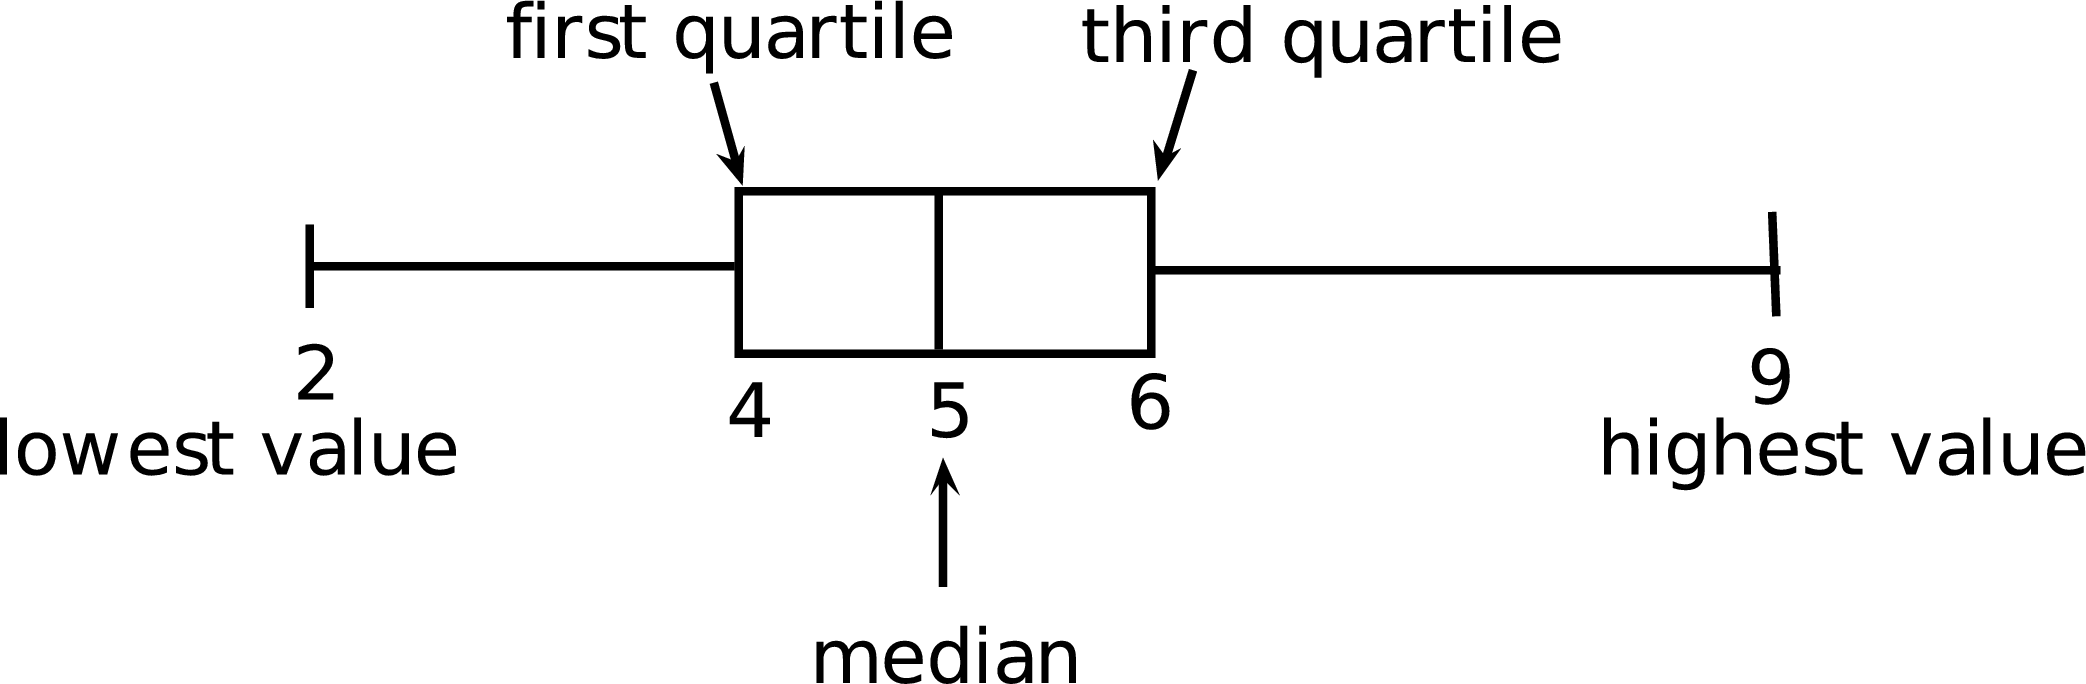
\includegraphics[width=300px]{col11306.imgs/m39400_boxwhisker.png} % m39400;boxwhisker.png;;;6.0;8.5;
      \vspace{2pt}
    \vspace{\rubberspace}\par \begin{cnxcaption}
	  \small \textbf{Figure 16.4: }Main features of a box and whisker plot
	\end{cnxcaption}
    \vspace{.1in}
    \end{center}
 \end{figure}       \par \par
            \label{m39400*eip-742}\vspace{.5cm} 
      \noindent
      \hspace*{-30pt}
\includegraphics[width=0.5in]{col11306.imgs/pspencil2.png}   \raisebox{25mm}{   
      \begin{mdframed}[linewidth=4, leftmargin=40, rightmargin=40]  
      \begin{exercise}
    \noindent\textbf{Exercise 16.9}\label{m39400*eip-570}
  \label{m39400*eip-327}
Draw a box and whisker diagram for the data set:
\begin{math}x=\{1,25;1,5;2,5;2,5;3,1;3,2;4,1;4,25;4,75;4,8;4,95;5,1\}\end{math}.
  \par 
\vspace{5pt}
\label{m39400*eip-402}\noindent\textbf{Solution to Exercise }
  \label{m39400*eip-701}\begin{enumerate}[noitemsep, label=\textbf{Step} \textbf{\arabic*}. ] 
            \leftskip=20pt\rightskip=\leftskip\item \newline
    \begin{math}\mathrm{Minimum}=1,25\end{math}\newline
\begin{math}\mathrm{Maximum}=5,10\end{math}\newline
The position of first quartile is between 3 and 4. \newline
The position of second quartile is between 6 and 7. \newline
The position of third quartile is between 9 and 10. \newline
The data value between 3 and 4 is:
\begin{math}\frac{1}{2}\left(2,5+2,5\right)=2,5\end{math}\newline
The data value between 6 and 7 is:
\begin{math}\frac{1}{2}\left(3,2+4,1\right)=3,65\end{math}\newline
The data value between 9 and 10 is: 
\begin{math}\frac{1}{2}\left(4,75+4,8\right)=4,775\end{math}\item 
    \setcounter{subfigure}{0}
	\begin{figure}[H] % horizontal\label{m39400*uid34553}
    \begin{center}
    \label{m39400*uid34553!!!underscore!!!media}\label{m39400*uid34553!!!underscore!!!printimage}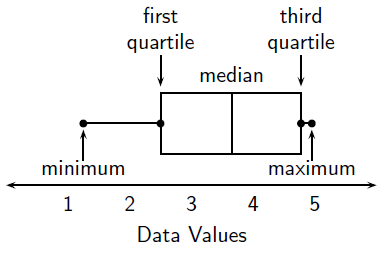
\includegraphics{col11306.imgs/m39400_boxwhisker1.png} % ;boxwhisker1.png;;;6.0;8.5;
      \vspace{2pt}
    \vspace{.1in}
    \end{center}
 \end{figure}       \end{enumerate}
    \end{exercise}
    \end{mdframed}
    }
    \noindent
  \label{m39400*uid86}
            \subsubsection{ Exercises - Summarising Data}
            \nopagebreak
        \label{m39400*id214700}\begin{enumerate}[noitemsep, label=\textbf{\arabic*}. ] 
            \label{m39400*uid87}\item Three sets of data are given:
\label{m39400*id214716}\begin{enumerate}[noitemsep, label=\textbf{\alph*}. ] 
            \label{m39400*uid88}\item \textbf{Data set 1:} 9 12 12 14 16 22 24
\label{m39400*uid89}\item \textbf{Data set 2:} 7 7 8 11 13 15 16 16
\label{m39400*uid90}\item \textbf{Data set 3:} 11 15 16 17 19 19 22 24 27\end{enumerate}
For each one find:
\label{m39400*id214775}\begin{enumerate}[noitemsep, label=\textbf{\alph*}. ] 
            \label{m39400*uid91}\item the range
\label{m39400*uid92}\item the lower quartile
\label{m39400*uid93}\item the interquartile range
\label{m39400*uid94}\item the semi-interquartile range
\label{m39400*uid95}\item the median
\label{m39400*uid96}\item the upper quartile
\end{enumerate}
                \label{m39400*uid97}\item There is 1 sweet in one jar, and 3 in the second jar. The mean number of sweets in the first two jars is 2.
\label{m39400*id214868}\begin{enumerate}[noitemsep, label=\textbf{\alph*}. ] 
            \label{m39400*uid98}\item If the mean number in the first three jars is 3, how many are there in the third jar?
\label{m39400*uid99}\item If the mean number in the first four jars is 4, how many are there in the fourth jar?
\end{enumerate}
                \label{m39400*uid101}\item Find a set of five ages for which the mean age is 5, the modal age is 2 and the median age is 3 years.\newline
\label{m39400*uid102}\item Four friends each have some marbles. They work out that the mean number of marbles they have is 10. One of them leaves. She has 4 marbles. How many marbles do the remaining friends have together?\newline
\item Jason is working in a computer store. He sells the following number of computers each month:
27; 39; 3; 15; 43; 27; 19; 54; 65; 23; 45; 16
Give a five number summary and a box and whisker plot of his sales.\newline
\item Lisa works as a telesales person. She keeps a record of the number of sales she makes each month. The data below show how much she sells each month.
49; 12; 22; 35; 2; 45; 60; 48; 19; 1; 43; 12
Give a five number summary and a box and whisker plot of her sales.\newline
\item Rose has worked in a florists shop for nine months. She sold the following number of wedding bouquets:
16; 14; 8; 12; 6; 5; 3; 5; 7
\label{m39400*id63452}\begin{enumerate}[noitemsep, label=\textbf{\alph*}. ] 
            \item What is the five-number summary of the data?\item Since there is an odd number of data points what do you observe when calculating the five-numbers?\end{enumerate}
\end{enumerate}
\label{m39400*eip-405}We can apply the concepts of mean, median and mode to data that has been grouped. Grouped data does not have individual data points, but rather has the data organized into groups or bins. To calculate the mean we need to add up all the frequencies and divide by the total. We do not know what the actual data values are, so we approximate by choosing the midpoint of each group. We then multiply those midpoint numbers by the frequency. Then we add these numbers together to find the approximate total of the masses. The modal group is the group with the highest frequency. The median group is the group that contains the middle terms.\par \label{m39400*eip-151}Measures of dispersion can also be found for grouped data. The range is found by subtracting the smallest number in the lowest bin from the largest number in the highest bin. The quartiles are found in a similar way to the median.\par \label{m39400*secfhsst!!!underscore!!!id2004}\vspace{.5cm} 
      \noindent
      \hspace*{-30pt}
\includegraphics[width=0.5in]{col11306.imgs/pspencil2.png}   \raisebox{25mm}{   
      \begin{mdframed}[linewidth=4, leftmargin=40, rightmargin=40]  
      \begin{exercise}
    \noindent\textbf{Exercise 16.10:  Mean, Median and Mode for Grouped Data }
        \label{m39400*probfhsst!!!underscore!!!id2005}
        \label{m39400*id214977}Consider the following grouped data and calculate the mean, the modal group and the median group.\par 
    % \textbf{m39400*id214984}\par
    % how many colspecs?  2
          % name: cnx:colspec
            % colnum: 1
            % colwidth: 10*
            % latex-name: columna
            % colname: 
            % align/tgroup-align/default: //left
            % -------------------------
            % name: cnx:colspec
            % colnum: 2
            % colwidth: 10*
            % latex-name: columnb
            % colname: 
            % align/tgroup-align/default: //left
            % -------------------------
    \setlength\mytablespace{4\tabcolsep}
    \addtolength\mytablespace{3\arrayrulewidth}
    \setlength\mytablewidth{\linewidth}
    \setlength\mytableroom{\mytablewidth}
    \addtolength\mytableroom{-\mytablespace}
    \setlength\myfixedwidth{0pt}
    \setlength\mystarwidth{\mytableroom}
        \addtolength\mystarwidth{-\myfixedwidth}
        \divide\mystarwidth 20
      % ----- Begin capturing width of table in LR mode woof
      \settowidth{\mytableboxwidth}{\begin{tabular}[t]{|l|l|}\hline
    % count in rowspan-info-nodeset: 2
    % align/colidx: left,1
    % rowcount: '0' | start: 'false' | colidx: '1'
        % Formatting a regular cell and recurring on the next sibling
        Mass (kg) &
      % align/colidx: left,2
    % rowcount: '0' | start: 'false' | colidx: '2'
        % Formatting a regular cell and recurring on the next sibling
        Frequency% make-rowspan-placeholders
    % rowspan info: col1 '0' | 'false' | '' || col2 '0' | 'false' | ''
     \tabularnewline\cline{1-1}\cline{2-2}
      %--------------------------------------------------------------------
    % align/colidx: left,1
    % rowcount: '0' | start: 'false' | colidx: '1'
        % Formatting a regular cell and recurring on the next sibling
        41 - 45 &
      % align/colidx: left,2
    % rowcount: '0' | start: 'false' | colidx: '2'
        % Formatting a regular cell and recurring on the next sibling
        7% make-rowspan-placeholders
    % rowspan info: col1 '0' | 'false' | '' || col2 '0' | 'false' | ''
     \tabularnewline\cline{1-1}\cline{2-2}
      %--------------------------------------------------------------------
    % align/colidx: left,1
    % rowcount: '0' | start: 'false' | colidx: '1'
        % Formatting a regular cell and recurring on the next sibling
        46 - 50 &
      % align/colidx: left,2
    % rowcount: '0' | start: 'false' | colidx: '2'
        % Formatting a regular cell and recurring on the next sibling
        10% make-rowspan-placeholders
    % rowspan info: col1 '0' | 'false' | '' || col2 '0' | 'false' | ''
     \tabularnewline\cline{1-1}\cline{2-2}
      %--------------------------------------------------------------------
    % align/colidx: left,1
    % rowcount: '0' | start: 'false' | colidx: '1'
        % Formatting a regular cell and recurring on the next sibling
        51 - 55 &
      % align/colidx: left,2
    % rowcount: '0' | start: 'false' | colidx: '2'
        % Formatting a regular cell and recurring on the next sibling
        15% make-rowspan-placeholders
    % rowspan info: col1 '0' | 'false' | '' || col2 '0' | 'false' | ''
     \tabularnewline\cline{1-1}\cline{2-2}
      %--------------------------------------------------------------------
    % align/colidx: left,1
    % rowcount: '0' | start: 'false' | colidx: '1'
        % Formatting a regular cell and recurring on the next sibling
        56 - 60 &
      % align/colidx: left,2
    % rowcount: '0' | start: 'false' | colidx: '2'
        % Formatting a regular cell and recurring on the next sibling
        12% make-rowspan-placeholders
    % rowspan info: col1 '0' | 'false' | '' || col2 '0' | 'false' | ''
     \tabularnewline\cline{1-1}\cline{2-2}
      %--------------------------------------------------------------------
    % align/colidx: left,1
    % rowcount: '0' | start: 'false' | colidx: '1'
        % Formatting a regular cell and recurring on the next sibling
        61 - 65 &
      % align/colidx: left,2
    % rowcount: '0' | start: 'false' | colidx: '2'
        % Formatting a regular cell and recurring on the next sibling
        6% make-rowspan-placeholders
    % rowspan info: col1 '0' | 'false' | '' || col2 '0' | 'false' | ''
     \tabularnewline\cline{1-1}\cline{2-2}
      %--------------------------------------------------------------------
    % align/colidx: left,1
    % rowcount: '0' | start: 'false' | colidx: '1'
        % Formatting a regular cell and recurring on the next sibling
         &
      % align/colidx: left,2
    % rowcount: '0' | start: 'false' | colidx: '2'
        % Formatting a regular cell and recurring on the next sibling
        Total = 50% make-rowspan-placeholders
    % rowspan info: col1 '0' | 'false' | '' || col2 '0' | 'false' | ''
     \tabularnewline\cline{1-1}\cline{2-2}
      %--------------------------------------------------------------------
    \end{tabular}} % end mytableboxwidth set      
      % ----- End capturing width of table in LR mode
        % ----- LR or paragraph mode: must test
        % ----- Begin capturing height of table
        \settoheight{\mytableboxheight}{\begin{tabular}[t]{|l|l|}\hline
    % count in rowspan-info-nodeset: 2
    % align/colidx: left,1
    % rowcount: '0' | start: 'false' | colidx: '1'
        % Formatting a regular cell and recurring on the next sibling
        Mass (kg) &
      % align/colidx: left,2
    % rowcount: '0' | start: 'false' | colidx: '2'
        % Formatting a regular cell and recurring on the next sibling
        Frequency% make-rowspan-placeholders
    % rowspan info: col1 '0' | 'false' | '' || col2 '0' | 'false' | ''
     \tabularnewline\cline{1-1}\cline{2-2}
      %--------------------------------------------------------------------
    % align/colidx: left,1
    % rowcount: '0' | start: 'false' | colidx: '1'
        % Formatting a regular cell and recurring on the next sibling
        41 - 45 &
      % align/colidx: left,2
    % rowcount: '0' | start: 'false' | colidx: '2'
        % Formatting a regular cell and recurring on the next sibling
        7% make-rowspan-placeholders
    % rowspan info: col1 '0' | 'false' | '' || col2 '0' | 'false' | ''
     \tabularnewline\cline{1-1}\cline{2-2}
      %--------------------------------------------------------------------
    % align/colidx: left,1
    % rowcount: '0' | start: 'false' | colidx: '1'
        % Formatting a regular cell and recurring on the next sibling
        46 - 50 &
      % align/colidx: left,2
    % rowcount: '0' | start: 'false' | colidx: '2'
        % Formatting a regular cell and recurring on the next sibling
        10% make-rowspan-placeholders
    % rowspan info: col1 '0' | 'false' | '' || col2 '0' | 'false' | ''
     \tabularnewline\cline{1-1}\cline{2-2}
      %--------------------------------------------------------------------
    % align/colidx: left,1
    % rowcount: '0' | start: 'false' | colidx: '1'
        % Formatting a regular cell and recurring on the next sibling
        51 - 55 &
      % align/colidx: left,2
    % rowcount: '0' | start: 'false' | colidx: '2'
        % Formatting a regular cell and recurring on the next sibling
        15% make-rowspan-placeholders
    % rowspan info: col1 '0' | 'false' | '' || col2 '0' | 'false' | ''
     \tabularnewline\cline{1-1}\cline{2-2}
      %--------------------------------------------------------------------
    % align/colidx: left,1
    % rowcount: '0' | start: 'false' | colidx: '1'
        % Formatting a regular cell and recurring on the next sibling
        56 - 60 &
      % align/colidx: left,2
    % rowcount: '0' | start: 'false' | colidx: '2'
        % Formatting a regular cell and recurring on the next sibling
        12% make-rowspan-placeholders
    % rowspan info: col1 '0' | 'false' | '' || col2 '0' | 'false' | ''
     \tabularnewline\cline{1-1}\cline{2-2}
      %--------------------------------------------------------------------
    % align/colidx: left,1
    % rowcount: '0' | start: 'false' | colidx: '1'
        % Formatting a regular cell and recurring on the next sibling
        61 - 65 &
      % align/colidx: left,2
    % rowcount: '0' | start: 'false' | colidx: '2'
        % Formatting a regular cell and recurring on the next sibling
        6% make-rowspan-placeholders
    % rowspan info: col1 '0' | 'false' | '' || col2 '0' | 'false' | ''
     \tabularnewline\cline{1-1}\cline{2-2}
      %--------------------------------------------------------------------
    % align/colidx: left,1
    % rowcount: '0' | start: 'false' | colidx: '1'
        % Formatting a regular cell and recurring on the next sibling
         &
      % align/colidx: left,2
    % rowcount: '0' | start: 'false' | colidx: '2'
        % Formatting a regular cell and recurring on the next sibling
        Total = 50% make-rowspan-placeholders
    % rowspan info: col1 '0' | 'false' | '' || col2 '0' | 'false' | ''
     \tabularnewline\cline{1-1}\cline{2-2}
      %--------------------------------------------------------------------
    \end{tabular}} % end mytableboxheight set
        \settodepth{\mytableboxdepth}{\begin{tabular}[t]{|l|l|}\hline
    % count in rowspan-info-nodeset: 2
    % align/colidx: left,1
    % rowcount: '0' | start: 'false' | colidx: '1'
        % Formatting a regular cell and recurring on the next sibling
        Mass (kg) &
      % align/colidx: left,2
    % rowcount: '0' | start: 'false' | colidx: '2'
        % Formatting a regular cell and recurring on the next sibling
        Frequency% make-rowspan-placeholders
    % rowspan info: col1 '0' | 'false' | '' || col2 '0' | 'false' | ''
     \tabularnewline\cline{1-1}\cline{2-2}
      %--------------------------------------------------------------------
    % align/colidx: left,1
    % rowcount: '0' | start: 'false' | colidx: '1'
        % Formatting a regular cell and recurring on the next sibling
        41 - 45 &
      % align/colidx: left,2
    % rowcount: '0' | start: 'false' | colidx: '2'
        % Formatting a regular cell and recurring on the next sibling
        7% make-rowspan-placeholders
    % rowspan info: col1 '0' | 'false' | '' || col2 '0' | 'false' | ''
     \tabularnewline\cline{1-1}\cline{2-2}
      %--------------------------------------------------------------------
    % align/colidx: left,1
    % rowcount: '0' | start: 'false' | colidx: '1'
        % Formatting a regular cell and recurring on the next sibling
        46 - 50 &
      % align/colidx: left,2
    % rowcount: '0' | start: 'false' | colidx: '2'
        % Formatting a regular cell and recurring on the next sibling
        10% make-rowspan-placeholders
    % rowspan info: col1 '0' | 'false' | '' || col2 '0' | 'false' | ''
     \tabularnewline\cline{1-1}\cline{2-2}
      %--------------------------------------------------------------------
    % align/colidx: left,1
    % rowcount: '0' | start: 'false' | colidx: '1'
        % Formatting a regular cell and recurring on the next sibling
        51 - 55 &
      % align/colidx: left,2
    % rowcount: '0' | start: 'false' | colidx: '2'
        % Formatting a regular cell and recurring on the next sibling
        15% make-rowspan-placeholders
    % rowspan info: col1 '0' | 'false' | '' || col2 '0' | 'false' | ''
     \tabularnewline\cline{1-1}\cline{2-2}
      %--------------------------------------------------------------------
    % align/colidx: left,1
    % rowcount: '0' | start: 'false' | colidx: '1'
        % Formatting a regular cell and recurring on the next sibling
        56 - 60 &
      % align/colidx: left,2
    % rowcount: '0' | start: 'false' | colidx: '2'
        % Formatting a regular cell and recurring on the next sibling
        12% make-rowspan-placeholders
    % rowspan info: col1 '0' | 'false' | '' || col2 '0' | 'false' | ''
     \tabularnewline\cline{1-1}\cline{2-2}
      %--------------------------------------------------------------------
    % align/colidx: left,1
    % rowcount: '0' | start: 'false' | colidx: '1'
        % Formatting a regular cell and recurring on the next sibling
        61 - 65 &
      % align/colidx: left,2
    % rowcount: '0' | start: 'false' | colidx: '2'
        % Formatting a regular cell and recurring on the next sibling
        6% make-rowspan-placeholders
    % rowspan info: col1 '0' | 'false' | '' || col2 '0' | 'false' | ''
     \tabularnewline\cline{1-1}\cline{2-2}
      %--------------------------------------------------------------------
    % align/colidx: left,1
    % rowcount: '0' | start: 'false' | colidx: '1'
        % Formatting a regular cell and recurring on the next sibling
         &
      % align/colidx: left,2
    % rowcount: '0' | start: 'false' | colidx: '2'
        % Formatting a regular cell and recurring on the next sibling
        Total = 50% make-rowspan-placeholders
    % rowspan info: col1 '0' | 'false' | '' || col2 '0' | 'false' | ''
     \tabularnewline\cline{1-1}\cline{2-2}
      %--------------------------------------------------------------------
    \end{tabular}} % end mytableboxdepth set
        \addtolength{\mytableboxheight}{\mytableboxdepth}
        % ----- End capturing height of table        
        \ifthenelse{\mytableboxwidth<\textwidth}{% the table fits in LR mode
          \addtolength{\mytableboxwidth}{-\mytablespace}
          \typeout{textheight: \the\textheight}
          \typeout{mytableboxheight: \the\mytableboxheight}
          \typeout{textwidth: \the\textwidth}
          \typeout{mytableboxwidth: \the\mytableboxwidth}
          \ifthenelse{\mytableboxheight<\textheight}{%
    % \begin{table}[H]
    % \\ '' '0'
        \begin{center}
      \label{m39400*id214984}
    \noindent
    \begin{tabular}[t]{|l|l|}\hline
    % count in rowspan-info-nodeset: 2
    % align/colidx: left,1
    % rowcount: '0' | start: 'false' | colidx: '1'
        % Formatting a regular cell and recurring on the next sibling
        Mass (kg) &
      % align/colidx: left,2
    % rowcount: '0' | start: 'false' | colidx: '2'
        % Formatting a regular cell and recurring on the next sibling
        Frequency% make-rowspan-placeholders
    % rowspan info: col1 '0' | 'false' | '' || col2 '0' | 'false' | ''
     \tabularnewline\cline{1-1}\cline{2-2}
      %--------------------------------------------------------------------
    % align/colidx: left,1
    % rowcount: '0' | start: 'false' | colidx: '1'
        % Formatting a regular cell and recurring on the next sibling
        41 - 45 &
      % align/colidx: left,2
    % rowcount: '0' | start: 'false' | colidx: '2'
        % Formatting a regular cell and recurring on the next sibling
        7% make-rowspan-placeholders
    % rowspan info: col1 '0' | 'false' | '' || col2 '0' | 'false' | ''
     \tabularnewline\cline{1-1}\cline{2-2}
      %--------------------------------------------------------------------
    % align/colidx: left,1
    % rowcount: '0' | start: 'false' | colidx: '1'
        % Formatting a regular cell and recurring on the next sibling
        46 - 50 &
      % align/colidx: left,2
    % rowcount: '0' | start: 'false' | colidx: '2'
        % Formatting a regular cell and recurring on the next sibling
        10% make-rowspan-placeholders
    % rowspan info: col1 '0' | 'false' | '' || col2 '0' | 'false' | ''
     \tabularnewline\cline{1-1}\cline{2-2}
      %--------------------------------------------------------------------
    % align/colidx: left,1
    % rowcount: '0' | start: 'false' | colidx: '1'
        % Formatting a regular cell and recurring on the next sibling
        51 - 55 &
      % align/colidx: left,2
    % rowcount: '0' | start: 'false' | colidx: '2'
        % Formatting a regular cell and recurring on the next sibling
        15% make-rowspan-placeholders
    % rowspan info: col1 '0' | 'false' | '' || col2 '0' | 'false' | ''
     \tabularnewline\cline{1-1}\cline{2-2}
      %--------------------------------------------------------------------
    % align/colidx: left,1
    % rowcount: '0' | start: 'false' | colidx: '1'
        % Formatting a regular cell and recurring on the next sibling
        56 - 60 &
      % align/colidx: left,2
    % rowcount: '0' | start: 'false' | colidx: '2'
        % Formatting a regular cell and recurring on the next sibling
        12% make-rowspan-placeholders
    % rowspan info: col1 '0' | 'false' | '' || col2 '0' | 'false' | ''
     \tabularnewline\cline{1-1}\cline{2-2}
      %--------------------------------------------------------------------
    % align/colidx: left,1
    % rowcount: '0' | start: 'false' | colidx: '1'
        % Formatting a regular cell and recurring on the next sibling
        61 - 65 &
      % align/colidx: left,2
    % rowcount: '0' | start: 'false' | colidx: '2'
        % Formatting a regular cell and recurring on the next sibling
        6% make-rowspan-placeholders
    % rowspan info: col1 '0' | 'false' | '' || col2 '0' | 'false' | ''
     \tabularnewline\cline{1-1}\cline{2-2}
      %--------------------------------------------------------------------
    % align/colidx: left,1
    % rowcount: '0' | start: 'false' | colidx: '1'
        % Formatting a regular cell and recurring on the next sibling
         &
      % align/colidx: left,2
    % rowcount: '0' | start: 'false' | colidx: '2'
        % Formatting a regular cell and recurring on the next sibling
        Total = 50% make-rowspan-placeholders
    % rowspan info: col1 '0' | 'false' | '' || col2 '0' | 'false' | ''
     \tabularnewline\cline{1-1}\cline{2-2}
      %--------------------------------------------------------------------
    \end{tabular}
      \end{center}
    \begin{center}{\small\bfseries Table 16.14}\end{center}
    %\end{table}
          }{ % else
    % \begin{table}[H]
    % \\ '' '0'
        \begin{center}
      \label{m39400*id214984}
    \noindent
    \tabletail{%
        \hline
        \multicolumn{2}{|p{\mytableboxwidth}|}{\raggedleft \small \sl continued on next page}\\
        \hline
      }
      \tablelasttail{}
      \begin{xtabular}[t]{|l|l|}\hline
    % count in rowspan-info-nodeset: 2
    % align/colidx: left,1
    % rowcount: '0' | start: 'false' | colidx: '1'
        % Formatting a regular cell and recurring on the next sibling
        Mass (kg) &
      % align/colidx: left,2
    % rowcount: '0' | start: 'false' | colidx: '2'
        % Formatting a regular cell and recurring on the next sibling
        Frequency% make-rowspan-placeholders
    % rowspan info: col1 '0' | 'false' | '' || col2 '0' | 'false' | ''
     \tabularnewline\cline{1-1}\cline{2-2}
      %--------------------------------------------------------------------
    % align/colidx: left,1
    % rowcount: '0' | start: 'false' | colidx: '1'
        % Formatting a regular cell and recurring on the next sibling
        41 - 45 &
      % align/colidx: left,2
    % rowcount: '0' | start: 'false' | colidx: '2'
        % Formatting a regular cell and recurring on the next sibling
        7% make-rowspan-placeholders
    % rowspan info: col1 '0' | 'false' | '' || col2 '0' | 'false' | ''
     \tabularnewline\cline{1-1}\cline{2-2}
      %--------------------------------------------------------------------
    % align/colidx: left,1
    % rowcount: '0' | start: 'false' | colidx: '1'
        % Formatting a regular cell and recurring on the next sibling
        46 - 50 &
      % align/colidx: left,2
    % rowcount: '0' | start: 'false' | colidx: '2'
        % Formatting a regular cell and recurring on the next sibling
        10% make-rowspan-placeholders
    % rowspan info: col1 '0' | 'false' | '' || col2 '0' | 'false' | ''
     \tabularnewline\cline{1-1}\cline{2-2}
      %--------------------------------------------------------------------
    % align/colidx: left,1
    % rowcount: '0' | start: 'false' | colidx: '1'
        % Formatting a regular cell and recurring on the next sibling
        51 - 55 &
      % align/colidx: left,2
    % rowcount: '0' | start: 'false' | colidx: '2'
        % Formatting a regular cell and recurring on the next sibling
        15% make-rowspan-placeholders
    % rowspan info: col1 '0' | 'false' | '' || col2 '0' | 'false' | ''
     \tabularnewline\cline{1-1}\cline{2-2}
      %--------------------------------------------------------------------
    % align/colidx: left,1
    % rowcount: '0' | start: 'false' | colidx: '1'
        % Formatting a regular cell and recurring on the next sibling
        56 - 60 &
      % align/colidx: left,2
    % rowcount: '0' | start: 'false' | colidx: '2'
        % Formatting a regular cell and recurring on the next sibling
        12% make-rowspan-placeholders
    % rowspan info: col1 '0' | 'false' | '' || col2 '0' | 'false' | ''
     \tabularnewline\cline{1-1}\cline{2-2}
      %--------------------------------------------------------------------
    % align/colidx: left,1
    % rowcount: '0' | start: 'false' | colidx: '1'
        % Formatting a regular cell and recurring on the next sibling
        61 - 65 &
      % align/colidx: left,2
    % rowcount: '0' | start: 'false' | colidx: '2'
        % Formatting a regular cell and recurring on the next sibling
        6% make-rowspan-placeholders
    % rowspan info: col1 '0' | 'false' | '' || col2 '0' | 'false' | ''
     \tabularnewline\cline{1-1}\cline{2-2}
      %--------------------------------------------------------------------
    % align/colidx: left,1
    % rowcount: '0' | start: 'false' | colidx: '1'
        % Formatting a regular cell and recurring on the next sibling
         &
      % align/colidx: left,2
    % rowcount: '0' | start: 'false' | colidx: '2'
        % Formatting a regular cell and recurring on the next sibling
        Total = 50% make-rowspan-placeholders
    % rowspan info: col1 '0' | 'false' | '' || col2 '0' | 'false' | ''
     \tabularnewline\cline{1-1}\cline{2-2}
      %--------------------------------------------------------------------
    \end{xtabular}
      \end{center}
    \begin{center}{\small\bfseries Table 16.14}\end{center}
    %\end{table}
          } % 
        }{% else
        % typeset the table in paragraph mode
        % ----- Begin capturing height of table
        \settoheight{\mytableboxheight}{\begin{tabular*}{\mytablewidth}[t]{|p{10\mystarwidth}|p{10\mystarwidth}|}\hline
    % count in rowspan-info-nodeset: 2
    % align/colidx: left,1
    % rowcount: '0' | start: 'false' | colidx: '1'
        % Formatting a regular cell and recurring on the next sibling
        Mass (kg) &
      % align/colidx: left,2
    % rowcount: '0' | start: 'false' | colidx: '2'
        % Formatting a regular cell and recurring on the next sibling
        Frequency% make-rowspan-placeholders
    % rowspan info: col1 '0' | 'false' | '' || col2 '0' | 'false' | ''
     \tabularnewline\cline{1-1}\cline{2-2}
      %--------------------------------------------------------------------
    % align/colidx: left,1
    % rowcount: '0' | start: 'false' | colidx: '1'
        % Formatting a regular cell and recurring on the next sibling
        41 - 45 &
      % align/colidx: left,2
    % rowcount: '0' | start: 'false' | colidx: '2'
        % Formatting a regular cell and recurring on the next sibling
        7% make-rowspan-placeholders
    % rowspan info: col1 '0' | 'false' | '' || col2 '0' | 'false' | ''
     \tabularnewline\cline{1-1}\cline{2-2}
      %--------------------------------------------------------------------
    % align/colidx: left,1
    % rowcount: '0' | start: 'false' | colidx: '1'
        % Formatting a regular cell and recurring on the next sibling
        46 - 50 &
      % align/colidx: left,2
    % rowcount: '0' | start: 'false' | colidx: '2'
        % Formatting a regular cell and recurring on the next sibling
        10% make-rowspan-placeholders
    % rowspan info: col1 '0' | 'false' | '' || col2 '0' | 'false' | ''
     \tabularnewline\cline{1-1}\cline{2-2}
      %--------------------------------------------------------------------
    % align/colidx: left,1
    % rowcount: '0' | start: 'false' | colidx: '1'
        % Formatting a regular cell and recurring on the next sibling
        51 - 55 &
      % align/colidx: left,2
    % rowcount: '0' | start: 'false' | colidx: '2'
        % Formatting a regular cell and recurring on the next sibling
        15% make-rowspan-placeholders
    % rowspan info: col1 '0' | 'false' | '' || col2 '0' | 'false' | ''
     \tabularnewline\cline{1-1}\cline{2-2}
      %--------------------------------------------------------------------
    % align/colidx: left,1
    % rowcount: '0' | start: 'false' | colidx: '1'
        % Formatting a regular cell and recurring on the next sibling
        56 - 60 &
      % align/colidx: left,2
    % rowcount: '0' | start: 'false' | colidx: '2'
        % Formatting a regular cell and recurring on the next sibling
        12% make-rowspan-placeholders
    % rowspan info: col1 '0' | 'false' | '' || col2 '0' | 'false' | ''
     \tabularnewline\cline{1-1}\cline{2-2}
      %--------------------------------------------------------------------
    % align/colidx: left,1
    % rowcount: '0' | start: 'false' | colidx: '1'
        % Formatting a regular cell and recurring on the next sibling
        61 - 65 &
      % align/colidx: left,2
    % rowcount: '0' | start: 'false' | colidx: '2'
        % Formatting a regular cell and recurring on the next sibling
        6% make-rowspan-placeholders
    % rowspan info: col1 '0' | 'false' | '' || col2 '0' | 'false' | ''
     \tabularnewline\cline{1-1}\cline{2-2}
      %--------------------------------------------------------------------
    % align/colidx: left,1
    % rowcount: '0' | start: 'false' | colidx: '1'
        % Formatting a regular cell and recurring on the next sibling
         &
      % align/colidx: left,2
    % rowcount: '0' | start: 'false' | colidx: '2'
        % Formatting a regular cell and recurring on the next sibling
        Total = 50% make-rowspan-placeholders
    % rowspan info: col1 '0' | 'false' | '' || col2 '0' | 'false' | ''
     \tabularnewline\cline{1-1}\cline{2-2}
      %--------------------------------------------------------------------
    \end{tabular*}} % end mytableboxheight set
        \settodepth{\mytableboxdepth}{\begin{tabular*}{\mytablewidth}[t]{|p{10\mystarwidth}|p{10\mystarwidth}|}\hline
    % count in rowspan-info-nodeset: 2
    % align/colidx: left,1
    % rowcount: '0' | start: 'false' | colidx: '1'
        % Formatting a regular cell and recurring on the next sibling
        Mass (kg) &
      % align/colidx: left,2
    % rowcount: '0' | start: 'false' | colidx: '2'
        % Formatting a regular cell and recurring on the next sibling
        Frequency% make-rowspan-placeholders
    % rowspan info: col1 '0' | 'false' | '' || col2 '0' | 'false' | ''
     \tabularnewline\cline{1-1}\cline{2-2}
      %--------------------------------------------------------------------
    % align/colidx: left,1
    % rowcount: '0' | start: 'false' | colidx: '1'
        % Formatting a regular cell and recurring on the next sibling
        41 - 45 &
      % align/colidx: left,2
    % rowcount: '0' | start: 'false' | colidx: '2'
        % Formatting a regular cell and recurring on the next sibling
        7% make-rowspan-placeholders
    % rowspan info: col1 '0' | 'false' | '' || col2 '0' | 'false' | ''
     \tabularnewline\cline{1-1}\cline{2-2}
      %--------------------------------------------------------------------
    % align/colidx: left,1
    % rowcount: '0' | start: 'false' | colidx: '1'
        % Formatting a regular cell and recurring on the next sibling
        46 - 50 &
      % align/colidx: left,2
    % rowcount: '0' | start: 'false' | colidx: '2'
        % Formatting a regular cell and recurring on the next sibling
        10% make-rowspan-placeholders
    % rowspan info: col1 '0' | 'false' | '' || col2 '0' | 'false' | ''
     \tabularnewline\cline{1-1}\cline{2-2}
      %--------------------------------------------------------------------
    % align/colidx: left,1
    % rowcount: '0' | start: 'false' | colidx: '1'
        % Formatting a regular cell and recurring on the next sibling
        51 - 55 &
      % align/colidx: left,2
    % rowcount: '0' | start: 'false' | colidx: '2'
        % Formatting a regular cell and recurring on the next sibling
        15% make-rowspan-placeholders
    % rowspan info: col1 '0' | 'false' | '' || col2 '0' | 'false' | ''
     \tabularnewline\cline{1-1}\cline{2-2}
      %--------------------------------------------------------------------
    % align/colidx: left,1
    % rowcount: '0' | start: 'false' | colidx: '1'
        % Formatting a regular cell and recurring on the next sibling
        56 - 60 &
      % align/colidx: left,2
    % rowcount: '0' | start: 'false' | colidx: '2'
        % Formatting a regular cell and recurring on the next sibling
        12% make-rowspan-placeholders
    % rowspan info: col1 '0' | 'false' | '' || col2 '0' | 'false' | ''
     \tabularnewline\cline{1-1}\cline{2-2}
      %--------------------------------------------------------------------
    % align/colidx: left,1
    % rowcount: '0' | start: 'false' | colidx: '1'
        % Formatting a regular cell and recurring on the next sibling
        61 - 65 &
      % align/colidx: left,2
    % rowcount: '0' | start: 'false' | colidx: '2'
        % Formatting a regular cell and recurring on the next sibling
        6% make-rowspan-placeholders
    % rowspan info: col1 '0' | 'false' | '' || col2 '0' | 'false' | ''
     \tabularnewline\cline{1-1}\cline{2-2}
      %--------------------------------------------------------------------
    % align/colidx: left,1
    % rowcount: '0' | start: 'false' | colidx: '1'
        % Formatting a regular cell and recurring on the next sibling
         &
      % align/colidx: left,2
    % rowcount: '0' | start: 'false' | colidx: '2'
        % Formatting a regular cell and recurring on the next sibling
        Total = 50% make-rowspan-placeholders
    % rowspan info: col1 '0' | 'false' | '' || col2 '0' | 'false' | ''
     \tabularnewline\cline{1-1}\cline{2-2}
      %--------------------------------------------------------------------
    \end{tabular*}} % end mytableboxdepth set
        \addtolength{\mytableboxheight}{\mytableboxdepth}
        % ----- End capturing height of table
        \typeout{textheight: \the\textheight}
        \typeout{mytableboxheight: \the\mytableboxheight}
        \typeout{table too wide, outputting in para mode}
    % \begin{table}[H]
    % \\ '' '0'
        \begin{center}
      \label{m39400*id214984}
    \noindent
    \tabletail{%
        \hline
        \multicolumn{2}{|p{\mytableroom}|}{\raggedleft \small \sl continued on next page}\\
        \hline
      }
      \tablelasttail{}
      \begin{xtabular*}{\mytablewidth}[t]{|p{10\mystarwidth}|p{10\mystarwidth}|}\hline
    % count in rowspan-info-nodeset: 2
    % align/colidx: left,1
    % rowcount: '0' | start: 'false' | colidx: '1'
        % Formatting a regular cell and recurring on the next sibling
        Mass (kg) &
      % align/colidx: left,2
    % rowcount: '0' | start: 'false' | colidx: '2'
        % Formatting a regular cell and recurring on the next sibling
        Frequency% make-rowspan-placeholders
    % rowspan info: col1 '0' | 'false' | '' || col2 '0' | 'false' | ''
     \tabularnewline\cline{1-1}\cline{2-2}
      %--------------------------------------------------------------------
    % align/colidx: left,1
    % rowcount: '0' | start: 'false' | colidx: '1'
        % Formatting a regular cell and recurring on the next sibling
        41 - 45 &
      % align/colidx: left,2
    % rowcount: '0' | start: 'false' | colidx: '2'
        % Formatting a regular cell and recurring on the next sibling
        7% make-rowspan-placeholders
    % rowspan info: col1 '0' | 'false' | '' || col2 '0' | 'false' | ''
     \tabularnewline\cline{1-1}\cline{2-2}
      %--------------------------------------------------------------------
    % align/colidx: left,1
    % rowcount: '0' | start: 'false' | colidx: '1'
        % Formatting a regular cell and recurring on the next sibling
        46 - 50 &
      % align/colidx: left,2
    % rowcount: '0' | start: 'false' | colidx: '2'
        % Formatting a regular cell and recurring on the next sibling
        10% make-rowspan-placeholders
    % rowspan info: col1 '0' | 'false' | '' || col2 '0' | 'false' | ''
     \tabularnewline\cline{1-1}\cline{2-2}
      %--------------------------------------------------------------------
    % align/colidx: left,1
    % rowcount: '0' | start: 'false' | colidx: '1'
        % Formatting a regular cell and recurring on the next sibling
        51 - 55 &
      % align/colidx: left,2
    % rowcount: '0' | start: 'false' | colidx: '2'
        % Formatting a regular cell and recurring on the next sibling
        15% make-rowspan-placeholders
    % rowspan info: col1 '0' | 'false' | '' || col2 '0' | 'false' | ''
     \tabularnewline\cline{1-1}\cline{2-2}
      %--------------------------------------------------------------------
    % align/colidx: left,1
    % rowcount: '0' | start: 'false' | colidx: '1'
        % Formatting a regular cell and recurring on the next sibling
        56 - 60 &
      % align/colidx: left,2
    % rowcount: '0' | start: 'false' | colidx: '2'
        % Formatting a regular cell and recurring on the next sibling
        12% make-rowspan-placeholders
    % rowspan info: col1 '0' | 'false' | '' || col2 '0' | 'false' | ''
     \tabularnewline\cline{1-1}\cline{2-2}
      %--------------------------------------------------------------------
    % align/colidx: left,1
    % rowcount: '0' | start: 'false' | colidx: '1'
        % Formatting a regular cell and recurring on the next sibling
        61 - 65 &
      % align/colidx: left,2
    % rowcount: '0' | start: 'false' | colidx: '2'
        % Formatting a regular cell and recurring on the next sibling
        6% make-rowspan-placeholders
    % rowspan info: col1 '0' | 'false' | '' || col2 '0' | 'false' | ''
     \tabularnewline\cline{1-1}\cline{2-2}
      %--------------------------------------------------------------------
    % align/colidx: left,1
    % rowcount: '0' | start: 'false' | colidx: '1'
        % Formatting a regular cell and recurring on the next sibling
         &
      % align/colidx: left,2
    % rowcount: '0' | start: 'false' | colidx: '2'
        % Formatting a regular cell and recurring on the next sibling
        Total = 50% make-rowspan-placeholders
    % rowspan info: col1 '0' | 'false' | '' || col2 '0' | 'false' | ''
     \tabularnewline\cline{1-1}\cline{2-2}
      %--------------------------------------------------------------------
    \end{xtabular*}
      \end{center}
    \begin{center}{\small\bfseries Table 16.14}\end{center}
    %\end{table}
        }% ending lr/para test clause
    \par
        \vspace{5pt}
        \label{m39400*solfhsst!!!underscore!!!id2044}\noindent\textbf{Solution to Exercise } \label{m39400*listfhsst!!!underscore!!!id2044}\begin{enumerate}[noitemsep, label=\textbf{Step} \textbf{\arabic*}. ] 
            \leftskip=20pt\rightskip=\leftskip\item  
        \label{m39400*id215169}To calculate the mean we need to add up all the masses and divide by 50. We do not know actual masses, so we approximate by choosing the midpoint of each group. We then multiply those midpoint numbers by the frequency. Then we add these numbers together to find the approximate total of the masses. This is show in the table below.\par 
    % \textbf{m39400*id215176}\par
    % how many colspecs?  4
          % name: cnx:colspec
            % colnum: 1
            % colwidth: 10*
            % latex-name: columna
            % colname: 
            % align/tgroup-align/default: //left
            % -------------------------
            % name: cnx:colspec
            % colnum: 2
            % colwidth: 10*
            % latex-name: columnb
            % colname: 
            % align/tgroup-align/default: //left
            % -------------------------
            % name: cnx:colspec
            % colnum: 3
            % colwidth: 10*
            % latex-name: columnc
            % colname: 
            % align/tgroup-align/default: //left
            % -------------------------
            % name: cnx:colspec
            % colnum: 4
            % colwidth: 10*
            % latex-name: columnd
            % colname: 
            % align/tgroup-align/default: //left
            % -------------------------
    \setlength\mytablespace{8\tabcolsep}
    \addtolength\mytablespace{5\arrayrulewidth}
    \setlength\mytablewidth{\linewidth}
    \setlength\mytableroom{\mytablewidth}
    \addtolength\mytableroom{-\mytablespace}
    \setlength\myfixedwidth{0pt}
    \setlength\mystarwidth{\mytableroom}
        \addtolength\mystarwidth{-\myfixedwidth}
        \divide\mystarwidth 40
      % ----- Begin capturing width of table in LR mode woof
      \settowidth{\mytableboxwidth}{\begin{tabular}[t]{|l|l|l|l|}\hline
    % count in rowspan-info-nodeset: 4
    % align/colidx: left,1
    % rowcount: '0' | start: 'false' | colidx: '1'
        % Formatting a regular cell and recurring on the next sibling
        Mass (kg) &
      % align/colidx: left,2
    % rowcount: '0' | start: 'false' | colidx: '2'
        % Formatting a regular cell and recurring on the next sibling
        Midpoint &
      % align/colidx: left,3
    % rowcount: '0' | start: 'false' | colidx: '3'
        % Formatting a regular cell and recurring on the next sibling
        Frequency &
      % align/colidx: left,4
    % rowcount: '0' | start: 'false' | colidx: '4'
        % Formatting a regular cell and recurring on the next sibling
        Midpt \begin{math}\ensuremath{\times}\end{math} Freq% make-rowspan-placeholders
    % rowspan info: col1 '0' | 'false' | '' || col2 '0' | 'false' | '' || col3 '0' | 'false' | '' || col4 '0' | 'false' | ''
     \tabularnewline\cline{1-1}\cline{2-2}\cline{3-3}\cline{4-4}
      %--------------------------------------------------------------------
    % align/colidx: left,1
    % rowcount: '0' | start: 'false' | colidx: '1'
        % Formatting a regular cell and recurring on the next sibling
        41 - 45 &
      % align/colidx: left,2
    % rowcount: '0' | start: 'false' | colidx: '2'
        % Formatting a regular cell and recurring on the next sibling
        (41+45)/2 = 43 &
      % align/colidx: left,3
    % rowcount: '0' | start: 'false' | colidx: '3'
        % Formatting a regular cell and recurring on the next sibling
        7 &
      % align/colidx: left,4
    % rowcount: '0' | start: 'false' | colidx: '4'
        % Formatting a regular cell and recurring on the next sibling
        43 \begin{math}\ensuremath{\times}\end{math} 7 = 301% make-rowspan-placeholders
    % rowspan info: col1 '0' | 'false' | '' || col2 '0' | 'false' | '' || col3 '0' | 'false' | '' || col4 '0' | 'false' | ''
     \tabularnewline\cline{1-1}\cline{2-2}\cline{3-3}\cline{4-4}
      %--------------------------------------------------------------------
    % align/colidx: left,1
    % rowcount: '0' | start: 'false' | colidx: '1'
        % Formatting a regular cell and recurring on the next sibling
        46 - 50 &
      % align/colidx: left,2
    % rowcount: '0' | start: 'false' | colidx: '2'
        % Formatting a regular cell and recurring on the next sibling
        48 &
      % align/colidx: left,3
    % rowcount: '0' | start: 'false' | colidx: '3'
        % Formatting a regular cell and recurring on the next sibling
        10 &
      % align/colidx: left,4
    % rowcount: '0' | start: 'false' | colidx: '4'
        % Formatting a regular cell and recurring on the next sibling
        480% make-rowspan-placeholders
    % rowspan info: col1 '0' | 'false' | '' || col2 '0' | 'false' | '' || col3 '0' | 'false' | '' || col4 '0' | 'false' | ''
     \tabularnewline\cline{1-1}\cline{2-2}\cline{3-3}\cline{4-4}
      %--------------------------------------------------------------------
    % align/colidx: left,1
    % rowcount: '0' | start: 'false' | colidx: '1'
        % Formatting a regular cell and recurring on the next sibling
        51 - 55 &
      % align/colidx: left,2
    % rowcount: '0' | start: 'false' | colidx: '2'
        % Formatting a regular cell and recurring on the next sibling
        53 &
      % align/colidx: left,3
    % rowcount: '0' | start: 'false' | colidx: '3'
        % Formatting a regular cell and recurring on the next sibling
        15 &
      % align/colidx: left,4
    % rowcount: '0' | start: 'false' | colidx: '4'
        % Formatting a regular cell and recurring on the next sibling
        795% make-rowspan-placeholders
    % rowspan info: col1 '0' | 'false' | '' || col2 '0' | 'false' | '' || col3 '0' | 'false' | '' || col4 '0' | 'false' | ''
     \tabularnewline\cline{1-1}\cline{2-2}\cline{3-3}\cline{4-4}
      %--------------------------------------------------------------------
    % align/colidx: left,1
    % rowcount: '0' | start: 'false' | colidx: '1'
        % Formatting a regular cell and recurring on the next sibling
        56 - 60 &
      % align/colidx: left,2
    % rowcount: '0' | start: 'false' | colidx: '2'
        % Formatting a regular cell and recurring on the next sibling
        58 &
      % align/colidx: left,3
    % rowcount: '0' | start: 'false' | colidx: '3'
        % Formatting a regular cell and recurring on the next sibling
        12 &
      % align/colidx: left,4
    % rowcount: '0' | start: 'false' | colidx: '4'
        % Formatting a regular cell and recurring on the next sibling
        696% make-rowspan-placeholders
    % rowspan info: col1 '0' | 'false' | '' || col2 '0' | 'false' | '' || col3 '0' | 'false' | '' || col4 '0' | 'false' | ''
     \tabularnewline\cline{1-1}\cline{2-2}\cline{3-3}\cline{4-4}
      %--------------------------------------------------------------------
    % align/colidx: left,1
    % rowcount: '0' | start: 'false' | colidx: '1'
        % Formatting a regular cell and recurring on the next sibling
        61 - 65 &
      % align/colidx: left,2
    % rowcount: '0' | start: 'false' | colidx: '2'
        % Formatting a regular cell and recurring on the next sibling
        63 &
      % align/colidx: left,3
    % rowcount: '0' | start: 'false' | colidx: '3'
        % Formatting a regular cell and recurring on the next sibling
        6 &
      % align/colidx: left,4
    % rowcount: '0' | start: 'false' | colidx: '4'
        % Formatting a regular cell and recurring on the next sibling
        378% make-rowspan-placeholders
    % rowspan info: col1 '0' | 'false' | '' || col2 '0' | 'false' | '' || col3 '0' | 'false' | '' || col4 '0' | 'false' | ''
     \tabularnewline\cline{1-1}\cline{2-2}\cline{3-3}\cline{4-4}
      %--------------------------------------------------------------------
    % align/colidx: left,1
    % rowcount: '0' | start: 'false' | colidx: '1'
        % Formatting a regular cell and recurring on the next sibling
         &
      % align/colidx: left,2
    % rowcount: '0' | start: 'false' | colidx: '2'
        % Formatting a regular cell and recurring on the next sibling
         &
      % align/colidx: left,3
    % rowcount: '0' | start: 'false' | colidx: '3'
        % Formatting a regular cell and recurring on the next sibling
        Total = 50 &
      % align/colidx: left,4
    % rowcount: '0' | start: 'false' | colidx: '4'
        % Formatting a regular cell and recurring on the next sibling
        Total = 2650% make-rowspan-placeholders
    % rowspan info: col1 '0' | 'false' | '' || col2 '0' | 'false' | '' || col3 '0' | 'false' | '' || col4 '0' | 'false' | ''
     \tabularnewline\cline{1-1}\cline{2-2}\cline{3-3}\cline{4-4}
      %--------------------------------------------------------------------
    \end{tabular}} % end mytableboxwidth set      
      % ----- End capturing width of table in LR mode
        % ----- LR or paragraph mode: must test
        % ----- Begin capturing height of table
        \settoheight{\mytableboxheight}{\begin{tabular}[t]{|l|l|l|l|}\hline
    % count in rowspan-info-nodeset: 4
    % align/colidx: left,1
    % rowcount: '0' | start: 'false' | colidx: '1'
        % Formatting a regular cell and recurring on the next sibling
        Mass (kg) &
      % align/colidx: left,2
    % rowcount: '0' | start: 'false' | colidx: '2'
        % Formatting a regular cell and recurring on the next sibling
        Midpoint &
      % align/colidx: left,3
    % rowcount: '0' | start: 'false' | colidx: '3'
        % Formatting a regular cell and recurring on the next sibling
        Frequency &
      % align/colidx: left,4
    % rowcount: '0' | start: 'false' | colidx: '4'
        % Formatting a regular cell and recurring on the next sibling
        Midpt \begin{math}\ensuremath{\times}\end{math} Freq% make-rowspan-placeholders
    % rowspan info: col1 '0' | 'false' | '' || col2 '0' | 'false' | '' || col3 '0' | 'false' | '' || col4 '0' | 'false' | ''
     \tabularnewline\cline{1-1}\cline{2-2}\cline{3-3}\cline{4-4}
      %--------------------------------------------------------------------
    % align/colidx: left,1
    % rowcount: '0' | start: 'false' | colidx: '1'
        % Formatting a regular cell and recurring on the next sibling
        41 - 45 &
      % align/colidx: left,2
    % rowcount: '0' | start: 'false' | colidx: '2'
        % Formatting a regular cell and recurring on the next sibling
        (41+45)/2 = 43 &
      % align/colidx: left,3
    % rowcount: '0' | start: 'false' | colidx: '3'
        % Formatting a regular cell and recurring on the next sibling
        7 &
      % align/colidx: left,4
    % rowcount: '0' | start: 'false' | colidx: '4'
        % Formatting a regular cell and recurring on the next sibling
        43 \begin{math}\ensuremath{\times}\end{math} 7 = 301% make-rowspan-placeholders
    % rowspan info: col1 '0' | 'false' | '' || col2 '0' | 'false' | '' || col3 '0' | 'false' | '' || col4 '0' | 'false' | ''
     \tabularnewline\cline{1-1}\cline{2-2}\cline{3-3}\cline{4-4}
      %--------------------------------------------------------------------
    % align/colidx: left,1
    % rowcount: '0' | start: 'false' | colidx: '1'
        % Formatting a regular cell and recurring on the next sibling
        46 - 50 &
      % align/colidx: left,2
    % rowcount: '0' | start: 'false' | colidx: '2'
        % Formatting a regular cell and recurring on the next sibling
        48 &
      % align/colidx: left,3
    % rowcount: '0' | start: 'false' | colidx: '3'
        % Formatting a regular cell and recurring on the next sibling
        10 &
      % align/colidx: left,4
    % rowcount: '0' | start: 'false' | colidx: '4'
        % Formatting a regular cell and recurring on the next sibling
        480% make-rowspan-placeholders
    % rowspan info: col1 '0' | 'false' | '' || col2 '0' | 'false' | '' || col3 '0' | 'false' | '' || col4 '0' | 'false' | ''
     \tabularnewline\cline{1-1}\cline{2-2}\cline{3-3}\cline{4-4}
      %--------------------------------------------------------------------
    % align/colidx: left,1
    % rowcount: '0' | start: 'false' | colidx: '1'
        % Formatting a regular cell and recurring on the next sibling
        51 - 55 &
      % align/colidx: left,2
    % rowcount: '0' | start: 'false' | colidx: '2'
        % Formatting a regular cell and recurring on the next sibling
        53 &
      % align/colidx: left,3
    % rowcount: '0' | start: 'false' | colidx: '3'
        % Formatting a regular cell and recurring on the next sibling
        15 &
      % align/colidx: left,4
    % rowcount: '0' | start: 'false' | colidx: '4'
        % Formatting a regular cell and recurring on the next sibling
        795% make-rowspan-placeholders
    % rowspan info: col1 '0' | 'false' | '' || col2 '0' | 'false' | '' || col3 '0' | 'false' | '' || col4 '0' | 'false' | ''
     \tabularnewline\cline{1-1}\cline{2-2}\cline{3-3}\cline{4-4}
      %--------------------------------------------------------------------
    % align/colidx: left,1
    % rowcount: '0' | start: 'false' | colidx: '1'
        % Formatting a regular cell and recurring on the next sibling
        56 - 60 &
      % align/colidx: left,2
    % rowcount: '0' | start: 'false' | colidx: '2'
        % Formatting a regular cell and recurring on the next sibling
        58 &
      % align/colidx: left,3
    % rowcount: '0' | start: 'false' | colidx: '3'
        % Formatting a regular cell and recurring on the next sibling
        12 &
      % align/colidx: left,4
    % rowcount: '0' | start: 'false' | colidx: '4'
        % Formatting a regular cell and recurring on the next sibling
        696% make-rowspan-placeholders
    % rowspan info: col1 '0' | 'false' | '' || col2 '0' | 'false' | '' || col3 '0' | 'false' | '' || col4 '0' | 'false' | ''
     \tabularnewline\cline{1-1}\cline{2-2}\cline{3-3}\cline{4-4}
      %--------------------------------------------------------------------
    % align/colidx: left,1
    % rowcount: '0' | start: 'false' | colidx: '1'
        % Formatting a regular cell and recurring on the next sibling
        61 - 65 &
      % align/colidx: left,2
    % rowcount: '0' | start: 'false' | colidx: '2'
        % Formatting a regular cell and recurring on the next sibling
        63 &
      % align/colidx: left,3
    % rowcount: '0' | start: 'false' | colidx: '3'
        % Formatting a regular cell and recurring on the next sibling
        6 &
      % align/colidx: left,4
    % rowcount: '0' | start: 'false' | colidx: '4'
        % Formatting a regular cell and recurring on the next sibling
        378% make-rowspan-placeholders
    % rowspan info: col1 '0' | 'false' | '' || col2 '0' | 'false' | '' || col3 '0' | 'false' | '' || col4 '0' | 'false' | ''
     \tabularnewline\cline{1-1}\cline{2-2}\cline{3-3}\cline{4-4}
      %--------------------------------------------------------------------
    % align/colidx: left,1
    % rowcount: '0' | start: 'false' | colidx: '1'
        % Formatting a regular cell and recurring on the next sibling
         &
      % align/colidx: left,2
    % rowcount: '0' | start: 'false' | colidx: '2'
        % Formatting a regular cell and recurring on the next sibling
         &
      % align/colidx: left,3
    % rowcount: '0' | start: 'false' | colidx: '3'
        % Formatting a regular cell and recurring on the next sibling
        Total = 50 &
      % align/colidx: left,4
    % rowcount: '0' | start: 'false' | colidx: '4'
        % Formatting a regular cell and recurring on the next sibling
        Total = 2650% make-rowspan-placeholders
    % rowspan info: col1 '0' | 'false' | '' || col2 '0' | 'false' | '' || col3 '0' | 'false' | '' || col4 '0' | 'false' | ''
     \tabularnewline\cline{1-1}\cline{2-2}\cline{3-3}\cline{4-4}
      %--------------------------------------------------------------------
    \end{tabular}} % end mytableboxheight set
        \settodepth{\mytableboxdepth}{\begin{tabular}[t]{|l|l|l|l|}\hline
    % count in rowspan-info-nodeset: 4
    % align/colidx: left,1
    % rowcount: '0' | start: 'false' | colidx: '1'
        % Formatting a regular cell and recurring on the next sibling
        Mass (kg) &
      % align/colidx: left,2
    % rowcount: '0' | start: 'false' | colidx: '2'
        % Formatting a regular cell and recurring on the next sibling
        Midpoint &
      % align/colidx: left,3
    % rowcount: '0' | start: 'false' | colidx: '3'
        % Formatting a regular cell and recurring on the next sibling
        Frequency &
      % align/colidx: left,4
    % rowcount: '0' | start: 'false' | colidx: '4'
        % Formatting a regular cell and recurring on the next sibling
        Midpt \begin{math}\ensuremath{\times}\end{math} Freq% make-rowspan-placeholders
    % rowspan info: col1 '0' | 'false' | '' || col2 '0' | 'false' | '' || col3 '0' | 'false' | '' || col4 '0' | 'false' | ''
     \tabularnewline\cline{1-1}\cline{2-2}\cline{3-3}\cline{4-4}
      %--------------------------------------------------------------------
    % align/colidx: left,1
    % rowcount: '0' | start: 'false' | colidx: '1'
        % Formatting a regular cell and recurring on the next sibling
        41 - 45 &
      % align/colidx: left,2
    % rowcount: '0' | start: 'false' | colidx: '2'
        % Formatting a regular cell and recurring on the next sibling
        (41+45)/2 = 43 &
      % align/colidx: left,3
    % rowcount: '0' | start: 'false' | colidx: '3'
        % Formatting a regular cell and recurring on the next sibling
        7 &
      % align/colidx: left,4
    % rowcount: '0' | start: 'false' | colidx: '4'
        % Formatting a regular cell and recurring on the next sibling
        43 \begin{math}\ensuremath{\times}\end{math} 7 = 301% make-rowspan-placeholders
    % rowspan info: col1 '0' | 'false' | '' || col2 '0' | 'false' | '' || col3 '0' | 'false' | '' || col4 '0' | 'false' | ''
     \tabularnewline\cline{1-1}\cline{2-2}\cline{3-3}\cline{4-4}
      %--------------------------------------------------------------------
    % align/colidx: left,1
    % rowcount: '0' | start: 'false' | colidx: '1'
        % Formatting a regular cell and recurring on the next sibling
        46 - 50 &
      % align/colidx: left,2
    % rowcount: '0' | start: 'false' | colidx: '2'
        % Formatting a regular cell and recurring on the next sibling
        48 &
      % align/colidx: left,3
    % rowcount: '0' | start: 'false' | colidx: '3'
        % Formatting a regular cell and recurring on the next sibling
        10 &
      % align/colidx: left,4
    % rowcount: '0' | start: 'false' | colidx: '4'
        % Formatting a regular cell and recurring on the next sibling
        480% make-rowspan-placeholders
    % rowspan info: col1 '0' | 'false' | '' || col2 '0' | 'false' | '' || col3 '0' | 'false' | '' || col4 '0' | 'false' | ''
     \tabularnewline\cline{1-1}\cline{2-2}\cline{3-3}\cline{4-4}
      %--------------------------------------------------------------------
    % align/colidx: left,1
    % rowcount: '0' | start: 'false' | colidx: '1'
        % Formatting a regular cell and recurring on the next sibling
        51 - 55 &
      % align/colidx: left,2
    % rowcount: '0' | start: 'false' | colidx: '2'
        % Formatting a regular cell and recurring on the next sibling
        53 &
      % align/colidx: left,3
    % rowcount: '0' | start: 'false' | colidx: '3'
        % Formatting a regular cell and recurring on the next sibling
        15 &
      % align/colidx: left,4
    % rowcount: '0' | start: 'false' | colidx: '4'
        % Formatting a regular cell and recurring on the next sibling
        795% make-rowspan-placeholders
    % rowspan info: col1 '0' | 'false' | '' || col2 '0' | 'false' | '' || col3 '0' | 'false' | '' || col4 '0' | 'false' | ''
     \tabularnewline\cline{1-1}\cline{2-2}\cline{3-3}\cline{4-4}
      %--------------------------------------------------------------------
    % align/colidx: left,1
    % rowcount: '0' | start: 'false' | colidx: '1'
        % Formatting a regular cell and recurring on the next sibling
        56 - 60 &
      % align/colidx: left,2
    % rowcount: '0' | start: 'false' | colidx: '2'
        % Formatting a regular cell and recurring on the next sibling
        58 &
      % align/colidx: left,3
    % rowcount: '0' | start: 'false' | colidx: '3'
        % Formatting a regular cell and recurring on the next sibling
        12 &
      % align/colidx: left,4
    % rowcount: '0' | start: 'false' | colidx: '4'
        % Formatting a regular cell and recurring on the next sibling
        696% make-rowspan-placeholders
    % rowspan info: col1 '0' | 'false' | '' || col2 '0' | 'false' | '' || col3 '0' | 'false' | '' || col4 '0' | 'false' | ''
     \tabularnewline\cline{1-1}\cline{2-2}\cline{3-3}\cline{4-4}
      %--------------------------------------------------------------------
    % align/colidx: left,1
    % rowcount: '0' | start: 'false' | colidx: '1'
        % Formatting a regular cell and recurring on the next sibling
        61 - 65 &
      % align/colidx: left,2
    % rowcount: '0' | start: 'false' | colidx: '2'
        % Formatting a regular cell and recurring on the next sibling
        63 &
      % align/colidx: left,3
    % rowcount: '0' | start: 'false' | colidx: '3'
        % Formatting a regular cell and recurring on the next sibling
        6 &
      % align/colidx: left,4
    % rowcount: '0' | start: 'false' | colidx: '4'
        % Formatting a regular cell and recurring on the next sibling
        378% make-rowspan-placeholders
    % rowspan info: col1 '0' | 'false' | '' || col2 '0' | 'false' | '' || col3 '0' | 'false' | '' || col4 '0' | 'false' | ''
     \tabularnewline\cline{1-1}\cline{2-2}\cline{3-3}\cline{4-4}
      %--------------------------------------------------------------------
    % align/colidx: left,1
    % rowcount: '0' | start: 'false' | colidx: '1'
        % Formatting a regular cell and recurring on the next sibling
         &
      % align/colidx: left,2
    % rowcount: '0' | start: 'false' | colidx: '2'
        % Formatting a regular cell and recurring on the next sibling
         &
      % align/colidx: left,3
    % rowcount: '0' | start: 'false' | colidx: '3'
        % Formatting a regular cell and recurring on the next sibling
        Total = 50 &
      % align/colidx: left,4
    % rowcount: '0' | start: 'false' | colidx: '4'
        % Formatting a regular cell and recurring on the next sibling
        Total = 2650% make-rowspan-placeholders
    % rowspan info: col1 '0' | 'false' | '' || col2 '0' | 'false' | '' || col3 '0' | 'false' | '' || col4 '0' | 'false' | ''
     \tabularnewline\cline{1-1}\cline{2-2}\cline{3-3}\cline{4-4}
      %--------------------------------------------------------------------
    \end{tabular}} % end mytableboxdepth set
        \addtolength{\mytableboxheight}{\mytableboxdepth}
        % ----- End capturing height of table        
        \ifthenelse{\mytableboxwidth<\textwidth}{% the table fits in LR mode
          \addtolength{\mytableboxwidth}{-\mytablespace}
          \typeout{textheight: \the\textheight}
          \typeout{mytableboxheight: \the\mytableboxheight}
          \typeout{textwidth: \the\textwidth}
          \typeout{mytableboxwidth: \the\mytableboxwidth}
          \ifthenelse{\mytableboxheight<\textheight}{%
    % \begin{table}[H]
    % \\ 'id2999828' '1'
        \begin{center}
      \label{m39400*id215176}
    \noindent
    \begin{tabular}[t]{|l|l|l|l|}\hline
    % count in rowspan-info-nodeset: 4
    % align/colidx: left,1
    % rowcount: '0' | start: 'false' | colidx: '1'
        % Formatting a regular cell and recurring on the next sibling
        Mass (kg) &
      % align/colidx: left,2
    % rowcount: '0' | start: 'false' | colidx: '2'
        % Formatting a regular cell and recurring on the next sibling
        Midpoint &
      % align/colidx: left,3
    % rowcount: '0' | start: 'false' | colidx: '3'
        % Formatting a regular cell and recurring on the next sibling
        Frequency &
      % align/colidx: left,4
    % rowcount: '0' | start: 'false' | colidx: '4'
        % Formatting a regular cell and recurring on the next sibling
        Midpt \begin{math}\ensuremath{\times}\end{math} Freq% make-rowspan-placeholders
    % rowspan info: col1 '0' | 'false' | '' || col2 '0' | 'false' | '' || col3 '0' | 'false' | '' || col4 '0' | 'false' | ''
     \tabularnewline\cline{1-1}\cline{2-2}\cline{3-3}\cline{4-4}
      %--------------------------------------------------------------------
    % align/colidx: left,1
    % rowcount: '0' | start: 'false' | colidx: '1'
        % Formatting a regular cell and recurring on the next sibling
        41 - 45 &
      % align/colidx: left,2
    % rowcount: '0' | start: 'false' | colidx: '2'
        % Formatting a regular cell and recurring on the next sibling
        (41+45)/2 = 43 &
      % align/colidx: left,3
    % rowcount: '0' | start: 'false' | colidx: '3'
        % Formatting a regular cell and recurring on the next sibling
        7 &
      % align/colidx: left,4
    % rowcount: '0' | start: 'false' | colidx: '4'
        % Formatting a regular cell and recurring on the next sibling
        43 \begin{math}\ensuremath{\times}\end{math} 7 = 301% make-rowspan-placeholders
    % rowspan info: col1 '0' | 'false' | '' || col2 '0' | 'false' | '' || col3 '0' | 'false' | '' || col4 '0' | 'false' | ''
     \tabularnewline\cline{1-1}\cline{2-2}\cline{3-3}\cline{4-4}
      %--------------------------------------------------------------------
    % align/colidx: left,1
    % rowcount: '0' | start: 'false' | colidx: '1'
        % Formatting a regular cell and recurring on the next sibling
        46 - 50 &
      % align/colidx: left,2
    % rowcount: '0' | start: 'false' | colidx: '2'
        % Formatting a regular cell and recurring on the next sibling
        48 &
      % align/colidx: left,3
    % rowcount: '0' | start: 'false' | colidx: '3'
        % Formatting a regular cell and recurring on the next sibling
        10 &
      % align/colidx: left,4
    % rowcount: '0' | start: 'false' | colidx: '4'
        % Formatting a regular cell and recurring on the next sibling
        480% make-rowspan-placeholders
    % rowspan info: col1 '0' | 'false' | '' || col2 '0' | 'false' | '' || col3 '0' | 'false' | '' || col4 '0' | 'false' | ''
     \tabularnewline\cline{1-1}\cline{2-2}\cline{3-3}\cline{4-4}
      %--------------------------------------------------------------------
    % align/colidx: left,1
    % rowcount: '0' | start: 'false' | colidx: '1'
        % Formatting a regular cell and recurring on the next sibling
        51 - 55 &
      % align/colidx: left,2
    % rowcount: '0' | start: 'false' | colidx: '2'
        % Formatting a regular cell and recurring on the next sibling
        53 &
      % align/colidx: left,3
    % rowcount: '0' | start: 'false' | colidx: '3'
        % Formatting a regular cell and recurring on the next sibling
        15 &
      % align/colidx: left,4
    % rowcount: '0' | start: 'false' | colidx: '4'
        % Formatting a regular cell and recurring on the next sibling
        795% make-rowspan-placeholders
    % rowspan info: col1 '0' | 'false' | '' || col2 '0' | 'false' | '' || col3 '0' | 'false' | '' || col4 '0' | 'false' | ''
     \tabularnewline\cline{1-1}\cline{2-2}\cline{3-3}\cline{4-4}
      %--------------------------------------------------------------------
    % align/colidx: left,1
    % rowcount: '0' | start: 'false' | colidx: '1'
        % Formatting a regular cell and recurring on the next sibling
        56 - 60 &
      % align/colidx: left,2
    % rowcount: '0' | start: 'false' | colidx: '2'
        % Formatting a regular cell and recurring on the next sibling
        58 &
      % align/colidx: left,3
    % rowcount: '0' | start: 'false' | colidx: '3'
        % Formatting a regular cell and recurring on the next sibling
        12 &
      % align/colidx: left,4
    % rowcount: '0' | start: 'false' | colidx: '4'
        % Formatting a regular cell and recurring on the next sibling
        696% make-rowspan-placeholders
    % rowspan info: col1 '0' | 'false' | '' || col2 '0' | 'false' | '' || col3 '0' | 'false' | '' || col4 '0' | 'false' | ''
     \tabularnewline\cline{1-1}\cline{2-2}\cline{3-3}\cline{4-4}
      %--------------------------------------------------------------------
    % align/colidx: left,1
    % rowcount: '0' | start: 'false' | colidx: '1'
        % Formatting a regular cell and recurring on the next sibling
        61 - 65 &
      % align/colidx: left,2
    % rowcount: '0' | start: 'false' | colidx: '2'
        % Formatting a regular cell and recurring on the next sibling
        63 &
      % align/colidx: left,3
    % rowcount: '0' | start: 'false' | colidx: '3'
        % Formatting a regular cell and recurring on the next sibling
        6 &
      % align/colidx: left,4
    % rowcount: '0' | start: 'false' | colidx: '4'
        % Formatting a regular cell and recurring on the next sibling
        378% make-rowspan-placeholders
    % rowspan info: col1 '0' | 'false' | '' || col2 '0' | 'false' | '' || col3 '0' | 'false' | '' || col4 '0' | 'false' | ''
     \tabularnewline\cline{1-1}\cline{2-2}\cline{3-3}\cline{4-4}
      %--------------------------------------------------------------------
    % align/colidx: left,1
    % rowcount: '0' | start: 'false' | colidx: '1'
        % Formatting a regular cell and recurring on the next sibling
         &
      % align/colidx: left,2
    % rowcount: '0' | start: 'false' | colidx: '2'
        % Formatting a regular cell and recurring on the next sibling
         &
      % align/colidx: left,3
    % rowcount: '0' | start: 'false' | colidx: '3'
        % Formatting a regular cell and recurring on the next sibling
        Total = 50 &
      % align/colidx: left,4
    % rowcount: '0' | start: 'false' | colidx: '4'
        % Formatting a regular cell and recurring on the next sibling
        Total = 2650% make-rowspan-placeholders
    % rowspan info: col1 '0' | 'false' | '' || col2 '0' | 'false' | '' || col3 '0' | 'false' | '' || col4 '0' | 'false' | ''
     \tabularnewline\cline{1-1}\cline{2-2}\cline{3-3}\cline{4-4}
      %--------------------------------------------------------------------
    \end{tabular}
      \end{center}
    \begin{center}{\small\bfseries Table 16.15}\end{center}
    %\end{table}
          }{ % else
    % \begin{table}[H]
    % \\ 'id2999828' '1'
        \begin{center}
      \label{m39400*id215176}
    \noindent
    \tabletail{%
        \hline
        \multicolumn{4}{|p{\mytableboxwidth}|}{\raggedleft \small \sl continued on next page}\\
        \hline
      }
      \tablelasttail{}
      \begin{xtabular}[t]{|l|l|l|l|}\hline
    % count in rowspan-info-nodeset: 4
    % align/colidx: left,1
    % rowcount: '0' | start: 'false' | colidx: '1'
        % Formatting a regular cell and recurring on the next sibling
        Mass (kg) &
      % align/colidx: left,2
    % rowcount: '0' | start: 'false' | colidx: '2'
        % Formatting a regular cell and recurring on the next sibling
        Midpoint &
      % align/colidx: left,3
    % rowcount: '0' | start: 'false' | colidx: '3'
        % Formatting a regular cell and recurring on the next sibling
        Frequency &
      % align/colidx: left,4
    % rowcount: '0' | start: 'false' | colidx: '4'
        % Formatting a regular cell and recurring on the next sibling
        Midpt \begin{math}\ensuremath{\times}\end{math} Freq% make-rowspan-placeholders
    % rowspan info: col1 '0' | 'false' | '' || col2 '0' | 'false' | '' || col3 '0' | 'false' | '' || col4 '0' | 'false' | ''
     \tabularnewline\cline{1-1}\cline{2-2}\cline{3-3}\cline{4-4}
      %--------------------------------------------------------------------
    % align/colidx: left,1
    % rowcount: '0' | start: 'false' | colidx: '1'
        % Formatting a regular cell and recurring on the next sibling
        41 - 45 &
      % align/colidx: left,2
    % rowcount: '0' | start: 'false' | colidx: '2'
        % Formatting a regular cell and recurring on the next sibling
        (41+45)/2 = 43 &
      % align/colidx: left,3
    % rowcount: '0' | start: 'false' | colidx: '3'
        % Formatting a regular cell and recurring on the next sibling
        7 &
      % align/colidx: left,4
    % rowcount: '0' | start: 'false' | colidx: '4'
        % Formatting a regular cell and recurring on the next sibling
        43 \begin{math}\ensuremath{\times}\end{math} 7 = 301% make-rowspan-placeholders
    % rowspan info: col1 '0' | 'false' | '' || col2 '0' | 'false' | '' || col3 '0' | 'false' | '' || col4 '0' | 'false' | ''
     \tabularnewline\cline{1-1}\cline{2-2}\cline{3-3}\cline{4-4}
      %--------------------------------------------------------------------
    % align/colidx: left,1
    % rowcount: '0' | start: 'false' | colidx: '1'
        % Formatting a regular cell and recurring on the next sibling
        46 - 50 &
      % align/colidx: left,2
    % rowcount: '0' | start: 'false' | colidx: '2'
        % Formatting a regular cell and recurring on the next sibling
        48 &
      % align/colidx: left,3
    % rowcount: '0' | start: 'false' | colidx: '3'
        % Formatting a regular cell and recurring on the next sibling
        10 &
      % align/colidx: left,4
    % rowcount: '0' | start: 'false' | colidx: '4'
        % Formatting a regular cell and recurring on the next sibling
        480% make-rowspan-placeholders
    % rowspan info: col1 '0' | 'false' | '' || col2 '0' | 'false' | '' || col3 '0' | 'false' | '' || col4 '0' | 'false' | ''
     \tabularnewline\cline{1-1}\cline{2-2}\cline{3-3}\cline{4-4}
      %--------------------------------------------------------------------
    % align/colidx: left,1
    % rowcount: '0' | start: 'false' | colidx: '1'
        % Formatting a regular cell and recurring on the next sibling
        51 - 55 &
      % align/colidx: left,2
    % rowcount: '0' | start: 'false' | colidx: '2'
        % Formatting a regular cell and recurring on the next sibling
        53 &
      % align/colidx: left,3
    % rowcount: '0' | start: 'false' | colidx: '3'
        % Formatting a regular cell and recurring on the next sibling
        15 &
      % align/colidx: left,4
    % rowcount: '0' | start: 'false' | colidx: '4'
        % Formatting a regular cell and recurring on the next sibling
        795% make-rowspan-placeholders
    % rowspan info: col1 '0' | 'false' | '' || col2 '0' | 'false' | '' || col3 '0' | 'false' | '' || col4 '0' | 'false' | ''
     \tabularnewline\cline{1-1}\cline{2-2}\cline{3-3}\cline{4-4}
      %--------------------------------------------------------------------
    % align/colidx: left,1
    % rowcount: '0' | start: 'false' | colidx: '1'
        % Formatting a regular cell and recurring on the next sibling
        56 - 60 &
      % align/colidx: left,2
    % rowcount: '0' | start: 'false' | colidx: '2'
        % Formatting a regular cell and recurring on the next sibling
        58 &
      % align/colidx: left,3
    % rowcount: '0' | start: 'false' | colidx: '3'
        % Formatting a regular cell and recurring on the next sibling
        12 &
      % align/colidx: left,4
    % rowcount: '0' | start: 'false' | colidx: '4'
        % Formatting a regular cell and recurring on the next sibling
        696% make-rowspan-placeholders
    % rowspan info: col1 '0' | 'false' | '' || col2 '0' | 'false' | '' || col3 '0' | 'false' | '' || col4 '0' | 'false' | ''
     \tabularnewline\cline{1-1}\cline{2-2}\cline{3-3}\cline{4-4}
      %--------------------------------------------------------------------
    % align/colidx: left,1
    % rowcount: '0' | start: 'false' | colidx: '1'
        % Formatting a regular cell and recurring on the next sibling
        61 - 65 &
      % align/colidx: left,2
    % rowcount: '0' | start: 'false' | colidx: '2'
        % Formatting a regular cell and recurring on the next sibling
        63 &
      % align/colidx: left,3
    % rowcount: '0' | start: 'false' | colidx: '3'
        % Formatting a regular cell and recurring on the next sibling
        6 &
      % align/colidx: left,4
    % rowcount: '0' | start: 'false' | colidx: '4'
        % Formatting a regular cell and recurring on the next sibling
        378% make-rowspan-placeholders
    % rowspan info: col1 '0' | 'false' | '' || col2 '0' | 'false' | '' || col3 '0' | 'false' | '' || col4 '0' | 'false' | ''
     \tabularnewline\cline{1-1}\cline{2-2}\cline{3-3}\cline{4-4}
      %--------------------------------------------------------------------
    % align/colidx: left,1
    % rowcount: '0' | start: 'false' | colidx: '1'
        % Formatting a regular cell and recurring on the next sibling
         &
      % align/colidx: left,2
    % rowcount: '0' | start: 'false' | colidx: '2'
        % Formatting a regular cell and recurring on the next sibling
         &
      % align/colidx: left,3
    % rowcount: '0' | start: 'false' | colidx: '3'
        % Formatting a regular cell and recurring on the next sibling
        Total = 50 &
      % align/colidx: left,4
    % rowcount: '0' | start: 'false' | colidx: '4'
        % Formatting a regular cell and recurring on the next sibling
        Total = 2650% make-rowspan-placeholders
    % rowspan info: col1 '0' | 'false' | '' || col2 '0' | 'false' | '' || col3 '0' | 'false' | '' || col4 '0' | 'false' | ''
     \tabularnewline\cline{1-1}\cline{2-2}\cline{3-3}\cline{4-4}
      %--------------------------------------------------------------------
    \end{xtabular}
      \end{center}
    \begin{center}{\small\bfseries Table 16.15}\end{center}
    %\end{table}
          } % 
        }{% else
        % typeset the table in paragraph mode
        % ----- Begin capturing height of table
        \settoheight{\mytableboxheight}{\begin{tabular*}{\mytablewidth}[t]{|p{10\mystarwidth}|p{10\mystarwidth}|p{10\mystarwidth}|p{10\mystarwidth}|}\hline
    % count in rowspan-info-nodeset: 4
    % align/colidx: left,1
    % rowcount: '0' | start: 'false' | colidx: '1'
        % Formatting a regular cell and recurring on the next sibling
        Mass (kg) &
      % align/colidx: left,2
    % rowcount: '0' | start: 'false' | colidx: '2'
        % Formatting a regular cell and recurring on the next sibling
        Midpoint &
      % align/colidx: left,3
    % rowcount: '0' | start: 'false' | colidx: '3'
        % Formatting a regular cell and recurring on the next sibling
        Frequency &
      % align/colidx: left,4
    % rowcount: '0' | start: 'false' | colidx: '4'
        % Formatting a regular cell and recurring on the next sibling
        Midpt \begin{math}\ensuremath{\times}\end{math} Freq% make-rowspan-placeholders
    % rowspan info: col1 '0' | 'false' | '' || col2 '0' | 'false' | '' || col3 '0' | 'false' | '' || col4 '0' | 'false' | ''
     \tabularnewline\cline{1-1}\cline{2-2}\cline{3-3}\cline{4-4}
      %--------------------------------------------------------------------
    % align/colidx: left,1
    % rowcount: '0' | start: 'false' | colidx: '1'
        % Formatting a regular cell and recurring on the next sibling
        41 - 45 &
      % align/colidx: left,2
    % rowcount: '0' | start: 'false' | colidx: '2'
        % Formatting a regular cell and recurring on the next sibling
        (41+45)/2 = 43 &
      % align/colidx: left,3
    % rowcount: '0' | start: 'false' | colidx: '3'
        % Formatting a regular cell and recurring on the next sibling
        7 &
      % align/colidx: left,4
    % rowcount: '0' | start: 'false' | colidx: '4'
        % Formatting a regular cell and recurring on the next sibling
        43 \begin{math}\ensuremath{\times}\end{math} 7 = 301% make-rowspan-placeholders
    % rowspan info: col1 '0' | 'false' | '' || col2 '0' | 'false' | '' || col3 '0' | 'false' | '' || col4 '0' | 'false' | ''
     \tabularnewline\cline{1-1}\cline{2-2}\cline{3-3}\cline{4-4}
      %--------------------------------------------------------------------
    % align/colidx: left,1
    % rowcount: '0' | start: 'false' | colidx: '1'
        % Formatting a regular cell and recurring on the next sibling
        46 - 50 &
      % align/colidx: left,2
    % rowcount: '0' | start: 'false' | colidx: '2'
        % Formatting a regular cell and recurring on the next sibling
        48 &
      % align/colidx: left,3
    % rowcount: '0' | start: 'false' | colidx: '3'
        % Formatting a regular cell and recurring on the next sibling
        10 &
      % align/colidx: left,4
    % rowcount: '0' | start: 'false' | colidx: '4'
        % Formatting a regular cell and recurring on the next sibling
        480% make-rowspan-placeholders
    % rowspan info: col1 '0' | 'false' | '' || col2 '0' | 'false' | '' || col3 '0' | 'false' | '' || col4 '0' | 'false' | ''
     \tabularnewline\cline{1-1}\cline{2-2}\cline{3-3}\cline{4-4}
      %--------------------------------------------------------------------
    % align/colidx: left,1
    % rowcount: '0' | start: 'false' | colidx: '1'
        % Formatting a regular cell and recurring on the next sibling
        51 - 55 &
      % align/colidx: left,2
    % rowcount: '0' | start: 'false' | colidx: '2'
        % Formatting a regular cell and recurring on the next sibling
        53 &
      % align/colidx: left,3
    % rowcount: '0' | start: 'false' | colidx: '3'
        % Formatting a regular cell and recurring on the next sibling
        15 &
      % align/colidx: left,4
    % rowcount: '0' | start: 'false' | colidx: '4'
        % Formatting a regular cell and recurring on the next sibling
        795% make-rowspan-placeholders
    % rowspan info: col1 '0' | 'false' | '' || col2 '0' | 'false' | '' || col3 '0' | 'false' | '' || col4 '0' | 'false' | ''
     \tabularnewline\cline{1-1}\cline{2-2}\cline{3-3}\cline{4-4}
      %--------------------------------------------------------------------
    % align/colidx: left,1
    % rowcount: '0' | start: 'false' | colidx: '1'
        % Formatting a regular cell and recurring on the next sibling
        56 - 60 &
      % align/colidx: left,2
    % rowcount: '0' | start: 'false' | colidx: '2'
        % Formatting a regular cell and recurring on the next sibling
        58 &
      % align/colidx: left,3
    % rowcount: '0' | start: 'false' | colidx: '3'
        % Formatting a regular cell and recurring on the next sibling
        12 &
      % align/colidx: left,4
    % rowcount: '0' | start: 'false' | colidx: '4'
        % Formatting a regular cell and recurring on the next sibling
        696% make-rowspan-placeholders
    % rowspan info: col1 '0' | 'false' | '' || col2 '0' | 'false' | '' || col3 '0' | 'false' | '' || col4 '0' | 'false' | ''
     \tabularnewline\cline{1-1}\cline{2-2}\cline{3-3}\cline{4-4}
      %--------------------------------------------------------------------
    % align/colidx: left,1
    % rowcount: '0' | start: 'false' | colidx: '1'
        % Formatting a regular cell and recurring on the next sibling
        61 - 65 &
      % align/colidx: left,2
    % rowcount: '0' | start: 'false' | colidx: '2'
        % Formatting a regular cell and recurring on the next sibling
        63 &
      % align/colidx: left,3
    % rowcount: '0' | start: 'false' | colidx: '3'
        % Formatting a regular cell and recurring on the next sibling
        6 &
      % align/colidx: left,4
    % rowcount: '0' | start: 'false' | colidx: '4'
        % Formatting a regular cell and recurring on the next sibling
        378% make-rowspan-placeholders
    % rowspan info: col1 '0' | 'false' | '' || col2 '0' | 'false' | '' || col3 '0' | 'false' | '' || col4 '0' | 'false' | ''
     \tabularnewline\cline{1-1}\cline{2-2}\cline{3-3}\cline{4-4}
      %--------------------------------------------------------------------
    % align/colidx: left,1
    % rowcount: '0' | start: 'false' | colidx: '1'
        % Formatting a regular cell and recurring on the next sibling
         &
      % align/colidx: left,2
    % rowcount: '0' | start: 'false' | colidx: '2'
        % Formatting a regular cell and recurring on the next sibling
         &
      % align/colidx: left,3
    % rowcount: '0' | start: 'false' | colidx: '3'
        % Formatting a regular cell and recurring on the next sibling
        Total = 50 &
      % align/colidx: left,4
    % rowcount: '0' | start: 'false' | colidx: '4'
        % Formatting a regular cell and recurring on the next sibling
        Total = 2650% make-rowspan-placeholders
    % rowspan info: col1 '0' | 'false' | '' || col2 '0' | 'false' | '' || col3 '0' | 'false' | '' || col4 '0' | 'false' | ''
     \tabularnewline\cline{1-1}\cline{2-2}\cline{3-3}\cline{4-4}
      %--------------------------------------------------------------------
    \end{tabular*}} % end mytableboxheight set
        \settodepth{\mytableboxdepth}{\begin{tabular*}{\mytablewidth}[t]{|p{10\mystarwidth}|p{10\mystarwidth}|p{10\mystarwidth}|p{10\mystarwidth}|}\hline
    % count in rowspan-info-nodeset: 4
    % align/colidx: left,1
    % rowcount: '0' | start: 'false' | colidx: '1'
        % Formatting a regular cell and recurring on the next sibling
        Mass (kg) &
      % align/colidx: left,2
    % rowcount: '0' | start: 'false' | colidx: '2'
        % Formatting a regular cell and recurring on the next sibling
        Midpoint &
      % align/colidx: left,3
    % rowcount: '0' | start: 'false' | colidx: '3'
        % Formatting a regular cell and recurring on the next sibling
        Frequency &
      % align/colidx: left,4
    % rowcount: '0' | start: 'false' | colidx: '4'
        % Formatting a regular cell and recurring on the next sibling
        Midpt \begin{math}\ensuremath{\times}\end{math} Freq% make-rowspan-placeholders
    % rowspan info: col1 '0' | 'false' | '' || col2 '0' | 'false' | '' || col3 '0' | 'false' | '' || col4 '0' | 'false' | ''
     \tabularnewline\cline{1-1}\cline{2-2}\cline{3-3}\cline{4-4}
      %--------------------------------------------------------------------
    % align/colidx: left,1
    % rowcount: '0' | start: 'false' | colidx: '1'
        % Formatting a regular cell and recurring on the next sibling
        41 - 45 &
      % align/colidx: left,2
    % rowcount: '0' | start: 'false' | colidx: '2'
        % Formatting a regular cell and recurring on the next sibling
        (41+45)/2 = 43 &
      % align/colidx: left,3
    % rowcount: '0' | start: 'false' | colidx: '3'
        % Formatting a regular cell and recurring on the next sibling
        7 &
      % align/colidx: left,4
    % rowcount: '0' | start: 'false' | colidx: '4'
        % Formatting a regular cell and recurring on the next sibling
        43 \begin{math}\ensuremath{\times}\end{math} 7 = 301% make-rowspan-placeholders
    % rowspan info: col1 '0' | 'false' | '' || col2 '0' | 'false' | '' || col3 '0' | 'false' | '' || col4 '0' | 'false' | ''
     \tabularnewline\cline{1-1}\cline{2-2}\cline{3-3}\cline{4-4}
      %--------------------------------------------------------------------
    % align/colidx: left,1
    % rowcount: '0' | start: 'false' | colidx: '1'
        % Formatting a regular cell and recurring on the next sibling
        46 - 50 &
      % align/colidx: left,2
    % rowcount: '0' | start: 'false' | colidx: '2'
        % Formatting a regular cell and recurring on the next sibling
        48 &
      % align/colidx: left,3
    % rowcount: '0' | start: 'false' | colidx: '3'
        % Formatting a regular cell and recurring on the next sibling
        10 &
      % align/colidx: left,4
    % rowcount: '0' | start: 'false' | colidx: '4'
        % Formatting a regular cell and recurring on the next sibling
        480% make-rowspan-placeholders
    % rowspan info: col1 '0' | 'false' | '' || col2 '0' | 'false' | '' || col3 '0' | 'false' | '' || col4 '0' | 'false' | ''
     \tabularnewline\cline{1-1}\cline{2-2}\cline{3-3}\cline{4-4}
      %--------------------------------------------------------------------
    % align/colidx: left,1
    % rowcount: '0' | start: 'false' | colidx: '1'
        % Formatting a regular cell and recurring on the next sibling
        51 - 55 &
      % align/colidx: left,2
    % rowcount: '0' | start: 'false' | colidx: '2'
        % Formatting a regular cell and recurring on the next sibling
        53 &
      % align/colidx: left,3
    % rowcount: '0' | start: 'false' | colidx: '3'
        % Formatting a regular cell and recurring on the next sibling
        15 &
      % align/colidx: left,4
    % rowcount: '0' | start: 'false' | colidx: '4'
        % Formatting a regular cell and recurring on the next sibling
        795% make-rowspan-placeholders
    % rowspan info: col1 '0' | 'false' | '' || col2 '0' | 'false' | '' || col3 '0' | 'false' | '' || col4 '0' | 'false' | ''
     \tabularnewline\cline{1-1}\cline{2-2}\cline{3-3}\cline{4-4}
      %--------------------------------------------------------------------
    % align/colidx: left,1
    % rowcount: '0' | start: 'false' | colidx: '1'
        % Formatting a regular cell and recurring on the next sibling
        56 - 60 &
      % align/colidx: left,2
    % rowcount: '0' | start: 'false' | colidx: '2'
        % Formatting a regular cell and recurring on the next sibling
        58 &
      % align/colidx: left,3
    % rowcount: '0' | start: 'false' | colidx: '3'
        % Formatting a regular cell and recurring on the next sibling
        12 &
      % align/colidx: left,4
    % rowcount: '0' | start: 'false' | colidx: '4'
        % Formatting a regular cell and recurring on the next sibling
        696% make-rowspan-placeholders
    % rowspan info: col1 '0' | 'false' | '' || col2 '0' | 'false' | '' || col3 '0' | 'false' | '' || col4 '0' | 'false' | ''
     \tabularnewline\cline{1-1}\cline{2-2}\cline{3-3}\cline{4-4}
      %--------------------------------------------------------------------
    % align/colidx: left,1
    % rowcount: '0' | start: 'false' | colidx: '1'
        % Formatting a regular cell and recurring on the next sibling
        61 - 65 &
      % align/colidx: left,2
    % rowcount: '0' | start: 'false' | colidx: '2'
        % Formatting a regular cell and recurring on the next sibling
        63 &
      % align/colidx: left,3
    % rowcount: '0' | start: 'false' | colidx: '3'
        % Formatting a regular cell and recurring on the next sibling
        6 &
      % align/colidx: left,4
    % rowcount: '0' | start: 'false' | colidx: '4'
        % Formatting a regular cell and recurring on the next sibling
        378% make-rowspan-placeholders
    % rowspan info: col1 '0' | 'false' | '' || col2 '0' | 'false' | '' || col3 '0' | 'false' | '' || col4 '0' | 'false' | ''
     \tabularnewline\cline{1-1}\cline{2-2}\cline{3-3}\cline{4-4}
      %--------------------------------------------------------------------
    % align/colidx: left,1
    % rowcount: '0' | start: 'false' | colidx: '1'
        % Formatting a regular cell and recurring on the next sibling
         &
      % align/colidx: left,2
    % rowcount: '0' | start: 'false' | colidx: '2'
        % Formatting a regular cell and recurring on the next sibling
         &
      % align/colidx: left,3
    % rowcount: '0' | start: 'false' | colidx: '3'
        % Formatting a regular cell and recurring on the next sibling
        Total = 50 &
      % align/colidx: left,4
    % rowcount: '0' | start: 'false' | colidx: '4'
        % Formatting a regular cell and recurring on the next sibling
        Total = 2650% make-rowspan-placeholders
    % rowspan info: col1 '0' | 'false' | '' || col2 '0' | 'false' | '' || col3 '0' | 'false' | '' || col4 '0' | 'false' | ''
     \tabularnewline\cline{1-1}\cline{2-2}\cline{3-3}\cline{4-4}
      %--------------------------------------------------------------------
    \end{tabular*}} % end mytableboxdepth set
        \addtolength{\mytableboxheight}{\mytableboxdepth}
        % ----- End capturing height of table
        \typeout{textheight: \the\textheight}
        \typeout{mytableboxheight: \the\mytableboxheight}
        \typeout{table too wide, outputting in para mode}
    % \begin{table}[H]
    % \\ 'id2999828' '1'
        \begin{center}
      \label{m39400*id215176}
    \noindent
    \tabletail{%
        \hline
        \multicolumn{4}{|p{\mytableroom}|}{\raggedleft \small \sl continued on next page}\\
        \hline
      }
      \tablelasttail{}
      \begin{xtabular*}{\mytablewidth}[t]{|p{10\mystarwidth}|p{10\mystarwidth}|p{10\mystarwidth}|p{10\mystarwidth}|}\hline
    % count in rowspan-info-nodeset: 4
    % align/colidx: left,1
    % rowcount: '0' | start: 'false' | colidx: '1'
        % Formatting a regular cell and recurring on the next sibling
        Mass (kg) &
      % align/colidx: left,2
    % rowcount: '0' | start: 'false' | colidx: '2'
        % Formatting a regular cell and recurring on the next sibling
        Midpoint &
      % align/colidx: left,3
    % rowcount: '0' | start: 'false' | colidx: '3'
        % Formatting a regular cell and recurring on the next sibling
        Frequency &
      % align/colidx: left,4
    % rowcount: '0' | start: 'false' | colidx: '4'
        % Formatting a regular cell and recurring on the next sibling
        Midpt \begin{math}\ensuremath{\times}\end{math} Freq% make-rowspan-placeholders
    % rowspan info: col1 '0' | 'false' | '' || col2 '0' | 'false' | '' || col3 '0' | 'false' | '' || col4 '0' | 'false' | ''
     \tabularnewline\cline{1-1}\cline{2-2}\cline{3-3}\cline{4-4}
      %--------------------------------------------------------------------
    % align/colidx: left,1
    % rowcount: '0' | start: 'false' | colidx: '1'
        % Formatting a regular cell and recurring on the next sibling
        41 - 45 &
      % align/colidx: left,2
    % rowcount: '0' | start: 'false' | colidx: '2'
        % Formatting a regular cell and recurring on the next sibling
        (41+45)/2 = 43 &
      % align/colidx: left,3
    % rowcount: '0' | start: 'false' | colidx: '3'
        % Formatting a regular cell and recurring on the next sibling
        7 &
      % align/colidx: left,4
    % rowcount: '0' | start: 'false' | colidx: '4'
        % Formatting a regular cell and recurring on the next sibling
        43 \begin{math}\ensuremath{\times}\end{math} 7 = 301% make-rowspan-placeholders
    % rowspan info: col1 '0' | 'false' | '' || col2 '0' | 'false' | '' || col3 '0' | 'false' | '' || col4 '0' | 'false' | ''
     \tabularnewline\cline{1-1}\cline{2-2}\cline{3-3}\cline{4-4}
      %--------------------------------------------------------------------
    % align/colidx: left,1
    % rowcount: '0' | start: 'false' | colidx: '1'
        % Formatting a regular cell and recurring on the next sibling
        46 - 50 &
      % align/colidx: left,2
    % rowcount: '0' | start: 'false' | colidx: '2'
        % Formatting a regular cell and recurring on the next sibling
        48 &
      % align/colidx: left,3
    % rowcount: '0' | start: 'false' | colidx: '3'
        % Formatting a regular cell and recurring on the next sibling
        10 &
      % align/colidx: left,4
    % rowcount: '0' | start: 'false' | colidx: '4'
        % Formatting a regular cell and recurring on the next sibling
        480% make-rowspan-placeholders
    % rowspan info: col1 '0' | 'false' | '' || col2 '0' | 'false' | '' || col3 '0' | 'false' | '' || col4 '0' | 'false' | ''
     \tabularnewline\cline{1-1}\cline{2-2}\cline{3-3}\cline{4-4}
      %--------------------------------------------------------------------
    % align/colidx: left,1
    % rowcount: '0' | start: 'false' | colidx: '1'
        % Formatting a regular cell and recurring on the next sibling
        51 - 55 &
      % align/colidx: left,2
    % rowcount: '0' | start: 'false' | colidx: '2'
        % Formatting a regular cell and recurring on the next sibling
        53 &
      % align/colidx: left,3
    % rowcount: '0' | start: 'false' | colidx: '3'
        % Formatting a regular cell and recurring on the next sibling
        15 &
      % align/colidx: left,4
    % rowcount: '0' | start: 'false' | colidx: '4'
        % Formatting a regular cell and recurring on the next sibling
        795% make-rowspan-placeholders
    % rowspan info: col1 '0' | 'false' | '' || col2 '0' | 'false' | '' || col3 '0' | 'false' | '' || col4 '0' | 'false' | ''
     \tabularnewline\cline{1-1}\cline{2-2}\cline{3-3}\cline{4-4}
      %--------------------------------------------------------------------
    % align/colidx: left,1
    % rowcount: '0' | start: 'false' | colidx: '1'
        % Formatting a regular cell and recurring on the next sibling
        56 - 60 &
      % align/colidx: left,2
    % rowcount: '0' | start: 'false' | colidx: '2'
        % Formatting a regular cell and recurring on the next sibling
        58 &
      % align/colidx: left,3
    % rowcount: '0' | start: 'false' | colidx: '3'
        % Formatting a regular cell and recurring on the next sibling
        12 &
      % align/colidx: left,4
    % rowcount: '0' | start: 'false' | colidx: '4'
        % Formatting a regular cell and recurring on the next sibling
        696% make-rowspan-placeholders
    % rowspan info: col1 '0' | 'false' | '' || col2 '0' | 'false' | '' || col3 '0' | 'false' | '' || col4 '0' | 'false' | ''
     \tabularnewline\cline{1-1}\cline{2-2}\cline{3-3}\cline{4-4}
      %--------------------------------------------------------------------
    % align/colidx: left,1
    % rowcount: '0' | start: 'false' | colidx: '1'
        % Formatting a regular cell and recurring on the next sibling
        61 - 65 &
      % align/colidx: left,2
    % rowcount: '0' | start: 'false' | colidx: '2'
        % Formatting a regular cell and recurring on the next sibling
        63 &
      % align/colidx: left,3
    % rowcount: '0' | start: 'false' | colidx: '3'
        % Formatting a regular cell and recurring on the next sibling
        6 &
      % align/colidx: left,4
    % rowcount: '0' | start: 'false' | colidx: '4'
        % Formatting a regular cell and recurring on the next sibling
        378% make-rowspan-placeholders
    % rowspan info: col1 '0' | 'false' | '' || col2 '0' | 'false' | '' || col3 '0' | 'false' | '' || col4 '0' | 'false' | ''
     \tabularnewline\cline{1-1}\cline{2-2}\cline{3-3}\cline{4-4}
      %--------------------------------------------------------------------
    % align/colidx: left,1
    % rowcount: '0' | start: 'false' | colidx: '1'
        % Formatting a regular cell and recurring on the next sibling
         &
      % align/colidx: left,2
    % rowcount: '0' | start: 'false' | colidx: '2'
        % Formatting a regular cell and recurring on the next sibling
         &
      % align/colidx: left,3
    % rowcount: '0' | start: 'false' | colidx: '3'
        % Formatting a regular cell and recurring on the next sibling
        Total = 50 &
      % align/colidx: left,4
    % rowcount: '0' | start: 'false' | colidx: '4'
        % Formatting a regular cell and recurring on the next sibling
        Total = 2650% make-rowspan-placeholders
    % rowspan info: col1 '0' | 'false' | '' || col2 '0' | 'false' | '' || col3 '0' | 'false' | '' || col4 '0' | 'false' | ''
     \tabularnewline\cline{1-1}\cline{2-2}\cline{3-3}\cline{4-4}
      %--------------------------------------------------------------------
    \end{xtabular*}
      \end{center}
    \begin{center}{\small\bfseries Table 16.15}\end{center}
    %\end{table}
        }% ending lr/para test clause
    \par
        \item  
        \label{m39400*id215455}The mean = \begin{math}\frac{2650}{50}=53\end{math}.\par 
        \label{m39400*id215478}The modal group is the group 51 - 53 because it has the highest frequency.\par 
        \label{m39400*id215484}The median group is the group 51 - 53, since the 25th and 26th terms are contained within this group.\par 
\end{enumerate}
    \end{exercise}
    \end{mdframed}
    }
    \noindent
\label{m39400*secfhsst!!!underscore!!!id2103}
\par \raisebox{-5 pt}{
\includegraphics[width=0.5cm]{col11306.imgs/summary_www.png}} Find the answers with the shortcodes:
 \par \begin{tabular}[h]{cccccc}
 (1.) l48  &  (2.) l49  &  (3.) l4X  &  (4.) l4I  &  (5.) l2Q  &  (6.) l2U  &  (7.) l2P  & \end{tabular}
            \subsubsection{  More mean, modal and median group exercises. }
            \nopagebreak
        \label{m39400*id215497}In each data set given, find the mean, the modal group and the median group.\par 
        \label{m39400*id215504}\begin{enumerate}[noitemsep, label=\textbf{\arabic*}. ] 
            \label{m39400*uid103}\item Times recorded when learners played a game.
    % \textbf{m39400*id215519}\par
    % how many colspecs?  2
          % name: cnx:colspec
            % colnum: 1
            % colwidth: 10*
            % latex-name: columna
            % colname: 
            % align/tgroup-align/default: //left
            % -------------------------
            % name: cnx:colspec
            % colnum: 2
            % colwidth: 10*
            % latex-name: columnb
            % colname: 
            % align/tgroup-align/default: //left
            % -------------------------
    \setlength\mytablespace{4\tabcolsep}
    \addtolength\mytablespace{3\arrayrulewidth}
    \setlength\mytablewidth{\linewidth}
    \setlength\mytableroom{\mytablewidth}
    \addtolength\mytableroom{-\mytablespace}
    \setlength\myfixedwidth{0pt}
    \setlength\mystarwidth{\mytableroom}
        \addtolength\mystarwidth{-\myfixedwidth}
        \divide\mystarwidth 20
      % ----- Begin capturing width of table in LR mode woof
      \settowidth{\mytableboxwidth}{\begin{tabular}[t]{|l|l|}\hline
    % count in rowspan-info-nodeset: 2
    % align/colidx: left,1
    % rowcount: '0' | start: 'false' | colidx: '1'
        % Formatting a regular cell and recurring on the next sibling
        Time in seconds &
      % align/colidx: left,2
    % rowcount: '0' | start: 'false' | colidx: '2'
        % Formatting a regular cell and recurring on the next sibling
        Frequency% make-rowspan-placeholders
    % rowspan info: col1 '0' | 'false' | '' || col2 '0' | 'false' | ''
     \tabularnewline\cline{1-1}\cline{2-2}
      %--------------------------------------------------------------------
    % align/colidx: left,1
    % rowcount: '0' | start: 'false' | colidx: '1'
        % Formatting a regular cell and recurring on the next sibling
        36 - 45 &
      % align/colidx: left,2
    % rowcount: '0' | start: 'false' | colidx: '2'
        % Formatting a regular cell and recurring on the next sibling
        5% make-rowspan-placeholders
    % rowspan info: col1 '0' | 'false' | '' || col2 '0' | 'false' | ''
     \tabularnewline\cline{1-1}\cline{2-2}
      %--------------------------------------------------------------------
    % align/colidx: left,1
    % rowcount: '0' | start: 'false' | colidx: '1'
        % Formatting a regular cell and recurring on the next sibling
        46 - 55 &
      % align/colidx: left,2
    % rowcount: '0' | start: 'false' | colidx: '2'
        % Formatting a regular cell and recurring on the next sibling
        11% make-rowspan-placeholders
    % rowspan info: col1 '0' | 'false' | '' || col2 '0' | 'false' | ''
     \tabularnewline\cline{1-1}\cline{2-2}
      %--------------------------------------------------------------------
    % align/colidx: left,1
    % rowcount: '0' | start: 'false' | colidx: '1'
        % Formatting a regular cell and recurring on the next sibling
        56 - 65 &
      % align/colidx: left,2
    % rowcount: '0' | start: 'false' | colidx: '2'
        % Formatting a regular cell and recurring on the next sibling
        15% make-rowspan-placeholders
    % rowspan info: col1 '0' | 'false' | '' || col2 '0' | 'false' | ''
     \tabularnewline\cline{1-1}\cline{2-2}
      %--------------------------------------------------------------------
    % align/colidx: left,1
    % rowcount: '0' | start: 'false' | colidx: '1'
        % Formatting a regular cell and recurring on the next sibling
        66 - 75 &
      % align/colidx: left,2
    % rowcount: '0' | start: 'false' | colidx: '2'
        % Formatting a regular cell and recurring on the next sibling
        26% make-rowspan-placeholders
    % rowspan info: col1 '0' | 'false' | '' || col2 '0' | 'false' | ''
     \tabularnewline\cline{1-1}\cline{2-2}
      %--------------------------------------------------------------------
    % align/colidx: left,1
    % rowcount: '0' | start: 'false' | colidx: '1'
        % Formatting a regular cell and recurring on the next sibling
        76 - 85 &
      % align/colidx: left,2
    % rowcount: '0' | start: 'false' | colidx: '2'
        % Formatting a regular cell and recurring on the next sibling
        19% make-rowspan-placeholders
    % rowspan info: col1 '0' | 'false' | '' || col2 '0' | 'false' | ''
     \tabularnewline\cline{1-1}\cline{2-2}
      %--------------------------------------------------------------------
    % align/colidx: left,1
    % rowcount: '0' | start: 'false' | colidx: '1'
        % Formatting a regular cell and recurring on the next sibling
        86 - 95 &
      % align/colidx: left,2
    % rowcount: '0' | start: 'false' | colidx: '2'
        % Formatting a regular cell and recurring on the next sibling
        13% make-rowspan-placeholders
    % rowspan info: col1 '0' | 'false' | '' || col2 '0' | 'false' | ''
     \tabularnewline\cline{1-1}\cline{2-2}
      %--------------------------------------------------------------------
    % align/colidx: left,1
    % rowcount: '0' | start: 'false' | colidx: '1'
        % Formatting a regular cell and recurring on the next sibling
        96 - 105 &
      % align/colidx: left,2
    % rowcount: '0' | start: 'false' | colidx: '2'
        % Formatting a regular cell and recurring on the next sibling
        6% make-rowspan-placeholders
    % rowspan info: col1 '0' | 'false' | '' || col2 '0' | 'false' | ''
     \tabularnewline\cline{1-1}\cline{2-2}
      %--------------------------------------------------------------------
    \end{tabular}} % end mytableboxwidth set      
      % ----- End capturing width of table in LR mode
        % ----- LR or paragraph mode: must test
        % ----- Begin capturing height of table
        \settoheight{\mytableboxheight}{\begin{tabular}[t]{|l|l|}\hline
    % count in rowspan-info-nodeset: 2
    % align/colidx: left,1
    % rowcount: '0' | start: 'false' | colidx: '1'
        % Formatting a regular cell and recurring on the next sibling
        Time in seconds &
      % align/colidx: left,2
    % rowcount: '0' | start: 'false' | colidx: '2'
        % Formatting a regular cell and recurring on the next sibling
        Frequency% make-rowspan-placeholders
    % rowspan info: col1 '0' | 'false' | '' || col2 '0' | 'false' | ''
     \tabularnewline\cline{1-1}\cline{2-2}
      %--------------------------------------------------------------------
    % align/colidx: left,1
    % rowcount: '0' | start: 'false' | colidx: '1'
        % Formatting a regular cell and recurring on the next sibling
        36 - 45 &
      % align/colidx: left,2
    % rowcount: '0' | start: 'false' | colidx: '2'
        % Formatting a regular cell and recurring on the next sibling
        5% make-rowspan-placeholders
    % rowspan info: col1 '0' | 'false' | '' || col2 '0' | 'false' | ''
     \tabularnewline\cline{1-1}\cline{2-2}
      %--------------------------------------------------------------------
    % align/colidx: left,1
    % rowcount: '0' | start: 'false' | colidx: '1'
        % Formatting a regular cell and recurring on the next sibling
        46 - 55 &
      % align/colidx: left,2
    % rowcount: '0' | start: 'false' | colidx: '2'
        % Formatting a regular cell and recurring on the next sibling
        11% make-rowspan-placeholders
    % rowspan info: col1 '0' | 'false' | '' || col2 '0' | 'false' | ''
     \tabularnewline\cline{1-1}\cline{2-2}
      %--------------------------------------------------------------------
    % align/colidx: left,1
    % rowcount: '0' | start: 'false' | colidx: '1'
        % Formatting a regular cell and recurring on the next sibling
        56 - 65 &
      % align/colidx: left,2
    % rowcount: '0' | start: 'false' | colidx: '2'
        % Formatting a regular cell and recurring on the next sibling
        15% make-rowspan-placeholders
    % rowspan info: col1 '0' | 'false' | '' || col2 '0' | 'false' | ''
     \tabularnewline\cline{1-1}\cline{2-2}
      %--------------------------------------------------------------------
    % align/colidx: left,1
    % rowcount: '0' | start: 'false' | colidx: '1'
        % Formatting a regular cell and recurring on the next sibling
        66 - 75 &
      % align/colidx: left,2
    % rowcount: '0' | start: 'false' | colidx: '2'
        % Formatting a regular cell and recurring on the next sibling
        26% make-rowspan-placeholders
    % rowspan info: col1 '0' | 'false' | '' || col2 '0' | 'false' | ''
     \tabularnewline\cline{1-1}\cline{2-2}
      %--------------------------------------------------------------------
    % align/colidx: left,1
    % rowcount: '0' | start: 'false' | colidx: '1'
        % Formatting a regular cell and recurring on the next sibling
        76 - 85 &
      % align/colidx: left,2
    % rowcount: '0' | start: 'false' | colidx: '2'
        % Formatting a regular cell and recurring on the next sibling
        19% make-rowspan-placeholders
    % rowspan info: col1 '0' | 'false' | '' || col2 '0' | 'false' | ''
     \tabularnewline\cline{1-1}\cline{2-2}
      %--------------------------------------------------------------------
    % align/colidx: left,1
    % rowcount: '0' | start: 'false' | colidx: '1'
        % Formatting a regular cell and recurring on the next sibling
        86 - 95 &
      % align/colidx: left,2
    % rowcount: '0' | start: 'false' | colidx: '2'
        % Formatting a regular cell and recurring on the next sibling
        13% make-rowspan-placeholders
    % rowspan info: col1 '0' | 'false' | '' || col2 '0' | 'false' | ''
     \tabularnewline\cline{1-1}\cline{2-2}
      %--------------------------------------------------------------------
    % align/colidx: left,1
    % rowcount: '0' | start: 'false' | colidx: '1'
        % Formatting a regular cell and recurring on the next sibling
        96 - 105 &
      % align/colidx: left,2
    % rowcount: '0' | start: 'false' | colidx: '2'
        % Formatting a regular cell and recurring on the next sibling
        6% make-rowspan-placeholders
    % rowspan info: col1 '0' | 'false' | '' || col2 '0' | 'false' | ''
     \tabularnewline\cline{1-1}\cline{2-2}
      %--------------------------------------------------------------------
    \end{tabular}} % end mytableboxheight set
        \settodepth{\mytableboxdepth}{\begin{tabular}[t]{|l|l|}\hline
    % count in rowspan-info-nodeset: 2
    % align/colidx: left,1
    % rowcount: '0' | start: 'false' | colidx: '1'
        % Formatting a regular cell and recurring on the next sibling
        Time in seconds &
      % align/colidx: left,2
    % rowcount: '0' | start: 'false' | colidx: '2'
        % Formatting a regular cell and recurring on the next sibling
        Frequency% make-rowspan-placeholders
    % rowspan info: col1 '0' | 'false' | '' || col2 '0' | 'false' | ''
     \tabularnewline\cline{1-1}\cline{2-2}
      %--------------------------------------------------------------------
    % align/colidx: left,1
    % rowcount: '0' | start: 'false' | colidx: '1'
        % Formatting a regular cell and recurring on the next sibling
        36 - 45 &
      % align/colidx: left,2
    % rowcount: '0' | start: 'false' | colidx: '2'
        % Formatting a regular cell and recurring on the next sibling
        5% make-rowspan-placeholders
    % rowspan info: col1 '0' | 'false' | '' || col2 '0' | 'false' | ''
     \tabularnewline\cline{1-1}\cline{2-2}
      %--------------------------------------------------------------------
    % align/colidx: left,1
    % rowcount: '0' | start: 'false' | colidx: '1'
        % Formatting a regular cell and recurring on the next sibling
        46 - 55 &
      % align/colidx: left,2
    % rowcount: '0' | start: 'false' | colidx: '2'
        % Formatting a regular cell and recurring on the next sibling
        11% make-rowspan-placeholders
    % rowspan info: col1 '0' | 'false' | '' || col2 '0' | 'false' | ''
     \tabularnewline\cline{1-1}\cline{2-2}
      %--------------------------------------------------------------------
    % align/colidx: left,1
    % rowcount: '0' | start: 'false' | colidx: '1'
        % Formatting a regular cell and recurring on the next sibling
        56 - 65 &
      % align/colidx: left,2
    % rowcount: '0' | start: 'false' | colidx: '2'
        % Formatting a regular cell and recurring on the next sibling
        15% make-rowspan-placeholders
    % rowspan info: col1 '0' | 'false' | '' || col2 '0' | 'false' | ''
     \tabularnewline\cline{1-1}\cline{2-2}
      %--------------------------------------------------------------------
    % align/colidx: left,1
    % rowcount: '0' | start: 'false' | colidx: '1'
        % Formatting a regular cell and recurring on the next sibling
        66 - 75 &
      % align/colidx: left,2
    % rowcount: '0' | start: 'false' | colidx: '2'
        % Formatting a regular cell and recurring on the next sibling
        26% make-rowspan-placeholders
    % rowspan info: col1 '0' | 'false' | '' || col2 '0' | 'false' | ''
     \tabularnewline\cline{1-1}\cline{2-2}
      %--------------------------------------------------------------------
    % align/colidx: left,1
    % rowcount: '0' | start: 'false' | colidx: '1'
        % Formatting a regular cell and recurring on the next sibling
        76 - 85 &
      % align/colidx: left,2
    % rowcount: '0' | start: 'false' | colidx: '2'
        % Formatting a regular cell and recurring on the next sibling
        19% make-rowspan-placeholders
    % rowspan info: col1 '0' | 'false' | '' || col2 '0' | 'false' | ''
     \tabularnewline\cline{1-1}\cline{2-2}
      %--------------------------------------------------------------------
    % align/colidx: left,1
    % rowcount: '0' | start: 'false' | colidx: '1'
        % Formatting a regular cell and recurring on the next sibling
        86 - 95 &
      % align/colidx: left,2
    % rowcount: '0' | start: 'false' | colidx: '2'
        % Formatting a regular cell and recurring on the next sibling
        13% make-rowspan-placeholders
    % rowspan info: col1 '0' | 'false' | '' || col2 '0' | 'false' | ''
     \tabularnewline\cline{1-1}\cline{2-2}
      %--------------------------------------------------------------------
    % align/colidx: left,1
    % rowcount: '0' | start: 'false' | colidx: '1'
        % Formatting a regular cell and recurring on the next sibling
        96 - 105 &
      % align/colidx: left,2
    % rowcount: '0' | start: 'false' | colidx: '2'
        % Formatting a regular cell and recurring on the next sibling
        6% make-rowspan-placeholders
    % rowspan info: col1 '0' | 'false' | '' || col2 '0' | 'false' | ''
     \tabularnewline\cline{1-1}\cline{2-2}
      %--------------------------------------------------------------------
    \end{tabular}} % end mytableboxdepth set
        \addtolength{\mytableboxheight}{\mytableboxdepth}
        % ----- End capturing height of table        
        \ifthenelse{\mytableboxwidth<\textwidth}{% the table fits in LR mode
          \addtolength{\mytableboxwidth}{-\mytablespace}
          \typeout{textheight: \the\textheight}
          \typeout{mytableboxheight: \the\mytableboxheight}
          \typeout{textwidth: \the\textwidth}
          \typeout{mytableboxwidth: \the\mytableboxwidth}
          \ifthenelse{\mytableboxheight<\textheight}{%
    % \begin{table}[H]
    % \\ 'id3000062' '1'
        \begin{center}
      \label{m39400*id215519}
    \noindent
    \begin{tabular}[t]{|l|l|}\hline
    % count in rowspan-info-nodeset: 2
    % align/colidx: left,1
    % rowcount: '0' | start: 'false' | colidx: '1'
        % Formatting a regular cell and recurring on the next sibling
        Time in seconds &
      % align/colidx: left,2
    % rowcount: '0' | start: 'false' | colidx: '2'
        % Formatting a regular cell and recurring on the next sibling
        Frequency% make-rowspan-placeholders
    % rowspan info: col1 '0' | 'false' | '' || col2 '0' | 'false' | ''
     \tabularnewline\cline{1-1}\cline{2-2}
      %--------------------------------------------------------------------
    % align/colidx: left,1
    % rowcount: '0' | start: 'false' | colidx: '1'
        % Formatting a regular cell and recurring on the next sibling
        36 - 45 &
      % align/colidx: left,2
    % rowcount: '0' | start: 'false' | colidx: '2'
        % Formatting a regular cell and recurring on the next sibling
        5% make-rowspan-placeholders
    % rowspan info: col1 '0' | 'false' | '' || col2 '0' | 'false' | ''
     \tabularnewline\cline{1-1}\cline{2-2}
      %--------------------------------------------------------------------
    % align/colidx: left,1
    % rowcount: '0' | start: 'false' | colidx: '1'
        % Formatting a regular cell and recurring on the next sibling
        46 - 55 &
      % align/colidx: left,2
    % rowcount: '0' | start: 'false' | colidx: '2'
        % Formatting a regular cell and recurring on the next sibling
        11% make-rowspan-placeholders
    % rowspan info: col1 '0' | 'false' | '' || col2 '0' | 'false' | ''
     \tabularnewline\cline{1-1}\cline{2-2}
      %--------------------------------------------------------------------
    % align/colidx: left,1
    % rowcount: '0' | start: 'false' | colidx: '1'
        % Formatting a regular cell and recurring on the next sibling
        56 - 65 &
      % align/colidx: left,2
    % rowcount: '0' | start: 'false' | colidx: '2'
        % Formatting a regular cell and recurring on the next sibling
        15% make-rowspan-placeholders
    % rowspan info: col1 '0' | 'false' | '' || col2 '0' | 'false' | ''
     \tabularnewline\cline{1-1}\cline{2-2}
      %--------------------------------------------------------------------
    % align/colidx: left,1
    % rowcount: '0' | start: 'false' | colidx: '1'
        % Formatting a regular cell and recurring on the next sibling
        66 - 75 &
      % align/colidx: left,2
    % rowcount: '0' | start: 'false' | colidx: '2'
        % Formatting a regular cell and recurring on the next sibling
        26% make-rowspan-placeholders
    % rowspan info: col1 '0' | 'false' | '' || col2 '0' | 'false' | ''
     \tabularnewline\cline{1-1}\cline{2-2}
      %--------------------------------------------------------------------
    % align/colidx: left,1
    % rowcount: '0' | start: 'false' | colidx: '1'
        % Formatting a regular cell and recurring on the next sibling
        76 - 85 &
      % align/colidx: left,2
    % rowcount: '0' | start: 'false' | colidx: '2'
        % Formatting a regular cell and recurring on the next sibling
        19% make-rowspan-placeholders
    % rowspan info: col1 '0' | 'false' | '' || col2 '0' | 'false' | ''
     \tabularnewline\cline{1-1}\cline{2-2}
      %--------------------------------------------------------------------
    % align/colidx: left,1
    % rowcount: '0' | start: 'false' | colidx: '1'
        % Formatting a regular cell and recurring on the next sibling
        86 - 95 &
      % align/colidx: left,2
    % rowcount: '0' | start: 'false' | colidx: '2'
        % Formatting a regular cell and recurring on the next sibling
        13% make-rowspan-placeholders
    % rowspan info: col1 '0' | 'false' | '' || col2 '0' | 'false' | ''
     \tabularnewline\cline{1-1}\cline{2-2}
      %--------------------------------------------------------------------
    % align/colidx: left,1
    % rowcount: '0' | start: 'false' | colidx: '1'
        % Formatting a regular cell and recurring on the next sibling
        96 - 105 &
      % align/colidx: left,2
    % rowcount: '0' | start: 'false' | colidx: '2'
        % Formatting a regular cell and recurring on the next sibling
        6% make-rowspan-placeholders
    % rowspan info: col1 '0' | 'false' | '' || col2 '0' | 'false' | ''
     \tabularnewline\cline{1-1}\cline{2-2}
      %--------------------------------------------------------------------
    \end{tabular}
      \end{center}
    \begin{center}{\small\bfseries Table 16.16}\end{center}
    %\end{table}
          }{ % else
    % \begin{table}[H]
    % \\ 'id3000062' '1'
        \begin{center}
      \label{m39400*id215519}
    \noindent
    \tabletail{%
        \hline
        \multicolumn{2}{|p{\mytableboxwidth}|}{\raggedleft \small \sl continued on next page}\\
        \hline
      }
      \tablelasttail{}
      \begin{xtabular}[t]{|l|l|}\hline
    % count in rowspan-info-nodeset: 2
    % align/colidx: left,1
    % rowcount: '0' | start: 'false' | colidx: '1'
        % Formatting a regular cell and recurring on the next sibling
        Time in seconds &
      % align/colidx: left,2
    % rowcount: '0' | start: 'false' | colidx: '2'
        % Formatting a regular cell and recurring on the next sibling
        Frequency% make-rowspan-placeholders
    % rowspan info: col1 '0' | 'false' | '' || col2 '0' | 'false' | ''
     \tabularnewline\cline{1-1}\cline{2-2}
      %--------------------------------------------------------------------
    % align/colidx: left,1
    % rowcount: '0' | start: 'false' | colidx: '1'
        % Formatting a regular cell and recurring on the next sibling
        36 - 45 &
      % align/colidx: left,2
    % rowcount: '0' | start: 'false' | colidx: '2'
        % Formatting a regular cell and recurring on the next sibling
        5% make-rowspan-placeholders
    % rowspan info: col1 '0' | 'false' | '' || col2 '0' | 'false' | ''
     \tabularnewline\cline{1-1}\cline{2-2}
      %--------------------------------------------------------------------
    % align/colidx: left,1
    % rowcount: '0' | start: 'false' | colidx: '1'
        % Formatting a regular cell and recurring on the next sibling
        46 - 55 &
      % align/colidx: left,2
    % rowcount: '0' | start: 'false' | colidx: '2'
        % Formatting a regular cell and recurring on the next sibling
        11% make-rowspan-placeholders
    % rowspan info: col1 '0' | 'false' | '' || col2 '0' | 'false' | ''
     \tabularnewline\cline{1-1}\cline{2-2}
      %--------------------------------------------------------------------
    % align/colidx: left,1
    % rowcount: '0' | start: 'false' | colidx: '1'
        % Formatting a regular cell and recurring on the next sibling
        56 - 65 &
      % align/colidx: left,2
    % rowcount: '0' | start: 'false' | colidx: '2'
        % Formatting a regular cell and recurring on the next sibling
        15% make-rowspan-placeholders
    % rowspan info: col1 '0' | 'false' | '' || col2 '0' | 'false' | ''
     \tabularnewline\cline{1-1}\cline{2-2}
      %--------------------------------------------------------------------
    % align/colidx: left,1
    % rowcount: '0' | start: 'false' | colidx: '1'
        % Formatting a regular cell and recurring on the next sibling
        66 - 75 &
      % align/colidx: left,2
    % rowcount: '0' | start: 'false' | colidx: '2'
        % Formatting a regular cell and recurring on the next sibling
        26% make-rowspan-placeholders
    % rowspan info: col1 '0' | 'false' | '' || col2 '0' | 'false' | ''
     \tabularnewline\cline{1-1}\cline{2-2}
      %--------------------------------------------------------------------
    % align/colidx: left,1
    % rowcount: '0' | start: 'false' | colidx: '1'
        % Formatting a regular cell and recurring on the next sibling
        76 - 85 &
      % align/colidx: left,2
    % rowcount: '0' | start: 'false' | colidx: '2'
        % Formatting a regular cell and recurring on the next sibling
        19% make-rowspan-placeholders
    % rowspan info: col1 '0' | 'false' | '' || col2 '0' | 'false' | ''
     \tabularnewline\cline{1-1}\cline{2-2}
      %--------------------------------------------------------------------
    % align/colidx: left,1
    % rowcount: '0' | start: 'false' | colidx: '1'
        % Formatting a regular cell and recurring on the next sibling
        86 - 95 &
      % align/colidx: left,2
    % rowcount: '0' | start: 'false' | colidx: '2'
        % Formatting a regular cell and recurring on the next sibling
        13% make-rowspan-placeholders
    % rowspan info: col1 '0' | 'false' | '' || col2 '0' | 'false' | ''
     \tabularnewline\cline{1-1}\cline{2-2}
      %--------------------------------------------------------------------
    % align/colidx: left,1
    % rowcount: '0' | start: 'false' | colidx: '1'
        % Formatting a regular cell and recurring on the next sibling
        96 - 105 &
      % align/colidx: left,2
    % rowcount: '0' | start: 'false' | colidx: '2'
        % Formatting a regular cell and recurring on the next sibling
        6% make-rowspan-placeholders
    % rowspan info: col1 '0' | 'false' | '' || col2 '0' | 'false' | ''
     \tabularnewline\cline{1-1}\cline{2-2}
      %--------------------------------------------------------------------
    \end{xtabular}
      \end{center}
    \begin{center}{\small\bfseries Table 16.16}\end{center}
    %\end{table}
          } % 
        }{% else
        % typeset the table in paragraph mode
        % ----- Begin capturing height of table
        \settoheight{\mytableboxheight}{\begin{tabular*}{\mytablewidth}[t]{|p{10\mystarwidth}|p{10\mystarwidth}|}\hline
    % count in rowspan-info-nodeset: 2
    % align/colidx: left,1
    % rowcount: '0' | start: 'false' | colidx: '1'
        % Formatting a regular cell and recurring on the next sibling
        Time in seconds &
      % align/colidx: left,2
    % rowcount: '0' | start: 'false' | colidx: '2'
        % Formatting a regular cell and recurring on the next sibling
        Frequency% make-rowspan-placeholders
    % rowspan info: col1 '0' | 'false' | '' || col2 '0' | 'false' | ''
     \tabularnewline\cline{1-1}\cline{2-2}
      %--------------------------------------------------------------------
    % align/colidx: left,1
    % rowcount: '0' | start: 'false' | colidx: '1'
        % Formatting a regular cell and recurring on the next sibling
        36 - 45 &
      % align/colidx: left,2
    % rowcount: '0' | start: 'false' | colidx: '2'
        % Formatting a regular cell and recurring on the next sibling
        5% make-rowspan-placeholders
    % rowspan info: col1 '0' | 'false' | '' || col2 '0' | 'false' | ''
     \tabularnewline\cline{1-1}\cline{2-2}
      %--------------------------------------------------------------------
    % align/colidx: left,1
    % rowcount: '0' | start: 'false' | colidx: '1'
        % Formatting a regular cell and recurring on the next sibling
        46 - 55 &
      % align/colidx: left,2
    % rowcount: '0' | start: 'false' | colidx: '2'
        % Formatting a regular cell and recurring on the next sibling
        11% make-rowspan-placeholders
    % rowspan info: col1 '0' | 'false' | '' || col2 '0' | 'false' | ''
     \tabularnewline\cline{1-1}\cline{2-2}
      %--------------------------------------------------------------------
    % align/colidx: left,1
    % rowcount: '0' | start: 'false' | colidx: '1'
        % Formatting a regular cell and recurring on the next sibling
        56 - 65 &
      % align/colidx: left,2
    % rowcount: '0' | start: 'false' | colidx: '2'
        % Formatting a regular cell and recurring on the next sibling
        15% make-rowspan-placeholders
    % rowspan info: col1 '0' | 'false' | '' || col2 '0' | 'false' | ''
     \tabularnewline\cline{1-1}\cline{2-2}
      %--------------------------------------------------------------------
    % align/colidx: left,1
    % rowcount: '0' | start: 'false' | colidx: '1'
        % Formatting a regular cell and recurring on the next sibling
        66 - 75 &
      % align/colidx: left,2
    % rowcount: '0' | start: 'false' | colidx: '2'
        % Formatting a regular cell and recurring on the next sibling
        26% make-rowspan-placeholders
    % rowspan info: col1 '0' | 'false' | '' || col2 '0' | 'false' | ''
     \tabularnewline\cline{1-1}\cline{2-2}
      %--------------------------------------------------------------------
    % align/colidx: left,1
    % rowcount: '0' | start: 'false' | colidx: '1'
        % Formatting a regular cell and recurring on the next sibling
        76 - 85 &
      % align/colidx: left,2
    % rowcount: '0' | start: 'false' | colidx: '2'
        % Formatting a regular cell and recurring on the next sibling
        19% make-rowspan-placeholders
    % rowspan info: col1 '0' | 'false' | '' || col2 '0' | 'false' | ''
     \tabularnewline\cline{1-1}\cline{2-2}
      %--------------------------------------------------------------------
    % align/colidx: left,1
    % rowcount: '0' | start: 'false' | colidx: '1'
        % Formatting a regular cell and recurring on the next sibling
        86 - 95 &
      % align/colidx: left,2
    % rowcount: '0' | start: 'false' | colidx: '2'
        % Formatting a regular cell and recurring on the next sibling
        13% make-rowspan-placeholders
    % rowspan info: col1 '0' | 'false' | '' || col2 '0' | 'false' | ''
     \tabularnewline\cline{1-1}\cline{2-2}
      %--------------------------------------------------------------------
    % align/colidx: left,1
    % rowcount: '0' | start: 'false' | colidx: '1'
        % Formatting a regular cell and recurring on the next sibling
        96 - 105 &
      % align/colidx: left,2
    % rowcount: '0' | start: 'false' | colidx: '2'
        % Formatting a regular cell and recurring on the next sibling
        6% make-rowspan-placeholders
    % rowspan info: col1 '0' | 'false' | '' || col2 '0' | 'false' | ''
     \tabularnewline\cline{1-1}\cline{2-2}
      %--------------------------------------------------------------------
    \end{tabular*}} % end mytableboxheight set
        \settodepth{\mytableboxdepth}{\begin{tabular*}{\mytablewidth}[t]{|p{10\mystarwidth}|p{10\mystarwidth}|}\hline
    % count in rowspan-info-nodeset: 2
    % align/colidx: left,1
    % rowcount: '0' | start: 'false' | colidx: '1'
        % Formatting a regular cell and recurring on the next sibling
        Time in seconds &
      % align/colidx: left,2
    % rowcount: '0' | start: 'false' | colidx: '2'
        % Formatting a regular cell and recurring on the next sibling
        Frequency% make-rowspan-placeholders
    % rowspan info: col1 '0' | 'false' | '' || col2 '0' | 'false' | ''
     \tabularnewline\cline{1-1}\cline{2-2}
      %--------------------------------------------------------------------
    % align/colidx: left,1
    % rowcount: '0' | start: 'false' | colidx: '1'
        % Formatting a regular cell and recurring on the next sibling
        36 - 45 &
      % align/colidx: left,2
    % rowcount: '0' | start: 'false' | colidx: '2'
        % Formatting a regular cell and recurring on the next sibling
        5% make-rowspan-placeholders
    % rowspan info: col1 '0' | 'false' | '' || col2 '0' | 'false' | ''
     \tabularnewline\cline{1-1}\cline{2-2}
      %--------------------------------------------------------------------
    % align/colidx: left,1
    % rowcount: '0' | start: 'false' | colidx: '1'
        % Formatting a regular cell and recurring on the next sibling
        46 - 55 &
      % align/colidx: left,2
    % rowcount: '0' | start: 'false' | colidx: '2'
        % Formatting a regular cell and recurring on the next sibling
        11% make-rowspan-placeholders
    % rowspan info: col1 '0' | 'false' | '' || col2 '0' | 'false' | ''
     \tabularnewline\cline{1-1}\cline{2-2}
      %--------------------------------------------------------------------
    % align/colidx: left,1
    % rowcount: '0' | start: 'false' | colidx: '1'
        % Formatting a regular cell and recurring on the next sibling
        56 - 65 &
      % align/colidx: left,2
    % rowcount: '0' | start: 'false' | colidx: '2'
        % Formatting a regular cell and recurring on the next sibling
        15% make-rowspan-placeholders
    % rowspan info: col1 '0' | 'false' | '' || col2 '0' | 'false' | ''
     \tabularnewline\cline{1-1}\cline{2-2}
      %--------------------------------------------------------------------
    % align/colidx: left,1
    % rowcount: '0' | start: 'false' | colidx: '1'
        % Formatting a regular cell and recurring on the next sibling
        66 - 75 &
      % align/colidx: left,2
    % rowcount: '0' | start: 'false' | colidx: '2'
        % Formatting a regular cell and recurring on the next sibling
        26% make-rowspan-placeholders
    % rowspan info: col1 '0' | 'false' | '' || col2 '0' | 'false' | ''
     \tabularnewline\cline{1-1}\cline{2-2}
      %--------------------------------------------------------------------
    % align/colidx: left,1
    % rowcount: '0' | start: 'false' | colidx: '1'
        % Formatting a regular cell and recurring on the next sibling
        76 - 85 &
      % align/colidx: left,2
    % rowcount: '0' | start: 'false' | colidx: '2'
        % Formatting a regular cell and recurring on the next sibling
        19% make-rowspan-placeholders
    % rowspan info: col1 '0' | 'false' | '' || col2 '0' | 'false' | ''
     \tabularnewline\cline{1-1}\cline{2-2}
      %--------------------------------------------------------------------
    % align/colidx: left,1
    % rowcount: '0' | start: 'false' | colidx: '1'
        % Formatting a regular cell and recurring on the next sibling
        86 - 95 &
      % align/colidx: left,2
    % rowcount: '0' | start: 'false' | colidx: '2'
        % Formatting a regular cell and recurring on the next sibling
        13% make-rowspan-placeholders
    % rowspan info: col1 '0' | 'false' | '' || col2 '0' | 'false' | ''
     \tabularnewline\cline{1-1}\cline{2-2}
      %--------------------------------------------------------------------
    % align/colidx: left,1
    % rowcount: '0' | start: 'false' | colidx: '1'
        % Formatting a regular cell and recurring on the next sibling
        96 - 105 &
      % align/colidx: left,2
    % rowcount: '0' | start: 'false' | colidx: '2'
        % Formatting a regular cell and recurring on the next sibling
        6% make-rowspan-placeholders
    % rowspan info: col1 '0' | 'false' | '' || col2 '0' | 'false' | ''
     \tabularnewline\cline{1-1}\cline{2-2}
      %--------------------------------------------------------------------
    \end{tabular*}} % end mytableboxdepth set
        \addtolength{\mytableboxheight}{\mytableboxdepth}
        % ----- End capturing height of table
        \typeout{textheight: \the\textheight}
        \typeout{mytableboxheight: \the\mytableboxheight}
        \typeout{table too wide, outputting in para mode}
    % \begin{table}[H]
    % \\ 'id3000062' '1'
        \begin{center}
      \label{m39400*id215519}
    \noindent
    \tabletail{%
        \hline
        \multicolumn{2}{|p{\mytableroom}|}{\raggedleft \small \sl continued on next page}\\
        \hline
      }
      \tablelasttail{}
      \begin{xtabular*}{\mytablewidth}[t]{|p{10\mystarwidth}|p{10\mystarwidth}|}\hline
    % count in rowspan-info-nodeset: 2
    % align/colidx: left,1
    % rowcount: '0' | start: 'false' | colidx: '1'
        % Formatting a regular cell and recurring on the next sibling
        Time in seconds &
      % align/colidx: left,2
    % rowcount: '0' | start: 'false' | colidx: '2'
        % Formatting a regular cell and recurring on the next sibling
        Frequency% make-rowspan-placeholders
    % rowspan info: col1 '0' | 'false' | '' || col2 '0' | 'false' | ''
     \tabularnewline\cline{1-1}\cline{2-2}
      %--------------------------------------------------------------------
    % align/colidx: left,1
    % rowcount: '0' | start: 'false' | colidx: '1'
        % Formatting a regular cell and recurring on the next sibling
        36 - 45 &
      % align/colidx: left,2
    % rowcount: '0' | start: 'false' | colidx: '2'
        % Formatting a regular cell and recurring on the next sibling
        5% make-rowspan-placeholders
    % rowspan info: col1 '0' | 'false' | '' || col2 '0' | 'false' | ''
     \tabularnewline\cline{1-1}\cline{2-2}
      %--------------------------------------------------------------------
    % align/colidx: left,1
    % rowcount: '0' | start: 'false' | colidx: '1'
        % Formatting a regular cell and recurring on the next sibling
        46 - 55 &
      % align/colidx: left,2
    % rowcount: '0' | start: 'false' | colidx: '2'
        % Formatting a regular cell and recurring on the next sibling
        11% make-rowspan-placeholders
    % rowspan info: col1 '0' | 'false' | '' || col2 '0' | 'false' | ''
     \tabularnewline\cline{1-1}\cline{2-2}
      %--------------------------------------------------------------------
    % align/colidx: left,1
    % rowcount: '0' | start: 'false' | colidx: '1'
        % Formatting a regular cell and recurring on the next sibling
        56 - 65 &
      % align/colidx: left,2
    % rowcount: '0' | start: 'false' | colidx: '2'
        % Formatting a regular cell and recurring on the next sibling
        15% make-rowspan-placeholders
    % rowspan info: col1 '0' | 'false' | '' || col2 '0' | 'false' | ''
     \tabularnewline\cline{1-1}\cline{2-2}
      %--------------------------------------------------------------------
    % align/colidx: left,1
    % rowcount: '0' | start: 'false' | colidx: '1'
        % Formatting a regular cell and recurring on the next sibling
        66 - 75 &
      % align/colidx: left,2
    % rowcount: '0' | start: 'false' | colidx: '2'
        % Formatting a regular cell and recurring on the next sibling
        26% make-rowspan-placeholders
    % rowspan info: col1 '0' | 'false' | '' || col2 '0' | 'false' | ''
     \tabularnewline\cline{1-1}\cline{2-2}
      %--------------------------------------------------------------------
    % align/colidx: left,1
    % rowcount: '0' | start: 'false' | colidx: '1'
        % Formatting a regular cell and recurring on the next sibling
        76 - 85 &
      % align/colidx: left,2
    % rowcount: '0' | start: 'false' | colidx: '2'
        % Formatting a regular cell and recurring on the next sibling
        19% make-rowspan-placeholders
    % rowspan info: col1 '0' | 'false' | '' || col2 '0' | 'false' | ''
     \tabularnewline\cline{1-1}\cline{2-2}
      %--------------------------------------------------------------------
    % align/colidx: left,1
    % rowcount: '0' | start: 'false' | colidx: '1'
        % Formatting a regular cell and recurring on the next sibling
        86 - 95 &
      % align/colidx: left,2
    % rowcount: '0' | start: 'false' | colidx: '2'
        % Formatting a regular cell and recurring on the next sibling
        13% make-rowspan-placeholders
    % rowspan info: col1 '0' | 'false' | '' || col2 '0' | 'false' | ''
     \tabularnewline\cline{1-1}\cline{2-2}
      %--------------------------------------------------------------------
    % align/colidx: left,1
    % rowcount: '0' | start: 'false' | colidx: '1'
        % Formatting a regular cell and recurring on the next sibling
        96 - 105 &
      % align/colidx: left,2
    % rowcount: '0' | start: 'false' | colidx: '2'
        % Formatting a regular cell and recurring on the next sibling
        6% make-rowspan-placeholders
    % rowspan info: col1 '0' | 'false' | '' || col2 '0' | 'false' | ''
     \tabularnewline\cline{1-1}\cline{2-2}
      %--------------------------------------------------------------------
    \end{xtabular*}
      \end{center}
    \begin{center}{\small\bfseries Table 16.16}\end{center}
    %\end{table}
        }% ending lr/para test clause
    \par
          \label{m39400*uid104}\item The following data were collected from a group of learners.
    % \textbf{m39400*id215730}\par
    % how many colspecs?  2
          % name: cnx:colspec
            % colnum: 1
            % colwidth: 10*
            % latex-name: columna
            % colname: 
            % align/tgroup-align/default: //left
            % -------------------------
            % name: cnx:colspec
            % colnum: 2
            % colwidth: 10*
            % latex-name: columnb
            % colname: 
            % align/tgroup-align/default: //left
            % -------------------------
    \setlength\mytablespace{4\tabcolsep}
    \addtolength\mytablespace{3\arrayrulewidth}
    \setlength\mytablewidth{\linewidth}
    \setlength\mytableroom{\mytablewidth}
    \addtolength\mytableroom{-\mytablespace}
    \setlength\myfixedwidth{0pt}
    \setlength\mystarwidth{\mytableroom}
        \addtolength\mystarwidth{-\myfixedwidth}
        \divide\mystarwidth 20
      % ----- Begin capturing width of table in LR mode woof
      \settowidth{\mytableboxwidth}{\begin{tabular}[t]{|l|l|}\hline
    % count in rowspan-info-nodeset: 2
    % align/colidx: left,1
    % rowcount: '0' | start: 'false' | colidx: '1'
        % Formatting a regular cell and recurring on the next sibling
        Mass in kilograms &
      % align/colidx: left,2
    % rowcount: '0' | start: 'false' | colidx: '2'
        % Formatting a regular cell and recurring on the next sibling
        Frequency% make-rowspan-placeholders
    % rowspan info: col1 '0' | 'false' | '' || col2 '0' | 'false' | ''
     \tabularnewline\cline{1-1}\cline{2-2}
      %--------------------------------------------------------------------
    % align/colidx: left,1
    % rowcount: '0' | start: 'false' | colidx: '1'
        % Formatting a regular cell and recurring on the next sibling
        41 - 45 &
      % align/colidx: left,2
    % rowcount: '0' | start: 'false' | colidx: '2'
        % Formatting a regular cell and recurring on the next sibling
        3% make-rowspan-placeholders
    % rowspan info: col1 '0' | 'false' | '' || col2 '0' | 'false' | ''
     \tabularnewline\cline{1-1}\cline{2-2}
      %--------------------------------------------------------------------
    % align/colidx: left,1
    % rowcount: '0' | start: 'false' | colidx: '1'
        % Formatting a regular cell and recurring on the next sibling
        46 - 50 &
      % align/colidx: left,2
    % rowcount: '0' | start: 'false' | colidx: '2'
        % Formatting a regular cell and recurring on the next sibling
        5% make-rowspan-placeholders
    % rowspan info: col1 '0' | 'false' | '' || col2 '0' | 'false' | ''
     \tabularnewline\cline{1-1}\cline{2-2}
      %--------------------------------------------------------------------
    % align/colidx: left,1
    % rowcount: '0' | start: 'false' | colidx: '1'
        % Formatting a regular cell and recurring on the next sibling
        51 - 55 &
      % align/colidx: left,2
    % rowcount: '0' | start: 'false' | colidx: '2'
        % Formatting a regular cell and recurring on the next sibling
        8% make-rowspan-placeholders
    % rowspan info: col1 '0' | 'false' | '' || col2 '0' | 'false' | ''
     \tabularnewline\cline{1-1}\cline{2-2}
      %--------------------------------------------------------------------
    % align/colidx: left,1
    % rowcount: '0' | start: 'false' | colidx: '1'
        % Formatting a regular cell and recurring on the next sibling
        56 - 60 &
      % align/colidx: left,2
    % rowcount: '0' | start: 'false' | colidx: '2'
        % Formatting a regular cell and recurring on the next sibling
        12% make-rowspan-placeholders
    % rowspan info: col1 '0' | 'false' | '' || col2 '0' | 'false' | ''
     \tabularnewline\cline{1-1}\cline{2-2}
      %--------------------------------------------------------------------
    % align/colidx: left,1
    % rowcount: '0' | start: 'false' | colidx: '1'
        % Formatting a regular cell and recurring on the next sibling
        61 - 65 &
      % align/colidx: left,2
    % rowcount: '0' | start: 'false' | colidx: '2'
        % Formatting a regular cell and recurring on the next sibling
        14% make-rowspan-placeholders
    % rowspan info: col1 '0' | 'false' | '' || col2 '0' | 'false' | ''
     \tabularnewline\cline{1-1}\cline{2-2}
      %--------------------------------------------------------------------
    % align/colidx: left,1
    % rowcount: '0' | start: 'false' | colidx: '1'
        % Formatting a regular cell and recurring on the next sibling
        66 - 70 &
      % align/colidx: left,2
    % rowcount: '0' | start: 'false' | colidx: '2'
        % Formatting a regular cell and recurring on the next sibling
        9% make-rowspan-placeholders
    % rowspan info: col1 '0' | 'false' | '' || col2 '0' | 'false' | ''
     \tabularnewline\cline{1-1}\cline{2-2}
      %--------------------------------------------------------------------
    % align/colidx: left,1
    % rowcount: '0' | start: 'false' | colidx: '1'
        % Formatting a regular cell and recurring on the next sibling
        71 - 75 &
      % align/colidx: left,2
    % rowcount: '0' | start: 'false' | colidx: '2'
        % Formatting a regular cell and recurring on the next sibling
        7% make-rowspan-placeholders
    % rowspan info: col1 '0' | 'false' | '' || col2 '0' | 'false' | ''
     \tabularnewline\cline{1-1}\cline{2-2}
      %--------------------------------------------------------------------
    % align/colidx: left,1
    % rowcount: '0' | start: 'false' | colidx: '1'
        % Formatting a regular cell and recurring on the next sibling
        76 - 80 &
      % align/colidx: left,2
    % rowcount: '0' | start: 'false' | colidx: '2'
        % Formatting a regular cell and recurring on the next sibling
        2% make-rowspan-placeholders
    % rowspan info: col1 '0' | 'false' | '' || col2 '0' | 'false' | ''
     \tabularnewline\cline{1-1}\cline{2-2}
      %--------------------------------------------------------------------
    \end{tabular}} % end mytableboxwidth set      
      % ----- End capturing width of table in LR mode
        % ----- LR or paragraph mode: must test
        % ----- Begin capturing height of table
        \settoheight{\mytableboxheight}{\begin{tabular}[t]{|l|l|}\hline
    % count in rowspan-info-nodeset: 2
    % align/colidx: left,1
    % rowcount: '0' | start: 'false' | colidx: '1'
        % Formatting a regular cell and recurring on the next sibling
        Mass in kilograms &
      % align/colidx: left,2
    % rowcount: '0' | start: 'false' | colidx: '2'
        % Formatting a regular cell and recurring on the next sibling
        Frequency% make-rowspan-placeholders
    % rowspan info: col1 '0' | 'false' | '' || col2 '0' | 'false' | ''
     \tabularnewline\cline{1-1}\cline{2-2}
      %--------------------------------------------------------------------
    % align/colidx: left,1
    % rowcount: '0' | start: 'false' | colidx: '1'
        % Formatting a regular cell and recurring on the next sibling
        41 - 45 &
      % align/colidx: left,2
    % rowcount: '0' | start: 'false' | colidx: '2'
        % Formatting a regular cell and recurring on the next sibling
        3% make-rowspan-placeholders
    % rowspan info: col1 '0' | 'false' | '' || col2 '0' | 'false' | ''
     \tabularnewline\cline{1-1}\cline{2-2}
      %--------------------------------------------------------------------
    % align/colidx: left,1
    % rowcount: '0' | start: 'false' | colidx: '1'
        % Formatting a regular cell and recurring on the next sibling
        46 - 50 &
      % align/colidx: left,2
    % rowcount: '0' | start: 'false' | colidx: '2'
        % Formatting a regular cell and recurring on the next sibling
        5% make-rowspan-placeholders
    % rowspan info: col1 '0' | 'false' | '' || col2 '0' | 'false' | ''
     \tabularnewline\cline{1-1}\cline{2-2}
      %--------------------------------------------------------------------
    % align/colidx: left,1
    % rowcount: '0' | start: 'false' | colidx: '1'
        % Formatting a regular cell and recurring on the next sibling
        51 - 55 &
      % align/colidx: left,2
    % rowcount: '0' | start: 'false' | colidx: '2'
        % Formatting a regular cell and recurring on the next sibling
        8% make-rowspan-placeholders
    % rowspan info: col1 '0' | 'false' | '' || col2 '0' | 'false' | ''
     \tabularnewline\cline{1-1}\cline{2-2}
      %--------------------------------------------------------------------
    % align/colidx: left,1
    % rowcount: '0' | start: 'false' | colidx: '1'
        % Formatting a regular cell and recurring on the next sibling
        56 - 60 &
      % align/colidx: left,2
    % rowcount: '0' | start: 'false' | colidx: '2'
        % Formatting a regular cell and recurring on the next sibling
        12% make-rowspan-placeholders
    % rowspan info: col1 '0' | 'false' | '' || col2 '0' | 'false' | ''
     \tabularnewline\cline{1-1}\cline{2-2}
      %--------------------------------------------------------------------
    % align/colidx: left,1
    % rowcount: '0' | start: 'false' | colidx: '1'
        % Formatting a regular cell and recurring on the next sibling
        61 - 65 &
      % align/colidx: left,2
    % rowcount: '0' | start: 'false' | colidx: '2'
        % Formatting a regular cell and recurring on the next sibling
        14% make-rowspan-placeholders
    % rowspan info: col1 '0' | 'false' | '' || col2 '0' | 'false' | ''
     \tabularnewline\cline{1-1}\cline{2-2}
      %--------------------------------------------------------------------
    % align/colidx: left,1
    % rowcount: '0' | start: 'false' | colidx: '1'
        % Formatting a regular cell and recurring on the next sibling
        66 - 70 &
      % align/colidx: left,2
    % rowcount: '0' | start: 'false' | colidx: '2'
        % Formatting a regular cell and recurring on the next sibling
        9% make-rowspan-placeholders
    % rowspan info: col1 '0' | 'false' | '' || col2 '0' | 'false' | ''
     \tabularnewline\cline{1-1}\cline{2-2}
      %--------------------------------------------------------------------
    % align/colidx: left,1
    % rowcount: '0' | start: 'false' | colidx: '1'
        % Formatting a regular cell and recurring on the next sibling
        71 - 75 &
      % align/colidx: left,2
    % rowcount: '0' | start: 'false' | colidx: '2'
        % Formatting a regular cell and recurring on the next sibling
        7% make-rowspan-placeholders
    % rowspan info: col1 '0' | 'false' | '' || col2 '0' | 'false' | ''
     \tabularnewline\cline{1-1}\cline{2-2}
      %--------------------------------------------------------------------
    % align/colidx: left,1
    % rowcount: '0' | start: 'false' | colidx: '1'
        % Formatting a regular cell and recurring on the next sibling
        76 - 80 &
      % align/colidx: left,2
    % rowcount: '0' | start: 'false' | colidx: '2'
        % Formatting a regular cell and recurring on the next sibling
        2% make-rowspan-placeholders
    % rowspan info: col1 '0' | 'false' | '' || col2 '0' | 'false' | ''
     \tabularnewline\cline{1-1}\cline{2-2}
      %--------------------------------------------------------------------
    \end{tabular}} % end mytableboxheight set
        \settodepth{\mytableboxdepth}{\begin{tabular}[t]{|l|l|}\hline
    % count in rowspan-info-nodeset: 2
    % align/colidx: left,1
    % rowcount: '0' | start: 'false' | colidx: '1'
        % Formatting a regular cell and recurring on the next sibling
        Mass in kilograms &
      % align/colidx: left,2
    % rowcount: '0' | start: 'false' | colidx: '2'
        % Formatting a regular cell and recurring on the next sibling
        Frequency% make-rowspan-placeholders
    % rowspan info: col1 '0' | 'false' | '' || col2 '0' | 'false' | ''
     \tabularnewline\cline{1-1}\cline{2-2}
      %--------------------------------------------------------------------
    % align/colidx: left,1
    % rowcount: '0' | start: 'false' | colidx: '1'
        % Formatting a regular cell and recurring on the next sibling
        41 - 45 &
      % align/colidx: left,2
    % rowcount: '0' | start: 'false' | colidx: '2'
        % Formatting a regular cell and recurring on the next sibling
        3% make-rowspan-placeholders
    % rowspan info: col1 '0' | 'false' | '' || col2 '0' | 'false' | ''
     \tabularnewline\cline{1-1}\cline{2-2}
      %--------------------------------------------------------------------
    % align/colidx: left,1
    % rowcount: '0' | start: 'false' | colidx: '1'
        % Formatting a regular cell and recurring on the next sibling
        46 - 50 &
      % align/colidx: left,2
    % rowcount: '0' | start: 'false' | colidx: '2'
        % Formatting a regular cell and recurring on the next sibling
        5% make-rowspan-placeholders
    % rowspan info: col1 '0' | 'false' | '' || col2 '0' | 'false' | ''
     \tabularnewline\cline{1-1}\cline{2-2}
      %--------------------------------------------------------------------
    % align/colidx: left,1
    % rowcount: '0' | start: 'false' | colidx: '1'
        % Formatting a regular cell and recurring on the next sibling
        51 - 55 &
      % align/colidx: left,2
    % rowcount: '0' | start: 'false' | colidx: '2'
        % Formatting a regular cell and recurring on the next sibling
        8% make-rowspan-placeholders
    % rowspan info: col1 '0' | 'false' | '' || col2 '0' | 'false' | ''
     \tabularnewline\cline{1-1}\cline{2-2}
      %--------------------------------------------------------------------
    % align/colidx: left,1
    % rowcount: '0' | start: 'false' | colidx: '1'
        % Formatting a regular cell and recurring on the next sibling
        56 - 60 &
      % align/colidx: left,2
    % rowcount: '0' | start: 'false' | colidx: '2'
        % Formatting a regular cell and recurring on the next sibling
        12% make-rowspan-placeholders
    % rowspan info: col1 '0' | 'false' | '' || col2 '0' | 'false' | ''
     \tabularnewline\cline{1-1}\cline{2-2}
      %--------------------------------------------------------------------
    % align/colidx: left,1
    % rowcount: '0' | start: 'false' | colidx: '1'
        % Formatting a regular cell and recurring on the next sibling
        61 - 65 &
      % align/colidx: left,2
    % rowcount: '0' | start: 'false' | colidx: '2'
        % Formatting a regular cell and recurring on the next sibling
        14% make-rowspan-placeholders
    % rowspan info: col1 '0' | 'false' | '' || col2 '0' | 'false' | ''
     \tabularnewline\cline{1-1}\cline{2-2}
      %--------------------------------------------------------------------
    % align/colidx: left,1
    % rowcount: '0' | start: 'false' | colidx: '1'
        % Formatting a regular cell and recurring on the next sibling
        66 - 70 &
      % align/colidx: left,2
    % rowcount: '0' | start: 'false' | colidx: '2'
        % Formatting a regular cell and recurring on the next sibling
        9% make-rowspan-placeholders
    % rowspan info: col1 '0' | 'false' | '' || col2 '0' | 'false' | ''
     \tabularnewline\cline{1-1}\cline{2-2}
      %--------------------------------------------------------------------
    % align/colidx: left,1
    % rowcount: '0' | start: 'false' | colidx: '1'
        % Formatting a regular cell and recurring on the next sibling
        71 - 75 &
      % align/colidx: left,2
    % rowcount: '0' | start: 'false' | colidx: '2'
        % Formatting a regular cell and recurring on the next sibling
        7% make-rowspan-placeholders
    % rowspan info: col1 '0' | 'false' | '' || col2 '0' | 'false' | ''
     \tabularnewline\cline{1-1}\cline{2-2}
      %--------------------------------------------------------------------
    % align/colidx: left,1
    % rowcount: '0' | start: 'false' | colidx: '1'
        % Formatting a regular cell and recurring on the next sibling
        76 - 80 &
      % align/colidx: left,2
    % rowcount: '0' | start: 'false' | colidx: '2'
        % Formatting a regular cell and recurring on the next sibling
        2% make-rowspan-placeholders
    % rowspan info: col1 '0' | 'false' | '' || col2 '0' | 'false' | ''
     \tabularnewline\cline{1-1}\cline{2-2}
      %--------------------------------------------------------------------
    \end{tabular}} % end mytableboxdepth set
        \addtolength{\mytableboxheight}{\mytableboxdepth}
        % ----- End capturing height of table        
        \ifthenelse{\mytableboxwidth<\textwidth}{% the table fits in LR mode
          \addtolength{\mytableboxwidth}{-\mytablespace}
          \typeout{textheight: \the\textheight}
          \typeout{mytableboxheight: \the\mytableboxheight}
          \typeout{textwidth: \the\textwidth}
          \typeout{mytableboxwidth: \the\mytableboxwidth}
          \ifthenelse{\mytableboxheight<\textheight}{%
    % \begin{table}[H]
    % \\ 'id3000142' '1'
        \begin{center}
      \label{m39400*id215730}
    \noindent
    \begin{tabular}[t]{|l|l|}\hline
    % count in rowspan-info-nodeset: 2
    % align/colidx: left,1
    % rowcount: '0' | start: 'false' | colidx: '1'
        % Formatting a regular cell and recurring on the next sibling
        Mass in kilograms &
      % align/colidx: left,2
    % rowcount: '0' | start: 'false' | colidx: '2'
        % Formatting a regular cell and recurring on the next sibling
        Frequency% make-rowspan-placeholders
    % rowspan info: col1 '0' | 'false' | '' || col2 '0' | 'false' | ''
     \tabularnewline\cline{1-1}\cline{2-2}
      %--------------------------------------------------------------------
    % align/colidx: left,1
    % rowcount: '0' | start: 'false' | colidx: '1'
        % Formatting a regular cell and recurring on the next sibling
        41 - 45 &
      % align/colidx: left,2
    % rowcount: '0' | start: 'false' | colidx: '2'
        % Formatting a regular cell and recurring on the next sibling
        3% make-rowspan-placeholders
    % rowspan info: col1 '0' | 'false' | '' || col2 '0' | 'false' | ''
     \tabularnewline\cline{1-1}\cline{2-2}
      %--------------------------------------------------------------------
    % align/colidx: left,1
    % rowcount: '0' | start: 'false' | colidx: '1'
        % Formatting a regular cell and recurring on the next sibling
        46 - 50 &
      % align/colidx: left,2
    % rowcount: '0' | start: 'false' | colidx: '2'
        % Formatting a regular cell and recurring on the next sibling
        5% make-rowspan-placeholders
    % rowspan info: col1 '0' | 'false' | '' || col2 '0' | 'false' | ''
     \tabularnewline\cline{1-1}\cline{2-2}
      %--------------------------------------------------------------------
    % align/colidx: left,1
    % rowcount: '0' | start: 'false' | colidx: '1'
        % Formatting a regular cell and recurring on the next sibling
        51 - 55 &
      % align/colidx: left,2
    % rowcount: '0' | start: 'false' | colidx: '2'
        % Formatting a regular cell and recurring on the next sibling
        8% make-rowspan-placeholders
    % rowspan info: col1 '0' | 'false' | '' || col2 '0' | 'false' | ''
     \tabularnewline\cline{1-1}\cline{2-2}
      %--------------------------------------------------------------------
    % align/colidx: left,1
    % rowcount: '0' | start: 'false' | colidx: '1'
        % Formatting a regular cell and recurring on the next sibling
        56 - 60 &
      % align/colidx: left,2
    % rowcount: '0' | start: 'false' | colidx: '2'
        % Formatting a regular cell and recurring on the next sibling
        12% make-rowspan-placeholders
    % rowspan info: col1 '0' | 'false' | '' || col2 '0' | 'false' | ''
     \tabularnewline\cline{1-1}\cline{2-2}
      %--------------------------------------------------------------------
    % align/colidx: left,1
    % rowcount: '0' | start: 'false' | colidx: '1'
        % Formatting a regular cell and recurring on the next sibling
        61 - 65 &
      % align/colidx: left,2
    % rowcount: '0' | start: 'false' | colidx: '2'
        % Formatting a regular cell and recurring on the next sibling
        14% make-rowspan-placeholders
    % rowspan info: col1 '0' | 'false' | '' || col2 '0' | 'false' | ''
     \tabularnewline\cline{1-1}\cline{2-2}
      %--------------------------------------------------------------------
    % align/colidx: left,1
    % rowcount: '0' | start: 'false' | colidx: '1'
        % Formatting a regular cell and recurring on the next sibling
        66 - 70 &
      % align/colidx: left,2
    % rowcount: '0' | start: 'false' | colidx: '2'
        % Formatting a regular cell and recurring on the next sibling
        9% make-rowspan-placeholders
    % rowspan info: col1 '0' | 'false' | '' || col2 '0' | 'false' | ''
     \tabularnewline\cline{1-1}\cline{2-2}
      %--------------------------------------------------------------------
    % align/colidx: left,1
    % rowcount: '0' | start: 'false' | colidx: '1'
        % Formatting a regular cell and recurring on the next sibling
        71 - 75 &
      % align/colidx: left,2
    % rowcount: '0' | start: 'false' | colidx: '2'
        % Formatting a regular cell and recurring on the next sibling
        7% make-rowspan-placeholders
    % rowspan info: col1 '0' | 'false' | '' || col2 '0' | 'false' | ''
     \tabularnewline\cline{1-1}\cline{2-2}
      %--------------------------------------------------------------------
    % align/colidx: left,1
    % rowcount: '0' | start: 'false' | colidx: '1'
        % Formatting a regular cell and recurring on the next sibling
        76 - 80 &
      % align/colidx: left,2
    % rowcount: '0' | start: 'false' | colidx: '2'
        % Formatting a regular cell and recurring on the next sibling
        2% make-rowspan-placeholders
    % rowspan info: col1 '0' | 'false' | '' || col2 '0' | 'false' | ''
     \tabularnewline\cline{1-1}\cline{2-2}
      %--------------------------------------------------------------------
    \end{tabular}
      \end{center}
    \begin{center}{\small\bfseries Table 16.17}\end{center}
    %\end{table}
          }{ % else
    % \begin{table}[H]
    % \\ 'id3000142' '1'
        \begin{center}
      \label{m39400*id215730}
    \noindent
    \tabletail{%
        \hline
        \multicolumn{2}{|p{\mytableboxwidth}|}{\raggedleft \small \sl continued on next page}\\
        \hline
      }
      \tablelasttail{}
      \begin{xtabular}[t]{|l|l|}\hline
    % count in rowspan-info-nodeset: 2
    % align/colidx: left,1
    % rowcount: '0' | start: 'false' | colidx: '1'
        % Formatting a regular cell and recurring on the next sibling
        Mass in kilograms &
      % align/colidx: left,2
    % rowcount: '0' | start: 'false' | colidx: '2'
        % Formatting a regular cell and recurring on the next sibling
        Frequency% make-rowspan-placeholders
    % rowspan info: col1 '0' | 'false' | '' || col2 '0' | 'false' | ''
     \tabularnewline\cline{1-1}\cline{2-2}
      %--------------------------------------------------------------------
    % align/colidx: left,1
    % rowcount: '0' | start: 'false' | colidx: '1'
        % Formatting a regular cell and recurring on the next sibling
        41 - 45 &
      % align/colidx: left,2
    % rowcount: '0' | start: 'false' | colidx: '2'
        % Formatting a regular cell and recurring on the next sibling
        3% make-rowspan-placeholders
    % rowspan info: col1 '0' | 'false' | '' || col2 '0' | 'false' | ''
     \tabularnewline\cline{1-1}\cline{2-2}
      %--------------------------------------------------------------------
    % align/colidx: left,1
    % rowcount: '0' | start: 'false' | colidx: '1'
        % Formatting a regular cell and recurring on the next sibling
        46 - 50 &
      % align/colidx: left,2
    % rowcount: '0' | start: 'false' | colidx: '2'
        % Formatting a regular cell and recurring on the next sibling
        5% make-rowspan-placeholders
    % rowspan info: col1 '0' | 'false' | '' || col2 '0' | 'false' | ''
     \tabularnewline\cline{1-1}\cline{2-2}
      %--------------------------------------------------------------------
    % align/colidx: left,1
    % rowcount: '0' | start: 'false' | colidx: '1'
        % Formatting a regular cell and recurring on the next sibling
        51 - 55 &
      % align/colidx: left,2
    % rowcount: '0' | start: 'false' | colidx: '2'
        % Formatting a regular cell and recurring on the next sibling
        8% make-rowspan-placeholders
    % rowspan info: col1 '0' | 'false' | '' || col2 '0' | 'false' | ''
     \tabularnewline\cline{1-1}\cline{2-2}
      %--------------------------------------------------------------------
    % align/colidx: left,1
    % rowcount: '0' | start: 'false' | colidx: '1'
        % Formatting a regular cell and recurring on the next sibling
        56 - 60 &
      % align/colidx: left,2
    % rowcount: '0' | start: 'false' | colidx: '2'
        % Formatting a regular cell and recurring on the next sibling
        12% make-rowspan-placeholders
    % rowspan info: col1 '0' | 'false' | '' || col2 '0' | 'false' | ''
     \tabularnewline\cline{1-1}\cline{2-2}
      %--------------------------------------------------------------------
    % align/colidx: left,1
    % rowcount: '0' | start: 'false' | colidx: '1'
        % Formatting a regular cell and recurring on the next sibling
        61 - 65 &
      % align/colidx: left,2
    % rowcount: '0' | start: 'false' | colidx: '2'
        % Formatting a regular cell and recurring on the next sibling
        14% make-rowspan-placeholders
    % rowspan info: col1 '0' | 'false' | '' || col2 '0' | 'false' | ''
     \tabularnewline\cline{1-1}\cline{2-2}
      %--------------------------------------------------------------------
    % align/colidx: left,1
    % rowcount: '0' | start: 'false' | colidx: '1'
        % Formatting a regular cell and recurring on the next sibling
        66 - 70 &
      % align/colidx: left,2
    % rowcount: '0' | start: 'false' | colidx: '2'
        % Formatting a regular cell and recurring on the next sibling
        9% make-rowspan-placeholders
    % rowspan info: col1 '0' | 'false' | '' || col2 '0' | 'false' | ''
     \tabularnewline\cline{1-1}\cline{2-2}
      %--------------------------------------------------------------------
    % align/colidx: left,1
    % rowcount: '0' | start: 'false' | colidx: '1'
        % Formatting a regular cell and recurring on the next sibling
        71 - 75 &
      % align/colidx: left,2
    % rowcount: '0' | start: 'false' | colidx: '2'
        % Formatting a regular cell and recurring on the next sibling
        7% make-rowspan-placeholders
    % rowspan info: col1 '0' | 'false' | '' || col2 '0' | 'false' | ''
     \tabularnewline\cline{1-1}\cline{2-2}
      %--------------------------------------------------------------------
    % align/colidx: left,1
    % rowcount: '0' | start: 'false' | colidx: '1'
        % Formatting a regular cell and recurring on the next sibling
        76 - 80 &
      % align/colidx: left,2
    % rowcount: '0' | start: 'false' | colidx: '2'
        % Formatting a regular cell and recurring on the next sibling
        2% make-rowspan-placeholders
    % rowspan info: col1 '0' | 'false' | '' || col2 '0' | 'false' | ''
     \tabularnewline\cline{1-1}\cline{2-2}
      %--------------------------------------------------------------------
    \end{xtabular}
      \end{center}
    \begin{center}{\small\bfseries Table 16.17}\end{center}
    %\end{table}
          } % 
        }{% else
        % typeset the table in paragraph mode
        % ----- Begin capturing height of table
        \settoheight{\mytableboxheight}{\begin{tabular*}{\mytablewidth}[t]{|p{10\mystarwidth}|p{10\mystarwidth}|}\hline
    % count in rowspan-info-nodeset: 2
    % align/colidx: left,1
    % rowcount: '0' | start: 'false' | colidx: '1'
        % Formatting a regular cell and recurring on the next sibling
        Mass in kilograms &
      % align/colidx: left,2
    % rowcount: '0' | start: 'false' | colidx: '2'
        % Formatting a regular cell and recurring on the next sibling
        Frequency% make-rowspan-placeholders
    % rowspan info: col1 '0' | 'false' | '' || col2 '0' | 'false' | ''
     \tabularnewline\cline{1-1}\cline{2-2}
      %--------------------------------------------------------------------
    % align/colidx: left,1
    % rowcount: '0' | start: 'false' | colidx: '1'
        % Formatting a regular cell and recurring on the next sibling
        41 - 45 &
      % align/colidx: left,2
    % rowcount: '0' | start: 'false' | colidx: '2'
        % Formatting a regular cell and recurring on the next sibling
        3% make-rowspan-placeholders
    % rowspan info: col1 '0' | 'false' | '' || col2 '0' | 'false' | ''
     \tabularnewline\cline{1-1}\cline{2-2}
      %--------------------------------------------------------------------
    % align/colidx: left,1
    % rowcount: '0' | start: 'false' | colidx: '1'
        % Formatting a regular cell and recurring on the next sibling
        46 - 50 &
      % align/colidx: left,2
    % rowcount: '0' | start: 'false' | colidx: '2'
        % Formatting a regular cell and recurring on the next sibling
        5% make-rowspan-placeholders
    % rowspan info: col1 '0' | 'false' | '' || col2 '0' | 'false' | ''
     \tabularnewline\cline{1-1}\cline{2-2}
      %--------------------------------------------------------------------
    % align/colidx: left,1
    % rowcount: '0' | start: 'false' | colidx: '1'
        % Formatting a regular cell and recurring on the next sibling
        51 - 55 &
      % align/colidx: left,2
    % rowcount: '0' | start: 'false' | colidx: '2'
        % Formatting a regular cell and recurring on the next sibling
        8% make-rowspan-placeholders
    % rowspan info: col1 '0' | 'false' | '' || col2 '0' | 'false' | ''
     \tabularnewline\cline{1-1}\cline{2-2}
      %--------------------------------------------------------------------
    % align/colidx: left,1
    % rowcount: '0' | start: 'false' | colidx: '1'
        % Formatting a regular cell and recurring on the next sibling
        56 - 60 &
      % align/colidx: left,2
    % rowcount: '0' | start: 'false' | colidx: '2'
        % Formatting a regular cell and recurring on the next sibling
        12% make-rowspan-placeholders
    % rowspan info: col1 '0' | 'false' | '' || col2 '0' | 'false' | ''
     \tabularnewline\cline{1-1}\cline{2-2}
      %--------------------------------------------------------------------
    % align/colidx: left,1
    % rowcount: '0' | start: 'false' | colidx: '1'
        % Formatting a regular cell and recurring on the next sibling
        61 - 65 &
      % align/colidx: left,2
    % rowcount: '0' | start: 'false' | colidx: '2'
        % Formatting a regular cell and recurring on the next sibling
        14% make-rowspan-placeholders
    % rowspan info: col1 '0' | 'false' | '' || col2 '0' | 'false' | ''
     \tabularnewline\cline{1-1}\cline{2-2}
      %--------------------------------------------------------------------
    % align/colidx: left,1
    % rowcount: '0' | start: 'false' | colidx: '1'
        % Formatting a regular cell and recurring on the next sibling
        66 - 70 &
      % align/colidx: left,2
    % rowcount: '0' | start: 'false' | colidx: '2'
        % Formatting a regular cell and recurring on the next sibling
        9% make-rowspan-placeholders
    % rowspan info: col1 '0' | 'false' | '' || col2 '0' | 'false' | ''
     \tabularnewline\cline{1-1}\cline{2-2}
      %--------------------------------------------------------------------
    % align/colidx: left,1
    % rowcount: '0' | start: 'false' | colidx: '1'
        % Formatting a regular cell and recurring on the next sibling
        71 - 75 &
      % align/colidx: left,2
    % rowcount: '0' | start: 'false' | colidx: '2'
        % Formatting a regular cell and recurring on the next sibling
        7% make-rowspan-placeholders
    % rowspan info: col1 '0' | 'false' | '' || col2 '0' | 'false' | ''
     \tabularnewline\cline{1-1}\cline{2-2}
      %--------------------------------------------------------------------
    % align/colidx: left,1
    % rowcount: '0' | start: 'false' | colidx: '1'
        % Formatting a regular cell and recurring on the next sibling
        76 - 80 &
      % align/colidx: left,2
    % rowcount: '0' | start: 'false' | colidx: '2'
        % Formatting a regular cell and recurring on the next sibling
        2% make-rowspan-placeholders
    % rowspan info: col1 '0' | 'false' | '' || col2 '0' | 'false' | ''
     \tabularnewline\cline{1-1}\cline{2-2}
      %--------------------------------------------------------------------
    \end{tabular*}} % end mytableboxheight set
        \settodepth{\mytableboxdepth}{\begin{tabular*}{\mytablewidth}[t]{|p{10\mystarwidth}|p{10\mystarwidth}|}\hline
    % count in rowspan-info-nodeset: 2
    % align/colidx: left,1
    % rowcount: '0' | start: 'false' | colidx: '1'
        % Formatting a regular cell and recurring on the next sibling
        Mass in kilograms &
      % align/colidx: left,2
    % rowcount: '0' | start: 'false' | colidx: '2'
        % Formatting a regular cell and recurring on the next sibling
        Frequency% make-rowspan-placeholders
    % rowspan info: col1 '0' | 'false' | '' || col2 '0' | 'false' | ''
     \tabularnewline\cline{1-1}\cline{2-2}
      %--------------------------------------------------------------------
    % align/colidx: left,1
    % rowcount: '0' | start: 'false' | colidx: '1'
        % Formatting a regular cell and recurring on the next sibling
        41 - 45 &
      % align/colidx: left,2
    % rowcount: '0' | start: 'false' | colidx: '2'
        % Formatting a regular cell and recurring on the next sibling
        3% make-rowspan-placeholders
    % rowspan info: col1 '0' | 'false' | '' || col2 '0' | 'false' | ''
     \tabularnewline\cline{1-1}\cline{2-2}
      %--------------------------------------------------------------------
    % align/colidx: left,1
    % rowcount: '0' | start: 'false' | colidx: '1'
        % Formatting a regular cell and recurring on the next sibling
        46 - 50 &
      % align/colidx: left,2
    % rowcount: '0' | start: 'false' | colidx: '2'
        % Formatting a regular cell and recurring on the next sibling
        5% make-rowspan-placeholders
    % rowspan info: col1 '0' | 'false' | '' || col2 '0' | 'false' | ''
     \tabularnewline\cline{1-1}\cline{2-2}
      %--------------------------------------------------------------------
    % align/colidx: left,1
    % rowcount: '0' | start: 'false' | colidx: '1'
        % Formatting a regular cell and recurring on the next sibling
        51 - 55 &
      % align/colidx: left,2
    % rowcount: '0' | start: 'false' | colidx: '2'
        % Formatting a regular cell and recurring on the next sibling
        8% make-rowspan-placeholders
    % rowspan info: col1 '0' | 'false' | '' || col2 '0' | 'false' | ''
     \tabularnewline\cline{1-1}\cline{2-2}
      %--------------------------------------------------------------------
    % align/colidx: left,1
    % rowcount: '0' | start: 'false' | colidx: '1'
        % Formatting a regular cell and recurring on the next sibling
        56 - 60 &
      % align/colidx: left,2
    % rowcount: '0' | start: 'false' | colidx: '2'
        % Formatting a regular cell and recurring on the next sibling
        12% make-rowspan-placeholders
    % rowspan info: col1 '0' | 'false' | '' || col2 '0' | 'false' | ''
     \tabularnewline\cline{1-1}\cline{2-2}
      %--------------------------------------------------------------------
    % align/colidx: left,1
    % rowcount: '0' | start: 'false' | colidx: '1'
        % Formatting a regular cell and recurring on the next sibling
        61 - 65 &
      % align/colidx: left,2
    % rowcount: '0' | start: 'false' | colidx: '2'
        % Formatting a regular cell and recurring on the next sibling
        14% make-rowspan-placeholders
    % rowspan info: col1 '0' | 'false' | '' || col2 '0' | 'false' | ''
     \tabularnewline\cline{1-1}\cline{2-2}
      %--------------------------------------------------------------------
    % align/colidx: left,1
    % rowcount: '0' | start: 'false' | colidx: '1'
        % Formatting a regular cell and recurring on the next sibling
        66 - 70 &
      % align/colidx: left,2
    % rowcount: '0' | start: 'false' | colidx: '2'
        % Formatting a regular cell and recurring on the next sibling
        9% make-rowspan-placeholders
    % rowspan info: col1 '0' | 'false' | '' || col2 '0' | 'false' | ''
     \tabularnewline\cline{1-1}\cline{2-2}
      %--------------------------------------------------------------------
    % align/colidx: left,1
    % rowcount: '0' | start: 'false' | colidx: '1'
        % Formatting a regular cell and recurring on the next sibling
        71 - 75 &
      % align/colidx: left,2
    % rowcount: '0' | start: 'false' | colidx: '2'
        % Formatting a regular cell and recurring on the next sibling
        7% make-rowspan-placeholders
    % rowspan info: col1 '0' | 'false' | '' || col2 '0' | 'false' | ''
     \tabularnewline\cline{1-1}\cline{2-2}
      %--------------------------------------------------------------------
    % align/colidx: left,1
    % rowcount: '0' | start: 'false' | colidx: '1'
        % Formatting a regular cell and recurring on the next sibling
        76 - 80 &
      % align/colidx: left,2
    % rowcount: '0' | start: 'false' | colidx: '2'
        % Formatting a regular cell and recurring on the next sibling
        2% make-rowspan-placeholders
    % rowspan info: col1 '0' | 'false' | '' || col2 '0' | 'false' | ''
     \tabularnewline\cline{1-1}\cline{2-2}
      %--------------------------------------------------------------------
    \end{tabular*}} % end mytableboxdepth set
        \addtolength{\mytableboxheight}{\mytableboxdepth}
        % ----- End capturing height of table
        \typeout{textheight: \the\textheight}
        \typeout{mytableboxheight: \the\mytableboxheight}
        \typeout{table too wide, outputting in para mode}
    % \begin{table}[H]
    % \\ 'id3000142' '1'
        \begin{center}
      \label{m39400*id215730}
    \noindent
    \tabletail{%
        \hline
        \multicolumn{2}{|p{\mytableroom}|}{\raggedleft \small \sl continued on next page}\\
        \hline
      }
      \tablelasttail{}
      \begin{xtabular*}{\mytablewidth}[t]{|p{10\mystarwidth}|p{10\mystarwidth}|}\hline
    % count in rowspan-info-nodeset: 2
    % align/colidx: left,1
    % rowcount: '0' | start: 'false' | colidx: '1'
        % Formatting a regular cell and recurring on the next sibling
        Mass in kilograms &
      % align/colidx: left,2
    % rowcount: '0' | start: 'false' | colidx: '2'
        % Formatting a regular cell and recurring on the next sibling
        Frequency% make-rowspan-placeholders
    % rowspan info: col1 '0' | 'false' | '' || col2 '0' | 'false' | ''
     \tabularnewline\cline{1-1}\cline{2-2}
      %--------------------------------------------------------------------
    % align/colidx: left,1
    % rowcount: '0' | start: 'false' | colidx: '1'
        % Formatting a regular cell and recurring on the next sibling
        41 - 45 &
      % align/colidx: left,2
    % rowcount: '0' | start: 'false' | colidx: '2'
        % Formatting a regular cell and recurring on the next sibling
        3% make-rowspan-placeholders
    % rowspan info: col1 '0' | 'false' | '' || col2 '0' | 'false' | ''
     \tabularnewline\cline{1-1}\cline{2-2}
      %--------------------------------------------------------------------
    % align/colidx: left,1
    % rowcount: '0' | start: 'false' | colidx: '1'
        % Formatting a regular cell and recurring on the next sibling
        46 - 50 &
      % align/colidx: left,2
    % rowcount: '0' | start: 'false' | colidx: '2'
        % Formatting a regular cell and recurring on the next sibling
        5% make-rowspan-placeholders
    % rowspan info: col1 '0' | 'false' | '' || col2 '0' | 'false' | ''
     \tabularnewline\cline{1-1}\cline{2-2}
      %--------------------------------------------------------------------
    % align/colidx: left,1
    % rowcount: '0' | start: 'false' | colidx: '1'
        % Formatting a regular cell and recurring on the next sibling
        51 - 55 &
      % align/colidx: left,2
    % rowcount: '0' | start: 'false' | colidx: '2'
        % Formatting a regular cell and recurring on the next sibling
        8% make-rowspan-placeholders
    % rowspan info: col1 '0' | 'false' | '' || col2 '0' | 'false' | ''
     \tabularnewline\cline{1-1}\cline{2-2}
      %--------------------------------------------------------------------
    % align/colidx: left,1
    % rowcount: '0' | start: 'false' | colidx: '1'
        % Formatting a regular cell and recurring on the next sibling
        56 - 60 &
      % align/colidx: left,2
    % rowcount: '0' | start: 'false' | colidx: '2'
        % Formatting a regular cell and recurring on the next sibling
        12% make-rowspan-placeholders
    % rowspan info: col1 '0' | 'false' | '' || col2 '0' | 'false' | ''
     \tabularnewline\cline{1-1}\cline{2-2}
      %--------------------------------------------------------------------
    % align/colidx: left,1
    % rowcount: '0' | start: 'false' | colidx: '1'
        % Formatting a regular cell and recurring on the next sibling
        61 - 65 &
      % align/colidx: left,2
    % rowcount: '0' | start: 'false' | colidx: '2'
        % Formatting a regular cell and recurring on the next sibling
        14% make-rowspan-placeholders
    % rowspan info: col1 '0' | 'false' | '' || col2 '0' | 'false' | ''
     \tabularnewline\cline{1-1}\cline{2-2}
      %--------------------------------------------------------------------
    % align/colidx: left,1
    % rowcount: '0' | start: 'false' | colidx: '1'
        % Formatting a regular cell and recurring on the next sibling
        66 - 70 &
      % align/colidx: left,2
    % rowcount: '0' | start: 'false' | colidx: '2'
        % Formatting a regular cell and recurring on the next sibling
        9% make-rowspan-placeholders
    % rowspan info: col1 '0' | 'false' | '' || col2 '0' | 'false' | ''
     \tabularnewline\cline{1-1}\cline{2-2}
      %--------------------------------------------------------------------
    % align/colidx: left,1
    % rowcount: '0' | start: 'false' | colidx: '1'
        % Formatting a regular cell and recurring on the next sibling
        71 - 75 &
      % align/colidx: left,2
    % rowcount: '0' | start: 'false' | colidx: '2'
        % Formatting a regular cell and recurring on the next sibling
        7% make-rowspan-placeholders
    % rowspan info: col1 '0' | 'false' | '' || col2 '0' | 'false' | ''
     \tabularnewline\cline{1-1}\cline{2-2}
      %--------------------------------------------------------------------
    % align/colidx: left,1
    % rowcount: '0' | start: 'false' | colidx: '1'
        % Formatting a regular cell and recurring on the next sibling
        76 - 80 &
      % align/colidx: left,2
    % rowcount: '0' | start: 'false' | colidx: '2'
        % Formatting a regular cell and recurring on the next sibling
        2% make-rowspan-placeholders
    % rowspan info: col1 '0' | 'false' | '' || col2 '0' | 'false' | ''
     \tabularnewline\cline{1-1}\cline{2-2}
      %--------------------------------------------------------------------
    \end{xtabular*}
      \end{center}
    \begin{center}{\small\bfseries Table 16.17}\end{center}
    %\end{table}
        }% ending lr/para test clause
    \par
          \end{enumerate}
  \label{m39400**end}
\par \raisebox{-5 pt}{
\includegraphics[width=0.5cm]{col11306.imgs/summary_www.png}} Find the answers with the shortcodes:
 \par \begin{tabular}[h]{cccccc}
 (1.) l45  &  (2.) l4N  & \end{tabular}
%          \section{ Bias, error and misuse}
%     \nopagebreak
%             \label{m39404} $ \hspace{-5pt}\begin{array}{cccccccccccc}   \end{array} $ \hspace{2 pt}\raisebox{-5 pt}{
\includegraphics[width=0.5cm]{col11306.imgs/summary_www.png}} {(section shortcode: MG10117 )} \par 
%     
%     
%     
%     \label{m39404*eip-820}
%             \subsection{ Bias and error in measurements}
%             \nopagebreak
%             \label{m39404*eip-910}
% All measurements have some error associated with them. Random errors occur in all data sets and are sometimes known as non-systematic errors. Random errors can arise from estimation of data values, imprecision of instruments, etc. For example if you are reading lengths off a ruler, random errors will arise in each measurement as a result of estimating between which two lines the length lies. Bias is also sometimes known as systematic error. Bias in a data set is where a value is consistently under or overestimated. Bias can arise from forgetting to take into account a correction factor or from instruments that are not properly calibrated (calibration is the process of marking off predefined measurements). Bias leads to a sample mean that is either lower or higher than the true mean. 
\par 
    \label{m39404*eip-443}
            \section{ Applications}
            \nopagebreak
            \label{m39404*eip-493}Many people take statistics and just blindly apply it to life or quote it. This, however, is not wise since the data that led to the statistics also needs to be considered. A well known example of several sets of data that lead to the same statistical analysis (the process of examining data and determining values such as central tendency, etc.) but are in fact very different is Anscombe's quartet. This is shown in . In Grade 11 you will learn about the methods used to represent data graphically. For now, however, you should simply appreciate the fact that we can plot data values on the Cartesian plane in a similar way to plotting graphs. If each of the datasets in Anscombe's quartet are analysed statistically, then one finds that the mean, variance, correlation and linear regression (these terms will be explained in later grades) are identical. If, instead of analysing the data statistically, we simply plot the data points we can see that the data sets are very different. This example shows us that it is very important to consider the underlying data set as well as the statistics that we obtain from the data. We cannot simply assume that just because we know the statistics of a data set, we know what the data set is telling us. For general interest, some of the ways that statistics and data can be misinterpreted are given in the following extension section.   
    \setcounter{subfigure}{0}
	\begin{figure}[H] % horizontal\label{m39404*uid3453}
    \begin{center}
    \label{m39404*uid3453!!!underscore!!!media}\label{m39404*uid3453!!!underscore!!!printimage}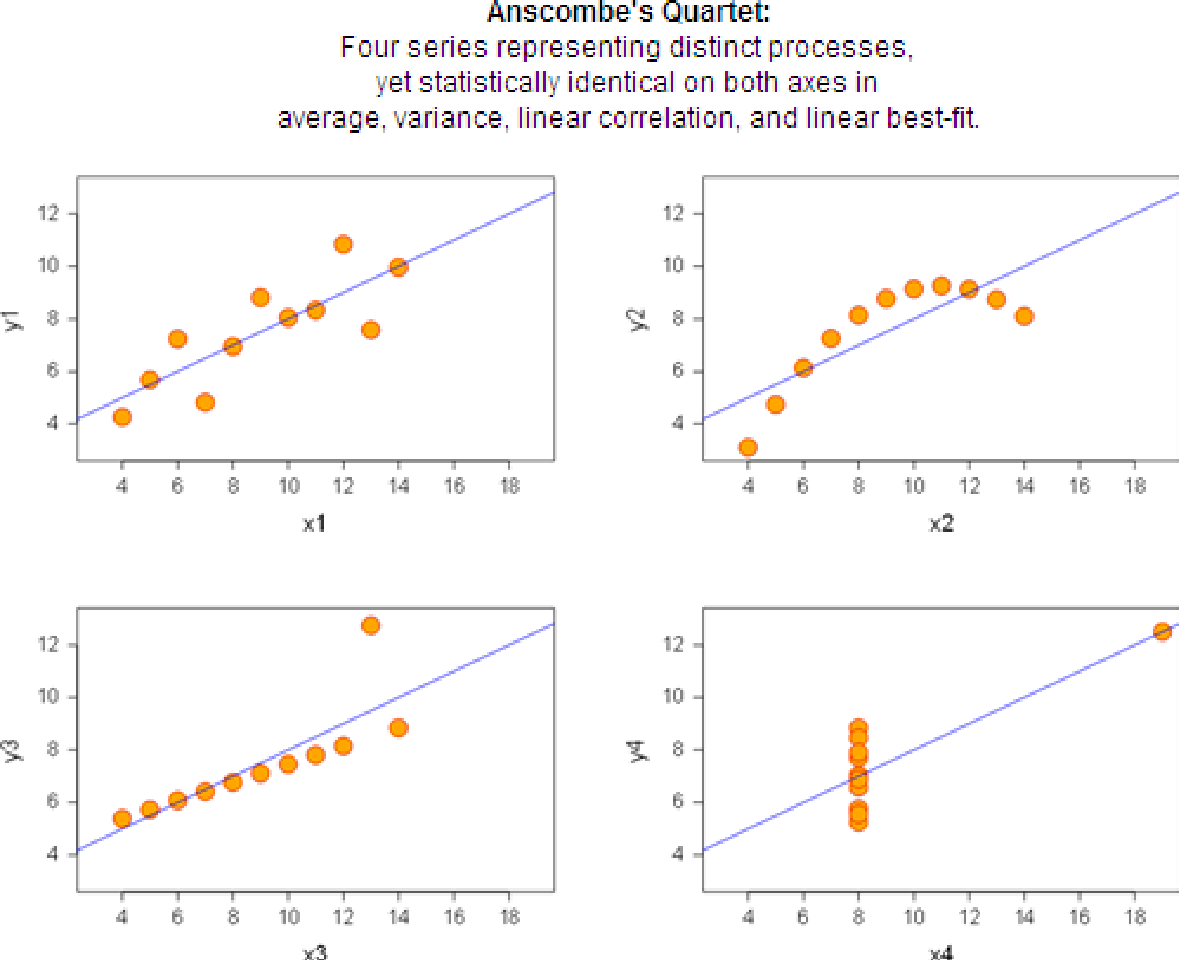
\includegraphics[width=300px]{col11306.imgs/m39404_anscombe.png} % m39404;anscombe.png;;;6.0;8.5;
      \vspace{2pt}
    \vspace{\rubberspace}\par \begin{cnxcaption}
	  \small \textbf{Figure 16.6: }Anscombe's quartet
	\end{cnxcaption}
    \vspace{.1in}
    \end{center}
 \end{figure}       \par 
\label{m39404*cid8}
%             \subsection{ Misuse of Statistics - For enrichment, not in CAPS}
            \nopagebreak
      \label{m39404*id215969}In many cases groups can gain an advantage by misleading people with the misuse of statistics. Companies misuse statistics to attempt to show that they are performing better than a competitor, advertisers abuse statistics to try to convince you to buy their product, researchers misuse statistics to attempt to show that their data is of better quality than it really is, etc.\par 
      \label{m39404*id215973}Common techniques used include:\par 
      \label{m39404*id215979}\begin{itemize}[noitemsep]
            \label{m39404*uid105}\item Three dimensional graphs.
\label{m39404*uid106}\item Axes that do not start at zero.
\label{m39404*uid107}\item Axes without scales.
\label{m39404*uid108}\item Graphic images that convey a negative or positive mood.
\label{m39404*uid109}\item Assumption that a correlation shows a necessary causality.
\label{m39404*uid110}\item Using statistics that are not truly representative of the entire population.
\label{m39404*uid111}\item Using misconceptions of mathematical concepts
\end{itemize}
      \label{m39404*id216070}For example, the following pairs of graphs show identical information but look very different. Explain why.\par 
      \label{m39404*id216074}
    \setcounter{subfigure}{0}
	\begin{figure}[H] % horizontal\label{m39404*id216077}
    \begin{center}
    \label{m39404*id216077!!!underscore!!!media}\label{m39404*id216077!!!underscore!!!printimage}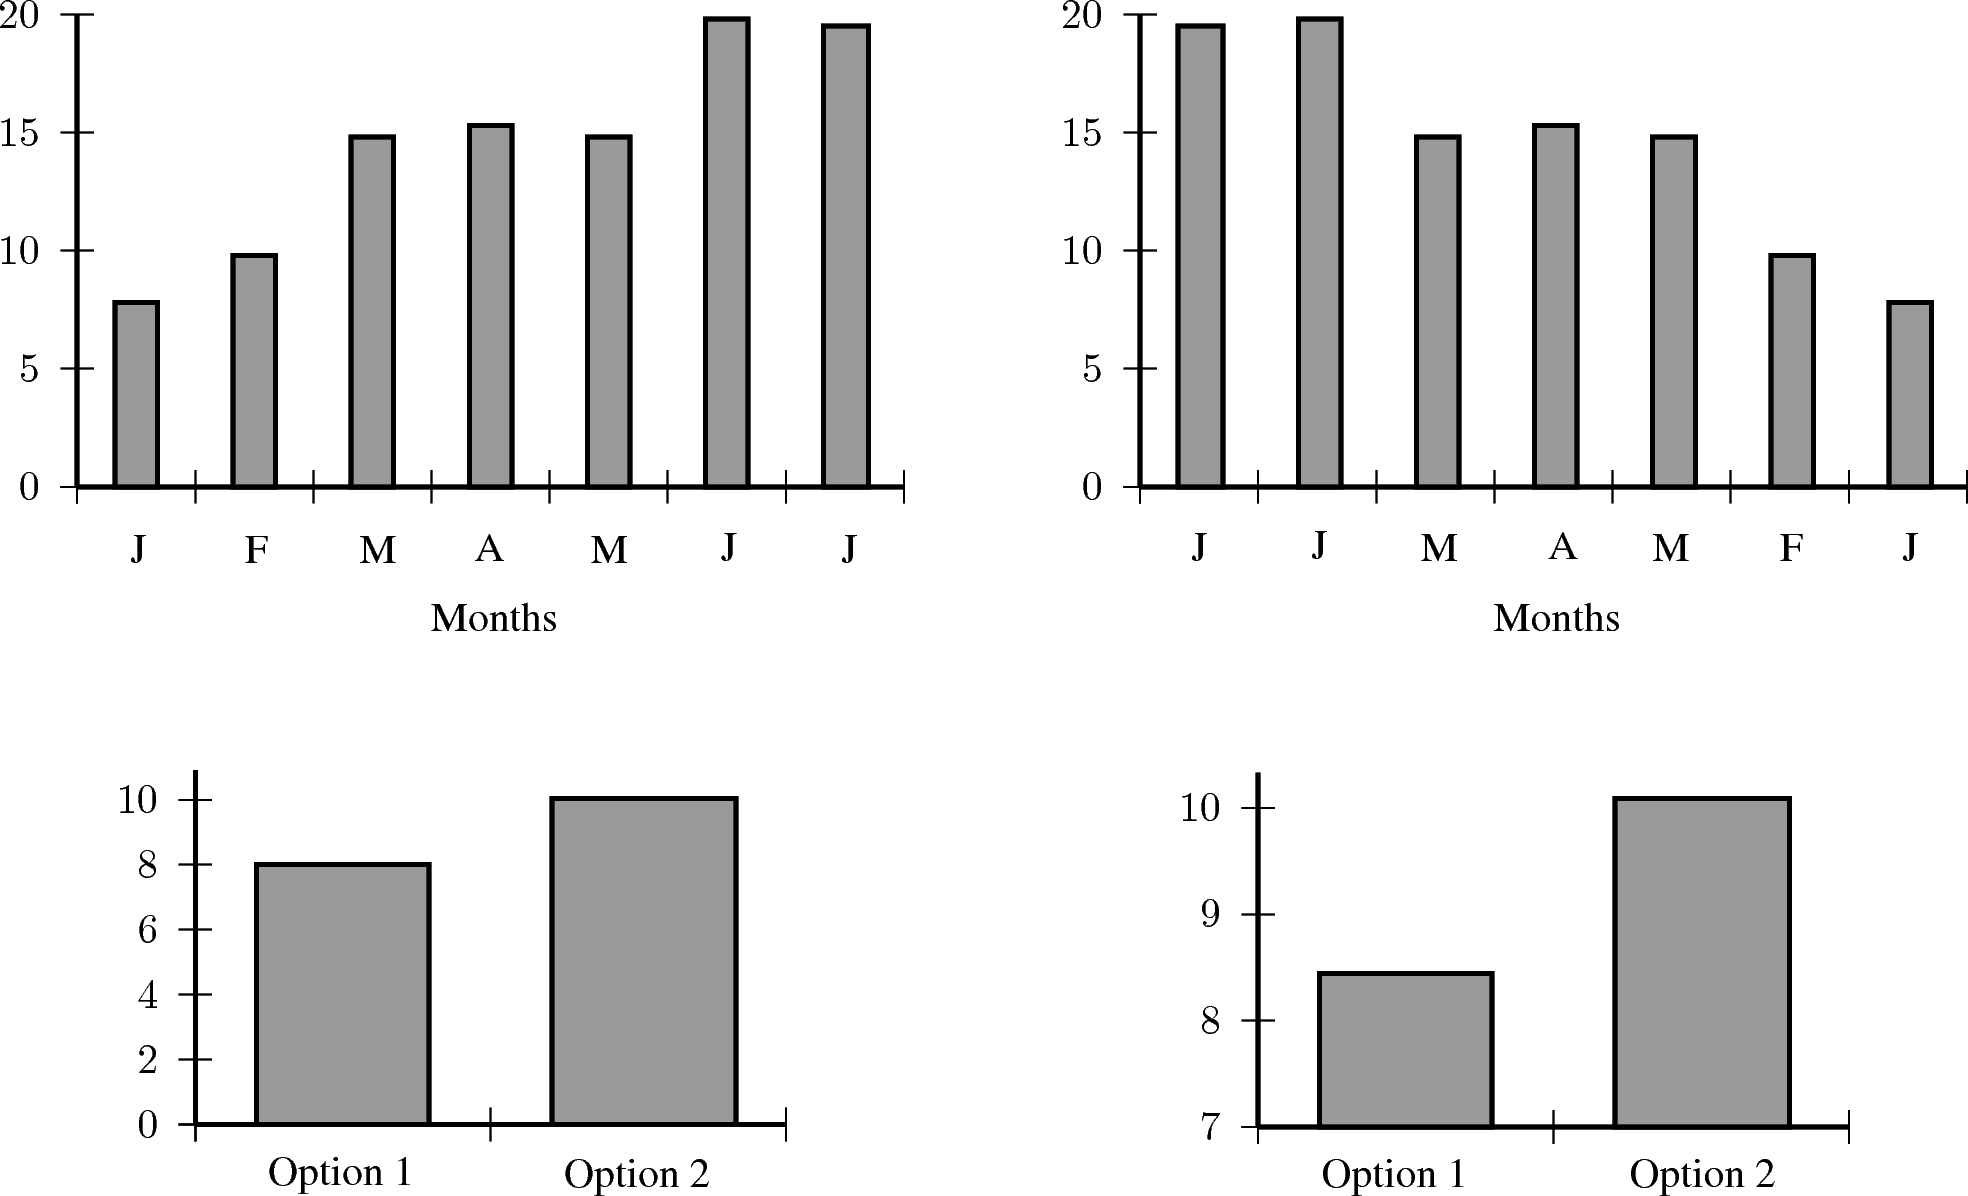
\includegraphics{col11306.imgs/m39404_MG10C16_010.png} % m39404;MG10C16\_010.png;;;6.0;8.5;
      \vspace{2pt}
    \vspace{.1in}
    \end{center}
 \end{figure}       
      \par 
      \label{m39404*uid112}
            \subsubsection{ Exercises - Application of Statistics}
            \nopagebreak
        \label{m39404*id216093}\begin{enumerate}[noitemsep, label=\textbf{\arabic*}. ] 
            \label{m39404*uid113}\item A company has tried to give a visual representation of the increase in their earnings from one year to the next. Does the graph below convince you? Critically analyse the graph.
    \setcounter{subfigure}{0}
	\begin{figure}[H] % horizontal\label{m39404*id216113}
    \begin{center}
    \label{m39404*id216113!!!underscore!!!media}\label{m39404*id216113!!!underscore!!!printimage}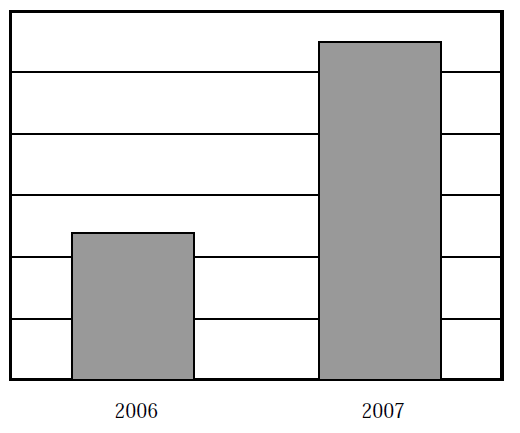
\includegraphics[width=300px]{col11306.imgs/m39404_MG10C16_011.png} % m39404;MG10C16\_011.png;;;6.0;8.5;
      \vspace{2pt}
    \vspace{.1in}
    \end{center}
 \end{figure}               \label{m39404*uid114}\item In a study conducted on a busy highway, data was collected about drivers breaking the speed limit and the colour of the car they were driving. The data were collected during a 20 minute time interval during the middle of the day, and are presented in a table and pie chart below.
\label{m39404*id216251}\begin{itemize}[noitemsep]
            \label{m39404*uid115}\item Conclusions made by a novice based on the data are summarised as follows:
\label{m39404*uid116}\item ``People driving white cars are more likely to break the speed limit.''
\label{m39404*uid117}\item ``Drivers in blue and red cars are more likely to stick to the speed limit.''
\label{m39404*uid118}\item Do you agree with these conclusions? Explain.
\end{itemize}
                \label{m39404*uid119}\item A record label produces a graphic, showing their advantage in sales over their competitors. Identify at least three devices they have used to influence and mislead the readers impression.
    \setcounter{subfigure}{0}
	\begin{figure}[H] % horizontal\label{m39404*id216327}
    \begin{center}
    \label{m39404*id216327!!!underscore!!!media}\label{m39404*id216327!!!underscore!!!printimage}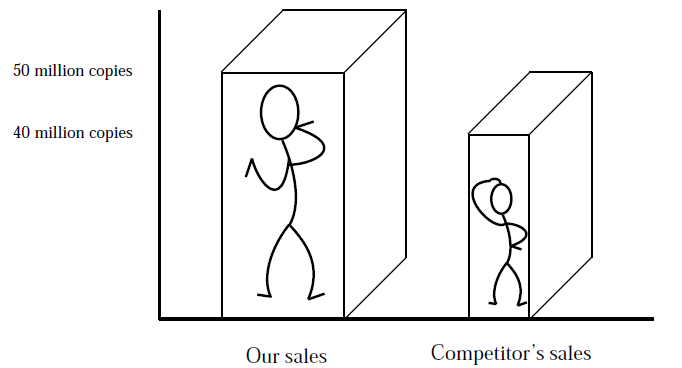
\includegraphics[width=300px]{col11306.imgs/m39404_MG10C16_013.png} % m39404;MG10C16\_013.png;;;6.0;8.5;
      \vspace{2pt}
    \vspace{.1in}
    \end{center}
 \end{figure}               \label{m39404*uid120}\item In an effort to discredit their competition, a tour bus company prints the graph shown below. Their claim is that the competitor is losing business. Can you think of a better explanation?
    \setcounter{subfigure}{0}
	\begin{figure}[H] % horizontal\label{m39404*id216351}
    \begin{center}
    \label{m39404*id216351!!!underscore!!!media}\label{m39404*id216351!!!underscore!!!printimage}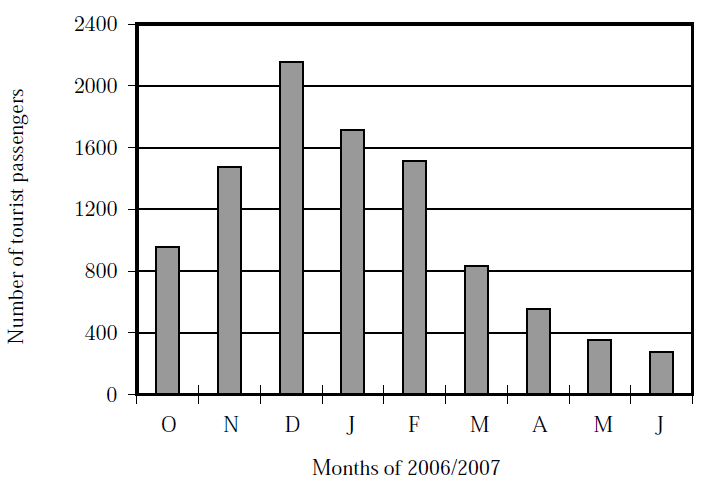
\includegraphics[width=300px]{col11306.imgs/m39404_MG10C16_014.png} % m39404;MG10C16\_014.png;;;6.0;8.5;
      \vspace{2pt}
    \vspace{.1in}
    \end{center}
 \end{figure}               \label{m39404*uid121}\item To test a theory, 8 different offices were monitored for noise levels and productivity of the employees in the office. The results are graphed below.
    \setcounter{subfigure}{0}
	\begin{figure}[H] % horizontal\label{m39404*id216374}
    \begin{center}
    \label{m39404*id216374!!!underscore!!!media}\label{m39404*id216374!!!underscore!!!printimage}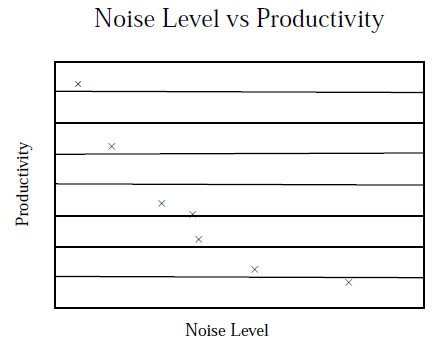
\includegraphics[width=300px]{col11306.imgs/m39404_MG10C16_015.png} % m39404;MG10C16\_015.png;;;6.0;8.5;
      \vspace{2pt}
    \vspace{.1in}
    \end{center}
 \end{figure}       
The following statement was then made:
``If an office environment is noisy, this leads to poor productivity.''
Explain the flaws in this thinking.\newline
\end{enumerate}
\label{m39404*cid9}
\par \raisebox{-5 pt}{
\includegraphics[width=0.5cm]{col11306.imgs/summary_www.png}} Find the answers with the shortcodes:
 \par \begin{tabular}[h]{cccccc}
 (1.) l4R  &  (2.) l4n  &  (3.) l4Q  &  (4.) l4U  &  (5.) l4P  & \end{tabular}
            \subsection{ End of chapter summary}
            \nopagebreak
            \label{m39404*id216407}\begin{itemize}[noitemsep, label=\textbullet{}]
            \item Data types can be divided into primary and secondary data. Primary data may be further divided into qualitative and quantitative data.\label{m39404*id97322}\item We use the following as measures of central tendency:\label{m39404*id67453}\begin{itemize}[noitemsep]
            \label{m39404*uid122}\item The mean of a data set, \begin{math}x\end{math}, denoted by \begin{math}\overline{x}\end{math}, is the average of the data values, and is calculated as:
\label{m39404*id216451}\nopagebreak\noindent{}\settowidth{\mymathboxwidth}{\begin{equation}
    \overline{x}=\frac{\mathrm{sum\; of\; values}}{\mathrm{number\; of\; values}}\tag{16.7}
      \end{equation}
    }
    \typeout{Columnwidth = \the\columnwidth}\typeout{math as usual width = \the\mymathboxwidth}
    \ifthenelse{\lengthtest{\mymathboxwidth < \columnwidth}}{% if the math fits, do it again, for real
    \begin{equation}
    \overline{x}=\frac{\mathrm{sum\; of\; values}}{\mathrm{number\; of\; values}}\tag{16.7}
      \end{equation}
    }{% else, if it doesn't fit
    \setlength{\mymathboxwidth}{\columnwidth}
      \addtolength{\mymathboxwidth}{-48pt}
    \par\vspace{12pt}\noindent\begin{minipage}{\columnwidth}
    \parbox[t]{\mymathboxwidth}{\large\begin{math}
    \overline{x}=\frac{\mathrm{sum\; of\; values}}{\mathrm{number\; of\; values}}\end{math}}\hfill
    \parbox[t]{48pt}{\raggedleft 
    (16.7)}
    \end{minipage}\vspace{12pt}\par
    }% end of conditional for this bit of math
    \typeout{math as usual width = \the\mymathboxwidth}
    \label{m39404*uid123}\item The median is the centre data value in a data set that has been ordered from lowest to highest
\label{m39404*uid12454}\item The mode is the data value that occurs most often in a data set.
\end{itemize}
        \label{m39404*id973243222}\item The following are measures of dispersion:\label{m39404*id6743453453}\begin{itemize}[noitemsep]
            \label{m39404*uid12542}\item The range of a data set is the difference between the lowest value and the highest value in the set. \label{m39404*uid123543}\item Quartiles are the three data values that divide an ordered data set into four groups containing equal numbers of data values. The median is the second quartile. 
\label{m39404*uid124}\item Percentiles are the 99 data values that divide a data set into 100 groups. 
\label{m39404*uid124342}\item The inter quartile range is a measure which provides information about the spread of a data set, and is calculated by subtracting the first quartile from the third quartile, giving the range of the middle half of the data set, trimming off the lowest and highest quarters, i.e. \begin{math}{Q}_{3}-{Q}_{1}\end{math}. Half of this value is the semi-interquartile range.\end{itemize}
        \item The five number summary is a way to summarise data. A box and whisker plot is a graphical representation of the five number summary.\item Random errors are found in all sets of data and arise from estimating data values. Bias or systematic error occurs when you consistently under or over estimate data values.\item You must always consider the data and the statistics that summarise the data\end{itemize}
    \label{m39404*cid10}
            \subsection{ End of Chapter Exercises}
            \nopagebreak
      \label{m39404*id216570}\begin{enumerate}[noitemsep, label=\textbf{\arabic*}. ] 
            \label{m39404*uid125}\item Calculate the mean, median, and mode of Data Set 3.\newline
\label{m39404*uid126}\item The tallest 7 trees in a park have heights in metres of 41, 60, 47, 42, 44, 42, and 47. Find the median of their heights.\newline
\label{m39404*uid127}\item The students in Bjorn's class have the following ages: 5, 6, 7, 5, 4, 6, 6, 6, 7, 4. Find the mode of their ages.\newline
\label{m39404*uid132}\item An engineering company has designed two different types of engines for motorbikes. The two different motorbikes are tested for the time it takes (in seconds) for them to accelerate from 0 km/h to 60 km/h.
    % \textbf{m39404*id217268}\par
    % how many colspecs?  12
          % name: cnx:colspec
            % colnum: 1
            % colwidth: 10*
            % latex-name: columna
            % colname: 
            % align/tgroup-align/default: //left
            % -------------------------
            % name: cnx:colspec
            % colnum: 2
            % colwidth: 10*
            % latex-name: columnb
            % colname: 
            % align/tgroup-align/default: //left
            % -------------------------
            % name: cnx:colspec
            % colnum: 3
            % colwidth: 10*
            % latex-name: columnc
            % colname: 
            % align/tgroup-align/default: //left
            % -------------------------
            % name: cnx:colspec
            % colnum: 4
            % colwidth: 10*
            % latex-name: columnd
            % colname: 
            % align/tgroup-align/default: //left
            % -------------------------
            % name: cnx:colspec
            % colnum: 5
            % colwidth: 10*
            % latex-name: columne
            % colname: 
            % align/tgroup-align/default: //left
            % -------------------------
            % name: cnx:colspec
            % colnum: 6
            % colwidth: 10*
            % latex-name: columnf
            % colname: 
            % align/tgroup-align/default: //left
            % -------------------------
            % name: cnx:colspec
            % colnum: 7
            % colwidth: 10*
            % latex-name: columng
            % colname: 
            % align/tgroup-align/default: //left
            % -------------------------
            % name: cnx:colspec
            % colnum: 8
            % colwidth: 10*
            % latex-name: columnh
            % colname: 
            % align/tgroup-align/default: //left
            % -------------------------
            % name: cnx:colspec
            % colnum: 9
            % colwidth: 10*
            % latex-name: columni
            % colname: 
            % align/tgroup-align/default: //left
            % -------------------------
            % name: cnx:colspec
            % colnum: 10
            % colwidth: 10*
            % latex-name: columnj
            % colname: 
            % align/tgroup-align/default: //left
            % -------------------------
            % name: cnx:colspec
            % colnum: 11
            % colwidth: 10*
            % latex-name: columnk
            % colname: 
            % align/tgroup-align/default: //left
            % -------------------------
            % name: cnx:colspec
            % colnum: 12
            % colwidth: 10*
            % latex-name: columnl
            % colname: 
            % align/tgroup-align/default: //left
            % -------------------------
    \setlength\mytablespace{24\tabcolsep}
    \addtolength\mytablespace{13\arrayrulewidth}
    \setlength\mytablewidth{\linewidth}
    \setlength\mytableroom{\mytablewidth}
    \addtolength\mytableroom{-\mytablespace}
    \setlength\myfixedwidth{0pt}
    \setlength\mystarwidth{\mytableroom}
        \addtolength\mystarwidth{-\myfixedwidth}
        \divide\mystarwidth 120
      % ----- Begin capturing width of table in LR mode woof
      \settowidth{\mytableboxwidth}{\begin{tabular}[t]{|l|l|l|l|l|l|l|l|l|l|l|l|}\hline
    % count in rowspan-info-nodeset: 12
    % align/colidx: left,1
    % rowcount: '0' | start: 'false' | colidx: '1'
        % Formatting a regular cell and recurring on the next sibling
         &
      % align/colidx: left,2
    % rowcount: '0' | start: 'false' | colidx: '2'
        % Formatting a regular cell and recurring on the next sibling
        Test 1 &
      % align/colidx: left,3
    % rowcount: '0' | start: 'false' | colidx: '3'
        % Formatting a regular cell and recurring on the next sibling
        Test 2 &
      % align/colidx: left,4
    % rowcount: '0' | start: 'false' | colidx: '4'
        % Formatting a regular cell and recurring on the next sibling
        Test 3 &
      % align/colidx: left,5
    % rowcount: '0' | start: 'false' | colidx: '5'
        % Formatting a regular cell and recurring on the next sibling
        Test 4 &
      % align/colidx: left,6
    % rowcount: '0' | start: 'false' | colidx: '6'
        % Formatting a regular cell and recurring on the next sibling
        Test 5 &
      % align/colidx: left,7
    % rowcount: '0' | start: 'false' | colidx: '7'
        % Formatting a regular cell and recurring on the next sibling
        Test 6 &
      % align/colidx: left,8
    % rowcount: '0' | start: 'false' | colidx: '8'
        % Formatting a regular cell and recurring on the next sibling
        Test 7 &
      % align/colidx: left,9
    % rowcount: '0' | start: 'false' | colidx: '9'
        % Formatting a regular cell and recurring on the next sibling
        Test 8 &
      % align/colidx: left,10
    % rowcount: '0' | start: 'false' | colidx: '10'
        % Formatting a regular cell and recurring on the next sibling
        Test 9 &
      % align/colidx: left,11
    % rowcount: '0' | start: 'false' | colidx: '11'
        % Formatting a regular cell and recurring on the next sibling
        Test 10 &
      % align/colidx: left,12
    % rowcount: '0' | start: 'false' | colidx: '12'
        % Formatting a regular cell and recurring on the next sibling
        Average% make-rowspan-placeholders
    % rowspan info: col1 '0' | 'false' | '' || col2 '0' | 'false' | '' || col3 '0' | 'false' | '' || col4 '0' | 'false' | '' || col5 '0' | 'false' | '' || col6 '0' | 'false' | '' || col7 '0' | 'false' | '' || col8 '0' | 'false' | '' || col9 '0' | 'false' | '' || col10 '0' | 'false' | '' || col11 '0' | 'false' | '' || col12 '0' | 'false' | ''
     \tabularnewline\cline{1-1}\cline{2-2}\cline{3-3}\cline{4-4}\cline{5-5}\cline{6-6}\cline{7-7}\cline{8-8}\cline{9-9}\cline{10-10}\cline{11-11}\cline{12-12}
      %--------------------------------------------------------------------
    % align/colidx: left,1
    % rowcount: '0' | start: 'false' | colidx: '1'
        % Formatting a regular cell and recurring on the next sibling
        Bike 1 &
      % align/colidx: left,2
    % rowcount: '0' | start: 'false' | colidx: '2'
        % Formatting a regular cell and recurring on the next sibling
        1.55 &
      % align/colidx: left,3
    % rowcount: '0' | start: 'false' | colidx: '3'
        % Formatting a regular cell and recurring on the next sibling
        1.00 &
      % align/colidx: left,4
    % rowcount: '0' | start: 'false' | colidx: '4'
        % Formatting a regular cell and recurring on the next sibling
        0.92 &
      % align/colidx: left,5
    % rowcount: '0' | start: 'false' | colidx: '5'
        % Formatting a regular cell and recurring on the next sibling
        0.80 &
      % align/colidx: left,6
    % rowcount: '0' | start: 'false' | colidx: '6'
        % Formatting a regular cell and recurring on the next sibling
        1.49 &
      % align/colidx: left,7
    % rowcount: '0' | start: 'false' | colidx: '7'
        % Formatting a regular cell and recurring on the next sibling
        0.71 &
      % align/colidx: left,8
    % rowcount: '0' | start: 'false' | colidx: '8'
        % Formatting a regular cell and recurring on the next sibling
        1.06 &
      % align/colidx: left,9
    % rowcount: '0' | start: 'false' | colidx: '9'
        % Formatting a regular cell and recurring on the next sibling
        0.68 &
      % align/colidx: left,10
    % rowcount: '0' | start: 'false' | colidx: '10'
        % Formatting a regular cell and recurring on the next sibling
        0.87 &
      % align/colidx: left,11
    % rowcount: '0' | start: 'false' | colidx: '11'
        % Formatting a regular cell and recurring on the next sibling
        1.09 &
      % align/colidx: left,12
    % rowcount: '0' | start: 'false' | colidx: '12'
        % Formatting a regular cell and recurring on the next sibling
        % make-rowspan-placeholders
    % rowspan info: col1 '0' | 'false' | '' || col2 '0' | 'false' | '' || col3 '0' | 'false' | '' || col4 '0' | 'false' | '' || col5 '0' | 'false' | '' || col6 '0' | 'false' | '' || col7 '0' | 'false' | '' || col8 '0' | 'false' | '' || col9 '0' | 'false' | '' || col10 '0' | 'false' | '' || col11 '0' | 'false' | '' || col12 '0' | 'false' | ''
     \tabularnewline\cline{1-1}\cline{2-2}\cline{3-3}\cline{4-4}\cline{5-5}\cline{6-6}\cline{7-7}\cline{8-8}\cline{9-9}\cline{10-10}\cline{11-11}\cline{12-12}
      %--------------------------------------------------------------------
    % align/colidx: left,1
    % rowcount: '0' | start: 'false' | colidx: '1'
        % Formatting a regular cell and recurring on the next sibling
        Bike 2 &
      % align/colidx: left,2
    % rowcount: '0' | start: 'false' | colidx: '2'
        % Formatting a regular cell and recurring on the next sibling
        0.9 &
      % align/colidx: left,3
    % rowcount: '0' | start: 'false' | colidx: '3'
        % Formatting a regular cell and recurring on the next sibling
        1.0 &
      % align/colidx: left,4
    % rowcount: '0' | start: 'false' | colidx: '4'
        % Formatting a regular cell and recurring on the next sibling
        1.1 &
      % align/colidx: left,5
    % rowcount: '0' | start: 'false' | colidx: '5'
        % Formatting a regular cell and recurring on the next sibling
        1.0 &
      % align/colidx: left,6
    % rowcount: '0' | start: 'false' | colidx: '6'
        % Formatting a regular cell and recurring on the next sibling
        1.0 &
      % align/colidx: left,7
    % rowcount: '0' | start: 'false' | colidx: '7'
        % Formatting a regular cell and recurring on the next sibling
        0.9 &
      % align/colidx: left,8
    % rowcount: '0' | start: 'false' | colidx: '8'
        % Formatting a regular cell and recurring on the next sibling
        0.9 &
      % align/colidx: left,9
    % rowcount: '0' | start: 'false' | colidx: '9'
        % Formatting a regular cell and recurring on the next sibling
        1.0 &
      % align/colidx: left,10
    % rowcount: '0' | start: 'false' | colidx: '10'
        % Formatting a regular cell and recurring on the next sibling
        0.9 &
      % align/colidx: left,11
    % rowcount: '0' | start: 'false' | colidx: '11'
        % Formatting a regular cell and recurring on the next sibling
        1.1 &
      % align/colidx: left,12
    % rowcount: '0' | start: 'false' | colidx: '12'
        % Formatting a regular cell and recurring on the next sibling
        % make-rowspan-placeholders
    % rowspan info: col1 '0' | 'false' | '' || col2 '0' | 'false' | '' || col3 '0' | 'false' | '' || col4 '0' | 'false' | '' || col5 '0' | 'false' | '' || col6 '0' | 'false' | '' || col7 '0' | 'false' | '' || col8 '0' | 'false' | '' || col9 '0' | 'false' | '' || col10 '0' | 'false' | '' || col11 '0' | 'false' | '' || col12 '0' | 'false' | ''
     \tabularnewline\cline{1-1}\cline{2-2}\cline{3-3}\cline{4-4}\cline{5-5}\cline{6-6}\cline{7-7}\cline{8-8}\cline{9-9}\cline{10-10}\cline{11-11}\cline{12-12}
      %--------------------------------------------------------------------
    \end{tabular}} % end mytableboxwidth set      
      % ----- End capturing width of table in LR mode
        % ----- LR or paragraph mode: must test
        % ----- Begin capturing height of table
        \settoheight{\mytableboxheight}{\begin{tabular}[t]{|l|l|l|l|l|l|l|l|l|l|l|l|}\hline
    % count in rowspan-info-nodeset: 12
    % align/colidx: left,1
    % rowcount: '0' | start: 'false' | colidx: '1'
        % Formatting a regular cell and recurring on the next sibling
         &
      % align/colidx: left,2
    % rowcount: '0' | start: 'false' | colidx: '2'
        % Formatting a regular cell and recurring on the next sibling
        Test 1 &
      % align/colidx: left,3
    % rowcount: '0' | start: 'false' | colidx: '3'
        % Formatting a regular cell and recurring on the next sibling
        Test 2 &
      % align/colidx: left,4
    % rowcount: '0' | start: 'false' | colidx: '4'
        % Formatting a regular cell and recurring on the next sibling
        Test 3 &
      % align/colidx: left,5
    % rowcount: '0' | start: 'false' | colidx: '5'
        % Formatting a regular cell and recurring on the next sibling
        Test 4 &
      % align/colidx: left,6
    % rowcount: '0' | start: 'false' | colidx: '6'
        % Formatting a regular cell and recurring on the next sibling
        Test 5 &
      % align/colidx: left,7
    % rowcount: '0' | start: 'false' | colidx: '7'
        % Formatting a regular cell and recurring on the next sibling
        Test 6 &
      % align/colidx: left,8
    % rowcount: '0' | start: 'false' | colidx: '8'
        % Formatting a regular cell and recurring on the next sibling
        Test 7 &
      % align/colidx: left,9
    % rowcount: '0' | start: 'false' | colidx: '9'
        % Formatting a regular cell and recurring on the next sibling
        Test 8 &
      % align/colidx: left,10
    % rowcount: '0' | start: 'false' | colidx: '10'
        % Formatting a regular cell and recurring on the next sibling
        Test 9 &
      % align/colidx: left,11
    % rowcount: '0' | start: 'false' | colidx: '11'
        % Formatting a regular cell and recurring on the next sibling
        Test 10 &
      % align/colidx: left,12
    % rowcount: '0' | start: 'false' | colidx: '12'
        % Formatting a regular cell and recurring on the next sibling
        Average% make-rowspan-placeholders
    % rowspan info: col1 '0' | 'false' | '' || col2 '0' | 'false' | '' || col3 '0' | 'false' | '' || col4 '0' | 'false' | '' || col5 '0' | 'false' | '' || col6 '0' | 'false' | '' || col7 '0' | 'false' | '' || col8 '0' | 'false' | '' || col9 '0' | 'false' | '' || col10 '0' | 'false' | '' || col11 '0' | 'false' | '' || col12 '0' | 'false' | ''
     \tabularnewline\cline{1-1}\cline{2-2}\cline{3-3}\cline{4-4}\cline{5-5}\cline{6-6}\cline{7-7}\cline{8-8}\cline{9-9}\cline{10-10}\cline{11-11}\cline{12-12}
      %--------------------------------------------------------------------
    % align/colidx: left,1
    % rowcount: '0' | start: 'false' | colidx: '1'
        % Formatting a regular cell and recurring on the next sibling
        Bike 1 &
      % align/colidx: left,2
    % rowcount: '0' | start: 'false' | colidx: '2'
        % Formatting a regular cell and recurring on the next sibling
        1.55 &
      % align/colidx: left,3
    % rowcount: '0' | start: 'false' | colidx: '3'
        % Formatting a regular cell and recurring on the next sibling
        1.00 &
      % align/colidx: left,4
    % rowcount: '0' | start: 'false' | colidx: '4'
        % Formatting a regular cell and recurring on the next sibling
        0.92 &
      % align/colidx: left,5
    % rowcount: '0' | start: 'false' | colidx: '5'
        % Formatting a regular cell and recurring on the next sibling
        0.80 &
      % align/colidx: left,6
    % rowcount: '0' | start: 'false' | colidx: '6'
        % Formatting a regular cell and recurring on the next sibling
        1.49 &
      % align/colidx: left,7
    % rowcount: '0' | start: 'false' | colidx: '7'
        % Formatting a regular cell and recurring on the next sibling
        0.71 &
      % align/colidx: left,8
    % rowcount: '0' | start: 'false' | colidx: '8'
        % Formatting a regular cell and recurring on the next sibling
        1.06 &
      % align/colidx: left,9
    % rowcount: '0' | start: 'false' | colidx: '9'
        % Formatting a regular cell and recurring on the next sibling
        0.68 &
      % align/colidx: left,10
    % rowcount: '0' | start: 'false' | colidx: '10'
        % Formatting a regular cell and recurring on the next sibling
        0.87 &
      % align/colidx: left,11
    % rowcount: '0' | start: 'false' | colidx: '11'
        % Formatting a regular cell and recurring on the next sibling
        1.09 &
      % align/colidx: left,12
    % rowcount: '0' | start: 'false' | colidx: '12'
        % Formatting a regular cell and recurring on the next sibling
        % make-rowspan-placeholders
    % rowspan info: col1 '0' | 'false' | '' || col2 '0' | 'false' | '' || col3 '0' | 'false' | '' || col4 '0' | 'false' | '' || col5 '0' | 'false' | '' || col6 '0' | 'false' | '' || col7 '0' | 'false' | '' || col8 '0' | 'false' | '' || col9 '0' | 'false' | '' || col10 '0' | 'false' | '' || col11 '0' | 'false' | '' || col12 '0' | 'false' | ''
     \tabularnewline\cline{1-1}\cline{2-2}\cline{3-3}\cline{4-4}\cline{5-5}\cline{6-6}\cline{7-7}\cline{8-8}\cline{9-9}\cline{10-10}\cline{11-11}\cline{12-12}
      %--------------------------------------------------------------------
    % align/colidx: left,1
    % rowcount: '0' | start: 'false' | colidx: '1'
        % Formatting a regular cell and recurring on the next sibling
        Bike 2 &
      % align/colidx: left,2
    % rowcount: '0' | start: 'false' | colidx: '2'
        % Formatting a regular cell and recurring on the next sibling
        0.9 &
      % align/colidx: left,3
    % rowcount: '0' | start: 'false' | colidx: '3'
        % Formatting a regular cell and recurring on the next sibling
        1.0 &
      % align/colidx: left,4
    % rowcount: '0' | start: 'false' | colidx: '4'
        % Formatting a regular cell and recurring on the next sibling
        1.1 &
      % align/colidx: left,5
    % rowcount: '0' | start: 'false' | colidx: '5'
        % Formatting a regular cell and recurring on the next sibling
        1.0 &
      % align/colidx: left,6
    % rowcount: '0' | start: 'false' | colidx: '6'
        % Formatting a regular cell and recurring on the next sibling
        1.0 &
      % align/colidx: left,7
    % rowcount: '0' | start: 'false' | colidx: '7'
        % Formatting a regular cell and recurring on the next sibling
        0.9 &
      % align/colidx: left,8
    % rowcount: '0' | start: 'false' | colidx: '8'
        % Formatting a regular cell and recurring on the next sibling
        0.9 &
      % align/colidx: left,9
    % rowcount: '0' | start: 'false' | colidx: '9'
        % Formatting a regular cell and recurring on the next sibling
        1.0 &
      % align/colidx: left,10
    % rowcount: '0' | start: 'false' | colidx: '10'
        % Formatting a regular cell and recurring on the next sibling
        0.9 &
      % align/colidx: left,11
    % rowcount: '0' | start: 'false' | colidx: '11'
        % Formatting a regular cell and recurring on the next sibling
        1.1 &
      % align/colidx: left,12
    % rowcount: '0' | start: 'false' | colidx: '12'
        % Formatting a regular cell and recurring on the next sibling
        % make-rowspan-placeholders
    % rowspan info: col1 '0' | 'false' | '' || col2 '0' | 'false' | '' || col3 '0' | 'false' | '' || col4 '0' | 'false' | '' || col5 '0' | 'false' | '' || col6 '0' | 'false' | '' || col7 '0' | 'false' | '' || col8 '0' | 'false' | '' || col9 '0' | 'false' | '' || col10 '0' | 'false' | '' || col11 '0' | 'false' | '' || col12 '0' | 'false' | ''
     \tabularnewline\cline{1-1}\cline{2-2}\cline{3-3}\cline{4-4}\cline{5-5}\cline{6-6}\cline{7-7}\cline{8-8}\cline{9-9}\cline{10-10}\cline{11-11}\cline{12-12}
      %--------------------------------------------------------------------
    \end{tabular}} % end mytableboxheight set
        \settodepth{\mytableboxdepth}{\begin{tabular}[t]{|l|l|l|l|l|l|l|l|l|l|l|l|}\hline
    % count in rowspan-info-nodeset: 12
    % align/colidx: left,1
    % rowcount: '0' | start: 'false' | colidx: '1'
        % Formatting a regular cell and recurring on the next sibling
         &
      % align/colidx: left,2
    % rowcount: '0' | start: 'false' | colidx: '2'
        % Formatting a regular cell and recurring on the next sibling
        Test 1 &
      % align/colidx: left,3
    % rowcount: '0' | start: 'false' | colidx: '3'
        % Formatting a regular cell and recurring on the next sibling
        Test 2 &
      % align/colidx: left,4
    % rowcount: '0' | start: 'false' | colidx: '4'
        % Formatting a regular cell and recurring on the next sibling
        Test 3 &
      % align/colidx: left,5
    % rowcount: '0' | start: 'false' | colidx: '5'
        % Formatting a regular cell and recurring on the next sibling
        Test 4 &
      % align/colidx: left,6
    % rowcount: '0' | start: 'false' | colidx: '6'
        % Formatting a regular cell and recurring on the next sibling
        Test 5 &
      % align/colidx: left,7
    % rowcount: '0' | start: 'false' | colidx: '7'
        % Formatting a regular cell and recurring on the next sibling
        Test 6 &
      % align/colidx: left,8
    % rowcount: '0' | start: 'false' | colidx: '8'
        % Formatting a regular cell and recurring on the next sibling
        Test 7 &
      % align/colidx: left,9
    % rowcount: '0' | start: 'false' | colidx: '9'
        % Formatting a regular cell and recurring on the next sibling
        Test 8 &
      % align/colidx: left,10
    % rowcount: '0' | start: 'false' | colidx: '10'
        % Formatting a regular cell and recurring on the next sibling
        Test 9 &
      % align/colidx: left,11
    % rowcount: '0' | start: 'false' | colidx: '11'
        % Formatting a regular cell and recurring on the next sibling
        Test 10 &
      % align/colidx: left,12
    % rowcount: '0' | start: 'false' | colidx: '12'
        % Formatting a regular cell and recurring on the next sibling
        Average% make-rowspan-placeholders
    % rowspan info: col1 '0' | 'false' | '' || col2 '0' | 'false' | '' || col3 '0' | 'false' | '' || col4 '0' | 'false' | '' || col5 '0' | 'false' | '' || col6 '0' | 'false' | '' || col7 '0' | 'false' | '' || col8 '0' | 'false' | '' || col9 '0' | 'false' | '' || col10 '0' | 'false' | '' || col11 '0' | 'false' | '' || col12 '0' | 'false' | ''
     \tabularnewline\cline{1-1}\cline{2-2}\cline{3-3}\cline{4-4}\cline{5-5}\cline{6-6}\cline{7-7}\cline{8-8}\cline{9-9}\cline{10-10}\cline{11-11}\cline{12-12}
      %--------------------------------------------------------------------
    % align/colidx: left,1
    % rowcount: '0' | start: 'false' | colidx: '1'
        % Formatting a regular cell and recurring on the next sibling
        Bike 1 &
      % align/colidx: left,2
    % rowcount: '0' | start: 'false' | colidx: '2'
        % Formatting a regular cell and recurring on the next sibling
        1.55 &
      % align/colidx: left,3
    % rowcount: '0' | start: 'false' | colidx: '3'
        % Formatting a regular cell and recurring on the next sibling
        1.00 &
      % align/colidx: left,4
    % rowcount: '0' | start: 'false' | colidx: '4'
        % Formatting a regular cell and recurring on the next sibling
        0.92 &
      % align/colidx: left,5
    % rowcount: '0' | start: 'false' | colidx: '5'
        % Formatting a regular cell and recurring on the next sibling
        0.80 &
      % align/colidx: left,6
    % rowcount: '0' | start: 'false' | colidx: '6'
        % Formatting a regular cell and recurring on the next sibling
        1.49 &
      % align/colidx: left,7
    % rowcount: '0' | start: 'false' | colidx: '7'
        % Formatting a regular cell and recurring on the next sibling
        0.71 &
      % align/colidx: left,8
    % rowcount: '0' | start: 'false' | colidx: '8'
        % Formatting a regular cell and recurring on the next sibling
        1.06 &
      % align/colidx: left,9
    % rowcount: '0' | start: 'false' | colidx: '9'
        % Formatting a regular cell and recurring on the next sibling
        0.68 &
      % align/colidx: left,10
    % rowcount: '0' | start: 'false' | colidx: '10'
        % Formatting a regular cell and recurring on the next sibling
        0.87 &
      % align/colidx: left,11
    % rowcount: '0' | start: 'false' | colidx: '11'
        % Formatting a regular cell and recurring on the next sibling
        1.09 &
      % align/colidx: left,12
    % rowcount: '0' | start: 'false' | colidx: '12'
        % Formatting a regular cell and recurring on the next sibling
        % make-rowspan-placeholders
    % rowspan info: col1 '0' | 'false' | '' || col2 '0' | 'false' | '' || col3 '0' | 'false' | '' || col4 '0' | 'false' | '' || col5 '0' | 'false' | '' || col6 '0' | 'false' | '' || col7 '0' | 'false' | '' || col8 '0' | 'false' | '' || col9 '0' | 'false' | '' || col10 '0' | 'false' | '' || col11 '0' | 'false' | '' || col12 '0' | 'false' | ''
     \tabularnewline\cline{1-1}\cline{2-2}\cline{3-3}\cline{4-4}\cline{5-5}\cline{6-6}\cline{7-7}\cline{8-8}\cline{9-9}\cline{10-10}\cline{11-11}\cline{12-12}
      %--------------------------------------------------------------------
    % align/colidx: left,1
    % rowcount: '0' | start: 'false' | colidx: '1'
        % Formatting a regular cell and recurring on the next sibling
        Bike 2 &
      % align/colidx: left,2
    % rowcount: '0' | start: 'false' | colidx: '2'
        % Formatting a regular cell and recurring on the next sibling
        0.9 &
      % align/colidx: left,3
    % rowcount: '0' | start: 'false' | colidx: '3'
        % Formatting a regular cell and recurring on the next sibling
        1.0 &
      % align/colidx: left,4
    % rowcount: '0' | start: 'false' | colidx: '4'
        % Formatting a regular cell and recurring on the next sibling
        1.1 &
      % align/colidx: left,5
    % rowcount: '0' | start: 'false' | colidx: '5'
        % Formatting a regular cell and recurring on the next sibling
        1.0 &
      % align/colidx: left,6
    % rowcount: '0' | start: 'false' | colidx: '6'
        % Formatting a regular cell and recurring on the next sibling
        1.0 &
      % align/colidx: left,7
    % rowcount: '0' | start: 'false' | colidx: '7'
        % Formatting a regular cell and recurring on the next sibling
        0.9 &
      % align/colidx: left,8
    % rowcount: '0' | start: 'false' | colidx: '8'
        % Formatting a regular cell and recurring on the next sibling
        0.9 &
      % align/colidx: left,9
    % rowcount: '0' | start: 'false' | colidx: '9'
        % Formatting a regular cell and recurring on the next sibling
        1.0 &
      % align/colidx: left,10
    % rowcount: '0' | start: 'false' | colidx: '10'
        % Formatting a regular cell and recurring on the next sibling
        0.9 &
      % align/colidx: left,11
    % rowcount: '0' | start: 'false' | colidx: '11'
        % Formatting a regular cell and recurring on the next sibling
        1.1 &
      % align/colidx: left,12
    % rowcount: '0' | start: 'false' | colidx: '12'
        % Formatting a regular cell and recurring on the next sibling
        % make-rowspan-placeholders
    % rowspan info: col1 '0' | 'false' | '' || col2 '0' | 'false' | '' || col3 '0' | 'false' | '' || col4 '0' | 'false' | '' || col5 '0' | 'false' | '' || col6 '0' | 'false' | '' || col7 '0' | 'false' | '' || col8 '0' | 'false' | '' || col9 '0' | 'false' | '' || col10 '0' | 'false' | '' || col11 '0' | 'false' | '' || col12 '0' | 'false' | ''
     \tabularnewline\cline{1-1}\cline{2-2}\cline{3-3}\cline{4-4}\cline{5-5}\cline{6-6}\cline{7-7}\cline{8-8}\cline{9-9}\cline{10-10}\cline{11-11}\cline{12-12}
      %--------------------------------------------------------------------
    \end{tabular}} % end mytableboxdepth set
        \addtolength{\mytableboxheight}{\mytableboxdepth}
        % ----- End capturing height of table        
        \ifthenelse{\mytableboxwidth<\textwidth}{% the table fits in LR mode
          \addtolength{\mytableboxwidth}{-\mytablespace}
          \typeout{textheight: \the\textheight}
          \typeout{mytableboxheight: \the\mytableboxheight}
          \typeout{textwidth: \the\textwidth}
          \typeout{mytableboxwidth: \the\mytableboxwidth}
          \ifthenelse{\mytableboxheight<\textheight}{%
    % \begin{table}[H]
    % \\ 'id3001214' '1'
        \begin{center}
      \label{m39404*id217268}
    \noindent
    \begin{tabular}[t]{|l|l|l|l|l|l|l|l|l|l|l|l|}\hline
    % count in rowspan-info-nodeset: 12
    % align/colidx: left,1
    % rowcount: '0' | start: 'false' | colidx: '1'
        % Formatting a regular cell and recurring on the next sibling
         &
      % align/colidx: left,2
    % rowcount: '0' | start: 'false' | colidx: '2'
        % Formatting a regular cell and recurring on the next sibling
        Test 1 &
      % align/colidx: left,3
    % rowcount: '0' | start: 'false' | colidx: '3'
        % Formatting a regular cell and recurring on the next sibling
        Test 2 &
      % align/colidx: left,4
    % rowcount: '0' | start: 'false' | colidx: '4'
        % Formatting a regular cell and recurring on the next sibling
        Test 3 &
      % align/colidx: left,5
    % rowcount: '0' | start: 'false' | colidx: '5'
        % Formatting a regular cell and recurring on the next sibling
        Test 4 &
      % align/colidx: left,6
    % rowcount: '0' | start: 'false' | colidx: '6'
        % Formatting a regular cell and recurring on the next sibling
        Test 5 &
      % align/colidx: left,7
    % rowcount: '0' | start: 'false' | colidx: '7'
        % Formatting a regular cell and recurring on the next sibling
        Test 6 &
      % align/colidx: left,8
    % rowcount: '0' | start: 'false' | colidx: '8'
        % Formatting a regular cell and recurring on the next sibling
        Test 7 &
      % align/colidx: left,9
    % rowcount: '0' | start: 'false' | colidx: '9'
        % Formatting a regular cell and recurring on the next sibling
        Test 8 &
      % align/colidx: left,10
    % rowcount: '0' | start: 'false' | colidx: '10'
        % Formatting a regular cell and recurring on the next sibling
        Test 9 &
      % align/colidx: left,11
    % rowcount: '0' | start: 'false' | colidx: '11'
        % Formatting a regular cell and recurring on the next sibling
        Test 10 &
      % align/colidx: left,12
    % rowcount: '0' | start: 'false' | colidx: '12'
        % Formatting a regular cell and recurring on the next sibling
        Average% make-rowspan-placeholders
    % rowspan info: col1 '0' | 'false' | '' || col2 '0' | 'false' | '' || col3 '0' | 'false' | '' || col4 '0' | 'false' | '' || col5 '0' | 'false' | '' || col6 '0' | 'false' | '' || col7 '0' | 'false' | '' || col8 '0' | 'false' | '' || col9 '0' | 'false' | '' || col10 '0' | 'false' | '' || col11 '0' | 'false' | '' || col12 '0' | 'false' | ''
     \tabularnewline\cline{1-1}\cline{2-2}\cline{3-3}\cline{4-4}\cline{5-5}\cline{6-6}\cline{7-7}\cline{8-8}\cline{9-9}\cline{10-10}\cline{11-11}\cline{12-12}
      %--------------------------------------------------------------------
    % align/colidx: left,1
    % rowcount: '0' | start: 'false' | colidx: '1'
        % Formatting a regular cell and recurring on the next sibling
        Bike 1 &
      % align/colidx: left,2
    % rowcount: '0' | start: 'false' | colidx: '2'
        % Formatting a regular cell and recurring on the next sibling
        1.55 &
      % align/colidx: left,3
    % rowcount: '0' | start: 'false' | colidx: '3'
        % Formatting a regular cell and recurring on the next sibling
        1.00 &
      % align/colidx: left,4
    % rowcount: '0' | start: 'false' | colidx: '4'
        % Formatting a regular cell and recurring on the next sibling
        0.92 &
      % align/colidx: left,5
    % rowcount: '0' | start: 'false' | colidx: '5'
        % Formatting a regular cell and recurring on the next sibling
        0.80 &
      % align/colidx: left,6
    % rowcount: '0' | start: 'false' | colidx: '6'
        % Formatting a regular cell and recurring on the next sibling
        1.49 &
      % align/colidx: left,7
    % rowcount: '0' | start: 'false' | colidx: '7'
        % Formatting a regular cell and recurring on the next sibling
        0.71 &
      % align/colidx: left,8
    % rowcount: '0' | start: 'false' | colidx: '8'
        % Formatting a regular cell and recurring on the next sibling
        1.06 &
      % align/colidx: left,9
    % rowcount: '0' | start: 'false' | colidx: '9'
        % Formatting a regular cell and recurring on the next sibling
        0.68 &
      % align/colidx: left,10
    % rowcount: '0' | start: 'false' | colidx: '10'
        % Formatting a regular cell and recurring on the next sibling
        0.87 &
      % align/colidx: left,11
    % rowcount: '0' | start: 'false' | colidx: '11'
        % Formatting a regular cell and recurring on the next sibling
        1.09 &
      % align/colidx: left,12
    % rowcount: '0' | start: 'false' | colidx: '12'
        % Formatting a regular cell and recurring on the next sibling
        % make-rowspan-placeholders
    % rowspan info: col1 '0' | 'false' | '' || col2 '0' | 'false' | '' || col3 '0' | 'false' | '' || col4 '0' | 'false' | '' || col5 '0' | 'false' | '' || col6 '0' | 'false' | '' || col7 '0' | 'false' | '' || col8 '0' | 'false' | '' || col9 '0' | 'false' | '' || col10 '0' | 'false' | '' || col11 '0' | 'false' | '' || col12 '0' | 'false' | ''
     \tabularnewline\cline{1-1}\cline{2-2}\cline{3-3}\cline{4-4}\cline{5-5}\cline{6-6}\cline{7-7}\cline{8-8}\cline{9-9}\cline{10-10}\cline{11-11}\cline{12-12}
      %--------------------------------------------------------------------
    % align/colidx: left,1
    % rowcount: '0' | start: 'false' | colidx: '1'
        % Formatting a regular cell and recurring on the next sibling
        Bike 2 &
      % align/colidx: left,2
    % rowcount: '0' | start: 'false' | colidx: '2'
        % Formatting a regular cell and recurring on the next sibling
        0.9 &
      % align/colidx: left,3
    % rowcount: '0' | start: 'false' | colidx: '3'
        % Formatting a regular cell and recurring on the next sibling
        1.0 &
      % align/colidx: left,4
    % rowcount: '0' | start: 'false' | colidx: '4'
        % Formatting a regular cell and recurring on the next sibling
        1.1 &
      % align/colidx: left,5
    % rowcount: '0' | start: 'false' | colidx: '5'
        % Formatting a regular cell and recurring on the next sibling
        1.0 &
      % align/colidx: left,6
    % rowcount: '0' | start: 'false' | colidx: '6'
        % Formatting a regular cell and recurring on the next sibling
        1.0 &
      % align/colidx: left,7
    % rowcount: '0' | start: 'false' | colidx: '7'
        % Formatting a regular cell and recurring on the next sibling
        0.9 &
      % align/colidx: left,8
    % rowcount: '0' | start: 'false' | colidx: '8'
        % Formatting a regular cell and recurring on the next sibling
        0.9 &
      % align/colidx: left,9
    % rowcount: '0' | start: 'false' | colidx: '9'
        % Formatting a regular cell and recurring on the next sibling
        1.0 &
      % align/colidx: left,10
    % rowcount: '0' | start: 'false' | colidx: '10'
        % Formatting a regular cell and recurring on the next sibling
        0.9 &
      % align/colidx: left,11
    % rowcount: '0' | start: 'false' | colidx: '11'
        % Formatting a regular cell and recurring on the next sibling
        1.1 &
      % align/colidx: left,12
    % rowcount: '0' | start: 'false' | colidx: '12'
        % Formatting a regular cell and recurring on the next sibling
        % make-rowspan-placeholders
    % rowspan info: col1 '0' | 'false' | '' || col2 '0' | 'false' | '' || col3 '0' | 'false' | '' || col4 '0' | 'false' | '' || col5 '0' | 'false' | '' || col6 '0' | 'false' | '' || col7 '0' | 'false' | '' || col8 '0' | 'false' | '' || col9 '0' | 'false' | '' || col10 '0' | 'false' | '' || col11 '0' | 'false' | '' || col12 '0' | 'false' | ''
     \tabularnewline\cline{1-1}\cline{2-2}\cline{3-3}\cline{4-4}\cline{5-5}\cline{6-6}\cline{7-7}\cline{8-8}\cline{9-9}\cline{10-10}\cline{11-11}\cline{12-12}
      %--------------------------------------------------------------------
    \end{tabular}
      \end{center}
    \begin{center}{\small\bfseries Table 16.18}\end{center}
    %\end{table}
          }{ % else
    % \begin{table}[H]
    % \\ 'id3001214' '1'
        \begin{center}
      \label{m39404*id217268}
    \noindent
    \tabletail{%
        \hline
        \multicolumn{12}{|p{\mytableboxwidth}|}{\raggedleft \small \sl continued on next page}\\
        \hline
      }
      \tablelasttail{}
      \begin{xtabular}[t]{|l|l|l|l|l|l|l|l|l|l|l|l|}\hline
    % count in rowspan-info-nodeset: 12
    % align/colidx: left,1
    % rowcount: '0' | start: 'false' | colidx: '1'
        % Formatting a regular cell and recurring on the next sibling
         &
      % align/colidx: left,2
    % rowcount: '0' | start: 'false' | colidx: '2'
        % Formatting a regular cell and recurring on the next sibling
        Test 1 &
      % align/colidx: left,3
    % rowcount: '0' | start: 'false' | colidx: '3'
        % Formatting a regular cell and recurring on the next sibling
        Test 2 &
      % align/colidx: left,4
    % rowcount: '0' | start: 'false' | colidx: '4'
        % Formatting a regular cell and recurring on the next sibling
        Test 3 &
      % align/colidx: left,5
    % rowcount: '0' | start: 'false' | colidx: '5'
        % Formatting a regular cell and recurring on the next sibling
        Test 4 &
      % align/colidx: left,6
    % rowcount: '0' | start: 'false' | colidx: '6'
        % Formatting a regular cell and recurring on the next sibling
        Test 5 &
      % align/colidx: left,7
    % rowcount: '0' | start: 'false' | colidx: '7'
        % Formatting a regular cell and recurring on the next sibling
        Test 6 &
      % align/colidx: left,8
    % rowcount: '0' | start: 'false' | colidx: '8'
        % Formatting a regular cell and recurring on the next sibling
        Test 7 &
      % align/colidx: left,9
    % rowcount: '0' | start: 'false' | colidx: '9'
        % Formatting a regular cell and recurring on the next sibling
        Test 8 &
      % align/colidx: left,10
    % rowcount: '0' | start: 'false' | colidx: '10'
        % Formatting a regular cell and recurring on the next sibling
        Test 9 &
      % align/colidx: left,11
    % rowcount: '0' | start: 'false' | colidx: '11'
        % Formatting a regular cell and recurring on the next sibling
        Test 10 &
      % align/colidx: left,12
    % rowcount: '0' | start: 'false' | colidx: '12'
        % Formatting a regular cell and recurring on the next sibling
        Average% make-rowspan-placeholders
    % rowspan info: col1 '0' | 'false' | '' || col2 '0' | 'false' | '' || col3 '0' | 'false' | '' || col4 '0' | 'false' | '' || col5 '0' | 'false' | '' || col6 '0' | 'false' | '' || col7 '0' | 'false' | '' || col8 '0' | 'false' | '' || col9 '0' | 'false' | '' || col10 '0' | 'false' | '' || col11 '0' | 'false' | '' || col12 '0' | 'false' | ''
     \tabularnewline\cline{1-1}\cline{2-2}\cline{3-3}\cline{4-4}\cline{5-5}\cline{6-6}\cline{7-7}\cline{8-8}\cline{9-9}\cline{10-10}\cline{11-11}\cline{12-12}
      %--------------------------------------------------------------------
    % align/colidx: left,1
    % rowcount: '0' | start: 'false' | colidx: '1'
        % Formatting a regular cell and recurring on the next sibling
        Bike 1 &
      % align/colidx: left,2
    % rowcount: '0' | start: 'false' | colidx: '2'
        % Formatting a regular cell and recurring on the next sibling
        1.55 &
      % align/colidx: left,3
    % rowcount: '0' | start: 'false' | colidx: '3'
        % Formatting a regular cell and recurring on the next sibling
        1.00 &
      % align/colidx: left,4
    % rowcount: '0' | start: 'false' | colidx: '4'
        % Formatting a regular cell and recurring on the next sibling
        0.92 &
      % align/colidx: left,5
    % rowcount: '0' | start: 'false' | colidx: '5'
        % Formatting a regular cell and recurring on the next sibling
        0.80 &
      % align/colidx: left,6
    % rowcount: '0' | start: 'false' | colidx: '6'
        % Formatting a regular cell and recurring on the next sibling
        1.49 &
      % align/colidx: left,7
    % rowcount: '0' | start: 'false' | colidx: '7'
        % Formatting a regular cell and recurring on the next sibling
        0.71 &
      % align/colidx: left,8
    % rowcount: '0' | start: 'false' | colidx: '8'
        % Formatting a regular cell and recurring on the next sibling
        1.06 &
      % align/colidx: left,9
    % rowcount: '0' | start: 'false' | colidx: '9'
        % Formatting a regular cell and recurring on the next sibling
        0.68 &
      % align/colidx: left,10
    % rowcount: '0' | start: 'false' | colidx: '10'
        % Formatting a regular cell and recurring on the next sibling
        0.87 &
      % align/colidx: left,11
    % rowcount: '0' | start: 'false' | colidx: '11'
        % Formatting a regular cell and recurring on the next sibling
        1.09 &
      % align/colidx: left,12
    % rowcount: '0' | start: 'false' | colidx: '12'
        % Formatting a regular cell and recurring on the next sibling
        % make-rowspan-placeholders
    % rowspan info: col1 '0' | 'false' | '' || col2 '0' | 'false' | '' || col3 '0' | 'false' | '' || col4 '0' | 'false' | '' || col5 '0' | 'false' | '' || col6 '0' | 'false' | '' || col7 '0' | 'false' | '' || col8 '0' | 'false' | '' || col9 '0' | 'false' | '' || col10 '0' | 'false' | '' || col11 '0' | 'false' | '' || col12 '0' | 'false' | ''
     \tabularnewline\cline{1-1}\cline{2-2}\cline{3-3}\cline{4-4}\cline{5-5}\cline{6-6}\cline{7-7}\cline{8-8}\cline{9-9}\cline{10-10}\cline{11-11}\cline{12-12}
      %--------------------------------------------------------------------
    % align/colidx: left,1
    % rowcount: '0' | start: 'false' | colidx: '1'
        % Formatting a regular cell and recurring on the next sibling
        Bike 2 &
      % align/colidx: left,2
    % rowcount: '0' | start: 'false' | colidx: '2'
        % Formatting a regular cell and recurring on the next sibling
        0.9 &
      % align/colidx: left,3
    % rowcount: '0' | start: 'false' | colidx: '3'
        % Formatting a regular cell and recurring on the next sibling
        1.0 &
      % align/colidx: left,4
    % rowcount: '0' | start: 'false' | colidx: '4'
        % Formatting a regular cell and recurring on the next sibling
        1.1 &
      % align/colidx: left,5
    % rowcount: '0' | start: 'false' | colidx: '5'
        % Formatting a regular cell and recurring on the next sibling
        1.0 &
      % align/colidx: left,6
    % rowcount: '0' | start: 'false' | colidx: '6'
        % Formatting a regular cell and recurring on the next sibling
        1.0 &
      % align/colidx: left,7
    % rowcount: '0' | start: 'false' | colidx: '7'
        % Formatting a regular cell and recurring on the next sibling
        0.9 &
      % align/colidx: left,8
    % rowcount: '0' | start: 'false' | colidx: '8'
        % Formatting a regular cell and recurring on the next sibling
        0.9 &
      % align/colidx: left,9
    % rowcount: '0' | start: 'false' | colidx: '9'
        % Formatting a regular cell and recurring on the next sibling
        1.0 &
      % align/colidx: left,10
    % rowcount: '0' | start: 'false' | colidx: '10'
        % Formatting a regular cell and recurring on the next sibling
        0.9 &
      % align/colidx: left,11
    % rowcount: '0' | start: 'false' | colidx: '11'
        % Formatting a regular cell and recurring on the next sibling
        1.1 &
      % align/colidx: left,12
    % rowcount: '0' | start: 'false' | colidx: '12'
        % Formatting a regular cell and recurring on the next sibling
        % make-rowspan-placeholders
    % rowspan info: col1 '0' | 'false' | '' || col2 '0' | 'false' | '' || col3 '0' | 'false' | '' || col4 '0' | 'false' | '' || col5 '0' | 'false' | '' || col6 '0' | 'false' | '' || col7 '0' | 'false' | '' || col8 '0' | 'false' | '' || col9 '0' | 'false' | '' || col10 '0' | 'false' | '' || col11 '0' | 'false' | '' || col12 '0' | 'false' | ''
     \tabularnewline\cline{1-1}\cline{2-2}\cline{3-3}\cline{4-4}\cline{5-5}\cline{6-6}\cline{7-7}\cline{8-8}\cline{9-9}\cline{10-10}\cline{11-11}\cline{12-12}
      %--------------------------------------------------------------------
    \end{xtabular}
      \end{center}
    \begin{center}{\small\bfseries Table 16.18}\end{center}
    %\end{table}
          } % 
        }{% else
        % typeset the table in paragraph mode
        % ----- Begin capturing height of table
        \settoheight{\mytableboxheight}{\begin{tabular*}{\mytablewidth}[t]{|p{10\mystarwidth}|p{10\mystarwidth}|p{10\mystarwidth}|p{10\mystarwidth}|p{10\mystarwidth}|p{10\mystarwidth}|p{10\mystarwidth}|p{10\mystarwidth}|p{10\mystarwidth}|p{10\mystarwidth}|p{10\mystarwidth}|p{10\mystarwidth}|}\hline
    % count in rowspan-info-nodeset: 12
    % align/colidx: left,1
    % rowcount: '0' | start: 'false' | colidx: '1'
        % Formatting a regular cell and recurring on the next sibling
         &
      % align/colidx: left,2
    % rowcount: '0' | start: 'false' | colidx: '2'
        % Formatting a regular cell and recurring on the next sibling
        Test 1 &
      % align/colidx: left,3
    % rowcount: '0' | start: 'false' | colidx: '3'
        % Formatting a regular cell and recurring on the next sibling
        Test 2 &
      % align/colidx: left,4
    % rowcount: '0' | start: 'false' | colidx: '4'
        % Formatting a regular cell and recurring on the next sibling
        Test 3 &
      % align/colidx: left,5
    % rowcount: '0' | start: 'false' | colidx: '5'
        % Formatting a regular cell and recurring on the next sibling
        Test 4 &
      % align/colidx: left,6
    % rowcount: '0' | start: 'false' | colidx: '6'
        % Formatting a regular cell and recurring on the next sibling
        Test 5 &
      % align/colidx: left,7
    % rowcount: '0' | start: 'false' | colidx: '7'
        % Formatting a regular cell and recurring on the next sibling
        Test 6 &
      % align/colidx: left,8
    % rowcount: '0' | start: 'false' | colidx: '8'
        % Formatting a regular cell and recurring on the next sibling
        Test 7 &
      % align/colidx: left,9
    % rowcount: '0' | start: 'false' | colidx: '9'
        % Formatting a regular cell and recurring on the next sibling
        Test 8 &
      % align/colidx: left,10
    % rowcount: '0' | start: 'false' | colidx: '10'
        % Formatting a regular cell and recurring on the next sibling
        Test 9 &
      % align/colidx: left,11
    % rowcount: '0' | start: 'false' | colidx: '11'
        % Formatting a regular cell and recurring on the next sibling
        Test 10 &
      % align/colidx: left,12
    % rowcount: '0' | start: 'false' | colidx: '12'
        % Formatting a regular cell and recurring on the next sibling
        Average% make-rowspan-placeholders
    % rowspan info: col1 '0' | 'false' | '' || col2 '0' | 'false' | '' || col3 '0' | 'false' | '' || col4 '0' | 'false' | '' || col5 '0' | 'false' | '' || col6 '0' | 'false' | '' || col7 '0' | 'false' | '' || col8 '0' | 'false' | '' || col9 '0' | 'false' | '' || col10 '0' | 'false' | '' || col11 '0' | 'false' | '' || col12 '0' | 'false' | ''
     \tabularnewline\cline{1-1}\cline{2-2}\cline{3-3}\cline{4-4}\cline{5-5}\cline{6-6}\cline{7-7}\cline{8-8}\cline{9-9}\cline{10-10}\cline{11-11}\cline{12-12}
      %--------------------------------------------------------------------
    % align/colidx: left,1
    % rowcount: '0' | start: 'false' | colidx: '1'
        % Formatting a regular cell and recurring on the next sibling
        Bike 1 &
      % align/colidx: left,2
    % rowcount: '0' | start: 'false' | colidx: '2'
        % Formatting a regular cell and recurring on the next sibling
        1.55 &
      % align/colidx: left,3
    % rowcount: '0' | start: 'false' | colidx: '3'
        % Formatting a regular cell and recurring on the next sibling
        1.00 &
      % align/colidx: left,4
    % rowcount: '0' | start: 'false' | colidx: '4'
        % Formatting a regular cell and recurring on the next sibling
        0.92 &
      % align/colidx: left,5
    % rowcount: '0' | start: 'false' | colidx: '5'
        % Formatting a regular cell and recurring on the next sibling
        0.80 &
      % align/colidx: left,6
    % rowcount: '0' | start: 'false' | colidx: '6'
        % Formatting a regular cell and recurring on the next sibling
        1.49 &
      % align/colidx: left,7
    % rowcount: '0' | start: 'false' | colidx: '7'
        % Formatting a regular cell and recurring on the next sibling
        0.71 &
      % align/colidx: left,8
    % rowcount: '0' | start: 'false' | colidx: '8'
        % Formatting a regular cell and recurring on the next sibling
        1.06 &
      % align/colidx: left,9
    % rowcount: '0' | start: 'false' | colidx: '9'
        % Formatting a regular cell and recurring on the next sibling
        0.68 &
      % align/colidx: left,10
    % rowcount: '0' | start: 'false' | colidx: '10'
        % Formatting a regular cell and recurring on the next sibling
        0.87 &
      % align/colidx: left,11
    % rowcount: '0' | start: 'false' | colidx: '11'
        % Formatting a regular cell and recurring on the next sibling
        1.09 &
      % align/colidx: left,12
    % rowcount: '0' | start: 'false' | colidx: '12'
        % Formatting a regular cell and recurring on the next sibling
        % make-rowspan-placeholders
    % rowspan info: col1 '0' | 'false' | '' || col2 '0' | 'false' | '' || col3 '0' | 'false' | '' || col4 '0' | 'false' | '' || col5 '0' | 'false' | '' || col6 '0' | 'false' | '' || col7 '0' | 'false' | '' || col8 '0' | 'false' | '' || col9 '0' | 'false' | '' || col10 '0' | 'false' | '' || col11 '0' | 'false' | '' || col12 '0' | 'false' | ''
     \tabularnewline\cline{1-1}\cline{2-2}\cline{3-3}\cline{4-4}\cline{5-5}\cline{6-6}\cline{7-7}\cline{8-8}\cline{9-9}\cline{10-10}\cline{11-11}\cline{12-12}
      %--------------------------------------------------------------------
    % align/colidx: left,1
    % rowcount: '0' | start: 'false' | colidx: '1'
        % Formatting a regular cell and recurring on the next sibling
        Bike 2 &
      % align/colidx: left,2
    % rowcount: '0' | start: 'false' | colidx: '2'
        % Formatting a regular cell and recurring on the next sibling
        0.9 &
      % align/colidx: left,3
    % rowcount: '0' | start: 'false' | colidx: '3'
        % Formatting a regular cell and recurring on the next sibling
        1.0 &
      % align/colidx: left,4
    % rowcount: '0' | start: 'false' | colidx: '4'
        % Formatting a regular cell and recurring on the next sibling
        1.1 &
      % align/colidx: left,5
    % rowcount: '0' | start: 'false' | colidx: '5'
        % Formatting a regular cell and recurring on the next sibling
        1.0 &
      % align/colidx: left,6
    % rowcount: '0' | start: 'false' | colidx: '6'
        % Formatting a regular cell and recurring on the next sibling
        1.0 &
      % align/colidx: left,7
    % rowcount: '0' | start: 'false' | colidx: '7'
        % Formatting a regular cell and recurring on the next sibling
        0.9 &
      % align/colidx: left,8
    % rowcount: '0' | start: 'false' | colidx: '8'
        % Formatting a regular cell and recurring on the next sibling
        0.9 &
      % align/colidx: left,9
    % rowcount: '0' | start: 'false' | colidx: '9'
        % Formatting a regular cell and recurring on the next sibling
        1.0 &
      % align/colidx: left,10
    % rowcount: '0' | start: 'false' | colidx: '10'
        % Formatting a regular cell and recurring on the next sibling
        0.9 &
      % align/colidx: left,11
    % rowcount: '0' | start: 'false' | colidx: '11'
        % Formatting a regular cell and recurring on the next sibling
        1.1 &
      % align/colidx: left,12
    % rowcount: '0' | start: 'false' | colidx: '12'
        % Formatting a regular cell and recurring on the next sibling
        % make-rowspan-placeholders
    % rowspan info: col1 '0' | 'false' | '' || col2 '0' | 'false' | '' || col3 '0' | 'false' | '' || col4 '0' | 'false' | '' || col5 '0' | 'false' | '' || col6 '0' | 'false' | '' || col7 '0' | 'false' | '' || col8 '0' | 'false' | '' || col9 '0' | 'false' | '' || col10 '0' | 'false' | '' || col11 '0' | 'false' | '' || col12 '0' | 'false' | ''
     \tabularnewline\cline{1-1}\cline{2-2}\cline{3-3}\cline{4-4}\cline{5-5}\cline{6-6}\cline{7-7}\cline{8-8}\cline{9-9}\cline{10-10}\cline{11-11}\cline{12-12}
      %--------------------------------------------------------------------
    \end{tabular*}} % end mytableboxheight set
        \settodepth{\mytableboxdepth}{\begin{tabular*}{\mytablewidth}[t]{|p{10\mystarwidth}|p{10\mystarwidth}|p{10\mystarwidth}|p{10\mystarwidth}|p{10\mystarwidth}|p{10\mystarwidth}|p{10\mystarwidth}|p{10\mystarwidth}|p{10\mystarwidth}|p{10\mystarwidth}|p{10\mystarwidth}|p{10\mystarwidth}|}\hline
    % count in rowspan-info-nodeset: 12
    % align/colidx: left,1
    % rowcount: '0' | start: 'false' | colidx: '1'
        % Formatting a regular cell and recurring on the next sibling
         &
      % align/colidx: left,2
    % rowcount: '0' | start: 'false' | colidx: '2'
        % Formatting a regular cell and recurring on the next sibling
        Test 1 &
      % align/colidx: left,3
    % rowcount: '0' | start: 'false' | colidx: '3'
        % Formatting a regular cell and recurring on the next sibling
        Test 2 &
      % align/colidx: left,4
    % rowcount: '0' | start: 'false' | colidx: '4'
        % Formatting a regular cell and recurring on the next sibling
        Test 3 &
      % align/colidx: left,5
    % rowcount: '0' | start: 'false' | colidx: '5'
        % Formatting a regular cell and recurring on the next sibling
        Test 4 &
      % align/colidx: left,6
    % rowcount: '0' | start: 'false' | colidx: '6'
        % Formatting a regular cell and recurring on the next sibling
        Test 5 &
      % align/colidx: left,7
    % rowcount: '0' | start: 'false' | colidx: '7'
        % Formatting a regular cell and recurring on the next sibling
        Test 6 &
      % align/colidx: left,8
    % rowcount: '0' | start: 'false' | colidx: '8'
        % Formatting a regular cell and recurring on the next sibling
        Test 7 &
      % align/colidx: left,9
    % rowcount: '0' | start: 'false' | colidx: '9'
        % Formatting a regular cell and recurring on the next sibling
        Test 8 &
      % align/colidx: left,10
    % rowcount: '0' | start: 'false' | colidx: '10'
        % Formatting a regular cell and recurring on the next sibling
        Test 9 &
      % align/colidx: left,11
    % rowcount: '0' | start: 'false' | colidx: '11'
        % Formatting a regular cell and recurring on the next sibling
        Test 10 &
      % align/colidx: left,12
    % rowcount: '0' | start: 'false' | colidx: '12'
        % Formatting a regular cell and recurring on the next sibling
        Average% make-rowspan-placeholders
    % rowspan info: col1 '0' | 'false' | '' || col2 '0' | 'false' | '' || col3 '0' | 'false' | '' || col4 '0' | 'false' | '' || col5 '0' | 'false' | '' || col6 '0' | 'false' | '' || col7 '0' | 'false' | '' || col8 '0' | 'false' | '' || col9 '0' | 'false' | '' || col10 '0' | 'false' | '' || col11 '0' | 'false' | '' || col12 '0' | 'false' | ''
     \tabularnewline\cline{1-1}\cline{2-2}\cline{3-3}\cline{4-4}\cline{5-5}\cline{6-6}\cline{7-7}\cline{8-8}\cline{9-9}\cline{10-10}\cline{11-11}\cline{12-12}
      %--------------------------------------------------------------------
    % align/colidx: left,1
    % rowcount: '0' | start: 'false' | colidx: '1'
        % Formatting a regular cell and recurring on the next sibling
        Bike 1 &
      % align/colidx: left,2
    % rowcount: '0' | start: 'false' | colidx: '2'
        % Formatting a regular cell and recurring on the next sibling
        1.55 &
      % align/colidx: left,3
    % rowcount: '0' | start: 'false' | colidx: '3'
        % Formatting a regular cell and recurring on the next sibling
        1.00 &
      % align/colidx: left,4
    % rowcount: '0' | start: 'false' | colidx: '4'
        % Formatting a regular cell and recurring on the next sibling
        0.92 &
      % align/colidx: left,5
    % rowcount: '0' | start: 'false' | colidx: '5'
        % Formatting a regular cell and recurring on the next sibling
        0.80 &
      % align/colidx: left,6
    % rowcount: '0' | start: 'false' | colidx: '6'
        % Formatting a regular cell and recurring on the next sibling
        1.49 &
      % align/colidx: left,7
    % rowcount: '0' | start: 'false' | colidx: '7'
        % Formatting a regular cell and recurring on the next sibling
        0.71 &
      % align/colidx: left,8
    % rowcount: '0' | start: 'false' | colidx: '8'
        % Formatting a regular cell and recurring on the next sibling
        1.06 &
      % align/colidx: left,9
    % rowcount: '0' | start: 'false' | colidx: '9'
        % Formatting a regular cell and recurring on the next sibling
        0.68 &
      % align/colidx: left,10
    % rowcount: '0' | start: 'false' | colidx: '10'
        % Formatting a regular cell and recurring on the next sibling
        0.87 &
      % align/colidx: left,11
    % rowcount: '0' | start: 'false' | colidx: '11'
        % Formatting a regular cell and recurring on the next sibling
        1.09 &
      % align/colidx: left,12
    % rowcount: '0' | start: 'false' | colidx: '12'
        % Formatting a regular cell and recurring on the next sibling
        % make-rowspan-placeholders
    % rowspan info: col1 '0' | 'false' | '' || col2 '0' | 'false' | '' || col3 '0' | 'false' | '' || col4 '0' | 'false' | '' || col5 '0' | 'false' | '' || col6 '0' | 'false' | '' || col7 '0' | 'false' | '' || col8 '0' | 'false' | '' || col9 '0' | 'false' | '' || col10 '0' | 'false' | '' || col11 '0' | 'false' | '' || col12 '0' | 'false' | ''
     \tabularnewline\cline{1-1}\cline{2-2}\cline{3-3}\cline{4-4}\cline{5-5}\cline{6-6}\cline{7-7}\cline{8-8}\cline{9-9}\cline{10-10}\cline{11-11}\cline{12-12}
      %--------------------------------------------------------------------
    % align/colidx: left,1
    % rowcount: '0' | start: 'false' | colidx: '1'
        % Formatting a regular cell and recurring on the next sibling
        Bike 2 &
      % align/colidx: left,2
    % rowcount: '0' | start: 'false' | colidx: '2'
        % Formatting a regular cell and recurring on the next sibling
        0.9 &
      % align/colidx: left,3
    % rowcount: '0' | start: 'false' | colidx: '3'
        % Formatting a regular cell and recurring on the next sibling
        1.0 &
      % align/colidx: left,4
    % rowcount: '0' | start: 'false' | colidx: '4'
        % Formatting a regular cell and recurring on the next sibling
        1.1 &
      % align/colidx: left,5
    % rowcount: '0' | start: 'false' | colidx: '5'
        % Formatting a regular cell and recurring on the next sibling
        1.0 &
      % align/colidx: left,6
    % rowcount: '0' | start: 'false' | colidx: '6'
        % Formatting a regular cell and recurring on the next sibling
        1.0 &
      % align/colidx: left,7
    % rowcount: '0' | start: 'false' | colidx: '7'
        % Formatting a regular cell and recurring on the next sibling
        0.9 &
      % align/colidx: left,8
    % rowcount: '0' | start: 'false' | colidx: '8'
        % Formatting a regular cell and recurring on the next sibling
        0.9 &
      % align/colidx: left,9
    % rowcount: '0' | start: 'false' | colidx: '9'
        % Formatting a regular cell and recurring on the next sibling
        1.0 &
      % align/colidx: left,10
    % rowcount: '0' | start: 'false' | colidx: '10'
        % Formatting a regular cell and recurring on the next sibling
        0.9 &
      % align/colidx: left,11
    % rowcount: '0' | start: 'false' | colidx: '11'
        % Formatting a regular cell and recurring on the next sibling
        1.1 &
      % align/colidx: left,12
    % rowcount: '0' | start: 'false' | colidx: '12'
        % Formatting a regular cell and recurring on the next sibling
        % make-rowspan-placeholders
    % rowspan info: col1 '0' | 'false' | '' || col2 '0' | 'false' | '' || col3 '0' | 'false' | '' || col4 '0' | 'false' | '' || col5 '0' | 'false' | '' || col6 '0' | 'false' | '' || col7 '0' | 'false' | '' || col8 '0' | 'false' | '' || col9 '0' | 'false' | '' || col10 '0' | 'false' | '' || col11 '0' | 'false' | '' || col12 '0' | 'false' | ''
     \tabularnewline\cline{1-1}\cline{2-2}\cline{3-3}\cline{4-4}\cline{5-5}\cline{6-6}\cline{7-7}\cline{8-8}\cline{9-9}\cline{10-10}\cline{11-11}\cline{12-12}
      %--------------------------------------------------------------------
    \end{tabular*}} % end mytableboxdepth set
        \addtolength{\mytableboxheight}{\mytableboxdepth}
        % ----- End capturing height of table
        \typeout{textheight: \the\textheight}
        \typeout{mytableboxheight: \the\mytableboxheight}
        \typeout{table too wide, outputting in para mode}
    % \begin{table}[H]
    % \\ 'id3001214' '1'
        \begin{center}
      \label{m39404*id217268}
    \noindent
    \tabletail{%
        \hline
        \multicolumn{12}{|p{\mytableroom}|}{\raggedleft \small \sl continued on next page}\\
        \hline
      }
      \tablelasttail{}
      \begin{xtabular*}{\mytablewidth}[t]{|p{10\mystarwidth}|p{10\mystarwidth}|p{10\mystarwidth}|p{10\mystarwidth}|p{10\mystarwidth}|p{10\mystarwidth}|p{10\mystarwidth}|p{10\mystarwidth}|p{10\mystarwidth}|p{10\mystarwidth}|p{10\mystarwidth}|p{10\mystarwidth}|}\hline
    % count in rowspan-info-nodeset: 12
    % align/colidx: left,1
    % rowcount: '0' | start: 'false' | colidx: '1'
        % Formatting a regular cell and recurring on the next sibling
         &
      % align/colidx: left,2
    % rowcount: '0' | start: 'false' | colidx: '2'
        % Formatting a regular cell and recurring on the next sibling
        Test 1 &
      % align/colidx: left,3
    % rowcount: '0' | start: 'false' | colidx: '3'
        % Formatting a regular cell and recurring on the next sibling
        Test 2 &
      % align/colidx: left,4
    % rowcount: '0' | start: 'false' | colidx: '4'
        % Formatting a regular cell and recurring on the next sibling
        Test 3 &
      % align/colidx: left,5
    % rowcount: '0' | start: 'false' | colidx: '5'
        % Formatting a regular cell and recurring on the next sibling
        Test 4 &
      % align/colidx: left,6
    % rowcount: '0' | start: 'false' | colidx: '6'
        % Formatting a regular cell and recurring on the next sibling
        Test 5 &
      % align/colidx: left,7
    % rowcount: '0' | start: 'false' | colidx: '7'
        % Formatting a regular cell and recurring on the next sibling
        Test 6 &
      % align/colidx: left,8
    % rowcount: '0' | start: 'false' | colidx: '8'
        % Formatting a regular cell and recurring on the next sibling
        Test 7 &
      % align/colidx: left,9
    % rowcount: '0' | start: 'false' | colidx: '9'
        % Formatting a regular cell and recurring on the next sibling
        Test 8 &
      % align/colidx: left,10
    % rowcount: '0' | start: 'false' | colidx: '10'
        % Formatting a regular cell and recurring on the next sibling
        Test 9 &
      % align/colidx: left,11
    % rowcount: '0' | start: 'false' | colidx: '11'
        % Formatting a regular cell and recurring on the next sibling
        Test 10 &
      % align/colidx: left,12
    % rowcount: '0' | start: 'false' | colidx: '12'
        % Formatting a regular cell and recurring on the next sibling
        Average% make-rowspan-placeholders
    % rowspan info: col1 '0' | 'false' | '' || col2 '0' | 'false' | '' || col3 '0' | 'false' | '' || col4 '0' | 'false' | '' || col5 '0' | 'false' | '' || col6 '0' | 'false' | '' || col7 '0' | 'false' | '' || col8 '0' | 'false' | '' || col9 '0' | 'false' | '' || col10 '0' | 'false' | '' || col11 '0' | 'false' | '' || col12 '0' | 'false' | ''
     \tabularnewline\cline{1-1}\cline{2-2}\cline{3-3}\cline{4-4}\cline{5-5}\cline{6-6}\cline{7-7}\cline{8-8}\cline{9-9}\cline{10-10}\cline{11-11}\cline{12-12}
      %--------------------------------------------------------------------
    % align/colidx: left,1
    % rowcount: '0' | start: 'false' | colidx: '1'
        % Formatting a regular cell and recurring on the next sibling
        Bike 1 &
      % align/colidx: left,2
    % rowcount: '0' | start: 'false' | colidx: '2'
        % Formatting a regular cell and recurring on the next sibling
        1.55 &
      % align/colidx: left,3
    % rowcount: '0' | start: 'false' | colidx: '3'
        % Formatting a regular cell and recurring on the next sibling
        1.00 &
      % align/colidx: left,4
    % rowcount: '0' | start: 'false' | colidx: '4'
        % Formatting a regular cell and recurring on the next sibling
        0.92 &
      % align/colidx: left,5
    % rowcount: '0' | start: 'false' | colidx: '5'
        % Formatting a regular cell and recurring on the next sibling
        0.80 &
      % align/colidx: left,6
    % rowcount: '0' | start: 'false' | colidx: '6'
        % Formatting a regular cell and recurring on the next sibling
        1.49 &
      % align/colidx: left,7
    % rowcount: '0' | start: 'false' | colidx: '7'
        % Formatting a regular cell and recurring on the next sibling
        0.71 &
      % align/colidx: left,8
    % rowcount: '0' | start: 'false' | colidx: '8'
        % Formatting a regular cell and recurring on the next sibling
        1.06 &
      % align/colidx: left,9
    % rowcount: '0' | start: 'false' | colidx: '9'
        % Formatting a regular cell and recurring on the next sibling
        0.68 &
      % align/colidx: left,10
    % rowcount: '0' | start: 'false' | colidx: '10'
        % Formatting a regular cell and recurring on the next sibling
        0.87 &
      % align/colidx: left,11
    % rowcount: '0' | start: 'false' | colidx: '11'
        % Formatting a regular cell and recurring on the next sibling
        1.09 &
      % align/colidx: left,12
    % rowcount: '0' | start: 'false' | colidx: '12'
        % Formatting a regular cell and recurring on the next sibling
        % make-rowspan-placeholders
    % rowspan info: col1 '0' | 'false' | '' || col2 '0' | 'false' | '' || col3 '0' | 'false' | '' || col4 '0' | 'false' | '' || col5 '0' | 'false' | '' || col6 '0' | 'false' | '' || col7 '0' | 'false' | '' || col8 '0' | 'false' | '' || col9 '0' | 'false' | '' || col10 '0' | 'false' | '' || col11 '0' | 'false' | '' || col12 '0' | 'false' | ''
     \tabularnewline\cline{1-1}\cline{2-2}\cline{3-3}\cline{4-4}\cline{5-5}\cline{6-6}\cline{7-7}\cline{8-8}\cline{9-9}\cline{10-10}\cline{11-11}\cline{12-12}
      %--------------------------------------------------------------------
    % align/colidx: left,1
    % rowcount: '0' | start: 'false' | colidx: '1'
        % Formatting a regular cell and recurring on the next sibling
        Bike 2 &
      % align/colidx: left,2
    % rowcount: '0' | start: 'false' | colidx: '2'
        % Formatting a regular cell and recurring on the next sibling
        0.9 &
      % align/colidx: left,3
    % rowcount: '0' | start: 'false' | colidx: '3'
        % Formatting a regular cell and recurring on the next sibling
        1.0 &
      % align/colidx: left,4
    % rowcount: '0' | start: 'false' | colidx: '4'
        % Formatting a regular cell and recurring on the next sibling
        1.1 &
      % align/colidx: left,5
    % rowcount: '0' | start: 'false' | colidx: '5'
        % Formatting a regular cell and recurring on the next sibling
        1.0 &
      % align/colidx: left,6
    % rowcount: '0' | start: 'false' | colidx: '6'
        % Formatting a regular cell and recurring on the next sibling
        1.0 &
      % align/colidx: left,7
    % rowcount: '0' | start: 'false' | colidx: '7'
        % Formatting a regular cell and recurring on the next sibling
        0.9 &
      % align/colidx: left,8
    % rowcount: '0' | start: 'false' | colidx: '8'
        % Formatting a regular cell and recurring on the next sibling
        0.9 &
      % align/colidx: left,9
    % rowcount: '0' | start: 'false' | colidx: '9'
        % Formatting a regular cell and recurring on the next sibling
        1.0 &
      % align/colidx: left,10
    % rowcount: '0' | start: 'false' | colidx: '10'
        % Formatting a regular cell and recurring on the next sibling
        0.9 &
      % align/colidx: left,11
    % rowcount: '0' | start: 'false' | colidx: '11'
        % Formatting a regular cell and recurring on the next sibling
        1.1 &
      % align/colidx: left,12
    % rowcount: '0' | start: 'false' | colidx: '12'
        % Formatting a regular cell and recurring on the next sibling
        % make-rowspan-placeholders
    % rowspan info: col1 '0' | 'false' | '' || col2 '0' | 'false' | '' || col3 '0' | 'false' | '' || col4 '0' | 'false' | '' || col5 '0' | 'false' | '' || col6 '0' | 'false' | '' || col7 '0' | 'false' | '' || col8 '0' | 'false' | '' || col9 '0' | 'false' | '' || col10 '0' | 'false' | '' || col11 '0' | 'false' | '' || col12 '0' | 'false' | ''
     \tabularnewline\cline{1-1}\cline{2-2}\cline{3-3}\cline{4-4}\cline{5-5}\cline{6-6}\cline{7-7}\cline{8-8}\cline{9-9}\cline{10-10}\cline{11-11}\cline{12-12}
      %--------------------------------------------------------------------
    \end{xtabular*}
      \end{center}
    \begin{center}{\small\bfseries Table 16.18}\end{center}
    %\end{table}
        }% ending lr/para test clause
    \par
  \label{m39404*id217423}\begin{enumerate}[noitemsep, label=\textbf{\alph*}. ] 
            \label{m39404*uid133}\item What measure of central tendency should be used for this information?
\label{m39404*uid134}\item Calculate the average you chose in the previous question for each motorbike.
\label{m39404*uid135}\item Which motorbike would you choose based on this information? Take note of accuracy of the numbers from each set of tests.
\end{enumerate}
                \label{m39404*uid136}\item The heights of 40 learners are given below.
    % \textbf{m39404*id217478}\par
    % how many colspecs?  10
          % name: cnx:colspec
            % colnum: 1
            % colwidth: 10*
            % latex-name: columna
            % colname: 
            % align/tgroup-align/default: //left
            % -------------------------
            % name: cnx:colspec
            % colnum: 2
            % colwidth: 10*
            % latex-name: columnb
            % colname: 
            % align/tgroup-align/default: //left
            % -------------------------
            % name: cnx:colspec
            % colnum: 3
            % colwidth: 10*
            % latex-name: columnc
            % colname: 
            % align/tgroup-align/default: //left
            % -------------------------
            % name: cnx:colspec
            % colnum: 4
            % colwidth: 10*
            % latex-name: columnd
            % colname: 
            % align/tgroup-align/default: //left
            % -------------------------
            % name: cnx:colspec
            % colnum: 5
            % colwidth: 10*
            % latex-name: columne
            % colname: 
            % align/tgroup-align/default: //left
            % -------------------------
            % name: cnx:colspec
            % colnum: 6
            % colwidth: 10*
            % latex-name: columnf
            % colname: 
            % align/tgroup-align/default: //left
            % -------------------------
            % name: cnx:colspec
            % colnum: 7
            % colwidth: 10*
            % latex-name: columng
            % colname: 
            % align/tgroup-align/default: //left
            % -------------------------
            % name: cnx:colspec
            % colnum: 8
            % colwidth: 10*
            % latex-name: columnh
            % colname: 
            % align/tgroup-align/default: //left
            % -------------------------
            % name: cnx:colspec
            % colnum: 9
            % colwidth: 10*
            % latex-name: columni
            % colname: 
            % align/tgroup-align/default: //left
            % -------------------------
            % name: cnx:colspec
            % colnum: 10
            % colwidth: 10*
            % latex-name: columnj
            % colname: 
            % align/tgroup-align/default: //left
            % -------------------------
    \setlength\mytablespace{20\tabcolsep}
    \addtolength\mytablespace{11\arrayrulewidth}
    \setlength\mytablewidth{\linewidth}
    \setlength\mytableroom{\mytablewidth}
    \addtolength\mytableroom{-\mytablespace}
    \setlength\myfixedwidth{0pt}
    \setlength\mystarwidth{\mytableroom}
        \addtolength\mystarwidth{-\myfixedwidth}
        \divide\mystarwidth 100
      % ----- Begin capturing width of table in LR mode woof
      \settowidth{\mytableboxwidth}{\begin{tabular}[t]{|l|l|l|l|l|l|l|l|l|l|}\hline
    % count in rowspan-info-nodeset: 10
    % align/colidx: left,1
    % rowcount: '0' | start: 'false' | colidx: '1'
        % Formatting a regular cell and recurring on the next sibling
        154 &
      % align/colidx: left,2
    % rowcount: '0' | start: 'false' | colidx: '2'
        % Formatting a regular cell and recurring on the next sibling
        140 &
      % align/colidx: left,3
    % rowcount: '0' | start: 'false' | colidx: '3'
        % Formatting a regular cell and recurring on the next sibling
        145 &
      % align/colidx: left,4
    % rowcount: '0' | start: 'false' | colidx: '4'
        % Formatting a regular cell and recurring on the next sibling
        159 &
      % align/colidx: left,5
    % rowcount: '0' | start: 'false' | colidx: '5'
        % Formatting a regular cell and recurring on the next sibling
        150 &
      % align/colidx: left,6
    % rowcount: '0' | start: 'false' | colidx: '6'
        % Formatting a regular cell and recurring on the next sibling
        132 &
      % align/colidx: left,7
    % rowcount: '0' | start: 'false' | colidx: '7'
        % Formatting a regular cell and recurring on the next sibling
        149 &
      % align/colidx: left,8
    % rowcount: '0' | start: 'false' | colidx: '8'
        % Formatting a regular cell and recurring on the next sibling
        150 &
      % align/colidx: left,9
    % rowcount: '0' | start: 'false' | colidx: '9'
        % Formatting a regular cell and recurring on the next sibling
        138 &
      % align/colidx: left,10
    % rowcount: '0' | start: 'false' | colidx: '10'
        % Formatting a regular cell and recurring on the next sibling
        152% make-rowspan-placeholders
    % rowspan info: col1 '0' | 'false' | '' || col2 '0' | 'false' | '' || col3 '0' | 'false' | '' || col4 '0' | 'false' | '' || col5 '0' | 'false' | '' || col6 '0' | 'false' | '' || col7 '0' | 'false' | '' || col8 '0' | 'false' | '' || col9 '0' | 'false' | '' || col10 '0' | 'false' | ''
     \tabularnewline\cline{1-1}\cline{2-2}\cline{3-3}\cline{4-4}\cline{5-5}\cline{6-6}\cline{7-7}\cline{8-8}\cline{9-9}\cline{10-10}
      %--------------------------------------------------------------------
    % align/colidx: left,1
    % rowcount: '0' | start: 'false' | colidx: '1'
        % Formatting a regular cell and recurring on the next sibling
        141 &
      % align/colidx: left,2
    % rowcount: '0' | start: 'false' | colidx: '2'
        % Formatting a regular cell and recurring on the next sibling
        132 &
      % align/colidx: left,3
    % rowcount: '0' | start: 'false' | colidx: '3'
        % Formatting a regular cell and recurring on the next sibling
        169 &
      % align/colidx: left,4
    % rowcount: '0' | start: 'false' | colidx: '4'
        % Formatting a regular cell and recurring on the next sibling
        173 &
      % align/colidx: left,5
    % rowcount: '0' | start: 'false' | colidx: '5'
        % Formatting a regular cell and recurring on the next sibling
        139 &
      % align/colidx: left,6
    % rowcount: '0' | start: 'false' | colidx: '6'
        % Formatting a regular cell and recurring on the next sibling
        161 &
      % align/colidx: left,7
    % rowcount: '0' | start: 'false' | colidx: '7'
        % Formatting a regular cell and recurring on the next sibling
        163 &
      % align/colidx: left,8
    % rowcount: '0' | start: 'false' | colidx: '8'
        % Formatting a regular cell and recurring on the next sibling
        156 &
      % align/colidx: left,9
    % rowcount: '0' | start: 'false' | colidx: '9'
        % Formatting a regular cell and recurring on the next sibling
        157 &
      % align/colidx: left,10
    % rowcount: '0' | start: 'false' | colidx: '10'
        % Formatting a regular cell and recurring on the next sibling
        171% make-rowspan-placeholders
    % rowspan info: col1 '0' | 'false' | '' || col2 '0' | 'false' | '' || col3 '0' | 'false' | '' || col4 '0' | 'false' | '' || col5 '0' | 'false' | '' || col6 '0' | 'false' | '' || col7 '0' | 'false' | '' || col8 '0' | 'false' | '' || col9 '0' | 'false' | '' || col10 '0' | 'false' | ''
     \tabularnewline\cline{1-1}\cline{2-2}\cline{3-3}\cline{4-4}\cline{5-5}\cline{6-6}\cline{7-7}\cline{8-8}\cline{9-9}\cline{10-10}
      %--------------------------------------------------------------------
    % align/colidx: left,1
    % rowcount: '0' | start: 'false' | colidx: '1'
        % Formatting a regular cell and recurring on the next sibling
        168 &
      % align/colidx: left,2
    % rowcount: '0' | start: 'false' | colidx: '2'
        % Formatting a regular cell and recurring on the next sibling
        166 &
      % align/colidx: left,3
    % rowcount: '0' | start: 'false' | colidx: '3'
        % Formatting a regular cell and recurring on the next sibling
        151 &
      % align/colidx: left,4
    % rowcount: '0' | start: 'false' | colidx: '4'
        % Formatting a regular cell and recurring on the next sibling
        152 &
      % align/colidx: left,5
    % rowcount: '0' | start: 'false' | colidx: '5'
        % Formatting a regular cell and recurring on the next sibling
        132 &
      % align/colidx: left,6
    % rowcount: '0' | start: 'false' | colidx: '6'
        % Formatting a regular cell and recurring on the next sibling
        142 &
      % align/colidx: left,7
    % rowcount: '0' | start: 'false' | colidx: '7'
        % Formatting a regular cell and recurring on the next sibling
        170 &
      % align/colidx: left,8
    % rowcount: '0' | start: 'false' | colidx: '8'
        % Formatting a regular cell and recurring on the next sibling
        162 &
      % align/colidx: left,9
    % rowcount: '0' | start: 'false' | colidx: '9'
        % Formatting a regular cell and recurring on the next sibling
        146 &
      % align/colidx: left,10
    % rowcount: '0' | start: 'false' | colidx: '10'
        % Formatting a regular cell and recurring on the next sibling
        152% make-rowspan-placeholders
    % rowspan info: col1 '0' | 'false' | '' || col2 '0' | 'false' | '' || col3 '0' | 'false' | '' || col4 '0' | 'false' | '' || col5 '0' | 'false' | '' || col6 '0' | 'false' | '' || col7 '0' | 'false' | '' || col8 '0' | 'false' | '' || col9 '0' | 'false' | '' || col10 '0' | 'false' | ''
     \tabularnewline\cline{1-1}\cline{2-2}\cline{3-3}\cline{4-4}\cline{5-5}\cline{6-6}\cline{7-7}\cline{8-8}\cline{9-9}\cline{10-10}
      %--------------------------------------------------------------------
    % align/colidx: left,1
    % rowcount: '0' | start: 'false' | colidx: '1'
        % Formatting a regular cell and recurring on the next sibling
        142 &
      % align/colidx: left,2
    % rowcount: '0' | start: 'false' | colidx: '2'
        % Formatting a regular cell and recurring on the next sibling
        150 &
      % align/colidx: left,3
    % rowcount: '0' | start: 'false' | colidx: '3'
        % Formatting a regular cell and recurring on the next sibling
        161 &
      % align/colidx: left,4
    % rowcount: '0' | start: 'false' | colidx: '4'
        % Formatting a regular cell and recurring on the next sibling
        138 &
      % align/colidx: left,5
    % rowcount: '0' | start: 'false' | colidx: '5'
        % Formatting a regular cell and recurring on the next sibling
        170 &
      % align/colidx: left,6
    % rowcount: '0' | start: 'false' | colidx: '6'
        % Formatting a regular cell and recurring on the next sibling
        131 &
      % align/colidx: left,7
    % rowcount: '0' | start: 'false' | colidx: '7'
        % Formatting a regular cell and recurring on the next sibling
        145 &
      % align/colidx: left,8
    % rowcount: '0' | start: 'false' | colidx: '8'
        % Formatting a regular cell and recurring on the next sibling
        146 &
      % align/colidx: left,9
    % rowcount: '0' | start: 'false' | colidx: '9'
        % Formatting a regular cell and recurring on the next sibling
        147 &
      % align/colidx: left,10
    % rowcount: '0' | start: 'false' | colidx: '10'
        % Formatting a regular cell and recurring on the next sibling
        160% make-rowspan-placeholders
    % rowspan info: col1 '0' | 'false' | '' || col2 '0' | 'false' | '' || col3 '0' | 'false' | '' || col4 '0' | 'false' | '' || col5 '0' | 'false' | '' || col6 '0' | 'false' | '' || col7 '0' | 'false' | '' || col8 '0' | 'false' | '' || col9 '0' | 'false' | '' || col10 '0' | 'false' | ''
     \tabularnewline\cline{1-1}\cline{2-2}\cline{3-3}\cline{4-4}\cline{5-5}\cline{6-6}\cline{7-7}\cline{8-8}\cline{9-9}\cline{10-10}
      %--------------------------------------------------------------------
    \end{tabular}} % end mytableboxwidth set      
      % ----- End capturing width of table in LR mode
        % ----- LR or paragraph mode: must test
        % ----- Begin capturing height of table
        \settoheight{\mytableboxheight}{\begin{tabular}[t]{|l|l|l|l|l|l|l|l|l|l|}\hline
    % count in rowspan-info-nodeset: 10
    % align/colidx: left,1
    % rowcount: '0' | start: 'false' | colidx: '1'
        % Formatting a regular cell and recurring on the next sibling
        154 &
      % align/colidx: left,2
    % rowcount: '0' | start: 'false' | colidx: '2'
        % Formatting a regular cell and recurring on the next sibling
        140 &
      % align/colidx: left,3
    % rowcount: '0' | start: 'false' | colidx: '3'
        % Formatting a regular cell and recurring on the next sibling
        145 &
      % align/colidx: left,4
    % rowcount: '0' | start: 'false' | colidx: '4'
        % Formatting a regular cell and recurring on the next sibling
        159 &
      % align/colidx: left,5
    % rowcount: '0' | start: 'false' | colidx: '5'
        % Formatting a regular cell and recurring on the next sibling
        150 &
      % align/colidx: left,6
    % rowcount: '0' | start: 'false' | colidx: '6'
        % Formatting a regular cell and recurring on the next sibling
        132 &
      % align/colidx: left,7
    % rowcount: '0' | start: 'false' | colidx: '7'
        % Formatting a regular cell and recurring on the next sibling
        149 &
      % align/colidx: left,8
    % rowcount: '0' | start: 'false' | colidx: '8'
        % Formatting a regular cell and recurring on the next sibling
        150 &
      % align/colidx: left,9
    % rowcount: '0' | start: 'false' | colidx: '9'
        % Formatting a regular cell and recurring on the next sibling
        138 &
      % align/colidx: left,10
    % rowcount: '0' | start: 'false' | colidx: '10'
        % Formatting a regular cell and recurring on the next sibling
        152% make-rowspan-placeholders
    % rowspan info: col1 '0' | 'false' | '' || col2 '0' | 'false' | '' || col3 '0' | 'false' | '' || col4 '0' | 'false' | '' || col5 '0' | 'false' | '' || col6 '0' | 'false' | '' || col7 '0' | 'false' | '' || col8 '0' | 'false' | '' || col9 '0' | 'false' | '' || col10 '0' | 'false' | ''
     \tabularnewline\cline{1-1}\cline{2-2}\cline{3-3}\cline{4-4}\cline{5-5}\cline{6-6}\cline{7-7}\cline{8-8}\cline{9-9}\cline{10-10}
      %--------------------------------------------------------------------
    % align/colidx: left,1
    % rowcount: '0' | start: 'false' | colidx: '1'
        % Formatting a regular cell and recurring on the next sibling
        141 &
      % align/colidx: left,2
    % rowcount: '0' | start: 'false' | colidx: '2'
        % Formatting a regular cell and recurring on the next sibling
        132 &
      % align/colidx: left,3
    % rowcount: '0' | start: 'false' | colidx: '3'
        % Formatting a regular cell and recurring on the next sibling
        169 &
      % align/colidx: left,4
    % rowcount: '0' | start: 'false' | colidx: '4'
        % Formatting a regular cell and recurring on the next sibling
        173 &
      % align/colidx: left,5
    % rowcount: '0' | start: 'false' | colidx: '5'
        % Formatting a regular cell and recurring on the next sibling
        139 &
      % align/colidx: left,6
    % rowcount: '0' | start: 'false' | colidx: '6'
        % Formatting a regular cell and recurring on the next sibling
        161 &
      % align/colidx: left,7
    % rowcount: '0' | start: 'false' | colidx: '7'
        % Formatting a regular cell and recurring on the next sibling
        163 &
      % align/colidx: left,8
    % rowcount: '0' | start: 'false' | colidx: '8'
        % Formatting a regular cell and recurring on the next sibling
        156 &
      % align/colidx: left,9
    % rowcount: '0' | start: 'false' | colidx: '9'
        % Formatting a regular cell and recurring on the next sibling
        157 &
      % align/colidx: left,10
    % rowcount: '0' | start: 'false' | colidx: '10'
        % Formatting a regular cell and recurring on the next sibling
        171% make-rowspan-placeholders
    % rowspan info: col1 '0' | 'false' | '' || col2 '0' | 'false' | '' || col3 '0' | 'false' | '' || col4 '0' | 'false' | '' || col5 '0' | 'false' | '' || col6 '0' | 'false' | '' || col7 '0' | 'false' | '' || col8 '0' | 'false' | '' || col9 '0' | 'false' | '' || col10 '0' | 'false' | ''
     \tabularnewline\cline{1-1}\cline{2-2}\cline{3-3}\cline{4-4}\cline{5-5}\cline{6-6}\cline{7-7}\cline{8-8}\cline{9-9}\cline{10-10}
      %--------------------------------------------------------------------
    % align/colidx: left,1
    % rowcount: '0' | start: 'false' | colidx: '1'
        % Formatting a regular cell and recurring on the next sibling
        168 &
      % align/colidx: left,2
    % rowcount: '0' | start: 'false' | colidx: '2'
        % Formatting a regular cell and recurring on the next sibling
        166 &
      % align/colidx: left,3
    % rowcount: '0' | start: 'false' | colidx: '3'
        % Formatting a regular cell and recurring on the next sibling
        151 &
      % align/colidx: left,4
    % rowcount: '0' | start: 'false' | colidx: '4'
        % Formatting a regular cell and recurring on the next sibling
        152 &
      % align/colidx: left,5
    % rowcount: '0' | start: 'false' | colidx: '5'
        % Formatting a regular cell and recurring on the next sibling
        132 &
      % align/colidx: left,6
    % rowcount: '0' | start: 'false' | colidx: '6'
        % Formatting a regular cell and recurring on the next sibling
        142 &
      % align/colidx: left,7
    % rowcount: '0' | start: 'false' | colidx: '7'
        % Formatting a regular cell and recurring on the next sibling
        170 &
      % align/colidx: left,8
    % rowcount: '0' | start: 'false' | colidx: '8'
        % Formatting a regular cell and recurring on the next sibling
        162 &
      % align/colidx: left,9
    % rowcount: '0' | start: 'false' | colidx: '9'
        % Formatting a regular cell and recurring on the next sibling
        146 &
      % align/colidx: left,10
    % rowcount: '0' | start: 'false' | colidx: '10'
        % Formatting a regular cell and recurring on the next sibling
        152% make-rowspan-placeholders
    % rowspan info: col1 '0' | 'false' | '' || col2 '0' | 'false' | '' || col3 '0' | 'false' | '' || col4 '0' | 'false' | '' || col5 '0' | 'false' | '' || col6 '0' | 'false' | '' || col7 '0' | 'false' | '' || col8 '0' | 'false' | '' || col9 '0' | 'false' | '' || col10 '0' | 'false' | ''
     \tabularnewline\cline{1-1}\cline{2-2}\cline{3-3}\cline{4-4}\cline{5-5}\cline{6-6}\cline{7-7}\cline{8-8}\cline{9-9}\cline{10-10}
      %--------------------------------------------------------------------
    % align/colidx: left,1
    % rowcount: '0' | start: 'false' | colidx: '1'
        % Formatting a regular cell and recurring on the next sibling
        142 &
      % align/colidx: left,2
    % rowcount: '0' | start: 'false' | colidx: '2'
        % Formatting a regular cell and recurring on the next sibling
        150 &
      % align/colidx: left,3
    % rowcount: '0' | start: 'false' | colidx: '3'
        % Formatting a regular cell and recurring on the next sibling
        161 &
      % align/colidx: left,4
    % rowcount: '0' | start: 'false' | colidx: '4'
        % Formatting a regular cell and recurring on the next sibling
        138 &
      % align/colidx: left,5
    % rowcount: '0' | start: 'false' | colidx: '5'
        % Formatting a regular cell and recurring on the next sibling
        170 &
      % align/colidx: left,6
    % rowcount: '0' | start: 'false' | colidx: '6'
        % Formatting a regular cell and recurring on the next sibling
        131 &
      % align/colidx: left,7
    % rowcount: '0' | start: 'false' | colidx: '7'
        % Formatting a regular cell and recurring on the next sibling
        145 &
      % align/colidx: left,8
    % rowcount: '0' | start: 'false' | colidx: '8'
        % Formatting a regular cell and recurring on the next sibling
        146 &
      % align/colidx: left,9
    % rowcount: '0' | start: 'false' | colidx: '9'
        % Formatting a regular cell and recurring on the next sibling
        147 &
      % align/colidx: left,10
    % rowcount: '0' | start: 'false' | colidx: '10'
        % Formatting a regular cell and recurring on the next sibling
        160% make-rowspan-placeholders
    % rowspan info: col1 '0' | 'false' | '' || col2 '0' | 'false' | '' || col3 '0' | 'false' | '' || col4 '0' | 'false' | '' || col5 '0' | 'false' | '' || col6 '0' | 'false' | '' || col7 '0' | 'false' | '' || col8 '0' | 'false' | '' || col9 '0' | 'false' | '' || col10 '0' | 'false' | ''
     \tabularnewline\cline{1-1}\cline{2-2}\cline{3-3}\cline{4-4}\cline{5-5}\cline{6-6}\cline{7-7}\cline{8-8}\cline{9-9}\cline{10-10}
      %--------------------------------------------------------------------
    \end{tabular}} % end mytableboxheight set
        \settodepth{\mytableboxdepth}{\begin{tabular}[t]{|l|l|l|l|l|l|l|l|l|l|}\hline
    % count in rowspan-info-nodeset: 10
    % align/colidx: left,1
    % rowcount: '0' | start: 'false' | colidx: '1'
        % Formatting a regular cell and recurring on the next sibling
        154 &
      % align/colidx: left,2
    % rowcount: '0' | start: 'false' | colidx: '2'
        % Formatting a regular cell and recurring on the next sibling
        140 &
      % align/colidx: left,3
    % rowcount: '0' | start: 'false' | colidx: '3'
        % Formatting a regular cell and recurring on the next sibling
        145 &
      % align/colidx: left,4
    % rowcount: '0' | start: 'false' | colidx: '4'
        % Formatting a regular cell and recurring on the next sibling
        159 &
      % align/colidx: left,5
    % rowcount: '0' | start: 'false' | colidx: '5'
        % Formatting a regular cell and recurring on the next sibling
        150 &
      % align/colidx: left,6
    % rowcount: '0' | start: 'false' | colidx: '6'
        % Formatting a regular cell and recurring on the next sibling
        132 &
      % align/colidx: left,7
    % rowcount: '0' | start: 'false' | colidx: '7'
        % Formatting a regular cell and recurring on the next sibling
        149 &
      % align/colidx: left,8
    % rowcount: '0' | start: 'false' | colidx: '8'
        % Formatting a regular cell and recurring on the next sibling
        150 &
      % align/colidx: left,9
    % rowcount: '0' | start: 'false' | colidx: '9'
        % Formatting a regular cell and recurring on the next sibling
        138 &
      % align/colidx: left,10
    % rowcount: '0' | start: 'false' | colidx: '10'
        % Formatting a regular cell and recurring on the next sibling
        152% make-rowspan-placeholders
    % rowspan info: col1 '0' | 'false' | '' || col2 '0' | 'false' | '' || col3 '0' | 'false' | '' || col4 '0' | 'false' | '' || col5 '0' | 'false' | '' || col6 '0' | 'false' | '' || col7 '0' | 'false' | '' || col8 '0' | 'false' | '' || col9 '0' | 'false' | '' || col10 '0' | 'false' | ''
     \tabularnewline\cline{1-1}\cline{2-2}\cline{3-3}\cline{4-4}\cline{5-5}\cline{6-6}\cline{7-7}\cline{8-8}\cline{9-9}\cline{10-10}
      %--------------------------------------------------------------------
    % align/colidx: left,1
    % rowcount: '0' | start: 'false' | colidx: '1'
        % Formatting a regular cell and recurring on the next sibling
        141 &
      % align/colidx: left,2
    % rowcount: '0' | start: 'false' | colidx: '2'
        % Formatting a regular cell and recurring on the next sibling
        132 &
      % align/colidx: left,3
    % rowcount: '0' | start: 'false' | colidx: '3'
        % Formatting a regular cell and recurring on the next sibling
        169 &
      % align/colidx: left,4
    % rowcount: '0' | start: 'false' | colidx: '4'
        % Formatting a regular cell and recurring on the next sibling
        173 &
      % align/colidx: left,5
    % rowcount: '0' | start: 'false' | colidx: '5'
        % Formatting a regular cell and recurring on the next sibling
        139 &
      % align/colidx: left,6
    % rowcount: '0' | start: 'false' | colidx: '6'
        % Formatting a regular cell and recurring on the next sibling
        161 &
      % align/colidx: left,7
    % rowcount: '0' | start: 'false' | colidx: '7'
        % Formatting a regular cell and recurring on the next sibling
        163 &
      % align/colidx: left,8
    % rowcount: '0' | start: 'false' | colidx: '8'
        % Formatting a regular cell and recurring on the next sibling
        156 &
      % align/colidx: left,9
    % rowcount: '0' | start: 'false' | colidx: '9'
        % Formatting a regular cell and recurring on the next sibling
        157 &
      % align/colidx: left,10
    % rowcount: '0' | start: 'false' | colidx: '10'
        % Formatting a regular cell and recurring on the next sibling
        171% make-rowspan-placeholders
    % rowspan info: col1 '0' | 'false' | '' || col2 '0' | 'false' | '' || col3 '0' | 'false' | '' || col4 '0' | 'false' | '' || col5 '0' | 'false' | '' || col6 '0' | 'false' | '' || col7 '0' | 'false' | '' || col8 '0' | 'false' | '' || col9 '0' | 'false' | '' || col10 '0' | 'false' | ''
     \tabularnewline\cline{1-1}\cline{2-2}\cline{3-3}\cline{4-4}\cline{5-5}\cline{6-6}\cline{7-7}\cline{8-8}\cline{9-9}\cline{10-10}
      %--------------------------------------------------------------------
    % align/colidx: left,1
    % rowcount: '0' | start: 'false' | colidx: '1'
        % Formatting a regular cell and recurring on the next sibling
        168 &
      % align/colidx: left,2
    % rowcount: '0' | start: 'false' | colidx: '2'
        % Formatting a regular cell and recurring on the next sibling
        166 &
      % align/colidx: left,3
    % rowcount: '0' | start: 'false' | colidx: '3'
        % Formatting a regular cell and recurring on the next sibling
        151 &
      % align/colidx: left,4
    % rowcount: '0' | start: 'false' | colidx: '4'
        % Formatting a regular cell and recurring on the next sibling
        152 &
      % align/colidx: left,5
    % rowcount: '0' | start: 'false' | colidx: '5'
        % Formatting a regular cell and recurring on the next sibling
        132 &
      % align/colidx: left,6
    % rowcount: '0' | start: 'false' | colidx: '6'
        % Formatting a regular cell and recurring on the next sibling
        142 &
      % align/colidx: left,7
    % rowcount: '0' | start: 'false' | colidx: '7'
        % Formatting a regular cell and recurring on the next sibling
        170 &
      % align/colidx: left,8
    % rowcount: '0' | start: 'false' | colidx: '8'
        % Formatting a regular cell and recurring on the next sibling
        162 &
      % align/colidx: left,9
    % rowcount: '0' | start: 'false' | colidx: '9'
        % Formatting a regular cell and recurring on the next sibling
        146 &
      % align/colidx: left,10
    % rowcount: '0' | start: 'false' | colidx: '10'
        % Formatting a regular cell and recurring on the next sibling
        152% make-rowspan-placeholders
    % rowspan info: col1 '0' | 'false' | '' || col2 '0' | 'false' | '' || col3 '0' | 'false' | '' || col4 '0' | 'false' | '' || col5 '0' | 'false' | '' || col6 '0' | 'false' | '' || col7 '0' | 'false' | '' || col8 '0' | 'false' | '' || col9 '0' | 'false' | '' || col10 '0' | 'false' | ''
     \tabularnewline\cline{1-1}\cline{2-2}\cline{3-3}\cline{4-4}\cline{5-5}\cline{6-6}\cline{7-7}\cline{8-8}\cline{9-9}\cline{10-10}
      %--------------------------------------------------------------------
    % align/colidx: left,1
    % rowcount: '0' | start: 'false' | colidx: '1'
        % Formatting a regular cell and recurring on the next sibling
        142 &
      % align/colidx: left,2
    % rowcount: '0' | start: 'false' | colidx: '2'
        % Formatting a regular cell and recurring on the next sibling
        150 &
      % align/colidx: left,3
    % rowcount: '0' | start: 'false' | colidx: '3'
        % Formatting a regular cell and recurring on the next sibling
        161 &
      % align/colidx: left,4
    % rowcount: '0' | start: 'false' | colidx: '4'
        % Formatting a regular cell and recurring on the next sibling
        138 &
      % align/colidx: left,5
    % rowcount: '0' | start: 'false' | colidx: '5'
        % Formatting a regular cell and recurring on the next sibling
        170 &
      % align/colidx: left,6
    % rowcount: '0' | start: 'false' | colidx: '6'
        % Formatting a regular cell and recurring on the next sibling
        131 &
      % align/colidx: left,7
    % rowcount: '0' | start: 'false' | colidx: '7'
        % Formatting a regular cell and recurring on the next sibling
        145 &
      % align/colidx: left,8
    % rowcount: '0' | start: 'false' | colidx: '8'
        % Formatting a regular cell and recurring on the next sibling
        146 &
      % align/colidx: left,9
    % rowcount: '0' | start: 'false' | colidx: '9'
        % Formatting a regular cell and recurring on the next sibling
        147 &
      % align/colidx: left,10
    % rowcount: '0' | start: 'false' | colidx: '10'
        % Formatting a regular cell and recurring on the next sibling
        160% make-rowspan-placeholders
    % rowspan info: col1 '0' | 'false' | '' || col2 '0' | 'false' | '' || col3 '0' | 'false' | '' || col4 '0' | 'false' | '' || col5 '0' | 'false' | '' || col6 '0' | 'false' | '' || col7 '0' | 'false' | '' || col8 '0' | 'false' | '' || col9 '0' | 'false' | '' || col10 '0' | 'false' | ''
     \tabularnewline\cline{1-1}\cline{2-2}\cline{3-3}\cline{4-4}\cline{5-5}\cline{6-6}\cline{7-7}\cline{8-8}\cline{9-9}\cline{10-10}
      %--------------------------------------------------------------------
    \end{tabular}} % end mytableboxdepth set
        \addtolength{\mytableboxheight}{\mytableboxdepth}
        % ----- End capturing height of table        
        \ifthenelse{\mytableboxwidth<\textwidth}{% the table fits in LR mode
          \addtolength{\mytableboxwidth}{-\mytablespace}
          \typeout{textheight: \the\textheight}
          \typeout{mytableboxheight: \the\mytableboxheight}
          \typeout{textwidth: \the\textwidth}
          \typeout{mytableboxwidth: \the\mytableboxwidth}
          \ifthenelse{\mytableboxheight<\textheight}{%
    % \begin{table}[H]
    % \\ 'id3001360' '1'
        \begin{center}
      \label{m39404*id217478}
    \noindent
    \begin{tabular}[t]{|l|l|l|l|l|l|l|l|l|l|}\hline
    % count in rowspan-info-nodeset: 10
    % align/colidx: left,1
    % rowcount: '0' | start: 'false' | colidx: '1'
        % Formatting a regular cell and recurring on the next sibling
        154 &
      % align/colidx: left,2
    % rowcount: '0' | start: 'false' | colidx: '2'
        % Formatting a regular cell and recurring on the next sibling
        140 &
      % align/colidx: left,3
    % rowcount: '0' | start: 'false' | colidx: '3'
        % Formatting a regular cell and recurring on the next sibling
        145 &
      % align/colidx: left,4
    % rowcount: '0' | start: 'false' | colidx: '4'
        % Formatting a regular cell and recurring on the next sibling
        159 &
      % align/colidx: left,5
    % rowcount: '0' | start: 'false' | colidx: '5'
        % Formatting a regular cell and recurring on the next sibling
        150 &
      % align/colidx: left,6
    % rowcount: '0' | start: 'false' | colidx: '6'
        % Formatting a regular cell and recurring on the next sibling
        132 &
      % align/colidx: left,7
    % rowcount: '0' | start: 'false' | colidx: '7'
        % Formatting a regular cell and recurring on the next sibling
        149 &
      % align/colidx: left,8
    % rowcount: '0' | start: 'false' | colidx: '8'
        % Formatting a regular cell and recurring on the next sibling
        150 &
      % align/colidx: left,9
    % rowcount: '0' | start: 'false' | colidx: '9'
        % Formatting a regular cell and recurring on the next sibling
        138 &
      % align/colidx: left,10
    % rowcount: '0' | start: 'false' | colidx: '10'
        % Formatting a regular cell and recurring on the next sibling
        152% make-rowspan-placeholders
    % rowspan info: col1 '0' | 'false' | '' || col2 '0' | 'false' | '' || col3 '0' | 'false' | '' || col4 '0' | 'false' | '' || col5 '0' | 'false' | '' || col6 '0' | 'false' | '' || col7 '0' | 'false' | '' || col8 '0' | 'false' | '' || col9 '0' | 'false' | '' || col10 '0' | 'false' | ''
     \tabularnewline\cline{1-1}\cline{2-2}\cline{3-3}\cline{4-4}\cline{5-5}\cline{6-6}\cline{7-7}\cline{8-8}\cline{9-9}\cline{10-10}
      %--------------------------------------------------------------------
    % align/colidx: left,1
    % rowcount: '0' | start: 'false' | colidx: '1'
        % Formatting a regular cell and recurring on the next sibling
        141 &
      % align/colidx: left,2
    % rowcount: '0' | start: 'false' | colidx: '2'
        % Formatting a regular cell and recurring on the next sibling
        132 &
      % align/colidx: left,3
    % rowcount: '0' | start: 'false' | colidx: '3'
        % Formatting a regular cell and recurring on the next sibling
        169 &
      % align/colidx: left,4
    % rowcount: '0' | start: 'false' | colidx: '4'
        % Formatting a regular cell and recurring on the next sibling
        173 &
      % align/colidx: left,5
    % rowcount: '0' | start: 'false' | colidx: '5'
        % Formatting a regular cell and recurring on the next sibling
        139 &
      % align/colidx: left,6
    % rowcount: '0' | start: 'false' | colidx: '6'
        % Formatting a regular cell and recurring on the next sibling
        161 &
      % align/colidx: left,7
    % rowcount: '0' | start: 'false' | colidx: '7'
        % Formatting a regular cell and recurring on the next sibling
        163 &
      % align/colidx: left,8
    % rowcount: '0' | start: 'false' | colidx: '8'
        % Formatting a regular cell and recurring on the next sibling
        156 &
      % align/colidx: left,9
    % rowcount: '0' | start: 'false' | colidx: '9'
        % Formatting a regular cell and recurring on the next sibling
        157 &
      % align/colidx: left,10
    % rowcount: '0' | start: 'false' | colidx: '10'
        % Formatting a regular cell and recurring on the next sibling
        171% make-rowspan-placeholders
    % rowspan info: col1 '0' | 'false' | '' || col2 '0' | 'false' | '' || col3 '0' | 'false' | '' || col4 '0' | 'false' | '' || col5 '0' | 'false' | '' || col6 '0' | 'false' | '' || col7 '0' | 'false' | '' || col8 '0' | 'false' | '' || col9 '0' | 'false' | '' || col10 '0' | 'false' | ''
     \tabularnewline\cline{1-1}\cline{2-2}\cline{3-3}\cline{4-4}\cline{5-5}\cline{6-6}\cline{7-7}\cline{8-8}\cline{9-9}\cline{10-10}
      %--------------------------------------------------------------------
    % align/colidx: left,1
    % rowcount: '0' | start: 'false' | colidx: '1'
        % Formatting a regular cell and recurring on the next sibling
        168 &
      % align/colidx: left,2
    % rowcount: '0' | start: 'false' | colidx: '2'
        % Formatting a regular cell and recurring on the next sibling
        166 &
      % align/colidx: left,3
    % rowcount: '0' | start: 'false' | colidx: '3'
        % Formatting a regular cell and recurring on the next sibling
        151 &
      % align/colidx: left,4
    % rowcount: '0' | start: 'false' | colidx: '4'
        % Formatting a regular cell and recurring on the next sibling
        152 &
      % align/colidx: left,5
    % rowcount: '0' | start: 'false' | colidx: '5'
        % Formatting a regular cell and recurring on the next sibling
        132 &
      % align/colidx: left,6
    % rowcount: '0' | start: 'false' | colidx: '6'
        % Formatting a regular cell and recurring on the next sibling
        142 &
      % align/colidx: left,7
    % rowcount: '0' | start: 'false' | colidx: '7'
        % Formatting a regular cell and recurring on the next sibling
        170 &
      % align/colidx: left,8
    % rowcount: '0' | start: 'false' | colidx: '8'
        % Formatting a regular cell and recurring on the next sibling
        162 &
      % align/colidx: left,9
    % rowcount: '0' | start: 'false' | colidx: '9'
        % Formatting a regular cell and recurring on the next sibling
        146 &
      % align/colidx: left,10
    % rowcount: '0' | start: 'false' | colidx: '10'
        % Formatting a regular cell and recurring on the next sibling
        152% make-rowspan-placeholders
    % rowspan info: col1 '0' | 'false' | '' || col2 '0' | 'false' | '' || col3 '0' | 'false' | '' || col4 '0' | 'false' | '' || col5 '0' | 'false' | '' || col6 '0' | 'false' | '' || col7 '0' | 'false' | '' || col8 '0' | 'false' | '' || col9 '0' | 'false' | '' || col10 '0' | 'false' | ''
     \tabularnewline\cline{1-1}\cline{2-2}\cline{3-3}\cline{4-4}\cline{5-5}\cline{6-6}\cline{7-7}\cline{8-8}\cline{9-9}\cline{10-10}
      %--------------------------------------------------------------------
    % align/colidx: left,1
    % rowcount: '0' | start: 'false' | colidx: '1'
        % Formatting a regular cell and recurring on the next sibling
        142 &
      % align/colidx: left,2
    % rowcount: '0' | start: 'false' | colidx: '2'
        % Formatting a regular cell and recurring on the next sibling
        150 &
      % align/colidx: left,3
    % rowcount: '0' | start: 'false' | colidx: '3'
        % Formatting a regular cell and recurring on the next sibling
        161 &
      % align/colidx: left,4
    % rowcount: '0' | start: 'false' | colidx: '4'
        % Formatting a regular cell and recurring on the next sibling
        138 &
      % align/colidx: left,5
    % rowcount: '0' | start: 'false' | colidx: '5'
        % Formatting a regular cell and recurring on the next sibling
        170 &
      % align/colidx: left,6
    % rowcount: '0' | start: 'false' | colidx: '6'
        % Formatting a regular cell and recurring on the next sibling
        131 &
      % align/colidx: left,7
    % rowcount: '0' | start: 'false' | colidx: '7'
        % Formatting a regular cell and recurring on the next sibling
        145 &
      % align/colidx: left,8
    % rowcount: '0' | start: 'false' | colidx: '8'
        % Formatting a regular cell and recurring on the next sibling
        146 &
      % align/colidx: left,9
    % rowcount: '0' | start: 'false' | colidx: '9'
        % Formatting a regular cell and recurring on the next sibling
        147 &
      % align/colidx: left,10
    % rowcount: '0' | start: 'false' | colidx: '10'
        % Formatting a regular cell and recurring on the next sibling
        160% make-rowspan-placeholders
    % rowspan info: col1 '0' | 'false' | '' || col2 '0' | 'false' | '' || col3 '0' | 'false' | '' || col4 '0' | 'false' | '' || col5 '0' | 'false' | '' || col6 '0' | 'false' | '' || col7 '0' | 'false' | '' || col8 '0' | 'false' | '' || col9 '0' | 'false' | '' || col10 '0' | 'false' | ''
     \tabularnewline\cline{1-1}\cline{2-2}\cline{3-3}\cline{4-4}\cline{5-5}\cline{6-6}\cline{7-7}\cline{8-8}\cline{9-9}\cline{10-10}
      %--------------------------------------------------------------------
    \end{tabular}
      \end{center}
    \begin{center}{\small\bfseries Table 16.19}\end{center}
    %\end{table}
          }{ % else
    % \begin{table}[H]
    % \\ 'id3001360' '1'
        \begin{center}
      \label{m39404*id217478}
    \noindent
    \tabletail{%
        \hline
        \multicolumn{10}{|p{\mytableboxwidth}|}{\raggedleft \small \sl continued on next page}\\
        \hline
      }
      \tablelasttail{}
      \begin{xtabular}[t]{|l|l|l|l|l|l|l|l|l|l|}\hline
    % count in rowspan-info-nodeset: 10
    % align/colidx: left,1
    % rowcount: '0' | start: 'false' | colidx: '1'
        % Formatting a regular cell and recurring on the next sibling
        154 &
      % align/colidx: left,2
    % rowcount: '0' | start: 'false' | colidx: '2'
        % Formatting a regular cell and recurring on the next sibling
        140 &
      % align/colidx: left,3
    % rowcount: '0' | start: 'false' | colidx: '3'
        % Formatting a regular cell and recurring on the next sibling
        145 &
      % align/colidx: left,4
    % rowcount: '0' | start: 'false' | colidx: '4'
        % Formatting a regular cell and recurring on the next sibling
        159 &
      % align/colidx: left,5
    % rowcount: '0' | start: 'false' | colidx: '5'
        % Formatting a regular cell and recurring on the next sibling
        150 &
      % align/colidx: left,6
    % rowcount: '0' | start: 'false' | colidx: '6'
        % Formatting a regular cell and recurring on the next sibling
        132 &
      % align/colidx: left,7
    % rowcount: '0' | start: 'false' | colidx: '7'
        % Formatting a regular cell and recurring on the next sibling
        149 &
      % align/colidx: left,8
    % rowcount: '0' | start: 'false' | colidx: '8'
        % Formatting a regular cell and recurring on the next sibling
        150 &
      % align/colidx: left,9
    % rowcount: '0' | start: 'false' | colidx: '9'
        % Formatting a regular cell and recurring on the next sibling
        138 &
      % align/colidx: left,10
    % rowcount: '0' | start: 'false' | colidx: '10'
        % Formatting a regular cell and recurring on the next sibling
        152% make-rowspan-placeholders
    % rowspan info: col1 '0' | 'false' | '' || col2 '0' | 'false' | '' || col3 '0' | 'false' | '' || col4 '0' | 'false' | '' || col5 '0' | 'false' | '' || col6 '0' | 'false' | '' || col7 '0' | 'false' | '' || col8 '0' | 'false' | '' || col9 '0' | 'false' | '' || col10 '0' | 'false' | ''
     \tabularnewline\cline{1-1}\cline{2-2}\cline{3-3}\cline{4-4}\cline{5-5}\cline{6-6}\cline{7-7}\cline{8-8}\cline{9-9}\cline{10-10}
      %--------------------------------------------------------------------
    % align/colidx: left,1
    % rowcount: '0' | start: 'false' | colidx: '1'
        % Formatting a regular cell and recurring on the next sibling
        141 &
      % align/colidx: left,2
    % rowcount: '0' | start: 'false' | colidx: '2'
        % Formatting a regular cell and recurring on the next sibling
        132 &
      % align/colidx: left,3
    % rowcount: '0' | start: 'false' | colidx: '3'
        % Formatting a regular cell and recurring on the next sibling
        169 &
      % align/colidx: left,4
    % rowcount: '0' | start: 'false' | colidx: '4'
        % Formatting a regular cell and recurring on the next sibling
        173 &
      % align/colidx: left,5
    % rowcount: '0' | start: 'false' | colidx: '5'
        % Formatting a regular cell and recurring on the next sibling
        139 &
      % align/colidx: left,6
    % rowcount: '0' | start: 'false' | colidx: '6'
        % Formatting a regular cell and recurring on the next sibling
        161 &
      % align/colidx: left,7
    % rowcount: '0' | start: 'false' | colidx: '7'
        % Formatting a regular cell and recurring on the next sibling
        163 &
      % align/colidx: left,8
    % rowcount: '0' | start: 'false' | colidx: '8'
        % Formatting a regular cell and recurring on the next sibling
        156 &
      % align/colidx: left,9
    % rowcount: '0' | start: 'false' | colidx: '9'
        % Formatting a regular cell and recurring on the next sibling
        157 &
      % align/colidx: left,10
    % rowcount: '0' | start: 'false' | colidx: '10'
        % Formatting a regular cell and recurring on the next sibling
        171% make-rowspan-placeholders
    % rowspan info: col1 '0' | 'false' | '' || col2 '0' | 'false' | '' || col3 '0' | 'false' | '' || col4 '0' | 'false' | '' || col5 '0' | 'false' | '' || col6 '0' | 'false' | '' || col7 '0' | 'false' | '' || col8 '0' | 'false' | '' || col9 '0' | 'false' | '' || col10 '0' | 'false' | ''
     \tabularnewline\cline{1-1}\cline{2-2}\cline{3-3}\cline{4-4}\cline{5-5}\cline{6-6}\cline{7-7}\cline{8-8}\cline{9-9}\cline{10-10}
      %--------------------------------------------------------------------
    % align/colidx: left,1
    % rowcount: '0' | start: 'false' | colidx: '1'
        % Formatting a regular cell and recurring on the next sibling
        168 &
      % align/colidx: left,2
    % rowcount: '0' | start: 'false' | colidx: '2'
        % Formatting a regular cell and recurring on the next sibling
        166 &
      % align/colidx: left,3
    % rowcount: '0' | start: 'false' | colidx: '3'
        % Formatting a regular cell and recurring on the next sibling
        151 &
      % align/colidx: left,4
    % rowcount: '0' | start: 'false' | colidx: '4'
        % Formatting a regular cell and recurring on the next sibling
        152 &
      % align/colidx: left,5
    % rowcount: '0' | start: 'false' | colidx: '5'
        % Formatting a regular cell and recurring on the next sibling
        132 &
      % align/colidx: left,6
    % rowcount: '0' | start: 'false' | colidx: '6'
        % Formatting a regular cell and recurring on the next sibling
        142 &
      % align/colidx: left,7
    % rowcount: '0' | start: 'false' | colidx: '7'
        % Formatting a regular cell and recurring on the next sibling
        170 &
      % align/colidx: left,8
    % rowcount: '0' | start: 'false' | colidx: '8'
        % Formatting a regular cell and recurring on the next sibling
        162 &
      % align/colidx: left,9
    % rowcount: '0' | start: 'false' | colidx: '9'
        % Formatting a regular cell and recurring on the next sibling
        146 &
      % align/colidx: left,10
    % rowcount: '0' | start: 'false' | colidx: '10'
        % Formatting a regular cell and recurring on the next sibling
        152% make-rowspan-placeholders
    % rowspan info: col1 '0' | 'false' | '' || col2 '0' | 'false' | '' || col3 '0' | 'false' | '' || col4 '0' | 'false' | '' || col5 '0' | 'false' | '' || col6 '0' | 'false' | '' || col7 '0' | 'false' | '' || col8 '0' | 'false' | '' || col9 '0' | 'false' | '' || col10 '0' | 'false' | ''
     \tabularnewline\cline{1-1}\cline{2-2}\cline{3-3}\cline{4-4}\cline{5-5}\cline{6-6}\cline{7-7}\cline{8-8}\cline{9-9}\cline{10-10}
      %--------------------------------------------------------------------
    % align/colidx: left,1
    % rowcount: '0' | start: 'false' | colidx: '1'
        % Formatting a regular cell and recurring on the next sibling
        142 &
      % align/colidx: left,2
    % rowcount: '0' | start: 'false' | colidx: '2'
        % Formatting a regular cell and recurring on the next sibling
        150 &
      % align/colidx: left,3
    % rowcount: '0' | start: 'false' | colidx: '3'
        % Formatting a regular cell and recurring on the next sibling
        161 &
      % align/colidx: left,4
    % rowcount: '0' | start: 'false' | colidx: '4'
        % Formatting a regular cell and recurring on the next sibling
        138 &
      % align/colidx: left,5
    % rowcount: '0' | start: 'false' | colidx: '5'
        % Formatting a regular cell and recurring on the next sibling
        170 &
      % align/colidx: left,6
    % rowcount: '0' | start: 'false' | colidx: '6'
        % Formatting a regular cell and recurring on the next sibling
        131 &
      % align/colidx: left,7
    % rowcount: '0' | start: 'false' | colidx: '7'
        % Formatting a regular cell and recurring on the next sibling
        145 &
      % align/colidx: left,8
    % rowcount: '0' | start: 'false' | colidx: '8'
        % Formatting a regular cell and recurring on the next sibling
        146 &
      % align/colidx: left,9
    % rowcount: '0' | start: 'false' | colidx: '9'
        % Formatting a regular cell and recurring on the next sibling
        147 &
      % align/colidx: left,10
    % rowcount: '0' | start: 'false' | colidx: '10'
        % Formatting a regular cell and recurring on the next sibling
        160% make-rowspan-placeholders
    % rowspan info: col1 '0' | 'false' | '' || col2 '0' | 'false' | '' || col3 '0' | 'false' | '' || col4 '0' | 'false' | '' || col5 '0' | 'false' | '' || col6 '0' | 'false' | '' || col7 '0' | 'false' | '' || col8 '0' | 'false' | '' || col9 '0' | 'false' | '' || col10 '0' | 'false' | ''
     \tabularnewline\cline{1-1}\cline{2-2}\cline{3-3}\cline{4-4}\cline{5-5}\cline{6-6}\cline{7-7}\cline{8-8}\cline{9-9}\cline{10-10}
      %--------------------------------------------------------------------
    \end{xtabular}
      \end{center}
    \begin{center}{\small\bfseries Table 16.19}\end{center}
    %\end{table}
          } % 
        }{% else
        % typeset the table in paragraph mode
        % ----- Begin capturing height of table
        \settoheight{\mytableboxheight}{\begin{tabular*}{\mytablewidth}[t]{|p{10\mystarwidth}|p{10\mystarwidth}|p{10\mystarwidth}|p{10\mystarwidth}|p{10\mystarwidth}|p{10\mystarwidth}|p{10\mystarwidth}|p{10\mystarwidth}|p{10\mystarwidth}|p{10\mystarwidth}|}\hline
    % count in rowspan-info-nodeset: 10
    % align/colidx: left,1
    % rowcount: '0' | start: 'false' | colidx: '1'
        % Formatting a regular cell and recurring on the next sibling
        154 &
      % align/colidx: left,2
    % rowcount: '0' | start: 'false' | colidx: '2'
        % Formatting a regular cell and recurring on the next sibling
        140 &
      % align/colidx: left,3
    % rowcount: '0' | start: 'false' | colidx: '3'
        % Formatting a regular cell and recurring on the next sibling
        145 &
      % align/colidx: left,4
    % rowcount: '0' | start: 'false' | colidx: '4'
        % Formatting a regular cell and recurring on the next sibling
        159 &
      % align/colidx: left,5
    % rowcount: '0' | start: 'false' | colidx: '5'
        % Formatting a regular cell and recurring on the next sibling
        150 &
      % align/colidx: left,6
    % rowcount: '0' | start: 'false' | colidx: '6'
        % Formatting a regular cell and recurring on the next sibling
        132 &
      % align/colidx: left,7
    % rowcount: '0' | start: 'false' | colidx: '7'
        % Formatting a regular cell and recurring on the next sibling
        149 &
      % align/colidx: left,8
    % rowcount: '0' | start: 'false' | colidx: '8'
        % Formatting a regular cell and recurring on the next sibling
        150 &
      % align/colidx: left,9
    % rowcount: '0' | start: 'false' | colidx: '9'
        % Formatting a regular cell and recurring on the next sibling
        138 &
      % align/colidx: left,10
    % rowcount: '0' | start: 'false' | colidx: '10'
        % Formatting a regular cell and recurring on the next sibling
        152% make-rowspan-placeholders
    % rowspan info: col1 '0' | 'false' | '' || col2 '0' | 'false' | '' || col3 '0' | 'false' | '' || col4 '0' | 'false' | '' || col5 '0' | 'false' | '' || col6 '0' | 'false' | '' || col7 '0' | 'false' | '' || col8 '0' | 'false' | '' || col9 '0' | 'false' | '' || col10 '0' | 'false' | ''
     \tabularnewline\cline{1-1}\cline{2-2}\cline{3-3}\cline{4-4}\cline{5-5}\cline{6-6}\cline{7-7}\cline{8-8}\cline{9-9}\cline{10-10}
      %--------------------------------------------------------------------
    % align/colidx: left,1
    % rowcount: '0' | start: 'false' | colidx: '1'
        % Formatting a regular cell and recurring on the next sibling
        141 &
      % align/colidx: left,2
    % rowcount: '0' | start: 'false' | colidx: '2'
        % Formatting a regular cell and recurring on the next sibling
        132 &
      % align/colidx: left,3
    % rowcount: '0' | start: 'false' | colidx: '3'
        % Formatting a regular cell and recurring on the next sibling
        169 &
      % align/colidx: left,4
    % rowcount: '0' | start: 'false' | colidx: '4'
        % Formatting a regular cell and recurring on the next sibling
        173 &
      % align/colidx: left,5
    % rowcount: '0' | start: 'false' | colidx: '5'
        % Formatting a regular cell and recurring on the next sibling
        139 &
      % align/colidx: left,6
    % rowcount: '0' | start: 'false' | colidx: '6'
        % Formatting a regular cell and recurring on the next sibling
        161 &
      % align/colidx: left,7
    % rowcount: '0' | start: 'false' | colidx: '7'
        % Formatting a regular cell and recurring on the next sibling
        163 &
      % align/colidx: left,8
    % rowcount: '0' | start: 'false' | colidx: '8'
        % Formatting a regular cell and recurring on the next sibling
        156 &
      % align/colidx: left,9
    % rowcount: '0' | start: 'false' | colidx: '9'
        % Formatting a regular cell and recurring on the next sibling
        157 &
      % align/colidx: left,10
    % rowcount: '0' | start: 'false' | colidx: '10'
        % Formatting a regular cell and recurring on the next sibling
        171% make-rowspan-placeholders
    % rowspan info: col1 '0' | 'false' | '' || col2 '0' | 'false' | '' || col3 '0' | 'false' | '' || col4 '0' | 'false' | '' || col5 '0' | 'false' | '' || col6 '0' | 'false' | '' || col7 '0' | 'false' | '' || col8 '0' | 'false' | '' || col9 '0' | 'false' | '' || col10 '0' | 'false' | ''
     \tabularnewline\cline{1-1}\cline{2-2}\cline{3-3}\cline{4-4}\cline{5-5}\cline{6-6}\cline{7-7}\cline{8-8}\cline{9-9}\cline{10-10}
      %--------------------------------------------------------------------
    % align/colidx: left,1
    % rowcount: '0' | start: 'false' | colidx: '1'
        % Formatting a regular cell and recurring on the next sibling
        168 &
      % align/colidx: left,2
    % rowcount: '0' | start: 'false' | colidx: '2'
        % Formatting a regular cell and recurring on the next sibling
        166 &
      % align/colidx: left,3
    % rowcount: '0' | start: 'false' | colidx: '3'
        % Formatting a regular cell and recurring on the next sibling
        151 &
      % align/colidx: left,4
    % rowcount: '0' | start: 'false' | colidx: '4'
        % Formatting a regular cell and recurring on the next sibling
        152 &
      % align/colidx: left,5
    % rowcount: '0' | start: 'false' | colidx: '5'
        % Formatting a regular cell and recurring on the next sibling
        132 &
      % align/colidx: left,6
    % rowcount: '0' | start: 'false' | colidx: '6'
        % Formatting a regular cell and recurring on the next sibling
        142 &
      % align/colidx: left,7
    % rowcount: '0' | start: 'false' | colidx: '7'
        % Formatting a regular cell and recurring on the next sibling
        170 &
      % align/colidx: left,8
    % rowcount: '0' | start: 'false' | colidx: '8'
        % Formatting a regular cell and recurring on the next sibling
        162 &
      % align/colidx: left,9
    % rowcount: '0' | start: 'false' | colidx: '9'
        % Formatting a regular cell and recurring on the next sibling
        146 &
      % align/colidx: left,10
    % rowcount: '0' | start: 'false' | colidx: '10'
        % Formatting a regular cell and recurring on the next sibling
        152% make-rowspan-placeholders
    % rowspan info: col1 '0' | 'false' | '' || col2 '0' | 'false' | '' || col3 '0' | 'false' | '' || col4 '0' | 'false' | '' || col5 '0' | 'false' | '' || col6 '0' | 'false' | '' || col7 '0' | 'false' | '' || col8 '0' | 'false' | '' || col9 '0' | 'false' | '' || col10 '0' | 'false' | ''
     \tabularnewline\cline{1-1}\cline{2-2}\cline{3-3}\cline{4-4}\cline{5-5}\cline{6-6}\cline{7-7}\cline{8-8}\cline{9-9}\cline{10-10}
      %--------------------------------------------------------------------
    % align/colidx: left,1
    % rowcount: '0' | start: 'false' | colidx: '1'
        % Formatting a regular cell and recurring on the next sibling
        142 &
      % align/colidx: left,2
    % rowcount: '0' | start: 'false' | colidx: '2'
        % Formatting a regular cell and recurring on the next sibling
        150 &
      % align/colidx: left,3
    % rowcount: '0' | start: 'false' | colidx: '3'
        % Formatting a regular cell and recurring on the next sibling
        161 &
      % align/colidx: left,4
    % rowcount: '0' | start: 'false' | colidx: '4'
        % Formatting a regular cell and recurring on the next sibling
        138 &
      % align/colidx: left,5
    % rowcount: '0' | start: 'false' | colidx: '5'
        % Formatting a regular cell and recurring on the next sibling
        170 &
      % align/colidx: left,6
    % rowcount: '0' | start: 'false' | colidx: '6'
        % Formatting a regular cell and recurring on the next sibling
        131 &
      % align/colidx: left,7
    % rowcount: '0' | start: 'false' | colidx: '7'
        % Formatting a regular cell and recurring on the next sibling
        145 &
      % align/colidx: left,8
    % rowcount: '0' | start: 'false' | colidx: '8'
        % Formatting a regular cell and recurring on the next sibling
        146 &
      % align/colidx: left,9
    % rowcount: '0' | start: 'false' | colidx: '9'
        % Formatting a regular cell and recurring on the next sibling
        147 &
      % align/colidx: left,10
    % rowcount: '0' | start: 'false' | colidx: '10'
        % Formatting a regular cell and recurring on the next sibling
        160% make-rowspan-placeholders
    % rowspan info: col1 '0' | 'false' | '' || col2 '0' | 'false' | '' || col3 '0' | 'false' | '' || col4 '0' | 'false' | '' || col5 '0' | 'false' | '' || col6 '0' | 'false' | '' || col7 '0' | 'false' | '' || col8 '0' | 'false' | '' || col9 '0' | 'false' | '' || col10 '0' | 'false' | ''
     \tabularnewline\cline{1-1}\cline{2-2}\cline{3-3}\cline{4-4}\cline{5-5}\cline{6-6}\cline{7-7}\cline{8-8}\cline{9-9}\cline{10-10}
      %--------------------------------------------------------------------
    \end{tabular*}} % end mytableboxheight set
        \settodepth{\mytableboxdepth}{\begin{tabular*}{\mytablewidth}[t]{|p{10\mystarwidth}|p{10\mystarwidth}|p{10\mystarwidth}|p{10\mystarwidth}|p{10\mystarwidth}|p{10\mystarwidth}|p{10\mystarwidth}|p{10\mystarwidth}|p{10\mystarwidth}|p{10\mystarwidth}|}\hline
    % count in rowspan-info-nodeset: 10
    % align/colidx: left,1
    % rowcount: '0' | start: 'false' | colidx: '1'
        % Formatting a regular cell and recurring on the next sibling
        154 &
      % align/colidx: left,2
    % rowcount: '0' | start: 'false' | colidx: '2'
        % Formatting a regular cell and recurring on the next sibling
        140 &
      % align/colidx: left,3
    % rowcount: '0' | start: 'false' | colidx: '3'
        % Formatting a regular cell and recurring on the next sibling
        145 &
      % align/colidx: left,4
    % rowcount: '0' | start: 'false' | colidx: '4'
        % Formatting a regular cell and recurring on the next sibling
        159 &
      % align/colidx: left,5
    % rowcount: '0' | start: 'false' | colidx: '5'
        % Formatting a regular cell and recurring on the next sibling
        150 &
      % align/colidx: left,6
    % rowcount: '0' | start: 'false' | colidx: '6'
        % Formatting a regular cell and recurring on the next sibling
        132 &
      % align/colidx: left,7
    % rowcount: '0' | start: 'false' | colidx: '7'
        % Formatting a regular cell and recurring on the next sibling
        149 &
      % align/colidx: left,8
    % rowcount: '0' | start: 'false' | colidx: '8'
        % Formatting a regular cell and recurring on the next sibling
        150 &
      % align/colidx: left,9
    % rowcount: '0' | start: 'false' | colidx: '9'
        % Formatting a regular cell and recurring on the next sibling
        138 &
      % align/colidx: left,10
    % rowcount: '0' | start: 'false' | colidx: '10'
        % Formatting a regular cell and recurring on the next sibling
        152% make-rowspan-placeholders
    % rowspan info: col1 '0' | 'false' | '' || col2 '0' | 'false' | '' || col3 '0' | 'false' | '' || col4 '0' | 'false' | '' || col5 '0' | 'false' | '' || col6 '0' | 'false' | '' || col7 '0' | 'false' | '' || col8 '0' | 'false' | '' || col9 '0' | 'false' | '' || col10 '0' | 'false' | ''
     \tabularnewline\cline{1-1}\cline{2-2}\cline{3-3}\cline{4-4}\cline{5-5}\cline{6-6}\cline{7-7}\cline{8-8}\cline{9-9}\cline{10-10}
      %--------------------------------------------------------------------
    % align/colidx: left,1
    % rowcount: '0' | start: 'false' | colidx: '1'
        % Formatting a regular cell and recurring on the next sibling
        141 &
      % align/colidx: left,2
    % rowcount: '0' | start: 'false' | colidx: '2'
        % Formatting a regular cell and recurring on the next sibling
        132 &
      % align/colidx: left,3
    % rowcount: '0' | start: 'false' | colidx: '3'
        % Formatting a regular cell and recurring on the next sibling
        169 &
      % align/colidx: left,4
    % rowcount: '0' | start: 'false' | colidx: '4'
        % Formatting a regular cell and recurring on the next sibling
        173 &
      % align/colidx: left,5
    % rowcount: '0' | start: 'false' | colidx: '5'
        % Formatting a regular cell and recurring on the next sibling
        139 &
      % align/colidx: left,6
    % rowcount: '0' | start: 'false' | colidx: '6'
        % Formatting a regular cell and recurring on the next sibling
        161 &
      % align/colidx: left,7
    % rowcount: '0' | start: 'false' | colidx: '7'
        % Formatting a regular cell and recurring on the next sibling
        163 &
      % align/colidx: left,8
    % rowcount: '0' | start: 'false' | colidx: '8'
        % Formatting a regular cell and recurring on the next sibling
        156 &
      % align/colidx: left,9
    % rowcount: '0' | start: 'false' | colidx: '9'
        % Formatting a regular cell and recurring on the next sibling
        157 &
      % align/colidx: left,10
    % rowcount: '0' | start: 'false' | colidx: '10'
        % Formatting a regular cell and recurring on the next sibling
        171% make-rowspan-placeholders
    % rowspan info: col1 '0' | 'false' | '' || col2 '0' | 'false' | '' || col3 '0' | 'false' | '' || col4 '0' | 'false' | '' || col5 '0' | 'false' | '' || col6 '0' | 'false' | '' || col7 '0' | 'false' | '' || col8 '0' | 'false' | '' || col9 '0' | 'false' | '' || col10 '0' | 'false' | ''
     \tabularnewline\cline{1-1}\cline{2-2}\cline{3-3}\cline{4-4}\cline{5-5}\cline{6-6}\cline{7-7}\cline{8-8}\cline{9-9}\cline{10-10}
      %--------------------------------------------------------------------
    % align/colidx: left,1
    % rowcount: '0' | start: 'false' | colidx: '1'
        % Formatting a regular cell and recurring on the next sibling
        168 &
      % align/colidx: left,2
    % rowcount: '0' | start: 'false' | colidx: '2'
        % Formatting a regular cell and recurring on the next sibling
        166 &
      % align/colidx: left,3
    % rowcount: '0' | start: 'false' | colidx: '3'
        % Formatting a regular cell and recurring on the next sibling
        151 &
      % align/colidx: left,4
    % rowcount: '0' | start: 'false' | colidx: '4'
        % Formatting a regular cell and recurring on the next sibling
        152 &
      % align/colidx: left,5
    % rowcount: '0' | start: 'false' | colidx: '5'
        % Formatting a regular cell and recurring on the next sibling
        132 &
      % align/colidx: left,6
    % rowcount: '0' | start: 'false' | colidx: '6'
        % Formatting a regular cell and recurring on the next sibling
        142 &
      % align/colidx: left,7
    % rowcount: '0' | start: 'false' | colidx: '7'
        % Formatting a regular cell and recurring on the next sibling
        170 &
      % align/colidx: left,8
    % rowcount: '0' | start: 'false' | colidx: '8'
        % Formatting a regular cell and recurring on the next sibling
        162 &
      % align/colidx: left,9
    % rowcount: '0' | start: 'false' | colidx: '9'
        % Formatting a regular cell and recurring on the next sibling
        146 &
      % align/colidx: left,10
    % rowcount: '0' | start: 'false' | colidx: '10'
        % Formatting a regular cell and recurring on the next sibling
        152% make-rowspan-placeholders
    % rowspan info: col1 '0' | 'false' | '' || col2 '0' | 'false' | '' || col3 '0' | 'false' | '' || col4 '0' | 'false' | '' || col5 '0' | 'false' | '' || col6 '0' | 'false' | '' || col7 '0' | 'false' | '' || col8 '0' | 'false' | '' || col9 '0' | 'false' | '' || col10 '0' | 'false' | ''
     \tabularnewline\cline{1-1}\cline{2-2}\cline{3-3}\cline{4-4}\cline{5-5}\cline{6-6}\cline{7-7}\cline{8-8}\cline{9-9}\cline{10-10}
      %--------------------------------------------------------------------
    % align/colidx: left,1
    % rowcount: '0' | start: 'false' | colidx: '1'
        % Formatting a regular cell and recurring on the next sibling
        142 &
      % align/colidx: left,2
    % rowcount: '0' | start: 'false' | colidx: '2'
        % Formatting a regular cell and recurring on the next sibling
        150 &
      % align/colidx: left,3
    % rowcount: '0' | start: 'false' | colidx: '3'
        % Formatting a regular cell and recurring on the next sibling
        161 &
      % align/colidx: left,4
    % rowcount: '0' | start: 'false' | colidx: '4'
        % Formatting a regular cell and recurring on the next sibling
        138 &
      % align/colidx: left,5
    % rowcount: '0' | start: 'false' | colidx: '5'
        % Formatting a regular cell and recurring on the next sibling
        170 &
      % align/colidx: left,6
    % rowcount: '0' | start: 'false' | colidx: '6'
        % Formatting a regular cell and recurring on the next sibling
        131 &
      % align/colidx: left,7
    % rowcount: '0' | start: 'false' | colidx: '7'
        % Formatting a regular cell and recurring on the next sibling
        145 &
      % align/colidx: left,8
    % rowcount: '0' | start: 'false' | colidx: '8'
        % Formatting a regular cell and recurring on the next sibling
        146 &
      % align/colidx: left,9
    % rowcount: '0' | start: 'false' | colidx: '9'
        % Formatting a regular cell and recurring on the next sibling
        147 &
      % align/colidx: left,10
    % rowcount: '0' | start: 'false' | colidx: '10'
        % Formatting a regular cell and recurring on the next sibling
        160% make-rowspan-placeholders
    % rowspan info: col1 '0' | 'false' | '' || col2 '0' | 'false' | '' || col3 '0' | 'false' | '' || col4 '0' | 'false' | '' || col5 '0' | 'false' | '' || col6 '0' | 'false' | '' || col7 '0' | 'false' | '' || col8 '0' | 'false' | '' || col9 '0' | 'false' | '' || col10 '0' | 'false' | ''
     \tabularnewline\cline{1-1}\cline{2-2}\cline{3-3}\cline{4-4}\cline{5-5}\cline{6-6}\cline{7-7}\cline{8-8}\cline{9-9}\cline{10-10}
      %--------------------------------------------------------------------
    \end{tabular*}} % end mytableboxdepth set
        \addtolength{\mytableboxheight}{\mytableboxdepth}
        % ----- End capturing height of table
        \typeout{textheight: \the\textheight}
        \typeout{mytableboxheight: \the\mytableboxheight}
        \typeout{table too wide, outputting in para mode}
    % \begin{table}[H]
    % \\ 'id3001360' '1'
        \begin{center}
      \label{m39404*id217478}
    \noindent
    \tabletail{%
        \hline
        \multicolumn{10}{|p{\mytableroom}|}{\raggedleft \small \sl continued on next page}\\
        \hline
      }
      \tablelasttail{}
      \begin{xtabular*}{\mytablewidth}[t]{|p{10\mystarwidth}|p{10\mystarwidth}|p{10\mystarwidth}|p{10\mystarwidth}|p{10\mystarwidth}|p{10\mystarwidth}|p{10\mystarwidth}|p{10\mystarwidth}|p{10\mystarwidth}|p{10\mystarwidth}|}\hline
    % count in rowspan-info-nodeset: 10
    % align/colidx: left,1
    % rowcount: '0' | start: 'false' | colidx: '1'
        % Formatting a regular cell and recurring on the next sibling
        154 &
      % align/colidx: left,2
    % rowcount: '0' | start: 'false' | colidx: '2'
        % Formatting a regular cell and recurring on the next sibling
        140 &
      % align/colidx: left,3
    % rowcount: '0' | start: 'false' | colidx: '3'
        % Formatting a regular cell and recurring on the next sibling
        145 &
      % align/colidx: left,4
    % rowcount: '0' | start: 'false' | colidx: '4'
        % Formatting a regular cell and recurring on the next sibling
        159 &
      % align/colidx: left,5
    % rowcount: '0' | start: 'false' | colidx: '5'
        % Formatting a regular cell and recurring on the next sibling
        150 &
      % align/colidx: left,6
    % rowcount: '0' | start: 'false' | colidx: '6'
        % Formatting a regular cell and recurring on the next sibling
        132 &
      % align/colidx: left,7
    % rowcount: '0' | start: 'false' | colidx: '7'
        % Formatting a regular cell and recurring on the next sibling
        149 &
      % align/colidx: left,8
    % rowcount: '0' | start: 'false' | colidx: '8'
        % Formatting a regular cell and recurring on the next sibling
        150 &
      % align/colidx: left,9
    % rowcount: '0' | start: 'false' | colidx: '9'
        % Formatting a regular cell and recurring on the next sibling
        138 &
      % align/colidx: left,10
    % rowcount: '0' | start: 'false' | colidx: '10'
        % Formatting a regular cell and recurring on the next sibling
        152% make-rowspan-placeholders
    % rowspan info: col1 '0' | 'false' | '' || col2 '0' | 'false' | '' || col3 '0' | 'false' | '' || col4 '0' | 'false' | '' || col5 '0' | 'false' | '' || col6 '0' | 'false' | '' || col7 '0' | 'false' | '' || col8 '0' | 'false' | '' || col9 '0' | 'false' | '' || col10 '0' | 'false' | ''
     \tabularnewline\cline{1-1}\cline{2-2}\cline{3-3}\cline{4-4}\cline{5-5}\cline{6-6}\cline{7-7}\cline{8-8}\cline{9-9}\cline{10-10}
      %--------------------------------------------------------------------
    % align/colidx: left,1
    % rowcount: '0' | start: 'false' | colidx: '1'
        % Formatting a regular cell and recurring on the next sibling
        141 &
      % align/colidx: left,2
    % rowcount: '0' | start: 'false' | colidx: '2'
        % Formatting a regular cell and recurring on the next sibling
        132 &
      % align/colidx: left,3
    % rowcount: '0' | start: 'false' | colidx: '3'
        % Formatting a regular cell and recurring on the next sibling
        169 &
      % align/colidx: left,4
    % rowcount: '0' | start: 'false' | colidx: '4'
        % Formatting a regular cell and recurring on the next sibling
        173 &
      % align/colidx: left,5
    % rowcount: '0' | start: 'false' | colidx: '5'
        % Formatting a regular cell and recurring on the next sibling
        139 &
      % align/colidx: left,6
    % rowcount: '0' | start: 'false' | colidx: '6'
        % Formatting a regular cell and recurring on the next sibling
        161 &
      % align/colidx: left,7
    % rowcount: '0' | start: 'false' | colidx: '7'
        % Formatting a regular cell and recurring on the next sibling
        163 &
      % align/colidx: left,8
    % rowcount: '0' | start: 'false' | colidx: '8'
        % Formatting a regular cell and recurring on the next sibling
        156 &
      % align/colidx: left,9
    % rowcount: '0' | start: 'false' | colidx: '9'
        % Formatting a regular cell and recurring on the next sibling
        157 &
      % align/colidx: left,10
    % rowcount: '0' | start: 'false' | colidx: '10'
        % Formatting a regular cell and recurring on the next sibling
        171% make-rowspan-placeholders
    % rowspan info: col1 '0' | 'false' | '' || col2 '0' | 'false' | '' || col3 '0' | 'false' | '' || col4 '0' | 'false' | '' || col5 '0' | 'false' | '' || col6 '0' | 'false' | '' || col7 '0' | 'false' | '' || col8 '0' | 'false' | '' || col9 '0' | 'false' | '' || col10 '0' | 'false' | ''
     \tabularnewline\cline{1-1}\cline{2-2}\cline{3-3}\cline{4-4}\cline{5-5}\cline{6-6}\cline{7-7}\cline{8-8}\cline{9-9}\cline{10-10}
      %--------------------------------------------------------------------
    % align/colidx: left,1
    % rowcount: '0' | start: 'false' | colidx: '1'
        % Formatting a regular cell and recurring on the next sibling
        168 &
      % align/colidx: left,2
    % rowcount: '0' | start: 'false' | colidx: '2'
        % Formatting a regular cell and recurring on the next sibling
        166 &
      % align/colidx: left,3
    % rowcount: '0' | start: 'false' | colidx: '3'
        % Formatting a regular cell and recurring on the next sibling
        151 &
      % align/colidx: left,4
    % rowcount: '0' | start: 'false' | colidx: '4'
        % Formatting a regular cell and recurring on the next sibling
        152 &
      % align/colidx: left,5
    % rowcount: '0' | start: 'false' | colidx: '5'
        % Formatting a regular cell and recurring on the next sibling
        132 &
      % align/colidx: left,6
    % rowcount: '0' | start: 'false' | colidx: '6'
        % Formatting a regular cell and recurring on the next sibling
        142 &
      % align/colidx: left,7
    % rowcount: '0' | start: 'false' | colidx: '7'
        % Formatting a regular cell and recurring on the next sibling
        170 &
      % align/colidx: left,8
    % rowcount: '0' | start: 'false' | colidx: '8'
        % Formatting a regular cell and recurring on the next sibling
        162 &
      % align/colidx: left,9
    % rowcount: '0' | start: 'false' | colidx: '9'
        % Formatting a regular cell and recurring on the next sibling
        146 &
      % align/colidx: left,10
    % rowcount: '0' | start: 'false' | colidx: '10'
        % Formatting a regular cell and recurring on the next sibling
        152% make-rowspan-placeholders
    % rowspan info: col1 '0' | 'false' | '' || col2 '0' | 'false' | '' || col3 '0' | 'false' | '' || col4 '0' | 'false' | '' || col5 '0' | 'false' | '' || col6 '0' | 'false' | '' || col7 '0' | 'false' | '' || col8 '0' | 'false' | '' || col9 '0' | 'false' | '' || col10 '0' | 'false' | ''
     \tabularnewline\cline{1-1}\cline{2-2}\cline{3-3}\cline{4-4}\cline{5-5}\cline{6-6}\cline{7-7}\cline{8-8}\cline{9-9}\cline{10-10}
      %--------------------------------------------------------------------
    % align/colidx: left,1
    % rowcount: '0' | start: 'false' | colidx: '1'
        % Formatting a regular cell and recurring on the next sibling
        142 &
      % align/colidx: left,2
    % rowcount: '0' | start: 'false' | colidx: '2'
        % Formatting a regular cell and recurring on the next sibling
        150 &
      % align/colidx: left,3
    % rowcount: '0' | start: 'false' | colidx: '3'
        % Formatting a regular cell and recurring on the next sibling
        161 &
      % align/colidx: left,4
    % rowcount: '0' | start: 'false' | colidx: '4'
        % Formatting a regular cell and recurring on the next sibling
        138 &
      % align/colidx: left,5
    % rowcount: '0' | start: 'false' | colidx: '5'
        % Formatting a regular cell and recurring on the next sibling
        170 &
      % align/colidx: left,6
    % rowcount: '0' | start: 'false' | colidx: '6'
        % Formatting a regular cell and recurring on the next sibling
        131 &
      % align/colidx: left,7
    % rowcount: '0' | start: 'false' | colidx: '7'
        % Formatting a regular cell and recurring on the next sibling
        145 &
      % align/colidx: left,8
    % rowcount: '0' | start: 'false' | colidx: '8'
        % Formatting a regular cell and recurring on the next sibling
        146 &
      % align/colidx: left,9
    % rowcount: '0' | start: 'false' | colidx: '9'
        % Formatting a regular cell and recurring on the next sibling
        147 &
      % align/colidx: left,10
    % rowcount: '0' | start: 'false' | colidx: '10'
        % Formatting a regular cell and recurring on the next sibling
        160% make-rowspan-placeholders
    % rowspan info: col1 '0' | 'false' | '' || col2 '0' | 'false' | '' || col3 '0' | 'false' | '' || col4 '0' | 'false' | '' || col5 '0' | 'false' | '' || col6 '0' | 'false' | '' || col7 '0' | 'false' | '' || col8 '0' | 'false' | '' || col9 '0' | 'false' | '' || col10 '0' | 'false' | ''
     \tabularnewline\cline{1-1}\cline{2-2}\cline{3-3}\cline{4-4}\cline{5-5}\cline{6-6}\cline{7-7}\cline{8-8}\cline{9-9}\cline{10-10}
      %--------------------------------------------------------------------
    \end{xtabular*}
      \end{center}
    \begin{center}{\small\bfseries Table 16.19}\end{center}
    %\end{table}
        }% ending lr/para test clause
    \par
  \label{m39404*id217711}\begin{enumerate}[noitemsep, label=\textbf{\alph*}. ] 
            \label{m39404*uid137}\item Set up a frequency table using 6 intervals.
\label{m39404*uid138}\item Calculate the approximate mean.
\label{m39404*uid139}\item Determine the mode.
\label{m39404*uid140}\item How many learners are taller than your approximate average in (b)?
\end{enumerate}
                \label{m39404*uid141}\item In a traffic survey, a random sample of 50 motorists were asked the distance they drove to work daily. This information is shown in the table below.
    % \textbf{m39404*id217778}\par
    % how many colspecs?  10
          % name: cnx:colspec
            % colnum: 1
            % colwidth: 10*
            % latex-name: columna
            % colname: 
            % align/tgroup-align/default: //left
            % -------------------------
            % name: cnx:colspec
            % colnum: 2
            % colwidth: 10*
            % latex-name: columnb
            % colname: 
            % align/tgroup-align/default: //left
            % -------------------------
            % name: cnx:colspec
            % colnum: 3
            % colwidth: 10*
            % latex-name: columnc
            % colname: 
            % align/tgroup-align/default: //left
            % -------------------------
            % name: cnx:colspec
            % colnum: 4
            % colwidth: 10*
            % latex-name: columnd
            % colname: 
            % align/tgroup-align/default: //left
            % -------------------------
            % name: cnx:colspec
            % colnum: 5
            % colwidth: 10*
            % latex-name: columne
            % colname: 
            % align/tgroup-align/default: //left
            % -------------------------
            % name: cnx:colspec
            % colnum: 6
            % colwidth: 10*
            % latex-name: columnf
            % colname: 
            % align/tgroup-align/default: //left
            % -------------------------
            % name: cnx:colspec
            % colnum: 7
            % colwidth: 10*
            % latex-name: columng
            % colname: 
            % align/tgroup-align/default: //left
            % -------------------------
            % name: cnx:colspec
            % colnum: 8
            % colwidth: 10*
            % latex-name: columnh
            % colname: 
            % align/tgroup-align/default: //left
            % -------------------------
            % name: cnx:colspec
            % colnum: 9
            % colwidth: 10*
            % latex-name: columni
            % colname: 
            % align/tgroup-align/default: //left
            % -------------------------
            % name: cnx:colspec
            % colnum: 10
            % colwidth: 10*
            % latex-name: columnj
            % colname: 
            % align/tgroup-align/default: //left
            % -------------------------
    \setlength\mytablespace{20\tabcolsep}
    \addtolength\mytablespace{11\arrayrulewidth}
    \setlength\mytablewidth{\linewidth}
    \setlength\mytableroom{\mytablewidth}
    \addtolength\mytableroom{-\mytablespace}
    \setlength\myfixedwidth{0pt}
    \setlength\mystarwidth{\mytableroom}
        \addtolength\mystarwidth{-\myfixedwidth}
        \divide\mystarwidth 100
      % ----- Begin capturing width of table in LR mode woof
      \settowidth{\mytableboxwidth}{\begin{tabular}[t]{|l|l|l|l|l|l|l|l|l|l|}\hline
    % count in rowspan-info-nodeset: 10
    % align/colidx: left,1
    % rowcount: '0' | start: 'false' | colidx: '1'
        % Formatting a regular cell and recurring on the next sibling
        Distance in km &
      % align/colidx: left,2
    % rowcount: '0' | start: 'false' | colidx: '2'
        % Formatting a regular cell and recurring on the next sibling
        1-5 &
      % align/colidx: left,3
    % rowcount: '0' | start: 'false' | colidx: '3'
        % Formatting a regular cell and recurring on the next sibling
        6-10 &
      % align/colidx: left,4
    % rowcount: '0' | start: 'false' | colidx: '4'
        % Formatting a regular cell and recurring on the next sibling
        11-15 &
      % align/colidx: left,5
    % rowcount: '0' | start: 'false' | colidx: '5'
        % Formatting a regular cell and recurring on the next sibling
        16-20 &
      % align/colidx: left,6
    % rowcount: '0' | start: 'false' | colidx: '6'
        % Formatting a regular cell and recurring on the next sibling
        21-25 &
      % align/colidx: left,7
    % rowcount: '0' | start: 'false' | colidx: '7'
        % Formatting a regular cell and recurring on the next sibling
        26-30 &
      % align/colidx: left,8
    % rowcount: '0' | start: 'false' | colidx: '8'
        % Formatting a regular cell and recurring on the next sibling
        31-35 &
      % align/colidx: left,9
    % rowcount: '0' | start: 'false' | colidx: '9'
        % Formatting a regular cell and recurring on the next sibling
        36-40 &
      % align/colidx: left,10
    % rowcount: '0' | start: 'false' | colidx: '10'
        % Formatting a regular cell and recurring on the next sibling
        41-45% make-rowspan-placeholders
    % rowspan info: col1 '0' | 'false' | '' || col2 '0' | 'false' | '' || col3 '0' | 'false' | '' || col4 '0' | 'false' | '' || col5 '0' | 'false' | '' || col6 '0' | 'false' | '' || col7 '0' | 'false' | '' || col8 '0' | 'false' | '' || col9 '0' | 'false' | '' || col10 '0' | 'false' | ''
     \tabularnewline\cline{1-1}\cline{2-2}\cline{3-3}\cline{4-4}\cline{5-5}\cline{6-6}\cline{7-7}\cline{8-8}\cline{9-9}\cline{10-10}
      %--------------------------------------------------------------------
    % align/colidx: left,1
    % rowcount: '0' | start: 'false' | colidx: '1'
        % Formatting a regular cell and recurring on the next sibling
        Frequency &
      % align/colidx: left,2
    % rowcount: '0' | start: 'false' | colidx: '2'
        % Formatting a regular cell and recurring on the next sibling
        4 &
      % align/colidx: left,3
    % rowcount: '0' | start: 'false' | colidx: '3'
        % Formatting a regular cell and recurring on the next sibling
        5 &
      % align/colidx: left,4
    % rowcount: '0' | start: 'false' | colidx: '4'
        % Formatting a regular cell and recurring on the next sibling
        9 &
      % align/colidx: left,5
    % rowcount: '0' | start: 'false' | colidx: '5'
        % Formatting a regular cell and recurring on the next sibling
        10 &
      % align/colidx: left,6
    % rowcount: '0' | start: 'false' | colidx: '6'
        % Formatting a regular cell and recurring on the next sibling
        7 &
      % align/colidx: left,7
    % rowcount: '0' | start: 'false' | colidx: '7'
        % Formatting a regular cell and recurring on the next sibling
        8 &
      % align/colidx: left,8
    % rowcount: '0' | start: 'false' | colidx: '8'
        % Formatting a regular cell and recurring on the next sibling
        3 &
      % align/colidx: left,9
    % rowcount: '0' | start: 'false' | colidx: '9'
        % Formatting a regular cell and recurring on the next sibling
        2 &
      % align/colidx: left,10
    % rowcount: '0' | start: 'false' | colidx: '10'
        % Formatting a regular cell and recurring on the next sibling
        2% make-rowspan-placeholders
    % rowspan info: col1 '0' | 'false' | '' || col2 '0' | 'false' | '' || col3 '0' | 'false' | '' || col4 '0' | 'false' | '' || col5 '0' | 'false' | '' || col6 '0' | 'false' | '' || col7 '0' | 'false' | '' || col8 '0' | 'false' | '' || col9 '0' | 'false' | '' || col10 '0' | 'false' | ''
     \tabularnewline\cline{1-1}\cline{2-2}\cline{3-3}\cline{4-4}\cline{5-5}\cline{6-6}\cline{7-7}\cline{8-8}\cline{9-9}\cline{10-10}
      %--------------------------------------------------------------------
    \end{tabular}} % end mytableboxwidth set      
      % ----- End capturing width of table in LR mode
        % ----- LR or paragraph mode: must test
        % ----- Begin capturing height of table
        \settoheight{\mytableboxheight}{\begin{tabular}[t]{|l|l|l|l|l|l|l|l|l|l|}\hline
    % count in rowspan-info-nodeset: 10
    % align/colidx: left,1
    % rowcount: '0' | start: 'false' | colidx: '1'
        % Formatting a regular cell and recurring on the next sibling
        Distance in km &
      % align/colidx: left,2
    % rowcount: '0' | start: 'false' | colidx: '2'
        % Formatting a regular cell and recurring on the next sibling
        1-5 &
      % align/colidx: left,3
    % rowcount: '0' | start: 'false' | colidx: '3'
        % Formatting a regular cell and recurring on the next sibling
        6-10 &
      % align/colidx: left,4
    % rowcount: '0' | start: 'false' | colidx: '4'
        % Formatting a regular cell and recurring on the next sibling
        11-15 &
      % align/colidx: left,5
    % rowcount: '0' | start: 'false' | colidx: '5'
        % Formatting a regular cell and recurring on the next sibling
        16-20 &
      % align/colidx: left,6
    % rowcount: '0' | start: 'false' | colidx: '6'
        % Formatting a regular cell and recurring on the next sibling
        21-25 &
      % align/colidx: left,7
    % rowcount: '0' | start: 'false' | colidx: '7'
        % Formatting a regular cell and recurring on the next sibling
        26-30 &
      % align/colidx: left,8
    % rowcount: '0' | start: 'false' | colidx: '8'
        % Formatting a regular cell and recurring on the next sibling
        31-35 &
      % align/colidx: left,9
    % rowcount: '0' | start: 'false' | colidx: '9'
        % Formatting a regular cell and recurring on the next sibling
        36-40 &
      % align/colidx: left,10
    % rowcount: '0' | start: 'false' | colidx: '10'
        % Formatting a regular cell and recurring on the next sibling
        41-45% make-rowspan-placeholders
    % rowspan info: col1 '0' | 'false' | '' || col2 '0' | 'false' | '' || col3 '0' | 'false' | '' || col4 '0' | 'false' | '' || col5 '0' | 'false' | '' || col6 '0' | 'false' | '' || col7 '0' | 'false' | '' || col8 '0' | 'false' | '' || col9 '0' | 'false' | '' || col10 '0' | 'false' | ''
     \tabularnewline\cline{1-1}\cline{2-2}\cline{3-3}\cline{4-4}\cline{5-5}\cline{6-6}\cline{7-7}\cline{8-8}\cline{9-9}\cline{10-10}
      %--------------------------------------------------------------------
    % align/colidx: left,1
    % rowcount: '0' | start: 'false' | colidx: '1'
        % Formatting a regular cell and recurring on the next sibling
        Frequency &
      % align/colidx: left,2
    % rowcount: '0' | start: 'false' | colidx: '2'
        % Formatting a regular cell and recurring on the next sibling
        4 &
      % align/colidx: left,3
    % rowcount: '0' | start: 'false' | colidx: '3'
        % Formatting a regular cell and recurring on the next sibling
        5 &
      % align/colidx: left,4
    % rowcount: '0' | start: 'false' | colidx: '4'
        % Formatting a regular cell and recurring on the next sibling
        9 &
      % align/colidx: left,5
    % rowcount: '0' | start: 'false' | colidx: '5'
        % Formatting a regular cell and recurring on the next sibling
        10 &
      % align/colidx: left,6
    % rowcount: '0' | start: 'false' | colidx: '6'
        % Formatting a regular cell and recurring on the next sibling
        7 &
      % align/colidx: left,7
    % rowcount: '0' | start: 'false' | colidx: '7'
        % Formatting a regular cell and recurring on the next sibling
        8 &
      % align/colidx: left,8
    % rowcount: '0' | start: 'false' | colidx: '8'
        % Formatting a regular cell and recurring on the next sibling
        3 &
      % align/colidx: left,9
    % rowcount: '0' | start: 'false' | colidx: '9'
        % Formatting a regular cell and recurring on the next sibling
        2 &
      % align/colidx: left,10
    % rowcount: '0' | start: 'false' | colidx: '10'
        % Formatting a regular cell and recurring on the next sibling
        2% make-rowspan-placeholders
    % rowspan info: col1 '0' | 'false' | '' || col2 '0' | 'false' | '' || col3 '0' | 'false' | '' || col4 '0' | 'false' | '' || col5 '0' | 'false' | '' || col6 '0' | 'false' | '' || col7 '0' | 'false' | '' || col8 '0' | 'false' | '' || col9 '0' | 'false' | '' || col10 '0' | 'false' | ''
     \tabularnewline\cline{1-1}\cline{2-2}\cline{3-3}\cline{4-4}\cline{5-5}\cline{6-6}\cline{7-7}\cline{8-8}\cline{9-9}\cline{10-10}
      %--------------------------------------------------------------------
    \end{tabular}} % end mytableboxheight set
        \settodepth{\mytableboxdepth}{\begin{tabular}[t]{|l|l|l|l|l|l|l|l|l|l|}\hline
    % count in rowspan-info-nodeset: 10
    % align/colidx: left,1
    % rowcount: '0' | start: 'false' | colidx: '1'
        % Formatting a regular cell and recurring on the next sibling
        Distance in km &
      % align/colidx: left,2
    % rowcount: '0' | start: 'false' | colidx: '2'
        % Formatting a regular cell and recurring on the next sibling
        1-5 &
      % align/colidx: left,3
    % rowcount: '0' | start: 'false' | colidx: '3'
        % Formatting a regular cell and recurring on the next sibling
        6-10 &
      % align/colidx: left,4
    % rowcount: '0' | start: 'false' | colidx: '4'
        % Formatting a regular cell and recurring on the next sibling
        11-15 &
      % align/colidx: left,5
    % rowcount: '0' | start: 'false' | colidx: '5'
        % Formatting a regular cell and recurring on the next sibling
        16-20 &
      % align/colidx: left,6
    % rowcount: '0' | start: 'false' | colidx: '6'
        % Formatting a regular cell and recurring on the next sibling
        21-25 &
      % align/colidx: left,7
    % rowcount: '0' | start: 'false' | colidx: '7'
        % Formatting a regular cell and recurring on the next sibling
        26-30 &
      % align/colidx: left,8
    % rowcount: '0' | start: 'false' | colidx: '8'
        % Formatting a regular cell and recurring on the next sibling
        31-35 &
      % align/colidx: left,9
    % rowcount: '0' | start: 'false' | colidx: '9'
        % Formatting a regular cell and recurring on the next sibling
        36-40 &
      % align/colidx: left,10
    % rowcount: '0' | start: 'false' | colidx: '10'
        % Formatting a regular cell and recurring on the next sibling
        41-45% make-rowspan-placeholders
    % rowspan info: col1 '0' | 'false' | '' || col2 '0' | 'false' | '' || col3 '0' | 'false' | '' || col4 '0' | 'false' | '' || col5 '0' | 'false' | '' || col6 '0' | 'false' | '' || col7 '0' | 'false' | '' || col8 '0' | 'false' | '' || col9 '0' | 'false' | '' || col10 '0' | 'false' | ''
     \tabularnewline\cline{1-1}\cline{2-2}\cline{3-3}\cline{4-4}\cline{5-5}\cline{6-6}\cline{7-7}\cline{8-8}\cline{9-9}\cline{10-10}
      %--------------------------------------------------------------------
    % align/colidx: left,1
    % rowcount: '0' | start: 'false' | colidx: '1'
        % Formatting a regular cell and recurring on the next sibling
        Frequency &
      % align/colidx: left,2
    % rowcount: '0' | start: 'false' | colidx: '2'
        % Formatting a regular cell and recurring on the next sibling
        4 &
      % align/colidx: left,3
    % rowcount: '0' | start: 'false' | colidx: '3'
        % Formatting a regular cell and recurring on the next sibling
        5 &
      % align/colidx: left,4
    % rowcount: '0' | start: 'false' | colidx: '4'
        % Formatting a regular cell and recurring on the next sibling
        9 &
      % align/colidx: left,5
    % rowcount: '0' | start: 'false' | colidx: '5'
        % Formatting a regular cell and recurring on the next sibling
        10 &
      % align/colidx: left,6
    % rowcount: '0' | start: 'false' | colidx: '6'
        % Formatting a regular cell and recurring on the next sibling
        7 &
      % align/colidx: left,7
    % rowcount: '0' | start: 'false' | colidx: '7'
        % Formatting a regular cell and recurring on the next sibling
        8 &
      % align/colidx: left,8
    % rowcount: '0' | start: 'false' | colidx: '8'
        % Formatting a regular cell and recurring on the next sibling
        3 &
      % align/colidx: left,9
    % rowcount: '0' | start: 'false' | colidx: '9'
        % Formatting a regular cell and recurring on the next sibling
        2 &
      % align/colidx: left,10
    % rowcount: '0' | start: 'false' | colidx: '10'
        % Formatting a regular cell and recurring on the next sibling
        2% make-rowspan-placeholders
    % rowspan info: col1 '0' | 'false' | '' || col2 '0' | 'false' | '' || col3 '0' | 'false' | '' || col4 '0' | 'false' | '' || col5 '0' | 'false' | '' || col6 '0' | 'false' | '' || col7 '0' | 'false' | '' || col8 '0' | 'false' | '' || col9 '0' | 'false' | '' || col10 '0' | 'false' | ''
     \tabularnewline\cline{1-1}\cline{2-2}\cline{3-3}\cline{4-4}\cline{5-5}\cline{6-6}\cline{7-7}\cline{8-8}\cline{9-9}\cline{10-10}
      %--------------------------------------------------------------------
    \end{tabular}} % end mytableboxdepth set
        \addtolength{\mytableboxheight}{\mytableboxdepth}
        % ----- End capturing height of table        
        \ifthenelse{\mytableboxwidth<\textwidth}{% the table fits in LR mode
          \addtolength{\mytableboxwidth}{-\mytablespace}
          \typeout{textheight: \the\textheight}
          \typeout{mytableboxheight: \the\mytableboxheight}
          \typeout{textwidth: \the\textwidth}
          \typeout{mytableboxwidth: \the\mytableboxwidth}
          \ifthenelse{\mytableboxheight<\textheight}{%
    % \begin{table}[H]
    % \\ 'id3001514' '1'
        \begin{center}
      \label{m39404*id217778}
    \noindent
    \begin{tabular}[t]{|l|l|l|l|l|l|l|l|l|l|}\hline
    % count in rowspan-info-nodeset: 10
    % align/colidx: left,1
    % rowcount: '0' | start: 'false' | colidx: '1'
        % Formatting a regular cell and recurring on the next sibling
        Distance in km &
      % align/colidx: left,2
    % rowcount: '0' | start: 'false' | colidx: '2'
        % Formatting a regular cell and recurring on the next sibling
        1-5 &
      % align/colidx: left,3
    % rowcount: '0' | start: 'false' | colidx: '3'
        % Formatting a regular cell and recurring on the next sibling
        6-10 &
      % align/colidx: left,4
    % rowcount: '0' | start: 'false' | colidx: '4'
        % Formatting a regular cell and recurring on the next sibling
        11-15 &
      % align/colidx: left,5
    % rowcount: '0' | start: 'false' | colidx: '5'
        % Formatting a regular cell and recurring on the next sibling
        16-20 &
      % align/colidx: left,6
    % rowcount: '0' | start: 'false' | colidx: '6'
        % Formatting a regular cell and recurring on the next sibling
        21-25 &
      % align/colidx: left,7
    % rowcount: '0' | start: 'false' | colidx: '7'
        % Formatting a regular cell and recurring on the next sibling
        26-30 &
      % align/colidx: left,8
    % rowcount: '0' | start: 'false' | colidx: '8'
        % Formatting a regular cell and recurring on the next sibling
        31-35 &
      % align/colidx: left,9
    % rowcount: '0' | start: 'false' | colidx: '9'
        % Formatting a regular cell and recurring on the next sibling
        36-40 &
      % align/colidx: left,10
    % rowcount: '0' | start: 'false' | colidx: '10'
        % Formatting a regular cell and recurring on the next sibling
        41-45% make-rowspan-placeholders
    % rowspan info: col1 '0' | 'false' | '' || col2 '0' | 'false' | '' || col3 '0' | 'false' | '' || col4 '0' | 'false' | '' || col5 '0' | 'false' | '' || col6 '0' | 'false' | '' || col7 '0' | 'false' | '' || col8 '0' | 'false' | '' || col9 '0' | 'false' | '' || col10 '0' | 'false' | ''
     \tabularnewline\cline{1-1}\cline{2-2}\cline{3-3}\cline{4-4}\cline{5-5}\cline{6-6}\cline{7-7}\cline{8-8}\cline{9-9}\cline{10-10}
      %--------------------------------------------------------------------
    % align/colidx: left,1
    % rowcount: '0' | start: 'false' | colidx: '1'
        % Formatting a regular cell and recurring on the next sibling
        Frequency &
      % align/colidx: left,2
    % rowcount: '0' | start: 'false' | colidx: '2'
        % Formatting a regular cell and recurring on the next sibling
        4 &
      % align/colidx: left,3
    % rowcount: '0' | start: 'false' | colidx: '3'
        % Formatting a regular cell and recurring on the next sibling
        5 &
      % align/colidx: left,4
    % rowcount: '0' | start: 'false' | colidx: '4'
        % Formatting a regular cell and recurring on the next sibling
        9 &
      % align/colidx: left,5
    % rowcount: '0' | start: 'false' | colidx: '5'
        % Formatting a regular cell and recurring on the next sibling
        10 &
      % align/colidx: left,6
    % rowcount: '0' | start: 'false' | colidx: '6'
        % Formatting a regular cell and recurring on the next sibling
        7 &
      % align/colidx: left,7
    % rowcount: '0' | start: 'false' | colidx: '7'
        % Formatting a regular cell and recurring on the next sibling
        8 &
      % align/colidx: left,8
    % rowcount: '0' | start: 'false' | colidx: '8'
        % Formatting a regular cell and recurring on the next sibling
        3 &
      % align/colidx: left,9
    % rowcount: '0' | start: 'false' | colidx: '9'
        % Formatting a regular cell and recurring on the next sibling
        2 &
      % align/colidx: left,10
    % rowcount: '0' | start: 'false' | colidx: '10'
        % Formatting a regular cell and recurring on the next sibling
        2% make-rowspan-placeholders
    % rowspan info: col1 '0' | 'false' | '' || col2 '0' | 'false' | '' || col3 '0' | 'false' | '' || col4 '0' | 'false' | '' || col5 '0' | 'false' | '' || col6 '0' | 'false' | '' || col7 '0' | 'false' | '' || col8 '0' | 'false' | '' || col9 '0' | 'false' | '' || col10 '0' | 'false' | ''
     \tabularnewline\cline{1-1}\cline{2-2}\cline{3-3}\cline{4-4}\cline{5-5}\cline{6-6}\cline{7-7}\cline{8-8}\cline{9-9}\cline{10-10}
      %--------------------------------------------------------------------
    \end{tabular}
      \end{center}
    \begin{center}{\small\bfseries Table 16.20}\end{center}
    %\end{table}
          }{ % else
    % \begin{table}[H]
    % \\ 'id3001514' '1'
        \begin{center}
      \label{m39404*id217778}
    \noindent
    \tabletail{%
        \hline
        \multicolumn{10}{|p{\mytableboxwidth}|}{\raggedleft \small \sl continued on next page}\\
        \hline
      }
      \tablelasttail{}
      \begin{xtabular}[t]{|l|l|l|l|l|l|l|l|l|l|}\hline
    % count in rowspan-info-nodeset: 10
    % align/colidx: left,1
    % rowcount: '0' | start: 'false' | colidx: '1'
        % Formatting a regular cell and recurring on the next sibling
        Distance in km &
      % align/colidx: left,2
    % rowcount: '0' | start: 'false' | colidx: '2'
        % Formatting a regular cell and recurring on the next sibling
        1-5 &
      % align/colidx: left,3
    % rowcount: '0' | start: 'false' | colidx: '3'
        % Formatting a regular cell and recurring on the next sibling
        6-10 &
      % align/colidx: left,4
    % rowcount: '0' | start: 'false' | colidx: '4'
        % Formatting a regular cell and recurring on the next sibling
        11-15 &
      % align/colidx: left,5
    % rowcount: '0' | start: 'false' | colidx: '5'
        % Formatting a regular cell and recurring on the next sibling
        16-20 &
      % align/colidx: left,6
    % rowcount: '0' | start: 'false' | colidx: '6'
        % Formatting a regular cell and recurring on the next sibling
        21-25 &
      % align/colidx: left,7
    % rowcount: '0' | start: 'false' | colidx: '7'
        % Formatting a regular cell and recurring on the next sibling
        26-30 &
      % align/colidx: left,8
    % rowcount: '0' | start: 'false' | colidx: '8'
        % Formatting a regular cell and recurring on the next sibling
        31-35 &
      % align/colidx: left,9
    % rowcount: '0' | start: 'false' | colidx: '9'
        % Formatting a regular cell and recurring on the next sibling
        36-40 &
      % align/colidx: left,10
    % rowcount: '0' | start: 'false' | colidx: '10'
        % Formatting a regular cell and recurring on the next sibling
        41-45% make-rowspan-placeholders
    % rowspan info: col1 '0' | 'false' | '' || col2 '0' | 'false' | '' || col3 '0' | 'false' | '' || col4 '0' | 'false' | '' || col5 '0' | 'false' | '' || col6 '0' | 'false' | '' || col7 '0' | 'false' | '' || col8 '0' | 'false' | '' || col9 '0' | 'false' | '' || col10 '0' | 'false' | ''
     \tabularnewline\cline{1-1}\cline{2-2}\cline{3-3}\cline{4-4}\cline{5-5}\cline{6-6}\cline{7-7}\cline{8-8}\cline{9-9}\cline{10-10}
      %--------------------------------------------------------------------
    % align/colidx: left,1
    % rowcount: '0' | start: 'false' | colidx: '1'
        % Formatting a regular cell and recurring on the next sibling
        Frequency &
      % align/colidx: left,2
    % rowcount: '0' | start: 'false' | colidx: '2'
        % Formatting a regular cell and recurring on the next sibling
        4 &
      % align/colidx: left,3
    % rowcount: '0' | start: 'false' | colidx: '3'
        % Formatting a regular cell and recurring on the next sibling
        5 &
      % align/colidx: left,4
    % rowcount: '0' | start: 'false' | colidx: '4'
        % Formatting a regular cell and recurring on the next sibling
        9 &
      % align/colidx: left,5
    % rowcount: '0' | start: 'false' | colidx: '5'
        % Formatting a regular cell and recurring on the next sibling
        10 &
      % align/colidx: left,6
    % rowcount: '0' | start: 'false' | colidx: '6'
        % Formatting a regular cell and recurring on the next sibling
        7 &
      % align/colidx: left,7
    % rowcount: '0' | start: 'false' | colidx: '7'
        % Formatting a regular cell and recurring on the next sibling
        8 &
      % align/colidx: left,8
    % rowcount: '0' | start: 'false' | colidx: '8'
        % Formatting a regular cell and recurring on the next sibling
        3 &
      % align/colidx: left,9
    % rowcount: '0' | start: 'false' | colidx: '9'
        % Formatting a regular cell and recurring on the next sibling
        2 &
      % align/colidx: left,10
    % rowcount: '0' | start: 'false' | colidx: '10'
        % Formatting a regular cell and recurring on the next sibling
        2% make-rowspan-placeholders
    % rowspan info: col1 '0' | 'false' | '' || col2 '0' | 'false' | '' || col3 '0' | 'false' | '' || col4 '0' | 'false' | '' || col5 '0' | 'false' | '' || col6 '0' | 'false' | '' || col7 '0' | 'false' | '' || col8 '0' | 'false' | '' || col9 '0' | 'false' | '' || col10 '0' | 'false' | ''
     \tabularnewline\cline{1-1}\cline{2-2}\cline{3-3}\cline{4-4}\cline{5-5}\cline{6-6}\cline{7-7}\cline{8-8}\cline{9-9}\cline{10-10}
      %--------------------------------------------------------------------
    \end{xtabular}
      \end{center}
    \begin{center}{\small\bfseries Table 16.20}\end{center}
    %\end{table}
          } % 
        }{% else
        % typeset the table in paragraph mode
        % ----- Begin capturing height of table
        \settoheight{\mytableboxheight}{\begin{tabular*}{\mytablewidth}[t]{|p{10\mystarwidth}|p{10\mystarwidth}|p{10\mystarwidth}|p{10\mystarwidth}|p{10\mystarwidth}|p{10\mystarwidth}|p{10\mystarwidth}|p{10\mystarwidth}|p{10\mystarwidth}|p{10\mystarwidth}|}\hline
    % count in rowspan-info-nodeset: 10
    % align/colidx: left,1
    % rowcount: '0' | start: 'false' | colidx: '1'
        % Formatting a regular cell and recurring on the next sibling
        Distance in km &
      % align/colidx: left,2
    % rowcount: '0' | start: 'false' | colidx: '2'
        % Formatting a regular cell and recurring on the next sibling
        1-5 &
      % align/colidx: left,3
    % rowcount: '0' | start: 'false' | colidx: '3'
        % Formatting a regular cell and recurring on the next sibling
        6-10 &
      % align/colidx: left,4
    % rowcount: '0' | start: 'false' | colidx: '4'
        % Formatting a regular cell and recurring on the next sibling
        11-15 &
      % align/colidx: left,5
    % rowcount: '0' | start: 'false' | colidx: '5'
        % Formatting a regular cell and recurring on the next sibling
        16-20 &
      % align/colidx: left,6
    % rowcount: '0' | start: 'false' | colidx: '6'
        % Formatting a regular cell and recurring on the next sibling
        21-25 &
      % align/colidx: left,7
    % rowcount: '0' | start: 'false' | colidx: '7'
        % Formatting a regular cell and recurring on the next sibling
        26-30 &
      % align/colidx: left,8
    % rowcount: '0' | start: 'false' | colidx: '8'
        % Formatting a regular cell and recurring on the next sibling
        31-35 &
      % align/colidx: left,9
    % rowcount: '0' | start: 'false' | colidx: '9'
        % Formatting a regular cell and recurring on the next sibling
        36-40 &
      % align/colidx: left,10
    % rowcount: '0' | start: 'false' | colidx: '10'
        % Formatting a regular cell and recurring on the next sibling
        41-45% make-rowspan-placeholders
    % rowspan info: col1 '0' | 'false' | '' || col2 '0' | 'false' | '' || col3 '0' | 'false' | '' || col4 '0' | 'false' | '' || col5 '0' | 'false' | '' || col6 '0' | 'false' | '' || col7 '0' | 'false' | '' || col8 '0' | 'false' | '' || col9 '0' | 'false' | '' || col10 '0' | 'false' | ''
     \tabularnewline\cline{1-1}\cline{2-2}\cline{3-3}\cline{4-4}\cline{5-5}\cline{6-6}\cline{7-7}\cline{8-8}\cline{9-9}\cline{10-10}
      %--------------------------------------------------------------------
    % align/colidx: left,1
    % rowcount: '0' | start: 'false' | colidx: '1'
        % Formatting a regular cell and recurring on the next sibling
        Frequency &
      % align/colidx: left,2
    % rowcount: '0' | start: 'false' | colidx: '2'
        % Formatting a regular cell and recurring on the next sibling
        4 &
      % align/colidx: left,3
    % rowcount: '0' | start: 'false' | colidx: '3'
        % Formatting a regular cell and recurring on the next sibling
        5 &
      % align/colidx: left,4
    % rowcount: '0' | start: 'false' | colidx: '4'
        % Formatting a regular cell and recurring on the next sibling
        9 &
      % align/colidx: left,5
    % rowcount: '0' | start: 'false' | colidx: '5'
        % Formatting a regular cell and recurring on the next sibling
        10 &
      % align/colidx: left,6
    % rowcount: '0' | start: 'false' | colidx: '6'
        % Formatting a regular cell and recurring on the next sibling
        7 &
      % align/colidx: left,7
    % rowcount: '0' | start: 'false' | colidx: '7'
        % Formatting a regular cell and recurring on the next sibling
        8 &
      % align/colidx: left,8
    % rowcount: '0' | start: 'false' | colidx: '8'
        % Formatting a regular cell and recurring on the next sibling
        3 &
      % align/colidx: left,9
    % rowcount: '0' | start: 'false' | colidx: '9'
        % Formatting a regular cell and recurring on the next sibling
        2 &
      % align/colidx: left,10
    % rowcount: '0' | start: 'false' | colidx: '10'
        % Formatting a regular cell and recurring on the next sibling
        2% make-rowspan-placeholders
    % rowspan info: col1 '0' | 'false' | '' || col2 '0' | 'false' | '' || col3 '0' | 'false' | '' || col4 '0' | 'false' | '' || col5 '0' | 'false' | '' || col6 '0' | 'false' | '' || col7 '0' | 'false' | '' || col8 '0' | 'false' | '' || col9 '0' | 'false' | '' || col10 '0' | 'false' | ''
     \tabularnewline\cline{1-1}\cline{2-2}\cline{3-3}\cline{4-4}\cline{5-5}\cline{6-6}\cline{7-7}\cline{8-8}\cline{9-9}\cline{10-10}
      %--------------------------------------------------------------------
    \end{tabular*}} % end mytableboxheight set
        \settodepth{\mytableboxdepth}{\begin{tabular*}{\mytablewidth}[t]{|p{10\mystarwidth}|p{10\mystarwidth}|p{10\mystarwidth}|p{10\mystarwidth}|p{10\mystarwidth}|p{10\mystarwidth}|p{10\mystarwidth}|p{10\mystarwidth}|p{10\mystarwidth}|p{10\mystarwidth}|}\hline
    % count in rowspan-info-nodeset: 10
    % align/colidx: left,1
    % rowcount: '0' | start: 'false' | colidx: '1'
        % Formatting a regular cell and recurring on the next sibling
        Distance in km &
      % align/colidx: left,2
    % rowcount: '0' | start: 'false' | colidx: '2'
        % Formatting a regular cell and recurring on the next sibling
        1-5 &
      % align/colidx: left,3
    % rowcount: '0' | start: 'false' | colidx: '3'
        % Formatting a regular cell and recurring on the next sibling
        6-10 &
      % align/colidx: left,4
    % rowcount: '0' | start: 'false' | colidx: '4'
        % Formatting a regular cell and recurring on the next sibling
        11-15 &
      % align/colidx: left,5
    % rowcount: '0' | start: 'false' | colidx: '5'
        % Formatting a regular cell and recurring on the next sibling
        16-20 &
      % align/colidx: left,6
    % rowcount: '0' | start: 'false' | colidx: '6'
        % Formatting a regular cell and recurring on the next sibling
        21-25 &
      % align/colidx: left,7
    % rowcount: '0' | start: 'false' | colidx: '7'
        % Formatting a regular cell and recurring on the next sibling
        26-30 &
      % align/colidx: left,8
    % rowcount: '0' | start: 'false' | colidx: '8'
        % Formatting a regular cell and recurring on the next sibling
        31-35 &
      % align/colidx: left,9
    % rowcount: '0' | start: 'false' | colidx: '9'
        % Formatting a regular cell and recurring on the next sibling
        36-40 &
      % align/colidx: left,10
    % rowcount: '0' | start: 'false' | colidx: '10'
        % Formatting a regular cell and recurring on the next sibling
        41-45% make-rowspan-placeholders
    % rowspan info: col1 '0' | 'false' | '' || col2 '0' | 'false' | '' || col3 '0' | 'false' | '' || col4 '0' | 'false' | '' || col5 '0' | 'false' | '' || col6 '0' | 'false' | '' || col7 '0' | 'false' | '' || col8 '0' | 'false' | '' || col9 '0' | 'false' | '' || col10 '0' | 'false' | ''
     \tabularnewline\cline{1-1}\cline{2-2}\cline{3-3}\cline{4-4}\cline{5-5}\cline{6-6}\cline{7-7}\cline{8-8}\cline{9-9}\cline{10-10}
      %--------------------------------------------------------------------
    % align/colidx: left,1
    % rowcount: '0' | start: 'false' | colidx: '1'
        % Formatting a regular cell and recurring on the next sibling
        Frequency &
      % align/colidx: left,2
    % rowcount: '0' | start: 'false' | colidx: '2'
        % Formatting a regular cell and recurring on the next sibling
        4 &
      % align/colidx: left,3
    % rowcount: '0' | start: 'false' | colidx: '3'
        % Formatting a regular cell and recurring on the next sibling
        5 &
      % align/colidx: left,4
    % rowcount: '0' | start: 'false' | colidx: '4'
        % Formatting a regular cell and recurring on the next sibling
        9 &
      % align/colidx: left,5
    % rowcount: '0' | start: 'false' | colidx: '5'
        % Formatting a regular cell and recurring on the next sibling
        10 &
      % align/colidx: left,6
    % rowcount: '0' | start: 'false' | colidx: '6'
        % Formatting a regular cell and recurring on the next sibling
        7 &
      % align/colidx: left,7
    % rowcount: '0' | start: 'false' | colidx: '7'
        % Formatting a regular cell and recurring on the next sibling
        8 &
      % align/colidx: left,8
    % rowcount: '0' | start: 'false' | colidx: '8'
        % Formatting a regular cell and recurring on the next sibling
        3 &
      % align/colidx: left,9
    % rowcount: '0' | start: 'false' | colidx: '9'
        % Formatting a regular cell and recurring on the next sibling
        2 &
      % align/colidx: left,10
    % rowcount: '0' | start: 'false' | colidx: '10'
        % Formatting a regular cell and recurring on the next sibling
        2% make-rowspan-placeholders
    % rowspan info: col1 '0' | 'false' | '' || col2 '0' | 'false' | '' || col3 '0' | 'false' | '' || col4 '0' | 'false' | '' || col5 '0' | 'false' | '' || col6 '0' | 'false' | '' || col7 '0' | 'false' | '' || col8 '0' | 'false' | '' || col9 '0' | 'false' | '' || col10 '0' | 'false' | ''
     \tabularnewline\cline{1-1}\cline{2-2}\cline{3-3}\cline{4-4}\cline{5-5}\cline{6-6}\cline{7-7}\cline{8-8}\cline{9-9}\cline{10-10}
      %--------------------------------------------------------------------
    \end{tabular*}} % end mytableboxdepth set
        \addtolength{\mytableboxheight}{\mytableboxdepth}
        % ----- End capturing height of table
        \typeout{textheight: \the\textheight}
        \typeout{mytableboxheight: \the\mytableboxheight}
        \typeout{table too wide, outputting in para mode}
    % \begin{table}[H]
    % \\ 'id3001514' '1'
        \begin{center}
      \label{m39404*id217778}
    \noindent
    \tabletail{%
        \hline
        \multicolumn{10}{|p{\mytableroom}|}{\raggedleft \small \sl continued on next page}\\
        \hline
      }
      \tablelasttail{}
      \begin{xtabular*}{\mytablewidth}[t]{|p{10\mystarwidth}|p{10\mystarwidth}|p{10\mystarwidth}|p{10\mystarwidth}|p{10\mystarwidth}|p{10\mystarwidth}|p{10\mystarwidth}|p{10\mystarwidth}|p{10\mystarwidth}|p{10\mystarwidth}|}\hline
    % count in rowspan-info-nodeset: 10
    % align/colidx: left,1
    % rowcount: '0' | start: 'false' | colidx: '1'
        % Formatting a regular cell and recurring on the next sibling
        Distance in km &
      % align/colidx: left,2
    % rowcount: '0' | start: 'false' | colidx: '2'
        % Formatting a regular cell and recurring on the next sibling
        1-5 &
      % align/colidx: left,3
    % rowcount: '0' | start: 'false' | colidx: '3'
        % Formatting a regular cell and recurring on the next sibling
        6-10 &
      % align/colidx: left,4
    % rowcount: '0' | start: 'false' | colidx: '4'
        % Formatting a regular cell and recurring on the next sibling
        11-15 &
      % align/colidx: left,5
    % rowcount: '0' | start: 'false' | colidx: '5'
        % Formatting a regular cell and recurring on the next sibling
        16-20 &
      % align/colidx: left,6
    % rowcount: '0' | start: 'false' | colidx: '6'
        % Formatting a regular cell and recurring on the next sibling
        21-25 &
      % align/colidx: left,7
    % rowcount: '0' | start: 'false' | colidx: '7'
        % Formatting a regular cell and recurring on the next sibling
        26-30 &
      % align/colidx: left,8
    % rowcount: '0' | start: 'false' | colidx: '8'
        % Formatting a regular cell and recurring on the next sibling
        31-35 &
      % align/colidx: left,9
    % rowcount: '0' | start: 'false' | colidx: '9'
        % Formatting a regular cell and recurring on the next sibling
        36-40 &
      % align/colidx: left,10
    % rowcount: '0' | start: 'false' | colidx: '10'
        % Formatting a regular cell and recurring on the next sibling
        41-45% make-rowspan-placeholders
    % rowspan info: col1 '0' | 'false' | '' || col2 '0' | 'false' | '' || col3 '0' | 'false' | '' || col4 '0' | 'false' | '' || col5 '0' | 'false' | '' || col6 '0' | 'false' | '' || col7 '0' | 'false' | '' || col8 '0' | 'false' | '' || col9 '0' | 'false' | '' || col10 '0' | 'false' | ''
     \tabularnewline\cline{1-1}\cline{2-2}\cline{3-3}\cline{4-4}\cline{5-5}\cline{6-6}\cline{7-7}\cline{8-8}\cline{9-9}\cline{10-10}
      %--------------------------------------------------------------------
    % align/colidx: left,1
    % rowcount: '0' | start: 'false' | colidx: '1'
        % Formatting a regular cell and recurring on the next sibling
        Frequency &
      % align/colidx: left,2
    % rowcount: '0' | start: 'false' | colidx: '2'
        % Formatting a regular cell and recurring on the next sibling
        4 &
      % align/colidx: left,3
    % rowcount: '0' | start: 'false' | colidx: '3'
        % Formatting a regular cell and recurring on the next sibling
        5 &
      % align/colidx: left,4
    % rowcount: '0' | start: 'false' | colidx: '4'
        % Formatting a regular cell and recurring on the next sibling
        9 &
      % align/colidx: left,5
    % rowcount: '0' | start: 'false' | colidx: '5'
        % Formatting a regular cell and recurring on the next sibling
        10 &
      % align/colidx: left,6
    % rowcount: '0' | start: 'false' | colidx: '6'
        % Formatting a regular cell and recurring on the next sibling
        7 &
      % align/colidx: left,7
    % rowcount: '0' | start: 'false' | colidx: '7'
        % Formatting a regular cell and recurring on the next sibling
        8 &
      % align/colidx: left,8
    % rowcount: '0' | start: 'false' | colidx: '8'
        % Formatting a regular cell and recurring on the next sibling
        3 &
      % align/colidx: left,9
    % rowcount: '0' | start: 'false' | colidx: '9'
        % Formatting a regular cell and recurring on the next sibling
        2 &
      % align/colidx: left,10
    % rowcount: '0' | start: 'false' | colidx: '10'
        % Formatting a regular cell and recurring on the next sibling
        2% make-rowspan-placeholders
    % rowspan info: col1 '0' | 'false' | '' || col2 '0' | 'false' | '' || col3 '0' | 'false' | '' || col4 '0' | 'false' | '' || col5 '0' | 'false' | '' || col6 '0' | 'false' | '' || col7 '0' | 'false' | '' || col8 '0' | 'false' | '' || col9 '0' | 'false' | '' || col10 '0' | 'false' | ''
     \tabularnewline\cline{1-1}\cline{2-2}\cline{3-3}\cline{4-4}\cline{5-5}\cline{6-6}\cline{7-7}\cline{8-8}\cline{9-9}\cline{10-10}
      %--------------------------------------------------------------------
    \end{xtabular*}
      \end{center}
    \begin{center}{\small\bfseries Table 16.20}\end{center}
    %\end{table}
        }% ending lr/para test clause
    \par
  \label{m39404*id217956}\begin{enumerate}[noitemsep, label=\textbf{\alph*}. ] 
            \label{m39404*uid142}\item Find the approximate mean.
\label{m39404*uid143}\item What percentage of samples drove
\label{m39404*id217984}\begin{enumerate}[noitemsep, label=\textbf{\roman*}. ] 
            \label{m39404*uid144}\item less than 16 km?
\label{m39404*uid145}\item more than 30 km?
\label{m39404*uid146}\item between 16 km and 30 km daily?
\end{enumerate}
        \end{enumerate}
                \label{m39404*uid147}\item A company wanted to evaluate the training programme in its factory. They gave the same task to trained and untrained employees and timed each one in seconds.
    % \textbf{m39404*id218040}\par
    % how many colspecs?  6
          % name: cnx:colspec
            % colnum: 1
            % colwidth: 10*
            % latex-name: columna
            % colname: 
            % align/tgroup-align/default: //left
            % -------------------------
            % name: cnx:colspec
            % colnum: 2
            % colwidth: 10*
            % latex-name: columnb
            % colname: 
            % align/tgroup-align/default: //left
            % -------------------------
            % name: cnx:colspec
            % colnum: 3
            % colwidth: 10*
            % latex-name: columnc
            % colname: 
            % align/tgroup-align/default: //left
            % -------------------------
            % name: cnx:colspec
            % colnum: 4
            % colwidth: 10*
            % latex-name: columnd
            % colname: 
            % align/tgroup-align/default: //left
            % -------------------------
            % name: cnx:colspec
            % colnum: 5
            % colwidth: 10*
            % latex-name: columne
            % colname: 
            % align/tgroup-align/default: //left
            % -------------------------
            % name: cnx:colspec
            % colnum: 6
            % colwidth: 10*
            % latex-name: columnf
            % colname: 
            % align/tgroup-align/default: //left
            % -------------------------
    \setlength\mytablespace{12\tabcolsep}
    \addtolength\mytablespace{7\arrayrulewidth}
    \setlength\mytablewidth{\linewidth}
    \setlength\mytableroom{\mytablewidth}
    \addtolength\mytableroom{-\mytablespace}
    \setlength\myfixedwidth{0pt}
    \setlength\mystarwidth{\mytableroom}
        \addtolength\mystarwidth{-\myfixedwidth}
        \divide\mystarwidth 60
      % ----- Begin capturing width of table in LR mode woof
      \settowidth{\mytableboxwidth}{\begin{tabular}[t]{|l|l|l|l|l|l|}\hline
    % count in rowspan-info-nodeset: 6
    % align/colidx: left,1
    % rowcount: '0' | start: 'false' | colidx: '1'
        % Formatting a regular cell and recurring on the next sibling
        \textbf{Trained} &
      % align/colidx: left,2
    % rowcount: '0' | start: 'false' | colidx: '2'
        % Formatting a regular cell and recurring on the next sibling
        121 &
      % align/colidx: left,3
    % rowcount: '0' | start: 'false' | colidx: '3'
        % Formatting a regular cell and recurring on the next sibling
        137 &
      % align/colidx: left,4
    % rowcount: '0' | start: 'false' | colidx: '4'
        % Formatting a regular cell and recurring on the next sibling
        131 &
      % align/colidx: left,5
    % rowcount: '0' | start: 'false' | colidx: '5'
        % Formatting a regular cell and recurring on the next sibling
        135 &
      % align/colidx: left,6
    % rowcount: '0' | start: 'false' | colidx: '6'
        % Formatting a regular cell and recurring on the next sibling
        130% make-rowspan-placeholders
    % rowspan info: col1 '0' | 'false' | '' || col2 '0' | 'false' | '' || col3 '0' | 'false' | '' || col4 '0' | 'false' | '' || col5 '0' | 'false' | '' || col6 '0' | 'false' | ''
     \tabularnewline\cline{1-1}\cline{2-2}\cline{3-3}\cline{4-4}\cline{5-5}\cline{6-6}
      %--------------------------------------------------------------------
    % align/colidx: left,1
    % rowcount: '0' | start: 'false' | colidx: '1'
        % Formatting a regular cell and recurring on the next sibling
         &
      % align/colidx: left,2
    % rowcount: '0' | start: 'false' | colidx: '2'
        % Formatting a regular cell and recurring on the next sibling
        128 &
      % align/colidx: left,3
    % rowcount: '0' | start: 'false' | colidx: '3'
        % Formatting a regular cell and recurring on the next sibling
        130 &
      % align/colidx: left,4
    % rowcount: '0' | start: 'false' | colidx: '4'
        % Formatting a regular cell and recurring on the next sibling
        126 &
      % align/colidx: left,5
    % rowcount: '0' | start: 'false' | colidx: '5'
        % Formatting a regular cell and recurring on the next sibling
        132 &
      % align/colidx: left,6
    % rowcount: '0' | start: 'false' | colidx: '6'
        % Formatting a regular cell and recurring on the next sibling
        127% make-rowspan-placeholders
    % rowspan info: col1 '0' | 'false' | '' || col2 '0' | 'false' | '' || col3 '0' | 'false' | '' || col4 '0' | 'false' | '' || col5 '0' | 'false' | '' || col6 '0' | 'false' | ''
     \tabularnewline\cline{1-1}\cline{2-2}\cline{3-3}\cline{4-4}\cline{5-5}\cline{6-6}
      %--------------------------------------------------------------------
    % align/colidx: left,1
    % rowcount: '0' | start: 'false' | colidx: '1'
        % Formatting a regular cell and recurring on the next sibling
         &
      % align/colidx: left,2
    % rowcount: '0' | start: 'false' | colidx: '2'
        % Formatting a regular cell and recurring on the next sibling
        129 &
      % align/colidx: left,3
    % rowcount: '0' | start: 'false' | colidx: '3'
        % Formatting a regular cell and recurring on the next sibling
        120 &
      % align/colidx: left,4
    % rowcount: '0' | start: 'false' | colidx: '4'
        % Formatting a regular cell and recurring on the next sibling
        118 &
      % align/colidx: left,5
    % rowcount: '0' | start: 'false' | colidx: '5'
        % Formatting a regular cell and recurring on the next sibling
        125 &
      % align/colidx: left,6
    % rowcount: '0' | start: 'false' | colidx: '6'
        % Formatting a regular cell and recurring on the next sibling
        134% make-rowspan-placeholders
    % rowspan info: col1 '0' | 'false' | '' || col2 '0' | 'false' | '' || col3 '0' | 'false' | '' || col4 '0' | 'false' | '' || col5 '0' | 'false' | '' || col6 '0' | 'false' | ''
     \tabularnewline\cline{1-1}\cline{2-2}\cline{3-3}\cline{4-4}\cline{5-5}\cline{6-6}
      %--------------------------------------------------------------------
    % align/colidx: left,1
    % rowcount: '0' | start: 'false' | colidx: '1'
        % Formatting a regular cell and recurring on the next sibling
        \textbf{Untrained} &
      % align/colidx: left,2
    % rowcount: '0' | start: 'false' | colidx: '2'
        % Formatting a regular cell and recurring on the next sibling
        135 &
      % align/colidx: left,3
    % rowcount: '0' | start: 'false' | colidx: '3'
        % Formatting a regular cell and recurring on the next sibling
        142 &
      % align/colidx: left,4
    % rowcount: '0' | start: 'false' | colidx: '4'
        % Formatting a regular cell and recurring on the next sibling
        126 &
      % align/colidx: left,5
    % rowcount: '0' | start: 'false' | colidx: '5'
        % Formatting a regular cell and recurring on the next sibling
        148 &
      % align/colidx: left,6
    % rowcount: '0' | start: 'false' | colidx: '6'
        % Formatting a regular cell and recurring on the next sibling
        145% make-rowspan-placeholders
    % rowspan info: col1 '0' | 'false' | '' || col2 '0' | 'false' | '' || col3 '0' | 'false' | '' || col4 '0' | 'false' | '' || col5 '0' | 'false' | '' || col6 '0' | 'false' | ''
     \tabularnewline\cline{1-1}\cline{2-2}\cline{3-3}\cline{4-4}\cline{5-5}\cline{6-6}
      %--------------------------------------------------------------------
    % align/colidx: left,1
    % rowcount: '0' | start: 'false' | colidx: '1'
        % Formatting a regular cell and recurring on the next sibling
         &
      % align/colidx: left,2
    % rowcount: '0' | start: 'false' | colidx: '2'
        % Formatting a regular cell and recurring on the next sibling
        156 &
      % align/colidx: left,3
    % rowcount: '0' | start: 'false' | colidx: '3'
        % Formatting a regular cell and recurring on the next sibling
        152 &
      % align/colidx: left,4
    % rowcount: '0' | start: 'false' | colidx: '4'
        % Formatting a regular cell and recurring on the next sibling
        153 &
      % align/colidx: left,5
    % rowcount: '0' | start: 'false' | colidx: '5'
        % Formatting a regular cell and recurring on the next sibling
        149 &
      % align/colidx: left,6
    % rowcount: '0' | start: 'false' | colidx: '6'
        % Formatting a regular cell and recurring on the next sibling
        145% make-rowspan-placeholders
    % rowspan info: col1 '0' | 'false' | '' || col2 '0' | 'false' | '' || col3 '0' | 'false' | '' || col4 '0' | 'false' | '' || col5 '0' | 'false' | '' || col6 '0' | 'false' | ''
     \tabularnewline\cline{1-1}\cline{2-2}\cline{3-3}\cline{4-4}\cline{5-5}\cline{6-6}
      %--------------------------------------------------------------------
    % align/colidx: left,1
    % rowcount: '0' | start: 'false' | colidx: '1'
        % Formatting a regular cell and recurring on the next sibling
         &
      % align/colidx: left,2
    % rowcount: '0' | start: 'false' | colidx: '2'
        % Formatting a regular cell and recurring on the next sibling
        144 &
      % align/colidx: left,3
    % rowcount: '0' | start: 'false' | colidx: '3'
        % Formatting a regular cell and recurring on the next sibling
        134 &
      % align/colidx: left,4
    % rowcount: '0' | start: 'false' | colidx: '4'
        % Formatting a regular cell and recurring on the next sibling
        139 &
      % align/colidx: left,5
    % rowcount: '0' | start: 'false' | colidx: '5'
        % Formatting a regular cell and recurring on the next sibling
        140 &
      % align/colidx: left,6
    % rowcount: '0' | start: 'false' | colidx: '6'
        % Formatting a regular cell and recurring on the next sibling
        142% make-rowspan-placeholders
    % rowspan info: col1 '0' | 'false' | '' || col2 '0' | 'false' | '' || col3 '0' | 'false' | '' || col4 '0' | 'false' | '' || col5 '0' | 'false' | '' || col6 '0' | 'false' | ''
     \tabularnewline\cline{1-1}\cline{2-2}\cline{3-3}\cline{4-4}\cline{5-5}\cline{6-6}
      %--------------------------------------------------------------------
    \end{tabular}} % end mytableboxwidth set      
      % ----- End capturing width of table in LR mode
        % ----- LR or paragraph mode: must test
        % ----- Begin capturing height of table
        \settoheight{\mytableboxheight}{\begin{tabular}[t]{|l|l|l|l|l|l|}\hline
    % count in rowspan-info-nodeset: 6
    % align/colidx: left,1
    % rowcount: '0' | start: 'false' | colidx: '1'
        % Formatting a regular cell and recurring on the next sibling
        \textbf{Trained} &
      % align/colidx: left,2
    % rowcount: '0' | start: 'false' | colidx: '2'
        % Formatting a regular cell and recurring on the next sibling
        121 &
      % align/colidx: left,3
    % rowcount: '0' | start: 'false' | colidx: '3'
        % Formatting a regular cell and recurring on the next sibling
        137 &
      % align/colidx: left,4
    % rowcount: '0' | start: 'false' | colidx: '4'
        % Formatting a regular cell and recurring on the next sibling
        131 &
      % align/colidx: left,5
    % rowcount: '0' | start: 'false' | colidx: '5'
        % Formatting a regular cell and recurring on the next sibling
        135 &
      % align/colidx: left,6
    % rowcount: '0' | start: 'false' | colidx: '6'
        % Formatting a regular cell and recurring on the next sibling
        130% make-rowspan-placeholders
    % rowspan info: col1 '0' | 'false' | '' || col2 '0' | 'false' | '' || col3 '0' | 'false' | '' || col4 '0' | 'false' | '' || col5 '0' | 'false' | '' || col6 '0' | 'false' | ''
     \tabularnewline\cline{1-1}\cline{2-2}\cline{3-3}\cline{4-4}\cline{5-5}\cline{6-6}
      %--------------------------------------------------------------------
    % align/colidx: left,1
    % rowcount: '0' | start: 'false' | colidx: '1'
        % Formatting a regular cell and recurring on the next sibling
         &
      % align/colidx: left,2
    % rowcount: '0' | start: 'false' | colidx: '2'
        % Formatting a regular cell and recurring on the next sibling
        128 &
      % align/colidx: left,3
    % rowcount: '0' | start: 'false' | colidx: '3'
        % Formatting a regular cell and recurring on the next sibling
        130 &
      % align/colidx: left,4
    % rowcount: '0' | start: 'false' | colidx: '4'
        % Formatting a regular cell and recurring on the next sibling
        126 &
      % align/colidx: left,5
    % rowcount: '0' | start: 'false' | colidx: '5'
        % Formatting a regular cell and recurring on the next sibling
        132 &
      % align/colidx: left,6
    % rowcount: '0' | start: 'false' | colidx: '6'
        % Formatting a regular cell and recurring on the next sibling
        127% make-rowspan-placeholders
    % rowspan info: col1 '0' | 'false' | '' || col2 '0' | 'false' | '' || col3 '0' | 'false' | '' || col4 '0' | 'false' | '' || col5 '0' | 'false' | '' || col6 '0' | 'false' | ''
     \tabularnewline\cline{1-1}\cline{2-2}\cline{3-3}\cline{4-4}\cline{5-5}\cline{6-6}
      %--------------------------------------------------------------------
    % align/colidx: left,1
    % rowcount: '0' | start: 'false' | colidx: '1'
        % Formatting a regular cell and recurring on the next sibling
         &
      % align/colidx: left,2
    % rowcount: '0' | start: 'false' | colidx: '2'
        % Formatting a regular cell and recurring on the next sibling
        129 &
      % align/colidx: left,3
    % rowcount: '0' | start: 'false' | colidx: '3'
        % Formatting a regular cell and recurring on the next sibling
        120 &
      % align/colidx: left,4
    % rowcount: '0' | start: 'false' | colidx: '4'
        % Formatting a regular cell and recurring on the next sibling
        118 &
      % align/colidx: left,5
    % rowcount: '0' | start: 'false' | colidx: '5'
        % Formatting a regular cell and recurring on the next sibling
        125 &
      % align/colidx: left,6
    % rowcount: '0' | start: 'false' | colidx: '6'
        % Formatting a regular cell and recurring on the next sibling
        134% make-rowspan-placeholders
    % rowspan info: col1 '0' | 'false' | '' || col2 '0' | 'false' | '' || col3 '0' | 'false' | '' || col4 '0' | 'false' | '' || col5 '0' | 'false' | '' || col6 '0' | 'false' | ''
     \tabularnewline\cline{1-1}\cline{2-2}\cline{3-3}\cline{4-4}\cline{5-5}\cline{6-6}
      %--------------------------------------------------------------------
    % align/colidx: left,1
    % rowcount: '0' | start: 'false' | colidx: '1'
        % Formatting a regular cell and recurring on the next sibling
        \textbf{Untrained} &
      % align/colidx: left,2
    % rowcount: '0' | start: 'false' | colidx: '2'
        % Formatting a regular cell and recurring on the next sibling
        135 &
      % align/colidx: left,3
    % rowcount: '0' | start: 'false' | colidx: '3'
        % Formatting a regular cell and recurring on the next sibling
        142 &
      % align/colidx: left,4
    % rowcount: '0' | start: 'false' | colidx: '4'
        % Formatting a regular cell and recurring on the next sibling
        126 &
      % align/colidx: left,5
    % rowcount: '0' | start: 'false' | colidx: '5'
        % Formatting a regular cell and recurring on the next sibling
        148 &
      % align/colidx: left,6
    % rowcount: '0' | start: 'false' | colidx: '6'
        % Formatting a regular cell and recurring on the next sibling
        145% make-rowspan-placeholders
    % rowspan info: col1 '0' | 'false' | '' || col2 '0' | 'false' | '' || col3 '0' | 'false' | '' || col4 '0' | 'false' | '' || col5 '0' | 'false' | '' || col6 '0' | 'false' | ''
     \tabularnewline\cline{1-1}\cline{2-2}\cline{3-3}\cline{4-4}\cline{5-5}\cline{6-6}
      %--------------------------------------------------------------------
    % align/colidx: left,1
    % rowcount: '0' | start: 'false' | colidx: '1'
        % Formatting a regular cell and recurring on the next sibling
         &
      % align/colidx: left,2
    % rowcount: '0' | start: 'false' | colidx: '2'
        % Formatting a regular cell and recurring on the next sibling
        156 &
      % align/colidx: left,3
    % rowcount: '0' | start: 'false' | colidx: '3'
        % Formatting a regular cell and recurring on the next sibling
        152 &
      % align/colidx: left,4
    % rowcount: '0' | start: 'false' | colidx: '4'
        % Formatting a regular cell and recurring on the next sibling
        153 &
      % align/colidx: left,5
    % rowcount: '0' | start: 'false' | colidx: '5'
        % Formatting a regular cell and recurring on the next sibling
        149 &
      % align/colidx: left,6
    % rowcount: '0' | start: 'false' | colidx: '6'
        % Formatting a regular cell and recurring on the next sibling
        145% make-rowspan-placeholders
    % rowspan info: col1 '0' | 'false' | '' || col2 '0' | 'false' | '' || col3 '0' | 'false' | '' || col4 '0' | 'false' | '' || col5 '0' | 'false' | '' || col6 '0' | 'false' | ''
     \tabularnewline\cline{1-1}\cline{2-2}\cline{3-3}\cline{4-4}\cline{5-5}\cline{6-6}
      %--------------------------------------------------------------------
    % align/colidx: left,1
    % rowcount: '0' | start: 'false' | colidx: '1'
        % Formatting a regular cell and recurring on the next sibling
         &
      % align/colidx: left,2
    % rowcount: '0' | start: 'false' | colidx: '2'
        % Formatting a regular cell and recurring on the next sibling
        144 &
      % align/colidx: left,3
    % rowcount: '0' | start: 'false' | colidx: '3'
        % Formatting a regular cell and recurring on the next sibling
        134 &
      % align/colidx: left,4
    % rowcount: '0' | start: 'false' | colidx: '4'
        % Formatting a regular cell and recurring on the next sibling
        139 &
      % align/colidx: left,5
    % rowcount: '0' | start: 'false' | colidx: '5'
        % Formatting a regular cell and recurring on the next sibling
        140 &
      % align/colidx: left,6
    % rowcount: '0' | start: 'false' | colidx: '6'
        % Formatting a regular cell and recurring on the next sibling
        142% make-rowspan-placeholders
    % rowspan info: col1 '0' | 'false' | '' || col2 '0' | 'false' | '' || col3 '0' | 'false' | '' || col4 '0' | 'false' | '' || col5 '0' | 'false' | '' || col6 '0' | 'false' | ''
     \tabularnewline\cline{1-1}\cline{2-2}\cline{3-3}\cline{4-4}\cline{5-5}\cline{6-6}
      %--------------------------------------------------------------------
    \end{tabular}} % end mytableboxheight set
        \settodepth{\mytableboxdepth}{\begin{tabular}[t]{|l|l|l|l|l|l|}\hline
    % count in rowspan-info-nodeset: 6
    % align/colidx: left,1
    % rowcount: '0' | start: 'false' | colidx: '1'
        % Formatting a regular cell and recurring on the next sibling
        \textbf{Trained} &
      % align/colidx: left,2
    % rowcount: '0' | start: 'false' | colidx: '2'
        % Formatting a regular cell and recurring on the next sibling
        121 &
      % align/colidx: left,3
    % rowcount: '0' | start: 'false' | colidx: '3'
        % Formatting a regular cell and recurring on the next sibling
        137 &
      % align/colidx: left,4
    % rowcount: '0' | start: 'false' | colidx: '4'
        % Formatting a regular cell and recurring on the next sibling
        131 &
      % align/colidx: left,5
    % rowcount: '0' | start: 'false' | colidx: '5'
        % Formatting a regular cell and recurring on the next sibling
        135 &
      % align/colidx: left,6
    % rowcount: '0' | start: 'false' | colidx: '6'
        % Formatting a regular cell and recurring on the next sibling
        130% make-rowspan-placeholders
    % rowspan info: col1 '0' | 'false' | '' || col2 '0' | 'false' | '' || col3 '0' | 'false' | '' || col4 '0' | 'false' | '' || col5 '0' | 'false' | '' || col6 '0' | 'false' | ''
     \tabularnewline\cline{1-1}\cline{2-2}\cline{3-3}\cline{4-4}\cline{5-5}\cline{6-6}
      %--------------------------------------------------------------------
    % align/colidx: left,1
    % rowcount: '0' | start: 'false' | colidx: '1'
        % Formatting a regular cell and recurring on the next sibling
         &
      % align/colidx: left,2
    % rowcount: '0' | start: 'false' | colidx: '2'
        % Formatting a regular cell and recurring on the next sibling
        128 &
      % align/colidx: left,3
    % rowcount: '0' | start: 'false' | colidx: '3'
        % Formatting a regular cell and recurring on the next sibling
        130 &
      % align/colidx: left,4
    % rowcount: '0' | start: 'false' | colidx: '4'
        % Formatting a regular cell and recurring on the next sibling
        126 &
      % align/colidx: left,5
    % rowcount: '0' | start: 'false' | colidx: '5'
        % Formatting a regular cell and recurring on the next sibling
        132 &
      % align/colidx: left,6
    % rowcount: '0' | start: 'false' | colidx: '6'
        % Formatting a regular cell and recurring on the next sibling
        127% make-rowspan-placeholders
    % rowspan info: col1 '0' | 'false' | '' || col2 '0' | 'false' | '' || col3 '0' | 'false' | '' || col4 '0' | 'false' | '' || col5 '0' | 'false' | '' || col6 '0' | 'false' | ''
     \tabularnewline\cline{1-1}\cline{2-2}\cline{3-3}\cline{4-4}\cline{5-5}\cline{6-6}
      %--------------------------------------------------------------------
    % align/colidx: left,1
    % rowcount: '0' | start: 'false' | colidx: '1'
        % Formatting a regular cell and recurring on the next sibling
         &
      % align/colidx: left,2
    % rowcount: '0' | start: 'false' | colidx: '2'
        % Formatting a regular cell and recurring on the next sibling
        129 &
      % align/colidx: left,3
    % rowcount: '0' | start: 'false' | colidx: '3'
        % Formatting a regular cell and recurring on the next sibling
        120 &
      % align/colidx: left,4
    % rowcount: '0' | start: 'false' | colidx: '4'
        % Formatting a regular cell and recurring on the next sibling
        118 &
      % align/colidx: left,5
    % rowcount: '0' | start: 'false' | colidx: '5'
        % Formatting a regular cell and recurring on the next sibling
        125 &
      % align/colidx: left,6
    % rowcount: '0' | start: 'false' | colidx: '6'
        % Formatting a regular cell and recurring on the next sibling
        134% make-rowspan-placeholders
    % rowspan info: col1 '0' | 'false' | '' || col2 '0' | 'false' | '' || col3 '0' | 'false' | '' || col4 '0' | 'false' | '' || col5 '0' | 'false' | '' || col6 '0' | 'false' | ''
     \tabularnewline\cline{1-1}\cline{2-2}\cline{3-3}\cline{4-4}\cline{5-5}\cline{6-6}
      %--------------------------------------------------------------------
    % align/colidx: left,1
    % rowcount: '0' | start: 'false' | colidx: '1'
        % Formatting a regular cell and recurring on the next sibling
        \textbf{Untrained} &
      % align/colidx: left,2
    % rowcount: '0' | start: 'false' | colidx: '2'
        % Formatting a regular cell and recurring on the next sibling
        135 &
      % align/colidx: left,3
    % rowcount: '0' | start: 'false' | colidx: '3'
        % Formatting a regular cell and recurring on the next sibling
        142 &
      % align/colidx: left,4
    % rowcount: '0' | start: 'false' | colidx: '4'
        % Formatting a regular cell and recurring on the next sibling
        126 &
      % align/colidx: left,5
    % rowcount: '0' | start: 'false' | colidx: '5'
        % Formatting a regular cell and recurring on the next sibling
        148 &
      % align/colidx: left,6
    % rowcount: '0' | start: 'false' | colidx: '6'
        % Formatting a regular cell and recurring on the next sibling
        145% make-rowspan-placeholders
    % rowspan info: col1 '0' | 'false' | '' || col2 '0' | 'false' | '' || col3 '0' | 'false' | '' || col4 '0' | 'false' | '' || col5 '0' | 'false' | '' || col6 '0' | 'false' | ''
     \tabularnewline\cline{1-1}\cline{2-2}\cline{3-3}\cline{4-4}\cline{5-5}\cline{6-6}
      %--------------------------------------------------------------------
    % align/colidx: left,1
    % rowcount: '0' | start: 'false' | colidx: '1'
        % Formatting a regular cell and recurring on the next sibling
         &
      % align/colidx: left,2
    % rowcount: '0' | start: 'false' | colidx: '2'
        % Formatting a regular cell and recurring on the next sibling
        156 &
      % align/colidx: left,3
    % rowcount: '0' | start: 'false' | colidx: '3'
        % Formatting a regular cell and recurring on the next sibling
        152 &
      % align/colidx: left,4
    % rowcount: '0' | start: 'false' | colidx: '4'
        % Formatting a regular cell and recurring on the next sibling
        153 &
      % align/colidx: left,5
    % rowcount: '0' | start: 'false' | colidx: '5'
        % Formatting a regular cell and recurring on the next sibling
        149 &
      % align/colidx: left,6
    % rowcount: '0' | start: 'false' | colidx: '6'
        % Formatting a regular cell and recurring on the next sibling
        145% make-rowspan-placeholders
    % rowspan info: col1 '0' | 'false' | '' || col2 '0' | 'false' | '' || col3 '0' | 'false' | '' || col4 '0' | 'false' | '' || col5 '0' | 'false' | '' || col6 '0' | 'false' | ''
     \tabularnewline\cline{1-1}\cline{2-2}\cline{3-3}\cline{4-4}\cline{5-5}\cline{6-6}
      %--------------------------------------------------------------------
    % align/colidx: left,1
    % rowcount: '0' | start: 'false' | colidx: '1'
        % Formatting a regular cell and recurring on the next sibling
         &
      % align/colidx: left,2
    % rowcount: '0' | start: 'false' | colidx: '2'
        % Formatting a regular cell and recurring on the next sibling
        144 &
      % align/colidx: left,3
    % rowcount: '0' | start: 'false' | colidx: '3'
        % Formatting a regular cell and recurring on the next sibling
        134 &
      % align/colidx: left,4
    % rowcount: '0' | start: 'false' | colidx: '4'
        % Formatting a regular cell and recurring on the next sibling
        139 &
      % align/colidx: left,5
    % rowcount: '0' | start: 'false' | colidx: '5'
        % Formatting a regular cell and recurring on the next sibling
        140 &
      % align/colidx: left,6
    % rowcount: '0' | start: 'false' | colidx: '6'
        % Formatting a regular cell and recurring on the next sibling
        142% make-rowspan-placeholders
    % rowspan info: col1 '0' | 'false' | '' || col2 '0' | 'false' | '' || col3 '0' | 'false' | '' || col4 '0' | 'false' | '' || col5 '0' | 'false' | '' || col6 '0' | 'false' | ''
     \tabularnewline\cline{1-1}\cline{2-2}\cline{3-3}\cline{4-4}\cline{5-5}\cline{6-6}
      %--------------------------------------------------------------------
    \end{tabular}} % end mytableboxdepth set
        \addtolength{\mytableboxheight}{\mytableboxdepth}
        % ----- End capturing height of table        
        \ifthenelse{\mytableboxwidth<\textwidth}{% the table fits in LR mode
          \addtolength{\mytableboxwidth}{-\mytablespace}
          \typeout{textheight: \the\textheight}
          \typeout{mytableboxheight: \the\mytableboxheight}
          \typeout{textwidth: \the\textwidth}
          \typeout{mytableboxwidth: \the\mytableboxwidth}
          \ifthenelse{\mytableboxheight<\textheight}{%
    % \begin{table}[H]
    % \\ 'id3001644' '1'
        \begin{center}
      \label{m39404*id218040}
    \noindent
    \begin{tabular}[t]{|l|l|l|l|l|l|}\hline
    % count in rowspan-info-nodeset: 6
    % align/colidx: left,1
    % rowcount: '0' | start: 'false' | colidx: '1'
        % Formatting a regular cell and recurring on the next sibling
        \textbf{Trained} &
      % align/colidx: left,2
    % rowcount: '0' | start: 'false' | colidx: '2'
        % Formatting a regular cell and recurring on the next sibling
        121 &
      % align/colidx: left,3
    % rowcount: '0' | start: 'false' | colidx: '3'
        % Formatting a regular cell and recurring on the next sibling
        137 &
      % align/colidx: left,4
    % rowcount: '0' | start: 'false' | colidx: '4'
        % Formatting a regular cell and recurring on the next sibling
        131 &
      % align/colidx: left,5
    % rowcount: '0' | start: 'false' | colidx: '5'
        % Formatting a regular cell and recurring on the next sibling
        135 &
      % align/colidx: left,6
    % rowcount: '0' | start: 'false' | colidx: '6'
        % Formatting a regular cell and recurring on the next sibling
        130% make-rowspan-placeholders
    % rowspan info: col1 '0' | 'false' | '' || col2 '0' | 'false' | '' || col3 '0' | 'false' | '' || col4 '0' | 'false' | '' || col5 '0' | 'false' | '' || col6 '0' | 'false' | ''
     \tabularnewline\cline{1-1}\cline{2-2}\cline{3-3}\cline{4-4}\cline{5-5}\cline{6-6}
      %--------------------------------------------------------------------
    % align/colidx: left,1
    % rowcount: '0' | start: 'false' | colidx: '1'
        % Formatting a regular cell and recurring on the next sibling
         &
      % align/colidx: left,2
    % rowcount: '0' | start: 'false' | colidx: '2'
        % Formatting a regular cell and recurring on the next sibling
        128 &
      % align/colidx: left,3
    % rowcount: '0' | start: 'false' | colidx: '3'
        % Formatting a regular cell and recurring on the next sibling
        130 &
      % align/colidx: left,4
    % rowcount: '0' | start: 'false' | colidx: '4'
        % Formatting a regular cell and recurring on the next sibling
        126 &
      % align/colidx: left,5
    % rowcount: '0' | start: 'false' | colidx: '5'
        % Formatting a regular cell and recurring on the next sibling
        132 &
      % align/colidx: left,6
    % rowcount: '0' | start: 'false' | colidx: '6'
        % Formatting a regular cell and recurring on the next sibling
        127% make-rowspan-placeholders
    % rowspan info: col1 '0' | 'false' | '' || col2 '0' | 'false' | '' || col3 '0' | 'false' | '' || col4 '0' | 'false' | '' || col5 '0' | 'false' | '' || col6 '0' | 'false' | ''
     \tabularnewline\cline{1-1}\cline{2-2}\cline{3-3}\cline{4-4}\cline{5-5}\cline{6-6}
      %--------------------------------------------------------------------
    % align/colidx: left,1
    % rowcount: '0' | start: 'false' | colidx: '1'
        % Formatting a regular cell and recurring on the next sibling
         &
      % align/colidx: left,2
    % rowcount: '0' | start: 'false' | colidx: '2'
        % Formatting a regular cell and recurring on the next sibling
        129 &
      % align/colidx: left,3
    % rowcount: '0' | start: 'false' | colidx: '3'
        % Formatting a regular cell and recurring on the next sibling
        120 &
      % align/colidx: left,4
    % rowcount: '0' | start: 'false' | colidx: '4'
        % Formatting a regular cell and recurring on the next sibling
        118 &
      % align/colidx: left,5
    % rowcount: '0' | start: 'false' | colidx: '5'
        % Formatting a regular cell and recurring on the next sibling
        125 &
      % align/colidx: left,6
    % rowcount: '0' | start: 'false' | colidx: '6'
        % Formatting a regular cell and recurring on the next sibling
        134% make-rowspan-placeholders
    % rowspan info: col1 '0' | 'false' | '' || col2 '0' | 'false' | '' || col3 '0' | 'false' | '' || col4 '0' | 'false' | '' || col5 '0' | 'false' | '' || col6 '0' | 'false' | ''
     \tabularnewline\cline{1-1}\cline{2-2}\cline{3-3}\cline{4-4}\cline{5-5}\cline{6-6}
      %--------------------------------------------------------------------
    % align/colidx: left,1
    % rowcount: '0' | start: 'false' | colidx: '1'
        % Formatting a regular cell and recurring on the next sibling
        \textbf{Untrained} &
      % align/colidx: left,2
    % rowcount: '0' | start: 'false' | colidx: '2'
        % Formatting a regular cell and recurring on the next sibling
        135 &
      % align/colidx: left,3
    % rowcount: '0' | start: 'false' | colidx: '3'
        % Formatting a regular cell and recurring on the next sibling
        142 &
      % align/colidx: left,4
    % rowcount: '0' | start: 'false' | colidx: '4'
        % Formatting a regular cell and recurring on the next sibling
        126 &
      % align/colidx: left,5
    % rowcount: '0' | start: 'false' | colidx: '5'
        % Formatting a regular cell and recurring on the next sibling
        148 &
      % align/colidx: left,6
    % rowcount: '0' | start: 'false' | colidx: '6'
        % Formatting a regular cell and recurring on the next sibling
        145% make-rowspan-placeholders
    % rowspan info: col1 '0' | 'false' | '' || col2 '0' | 'false' | '' || col3 '0' | 'false' | '' || col4 '0' | 'false' | '' || col5 '0' | 'false' | '' || col6 '0' | 'false' | ''
     \tabularnewline\cline{1-1}\cline{2-2}\cline{3-3}\cline{4-4}\cline{5-5}\cline{6-6}
      %--------------------------------------------------------------------
    % align/colidx: left,1
    % rowcount: '0' | start: 'false' | colidx: '1'
        % Formatting a regular cell and recurring on the next sibling
         &
      % align/colidx: left,2
    % rowcount: '0' | start: 'false' | colidx: '2'
        % Formatting a regular cell and recurring on the next sibling
        156 &
      % align/colidx: left,3
    % rowcount: '0' | start: 'false' | colidx: '3'
        % Formatting a regular cell and recurring on the next sibling
        152 &
      % align/colidx: left,4
    % rowcount: '0' | start: 'false' | colidx: '4'
        % Formatting a regular cell and recurring on the next sibling
        153 &
      % align/colidx: left,5
    % rowcount: '0' | start: 'false' | colidx: '5'
        % Formatting a regular cell and recurring on the next sibling
        149 &
      % align/colidx: left,6
    % rowcount: '0' | start: 'false' | colidx: '6'
        % Formatting a regular cell and recurring on the next sibling
        145% make-rowspan-placeholders
    % rowspan info: col1 '0' | 'false' | '' || col2 '0' | 'false' | '' || col3 '0' | 'false' | '' || col4 '0' | 'false' | '' || col5 '0' | 'false' | '' || col6 '0' | 'false' | ''
     \tabularnewline\cline{1-1}\cline{2-2}\cline{3-3}\cline{4-4}\cline{5-5}\cline{6-6}
      %--------------------------------------------------------------------
    % align/colidx: left,1
    % rowcount: '0' | start: 'false' | colidx: '1'
        % Formatting a regular cell and recurring on the next sibling
         &
      % align/colidx: left,2
    % rowcount: '0' | start: 'false' | colidx: '2'
        % Formatting a regular cell and recurring on the next sibling
        144 &
      % align/colidx: left,3
    % rowcount: '0' | start: 'false' | colidx: '3'
        % Formatting a regular cell and recurring on the next sibling
        134 &
      % align/colidx: left,4
    % rowcount: '0' | start: 'false' | colidx: '4'
        % Formatting a regular cell and recurring on the next sibling
        139 &
      % align/colidx: left,5
    % rowcount: '0' | start: 'false' | colidx: '5'
        % Formatting a regular cell and recurring on the next sibling
        140 &
      % align/colidx: left,6
    % rowcount: '0' | start: 'false' | colidx: '6'
        % Formatting a regular cell and recurring on the next sibling
        142% make-rowspan-placeholders
    % rowspan info: col1 '0' | 'false' | '' || col2 '0' | 'false' | '' || col3 '0' | 'false' | '' || col4 '0' | 'false' | '' || col5 '0' | 'false' | '' || col6 '0' | 'false' | ''
     \tabularnewline\cline{1-1}\cline{2-2}\cline{3-3}\cline{4-4}\cline{5-5}\cline{6-6}
      %--------------------------------------------------------------------
    \end{tabular}
      \end{center}
    \begin{center}{\small\bfseries Table 16.21}\end{center}
    %\end{table}
          }{ % else
    % \begin{table}[H]
    % \\ 'id3001644' '1'
        \begin{center}
      \label{m39404*id218040}
    \noindent
    \tabletail{%
        \hline
        \multicolumn{6}{|p{\mytableboxwidth}|}{\raggedleft \small \sl continued on next page}\\
        \hline
      }
      \tablelasttail{}
      \begin{xtabular}[t]{|l|l|l|l|l|l|}\hline
    % count in rowspan-info-nodeset: 6
    % align/colidx: left,1
    % rowcount: '0' | start: 'false' | colidx: '1'
        % Formatting a regular cell and recurring on the next sibling
        \textbf{Trained} &
      % align/colidx: left,2
    % rowcount: '0' | start: 'false' | colidx: '2'
        % Formatting a regular cell and recurring on the next sibling
        121 &
      % align/colidx: left,3
    % rowcount: '0' | start: 'false' | colidx: '3'
        % Formatting a regular cell and recurring on the next sibling
        137 &
      % align/colidx: left,4
    % rowcount: '0' | start: 'false' | colidx: '4'
        % Formatting a regular cell and recurring on the next sibling
        131 &
      % align/colidx: left,5
    % rowcount: '0' | start: 'false' | colidx: '5'
        % Formatting a regular cell and recurring on the next sibling
        135 &
      % align/colidx: left,6
    % rowcount: '0' | start: 'false' | colidx: '6'
        % Formatting a regular cell and recurring on the next sibling
        130% make-rowspan-placeholders
    % rowspan info: col1 '0' | 'false' | '' || col2 '0' | 'false' | '' || col3 '0' | 'false' | '' || col4 '0' | 'false' | '' || col5 '0' | 'false' | '' || col6 '0' | 'false' | ''
     \tabularnewline\cline{1-1}\cline{2-2}\cline{3-3}\cline{4-4}\cline{5-5}\cline{6-6}
      %--------------------------------------------------------------------
    % align/colidx: left,1
    % rowcount: '0' | start: 'false' | colidx: '1'
        % Formatting a regular cell and recurring on the next sibling
         &
      % align/colidx: left,2
    % rowcount: '0' | start: 'false' | colidx: '2'
        % Formatting a regular cell and recurring on the next sibling
        128 &
      % align/colidx: left,3
    % rowcount: '0' | start: 'false' | colidx: '3'
        % Formatting a regular cell and recurring on the next sibling
        130 &
      % align/colidx: left,4
    % rowcount: '0' | start: 'false' | colidx: '4'
        % Formatting a regular cell and recurring on the next sibling
        126 &
      % align/colidx: left,5
    % rowcount: '0' | start: 'false' | colidx: '5'
        % Formatting a regular cell and recurring on the next sibling
        132 &
      % align/colidx: left,6
    % rowcount: '0' | start: 'false' | colidx: '6'
        % Formatting a regular cell and recurring on the next sibling
        127% make-rowspan-placeholders
    % rowspan info: col1 '0' | 'false' | '' || col2 '0' | 'false' | '' || col3 '0' | 'false' | '' || col4 '0' | 'false' | '' || col5 '0' | 'false' | '' || col6 '0' | 'false' | ''
     \tabularnewline\cline{1-1}\cline{2-2}\cline{3-3}\cline{4-4}\cline{5-5}\cline{6-6}
      %--------------------------------------------------------------------
    % align/colidx: left,1
    % rowcount: '0' | start: 'false' | colidx: '1'
        % Formatting a regular cell and recurring on the next sibling
         &
      % align/colidx: left,2
    % rowcount: '0' | start: 'false' | colidx: '2'
        % Formatting a regular cell and recurring on the next sibling
        129 &
      % align/colidx: left,3
    % rowcount: '0' | start: 'false' | colidx: '3'
        % Formatting a regular cell and recurring on the next sibling
        120 &
      % align/colidx: left,4
    % rowcount: '0' | start: 'false' | colidx: '4'
        % Formatting a regular cell and recurring on the next sibling
        118 &
      % align/colidx: left,5
    % rowcount: '0' | start: 'false' | colidx: '5'
        % Formatting a regular cell and recurring on the next sibling
        125 &
      % align/colidx: left,6
    % rowcount: '0' | start: 'false' | colidx: '6'
        % Formatting a regular cell and recurring on the next sibling
        134% make-rowspan-placeholders
    % rowspan info: col1 '0' | 'false' | '' || col2 '0' | 'false' | '' || col3 '0' | 'false' | '' || col4 '0' | 'false' | '' || col5 '0' | 'false' | '' || col6 '0' | 'false' | ''
     \tabularnewline\cline{1-1}\cline{2-2}\cline{3-3}\cline{4-4}\cline{5-5}\cline{6-6}
      %--------------------------------------------------------------------
    % align/colidx: left,1
    % rowcount: '0' | start: 'false' | colidx: '1'
        % Formatting a regular cell and recurring on the next sibling
        \textbf{Untrained} &
      % align/colidx: left,2
    % rowcount: '0' | start: 'false' | colidx: '2'
        % Formatting a regular cell and recurring on the next sibling
        135 &
      % align/colidx: left,3
    % rowcount: '0' | start: 'false' | colidx: '3'
        % Formatting a regular cell and recurring on the next sibling
        142 &
      % align/colidx: left,4
    % rowcount: '0' | start: 'false' | colidx: '4'
        % Formatting a regular cell and recurring on the next sibling
        126 &
      % align/colidx: left,5
    % rowcount: '0' | start: 'false' | colidx: '5'
        % Formatting a regular cell and recurring on the next sibling
        148 &
      % align/colidx: left,6
    % rowcount: '0' | start: 'false' | colidx: '6'
        % Formatting a regular cell and recurring on the next sibling
        145% make-rowspan-placeholders
    % rowspan info: col1 '0' | 'false' | '' || col2 '0' | 'false' | '' || col3 '0' | 'false' | '' || col4 '0' | 'false' | '' || col5 '0' | 'false' | '' || col6 '0' | 'false' | ''
     \tabularnewline\cline{1-1}\cline{2-2}\cline{3-3}\cline{4-4}\cline{5-5}\cline{6-6}
      %--------------------------------------------------------------------
    % align/colidx: left,1
    % rowcount: '0' | start: 'false' | colidx: '1'
        % Formatting a regular cell and recurring on the next sibling
         &
      % align/colidx: left,2
    % rowcount: '0' | start: 'false' | colidx: '2'
        % Formatting a regular cell and recurring on the next sibling
        156 &
      % align/colidx: left,3
    % rowcount: '0' | start: 'false' | colidx: '3'
        % Formatting a regular cell and recurring on the next sibling
        152 &
      % align/colidx: left,4
    % rowcount: '0' | start: 'false' | colidx: '4'
        % Formatting a regular cell and recurring on the next sibling
        153 &
      % align/colidx: left,5
    % rowcount: '0' | start: 'false' | colidx: '5'
        % Formatting a regular cell and recurring on the next sibling
        149 &
      % align/colidx: left,6
    % rowcount: '0' | start: 'false' | colidx: '6'
        % Formatting a regular cell and recurring on the next sibling
        145% make-rowspan-placeholders
    % rowspan info: col1 '0' | 'false' | '' || col2 '0' | 'false' | '' || col3 '0' | 'false' | '' || col4 '0' | 'false' | '' || col5 '0' | 'false' | '' || col6 '0' | 'false' | ''
     \tabularnewline\cline{1-1}\cline{2-2}\cline{3-3}\cline{4-4}\cline{5-5}\cline{6-6}
      %--------------------------------------------------------------------
    % align/colidx: left,1
    % rowcount: '0' | start: 'false' | colidx: '1'
        % Formatting a regular cell and recurring on the next sibling
         &
      % align/colidx: left,2
    % rowcount: '0' | start: 'false' | colidx: '2'
        % Formatting a regular cell and recurring on the next sibling
        144 &
      % align/colidx: left,3
    % rowcount: '0' | start: 'false' | colidx: '3'
        % Formatting a regular cell and recurring on the next sibling
        134 &
      % align/colidx: left,4
    % rowcount: '0' | start: 'false' | colidx: '4'
        % Formatting a regular cell and recurring on the next sibling
        139 &
      % align/colidx: left,5
    % rowcount: '0' | start: 'false' | colidx: '5'
        % Formatting a regular cell and recurring on the next sibling
        140 &
      % align/colidx: left,6
    % rowcount: '0' | start: 'false' | colidx: '6'
        % Formatting a regular cell and recurring on the next sibling
        142% make-rowspan-placeholders
    % rowspan info: col1 '0' | 'false' | '' || col2 '0' | 'false' | '' || col3 '0' | 'false' | '' || col4 '0' | 'false' | '' || col5 '0' | 'false' | '' || col6 '0' | 'false' | ''
     \tabularnewline\cline{1-1}\cline{2-2}\cline{3-3}\cline{4-4}\cline{5-5}\cline{6-6}
      %--------------------------------------------------------------------
    \end{xtabular}
      \end{center}
    \begin{center}{\small\bfseries Table 16.21}\end{center}
    %\end{table}
          } % 
        }{% else
        % typeset the table in paragraph mode
        % ----- Begin capturing height of table
        \settoheight{\mytableboxheight}{\begin{tabular*}{\mytablewidth}[t]{|p{10\mystarwidth}|p{10\mystarwidth}|p{10\mystarwidth}|p{10\mystarwidth}|p{10\mystarwidth}|p{10\mystarwidth}|}\hline
    % count in rowspan-info-nodeset: 6
    % align/colidx: left,1
    % rowcount: '0' | start: 'false' | colidx: '1'
        % Formatting a regular cell and recurring on the next sibling
        \textbf{Trained} &
      % align/colidx: left,2
    % rowcount: '0' | start: 'false' | colidx: '2'
        % Formatting a regular cell and recurring on the next sibling
        121 &
      % align/colidx: left,3
    % rowcount: '0' | start: 'false' | colidx: '3'
        % Formatting a regular cell and recurring on the next sibling
        137 &
      % align/colidx: left,4
    % rowcount: '0' | start: 'false' | colidx: '4'
        % Formatting a regular cell and recurring on the next sibling
        131 &
      % align/colidx: left,5
    % rowcount: '0' | start: 'false' | colidx: '5'
        % Formatting a regular cell and recurring on the next sibling
        135 &
      % align/colidx: left,6
    % rowcount: '0' | start: 'false' | colidx: '6'
        % Formatting a regular cell and recurring on the next sibling
        130% make-rowspan-placeholders
    % rowspan info: col1 '0' | 'false' | '' || col2 '0' | 'false' | '' || col3 '0' | 'false' | '' || col4 '0' | 'false' | '' || col5 '0' | 'false' | '' || col6 '0' | 'false' | ''
     \tabularnewline\cline{1-1}\cline{2-2}\cline{3-3}\cline{4-4}\cline{5-5}\cline{6-6}
      %--------------------------------------------------------------------
    % align/colidx: left,1
    % rowcount: '0' | start: 'false' | colidx: '1'
        % Formatting a regular cell and recurring on the next sibling
         &
      % align/colidx: left,2
    % rowcount: '0' | start: 'false' | colidx: '2'
        % Formatting a regular cell and recurring on the next sibling
        128 &
      % align/colidx: left,3
    % rowcount: '0' | start: 'false' | colidx: '3'
        % Formatting a regular cell and recurring on the next sibling
        130 &
      % align/colidx: left,4
    % rowcount: '0' | start: 'false' | colidx: '4'
        % Formatting a regular cell and recurring on the next sibling
        126 &
      % align/colidx: left,5
    % rowcount: '0' | start: 'false' | colidx: '5'
        % Formatting a regular cell and recurring on the next sibling
        132 &
      % align/colidx: left,6
    % rowcount: '0' | start: 'false' | colidx: '6'
        % Formatting a regular cell and recurring on the next sibling
        127% make-rowspan-placeholders
    % rowspan info: col1 '0' | 'false' | '' || col2 '0' | 'false' | '' || col3 '0' | 'false' | '' || col4 '0' | 'false' | '' || col5 '0' | 'false' | '' || col6 '0' | 'false' | ''
     \tabularnewline\cline{1-1}\cline{2-2}\cline{3-3}\cline{4-4}\cline{5-5}\cline{6-6}
      %--------------------------------------------------------------------
    % align/colidx: left,1
    % rowcount: '0' | start: 'false' | colidx: '1'
        % Formatting a regular cell and recurring on the next sibling
         &
      % align/colidx: left,2
    % rowcount: '0' | start: 'false' | colidx: '2'
        % Formatting a regular cell and recurring on the next sibling
        129 &
      % align/colidx: left,3
    % rowcount: '0' | start: 'false' | colidx: '3'
        % Formatting a regular cell and recurring on the next sibling
        120 &
      % align/colidx: left,4
    % rowcount: '0' | start: 'false' | colidx: '4'
        % Formatting a regular cell and recurring on the next sibling
        118 &
      % align/colidx: left,5
    % rowcount: '0' | start: 'false' | colidx: '5'
        % Formatting a regular cell and recurring on the next sibling
        125 &
      % align/colidx: left,6
    % rowcount: '0' | start: 'false' | colidx: '6'
        % Formatting a regular cell and recurring on the next sibling
        134% make-rowspan-placeholders
    % rowspan info: col1 '0' | 'false' | '' || col2 '0' | 'false' | '' || col3 '0' | 'false' | '' || col4 '0' | 'false' | '' || col5 '0' | 'false' | '' || col6 '0' | 'false' | ''
     \tabularnewline\cline{1-1}\cline{2-2}\cline{3-3}\cline{4-4}\cline{5-5}\cline{6-6}
      %--------------------------------------------------------------------
    % align/colidx: left,1
    % rowcount: '0' | start: 'false' | colidx: '1'
        % Formatting a regular cell and recurring on the next sibling
        \textbf{Untrained} &
      % align/colidx: left,2
    % rowcount: '0' | start: 'false' | colidx: '2'
        % Formatting a regular cell and recurring on the next sibling
        135 &
      % align/colidx: left,3
    % rowcount: '0' | start: 'false' | colidx: '3'
        % Formatting a regular cell and recurring on the next sibling
        142 &
      % align/colidx: left,4
    % rowcount: '0' | start: 'false' | colidx: '4'
        % Formatting a regular cell and recurring on the next sibling
        126 &
      % align/colidx: left,5
    % rowcount: '0' | start: 'false' | colidx: '5'
        % Formatting a regular cell and recurring on the next sibling
        148 &
      % align/colidx: left,6
    % rowcount: '0' | start: 'false' | colidx: '6'
        % Formatting a regular cell and recurring on the next sibling
        145% make-rowspan-placeholders
    % rowspan info: col1 '0' | 'false' | '' || col2 '0' | 'false' | '' || col3 '0' | 'false' | '' || col4 '0' | 'false' | '' || col5 '0' | 'false' | '' || col6 '0' | 'false' | ''
     \tabularnewline\cline{1-1}\cline{2-2}\cline{3-3}\cline{4-4}\cline{5-5}\cline{6-6}
      %--------------------------------------------------------------------
    % align/colidx: left,1
    % rowcount: '0' | start: 'false' | colidx: '1'
        % Formatting a regular cell and recurring on the next sibling
         &
      % align/colidx: left,2
    % rowcount: '0' | start: 'false' | colidx: '2'
        % Formatting a regular cell and recurring on the next sibling
        156 &
      % align/colidx: left,3
    % rowcount: '0' | start: 'false' | colidx: '3'
        % Formatting a regular cell and recurring on the next sibling
        152 &
      % align/colidx: left,4
    % rowcount: '0' | start: 'false' | colidx: '4'
        % Formatting a regular cell and recurring on the next sibling
        153 &
      % align/colidx: left,5
    % rowcount: '0' | start: 'false' | colidx: '5'
        % Formatting a regular cell and recurring on the next sibling
        149 &
      % align/colidx: left,6
    % rowcount: '0' | start: 'false' | colidx: '6'
        % Formatting a regular cell and recurring on the next sibling
        145% make-rowspan-placeholders
    % rowspan info: col1 '0' | 'false' | '' || col2 '0' | 'false' | '' || col3 '0' | 'false' | '' || col4 '0' | 'false' | '' || col5 '0' | 'false' | '' || col6 '0' | 'false' | ''
     \tabularnewline\cline{1-1}\cline{2-2}\cline{3-3}\cline{4-4}\cline{5-5}\cline{6-6}
      %--------------------------------------------------------------------
    % align/colidx: left,1
    % rowcount: '0' | start: 'false' | colidx: '1'
        % Formatting a regular cell and recurring on the next sibling
         &
      % align/colidx: left,2
    % rowcount: '0' | start: 'false' | colidx: '2'
        % Formatting a regular cell and recurring on the next sibling
        144 &
      % align/colidx: left,3
    % rowcount: '0' | start: 'false' | colidx: '3'
        % Formatting a regular cell and recurring on the next sibling
        134 &
      % align/colidx: left,4
    % rowcount: '0' | start: 'false' | colidx: '4'
        % Formatting a regular cell and recurring on the next sibling
        139 &
      % align/colidx: left,5
    % rowcount: '0' | start: 'false' | colidx: '5'
        % Formatting a regular cell and recurring on the next sibling
        140 &
      % align/colidx: left,6
    % rowcount: '0' | start: 'false' | colidx: '6'
        % Formatting a regular cell and recurring on the next sibling
        142% make-rowspan-placeholders
    % rowspan info: col1 '0' | 'false' | '' || col2 '0' | 'false' | '' || col3 '0' | 'false' | '' || col4 '0' | 'false' | '' || col5 '0' | 'false' | '' || col6 '0' | 'false' | ''
     \tabularnewline\cline{1-1}\cline{2-2}\cline{3-3}\cline{4-4}\cline{5-5}\cline{6-6}
      %--------------------------------------------------------------------
    \end{tabular*}} % end mytableboxheight set
        \settodepth{\mytableboxdepth}{\begin{tabular*}{\mytablewidth}[t]{|p{10\mystarwidth}|p{10\mystarwidth}|p{10\mystarwidth}|p{10\mystarwidth}|p{10\mystarwidth}|p{10\mystarwidth}|}\hline
    % count in rowspan-info-nodeset: 6
    % align/colidx: left,1
    % rowcount: '0' | start: 'false' | colidx: '1'
        % Formatting a regular cell and recurring on the next sibling
        \textbf{Trained} &
      % align/colidx: left,2
    % rowcount: '0' | start: 'false' | colidx: '2'
        % Formatting a regular cell and recurring on the next sibling
        121 &
      % align/colidx: left,3
    % rowcount: '0' | start: 'false' | colidx: '3'
        % Formatting a regular cell and recurring on the next sibling
        137 &
      % align/colidx: left,4
    % rowcount: '0' | start: 'false' | colidx: '4'
        % Formatting a regular cell and recurring on the next sibling
        131 &
      % align/colidx: left,5
    % rowcount: '0' | start: 'false' | colidx: '5'
        % Formatting a regular cell and recurring on the next sibling
        135 &
      % align/colidx: left,6
    % rowcount: '0' | start: 'false' | colidx: '6'
        % Formatting a regular cell and recurring on the next sibling
        130% make-rowspan-placeholders
    % rowspan info: col1 '0' | 'false' | '' || col2 '0' | 'false' | '' || col3 '0' | 'false' | '' || col4 '0' | 'false' | '' || col5 '0' | 'false' | '' || col6 '0' | 'false' | ''
     \tabularnewline\cline{1-1}\cline{2-2}\cline{3-3}\cline{4-4}\cline{5-5}\cline{6-6}
      %--------------------------------------------------------------------
    % align/colidx: left,1
    % rowcount: '0' | start: 'false' | colidx: '1'
        % Formatting a regular cell and recurring on the next sibling
         &
      % align/colidx: left,2
    % rowcount: '0' | start: 'false' | colidx: '2'
        % Formatting a regular cell and recurring on the next sibling
        128 &
      % align/colidx: left,3
    % rowcount: '0' | start: 'false' | colidx: '3'
        % Formatting a regular cell and recurring on the next sibling
        130 &
      % align/colidx: left,4
    % rowcount: '0' | start: 'false' | colidx: '4'
        % Formatting a regular cell and recurring on the next sibling
        126 &
      % align/colidx: left,5
    % rowcount: '0' | start: 'false' | colidx: '5'
        % Formatting a regular cell and recurring on the next sibling
        132 &
      % align/colidx: left,6
    % rowcount: '0' | start: 'false' | colidx: '6'
        % Formatting a regular cell and recurring on the next sibling
        127% make-rowspan-placeholders
    % rowspan info: col1 '0' | 'false' | '' || col2 '0' | 'false' | '' || col3 '0' | 'false' | '' || col4 '0' | 'false' | '' || col5 '0' | 'false' | '' || col6 '0' | 'false' | ''
     \tabularnewline\cline{1-1}\cline{2-2}\cline{3-3}\cline{4-4}\cline{5-5}\cline{6-6}
      %--------------------------------------------------------------------
    % align/colidx: left,1
    % rowcount: '0' | start: 'false' | colidx: '1'
        % Formatting a regular cell and recurring on the next sibling
         &
      % align/colidx: left,2
    % rowcount: '0' | start: 'false' | colidx: '2'
        % Formatting a regular cell and recurring on the next sibling
        129 &
      % align/colidx: left,3
    % rowcount: '0' | start: 'false' | colidx: '3'
        % Formatting a regular cell and recurring on the next sibling
        120 &
      % align/colidx: left,4
    % rowcount: '0' | start: 'false' | colidx: '4'
        % Formatting a regular cell and recurring on the next sibling
        118 &
      % align/colidx: left,5
    % rowcount: '0' | start: 'false' | colidx: '5'
        % Formatting a regular cell and recurring on the next sibling
        125 &
      % align/colidx: left,6
    % rowcount: '0' | start: 'false' | colidx: '6'
        % Formatting a regular cell and recurring on the next sibling
        134% make-rowspan-placeholders
    % rowspan info: col1 '0' | 'false' | '' || col2 '0' | 'false' | '' || col3 '0' | 'false' | '' || col4 '0' | 'false' | '' || col5 '0' | 'false' | '' || col6 '0' | 'false' | ''
     \tabularnewline\cline{1-1}\cline{2-2}\cline{3-3}\cline{4-4}\cline{5-5}\cline{6-6}
      %--------------------------------------------------------------------
    % align/colidx: left,1
    % rowcount: '0' | start: 'false' | colidx: '1'
        % Formatting a regular cell and recurring on the next sibling
        \textbf{Untrained} &
      % align/colidx: left,2
    % rowcount: '0' | start: 'false' | colidx: '2'
        % Formatting a regular cell and recurring on the next sibling
        135 &
      % align/colidx: left,3
    % rowcount: '0' | start: 'false' | colidx: '3'
        % Formatting a regular cell and recurring on the next sibling
        142 &
      % align/colidx: left,4
    % rowcount: '0' | start: 'false' | colidx: '4'
        % Formatting a regular cell and recurring on the next sibling
        126 &
      % align/colidx: left,5
    % rowcount: '0' | start: 'false' | colidx: '5'
        % Formatting a regular cell and recurring on the next sibling
        148 &
      % align/colidx: left,6
    % rowcount: '0' | start: 'false' | colidx: '6'
        % Formatting a regular cell and recurring on the next sibling
        145% make-rowspan-placeholders
    % rowspan info: col1 '0' | 'false' | '' || col2 '0' | 'false' | '' || col3 '0' | 'false' | '' || col4 '0' | 'false' | '' || col5 '0' | 'false' | '' || col6 '0' | 'false' | ''
     \tabularnewline\cline{1-1}\cline{2-2}\cline{3-3}\cline{4-4}\cline{5-5}\cline{6-6}
      %--------------------------------------------------------------------
    % align/colidx: left,1
    % rowcount: '0' | start: 'false' | colidx: '1'
        % Formatting a regular cell and recurring on the next sibling
         &
      % align/colidx: left,2
    % rowcount: '0' | start: 'false' | colidx: '2'
        % Formatting a regular cell and recurring on the next sibling
        156 &
      % align/colidx: left,3
    % rowcount: '0' | start: 'false' | colidx: '3'
        % Formatting a regular cell and recurring on the next sibling
        152 &
      % align/colidx: left,4
    % rowcount: '0' | start: 'false' | colidx: '4'
        % Formatting a regular cell and recurring on the next sibling
        153 &
      % align/colidx: left,5
    % rowcount: '0' | start: 'false' | colidx: '5'
        % Formatting a regular cell and recurring on the next sibling
        149 &
      % align/colidx: left,6
    % rowcount: '0' | start: 'false' | colidx: '6'
        % Formatting a regular cell and recurring on the next sibling
        145% make-rowspan-placeholders
    % rowspan info: col1 '0' | 'false' | '' || col2 '0' | 'false' | '' || col3 '0' | 'false' | '' || col4 '0' | 'false' | '' || col5 '0' | 'false' | '' || col6 '0' | 'false' | ''
     \tabularnewline\cline{1-1}\cline{2-2}\cline{3-3}\cline{4-4}\cline{5-5}\cline{6-6}
      %--------------------------------------------------------------------
    % align/colidx: left,1
    % rowcount: '0' | start: 'false' | colidx: '1'
        % Formatting a regular cell and recurring on the next sibling
         &
      % align/colidx: left,2
    % rowcount: '0' | start: 'false' | colidx: '2'
        % Formatting a regular cell and recurring on the next sibling
        144 &
      % align/colidx: left,3
    % rowcount: '0' | start: 'false' | colidx: '3'
        % Formatting a regular cell and recurring on the next sibling
        134 &
      % align/colidx: left,4
    % rowcount: '0' | start: 'false' | colidx: '4'
        % Formatting a regular cell and recurring on the next sibling
        139 &
      % align/colidx: left,5
    % rowcount: '0' | start: 'false' | colidx: '5'
        % Formatting a regular cell and recurring on the next sibling
        140 &
      % align/colidx: left,6
    % rowcount: '0' | start: 'false' | colidx: '6'
        % Formatting a regular cell and recurring on the next sibling
        142% make-rowspan-placeholders
    % rowspan info: col1 '0' | 'false' | '' || col2 '0' | 'false' | '' || col3 '0' | 'false' | '' || col4 '0' | 'false' | '' || col5 '0' | 'false' | '' || col6 '0' | 'false' | ''
     \tabularnewline\cline{1-1}\cline{2-2}\cline{3-3}\cline{4-4}\cline{5-5}\cline{6-6}
      %--------------------------------------------------------------------
    \end{tabular*}} % end mytableboxdepth set
        \addtolength{\mytableboxheight}{\mytableboxdepth}
        % ----- End capturing height of table
        \typeout{textheight: \the\textheight}
        \typeout{mytableboxheight: \the\mytableboxheight}
        \typeout{table too wide, outputting in para mode}
    % \begin{table}[H]
    % \\ 'id3001644' '1'
        \begin{center}
      \label{m39404*id218040}
    \noindent
    \tabletail{%
        \hline
        \multicolumn{6}{|p{\mytableroom}|}{\raggedleft \small \sl continued on next page}\\
        \hline
      }
      \tablelasttail{}
      \begin{xtabular*}{\mytablewidth}[t]{|p{10\mystarwidth}|p{10\mystarwidth}|p{10\mystarwidth}|p{10\mystarwidth}|p{10\mystarwidth}|p{10\mystarwidth}|}\hline
    % count in rowspan-info-nodeset: 6
    % align/colidx: left,1
    % rowcount: '0' | start: 'false' | colidx: '1'
        % Formatting a regular cell and recurring on the next sibling
        \textbf{Trained} &
      % align/colidx: left,2
    % rowcount: '0' | start: 'false' | colidx: '2'
        % Formatting a regular cell and recurring on the next sibling
        121 &
      % align/colidx: left,3
    % rowcount: '0' | start: 'false' | colidx: '3'
        % Formatting a regular cell and recurring on the next sibling
        137 &
      % align/colidx: left,4
    % rowcount: '0' | start: 'false' | colidx: '4'
        % Formatting a regular cell and recurring on the next sibling
        131 &
      % align/colidx: left,5
    % rowcount: '0' | start: 'false' | colidx: '5'
        % Formatting a regular cell and recurring on the next sibling
        135 &
      % align/colidx: left,6
    % rowcount: '0' | start: 'false' | colidx: '6'
        % Formatting a regular cell and recurring on the next sibling
        130% make-rowspan-placeholders
    % rowspan info: col1 '0' | 'false' | '' || col2 '0' | 'false' | '' || col3 '0' | 'false' | '' || col4 '0' | 'false' | '' || col5 '0' | 'false' | '' || col6 '0' | 'false' | ''
     \tabularnewline\cline{1-1}\cline{2-2}\cline{3-3}\cline{4-4}\cline{5-5}\cline{6-6}
      %--------------------------------------------------------------------
    % align/colidx: left,1
    % rowcount: '0' | start: 'false' | colidx: '1'
        % Formatting a regular cell and recurring on the next sibling
         &
      % align/colidx: left,2
    % rowcount: '0' | start: 'false' | colidx: '2'
        % Formatting a regular cell and recurring on the next sibling
        128 &
      % align/colidx: left,3
    % rowcount: '0' | start: 'false' | colidx: '3'
        % Formatting a regular cell and recurring on the next sibling
        130 &
      % align/colidx: left,4
    % rowcount: '0' | start: 'false' | colidx: '4'
        % Formatting a regular cell and recurring on the next sibling
        126 &
      % align/colidx: left,5
    % rowcount: '0' | start: 'false' | colidx: '5'
        % Formatting a regular cell and recurring on the next sibling
        132 &
      % align/colidx: left,6
    % rowcount: '0' | start: 'false' | colidx: '6'
        % Formatting a regular cell and recurring on the next sibling
        127% make-rowspan-placeholders
    % rowspan info: col1 '0' | 'false' | '' || col2 '0' | 'false' | '' || col3 '0' | 'false' | '' || col4 '0' | 'false' | '' || col5 '0' | 'false' | '' || col6 '0' | 'false' | ''
     \tabularnewline\cline{1-1}\cline{2-2}\cline{3-3}\cline{4-4}\cline{5-5}\cline{6-6}
      %--------------------------------------------------------------------
    % align/colidx: left,1
    % rowcount: '0' | start: 'false' | colidx: '1'
        % Formatting a regular cell and recurring on the next sibling
         &
      % align/colidx: left,2
    % rowcount: '0' | start: 'false' | colidx: '2'
        % Formatting a regular cell and recurring on the next sibling
        129 &
      % align/colidx: left,3
    % rowcount: '0' | start: 'false' | colidx: '3'
        % Formatting a regular cell and recurring on the next sibling
        120 &
      % align/colidx: left,4
    % rowcount: '0' | start: 'false' | colidx: '4'
        % Formatting a regular cell and recurring on the next sibling
        118 &
      % align/colidx: left,5
    % rowcount: '0' | start: 'false' | colidx: '5'
        % Formatting a regular cell and recurring on the next sibling
        125 &
      % align/colidx: left,6
    % rowcount: '0' | start: 'false' | colidx: '6'
        % Formatting a regular cell and recurring on the next sibling
        134% make-rowspan-placeholders
    % rowspan info: col1 '0' | 'false' | '' || col2 '0' | 'false' | '' || col3 '0' | 'false' | '' || col4 '0' | 'false' | '' || col5 '0' | 'false' | '' || col6 '0' | 'false' | ''
     \tabularnewline\cline{1-1}\cline{2-2}\cline{3-3}\cline{4-4}\cline{5-5}\cline{6-6}
      %--------------------------------------------------------------------
    % align/colidx: left,1
    % rowcount: '0' | start: 'false' | colidx: '1'
        % Formatting a regular cell and recurring on the next sibling
        \textbf{Untrained} &
      % align/colidx: left,2
    % rowcount: '0' | start: 'false' | colidx: '2'
        % Formatting a regular cell and recurring on the next sibling
        135 &
      % align/colidx: left,3
    % rowcount: '0' | start: 'false' | colidx: '3'
        % Formatting a regular cell and recurring on the next sibling
        142 &
      % align/colidx: left,4
    % rowcount: '0' | start: 'false' | colidx: '4'
        % Formatting a regular cell and recurring on the next sibling
        126 &
      % align/colidx: left,5
    % rowcount: '0' | start: 'false' | colidx: '5'
        % Formatting a regular cell and recurring on the next sibling
        148 &
      % align/colidx: left,6
    % rowcount: '0' | start: 'false' | colidx: '6'
        % Formatting a regular cell and recurring on the next sibling
        145% make-rowspan-placeholders
    % rowspan info: col1 '0' | 'false' | '' || col2 '0' | 'false' | '' || col3 '0' | 'false' | '' || col4 '0' | 'false' | '' || col5 '0' | 'false' | '' || col6 '0' | 'false' | ''
     \tabularnewline\cline{1-1}\cline{2-2}\cline{3-3}\cline{4-4}\cline{5-5}\cline{6-6}
      %--------------------------------------------------------------------
    % align/colidx: left,1
    % rowcount: '0' | start: 'false' | colidx: '1'
        % Formatting a regular cell and recurring on the next sibling
         &
      % align/colidx: left,2
    % rowcount: '0' | start: 'false' | colidx: '2'
        % Formatting a regular cell and recurring on the next sibling
        156 &
      % align/colidx: left,3
    % rowcount: '0' | start: 'false' | colidx: '3'
        % Formatting a regular cell and recurring on the next sibling
        152 &
      % align/colidx: left,4
    % rowcount: '0' | start: 'false' | colidx: '4'
        % Formatting a regular cell and recurring on the next sibling
        153 &
      % align/colidx: left,5
    % rowcount: '0' | start: 'false' | colidx: '5'
        % Formatting a regular cell and recurring on the next sibling
        149 &
      % align/colidx: left,6
    % rowcount: '0' | start: 'false' | colidx: '6'
        % Formatting a regular cell and recurring on the next sibling
        145% make-rowspan-placeholders
    % rowspan info: col1 '0' | 'false' | '' || col2 '0' | 'false' | '' || col3 '0' | 'false' | '' || col4 '0' | 'false' | '' || col5 '0' | 'false' | '' || col6 '0' | 'false' | ''
     \tabularnewline\cline{1-1}\cline{2-2}\cline{3-3}\cline{4-4}\cline{5-5}\cline{6-6}
      %--------------------------------------------------------------------
    % align/colidx: left,1
    % rowcount: '0' | start: 'false' | colidx: '1'
        % Formatting a regular cell and recurring on the next sibling
         &
      % align/colidx: left,2
    % rowcount: '0' | start: 'false' | colidx: '2'
        % Formatting a regular cell and recurring on the next sibling
        144 &
      % align/colidx: left,3
    % rowcount: '0' | start: 'false' | colidx: '3'
        % Formatting a regular cell and recurring on the next sibling
        134 &
      % align/colidx: left,4
    % rowcount: '0' | start: 'false' | colidx: '4'
        % Formatting a regular cell and recurring on the next sibling
        139 &
      % align/colidx: left,5
    % rowcount: '0' | start: 'false' | colidx: '5'
        % Formatting a regular cell and recurring on the next sibling
        140 &
      % align/colidx: left,6
    % rowcount: '0' | start: 'false' | colidx: '6'
        % Formatting a regular cell and recurring on the next sibling
        142% make-rowspan-placeholders
    % rowspan info: col1 '0' | 'false' | '' || col2 '0' | 'false' | '' || col3 '0' | 'false' | '' || col4 '0' | 'false' | '' || col5 '0' | 'false' | '' || col6 '0' | 'false' | ''
     \tabularnewline\cline{1-1}\cline{2-2}\cline{3-3}\cline{4-4}\cline{5-5}\cline{6-6}
      %--------------------------------------------------------------------
    \end{xtabular*}
      \end{center}
    \begin{center}{\small\bfseries Table 16.21}\end{center}
    %\end{table}
        }% ending lr/para test clause
    \par
  \label{m39404*id218292}\begin{enumerate}[noitemsep, label=\textbf{\alph*}. ] 
            \label{m39404*uid148}\item Find the medians and quartiles for both sets of data.
\label{m39404*uid149}\item Find the Interquartile Range for both sets of data.
\label{m39404*uid150}\item Comment on the results.
\end{enumerate}
                \label{m39404*uid151}\item A small firm employs nine people. The annual salaries of the employers are:
    % \textbf{m39404*id218346}\par
    % how many colspecs?  3
          % name: cnx:colspec
            % colnum: 1
            % colwidth: 10*
            % latex-name: columna
            % colname: 
            % align/tgroup-align/default: //left
            % -------------------------
            % name: cnx:colspec
            % colnum: 2
            % colwidth: 10*
            % latex-name: columnb
            % colname: 
            % align/tgroup-align/default: //left
            % -------------------------
            % name: cnx:colspec
            % colnum: 3
            % colwidth: 10*
            % latex-name: columnc
            % colname: 
            % align/tgroup-align/default: //left
            % -------------------------
    \setlength\mytablespace{6\tabcolsep}
    \addtolength\mytablespace{4\arrayrulewidth}
    \setlength\mytablewidth{\linewidth}
    \setlength\mytableroom{\mytablewidth}
    \addtolength\mytableroom{-\mytablespace}
    \setlength\myfixedwidth{0pt}
    \setlength\mystarwidth{\mytableroom}
        \addtolength\mystarwidth{-\myfixedwidth}
        \divide\mystarwidth 30
      % ----- Begin capturing width of table in LR mode woof
      \settowidth{\mytableboxwidth}{\begin{tabular}[t]{|l|l|l|}\hline
    % count in rowspan-info-nodeset: 3
    % align/colidx: left,1
    % rowcount: '0' | start: 'false' | colidx: '1'
        % Formatting a regular cell and recurring on the next sibling
        R600 000 &
      % align/colidx: left,2
    % rowcount: '0' | start: 'false' | colidx: '2'
        % Formatting a regular cell and recurring on the next sibling
        R250 000 &
      % align/colidx: left,3
    % rowcount: '0' | start: 'false' | colidx: '3'
        % Formatting a regular cell and recurring on the next sibling
        R200 000% make-rowspan-placeholders
    % rowspan info: col1 '0' | 'false' | '' || col2 '0' | 'false' | '' || col3 '0' | 'false' | ''
     \tabularnewline\cline{1-1}\cline{2-2}\cline{3-3}
      %--------------------------------------------------------------------
    % align/colidx: left,1
    % rowcount: '0' | start: 'false' | colidx: '1'
        % Formatting a regular cell and recurring on the next sibling
        R120 000 &
      % align/colidx: left,2
    % rowcount: '0' | start: 'false' | colidx: '2'
        % Formatting a regular cell and recurring on the next sibling
        R100 000 &
      % align/colidx: left,3
    % rowcount: '0' | start: 'false' | colidx: '3'
        % Formatting a regular cell and recurring on the next sibling
        R100 000% make-rowspan-placeholders
    % rowspan info: col1 '0' | 'false' | '' || col2 '0' | 'false' | '' || col3 '0' | 'false' | ''
     \tabularnewline\cline{1-1}\cline{2-2}\cline{3-3}
      %--------------------------------------------------------------------
    % align/colidx: left,1
    % rowcount: '0' | start: 'false' | colidx: '1'
        % Formatting a regular cell and recurring on the next sibling
        R100 000 &
      % align/colidx: left,2
    % rowcount: '0' | start: 'false' | colidx: '2'
        % Formatting a regular cell and recurring on the next sibling
        R90 000 &
      % align/colidx: left,3
    % rowcount: '0' | start: 'false' | colidx: '3'
        % Formatting a regular cell and recurring on the next sibling
        R80 000% make-rowspan-placeholders
    % rowspan info: col1 '0' | 'false' | '' || col2 '0' | 'false' | '' || col3 '0' | 'false' | ''
     \tabularnewline\cline{1-1}\cline{2-2}\cline{3-3}
      %--------------------------------------------------------------------
    \end{tabular}} % end mytableboxwidth set      
      % ----- End capturing width of table in LR mode
        % ----- LR or paragraph mode: must test
        % ----- Begin capturing height of table
        \settoheight{\mytableboxheight}{\begin{tabular}[t]{|l|l|l|}\hline
    % count in rowspan-info-nodeset: 3
    % align/colidx: left,1
    % rowcount: '0' | start: 'false' | colidx: '1'
        % Formatting a regular cell and recurring on the next sibling
        R600 000 &
      % align/colidx: left,2
    % rowcount: '0' | start: 'false' | colidx: '2'
        % Formatting a regular cell and recurring on the next sibling
        R250 000 &
      % align/colidx: left,3
    % rowcount: '0' | start: 'false' | colidx: '3'
        % Formatting a regular cell and recurring on the next sibling
        R200 000% make-rowspan-placeholders
    % rowspan info: col1 '0' | 'false' | '' || col2 '0' | 'false' | '' || col3 '0' | 'false' | ''
     \tabularnewline\cline{1-1}\cline{2-2}\cline{3-3}
      %--------------------------------------------------------------------
    % align/colidx: left,1
    % rowcount: '0' | start: 'false' | colidx: '1'
        % Formatting a regular cell and recurring on the next sibling
        R120 000 &
      % align/colidx: left,2
    % rowcount: '0' | start: 'false' | colidx: '2'
        % Formatting a regular cell and recurring on the next sibling
        R100 000 &
      % align/colidx: left,3
    % rowcount: '0' | start: 'false' | colidx: '3'
        % Formatting a regular cell and recurring on the next sibling
        R100 000% make-rowspan-placeholders
    % rowspan info: col1 '0' | 'false' | '' || col2 '0' | 'false' | '' || col3 '0' | 'false' | ''
     \tabularnewline\cline{1-1}\cline{2-2}\cline{3-3}
      %--------------------------------------------------------------------
    % align/colidx: left,1
    % rowcount: '0' | start: 'false' | colidx: '1'
        % Formatting a regular cell and recurring on the next sibling
        R100 000 &
      % align/colidx: left,2
    % rowcount: '0' | start: 'false' | colidx: '2'
        % Formatting a regular cell and recurring on the next sibling
        R90 000 &
      % align/colidx: left,3
    % rowcount: '0' | start: 'false' | colidx: '3'
        % Formatting a regular cell and recurring on the next sibling
        R80 000% make-rowspan-placeholders
    % rowspan info: col1 '0' | 'false' | '' || col2 '0' | 'false' | '' || col3 '0' | 'false' | ''
     \tabularnewline\cline{1-1}\cline{2-2}\cline{3-3}
      %--------------------------------------------------------------------
    \end{tabular}} % end mytableboxheight set
        \settodepth{\mytableboxdepth}{\begin{tabular}[t]{|l|l|l|}\hline
    % count in rowspan-info-nodeset: 3
    % align/colidx: left,1
    % rowcount: '0' | start: 'false' | colidx: '1'
        % Formatting a regular cell and recurring on the next sibling
        R600 000 &
      % align/colidx: left,2
    % rowcount: '0' | start: 'false' | colidx: '2'
        % Formatting a regular cell and recurring on the next sibling
        R250 000 &
      % align/colidx: left,3
    % rowcount: '0' | start: 'false' | colidx: '3'
        % Formatting a regular cell and recurring on the next sibling
        R200 000% make-rowspan-placeholders
    % rowspan info: col1 '0' | 'false' | '' || col2 '0' | 'false' | '' || col3 '0' | 'false' | ''
     \tabularnewline\cline{1-1}\cline{2-2}\cline{3-3}
      %--------------------------------------------------------------------
    % align/colidx: left,1
    % rowcount: '0' | start: 'false' | colidx: '1'
        % Formatting a regular cell and recurring on the next sibling
        R120 000 &
      % align/colidx: left,2
    % rowcount: '0' | start: 'false' | colidx: '2'
        % Formatting a regular cell and recurring on the next sibling
        R100 000 &
      % align/colidx: left,3
    % rowcount: '0' | start: 'false' | colidx: '3'
        % Formatting a regular cell and recurring on the next sibling
        R100 000% make-rowspan-placeholders
    % rowspan info: col1 '0' | 'false' | '' || col2 '0' | 'false' | '' || col3 '0' | 'false' | ''
     \tabularnewline\cline{1-1}\cline{2-2}\cline{3-3}
      %--------------------------------------------------------------------
    % align/colidx: left,1
    % rowcount: '0' | start: 'false' | colidx: '1'
        % Formatting a regular cell and recurring on the next sibling
        R100 000 &
      % align/colidx: left,2
    % rowcount: '0' | start: 'false' | colidx: '2'
        % Formatting a regular cell and recurring on the next sibling
        R90 000 &
      % align/colidx: left,3
    % rowcount: '0' | start: 'false' | colidx: '3'
        % Formatting a regular cell and recurring on the next sibling
        R80 000% make-rowspan-placeholders
    % rowspan info: col1 '0' | 'false' | '' || col2 '0' | 'false' | '' || col3 '0' | 'false' | ''
     \tabularnewline\cline{1-1}\cline{2-2}\cline{3-3}
      %--------------------------------------------------------------------
    \end{tabular}} % end mytableboxdepth set
        \addtolength{\mytableboxheight}{\mytableboxdepth}
        % ----- End capturing height of table        
        \ifthenelse{\mytableboxwidth<\textwidth}{% the table fits in LR mode
          \addtolength{\mytableboxwidth}{-\mytablespace}
          \typeout{textheight: \the\textheight}
          \typeout{mytableboxheight: \the\mytableboxheight}
          \typeout{textwidth: \the\textwidth}
          \typeout{mytableboxwidth: \the\mytableboxwidth}
          \ifthenelse{\mytableboxheight<\textheight}{%
    % \begin{table}[H]
    % \\ 'id3001791' '1'
        \begin{center}
      \label{m39404*id218346}
    \noindent
    \begin{tabular}[t]{|l|l|l|}\hline
    % count in rowspan-info-nodeset: 3
    % align/colidx: left,1
    % rowcount: '0' | start: 'false' | colidx: '1'
        % Formatting a regular cell and recurring on the next sibling
        R600 000 &
      % align/colidx: left,2
    % rowcount: '0' | start: 'false' | colidx: '2'
        % Formatting a regular cell and recurring on the next sibling
        R250 000 &
      % align/colidx: left,3
    % rowcount: '0' | start: 'false' | colidx: '3'
        % Formatting a regular cell and recurring on the next sibling
        R200 000% make-rowspan-placeholders
    % rowspan info: col1 '0' | 'false' | '' || col2 '0' | 'false' | '' || col3 '0' | 'false' | ''
     \tabularnewline\cline{1-1}\cline{2-2}\cline{3-3}
      %--------------------------------------------------------------------
    % align/colidx: left,1
    % rowcount: '0' | start: 'false' | colidx: '1'
        % Formatting a regular cell and recurring on the next sibling
        R120 000 &
      % align/colidx: left,2
    % rowcount: '0' | start: 'false' | colidx: '2'
        % Formatting a regular cell and recurring on the next sibling
        R100 000 &
      % align/colidx: left,3
    % rowcount: '0' | start: 'false' | colidx: '3'
        % Formatting a regular cell and recurring on the next sibling
        R100 000% make-rowspan-placeholders
    % rowspan info: col1 '0' | 'false' | '' || col2 '0' | 'false' | '' || col3 '0' | 'false' | ''
     \tabularnewline\cline{1-1}\cline{2-2}\cline{3-3}
      %--------------------------------------------------------------------
    % align/colidx: left,1
    % rowcount: '0' | start: 'false' | colidx: '1'
        % Formatting a regular cell and recurring on the next sibling
        R100 000 &
      % align/colidx: left,2
    % rowcount: '0' | start: 'false' | colidx: '2'
        % Formatting a regular cell and recurring on the next sibling
        R90 000 &
      % align/colidx: left,3
    % rowcount: '0' | start: 'false' | colidx: '3'
        % Formatting a regular cell and recurring on the next sibling
        R80 000% make-rowspan-placeholders
    % rowspan info: col1 '0' | 'false' | '' || col2 '0' | 'false' | '' || col3 '0' | 'false' | ''
     \tabularnewline\cline{1-1}\cline{2-2}\cline{3-3}
      %--------------------------------------------------------------------
    \end{tabular}
      \end{center}
    \begin{center}{\small\bfseries Table 16.22}\end{center}
    %\end{table}
          }{ % else
    % \begin{table}[H]
    % \\ 'id3001791' '1'
        \begin{center}
      \label{m39404*id218346}
    \noindent
    \tabletail{%
        \hline
        \multicolumn{3}{|p{\mytableboxwidth}|}{\raggedleft \small \sl continued on next page}\\
        \hline
      }
      \tablelasttail{}
      \begin{xtabular}[t]{|l|l|l|}\hline
    % count in rowspan-info-nodeset: 3
    % align/colidx: left,1
    % rowcount: '0' | start: 'false' | colidx: '1'
        % Formatting a regular cell and recurring on the next sibling
        R600 000 &
      % align/colidx: left,2
    % rowcount: '0' | start: 'false' | colidx: '2'
        % Formatting a regular cell and recurring on the next sibling
        R250 000 &
      % align/colidx: left,3
    % rowcount: '0' | start: 'false' | colidx: '3'
        % Formatting a regular cell and recurring on the next sibling
        R200 000% make-rowspan-placeholders
    % rowspan info: col1 '0' | 'false' | '' || col2 '0' | 'false' | '' || col3 '0' | 'false' | ''
     \tabularnewline\cline{1-1}\cline{2-2}\cline{3-3}
      %--------------------------------------------------------------------
    % align/colidx: left,1
    % rowcount: '0' | start: 'false' | colidx: '1'
        % Formatting a regular cell and recurring on the next sibling
        R120 000 &
      % align/colidx: left,2
    % rowcount: '0' | start: 'false' | colidx: '2'
        % Formatting a regular cell and recurring on the next sibling
        R100 000 &
      % align/colidx: left,3
    % rowcount: '0' | start: 'false' | colidx: '3'
        % Formatting a regular cell and recurring on the next sibling
        R100 000% make-rowspan-placeholders
    % rowspan info: col1 '0' | 'false' | '' || col2 '0' | 'false' | '' || col3 '0' | 'false' | ''
     \tabularnewline\cline{1-1}\cline{2-2}\cline{3-3}
      %--------------------------------------------------------------------
    % align/colidx: left,1
    % rowcount: '0' | start: 'false' | colidx: '1'
        % Formatting a regular cell and recurring on the next sibling
        R100 000 &
      % align/colidx: left,2
    % rowcount: '0' | start: 'false' | colidx: '2'
        % Formatting a regular cell and recurring on the next sibling
        R90 000 &
      % align/colidx: left,3
    % rowcount: '0' | start: 'false' | colidx: '3'
        % Formatting a regular cell and recurring on the next sibling
        R80 000% make-rowspan-placeholders
    % rowspan info: col1 '0' | 'false' | '' || col2 '0' | 'false' | '' || col3 '0' | 'false' | ''
     \tabularnewline\cline{1-1}\cline{2-2}\cline{3-3}
      %--------------------------------------------------------------------
    \end{xtabular}
      \end{center}
    \begin{center}{\small\bfseries Table 16.22}\end{center}
    %\end{table}
          } % 
        }{% else
        % typeset the table in paragraph mode
        % ----- Begin capturing height of table
        \settoheight{\mytableboxheight}{\begin{tabular*}{\mytablewidth}[t]{|p{10\mystarwidth}|p{10\mystarwidth}|p{10\mystarwidth}|}\hline
    % count in rowspan-info-nodeset: 3
    % align/colidx: left,1
    % rowcount: '0' | start: 'false' | colidx: '1'
        % Formatting a regular cell and recurring on the next sibling
        R600 000 &
      % align/colidx: left,2
    % rowcount: '0' | start: 'false' | colidx: '2'
        % Formatting a regular cell and recurring on the next sibling
        R250 000 &
      % align/colidx: left,3
    % rowcount: '0' | start: 'false' | colidx: '3'
        % Formatting a regular cell and recurring on the next sibling
        R200 000% make-rowspan-placeholders
    % rowspan info: col1 '0' | 'false' | '' || col2 '0' | 'false' | '' || col3 '0' | 'false' | ''
     \tabularnewline\cline{1-1}\cline{2-2}\cline{3-3}
      %--------------------------------------------------------------------
    % align/colidx: left,1
    % rowcount: '0' | start: 'false' | colidx: '1'
        % Formatting a regular cell and recurring on the next sibling
        R120 000 &
      % align/colidx: left,2
    % rowcount: '0' | start: 'false' | colidx: '2'
        % Formatting a regular cell and recurring on the next sibling
        R100 000 &
      % align/colidx: left,3
    % rowcount: '0' | start: 'false' | colidx: '3'
        % Formatting a regular cell and recurring on the next sibling
        R100 000% make-rowspan-placeholders
    % rowspan info: col1 '0' | 'false' | '' || col2 '0' | 'false' | '' || col3 '0' | 'false' | ''
     \tabularnewline\cline{1-1}\cline{2-2}\cline{3-3}
      %--------------------------------------------------------------------
    % align/colidx: left,1
    % rowcount: '0' | start: 'false' | colidx: '1'
        % Formatting a regular cell and recurring on the next sibling
        R100 000 &
      % align/colidx: left,2
    % rowcount: '0' | start: 'false' | colidx: '2'
        % Formatting a regular cell and recurring on the next sibling
        R90 000 &
      % align/colidx: left,3
    % rowcount: '0' | start: 'false' | colidx: '3'
        % Formatting a regular cell and recurring on the next sibling
        R80 000% make-rowspan-placeholders
    % rowspan info: col1 '0' | 'false' | '' || col2 '0' | 'false' | '' || col3 '0' | 'false' | ''
     \tabularnewline\cline{1-1}\cline{2-2}\cline{3-3}
      %--------------------------------------------------------------------
    \end{tabular*}} % end mytableboxheight set
        \settodepth{\mytableboxdepth}{\begin{tabular*}{\mytablewidth}[t]{|p{10\mystarwidth}|p{10\mystarwidth}|p{10\mystarwidth}|}\hline
    % count in rowspan-info-nodeset: 3
    % align/colidx: left,1
    % rowcount: '0' | start: 'false' | colidx: '1'
        % Formatting a regular cell and recurring on the next sibling
        R600 000 &
      % align/colidx: left,2
    % rowcount: '0' | start: 'false' | colidx: '2'
        % Formatting a regular cell and recurring on the next sibling
        R250 000 &
      % align/colidx: left,3
    % rowcount: '0' | start: 'false' | colidx: '3'
        % Formatting a regular cell and recurring on the next sibling
        R200 000% make-rowspan-placeholders
    % rowspan info: col1 '0' | 'false' | '' || col2 '0' | 'false' | '' || col3 '0' | 'false' | ''
     \tabularnewline\cline{1-1}\cline{2-2}\cline{3-3}
      %--------------------------------------------------------------------
    % align/colidx: left,1
    % rowcount: '0' | start: 'false' | colidx: '1'
        % Formatting a regular cell and recurring on the next sibling
        R120 000 &
      % align/colidx: left,2
    % rowcount: '0' | start: 'false' | colidx: '2'
        % Formatting a regular cell and recurring on the next sibling
        R100 000 &
      % align/colidx: left,3
    % rowcount: '0' | start: 'false' | colidx: '3'
        % Formatting a regular cell and recurring on the next sibling
        R100 000% make-rowspan-placeholders
    % rowspan info: col1 '0' | 'false' | '' || col2 '0' | 'false' | '' || col3 '0' | 'false' | ''
     \tabularnewline\cline{1-1}\cline{2-2}\cline{3-3}
      %--------------------------------------------------------------------
    % align/colidx: left,1
    % rowcount: '0' | start: 'false' | colidx: '1'
        % Formatting a regular cell and recurring on the next sibling
        R100 000 &
      % align/colidx: left,2
    % rowcount: '0' | start: 'false' | colidx: '2'
        % Formatting a regular cell and recurring on the next sibling
        R90 000 &
      % align/colidx: left,3
    % rowcount: '0' | start: 'false' | colidx: '3'
        % Formatting a regular cell and recurring on the next sibling
        R80 000% make-rowspan-placeholders
    % rowspan info: col1 '0' | 'false' | '' || col2 '0' | 'false' | '' || col3 '0' | 'false' | ''
     \tabularnewline\cline{1-1}\cline{2-2}\cline{3-3}
      %--------------------------------------------------------------------
    \end{tabular*}} % end mytableboxdepth set
        \addtolength{\mytableboxheight}{\mytableboxdepth}
        % ----- End capturing height of table
        \typeout{textheight: \the\textheight}
        \typeout{mytableboxheight: \the\mytableboxheight}
        \typeout{table too wide, outputting in para mode}
    % \begin{table}[H]
    % \\ 'id3001791' '1'
        \begin{center}
      \label{m39404*id218346}
    \noindent
    \tabletail{%
        \hline
        \multicolumn{3}{|p{\mytableroom}|}{\raggedleft \small \sl continued on next page}\\
        \hline
      }
      \tablelasttail{}
      \begin{xtabular*}{\mytablewidth}[t]{|p{10\mystarwidth}|p{10\mystarwidth}|p{10\mystarwidth}|}\hline
    % count in rowspan-info-nodeset: 3
    % align/colidx: left,1
    % rowcount: '0' | start: 'false' | colidx: '1'
        % Formatting a regular cell and recurring on the next sibling
        R600 000 &
      % align/colidx: left,2
    % rowcount: '0' | start: 'false' | colidx: '2'
        % Formatting a regular cell and recurring on the next sibling
        R250 000 &
      % align/colidx: left,3
    % rowcount: '0' | start: 'false' | colidx: '3'
        % Formatting a regular cell and recurring on the next sibling
        R200 000% make-rowspan-placeholders
    % rowspan info: col1 '0' | 'false' | '' || col2 '0' | 'false' | '' || col3 '0' | 'false' | ''
     \tabularnewline\cline{1-1}\cline{2-2}\cline{3-3}
      %--------------------------------------------------------------------
    % align/colidx: left,1
    % rowcount: '0' | start: 'false' | colidx: '1'
        % Formatting a regular cell and recurring on the next sibling
        R120 000 &
      % align/colidx: left,2
    % rowcount: '0' | start: 'false' | colidx: '2'
        % Formatting a regular cell and recurring on the next sibling
        R100 000 &
      % align/colidx: left,3
    % rowcount: '0' | start: 'false' | colidx: '3'
        % Formatting a regular cell and recurring on the next sibling
        R100 000% make-rowspan-placeholders
    % rowspan info: col1 '0' | 'false' | '' || col2 '0' | 'false' | '' || col3 '0' | 'false' | ''
     \tabularnewline\cline{1-1}\cline{2-2}\cline{3-3}
      %--------------------------------------------------------------------
    % align/colidx: left,1
    % rowcount: '0' | start: 'false' | colidx: '1'
        % Formatting a regular cell and recurring on the next sibling
        R100 000 &
      % align/colidx: left,2
    % rowcount: '0' | start: 'false' | colidx: '2'
        % Formatting a regular cell and recurring on the next sibling
        R90 000 &
      % align/colidx: left,3
    % rowcount: '0' | start: 'false' | colidx: '3'
        % Formatting a regular cell and recurring on the next sibling
        R80 000% make-rowspan-placeholders
    % rowspan info: col1 '0' | 'false' | '' || col2 '0' | 'false' | '' || col3 '0' | 'false' | ''
     \tabularnewline\cline{1-1}\cline{2-2}\cline{3-3}
      %--------------------------------------------------------------------
    \end{xtabular*}
      \end{center}
    \begin{center}{\small\bfseries Table 16.22}\end{center}
    %\end{table}
        }% ending lr/para test clause
    \par
  \label{m39404*id218444}\begin{enumerate}[noitemsep, label=\textbf{\alph*}. ] 
            \label{m39404*uid152}\item Find the mean of these salaries.
\label{m39404*uid153}\item Find the mode.
\label{m39404*uid154}\item Find the median.
\label{m39404*uid155}\item Of these three figures, which would you use for negotiating salary increases if you were a trade union official? Why?
\end{enumerate}
                \label{m39404*uid156}\item The marks for a particular class test are listed here:
    % \textbf{m39404*id218511}\par
    % how many colspecs?  10
          % name: cnx:colspec
            % colnum: 1
            % colwidth: 10*
            % latex-name: columna
            % colname: 
            % align/tgroup-align/default: //left
            % -------------------------
            % name: cnx:colspec
            % colnum: 2
            % colwidth: 10*
            % latex-name: columnb
            % colname: 
            % align/tgroup-align/default: //left
            % -------------------------
            % name: cnx:colspec
            % colnum: 3
            % colwidth: 10*
            % latex-name: columnc
            % colname: 
            % align/tgroup-align/default: //left
            % -------------------------
            % name: cnx:colspec
            % colnum: 4
            % colwidth: 10*
            % latex-name: columnd
            % colname: 
            % align/tgroup-align/default: //left
            % -------------------------
            % name: cnx:colspec
            % colnum: 5
            % colwidth: 10*
            % latex-name: columne
            % colname: 
            % align/tgroup-align/default: //left
            % -------------------------
            % name: cnx:colspec
            % colnum: 6
            % colwidth: 10*
            % latex-name: columnf
            % colname: 
            % align/tgroup-align/default: //left
            % -------------------------
            % name: cnx:colspec
            % colnum: 7
            % colwidth: 10*
            % latex-name: columng
            % colname: 
            % align/tgroup-align/default: //left
            % -------------------------
            % name: cnx:colspec
            % colnum: 8
            % colwidth: 10*
            % latex-name: columnh
            % colname: 
            % align/tgroup-align/default: //left
            % -------------------------
            % name: cnx:colspec
            % colnum: 9
            % colwidth: 10*
            % latex-name: columni
            % colname: 
            % align/tgroup-align/default: //left
            % -------------------------
            % name: cnx:colspec
            % colnum: 10
            % colwidth: 10*
            % latex-name: columnj
            % colname: 
            % align/tgroup-align/default: //left
            % -------------------------
    \setlength\mytablespace{20\tabcolsep}
    \addtolength\mytablespace{11\arrayrulewidth}
    \setlength\mytablewidth{\linewidth}
    \setlength\mytableroom{\mytablewidth}
    \addtolength\mytableroom{-\mytablespace}
    \setlength\myfixedwidth{0pt}
    \setlength\mystarwidth{\mytableroom}
        \addtolength\mystarwidth{-\myfixedwidth}
        \divide\mystarwidth 100
      % ----- Begin capturing width of table in LR mode woof
      \settowidth{\mytableboxwidth}{\begin{tabular}[t]{|l|l|l|l|l|l|l|l|l|l|}\hline
    % count in rowspan-info-nodeset: 10
    % align/colidx: left,1
    % rowcount: '0' | start: 'false' | colidx: '1'
        % Formatting a regular cell and recurring on the next sibling
        67 &
      % align/colidx: left,2
    % rowcount: '0' | start: 'false' | colidx: '2'
        % Formatting a regular cell and recurring on the next sibling
        58 &
      % align/colidx: left,3
    % rowcount: '0' | start: 'false' | colidx: '3'
        % Formatting a regular cell and recurring on the next sibling
        91 &
      % align/colidx: left,4
    % rowcount: '0' | start: 'false' | colidx: '4'
        % Formatting a regular cell and recurring on the next sibling
        67 &
      % align/colidx: left,5
    % rowcount: '0' | start: 'false' | colidx: '5'
        % Formatting a regular cell and recurring on the next sibling
        58 &
      % align/colidx: left,6
    % rowcount: '0' | start: 'false' | colidx: '6'
        % Formatting a regular cell and recurring on the next sibling
        82 &
      % align/colidx: left,7
    % rowcount: '0' | start: 'false' | colidx: '7'
        % Formatting a regular cell and recurring on the next sibling
        71 &
      % align/colidx: left,8
    % rowcount: '0' | start: 'false' | colidx: '8'
        % Formatting a regular cell and recurring on the next sibling
        51 &
      % align/colidx: left,9
    % rowcount: '0' | start: 'false' | colidx: '9'
        % Formatting a regular cell and recurring on the next sibling
        60 &
      % align/colidx: left,10
    % rowcount: '0' | start: 'false' | colidx: '10'
        % Formatting a regular cell and recurring on the next sibling
        84% make-rowspan-placeholders
    % rowspan info: col1 '0' | 'false' | '' || col2 '0' | 'false' | '' || col3 '0' | 'false' | '' || col4 '0' | 'false' | '' || col5 '0' | 'false' | '' || col6 '0' | 'false' | '' || col7 '0' | 'false' | '' || col8 '0' | 'false' | '' || col9 '0' | 'false' | '' || col10 '0' | 'false' | ''
     \tabularnewline\cline{1-1}\cline{2-2}\cline{3-3}\cline{4-4}\cline{5-5}\cline{6-6}\cline{7-7}\cline{8-8}\cline{9-9}\cline{10-10}
      %--------------------------------------------------------------------
    % align/colidx: left,1
    % rowcount: '0' | start: 'false' | colidx: '1'
        % Formatting a regular cell and recurring on the next sibling
        31 &
      % align/colidx: left,2
    % rowcount: '0' | start: 'false' | colidx: '2'
        % Formatting a regular cell and recurring on the next sibling
        67 &
      % align/colidx: left,3
    % rowcount: '0' | start: 'false' | colidx: '3'
        % Formatting a regular cell and recurring on the next sibling
        96 &
      % align/colidx: left,4
    % rowcount: '0' | start: 'false' | colidx: '4'
        % Formatting a regular cell and recurring on the next sibling
        64 &
      % align/colidx: left,5
    % rowcount: '0' | start: 'false' | colidx: '5'
        % Formatting a regular cell and recurring on the next sibling
        78 &
      % align/colidx: left,6
    % rowcount: '0' | start: 'false' | colidx: '6'
        % Formatting a regular cell and recurring on the next sibling
        71 &
      % align/colidx: left,7
    % rowcount: '0' | start: 'false' | colidx: '7'
        % Formatting a regular cell and recurring on the next sibling
        87 &
      % align/colidx: left,8
    % rowcount: '0' | start: 'false' | colidx: '8'
        % Formatting a regular cell and recurring on the next sibling
        78 &
      % align/colidx: left,9
    % rowcount: '0' | start: 'false' | colidx: '9'
        % Formatting a regular cell and recurring on the next sibling
        89 &
      % align/colidx: left,10
    % rowcount: '0' | start: 'false' | colidx: '10'
        % Formatting a regular cell and recurring on the next sibling
        38% make-rowspan-placeholders
    % rowspan info: col1 '0' | 'false' | '' || col2 '0' | 'false' | '' || col3 '0' | 'false' | '' || col4 '0' | 'false' | '' || col5 '0' | 'false' | '' || col6 '0' | 'false' | '' || col7 '0' | 'false' | '' || col8 '0' | 'false' | '' || col9 '0' | 'false' | '' || col10 '0' | 'false' | ''
     \tabularnewline\cline{1-1}\cline{2-2}\cline{3-3}\cline{4-4}\cline{5-5}\cline{6-6}\cline{7-7}\cline{8-8}\cline{9-9}\cline{10-10}
      %--------------------------------------------------------------------
    % align/colidx: left,1
    % rowcount: '0' | start: 'false' | colidx: '1'
        % Formatting a regular cell and recurring on the next sibling
        69 &
      % align/colidx: left,2
    % rowcount: '0' | start: 'false' | colidx: '2'
        % Formatting a regular cell and recurring on the next sibling
        62 &
      % align/colidx: left,3
    % rowcount: '0' | start: 'false' | colidx: '3'
        % Formatting a regular cell and recurring on the next sibling
        60 &
      % align/colidx: left,4
    % rowcount: '0' | start: 'false' | colidx: '4'
        % Formatting a regular cell and recurring on the next sibling
        73 &
      % align/colidx: left,5
    % rowcount: '0' | start: 'false' | colidx: '5'
        % Formatting a regular cell and recurring on the next sibling
        60 &
      % align/colidx: left,6
    % rowcount: '0' | start: 'false' | colidx: '6'
        % Formatting a regular cell and recurring on the next sibling
        87 &
      % align/colidx: left,7
    % rowcount: '0' | start: 'false' | colidx: '7'
        % Formatting a regular cell and recurring on the next sibling
        71 &
      % align/colidx: left,8
    % rowcount: '0' | start: 'false' | colidx: '8'
        % Formatting a regular cell and recurring on the next sibling
        49 &
      % align/colidx: left,9
    % rowcount: '0' | start: 'false' | colidx: '9'
        % Formatting a regular cell and recurring on the next sibling
         &
      % align/colidx: left,10
    % rowcount: '0' | start: 'false' | colidx: '10'
        % Formatting a regular cell and recurring on the next sibling
        % make-rowspan-placeholders
    % rowspan info: col1 '0' | 'false' | '' || col2 '0' | 'false' | '' || col3 '0' | 'false' | '' || col4 '0' | 'false' | '' || col5 '0' | 'false' | '' || col6 '0' | 'false' | '' || col7 '0' | 'false' | '' || col8 '0' | 'false' | '' || col9 '0' | 'false' | '' || col10 '0' | 'false' | ''
     \tabularnewline\cline{1-1}\cline{2-2}\cline{3-3}\cline{4-4}\cline{5-5}\cline{6-6}\cline{7-7}\cline{8-8}\cline{9-9}\cline{10-10}
      %--------------------------------------------------------------------
    \end{tabular}} % end mytableboxwidth set      
      % ----- End capturing width of table in LR mode
        % ----- LR or paragraph mode: must test
        % ----- Begin capturing height of table
        \settoheight{\mytableboxheight}{\begin{tabular}[t]{|l|l|l|l|l|l|l|l|l|l|}\hline
    % count in rowspan-info-nodeset: 10
    % align/colidx: left,1
    % rowcount: '0' | start: 'false' | colidx: '1'
        % Formatting a regular cell and recurring on the next sibling
        67 &
      % align/colidx: left,2
    % rowcount: '0' | start: 'false' | colidx: '2'
        % Formatting a regular cell and recurring on the next sibling
        58 &
      % align/colidx: left,3
    % rowcount: '0' | start: 'false' | colidx: '3'
        % Formatting a regular cell and recurring on the next sibling
        91 &
      % align/colidx: left,4
    % rowcount: '0' | start: 'false' | colidx: '4'
        % Formatting a regular cell and recurring on the next sibling
        67 &
      % align/colidx: left,5
    % rowcount: '0' | start: 'false' | colidx: '5'
        % Formatting a regular cell and recurring on the next sibling
        58 &
      % align/colidx: left,6
    % rowcount: '0' | start: 'false' | colidx: '6'
        % Formatting a regular cell and recurring on the next sibling
        82 &
      % align/colidx: left,7
    % rowcount: '0' | start: 'false' | colidx: '7'
        % Formatting a regular cell and recurring on the next sibling
        71 &
      % align/colidx: left,8
    % rowcount: '0' | start: 'false' | colidx: '8'
        % Formatting a regular cell and recurring on the next sibling
        51 &
      % align/colidx: left,9
    % rowcount: '0' | start: 'false' | colidx: '9'
        % Formatting a regular cell and recurring on the next sibling
        60 &
      % align/colidx: left,10
    % rowcount: '0' | start: 'false' | colidx: '10'
        % Formatting a regular cell and recurring on the next sibling
        84% make-rowspan-placeholders
    % rowspan info: col1 '0' | 'false' | '' || col2 '0' | 'false' | '' || col3 '0' | 'false' | '' || col4 '0' | 'false' | '' || col5 '0' | 'false' | '' || col6 '0' | 'false' | '' || col7 '0' | 'false' | '' || col8 '0' | 'false' | '' || col9 '0' | 'false' | '' || col10 '0' | 'false' | ''
     \tabularnewline\cline{1-1}\cline{2-2}\cline{3-3}\cline{4-4}\cline{5-5}\cline{6-6}\cline{7-7}\cline{8-8}\cline{9-9}\cline{10-10}
      %--------------------------------------------------------------------
    % align/colidx: left,1
    % rowcount: '0' | start: 'false' | colidx: '1'
        % Formatting a regular cell and recurring on the next sibling
        31 &
      % align/colidx: left,2
    % rowcount: '0' | start: 'false' | colidx: '2'
        % Formatting a regular cell and recurring on the next sibling
        67 &
      % align/colidx: left,3
    % rowcount: '0' | start: 'false' | colidx: '3'
        % Formatting a regular cell and recurring on the next sibling
        96 &
      % align/colidx: left,4
    % rowcount: '0' | start: 'false' | colidx: '4'
        % Formatting a regular cell and recurring on the next sibling
        64 &
      % align/colidx: left,5
    % rowcount: '0' | start: 'false' | colidx: '5'
        % Formatting a regular cell and recurring on the next sibling
        78 &
      % align/colidx: left,6
    % rowcount: '0' | start: 'false' | colidx: '6'
        % Formatting a regular cell and recurring on the next sibling
        71 &
      % align/colidx: left,7
    % rowcount: '0' | start: 'false' | colidx: '7'
        % Formatting a regular cell and recurring on the next sibling
        87 &
      % align/colidx: left,8
    % rowcount: '0' | start: 'false' | colidx: '8'
        % Formatting a regular cell and recurring on the next sibling
        78 &
      % align/colidx: left,9
    % rowcount: '0' | start: 'false' | colidx: '9'
        % Formatting a regular cell and recurring on the next sibling
        89 &
      % align/colidx: left,10
    % rowcount: '0' | start: 'false' | colidx: '10'
        % Formatting a regular cell and recurring on the next sibling
        38% make-rowspan-placeholders
    % rowspan info: col1 '0' | 'false' | '' || col2 '0' | 'false' | '' || col3 '0' | 'false' | '' || col4 '0' | 'false' | '' || col5 '0' | 'false' | '' || col6 '0' | 'false' | '' || col7 '0' | 'false' | '' || col8 '0' | 'false' | '' || col9 '0' | 'false' | '' || col10 '0' | 'false' | ''
     \tabularnewline\cline{1-1}\cline{2-2}\cline{3-3}\cline{4-4}\cline{5-5}\cline{6-6}\cline{7-7}\cline{8-8}\cline{9-9}\cline{10-10}
      %--------------------------------------------------------------------
    % align/colidx: left,1
    % rowcount: '0' | start: 'false' | colidx: '1'
        % Formatting a regular cell and recurring on the next sibling
        69 &
      % align/colidx: left,2
    % rowcount: '0' | start: 'false' | colidx: '2'
        % Formatting a regular cell and recurring on the next sibling
        62 &
      % align/colidx: left,3
    % rowcount: '0' | start: 'false' | colidx: '3'
        % Formatting a regular cell and recurring on the next sibling
        60 &
      % align/colidx: left,4
    % rowcount: '0' | start: 'false' | colidx: '4'
        % Formatting a regular cell and recurring on the next sibling
        73 &
      % align/colidx: left,5
    % rowcount: '0' | start: 'false' | colidx: '5'
        % Formatting a regular cell and recurring on the next sibling
        60 &
      % align/colidx: left,6
    % rowcount: '0' | start: 'false' | colidx: '6'
        % Formatting a regular cell and recurring on the next sibling
        87 &
      % align/colidx: left,7
    % rowcount: '0' | start: 'false' | colidx: '7'
        % Formatting a regular cell and recurring on the next sibling
        71 &
      % align/colidx: left,8
    % rowcount: '0' | start: 'false' | colidx: '8'
        % Formatting a regular cell and recurring on the next sibling
        49 &
      % align/colidx: left,9
    % rowcount: '0' | start: 'false' | colidx: '9'
        % Formatting a regular cell and recurring on the next sibling
         &
      % align/colidx: left,10
    % rowcount: '0' | start: 'false' | colidx: '10'
        % Formatting a regular cell and recurring on the next sibling
        % make-rowspan-placeholders
    % rowspan info: col1 '0' | 'false' | '' || col2 '0' | 'false' | '' || col3 '0' | 'false' | '' || col4 '0' | 'false' | '' || col5 '0' | 'false' | '' || col6 '0' | 'false' | '' || col7 '0' | 'false' | '' || col8 '0' | 'false' | '' || col9 '0' | 'false' | '' || col10 '0' | 'false' | ''
     \tabularnewline\cline{1-1}\cline{2-2}\cline{3-3}\cline{4-4}\cline{5-5}\cline{6-6}\cline{7-7}\cline{8-8}\cline{9-9}\cline{10-10}
      %--------------------------------------------------------------------
    \end{tabular}} % end mytableboxheight set
        \settodepth{\mytableboxdepth}{\begin{tabular}[t]{|l|l|l|l|l|l|l|l|l|l|}\hline
    % count in rowspan-info-nodeset: 10
    % align/colidx: left,1
    % rowcount: '0' | start: 'false' | colidx: '1'
        % Formatting a regular cell and recurring on the next sibling
        67 &
      % align/colidx: left,2
    % rowcount: '0' | start: 'false' | colidx: '2'
        % Formatting a regular cell and recurring on the next sibling
        58 &
      % align/colidx: left,3
    % rowcount: '0' | start: 'false' | colidx: '3'
        % Formatting a regular cell and recurring on the next sibling
        91 &
      % align/colidx: left,4
    % rowcount: '0' | start: 'false' | colidx: '4'
        % Formatting a regular cell and recurring on the next sibling
        67 &
      % align/colidx: left,5
    % rowcount: '0' | start: 'false' | colidx: '5'
        % Formatting a regular cell and recurring on the next sibling
        58 &
      % align/colidx: left,6
    % rowcount: '0' | start: 'false' | colidx: '6'
        % Formatting a regular cell and recurring on the next sibling
        82 &
      % align/colidx: left,7
    % rowcount: '0' | start: 'false' | colidx: '7'
        % Formatting a regular cell and recurring on the next sibling
        71 &
      % align/colidx: left,8
    % rowcount: '0' | start: 'false' | colidx: '8'
        % Formatting a regular cell and recurring on the next sibling
        51 &
      % align/colidx: left,9
    % rowcount: '0' | start: 'false' | colidx: '9'
        % Formatting a regular cell and recurring on the next sibling
        60 &
      % align/colidx: left,10
    % rowcount: '0' | start: 'false' | colidx: '10'
        % Formatting a regular cell and recurring on the next sibling
        84% make-rowspan-placeholders
    % rowspan info: col1 '0' | 'false' | '' || col2 '0' | 'false' | '' || col3 '0' | 'false' | '' || col4 '0' | 'false' | '' || col5 '0' | 'false' | '' || col6 '0' | 'false' | '' || col7 '0' | 'false' | '' || col8 '0' | 'false' | '' || col9 '0' | 'false' | '' || col10 '0' | 'false' | ''
     \tabularnewline\cline{1-1}\cline{2-2}\cline{3-3}\cline{4-4}\cline{5-5}\cline{6-6}\cline{7-7}\cline{8-8}\cline{9-9}\cline{10-10}
      %--------------------------------------------------------------------
    % align/colidx: left,1
    % rowcount: '0' | start: 'false' | colidx: '1'
        % Formatting a regular cell and recurring on the next sibling
        31 &
      % align/colidx: left,2
    % rowcount: '0' | start: 'false' | colidx: '2'
        % Formatting a regular cell and recurring on the next sibling
        67 &
      % align/colidx: left,3
    % rowcount: '0' | start: 'false' | colidx: '3'
        % Formatting a regular cell and recurring on the next sibling
        96 &
      % align/colidx: left,4
    % rowcount: '0' | start: 'false' | colidx: '4'
        % Formatting a regular cell and recurring on the next sibling
        64 &
      % align/colidx: left,5
    % rowcount: '0' | start: 'false' | colidx: '5'
        % Formatting a regular cell and recurring on the next sibling
        78 &
      % align/colidx: left,6
    % rowcount: '0' | start: 'false' | colidx: '6'
        % Formatting a regular cell and recurring on the next sibling
        71 &
      % align/colidx: left,7
    % rowcount: '0' | start: 'false' | colidx: '7'
        % Formatting a regular cell and recurring on the next sibling
        87 &
      % align/colidx: left,8
    % rowcount: '0' | start: 'false' | colidx: '8'
        % Formatting a regular cell and recurring on the next sibling
        78 &
      % align/colidx: left,9
    % rowcount: '0' | start: 'false' | colidx: '9'
        % Formatting a regular cell and recurring on the next sibling
        89 &
      % align/colidx: left,10
    % rowcount: '0' | start: 'false' | colidx: '10'
        % Formatting a regular cell and recurring on the next sibling
        38% make-rowspan-placeholders
    % rowspan info: col1 '0' | 'false' | '' || col2 '0' | 'false' | '' || col3 '0' | 'false' | '' || col4 '0' | 'false' | '' || col5 '0' | 'false' | '' || col6 '0' | 'false' | '' || col7 '0' | 'false' | '' || col8 '0' | 'false' | '' || col9 '0' | 'false' | '' || col10 '0' | 'false' | ''
     \tabularnewline\cline{1-1}\cline{2-2}\cline{3-3}\cline{4-4}\cline{5-5}\cline{6-6}\cline{7-7}\cline{8-8}\cline{9-9}\cline{10-10}
      %--------------------------------------------------------------------
    % align/colidx: left,1
    % rowcount: '0' | start: 'false' | colidx: '1'
        % Formatting a regular cell and recurring on the next sibling
        69 &
      % align/colidx: left,2
    % rowcount: '0' | start: 'false' | colidx: '2'
        % Formatting a regular cell and recurring on the next sibling
        62 &
      % align/colidx: left,3
    % rowcount: '0' | start: 'false' | colidx: '3'
        % Formatting a regular cell and recurring on the next sibling
        60 &
      % align/colidx: left,4
    % rowcount: '0' | start: 'false' | colidx: '4'
        % Formatting a regular cell and recurring on the next sibling
        73 &
      % align/colidx: left,5
    % rowcount: '0' | start: 'false' | colidx: '5'
        % Formatting a regular cell and recurring on the next sibling
        60 &
      % align/colidx: left,6
    % rowcount: '0' | start: 'false' | colidx: '6'
        % Formatting a regular cell and recurring on the next sibling
        87 &
      % align/colidx: left,7
    % rowcount: '0' | start: 'false' | colidx: '7'
        % Formatting a regular cell and recurring on the next sibling
        71 &
      % align/colidx: left,8
    % rowcount: '0' | start: 'false' | colidx: '8'
        % Formatting a regular cell and recurring on the next sibling
        49 &
      % align/colidx: left,9
    % rowcount: '0' | start: 'false' | colidx: '9'
        % Formatting a regular cell and recurring on the next sibling
         &
      % align/colidx: left,10
    % rowcount: '0' | start: 'false' | colidx: '10'
        % Formatting a regular cell and recurring on the next sibling
        % make-rowspan-placeholders
    % rowspan info: col1 '0' | 'false' | '' || col2 '0' | 'false' | '' || col3 '0' | 'false' | '' || col4 '0' | 'false' | '' || col5 '0' | 'false' | '' || col6 '0' | 'false' | '' || col7 '0' | 'false' | '' || col8 '0' | 'false' | '' || col9 '0' | 'false' | '' || col10 '0' | 'false' | ''
     \tabularnewline\cline{1-1}\cline{2-2}\cline{3-3}\cline{4-4}\cline{5-5}\cline{6-6}\cline{7-7}\cline{8-8}\cline{9-9}\cline{10-10}
      %--------------------------------------------------------------------
    \end{tabular}} % end mytableboxdepth set
        \addtolength{\mytableboxheight}{\mytableboxdepth}
        % ----- End capturing height of table        
        \ifthenelse{\mytableboxwidth<\textwidth}{% the table fits in LR mode
          \addtolength{\mytableboxwidth}{-\mytablespace}
          \typeout{textheight: \the\textheight}
          \typeout{mytableboxheight: \the\mytableboxheight}
          \typeout{textwidth: \the\textwidth}
          \typeout{mytableboxwidth: \the\mytableboxwidth}
          \ifthenelse{\mytableboxheight<\textheight}{%
    % \begin{table}[H]
    % \\ 'id3001881' '1'
        \begin{center}
      \label{m39404*id218511}
    \noindent
    \begin{tabular}[t]{|l|l|l|l|l|l|l|l|l|l|}\hline
    % count in rowspan-info-nodeset: 10
    % align/colidx: left,1
    % rowcount: '0' | start: 'false' | colidx: '1'
        % Formatting a regular cell and recurring on the next sibling
        67 &
      % align/colidx: left,2
    % rowcount: '0' | start: 'false' | colidx: '2'
        % Formatting a regular cell and recurring on the next sibling
        58 &
      % align/colidx: left,3
    % rowcount: '0' | start: 'false' | colidx: '3'
        % Formatting a regular cell and recurring on the next sibling
        91 &
      % align/colidx: left,4
    % rowcount: '0' | start: 'false' | colidx: '4'
        % Formatting a regular cell and recurring on the next sibling
        67 &
      % align/colidx: left,5
    % rowcount: '0' | start: 'false' | colidx: '5'
        % Formatting a regular cell and recurring on the next sibling
        58 &
      % align/colidx: left,6
    % rowcount: '0' | start: 'false' | colidx: '6'
        % Formatting a regular cell and recurring on the next sibling
        82 &
      % align/colidx: left,7
    % rowcount: '0' | start: 'false' | colidx: '7'
        % Formatting a regular cell and recurring on the next sibling
        71 &
      % align/colidx: left,8
    % rowcount: '0' | start: 'false' | colidx: '8'
        % Formatting a regular cell and recurring on the next sibling
        51 &
      % align/colidx: left,9
    % rowcount: '0' | start: 'false' | colidx: '9'
        % Formatting a regular cell and recurring on the next sibling
        60 &
      % align/colidx: left,10
    % rowcount: '0' | start: 'false' | colidx: '10'
        % Formatting a regular cell and recurring on the next sibling
        84% make-rowspan-placeholders
    % rowspan info: col1 '0' | 'false' | '' || col2 '0' | 'false' | '' || col3 '0' | 'false' | '' || col4 '0' | 'false' | '' || col5 '0' | 'false' | '' || col6 '0' | 'false' | '' || col7 '0' | 'false' | '' || col8 '0' | 'false' | '' || col9 '0' | 'false' | '' || col10 '0' | 'false' | ''
     \tabularnewline\cline{1-1}\cline{2-2}\cline{3-3}\cline{4-4}\cline{5-5}\cline{6-6}\cline{7-7}\cline{8-8}\cline{9-9}\cline{10-10}
      %--------------------------------------------------------------------
    % align/colidx: left,1
    % rowcount: '0' | start: 'false' | colidx: '1'
        % Formatting a regular cell and recurring on the next sibling
        31 &
      % align/colidx: left,2
    % rowcount: '0' | start: 'false' | colidx: '2'
        % Formatting a regular cell and recurring on the next sibling
        67 &
      % align/colidx: left,3
    % rowcount: '0' | start: 'false' | colidx: '3'
        % Formatting a regular cell and recurring on the next sibling
        96 &
      % align/colidx: left,4
    % rowcount: '0' | start: 'false' | colidx: '4'
        % Formatting a regular cell and recurring on the next sibling
        64 &
      % align/colidx: left,5
    % rowcount: '0' | start: 'false' | colidx: '5'
        % Formatting a regular cell and recurring on the next sibling
        78 &
      % align/colidx: left,6
    % rowcount: '0' | start: 'false' | colidx: '6'
        % Formatting a regular cell and recurring on the next sibling
        71 &
      % align/colidx: left,7
    % rowcount: '0' | start: 'false' | colidx: '7'
        % Formatting a regular cell and recurring on the next sibling
        87 &
      % align/colidx: left,8
    % rowcount: '0' | start: 'false' | colidx: '8'
        % Formatting a regular cell and recurring on the next sibling
        78 &
      % align/colidx: left,9
    % rowcount: '0' | start: 'false' | colidx: '9'
        % Formatting a regular cell and recurring on the next sibling
        89 &
      % align/colidx: left,10
    % rowcount: '0' | start: 'false' | colidx: '10'
        % Formatting a regular cell and recurring on the next sibling
        38% make-rowspan-placeholders
    % rowspan info: col1 '0' | 'false' | '' || col2 '0' | 'false' | '' || col3 '0' | 'false' | '' || col4 '0' | 'false' | '' || col5 '0' | 'false' | '' || col6 '0' | 'false' | '' || col7 '0' | 'false' | '' || col8 '0' | 'false' | '' || col9 '0' | 'false' | '' || col10 '0' | 'false' | ''
     \tabularnewline\cline{1-1}\cline{2-2}\cline{3-3}\cline{4-4}\cline{5-5}\cline{6-6}\cline{7-7}\cline{8-8}\cline{9-9}\cline{10-10}
      %--------------------------------------------------------------------
    % align/colidx: left,1
    % rowcount: '0' | start: 'false' | colidx: '1'
        % Formatting a regular cell and recurring on the next sibling
        69 &
      % align/colidx: left,2
    % rowcount: '0' | start: 'false' | colidx: '2'
        % Formatting a regular cell and recurring on the next sibling
        62 &
      % align/colidx: left,3
    % rowcount: '0' | start: 'false' | colidx: '3'
        % Formatting a regular cell and recurring on the next sibling
        60 &
      % align/colidx: left,4
    % rowcount: '0' | start: 'false' | colidx: '4'
        % Formatting a regular cell and recurring on the next sibling
        73 &
      % align/colidx: left,5
    % rowcount: '0' | start: 'false' | colidx: '5'
        % Formatting a regular cell and recurring on the next sibling
        60 &
      % align/colidx: left,6
    % rowcount: '0' | start: 'false' | colidx: '6'
        % Formatting a regular cell and recurring on the next sibling
        87 &
      % align/colidx: left,7
    % rowcount: '0' | start: 'false' | colidx: '7'
        % Formatting a regular cell and recurring on the next sibling
        71 &
      % align/colidx: left,8
    % rowcount: '0' | start: 'false' | colidx: '8'
        % Formatting a regular cell and recurring on the next sibling
        49 &
      % align/colidx: left,9
    % rowcount: '0' | start: 'false' | colidx: '9'
        % Formatting a regular cell and recurring on the next sibling
         &
      % align/colidx: left,10
    % rowcount: '0' | start: 'false' | colidx: '10'
        % Formatting a regular cell and recurring on the next sibling
        % make-rowspan-placeholders
    % rowspan info: col1 '0' | 'false' | '' || col2 '0' | 'false' | '' || col3 '0' | 'false' | '' || col4 '0' | 'false' | '' || col5 '0' | 'false' | '' || col6 '0' | 'false' | '' || col7 '0' | 'false' | '' || col8 '0' | 'false' | '' || col9 '0' | 'false' | '' || col10 '0' | 'false' | ''
     \tabularnewline\cline{1-1}\cline{2-2}\cline{3-3}\cline{4-4}\cline{5-5}\cline{6-6}\cline{7-7}\cline{8-8}\cline{9-9}\cline{10-10}
      %--------------------------------------------------------------------
    \end{tabular}
      \end{center}
    \begin{center}{\small\bfseries Table 16.23}\end{center}
    %\end{table}
          }{ % else
    % \begin{table}[H]
    % \\ 'id3001881' '1'
        \begin{center}
      \label{m39404*id218511}
    \noindent
    \tabletail{%
        \hline
        \multicolumn{10}{|p{\mytableboxwidth}|}{\raggedleft \small \sl continued on next page}\\
        \hline
      }
      \tablelasttail{}
      \begin{xtabular}[t]{|l|l|l|l|l|l|l|l|l|l|}\hline
    % count in rowspan-info-nodeset: 10
    % align/colidx: left,1
    % rowcount: '0' | start: 'false' | colidx: '1'
        % Formatting a regular cell and recurring on the next sibling
        67 &
      % align/colidx: left,2
    % rowcount: '0' | start: 'false' | colidx: '2'
        % Formatting a regular cell and recurring on the next sibling
        58 &
      % align/colidx: left,3
    % rowcount: '0' | start: 'false' | colidx: '3'
        % Formatting a regular cell and recurring on the next sibling
        91 &
      % align/colidx: left,4
    % rowcount: '0' | start: 'false' | colidx: '4'
        % Formatting a regular cell and recurring on the next sibling
        67 &
      % align/colidx: left,5
    % rowcount: '0' | start: 'false' | colidx: '5'
        % Formatting a regular cell and recurring on the next sibling
        58 &
      % align/colidx: left,6
    % rowcount: '0' | start: 'false' | colidx: '6'
        % Formatting a regular cell and recurring on the next sibling
        82 &
      % align/colidx: left,7
    % rowcount: '0' | start: 'false' | colidx: '7'
        % Formatting a regular cell and recurring on the next sibling
        71 &
      % align/colidx: left,8
    % rowcount: '0' | start: 'false' | colidx: '8'
        % Formatting a regular cell and recurring on the next sibling
        51 &
      % align/colidx: left,9
    % rowcount: '0' | start: 'false' | colidx: '9'
        % Formatting a regular cell and recurring on the next sibling
        60 &
      % align/colidx: left,10
    % rowcount: '0' | start: 'false' | colidx: '10'
        % Formatting a regular cell and recurring on the next sibling
        84% make-rowspan-placeholders
    % rowspan info: col1 '0' | 'false' | '' || col2 '0' | 'false' | '' || col3 '0' | 'false' | '' || col4 '0' | 'false' | '' || col5 '0' | 'false' | '' || col6 '0' | 'false' | '' || col7 '0' | 'false' | '' || col8 '0' | 'false' | '' || col9 '0' | 'false' | '' || col10 '0' | 'false' | ''
     \tabularnewline\cline{1-1}\cline{2-2}\cline{3-3}\cline{4-4}\cline{5-5}\cline{6-6}\cline{7-7}\cline{8-8}\cline{9-9}\cline{10-10}
      %--------------------------------------------------------------------
    % align/colidx: left,1
    % rowcount: '0' | start: 'false' | colidx: '1'
        % Formatting a regular cell and recurring on the next sibling
        31 &
      % align/colidx: left,2
    % rowcount: '0' | start: 'false' | colidx: '2'
        % Formatting a regular cell and recurring on the next sibling
        67 &
      % align/colidx: left,3
    % rowcount: '0' | start: 'false' | colidx: '3'
        % Formatting a regular cell and recurring on the next sibling
        96 &
      % align/colidx: left,4
    % rowcount: '0' | start: 'false' | colidx: '4'
        % Formatting a regular cell and recurring on the next sibling
        64 &
      % align/colidx: left,5
    % rowcount: '0' | start: 'false' | colidx: '5'
        % Formatting a regular cell and recurring on the next sibling
        78 &
      % align/colidx: left,6
    % rowcount: '0' | start: 'false' | colidx: '6'
        % Formatting a regular cell and recurring on the next sibling
        71 &
      % align/colidx: left,7
    % rowcount: '0' | start: 'false' | colidx: '7'
        % Formatting a regular cell and recurring on the next sibling
        87 &
      % align/colidx: left,8
    % rowcount: '0' | start: 'false' | colidx: '8'
        % Formatting a regular cell and recurring on the next sibling
        78 &
      % align/colidx: left,9
    % rowcount: '0' | start: 'false' | colidx: '9'
        % Formatting a regular cell and recurring on the next sibling
        89 &
      % align/colidx: left,10
    % rowcount: '0' | start: 'false' | colidx: '10'
        % Formatting a regular cell and recurring on the next sibling
        38% make-rowspan-placeholders
    % rowspan info: col1 '0' | 'false' | '' || col2 '0' | 'false' | '' || col3 '0' | 'false' | '' || col4 '0' | 'false' | '' || col5 '0' | 'false' | '' || col6 '0' | 'false' | '' || col7 '0' | 'false' | '' || col8 '0' | 'false' | '' || col9 '0' | 'false' | '' || col10 '0' | 'false' | ''
     \tabularnewline\cline{1-1}\cline{2-2}\cline{3-3}\cline{4-4}\cline{5-5}\cline{6-6}\cline{7-7}\cline{8-8}\cline{9-9}\cline{10-10}
      %--------------------------------------------------------------------
    % align/colidx: left,1
    % rowcount: '0' | start: 'false' | colidx: '1'
        % Formatting a regular cell and recurring on the next sibling
        69 &
      % align/colidx: left,2
    % rowcount: '0' | start: 'false' | colidx: '2'
        % Formatting a regular cell and recurring on the next sibling
        62 &
      % align/colidx: left,3
    % rowcount: '0' | start: 'false' | colidx: '3'
        % Formatting a regular cell and recurring on the next sibling
        60 &
      % align/colidx: left,4
    % rowcount: '0' | start: 'false' | colidx: '4'
        % Formatting a regular cell and recurring on the next sibling
        73 &
      % align/colidx: left,5
    % rowcount: '0' | start: 'false' | colidx: '5'
        % Formatting a regular cell and recurring on the next sibling
        60 &
      % align/colidx: left,6
    % rowcount: '0' | start: 'false' | colidx: '6'
        % Formatting a regular cell and recurring on the next sibling
        87 &
      % align/colidx: left,7
    % rowcount: '0' | start: 'false' | colidx: '7'
        % Formatting a regular cell and recurring on the next sibling
        71 &
      % align/colidx: left,8
    % rowcount: '0' | start: 'false' | colidx: '8'
        % Formatting a regular cell and recurring on the next sibling
        49 &
      % align/colidx: left,9
    % rowcount: '0' | start: 'false' | colidx: '9'
        % Formatting a regular cell and recurring on the next sibling
         &
      % align/colidx: left,10
    % rowcount: '0' | start: 'false' | colidx: '10'
        % Formatting a regular cell and recurring on the next sibling
        % make-rowspan-placeholders
    % rowspan info: col1 '0' | 'false' | '' || col2 '0' | 'false' | '' || col3 '0' | 'false' | '' || col4 '0' | 'false' | '' || col5 '0' | 'false' | '' || col6 '0' | 'false' | '' || col7 '0' | 'false' | '' || col8 '0' | 'false' | '' || col9 '0' | 'false' | '' || col10 '0' | 'false' | ''
     \tabularnewline\cline{1-1}\cline{2-2}\cline{3-3}\cline{4-4}\cline{5-5}\cline{6-6}\cline{7-7}\cline{8-8}\cline{9-9}\cline{10-10}
      %--------------------------------------------------------------------
    \end{xtabular}
      \end{center}
    \begin{center}{\small\bfseries Table 16.23}\end{center}
    %\end{table}
          } % 
        }{% else
        % typeset the table in paragraph mode
        % ----- Begin capturing height of table
        \settoheight{\mytableboxheight}{\begin{tabular*}{\mytablewidth}[t]{|p{10\mystarwidth}|p{10\mystarwidth}|p{10\mystarwidth}|p{10\mystarwidth}|p{10\mystarwidth}|p{10\mystarwidth}|p{10\mystarwidth}|p{10\mystarwidth}|p{10\mystarwidth}|p{10\mystarwidth}|}\hline
    % count in rowspan-info-nodeset: 10
    % align/colidx: left,1
    % rowcount: '0' | start: 'false' | colidx: '1'
        % Formatting a regular cell and recurring on the next sibling
        67 &
      % align/colidx: left,2
    % rowcount: '0' | start: 'false' | colidx: '2'
        % Formatting a regular cell and recurring on the next sibling
        58 &
      % align/colidx: left,3
    % rowcount: '0' | start: 'false' | colidx: '3'
        % Formatting a regular cell and recurring on the next sibling
        91 &
      % align/colidx: left,4
    % rowcount: '0' | start: 'false' | colidx: '4'
        % Formatting a regular cell and recurring on the next sibling
        67 &
      % align/colidx: left,5
    % rowcount: '0' | start: 'false' | colidx: '5'
        % Formatting a regular cell and recurring on the next sibling
        58 &
      % align/colidx: left,6
    % rowcount: '0' | start: 'false' | colidx: '6'
        % Formatting a regular cell and recurring on the next sibling
        82 &
      % align/colidx: left,7
    % rowcount: '0' | start: 'false' | colidx: '7'
        % Formatting a regular cell and recurring on the next sibling
        71 &
      % align/colidx: left,8
    % rowcount: '0' | start: 'false' | colidx: '8'
        % Formatting a regular cell and recurring on the next sibling
        51 &
      % align/colidx: left,9
    % rowcount: '0' | start: 'false' | colidx: '9'
        % Formatting a regular cell and recurring on the next sibling
        60 &
      % align/colidx: left,10
    % rowcount: '0' | start: 'false' | colidx: '10'
        % Formatting a regular cell and recurring on the next sibling
        84% make-rowspan-placeholders
    % rowspan info: col1 '0' | 'false' | '' || col2 '0' | 'false' | '' || col3 '0' | 'false' | '' || col4 '0' | 'false' | '' || col5 '0' | 'false' | '' || col6 '0' | 'false' | '' || col7 '0' | 'false' | '' || col8 '0' | 'false' | '' || col9 '0' | 'false' | '' || col10 '0' | 'false' | ''
     \tabularnewline\cline{1-1}\cline{2-2}\cline{3-3}\cline{4-4}\cline{5-5}\cline{6-6}\cline{7-7}\cline{8-8}\cline{9-9}\cline{10-10}
      %--------------------------------------------------------------------
    % align/colidx: left,1
    % rowcount: '0' | start: 'false' | colidx: '1'
        % Formatting a regular cell and recurring on the next sibling
        31 &
      % align/colidx: left,2
    % rowcount: '0' | start: 'false' | colidx: '2'
        % Formatting a regular cell and recurring on the next sibling
        67 &
      % align/colidx: left,3
    % rowcount: '0' | start: 'false' | colidx: '3'
        % Formatting a regular cell and recurring on the next sibling
        96 &
      % align/colidx: left,4
    % rowcount: '0' | start: 'false' | colidx: '4'
        % Formatting a regular cell and recurring on the next sibling
        64 &
      % align/colidx: left,5
    % rowcount: '0' | start: 'false' | colidx: '5'
        % Formatting a regular cell and recurring on the next sibling
        78 &
      % align/colidx: left,6
    % rowcount: '0' | start: 'false' | colidx: '6'
        % Formatting a regular cell and recurring on the next sibling
        71 &
      % align/colidx: left,7
    % rowcount: '0' | start: 'false' | colidx: '7'
        % Formatting a regular cell and recurring on the next sibling
        87 &
      % align/colidx: left,8
    % rowcount: '0' | start: 'false' | colidx: '8'
        % Formatting a regular cell and recurring on the next sibling
        78 &
      % align/colidx: left,9
    % rowcount: '0' | start: 'false' | colidx: '9'
        % Formatting a regular cell and recurring on the next sibling
        89 &
      % align/colidx: left,10
    % rowcount: '0' | start: 'false' | colidx: '10'
        % Formatting a regular cell and recurring on the next sibling
        38% make-rowspan-placeholders
    % rowspan info: col1 '0' | 'false' | '' || col2 '0' | 'false' | '' || col3 '0' | 'false' | '' || col4 '0' | 'false' | '' || col5 '0' | 'false' | '' || col6 '0' | 'false' | '' || col7 '0' | 'false' | '' || col8 '0' | 'false' | '' || col9 '0' | 'false' | '' || col10 '0' | 'false' | ''
     \tabularnewline\cline{1-1}\cline{2-2}\cline{3-3}\cline{4-4}\cline{5-5}\cline{6-6}\cline{7-7}\cline{8-8}\cline{9-9}\cline{10-10}
      %--------------------------------------------------------------------
    % align/colidx: left,1
    % rowcount: '0' | start: 'false' | colidx: '1'
        % Formatting a regular cell and recurring on the next sibling
        69 &
      % align/colidx: left,2
    % rowcount: '0' | start: 'false' | colidx: '2'
        % Formatting a regular cell and recurring on the next sibling
        62 &
      % align/colidx: left,3
    % rowcount: '0' | start: 'false' | colidx: '3'
        % Formatting a regular cell and recurring on the next sibling
        60 &
      % align/colidx: left,4
    % rowcount: '0' | start: 'false' | colidx: '4'
        % Formatting a regular cell and recurring on the next sibling
        73 &
      % align/colidx: left,5
    % rowcount: '0' | start: 'false' | colidx: '5'
        % Formatting a regular cell and recurring on the next sibling
        60 &
      % align/colidx: left,6
    % rowcount: '0' | start: 'false' | colidx: '6'
        % Formatting a regular cell and recurring on the next sibling
        87 &
      % align/colidx: left,7
    % rowcount: '0' | start: 'false' | colidx: '7'
        % Formatting a regular cell and recurring on the next sibling
        71 &
      % align/colidx: left,8
    % rowcount: '0' | start: 'false' | colidx: '8'
        % Formatting a regular cell and recurring on the next sibling
        49 &
      % align/colidx: left,9
    % rowcount: '0' | start: 'false' | colidx: '9'
        % Formatting a regular cell and recurring on the next sibling
         &
      % align/colidx: left,10
    % rowcount: '0' | start: 'false' | colidx: '10'
        % Formatting a regular cell and recurring on the next sibling
        % make-rowspan-placeholders
    % rowspan info: col1 '0' | 'false' | '' || col2 '0' | 'false' | '' || col3 '0' | 'false' | '' || col4 '0' | 'false' | '' || col5 '0' | 'false' | '' || col6 '0' | 'false' | '' || col7 '0' | 'false' | '' || col8 '0' | 'false' | '' || col9 '0' | 'false' | '' || col10 '0' | 'false' | ''
     \tabularnewline\cline{1-1}\cline{2-2}\cline{3-3}\cline{4-4}\cline{5-5}\cline{6-6}\cline{7-7}\cline{8-8}\cline{9-9}\cline{10-10}
      %--------------------------------------------------------------------
    \end{tabular*}} % end mytableboxheight set
        \settodepth{\mytableboxdepth}{\begin{tabular*}{\mytablewidth}[t]{|p{10\mystarwidth}|p{10\mystarwidth}|p{10\mystarwidth}|p{10\mystarwidth}|p{10\mystarwidth}|p{10\mystarwidth}|p{10\mystarwidth}|p{10\mystarwidth}|p{10\mystarwidth}|p{10\mystarwidth}|}\hline
    % count in rowspan-info-nodeset: 10
    % align/colidx: left,1
    % rowcount: '0' | start: 'false' | colidx: '1'
        % Formatting a regular cell and recurring on the next sibling
        67 &
      % align/colidx: left,2
    % rowcount: '0' | start: 'false' | colidx: '2'
        % Formatting a regular cell and recurring on the next sibling
        58 &
      % align/colidx: left,3
    % rowcount: '0' | start: 'false' | colidx: '3'
        % Formatting a regular cell and recurring on the next sibling
        91 &
      % align/colidx: left,4
    % rowcount: '0' | start: 'false' | colidx: '4'
        % Formatting a regular cell and recurring on the next sibling
        67 &
      % align/colidx: left,5
    % rowcount: '0' | start: 'false' | colidx: '5'
        % Formatting a regular cell and recurring on the next sibling
        58 &
      % align/colidx: left,6
    % rowcount: '0' | start: 'false' | colidx: '6'
        % Formatting a regular cell and recurring on the next sibling
        82 &
      % align/colidx: left,7
    % rowcount: '0' | start: 'false' | colidx: '7'
        % Formatting a regular cell and recurring on the next sibling
        71 &
      % align/colidx: left,8
    % rowcount: '0' | start: 'false' | colidx: '8'
        % Formatting a regular cell and recurring on the next sibling
        51 &
      % align/colidx: left,9
    % rowcount: '0' | start: 'false' | colidx: '9'
        % Formatting a regular cell and recurring on the next sibling
        60 &
      % align/colidx: left,10
    % rowcount: '0' | start: 'false' | colidx: '10'
        % Formatting a regular cell and recurring on the next sibling
        84% make-rowspan-placeholders
    % rowspan info: col1 '0' | 'false' | '' || col2 '0' | 'false' | '' || col3 '0' | 'false' | '' || col4 '0' | 'false' | '' || col5 '0' | 'false' | '' || col6 '0' | 'false' | '' || col7 '0' | 'false' | '' || col8 '0' | 'false' | '' || col9 '0' | 'false' | '' || col10 '0' | 'false' | ''
     \tabularnewline\cline{1-1}\cline{2-2}\cline{3-3}\cline{4-4}\cline{5-5}\cline{6-6}\cline{7-7}\cline{8-8}\cline{9-9}\cline{10-10}
      %--------------------------------------------------------------------
    % align/colidx: left,1
    % rowcount: '0' | start: 'false' | colidx: '1'
        % Formatting a regular cell and recurring on the next sibling
        31 &
      % align/colidx: left,2
    % rowcount: '0' | start: 'false' | colidx: '2'
        % Formatting a regular cell and recurring on the next sibling
        67 &
      % align/colidx: left,3
    % rowcount: '0' | start: 'false' | colidx: '3'
        % Formatting a regular cell and recurring on the next sibling
        96 &
      % align/colidx: left,4
    % rowcount: '0' | start: 'false' | colidx: '4'
        % Formatting a regular cell and recurring on the next sibling
        64 &
      % align/colidx: left,5
    % rowcount: '0' | start: 'false' | colidx: '5'
        % Formatting a regular cell and recurring on the next sibling
        78 &
      % align/colidx: left,6
    % rowcount: '0' | start: 'false' | colidx: '6'
        % Formatting a regular cell and recurring on the next sibling
        71 &
      % align/colidx: left,7
    % rowcount: '0' | start: 'false' | colidx: '7'
        % Formatting a regular cell and recurring on the next sibling
        87 &
      % align/colidx: left,8
    % rowcount: '0' | start: 'false' | colidx: '8'
        % Formatting a regular cell and recurring on the next sibling
        78 &
      % align/colidx: left,9
    % rowcount: '0' | start: 'false' | colidx: '9'
        % Formatting a regular cell and recurring on the next sibling
        89 &
      % align/colidx: left,10
    % rowcount: '0' | start: 'false' | colidx: '10'
        % Formatting a regular cell and recurring on the next sibling
        38% make-rowspan-placeholders
    % rowspan info: col1 '0' | 'false' | '' || col2 '0' | 'false' | '' || col3 '0' | 'false' | '' || col4 '0' | 'false' | '' || col5 '0' | 'false' | '' || col6 '0' | 'false' | '' || col7 '0' | 'false' | '' || col8 '0' | 'false' | '' || col9 '0' | 'false' | '' || col10 '0' | 'false' | ''
     \tabularnewline\cline{1-1}\cline{2-2}\cline{3-3}\cline{4-4}\cline{5-5}\cline{6-6}\cline{7-7}\cline{8-8}\cline{9-9}\cline{10-10}
      %--------------------------------------------------------------------
    % align/colidx: left,1
    % rowcount: '0' | start: 'false' | colidx: '1'
        % Formatting a regular cell and recurring on the next sibling
        69 &
      % align/colidx: left,2
    % rowcount: '0' | start: 'false' | colidx: '2'
        % Formatting a regular cell and recurring on the next sibling
        62 &
      % align/colidx: left,3
    % rowcount: '0' | start: 'false' | colidx: '3'
        % Formatting a regular cell and recurring on the next sibling
        60 &
      % align/colidx: left,4
    % rowcount: '0' | start: 'false' | colidx: '4'
        % Formatting a regular cell and recurring on the next sibling
        73 &
      % align/colidx: left,5
    % rowcount: '0' | start: 'false' | colidx: '5'
        % Formatting a regular cell and recurring on the next sibling
        60 &
      % align/colidx: left,6
    % rowcount: '0' | start: 'false' | colidx: '6'
        % Formatting a regular cell and recurring on the next sibling
        87 &
      % align/colidx: left,7
    % rowcount: '0' | start: 'false' | colidx: '7'
        % Formatting a regular cell and recurring on the next sibling
        71 &
      % align/colidx: left,8
    % rowcount: '0' | start: 'false' | colidx: '8'
        % Formatting a regular cell and recurring on the next sibling
        49 &
      % align/colidx: left,9
    % rowcount: '0' | start: 'false' | colidx: '9'
        % Formatting a regular cell and recurring on the next sibling
         &
      % align/colidx: left,10
    % rowcount: '0' | start: 'false' | colidx: '10'
        % Formatting a regular cell and recurring on the next sibling
        % make-rowspan-placeholders
    % rowspan info: col1 '0' | 'false' | '' || col2 '0' | 'false' | '' || col3 '0' | 'false' | '' || col4 '0' | 'false' | '' || col5 '0' | 'false' | '' || col6 '0' | 'false' | '' || col7 '0' | 'false' | '' || col8 '0' | 'false' | '' || col9 '0' | 'false' | '' || col10 '0' | 'false' | ''
     \tabularnewline\cline{1-1}\cline{2-2}\cline{3-3}\cline{4-4}\cline{5-5}\cline{6-6}\cline{7-7}\cline{8-8}\cline{9-9}\cline{10-10}
      %--------------------------------------------------------------------
    \end{tabular*}} % end mytableboxdepth set
        \addtolength{\mytableboxheight}{\mytableboxdepth}
        % ----- End capturing height of table
        \typeout{textheight: \the\textheight}
        \typeout{mytableboxheight: \the\mytableboxheight}
        \typeout{table too wide, outputting in para mode}
    % \begin{table}[H]
    % \\ 'id3001881' '1'
        \begin{center}
      \label{m39404*id218511}
    \noindent
    \tabletail{%
        \hline
        \multicolumn{10}{|p{\mytableroom}|}{\raggedleft \small \sl continued on next page}\\
        \hline
      }
      \tablelasttail{}
      \begin{xtabular*}{\mytablewidth}[t]{|p{10\mystarwidth}|p{10\mystarwidth}|p{10\mystarwidth}|p{10\mystarwidth}|p{10\mystarwidth}|p{10\mystarwidth}|p{10\mystarwidth}|p{10\mystarwidth}|p{10\mystarwidth}|p{10\mystarwidth}|}\hline
    % count in rowspan-info-nodeset: 10
    % align/colidx: left,1
    % rowcount: '0' | start: 'false' | colidx: '1'
        % Formatting a regular cell and recurring on the next sibling
        67 &
      % align/colidx: left,2
    % rowcount: '0' | start: 'false' | colidx: '2'
        % Formatting a regular cell and recurring on the next sibling
        58 &
      % align/colidx: left,3
    % rowcount: '0' | start: 'false' | colidx: '3'
        % Formatting a regular cell and recurring on the next sibling
        91 &
      % align/colidx: left,4
    % rowcount: '0' | start: 'false' | colidx: '4'
        % Formatting a regular cell and recurring on the next sibling
        67 &
      % align/colidx: left,5
    % rowcount: '0' | start: 'false' | colidx: '5'
        % Formatting a regular cell and recurring on the next sibling
        58 &
      % align/colidx: left,6
    % rowcount: '0' | start: 'false' | colidx: '6'
        % Formatting a regular cell and recurring on the next sibling
        82 &
      % align/colidx: left,7
    % rowcount: '0' | start: 'false' | colidx: '7'
        % Formatting a regular cell and recurring on the next sibling
        71 &
      % align/colidx: left,8
    % rowcount: '0' | start: 'false' | colidx: '8'
        % Formatting a regular cell and recurring on the next sibling
        51 &
      % align/colidx: left,9
    % rowcount: '0' | start: 'false' | colidx: '9'
        % Formatting a regular cell and recurring on the next sibling
        60 &
      % align/colidx: left,10
    % rowcount: '0' | start: 'false' | colidx: '10'
        % Formatting a regular cell and recurring on the next sibling
        84% make-rowspan-placeholders
    % rowspan info: col1 '0' | 'false' | '' || col2 '0' | 'false' | '' || col3 '0' | 'false' | '' || col4 '0' | 'false' | '' || col5 '0' | 'false' | '' || col6 '0' | 'false' | '' || col7 '0' | 'false' | '' || col8 '0' | 'false' | '' || col9 '0' | 'false' | '' || col10 '0' | 'false' | ''
     \tabularnewline\cline{1-1}\cline{2-2}\cline{3-3}\cline{4-4}\cline{5-5}\cline{6-6}\cline{7-7}\cline{8-8}\cline{9-9}\cline{10-10}
      %--------------------------------------------------------------------
    % align/colidx: left,1
    % rowcount: '0' | start: 'false' | colidx: '1'
        % Formatting a regular cell and recurring on the next sibling
        31 &
      % align/colidx: left,2
    % rowcount: '0' | start: 'false' | colidx: '2'
        % Formatting a regular cell and recurring on the next sibling
        67 &
      % align/colidx: left,3
    % rowcount: '0' | start: 'false' | colidx: '3'
        % Formatting a regular cell and recurring on the next sibling
        96 &
      % align/colidx: left,4
    % rowcount: '0' | start: 'false' | colidx: '4'
        % Formatting a regular cell and recurring on the next sibling
        64 &
      % align/colidx: left,5
    % rowcount: '0' | start: 'false' | colidx: '5'
        % Formatting a regular cell and recurring on the next sibling
        78 &
      % align/colidx: left,6
    % rowcount: '0' | start: 'false' | colidx: '6'
        % Formatting a regular cell and recurring on the next sibling
        71 &
      % align/colidx: left,7
    % rowcount: '0' | start: 'false' | colidx: '7'
        % Formatting a regular cell and recurring on the next sibling
        87 &
      % align/colidx: left,8
    % rowcount: '0' | start: 'false' | colidx: '8'
        % Formatting a regular cell and recurring on the next sibling
        78 &
      % align/colidx: left,9
    % rowcount: '0' | start: 'false' | colidx: '9'
        % Formatting a regular cell and recurring on the next sibling
        89 &
      % align/colidx: left,10
    % rowcount: '0' | start: 'false' | colidx: '10'
        % Formatting a regular cell and recurring on the next sibling
        38% make-rowspan-placeholders
    % rowspan info: col1 '0' | 'false' | '' || col2 '0' | 'false' | '' || col3 '0' | 'false' | '' || col4 '0' | 'false' | '' || col5 '0' | 'false' | '' || col6 '0' | 'false' | '' || col7 '0' | 'false' | '' || col8 '0' | 'false' | '' || col9 '0' | 'false' | '' || col10 '0' | 'false' | ''
     \tabularnewline\cline{1-1}\cline{2-2}\cline{3-3}\cline{4-4}\cline{5-5}\cline{6-6}\cline{7-7}\cline{8-8}\cline{9-9}\cline{10-10}
      %--------------------------------------------------------------------
    % align/colidx: left,1
    % rowcount: '0' | start: 'false' | colidx: '1'
        % Formatting a regular cell and recurring on the next sibling
        69 &
      % align/colidx: left,2
    % rowcount: '0' | start: 'false' | colidx: '2'
        % Formatting a regular cell and recurring on the next sibling
        62 &
      % align/colidx: left,3
    % rowcount: '0' | start: 'false' | colidx: '3'
        % Formatting a regular cell and recurring on the next sibling
        60 &
      % align/colidx: left,4
    % rowcount: '0' | start: 'false' | colidx: '4'
        % Formatting a regular cell and recurring on the next sibling
        73 &
      % align/colidx: left,5
    % rowcount: '0' | start: 'false' | colidx: '5'
        % Formatting a regular cell and recurring on the next sibling
        60 &
      % align/colidx: left,6
    % rowcount: '0' | start: 'false' | colidx: '6'
        % Formatting a regular cell and recurring on the next sibling
        87 &
      % align/colidx: left,7
    % rowcount: '0' | start: 'false' | colidx: '7'
        % Formatting a regular cell and recurring on the next sibling
        71 &
      % align/colidx: left,8
    % rowcount: '0' | start: 'false' | colidx: '8'
        % Formatting a regular cell and recurring on the next sibling
        49 &
      % align/colidx: left,9
    % rowcount: '0' | start: 'false' | colidx: '9'
        % Formatting a regular cell and recurring on the next sibling
         &
      % align/colidx: left,10
    % rowcount: '0' | start: 'false' | colidx: '10'
        % Formatting a regular cell and recurring on the next sibling
        % make-rowspan-placeholders
    % rowspan info: col1 '0' | 'false' | '' || col2 '0' | 'false' | '' || col3 '0' | 'false' | '' || col4 '0' | 'false' | '' || col5 '0' | 'false' | '' || col6 '0' | 'false' | '' || col7 '0' | 'false' | '' || col8 '0' | 'false' | '' || col9 '0' | 'false' | '' || col10 '0' | 'false' | ''
     \tabularnewline\cline{1-1}\cline{2-2}\cline{3-3}\cline{4-4}\cline{5-5}\cline{6-6}\cline{7-7}\cline{8-8}\cline{9-9}\cline{10-10}
      %--------------------------------------------------------------------
    \end{xtabular*}
      \end{center}
    \begin{center}{\small\bfseries Table 16.23}\end{center}
    %\end{table}
        }% ending lr/para test clause
    \par
  \label{m39404*eip-id1167180050127}Complete the frequency table using the given class intervals.
    % \textbf{m39404*id218699}\par
    % how many colspecs?  5
          % name: cnx:colspec
            % colnum: 1
            % colwidth: 10*
            % latex-name: columna
            % colname: 
            % align/tgroup-align/default: //left
            % -------------------------
            % name: cnx:colspec
            % colnum: 2
            % colwidth: 10*
            % latex-name: columnb
            % colname: 
            % align/tgroup-align/default: //left
            % -------------------------
            % name: cnx:colspec
            % colnum: 3
            % colwidth: 10*
            % latex-name: columnc
            % colname: 
            % align/tgroup-align/default: //left
            % -------------------------
            % name: cnx:colspec
            % colnum: 4
            % colwidth: 10*
            % latex-name: columnd
            % colname: 
            % align/tgroup-align/default: //left
            % -------------------------
            % name: cnx:colspec
            % colnum: 5
            % colwidth: 10*
            % latex-name: columne
            % colname: 
            % align/tgroup-align/default: //left
            % -------------------------
    \setlength\mytablespace{10\tabcolsep}
    \addtolength\mytablespace{6\arrayrulewidth}
    \setlength\mytablewidth{\linewidth}
    \setlength\mytableroom{\mytablewidth}
    \addtolength\mytableroom{-\mytablespace}
    \setlength\myfixedwidth{0pt}
    \setlength\mystarwidth{\mytableroom}
        \addtolength\mystarwidth{-\myfixedwidth}
        \divide\mystarwidth 50
      % ----- Begin capturing width of table in LR mode woof
      \settowidth{\mytableboxwidth}{\begin{tabular}[t]{|l|l|l|l|l|}\hline
    % count in rowspan-info-nodeset: 5
    % align/colidx: left,1
    % rowcount: '0' | start: 'false' | colidx: '1'
        % Formatting a regular cell and recurring on the next sibling
        Class &
      % align/colidx: left,2
    % rowcount: '0' | start: 'false' | colidx: '2'
        % Formatting a regular cell and recurring on the next sibling
        Tally &
      % align/colidx: left,3
    % rowcount: '0' | start: 'false' | colidx: '3'
        % Formatting a regular cell and recurring on the next sibling
        Frequency &
      % align/colidx: left,4
    % rowcount: '0' | start: 'false' | colidx: '4'
        % Formatting a regular cell and recurring on the next sibling
        Mid-point &
      % align/colidx: left,5
    % rowcount: '0' | start: 'false' | colidx: '5'
        % Formatting a regular cell and recurring on the next sibling
        Freq \begin{math}\ensuremath{\times}\end{math} Midpt% make-rowspan-placeholders
    % rowspan info: col1 '0' | 'false' | '' || col2 '0' | 'false' | '' || col3 '0' | 'false' | '' || col4 '0' | 'false' | '' || col5 '0' | 'false' | ''
     \tabularnewline\cline{1-1}\cline{2-2}\cline{3-3}\cline{4-4}\cline{5-5}
      %--------------------------------------------------------------------
    % align/colidx: left,1
    % rowcount: '0' | start: 'false' | colidx: '1'
        % Formatting a regular cell and recurring on the next sibling
        30-39 &
      % align/colidx: left,2
    % rowcount: '0' | start: 'false' | colidx: '2'
        % Formatting a regular cell and recurring on the next sibling
         &
      % align/colidx: left,3
    % rowcount: '0' | start: 'false' | colidx: '3'
        % Formatting a regular cell and recurring on the next sibling
        34,5 &
      % align/colidx: left,4
    % rowcount: '0' | start: 'false' | colidx: '4'
        % Formatting a regular cell and recurring on the next sibling
         &
      % align/colidx: left,5
    % rowcount: '0' | start: 'false' | colidx: '5'
        % Formatting a regular cell and recurring on the next sibling
        % make-rowspan-placeholders
    % rowspan info: col1 '0' | 'false' | '' || col2 '0' | 'false' | '' || col3 '0' | 'false' | '' || col4 '0' | 'false' | '' || col5 '0' | 'false' | ''
     \tabularnewline\cline{1-1}\cline{2-2}\cline{3-3}\cline{4-4}\cline{5-5}
      %--------------------------------------------------------------------
    % align/colidx: left,1
    % rowcount: '0' | start: 'false' | colidx: '1'
        % Formatting a regular cell and recurring on the next sibling
        40-49 &
      % align/colidx: left,2
    % rowcount: '0' | start: 'false' | colidx: '2'
        % Formatting a regular cell and recurring on the next sibling
         &
      % align/colidx: left,3
    % rowcount: '0' | start: 'false' | colidx: '3'
        % Formatting a regular cell and recurring on the next sibling
        44,5 &
      % align/colidx: left,4
    % rowcount: '0' | start: 'false' | colidx: '4'
        % Formatting a regular cell and recurring on the next sibling
         &
      % align/colidx: left,5
    % rowcount: '0' | start: 'false' | colidx: '5'
        % Formatting a regular cell and recurring on the next sibling
        % make-rowspan-placeholders
    % rowspan info: col1 '0' | 'false' | '' || col2 '0' | 'false' | '' || col3 '0' | 'false' | '' || col4 '0' | 'false' | '' || col5 '0' | 'false' | ''
     \tabularnewline\cline{1-1}\cline{2-2}\cline{3-3}\cline{4-4}\cline{5-5}
      %--------------------------------------------------------------------
    % align/colidx: left,1
    % rowcount: '0' | start: 'false' | colidx: '1'
        % Formatting a regular cell and recurring on the next sibling
        50-59 &
      % align/colidx: left,2
    % rowcount: '0' | start: 'false' | colidx: '2'
        % Formatting a regular cell and recurring on the next sibling
         &
      % align/colidx: left,3
    % rowcount: '0' | start: 'false' | colidx: '3'
        % Formatting a regular cell and recurring on the next sibling
         &
      % align/colidx: left,4
    % rowcount: '0' | start: 'false' | colidx: '4'
        % Formatting a regular cell and recurring on the next sibling
         &
      % align/colidx: left,5
    % rowcount: '0' | start: 'false' | colidx: '5'
        % Formatting a regular cell and recurring on the next sibling
        % make-rowspan-placeholders
    % rowspan info: col1 '0' | 'false' | '' || col2 '0' | 'false' | '' || col3 '0' | 'false' | '' || col4 '0' | 'false' | '' || col5 '0' | 'false' | ''
     \tabularnewline\cline{1-1}\cline{2-2}\cline{3-3}\cline{4-4}\cline{5-5}
      %--------------------------------------------------------------------
    % align/colidx: left,1
    % rowcount: '0' | start: 'false' | colidx: '1'
        % Formatting a regular cell and recurring on the next sibling
        60-69 &
      % align/colidx: left,2
    % rowcount: '0' | start: 'false' | colidx: '2'
        % Formatting a regular cell and recurring on the next sibling
         &
      % align/colidx: left,3
    % rowcount: '0' | start: 'false' | colidx: '3'
        % Formatting a regular cell and recurring on the next sibling
         &
      % align/colidx: left,4
    % rowcount: '0' | start: 'false' | colidx: '4'
        % Formatting a regular cell and recurring on the next sibling
         &
      % align/colidx: left,5
    % rowcount: '0' | start: 'false' | colidx: '5'
        % Formatting a regular cell and recurring on the next sibling
        % make-rowspan-placeholders
    % rowspan info: col1 '0' | 'false' | '' || col2 '0' | 'false' | '' || col3 '0' | 'false' | '' || col4 '0' | 'false' | '' || col5 '0' | 'false' | ''
     \tabularnewline\cline{1-1}\cline{2-2}\cline{3-3}\cline{4-4}\cline{5-5}
      %--------------------------------------------------------------------
    % align/colidx: left,1
    % rowcount: '0' | start: 'false' | colidx: '1'
        % Formatting a regular cell and recurring on the next sibling
        70-79 &
      % align/colidx: left,2
    % rowcount: '0' | start: 'false' | colidx: '2'
        % Formatting a regular cell and recurring on the next sibling
         &
      % align/colidx: left,3
    % rowcount: '0' | start: 'false' | colidx: '3'
        % Formatting a regular cell and recurring on the next sibling
         &
      % align/colidx: left,4
    % rowcount: '0' | start: 'false' | colidx: '4'
        % Formatting a regular cell and recurring on the next sibling
         &
      % align/colidx: left,5
    % rowcount: '0' | start: 'false' | colidx: '5'
        % Formatting a regular cell and recurring on the next sibling
        % make-rowspan-placeholders
    % rowspan info: col1 '0' | 'false' | '' || col2 '0' | 'false' | '' || col3 '0' | 'false' | '' || col4 '0' | 'false' | '' || col5 '0' | 'false' | ''
     \tabularnewline\cline{1-1}\cline{2-2}\cline{3-3}\cline{4-4}\cline{5-5}
      %--------------------------------------------------------------------
    % align/colidx: left,1
    % rowcount: '0' | start: 'false' | colidx: '1'
        % Formatting a regular cell and recurring on the next sibling
        80-89 &
      % align/colidx: left,2
    % rowcount: '0' | start: 'false' | colidx: '2'
        % Formatting a regular cell and recurring on the next sibling
         &
      % align/colidx: left,3
    % rowcount: '0' | start: 'false' | colidx: '3'
        % Formatting a regular cell and recurring on the next sibling
         &
      % align/colidx: left,4
    % rowcount: '0' | start: 'false' | colidx: '4'
        % Formatting a regular cell and recurring on the next sibling
         &
      % align/colidx: left,5
    % rowcount: '0' | start: 'false' | colidx: '5'
        % Formatting a regular cell and recurring on the next sibling
        % make-rowspan-placeholders
    % rowspan info: col1 '0' | 'false' | '' || col2 '0' | 'false' | '' || col3 '0' | 'false' | '' || col4 '0' | 'false' | '' || col5 '0' | 'false' | ''
     \tabularnewline\cline{1-1}\cline{2-2}\cline{3-3}\cline{4-4}\cline{5-5}
      %--------------------------------------------------------------------
    % align/colidx: left,1
    % rowcount: '0' | start: 'false' | colidx: '1'
        % Formatting a regular cell and recurring on the next sibling
        90-99 &
      % align/colidx: left,2
    % rowcount: '0' | start: 'false' | colidx: '2'
        % Formatting a regular cell and recurring on the next sibling
         &
      % align/colidx: left,3
    % rowcount: '0' | start: 'false' | colidx: '3'
        % Formatting a regular cell and recurring on the next sibling
         &
      % align/colidx: left,4
    % rowcount: '0' | start: 'false' | colidx: '4'
        % Formatting a regular cell and recurring on the next sibling
         &
      % align/colidx: left,5
    % rowcount: '0' | start: 'false' | colidx: '5'
        % Formatting a regular cell and recurring on the next sibling
        % make-rowspan-placeholders
    % rowspan info: col1 '0' | 'false' | '' || col2 '0' | 'false' | '' || col3 '0' | 'false' | '' || col4 '0' | 'false' | '' || col5 '0' | 'false' | ''
     \tabularnewline\cline{1-1}\cline{2-2}\cline{3-3}\cline{4-4}\cline{5-5}
      %--------------------------------------------------------------------
    % align/colidx: left,1
    % rowcount: '0' | start: 'false' | colidx: '1'
        % Formatting a regular cell and recurring on the next sibling
         &
      % align/colidx: left,2
    % rowcount: '0' | start: 'false' | colidx: '2'
        % Formatting a regular cell and recurring on the next sibling
         &
      % align/colidx: left,3
    % rowcount: '0' | start: 'false' | colidx: '3'
        % Formatting a regular cell and recurring on the next sibling
        Sum = &
      % align/colidx: left,4
    % rowcount: '0' | start: 'false' | colidx: '4'
        % Formatting a regular cell and recurring on the next sibling
         &
      % align/colidx: left,5
    % rowcount: '0' | start: 'false' | colidx: '5'
        % Formatting a regular cell and recurring on the next sibling
        Sum =% make-rowspan-placeholders
    % rowspan info: col1 '0' | 'false' | '' || col2 '0' | 'false' | '' || col3 '0' | 'false' | '' || col4 '0' | 'false' | '' || col5 '0' | 'false' | ''
     \tabularnewline\cline{1-1}\cline{2-2}\cline{3-3}\cline{4-4}\cline{5-5}
      %--------------------------------------------------------------------
    \end{tabular}} % end mytableboxwidth set      
      % ----- End capturing width of table in LR mode
        % ----- LR or paragraph mode: must test
        % ----- Begin capturing height of table
        \settoheight{\mytableboxheight}{\begin{tabular}[t]{|l|l|l|l|l|}\hline
    % count in rowspan-info-nodeset: 5
    % align/colidx: left,1
    % rowcount: '0' | start: 'false' | colidx: '1'
        % Formatting a regular cell and recurring on the next sibling
        Class &
      % align/colidx: left,2
    % rowcount: '0' | start: 'false' | colidx: '2'
        % Formatting a regular cell and recurring on the next sibling
        Tally &
      % align/colidx: left,3
    % rowcount: '0' | start: 'false' | colidx: '3'
        % Formatting a regular cell and recurring on the next sibling
        Frequency &
      % align/colidx: left,4
    % rowcount: '0' | start: 'false' | colidx: '4'
        % Formatting a regular cell and recurring on the next sibling
        Mid-point &
      % align/colidx: left,5
    % rowcount: '0' | start: 'false' | colidx: '5'
        % Formatting a regular cell and recurring on the next sibling
        Freq \begin{math}\ensuremath{\times}\end{math} Midpt% make-rowspan-placeholders
    % rowspan info: col1 '0' | 'false' | '' || col2 '0' | 'false' | '' || col3 '0' | 'false' | '' || col4 '0' | 'false' | '' || col5 '0' | 'false' | ''
     \tabularnewline\cline{1-1}\cline{2-2}\cline{3-3}\cline{4-4}\cline{5-5}
      %--------------------------------------------------------------------
    % align/colidx: left,1
    % rowcount: '0' | start: 'false' | colidx: '1'
        % Formatting a regular cell and recurring on the next sibling
        30-39 &
      % align/colidx: left,2
    % rowcount: '0' | start: 'false' | colidx: '2'
        % Formatting a regular cell and recurring on the next sibling
         &
      % align/colidx: left,3
    % rowcount: '0' | start: 'false' | colidx: '3'
        % Formatting a regular cell and recurring on the next sibling
        34,5 &
      % align/colidx: left,4
    % rowcount: '0' | start: 'false' | colidx: '4'
        % Formatting a regular cell and recurring on the next sibling
         &
      % align/colidx: left,5
    % rowcount: '0' | start: 'false' | colidx: '5'
        % Formatting a regular cell and recurring on the next sibling
        % make-rowspan-placeholders
    % rowspan info: col1 '0' | 'false' | '' || col2 '0' | 'false' | '' || col3 '0' | 'false' | '' || col4 '0' | 'false' | '' || col5 '0' | 'false' | ''
     \tabularnewline\cline{1-1}\cline{2-2}\cline{3-3}\cline{4-4}\cline{5-5}
      %--------------------------------------------------------------------
    % align/colidx: left,1
    % rowcount: '0' | start: 'false' | colidx: '1'
        % Formatting a regular cell and recurring on the next sibling
        40-49 &
      % align/colidx: left,2
    % rowcount: '0' | start: 'false' | colidx: '2'
        % Formatting a regular cell and recurring on the next sibling
         &
      % align/colidx: left,3
    % rowcount: '0' | start: 'false' | colidx: '3'
        % Formatting a regular cell and recurring on the next sibling
        44,5 &
      % align/colidx: left,4
    % rowcount: '0' | start: 'false' | colidx: '4'
        % Formatting a regular cell and recurring on the next sibling
         &
      % align/colidx: left,5
    % rowcount: '0' | start: 'false' | colidx: '5'
        % Formatting a regular cell and recurring on the next sibling
        % make-rowspan-placeholders
    % rowspan info: col1 '0' | 'false' | '' || col2 '0' | 'false' | '' || col3 '0' | 'false' | '' || col4 '0' | 'false' | '' || col5 '0' | 'false' | ''
     \tabularnewline\cline{1-1}\cline{2-2}\cline{3-3}\cline{4-4}\cline{5-5}
      %--------------------------------------------------------------------
    % align/colidx: left,1
    % rowcount: '0' | start: 'false' | colidx: '1'
        % Formatting a regular cell and recurring on the next sibling
        50-59 &
      % align/colidx: left,2
    % rowcount: '0' | start: 'false' | colidx: '2'
        % Formatting a regular cell and recurring on the next sibling
         &
      % align/colidx: left,3
    % rowcount: '0' | start: 'false' | colidx: '3'
        % Formatting a regular cell and recurring on the next sibling
         &
      % align/colidx: left,4
    % rowcount: '0' | start: 'false' | colidx: '4'
        % Formatting a regular cell and recurring on the next sibling
         &
      % align/colidx: left,5
    % rowcount: '0' | start: 'false' | colidx: '5'
        % Formatting a regular cell and recurring on the next sibling
        % make-rowspan-placeholders
    % rowspan info: col1 '0' | 'false' | '' || col2 '0' | 'false' | '' || col3 '0' | 'false' | '' || col4 '0' | 'false' | '' || col5 '0' | 'false' | ''
     \tabularnewline\cline{1-1}\cline{2-2}\cline{3-3}\cline{4-4}\cline{5-5}
      %--------------------------------------------------------------------
    % align/colidx: left,1
    % rowcount: '0' | start: 'false' | colidx: '1'
        % Formatting a regular cell and recurring on the next sibling
        60-69 &
      % align/colidx: left,2
    % rowcount: '0' | start: 'false' | colidx: '2'
        % Formatting a regular cell and recurring on the next sibling
         &
      % align/colidx: left,3
    % rowcount: '0' | start: 'false' | colidx: '3'
        % Formatting a regular cell and recurring on the next sibling
         &
      % align/colidx: left,4
    % rowcount: '0' | start: 'false' | colidx: '4'
        % Formatting a regular cell and recurring on the next sibling
         &
      % align/colidx: left,5
    % rowcount: '0' | start: 'false' | colidx: '5'
        % Formatting a regular cell and recurring on the next sibling
        % make-rowspan-placeholders
    % rowspan info: col1 '0' | 'false' | '' || col2 '0' | 'false' | '' || col3 '0' | 'false' | '' || col4 '0' | 'false' | '' || col5 '0' | 'false' | ''
     \tabularnewline\cline{1-1}\cline{2-2}\cline{3-3}\cline{4-4}\cline{5-5}
      %--------------------------------------------------------------------
    % align/colidx: left,1
    % rowcount: '0' | start: 'false' | colidx: '1'
        % Formatting a regular cell and recurring on the next sibling
        70-79 &
      % align/colidx: left,2
    % rowcount: '0' | start: 'false' | colidx: '2'
        % Formatting a regular cell and recurring on the next sibling
         &
      % align/colidx: left,3
    % rowcount: '0' | start: 'false' | colidx: '3'
        % Formatting a regular cell and recurring on the next sibling
         &
      % align/colidx: left,4
    % rowcount: '0' | start: 'false' | colidx: '4'
        % Formatting a regular cell and recurring on the next sibling
         &
      % align/colidx: left,5
    % rowcount: '0' | start: 'false' | colidx: '5'
        % Formatting a regular cell and recurring on the next sibling
        % make-rowspan-placeholders
    % rowspan info: col1 '0' | 'false' | '' || col2 '0' | 'false' | '' || col3 '0' | 'false' | '' || col4 '0' | 'false' | '' || col5 '0' | 'false' | ''
     \tabularnewline\cline{1-1}\cline{2-2}\cline{3-3}\cline{4-4}\cline{5-5}
      %--------------------------------------------------------------------
    % align/colidx: left,1
    % rowcount: '0' | start: 'false' | colidx: '1'
        % Formatting a regular cell and recurring on the next sibling
        80-89 &
      % align/colidx: left,2
    % rowcount: '0' | start: 'false' | colidx: '2'
        % Formatting a regular cell and recurring on the next sibling
         &
      % align/colidx: left,3
    % rowcount: '0' | start: 'false' | colidx: '3'
        % Formatting a regular cell and recurring on the next sibling
         &
      % align/colidx: left,4
    % rowcount: '0' | start: 'false' | colidx: '4'
        % Formatting a regular cell and recurring on the next sibling
         &
      % align/colidx: left,5
    % rowcount: '0' | start: 'false' | colidx: '5'
        % Formatting a regular cell and recurring on the next sibling
        % make-rowspan-placeholders
    % rowspan info: col1 '0' | 'false' | '' || col2 '0' | 'false' | '' || col3 '0' | 'false' | '' || col4 '0' | 'false' | '' || col5 '0' | 'false' | ''
     \tabularnewline\cline{1-1}\cline{2-2}\cline{3-3}\cline{4-4}\cline{5-5}
      %--------------------------------------------------------------------
    % align/colidx: left,1
    % rowcount: '0' | start: 'false' | colidx: '1'
        % Formatting a regular cell and recurring on the next sibling
        90-99 &
      % align/colidx: left,2
    % rowcount: '0' | start: 'false' | colidx: '2'
        % Formatting a regular cell and recurring on the next sibling
         &
      % align/colidx: left,3
    % rowcount: '0' | start: 'false' | colidx: '3'
        % Formatting a regular cell and recurring on the next sibling
         &
      % align/colidx: left,4
    % rowcount: '0' | start: 'false' | colidx: '4'
        % Formatting a regular cell and recurring on the next sibling
         &
      % align/colidx: left,5
    % rowcount: '0' | start: 'false' | colidx: '5'
        % Formatting a regular cell and recurring on the next sibling
        % make-rowspan-placeholders
    % rowspan info: col1 '0' | 'false' | '' || col2 '0' | 'false' | '' || col3 '0' | 'false' | '' || col4 '0' | 'false' | '' || col5 '0' | 'false' | ''
     \tabularnewline\cline{1-1}\cline{2-2}\cline{3-3}\cline{4-4}\cline{5-5}
      %--------------------------------------------------------------------
    % align/colidx: left,1
    % rowcount: '0' | start: 'false' | colidx: '1'
        % Formatting a regular cell and recurring on the next sibling
         &
      % align/colidx: left,2
    % rowcount: '0' | start: 'false' | colidx: '2'
        % Formatting a regular cell and recurring on the next sibling
         &
      % align/colidx: left,3
    % rowcount: '0' | start: 'false' | colidx: '3'
        % Formatting a regular cell and recurring on the next sibling
        Sum = &
      % align/colidx: left,4
    % rowcount: '0' | start: 'false' | colidx: '4'
        % Formatting a regular cell and recurring on the next sibling
         &
      % align/colidx: left,5
    % rowcount: '0' | start: 'false' | colidx: '5'
        % Formatting a regular cell and recurring on the next sibling
        Sum =% make-rowspan-placeholders
    % rowspan info: col1 '0' | 'false' | '' || col2 '0' | 'false' | '' || col3 '0' | 'false' | '' || col4 '0' | 'false' | '' || col5 '0' | 'false' | ''
     \tabularnewline\cline{1-1}\cline{2-2}\cline{3-3}\cline{4-4}\cline{5-5}
      %--------------------------------------------------------------------
    \end{tabular}} % end mytableboxheight set
        \settodepth{\mytableboxdepth}{\begin{tabular}[t]{|l|l|l|l|l|}\hline
    % count in rowspan-info-nodeset: 5
    % align/colidx: left,1
    % rowcount: '0' | start: 'false' | colidx: '1'
        % Formatting a regular cell and recurring on the next sibling
        Class &
      % align/colidx: left,2
    % rowcount: '0' | start: 'false' | colidx: '2'
        % Formatting a regular cell and recurring on the next sibling
        Tally &
      % align/colidx: left,3
    % rowcount: '0' | start: 'false' | colidx: '3'
        % Formatting a regular cell and recurring on the next sibling
        Frequency &
      % align/colidx: left,4
    % rowcount: '0' | start: 'false' | colidx: '4'
        % Formatting a regular cell and recurring on the next sibling
        Mid-point &
      % align/colidx: left,5
    % rowcount: '0' | start: 'false' | colidx: '5'
        % Formatting a regular cell and recurring on the next sibling
        Freq \begin{math}\ensuremath{\times}\end{math} Midpt% make-rowspan-placeholders
    % rowspan info: col1 '0' | 'false' | '' || col2 '0' | 'false' | '' || col3 '0' | 'false' | '' || col4 '0' | 'false' | '' || col5 '0' | 'false' | ''
     \tabularnewline\cline{1-1}\cline{2-2}\cline{3-3}\cline{4-4}\cline{5-5}
      %--------------------------------------------------------------------
    % align/colidx: left,1
    % rowcount: '0' | start: 'false' | colidx: '1'
        % Formatting a regular cell and recurring on the next sibling
        30-39 &
      % align/colidx: left,2
    % rowcount: '0' | start: 'false' | colidx: '2'
        % Formatting a regular cell and recurring on the next sibling
         &
      % align/colidx: left,3
    % rowcount: '0' | start: 'false' | colidx: '3'
        % Formatting a regular cell and recurring on the next sibling
        34,5 &
      % align/colidx: left,4
    % rowcount: '0' | start: 'false' | colidx: '4'
        % Formatting a regular cell and recurring on the next sibling
         &
      % align/colidx: left,5
    % rowcount: '0' | start: 'false' | colidx: '5'
        % Formatting a regular cell and recurring on the next sibling
        % make-rowspan-placeholders
    % rowspan info: col1 '0' | 'false' | '' || col2 '0' | 'false' | '' || col3 '0' | 'false' | '' || col4 '0' | 'false' | '' || col5 '0' | 'false' | ''
     \tabularnewline\cline{1-1}\cline{2-2}\cline{3-3}\cline{4-4}\cline{5-5}
      %--------------------------------------------------------------------
    % align/colidx: left,1
    % rowcount: '0' | start: 'false' | colidx: '1'
        % Formatting a regular cell and recurring on the next sibling
        40-49 &
      % align/colidx: left,2
    % rowcount: '0' | start: 'false' | colidx: '2'
        % Formatting a regular cell and recurring on the next sibling
         &
      % align/colidx: left,3
    % rowcount: '0' | start: 'false' | colidx: '3'
        % Formatting a regular cell and recurring on the next sibling
        44,5 &
      % align/colidx: left,4
    % rowcount: '0' | start: 'false' | colidx: '4'
        % Formatting a regular cell and recurring on the next sibling
         &
      % align/colidx: left,5
    % rowcount: '0' | start: 'false' | colidx: '5'
        % Formatting a regular cell and recurring on the next sibling
        % make-rowspan-placeholders
    % rowspan info: col1 '0' | 'false' | '' || col2 '0' | 'false' | '' || col3 '0' | 'false' | '' || col4 '0' | 'false' | '' || col5 '0' | 'false' | ''
     \tabularnewline\cline{1-1}\cline{2-2}\cline{3-3}\cline{4-4}\cline{5-5}
      %--------------------------------------------------------------------
    % align/colidx: left,1
    % rowcount: '0' | start: 'false' | colidx: '1'
        % Formatting a regular cell and recurring on the next sibling
        50-59 &
      % align/colidx: left,2
    % rowcount: '0' | start: 'false' | colidx: '2'
        % Formatting a regular cell and recurring on the next sibling
         &
      % align/colidx: left,3
    % rowcount: '0' | start: 'false' | colidx: '3'
        % Formatting a regular cell and recurring on the next sibling
         &
      % align/colidx: left,4
    % rowcount: '0' | start: 'false' | colidx: '4'
        % Formatting a regular cell and recurring on the next sibling
         &
      % align/colidx: left,5
    % rowcount: '0' | start: 'false' | colidx: '5'
        % Formatting a regular cell and recurring on the next sibling
        % make-rowspan-placeholders
    % rowspan info: col1 '0' | 'false' | '' || col2 '0' | 'false' | '' || col3 '0' | 'false' | '' || col4 '0' | 'false' | '' || col5 '0' | 'false' | ''
     \tabularnewline\cline{1-1}\cline{2-2}\cline{3-3}\cline{4-4}\cline{5-5}
      %--------------------------------------------------------------------
    % align/colidx: left,1
    % rowcount: '0' | start: 'false' | colidx: '1'
        % Formatting a regular cell and recurring on the next sibling
        60-69 &
      % align/colidx: left,2
    % rowcount: '0' | start: 'false' | colidx: '2'
        % Formatting a regular cell and recurring on the next sibling
         &
      % align/colidx: left,3
    % rowcount: '0' | start: 'false' | colidx: '3'
        % Formatting a regular cell and recurring on the next sibling
         &
      % align/colidx: left,4
    % rowcount: '0' | start: 'false' | colidx: '4'
        % Formatting a regular cell and recurring on the next sibling
         &
      % align/colidx: left,5
    % rowcount: '0' | start: 'false' | colidx: '5'
        % Formatting a regular cell and recurring on the next sibling
        % make-rowspan-placeholders
    % rowspan info: col1 '0' | 'false' | '' || col2 '0' | 'false' | '' || col3 '0' | 'false' | '' || col4 '0' | 'false' | '' || col5 '0' | 'false' | ''
     \tabularnewline\cline{1-1}\cline{2-2}\cline{3-3}\cline{4-4}\cline{5-5}
      %--------------------------------------------------------------------
    % align/colidx: left,1
    % rowcount: '0' | start: 'false' | colidx: '1'
        % Formatting a regular cell and recurring on the next sibling
        70-79 &
      % align/colidx: left,2
    % rowcount: '0' | start: 'false' | colidx: '2'
        % Formatting a regular cell and recurring on the next sibling
         &
      % align/colidx: left,3
    % rowcount: '0' | start: 'false' | colidx: '3'
        % Formatting a regular cell and recurring on the next sibling
         &
      % align/colidx: left,4
    % rowcount: '0' | start: 'false' | colidx: '4'
        % Formatting a regular cell and recurring on the next sibling
         &
      % align/colidx: left,5
    % rowcount: '0' | start: 'false' | colidx: '5'
        % Formatting a regular cell and recurring on the next sibling
        % make-rowspan-placeholders
    % rowspan info: col1 '0' | 'false' | '' || col2 '0' | 'false' | '' || col3 '0' | 'false' | '' || col4 '0' | 'false' | '' || col5 '0' | 'false' | ''
     \tabularnewline\cline{1-1}\cline{2-2}\cline{3-3}\cline{4-4}\cline{5-5}
      %--------------------------------------------------------------------
    % align/colidx: left,1
    % rowcount: '0' | start: 'false' | colidx: '1'
        % Formatting a regular cell and recurring on the next sibling
        80-89 &
      % align/colidx: left,2
    % rowcount: '0' | start: 'false' | colidx: '2'
        % Formatting a regular cell and recurring on the next sibling
         &
      % align/colidx: left,3
    % rowcount: '0' | start: 'false' | colidx: '3'
        % Formatting a regular cell and recurring on the next sibling
         &
      % align/colidx: left,4
    % rowcount: '0' | start: 'false' | colidx: '4'
        % Formatting a regular cell and recurring on the next sibling
         &
      % align/colidx: left,5
    % rowcount: '0' | start: 'false' | colidx: '5'
        % Formatting a regular cell and recurring on the next sibling
        % make-rowspan-placeholders
    % rowspan info: col1 '0' | 'false' | '' || col2 '0' | 'false' | '' || col3 '0' | 'false' | '' || col4 '0' | 'false' | '' || col5 '0' | 'false' | ''
     \tabularnewline\cline{1-1}\cline{2-2}\cline{3-3}\cline{4-4}\cline{5-5}
      %--------------------------------------------------------------------
    % align/colidx: left,1
    % rowcount: '0' | start: 'false' | colidx: '1'
        % Formatting a regular cell and recurring on the next sibling
        90-99 &
      % align/colidx: left,2
    % rowcount: '0' | start: 'false' | colidx: '2'
        % Formatting a regular cell and recurring on the next sibling
         &
      % align/colidx: left,3
    % rowcount: '0' | start: 'false' | colidx: '3'
        % Formatting a regular cell and recurring on the next sibling
         &
      % align/colidx: left,4
    % rowcount: '0' | start: 'false' | colidx: '4'
        % Formatting a regular cell and recurring on the next sibling
         &
      % align/colidx: left,5
    % rowcount: '0' | start: 'false' | colidx: '5'
        % Formatting a regular cell and recurring on the next sibling
        % make-rowspan-placeholders
    % rowspan info: col1 '0' | 'false' | '' || col2 '0' | 'false' | '' || col3 '0' | 'false' | '' || col4 '0' | 'false' | '' || col5 '0' | 'false' | ''
     \tabularnewline\cline{1-1}\cline{2-2}\cline{3-3}\cline{4-4}\cline{5-5}
      %--------------------------------------------------------------------
    % align/colidx: left,1
    % rowcount: '0' | start: 'false' | colidx: '1'
        % Formatting a regular cell and recurring on the next sibling
         &
      % align/colidx: left,2
    % rowcount: '0' | start: 'false' | colidx: '2'
        % Formatting a regular cell and recurring on the next sibling
         &
      % align/colidx: left,3
    % rowcount: '0' | start: 'false' | colidx: '3'
        % Formatting a regular cell and recurring on the next sibling
        Sum = &
      % align/colidx: left,4
    % rowcount: '0' | start: 'false' | colidx: '4'
        % Formatting a regular cell and recurring on the next sibling
         &
      % align/colidx: left,5
    % rowcount: '0' | start: 'false' | colidx: '5'
        % Formatting a regular cell and recurring on the next sibling
        Sum =% make-rowspan-placeholders
    % rowspan info: col1 '0' | 'false' | '' || col2 '0' | 'false' | '' || col3 '0' | 'false' | '' || col4 '0' | 'false' | '' || col5 '0' | 'false' | ''
     \tabularnewline\cline{1-1}\cline{2-2}\cline{3-3}\cline{4-4}\cline{5-5}
      %--------------------------------------------------------------------
    \end{tabular}} % end mytableboxdepth set
        \addtolength{\mytableboxheight}{\mytableboxdepth}
        % ----- End capturing height of table        
        \ifthenelse{\mytableboxwidth<\textwidth}{% the table fits in LR mode
          \addtolength{\mytableboxwidth}{-\mytablespace}
          \typeout{textheight: \the\textheight}
          \typeout{mytableboxheight: \the\mytableboxheight}
          \typeout{textwidth: \the\textwidth}
          \typeout{mytableboxwidth: \the\mytableboxwidth}
          \ifthenelse{\mytableboxheight<\textheight}{%
    % \begin{table}[H]
    % \\ 'id3001881' '1'
        \begin{center}
      \label{m39404*id218699}
    \noindent
    \begin{tabular}[t]{|l|l|l|l|l|}\hline
    % count in rowspan-info-nodeset: 5
    % align/colidx: left,1
    % rowcount: '0' | start: 'false' | colidx: '1'
        % Formatting a regular cell and recurring on the next sibling
        Class &
      % align/colidx: left,2
    % rowcount: '0' | start: 'false' | colidx: '2'
        % Formatting a regular cell and recurring on the next sibling
        Tally &
      % align/colidx: left,3
    % rowcount: '0' | start: 'false' | colidx: '3'
        % Formatting a regular cell and recurring on the next sibling
        Frequency &
      % align/colidx: left,4
    % rowcount: '0' | start: 'false' | colidx: '4'
        % Formatting a regular cell and recurring on the next sibling
        Mid-point &
      % align/colidx: left,5
    % rowcount: '0' | start: 'false' | colidx: '5'
        % Formatting a regular cell and recurring on the next sibling
        Freq \begin{math}\ensuremath{\times}\end{math} Midpt% make-rowspan-placeholders
    % rowspan info: col1 '0' | 'false' | '' || col2 '0' | 'false' | '' || col3 '0' | 'false' | '' || col4 '0' | 'false' | '' || col5 '0' | 'false' | ''
     \tabularnewline\cline{1-1}\cline{2-2}\cline{3-3}\cline{4-4}\cline{5-5}
      %--------------------------------------------------------------------
    % align/colidx: left,1
    % rowcount: '0' | start: 'false' | colidx: '1'
        % Formatting a regular cell and recurring on the next sibling
        30-39 &
      % align/colidx: left,2
    % rowcount: '0' | start: 'false' | colidx: '2'
        % Formatting a regular cell and recurring on the next sibling
         &
      % align/colidx: left,3
    % rowcount: '0' | start: 'false' | colidx: '3'
        % Formatting a regular cell and recurring on the next sibling
        34,5 &
      % align/colidx: left,4
    % rowcount: '0' | start: 'false' | colidx: '4'
        % Formatting a regular cell and recurring on the next sibling
         &
      % align/colidx: left,5
    % rowcount: '0' | start: 'false' | colidx: '5'
        % Formatting a regular cell and recurring on the next sibling
        % make-rowspan-placeholders
    % rowspan info: col1 '0' | 'false' | '' || col2 '0' | 'false' | '' || col3 '0' | 'false' | '' || col4 '0' | 'false' | '' || col5 '0' | 'false' | ''
     \tabularnewline\cline{1-1}\cline{2-2}\cline{3-3}\cline{4-4}\cline{5-5}
      %--------------------------------------------------------------------
    % align/colidx: left,1
    % rowcount: '0' | start: 'false' | colidx: '1'
        % Formatting a regular cell and recurring on the next sibling
        40-49 &
      % align/colidx: left,2
    % rowcount: '0' | start: 'false' | colidx: '2'
        % Formatting a regular cell and recurring on the next sibling
         &
      % align/colidx: left,3
    % rowcount: '0' | start: 'false' | colidx: '3'
        % Formatting a regular cell and recurring on the next sibling
        44,5 &
      % align/colidx: left,4
    % rowcount: '0' | start: 'false' | colidx: '4'
        % Formatting a regular cell and recurring on the next sibling
         &
      % align/colidx: left,5
    % rowcount: '0' | start: 'false' | colidx: '5'
        % Formatting a regular cell and recurring on the next sibling
        % make-rowspan-placeholders
    % rowspan info: col1 '0' | 'false' | '' || col2 '0' | 'false' | '' || col3 '0' | 'false' | '' || col4 '0' | 'false' | '' || col5 '0' | 'false' | ''
     \tabularnewline\cline{1-1}\cline{2-2}\cline{3-3}\cline{4-4}\cline{5-5}
      %--------------------------------------------------------------------
    % align/colidx: left,1
    % rowcount: '0' | start: 'false' | colidx: '1'
        % Formatting a regular cell and recurring on the next sibling
        50-59 &
      % align/colidx: left,2
    % rowcount: '0' | start: 'false' | colidx: '2'
        % Formatting a regular cell and recurring on the next sibling
         &
      % align/colidx: left,3
    % rowcount: '0' | start: 'false' | colidx: '3'
        % Formatting a regular cell and recurring on the next sibling
         &
      % align/colidx: left,4
    % rowcount: '0' | start: 'false' | colidx: '4'
        % Formatting a regular cell and recurring on the next sibling
         &
      % align/colidx: left,5
    % rowcount: '0' | start: 'false' | colidx: '5'
        % Formatting a regular cell and recurring on the next sibling
        % make-rowspan-placeholders
    % rowspan info: col1 '0' | 'false' | '' || col2 '0' | 'false' | '' || col3 '0' | 'false' | '' || col4 '0' | 'false' | '' || col5 '0' | 'false' | ''
     \tabularnewline\cline{1-1}\cline{2-2}\cline{3-3}\cline{4-4}\cline{5-5}
      %--------------------------------------------------------------------
    % align/colidx: left,1
    % rowcount: '0' | start: 'false' | colidx: '1'
        % Formatting a regular cell and recurring on the next sibling
        60-69 &
      % align/colidx: left,2
    % rowcount: '0' | start: 'false' | colidx: '2'
        % Formatting a regular cell and recurring on the next sibling
         &
      % align/colidx: left,3
    % rowcount: '0' | start: 'false' | colidx: '3'
        % Formatting a regular cell and recurring on the next sibling
         &
      % align/colidx: left,4
    % rowcount: '0' | start: 'false' | colidx: '4'
        % Formatting a regular cell and recurring on the next sibling
         &
      % align/colidx: left,5
    % rowcount: '0' | start: 'false' | colidx: '5'
        % Formatting a regular cell and recurring on the next sibling
        % make-rowspan-placeholders
    % rowspan info: col1 '0' | 'false' | '' || col2 '0' | 'false' | '' || col3 '0' | 'false' | '' || col4 '0' | 'false' | '' || col5 '0' | 'false' | ''
     \tabularnewline\cline{1-1}\cline{2-2}\cline{3-3}\cline{4-4}\cline{5-5}
      %--------------------------------------------------------------------
    % align/colidx: left,1
    % rowcount: '0' | start: 'false' | colidx: '1'
        % Formatting a regular cell and recurring on the next sibling
        70-79 &
      % align/colidx: left,2
    % rowcount: '0' | start: 'false' | colidx: '2'
        % Formatting a regular cell and recurring on the next sibling
         &
      % align/colidx: left,3
    % rowcount: '0' | start: 'false' | colidx: '3'
        % Formatting a regular cell and recurring on the next sibling
         &
      % align/colidx: left,4
    % rowcount: '0' | start: 'false' | colidx: '4'
        % Formatting a regular cell and recurring on the next sibling
         &
      % align/colidx: left,5
    % rowcount: '0' | start: 'false' | colidx: '5'
        % Formatting a regular cell and recurring on the next sibling
        % make-rowspan-placeholders
    % rowspan info: col1 '0' | 'false' | '' || col2 '0' | 'false' | '' || col3 '0' | 'false' | '' || col4 '0' | 'false' | '' || col5 '0' | 'false' | ''
     \tabularnewline\cline{1-1}\cline{2-2}\cline{3-3}\cline{4-4}\cline{5-5}
      %--------------------------------------------------------------------
    % align/colidx: left,1
    % rowcount: '0' | start: 'false' | colidx: '1'
        % Formatting a regular cell and recurring on the next sibling
        80-89 &
      % align/colidx: left,2
    % rowcount: '0' | start: 'false' | colidx: '2'
        % Formatting a regular cell and recurring on the next sibling
         &
      % align/colidx: left,3
    % rowcount: '0' | start: 'false' | colidx: '3'
        % Formatting a regular cell and recurring on the next sibling
         &
      % align/colidx: left,4
    % rowcount: '0' | start: 'false' | colidx: '4'
        % Formatting a regular cell and recurring on the next sibling
         &
      % align/colidx: left,5
    % rowcount: '0' | start: 'false' | colidx: '5'
        % Formatting a regular cell and recurring on the next sibling
        % make-rowspan-placeholders
    % rowspan info: col1 '0' | 'false' | '' || col2 '0' | 'false' | '' || col3 '0' | 'false' | '' || col4 '0' | 'false' | '' || col5 '0' | 'false' | ''
     \tabularnewline\cline{1-1}\cline{2-2}\cline{3-3}\cline{4-4}\cline{5-5}
      %--------------------------------------------------------------------
    % align/colidx: left,1
    % rowcount: '0' | start: 'false' | colidx: '1'
        % Formatting a regular cell and recurring on the next sibling
        90-99 &
      % align/colidx: left,2
    % rowcount: '0' | start: 'false' | colidx: '2'
        % Formatting a regular cell and recurring on the next sibling
         &
      % align/colidx: left,3
    % rowcount: '0' | start: 'false' | colidx: '3'
        % Formatting a regular cell and recurring on the next sibling
         &
      % align/colidx: left,4
    % rowcount: '0' | start: 'false' | colidx: '4'
        % Formatting a regular cell and recurring on the next sibling
         &
      % align/colidx: left,5
    % rowcount: '0' | start: 'false' | colidx: '5'
        % Formatting a regular cell and recurring on the next sibling
        % make-rowspan-placeholders
    % rowspan info: col1 '0' | 'false' | '' || col2 '0' | 'false' | '' || col3 '0' | 'false' | '' || col4 '0' | 'false' | '' || col5 '0' | 'false' | ''
     \tabularnewline\cline{1-1}\cline{2-2}\cline{3-3}\cline{4-4}\cline{5-5}
      %--------------------------------------------------------------------
    % align/colidx: left,1
    % rowcount: '0' | start: 'false' | colidx: '1'
        % Formatting a regular cell and recurring on the next sibling
         &
      % align/colidx: left,2
    % rowcount: '0' | start: 'false' | colidx: '2'
        % Formatting a regular cell and recurring on the next sibling
         &
      % align/colidx: left,3
    % rowcount: '0' | start: 'false' | colidx: '3'
        % Formatting a regular cell and recurring on the next sibling
        Sum = &
      % align/colidx: left,4
    % rowcount: '0' | start: 'false' | colidx: '4'
        % Formatting a regular cell and recurring on the next sibling
         &
      % align/colidx: left,5
    % rowcount: '0' | start: 'false' | colidx: '5'
        % Formatting a regular cell and recurring on the next sibling
        Sum =% make-rowspan-placeholders
    % rowspan info: col1 '0' | 'false' | '' || col2 '0' | 'false' | '' || col3 '0' | 'false' | '' || col4 '0' | 'false' | '' || col5 '0' | 'false' | ''
     \tabularnewline\cline{1-1}\cline{2-2}\cline{3-3}\cline{4-4}\cline{5-5}
      %--------------------------------------------------------------------
    \end{tabular}
      \end{center}
    \begin{center}{\small\bfseries Table 16.24}\end{center}
    %\end{table}
          }{ % else
    % \begin{table}[H]
    % \\ 'id3001881' '1'
        \begin{center}
      \label{m39404*id218699}
    \noindent
    \tabletail{%
        \hline
        \multicolumn{5}{|p{\mytableboxwidth}|}{\raggedleft \small \sl continued on next page}\\
        \hline
      }
      \tablelasttail{}
      \begin{xtabular}[t]{|l|l|l|l|l|}\hline
    % count in rowspan-info-nodeset: 5
    % align/colidx: left,1
    % rowcount: '0' | start: 'false' | colidx: '1'
        % Formatting a regular cell and recurring on the next sibling
        Class &
      % align/colidx: left,2
    % rowcount: '0' | start: 'false' | colidx: '2'
        % Formatting a regular cell and recurring on the next sibling
        Tally &
      % align/colidx: left,3
    % rowcount: '0' | start: 'false' | colidx: '3'
        % Formatting a regular cell and recurring on the next sibling
        Frequency &
      % align/colidx: left,4
    % rowcount: '0' | start: 'false' | colidx: '4'
        % Formatting a regular cell and recurring on the next sibling
        Mid-point &
      % align/colidx: left,5
    % rowcount: '0' | start: 'false' | colidx: '5'
        % Formatting a regular cell and recurring on the next sibling
        Freq \begin{math}\ensuremath{\times}\end{math} Midpt% make-rowspan-placeholders
    % rowspan info: col1 '0' | 'false' | '' || col2 '0' | 'false' | '' || col3 '0' | 'false' | '' || col4 '0' | 'false' | '' || col5 '0' | 'false' | ''
     \tabularnewline\cline{1-1}\cline{2-2}\cline{3-3}\cline{4-4}\cline{5-5}
      %--------------------------------------------------------------------
    % align/colidx: left,1
    % rowcount: '0' | start: 'false' | colidx: '1'
        % Formatting a regular cell and recurring on the next sibling
        30-39 &
      % align/colidx: left,2
    % rowcount: '0' | start: 'false' | colidx: '2'
        % Formatting a regular cell and recurring on the next sibling
         &
      % align/colidx: left,3
    % rowcount: '0' | start: 'false' | colidx: '3'
        % Formatting a regular cell and recurring on the next sibling
        34,5 &
      % align/colidx: left,4
    % rowcount: '0' | start: 'false' | colidx: '4'
        % Formatting a regular cell and recurring on the next sibling
         &
      % align/colidx: left,5
    % rowcount: '0' | start: 'false' | colidx: '5'
        % Formatting a regular cell and recurring on the next sibling
        % make-rowspan-placeholders
    % rowspan info: col1 '0' | 'false' | '' || col2 '0' | 'false' | '' || col3 '0' | 'false' | '' || col4 '0' | 'false' | '' || col5 '0' | 'false' | ''
     \tabularnewline\cline{1-1}\cline{2-2}\cline{3-3}\cline{4-4}\cline{5-5}
      %--------------------------------------------------------------------
    % align/colidx: left,1
    % rowcount: '0' | start: 'false' | colidx: '1'
        % Formatting a regular cell and recurring on the next sibling
        40-49 &
      % align/colidx: left,2
    % rowcount: '0' | start: 'false' | colidx: '2'
        % Formatting a regular cell and recurring on the next sibling
         &
      % align/colidx: left,3
    % rowcount: '0' | start: 'false' | colidx: '3'
        % Formatting a regular cell and recurring on the next sibling
        44,5 &
      % align/colidx: left,4
    % rowcount: '0' | start: 'false' | colidx: '4'
        % Formatting a regular cell and recurring on the next sibling
         &
      % align/colidx: left,5
    % rowcount: '0' | start: 'false' | colidx: '5'
        % Formatting a regular cell and recurring on the next sibling
        % make-rowspan-placeholders
    % rowspan info: col1 '0' | 'false' | '' || col2 '0' | 'false' | '' || col3 '0' | 'false' | '' || col4 '0' | 'false' | '' || col5 '0' | 'false' | ''
     \tabularnewline\cline{1-1}\cline{2-2}\cline{3-3}\cline{4-4}\cline{5-5}
      %--------------------------------------------------------------------
    % align/colidx: left,1
    % rowcount: '0' | start: 'false' | colidx: '1'
        % Formatting a regular cell and recurring on the next sibling
        50-59 &
      % align/colidx: left,2
    % rowcount: '0' | start: 'false' | colidx: '2'
        % Formatting a regular cell and recurring on the next sibling
         &
      % align/colidx: left,3
    % rowcount: '0' | start: 'false' | colidx: '3'
        % Formatting a regular cell and recurring on the next sibling
         &
      % align/colidx: left,4
    % rowcount: '0' | start: 'false' | colidx: '4'
        % Formatting a regular cell and recurring on the next sibling
         &
      % align/colidx: left,5
    % rowcount: '0' | start: 'false' | colidx: '5'
        % Formatting a regular cell and recurring on the next sibling
        % make-rowspan-placeholders
    % rowspan info: col1 '0' | 'false' | '' || col2 '0' | 'false' | '' || col3 '0' | 'false' | '' || col4 '0' | 'false' | '' || col5 '0' | 'false' | ''
     \tabularnewline\cline{1-1}\cline{2-2}\cline{3-3}\cline{4-4}\cline{5-5}
      %--------------------------------------------------------------------
    % align/colidx: left,1
    % rowcount: '0' | start: 'false' | colidx: '1'
        % Formatting a regular cell and recurring on the next sibling
        60-69 &
      % align/colidx: left,2
    % rowcount: '0' | start: 'false' | colidx: '2'
        % Formatting a regular cell and recurring on the next sibling
         &
      % align/colidx: left,3
    % rowcount: '0' | start: 'false' | colidx: '3'
        % Formatting a regular cell and recurring on the next sibling
         &
      % align/colidx: left,4
    % rowcount: '0' | start: 'false' | colidx: '4'
        % Formatting a regular cell and recurring on the next sibling
         &
      % align/colidx: left,5
    % rowcount: '0' | start: 'false' | colidx: '5'
        % Formatting a regular cell and recurring on the next sibling
        % make-rowspan-placeholders
    % rowspan info: col1 '0' | 'false' | '' || col2 '0' | 'false' | '' || col3 '0' | 'false' | '' || col4 '0' | 'false' | '' || col5 '0' | 'false' | ''
     \tabularnewline\cline{1-1}\cline{2-2}\cline{3-3}\cline{4-4}\cline{5-5}
      %--------------------------------------------------------------------
    % align/colidx: left,1
    % rowcount: '0' | start: 'false' | colidx: '1'
        % Formatting a regular cell and recurring on the next sibling
        70-79 &
      % align/colidx: left,2
    % rowcount: '0' | start: 'false' | colidx: '2'
        % Formatting a regular cell and recurring on the next sibling
         &
      % align/colidx: left,3
    % rowcount: '0' | start: 'false' | colidx: '3'
        % Formatting a regular cell and recurring on the next sibling
         &
      % align/colidx: left,4
    % rowcount: '0' | start: 'false' | colidx: '4'
        % Formatting a regular cell and recurring on the next sibling
         &
      % align/colidx: left,5
    % rowcount: '0' | start: 'false' | colidx: '5'
        % Formatting a regular cell and recurring on the next sibling
        % make-rowspan-placeholders
    % rowspan info: col1 '0' | 'false' | '' || col2 '0' | 'false' | '' || col3 '0' | 'false' | '' || col4 '0' | 'false' | '' || col5 '0' | 'false' | ''
     \tabularnewline\cline{1-1}\cline{2-2}\cline{3-3}\cline{4-4}\cline{5-5}
      %--------------------------------------------------------------------
    % align/colidx: left,1
    % rowcount: '0' | start: 'false' | colidx: '1'
        % Formatting a regular cell and recurring on the next sibling
        80-89 &
      % align/colidx: left,2
    % rowcount: '0' | start: 'false' | colidx: '2'
        % Formatting a regular cell and recurring on the next sibling
         &
      % align/colidx: left,3
    % rowcount: '0' | start: 'false' | colidx: '3'
        % Formatting a regular cell and recurring on the next sibling
         &
      % align/colidx: left,4
    % rowcount: '0' | start: 'false' | colidx: '4'
        % Formatting a regular cell and recurring on the next sibling
         &
      % align/colidx: left,5
    % rowcount: '0' | start: 'false' | colidx: '5'
        % Formatting a regular cell and recurring on the next sibling
        % make-rowspan-placeholders
    % rowspan info: col1 '0' | 'false' | '' || col2 '0' | 'false' | '' || col3 '0' | 'false' | '' || col4 '0' | 'false' | '' || col5 '0' | 'false' | ''
     \tabularnewline\cline{1-1}\cline{2-2}\cline{3-3}\cline{4-4}\cline{5-5}
      %--------------------------------------------------------------------
    % align/colidx: left,1
    % rowcount: '0' | start: 'false' | colidx: '1'
        % Formatting a regular cell and recurring on the next sibling
        90-99 &
      % align/colidx: left,2
    % rowcount: '0' | start: 'false' | colidx: '2'
        % Formatting a regular cell and recurring on the next sibling
         &
      % align/colidx: left,3
    % rowcount: '0' | start: 'false' | colidx: '3'
        % Formatting a regular cell and recurring on the next sibling
         &
      % align/colidx: left,4
    % rowcount: '0' | start: 'false' | colidx: '4'
        % Formatting a regular cell and recurring on the next sibling
         &
      % align/colidx: left,5
    % rowcount: '0' | start: 'false' | colidx: '5'
        % Formatting a regular cell and recurring on the next sibling
        % make-rowspan-placeholders
    % rowspan info: col1 '0' | 'false' | '' || col2 '0' | 'false' | '' || col3 '0' | 'false' | '' || col4 '0' | 'false' | '' || col5 '0' | 'false' | ''
     \tabularnewline\cline{1-1}\cline{2-2}\cline{3-3}\cline{4-4}\cline{5-5}
      %--------------------------------------------------------------------
    % align/colidx: left,1
    % rowcount: '0' | start: 'false' | colidx: '1'
        % Formatting a regular cell and recurring on the next sibling
         &
      % align/colidx: left,2
    % rowcount: '0' | start: 'false' | colidx: '2'
        % Formatting a regular cell and recurring on the next sibling
         &
      % align/colidx: left,3
    % rowcount: '0' | start: 'false' | colidx: '3'
        % Formatting a regular cell and recurring on the next sibling
        Sum = &
      % align/colidx: left,4
    % rowcount: '0' | start: 'false' | colidx: '4'
        % Formatting a regular cell and recurring on the next sibling
         &
      % align/colidx: left,5
    % rowcount: '0' | start: 'false' | colidx: '5'
        % Formatting a regular cell and recurring on the next sibling
        Sum =% make-rowspan-placeholders
    % rowspan info: col1 '0' | 'false' | '' || col2 '0' | 'false' | '' || col3 '0' | 'false' | '' || col4 '0' | 'false' | '' || col5 '0' | 'false' | ''
     \tabularnewline\cline{1-1}\cline{2-2}\cline{3-3}\cline{4-4}\cline{5-5}
      %--------------------------------------------------------------------
    \end{xtabular}
      \end{center}
    \begin{center}{\small\bfseries Table 16.24}\end{center}
    %\end{table}
          } % 
        }{% else
        % typeset the table in paragraph mode
        % ----- Begin capturing height of table
        \settoheight{\mytableboxheight}{\begin{tabular*}{\mytablewidth}[t]{|p{10\mystarwidth}|p{10\mystarwidth}|p{10\mystarwidth}|p{10\mystarwidth}|p{10\mystarwidth}|}\hline
    % count in rowspan-info-nodeset: 5
    % align/colidx: left,1
    % rowcount: '0' | start: 'false' | colidx: '1'
        % Formatting a regular cell and recurring on the next sibling
        Class &
      % align/colidx: left,2
    % rowcount: '0' | start: 'false' | colidx: '2'
        % Formatting a regular cell and recurring on the next sibling
        Tally &
      % align/colidx: left,3
    % rowcount: '0' | start: 'false' | colidx: '3'
        % Formatting a regular cell and recurring on the next sibling
        Frequency &
      % align/colidx: left,4
    % rowcount: '0' | start: 'false' | colidx: '4'
        % Formatting a regular cell and recurring on the next sibling
        Mid-point &
      % align/colidx: left,5
    % rowcount: '0' | start: 'false' | colidx: '5'
        % Formatting a regular cell and recurring on the next sibling
        Freq \begin{math}\ensuremath{\times}\end{math} Midpt% make-rowspan-placeholders
    % rowspan info: col1 '0' | 'false' | '' || col2 '0' | 'false' | '' || col3 '0' | 'false' | '' || col4 '0' | 'false' | '' || col5 '0' | 'false' | ''
     \tabularnewline\cline{1-1}\cline{2-2}\cline{3-3}\cline{4-4}\cline{5-5}
      %--------------------------------------------------------------------
    % align/colidx: left,1
    % rowcount: '0' | start: 'false' | colidx: '1'
        % Formatting a regular cell and recurring on the next sibling
        30-39 &
      % align/colidx: left,2
    % rowcount: '0' | start: 'false' | colidx: '2'
        % Formatting a regular cell and recurring on the next sibling
         &
      % align/colidx: left,3
    % rowcount: '0' | start: 'false' | colidx: '3'
        % Formatting a regular cell and recurring on the next sibling
        34,5 &
      % align/colidx: left,4
    % rowcount: '0' | start: 'false' | colidx: '4'
        % Formatting a regular cell and recurring on the next sibling
         &
      % align/colidx: left,5
    % rowcount: '0' | start: 'false' | colidx: '5'
        % Formatting a regular cell and recurring on the next sibling
        % make-rowspan-placeholders
    % rowspan info: col1 '0' | 'false' | '' || col2 '0' | 'false' | '' || col3 '0' | 'false' | '' || col4 '0' | 'false' | '' || col5 '0' | 'false' | ''
     \tabularnewline\cline{1-1}\cline{2-2}\cline{3-3}\cline{4-4}\cline{5-5}
      %--------------------------------------------------------------------
    % align/colidx: left,1
    % rowcount: '0' | start: 'false' | colidx: '1'
        % Formatting a regular cell and recurring on the next sibling
        40-49 &
      % align/colidx: left,2
    % rowcount: '0' | start: 'false' | colidx: '2'
        % Formatting a regular cell and recurring on the next sibling
         &
      % align/colidx: left,3
    % rowcount: '0' | start: 'false' | colidx: '3'
        % Formatting a regular cell and recurring on the next sibling
        44,5 &
      % align/colidx: left,4
    % rowcount: '0' | start: 'false' | colidx: '4'
        % Formatting a regular cell and recurring on the next sibling
         &
      % align/colidx: left,5
    % rowcount: '0' | start: 'false' | colidx: '5'
        % Formatting a regular cell and recurring on the next sibling
        % make-rowspan-placeholders
    % rowspan info: col1 '0' | 'false' | '' || col2 '0' | 'false' | '' || col3 '0' | 'false' | '' || col4 '0' | 'false' | '' || col5 '0' | 'false' | ''
     \tabularnewline\cline{1-1}\cline{2-2}\cline{3-3}\cline{4-4}\cline{5-5}
      %--------------------------------------------------------------------
    % align/colidx: left,1
    % rowcount: '0' | start: 'false' | colidx: '1'
        % Formatting a regular cell and recurring on the next sibling
        50-59 &
      % align/colidx: left,2
    % rowcount: '0' | start: 'false' | colidx: '2'
        % Formatting a regular cell and recurring on the next sibling
         &
      % align/colidx: left,3
    % rowcount: '0' | start: 'false' | colidx: '3'
        % Formatting a regular cell and recurring on the next sibling
         &
      % align/colidx: left,4
    % rowcount: '0' | start: 'false' | colidx: '4'
        % Formatting a regular cell and recurring on the next sibling
         &
      % align/colidx: left,5
    % rowcount: '0' | start: 'false' | colidx: '5'
        % Formatting a regular cell and recurring on the next sibling
        % make-rowspan-placeholders
    % rowspan info: col1 '0' | 'false' | '' || col2 '0' | 'false' | '' || col3 '0' | 'false' | '' || col4 '0' | 'false' | '' || col5 '0' | 'false' | ''
     \tabularnewline\cline{1-1}\cline{2-2}\cline{3-3}\cline{4-4}\cline{5-5}
      %--------------------------------------------------------------------
    % align/colidx: left,1
    % rowcount: '0' | start: 'false' | colidx: '1'
        % Formatting a regular cell and recurring on the next sibling
        60-69 &
      % align/colidx: left,2
    % rowcount: '0' | start: 'false' | colidx: '2'
        % Formatting a regular cell and recurring on the next sibling
         &
      % align/colidx: left,3
    % rowcount: '0' | start: 'false' | colidx: '3'
        % Formatting a regular cell and recurring on the next sibling
         &
      % align/colidx: left,4
    % rowcount: '0' | start: 'false' | colidx: '4'
        % Formatting a regular cell and recurring on the next sibling
         &
      % align/colidx: left,5
    % rowcount: '0' | start: 'false' | colidx: '5'
        % Formatting a regular cell and recurring on the next sibling
        % make-rowspan-placeholders
    % rowspan info: col1 '0' | 'false' | '' || col2 '0' | 'false' | '' || col3 '0' | 'false' | '' || col4 '0' | 'false' | '' || col5 '0' | 'false' | ''
     \tabularnewline\cline{1-1}\cline{2-2}\cline{3-3}\cline{4-4}\cline{5-5}
      %--------------------------------------------------------------------
    % align/colidx: left,1
    % rowcount: '0' | start: 'false' | colidx: '1'
        % Formatting a regular cell and recurring on the next sibling
        70-79 &
      % align/colidx: left,2
    % rowcount: '0' | start: 'false' | colidx: '2'
        % Formatting a regular cell and recurring on the next sibling
         &
      % align/colidx: left,3
    % rowcount: '0' | start: 'false' | colidx: '3'
        % Formatting a regular cell and recurring on the next sibling
         &
      % align/colidx: left,4
    % rowcount: '0' | start: 'false' | colidx: '4'
        % Formatting a regular cell and recurring on the next sibling
         &
      % align/colidx: left,5
    % rowcount: '0' | start: 'false' | colidx: '5'
        % Formatting a regular cell and recurring on the next sibling
        % make-rowspan-placeholders
    % rowspan info: col1 '0' | 'false' | '' || col2 '0' | 'false' | '' || col3 '0' | 'false' | '' || col4 '0' | 'false' | '' || col5 '0' | 'false' | ''
     \tabularnewline\cline{1-1}\cline{2-2}\cline{3-3}\cline{4-4}\cline{5-5}
      %--------------------------------------------------------------------
    % align/colidx: left,1
    % rowcount: '0' | start: 'false' | colidx: '1'
        % Formatting a regular cell and recurring on the next sibling
        80-89 &
      % align/colidx: left,2
    % rowcount: '0' | start: 'false' | colidx: '2'
        % Formatting a regular cell and recurring on the next sibling
         &
      % align/colidx: left,3
    % rowcount: '0' | start: 'false' | colidx: '3'
        % Formatting a regular cell and recurring on the next sibling
         &
      % align/colidx: left,4
    % rowcount: '0' | start: 'false' | colidx: '4'
        % Formatting a regular cell and recurring on the next sibling
         &
      % align/colidx: left,5
    % rowcount: '0' | start: 'false' | colidx: '5'
        % Formatting a regular cell and recurring on the next sibling
        % make-rowspan-placeholders
    % rowspan info: col1 '0' | 'false' | '' || col2 '0' | 'false' | '' || col3 '0' | 'false' | '' || col4 '0' | 'false' | '' || col5 '0' | 'false' | ''
     \tabularnewline\cline{1-1}\cline{2-2}\cline{3-3}\cline{4-4}\cline{5-5}
      %--------------------------------------------------------------------
    % align/colidx: left,1
    % rowcount: '0' | start: 'false' | colidx: '1'
        % Formatting a regular cell and recurring on the next sibling
        90-99 &
      % align/colidx: left,2
    % rowcount: '0' | start: 'false' | colidx: '2'
        % Formatting a regular cell and recurring on the next sibling
         &
      % align/colidx: left,3
    % rowcount: '0' | start: 'false' | colidx: '3'
        % Formatting a regular cell and recurring on the next sibling
         &
      % align/colidx: left,4
    % rowcount: '0' | start: 'false' | colidx: '4'
        % Formatting a regular cell and recurring on the next sibling
         &
      % align/colidx: left,5
    % rowcount: '0' | start: 'false' | colidx: '5'
        % Formatting a regular cell and recurring on the next sibling
        % make-rowspan-placeholders
    % rowspan info: col1 '0' | 'false' | '' || col2 '0' | 'false' | '' || col3 '0' | 'false' | '' || col4 '0' | 'false' | '' || col5 '0' | 'false' | ''
     \tabularnewline\cline{1-1}\cline{2-2}\cline{3-3}\cline{4-4}\cline{5-5}
      %--------------------------------------------------------------------
    % align/colidx: left,1
    % rowcount: '0' | start: 'false' | colidx: '1'
        % Formatting a regular cell and recurring on the next sibling
         &
      % align/colidx: left,2
    % rowcount: '0' | start: 'false' | colidx: '2'
        % Formatting a regular cell and recurring on the next sibling
         &
      % align/colidx: left,3
    % rowcount: '0' | start: 'false' | colidx: '3'
        % Formatting a regular cell and recurring on the next sibling
        Sum = &
      % align/colidx: left,4
    % rowcount: '0' | start: 'false' | colidx: '4'
        % Formatting a regular cell and recurring on the next sibling
         &
      % align/colidx: left,5
    % rowcount: '0' | start: 'false' | colidx: '5'
        % Formatting a regular cell and recurring on the next sibling
        Sum =% make-rowspan-placeholders
    % rowspan info: col1 '0' | 'false' | '' || col2 '0' | 'false' | '' || col3 '0' | 'false' | '' || col4 '0' | 'false' | '' || col5 '0' | 'false' | ''
     \tabularnewline\cline{1-1}\cline{2-2}\cline{3-3}\cline{4-4}\cline{5-5}
      %--------------------------------------------------------------------
    \end{tabular*}} % end mytableboxheight set
        \settodepth{\mytableboxdepth}{\begin{tabular*}{\mytablewidth}[t]{|p{10\mystarwidth}|p{10\mystarwidth}|p{10\mystarwidth}|p{10\mystarwidth}|p{10\mystarwidth}|}\hline
    % count in rowspan-info-nodeset: 5
    % align/colidx: left,1
    % rowcount: '0' | start: 'false' | colidx: '1'
        % Formatting a regular cell and recurring on the next sibling
        Class &
      % align/colidx: left,2
    % rowcount: '0' | start: 'false' | colidx: '2'
        % Formatting a regular cell and recurring on the next sibling
        Tally &
      % align/colidx: left,3
    % rowcount: '0' | start: 'false' | colidx: '3'
        % Formatting a regular cell and recurring on the next sibling
        Frequency &
      % align/colidx: left,4
    % rowcount: '0' | start: 'false' | colidx: '4'
        % Formatting a regular cell and recurring on the next sibling
        Mid-point &
      % align/colidx: left,5
    % rowcount: '0' | start: 'false' | colidx: '5'
        % Formatting a regular cell and recurring on the next sibling
        Freq \begin{math}\ensuremath{\times}\end{math} Midpt% make-rowspan-placeholders
    % rowspan info: col1 '0' | 'false' | '' || col2 '0' | 'false' | '' || col3 '0' | 'false' | '' || col4 '0' | 'false' | '' || col5 '0' | 'false' | ''
     \tabularnewline\cline{1-1}\cline{2-2}\cline{3-3}\cline{4-4}\cline{5-5}
      %--------------------------------------------------------------------
    % align/colidx: left,1
    % rowcount: '0' | start: 'false' | colidx: '1'
        % Formatting a regular cell and recurring on the next sibling
        30-39 &
      % align/colidx: left,2
    % rowcount: '0' | start: 'false' | colidx: '2'
        % Formatting a regular cell and recurring on the next sibling
         &
      % align/colidx: left,3
    % rowcount: '0' | start: 'false' | colidx: '3'
        % Formatting a regular cell and recurring on the next sibling
        34,5 &
      % align/colidx: left,4
    % rowcount: '0' | start: 'false' | colidx: '4'
        % Formatting a regular cell and recurring on the next sibling
         &
      % align/colidx: left,5
    % rowcount: '0' | start: 'false' | colidx: '5'
        % Formatting a regular cell and recurring on the next sibling
        % make-rowspan-placeholders
    % rowspan info: col1 '0' | 'false' | '' || col2 '0' | 'false' | '' || col3 '0' | 'false' | '' || col4 '0' | 'false' | '' || col5 '0' | 'false' | ''
     \tabularnewline\cline{1-1}\cline{2-2}\cline{3-3}\cline{4-4}\cline{5-5}
      %--------------------------------------------------------------------
    % align/colidx: left,1
    % rowcount: '0' | start: 'false' | colidx: '1'
        % Formatting a regular cell and recurring on the next sibling
        40-49 &
      % align/colidx: left,2
    % rowcount: '0' | start: 'false' | colidx: '2'
        % Formatting a regular cell and recurring on the next sibling
         &
      % align/colidx: left,3
    % rowcount: '0' | start: 'false' | colidx: '3'
        % Formatting a regular cell and recurring on the next sibling
        44,5 &
      % align/colidx: left,4
    % rowcount: '0' | start: 'false' | colidx: '4'
        % Formatting a regular cell and recurring on the next sibling
         &
      % align/colidx: left,5
    % rowcount: '0' | start: 'false' | colidx: '5'
        % Formatting a regular cell and recurring on the next sibling
        % make-rowspan-placeholders
    % rowspan info: col1 '0' | 'false' | '' || col2 '0' | 'false' | '' || col3 '0' | 'false' | '' || col4 '0' | 'false' | '' || col5 '0' | 'false' | ''
     \tabularnewline\cline{1-1}\cline{2-2}\cline{3-3}\cline{4-4}\cline{5-5}
      %--------------------------------------------------------------------
    % align/colidx: left,1
    % rowcount: '0' | start: 'false' | colidx: '1'
        % Formatting a regular cell and recurring on the next sibling
        50-59 &
      % align/colidx: left,2
    % rowcount: '0' | start: 'false' | colidx: '2'
        % Formatting a regular cell and recurring on the next sibling
         &
      % align/colidx: left,3
    % rowcount: '0' | start: 'false' | colidx: '3'
        % Formatting a regular cell and recurring on the next sibling
         &
      % align/colidx: left,4
    % rowcount: '0' | start: 'false' | colidx: '4'
        % Formatting a regular cell and recurring on the next sibling
         &
      % align/colidx: left,5
    % rowcount: '0' | start: 'false' | colidx: '5'
        % Formatting a regular cell and recurring on the next sibling
        % make-rowspan-placeholders
    % rowspan info: col1 '0' | 'false' | '' || col2 '0' | 'false' | '' || col3 '0' | 'false' | '' || col4 '0' | 'false' | '' || col5 '0' | 'false' | ''
     \tabularnewline\cline{1-1}\cline{2-2}\cline{3-3}\cline{4-4}\cline{5-5}
      %--------------------------------------------------------------------
    % align/colidx: left,1
    % rowcount: '0' | start: 'false' | colidx: '1'
        % Formatting a regular cell and recurring on the next sibling
        60-69 &
      % align/colidx: left,2
    % rowcount: '0' | start: 'false' | colidx: '2'
        % Formatting a regular cell and recurring on the next sibling
         &
      % align/colidx: left,3
    % rowcount: '0' | start: 'false' | colidx: '3'
        % Formatting a regular cell and recurring on the next sibling
         &
      % align/colidx: left,4
    % rowcount: '0' | start: 'false' | colidx: '4'
        % Formatting a regular cell and recurring on the next sibling
         &
      % align/colidx: left,5
    % rowcount: '0' | start: 'false' | colidx: '5'
        % Formatting a regular cell and recurring on the next sibling
        % make-rowspan-placeholders
    % rowspan info: col1 '0' | 'false' | '' || col2 '0' | 'false' | '' || col3 '0' | 'false' | '' || col4 '0' | 'false' | '' || col5 '0' | 'false' | ''
     \tabularnewline\cline{1-1}\cline{2-2}\cline{3-3}\cline{4-4}\cline{5-5}
      %--------------------------------------------------------------------
    % align/colidx: left,1
    % rowcount: '0' | start: 'false' | colidx: '1'
        % Formatting a regular cell and recurring on the next sibling
        70-79 &
      % align/colidx: left,2
    % rowcount: '0' | start: 'false' | colidx: '2'
        % Formatting a regular cell and recurring on the next sibling
         &
      % align/colidx: left,3
    % rowcount: '0' | start: 'false' | colidx: '3'
        % Formatting a regular cell and recurring on the next sibling
         &
      % align/colidx: left,4
    % rowcount: '0' | start: 'false' | colidx: '4'
        % Formatting a regular cell and recurring on the next sibling
         &
      % align/colidx: left,5
    % rowcount: '0' | start: 'false' | colidx: '5'
        % Formatting a regular cell and recurring on the next sibling
        % make-rowspan-placeholders
    % rowspan info: col1 '0' | 'false' | '' || col2 '0' | 'false' | '' || col3 '0' | 'false' | '' || col4 '0' | 'false' | '' || col5 '0' | 'false' | ''
     \tabularnewline\cline{1-1}\cline{2-2}\cline{3-3}\cline{4-4}\cline{5-5}
      %--------------------------------------------------------------------
    % align/colidx: left,1
    % rowcount: '0' | start: 'false' | colidx: '1'
        % Formatting a regular cell and recurring on the next sibling
        80-89 &
      % align/colidx: left,2
    % rowcount: '0' | start: 'false' | colidx: '2'
        % Formatting a regular cell and recurring on the next sibling
         &
      % align/colidx: left,3
    % rowcount: '0' | start: 'false' | colidx: '3'
        % Formatting a regular cell and recurring on the next sibling
         &
      % align/colidx: left,4
    % rowcount: '0' | start: 'false' | colidx: '4'
        % Formatting a regular cell and recurring on the next sibling
         &
      % align/colidx: left,5
    % rowcount: '0' | start: 'false' | colidx: '5'
        % Formatting a regular cell and recurring on the next sibling
        % make-rowspan-placeholders
    % rowspan info: col1 '0' | 'false' | '' || col2 '0' | 'false' | '' || col3 '0' | 'false' | '' || col4 '0' | 'false' | '' || col5 '0' | 'false' | ''
     \tabularnewline\cline{1-1}\cline{2-2}\cline{3-3}\cline{4-4}\cline{5-5}
      %--------------------------------------------------------------------
    % align/colidx: left,1
    % rowcount: '0' | start: 'false' | colidx: '1'
        % Formatting a regular cell and recurring on the next sibling
        90-99 &
      % align/colidx: left,2
    % rowcount: '0' | start: 'false' | colidx: '2'
        % Formatting a regular cell and recurring on the next sibling
         &
      % align/colidx: left,3
    % rowcount: '0' | start: 'false' | colidx: '3'
        % Formatting a regular cell and recurring on the next sibling
         &
      % align/colidx: left,4
    % rowcount: '0' | start: 'false' | colidx: '4'
        % Formatting a regular cell and recurring on the next sibling
         &
      % align/colidx: left,5
    % rowcount: '0' | start: 'false' | colidx: '5'
        % Formatting a regular cell and recurring on the next sibling
        % make-rowspan-placeholders
    % rowspan info: col1 '0' | 'false' | '' || col2 '0' | 'false' | '' || col3 '0' | 'false' | '' || col4 '0' | 'false' | '' || col5 '0' | 'false' | ''
     \tabularnewline\cline{1-1}\cline{2-2}\cline{3-3}\cline{4-4}\cline{5-5}
      %--------------------------------------------------------------------
    % align/colidx: left,1
    % rowcount: '0' | start: 'false' | colidx: '1'
        % Formatting a regular cell and recurring on the next sibling
         &
      % align/colidx: left,2
    % rowcount: '0' | start: 'false' | colidx: '2'
        % Formatting a regular cell and recurring on the next sibling
         &
      % align/colidx: left,3
    % rowcount: '0' | start: 'false' | colidx: '3'
        % Formatting a regular cell and recurring on the next sibling
        Sum = &
      % align/colidx: left,4
    % rowcount: '0' | start: 'false' | colidx: '4'
        % Formatting a regular cell and recurring on the next sibling
         &
      % align/colidx: left,5
    % rowcount: '0' | start: 'false' | colidx: '5'
        % Formatting a regular cell and recurring on the next sibling
        Sum =% make-rowspan-placeholders
    % rowspan info: col1 '0' | 'false' | '' || col2 '0' | 'false' | '' || col3 '0' | 'false' | '' || col4 '0' | 'false' | '' || col5 '0' | 'false' | ''
     \tabularnewline\cline{1-1}\cline{2-2}\cline{3-3}\cline{4-4}\cline{5-5}
      %--------------------------------------------------------------------
    \end{tabular*}} % end mytableboxdepth set
        \addtolength{\mytableboxheight}{\mytableboxdepth}
        % ----- End capturing height of table
        \typeout{textheight: \the\textheight}
        \typeout{mytableboxheight: \the\mytableboxheight}
        \typeout{table too wide, outputting in para mode}
    % \begin{table}[H]
    % \\ 'id3001881' '1'
        \begin{center}
      \label{m39404*id218699}
    \noindent
    \tabletail{%
        \hline
        \multicolumn{5}{|p{\mytableroom}|}{\raggedleft \small \sl continued on next page}\\
        \hline
      }
      \tablelasttail{}
      \begin{xtabular*}{\mytablewidth}[t]{|p{10\mystarwidth}|p{10\mystarwidth}|p{10\mystarwidth}|p{10\mystarwidth}|p{10\mystarwidth}|}\hline
    % count in rowspan-info-nodeset: 5
    % align/colidx: left,1
    % rowcount: '0' | start: 'false' | colidx: '1'
        % Formatting a regular cell and recurring on the next sibling
        Class &
      % align/colidx: left,2
    % rowcount: '0' | start: 'false' | colidx: '2'
        % Formatting a regular cell and recurring on the next sibling
        Tally &
      % align/colidx: left,3
    % rowcount: '0' | start: 'false' | colidx: '3'
        % Formatting a regular cell and recurring on the next sibling
        Frequency &
      % align/colidx: left,4
    % rowcount: '0' | start: 'false' | colidx: '4'
        % Formatting a regular cell and recurring on the next sibling
        Mid-point &
      % align/colidx: left,5
    % rowcount: '0' | start: 'false' | colidx: '5'
        % Formatting a regular cell and recurring on the next sibling
        Freq \begin{math}\ensuremath{\times}\end{math} Midpt% make-rowspan-placeholders
    % rowspan info: col1 '0' | 'false' | '' || col2 '0' | 'false' | '' || col3 '0' | 'false' | '' || col4 '0' | 'false' | '' || col5 '0' | 'false' | ''
     \tabularnewline\cline{1-1}\cline{2-2}\cline{3-3}\cline{4-4}\cline{5-5}
      %--------------------------------------------------------------------
    % align/colidx: left,1
    % rowcount: '0' | start: 'false' | colidx: '1'
        % Formatting a regular cell and recurring on the next sibling
        30-39 &
      % align/colidx: left,2
    % rowcount: '0' | start: 'false' | colidx: '2'
        % Formatting a regular cell and recurring on the next sibling
         &
      % align/colidx: left,3
    % rowcount: '0' | start: 'false' | colidx: '3'
        % Formatting a regular cell and recurring on the next sibling
        34,5 &
      % align/colidx: left,4
    % rowcount: '0' | start: 'false' | colidx: '4'
        % Formatting a regular cell and recurring on the next sibling
         &
      % align/colidx: left,5
    % rowcount: '0' | start: 'false' | colidx: '5'
        % Formatting a regular cell and recurring on the next sibling
        % make-rowspan-placeholders
    % rowspan info: col1 '0' | 'false' | '' || col2 '0' | 'false' | '' || col3 '0' | 'false' | '' || col4 '0' | 'false' | '' || col5 '0' | 'false' | ''
     \tabularnewline\cline{1-1}\cline{2-2}\cline{3-3}\cline{4-4}\cline{5-5}
      %--------------------------------------------------------------------
    % align/colidx: left,1
    % rowcount: '0' | start: 'false' | colidx: '1'
        % Formatting a regular cell and recurring on the next sibling
        40-49 &
      % align/colidx: left,2
    % rowcount: '0' | start: 'false' | colidx: '2'
        % Formatting a regular cell and recurring on the next sibling
         &
      % align/colidx: left,3
    % rowcount: '0' | start: 'false' | colidx: '3'
        % Formatting a regular cell and recurring on the next sibling
        44,5 &
      % align/colidx: left,4
    % rowcount: '0' | start: 'false' | colidx: '4'
        % Formatting a regular cell and recurring on the next sibling
         &
      % align/colidx: left,5
    % rowcount: '0' | start: 'false' | colidx: '5'
        % Formatting a regular cell and recurring on the next sibling
        % make-rowspan-placeholders
    % rowspan info: col1 '0' | 'false' | '' || col2 '0' | 'false' | '' || col3 '0' | 'false' | '' || col4 '0' | 'false' | '' || col5 '0' | 'false' | ''
     \tabularnewline\cline{1-1}\cline{2-2}\cline{3-3}\cline{4-4}\cline{5-5}
      %--------------------------------------------------------------------
    % align/colidx: left,1
    % rowcount: '0' | start: 'false' | colidx: '1'
        % Formatting a regular cell and recurring on the next sibling
        50-59 &
      % align/colidx: left,2
    % rowcount: '0' | start: 'false' | colidx: '2'
        % Formatting a regular cell and recurring on the next sibling
         &
      % align/colidx: left,3
    % rowcount: '0' | start: 'false' | colidx: '3'
        % Formatting a regular cell and recurring on the next sibling
         &
      % align/colidx: left,4
    % rowcount: '0' | start: 'false' | colidx: '4'
        % Formatting a regular cell and recurring on the next sibling
         &
      % align/colidx: left,5
    % rowcount: '0' | start: 'false' | colidx: '5'
        % Formatting a regular cell and recurring on the next sibling
        % make-rowspan-placeholders
    % rowspan info: col1 '0' | 'false' | '' || col2 '0' | 'false' | '' || col3 '0' | 'false' | '' || col4 '0' | 'false' | '' || col5 '0' | 'false' | ''
     \tabularnewline\cline{1-1}\cline{2-2}\cline{3-3}\cline{4-4}\cline{5-5}
      %--------------------------------------------------------------------
    % align/colidx: left,1
    % rowcount: '0' | start: 'false' | colidx: '1'
        % Formatting a regular cell and recurring on the next sibling
        60-69 &
      % align/colidx: left,2
    % rowcount: '0' | start: 'false' | colidx: '2'
        % Formatting a regular cell and recurring on the next sibling
         &
      % align/colidx: left,3
    % rowcount: '0' | start: 'false' | colidx: '3'
        % Formatting a regular cell and recurring on the next sibling
         &
      % align/colidx: left,4
    % rowcount: '0' | start: 'false' | colidx: '4'
        % Formatting a regular cell and recurring on the next sibling
         &
      % align/colidx: left,5
    % rowcount: '0' | start: 'false' | colidx: '5'
        % Formatting a regular cell and recurring on the next sibling
        % make-rowspan-placeholders
    % rowspan info: col1 '0' | 'false' | '' || col2 '0' | 'false' | '' || col3 '0' | 'false' | '' || col4 '0' | 'false' | '' || col5 '0' | 'false' | ''
     \tabularnewline\cline{1-1}\cline{2-2}\cline{3-3}\cline{4-4}\cline{5-5}
      %--------------------------------------------------------------------
    % align/colidx: left,1
    % rowcount: '0' | start: 'false' | colidx: '1'
        % Formatting a regular cell and recurring on the next sibling
        70-79 &
      % align/colidx: left,2
    % rowcount: '0' | start: 'false' | colidx: '2'
        % Formatting a regular cell and recurring on the next sibling
         &
      % align/colidx: left,3
    % rowcount: '0' | start: 'false' | colidx: '3'
        % Formatting a regular cell and recurring on the next sibling
         &
      % align/colidx: left,4
    % rowcount: '0' | start: 'false' | colidx: '4'
        % Formatting a regular cell and recurring on the next sibling
         &
      % align/colidx: left,5
    % rowcount: '0' | start: 'false' | colidx: '5'
        % Formatting a regular cell and recurring on the next sibling
        % make-rowspan-placeholders
    % rowspan info: col1 '0' | 'false' | '' || col2 '0' | 'false' | '' || col3 '0' | 'false' | '' || col4 '0' | 'false' | '' || col5 '0' | 'false' | ''
     \tabularnewline\cline{1-1}\cline{2-2}\cline{3-3}\cline{4-4}\cline{5-5}
      %--------------------------------------------------------------------
    % align/colidx: left,1
    % rowcount: '0' | start: 'false' | colidx: '1'
        % Formatting a regular cell and recurring on the next sibling
        80-89 &
      % align/colidx: left,2
    % rowcount: '0' | start: 'false' | colidx: '2'
        % Formatting a regular cell and recurring on the next sibling
         &
      % align/colidx: left,3
    % rowcount: '0' | start: 'false' | colidx: '3'
        % Formatting a regular cell and recurring on the next sibling
         &
      % align/colidx: left,4
    % rowcount: '0' | start: 'false' | colidx: '4'
        % Formatting a regular cell and recurring on the next sibling
         &
      % align/colidx: left,5
    % rowcount: '0' | start: 'false' | colidx: '5'
        % Formatting a regular cell and recurring on the next sibling
        % make-rowspan-placeholders
    % rowspan info: col1 '0' | 'false' | '' || col2 '0' | 'false' | '' || col3 '0' | 'false' | '' || col4 '0' | 'false' | '' || col5 '0' | 'false' | ''
     \tabularnewline\cline{1-1}\cline{2-2}\cline{3-3}\cline{4-4}\cline{5-5}
      %--------------------------------------------------------------------
    % align/colidx: left,1
    % rowcount: '0' | start: 'false' | colidx: '1'
        % Formatting a regular cell and recurring on the next sibling
        90-99 &
      % align/colidx: left,2
    % rowcount: '0' | start: 'false' | colidx: '2'
        % Formatting a regular cell and recurring on the next sibling
         &
      % align/colidx: left,3
    % rowcount: '0' | start: 'false' | colidx: '3'
        % Formatting a regular cell and recurring on the next sibling
         &
      % align/colidx: left,4
    % rowcount: '0' | start: 'false' | colidx: '4'
        % Formatting a regular cell and recurring on the next sibling
         &
      % align/colidx: left,5
    % rowcount: '0' | start: 'false' | colidx: '5'
        % Formatting a regular cell and recurring on the next sibling
        % make-rowspan-placeholders
    % rowspan info: col1 '0' | 'false' | '' || col2 '0' | 'false' | '' || col3 '0' | 'false' | '' || col4 '0' | 'false' | '' || col5 '0' | 'false' | ''
     \tabularnewline\cline{1-1}\cline{2-2}\cline{3-3}\cline{4-4}\cline{5-5}
      %--------------------------------------------------------------------
    % align/colidx: left,1
    % rowcount: '0' | start: 'false' | colidx: '1'
        % Formatting a regular cell and recurring on the next sibling
         &
      % align/colidx: left,2
    % rowcount: '0' | start: 'false' | colidx: '2'
        % Formatting a regular cell and recurring on the next sibling
         &
      % align/colidx: left,3
    % rowcount: '0' | start: 'false' | colidx: '3'
        % Formatting a regular cell and recurring on the next sibling
        Sum = &
      % align/colidx: left,4
    % rowcount: '0' | start: 'false' | colidx: '4'
        % Formatting a regular cell and recurring on the next sibling
         &
      % align/colidx: left,5
    % rowcount: '0' | start: 'false' | colidx: '5'
        % Formatting a regular cell and recurring on the next sibling
        Sum =% make-rowspan-placeholders
    % rowspan info: col1 '0' | 'false' | '' || col2 '0' | 'false' | '' || col3 '0' | 'false' | '' || col4 '0' | 'false' | '' || col5 '0' | 'false' | ''
     \tabularnewline\cline{1-1}\cline{2-2}\cline{3-3}\cline{4-4}\cline{5-5}
      %--------------------------------------------------------------------
    \end{xtabular*}
      \end{center}
    \begin{center}{\small\bfseries Table 16.24}\end{center}
    %\end{table}
        }% ending lr/para test clause
    \par
  \par         \end{enumerate}
  \label{m39404**end}
  \label{ea5128681e667fecbf404a0996287edc**end}
      \newpage 
\par \raisebox{-5 pt}{
\includegraphics[width=0.5cm]{col11306.imgs/summary_www.png}} Find the answers with the shortcodes:
 \par \begin{tabular}[h]{cccccc}
 (1.) l4E  &  (2.) l4m  &  (3.) l4y  &  (4.) l4p  &  (5.) l4d  &  (6.) l4v  &  (7.) l4w  &  (8.) l4f  &  (9.) l4G  & \end{tabular}
